% LaTeX set-up adapted from a template by Alan T. Sherman (9/9/98)
%%%%%%%%%%%%%%%%%%%%%%%%%%%%%%%%%%%%%%%%%%%%%%%%%%%%%%%%%%%%%%%%%%%%%%
\documentclass[12pt]{article}
\input{/home/anton/Documents/latex/LaTeXHeader.tex} % put hard path to header. 
% and optionally (as of Pgfplots 1.3): 
\pgfplotsset{compat=newest} 
\pgfplotsset{plot coordinates/math parser=false} 
\newlength\figureheight 
\newlength\figurewidth 
%%%%%% Begin document with header and title %%%%%%%%%%%%%%%%%%%%%%%%%

\begin{document}
\mymascheader
\pagestyle{plain}
{\begin{center} {\large {\bf Limit Order Book Dynamics}} \end{center}}
\bigskip

%%%%% Begin body %%%%%%%%%%%%%%%%%%%%%%%%%%%%%%%%%%%%%%%%%%%%%%%%%%%

An agent wants to liquidate a position by time $T$ using limit orders (LOs) posted at an arbitrary depth $\delta_t$ at time $t$, which is the process that we control. The following processes are at play:

\begin{tabular}{lll}
Order Imbalance & $Z = (Z_t)_{0 \leq t \leq T} \in \{ -1, 0, +1 \}$ & a Markov chain with generator $G$ \\
Arrival of MOs & $M^{\pm} = (M^{\pm}_t)_{0 \leq t \leq T}$ & Poisson with rate $\lambda^{\pm}(Z_t)$ \\
Arrival of LOB Shuffling & $J^{\pm} = (J^{\pm}_t)_{0 \leq t \leq T}$ & Poisson with rate $\gamma^{\pm}(Z_t)$ \\
$\Delta\text{Price:}$ MO arrives & $\{ \epsilon^\pm_{0,k}, \epsilon^\pm_{1,k}, \dots \} \sim F^\pm_k$ & i.i.d. with $k \in \{ -1,0,1 \}$ \\
$\Delta\text{Price:}$ LOB shuffled & $\{ \eta^\pm_{0,k}, \eta^\pm_{1,k}, \dots \} \sim L^\pm_k$ & i.i.d. with $k \in \{ -1,0,1 \}$ \\
\multirow{2}{*}{Midprice} & $S = (S_t)_{0 \leq t \leq T}$ & \\
& \multicolumn{2}{l}{$\d S_t = \epsilon^+_{M^+_{t^-},Z_{t^-}} \d M^+_t - \epsilon^-_{M^-_{t^-},Z_{t^-}} \d M^-_t + \eta^+_{J^+_{t^-},Z_{t^-}} \d J^+_t - \eta^-_{J^-_{t^-},Z_{t^-}} \d J^-_t$}\\
LO posted depth & $\delta = (\delta_t)_{0 \leq t \leq T}$ &  \\
LO fill count & $N^{\delta} = (N^{\delta}_t)_{0 \leq t \leq T}$ &  \\
\multirow{2}{*}{Cash} & $X^{\delta} = (X^{\delta}_t)_{0 \leq t \leq T}$ & \\
& \multicolumn{2}{l}{$\d X^{\delta}_t = (S_t + \delta_t) \d N^{\delta}_t$} \\
Inventory & $Q_t = Q_0 - N_t^\delta$ & \\
\end{tabular}

Note that $N^{\delta}_t$ is NOT a Poisson process - it is a jump process satisfying the relationship that if at time $t$ we have a sell limit order posted at a depth $\delta_t$, then our fill probability is $e^{-\kappa \delta_t}$ conditional on a buy market order arriving; namely:
\[ \P [\d N_t = 1 \, | \, \d M^+_t = 1] = e^{-\kappa \delta_t} \]

For our liquidation optimization problem, we stop trading either when we liquidate all our shares, or the trading day ends. Therefore, our stopping time $\tau$ can be expressed as 
\[ \tau = T \wedge \min \{ t: Q_t^\delta = 0 \} \]

We measure the performance of our LO posting strategy $\delta$ according to the \textit{performance criteria function} $H^\delta$:
\begin{align*}
H^\delta (t,x,s,z,q) & = \E [ X_\tau^\delta + Q_\tau^\delta(S_\tau - \alpha Q_\tau^\delta) - \varphi \int_t^\tau (Q_u^\delta)^2 \du \, | \, X_{t^-}^\delta = x, S_{t^-}^\delta = s, Z_{t^-} = z, Q_{t^-}^\delta = q] \\
& = \E_{t,x,s,z,q} [ X_\tau^\delta + Q_\tau^\delta(S_\tau - \alpha Q_\tau^\delta) - \varphi \int_t^\tau (Q_u^\delta)^2 \du ]
\end{align*} 

We seek to maximize this performance criteria, and thereby attain the \textit{value function} $H$:
\[ H(t,x,s,z,q) = \sup_{\delta \in \cA} H^\delta (t,x,s,z,q) \]
where $\cA$ is the set of $\mathcal{F}$-predictable, bounded from below processes -- note I actually still have no idea what this means.

I've canonically shown that we can apply the dynamic programming principle (DPP) to $H$. This means that instead of solving for the optimal strategy $\delta$ for the entire trading day, we instead only have to solve for it over a small time interval $h$, and after that time interval we `behave optimally'. In other words, we can express $H$ as:
\[ H(t,x,s,z,q) = \sup_{\delta \in \cA} \E_{t,x,s,z,q} \left[ -\varphi \int_t^{t+h} (Q_u^\delta)^2 \du + H(t+h, X_{t+h}^\delta, S_{t+h}^\delta, Z_{t+h}, Q_{t+h}^\delta) \right] \]

Now again, rather canonically, we can take this DPP and write it in infinitesimal form, which is called the dynamic programming equation (DPE). Writing it so, we end up with the following:

\begin{equation}\label{eq:ch12dpe}
\begin{split}
\left\lbrace \begin{aligned}
\partial_t H (t,x,s,z,q) + \sup\limits_{\delta \in \cA} \left\lbrace \cL^{\delta}_t H(t,x,s,z,q) + F(t,x,s,z,q,\delta) \right\rbrace & = 0 \\
H(\tau,x,s,z,q) & = G(x,s,z,q) 
\end{aligned} \right.
\end{split}
\end{equation}

where $F(t,x,s,z,q,\delta) = -\varphi q^2$, and $H(\tau,x,s,z,q) = x - q(s-\alpha q)$, both of which are read directly off of our performance criteria function $H^\delta$, and $\cL^{\delta}_t$ is the so-called `infinitesimal generator' for our vector of random processes $(x,s,z,q)$. 

To solve for $\cL^{\delta}_t$ we will determine $\d H$. In order to do so, we need to present some results on Ito's formula for Poisson processes and for Markov chains. (I haven't had time to write this out yet.) 

Consider our Markov chain $Z$ with generator $G$. Define $K_l(t)$ to be the number of jumps with $Z_s - Z_{s^-} = l$ up to time $t$, and $\beta_l(x) = G_{x,x+l}$. Then $\tilde{K}_l(t) = K_l(t) - \int_0^t \beta_l(Z_s)\ds$ is a martingale. 

Now we solve for $\d H$, using the shorthand $H(\cdot) = H(t,x,s,z,q)$:

\begin{align*}
\d H (t,x,s,z,q) & = \partial_t H \dt + \partial_x H \d x + \partial_s H \d s + \partial_q H \d q + \partial_z H \d z \\
& = \partial_t H \dt + \partial_{M^+} H \d {M^+} + \partial_{M^-} H \d {M^-} + \partial_{J^+} H \d {J^+} + \partial_{J^-} H \d {J^-} \\
& \quad + \sum_l \left[ H(t,x,s,z+l,q) - H(\cdot) \right] \d K_l \\
& = \partial_t H \dt + \left\lbrace  e^{ -\kappa \delta } \left( \E \left[ H(t,x + (s + \delta), s + \epsilon^+_{0,z}, z, q-1) \right] - H(\cdot) \right) \right. \\
& \left. \phantom{\partial_t H \dt + \left\lbrace \right.} + (1 - e^{-\kappa \delta}) \left( \E \left[ H(t, x, s+\epsilon^+_{0,z},z,q) \right] - H(\cdot) \right) \right\rbrace \d M^+ \\
& \quad + \left\lbrace \E \left[ H(t,x, s-\epsilon^-_{0,z},z,q) \right] - H(\cdot) \right\rbrace \d M^- \\
& \quad + \left\lbrace \E \left[ H(t,x, s+\eta^+_{0,z},z,q) \right] - H(\cdot) \right\rbrace \d J^+ \\
& \quad + \left\lbrace \E \left[ H(t,x, s-\eta^-_{0,z},z,q) \right] - H(\cdot) \right\rbrace \d J^- \\
& \quad + \sum_l\left[ H(t,x,s,z+l,q) - H(\cdot) \right] \d K_l \\
\intertext{Substitute in the compensated identifies \begin{align*} \d M^{\pm} & = \d \tilde{M}^{\pm} + \lambda^{\pm}(z) \dt \\ \d M^{\pm} & = \d \tilde{M}^{\pm} + \gamma^{\pm}(z) \dt \\ \d K_l & = \d \tilde{K}_l + \beta_l(z) \dt \end{align*} }
& = \left\lbrace \vphantom{\sum_l}\partial_t H + \lambda^+(z) \left\lbrace  e^{ -\kappa \delta } \left( \E \left[ H(t,x + (s + \delta), s + \epsilon^+_{0,z}, z, q-1) \right] - H(\cdot) \right) \right. \right. \\
& \left. \hphantom{\left\lbrace \vphantom{\sum_l}\partial_t H + \lambda^+(z) \left\lbrace \right.\right.} + (1 - e^{-\kappa \delta}) \left( \E \left[ H(t, x, s+\epsilon^+_{0,z},z,q) \right] - H(\cdot) \right) \right\rbrace \\
& \quad + \lambda^-(z) \left\lbrace \E \left[ H(t,x, s-\epsilon^-_{0,z},z,q) \right] - H(\cdot) \right\rbrace \\
& \quad + \gamma^+(z) \left\lbrace \E \left[ H(t,x, s+\eta^+_{0,z},z,q) \right] - H(\cdot) \right\rbrace \\
& \quad + \gamma^-(z) \left\lbrace \E \left[ H(t,x, s-\eta^-_{0,z},z,q) \right] - H(\cdot) \right\rbrace \\
& \left. \quad + \sum_l \beta_l(z) \left[ H(t,x,s,z+l,q) - H(\cdot) \right] \right\rbrace \dt \\
& \quad + \left\lbrace  e^{ -\kappa \delta } \left( \E \left[ H(t,x + (s + \delta), s + \epsilon^+_{0,z}, z, q-1) \right] - H(\cdot) \right) \right. \\
& \left. \phantom{ + \left\lbrace \right.} + (1 - e^{-\kappa \delta}) \left( \E \left[ H(t, x, s+\epsilon^+_{0,z},z,q) \right] - H(\cdot) \right) \right\rbrace \d \tilde{M}^+ \\
& \quad + \left\lbrace \E \left[ H(t,x, s-\epsilon^-_{0,z},z,q) \right] - H(\cdot) \right\rbrace \d \tilde{M}^- \\
& \quad + \left\lbrace \E \left[ H(t,x, s+\eta^+_{0,z},z,q) \right] - H(\cdot) \right\rbrace \d \tilde{J}^+ \\
& \quad + \left\lbrace \E \left[ H(t,x, s-\eta^-_{0,z},z,q) \right] - H(\cdot) \right\rbrace \d \tilde{J}^- \\
& \quad + \sum_l\left[ H(t,x,s,z+l,q) - H(\cdot) \right] \d \tilde{K}_l \\
\end{align*}
From which we can see that the infinitesimal generator is given by
\begin{equation}
\begin{split}
\cL^{\delta}_t & = \lambda^+(z) \left\lbrace  e^{ -\kappa \delta } \left( \E \left[ H(t,x + (s + \delta), s + \epsilon^+_{0,z}, z, q-1) \right] - H(\cdot) \right) \right. \\
& \left. \phantom{\lambda^+(z) \left\lbrace \right.} + (1 - e^{-\kappa \delta}) \left( \E \left[ H(t, x, s+\epsilon^+_{0,z},z,q) \right] - H(\cdot) \right) \right\rbrace \\
& \quad + \lambda^-(z) \left\lbrace \E \left[ H(t,x, s-\epsilon^-_{0,z},z,q) \right] - H(\cdot) \right\rbrace \\
& \quad + \gamma^+(z) \left\lbrace \E \left[ H(t,x, s+\eta^+_{0,z},z,q) \right] - H(\cdot) \right\rbrace \\
& \quad + \gamma^-(z) \left\lbrace \E \left[ H(t,x, s-\eta^-_{0,z},z,q) \right] - H(\cdot) \right\rbrace \\
& \quad + \sum_l \beta_l(z) \left[ H(t,x,s,z+l,q) - H(\cdot) \right]
\end{split}
\end{equation}
In our case, the Markov chain $Z$ can only be in three possible states $-1, 0, 1$, so summing over the possible jump sizes $l$ is identical (up to reordering) of summing over the possible destination states $k$ with the corresponding transition rates. Thus, plugging this back into our DPE equation \ref{eq:ch12dpe}, we obtain:
\begin{equation}\label{eq:ch12PDE}
\begin{split}
\varphi q^2 & = \partial_t H(t,x,s,z,q) + \lambda^+(z)  \sup\limits_{\delta \in \cA} \left\lbrace  e^{ -\kappa \delta } \left( \E \left[ H(t,x + (s + \delta), s + \epsilon^+_{0,z}, z, q-1) \right] - H(\cdot) \right) \right. \\
& \left. \hphantom{\partial_t H(t,x,s,z,q) + \lambda^+(z)  \sup\limits_{\delta \in \cA} \left\lbrace \right.} + (1 - e^{-\kappa \delta}) \left( \E \left[ H(t, x, s+\epsilon^+_{0,z},z,q) \right] - H(\cdot) \right) \right\rbrace \\
& \quad + \lambda^-(z) \left\lbrace \E \left[ H(t,x, s-\epsilon^-_{0,z},z,q) \right] - H(\cdot) \right\rbrace \\
& \quad + \gamma^+(z) \left\lbrace \E \left[ H(t,x, s+\eta^+_{0,z},z,q) \right] - H(\cdot) \right\rbrace \\
& \quad + \gamma^-(z) \left\lbrace \E \left[ H(t,x, s-\eta^-_{0,z},z,q) \right] - H(\cdot) \right\rbrace \\
& \quad + \sum_{k=-1,0,1} G_{z,k} \left[ H(t,x,s,k,q) - H(\cdot) \right]
\end{split}
\end{equation}
where expectations are over the random variables $\epsilon^{\pm}_{0,z}$ and $\eta^{\pm}_{0,z}$. We also obtain two boundary conditions from the two possible stopping times:
\[\begin{cases}
H(T,x,s,z,q) = x + q(s - \alpha q) & \text{if }\tau = T \\
H(t,x,s,z,0) = x & \text{if } q=0 \text{ (inventory has been liquidated by } \tau < T \text{)}
\end{cases}\]
The terminal and boundary conditions suggest a familiar ansatz for H:
\begin{equation}\label{eq:ch12ansatz}
H(t,x,s,z,q) = x + qs + h(t,z,q) \\
\end{equation}
where
\begin{align*}
h(T,z,q) & = -\alpha q^2  \\
h(t,z,0) &  = 0  \\
\end{align*}
Substituting the ansatz \ref{eq:ch12ansatz} back into the PDE \ref{eq:ch12PDE}, we obtain:
\begin{align*}
\varphi q^2 & = \partial_t h(t,z,q) + \lambda^+(z) \sup\limits_{\delta \in \cA} \left\lbrace  e^{ -\kappa \delta } \E \left[ x + (s + \delta) + (q-1)(s + \epsilon^+_{0,z}) + h(t,z,q-1) \right. \right. \\
&  \left. \hphantom{\partial_t h(t,z,q) + \lambda^+(z) \sup\limits_{\delta \in \cA} \left\lbrace  e^{ -\kappa \delta } \left( \E \right.\right.} - x - qs - h(t,z,q) \right] \\
& \hphantom{\partial_t h(t,z,q) + \lambda^+(z) \sup\limits_{\delta \in \cA} \left\lbrace \right.} + (1 - e^{-\kappa \delta}) \E \left[ x + q(s+\epsilon^+_{0,z}) + h(t,z,q) \right. \\
&  \left. \left. \hphantom{\partial_t h(t,z,q) + \lambda^+(z) \sup\limits_{\delta \in \cA} \left\lbrace  e^{ -\kappa \delta } \left( \E \right.\right.} - x - qs - h(t,z,q) \right] \, \right\rbrace \\
& \quad + q \left( -\lambda^-(z) \E \left[ \epsilon^-_{0,z} \right] + \gamma^+(z)  \E \left[ \eta^+_{0,z} \right] - \gamma^-(z) \E \left[ \eta^-_{0,z} \right] \right) \\
& \quad + \sum_{k=-1,0,1} G_{z,k} \left[ h(t,k,q) - h(t,z,q) \right] \\
& = \partial_t h(t,z,q) + \lambda^+(z) \sup\limits_{\delta \in \cA} \left\lbrace  e^{ -\kappa \delta } \left( \delta - \E \left[ \epsilon^+_{0,z} \right] + h(t,z,q-1) - h(t,z,q) \right) \right\rbrace \\
& \quad + \mu(z) q + \sum_{k=-1,0,1} G_{z,k} \left[ h(t,k,q) - h(t,z,q) \right]
\end{align*}
where
\[ \mu(z) =  \lambda^+(z) \E \left[ \epsilon^+_{0,z} \right] - \lambda^-(z) \E \left[ \epsilon^-_{0,z} \right] + \gamma^+(z)  \E \left[ \eta^+_{0,z} \right] - \gamma^-(z) \E \left[ \eta^-_{0,z} \right] \]
To find the supremum over $\delta$, consider the first-order constraint:
\begin{align*}
0 & = \partial_\delta \left\lbrace  e^{ -\kappa \delta } \left( \delta - \E \left[ \epsilon^+_{0,z} \right] + h(t,z,q-1) - h(t,z,q) \right) \right\rbrace \\
& = -\kappa e^{ -\kappa \delta } \left( \delta - \E \left[ \epsilon^+_{0,z} \right] + h(t,z,q-1) - h(t,z,q) \right) + e^{ -\kappa \delta } \\
& =  e^{ -\kappa \delta } \left[ -\kappa \left( \delta - \E \left[ \epsilon^+_{0,z} \right] + h(t,z,q-1) - h(t,z,q) \right) + 1 \right]
\end{align*}
which implies the term inside the square brackets must equal zero, and hence the optimal depth $\delta^*$ is given by:
\begin{equation}\label{eq:ch12depth}
\boxed{\delta^{*} = \dfrac{1}{\kappa} + \Delta_q h + \E \left[ \epsilon^+_{0,z} \right]}
\end{equation}
where $\Delta_q h = h(t,z,q) - h(t,z,q-1)$. Substituting this optimal depth back into the PDE, we obtain: 
\begin{equation}
\label{eq:ch12PDEfinal}
\boxed{
\begin{split}
0 = & - \varphi q^2 + \partial_t h(t,z,q) + \dfrac{1}{\kappa} \lambda^+(z) e^{ -\kappa \left( \frac{1}{\kappa} + \Delta_q h + \E \left[ \epsilon^+_{0,z} \right] \right) } \\
 & + \mu(z) q + \sum_{k=-1,0,1} G_{z,k} \left[ h(t,k,q) - h(t,z,q) \right]
\end{split}
}
\end{equation}
With these results we run into the issue that $\delta$ can become negative. This could be interpreted as an urgency to liquidate so great that we post prices at a loss, or namely execute a market order, but alternatively this can be deemed a failure to specify the model correctly. We can rather simply overcome this by restricting the permissible processes to the subset $\cA^+ = \{ \delta \geq 0 \} \subset \cA$. The analysis proceeds identically, and the resulting optimal depth is given by:
\begin{equation}\label{eq:ch12depthpositive}
\boxed{\delta^{*} = \max \left\lbrace \dfrac{1}{\kappa} + \Delta_q h + \E \left[ \epsilon^+_{0,z} \right] \; ; \; 0 \right\rbrace }
\end{equation}
Substituting this feedback control back into the $\cA^+$-restricted PDE, we obtain:
\begin{equation}
\label{eq:ch12PDEfinalpositive}
\boxed{
\begin{split}
0 = & - \varphi q^2 + \partial_t h(t,z,q) + \mu(z) q + \sum_{k=-1,0,1} G_{z,k} \left[ h(t,k,q) - h(t,z,q) \right] \\
 & + \lambda^+(z) \left[-(\Delta_q h + \E \left[ \epsilon^+_{0,z} \right]) \indicator_{\delta^*=0} + \frac{1}{\kappa} e^{ -\kappa \left( \frac{1}{\kappa} + \Delta_q h + \E \left[ \epsilon^+_{0,z} \right] \right) } \indicator_{\delta^*>0} \right]
\end{split}
}
\end{equation}
where 
\[\delta^*=0 \; \iff \; -\Delta_q h \geq \frac{1}{\kappa} + \E \left[ \epsilon^+_{0,z} \right]\]
and $\delta^*>0$ otherwise.

\section*{Numerical Solution}
Here I explain the finite differences scheme I used to solve for $h$.
\begin{figure}
  \centering
  \setlength\figureheight{.5\linewidth} 
  \setlength\figurewidth{.5\linewidth}
  % This file was created by matlab2tikz.
%
%The latest updates can be retrieved from
%  http://www.mathworks.com/matlabcentral/fileexchange/22022-matlab2tikz-matlab2tikz
%where you can also make suggestions and rate matlab2tikz.
%
\definecolor{mycolor1}{rgb}{1.00000,0.00000,1.00000}%
%
\begin{tikzpicture}[trim axis left, trim axis right]

\begin{axis}[%
width=\figurewidth,
height=\figureheight,
at={(0\figurewidth,0\figureheight)},
scale only axis,
unbounded coords=jump,
every outer x axis line/.append style={black},
every x tick label/.append style={font=\color{black}},
xmin=0,
xmax=300,
xtick={0, 100, 200, 300},
xlabel={Time},
every outer y axis line/.append style={black},
every y tick label/.append style={font=\color{black}},
ymin=0,
ymax=0.04,
ytick={0.00, 0.01,0.02,0.03,0.04},
yticklabel style={/pgf/number format/fixed},
scaled y ticks=false,
ylabel={Depth $\delta$},
axis background/.style={fill=white},
legend style={legend cell align=left,align=left,draw=black,font=\footnotesize}
]
\addplot [color=black,solid]
  table[row sep=crcr]{%
0.02	nan\\
0.42	nan\\
0.82	nan\\
1.22	nan\\
1.62	nan\\
2.02	nan\\
2.42	nan\\
2.82	nan\\
3.22	nan\\
3.62	nan\\
4.02	nan\\
4.42	nan\\
4.82	nan\\
5.22	nan\\
5.62	nan\\
6.02	nan\\
6.42	nan\\
6.82	nan\\
7.22	nan\\
7.62	nan\\
8.02	nan\\
8.42	nan\\
8.82	nan\\
9.22	nan\\
9.62	nan\\
10.02	nan\\
10.42	nan\\
10.82	nan\\
11.22	nan\\
11.62	nan\\
12.02	nan\\
12.42	nan\\
12.82	nan\\
13.22	nan\\
13.62	nan\\
14.02	nan\\
14.42	nan\\
14.82	nan\\
15.22	nan\\
15.62	nan\\
16.02	nan\\
16.42	nan\\
16.82	nan\\
17.22	nan\\
17.62	nan\\
18.02	nan\\
18.42	nan\\
18.82	nan\\
19.22	nan\\
19.62	nan\\
20.02	nan\\
20.42	nan\\
20.82	nan\\
21.22	nan\\
21.62	nan\\
22.02	nan\\
22.42	nan\\
22.82	nan\\
23.22	nan\\
23.62	nan\\
24.02	nan\\
24.42	nan\\
24.82	nan\\
25.22	nan\\
25.62	nan\\
26.02	nan\\
26.42	nan\\
26.82	nan\\
27.22	nan\\
27.62	nan\\
28.02	nan\\
28.42	nan\\
28.82	nan\\
29.22	nan\\
29.62	nan\\
30.02	nan\\
30.42	nan\\
30.82	nan\\
31.22	nan\\
31.62	nan\\
32.02	nan\\
32.42	nan\\
32.82	nan\\
33.22	nan\\
33.62	nan\\
34.02	nan\\
34.42	nan\\
34.82	nan\\
35.22	nan\\
35.62	nan\\
36.02	nan\\
36.42	nan\\
36.82	nan\\
37.22	nan\\
37.62	nan\\
38.02	nan\\
38.42	nan\\
38.82	nan\\
39.22	nan\\
39.62	nan\\
40.02	nan\\
40.42	nan\\
40.82	nan\\
41.22	nan\\
41.62	nan\\
42.02	nan\\
42.42	nan\\
42.82	nan\\
43.22	nan\\
43.62	nan\\
44.02	nan\\
44.42	nan\\
44.82	nan\\
45.22	nan\\
45.62	nan\\
46.02	nan\\
46.42	nan\\
46.82	nan\\
47.22	nan\\
47.62	nan\\
48.02	nan\\
48.42	nan\\
48.82	nan\\
49.22	nan\\
49.62	nan\\
50.02	nan\\
50.42	nan\\
50.82	nan\\
51.22	nan\\
51.62	nan\\
52.02	nan\\
52.42	nan\\
52.82	nan\\
53.22	nan\\
53.62	nan\\
54.02	nan\\
54.42	nan\\
54.82	nan\\
55.22	nan\\
55.62	nan\\
56.02	nan\\
56.42	nan\\
56.82	nan\\
57.22	nan\\
57.62	nan\\
58.02	nan\\
58.42	nan\\
58.82	nan\\
59.22	nan\\
59.62	nan\\
60.02	nan\\
60.42	nan\\
60.82	nan\\
61.22	nan\\
61.62	nan\\
62.02	nan\\
62.42	nan\\
62.82	nan\\
63.22	nan\\
63.62	nan\\
64.02	nan\\
64.42	nan\\
64.82	nan\\
65.22	nan\\
65.62	nan\\
66.02	nan\\
66.42	nan\\
66.82	nan\\
67.22	nan\\
67.62	nan\\
68.02	nan\\
68.42	nan\\
68.82	nan\\
69.22	nan\\
69.62	nan\\
70.02	nan\\
70.42	nan\\
70.82	nan\\
71.22	nan\\
71.62	nan\\
72.02	nan\\
72.42	nan\\
72.82	nan\\
73.22	nan\\
73.62	nan\\
74.02	nan\\
74.42	nan\\
74.82	nan\\
75.22	nan\\
75.62	nan\\
76.02	nan\\
76.42	nan\\
76.82	nan\\
77.22	nan\\
77.62	nan\\
78.02	nan\\
78.42	nan\\
78.82	nan\\
79.22	nan\\
79.62	nan\\
80.02	nan\\
80.42	nan\\
80.82	nan\\
81.22	nan\\
81.62	nan\\
82.02	nan\\
82.42	nan\\
82.82	nan\\
83.22	nan\\
83.62	nan\\
84.02	nan\\
84.42	nan\\
84.82	nan\\
85.22	nan\\
85.62	nan\\
86.02	nan\\
86.42	nan\\
86.82	nan\\
87.22	nan\\
87.62	nan\\
88.02	nan\\
88.42	nan\\
88.82	nan\\
89.22	nan\\
89.62	nan\\
90.02	nan\\
90.42	nan\\
90.82	nan\\
91.22	nan\\
91.62	nan\\
92.02	nan\\
92.42	nan\\
92.82	nan\\
93.22	nan\\
93.62	nan\\
94.02	nan\\
94.42	nan\\
94.82	nan\\
95.22	nan\\
95.62	nan\\
96.02	nan\\
96.42	nan\\
96.82	nan\\
97.22	nan\\
97.62	nan\\
98.02	nan\\
98.42	nan\\
98.82	nan\\
99.22	nan\\
99.62	nan\\
100.02	nan\\
100.42	nan\\
100.82	nan\\
101.22	nan\\
101.62	nan\\
102.02	nan\\
102.42	nan\\
102.82	nan\\
103.22	nan\\
103.62	nan\\
104.02	nan\\
104.42	nan\\
104.82	nan\\
105.22	nan\\
105.62	nan\\
106.02	nan\\
106.42	nan\\
106.82	nan\\
107.22	nan\\
107.62	nan\\
108.02	nan\\
108.42	nan\\
108.82	nan\\
109.22	nan\\
109.62	nan\\
110.02	nan\\
110.42	nan\\
110.82	nan\\
111.22	nan\\
111.62	nan\\
112.02	nan\\
112.42	nan\\
112.82	nan\\
113.22	nan\\
113.62	nan\\
114.02	nan\\
114.42	nan\\
114.82	nan\\
115.22	nan\\
115.62	nan\\
116.02	nan\\
116.42	nan\\
116.82	nan\\
117.22	nan\\
117.62	nan\\
118.02	nan\\
118.42	nan\\
118.82	nan\\
119.22	nan\\
119.62	nan\\
120.02	nan\\
120.42	nan\\
120.82	nan\\
121.22	nan\\
121.62	nan\\
122.02	nan\\
122.42	nan\\
122.82	nan\\
123.22	nan\\
123.62	nan\\
124.02	nan\\
124.42	nan\\
124.82	nan\\
125.22	nan\\
125.62	nan\\
126.02	nan\\
126.42	nan\\
126.82	nan\\
127.22	nan\\
127.62	nan\\
128.02	nan\\
128.42	nan\\
128.82	nan\\
129.22	nan\\
129.62	nan\\
130.02	nan\\
130.42	nan\\
130.82	nan\\
131.22	nan\\
131.62	nan\\
132.02	nan\\
132.42	nan\\
132.82	nan\\
133.22	nan\\
133.62	nan\\
134.02	nan\\
134.42	nan\\
134.82	nan\\
135.22	nan\\
135.62	nan\\
136.02	nan\\
136.42	nan\\
136.82	nan\\
137.22	nan\\
137.62	nan\\
138.02	nan\\
138.42	nan\\
138.82	nan\\
139.22	nan\\
139.62	nan\\
140.02	nan\\
140.42	nan\\
140.82	nan\\
141.22	nan\\
141.62	nan\\
142.02	nan\\
142.42	nan\\
142.82	nan\\
143.22	nan\\
143.62	nan\\
144.02	nan\\
144.42	nan\\
144.82	nan\\
145.22	nan\\
145.62	nan\\
146.02	nan\\
146.42	nan\\
146.82	nan\\
147.22	nan\\
147.62	nan\\
148.02	nan\\
148.42	nan\\
148.82	nan\\
149.22	nan\\
149.62	nan\\
150.02	nan\\
150.42	nan\\
150.82	nan\\
151.22	nan\\
151.62	nan\\
152.02	nan\\
152.42	nan\\
152.82	nan\\
153.22	nan\\
153.62	nan\\
154.02	nan\\
154.42	nan\\
154.82	nan\\
155.22	nan\\
155.62	nan\\
156.02	nan\\
156.42	nan\\
156.82	nan\\
157.22	nan\\
157.62	nan\\
158.02	nan\\
158.42	nan\\
158.82	nan\\
159.22	nan\\
159.62	nan\\
160.02	nan\\
160.42	nan\\
160.82	nan\\
161.22	nan\\
161.62	nan\\
162.02	nan\\
162.42	nan\\
162.82	nan\\
163.22	nan\\
163.62	nan\\
164.02	nan\\
164.42	nan\\
164.82	nan\\
165.22	nan\\
165.62	nan\\
166.02	nan\\
166.42	nan\\
166.82	nan\\
167.22	nan\\
167.62	nan\\
168.02	nan\\
168.42	nan\\
168.82	nan\\
169.22	nan\\
169.62	nan\\
170.02	nan\\
170.42	nan\\
170.82	nan\\
171.22	nan\\
171.62	nan\\
172.02	nan\\
172.42	nan\\
172.82	nan\\
173.22	nan\\
173.62	nan\\
174.02	nan\\
174.42	nan\\
174.82	nan\\
175.22	nan\\
175.62	nan\\
176.02	nan\\
176.42	nan\\
176.82	nan\\
177.22	nan\\
177.62	nan\\
178.02	nan\\
178.42	nan\\
178.82	nan\\
179.22	nan\\
179.62	nan\\
180.02	nan\\
180.42	nan\\
180.82	nan\\
181.22	nan\\
181.62	nan\\
182.02	nan\\
182.42	nan\\
182.82	nan\\
183.22	nan\\
183.62	nan\\
184.02	nan\\
184.42	nan\\
184.82	nan\\
185.22	nan\\
185.62	nan\\
186.02	nan\\
186.42	nan\\
186.82	nan\\
187.22	nan\\
187.62	nan\\
188.02	nan\\
188.42	nan\\
188.82	nan\\
189.22	nan\\
189.62	nan\\
190.02	nan\\
190.42	nan\\
190.82	nan\\
191.22	nan\\
191.62	nan\\
192.02	nan\\
192.42	nan\\
192.82	nan\\
193.22	nan\\
193.62	nan\\
194.02	nan\\
194.42	nan\\
194.82	nan\\
195.22	nan\\
195.62	nan\\
196.02	nan\\
196.42	nan\\
196.82	nan\\
197.22	nan\\
197.62	nan\\
198.02	nan\\
198.42	nan\\
198.82	nan\\
199.22	nan\\
199.62	nan\\
200.02	nan\\
200.42	nan\\
200.82	nan\\
201.22	nan\\
201.62	nan\\
202.02	nan\\
202.42	nan\\
202.82	nan\\
203.22	nan\\
203.62	nan\\
204.02	nan\\
204.42	nan\\
204.82	nan\\
205.22	nan\\
205.62	nan\\
206.02	nan\\
206.42	nan\\
206.82	nan\\
207.22	nan\\
207.62	nan\\
208.02	nan\\
208.42	nan\\
208.82	nan\\
209.22	nan\\
209.62	nan\\
210.02	nan\\
210.42	nan\\
210.82	nan\\
211.22	nan\\
211.62	nan\\
212.02	nan\\
212.42	nan\\
212.82	nan\\
213.22	nan\\
213.62	nan\\
214.02	nan\\
214.42	nan\\
214.82	nan\\
215.22	nan\\
215.62	nan\\
216.02	nan\\
216.42	nan\\
216.82	nan\\
217.22	nan\\
217.62	nan\\
218.02	nan\\
218.42	nan\\
218.82	nan\\
219.22	nan\\
219.62	nan\\
220.02	nan\\
220.42	nan\\
220.82	nan\\
221.22	nan\\
221.62	nan\\
222.02	nan\\
222.42	nan\\
222.82	nan\\
223.22	nan\\
223.62	nan\\
224.02	nan\\
224.42	nan\\
224.82	nan\\
225.22	nan\\
225.62	nan\\
226.02	nan\\
226.42	nan\\
226.82	nan\\
227.22	nan\\
227.62	nan\\
228.02	nan\\
228.42	nan\\
228.82	nan\\
229.22	nan\\
229.62	nan\\
230.02	nan\\
230.42	nan\\
230.82	nan\\
231.22	nan\\
231.62	nan\\
232.02	nan\\
232.42	nan\\
232.82	nan\\
233.22	nan\\
233.62	nan\\
234.02	nan\\
234.42	nan\\
234.82	nan\\
235.22	nan\\
235.62	nan\\
236.02	nan\\
236.42	nan\\
236.82	nan\\
237.22	nan\\
237.62	nan\\
238.02	nan\\
238.42	nan\\
238.82	nan\\
239.22	nan\\
239.62	nan\\
240.02	nan\\
240.42	nan\\
240.82	nan\\
241.22	nan\\
241.62	nan\\
242.02	nan\\
242.42	nan\\
242.82	nan\\
243.22	nan\\
243.62	nan\\
244.02	nan\\
244.42	nan\\
244.82	nan\\
245.22	nan\\
245.62	nan\\
246.02	nan\\
246.42	nan\\
246.82	nan\\
247.22	nan\\
247.62	nan\\
248.02	nan\\
248.42	nan\\
248.82	nan\\
249.22	nan\\
249.62	nan\\
250.02	nan\\
250.42	nan\\
250.82	nan\\
251.22	nan\\
251.62	nan\\
252.02	nan\\
252.42	nan\\
252.82	nan\\
253.22	nan\\
253.62	nan\\
254.02	nan\\
254.42	nan\\
254.82	nan\\
255.22	nan\\
255.62	nan\\
256.02	nan\\
256.42	nan\\
256.82	nan\\
257.22	nan\\
257.62	nan\\
258.02	nan\\
258.42	nan\\
258.82	nan\\
259.22	nan\\
259.62	nan\\
260.02	nan\\
260.42	nan\\
260.82	nan\\
261.22	nan\\
261.62	nan\\
262.02	nan\\
262.42	nan\\
262.82	nan\\
263.22	nan\\
263.62	nan\\
264.02	nan\\
264.42	nan\\
264.82	nan\\
265.22	nan\\
265.62	nan\\
266.02	nan\\
266.42	nan\\
266.82	nan\\
267.22	nan\\
267.62	nan\\
268.02	nan\\
268.42	nan\\
268.82	nan\\
269.22	nan\\
269.62	nan\\
270.02	nan\\
270.42	nan\\
270.82	nan\\
271.22	nan\\
271.62	nan\\
272.02	nan\\
272.42	nan\\
272.82	nan\\
273.22	nan\\
273.62	nan\\
274.02	nan\\
274.42	nan\\
274.82	nan\\
275.22	nan\\
275.62	nan\\
276.02	nan\\
276.42	nan\\
276.82	nan\\
277.22	nan\\
277.62	nan\\
278.02	nan\\
278.42	nan\\
278.82	nan\\
279.22	nan\\
279.62	nan\\
280.02	nan\\
280.42	nan\\
280.82	nan\\
281.22	nan\\
281.62	nan\\
282.02	nan\\
282.42	nan\\
282.82	nan\\
283.22	nan\\
283.62	nan\\
284.02	nan\\
284.42	nan\\
284.82	nan\\
285.22	nan\\
285.62	nan\\
286.02	nan\\
286.42	nan\\
286.82	nan\\
287.22	nan\\
287.62	nan\\
288.02	nan\\
288.42	nan\\
288.82	nan\\
289.22	nan\\
289.62	nan\\
290.02	nan\\
290.42	nan\\
290.82	nan\\
291.22	nan\\
291.62	nan\\
292.02	nan\\
292.42	nan\\
292.82	nan\\
293.22	nan\\
293.62	nan\\
294.02	nan\\
294.42	nan\\
294.82	nan\\
295.22	nan\\
295.62	nan\\
296.02	nan\\
296.42	nan\\
296.82	nan\\
297.22	nan\\
297.62	nan\\
298.02	nan\\
298.42	nan\\
298.82	nan\\
299.22	nan\\
299.62	nan\\
};
\addlegendentry{$q=0$};

\addplot [color=black,dashed,forget plot]
  table[row sep=crcr]{%
0.02	nan\\
0.42	nan\\
0.82	nan\\
1.22	nan\\
1.62	nan\\
2.02	nan\\
2.42	nan\\
2.82	nan\\
3.22	nan\\
3.62	nan\\
4.02	nan\\
4.42	nan\\
4.82	nan\\
5.22	nan\\
5.62	nan\\
6.02	nan\\
6.42	nan\\
6.82	nan\\
7.22	nan\\
7.62	nan\\
8.02	nan\\
8.42	nan\\
8.82	nan\\
9.22	nan\\
9.62	nan\\
10.02	nan\\
10.42	nan\\
10.82	nan\\
11.22	nan\\
11.62	nan\\
12.02	nan\\
12.42	nan\\
12.82	nan\\
13.22	nan\\
13.62	nan\\
14.02	nan\\
14.42	nan\\
14.82	nan\\
15.22	nan\\
15.62	nan\\
16.02	nan\\
16.42	nan\\
16.82	nan\\
17.22	nan\\
17.62	nan\\
18.02	nan\\
18.42	nan\\
18.82	nan\\
19.22	nan\\
19.62	nan\\
20.02	nan\\
20.42	nan\\
20.82	nan\\
21.22	nan\\
21.62	nan\\
22.02	nan\\
22.42	nan\\
22.82	nan\\
23.22	nan\\
23.62	nan\\
24.02	nan\\
24.42	nan\\
24.82	nan\\
25.22	nan\\
25.62	nan\\
26.02	nan\\
26.42	nan\\
26.82	nan\\
27.22	nan\\
27.62	nan\\
28.02	nan\\
28.42	nan\\
28.82	nan\\
29.22	nan\\
29.62	nan\\
30.02	nan\\
30.42	nan\\
30.82	nan\\
31.22	nan\\
31.62	nan\\
32.02	nan\\
32.42	nan\\
32.82	nan\\
33.22	nan\\
33.62	nan\\
34.02	nan\\
34.42	nan\\
34.82	nan\\
35.22	nan\\
35.62	nan\\
36.02	nan\\
36.42	nan\\
36.82	nan\\
37.22	nan\\
37.62	nan\\
38.02	nan\\
38.42	nan\\
38.82	nan\\
39.22	nan\\
39.62	nan\\
40.02	nan\\
40.42	nan\\
40.82	nan\\
41.22	nan\\
41.62	nan\\
42.02	nan\\
42.42	nan\\
42.82	nan\\
43.22	nan\\
43.62	nan\\
44.02	nan\\
44.42	nan\\
44.82	nan\\
45.22	nan\\
45.62	nan\\
46.02	nan\\
46.42	nan\\
46.82	nan\\
47.22	nan\\
47.62	nan\\
48.02	nan\\
48.42	nan\\
48.82	nan\\
49.22	nan\\
49.62	nan\\
50.02	nan\\
50.42	nan\\
50.82	nan\\
51.22	nan\\
51.62	nan\\
52.02	nan\\
52.42	nan\\
52.82	nan\\
53.22	nan\\
53.62	nan\\
54.02	nan\\
54.42	nan\\
54.82	nan\\
55.22	nan\\
55.62	nan\\
56.02	nan\\
56.42	nan\\
56.82	nan\\
57.22	nan\\
57.62	nan\\
58.02	nan\\
58.42	nan\\
58.82	nan\\
59.22	nan\\
59.62	nan\\
60.02	nan\\
60.42	nan\\
60.82	nan\\
61.22	nan\\
61.62	nan\\
62.02	nan\\
62.42	nan\\
62.82	nan\\
63.22	nan\\
63.62	nan\\
64.02	nan\\
64.42	nan\\
64.82	nan\\
65.22	nan\\
65.62	nan\\
66.02	nan\\
66.42	nan\\
66.82	nan\\
67.22	nan\\
67.62	nan\\
68.02	nan\\
68.42	nan\\
68.82	nan\\
69.22	nan\\
69.62	nan\\
70.02	nan\\
70.42	nan\\
70.82	nan\\
71.22	nan\\
71.62	nan\\
72.02	nan\\
72.42	nan\\
72.82	nan\\
73.22	nan\\
73.62	nan\\
74.02	nan\\
74.42	nan\\
74.82	nan\\
75.22	nan\\
75.62	nan\\
76.02	nan\\
76.42	nan\\
76.82	nan\\
77.22	nan\\
77.62	nan\\
78.02	nan\\
78.42	nan\\
78.82	nan\\
79.22	nan\\
79.62	nan\\
80.02	nan\\
80.42	nan\\
80.82	nan\\
81.22	nan\\
81.62	nan\\
82.02	nan\\
82.42	nan\\
82.82	nan\\
83.22	nan\\
83.62	nan\\
84.02	nan\\
84.42	nan\\
84.82	nan\\
85.22	nan\\
85.62	nan\\
86.02	nan\\
86.42	nan\\
86.82	nan\\
87.22	nan\\
87.62	nan\\
88.02	nan\\
88.42	nan\\
88.82	nan\\
89.22	nan\\
89.62	nan\\
90.02	nan\\
90.42	nan\\
90.82	nan\\
91.22	nan\\
91.62	nan\\
92.02	nan\\
92.42	nan\\
92.82	nan\\
93.22	nan\\
93.62	nan\\
94.02	nan\\
94.42	nan\\
94.82	nan\\
95.22	nan\\
95.62	nan\\
96.02	nan\\
96.42	nan\\
96.82	nan\\
97.22	nan\\
97.62	nan\\
98.02	nan\\
98.42	nan\\
98.82	nan\\
99.22	nan\\
99.62	nan\\
100.02	nan\\
100.42	nan\\
100.82	nan\\
101.22	nan\\
101.62	nan\\
102.02	nan\\
102.42	nan\\
102.82	nan\\
103.22	nan\\
103.62	nan\\
104.02	nan\\
104.42	nan\\
104.82	nan\\
105.22	nan\\
105.62	nan\\
106.02	nan\\
106.42	nan\\
106.82	nan\\
107.22	nan\\
107.62	nan\\
108.02	nan\\
108.42	nan\\
108.82	nan\\
109.22	nan\\
109.62	nan\\
110.02	nan\\
110.42	nan\\
110.82	nan\\
111.22	nan\\
111.62	nan\\
112.02	nan\\
112.42	nan\\
112.82	nan\\
113.22	nan\\
113.62	nan\\
114.02	nan\\
114.42	nan\\
114.82	nan\\
115.22	nan\\
115.62	nan\\
116.02	nan\\
116.42	nan\\
116.82	nan\\
117.22	nan\\
117.62	nan\\
118.02	nan\\
118.42	nan\\
118.82	nan\\
119.22	nan\\
119.62	nan\\
120.02	nan\\
120.42	nan\\
120.82	nan\\
121.22	nan\\
121.62	nan\\
122.02	nan\\
122.42	nan\\
122.82	nan\\
123.22	nan\\
123.62	nan\\
124.02	nan\\
124.42	nan\\
124.82	nan\\
125.22	nan\\
125.62	nan\\
126.02	nan\\
126.42	nan\\
126.82	nan\\
127.22	nan\\
127.62	nan\\
128.02	nan\\
128.42	nan\\
128.82	nan\\
129.22	nan\\
129.62	nan\\
130.02	nan\\
130.42	nan\\
130.82	nan\\
131.22	nan\\
131.62	nan\\
132.02	nan\\
132.42	nan\\
132.82	nan\\
133.22	nan\\
133.62	nan\\
134.02	nan\\
134.42	nan\\
134.82	nan\\
135.22	nan\\
135.62	nan\\
136.02	nan\\
136.42	nan\\
136.82	nan\\
137.22	nan\\
137.62	nan\\
138.02	nan\\
138.42	nan\\
138.82	nan\\
139.22	nan\\
139.62	nan\\
140.02	nan\\
140.42	nan\\
140.82	nan\\
141.22	nan\\
141.62	nan\\
142.02	nan\\
142.42	nan\\
142.82	nan\\
143.22	nan\\
143.62	nan\\
144.02	nan\\
144.42	nan\\
144.82	nan\\
145.22	nan\\
145.62	nan\\
146.02	nan\\
146.42	nan\\
146.82	nan\\
147.22	nan\\
147.62	nan\\
148.02	nan\\
148.42	nan\\
148.82	nan\\
149.22	nan\\
149.62	nan\\
150.02	nan\\
150.42	nan\\
150.82	nan\\
151.22	nan\\
151.62	nan\\
152.02	nan\\
152.42	nan\\
152.82	nan\\
153.22	nan\\
153.62	nan\\
154.02	nan\\
154.42	nan\\
154.82	nan\\
155.22	nan\\
155.62	nan\\
156.02	nan\\
156.42	nan\\
156.82	nan\\
157.22	nan\\
157.62	nan\\
158.02	nan\\
158.42	nan\\
158.82	nan\\
159.22	nan\\
159.62	nan\\
160.02	nan\\
160.42	nan\\
160.82	nan\\
161.22	nan\\
161.62	nan\\
162.02	nan\\
162.42	nan\\
162.82	nan\\
163.22	nan\\
163.62	nan\\
164.02	nan\\
164.42	nan\\
164.82	nan\\
165.22	nan\\
165.62	nan\\
166.02	nan\\
166.42	nan\\
166.82	nan\\
167.22	nan\\
167.62	nan\\
168.02	nan\\
168.42	nan\\
168.82	nan\\
169.22	nan\\
169.62	nan\\
170.02	nan\\
170.42	nan\\
170.82	nan\\
171.22	nan\\
171.62	nan\\
172.02	nan\\
172.42	nan\\
172.82	nan\\
173.22	nan\\
173.62	nan\\
174.02	nan\\
174.42	nan\\
174.82	nan\\
175.22	nan\\
175.62	nan\\
176.02	nan\\
176.42	nan\\
176.82	nan\\
177.22	nan\\
177.62	nan\\
178.02	nan\\
178.42	nan\\
178.82	nan\\
179.22	nan\\
179.62	nan\\
180.02	nan\\
180.42	nan\\
180.82	nan\\
181.22	nan\\
181.62	nan\\
182.02	nan\\
182.42	nan\\
182.82	nan\\
183.22	nan\\
183.62	nan\\
184.02	nan\\
184.42	nan\\
184.82	nan\\
185.22	nan\\
185.62	nan\\
186.02	nan\\
186.42	nan\\
186.82	nan\\
187.22	nan\\
187.62	nan\\
188.02	nan\\
188.42	nan\\
188.82	nan\\
189.22	nan\\
189.62	nan\\
190.02	nan\\
190.42	nan\\
190.82	nan\\
191.22	nan\\
191.62	nan\\
192.02	nan\\
192.42	nan\\
192.82	nan\\
193.22	nan\\
193.62	nan\\
194.02	nan\\
194.42	nan\\
194.82	nan\\
195.22	nan\\
195.62	nan\\
196.02	nan\\
196.42	nan\\
196.82	nan\\
197.22	nan\\
197.62	nan\\
198.02	nan\\
198.42	nan\\
198.82	nan\\
199.22	nan\\
199.62	nan\\
200.02	nan\\
200.42	nan\\
200.82	nan\\
201.22	nan\\
201.62	nan\\
202.02	nan\\
202.42	nan\\
202.82	nan\\
203.22	nan\\
203.62	nan\\
204.02	nan\\
204.42	nan\\
204.82	nan\\
205.22	nan\\
205.62	nan\\
206.02	nan\\
206.42	nan\\
206.82	nan\\
207.22	nan\\
207.62	nan\\
208.02	nan\\
208.42	nan\\
208.82	nan\\
209.22	nan\\
209.62	nan\\
210.02	nan\\
210.42	nan\\
210.82	nan\\
211.22	nan\\
211.62	nan\\
212.02	nan\\
212.42	nan\\
212.82	nan\\
213.22	nan\\
213.62	nan\\
214.02	nan\\
214.42	nan\\
214.82	nan\\
215.22	nan\\
215.62	nan\\
216.02	nan\\
216.42	nan\\
216.82	nan\\
217.22	nan\\
217.62	nan\\
218.02	nan\\
218.42	nan\\
218.82	nan\\
219.22	nan\\
219.62	nan\\
220.02	nan\\
220.42	nan\\
220.82	nan\\
221.22	nan\\
221.62	nan\\
222.02	nan\\
222.42	nan\\
222.82	nan\\
223.22	nan\\
223.62	nan\\
224.02	nan\\
224.42	nan\\
224.82	nan\\
225.22	nan\\
225.62	nan\\
226.02	nan\\
226.42	nan\\
226.82	nan\\
227.22	nan\\
227.62	nan\\
228.02	nan\\
228.42	nan\\
228.82	nan\\
229.22	nan\\
229.62	nan\\
230.02	nan\\
230.42	nan\\
230.82	nan\\
231.22	nan\\
231.62	nan\\
232.02	nan\\
232.42	nan\\
232.82	nan\\
233.22	nan\\
233.62	nan\\
234.02	nan\\
234.42	nan\\
234.82	nan\\
235.22	nan\\
235.62	nan\\
236.02	nan\\
236.42	nan\\
236.82	nan\\
237.22	nan\\
237.62	nan\\
238.02	nan\\
238.42	nan\\
238.82	nan\\
239.22	nan\\
239.62	nan\\
240.02	nan\\
240.42	nan\\
240.82	nan\\
241.22	nan\\
241.62	nan\\
242.02	nan\\
242.42	nan\\
242.82	nan\\
243.22	nan\\
243.62	nan\\
244.02	nan\\
244.42	nan\\
244.82	nan\\
245.22	nan\\
245.62	nan\\
246.02	nan\\
246.42	nan\\
246.82	nan\\
247.22	nan\\
247.62	nan\\
248.02	nan\\
248.42	nan\\
248.82	nan\\
249.22	nan\\
249.62	nan\\
250.02	nan\\
250.42	nan\\
250.82	nan\\
251.22	nan\\
251.62	nan\\
252.02	nan\\
252.42	nan\\
252.82	nan\\
253.22	nan\\
253.62	nan\\
254.02	nan\\
254.42	nan\\
254.82	nan\\
255.22	nan\\
255.62	nan\\
256.02	nan\\
256.42	nan\\
256.82	nan\\
257.22	nan\\
257.62	nan\\
258.02	nan\\
258.42	nan\\
258.82	nan\\
259.22	nan\\
259.62	nan\\
260.02	nan\\
260.42	nan\\
260.82	nan\\
261.22	nan\\
261.62	nan\\
262.02	nan\\
262.42	nan\\
262.82	nan\\
263.22	nan\\
263.62	nan\\
264.02	nan\\
264.42	nan\\
264.82	nan\\
265.22	nan\\
265.62	nan\\
266.02	nan\\
266.42	nan\\
266.82	nan\\
267.22	nan\\
267.62	nan\\
268.02	nan\\
268.42	nan\\
268.82	nan\\
269.22	nan\\
269.62	nan\\
270.02	nan\\
270.42	nan\\
270.82	nan\\
271.22	nan\\
271.62	nan\\
272.02	nan\\
272.42	nan\\
272.82	nan\\
273.22	nan\\
273.62	nan\\
274.02	nan\\
274.42	nan\\
274.82	nan\\
275.22	nan\\
275.62	nan\\
276.02	nan\\
276.42	nan\\
276.82	nan\\
277.22	nan\\
277.62	nan\\
278.02	nan\\
278.42	nan\\
278.82	nan\\
279.22	nan\\
279.62	nan\\
280.02	nan\\
280.42	nan\\
280.82	nan\\
281.22	nan\\
281.62	nan\\
282.02	nan\\
282.42	nan\\
282.82	nan\\
283.22	nan\\
283.62	nan\\
284.02	nan\\
284.42	nan\\
284.82	nan\\
285.22	nan\\
285.62	nan\\
286.02	nan\\
286.42	nan\\
286.82	nan\\
287.22	nan\\
287.62	nan\\
288.02	nan\\
288.42	nan\\
288.82	nan\\
289.22	nan\\
289.62	nan\\
290.02	nan\\
290.42	nan\\
290.82	nan\\
291.22	nan\\
291.62	nan\\
292.02	nan\\
292.42	nan\\
292.82	nan\\
293.22	nan\\
293.62	nan\\
294.02	nan\\
294.42	nan\\
294.82	nan\\
295.22	nan\\
295.62	nan\\
296.02	nan\\
296.42	nan\\
296.82	nan\\
297.22	nan\\
297.62	nan\\
298.02	nan\\
298.42	nan\\
298.82	nan\\
299.22	nan\\
299.62	nan\\
};
\addplot [color=blue,solid]
  table[row sep=crcr]{%
0.02	0.0237825849613234\\
0.42	0.0237762233382797\\
0.82	0.0237698474837545\\
1.22	0.0237634573568224\\
1.62	0.0237570529164\\
2.02	0.0237506341212442\\
2.42	0.0237442009299522\\
2.82	0.0237377533009599\\
3.22	0.0237312911925418\\
3.62	0.0237248145628098\\
4.02	0.0237183233697124\\
4.42	0.0237118175710339\\
4.82	0.0237052971243935\\
5.22	0.0236987619872445\\
5.62	0.0236922121168734\\
6.02	0.0236856474703993\\
6.42	0.0236790680047724\\
6.82	0.0236724736767739\\
7.22	0.0236658644430146\\
7.62	0.0236592402599342\\
8.02	0.0236526010838003\\
8.42	0.0236459468707077\\
8.82	0.0236392775765773\\
9.22	0.0236325931571553\\
9.62	0.0236258935680123\\
10.02	0.0236191787645424\\
10.42	0.023612448701962\\
10.82	0.0236057033353093\\
11.22	0.0235989426194431\\
11.62	0.0235921665090418\\
12.02	0.0235853749586027\\
12.42	0.0235785679224408\\
12.82	0.023571745354688\\
13.22	0.0235649072092921\\
13.62	0.0235580534400156\\
14.02	0.0235511840004351\\
14.42	0.0235442988439401\\
14.82	0.0235373979237321\\
15.22	0.0235304811928232\\
15.62	0.0235235486040359\\
16.02	0.0235166001100011\\
16.42	0.023509635663158\\
16.82	0.0235026552157525\\
17.22	0.0234956587198363\\
17.62	0.0234886461272658\\
18.02	0.0234816173897012\\
18.42	0.0234745724586056\\
18.82	0.0234675112852432\\
19.22	0.0234604338206793\\
19.62	0.0234533400157781\\
20.02	0.0234462298212028\\
20.42	0.0234391031874132\\
20.82	0.0234319600646659\\
21.22	0.0234248004030121\\
21.62	0.0234176241522972\\
22.02	0.0234104312621595\\
22.42	0.0234032216820287\\
22.82	0.0233959953611254\\
23.22	0.0233887522484595\\
23.62	0.023381492292829\\
24.02	0.0233742154428193\\
24.42	0.0233669216468015\\
24.82	0.0233596108529316\\
25.22	0.0233522830091491\\
25.62	0.0233449380631759\\
26.02	0.023337575962515\\
26.42	0.0233301966544496\\
26.82	0.0233228000860413\\
27.22	0.0233153862041295\\
27.62	0.0233079549553299\\
28.02	0.0233005062860329\\
28.42	0.0232930401424031\\
28.82	0.0232855564703774\\
29.22	0.0232780552156639\\
29.62	0.0232705363237408\\
30.02	0.0232629997398551\\
30.42	0.0232554454090208\\
30.82	0.0232478732760184\\
31.22	0.0232402832853928\\
31.62	0.0232326753814527\\
32.02	0.0232250495082686\\
32.42	0.023217405609672\\
32.82	0.0232097436292536\\
33.22	0.0232020635103622\\
33.62	0.0231943651961034\\
34.02	0.0231866486293379\\
34.42	0.0231789137526804\\
34.82	0.0231711605084982\\
35.22	0.0231633888389094\\
35.62	0.023155598685782\\
36.02	0.0231477899907321\\
36.42	0.0231399626951227\\
36.82	0.023132116740062\\
37.22	0.0231242520664021\\
37.62	0.0231163686147375\\
38.02	0.0231084663254037\\
38.42	0.0231005451384754\\
38.82	0.0230926049937654\\
39.22	0.0230846458308229\\
39.62	0.0230766675889317\\
40.02	0.0230686702071092\\
40.42	0.0230606536241045\\
40.82	0.0230526177783967\\
41.22	0.0230445626081939\\
41.62	0.0230364880514308\\
42.02	0.023028394045768\\
42.42	0.0230202805285897\\
42.82	0.0230121474370023\\
43.22	0.0230039947078329\\
43.62	0.0229958222776275\\
44.02	0.0229876300826493\\
44.42	0.0229794180588773\\
44.82	0.0229711861420042\\
45.22	0.0229629342674354\\
45.62	0.0229546623702862\\
46.02	0.0229463703853813\\
46.42	0.0229380582472522\\
46.82	0.0229297258901357\\
47.22	0.0229213732479725\\
47.62	0.0229130002544048\\
48.02	0.0229046068427749\\
48.42	0.0228961929461236\\
48.82	0.0228877584971878\\
49.22	0.0228793034283991\\
49.62	0.022870827671882\\
50.02	0.0228623311594519\\
50.42	0.0228538138226131\\
50.82	0.0228452755925572\\
51.22	0.022836716400161\\
51.62	0.0228281361759848\\
52.02	0.0228195348502702\\
52.42	0.0228109123529384\\
52.82	0.0228022686135881\\
53.22	0.0227936035614938\\
53.62	0.0227849171256033\\
54.02	0.0227762092345363\\
54.42	0.0227674798165819\\
54.82	0.0227587287996968\\
55.22	0.0227499561115033\\
55.62	0.0227411616792872\\
56.02	0.0227323454299957\\
56.42	0.0227235072902351\\
56.82	0.0227146471862692\\
57.22	0.0227057650440167\\
57.62	0.0226968607890493\\
58.02	0.0226879343465894\\
58.42	0.0226789856415081\\
58.82	0.0226700145983228\\
59.22	0.0226610211411953\\
59.62	0.0226520051939292\\
60.02	0.0226429666799679\\
60.42	0.0226339055223923\\
60.82	0.0226248216439185\\
61.22	0.0226157149668956\\
61.62	0.022606585413303\\
62.02	0.0225974329047488\\
62.42	0.0225882573624665\\
62.82	0.0225790587073137\\
63.22	0.0225698368597687\\
63.62	0.0225605917399288\\
64.02	0.0225513232675076\\
64.42	0.0225420313618324\\
64.82	0.0225327159418422\\
65.22	0.0225233769260846\\
65.62	0.0225140142327139\\
66.02	0.0225046277794883\\
66.42	0.0224952174837671\\
66.82	0.0224857832625086\\
67.22	0.0224763250322674\\
67.62	0.0224668427091913\\
68.02	0.0224573362090195\\
68.42	0.0224478054470794\\
68.82	0.0224382503382839\\
69.22	0.022428670797129\\
69.62	0.0224190667376909\\
70.02	0.0224094380736233\\
70.42	0.0223997847181548\\
70.82	0.0223901065840857\\
71.22	0.0223804035837856\\
71.62	0.0223706756291905\\
72.02	0.0223609226317999\\
72.42	0.0223511445026738\\
72.82	0.0223413411524299\\
73.22	0.0223315124912408\\
73.62	0.0223216584288309\\
74.02	0.0223117788744736\\
74.42	0.0223018737369879\\
74.82	0.022291942924736\\
75.22	0.0222819863456197\\
75.62	0.0222720039070777\\
76.02	0.0222619955160821\\
76.42	0.0222519610791359\\
76.82	0.0222419005022691\\
77.22	0.0222318136910363\\
77.62	0.0222217005505129\\
78.02	0.022211560985292\\
78.42	0.0222013948994813\\
78.82	0.0221912021967\\
79.22	0.0221809827800748\\
79.62	0.0221707365522372\\
80.02	0.0221604634153201\\
80.42	0.0221501632709541\\
80.82	0.0221398360202639\\
81.22	0.0221294815638657\\
81.62	0.0221190998018629\\
82.02	0.0221086906338427\\
82.42	0.022098253958873\\
82.82	0.0220877896754985\\
83.22	0.0220772976817369\\
83.62	0.0220667778750757\\
84.02	0.0220562301524684\\
84.42	0.0220456544103306\\
84.82	0.0220350505445363\\
85.22	0.0220244184504145\\
85.62	0.0220137580227451\\
86.02	0.0220030691557548\\
86.42	0.021992351743114\\
86.82	0.0219816056779321\\
87.22	0.0219708308527541\\
87.62	0.0219600271595564\\
88.02	0.0219491944897429\\
88.42	0.0219383327341409\\
88.82	0.0219274417829971\\
89.22	0.0219165215259732\\
89.62	0.0219055718521424\\
90.02	0.0218945926499846\\
90.42	0.0218835838073822\\
90.82	0.0218725452116165\\
91.22	0.0218614767493626\\
91.62	0.0218503783066855\\
92.02	0.0218392497690358\\
92.42	0.0218280910212449\\
92.82	0.0218169019475209\\
93.22	0.0218056824314442\\
93.62	0.0217944323559625\\
94.02	0.0217831516033865\\
94.42	0.0217718400553856\\
94.82	0.0217604975929825\\
95.22	0.0217491240965493\\
95.62	0.0217377194458023\\
96.02	0.0217262835197972\\
96.42	0.0217148161969245\\
96.82	0.0217033173549046\\
97.22	0.0216917868707826\\
97.62	0.0216802246209237\\
98.02	0.021668630481008\\
98.42	0.0216570043260256\\
98.82	0.0216453460302711\\
99.22	0.0216336554673392\\
99.62	0.0216219325101186\\
100.02	0.0216101770307875\\
100.42	0.0215983889008079\\
100.82	0.0215865679909205\\
101.22	0.0215747141711389\\
101.62	0.021562827310745\\
102.02	0.0215509072782824\\
102.42	0.0215389539415517\\
102.82	0.0215269671676046\\
103.22	0.0215149468227382\\
103.62	0.0215028927724896\\
104.02	0.0214908048816296\\
104.42	0.0214786830141575\\
104.82	0.0214665270332947\\
105.22	0.0214543368014792\\
105.62	0.0214421121803595\\
106.02	0.0214298530307884\\
106.42	0.021417559212817\\
106.82	0.0214052305856887\\
107.22	0.0213928670078327\\
107.62	0.0213804683368581\\
108.02	0.0213680344295473\\
108.42	0.0213555651418495\\
108.82	0.0213430603288748\\
109.22	0.0213305198448869\\
109.62	0.0213179435432972\\
110.02	0.0213053312766578\\
110.42	0.0212926828966549\\
110.82	0.0212799982541021\\
111.22	0.0212672771989332\\
111.62	0.0212545195801959\\
112.02	0.0212417252460443\\
112.42	0.021228894043732\\
112.82	0.0212160258196052\\
113.22	0.0212031204190952\\
113.62	0.0211901776867115\\
114.02	0.0211771974660339\\
114.42	0.0211641795997059\\
114.82	0.0211511239294266\\
115.22	0.0211380302959432\\
115.62	0.0211248985390438\\
116.02	0.0211117284975492\\
116.42	0.0210985200093055\\
116.82	0.0210852729111761\\
117.22	0.0210719870390337\\
117.62	0.0210586622277522\\
118.02	0.0210452983111991\\
118.42	0.0210318951222265\\
118.82	0.0210184524926638\\
119.22	0.0210049702533085\\
119.62	0.0209914482339183\\
120.02	0.0209778862632023\\
120.42	0.0209642841688125\\
120.82	0.0209506417773354\\
121.22	0.0209369589142824\\
121.62	0.020923235404082\\
122.02	0.0209094710700699\\
122.42	0.0208956657344806\\
122.82	0.0208818192184376\\
123.22	0.020867931341945\\
123.62	0.0208540019238772\\
124.02	0.0208400307819705\\
124.42	0.0208260177328124\\
124.82	0.020811962591833\\
125.22	0.0207978651732946\\
125.62	0.020783725290282\\
126.02	0.020769542754693\\
126.42	0.0207553173772275\\
126.82	0.0207410489673781\\
127.22	0.0207267373334193\\
127.62	0.0207123822823977\\
128.02	0.0206979836201207\\
128.42	0.0206835411511468\\
128.82	0.0206690546787742\\
129.22	0.0206545240050302\\
129.62	0.0206399489306604\\
130.02	0.0206253292551174\\
130.42	0.0206106647765497\\
130.82	0.0205959552917906\\
131.22	0.0205812005963462\\
131.62	0.0205664004843847\\
132.02	0.0205515547487238\\
132.42	0.0205366631808196\\
132.82	0.0205217255707543\\
133.22	0.0205067417072243\\
133.62	0.0204917113775279\\
134.02	0.020476634367553\\
134.42	0.0204615104617645\\
134.82	0.020446339443192\\
135.22	0.0204311210934167\\
135.62	0.0204158551925588\\
136.02	0.0204005415192643\\
136.42	0.0203851798506918\\
136.82	0.0203697699624992\\
137.22	0.0203543116288304\\
137.62	0.0203388046223012\\
138.02	0.0203232487139863\\
138.42	0.0203076436734044\\
138.82	0.0202919892685049\\
139.22	0.0202762852656532\\
139.62	0.0202605314296165\\
140.02	0.0202447275235491\\
140.42	0.0202288733089775\\
140.82	0.0202129685457859\\
141.22	0.0201970129922008\\
141.62	0.0201810064047757\\
142.02	0.0201649485383758\\
142.42	0.0201488391461624\\
142.82	0.0201326779795768\\
143.22	0.0201164647883249\\
143.62	0.0201001993203604\\
144.02	0.0200838813218688\\
144.42	0.0200675105372507\\
144.82	0.0200510867091053\\
145.22	0.020034609578213\\
145.62	0.0200180788835188\\
146.02	0.0200014943621144\\
146.42	0.0199848557492213\\
146.82	0.0199681627781722\\
147.22	0.019951415180394\\
147.62	0.0199346126853888\\
148.02	0.0199177550207159\\
148.42	0.019900841911973\\
148.82	0.0198838730827778\\
149.22	0.0198668482547481\\
149.62	0.0198497671474834\\
150.02	0.0198326294785446\\
150.42	0.0198154349634348\\
150.82	0.019798183315579\\
151.22	0.0197808742463039\\
151.62	0.0197635074648173\\
152.02	0.0197460826781875\\
152.42	0.0197285995913222\\
152.82	0.0197110579069475\\
153.22	0.0196934573255857\\
153.62	0.0196757975455342\\
154.02	0.0196580782628431\\
154.42	0.019640299171293\\
154.82	0.0196224599623722\\
155.22	0.0196045603252539\\
155.62	0.019586599946773\\
156.02	0.0195685785114026\\
156.42	0.0195504957012305\\
156.82	0.0195323511959344\\
157.22	0.0195141446727585\\
157.62	0.019495875806488\\
158.02	0.0194775442694244\\
158.42	0.0194591497313603\\
158.82	0.0194406918595535\\
159.22	0.0194221703187013\\
159.62	0.019403584770914\\
160.02	0.0193849348756881\\
160.42	0.0193662202898799\\
160.82	0.0193474406676775\\
161.22	0.0193285956605733\\
161.62	0.0193096849173364\\
162.02	0.0192907080839833\\
162.42	0.0192716648037501\\
162.82	0.0192525547170624\\
163.22	0.0192333774615065\\
163.62	0.019214132671799\\
164.02	0.0191948199797567\\
164.42	0.0191754390142657\\
164.82	0.0191559894012502\\
165.22	0.0191364707636413\\
165.62	0.0191168827213446\\
166.02	0.0190972248912079\\
166.42	0.0190774968869886\\
166.82	0.0190576983193201\\
167.22	0.0190378287956781\\
167.62	0.0190178879203466\\
168.02	0.0189978752943831\\
168.42	0.0189777905155834\\
168.82	0.0189576331784461\\
169.22	0.0189374028741364\\
169.62	0.0189170991904499\\
170.02	0.0188967217117747\\
170.42	0.0188762700190545\\
170.82	0.0188557436897503\\
171.22	0.0188351422978015\\
171.62	0.0188144654135871\\
172.02	0.0187937126038855\\
172.42	0.0187728834318345\\
172.82	0.0187519774568904\\
173.22	0.0187309942347866\\
173.62	0.0187099333174912\\
174.02	0.018688794253165\\
174.42	0.0186675765861177\\
174.82	0.0186462798567646\\
175.22	0.0186249036015815\\
175.62	0.0186034473530602\\
176.02	0.0185819106396624\\
176.42	0.0185602929857733\\
176.82	0.0185385939116548\\
177.22	0.0185168129333973\\
177.62	0.0184949495628716\\
178.02	0.0184730033076798\\
178.42	0.0184509736711051\\
178.82	0.0184288601520613\\
179.22	0.0184066622450416\\
179.62	0.0183843794400663\\
180.02	0.0183620112226301\\
180.42	0.0183395570736485\\
180.82	0.0183170164694029\\
181.22	0.0182943888814859\\
181.62	0.0182716737767447\\
182.02	0.0182488706172246\\
182.42	0.018225978860111\\
182.82	0.0182029979576707\\
183.22	0.0181799273571922\\
183.62	0.0181567665009259\\
184.02	0.0181335148260218\\
184.42	0.0181101717644678\\
184.82	0.0180867367430265\\
185.22	0.0180632091831704\\
185.62	0.0180395885010173\\
186.02	0.0180158741072635\\
186.42	0.017992065407117\\
186.82	0.0179681618002289\\
187.22	0.0179441626806241\\
187.62	0.017920067436631\\
188.02	0.0178958754508096\\
188.42	0.017871586099879\\
188.82	0.0178471987546437\\
189.22	0.0178227127799182\\
189.62	0.0177981275344512\\
190.02	0.0177734423708478\\
190.42	0.0177486566354911\\
190.82	0.0177237696684621\\
191.22	0.0176987808034589\\
191.62	0.0176736893677134\\
192.02	0.0176484946819082\\
192.42	0.0176231960600908\\
192.82	0.0175977928095876\\
193.22	0.0175722842309151\\
193.62	0.017546669617691\\
194.02	0.017520948256543\\
194.42	0.0174951194270166\\
194.82	0.0174691824014806\\
195.22	0.017443136445032\\
195.62	0.0174169808153986\\
196.02	0.0173907147628405\\
196.42	0.0173643375300493\\
196.82	0.0173378483520461\\
197.22	0.0173112464560778\\
197.62	0.0172845310615111\\
198.02	0.0172577013797257\\
198.42	0.0172307566140042\\
198.82	0.0172036959594217\\
199.22	0.0171765186027324\\
199.62	0.0171492237222546\\
200.02	0.0171218104877538\\
200.42	0.0170942780603235\\
200.82	0.0170666255922644\\
201.22	0.0170388522269608\\
201.62	0.0170109570987556\\
202.02	0.0169829393328221\\
202.42	0.016954798045035\\
202.82	0.0169265323418373\\
203.22	0.0168981413201065\\
203.62	0.0168696240670171\\
204.02	0.0168409796599018\\
204.42	0.016812207166109\\
204.82	0.0167833056428587\\
205.22	0.0167542741370953\\
205.62	0.0167251116853377\\
206.02	0.0166958173135272\\
206.42	0.0166663900368715\\
206.82	0.0166368288596874\\
207.22	0.0166071327752387\\
207.62	0.0165773007655731\\
208.02	0.0165473318013545\\
208.42	0.0165172248416927\\
208.82	0.0164869788339703\\
209.22	0.0164565927136655\\
209.62	0.0164260654041727\\
210.02	0.0163953958166183\\
210.42	0.0163645828496742\\
210.82	0.0163336253893671\\
211.22	0.0163025223088842\\
211.62	0.0162712724683756\\
212.02	0.0162398747147519\\
212.42	0.0162083278814793\\
212.82	0.0161766307883691\\
213.22	0.0161447822413645\\
213.62	0.0161127810323225\\
214.02	0.016080625938791\\
214.42	0.016048315723783\\
214.82	0.0160158491355448\\
215.22	0.0159832249073202\\
215.62	0.0159504417571102\\
216.02	0.0159174983874275\\
216.42	0.015884393485046\\
216.82	0.0158511257207455\\
217.22	0.0158176937490512\\
217.62	0.0157840962079675\\
218.02	0.0157503317187068\\
218.42	0.0157163988854123\\
218.82	0.0156822962948753\\
219.22	0.0156480225162469\\
219.62	0.0156135761007426\\
220.02	0.0155789555813425\\
220.42	0.0155441594724833\\
220.82	0.0155091862697449\\
221.22	0.0154740344495304\\
221.62	0.0154387024687386\\
222.02	0.0154031887644301\\
222.42	0.0153674917534856\\
222.82	0.015331609832258\\
223.22	0.0152955413762152\\
223.62	0.0152592847395769\\
224.02	0.015222838254942\\
224.42	0.015186200232909\\
224.82	0.015149368961687\\
225.22	0.0151123427066991\\
225.62	0.0150751197101758\\
226.02	0.0150376981907404\\
226.42	0.0150000763429845\\
226.82	0.014962252337034\\
227.22	0.0149242243181051\\
227.62	0.0148859904060509\\
228.02	0.0148475486948968\\
228.42	0.0148088972523655\\
228.82	0.0147700341193912\\
229.22	0.0147309573096223\\
229.62	0.014691664808913\\
230.02	0.0146521545748021\\
230.42	0.0146124245359805\\
230.82	0.0145724725917455\\
231.22	0.0145322966114422\\
231.62	0.0144918944338921\\
232.02	0.0144512638668073\\
232.42	0.0144104026861911\\
232.82	0.0143693086357237\\
233.22	0.0143279794261334\\
233.62	0.0142864127345521\\
234.02	0.0142446062038548\\
234.42	0.0142025574419838\\
234.82	0.0141602640212547\\
235.22	0.0141177234776461\\
235.62	0.0140749333100713\\
236.02	0.0140318909796316\\
236.42	0.0139885939088506\\
236.82	0.0139450394808891\\
237.22	0.0139012250387404\\
237.62	0.0138571478844038\\
238.02	0.0138128052780382\\
238.42	0.0137681944370925\\
238.82	0.0137233125354139\\
239.22	0.0136781567023331\\
239.62	0.0136327240217244\\
240.02	0.0135870115310421\\
240.42	0.0135410162203302\\
240.82	0.0134947350312061\\
241.22	0.0134481648558171\\
241.62	0.013401302535768\\
242.02	0.0133541448610202\\
242.42	0.0133066885687601\\
242.82	0.0132589303422367\\
243.22	0.013210866809567\\
243.62	0.0131624945425081\\
244.02	0.013113810055195\\
244.42	0.0130648098028423\\
244.82	0.0130154901804107\\
245.22	0.0129658475212334\\
245.62	0.0129158780956051\\
246.02	0.0128655781093294\\
246.42	0.012814943702224\\
246.82	0.0127639709465832\\
247.22	0.0127126558455947\\
247.62	0.0126609943317098\\
248.02	0.0126089822649654\\
248.42	0.0125566154312562\\
248.82	0.012503889540555\\
249.22	0.0124508002250785\\
249.62	0.0123973430373991\\
250.02	0.012343513448497\\
250.42	0.0122893068457543\\
250.82	0.0122347185308858\\
251.22	0.0121797437178061\\
251.62	0.0121243775304295\\
252.02	0.0120686150004011\\
252.42	0.0120124510647557\\
252.82	0.0119558805635015\\
253.22	0.0118988982371274\\
253.62	0.0118414987240289\\
254.02	0.0117836765578501\\
254.42	0.0117254261647397\\
254.82	0.0116667418605154\\
255.22	0.0116076178477352\\
255.62	0.0115480482126702\\
256.02	0.0114880269221766\\
256.42	0.0114275478204603\\
256.82	0.0113666046257331\\
257.22	0.0113051909267529\\
257.62	0.0112433001792447\\
258.02	0.0111809257021978\\
258.42	0.0111180606740321\\
258.82	0.0110546981286307\\
259.22	0.0109908309512301\\
259.62	0.0109264518741647\\
260.02	0.010861553472457\\
260.42	0.0107961281592485\\
260.82	0.0107301681810634\\
261.22	0.0106636656128975\\
261.62	0.0105966123531261\\
262.02	0.0105290001182203\\
262.42	0.0104608204372654\\
262.82	0.0103920646462711\\
263.22	0.0103227238822646\\
263.62	0.0102527890771557\\
264.02	0.0101822509513645\\
264.42	0.0101111000072\\
264.82	0.0100393265219779\\
265.22	0.00996692054086447\\
265.62	0.00989387186943563\\
266.02	0.00982017006593468\\
266.42	0.00974580443321627\\
266.82	0.00967076401036015\\
267.22	0.00959503756393895\\
267.62	0.00951861357892267\\
268.02	0.00944148024920189\\
268.42	0.00936362546771057\\
268.82	0.0092850368161282\\
269.22	0.00920570155414013\\
269.62	0.00912560660823339\\
270.02	0.00904473856000431\\
270.42	0.00896308363395287\\
270.82	0.00888062768473726\\
271.22	0.00879735618386065\\
271.62	0.00871325420576094\\
272.02	0.00862830641327233\\
272.42	0.00854249704242628\\
272.82	0.00845580988655769\\
273.22	0.00836822827968055\\
273.62	0.00827973507909564\\
274.02	0.00819031264719155\\
274.42	0.00809994283239854\\
274.82	0.00800860694925381\\
275.22	0.00791628575753533\\
275.62	0.00782295944042112\\
276.02	0.00772860758163002\\
276.42	0.00763320914150087\\
276.82	0.00753674243196758\\
277.22	0.0074391850903902\\
277.62	0.00734051405220509\\
278.02	0.00724070552236283\\
278.42	0.00713973494552969\\
278.82	0.00703757697503875\\
279.22	0.00693420544059056\\
279.62	0.00682959331472142\\
280.02	0.00672371267808163\\
280.42	0.00661653468359697\\
280.82	0.0065080295196273\\
281.22	0.00639816637228792\\
281.62	0.00628691338716507\\
282.02	0.0061742376307418\\
282.42	0.00606010505195626\\
282.82	0.0059444804444502\\
283.22	0.00582732741023528\\
283.62	0.00570860832571966\\
284.02	0.00558828431130743\\
284.42	0.00546631520612267\\
284.82	0.00534265954983609\\
285.22	0.00521727457410652\\
285.62	0.00509011620681951\\
286.02	0.00496113909314457\\
286.42	0.00483029663848353\\
286.82	0.00469754107969852\\
287.22	0.00456282359265453\\
287.62	0.00442609444617255\\
288.02	0.00428730321506763\\
288.42	0.00414639906817283\\
288.82	0.00400333115128807\\
289.22	0.00385804909004891\\
289.62	0.00371050364404405\\
290.02	0.0035606475514539\\
290.42	0.00340843661346013\\
290.82	0.00325383108023843\\
291.22	0.00309679741621769\\
291.62	0.00293731054244026\\
292.02	0.00277535667962325\\
292.42	0.00261093694878399\\
292.82	0.00244407192979614\\
293.22	0.002274807436109\\
293.62	0.00210322184247908\\
294.02	0.00192943541210975\\
294.42	0.00175362222668433\\
294.82	0.00157602555507156\\
295.22	0.00139697785084792\\
295.62	0.00121692712607915\\
296.02	0.00103647235229797\\
296.42	0.000856412056515947\\
296.82	0.000677812964163461\\
297.22	0.000502110770675326\\
297.62	0.000331267218271416\\
298.02	0.000168043005413843\\
298.42	1.65742218682756e-05\\
298.82	0\\
299.22	0\\
299.62	0\\
};
\addlegendentry{$q=1$};

\addplot [color=blue,dashed,forget plot]
  table[row sep=crcr]{%
0.02	0.0291276673539845\\
0.42	0.0291213625793109\\
0.82	0.0291150437361193\\
1.22	0.0291087107841132\\
1.62	0.0291023636828405\\
2.02	0.0290960023916932\\
2.42	0.0290896268699065\\
2.82	0.0290832370765578\\
3.22	0.0290768329705662\\
3.62	0.0290704145106916\\
4.02	0.0290639816555336\\
4.42	0.0290575343635313\\
4.82	0.0290510725929618\\
5.22	0.0290445963019398\\
5.62	0.0290381054484165\\
6.02	0.0290315999901791\\
6.42	0.0290250798848495\\
6.82	0.029018545089884\\
7.22	0.0290119955625719\\
7.62	0.0290054312600351\\
8.02	0.0289988521392267\\
8.42	0.0289922581569308\\
8.82	0.028985649269761\\
9.22	0.02897902543416\\
9.62	0.0289723866063983\\
10.02	0.0289657327425736\\
10.42	0.0289590637986098\\
10.82	0.028952379730256\\
11.22	0.0289456804930857\\
11.62	0.0289389660424961\\
12.02	0.0289322363337065\\
12.42	0.0289254913217581\\
12.82	0.0289187309615127\\
13.22	0.0289119552076518\\
13.62	0.0289051640146757\\
14.02	0.0288983573369024\\
14.42	0.0288915351284669\\
14.82	0.02888469734332\\
15.22	0.0288778439352275\\
15.62	0.0288709748577689\\
16.02	0.0288640900643369\\
16.42	0.028857189508136\\
16.82	0.0288502731421816\\
17.22	0.0288433409192992\\
17.62	0.028836392792123\\
18.02	0.0288294287130953\\
18.42	0.0288224486344652\\
18.82	0.0288154525082876\\
19.22	0.0288084402864221\\
19.62	0.0288014119205322\\
20.02	0.0287943673620841\\
20.42	0.0287873065623455\\
20.82	0.0287802294723847\\
21.22	0.0287731360430694\\
21.62	0.0287660262250658\\
22.02	0.0287588999688373\\
22.42	0.0287517572246437\\
22.82	0.0287445979425396\\
23.22	0.0287374220723737\\
23.62	0.0287302295637876\\
24.02	0.0287230203662146\\
24.42	0.0287157944288784\\
24.82	0.0287085517007925\\
25.22	0.0287012921307583\\
25.62	0.0286940156673646\\
26.02	0.028686722258986\\
26.42	0.0286794118537818\\
26.82	0.0286720843996952\\
27.22	0.0286647398444514\\
27.62	0.0286573781355571\\
28.02	0.0286499992202988\\
28.42	0.0286426030457419\\
28.82	0.0286351895587291\\
29.22	0.0286277587058798\\
29.62	0.028620310433588\\
30.02	0.0286128446880218\\
30.42	0.0286053614151217\\
30.82	0.0285978605605996\\
31.22	0.0285903420699372\\
31.62	0.0285828058883851\\
32.02	0.0285752519609612\\
32.42	0.0285676802324494\\
32.82	0.0285600906473986\\
33.22	0.028552483150121\\
33.62	0.0285448576846909\\
34.02	0.0285372141949435\\
34.42	0.0285295526244733\\
34.82	0.028521872916633\\
35.22	0.0285141750145318\\
35.62	0.0285064588610343\\
36.02	0.0284987243987592\\
36.42	0.0284909715700773\\
36.82	0.0284832003171108\\
37.22	0.0284754105817315\\
37.62	0.0284676023055595\\
38.02	0.0284597754299616\\
38.42	0.0284519298960499\\
38.82	0.0284440656446805\\
39.22	0.0284361826164519\\
39.62	0.0284282807517034\\
40.02	0.028420359990514\\
40.42	0.0284124202727003\\
40.82	0.0284044615378155\\
41.22	0.0283964837251476\\
41.62	0.0283884867737179\\
42.02	0.0283804706222796\\
42.42	0.0283724352093161\\
42.82	0.0283643804730393\\
43.22	0.0283563063513883\\
43.62	0.0283482127820278\\
44.02	0.0283400997023459\\
44.42	0.0283319670494536\\
44.82	0.0283238147601818\\
45.22	0.028315642771081\\
45.62	0.0283074510184186\\
46.02	0.0282992394381777\\
46.42	0.0282910079660555\\
46.82	0.0282827565374614\\
47.22	0.0282744850875154\\
47.62	0.0282661935510462\\
48.02	0.0282578818625897\\
48.42	0.0282495499563872\\
48.82	0.0282411977663836\\
49.22	0.0282328252262256\\
49.62	0.0282244322692601\\
50.02	0.028216018828532\\
50.42	0.0282075848367828\\
50.82	0.0281991302264487\\
51.22	0.0281906549296586\\
51.62	0.0281821588782323\\
52.02	0.0281736420036788\\
52.42	0.0281651042371941\\
52.82	0.0281565455096598\\
53.22	0.0281479657516406\\
53.62	0.0281393648933828\\
54.02	0.0281307428648122\\
54.42	0.0281220995955323\\
54.82	0.0281134350148219\\
55.22	0.0281047490516339\\
55.62	0.0280960416345924\\
56.02	0.0280873126919913\\
56.42	0.0280785621517922\\
56.82	0.0280697899416222\\
57.22	0.0280609959887717\\
57.62	0.0280521802201927\\
58.02	0.0280433425624965\\
58.42	0.0280344829419517\\
58.82	0.0280256012844818\\
59.22	0.0280166975156635\\
59.62	0.028007771560724\\
60.02	0.0279988233445394\\
60.42	0.0279898527916321\\
60.82	0.0279808598261688\\
61.22	0.0279718443719581\\
61.62	0.0279628063524485\\
62.02	0.0279537456907258\\
62.42	0.0279446623095114\\
62.82	0.0279355561311592\\
63.22	0.027926427077654\\
63.62	0.0279172750706087\\
64.02	0.0279081000312623\\
64.42	0.0278989018804773\\
64.82	0.0278896805387373\\
65.22	0.0278804359261449\\
65.62	0.0278711679624187\\
66.02	0.0278618765668915\\
66.42	0.0278525616585074\\
66.82	0.0278432231558195\\
67.22	0.0278338609769873\\
67.62	0.0278244750397743\\
68.02	0.0278150652615453\\
68.42	0.027805631559264\\
68.82	0.0277961738494902\\
69.22	0.0277866920483775\\
69.62	0.0277771860716702\\
70.02	0.0277676558347014\\
70.42	0.0277581012523895\\
70.82	0.0277485222392359\\
71.22	0.0277389187093225\\
71.62	0.0277292905763086\\
72.02	0.0277196377534282\\
72.42	0.0277099601534874\\
72.82	0.0277002576888615\\
73.22	0.027690530271492\\
73.62	0.0276807778128842\\
74.02	0.0276710002241038\\
74.42	0.0276611974157742\\
74.82	0.0276513692980739\\
75.22	0.0276415157807331\\
75.62	0.0276316367730308\\
76.02	0.027621732183792\\
76.42	0.0276118019213848\\
76.82	0.0276018458937168\\
77.22	0.0275918640082326\\
77.62	0.0275818561719104\\
78.02	0.027571822291259\\
78.42	0.0275617622723145\\
78.82	0.0275516760206374\\
79.22	0.0275415634413092\\
79.62	0.0275314244389291\\
80.02	0.027521258917611\\
80.42	0.0275110667809799\\
80.82	0.0275008479321689\\
81.22	0.0274906022738156\\
81.62	0.0274803297080591\\
82.02	0.027470030136536\\
82.42	0.0274597034603777\\
82.82	0.0274493495802063\\
83.22	0.0274389683961316\\
83.62	0.0274285598077471\\
84.02	0.0274181237141272\\
84.42	0.0274076600138227\\
84.82	0.0273971686048579\\
85.22	0.0273866493847267\\
85.62	0.0273761022503889\\
86.02	0.0273655270982667\\
86.42	0.0273549238242407\\
86.82	0.0273442923236463\\
87.22	0.0273336324912699\\
87.62	0.0273229442213449\\
88.02	0.0273122274075483\\
88.42	0.027301481942996\\
88.82	0.0272907077202399\\
89.22	0.0272799046312629\\
89.62	0.0272690725674756\\
90.02	0.0272582114197122\\
90.42	0.027247321078226\\
90.82	0.0272364014326857\\
91.22	0.0272254523721711\\
91.62	0.0272144737851689\\
92.02	0.0272034655595688\\
92.42	0.0271924275826585\\
92.82	0.0271813597411203\\
93.22	0.0271702619210261\\
93.62	0.0271591340078335\\
94.02	0.0271479758863809\\
94.42	0.0271367874408836\\
94.82	0.0271255685549287\\
95.22	0.0271143191114713\\
95.62	0.0271030389928291\\
96.02	0.0270917280806786\\
96.42	0.0270803862560499\\
96.82	0.0270690133993221\\
97.22	0.0270576093902187\\
97.62	0.0270461741078028\\
98.02	0.0270347074304721\\
98.42	0.0270232092359543\\
98.82	0.027011679401302\\
99.22	0.0270001178028876\\
99.62	0.0269885243163986\\
100.02	0.0269768988168326\\
100.42	0.0269652411784916\\
100.82	0.0269535512749778\\
101.22	0.0269418289791874\\
101.62	0.0269300741633061\\
102.02	0.0269182866988036\\
102.42	0.0269064664564279\\
102.82	0.0268946133062006\\
103.22	0.0268827271174109\\
103.62	0.0268708077586102\\
104.02	0.0268588550976069\\
104.42	0.0268468690014603\\
104.82	0.0268348493364753\\
105.22	0.0268227959681967\\
105.62	0.0268107087614033\\
106.02	0.0267985875801019\\
106.42	0.0267864322875222\\
106.82	0.0267742427461098\\
107.22	0.0267620188175211\\
107.62	0.0267497603626169\\
108.02	0.0267374672414563\\
108.42	0.0267251393132907\\
108.82	0.0267127764365573\\
109.22	0.0267003784688733\\
109.62	0.026687945267029\\
110.02	0.026675476686982\\
110.42	0.0266629725838502\\
110.82	0.0266504328119057\\
111.22	0.026637857224568\\
111.62	0.0266252456743974\\
112.02	0.0266125980130883\\
112.42	0.0265999140914626\\
112.82	0.0265871937594624\\
113.22	0.0265744368661437\\
113.62	0.0265616432596689\\
114.02	0.0265488127873\\
114.42	0.0265359452953916\\
114.82	0.0265230406293834\\
115.22	0.0265100986337932\\
115.62	0.0264971191522095\\
116.02	0.0264841020272841\\
116.42	0.0264710471007246\\
116.82	0.0264579542132869\\
117.22	0.0264448232047675\\
117.62	0.0264316539139959\\
118.02	0.0264184461788268\\
118.42	0.026405199836132\\
118.82	0.0263919147217931\\
119.22	0.0263785906706926\\
119.62	0.0263652275167066\\
120.02	0.0263518250926962\\
120.42	0.0263383832304992\\
120.82	0.026324901760922\\
121.22	0.026311380513731\\
121.62	0.0262978193176442\\
122.02	0.0262842180003226\\
122.42	0.0262705763883611\\
122.82	0.0262568943072803\\
123.22	0.0262431715815175\\
123.62	0.0262294080344173\\
124.02	0.0262156034882229\\
124.42	0.0262017577640672\\
124.82	0.0261878706819628\\
125.22	0.0261739420607934\\
125.62	0.0261599717183041\\
126.02	0.0261459594710915\\
126.42	0.0261319051345946\\
126.82	0.0261178085230849\\
127.22	0.0261036694496562\\
127.62	0.0260894877262153\\
128.02	0.0260752631634713\\
128.42	0.0260609955709257\\
128.82	0.0260466847568624\\
129.22	0.0260323305283368\\
129.62	0.0260179326911658\\
130.02	0.0260034910499167\\
130.42	0.025989005407897\\
130.82	0.0259744755671432\\
131.22	0.0259599013284101\\
131.62	0.0259452824911593\\
132.02	0.0259306188535488\\
132.42	0.0259159102124208\\
132.82	0.0259011563632908\\
133.22	0.0258863571003361\\
133.62	0.0258715122163837\\
134.02	0.0258566215028989\\
134.42	0.0258416847499732\\
134.82	0.0258267017463121\\
135.22	0.0258116722792232\\
135.62	0.0257965961346036\\
136.02	0.0257814730969275\\
136.42	0.0257663029492337\\
136.82	0.0257510854731127\\
137.22	0.0257358204486938\\
137.62	0.0257205076546323\\
138.02	0.0257051468680959\\
138.42	0.025689737864752\\
138.82	0.0256742804187534\\
139.22	0.0256587743027255\\
139.62	0.0256432192877517\\
140.02	0.0256276151433602\\
140.42	0.0256119616375095\\
140.82	0.0255962585365742\\
141.22	0.0255805056053306\\
141.62	0.0255647026069421\\
142.02	0.0255488493029444\\
142.42	0.0255329454532308\\
142.82	0.0255169908160367\\
143.22	0.0255009851479249\\
143.62	0.0254849282037694\\
144.02	0.0254688197367407\\
144.42	0.0254526594982891\\
144.82	0.0254364472381294\\
145.22	0.0254201827042242\\
145.62	0.0254038656427679\\
146.02	0.02538749579817\\
146.42	0.0253710729130386\\
146.82	0.0253545967281628\\
147.22	0.0253380669824964\\
147.62	0.0253214834131399\\
148.02	0.0253048457553233\\
148.42	0.0252881537423883\\
148.82	0.02527140710577\\
149.22	0.0252546055749792\\
149.62	0.0252377488775838\\
150.02	0.0252208367391899\\
150.42	0.0252038688834235\\
150.82	0.0251868450319109\\
151.22	0.0251697649042597\\
151.62	0.0251526282180393\\
152.02	0.0251354346887607\\
152.42	0.0251181840298571\\
152.82	0.0251008759526632\\
153.22	0.0250835101663948\\
153.62	0.025066086378128\\
154.02	0.0250486042927785\\
154.42	0.0250310636130799\\
154.82	0.0250134640395622\\
155.22	0.0249958052705305\\
155.62	0.0249780870020423\\
156.02	0.0249603089278855\\
156.42	0.0249424707395557\\
156.82	0.0249245721262333\\
157.22	0.0249066127747603\\
157.62	0.0248885923696169\\
158.02	0.0248705105928976\\
158.42	0.024852367124287\\
158.82	0.0248341616410358\\
159.22	0.0248158938179357\\
159.62	0.0247975633272948\\
160.02	0.0247791698389118\\
160.42	0.0247607130200507\\
160.82	0.0247421925354149\\
161.22	0.0247236080471203\\
161.62	0.0247049592146695\\
162.02	0.0246862456949239\\
162.42	0.0246674671420774\\
162.82	0.0246486232076275\\
163.22	0.0246297135403483\\
163.62	0.0246107377862614\\
164.02	0.0245916955886075\\
164.42	0.0245725865878168\\
164.82	0.0245534104214801\\
165.22	0.024534166724318\\
165.62	0.0245148551281514\\
166.02	0.0244954752618701\\
166.42	0.024476026751402\\
166.82	0.0244565092196814\\
167.22	0.0244369222866172\\
167.62	0.02441726556906\\
168.02	0.02439753868077\\
168.42	0.0243777412323829\\
168.82	0.0243578728313766\\
169.22	0.0243379330820372\\
169.62	0.0243179215854236\\
170.02	0.0242978379393332\\
170.42	0.0242776817382656\\
170.82	0.0242574525733871\\
171.22	0.0242371500324934\\
171.62	0.0242167736999731\\
172.02	0.0241963231567699\\
172.42	0.0241757979803442\\
172.82	0.0241551977446349\\
173.22	0.0241345220200197\\
173.62	0.0241137703732757\\
174.02	0.024092942367539\\
174.42	0.0240720375622637\\
174.82	0.0240510555131805\\
175.22	0.024029995772255\\
175.62	0.0240088578876443\\
176.02	0.0239876414036547\\
176.42	0.0239663458606972\\
176.82	0.023944970795243\\
177.22	0.023923515739779\\
177.62	0.0239019802227614\\
178.02	0.0238803637685694\\
178.42	0.0238586658974586\\
178.82	0.0238368861255124\\
179.22	0.0238150239645942\\
179.62	0.0237930789222982\\
180.02	0.0237710505018989\\
180.42	0.0237489382023014\\
180.82	0.023726741517989\\
181.22	0.0237044599389721\\
181.62	0.0236820929507345\\
182.02	0.0236596400341801\\
182.42	0.0236371006655786\\
182.82	0.0236144743165097\\
183.22	0.0235917604538074\\
183.62	0.023568958539503\\
184.02	0.0235460680307671\\
184.42	0.0235230883798509\\
184.82	0.0235000190340271\\
185.22	0.0234768594355289\\
185.62	0.0234536090214886\\
186.02	0.0234302672238758\\
186.42	0.0234068334694334\\
186.82	0.023383307179614\\
187.22	0.0233596877705142\\
187.62	0.0233359746528085\\
188.02	0.023312167231682\\
188.42	0.0232882649067619\\
188.82	0.0232642670720486\\
189.22	0.0232401731158444\\
189.62	0.0232159824206828\\
190.02	0.0231916943632551\\
190.42	0.0231673083143368\\
190.82	0.0231428236387125\\
191.22	0.0231182396950997\\
191.62	0.0230935558360714\\
192.02	0.0230687714079771\\
192.42	0.0230438857508634\\
192.82	0.023018898198392\\
193.22	0.022993808077758\\
193.62	0.0229686147096052\\
194.02	0.0229433174079415\\
194.42	0.0229179154800516\\
194.82	0.0228924082264094\\
195.22	0.0228667949405886\\
195.62	0.022841074909171\\
196.02	0.0228152474116548\\
196.42	0.02278931172036\\
196.82	0.022763267100333\\
197.22	0.0227371128092496\\
197.62	0.0227108480973158\\
198.02	0.0226844722071675\\
198.42	0.0226579843737683\\
198.82	0.0226313838243057\\
199.22	0.0226046697780851\\
199.62	0.0225778414464229\\
200.02	0.0225508980325364\\
200.42	0.0225238387314332\\
200.82	0.022496662729798\\
201.22	0.0224693692058772\\
201.62	0.0224419573293623\\
202.02	0.0224144262612706\\
202.42	0.0223867751538239\\
202.82	0.0223590031503253\\
203.22	0.0223311093850339\\
203.62	0.0223030929830369\\
204.02	0.0222749530601197\\
204.42	0.0222466887226339\\
204.82	0.0222182990673621\\
205.22	0.0221897831813817\\
205.62	0.0221611401419248\\
206.02	0.0221323690162362\\
206.42	0.0221034688614295\\
206.82	0.0220744387243391\\
207.22	0.0220452776413708\\
207.62	0.0220159846383493\\
208.02	0.0219865587303622\\
208.42	0.0219569989216024\\
208.82	0.0219273042052066\\
209.22	0.021897473563091\\
209.62	0.0218675059657844\\
210.02	0.0218374003722574\\
210.42	0.0218071557297492\\
210.82	0.0217767709735905\\
211.22	0.0217462450270234\\
211.62	0.0217155768010179\\
212.02	0.0216847651940847\\
212.42	0.0216538090920844\\
212.82	0.0216227073680335\\
213.22	0.0215914588819059\\
213.62	0.0215600624804311\\
214.02	0.0215285169968887\\
214.42	0.021496821250898\\
214.82	0.0214649740482044\\
215.22	0.0214329741804611\\
215.62	0.0214008204250067\\
216.02	0.0213685115446382\\
216.42	0.0213360462873797\\
216.82	0.0213034233862463\\
217.22	0.0212706415590034\\
217.62	0.0212376995079211\\
218.02	0.0212045959195238\\
218.42	0.0211713294643343\\
218.82	0.0211378987966129\\
219.22	0.0211043025540917\\
219.62	0.0210705393577024\\
220.02	0.0210366078112994\\
220.42	0.0210025065013766\\
220.82	0.0209682339967786\\
221.22	0.0209337888484059\\
221.62	0.0208991695889135\\
222.02	0.0208643747324039\\
222.42	0.0208294027741126\\
222.82	0.020794252190088\\
223.22	0.0207589214368638\\
223.62	0.0207234089511244\\
224.02	0.0206877131493633\\
224.42	0.0206518324275342\\
224.82	0.0206157651606942\\
225.22	0.0205795097026397\\
225.62	0.0205430643855338\\
226.02	0.0205064275195256\\
226.42	0.0204695973923619\\
226.82	0.0204325722689888\\
227.22	0.020395350391146\\
227.62	0.0203579299769508\\
228.02	0.0203203092204734\\
228.42	0.0202824862913027\\
228.82	0.0202444593341015\\
229.22	0.0202062264681524\\
229.62	0.0201677857868928\\
230.02	0.0201291353574397\\
230.42	0.0200902732201028\\
230.82	0.020051197387887\\
231.22	0.0200119058459827\\
231.62	0.0199723965512448\\
232.02	0.0199326674316589\\
232.42	0.0198927163857951\\
232.82	0.0198525412822489\\
233.22	0.0198121399590686\\
233.62	0.0197715102231689\\
234.02	0.0197306498497309\\
234.42	0.0196895565815864\\
234.82	0.0196482281285889\\
235.22	0.0196066621669676\\
235.62	0.0195648563386666\\
236.02	0.0195228082506671\\
236.42	0.0194805154742934\\
236.82	0.0194379755445012\\
237.22	0.0193951859591478\\
237.62	0.0193521441782447\\
238.02	0.0193088476231905\\
238.42	0.0192652936759849\\
238.82	0.019221479678422\\
239.22	0.0191774029312631\\
239.62	0.0191330606933887\\
240.02	0.0190884501809273\\
240.42	0.0190435685663626\\
240.82	0.0189984129776163\\
241.22	0.0189529804971078\\
241.62	0.0189072681607874\\
242.02	0.0188612729571457\\
242.42	0.0188149918261944\\
242.82	0.0187684216584212\\
243.22	0.0187215592937156\\
243.62	0.0186744015202655\\
244.02	0.0186269450734238\\
244.42	0.0185791866345435\\
244.82	0.0185311228297807\\
245.22	0.0184827502288645\\
245.62	0.0184340653438317\\
246.02	0.0183850646277267\\
246.42	0.0183357444732637\\
246.82	0.0182861012114519\\
247.22	0.0182361311101803\\
247.62	0.018185830372762\\
248.02	0.0181351951364367\\
248.42	0.0180842214708288\\
248.82	0.0180329053763612\\
249.22	0.0179812427826213\\
249.62	0.0179292295466796\\
250.02	0.017876861451357\\
250.42	0.0178241342034409\\
250.82	0.0177710434318468\\
251.22	0.0177175846857249\\
251.62	0.0176637534325074\\
252.02	0.0176095450558973\\
252.42	0.0175549548537937\\
252.82	0.017499978036153\\
253.22	0.0174446097227831\\
253.62	0.0173888449410677\\
254.02	0.0173326786236188\\
254.42	0.0172761056058536\\
254.82	0.0172191206234942\\
255.22	0.0171617183099857\\
255.62	0.0171038931938307\\
256.02	0.017045639695836\\
256.42	0.0169869521262689\\
256.82	0.0169278246819186\\
257.22	0.0168682514430593\\
257.62	0.0168082263703115\\
258.02	0.0167477433013965\\
258.42	0.0166867959477802\\
258.82	0.0166253778912015\\
259.22	0.0165634825800808\\
259.62	0.016501103325803\\
260.02	0.0164382332988703\\
260.42	0.016374865524919\\
260.82	0.0163109928805946\\
261.22	0.0162466080892785\\
261.62	0.016181703716661\\
262.02	0.0161162721661531\\
262.42	0.0160503056741296\\
262.82	0.0159837963049977\\
263.22	0.0159167359460808\\
263.62	0.0158491163023116\\
264.02	0.0157809288907239\\
264.42	0.0157121650347356\\
264.82	0.0156428158582115\\
265.22	0.0155728722792971\\
265.62	0.0155023250040119\\
266.02	0.0154311645195901\\
266.42	0.0153593810875589\\
266.82	0.015286964736539\\
267.22	0.0152139052547552\\
267.62	0.0151401921822425\\
268.02	0.0150658148027328\\
268.42	0.0149907621352053\\
268.82	0.0149150229250844\\
269.22	0.0148385856350657\\
269.62	0.0147614384355518\\
270.02	0.0146835691946767\\
270.42	0.0146049654678964\\
270.82	0.0145256144871217\\
271.22	0.0144455031493692\\
271.62	0.0143646180049014\\
272.02	0.0142829452448272\\
272.42	0.0142004706881311\\
272.82	0.0141171797680971\\
273.22	0.014033057518088\\
273.62	0.0139480885566423\\
274.02	0.0138622570718417\\
274.42	0.013775546804901\\
274.82	0.0136879410329283\\
275.22	0.0135994225507926\\
275.62	0.0135099736520361\\
276.02	0.013419576108755\\
276.42	0.0133282111503663\\
276.82	0.0132358594411679\\
277.22	0.0131425010565838\\
277.62	0.0130481154579752\\
278.02	0.0129526814658763\\
278.42	0.0128561772314963\\
278.82	0.0127585802062993\\
279.22	0.012659867109446\\
279.62	0.0125600138928432\\
280.02	0.0124589957034985\\
280.42	0.0123567868428279\\
280.82	0.0122533607224918\\
281.22	0.0121486898162552\\
281.62	0.0120427456072669\\
282.02	0.0119354985300291\\
282.42	0.0118269179061777\\
282.82	0.0117169718730065\\
283.22	0.0116056273034393\\
283.62	0.0114928497158724\\
284.02	0.0113786031719561\\
284.42	0.011262850159955\\
284.82	0.0111455514607881\\
285.22	0.0110266659931855\\
285.62	0.0109061506335707\\
286.02	0.010783960005252\\
286.42	0.0106600462302242\\
286.82	0.0105343586352853\\
287.22	0.0104068434021728\\
287.62	0.0102774431489256\\
288.02	0.0101460964265242\\
288.42	0.0100127371109023\\
288.82	0.00987729366539471\\
289.22	0.00973968824229978\\
289.62	0.00959983558405126\\
290.02	0.00945764167393527\\
290.42	0.00931300207253626\\
290.82	0.00916579985797045\\
291.22	0.00901590306375116\\
291.62	0.00886316147525154\\
292.02	0.00870740260026177\\
292.42	0.00854842656496909\\
292.82	0.00838599959415262\\
293.22	0.00821984559794221\\
293.62	0.00804963518184922\\
294.02	0.00787497108029285\\
294.42	0.00769536851730766\\
294.82	0.00751022820555813\\
295.22	0.00731879841052694\\
295.62	0.00712012039853665\\
296.02	0.00691294808769923\\
296.42	0.00669562685540201\\
296.82	0.00646590654045832\\
297.22	0.00622064678156263\\
297.62	0.00595534380611878\\
298.02	0.00566335744376496\\
298.42	0.00533462870887073\\
298.82	0.00495351964785114\\
299.22	0.00449511101817841\\
299.62	0.00391869973746962\\
};
\addplot [color=red,solid]
  table[row sep=crcr]{%
0.02	0.0154046325575555\\
0.42	0.0153993614155917\\
0.82	0.0153940772781124\\
1.22	0.0153887801045047\\
1.62	0.0153834698539904\\
2.02	0.0153781464856245\\
2.42	0.0153728099582946\\
2.82	0.0153674602307198\\
3.22	0.0153620972614502\\
3.62	0.0153567210088653\\
4.02	0.0153513314311741\\
4.42	0.0153459284864132\\
4.82	0.0153405121324463\\
5.22	0.0153350823269636\\
5.62	0.0153296390274803\\
6.02	0.015324182191336\\
6.42	0.0153187117756937\\
6.82	0.0153132277375388\\
7.22	0.0153077300336781\\
7.62	0.0153022186207391\\
8.02	0.0152966934551687\\
8.42	0.0152911544932325\\
8.82	0.0152856016910135\\
9.22	0.0152800350044116\\
9.62	0.015274454389142\\
10.02	0.0152688598007348\\
10.42	0.0152632511945336\\
10.82	0.0152576285256945\\
11.22	0.0152519917491852\\
11.62	0.0152463408197842\\
12.02	0.0152406756920792\\
12.42	0.0152349963204665\\
12.82	0.0152293026591499\\
13.22	0.0152235946621395\\
13.62	0.0152178722832506\\
14.02	0.0152121354761029\\
14.42	0.0152063841941192\\
14.82	0.0152006183905243\\
15.22	0.0151948380183441\\
15.62	0.0151890430304043\\
16.02	0.0151832333793294\\
16.42	0.0151774090175415\\
16.82	0.0151715698972593\\
17.22	0.0151657159704969\\
17.62	0.0151598471890627\\
18.02	0.015153963504558\\
18.42	0.0151480648683762\\
18.82	0.0151421512317016\\
19.22	0.015136222545508\\
19.62	0.0151302787605576\\
20.02	0.0151243198274\\
20.42	0.0151183456963707\\
20.82	0.0151123563175901\\
21.22	0.0151063516409624\\
21.62	0.0151003316161739\\
22.02	0.0150942961926924\\
22.42	0.0150882453197656\\
22.82	0.0150821789464196\\
23.22	0.0150760970214583\\
23.62	0.0150699994934615\\
24.02	0.0150638863107842\\
24.42	0.0150577574215548\\
24.82	0.0150516127736741\\
25.22	0.0150454523148138\\
25.62	0.0150392759924154\\
26.02	0.0150330837536889\\
26.42	0.0150268755456111\\
26.82	0.0150206513149248\\
27.22	0.015014411008137\\
27.62	0.0150081545715177\\
28.02	0.0150018819510985\\
28.42	0.0149955930926714\\
28.82	0.0149892879417871\\
29.22	0.0149829664437539\\
29.62	0.0149766285436361\\
30.02	0.0149702741862526\\
30.42	0.0149639033161756\\
30.82	0.0149575158777289\\
31.22	0.0149511118149867\\
31.62	0.0149446910717721\\
32.02	0.0149382535916555\\
32.42	0.0149317993179532\\
32.82	0.0149253281937258\\
33.22	0.0149188401617771\\
33.62	0.0149123351646518\\
34.02	0.0149058131446349\\
34.42	0.0148992740437493\\
34.82	0.0148927178037549\\
35.22	0.0148861443661468\\
35.62	0.0148795536721535\\
36.02	0.0148729456627357\\
36.42	0.0148663202785845\\
36.82	0.0148596774601197\\
37.22	0.0148530171474884\\
37.62	0.0148463392805633\\
38.02	0.0148396437989408\\
38.42	0.0148329306419398\\
38.82	0.0148261997485995\\
39.22	0.0148194510576783\\
39.62	0.0148126845076516\\
40.02	0.0148059000367102\\
40.42	0.014799097582759\\
40.82	0.0147922770834146\\
41.22	0.0147854384760038\\
41.62	0.0147785816975624\\
42.02	0.0147717066848324\\
42.42	0.014764813374261\\
42.82	0.0147579017019985\\
43.22	0.0147509716038965\\
43.62	0.0147440230155062\\
44.02	0.0147370558720762\\
44.42	0.0147300701085511\\
44.82	0.0147230656595693\\
45.22	0.0147160424594612\\
45.62	0.0147090004422475\\
46.02	0.0147019395416368\\
46.42	0.0146948596910241\\
46.82	0.0146877608234889\\
47.22	0.0146806428717926\\
47.62	0.0146735057683774\\
48.02	0.0146663494453637\\
48.42	0.0146591738345482\\
48.82	0.014651978867402\\
49.22	0.0146447644750684\\
49.62	0.0146375305883612\\
50.02	0.014630277137762\\
50.42	0.0146230040534187\\
50.82	0.0146157112651431\\
51.22	0.0146083987024089\\
51.62	0.0146010662943492\\
52.02	0.014593713969755\\
52.42	0.0145863416570725\\
52.82	0.014578949284401\\
53.22	0.0145715367794908\\
53.62	0.014564104069741\\
54.02	0.0145566510821971\\
54.42	0.0145491777435488\\
54.82	0.0145416839801278\\
55.22	0.0145341697179052\\
55.62	0.0145266348824898\\
56.02	0.014519079399125\\
56.42	0.014511503192687\\
56.82	0.0145039061876822\\
57.22	0.0144962883082447\\
57.62	0.0144886494781343\\
58.02	0.0144809896207335\\
58.42	0.0144733086590455\\
58.82	0.0144656065156914\\
59.22	0.0144578831129081\\
59.62	0.0144501383725453\\
60.02	0.0144423722160632\\
60.42	0.0144345845645301\\
60.82	0.0144267753386196\\
61.22	0.014418944458608\\
61.62	0.0144110918443718\\
62.02	0.014403217415385\\
62.42	0.0143953210907162\\
62.82	0.0143874027890266\\
63.22	0.0143794624285663\\
63.62	0.0143714999271725\\
64.02	0.0143635152022661\\
64.42	0.0143555081708492\\
64.82	0.0143474787495023\\
65.22	0.0143394268543815\\
65.62	0.0143313524012152\\
66.02	0.0143232553053021\\
66.42	0.0143151354815073\\
66.82	0.0143069928442604\\
67.22	0.0142988273075515\\
67.62	0.0142906387849291\\
68.02	0.0142824271894965\\
68.42	0.0142741924339092\\
68.82	0.0142659344303717\\
69.22	0.0142576530906341\\
69.62	0.0142493483259897\\
70.02	0.014241020047271\\
70.42	0.0142326681648474\\
70.82	0.0142242925886213\\
71.22	0.0142158932280254\\
71.62	0.0142074699920192\\
72.02	0.0141990227890857\\
72.42	0.0141905515272284\\
72.82	0.0141820561139674\\
73.22	0.0141735364563368\\
73.62	0.0141649924608807\\
74.02	0.0141564240336501\\
74.42	0.0141478310801992\\
74.82	0.0141392135055822\\
75.22	0.0141305712143498\\
75.62	0.0141219041105452\\
76.02	0.0141132120977014\\
76.42	0.0141044950788365\\
76.82	0.014095752956451\\
77.22	0.0140869856325237\\
77.62	0.0140781930085081\\
78.02	0.0140693749853286\\
78.42	0.0140605314633767\\
78.82	0.0140516623425075\\
79.22	0.0140427675220356\\
79.62	0.0140338469007312\\
80.02	0.0140249003768162\\
80.42	0.0140159278479607\\
80.82	0.0140069292112784\\
81.22	0.0139979043633229\\
81.62	0.0139888532000838\\
82.02	0.0139797756169822\\
82.42	0.013970671508867\\
82.82	0.0139615407700107\\
83.22	0.0139523832941046\\
83.62	0.0139431989742557\\
84.02	0.0139339877029812\\
84.42	0.0139247493722052\\
84.82	0.0139154838732535\\
85.22	0.0139061910968501\\
85.62	0.0138968709331118\\
86.02	0.0138875232715445\\
86.42	0.0138781480010385\\
86.82	0.0138687450098635\\
87.22	0.0138593141856647\\
87.62	0.0138498554154575\\
88.02	0.0138403685856233\\
88.42	0.0138308535819046\\
88.82	0.0138213102894001\\
89.22	0.0138117385925601\\
89.62	0.0138021383751814\\
90.02	0.0137925095204025\\
90.42	0.0137828519106989\\
90.82	0.0137731654278777\\
91.22	0.0137634499530725\\
91.62	0.0137537053667388\\
92.02	0.0137439315486484\\
92.42	0.0137341283778843\\
92.82	0.0137242957328356\\
93.22	0.0137144334911921\\
93.62	0.0137045415299388\\
94.02	0.0136946197253508\\
94.42	0.0136846679529876\\
94.82	0.0136746860876876\\
95.22	0.0136646740035628\\
95.62	0.0136546315739928\\
96.02	0.0136445586716196\\
96.42	0.0136344551683412\\
96.82	0.0136243209353066\\
97.22	0.0136141558429093\\
97.62	0.0136039597607818\\
98.02	0.0135937325577895\\
98.42	0.0135834741020248\\
98.82	0.0135731842608008\\
99.22	0.0135628629006453\\
99.62	0.0135525098872948\\
100.02	0.0135421250856877\\
100.42	0.0135317083599586\\
100.82	0.0135212595734316\\
101.22	0.0135107785886138\\
101.62	0.0135002652671891\\
102.02	0.0134897194700111\\
102.42	0.0134791410570969\\
102.82	0.0134685298876204\\
103.22	0.0134578858199051\\
103.62	0.0134472087114178\\
104.02	0.0134364984187612\\
104.42	0.0134257547976671\\
104.82	0.0134149777029896\\
105.22	0.0134041669886975\\
105.62	0.0133933225078673\\
106.02	0.0133824441126761\\
106.42	0.013371531654394\\
106.82	0.0133605849833768\\
107.22	0.0133496039490582\\
107.62	0.0133385883999429\\
108.02	0.013327538183598\\
108.42	0.0133164531466462\\
108.82	0.0133053331347571\\
109.22	0.0132941779926401\\
109.62	0.0132829875640357\\
110.02	0.013271761691708\\
110.42	0.013260500217436\\
110.82	0.0132492029820059\\
111.22	0.0132378698252024\\
111.62	0.0132265005858004\\
112.02	0.0132150951015563\\
112.42	0.0132036532091999\\
112.82	0.013192174744425\\
113.22	0.0131806595418813\\
113.62	0.013169107435165\\
114.02	0.01315751825681\\
114.42	0.013145891838279\\
114.82	0.013134228009954\\
115.22	0.0131225266011274\\
115.62	0.0131107874399922\\
116.02	0.0130990103536329\\
116.42	0.0130871951680156\\
116.82	0.0130753417079788\\
117.22	0.013063449797223\\
117.62	0.0130515192583011\\
118.02	0.0130395499126087\\
118.42	0.0130275415803732\\
118.82	0.0130154940806445\\
119.22	0.013003407231284\\
119.62	0.0129912808489543\\
120.02	0.0129791147491087\\
120.42	0.0129669087459805\\
120.82	0.0129546626525722\\
121.22	0.0129423762806446\\
121.62	0.0129300494407054\\
122.02	0.0129176819419987\\
122.42	0.0129052735924929\\
122.82	0.01289282419887\\
123.22	0.0128803335665134\\
123.62	0.0128678014994967\\
124.02	0.0128552278005716\\
124.42	0.0128426122711559\\
124.82	0.0128299547113217\\
125.22	0.0128172549197829\\
125.62	0.0128045126938826\\
126.02	0.0127917278295813\\
126.42	0.0127789001214435\\
126.82	0.0127660293626252\\
127.22	0.0127531153448609\\
127.62	0.0127401578584506\\
128.02	0.0127271566922461\\
128.42	0.0127141116336382\\
128.82	0.0127010224685427\\
129.22	0.0126878889813868\\
129.62	0.0126747109550949\\
130.02	0.012661488171075\\
130.42	0.0126482204092042\\
130.82	0.0126349074478143\\
131.22	0.0126215490636774\\
131.62	0.0126081450319906\\
132.02	0.0125946951263619\\
132.42	0.0125811991187944\\
132.82	0.0125676567796715\\
133.22	0.0125540678777407\\
133.62	0.0125404321800991\\
134.02	0.0125267494521763\\
134.42	0.0125130194577192\\
134.82	0.0124992419587754\\
135.22	0.0124854167156769\\
135.62	0.0124715434870233\\
136.02	0.0124576220296651\\
136.42	0.0124436520986866\\
136.82	0.0124296334473887\\
137.22	0.0124155658272712\\
137.62	0.0124014489880152\\
138.02	0.0123872826774655\\
138.42	0.012373066641612\\
138.82	0.0123588006245715\\
139.22	0.0123444843685692\\
139.62	0.0123301176139197\\
140.02	0.0123157000990082\\
140.42	0.0123012315602708\\
140.82	0.0122867117321752\\
141.22	0.012272140347201\\
141.62	0.0122575171358193\\
142.02	0.0122428418264725\\
142.42	0.0122281141455541\\
142.82	0.0122133338173872\\
143.22	0.0121985005642039\\
143.62	0.0121836141061239\\
144.02	0.0121686741611325\\
144.42	0.0121536804450588\\
144.82	0.0121386326715538\\
145.22	0.0121235305520673\\
145.62	0.0121083737958257\\
146.02	0.0120931621098083\\
146.42	0.0120778951987243\\
146.82	0.012062572764989\\
147.22	0.0120471945086997\\
147.62	0.0120317601276111\\
148.02	0.0120162693171111\\
148.42	0.0120007217701954\\
148.82	0.0119851171774425\\
149.22	0.0119694552269875\\
149.62	0.0119537356044964\\
150.02	0.0119379579931399\\
150.42	0.0119221220735661\\
150.82	0.0119062275238739\\
151.22	0.0118902740195853\\
151.62	0.0118742612336174\\
152.02	0.0118581888362546\\
152.42	0.0118420564951195\\
152.82	0.0118258638751439\\
153.22	0.01180961063854\\
153.62	0.0117932964447697\\
154.02	0.0117769209505149\\
154.42	0.0117604838096467\\
154.82	0.0117439846731944\\
155.22	0.0117274231893137\\
155.62	0.0117107990032549\\
156.02	0.0116941117573305\\
156.42	0.0116773610908822\\
156.82	0.0116605466402476\\
157.22	0.0116436680387263\\
157.62	0.0116267249165458\\
158.02	0.0116097169008265\\
158.42	0.0115926436155463\\
158.82	0.011575504681505\\
159.22	0.0115582997162878\\
159.62	0.0115410283342285\\
160.02	0.0115236901463723\\
160.42	0.0115062847604373\\
160.82	0.0114888117807767\\
161.22	0.0114712708083392\\
161.62	0.0114536614406295\\
162.02	0.0114359832716682\\
162.42	0.0114182358919509\\
162.82	0.0114004188884067\\
163.22	0.0113825318443562\\
163.62	0.0113645743394688\\
164.02	0.0113465459497194\\
164.42	0.0113284462473445\\
164.82	0.0113102748007973\\
165.22	0.0112920311747028\\
165.62	0.0112737149298114\\
166.02	0.0112553256229523\\
166.42	0.0112368628069864\\
166.82	0.0112183260307575\\
167.22	0.0111997148390442\\
167.62	0.0111810287725096\\
168.02	0.0111622673676512\\
168.42	0.0111434301567496\\
168.82	0.0111245166678165\\
169.22	0.0111055264245421\\
169.62	0.011086458946241\\
170.02	0.0110673137477983\\
170.42	0.0110480903396137\\
170.82	0.0110287882275457\\
171.22	0.0110094069128542\\
171.62	0.0109899458921425\\
172.02	0.0109704046572986\\
172.42	0.0109507826954348\\
172.82	0.0109310794888273\\
173.22	0.0109112945148542\\
173.62	0.0108914272459325\\
174.02	0.0108714771494541\\
174.42	0.0108514436877214\\
174.82	0.0108313263178807\\
175.22	0.0108111244918553\\
175.62	0.0107908376562777\\
176.02	0.0107704652524195\\
176.42	0.0107500067161217\\
176.82	0.0107294614777223\\
177.22	0.0107088289619843\\
177.62	0.0106881085880207\\
178.02	0.0106672997692199\\
178.42	0.0106464019131687\\
178.82	0.0106254144215745\\
179.22	0.0106043366901859\\
179.62	0.0105831681087124\\
180.02	0.0105619080607423\\
180.42	0.0105405559236592\\
180.82	0.0105191110685573\\
181.22	0.0104975728601548\\
181.62	0.0104759406567066\\
182.02	0.0104542138099146\\
182.42	0.0104323916648367\\
182.82	0.0104104735597946\\
183.22	0.0103884588262793\\
183.62	0.0103663467888557\\
184.02	0.0103441367650645\\
184.42	0.0103218280653236\\
184.82	0.0102994199928263\\
185.22	0.0102769118434391\\
185.62	0.0102543029055966\\
186.02	0.0102315924601947\\
186.42	0.0102087797804825\\
186.82	0.0101858641319514\\
187.22	0.0101628447722225\\
187.62	0.0101397209509321\\
188.02	0.0101164919096147\\
188.42	0.0100931568815842\\
188.82	0.0100697150918126\\
189.22	0.0100461657568067\\
189.62	0.0100225080844821\\
190.02	0.0099987412740353\\
190.42	0.00997486451581297\\
190.82	0.00995087699117895\\
191.22	0.00992677787237866\\
191.62	0.00990256632240091\\
192.02	0.00987824149483705\\
192.42	0.00985380253373738\\
192.82	0.00982924857346483\\
193.22	0.00980457873854573\\
193.62	0.00977979214351772\\
194.02	0.0097548878927746\\
194.42	0.00972986508040819\\
194.82	0.00970472279004702\\
195.22	0.00967946009469185\\
195.62	0.00965407605654788\\
196.02	0.00962856972685357\\
196.42	0.00960294014570611\\
196.82	0.00957718634188323\\
197.22	0.00955130733266154\\
197.62	0.00952530212363102\\
198.02	0.00949916970850584\\
198.42	0.00947290906893125\\
198.82	0.00944651917428641\\
199.22	0.00941999898148325\\
199.62	0.00939334743476111\\
200.02	0.009366563465477\\
200.42	0.00933964599189157\\
200.82	0.00931259391895053\\
201.22	0.0092854061380614\\
201.62	0.00925808152686556\\
202.02	0.00923061894900542\\
202.42	0.00920301725388655\\
202.82	0.00917527527643478\\
203.22	0.00914739183684792\\
203.62	0.00911936574034215\\
204.02	0.0090911957768929\\
204.42	0.00906288072096996\\
204.82	0.0090344193312668\\
205.22	0.0090058103504239\\
205.62	0.00897705250474591\\
206.02	0.0089481445039125\\
206.42	0.00891908504068269\\
206.82	0.00888987279059256\\
207.22	0.00886050641164607\\
207.62	0.00883098454399884\\
208.02	0.00880130580963476\\
208.42	0.00877146881203506\\
208.82	0.00874147213583985\\
209.22	0.00871131434650172\\
209.62	0.00868099398993135\\
210.02	0.00865050959213472\\
210.42	0.00861985965884189\\
210.82	0.00858904267512693\\
211.22	0.00855805710501883\\
211.62	0.00852690139110313\\
212.02	0.00849557395411402\\
212.42	0.00846407319251655\\
212.82	0.00843239748207875\\
213.22	0.0084005451754333\\
213.62	0.00836851460162857\\
214.02	0.00833630406566845\\
214.42	0.008303911848041\\
214.82	0.00827133620423519\\
215.22	0.00823857536424578\\
215.62	0.00820562753206558\\
216.02	0.00817249088516506\\
216.42	0.00813916357395866\\
216.82	0.00810564372125755\\
217.22	0.00807192942170837\\
217.62	0.0080380187412175\\
218.02	0.00800390971636042\\
218.42	0.00796960035377573\\
218.82	0.00793508862954332\\
219.22	0.0079003724885461\\
219.62	0.00786544984381502\\
220.02	0.0078303185758565\\
220.42	0.00779497653196202\\
220.82	0.00775942152549908\\
221.22	0.00772365133518307\\
221.62	0.00768766370432927\\
222.02	0.00765145634008454\\
222.42	0.00761502691263778\\
222.82	0.00757837305440872\\
223.22	0.00754149235921405\\
223.62	0.00750438238141038\\
224.02	0.00746704063501304\\
224.42	0.00742946459279007\\
224.82	0.00739165168533041\\
225.22	0.00735359930008552\\
225.62	0.00731530478038342\\
226.02	0.00727676542441432\\
226.42	0.00723797848418667\\
226.82	0.00719894116445274\\
227.22	0.00715965062160265\\
227.62	0.00712010396252557\\
228.02	0.00708029824343718\\
228.42	0.0070402304686719\\
228.82	0.00699989758943886\\
229.22	0.0069592965025401\\
229.62	0.00691842404904976\\
230.02	0.00687727701295276\\
230.42	0.00683585211974146\\
230.82	0.00679414603496878\\
231.22	0.00675215536275613\\
231.62	0.00670987664425444\\
232.02	0.00666730635605652\\
232.42	0.00662444090855892\\
232.82	0.00658127664427125\\
233.22	0.00653780983607116\\
233.62	0.00649403668540253\\
234.02	0.00644995332041501\\
234.42	0.00640555579404231\\
234.82	0.00636084008201701\\
235.22	0.00631580208081925\\
235.62	0.00627043760555672\\
236.02	0.00622474238777306\\
236.42	0.00617871207318197\\
236.82	0.00613234221932377\\
237.22	0.00608562829314134\\
237.62	0.00603856566847207\\
238.02	0.00599114962345231\\
238.42	0.00594337533783067\\
238.82	0.00589523789018629\\
239.22	0.00584673225504801\\
239.62	0.00579785329991025\\
240.02	0.00574859578214109\\
240.42	0.00569895434577794\\
240.82	0.00564892351820571\\
241.22	0.00559849770671252\\
241.62	0.00554767119491734\\
242.02	0.00549643813906394\\
242.42	0.005444792564175\\
242.82	0.00539272836006024\\
243.22	0.00534023927717166\\
243.62	0.00528731892229899\\
244.02	0.00523396075409801\\
244.42	0.00518015807844364\\
244.82	0.00512590404359993\\
245.22	0.00507119163519793\\
245.62	0.00501601367101245\\
246.02	0.00496036279552799\\
246.42	0.00490423147428347\\
246.82	0.00484761198798517\\
247.22	0.00479049642637618\\
247.62	0.00473287668185048\\
248.02	0.0046747444427987\\
248.42	0.004616091186672\\
248.82	0.00455690817274989\\
249.22	0.00449718643459643\\
249.62	0.00443691677218903\\
250.02	0.0043760897437025\\
250.42	0.00431469565693017\\
250.82	0.00425272456032294\\
251.22	0.00419016623362558\\
251.62	0.00412701017808857\\
252.02	0.00406324560623214\\
252.42	0.00399886143113802\\
252.82	0.00393384625524231\\
253.22	0.00386818835860164\\
253.62	0.00380187568660247\\
254.02	0.00373489583708167\\
254.42	0.0036672360468242\\
254.82	0.00359888317740118\\
255.22	0.00352982370030937\\
255.62	0.00346004368136994\\
256.02	0.00338952876434156\\
256.42	0.00331826415369935\\
256.82	0.00324623459652759\\
257.22	0.00317342436347018\\
257.62	0.00309981722867802\\
258.02	0.00302539644868816\\
258.42	0.00295014474016345\\
258.82	0.00287404425641592\\
259.22	0.00279707656263004\\
259.62	0.00271922260969441\\
260.02	0.00264046270654209\\
260.42	0.00256077649088975\\
260.82	0.00248014289825506\\
261.22	0.00239854012911872\\
261.62	0.00231594561408325\\
262.02	0.00223233597686318\\
262.42	0.00214768699492181\\
262.82	0.00206197355754564\\
263.22	0.00197516962111986\\
263.62	0.0018872481613342\\
264.02	0.00179818112200748\\
264.42	0.00170793936016826\\
264.82	0.00161649258696622\\
265.22	0.0015238093039091\\
265.62	0.00142985673381776\\
266.02	0.0013346007457601\\
266.42	0.00123800577304907\\
266.82	0.0011400347231564\\
267.22	0.00104064887807438\\
267.62	0.000939807783215518\\
268.02	0.000837469122309589\\
268.42	0.000733588574819141\\
268.82	0.000628119650844189\\
269.22	0.000521013495320685\\
269.62	0.000412218644488461\\
270.02	0.000301680685331358\\
270.42	0.000189341632208931\\
270.82	7.51382229928017e-05\\
271.22	0\\
271.62	0\\
272.02	0\\
272.42	0\\
272.82	0\\
273.22	0\\
273.62	0\\
274.02	0\\
274.42	0\\
274.82	0\\
275.22	0\\
275.62	0\\
276.02	0\\
276.42	0\\
276.82	0\\
277.22	0\\
277.62	0\\
278.02	0\\
278.42	0\\
278.82	0\\
279.22	0\\
279.62	0\\
280.02	0\\
280.42	0\\
280.82	0\\
281.22	0\\
281.62	0\\
282.02	0\\
282.42	0\\
282.82	0\\
283.22	0\\
283.62	0\\
284.02	0\\
284.42	0\\
284.82	0\\
285.22	0\\
285.62	0\\
286.02	0\\
286.42	0\\
286.82	0\\
287.22	0\\
287.62	0\\
288.02	0\\
288.42	0\\
288.82	0\\
289.22	0\\
289.62	0\\
290.02	0\\
290.42	0\\
290.82	0\\
291.22	0\\
291.62	0\\
292.02	0\\
292.42	0\\
292.82	0\\
293.22	0\\
293.62	0\\
294.02	0\\
294.42	0\\
294.82	0\\
295.22	0\\
295.62	0\\
296.02	0\\
296.42	0\\
296.82	0\\
297.22	0\\
297.62	0\\
298.02	0\\
298.42	0\\
298.82	0\\
299.22	0\\
299.62	0\\
};
\addlegendentry{$q=2$};

\addplot [color=red,dashed,forget plot]
  table[row sep=crcr]{%
0.02	0.0207766036591989\\
0.42	0.0207713838853626\\
0.82	0.0207661512761344\\
1.22	0.0207609057915528\\
1.62	0.020755647391494\\
2.02	0.0207503760356712\\
2.42	0.0207450916836334\\
2.82	0.0207397942947647\\
3.22	0.0207344838282836\\
3.62	0.020729160243242\\
4.02	0.020723823498524\\
4.42	0.0207184735528457\\
4.82	0.0207131103647536\\
5.22	0.0207077338926243\\
5.62	0.0207023440946631\\
6.02	0.0206969409289032\\
6.42	0.0206915243532054\\
6.82	0.020686094325256\\
7.22	0.0206806508025671\\
7.62	0.0206751937424746\\
8.02	0.0206697231021383\\
8.42	0.0206642388385399\\
8.82	0.0206587409084829\\
9.22	0.0206532292685911\\
9.62	0.0206477038753079\\
10.02	0.0206421646848954\\
10.42	0.020636611653433\\
10.82	0.0206310447368169\\
11.22	0.0206254638907588\\
11.62	0.020619869070785\\
12.02	0.0206142602322354\\
12.42	0.0206086373302625\\
12.82	0.0206030003198303\\
13.22	0.0205973491557135\\
13.62	0.020591683792496\\
14.02	0.0205860041845704\\
14.42	0.0205803102861365\\
14.82	0.0205746020512006\\
15.22	0.0205688794335743\\
15.62	0.0205631423868733\\
16.02	0.0205573908645164\\
16.42	0.0205516248197246\\
16.82	0.0205458442055197\\
17.22	0.0205400489747235\\
17.62	0.0205342390799564\\
18.02	0.0205284144736366\\
18.42	0.0205225751079785\\
18.82	0.0205167209349923\\
19.22	0.0205108519064821\\
19.62	0.0205049679740452\\
20.02	0.0204990690890709\\
20.42	0.020493155202739\\
20.82	0.0204872262660193\\
21.22	0.0204812822296697\\
21.62	0.0204753230442355\\
22.02	0.0204693486600478\\
22.42	0.0204633590272228\\
22.82	0.0204573540956602\\
23.22	0.0204513338150421\\
23.62	0.0204452981348317\\
24.02	0.0204392470042721\\
24.42	0.0204331803723853\\
24.82	0.0204270981879703\\
25.22	0.0204210003996027\\
25.62	0.0204148869556327\\
26.02	0.0204087578041841\\
26.42	0.0204026128931531\\
26.82	0.0203964521702068\\
27.22	0.020390275582782\\
27.62	0.0203840830780838\\
28.02	0.0203778746030845\\
28.42	0.0203716501045219\\
28.82	0.0203654095288982\\
29.22	0.0203591528224786\\
29.62	0.0203528799312898\\
30.02	0.0203465908011189\\
30.42	0.0203402853775116\\
30.82	0.0203339636057713\\
31.22	0.0203276254309572\\
31.62	0.0203212707978831\\
32.02	0.0203148996511161\\
32.42	0.0203085119349751\\
32.82	0.0203021075935289\\
33.22	0.0202956865705956\\
33.62	0.0202892488097401\\
34.02	0.0202827942542737\\
34.42	0.0202763228472517\\
34.82	0.0202698345314722\\
35.22	0.020263329249475\\
35.62	0.0202568069435394\\
36.02	0.020250267555683\\
36.42	0.0202437110276601\\
36.82	0.0202371373009603\\
37.22	0.0202305463168067\\
37.62	0.0202239380161542\\
38.02	0.0202173123396882\\
38.42	0.0202106692278231\\
38.82	0.0202040086207001\\
39.22	0.0201973304581861\\
39.62	0.0201906346798719\\
40.02	0.0201839212250703\\
40.42	0.020177190032815\\
40.82	0.0201704410418581\\
41.22	0.0201636741906692\\
41.62	0.0201568894174332\\
42.02	0.0201500866600487\\
42.42	0.0201432658561264\\
42.82	0.0201364269429871\\
43.22	0.0201295698576601\\
43.62	0.0201226945368813\\
44.02	0.0201158009170918\\
44.42	0.0201088889344354\\
44.82	0.0201019585247575\\
45.22	0.0200950096236027\\
45.62	0.0200880421662134\\
46.02	0.0200810560875276\\
46.42	0.0200740513221772\\
46.82	0.0200670278044859\\
47.22	0.0200599854684679\\
47.62	0.0200529242478251\\
48.02	0.0200458440759458\\
48.42	0.0200387448859025\\
48.82	0.0200316266104502\\
49.22	0.0200244891820239\\
49.62	0.0200173325327371\\
50.02	0.0200101565943796\\
50.42	0.0200029612984156\\
50.82	0.0199957465759812\\
51.22	0.019988512357883\\
51.62	0.0199812585745955\\
52.02	0.0199739851562594\\
52.42	0.0199666920326792\\
52.82	0.0199593791333211\\
53.22	0.0199520463873112\\
53.62	0.0199446937234327\\
54.02	0.0199373210701243\\
54.42	0.019929928355478\\
54.82	0.0199225155072363\\
55.22	0.0199150824527907\\
55.62	0.0199076291191789\\
56.02	0.0199001554330829\\
56.42	0.0198926613208264\\
56.82	0.0198851467083729\\
57.22	0.0198776115213229\\
57.62	0.019870055684912\\
58.02	0.0198624791240082\\
58.42	0.0198548817631098\\
58.82	0.0198472635263427\\
59.22	0.0198396243374584\\
59.62	0.0198319641198312\\
60.02	0.0198242827964557\\
60.42	0.0198165802899447\\
60.82	0.0198088565225265\\
61.22	0.0198011114160422\\
61.62	0.0197933448919435\\
62.02	0.0197855568712898\\
62.42	0.019777747274746\\
62.82	0.0197699160225795\\
63.22	0.0197620630346579\\
63.62	0.0197541882304461\\
64.02	0.019746291529004\\
64.42	0.0197383728489832\\
64.82	0.0197304321086249\\
65.22	0.0197224692257569\\
65.62	0.0197144841177909\\
66.02	0.0197064767017194\\
66.42	0.0196984468941135\\
66.82	0.0196903946111196\\
67.22	0.0196823197684567\\
67.62	0.0196742222814135\\
68.02	0.0196661020648457\\
68.42	0.0196579590331725\\
68.82	0.0196497931003745\\
69.22	0.0196416041799899\\
69.62	0.019633392185112\\
70.02	0.0196251570283861\\
70.42	0.0196168986220064\\
70.82	0.0196086168777127\\
71.22	0.0196003117067877\\
71.62	0.0195919830200536\\
72.02	0.019583630727869\\
72.42	0.0195752547401257\\
72.82	0.0195668549662457\\
73.22	0.0195584313151775\\
73.62	0.0195499836953933\\
74.02	0.0195415120148853\\
74.42	0.0195330161811627\\
74.82	0.0195244961012483\\
75.22	0.0195159516816748\\
75.62	0.0195073828284819\\
76.02	0.0194987894472123\\
76.42	0.0194901714429085\\
76.82	0.0194815287201096\\
77.22	0.0194728611828471\\
77.62	0.0194641687346419\\
78.02	0.0194554512785002\\
78.42	0.0194467087169105\\
78.82	0.0194379409518394\\
79.22	0.0194291478847279\\
79.62	0.0194203294164882\\
80.02	0.0194114854474994\\
80.42	0.0194026158776038\\
80.82	0.0193937206061034\\
81.22	0.0193847995317555\\
81.62	0.0193758525527693\\
82.02	0.0193668795668016\\
82.42	0.0193578804709531\\
82.82	0.0193488551617642\\
83.22	0.019339803535211\\
83.62	0.0193307254867012\\
84.02	0.0193216209110702\\
84.42	0.0193124897025765\\
84.82	0.019303331754898\\
85.22	0.0192941469611274\\
85.62	0.0192849352137681\\
86.02	0.0192756964047297\\
86.42	0.019266430425324\\
86.82	0.0192571371662604\\
87.22	0.0192478165176412\\
87.62	0.0192384683689577\\
88.02	0.0192290926090851\\
88.42	0.0192196891262785\\
88.82	0.0192102578081678\\
89.22	0.0192007985417534\\
89.62	0.0191913112134012\\
90.02	0.0191817957088382\\
90.42	0.0191722519131476\\
90.82	0.0191626797107639\\
91.22	0.0191530789854681\\
91.62	0.0191434496203827\\
92.02	0.0191337914979668\\
92.42	0.0191241045000113\\
92.82	0.0191143885076334\\
93.22	0.019104643401272\\
93.62	0.0190948690606821\\
94.02	0.0190850653649298\\
94.42	0.0190752321923872\\
94.82	0.0190653694207267\\
95.22	0.0190554769269161\\
95.62	0.019045554587213\\
96.02	0.019035602277159\\
96.42	0.019025619871575\\
96.82	0.0190156072445547\\
97.22	0.0190055642694596\\
97.62	0.0189954908189134\\
98.02	0.0189853867647956\\
98.42	0.0189752519782364\\
98.82	0.0189650863296106\\
99.22	0.0189548896885317\\
99.62	0.0189446619238458\\
100.02	0.0189344029036258\\
100.42	0.0189241124951655\\
100.82	0.0189137905649728\\
101.22	0.0189034369787642\\
101.62	0.0188930516014582\\
102.02	0.0188826342971689\\
102.42	0.0188721849292001\\
102.82	0.0188617033600381\\
103.22	0.0188511894513458\\
103.62	0.0188406430639559\\
104.02	0.0188300640578642\\
104.42	0.018819452292223\\
104.82	0.0188088076253342\\
105.22	0.0187981299146427\\
105.62	0.018787419016729\\
106.02	0.0187766747873028\\
106.42	0.0187658970811955\\
106.82	0.0187550857523531\\
107.22	0.0187442406538292\\
107.62	0.0187333616377778\\
108.02	0.0187224485554454\\
108.42	0.0187115012571643\\
108.82	0.0187005195923443\\
109.22	0.0186895034094658\\
109.62	0.0186784525560719\\
110.02	0.0186673668787604\\
110.42	0.0186562462231763\\
110.82	0.0186450904340038\\
111.22	0.018633899354958\\
111.62	0.0186226728287776\\
112.02	0.0186114106972157\\
112.42	0.0186001128010324\\
112.82	0.0185887789799861\\
113.22	0.0185774090728249\\
113.62	0.0185660029172787\\
114.02	0.0185545603500498\\
114.42	0.0185430812068048\\
114.82	0.0185315653221655\\
115.22	0.0185200125297002\\
115.62	0.0185084226619147\\
116.02	0.018496795550243\\
116.42	0.0184851310250383\\
116.82	0.0184734289155638\\
117.22	0.0184616890499831\\
117.62	0.0184499112553509\\
118.02	0.0184380953576035\\
118.42	0.0184262411815487\\
118.82	0.0184143485508565\\
119.22	0.0184024172880489\\
119.62	0.01839044721449\\
120.02	0.0183784381503758\\
120.42	0.018366389914724\\
120.82	0.0183543023253638\\
121.22	0.0183421751989251\\
121.62	0.0183300083508282\\
122.02	0.0183178015952733\\
122.42	0.018305554745229\\
122.82	0.018293267612422\\
123.22	0.0182809400073257\\
123.62	0.0182685717391494\\
124.02	0.0182561626158264\\
124.42	0.0182437124440031\\
124.82	0.018231221029027\\
125.22	0.0182186881749355\\
125.62	0.0182061136844434\\
126.02	0.0181934973589317\\
126.42	0.0181808389984349\\
126.82	0.0181681384016288\\
127.22	0.0181553953658186\\
127.62	0.0181426096869257\\
128.02	0.0181297811594756\\
128.42	0.0181169095765847\\
128.82	0.0181039947299476\\
129.22	0.0180910364098235\\
129.62	0.0180780344050237\\
130.02	0.0180649885028975\\
130.42	0.0180518984893188\\
130.82	0.0180387641486724\\
131.22	0.0180255852638401\\
131.62	0.0180123616161867\\
132.02	0.0179990929855454\\
132.42	0.017985779150204\\
132.82	0.0179724198868895\\
133.22	0.0179590149707541\\
133.62	0.0179455641753599\\
134.02	0.0179320672726638\\
134.42	0.0179185240330022\\
134.82	0.0179049342250756\\
135.22	0.0178912976159329\\
135.62	0.0178776139709554\\
136.02	0.0178638830538409\\
136.42	0.0178501046265876\\
136.82	0.0178362784494772\\
137.22	0.0178224042810586\\
137.62	0.0178084818781311\\
138.02	0.0177945109957269\\
138.42	0.0177804913870944\\
138.82	0.0177664228036802\\
139.22	0.0177523049951118\\
139.62	0.0177381377091795\\
140.02	0.0177239206918179\\
140.42	0.0177096536870884\\
140.82	0.0176953364371596\\
141.22	0.0176809686822892\\
141.62	0.0176665501608044\\
142.02	0.017652080609083\\
142.42	0.0176375597615335\\
142.82	0.0176229873505756\\
143.22	0.0176083631066197\\
143.62	0.0175936867580472\\
144.02	0.017578958031189\\
144.42	0.0175641766503057\\
144.82	0.0175493423375657\\
145.22	0.0175344548130242\\
145.62	0.0175195137946012\\
146.02	0.01750451899806\\
146.42	0.0174894701369846\\
146.82	0.0174743669227571\\
147.22	0.0174592090645353\\
147.62	0.0174439962692293\\
148.02	0.0174287282414779\\
148.42	0.0174134046836253\\
148.82	0.0173980252956966\\
149.22	0.0173825897753737\\
149.62	0.0173670978179704\\
150.02	0.0173515491164078\\
150.42	0.0173359433611883\\
150.82	0.0173202802403703\\
151.22	0.0173045594395422\\
151.62	0.0172887806417956\\
152.02	0.0172729435276991\\
152.42	0.0172570477752705\\
152.82	0.01724109305995\\
153.22	0.0172250790545718\\
153.62	0.017209005429336\\
154.02	0.01719287185178\\
154.42	0.0171766779867497\\
154.82	0.0171604234963694\\
155.22	0.0171441080400126\\
155.62	0.0171277312742713\\
156.02	0.0171112928529258\\
156.42	0.0170947924269129\\
156.82	0.0170782296442949\\
157.22	0.0170616041502274\\
157.62	0.0170449155869269\\
158.02	0.0170281635936377\\
158.42	0.0170113478065988\\
158.82	0.0169944678590098\\
159.22	0.0169775233809969\\
159.62	0.0169605139995774\\
160.02	0.0169434393386253\\
160.42	0.0169262990188347\\
160.82	0.0169090926576836\\
161.22	0.0168918198693972\\
161.62	0.0168744802649106\\
162.02	0.0168570734518303\\
162.42	0.016839599034396\\
162.82	0.0168220566134418\\
163.22	0.0168044457863557\\
163.62	0.0167867661470403\\
164.02	0.0167690172858712\\
164.42	0.0167511987896561\\
164.82	0.0167333102415922\\
165.22	0.0167153512212238\\
165.62	0.0166973213043989\\
166.02	0.0166792200632253\\
166.42	0.0166610470660257\\
166.82	0.0166428018772923\\
167.22	0.0166244840576411\\
167.62	0.016606093163765\\
168.02	0.0165876287483861\\
168.42	0.0165690903602081\\
168.82	0.0165504775438666\\
169.22	0.0165317898398801\\
169.62	0.0165130267845991\\
170.02	0.0164941879101551\\
170.42	0.0164752727444085\\
170.82	0.0164562808108957\\
171.22	0.0164372116287753\\
171.62	0.016418064712774\\
172.02	0.0163988395731308\\
172.42	0.0163795357155406\\
172.82	0.0163601526410978\\
173.22	0.0163406898462371\\
173.62	0.0163211468226755\\
174.02	0.0163015230573519\\
174.42	0.0162818180323659\\
174.82	0.0162620312249164\\
175.22	0.0162421621072385\\
175.62	0.0162222101465393\\
176.02	0.0162021748049333\\
176.42	0.0161820555393761\\
176.82	0.0161618518015972\\
177.22	0.016141563038032\\
177.62	0.0161211886897522\\
178.02	0.0161007281923952\\
178.42	0.0160801809760926\\
178.82	0.0160595464653971\\
179.22	0.0160388240792084\\
179.62	0.0160180132306979\\
180.02	0.0159971133272319\\
180.42	0.0159761237702935\\
180.82	0.0159550439554035\\
181.22	0.0159338732720397\\
181.62	0.0159126111035546\\
182.02	0.0158912568270925\\
182.42	0.0158698098135037\\
182.82	0.0158482694272591\\
183.22	0.0158266350263613\\
183.62	0.0158049059622561\\
184.02	0.0157830815797408\\
184.42	0.015761161216872\\
184.82	0.015739144204871\\
185.22	0.0157170298680283\\
185.62	0.0156948175236055\\
186.02	0.0156725064817364\\
186.42	0.0156500960453255\\
186.82	0.015627585509945\\
187.22	0.0156049741637302\\
187.62	0.0155822612872725\\
188.02	0.0155594461535109\\
188.42	0.0155365280276213\\
188.82	0.0155135061669034\\
189.22	0.0154903798206664\\
189.62	0.0154671482301119\\
190.02	0.0154438106282146\\
190.42	0.0154203662396013\\
190.82	0.0153968142804272\\
191.22	0.0153731539582498\\
191.62	0.0153493844719008\\
192.02	0.0153255050113555\\
192.42	0.0153015147575991\\
192.82	0.0152774128824915\\
193.22	0.0152531985486288\\
193.62	0.0152288709092021\\
194.02	0.0152044291078538\\
194.42	0.0151798722785312\\
194.82	0.0151551995453371\\
195.22	0.0151304100223773\\
195.62	0.0151055028136055\\
196.02	0.0150804770126649\\
196.42	0.0150553317027267\\
196.82	0.0150300659563252\\
197.22	0.0150046788351902\\
197.62	0.0149791693900751\\
198.02	0.0149535366605826\\
198.42	0.014927779674986\\
198.82	0.0149018974500474\\
199.22	0.0148758889908318\\
199.62	0.0148497532905179\\
200.02	0.0148234893302046\\
200.42	0.0147970960787136\\
200.82	0.0147705724923877\\
201.22	0.0147439175148858\\
201.62	0.014717130076972\\
202.02	0.0146902090963021\\
202.42	0.0146631534772041\\
202.82	0.0146359621104549\\
203.22	0.0146086338730521\\
203.62	0.0145811676279804\\
204.02	0.014553562223974\\
204.42	0.0145258164952727\\
204.82	0.0144979292613738\\
205.22	0.0144698993267776\\
205.62	0.0144417254807284\\
206.02	0.0144134064969486\\
206.42	0.0143849411333681\\
206.82	0.014356328131847\\
207.22	0.0143275662178923\\
207.62	0.0142986541003682\\
208.02	0.0142695904712001\\
208.42	0.0142403740050717\\
208.82	0.0142110033591154\\
209.22	0.0141814771725954\\
209.62	0.0141517940665839\\
210.02	0.0141219526436295\\
210.42	0.0140919514874184\\
210.82	0.0140617891624269\\
211.22	0.0140314642135668\\
211.62	0.014000975165822\\
212.02	0.0139703205238763\\
212.42	0.0139394987717327\\
212.82	0.0139085083723237\\
213.22	0.0138773477671124\\
213.62	0.0138460153756834\\
214.02	0.0138145095953243\\
214.42	0.0137828288005975\\
214.82	0.0137509713429003\\
215.22	0.0137189355500154\\
215.62	0.0136867197256501\\
216.02	0.0136543221489635\\
216.42	0.0136217410740825\\
216.82	0.0135889747296056\\
217.22	0.0135560213180944\\
217.62	0.0135228790155516\\
218.02	0.0134895459708868\\
218.42	0.0134560203053675\\
218.82	0.0134223001120571\\
219.22	0.0133883834552374\\
219.62	0.0133542683698174\\
220.02	0.0133199528607253\\
220.42	0.0132854349022855\\
220.82	0.0132507124375791\\
221.22	0.0132157833777869\\
221.62	0.0131806456015159\\
222.02	0.0131452969541067\\
222.42	0.0131097352469232\\
222.82	0.0130739582566222\\
223.22	0.0130379637244044\\
223.62	0.0130017493552432\\
224.02	0.0129653128170941\\
224.42	0.0129286517400807\\
224.82	0.0128917637156593\\
225.22	0.0128546462957593\\
225.62	0.0128172969918996\\
226.02	0.0127797132742807\\
226.42	0.0127418925708498\\
226.82	0.0127038322663402\\
227.22	0.0126655297012826\\
227.62	0.0126269821709877\\
228.02	0.0125881869244995\\
228.42	0.0125491411635178\\
228.82	0.0125098420412891\\
229.22	0.0124702866614643\\
229.62	0.0124304720769228\\
230.02	0.0123903952885611\\
230.42	0.0123500532440451\\
230.82	0.0123094428365241\\
231.22	0.0122685609033064\\
231.62	0.0122274042244928\\
232.02	0.0121859695215699\\
232.42	0.0121442534559576\\
232.82	0.0121022526275127\\
233.22	0.0120599635729844\\
233.62	0.0120173827644219\\
234.02	0.0119745066075299\\
234.42	0.0119313314399728\\
234.82	0.0118878535296231\\
235.22	0.0118440690727533\\
235.62	0.011799974192169\\
236.02	0.0117555649352796\\
236.42	0.0117108372721063\\
236.82	0.0116657870932229\\
237.22	0.0116204102076275\\
237.62	0.0115747023405427\\
238.02	0.0115286591311407\\
238.42	0.0114822761301907\\
238.82	0.0114355487976246\\
239.22	0.0113884725000192\\
239.62	0.0113410425079896\\
240.02	0.0112932539934913\\
240.42	0.0112451020270261\\
240.82	0.0111965815747495\\
241.22	0.0111476874954727\\
241.62	0.0110984145375574\\
242.02	0.0110487573356963\\
242.42	0.0109987104075766\\
242.82	0.0109482681504189\\
243.22	0.0108974248373883\\
243.62	0.0108461746138701\\
244.02	0.0107945114936054\\
244.42	0.0107424293546789\\
244.82	0.0106899219353534\\
245.22	0.010636982829743\\
245.62	0.0105836054833182\\
246.02	0.0105297831882341\\
246.42	0.0104755090784747\\
246.82	0.0104207761248031\\
247.22	0.0103655771295093\\
247.62	0.0103099047209455\\
248.02	0.0102537513478389\\
248.42	0.0101971092733701\\
248.82	0.0101399705690068\\
249.22	0.01008232710808\\
249.62	0.0100241705590894\\
250.02	0.00996549237872574\\
250.42	0.00990628380459348\\
250.82	0.00984653584762073\\
251.22	0.00978623928413867\\
251.62	0.00972538464761402\\
252.02	0.0096639622200162\\
252.42	0.00960196202279976\\
252.82	0.00953937380748179\\
253.22	0.00947618704579257\\
253.62	0.00941239091937637\\
254.02	0.00934797430901801\\
254.42	0.00928292578336933\\
254.82	0.00921723358714805\\
255.22	0.00915088562877974\\
255.62	0.00908386946745219\\
256.02	0.00901617229954919\\
256.42	0.00894778094442904\\
256.82	0.00887868182951097\\
257.22	0.00880886097463051\\
257.62	0.0087383039756225\\
258.02	0.00866699598708847\\
258.42	0.00859492170430229\\
258.82	0.00852206534420605\\
259.22	0.00844841062544548\\
259.62	0.00837394074739204\\
260.02	0.00829863836809658\\
260.42	0.00822248558111755\\
260.82	0.00814546389116474\\
261.22	0.00806755418849871\\
261.62	0.0079887367220249\\
262.02	0.00790899107102181\\
262.42	0.00782829611544344\\
262.82	0.00774663000473873\\
263.22	0.00766397012513452\\
263.62	0.00758029306533474\\
264.02	0.00749557458059664\\
264.42	0.00740978955515649\\
264.82	0.0073229119629913\\
265.22	0.00723491482692187\\
265.62	0.00714577017608442\\
266.02	0.00705544900182423\\
266.42	0.00696392121209426\\
266.82	0.00687115558447376\\
267.22	0.00677711971795336\\
267.62	0.00668177998366215\\
268.02	0.00658510147473319\\
268.42	0.00648704795551217\\
268.82	0.00638758181030714\\
269.22	0.00628666399186348\\
269.62	0.00618425396977518\\
270.02	0.00608030967929985\\
270.42	0.00597478747227834\\
270.82	0.00586764207717412\\
271.22	0.0057588265976078\\
271.62	0.00564829255679403\\
272.02	0.00553598975075825\\
272.42	0.00542186610822394\\
272.82	0.00530586762427182\\
273.22	0.00518793828505197\\
273.62	0.00506801988813769\\
274.02	0.00494605168089625\\
274.42	0.00482197013557228\\
274.82	0.00469570879343202\\
275.22	0.00456719810599599\\
275.62	0.0044363652754559\\
276.02	0.00430313409935412\\
276.42	0.00416742482722265\\
276.82	0.00402915404045706\\
277.22	0.00388823457138972\\
277.62	0.00374457548327732\\
278.02	0.00359808213917109\\
278.42	0.00344865639267161\\
278.82	0.00329619693319422\\
279.22	0.00314059980331613\\
279.62	0.00298175904493661\\
280.02	0.00281956676463796\\
280.42	0.00265391288751478\\
280.82	0.00248468871670131\\
281.22	0.00231179472709442\\
281.62	0.00213514144405316\\
282.02	0.00195463808071826\\
282.42	0.0017701896191597\\
282.82	0.00158169573480687\\
283.22	0.00138904919749131\\
283.62	0.0011921334348863\\
284.02	0.000990818736212317\\
284.42	0.000784956214114062\\
284.82	0.000574368019781127\\
285.22	0.000358831221737007\\
285.62	0.000138050858512357\\
286.02	0\\
286.42	0\\
286.82	0\\
287.22	0\\
287.62	0\\
288.02	0\\
288.42	0\\
288.82	0\\
289.22	0\\
289.62	0\\
290.02	0\\
290.42	0\\
290.82	0\\
291.22	0\\
291.62	0\\
292.02	0\\
292.42	0\\
292.82	0\\
293.22	0\\
293.62	0\\
294.02	0\\
294.42	0\\
294.82	0\\
295.22	0\\
295.62	0\\
296.02	0\\
296.42	0\\
296.82	0\\
297.22	0\\
297.62	0\\
298.02	0\\
298.42	0\\
298.82	0\\
299.22	0\\
299.62	0\\
};
\addplot [color=mycolor1,solid]
  table[row sep=crcr]{%
0.02	0.0100561993264072\\
0.42	0.0100517709825725\\
0.82	0.0100473308541428\\
1.22	0.0100428789014844\\
1.62	0.0100384150847921\\
2.02	0.0100339393640884\\
2.42	0.0100294516992222\\
2.82	0.0100249520498681\\
3.22	0.0100204403755256\\
3.62	0.0100159166355177\\
4.02	0.0100113807889901\\
4.42	0.0100068327949104\\
4.82	0.0100022726120667\\
5.22	0.00999770019906696\\
5.62	0.00999311551433795\\
6.02	0.009988518516124\\
6.42	0.00998390916248617\\
6.82	0.0099792874113012\\
7.22	0.0099746532202604\\
7.62	0.00997000654686869\\
8.02	0.00996534734844342\\
8.42	0.00996067558211347\\
8.82	0.00995599120481806\\
9.22	0.00995129417330577\\
9.62	0.00994658444413332\\
10.02	0.00994186197366462\\
10.42	0.0099371267180696\\
10.82	0.00993237863332311\\
11.22	0.00992761767520382\\
11.62	0.00992284379929308\\
12.02	0.0099180569609738\\
12.42	0.00991325711542928\\
12.82	0.00990844421764213\\
13.22	0.00990361822239305\\
13.62	0.00989877908425972\\
14.02	0.00989392675761555\\
14.42	0.00988906119662861\\
14.82	0.0098841823552603\\
15.22	0.0098792901872643\\
15.62	0.00987438464618526\\
16.02	0.00986946568535762\\
16.42	0.00986453325790439\\
16.82	0.0098595873167359\\
17.22	0.00985462781454858\\
17.62	0.0098496547038237\\
18.02	0.00984466793682607\\
18.42	0.00983966746560285\\
18.82	0.00983465324198219\\
19.22	0.009829625217572\\
19.62	0.00982458334375862\\
20.02	0.00981952757170553\\
20.42	0.00981445785235201\\
20.82	0.00980937413641182\\
21.22	0.00980427637437188\\
21.62	0.00979916451649091\\
22.02	0.00979403851279805\\
22.42	0.00978889831309157\\
22.82	0.00978374386693738\\
23.22	0.00977857512366771\\
23.62	0.00977339203237975\\
24.02	0.00976819454193412\\
24.42	0.00976298260095358\\
24.82	0.00975775615782151\\
25.22	0.0097525151606805\\
25.62	0.00974725955743092\\
26.02	0.0097419892957294\\
26.42	0.00973670432298743\\
26.82	0.00973140458636981\\
27.22	0.00972609003279318\\
27.62	0.00972076060892452\\
28.02	0.0097154162611796\\
28.42	0.00971005693572148\\
28.82	0.00970468257845896\\
29.22	0.00969929313504502\\
29.62	0.00969388855087523\\
30.02	0.00968846877108622\\
30.42	0.00968303374055404\\
30.82	0.00967758340389258\\
31.22	0.00967211770545197\\
31.62	0.0096666365893169\\
32.02	0.00966113999930506\\
32.42	0.00965562787896539\\
32.82	0.00965010017157646\\
33.22	0.00964455682014482\\
33.62	0.00963899776740324\\
34.02	0.00963342295580908\\
34.42	0.0096278323275425\\
34.82	0.00962222582450476\\
35.22	0.00961660338831646\\
35.62	0.0096109649603158\\
36.02	0.00960531048155677\\
36.42	0.00959963989280741\\
36.82	0.00959395313454797\\
37.22	0.00958825014696906\\
37.62	0.00958253086996992\\
38.02	0.00957679524315648\\
38.42	0.00957104320583951\\
38.82	0.00956527469703281\\
39.22	0.00955948965545122\\
39.62	0.00955368801950879\\
40.02	0.00954786972731685\\
40.42	0.009542034716682\\
40.82	0.00953618292510426\\
41.22	0.00953031428977505\\
41.62	0.00952442874757516\\
42.02	0.00951852623507284\\
42.42	0.0095126066885217\\
42.82	0.00950667004385875\\
43.22	0.00950071623670228\\
43.62	0.00949474520234984\\
44.02	0.00948875687577614\\
44.42	0.00948275119163093\\
44.82	0.00947672808423689\\
45.22	0.00947068748758757\\
45.62	0.00946462933534509\\
46.02	0.00945855356083807\\
46.42	0.00945246009705943\\
46.82	0.00944634887666413\\
47.22	0.00944021983196704\\
47.62	0.0094340728949406\\
48.02	0.00942790799721257\\
48.42	0.00942172507006381\\
48.82	0.00941552404442593\\
49.22	0.00940930485087895\\
49.62	0.00940306741964901\\
50.02	0.00939681168060598\\
50.42	0.00939053756326107\\
50.82	0.00938424499676444\\
51.22	0.00937793390990283\\
51.62	0.009371604231097\\
52.02	0.0093652558883994\\
52.42	0.00935888880949159\\
52.82	0.00935250292168176\\
53.22	0.00934609815190227\\
53.62	0.00933967442670699\\
54.02	0.00933323167226882\\
54.42	0.00932676981437704\\
54.82	0.00932028877843475\\
55.22	0.00931378848945618\\
55.62	0.00930726887206406\\
56.02	0.00930072985048698\\
56.42	0.00929417134855656\\
56.82	0.00928759328970487\\
57.22	0.00928099559696156\\
57.62	0.00927437819295115\\
58.02	0.0092677409998902\\
58.42	0.00926108393958449\\
58.82	0.00925440693342618\\
59.22	0.00924770990239092\\
59.62	0.00924099276703496\\
60.02	0.0092342554474922\\
60.42	0.00922749786347127\\
60.82	0.00922071993425252\\
61.22	0.00921392157868504\\
61.62	0.00920710271518362\\
62.02	0.00920026326172569\\
62.42	0.00919340313584821\\
62.82	0.00918652225464459\\
63.22	0.00917962053476156\\
63.62	0.00917269789239591\\
64.02	0.00916575424329142\\
64.42	0.00915878950273555\\
64.82	0.00915180358555617\\
65.22	0.00914479640611834\\
65.62	0.00913776787832091\\
66.02	0.00913071791559327\\
66.42	0.00912364643089191\\
66.82	0.00911655333669698\\
67.22	0.00910943854500894\\
67.62	0.00910230196734503\\
68.02	0.00909514351473577\\
68.42	0.00908796309772147\\
68.82	0.00908076062634857\\
69.22	0.00907353601016613\\
69.62	0.00906628915822217\\
70.02	0.00905901997905998\\
70.42	0.00905172838071442\\
70.82	0.00904441427070821\\
71.22	0.00903707755604812\\
71.62	0.00902971814322122\\
72.02	0.00902233593819099\\
72.42	0.00901493084639345\\
72.82	0.00900750277273322\\
73.22	0.00900005162157966\\
73.62	0.00899257729676275\\
74.02	0.00898507970156918\\
74.42	0.00897755873873819\\
74.82	0.00897001431045755\\
75.22	0.00896244631835932\\
75.62	0.00895485466351579\\
76.02	0.00894723924643512\\
76.42	0.0089395999670572\\
76.82	0.00893193672474922\\
77.22	0.00892424941830144\\
77.62	0.00891653794592274\\
78.02	0.00890880220523619\\
78.42	0.00890104209327463\\
78.82	0.00889325750647602\\
79.22	0.00888544834067905\\
79.62	0.00887761449111841\\
80.02	0.00886975585242018\\
80.42	0.00886187231859713\\
80.82	0.00885396378304399\\
81.22	0.00884603013853264\\
81.62	0.00883807127720726\\
82.02	0.00883008709057949\\
82.42	0.00882207746952346\\
82.82	0.00881404230427081\\
83.22	0.00880598148440567\\
83.62	0.00879789489885957\\
84.02	0.00878978243590631\\
84.42	0.00878164398315677\\
84.82	0.00877347942755365\\
85.22	0.00876528865536626\\
85.62	0.00875707155218508\\
86.02	0.00874882800291641\\
86.42	0.0087405578917769\\
86.82	0.00873226110228808\\
87.22	0.00872393751727072\\
87.62	0.00871558701883932\\
88.02	0.00870720948839633\\
88.42	0.00869880480662645\\
88.82	0.00869037285349086\\
89.22	0.00868191350822134\\
89.62	0.00867342664931432\\
90.02	0.00866491215452497\\
90.42	0.00865636990086114\\
90.82	0.00864779976457721\\
91.22	0.00863920162116798\\
91.62	0.00863057534536243\\
92.02	0.00862192081111742\\
92.42	0.0086132378916113\\
92.82	0.00860452645923753\\
93.22	0.00859578638559817\\
93.62	0.00858701754149726\\
94.02	0.00857821979693428\\
94.42	0.00856939302109738\\
94.82	0.00856053708235663\\
95.22	0.00855165184825714\\
95.62	0.00854273718551219\\
96.02	0.00853379295999619\\
96.42	0.00852481903673761\\
96.82	0.00851581527991189\\
97.22	0.00850678155283413\\
97.62	0.00849771771795185\\
98.02	0.0084886236368376\\
98.42	0.00847949917018147\\
98.82	0.00847034417778355\\
99.22	0.00846115851854636\\
99.62	0.00845194205046705\\
100.02	0.00844269463062968\\
100.42	0.00843341611519731\\
100.82	0.00842410635940404\\
101.22	0.00841476521754695\\
101.62	0.00840539254297796\\
102.02	0.00839598818809556\\
102.42	0.00838655200433659\\
102.82	0.00837708384216767\\
103.22	0.00836758355107682\\
103.62	0.00835805097956475\\
104.02	0.00834848597513622\\
104.42	0.00833888838429122\\
104.82	0.00832925805251603\\
105.22	0.00831959482427427\\
105.62	0.00830989854299776\\
106.02	0.0083001690510773\\
106.42	0.00829040618985338\\
106.82	0.00828060979960676\\
107.22	0.00827077971954888\\
107.62	0.00826091578781229\\
108.02	0.00825101784144087\\
108.42	0.00824108571637998\\
108.82	0.00823111924746642\\
109.22	0.00822111826841841\\
109.62	0.00821108261182535\\
110.02	0.00820101210913744\\
110.42	0.00819090659065533\\
110.82	0.00818076588551941\\
111.22	0.00817058982169926\\
111.62	0.00816037822598267\\
112.02	0.00815013092396479\\
112.42	0.008139847740037\\
112.82	0.00812952849737571\\
113.22	0.00811917301793098\\
113.62	0.00810878112241508\\
114.02	0.00809835263029079\\
114.42	0.00808788735975972\\
114.82	0.00807738512775035\\
115.22	0.00806684574990597\\
115.62	0.00805626904057253\\
116.02	0.00804565481278624\\
116.42	0.00803500287826112\\
116.82	0.00802431304737631\\
117.22	0.00801358512916329\\
117.62	0.00800281893129292\\
118.02	0.0079920142600623\\
118.42	0.00798117092038149\\
118.82	0.0079702887157601\\
119.22	0.0079593674482936\\
119.62	0.00794840691864961\\
120.02	0.00793740692605388\\
120.42	0.0079263672682762\\
120.82	0.00791528774161609\\
121.22	0.00790416814088826\\
121.62	0.00789300825940801\\
122.02	0.00788180788897632\\
122.42	0.00787056681986478\\
122.82	0.00785928484080044\\
123.22	0.00784796173895029\\
123.62	0.00783659729990566\\
124.02	0.00782519130766639\\
124.42	0.00781374354462477\\
124.82	0.00780225379154934\\
125.22	0.00779072182756839\\
125.62	0.00777914743015331\\
126.02	0.00776753037510171\\
126.42	0.0077558704365203\\
126.82	0.00774416738680756\\
127.22	0.00773242099663621\\
127.62	0.00772063103493537\\
128.02	0.00770879726887258\\
128.42	0.00769691946383551\\
128.82	0.00768499738341345\\
129.22	0.00767303078937859\\
129.62	0.00766101944166696\\
130.02	0.00764896309835922\\
130.42	0.00763686151566114\\
130.82	0.00762471444788376\\
131.22	0.0076125216474234\\
131.62	0.00760028286474133\\
132.02	0.00758799784834313\\
132.42	0.00757566634475787\\
132.82	0.00756328809851687\\
133.22	0.00755086285213234\\
133.62	0.00753839034607551\\
134.02	0.0075258703187547\\
134.42	0.00751330250649287\\
134.82	0.00750068664350497\\
135.22	0.00748802246187497\\
135.62	0.00747530969153257\\
136.02	0.00746254806022952\\
136.42	0.00744973729351568\\
136.82	0.00743687711471471\\
137.22	0.00742396724489942\\
137.62	0.00741100740286676\\
138.02	0.00739799730511249\\
138.42	0.00738493666580544\\
138.82	0.0073718251967614\\
139.22	0.00735866260741673\\
139.62	0.00734544860480144\\
140.02	0.00733218289351199\\
140.42	0.00731886517568367\\
140.82	0.00730549515096253\\
141.22	0.00729207251647701\\
141.62	0.007278596966809\\
142.02	0.00726506819396462\\
142.42	0.00725148588734448\\
142.82	0.00723784973371352\\
143.22	0.00722415941717043\\
143.62	0.00721041461911658\\
144.02	0.00719661501822452\\
144.42	0.00718276029040593\\
144.82	0.00716885010877922\\
145.22	0.0071548841436365\\
145.62	0.00714086206241017\\
146.02	0.00712678352963892\\
146.42	0.00711264820693322\\
146.82	0.00709845575294036\\
147.22	0.00708420582330883\\
147.62	0.00706989807065229\\
148.02	0.00705553214451282\\
148.42	0.00704110769132378\\
148.82	0.00702662435437199\\
149.22	0.00701208177375926\\
149.62	0.00699747958636347\\
150.02	0.00698281742579897\\
150.42	0.00696809492237629\\
150.82	0.00695331170306131\\
151.22	0.00693846739143371\\
151.62	0.00692356160764485\\
152.02	0.00690859396837485\\
152.42	0.0068935640867891\\
152.82	0.00687847157249402\\
153.22	0.00686331603149207\\
153.62	0.00684809706613611\\
154.02	0.00683281427508296\\
154.42	0.0068174672532462\\
154.82	0.00680205559174828\\
155.22	0.0067865788778717\\
155.62	0.00677103669500955\\
156.02	0.00675542862261506\\
156.42	0.00673975423615049\\
156.82	0.00672401310703501\\
157.22	0.00670820480259181\\
157.62	0.00669232888599432\\
158.02	0.00667638491621143\\
158.42	0.0066603724479519\\
158.82	0.00664429103160777\\
159.22	0.00662814021319681\\
159.62	0.00661191953430398\\
160.02	0.00659562853202193\\
160.42	0.00657926673889041\\
160.82	0.00656283368283469\\
161.22	0.0065463288871029\\
161.62	0.00652975187020224\\
162.02	0.00651310214583413\\
162.42	0.0064963792228282\\
162.82	0.00647958260507512\\
163.22	0.00646271179145824\\
163.62	0.00644576627578401\\
164.02	0.00642874554671121\\
164.42	0.00641164908767886\\
164.82	0.00639447637683283\\
165.22	0.00637722688695123\\
165.62	0.00635990008536831\\
166.02	0.00634249543389709\\
166.42	0.00632501238875053\\
166.82	0.00630745040046131\\
167.22	0.00628980891380003\\
167.62	0.00627208736769203\\
168.02	0.00625428519513265\\
168.42	0.00623640182310078\\
168.82	0.00621843667247102\\
169.22	0.00620038915792403\\
169.62	0.00618225868785525\\
170.02	0.00616404466428192\\
170.42	0.00614574648274832\\
170.82	0.00612736353222919\\
171.22	0.00610889519503137\\
171.62	0.00609034084669346\\
172.02	0.0060716998558837\\
172.42	0.00605297158429568\\
172.82	0.00603415538654221\\
173.22	0.00601525061004702\\
173.62	0.00599625659493438\\
174.02	0.00597717267391659\\
174.42	0.00595799817217913\\
174.82	0.0059387324072637\\
175.22	0.00591937468894881\\
175.62	0.00589992431912808\\
176.02	0.00588038059168603\\
176.42	0.00586074279237142\\
176.82	0.00584101019866801\\
177.22	0.00582118207966271\\
177.62	0.00580125769591105\\
178.02	0.00578123629929986\\
178.42	0.00576111713290721\\
178.82	0.00574089943085938\\
179.22	0.00572058241818491\\
179.62	0.0057001653106656\\
180.02	0.00567964731468444\\
180.42	0.00565902762707024\\
180.82	0.00563830543493917\\
181.22	0.00561747991553272\\
181.62	0.00559655023605243\\
182.02	0.00557551555349095\\
182.42	0.00555437501445956\\
182.82	0.0055331277550119\\
183.22	0.00551177290046397\\
183.62	0.00549030956521018\\
184.02	0.00546873685253535\\
184.42	0.00544705385442269\\
184.82	0.00542525965135743\\
185.22	0.00540335331212622\\
185.62	0.005381333893612\\
186.02	0.00535920044058432\\
186.42	0.00533695198548495\\
186.82	0.00531458754820871\\
187.22	0.00529210613587924\\
187.62	0.00526950674261981\\
188.02	0.00524678834931874\\
188.42	0.00522394992338963\\
188.82	0.00520099041852587\\
189.22	0.00517790877444963\\
189.62	0.0051547039166549\\
190.02	0.00513137475614459\\
190.42	0.00510792018916143\\
190.82	0.00508433909691254\\
191.22	0.00506063034528747\\
191.62	0.00503679278456948\\
192.02	0.00501282524914003\\
192.42	0.00498872655717601\\
192.82	0.00496449551033981\\
193.22	0.00494013089346171\\
193.62	0.0049156314742147\\
194.02	0.00489099600278115\\
194.42	0.00486622321151145\\
194.82	0.004841311814574\\
195.22	0.00481626050759671\\
195.62	0.00479106796729935\\
196.02	0.00476573285111679\\
196.42	0.00474025379681268\\
196.82	0.00471462942208332\\
197.22	0.00468885832415145\\
197.62	0.00466293907934961\\
198.02	0.00463687024269278\\
198.42	0.00461065034743997\\
198.82	0.00458427790464435\\
199.22	0.00455775140269168\\
199.62	0.00453106930682654\\
200.02	0.00450423005866607\\
200.42	0.00447723207570081\\
200.82	0.00445007375078217\\
201.22	0.00442275345159618\\
201.62	0.00439526952012296\\
202.02	0.00436762027208166\\
202.42	0.00433980399636011\\
202.82	0.00431181895442894\\
203.22	0.0042836633797395\\
203.62	0.0042553354771051\\
204.02	0.00422683342206502\\
204.42	0.00419815536023065\\
204.82	0.00416929940661328\\
205.22	0.00414026364493282\\
205.62	0.00411104612690681\\
206.02	0.00408164487151909\\
206.42	0.00405205786426737\\
206.82	0.00402228305638911\\
207.22	0.00399231836406469\\
207.62	0.00396216166759744\\
208.02	0.00393181081056931\\
208.42	0.00390126359897172\\
208.82	0.00387051780031037\\
209.22	0.00383957114268335\\
209.62	0.00380842131383134\\
210.02	0.00377706596015914\\
210.42	0.00374550268572729\\
210.82	0.00371372905121282\\
211.22	0.00368174257283789\\
211.62	0.00364954072126525\\
212.02	0.00361712092045913\\
212.42	0.00358448054651051\\
212.82	0.00355161692642508\\
213.22	0.0035185273368729\\
213.62	0.00348520900289791\\
214.02	0.00345165909658602\\
214.42	0.00341787473569007\\
214.82	0.00338385298221001\\
215.22	0.00334959084092654\\
215.62	0.00331508525788646\\
216.02	0.0032803331188377\\
216.42	0.00324533124761216\\
216.82	0.00321007640445419\\
217.22	0.00317456528429252\\
217.62	0.00313879451495348\\
218.02	0.00310276065531296\\
218.42	0.00306646019338465\\
218.82	0.00302988954434204\\
219.22	0.00299304504847124\\
219.62	0.00295592296905198\\
220.02	0.00291851949016347\\
220.42	0.00288083071441221\\
220.82	0.00284285266057833\\
221.22	0.00280458126117687\\
221.62	0.00276601235993049\\
222.02	0.00272714170914968\\
222.42	0.0026879649670164\\
222.82	0.00264847769476696\\
223.22	0.00260867535376964\\
223.62	0.00256855330249225\\
224.02	0.00252810679335491\\
224.42	0.00248733096946258\\
224.82	0.00244622086121202\\
225.22	0.00240477138276729\\
225.62	0.00236297732839779\\
226.02	0.0023208333686723\\
226.42	0.00227833404650228\\
226.82	0.00223547377302728\\
227.22	0.00219224682333477\\
227.62	0.00214864733200653\\
228.02	0.0021046692884829\\
228.42	0.00206030653223609\\
228.82	0.00201555274774286\\
229.22	0.00197040145924652\\
229.62	0.0019248460252974\\
230.02	0.00187887963306044\\
230.42	0.00183249529237748\\
230.82	0.0017856858295714\\
231.22	0.00173844388097803\\
231.62	0.00169076188619082\\
232.02	0.00164263208100224\\
232.42	0.00159404649002451\\
232.82	0.00154499691897093\\
233.22	0.00149547494657733\\
233.62	0.0014454719161417\\
234.02	0.00139497892665741\\
234.42	0.00134398682351351\\
234.82	0.00129248618873261\\
235.22	0.00124046733071319\\
235.62	0.00118792027343961\\
236.02	0.00113483474511799\\
236.42	0.00108120016619008\\
236.82	0.00102700563667021\\
237.22	0.00097223992274059\\
237.62	0.000916891442529106\\
238.02	0.000860948250977577\\
238.42	0.000804398023688991\\
238.82	0.000747228039614846\\
239.22	0.00068942516240727\\
239.62	0.000630975820210073\\
240.02	0.000571865983591964\\
240.42	0.000512081141223063\\
240.82	0.000451606272742419\\
241.22	0.000390425818010175\\
241.62	0.000328523641422318\\
242.02	0.000265882988548358\\
242.42	0.000202486427230213\\
242.82	0.000138315743751069\\
243.22	7.33516684147211e-05\\
243.62	7.57286482942049e-06\\
244.02	0\\
244.42	0\\
244.82	0\\
245.22	0\\
245.62	0\\
246.02	0\\
246.42	0\\
246.82	0\\
247.22	0\\
247.62	0\\
248.02	0\\
248.42	0\\
248.82	0\\
249.22	0\\
249.62	0\\
250.02	0\\
250.42	0\\
250.82	0\\
251.22	0\\
251.62	0\\
252.02	0\\
252.42	0\\
252.82	0\\
253.22	0\\
253.62	0\\
254.02	0\\
254.42	0\\
254.82	0\\
255.22	0\\
255.62	0\\
256.02	0\\
256.42	0\\
256.82	0\\
257.22	0\\
257.62	0\\
258.02	0\\
258.42	0\\
258.82	0\\
259.22	0\\
259.62	0\\
260.02	0\\
260.42	0\\
260.82	0\\
261.22	0\\
261.62	0\\
262.02	0\\
262.42	0\\
262.82	0\\
263.22	0\\
263.62	0\\
264.02	0\\
264.42	0\\
264.82	0\\
265.22	0\\
265.62	0\\
266.02	0\\
266.42	0\\
266.82	0\\
267.22	0\\
267.62	0\\
268.02	0\\
268.42	0\\
268.82	0\\
269.22	0\\
269.62	0\\
270.02	0\\
270.42	0\\
270.82	0\\
271.22	0\\
271.62	0\\
272.02	0\\
272.42	0\\
272.82	0\\
273.22	0\\
273.62	0\\
274.02	0\\
274.42	0\\
274.82	0\\
275.22	0\\
275.62	0\\
276.02	0\\
276.42	0\\
276.82	0\\
277.22	0\\
277.62	0\\
278.02	0\\
278.42	0\\
278.82	0\\
279.22	0\\
279.62	0\\
280.02	0\\
280.42	0\\
280.82	0\\
281.22	0\\
281.62	0\\
282.02	0\\
282.42	0\\
282.82	0\\
283.22	0\\
283.62	0\\
284.02	0\\
284.42	0\\
284.82	0\\
285.22	0\\
285.62	0\\
286.02	0\\
286.42	0\\
286.82	0\\
287.22	0\\
287.62	0\\
288.02	0\\
288.42	0\\
288.82	0\\
289.22	0\\
289.62	0\\
290.02	0\\
290.42	0\\
290.82	0\\
291.22	0\\
291.62	0\\
292.02	0\\
292.42	0\\
292.82	0\\
293.22	0\\
293.62	0\\
294.02	0\\
294.42	0\\
294.82	0\\
295.22	0\\
295.62	0\\
296.02	0\\
296.42	0\\
296.82	0\\
297.22	0\\
297.62	0\\
298.02	0\\
298.42	0\\
298.82	0\\
299.22	0\\
299.62	0\\
};
\addlegendentry{$q=3$};

\addplot [color=mycolor1,dashed,forget plot]
  table[row sep=crcr]{%
0.02	0.0154556756243696\\
0.42	0.0154512933587381\\
0.82	0.0154468994632094\\
1.22	0.0154424938988173\\
1.62	0.0154380766264277\\
2.02	0.0154336476067378\\
2.42	0.0154292068002752\\
2.82	0.0154247541673968\\
3.22	0.0154202896682879\\
3.62	0.0154158132629616\\
4.02	0.0154113249112572\\
4.42	0.0154068245728399\\
4.82	0.0154023122071994\\
5.22	0.0153977877736488\\
5.62	0.0153932512313244\\
6.02	0.0153887025391836\\
6.42	0.0153841416560049\\
6.82	0.0153795685403863\\
7.22	0.0153749831507445\\
7.62	0.0153703854453139\\
8.02	0.0153657753821452\\
8.42	0.0153611529191053\\
8.82	0.0153565180138751\\
9.22	0.0153518706239492\\
9.62	0.0153472107066347\\
10.02	0.0153425382190502\\
10.42	0.0153378531181242\\
10.82	0.0153331553605949\\
11.22	0.0153284449030084\\
11.62	0.0153237217017181\\
12.02	0.015318985712883\\
12.42	0.0153142368924673\\
12.82	0.0153094751962389\\
13.22	0.0153047005797681\\
13.62	0.015299912998427\\
14.02	0.0152951124073878\\
14.42	0.015290298761622\\
14.82	0.0152854720158992\\
15.22	0.0152806321247858\\
15.62	0.015275779042644\\
16.02	0.0152709127236304\\
16.42	0.0152660331216951\\
16.82	0.0152611401905802\\
17.22	0.0152562338838189\\
17.62	0.0152513141547339\\
18.02	0.0152463809564365\\
18.42	0.0152414342418254\\
18.82	0.0152364739635851\\
19.22	0.0152315000741849\\
19.62	0.0152265125258778\\
20.02	0.0152215112706987\\
20.42	0.0152164962604638\\
20.82	0.0152114674467687\\
21.22	0.0152064247809876\\
21.62	0.0152013682142714\\
22.02	0.0151962976975472\\
22.42	0.0151912131815161\\
22.82	0.0151861146166526\\
23.22	0.0151810019532025\\
23.62	0.0151758751411825\\
24.02	0.015170734130378\\
24.42	0.0151655788703419\\
24.82	0.0151604093103935\\
25.22	0.015155225399617\\
25.62	0.01515002708686\\
26.02	0.0151448143207318\\
26.42	0.0151395870496027\\
26.82	0.0151343452216018\\
27.22	0.015129088784616\\
27.62	0.0151238176862886\\
28.02	0.0151185318740172\\
28.42	0.0151132312949531\\
28.82	0.015107915895999\\
29.22	0.0151025856238081\\
29.62	0.0150972404247822\\
30.02	0.0150918802450703\\
30.42	0.015086505030567\\
30.82	0.015081114726911\\
31.22	0.0150757092794838\\
31.62	0.0150702886334073\\
32.02	0.0150648527335433\\
32.42	0.015059401524491\\
32.82	0.0150539349505858\\
33.22	0.0150484529558977\\
33.62	0.0150429554842295\\
34.02	0.0150374424791151\\
34.42	0.015031913883818\\
34.82	0.0150263696413297\\
35.22	0.0150208096943677\\
35.62	0.0150152339853739\\
36.02	0.015009642456513\\
36.42	0.0150040350496708\\
36.82	0.0149984117064522\\
37.22	0.0149927723681796\\
37.62	0.0149871169758913\\
38.02	0.0149814454703391\\
38.42	0.0149757577919874\\
38.82	0.0149700538810106\\
39.22	0.0149643336772916\\
39.62	0.01495859712042\\
40.02	0.01495284414969\\
40.42	0.0149470747040989\\
40.82	0.0149412887223448\\
41.22	0.0149354861428249\\
41.62	0.0149296669036336\\
42.02	0.0149238309425606\\
42.42	0.0149179781970885\\
42.82	0.0149121086043917\\
43.22	0.0149062221013334\\
43.62	0.0149003186244645\\
44.02	0.014894398110021\\
44.42	0.0148884604939221\\
44.82	0.0148825057117682\\
45.22	0.014876533698839\\
45.62	0.014870544390091\\
46.02	0.0148645377201558\\
46.42	0.0148585136233378\\
46.82	0.0148524720336119\\
47.22	0.0148464128846219\\
47.62	0.0148403361096774\\
48.02	0.0148342416417527\\
48.42	0.0148281294134838\\
48.82	0.0148219993571664\\
49.22	0.0148158514047537\\
49.62	0.014809685487854\\
50.02	0.0148035015377289\\
50.42	0.0147972994852903\\
50.82	0.0147910792610983\\
51.22	0.0147848407953594\\
51.62	0.0147785840179232\\
52.02	0.0147723088582809\\
52.42	0.0147660152455623\\
52.82	0.0147597031085336\\
53.22	0.0147533723755951\\
53.62	0.0147470229747784\\
54.02	0.0147406548337442\\
54.42	0.0147342678797798\\
54.82	0.0147278620397961\\
55.22	0.0147214372403259\\
55.62	0.0147149934075204\\
56.02	0.0147085304671475\\
56.42	0.0147020483445883\\
56.82	0.0146955469648352\\
57.22	0.0146890262524888\\
57.62	0.0146824861317555\\
58.02	0.0146759265264444\\
58.42	0.0146693473599652\\
58.82	0.0146627485553246\\
59.22	0.0146561300351243\\
59.62	0.0146494917215578\\
60.02	0.0146428335364078\\
60.42	0.0146361554010428\\
60.82	0.0146294572364151\\
61.22	0.0146227389630572\\
61.62	0.014616000501079\\
62.02	0.0146092417701652\\
62.42	0.0146024626895717\\
62.82	0.0145956631781234\\
63.22	0.0145888431542103\\
63.62	0.014582002535785\\
64.02	0.0145751412403597\\
64.42	0.0145682591850026\\
64.82	0.014561356286335\\
65.22	0.0145544324605283\\
65.62	0.0145474876233004\\
66.02	0.0145405216899129\\
66.42	0.0145335345751677\\
66.82	0.0145265261934035\\
67.22	0.0145194964584927\\
67.62	0.0145124452838379\\
68.02	0.0145053725823687\\
68.42	0.0144982782665384\\
68.82	0.0144911622483199\\
69.22	0.0144840244392031\\
69.62	0.0144768647501908\\
70.02	0.0144696830917954\\
70.42	0.0144624793740352\\
70.82	0.0144552535064308\\
71.22	0.0144480053980019\\
71.62	0.0144407349572629\\
72.02	0.0144334420922197\\
72.42	0.0144261267103658\\
72.82	0.0144187887186785\\
73.22	0.0144114280236153\\
73.62	0.0144040445311096\\
74.02	0.0143966381465676\\
74.42	0.0143892087748633\\
74.82	0.0143817563203356\\
75.22	0.0143742806867837\\
75.62	0.014366781777463\\
76.02	0.0143592594950817\\
76.42	0.0143517137417959\\
76.82	0.0143441444192058\\
77.22	0.0143365514283517\\
77.62	0.0143289346697095\\
78.02	0.0143212940431864\\
78.42	0.0143136294481169\\
78.82	0.0143059407832581\\
79.22	0.0142982279467856\\
79.62	0.0142904908362889\\
80.02	0.0142827293487669\\
80.42	0.0142749433806234\\
80.82	0.0142671328276627\\
81.22	0.0142592975850848\\
81.62	0.0142514375474809\\
82.02	0.0142435526088283\\
82.42	0.0142356426624864\\
82.82	0.0142277076011911\\
83.22	0.0142197473170506\\
83.62	0.01421176170154\\
84.02	0.0142037506454968\\
84.42	0.0141957140391157\\
84.82	0.0141876517719433\\
85.22	0.0141795637328737\\
85.62	0.0141714498101427\\
86.02	0.0141633098913229\\
86.42	0.0141551438633186\\
86.82	0.01414695161236\\
87.22	0.0141387330239986\\
87.62	0.014130487983101\\
88.02	0.0141222163738441\\
88.42	0.0141139180797092\\
88.82	0.0141055929834765\\
89.22	0.0140972409672197\\
89.62	0.0140888619123001\\
90.02	0.0140804556993607\\
90.42	0.0140720222083208\\
90.82	0.0140635613183699\\
91.22	0.0140550729079619\\
91.62	0.0140465568548089\\
92.02	0.0140380130358754\\
92.42	0.0140294413273721\\
92.82	0.0140208416047496\\
93.22	0.0140122137426924\\
93.62	0.0140035576151126\\
94.02	0.0139948730951432\\
94.42	0.0139861600551321\\
94.82	0.0139774183666352\\
95.22	0.0139686479004102\\
95.62	0.0139598485264097\\
96.02	0.0139510201137745\\
96.42	0.0139421625308271\\
96.82	0.0139332756450644\\
97.22	0.0139243593231513\\
97.62	0.0139154134309131\\
98.02	0.0139064378333291\\
98.42	0.0138974323945247\\
98.82	0.0138883969777649\\
99.22	0.0138793314454464\\
99.62	0.0138702356590906\\
100.02	0.0138611094793359\\
100.42	0.0138519527659305\\
100.82	0.0138427653777242\\
101.22	0.0138335471726611\\
101.62	0.0138242980077718\\
102.02	0.0138150177391653\\
102.42	0.0138057062220213\\
102.82	0.0137963633105818\\
103.22	0.0137869888581432\\
103.62	0.0137775827170481\\
104.02	0.0137681447386767\\
104.42	0.0137586747734386\\
104.82	0.0137491726707643\\
105.22	0.0137396382790963\\
105.62	0.0137300714458808\\
106.02	0.0137204720175586\\
106.42	0.0137108398395563\\
106.82	0.013701174756277\\
107.22	0.0136914766110918\\
107.62	0.01368174524633\\
108.02	0.01367198050327\\
108.42	0.0136621822221301\\
108.82	0.0136523502420584\\
109.22	0.0136424844011237\\
109.62	0.0136325845363054\\
110.02	0.0136226504834839\\
110.42	0.0136126820774303\\
110.82	0.0136026791517964\\
111.22	0.0135926415391048\\
111.62	0.0135825690707381\\
112.02	0.0135724615769287\\
112.42	0.013562318886748\\
112.82	0.0135521408280961\\
113.22	0.0135419272276905\\
113.62	0.0135316779110554\\
114.02	0.0135213927025105\\
114.42	0.0135110714251599\\
114.82	0.0135007139008806\\
115.22	0.013490319950311\\
115.62	0.0134798893928393\\
116.02	0.013469422046592\\
116.42	0.0134589177284214\\
116.82	0.0134483762538941\\
117.22	0.0134377974372784\\
117.62	0.0134271810915323\\
118.02	0.0134165270282905\\
118.42	0.0134058350578522\\
118.82	0.0133951049891683\\
119.22	0.0133843366298279\\
119.62	0.0133735297860457\\
120.02	0.0133626842626486\\
120.42	0.013351799863062\\
120.82	0.0133408763892963\\
121.22	0.0133299136419334\\
121.62	0.0133189114201122\\
122.02	0.0133078695215148\\
122.42	0.0132967877423521\\
122.82	0.0132856658773494\\
123.22	0.0132745037197315\\
123.62	0.0132633010612079\\
124.02	0.0132520576919578\\
124.42	0.013240773400615\\
124.82	0.013229447974252\\
125.22	0.0132180811983649\\
125.62	0.013206672856857\\
126.02	0.0131952227320233\\
126.42	0.0131837306045338\\
126.82	0.0131721962534173\\
127.22	0.0131606194560445\\
127.62	0.0131489999881113\\
128.02	0.0131373376236217\\
128.42	0.0131256321348701\\
128.82	0.0131138832924243\\
129.22	0.013102090865107\\
129.62	0.0130902546199784\\
130.02	0.0130783743223176\\
130.42	0.0130664497356041\\
130.82	0.0130544806214989\\
131.22	0.0130424667398258\\
131.62	0.0130304078485521\\
132.02	0.0130183037037685\\
132.42	0.0130061540596701\\
132.82	0.0129939586685357\\
133.22	0.0129817172807078\\
133.62	0.0129694296445719\\
134.02	0.0129570955065356\\
134.42	0.0129447146110072\\
134.82	0.0129322867003748\\
135.22	0.0129198115149838\\
135.62	0.0129072887931152\\
136.02	0.0128947182709634\\
136.42	0.0128820996826133\\
136.82	0.0128694327600169\\
137.22	0.0128567172329708\\
137.62	0.0128439528290919\\
138.02	0.0128311392737937\\
138.42	0.0128182762902618\\
138.82	0.0128053635994292\\
139.22	0.0127924009199517\\
139.62	0.0127793879681819\\
140.02	0.0127663244581438\\
140.42	0.0127532101015069\\
140.82	0.0127400446075592\\
141.22	0.0127268276831805\\
141.62	0.0127135590328154\\
142.02	0.0127002383584455\\
142.42	0.0126868653595612\\
142.82	0.0126734397331332\\
143.22	0.012659961173584\\
143.62	0.0126464293727581\\
144.02	0.0126328440198928\\
144.42	0.0126192048015872\\
144.82	0.0126055114017725\\
145.22	0.0125917635016803\\
145.62	0.0125779607798113\\
146.02	0.0125641029119031\\
146.42	0.0125501895708977\\
146.82	0.0125362204269088\\
147.22	0.0125221951471879\\
147.62	0.0125081133960906\\
148.02	0.0124939748350418\\
148.42	0.0124797791225008\\
148.82	0.0124655259139259\\
149.22	0.0124512148617378\\
149.62	0.0124368456152832\\
150.02	0.0124224178207976\\
150.42	0.0124079311213671\\
150.82	0.0123933851568904\\
151.22	0.0123787795640395\\
151.62	0.01236411397622\\
152.02	0.012349388023531\\
152.42	0.0123346013327241\\
152.82	0.0123197535271616\\
153.22	0.012304844226775\\
153.62	0.0122898730480211\\
154.02	0.0122748396038391\\
154.42	0.0122597435036062\\
154.82	0.0122445843530923\\
155.22	0.0122293617544147\\
155.62	0.0122140753059913\\
156.02	0.0121987246024934\\
156.42	0.0121833092347978\\
156.82	0.0121678287899379\\
157.22	0.0121522828510542\\
157.62	0.0121366709973437\\
158.02	0.0121209928040089\\
158.42	0.0121052478422055\\
158.82	0.0120894356789893\\
159.22	0.0120735558772627\\
159.62	0.0120576079957194\\
160.02	0.0120415915887892\\
160.42	0.012025506206581\\
160.82	0.0120093513948255\\
161.22	0.011993126694816\\
161.62	0.0119768316433494\\
162.02	0.0119604657726655\\
162.42	0.0119440286103849\\
162.82	0.0119275196794465\\
163.22	0.0119109384980439\\
163.62	0.01189428457956\\
164.02	0.0118775574325011\\
164.42	0.0118607565604297\\
164.82	0.011843881461896\\
165.22	0.0118269316303681\\
165.62	0.0118099065541612\\
166.02	0.0117928057163657\\
166.42	0.0117756285947732\\
166.82	0.011758374661802\\
167.22	0.0117410433844212\\
167.62	0.0117236342240726\\
168.02	0.0117061466365923\\
168.42	0.0116885800721299\\
168.82	0.0116709339750673\\
169.22	0.0116532077839344\\
169.62	0.0116354009313251\\
170.02	0.0116175128438103\\
170.42	0.0115995429418498\\
170.82	0.0115814906397029\\
171.22	0.0115633553453369\\
171.62	0.0115451364603337\\
172.02	0.0115268333797949\\
172.42	0.0115084454922457\\
172.82	0.0114899721795355\\
173.22	0.011471412816738\\
173.62	0.0114527667720486\\
174.02	0.0114340334066803\\
174.42	0.0114152120747568\\
174.82	0.0113963021232048\\
175.22	0.0113773028916429\\
175.62	0.0113582137122688\\
176.02	0.0113390339097447\\
176.42	0.0113197628010801\\
176.82	0.0113003996955116\\
177.22	0.0112809438943819\\
177.62	0.0112613946910144\\
178.02	0.0112417513705873\\
178.42	0.0112220132100033\\
178.82	0.0112021794777581\\
179.22	0.0111822494338052\\
179.62	0.0111622223294186\\
180.02	0.0111420974070527\\
180.42	0.0111218739001984\\
180.82	0.0111015510332373\\
181.22	0.0110811280212925\\
181.62	0.0110606040700761\\
182.02	0.0110399783757334\\
182.42	0.0110192501246843\\
182.82	0.0109984184934612\\
183.22	0.010977482648543\\
183.62	0.0109564417461859\\
184.02	0.0109352949322509\\
184.42	0.0109140413420269\\
184.82	0.0108926801000505\\
185.22	0.0108712103199216\\
185.62	0.0108496311041149\\
186.02	0.0108279415437879\\
186.42	0.0108061407185838\\
186.82	0.0107842276964305\\
187.22	0.0107622015333352\\
187.62	0.0107400612731743\\
188.02	0.0107178059474784\\
188.42	0.0106954345752128\\
188.82	0.0106729461625528\\
189.22	0.0106503397026538\\
189.62	0.0106276141754167\\
190.02	0.0106047685472472\\
190.42	0.0105818017708098\\
190.82	0.0105587127847765\\
191.22	0.010535500513569\\
191.62	0.0105121638670953\\
192.02	0.0104887017404803\\
192.42	0.0104651130137891\\
192.82	0.0104413965517451\\
193.22	0.01041755120344\\
193.62	0.0103935758020381\\
194.02	0.0103694691644727\\
194.42	0.010345230091135\\
194.82	0.0103208573655565\\
195.22	0.0102963497540823\\
195.62	0.0102717060055377\\
196.02	0.0102469248508851\\
196.42	0.010222005002874\\
196.82	0.0101969451556812\\
197.22	0.0101717439845423\\
197.62	0.0101464001453737\\
198.02	0.010120912274386\\
198.42	0.010095278987686\\
198.82	0.0100694988808701\\
199.22	0.0100435705286064\\
199.62	0.0100174924842058\\
200.02	0.00999126327918301\\
200.42	0.00996488142280524\\
200.82	0.00993834540162923\\
201.22	0.00991165367902638\\
201.62	0.00988480469469504\\
202.02	0.00985779686416001\\
202.42	0.00983062857825854\\
202.82	0.00980329820261258\\
203.22	0.00977580407708672\\
203.62	0.0097481445152315\\
204.02	0.0097203178037114\\
204.42	0.00969232220171723\\
204.82	0.00966415594036225\\
205.22	0.00963581722206152\\
205.62	0.00960730421989403\\
206.02	0.00957861507694675\\
206.42	0.00954974790564044\\
206.82	0.00952070078703607\\
207.22	0.00949147177012168\\
207.62	0.00946205887107865\\
208.02	0.0094324600725269\\
208.42	0.00940267332274812\\
208.82	0.00937269653488647\\
209.22	0.00934252758612569\\
209.62	0.0093121643168421\\
210.02	0.00928160452973234\\
210.42	0.00925084598891521\\
210.82	0.00921988641900645\\
211.22	0.00918872350416573\\
211.62	0.00915735488711456\\
212.02	0.0091257781681244\\
212.42	0.00909399090397356\\
212.82	0.00906199060687191\\
213.22	0.0090297747433522\\
213.62	0.00899734073312679\\
214.02	0.00896468594790826\\
214.42	0.00893180771019288\\
214.82	0.0088987032920053\\
215.22	0.008865369913603\\
215.62	0.00883180474213913\\
216.02	0.00879800489028185\\
216.42	0.00876396741478879\\
216.82	0.00872968931503463\\
217.22	0.00869516753149012\\
217.62	0.00866039894415055\\
218.02	0.00862538037091162\\
218.42	0.00859010856589079\\
218.82	0.00855458021769163\\
219.22	0.00851879194760917\\
219.62	0.00848274030777353\\
220.02	0.00844642177922969\\
220.42	0.0084098327699503\\
220.82	0.00837296961277919\\
221.22	0.00833582856330238\\
221.62	0.0082984057976437\\
222.02	0.0082606974101818\\
222.42	0.00822269941118512\\
222.82	0.00818440772436147\\
223.22	0.0081458181843184\\
223.62	0.00810692653393056\\
224.02	0.00806772842160995\\
224.42	0.00802821939847486\\
224.82	0.00798839491541299\\
225.22	0.00794825032003407\\
225.62	0.00790778085350693\\
226.02	0.00786698164727613\\
226.42	0.00782584771965233\\
226.82	0.00778437397227094\\
227.22	0.00774255518641299\\
227.62	0.00770038601918189\\
228.02	0.00765786099952935\\
228.42	0.00761497452412378\\
228.82	0.00757172085305358\\
229.22	0.0075280941053579\\
229.62	0.00748408825437674\\
230.02	0.00743969712291206\\
230.42	0.00739491437819119\\
230.82	0.00734973352662334\\
231.22	0.00730414790833979\\
231.62	0.00725815069150788\\
232.02	0.00721173486640862\\
232.42	0.00716489323926737\\
232.82	0.00711761842582699\\
233.22	0.0070699028446523\\
233.62	0.00702173871015492\\
234.02	0.00697311802532738\\
234.42	0.00692403257417567\\
234.82	0.00687447391383947\\
235.22	0.00682443336639026\\
235.62	0.00677390201029806\\
236.02	0.00672287067155888\\
236.42	0.00667132991447657\\
236.82	0.0066192700320949\\
237.22	0.00656668103627839\\
237.62	0.00651355264744359\\
238.02	0.00645987428394655\\
238.42	0.00640563505113671\\
238.82	0.00635082373009248\\
239.22	0.00629542876605924\\
239.62	0.00623943825661581\\
240.02	0.00618283993960051\\
240.42	0.0061256211808317\\
240.82	0.00606776896166062\\
241.22	0.00600926986639598\\
241.62	0.00595011006964391\\
242.02	0.00589027532362451\\
242.42	0.00582975094559326\\
242.82	0.00576852180574228\\
243.22	0.0057065723168928\\
243.62	0.00564388643108717\\
244.02	0.00558044765756784\\
244.42	0.00551623905665718\\
244.82	0.00545124318695849\\
245.22	0.00538544208883905\\
245.62	0.00531881727480031\\
246.02	0.0052513497198968\\
246.42	0.00518301985191198\\
246.82	0.00511380754108726\\
247.22	0.00504369208853298\\
247.62	0.00497265220134319\\
248.02	0.00490066590091762\\
248.42	0.00482771043215063\\
248.82	0.00475376222266761\\
249.22	0.00467879684480068\\
249.62	0.00460278897559847\\
250.02	0.00452571235481987\\
250.42	0.00444753974088912\\
250.82	0.00436824286483123\\
251.22	0.00428779238227005\\
251.62	0.00420615782366423\\
252.02	0.00412330754309246\\
252.42	0.00403920866609551\\
252.82	0.00395382703736218\\
253.22	0.00386712716943947\\
253.62	0.00377907219419221\\
254.02	0.00368962381947333\\
254.42	0.00359874229443395\\
254.82	0.00350638638810986\\
255.22	0.00341251338731202\\
255.62	0.003317079121192\\
256.02	0.00322003802056585\\
256.42	0.00312134321885048\\
256.82	0.00302094669555624\\
257.22	0.00291879944717188\\
257.62	0.00281485163073833\\
258.02	0.00270905235507294\\
258.42	0.00260134895321695\\
258.82	0.00249168720399074\\
259.22	0.00238001257547321\\
259.62	0.00226627278138523\\
260.02	0.00215042102311142\\
260.42	0.00203241288460313\\
260.82	0.00191220301594179\\
261.22	0.00178974489283037\\
261.62	0.00166499069683092\\
262.02	0.00153789115334386\\
262.42	0.00140839530736417\\
262.82	0.00127645020570851\\
263.22	0.00114200043573905\\
263.62	0.00100498743951321\\
264.02	0.000865348469960541\\
264.42	0.000723014966855787\\
264.82	0.000577909978420903\\
265.22	0.000429943992825149\\
265.62	0.000279008090987938\\
266.02	0.000124962543966352\\
266.42	0\\
266.82	0\\
267.22	0\\
267.62	0\\
268.02	0\\
268.42	0\\
268.82	0\\
269.22	0\\
269.62	0\\
270.02	0\\
270.42	0\\
270.82	0\\
271.22	0\\
271.62	0\\
272.02	0\\
272.42	0\\
272.82	0\\
273.22	0\\
273.62	0\\
274.02	0\\
274.42	0\\
274.82	0\\
275.22	0\\
275.62	0\\
276.02	0\\
276.42	0\\
276.82	0\\
277.22	0\\
277.62	0\\
278.02	0\\
278.42	0\\
278.82	0\\
279.22	0\\
279.62	0\\
280.02	0\\
280.42	0\\
280.82	0\\
281.22	0\\
281.62	0\\
282.02	0\\
282.42	0\\
282.82	0\\
283.22	0\\
283.62	0\\
284.02	0\\
284.42	0\\
284.82	0\\
285.22	0\\
285.62	0\\
286.02	0\\
286.42	0\\
286.82	0\\
287.22	0\\
287.62	0\\
288.02	0\\
288.42	0\\
288.82	0\\
289.22	0\\
289.62	0\\
290.02	0\\
290.42	0\\
290.82	0\\
291.22	0\\
291.62	0\\
292.02	0\\
292.42	0\\
292.82	0\\
293.22	0\\
293.62	0\\
294.02	0\\
294.42	0\\
294.82	0\\
295.22	0\\
295.62	0\\
296.02	0\\
296.42	0\\
296.82	0\\
297.22	0\\
297.62	0\\
298.02	0\\
298.42	0\\
298.82	0\\
299.22	0\\
299.62	0\\
};
\addplot [color=green,solid]
  table[row sep=crcr]{%
0.02	0.00601203076067914\\
0.42	0.00600826423709807\\
0.82	0.0060044870521624\\
1.22	0.00600069916763942\\
1.62	0.00599690054512083\\
2.02	0.00599309114602165\\
2.42	0.00598927093157929\\
2.82	0.0059854398628524\\
3.22	0.00598159790071983\\
3.62	0.00597774500587967\\
4.02	0.00597388113884806\\
4.42	0.00597000625995817\\
4.82	0.00596612032935915\\
5.22	0.00596222330701497\\
5.62	0.00595831515270334\\
6.02	0.00595439582601467\\
6.42	0.00595046528635087\\
6.82	0.00594652349292423\\
7.22	0.00594257040475638\\
7.62	0.005938605980677\\
8.02	0.00593463017932284\\
8.42	0.00593064295913643\\
8.82	0.00592664427836496\\
9.22	0.00592263409505911\\
9.62	0.00591861236707186\\
10.02	0.0059145790520573\\
10.42	0.00591053410746939\\
10.82	0.00590647749056082\\
11.22	0.00590240915838173\\
11.62	0.00589832906777851\\
12.02	0.00589423717539251\\
12.42	0.00589013343765888\\
12.82	0.00588601781080524\\
13.22	0.00588189025085042\\
13.62	0.00587775071360319\\
14.02	0.005873599154661\\
14.42	0.00586943552940861\\
14.82	0.00586525979301689\\
15.22	0.00586107190044137\\
15.62	0.00585687180642103\\
16.02	0.00585265946547687\\
16.42	0.00584843483191062\\
16.82	0.00584419785980337\\
17.22	0.00583994850301415\\
17.62	0.00583568671517861\\
18.02	0.00583141244970762\\
18.42	0.00582712565978581\\
18.82	0.00582282629837023\\
19.22	0.00581851431818887\\
19.62	0.00581418967173924\\
20.02	0.00580985231128692\\
20.42	0.0058055021888641\\
20.82	0.00580113925626814\\
21.22	0.00579676346506001\\
21.62	0.00579237476656288\\
22.02	0.00578797311186054\\
22.42	0.00578355845179594\\
22.82	0.00577913073696963\\
23.22	0.0057746899177382\\
23.62	0.00577023594421273\\
24.02	0.00576576876625728\\
24.42	0.0057612883334872\\
24.82	0.00575679459526764\\
25.22	0.00575228750071189\\
25.62	0.00574776699867972\\
26.02	0.00574323303777585\\
26.42	0.00573868556634822\\
26.82	0.00573412453248634\\
27.22	0.00572954988401964\\
27.62	0.00572496156851577\\
28.02	0.00572035953327889\\
28.42	0.00571574372534797\\
28.82	0.00571111409149505\\
29.22	0.00570647057822346\\
29.62	0.00570181313176615\\
30.02	0.00569714169808381\\
30.42	0.00569245622286317\\
30.82	0.00568775665151514\\
31.22	0.00568304292917299\\
31.62	0.00567831500069057\\
32.02	0.0056735728106404\\
32.42	0.00566881630331183\\
32.82	0.00566404542270918\\
33.22	0.00565926011254978\\
33.62	0.00565446031626213\\
34.02	0.00564964597698391\\
34.42	0.0056448170375601\\
34.82	0.00563997344054095\\
35.22	0.00563511512818003\\
35.62	0.00563024204243225\\
36.02	0.00562535412495182\\
36.42	0.00562045131709023\\
36.82	0.00561553355989422\\
37.22	0.00561060079410367\\
37.62	0.00560565296014955\\
38.02	0.00560068999815183\\
38.42	0.00559571184791733\\
38.82	0.0055907184489376\\
39.22	0.00558570974038674\\
39.62	0.00558068566111925\\
40.02	0.00557564614966782\\
40.42	0.00557059114424115\\
40.82	0.00556552058272165\\
41.22	0.00556043440266324\\
41.62	0.00555533254128908\\
42.02	0.00555021493548923\\
42.42	0.00554508152181842\\
42.82	0.00553993223649356\\
43.22	0.0055347670153916\\
43.62	0.00552958579404697\\
44.02	0.00552438850764927\\
44.42	0.00551917509104085\\
44.82	0.00551394547871436\\
45.22	0.00550869960481024\\
45.62	0.00550343740311431\\
46.02	0.00549815880705526\\
46.42	0.00549286374970204\\
46.82	0.00548755216376138\\
47.22	0.00548222398157522\\
47.62	0.00547687913511805\\
48.02	0.00547151755599435\\
48.42	0.0054661391754359\\
48.82	0.00546074392429911\\
49.22	0.00545533173306239\\
49.62	0.00544990253182332\\
50.02	0.00544445625029601\\
50.42	0.00543899281780826\\
50.82	0.0054335121632988\\
51.22	0.00542801421531443\\
51.62	0.00542249890200723\\
52.02	0.00541696615113162\\
52.42	0.0054114158900415\\
52.82	0.00540584804568732\\
53.22	0.00540026254461307\\
53.62	0.00539465931295339\\
54.02	0.00538903827643046\\
54.42	0.00538339936035103\\
54.82	0.00537774248960331\\
55.22	0.00537206758865388\\
55.62	0.00536637458154458\\
56.02	0.00536066339188931\\
56.42	0.00535493394287087\\
56.82	0.00534918615723776\\
57.22	0.00534341995730088\\
57.62	0.00533763526493028\\
58.02	0.00533183200155185\\
58.42	0.00532601008814396\\
58.82	0.00532016944523409\\
59.22	0.00531430999289539\\
59.62	0.0053084316507433\\
60.02	0.00530253433793202\\
60.42	0.00529661797315103\\
60.82	0.00529068247462149\\
61.22	0.00528472776009272\\
61.62	0.00527875374683857\\
62.02	0.00527276035165375\\
62.42	0.00526674749085016\\
62.82	0.00526071508025314\\
63.22	0.00525466303519771\\
63.62	0.00524859127052483\\
64.02	0.00524249970057751\\
64.42	0.0052363882391969\\
64.82	0.00523025679971848\\
65.22	0.005224105294968\\
65.62	0.00521793363725757\\
66.02	0.00521174173838155\\
66.42	0.00520552950961253\\
66.82	0.00519929686169722\\
67.22	0.00519304370485222\\
67.62	0.00518676994875993\\
68.02	0.00518047550256418\\
68.42	0.00517416027486606\\
68.82	0.00516782417371951\\
69.22	0.00516146710662696\\
69.62	0.00515508898053496\\
70.02	0.00514868970182964\\
70.42	0.00514226917633225\\
70.82	0.00513582730929456\\
71.22	0.00512936400539428\\
71.62	0.0051228791687304\\
72.02	0.00511637270281849\\
72.42	0.00510984451058591\\
72.82	0.00510329449436704\\
73.22	0.00509672255589844\\
73.62	0.00509012859631389\\
74.02	0.0050835125161395\\
74.42	0.00507687421528861\\
74.82	0.00507021359305681\\
75.22	0.00506353054811678\\
75.62	0.00505682497851312\\
76.02	0.00505009678165712\\
76.42	0.00504334585432148\\
76.82	0.00503657209263495\\
77.22	0.00502977539207697\\
77.62	0.00502295564747216\\
78.02	0.00501611275298483\\
78.42	0.00500924660211337\\
78.82	0.00500235708768468\\
79.22	0.00499544410184838\\
79.62	0.00498850753607109\\
80.02	0.00498154728113061\\
80.42	0.00497456322711\\
80.82	0.00496755526339165\\
81.22	0.0049605232786512\\
81.62	0.00495346716085153\\
82.02	0.00494638679723653\\
82.42	0.00493928207432489\\
82.82	0.00493215287790381\\
83.22	0.00492499909302266\\
83.62	0.00491782060398645\\
84.02	0.00491061729434939\\
84.42	0.00490338904690829\\
84.82	0.00489613574369586\\
85.22	0.00488885726597402\\
85.62	0.00488155349422703\\
86.02	0.0048742243081546\\
86.42	0.004866869586665\\
86.82	0.00485948920786786\\
87.22	0.00485208304906717\\
87.62	0.00484465098675395\\
88.02	0.00483719289659903\\
88.42	0.00482970865344558\\
88.82	0.00482219813130172\\
89.22	0.00481466120333288\\
89.62	0.0048070977418542\\
90.02	0.00479950761832276\\
90.42	0.00479189070332972\\
90.82	0.00478424686659246\\
91.22	0.00477657597694651\\
91.62	0.00476887790233742\\
92.02	0.00476115250981258\\
92.42	0.00475339966551287\\
92.82	0.00474561923466429\\
93.22	0.00473781108156941\\
93.62	0.00472997506959874\\
94.02	0.00472211106118207\\
94.42	0.00471421891779955\\
94.82	0.00470629849997283\\
95.22	0.00469834966725596\\
95.62	0.00469037227822628\\
96.02	0.00468236619047509\\
96.42	0.00467433126059833\\
96.82	0.00466626734418701\\
97.22	0.00465817429581767\\
97.62	0.00465005196904255\\
98.02	0.00464190021637981\\
98.42	0.00463371888930349\\
98.82	0.00462550783823344\\
99.22	0.00461726691252503\\
99.62	0.00460899596045885\\
100.02	0.00460069482923017\\
100.42	0.0045923633649383\\
100.82	0.00458400141257585\\
101.22	0.0045756088160178\\
101.62	0.00456718541801048\\
102.02	0.00455873106016036\\
102.42	0.00455024558292275\\
102.82	0.00454172882559027\\
103.22	0.00453318062628127\\
103.62	0.00452460082192802\\
104.02	0.00451598924826481\\
104.42	0.00450734573981583\\
104.82	0.00449867012988295\\
105.22	0.00448996225053326\\
105.62	0.00448122193258658\\
106.02	0.00447244900560263\\
106.42	0.00446364329786817\\
106.82	0.00445480463638393\\
107.22	0.00444593284685131\\
107.62	0.00443702775365901\\
108.02	0.00442808917986932\\
108.42	0.0044191169472044\\
108.82	0.00441011087603227\\
109.22	0.00440107078535261\\
109.62	0.00439199649278244\\
110.02	0.0043828878145415\\
110.42	0.00437374456543752\\
110.82	0.00436456655885122\\
111.22	0.00435535360672117\\
111.62	0.00434610551952836\\
112.02	0.00433682210628066\\
112.42	0.00432750317449693\\
112.82	0.00431814853019103\\
113.22	0.00430875797785555\\
113.62	0.0042993313204453\\
114.02	0.00428986835936059\\
114.42	0.00428036889443029\\
114.82	0.00427083272389458\\
115.22	0.00426125964438754\\
115.62	0.00425164945091946\\
116.02	0.00424200193685883\\
116.42	0.0042323168939142\\
116.82	0.00422259411211564\\
117.22	0.00421283337979607\\
117.62	0.00420303448357217\\
118.02	0.00419319720832514\\
118.42	0.00418332133718113\\
118.82	0.00417340665149134\\
119.22	0.00416345293081188\\
119.62	0.00415345995288336\\
120.02	0.00414342749361007\\
120.42	0.00413335532703897\\
120.82	0.00412324322533828\\
121.22	0.00411309095877582\\
121.62	0.00410289829569691\\
122.02	0.00409266500250212\\
122.42	0.00408239084362448\\
122.82	0.00407207558150651\\
123.22	0.00406171897657679\\
123.62	0.00405132078722624\\
124.02	0.00404088076978397\\
124.42	0.00403039867849285\\
124.82	0.00401987426548462\\
125.22	0.00400930728075464\\
125.62	0.00399869747213628\\
126.02	0.00398804458527484\\
126.42	0.00397734836360115\\
126.82	0.00396660854830469\\
127.22	0.00395582487830631\\
127.62	0.00394499709023051\\
128.02	0.00393412491837727\\
128.42	0.00392320809469348\\
128.82	0.00391224634874389\\
129.22	0.00390123940768152\\
129.62	0.00389018699621772\\
130.02	0.00387908883659165\\
130.42	0.0038679446485393\\
130.82	0.00385675414926204\\
131.22	0.00384551705339459\\
131.62	0.00383423307297251\\
132.02	0.00382290191739913\\
132.42	0.00381152329341195\\
132.82	0.00380009690504851\\
133.22	0.00378862245361163\\
133.62	0.00377709963763411\\
134.02	0.00376552815284286\\
134.42	0.00375390769212234\\
134.82	0.00374223794547753\\
135.22	0.00373051859999611\\
135.62	0.00371874933981013\\
136.02	0.00370692984605694\\
136.42	0.00369505979683948\\
136.82	0.00368313886718593\\
137.22	0.00367116672900858\\
137.62	0.00365914305106208\\
138.02	0.00364706749890088\\
138.42	0.00363493973483598\\
138.82	0.00362275941789093\\
139.22	0.00361052620375704\\
139.62	0.00359823974474777\\
140.02	0.00358589968975235\\
140.42	0.00357350568418862\\
140.82	0.00356105736995491\\
141.22	0.00354855438538117\\
141.62	0.00353599636517918\\
142.02	0.00352338294039185\\
142.42	0.00351071373834163\\
142.82	0.00349798838257796\\
143.22	0.00348520649282379\\
143.62	0.00347236768492106\\
144.02	0.00345947157077529\\
144.42	0.00344651775829901\\
144.82	0.00343350585135427\\
145.22	0.00342043544969398\\
145.62	0.00340730614890225\\
146.02	0.00339411754033349\\
146.42	0.00338086921105052\\
146.82	0.00336756074376137\\
147.22	0.00335419171675497\\
147.62	0.00334076170383559\\
148.02	0.00332727027425599\\
148.42	0.00331371699264941\\
148.82	0.00330010141896005\\
149.22	0.00328642310837242\\
149.62	0.0032726816112392\\
150.02	0.00325887647300767\\
150.42	0.00324500723414479\\
150.82	0.00323107343006077\\
151.22	0.00321707459103112\\
151.62	0.00320301024211716\\
152.02	0.00318887990308498\\
152.42	0.00317468308832274\\
152.82	0.00316041930675635\\
153.22	0.0031460880617634\\
153.62	0.00313168885108547\\
154.02	0.0031172211667385\\
154.42	0.00310268449492148\\
154.82	0.00308807831592315\\
155.22	0.00307340210402689\\
155.62	0.00305865532741361\\
156.02	0.00304383744806258\\
156.42	0.00302894792165027\\
156.82	0.00301398619744708\\
157.22	0.00299895171821181\\
157.62	0.00298384392008405\\
158.02	0.00296866223247415\\
158.42	0.002953406077951\\
158.82	0.00293807487212728\\
159.22	0.00292266802354236\\
159.62	0.00290718493354266\\
160.02	0.00289162499615934\\
160.42	0.00287598759798348\\
160.82	0.00286027211803843\\
161.22	0.00284447792764945\\
161.62	0.0028286043903104\\
162.02	0.0028126508615476\\
162.42	0.00279661668878056\\
162.82	0.00278050121117971\\
163.22	0.00276430375952087\\
163.62	0.00274802365603655\\
164.02	0.00273166021426381\\
164.42	0.0027152127388887\\
164.82	0.00269868052558722\\
165.22	0.00268206286086258\\
165.62	0.00266535902187874\\
166.02	0.00264856827629018\\
166.42	0.00263168988206762\\
166.82	0.00261472308731981\\
167.22	0.00259766713011109\\
167.62	0.00258052123827464\\
168.02	0.00256328462922146\\
168.42	0.00254595650974469\\
168.82	0.00252853607581937\\
169.22	0.00251102251239739\\
169.62	0.00249341499319749\\
170.02	0.00247571268049031\\
170.42	0.0024579147248781\\
170.82	0.00244002026506915\\
171.22	0.00242202842764676\\
171.62	0.00240393832683241\\
172.02	0.00238574906424321\\
172.42	0.00236745972864333\\
172.82	0.00234906939568916\\
173.22	0.0023305771276682\\
173.62	0.00231198197323136\\
174.02	0.00229328296711848\\
174.42	0.00227447912987696\\
174.82	0.00225556946757314\\
175.22	0.00223655297149636\\
175.62	0.00221742861785541\\
176.02	0.00219819536746709\\
176.42	0.00217885216543672\\
176.82	0.00215939794083037\\
177.22	0.00213983160633839\\
177.62	0.00212015205793017\\
178.02	0.00210035817449975\\
178.42	0.00208044881750198\\
178.82	0.00206042283057897\\
179.22	0.00204027903917655\\
179.62	0.00202001625015031\\
180.02	0.00199963325136105\\
180.42	0.00197912881125913\\
180.82	0.00195850167845747\\
181.22	0.0019377505812928\\
181.62	0.00191687422737481\\
182.02	0.00189587130312267\\
182.42	0.00187474047328874\\
182.82	0.00185348038046879\\
183.22	0.00183208964459845\\
183.62	0.00181056686243542\\
184.02	0.0017889106070268\\
184.42	0.00176711942716131\\
184.82	0.0017451918468056\\
185.22	0.00172312636452432\\
185.62	0.00170092145288328\\
186.02	0.00167857555783516\\
186.42	0.00165608709808716\\
186.82	0.00163345446444996\\
187.22	0.00161067601916729\\
187.62	0.00158775009522554\\
188.02	0.00156467499564257\\
188.42	0.00154144899273507\\
188.82	0.0015180703273637\\
189.22	0.00149453720815512\\
189.62	0.00147084781070021\\
190.02	0.0014470002767275\\
190.42	0.00142299271325097\\
190.82	0.00139882319169125\\
191.22	0.00137448974696925\\
191.62	0.00134999037657112\\
192.02	0.00132532303958367\\
192.42	0.00130048565569883\\
192.82	0.00127547610418628\\
193.22	0.00125029222283277\\
193.62	0.00122493180684712\\
194.02	0.00119939260772923\\
194.42	0.0011736723321021\\
194.82	0.00114776864050498\\
195.22	0.00112167914614644\\
195.62	0.00109540141361557\\
196.02	0.00106893295754964\\
196.42	0.00104227124125647\\
196.82	0.00101541367528962\\
197.22	0.000988357615974305\\
197.62	0.000961100363882117\\
198.02	0.000933639162252139\\
198.42	0.000905971195356177\\
198.82	0.000878093586805521\\
199.22	0.000850003397796548\\
199.62	0.0008216976252922\\
200.02	0.000793173200136207\\
200.42	0.00076442698509659\\
200.82	0.000735455772834646\\
201.22	0.000706256283795293\\
201.62	0.000676825164014097\\
202.02	0.000647158982835728\\
202.42	0.00061725423053793\\
202.82	0.00058710731585405\\
203.22	0.000556714563386107\\
203.62	0.000526072210898714\\
204.02	0.00049517640648224\\
204.42	0.000464023205570621\\
204.82	0.000432608567795682\\
205.22	0.000400928353654343\\
205.62	0.000368978320957777\\
206.02	0.000336754121020879\\
206.42	0.000304251294534901\\
206.82	0.000271465267043053\\
207.22	0.000238391343902056\\
207.62	0.000205024704547329\\
208.02	0.000171360395730181\\
208.42	0.000137393322936856\\
208.82	0.000103118237427907\\
209.22	6.85297086810781e-05\\
209.62	3.36220374559724e-05\\
210.02	0\\
210.42	0\\
210.82	0\\
211.22	0\\
211.62	0\\
212.02	0\\
212.42	0\\
212.82	0\\
213.22	0\\
213.62	0\\
214.02	0\\
214.42	0\\
214.82	0\\
215.22	0\\
215.62	0\\
216.02	0\\
216.42	0\\
216.82	0\\
217.22	0\\
217.62	0\\
218.02	0\\
218.42	0\\
218.82	0\\
219.22	0\\
219.62	0\\
220.02	0\\
220.42	0\\
220.82	0\\
221.22	0\\
221.62	0\\
222.02	0\\
222.42	0\\
222.82	0\\
223.22	0\\
223.62	0\\
224.02	0\\
224.42	0\\
224.82	0\\
225.22	0\\
225.62	0\\
226.02	0\\
226.42	0\\
226.82	0\\
227.22	0\\
227.62	0\\
228.02	0\\
228.42	0\\
228.82	0\\
229.22	0\\
229.62	0\\
230.02	0\\
230.42	0\\
230.82	0\\
231.22	0\\
231.62	0\\
232.02	0\\
232.42	0\\
232.82	0\\
233.22	0\\
233.62	0\\
234.02	0\\
234.42	0\\
234.82	0\\
235.22	0\\
235.62	0\\
236.02	0\\
236.42	0\\
236.82	0\\
237.22	0\\
237.62	0\\
238.02	0\\
238.42	0\\
238.82	0\\
239.22	0\\
239.62	0\\
240.02	0\\
240.42	0\\
240.82	0\\
241.22	0\\
241.62	0\\
242.02	0\\
242.42	0\\
242.82	0\\
243.22	0\\
243.62	0\\
244.02	0\\
244.42	0\\
244.82	0\\
245.22	0\\
245.62	0\\
246.02	0\\
246.42	0\\
246.82	0\\
247.22	0\\
247.62	0\\
248.02	0\\
248.42	0\\
248.82	0\\
249.22	0\\
249.62	0\\
250.02	0\\
250.42	0\\
250.82	0\\
251.22	0\\
251.62	0\\
252.02	0\\
252.42	0\\
252.82	0\\
253.22	0\\
253.62	0\\
254.02	0\\
254.42	0\\
254.82	0\\
255.22	0\\
255.62	0\\
256.02	0\\
256.42	0\\
256.82	0\\
257.22	0\\
257.62	0\\
258.02	0\\
258.42	0\\
258.82	0\\
259.22	0\\
259.62	0\\
260.02	0\\
260.42	0\\
260.82	0\\
261.22	0\\
261.62	0\\
262.02	0\\
262.42	0\\
262.82	0\\
263.22	0\\
263.62	0\\
264.02	0\\
264.42	0\\
264.82	0\\
265.22	0\\
265.62	0\\
266.02	0\\
266.42	0\\
266.82	0\\
267.22	0\\
267.62	0\\
268.02	0\\
268.42	0\\
268.82	0\\
269.22	0\\
269.62	0\\
270.02	0\\
270.42	0\\
270.82	0\\
271.22	0\\
271.62	0\\
272.02	0\\
272.42	0\\
272.82	0\\
273.22	0\\
273.62	0\\
274.02	0\\
274.42	0\\
274.82	0\\
275.22	0\\
275.62	0\\
276.02	0\\
276.42	0\\
276.82	0\\
277.22	0\\
277.62	0\\
278.02	0\\
278.42	0\\
278.82	0\\
279.22	0\\
279.62	0\\
280.02	0\\
280.42	0\\
280.82	0\\
281.22	0\\
281.62	0\\
282.02	0\\
282.42	0\\
282.82	0\\
283.22	0\\
283.62	0\\
284.02	0\\
284.42	0\\
284.82	0\\
285.22	0\\
285.62	0\\
286.02	0\\
286.42	0\\
286.82	0\\
287.22	0\\
287.62	0\\
288.02	0\\
288.42	0\\
288.82	0\\
289.22	0\\
289.62	0\\
290.02	0\\
290.42	0\\
290.82	0\\
291.22	0\\
291.62	0\\
292.02	0\\
292.42	0\\
292.82	0\\
293.22	0\\
293.62	0\\
294.02	0\\
294.42	0\\
294.82	0\\
295.22	0\\
295.62	0\\
296.02	0\\
296.42	0\\
296.82	0\\
297.22	0\\
297.62	0\\
298.02	0\\
298.42	0\\
298.82	0\\
299.22	0\\
299.62	0\\
};
\addlegendentry{$q=4$};

\addplot [color=green,dashed,forget plot]
  table[row sep=crcr]{%
0.02	0.0114393547096187\\
0.42	0.0114356294057669\\
0.82	0.0114318935882658\\
1.22	0.0114281472195596\\
1.62	0.011424390261921\\
2.02	0.0114206226774498\\
2.42	0.0114168444280723\\
2.82	0.0114130554755402\\
3.22	0.0114092557814292\\
3.62	0.0114054453071386\\
4.02	0.0114016240138897\\
4.42	0.0113977918627252\\
4.82	0.0113939488145077\\
5.22	0.011390094829919\\
5.62	0.0113862298694589\\
6.02	0.0113823538934441\\
6.42	0.0113784668620071\\
6.82	0.0113745687350954\\
7.22	0.0113706594724699\\
7.62	0.0113667390337042\\
8.02	0.0113628073781831\\
8.42	0.0113588644651019\\
8.82	0.0113549102534652\\
9.22	0.0113509447020854\\
9.62	0.0113469677695818\\
10.02	0.0113429794143796\\
10.42	0.0113389795947083\\
10.82	0.0113349682686009\\
11.22	0.0113309453938928\\
11.62	0.0113269109282201\\
12.02	0.0113228648290188\\
12.42	0.0113188070535234\\
12.82	0.011314737558766\\
13.22	0.0113106563015746\\
13.62	0.0113065632385722\\
14.02	0.0113024583261753\\
14.42	0.011298341520593\\
14.82	0.0112942127778253\\
15.22	0.0112900720536621\\
15.62	0.011285919303682\\
16.02	0.0112817544832505\\
16.42	0.0112775775475193\\
16.82	0.0112733884514247\\
17.22	0.0112691871496861\\
17.62	0.011264973596805\\
18.02	0.0112607477470635\\
18.42	0.0112565095545227\\
18.82	0.0112522589730219\\
19.22	0.0112479959561767\\
19.62	0.0112437204573776\\
20.02	0.0112394324297891\\
20.42	0.0112351318263477\\
20.82	0.011230818599761\\
21.22	0.0112264927025057\\
21.62	0.0112221540868266\\
22.02	0.011217802704735\\
22.42	0.0112134385080071\\
22.82	0.0112090614481827\\
23.22	0.0112046714765637\\
23.62	0.0112002685442124\\
24.02	0.0111958526019501\\
24.42	0.0111914236003557\\
24.82	0.0111869814897638\\
25.22	0.0111825262202635\\
25.62	0.0111780577416967\\
26.02	0.0111735760036566\\
26.42	0.0111690809554857\\
26.82	0.0111645725462748\\
27.22	0.011160050724861\\
27.62	0.0111555154398261\\
28.02	0.011150966639495\\
28.42	0.0111464042719341\\
28.82	0.0111418282849495\\
29.22	0.0111372386260854\\
29.62	0.0111326352426223\\
30.02	0.0111280180815755\\
30.42	0.011123387089693\\
30.82	0.0111187422134542\\
31.22	0.0111140833990677\\
31.62	0.0111094105924698\\
32.02	0.0111047237393228\\
32.42	0.0111000227850128\\
32.82	0.0110953076746483\\
33.22	0.011090578353058\\
33.62	0.0110858347647893\\
34.02	0.0110810768541061\\
34.42	0.0110763045649874\\
34.82	0.0110715178411246\\
35.22	0.0110667166259204\\
35.62	0.0110619008624866\\
36.02	0.0110570704936417\\
36.42	0.0110522254619098\\
36.82	0.0110473657095178\\
37.22	0.0110424911783938\\
37.62	0.0110376018101653\\
38.02	0.0110326975461565\\
38.42	0.011027778327387\\
38.82	0.0110228440945691\\
39.22	0.0110178947881062\\
39.62	0.0110129303480904\\
40.02	0.0110079507143005\\
40.42	0.0110029558261998\\
40.82	0.0109979456229341\\
41.22	0.0109929200433292\\
41.62	0.0109878790258891\\
42.02	0.0109828225087934\\
42.42	0.0109777504298954\\
42.82	0.0109726627267196\\
43.22	0.0109675593364595\\
43.62	0.0109624401959755\\
44.02	0.0109573052417922\\
44.42	0.0109521544100965\\
44.82	0.0109469876367347\\
45.22	0.0109418048572107\\
45.62	0.0109366060066833\\
46.02	0.0109313910199637\\
46.42	0.0109261598315134\\
46.82	0.0109209123754412\\
47.22	0.0109156485855014\\
47.62	0.0109103683950906\\
48.02	0.0109050717372456\\
48.42	0.0108997585446409\\
48.82	0.0108944287495856\\
49.22	0.0108890822840215\\
49.62	0.0108837190795199\\
50.02	0.0108783390672793\\
50.42	0.0108729421781226\\
50.82	0.0108675283424944\\
51.22	0.0108620974904582\\
51.62	0.0108566495516939\\
52.02	0.0108511844554947\\
52.42	0.0108457021307646\\
52.82	0.0108402025060154\\
53.22	0.0108346855093638\\
53.62	0.0108291510685289\\
54.02	0.0108235991108286\\
54.42	0.0108180295631773\\
54.82	0.0108124423520828\\
55.22	0.0108068374036431\\
55.62	0.0108012146435436\\
56.02	0.0107955739970538\\
56.42	0.0107899153890246\\
56.82	0.0107842387438849\\
57.22	0.0107785439856385\\
57.62	0.0107728310378613\\
58.02	0.0107670998236974\\
58.42	0.0107613502658565\\
58.82	0.0107555822866105\\
59.22	0.01074979580779\\
59.62	0.0107439907507813\\
60.02	0.0107381670365228\\
60.42	0.0107323245855016\\
60.82	0.0107264633177504\\
61.22	0.0107205831528436\\
61.62	0.0107146840098944\\
62.02	0.0107087658075506\\
62.42	0.0107028284639916\\
62.82	0.0106968718969247\\
63.22	0.0106908960235812\\
63.62	0.0106849007607129\\
64.02	0.0106788860245888\\
64.42	0.0106728517309907\\
64.82	0.0106667977952098\\
65.22	0.010660724132043\\
65.62	0.0106546306557888\\
66.02	0.0106485172802436\\
66.42	0.0106423839186976\\
66.82	0.0106362304839313\\
67.22	0.0106300568882107\\
67.62	0.010623863043284\\
68.02	0.0106176488603773\\
68.42	0.0106114142501903\\
68.82	0.0106051591228922\\
69.22	0.0105988833881178\\
69.62	0.0105925869549629\\
70.02	0.01058626973198\\
70.42	0.0105799316271743\\
70.82	0.0105735725479989\\
71.22	0.0105671924013508\\
71.62	0.0105607910935661\\
72.02	0.0105543685304156\\
72.42	0.0105479246171003\\
72.82	0.0105414592582465\\
73.22	0.0105349723579017\\
73.62	0.0105284638195294\\
74.02	0.0105219335460043\\
74.42	0.0105153814396079\\
74.82	0.0105088074020235\\
75.22	0.0105022113343309\\
75.62	0.0104955931370021\\
76.02	0.0104889527098958\\
76.42	0.0104822899522522\\
76.82	0.0104756047626886\\
77.22	0.0104688970391935\\
77.62	0.0104621666791216\\
78.02	0.0104554135791886\\
78.42	0.0104486376354658\\
78.82	0.0104418387433747\\
79.22	0.0104350167976814\\
79.62	0.0104281716924912\\
80.02	0.0104213033212433\\
80.42	0.0104144115767044\\
80.82	0.0104074963509638\\
81.22	0.0104005575354271\\
81.62	0.0103935950208106\\
82.02	0.0103866086971353\\
82.42	0.0103795984537212\\
82.82	0.0103725641791807\\
83.22	0.010365505761413\\
83.62	0.010358423087598\\
84.02	0.0103513160441894\\
84.42	0.0103441845169093\\
84.82	0.0103370283907411\\
85.22	0.0103298475499234\\
85.62	0.0103226418779433\\
86.02	0.01031541125753\\
86.42	0.010308155570648\\
86.82	0.0103008746984904\\
87.22	0.010293568521472\\
87.62	0.0102862369192224\\
88.02	0.0102788797705793\\
88.42	0.010271496953581\\
88.82	0.0102640883454595\\
89.22	0.0102566538226331\\
89.62	0.0102491932606996\\
90.02	0.010241706534428\\
90.42	0.0102341935177521\\
90.82	0.0102266540837618\\
91.22	0.0102190881046965\\
91.62	0.0102114954519365\\
92.02	0.0102038759959956\\
92.42	0.0101962296065132\\
92.82	0.010188556152246\\
93.22	0.01018085550106\\
93.62	0.0101731275199223\\
94.02	0.0101653720748929\\
94.42	0.010157589031116\\
94.82	0.0101497782528116\\
95.22	0.010141939603267\\
95.62	0.0101340729448277\\
96.02	0.0101261781388893\\
96.42	0.0101182550458875\\
96.82	0.0101103035252899\\
97.22	0.0101023234355866\\
97.62	0.0100943146342807\\
98.02	0.0100862769778792\\
98.42	0.0100782103218832\\
98.82	0.0100701145207784\\
99.22	0.0100619894280257\\
99.62	0.0100538348960506\\
100.02	0.0100456507762338\\
100.42	0.0100374369189008\\
100.82	0.0100291931733118\\
101.22	0.0100209193876512\\
101.62	0.0100126154090172\\
102.02	0.010004281083411\\
102.42	0.00999591625572617\\
102.82	0.00998752076973772\\
103.22	0.00997909446809091\\
103.62	0.00997063719229021\\
104.02	0.00996214878268785\\
104.42	0.00995362907847236\\
104.82	0.00994507791765694\\
105.22	0.00993649513706766\\
105.62	0.00992788057233151\\
106.02	0.00991923405786428\\
106.42	0.00991055542685836\\
106.82	0.0099018445112702\\
107.22	0.00989310114180787\\
107.62	0.00988432514791818\\
108.02	0.00987551635777381\\
108.42	0.00986667459826021\\
108.82	0.00985779969496231\\
109.22	0.00984889147215108\\
109.62	0.00983994975276992\\
110.02	0.0098309743584208\\
110.42	0.00982196510935027\\
110.82	0.00981292182443527\\
111.22	0.00980384432116876\\
111.62	0.00979473241564513\\
112.02	0.00978558592254535\\
112.42	0.0097764046551221\\
112.82	0.00976718842518445\\
113.22	0.00975793704308255\\
113.62	0.00974865031769195\\
114.02	0.00973932805639779\\
114.42	0.00972997006507875\\
114.82	0.00972057614809073\\
115.22	0.00971114610825034\\
115.62	0.00970167974681821\\
116.02	0.00969217686348193\\
116.42	0.00968263725633884\\
116.82	0.00967306072187858\\
117.22	0.0096634470549654\\
117.62	0.00965379604882011\\
118.02	0.00964410749500189\\
118.42	0.00963438118338976\\
118.82	0.00962461690216385\\
119.22	0.00961481443778633\\
119.62	0.00960497357498213\\
120.02	0.00959509409671931\\
120.42	0.00958517578418915\\
120.82	0.00957521841678602\\
121.22	0.00956522177208687\\
121.62	0.00955518562583047\\
122.02	0.00954510975189627\\
122.42	0.00953499392228305\\
122.82	0.00952483790708716\\
123.22	0.00951464147448046\\
123.62	0.00950440439068794\\
124.02	0.00949412641996502\\
124.42	0.00948380732457446\\
124.82	0.00947344686476288\\
125.22	0.00946304479873709\\
125.62	0.00945260088263985\\
126.02	0.00944211487052542\\
126.42	0.00943158651433459\\
126.82	0.00942101556386949\\
127.22	0.00941040176676783\\
127.62	0.00939974486847688\\
128.02	0.00938904461222695\\
128.42	0.00937830073900451\\
128.82	0.00936751298752488\\
129.22	0.00935668109420444\\
129.62	0.00934580479313244\\
130.02	0.00933488381604239\\
130.42	0.00932391789228288\\
130.82	0.00931290674878809\\
131.22	0.00930185011004771\\
131.62	0.0092907476980764\\
132.02	0.00927959923238272\\
132.42	0.00926840442993771\\
132.82	0.00925716300514275\\
133.22	0.00924587466979698\\
133.62	0.00923453913306426\\
134.02	0.00922315610143945\\
134.42	0.00921172527871424\\
134.82	0.00920024636594233\\
135.22	0.00918871906140409\\
135.62	0.00917714306057063\\
136.02	0.00916551805606718\\
136.42	0.00915384373763594\\
136.82	0.00914211979209831\\
137.22	0.00913034590331639\\
137.62	0.00911852175215394\\
138.02	0.00910664701643651\\
138.42	0.0090947213709111\\
138.82	0.00908274448720491\\
139.22	0.00907071603378354\\
139.62	0.00905863567590835\\
140.02	0.00904650307559316\\
140.42	0.00903431789156016\\
140.82	0.00902207977919496\\
141.22	0.00900978839050108\\
141.62	0.00899744337405335\\
142.02	0.00898504437495068\\
142.42	0.00897259103476792\\
142.82	0.00896008299150684\\
143.22	0.00894751987954628\\
143.62	0.00893490132959135\\
144.02	0.00892222696862175\\
144.42	0.00890949641983915\\
144.82	0.00889670930261354\\
145.22	0.00888386523242871\\
145.62	0.00887096382082665\\
146.02	0.00885800467535094\\
146.42	0.0088449873994891\\
146.82	0.00883191159261389\\
147.22	0.00881877684992341\\
147.62	0.00880558276238029\\
148.02	0.00879232891664944\\
148.42	0.00877901489503493\\
148.82	0.00876564027541547\\
149.22	0.00875220463117867\\
149.62	0.00873870753115423\\
150.02	0.00872514853954558\\
150.42	0.0087115272158604\\
150.82	0.00869784311483976\\
151.22	0.00868409578638578\\
151.62	0.00867028477548805\\
152.02	0.00865640962214846\\
152.42	0.00864246986130462\\
152.82	0.00862846502275181\\
153.22	0.00861439463106322\\
153.62	0.0086002582055089\\
154.02	0.00858605525997273\\
154.42	0.00857178530286803\\
154.82	0.0085574478370513\\
155.22	0.00854304235973429\\
155.62	0.00852856836239422\\
156.02	0.00851402533068226\\
156.42	0.00849941274433008\\
156.82	0.00848473007705449\\
157.22	0.00846997679646008\\
157.62	0.00845515236393992\\
158.02	0.00844025623457416\\
158.42	0.00842528785702645\\
158.82	0.0084102466734383\\
159.22	0.00839513211932113\\
159.62	0.00837994362344605\\
160.02	0.00836468060773138\\
160.42	0.0083493424871276\\
160.82	0.00833392866950005\\
161.22	0.0083184385555089\\
161.62	0.00830287153848676\\
162.02	0.00828722700431332\\
162.42	0.00827150433128759\\
162.82	0.00825570288999716\\
163.22	0.00823982204318456\\
163.62	0.00822386114561082\\
164.02	0.00820781954391589\\
164.42	0.00819169657647595\\
164.82	0.00817549157325763\\
165.22	0.00815920385566883\\
165.62	0.00814283273640629\\
166.02	0.00812637751929964\\
166.42	0.00810983749915189\\
166.82	0.00809321196157636\\
167.22	0.00807650018282977\\
167.62	0.00805970142964154\\
168.02	0.00804281495903915\\
168.42	0.00802584001816939\\
168.82	0.00800877584411545\\
169.22	0.00799162166370972\\
169.62	0.00797437669334227\\
170.02	0.00795704013876458\\
170.42	0.00793961119488885\\
170.82	0.00792208904558234\\
171.22	0.00790447286345682\\
171.62	0.00788676180965303\\
172.02	0.00786895503361979\\
172.42	0.00785105167288782\\
172.82	0.00783305085283799\\
173.22	0.00781495168646394\\
173.62	0.00779675327412875\\
174.02	0.00777845470331566\\
174.42	0.00776005504837259\\
174.82	0.00774155337025018\\
175.22	0.00772294871623335\\
175.62	0.007704240119666\\
176.02	0.0076854265996688\\
176.42	0.00766650716084974\\
176.82	0.00764748079300728\\
177.22	0.00762834647082585\\
177.62	0.00760910315356351\\
178.02	0.00758974978473148\\
178.42	0.00757028529176529\\
178.82	0.00755070858568731\\
179.22	0.00753101856076042\\
179.62	0.00751121409413249\\
180.02	0.00749129404547133\\
180.42	0.00747125725659005\\
180.82	0.00745110255106213\\
181.22	0.0074308287338263\\
181.62	0.00741043459078054\\
182.02	0.00738991888836514\\
182.42	0.00736928037313422\\
182.82	0.00734851777131549\\
183.22	0.00732762978835787\\
183.62	0.00730661510846645\\
184.02	0.0072854723941245\\
184.42	0.007264200285602\\
184.82	0.00724279740045035\\
185.22	0.00722126233298264\\
185.62	0.00719959365373923\\
186.02	0.00717778990893782\\
186.42	0.00715584961990786\\
186.82	0.00713377128250842\\
187.22	0.00711155336652915\\
187.62	0.00708919431507374\\
188.02	0.00706669254392517\\
188.42	0.00704404644089224\\
188.82	0.00702125436513661\\
189.22	0.00699831464647975\\
189.62	0.00697522558468907\\
190.02	0.00695198544874241\\
190.42	0.00692859247607032\\
190.82	0.00690504487177507\\
191.22	0.00688134080782575\\
191.62	0.00685747842222858\\
192.02	0.00683345581817134\\
192.42	0.00680927106314131\\
192.82	0.00678492218801538\\
193.22	0.00676040718612163\\
193.62	0.00673572401227113\\
194.02	0.00671087058175892\\
194.42	0.00668584476933305\\
194.82	0.00666064440813047\\
195.22	0.0066352672885786\\
195.62	0.00660971115726117\\
196.02	0.0065839737157472\\
196.42	0.00655805261938159\\
196.82	0.00653194547603603\\
197.22	0.00650564984481867\\
197.62	0.00647916323474118\\
198.02	0.00645248310334162\\
198.42	0.00642560685526149\\
198.82	0.00639853184077552\\
199.22	0.0063712553542725\\
199.62	0.00634377463268563\\
200.02	0.00631608685387073\\
200.42	0.00628818913493082\\
200.82	0.00626007853048565\\
201.22	0.00623175203088463\\
201.62	0.00620320656036203\\
202.02	0.00617443897513333\\
202.42	0.00614544606143173\\
202.82	0.00611622453348443\\
203.22	0.00608677103142804\\
203.62	0.00605708211916365\\
204.02	0.00602715428215151\\
204.42	0.00599698392514672\\
204.82	0.00596656736987688\\
205.22	0.00593590085266345\\
205.62	0.00590498052198849\\
206.02	0.0058738024360082\\
206.42	0.00584236256001404\\
206.82	0.00581065676384088\\
207.22	0.00577868081921926\\
207.62	0.00574643039706683\\
208.02	0.00571390106471192\\
208.42	0.00568108828304586\\
208.82	0.00564798740362131\\
209.22	0.00561459366579949\\
209.62	0.00558090219437905\\
210.02	0.00554690799949366\\
210.42	0.00551260598249133\\
210.82	0.00547799093035152\\
211.22	0.00544305750147616\\
211.62	0.00540780022155061\\
212.02	0.00537221348054408\\
212.42	0.00533629152988313\\
212.82	0.00530002847984347\\
213.22	0.00526341829720268\\
213.62	0.00522645480318782\\
214.02	0.00518913167173497\\
214.42	0.00515144242805199\\
214.82	0.00511338044744185\\
215.22	0.00507493895430841\\
215.62	0.00503611102124756\\
216.02	0.00499688956814259\\
216.42	0.00495726736118449\\
216.82	0.00491723701113438\\
217.22	0.00487679096213003\\
217.62	0.00483592146051344\\
218.02	0.00479462053765304\\
218.42	0.00475288000193772\\
218.82	0.00471069143063286\\
219.22	0.00466804616137529\\
219.62	0.00462493528328911\\
220.02	0.00458134962770328\\
220.42	0.00453727975845134\\
220.82	0.00449271596173225\\
221.22	0.00444764823551128\\
221.62	0.00440206627843842\\
222.02	0.00435595947826179\\
222.42	0.0043093168997128\\
222.82	0.00426212727183966\\
223.22	0.0042143789747664\\
223.62	0.00416606002585473\\
224.02	0.00411715806524813\\
224.42	0.00406766034077958\\
224.82	0.00401755369222831\\
225.22	0.0039668245349168\\
225.62	0.00391545884264725\\
226.02	0.00386344212998908\\
226.42	0.0038107594339456\\
226.82	0.00375739529505213\\
227.22	0.00370333373799115\\
227.62	0.00364855825185674\\
228.02	0.00359305177026571\\
228.42	0.00353679665160223\\
228.82	0.00347977465980628\\
229.22	0.0034219669462838\\
229.62	0.0033633540337409\\
230.02	0.00330391580303905\\
230.42	0.00324363148454071\\
230.82	0.00318247965586104\\
231.22	0.00312043824842048\\
231.62	0.00305748456559063\\
232.02	0.00299359531527095\\
232.42	0.00292874665885094\\
232.82	0.00286291427553298\\
233.22	0.00279607343362142\\
233.62	0.00272819904416027\\
234.02	0.002659265600299\\
234.42	0.00258924678397647\\
234.82	0.00251811521016482\\
235.22	0.00244584244580257\\
235.62	0.00237239916165394\\
236.02	0.00229775551603743\\
236.42	0.00222188196756515\\
236.82	0.00214475077210738\\
237.22	0.00206633629872957\\
237.62	0.00198661288013697\\
238.02	0.00190555431272559\\
238.42	0.00182313383931964\\
238.82	0.00173932412999175\\
239.22	0.00165409725937027\\
239.62	0.00156742467926439\\
240.02	0.00147927718498229\\
240.42	0.00138962487304486\\
240.82	0.0012984370869824\\
241.22	0.00120568234633466\\
241.62	0.00111132825150858\\
242.02	0.00101534135318815\\
242.42	0.000917686968514899\\
242.82	0.000818328915445533\\
243.22	0.000717229118112319\\
243.62	0.000614347002315646\\
244.02	0.000509638539163072\\
244.42	0.000403054768001762\\
244.82	0.000294539465819237\\
245.22	0.000184025265018629\\
245.62	7.14271875941249e-05\\
246.02	0\\
246.42	0\\
246.82	0\\
247.22	0\\
247.62	0\\
248.02	0\\
248.42	0\\
248.82	0\\
249.22	0\\
249.62	0\\
250.02	0\\
250.42	0\\
250.82	0\\
251.22	0\\
251.62	0\\
252.02	0\\
252.42	0\\
252.82	0\\
253.22	0\\
253.62	0\\
254.02	0\\
254.42	0\\
254.82	0\\
255.22	0\\
255.62	0\\
256.02	0\\
256.42	0\\
256.82	0\\
257.22	0\\
257.62	0\\
258.02	0\\
258.42	0\\
258.82	0\\
259.22	0\\
259.62	0\\
260.02	0\\
260.42	0\\
260.82	0\\
261.22	0\\
261.62	0\\
262.02	0\\
262.42	0\\
262.82	0\\
263.22	0\\
263.62	0\\
264.02	0\\
264.42	0\\
264.82	0\\
265.22	0\\
265.62	0\\
266.02	0\\
266.42	0\\
266.82	0\\
267.22	0\\
267.62	0\\
268.02	0\\
268.42	0\\
268.82	0\\
269.22	0\\
269.62	0\\
270.02	0\\
270.42	0\\
270.82	0\\
271.22	0\\
271.62	0\\
272.02	0\\
272.42	0\\
272.82	0\\
273.22	0\\
273.62	0\\
274.02	0\\
274.42	0\\
274.82	0\\
275.22	0\\
275.62	0\\
276.02	0\\
276.42	0\\
276.82	0\\
277.22	0\\
277.62	0\\
278.02	0\\
278.42	0\\
278.82	0\\
279.22	0\\
279.62	0\\
280.02	0\\
280.42	0\\
280.82	0\\
281.22	0\\
281.62	0\\
282.02	0\\
282.42	0\\
282.82	0\\
283.22	0\\
283.62	0\\
284.02	0\\
284.42	0\\
284.82	0\\
285.22	0\\
285.62	0\\
286.02	0\\
286.42	0\\
286.82	0\\
287.22	0\\
287.62	0\\
288.02	0\\
288.42	0\\
288.82	0\\
289.22	0\\
289.62	0\\
290.02	0\\
290.42	0\\
290.82	0\\
291.22	0\\
291.62	0\\
292.02	0\\
292.42	0\\
292.82	0\\
293.22	0\\
293.62	0\\
294.02	0\\
294.42	0\\
294.82	0\\
295.22	0\\
295.62	0\\
296.02	0\\
296.42	0\\
296.82	0\\
297.22	0\\
297.62	0\\
298.02	0\\
298.42	0\\
298.82	0\\
299.22	0\\
299.62	0\\
};
\end{axis}
\end{tikzpicture}%

  \caption{Optimal posting depth $\delta$}
  \label{fig:126a}
\end{figure}

\section*{Simulation}
Here I list the parameters used for the simulation and present the results.
\begin{figure}
  \centering
  \setlength\figureheight{.5\linewidth}
  \setlength\figurewidth{.5\linewidth}
  % This file was created by matlab2tikz.
%
%The latest updates can be retrieved from
%  http://www.mathworks.com/matlabcentral/fileexchange/22022-matlab2tikz-matlab2tikz
%where you can also make suggestions and rate matlab2tikz.
%
\definecolor{mycolor1}{rgb}{1.00000,0.00000,1.00000}%
%
\begin{tikzpicture}[trim axis left, trim axis right]

\begin{axis}[%
width=\figurewidth,
height=\figureheight,
at={(0\figurewidth,0\figureheight)},
scale only axis,
every outer x axis line/.append style={black},
every x tick label/.append style={font=\color{black}},
xmin=0,
xmax=300,
xtick={0, 100, 200, 300},
xlabel={Time},
every outer y axis line/.append style={black},
every y tick label/.append style={font=\color{black}},
ymin=0,
ymax=4,
ylabel={Inventory},
axis background/.style={fill=white},
legend style={legend cell align=left,align=left,draw=black,font=\footnotesize}
]
\addplot [color=black,solid]
  table[row sep=crcr]{%
0.02	3.9998\\
0.42	3.9848\\
0.82	3.9684\\
1.22	3.9536\\
1.62	3.9389\\
2.02	3.9227\\
2.42	3.9081\\
2.82	3.8917\\
3.22	3.8785\\
3.62	3.8654\\
4.02	3.8525\\
4.42	3.8397\\
4.82	3.8256\\
5.22	3.812\\
5.62	3.7982\\
6.02	3.7855\\
6.42	3.7736\\
6.82	3.7613\\
7.22	3.7485\\
7.62	3.7373\\
8.02	3.7272\\
8.42	3.715\\
8.82	3.7046\\
9.22	3.694\\
9.62	3.6816\\
10.02	3.6703\\
10.42	3.6591\\
10.82	3.6483\\
11.22	3.6373\\
11.62	3.6241\\
12.02	3.6137\\
12.42	3.6039\\
12.82	3.5926\\
13.22	3.5833\\
13.62	3.5723\\
14.02	3.5618\\
14.42	3.5516\\
14.82	3.541\\
15.22	3.5277\\
15.62	3.5192\\
16.02	3.5101\\
16.42	3.5019\\
16.82	3.4944\\
17.22	3.4871\\
17.62	3.4763\\
18.02	3.4675\\
18.42	3.4572\\
18.82	3.4468\\
19.22	3.4369\\
19.62	3.4263\\
20.02	3.416\\
20.42	3.4052\\
20.82	3.3949\\
21.22	3.3853\\
21.62	3.3741\\
22.02	3.3652\\
22.42	3.3564\\
22.82	3.3454\\
23.22	3.3354\\
23.62	3.3263\\
24.02	3.3176\\
24.42	3.3092\\
24.82	3.3011\\
25.22	3.2925\\
25.62	3.2839\\
26.02	3.2742\\
26.42	3.2667\\
26.82	3.2594\\
27.22	3.2495\\
27.62	3.2386\\
28.02	3.2298\\
28.42	3.2202\\
28.82	3.2096\\
29.22	3.2011\\
29.62	3.1926\\
30.02	3.1826\\
30.42	3.1734\\
30.82	3.1645\\
31.22	3.1562\\
31.62	3.1486\\
32.02	3.1397\\
32.42	3.1307\\
32.82	3.1217\\
33.22	3.1138\\
33.62	3.1044\\
34.02	3.0948\\
34.42	3.0856\\
34.82	3.077\\
35.22	3.0674\\
35.62	3.0577\\
36.02	3.0497\\
36.42	3.0407\\
36.82	3.0309\\
37.22	3.0224\\
37.62	3.0128\\
38.02	3.0042\\
38.42	2.9958\\
38.82	2.9864\\
39.22	2.9787\\
39.62	2.9695\\
40.02	2.9603\\
40.42	2.9531\\
40.82	2.9446\\
41.22	2.9375\\
41.62	2.9293\\
42.02	2.9209\\
42.42	2.9123\\
42.82	2.9055\\
43.22	2.8987\\
43.62	2.8914\\
44.02	2.8825\\
44.42	2.8742\\
44.82	2.8674\\
45.22	2.8591\\
45.62	2.8514\\
46.02	2.8425\\
46.42	2.8349\\
46.82	2.8272\\
47.22	2.8214\\
47.62	2.8131\\
48.02	2.8067\\
48.42	2.7986\\
48.82	2.79\\
49.22	2.7824\\
49.62	2.7735\\
50.02	2.7653\\
50.42	2.756\\
50.82	2.7489\\
51.22	2.7411\\
51.62	2.7338\\
52.02	2.7249\\
52.42	2.7179\\
52.82	2.7116\\
53.22	2.705\\
53.62	2.6968\\
54.02	2.689\\
54.42	2.6828\\
54.82	2.6762\\
55.22	2.6691\\
55.62	2.6616\\
56.02	2.6541\\
56.42	2.647\\
56.82	2.6396\\
57.22	2.632\\
57.62	2.6247\\
58.02	2.6173\\
58.42	2.6098\\
58.82	2.6026\\
59.22	2.5958\\
59.62	2.5886\\
60.02	2.5806\\
60.42	2.5737\\
60.82	2.5664\\
61.22	2.5584\\
61.62	2.5526\\
62.02	2.5472\\
62.42	2.5391\\
62.82	2.5321\\
63.22	2.5263\\
63.62	2.5196\\
64.02	2.5122\\
64.42	2.5042\\
64.82	2.4976\\
65.22	2.4923\\
65.62	2.4853\\
66.02	2.4792\\
66.42	2.4726\\
66.82	2.4667\\
67.22	2.4603\\
67.62	2.4539\\
68.02	2.4458\\
68.42	2.4391\\
68.82	2.433\\
69.22	2.4268\\
69.62	2.4189\\
70.02	2.4113\\
70.42	2.4055\\
70.82	2.3993\\
71.22	2.3922\\
71.62	2.386\\
72.02	2.3804\\
72.42	2.3741\\
72.82	2.3672\\
73.22	2.3614\\
73.62	2.3544\\
74.02	2.3486\\
74.42	2.3428\\
74.82	2.3364\\
75.22	2.33\\
75.62	2.3234\\
76.02	2.3163\\
76.42	2.3089\\
76.82	2.3031\\
77.22	2.2965\\
77.62	2.2893\\
78.02	2.2829\\
78.42	2.2762\\
78.82	2.271\\
79.22	2.263\\
79.62	2.2564\\
80.02	2.2501\\
80.42	2.2446\\
80.82	2.2398\\
81.22	2.2337\\
81.62	2.2275\\
82.02	2.2213\\
82.42	2.216\\
82.82	2.2087\\
83.22	2.203\\
83.62	2.1973\\
84.02	2.1915\\
84.42	2.1859\\
84.82	2.181\\
85.22	2.1758\\
85.62	2.1702\\
86.02	2.1639\\
86.42	2.1565\\
86.82	2.1501\\
87.22	2.1438\\
87.62	2.1375\\
88.02	2.1306\\
88.42	2.1261\\
88.82	2.1197\\
89.22	2.114\\
89.62	2.1079\\
90.02	2.102\\
90.42	2.0962\\
90.82	2.0903\\
91.22	2.0837\\
91.62	2.0776\\
92.02	2.073\\
92.42	2.0672\\
92.82	2.0609\\
93.22	2.0554\\
93.62	2.0486\\
94.02	2.043\\
94.42	2.037\\
94.82	2.0301\\
95.22	2.0249\\
95.62	2.0193\\
96.02	2.0131\\
96.42	2.0073\\
96.82	2.0018\\
97.22	1.9964\\
97.62	1.9897\\
98.02	1.9835\\
98.42	1.9779\\
98.82	1.9714\\
99.22	1.9668\\
99.62	1.9608\\
100.02	1.955\\
100.42	1.9499\\
100.82	1.9441\\
101.22	1.9377\\
101.62	1.9321\\
102.02	1.9277\\
102.42	1.9223\\
102.82	1.9169\\
103.22	1.9119\\
103.62	1.9067\\
104.02	1.9014\\
104.42	1.8954\\
104.82	1.8891\\
105.22	1.8829\\
105.62	1.8771\\
106.02	1.872\\
106.42	1.8671\\
106.82	1.8623\\
107.22	1.8572\\
107.62	1.8514\\
108.02	1.8458\\
108.42	1.8403\\
108.82	1.8339\\
109.22	1.8291\\
109.62	1.8239\\
110.02	1.8167\\
110.42	1.8115\\
110.82	1.8055\\
111.22	1.7997\\
111.62	1.7955\\
112.02	1.7907\\
112.42	1.7858\\
112.82	1.7819\\
113.22	1.7766\\
113.62	1.7718\\
114.02	1.7673\\
114.42	1.7619\\
114.82	1.7574\\
115.22	1.7528\\
115.62	1.7485\\
116.02	1.7438\\
116.42	1.7376\\
116.82	1.7327\\
117.22	1.7274\\
117.62	1.7234\\
118.02	1.7185\\
118.42	1.7131\\
118.82	1.7085\\
119.22	1.7036\\
119.62	1.6987\\
120.02	1.6949\\
120.42	1.6894\\
120.82	1.6845\\
121.22	1.6804\\
121.62	1.6764\\
122.02	1.6719\\
122.42	1.6658\\
122.82	1.6601\\
123.22	1.655\\
123.62	1.6492\\
124.02	1.6439\\
124.42	1.6396\\
124.82	1.6338\\
125.22	1.63\\
125.62	1.625\\
126.02	1.6205\\
126.42	1.6154\\
126.82	1.6107\\
127.22	1.6064\\
127.62	1.602\\
128.02	1.5971\\
128.42	1.592\\
128.82	1.5882\\
129.22	1.5823\\
129.62	1.5781\\
130.02	1.5723\\
130.42	1.5676\\
130.82	1.5634\\
131.22	1.5592\\
131.62	1.5548\\
132.02	1.5495\\
132.42	1.5447\\
132.82	1.5394\\
133.22	1.5359\\
133.62	1.5326\\
134.02	1.5283\\
134.42	1.5237\\
134.82	1.52\\
135.22	1.515\\
135.62	1.5102\\
136.02	1.5057\\
136.42	1.5006\\
136.82	1.4971\\
137.22	1.4922\\
137.62	1.4876\\
138.02	1.4834\\
138.42	1.4794\\
138.82	1.4754\\
139.22	1.4707\\
139.62	1.4657\\
140.02	1.4609\\
140.42	1.4557\\
140.82	1.4508\\
141.22	1.4465\\
141.62	1.4429\\
142.02	1.4384\\
142.42	1.4326\\
142.82	1.4279\\
143.22	1.4231\\
143.62	1.4198\\
144.02	1.4153\\
144.42	1.4106\\
144.82	1.4065\\
145.22	1.402\\
145.62	1.3967\\
146.02	1.3923\\
146.42	1.3871\\
146.82	1.3814\\
147.22	1.3761\\
147.62	1.3719\\
148.02	1.3681\\
148.42	1.3651\\
148.82	1.36\\
149.22	1.3549\\
149.62	1.3506\\
150.02	1.3471\\
150.42	1.3423\\
150.82	1.3379\\
151.22	1.3336\\
151.62	1.3287\\
152.02	1.3237\\
152.42	1.3195\\
152.82	1.3146\\
153.22	1.3107\\
153.62	1.3075\\
154.02	1.3033\\
154.42	1.2993\\
154.82	1.2961\\
155.22	1.2905\\
155.62	1.2862\\
156.02	1.2815\\
156.42	1.2766\\
156.82	1.2721\\
157.22	1.2682\\
157.62	1.2639\\
158.02	1.2593\\
158.42	1.2553\\
158.82	1.2511\\
159.22	1.2471\\
159.62	1.2424\\
160.02	1.2391\\
160.42	1.2345\\
160.82	1.231\\
161.22	1.2278\\
161.62	1.2241\\
162.02	1.2188\\
162.42	1.2153\\
162.82	1.2126\\
163.22	1.208\\
163.62	1.2037\\
164.02	1.1992\\
164.42	1.1946\\
164.82	1.1905\\
165.22	1.1853\\
165.62	1.181\\
166.02	1.1778\\
166.42	1.1733\\
166.82	1.1694\\
167.22	1.166\\
167.62	1.162\\
168.02	1.1593\\
168.42	1.1558\\
168.82	1.1516\\
169.22	1.148\\
169.62	1.1452\\
170.02	1.1407\\
170.42	1.1366\\
170.82	1.1317\\
171.22	1.1268\\
171.62	1.124\\
172.02	1.1202\\
172.42	1.1156\\
172.82	1.1108\\
173.22	1.1074\\
173.62	1.1041\\
174.02	1.1002\\
174.42	1.0967\\
174.82	1.0933\\
175.22	1.09\\
175.62	1.0869\\
176.02	1.0834\\
176.42	1.0804\\
176.82	1.0752\\
177.22	1.0718\\
177.62	1.068\\
178.02	1.0636\\
178.42	1.0602\\
178.82	1.0562\\
179.22	1.0518\\
179.62	1.0483\\
180.02	1.0428\\
180.42	1.0389\\
180.82	1.0352\\
181.22	1.0317\\
181.62	1.0276\\
182.02	1.0238\\
182.42	1.0193\\
182.82	1.0164\\
183.22	1.0121\\
183.62	1.008\\
184.02	1.0033\\
184.42	0.9998\\
184.82	0.9957\\
185.22	0.9908\\
185.62	0.9878\\
186.02	0.9836\\
186.42	0.9799\\
186.82	0.9765\\
187.22	0.9731\\
187.62	0.9696\\
188.02	0.9671\\
188.42	0.9634\\
188.82	0.9597\\
189.22	0.9556\\
189.62	0.9514\\
190.02	0.9481\\
190.42	0.9447\\
190.82	0.94\\
191.22	0.9361\\
191.62	0.9332\\
192.02	0.9295\\
192.42	0.926\\
192.82	0.9233\\
193.22	0.9199\\
193.62	0.9153\\
194.02	0.9125\\
194.42	0.9093\\
194.82	0.9054\\
195.22	0.901\\
195.62	0.8967\\
196.02	0.8926\\
196.42	0.8898\\
196.82	0.8868\\
197.22	0.8841\\
197.62	0.8811\\
198.02	0.8779\\
198.42	0.8751\\
198.82	0.8711\\
199.22	0.868\\
199.62	0.863\\
200.02	0.8591\\
200.42	0.8566\\
200.82	0.8532\\
201.22	0.8505\\
201.62	0.8495\\
202.02	0.8469\\
202.42	0.8433\\
202.82	0.8394\\
203.22	0.8366\\
203.62	0.8332\\
204.02	0.8299\\
204.42	0.826\\
204.82	0.8232\\
205.22	0.8185\\
205.62	0.8153\\
206.02	0.8122\\
206.42	0.8083\\
206.82	0.804\\
207.22	0.7988\\
207.62	0.7956\\
208.02	0.7926\\
208.42	0.7888\\
208.82	0.7852\\
209.22	0.781\\
209.62	0.7776\\
210.02	0.7745\\
210.42	0.7718\\
210.82	0.7685\\
211.22	0.7651\\
211.62	0.7617\\
212.02	0.7592\\
212.42	0.7563\\
212.82	0.7524\\
213.22	0.7493\\
213.62	0.7463\\
214.02	0.743\\
214.42	0.74\\
214.82	0.7378\\
215.22	0.7348\\
215.62	0.7323\\
216.02	0.7296\\
216.42	0.7245\\
216.82	0.722\\
217.22	0.7195\\
217.62	0.7152\\
218.02	0.7114\\
218.42	0.7084\\
218.82	0.706\\
219.22	0.7024\\
219.62	0.6995\\
220.02	0.6972\\
220.42	0.6941\\
220.82	0.6913\\
221.22	0.6871\\
221.62	0.685\\
222.02	0.6814\\
222.42	0.6762\\
222.82	0.6732\\
223.22	0.6696\\
223.62	0.6661\\
224.02	0.6629\\
224.42	0.6593\\
224.82	0.6553\\
225.22	0.6526\\
225.62	0.6497\\
226.02	0.6469\\
226.42	0.6437\\
226.82	0.6405\\
227.22	0.6374\\
227.62	0.6341\\
228.02	0.6299\\
228.42	0.626\\
228.82	0.622\\
229.22	0.6189\\
229.62	0.6161\\
230.02	0.6135\\
230.42	0.6106\\
230.82	0.6076\\
231.22	0.6045\\
231.62	0.6002\\
232.02	0.5968\\
232.42	0.5934\\
232.82	0.5899\\
233.22	0.5868\\
233.62	0.583\\
234.02	0.58\\
234.42	0.576\\
234.82	0.5737\\
235.22	0.5708\\
235.62	0.5683\\
236.02	0.5653\\
236.42	0.5619\\
236.82	0.5581\\
237.22	0.5557\\
237.62	0.5527\\
238.02	0.5503\\
238.42	0.5468\\
238.82	0.5436\\
239.22	0.5397\\
239.62	0.5358\\
240.02	0.5339\\
240.42	0.5314\\
240.82	0.5282\\
241.22	0.5256\\
241.62	0.5229\\
242.02	0.5201\\
242.42	0.5175\\
242.82	0.5142\\
243.22	0.5115\\
243.62	0.5082\\
244.02	0.5057\\
244.42	0.5027\\
244.82	0.5001\\
245.22	0.4968\\
245.62	0.493\\
246.02	0.49\\
246.42	0.4867\\
246.82	0.4823\\
247.22	0.4788\\
247.62	0.4744\\
248.02	0.4705\\
248.42	0.4667\\
248.82	0.4641\\
249.22	0.4618\\
249.62	0.4581\\
250.02	0.455\\
250.42	0.452\\
250.82	0.4498\\
251.22	0.4467\\
251.62	0.4438\\
252.02	0.4413\\
252.42	0.4381\\
252.82	0.4354\\
253.22	0.4319\\
253.62	0.4292\\
254.02	0.4255\\
254.42	0.4218\\
254.82	0.4176\\
255.22	0.414\\
255.62	0.4107\\
256.02	0.4087\\
256.42	0.4059\\
256.82	0.4026\\
257.22	0.399\\
257.62	0.3963\\
258.02	0.393\\
258.42	0.3904\\
258.82	0.3876\\
259.22	0.3844\\
259.62	0.381\\
260.02	0.3784\\
260.42	0.3751\\
260.82	0.3733\\
261.22	0.37\\
261.62	0.3672\\
262.02	0.3642\\
262.42	0.361\\
262.82	0.3584\\
263.22	0.3557\\
263.62	0.3527\\
264.02	0.3502\\
264.42	0.3477\\
264.82	0.3445\\
265.22	0.342\\
265.62	0.3397\\
266.02	0.3377\\
266.42	0.3345\\
266.82	0.3322\\
267.22	0.3296\\
267.62	0.3267\\
268.02	0.3247\\
268.42	0.3217\\
268.82	0.3194\\
269.22	0.3165\\
269.62	0.3136\\
270.02	0.3096\\
270.42	0.3073\\
270.82	0.304\\
271.22	0.301\\
271.62	0.2982\\
272.02	0.2955\\
272.42	0.2931\\
272.82	0.2907\\
273.22	0.2877\\
273.62	0.2851\\
274.02	0.2822\\
274.42	0.2799\\
274.82	0.2767\\
275.22	0.2743\\
275.62	0.2713\\
276.02	0.2681\\
276.42	0.2652\\
276.82	0.2631\\
277.22	0.2609\\
277.62	0.2572\\
278.02	0.2543\\
278.42	0.2517\\
278.82	0.2491\\
279.22	0.2464\\
279.62	0.2447\\
280.02	0.2417\\
280.42	0.2396\\
280.82	0.2372\\
281.22	0.2337\\
281.62	0.2306\\
282.02	0.228\\
282.42	0.2257\\
282.82	0.2232\\
283.22	0.2204\\
283.62	0.2176\\
284.02	0.214\\
284.42	0.2113\\
284.82	0.2095\\
285.22	0.2074\\
285.62	0.2061\\
286.02	0.2039\\
286.42	0.2018\\
286.82	0.1994\\
287.22	0.1964\\
287.62	0.194\\
288.02	0.1917\\
288.42	0.1887\\
288.82	0.1858\\
289.22	0.1832\\
289.62	0.1815\\
290.02	0.1784\\
290.42	0.1756\\
290.82	0.1737\\
291.22	0.1711\\
291.62	0.1681\\
292.02	0.1659\\
292.42	0.1632\\
292.82	0.161\\
293.22	0.1591\\
293.62	0.1566\\
294.02	0.1543\\
294.42	0.1509\\
294.82	0.1488\\
295.22	0.1462\\
295.62	0.1438\\
296.02	0.142\\
296.42	0.1386\\
296.82	0.1368\\
297.22	0.1341\\
297.62	0.1319\\
298.02	0.1294\\
298.42	0.1264\\
298.82	0.124\\
299.22	0.1219\\
299.62	0.1195\\
};
\addlegendentry{mean};

\addplot [color=blue,solid]
  table[row sep=crcr]{%
0.02	4\\
0.42	4\\
0.82	4\\
1.22	4\\
1.62	4\\
2.02	4\\
2.42	4\\
2.82	4\\
3.22	4\\
3.62	4\\
4.02	4\\
4.42	4\\
4.82	4\\
5.22	4\\
5.62	4\\
6.02	4\\
6.42	4\\
6.82	4\\
7.22	4\\
7.62	4\\
8.02	4\\
8.42	4\\
8.82	4\\
9.22	4\\
9.62	4\\
10.02	4\\
10.42	4\\
10.82	4\\
11.22	4\\
11.62	4\\
12.02	4\\
12.42	4\\
12.82	4\\
13.22	4\\
13.62	4\\
14.02	4\\
14.42	4\\
14.82	4\\
15.22	4\\
15.62	4\\
16.02	4\\
16.42	4\\
16.82	4\\
17.22	4\\
17.62	4\\
18.02	4\\
18.42	4\\
18.82	4\\
19.22	4\\
19.62	4\\
20.02	4\\
20.42	4\\
20.82	4\\
21.22	4\\
21.62	4\\
22.02	3\\
22.42	3\\
22.82	3\\
23.22	3\\
23.62	3\\
24.02	3\\
24.42	3\\
24.82	3\\
25.22	3\\
25.62	3\\
26.02	3\\
26.42	3\\
26.82	3\\
27.22	3\\
27.62	3\\
28.02	3\\
28.42	3\\
28.82	3\\
29.22	3\\
29.62	3\\
30.02	3\\
30.42	3\\
30.82	3\\
31.22	3\\
31.62	3\\
32.02	3\\
32.42	3\\
32.82	3\\
33.22	3\\
33.62	3\\
34.02	3\\
34.42	3\\
34.82	3\\
35.22	3\\
35.62	3\\
36.02	3\\
36.42	3\\
36.82	3\\
37.22	3\\
37.62	3\\
38.02	3\\
38.42	3\\
38.82	3\\
39.22	3\\
39.62	3\\
40.02	3\\
40.42	3\\
40.82	3\\
41.22	3\\
41.62	3\\
42.02	3\\
42.42	3\\
42.82	3\\
43.22	3\\
43.62	3\\
44.02	3\\
44.42	3\\
44.82	3\\
45.22	3\\
45.62	3\\
46.02	3\\
46.42	3\\
46.82	3\\
47.22	3\\
47.62	3\\
48.02	3\\
48.42	3\\
48.82	3\\
49.22	3\\
49.62	3\\
50.02	3\\
50.42	3\\
50.82	3\\
51.22	3\\
51.62	3\\
52.02	3\\
52.42	3\\
52.82	3\\
53.22	3\\
53.62	3\\
54.02	3\\
54.42	3\\
54.82	3\\
55.22	3\\
55.62	3\\
56.02	3\\
56.42	3\\
56.82	3\\
57.22	3\\
57.62	3\\
58.02	3\\
58.42	3\\
58.82	3\\
59.22	3\\
59.62	3\\
60.02	3\\
60.42	3\\
60.82	3\\
61.22	3\\
61.62	3\\
62.02	3\\
62.42	3\\
62.82	3\\
63.22	3\\
63.62	3\\
64.02	3\\
64.42	3\\
64.82	3\\
65.22	3\\
65.62	3\\
66.02	3\\
66.42	3\\
66.82	3\\
67.22	2\\
67.62	2\\
68.02	2\\
68.42	2\\
68.82	2\\
69.22	2\\
69.62	2\\
70.02	2\\
70.42	2\\
70.82	2\\
71.22	2\\
71.62	2\\
72.02	2\\
72.42	2\\
72.82	2\\
73.22	2\\
73.62	2\\
74.02	2\\
74.42	2\\
74.82	2\\
75.22	2\\
75.62	2\\
76.02	2\\
76.42	2\\
76.82	2\\
77.22	2\\
77.62	2\\
78.02	2\\
78.42	2\\
78.82	2\\
79.22	2\\
79.62	2\\
80.02	2\\
80.42	2\\
80.82	2\\
81.22	2\\
81.62	2\\
82.02	2\\
82.42	2\\
82.82	2\\
83.22	2\\
83.62	2\\
84.02	2\\
84.42	2\\
84.82	2\\
85.22	2\\
85.62	2\\
86.02	2\\
86.42	2\\
86.82	2\\
87.22	2\\
87.62	2\\
88.02	2\\
88.42	2\\
88.82	2\\
89.22	2\\
89.62	2\\
90.02	2\\
90.42	2\\
90.82	2\\
91.22	2\\
91.62	2\\
92.02	2\\
92.42	2\\
92.82	2\\
93.22	2\\
93.62	2\\
94.02	2\\
94.42	2\\
94.82	2\\
95.22	2\\
95.62	2\\
96.02	2\\
96.42	2\\
96.82	2\\
97.22	2\\
97.62	2\\
98.02	2\\
98.42	2\\
98.82	2\\
99.22	2\\
99.62	2\\
100.02	2\\
100.42	2\\
100.82	2\\
101.22	2\\
101.62	2\\
102.02	2\\
102.42	2\\
102.82	2\\
103.22	2\\
103.62	2\\
104.02	2\\
104.42	2\\
104.82	2\\
105.22	2\\
105.62	2\\
106.02	2\\
106.42	2\\
106.82	2\\
107.22	2\\
107.62	2\\
108.02	2\\
108.42	2\\
108.82	2\\
109.22	2\\
109.62	2\\
110.02	2\\
110.42	2\\
110.82	2\\
111.22	2\\
111.62	2\\
112.02	2\\
112.42	2\\
112.82	2\\
113.22	2\\
113.62	2\\
114.02	2\\
114.42	2\\
114.82	2\\
115.22	2\\
115.62	2\\
116.02	2\\
116.42	2\\
116.82	2\\
117.22	2\\
117.62	2\\
118.02	2\\
118.42	2\\
118.82	2\\
119.22	2\\
119.62	2\\
120.02	2\\
120.42	2\\
120.82	2\\
121.22	2\\
121.62	2\\
122.02	2\\
122.42	2\\
122.82	2\\
123.22	2\\
123.62	2\\
124.02	2\\
124.42	2\\
124.82	2\\
125.22	2\\
125.62	2\\
126.02	2\\
126.42	2\\
126.82	2\\
127.22	2\\
127.62	2\\
128.02	2\\
128.42	2\\
128.82	2\\
129.22	2\\
129.62	2\\
130.02	2\\
130.42	2\\
130.82	2\\
131.22	2\\
131.62	2\\
132.02	2\\
132.42	2\\
132.82	1\\
133.22	1\\
133.62	1\\
134.02	1\\
134.42	1\\
134.82	1\\
135.22	1\\
135.62	1\\
136.02	1\\
136.42	1\\
136.82	1\\
137.22	1\\
137.62	1\\
138.02	1\\
138.42	1\\
138.82	1\\
139.22	1\\
139.62	1\\
140.02	1\\
140.42	1\\
140.82	1\\
141.22	1\\
141.62	1\\
142.02	1\\
142.42	1\\
142.82	1\\
143.22	1\\
143.62	1\\
144.02	1\\
144.42	1\\
144.82	1\\
145.22	1\\
145.62	1\\
146.02	1\\
146.42	1\\
146.82	1\\
147.22	1\\
147.62	1\\
148.02	1\\
148.42	1\\
148.82	1\\
149.22	1\\
149.62	1\\
150.02	1\\
150.42	1\\
150.82	1\\
151.22	1\\
151.62	1\\
152.02	1\\
152.42	1\\
152.82	1\\
153.22	1\\
153.62	1\\
154.02	1\\
154.42	1\\
154.82	1\\
155.22	1\\
155.62	1\\
156.02	1\\
156.42	1\\
156.82	1\\
157.22	1\\
157.62	1\\
158.02	1\\
158.42	1\\
158.82	1\\
159.22	1\\
159.62	1\\
160.02	1\\
160.42	1\\
160.82	1\\
161.22	1\\
161.62	1\\
162.02	1\\
162.42	1\\
162.82	1\\
163.22	1\\
163.62	1\\
164.02	1\\
164.42	1\\
164.82	1\\
165.22	1\\
165.62	1\\
166.02	1\\
166.42	1\\
166.82	1\\
167.22	1\\
167.62	1\\
168.02	1\\
168.42	1\\
168.82	1\\
169.22	1\\
169.62	1\\
170.02	1\\
170.42	1\\
170.82	1\\
171.22	1\\
171.62	1\\
172.02	1\\
172.42	1\\
172.82	1\\
173.22	1\\
173.62	1\\
174.02	1\\
174.42	1\\
174.82	1\\
175.22	1\\
175.62	1\\
176.02	1\\
176.42	1\\
176.82	1\\
177.22	1\\
177.62	1\\
178.02	1\\
178.42	1\\
178.82	1\\
179.22	1\\
179.62	1\\
180.02	1\\
180.42	1\\
180.82	1\\
181.22	1\\
181.62	1\\
182.02	1\\
182.42	1\\
182.82	1\\
183.22	1\\
183.62	1\\
184.02	1\\
184.42	1\\
184.82	1\\
185.22	1\\
185.62	1\\
186.02	1\\
186.42	1\\
186.82	1\\
187.22	1\\
187.62	1\\
188.02	1\\
188.42	1\\
188.82	1\\
189.22	1\\
189.62	1\\
190.02	1\\
190.42	1\\
190.82	1\\
191.22	1\\
191.62	1\\
192.02	1\\
192.42	1\\
192.82	1\\
193.22	1\\
193.62	1\\
194.02	1\\
194.42	1\\
194.82	1\\
195.22	1\\
195.62	1\\
196.02	1\\
196.42	1\\
196.82	1\\
197.22	1\\
197.62	1\\
198.02	1\\
198.42	1\\
198.82	1\\
199.22	1\\
199.62	1\\
200.02	1\\
200.42	1\\
200.82	1\\
201.22	1\\
201.62	1\\
202.02	1\\
202.42	1\\
202.82	1\\
203.22	1\\
203.62	1\\
204.02	1\\
204.42	1\\
204.82	1\\
205.22	1\\
205.62	1\\
206.02	1\\
206.42	1\\
206.82	1\\
207.22	1\\
207.62	1\\
208.02	1\\
208.42	1\\
208.82	1\\
209.22	1\\
209.62	1\\
210.02	1\\
210.42	1\\
210.82	1\\
211.22	1\\
211.62	1\\
212.02	1\\
212.42	1\\
212.82	1\\
213.22	1\\
213.62	1\\
214.02	1\\
214.42	1\\
214.82	1\\
215.22	1\\
215.62	1\\
216.02	1\\
216.42	1\\
216.82	1\\
217.22	1\\
217.62	1\\
218.02	1\\
218.42	1\\
218.82	1\\
219.22	1\\
219.62	1\\
220.02	1\\
220.42	1\\
220.82	1\\
221.22	1\\
221.62	1\\
222.02	1\\
222.42	1\\
222.82	1\\
223.22	1\\
223.62	1\\
224.02	1\\
224.42	1\\
224.82	1\\
225.22	1\\
225.62	1\\
226.02	1\\
226.42	1\\
226.82	1\\
227.22	1\\
227.62	1\\
228.02	1\\
228.42	1\\
228.82	1\\
229.22	1\\
229.62	1\\
230.02	0\\
230.42	0\\
230.82	0\\
231.22	0\\
231.62	0\\
232.02	0\\
232.42	0\\
232.82	0\\
233.22	0\\
233.62	0\\
234.02	0\\
234.42	0\\
234.82	0\\
235.22	0\\
235.62	0\\
236.02	0\\
236.42	0\\
236.82	0\\
237.22	0\\
237.62	0\\
238.02	0\\
238.42	0\\
238.82	0\\
239.22	0\\
239.62	0\\
240.02	0\\
240.42	0\\
240.82	0\\
241.22	0\\
241.62	0\\
242.02	0\\
242.42	0\\
242.82	0\\
243.22	0\\
243.62	0\\
244.02	0\\
244.42	0\\
244.82	0\\
245.22	0\\
245.62	0\\
246.02	0\\
246.42	0\\
246.82	0\\
247.22	0\\
247.62	0\\
248.02	0\\
248.42	0\\
248.82	0\\
249.22	0\\
249.62	0\\
250.02	0\\
250.42	0\\
250.82	0\\
251.22	0\\
251.62	0\\
252.02	0\\
252.42	0\\
252.82	0\\
253.22	0\\
253.62	0\\
254.02	0\\
254.42	0\\
254.82	0\\
255.22	0\\
255.62	0\\
256.02	0\\
256.42	0\\
256.82	0\\
257.22	0\\
257.62	0\\
258.02	0\\
258.42	0\\
258.82	0\\
259.22	0\\
259.62	0\\
260.02	0\\
260.42	0\\
260.82	0\\
261.22	0\\
261.62	0\\
262.02	0\\
262.42	0\\
262.82	0\\
263.22	0\\
263.62	0\\
264.02	0\\
264.42	0\\
264.82	0\\
265.22	0\\
265.62	0\\
266.02	0\\
266.42	0\\
266.82	0\\
267.22	0\\
267.62	0\\
268.02	0\\
268.42	0\\
268.82	0\\
269.22	0\\
269.62	0\\
270.02	0\\
270.42	0\\
270.82	0\\
271.22	0\\
271.62	0\\
272.02	0\\
272.42	0\\
272.82	0\\
273.22	0\\
273.62	0\\
274.02	0\\
274.42	0\\
274.82	0\\
275.22	0\\
275.62	0\\
276.02	0\\
276.42	0\\
276.82	0\\
277.22	0\\
277.62	0\\
278.02	0\\
278.42	0\\
278.82	0\\
279.22	0\\
279.62	0\\
280.02	0\\
280.42	0\\
280.82	0\\
281.22	0\\
281.62	0\\
282.02	0\\
282.42	0\\
282.82	0\\
283.22	0\\
283.62	0\\
284.02	0\\
284.42	0\\
284.82	0\\
285.22	0\\
285.62	0\\
286.02	0\\
286.42	0\\
286.82	0\\
287.22	0\\
287.62	0\\
288.02	0\\
288.42	0\\
288.82	0\\
289.22	0\\
289.62	0\\
290.02	0\\
290.42	0\\
290.82	0\\
291.22	0\\
291.62	0\\
292.02	0\\
292.42	0\\
292.82	0\\
293.22	0\\
293.62	0\\
294.02	0\\
294.42	0\\
294.82	0\\
295.22	0\\
295.62	0\\
296.02	0\\
296.42	0\\
296.82	0\\
297.22	0\\
297.62	0\\
298.02	0\\
298.42	0\\
298.82	0\\
299.22	0\\
299.62	0\\
};
\addlegendentry{median};

\addplot [color=red,solid]
  table[row sep=crcr]{%
0.02	4\\
0.42	4\\
0.82	4\\
1.22	4\\
1.62	3\\
2.02	3\\
2.42	3\\
2.82	3\\
3.22	3\\
3.62	3\\
4.02	3\\
4.42	3\\
4.82	3\\
5.22	3\\
5.62	3\\
6.02	3\\
6.42	3\\
6.82	3\\
7.22	3\\
7.62	3\\
8.02	3\\
8.42	3\\
8.82	3\\
9.22	3\\
9.62	3\\
10.02	3\\
10.42	3\\
10.82	3\\
11.22	3\\
11.62	3\\
12.02	3\\
12.42	2\\
12.82	2\\
13.22	2\\
13.62	2\\
14.02	2\\
14.42	2\\
14.82	2\\
15.22	2\\
15.62	2\\
16.02	2\\
16.42	2\\
16.82	2\\
17.22	2\\
17.62	2\\
18.02	2\\
18.42	2\\
18.82	2\\
19.22	2\\
19.62	2\\
20.02	2\\
20.42	2\\
20.82	2\\
21.22	2\\
21.62	2\\
22.02	2\\
22.42	2\\
22.82	2\\
23.22	2\\
23.62	2\\
24.02	2\\
24.42	2\\
24.82	2\\
25.22	2\\
25.62	2\\
26.02	2\\
26.42	2\\
26.82	2\\
27.22	2\\
27.62	2\\
28.02	2\\
28.42	2\\
28.82	2\\
29.22	2\\
29.62	2\\
30.02	2\\
30.42	2\\
30.82	2\\
31.22	2\\
31.62	2\\
32.02	2\\
32.42	2\\
32.82	2\\
33.22	2\\
33.62	2\\
34.02	2\\
34.42	2\\
34.82	2\\
35.22	2\\
35.62	2\\
36.02	2\\
36.42	2\\
36.82	2\\
37.22	2\\
37.62	2\\
38.02	2\\
38.42	2\\
38.82	2\\
39.22	2\\
39.62	2\\
40.02	1\\
40.42	1\\
40.82	1\\
41.22	1\\
41.62	1\\
42.02	1\\
42.42	1\\
42.82	1\\
43.22	1\\
43.62	1\\
44.02	1\\
44.42	1\\
44.82	1\\
45.22	1\\
45.62	1\\
46.02	1\\
46.42	1\\
46.82	1\\
47.22	1\\
47.62	1\\
48.02	1\\
48.42	1\\
48.82	1\\
49.22	1\\
49.62	1\\
50.02	1\\
50.42	1\\
50.82	1\\
51.22	1\\
51.62	1\\
52.02	1\\
52.42	1\\
52.82	1\\
53.22	1\\
53.62	1\\
54.02	1\\
54.42	1\\
54.82	1\\
55.22	1\\
55.62	1\\
56.02	1\\
56.42	1\\
56.82	1\\
57.22	1\\
57.62	1\\
58.02	1\\
58.42	1\\
58.82	1\\
59.22	1\\
59.62	1\\
60.02	1\\
60.42	1\\
60.82	1\\
61.22	1\\
61.62	1\\
62.02	1\\
62.42	1\\
62.82	1\\
63.22	1\\
63.62	1\\
64.02	1\\
64.42	1\\
64.82	1\\
65.22	1\\
65.62	1\\
66.02	1\\
66.42	1\\
66.82	1\\
67.22	1\\
67.62	1\\
68.02	1\\
68.42	1\\
68.82	1\\
69.22	1\\
69.62	1\\
70.02	1\\
70.42	1\\
70.82	1\\
71.22	1\\
71.62	1\\
72.02	1\\
72.42	1\\
72.82	1\\
73.22	1\\
73.62	1\\
74.02	1\\
74.42	1\\
74.82	1\\
75.22	1\\
75.62	1\\
76.02	1\\
76.42	1\\
76.82	1\\
77.22	1\\
77.62	1\\
78.02	1\\
78.42	1\\
78.82	1\\
79.22	1\\
79.62	1\\
80.02	1\\
80.42	1\\
80.82	1\\
81.22	1\\
81.62	1\\
82.02	1\\
82.42	1\\
82.82	1\\
83.22	1\\
83.62	1\\
84.02	1\\
84.42	1\\
84.82	1\\
85.22	1\\
85.62	1\\
86.02	1\\
86.42	1\\
86.82	1\\
87.22	1\\
87.62	1\\
88.02	1\\
88.42	1\\
88.82	1\\
89.22	1\\
89.62	1\\
90.02	1\\
90.42	1\\
90.82	1\\
91.22	1\\
91.62	1\\
92.02	1\\
92.42	1\\
92.82	1\\
93.22	1\\
93.62	1\\
94.02	1\\
94.42	1\\
94.82	1\\
95.22	1\\
95.62	1\\
96.02	1\\
96.42	0.5\\
96.82	0\\
97.22	0\\
97.62	0\\
98.02	0\\
98.42	0\\
98.82	0\\
99.22	0\\
99.62	0\\
100.02	0\\
100.42	0\\
100.82	0\\
101.22	0\\
101.62	0\\
102.02	0\\
102.42	0\\
102.82	0\\
103.22	0\\
103.62	0\\
104.02	0\\
104.42	0\\
104.82	0\\
105.22	0\\
105.62	0\\
106.02	0\\
106.42	0\\
106.82	0\\
107.22	0\\
107.62	0\\
108.02	0\\
108.42	0\\
108.82	0\\
109.22	0\\
109.62	0\\
110.02	0\\
110.42	0\\
110.82	0\\
111.22	0\\
111.62	0\\
112.02	0\\
112.42	0\\
112.82	0\\
113.22	0\\
113.62	0\\
114.02	0\\
114.42	0\\
114.82	0\\
115.22	0\\
115.62	0\\
116.02	0\\
116.42	0\\
116.82	0\\
117.22	0\\
117.62	0\\
118.02	0\\
118.42	0\\
118.82	0\\
119.22	0\\
119.62	0\\
120.02	0\\
120.42	0\\
120.82	0\\
121.22	0\\
121.62	0\\
122.02	0\\
122.42	0\\
122.82	0\\
123.22	0\\
123.62	0\\
124.02	0\\
124.42	0\\
124.82	0\\
125.22	0\\
125.62	0\\
126.02	0\\
126.42	0\\
126.82	0\\
127.22	0\\
127.62	0\\
128.02	0\\
128.42	0\\
128.82	0\\
129.22	0\\
129.62	0\\
130.02	0\\
130.42	0\\
130.82	0\\
131.22	0\\
131.62	0\\
132.02	0\\
132.42	0\\
132.82	0\\
133.22	0\\
133.62	0\\
134.02	0\\
134.42	0\\
134.82	0\\
135.22	0\\
135.62	0\\
136.02	0\\
136.42	0\\
136.82	0\\
137.22	0\\
137.62	0\\
138.02	0\\
138.42	0\\
138.82	0\\
139.22	0\\
139.62	0\\
140.02	0\\
140.42	0\\
140.82	0\\
141.22	0\\
141.62	0\\
142.02	0\\
142.42	0\\
142.82	0\\
143.22	0\\
143.62	0\\
144.02	0\\
144.42	0\\
144.82	0\\
145.22	0\\
145.62	0\\
146.02	0\\
146.42	0\\
146.82	0\\
147.22	0\\
147.62	0\\
148.02	0\\
148.42	0\\
148.82	0\\
149.22	0\\
149.62	0\\
150.02	0\\
150.42	0\\
150.82	0\\
151.22	0\\
151.62	0\\
152.02	0\\
152.42	0\\
152.82	0\\
153.22	0\\
153.62	0\\
154.02	0\\
154.42	0\\
154.82	0\\
155.22	0\\
155.62	0\\
156.02	0\\
156.42	0\\
156.82	0\\
157.22	0\\
157.62	0\\
158.02	0\\
158.42	0\\
158.82	0\\
159.22	0\\
159.62	0\\
160.02	0\\
160.42	0\\
160.82	0\\
161.22	0\\
161.62	0\\
162.02	0\\
162.42	0\\
162.82	0\\
163.22	0\\
163.62	0\\
164.02	0\\
164.42	0\\
164.82	0\\
165.22	0\\
165.62	0\\
166.02	0\\
166.42	0\\
166.82	0\\
167.22	0\\
167.62	0\\
168.02	0\\
168.42	0\\
168.82	0\\
169.22	0\\
169.62	0\\
170.02	0\\
170.42	0\\
170.82	0\\
171.22	0\\
171.62	0\\
172.02	0\\
172.42	0\\
172.82	0\\
173.22	0\\
173.62	0\\
174.02	0\\
174.42	0\\
174.82	0\\
175.22	0\\
175.62	0\\
176.02	0\\
176.42	0\\
176.82	0\\
177.22	0\\
177.62	0\\
178.02	0\\
178.42	0\\
178.82	0\\
179.22	0\\
179.62	0\\
180.02	0\\
180.42	0\\
180.82	0\\
181.22	0\\
181.62	0\\
182.02	0\\
182.42	0\\
182.82	0\\
183.22	0\\
183.62	0\\
184.02	0\\
184.42	0\\
184.82	0\\
185.22	0\\
185.62	0\\
186.02	0\\
186.42	0\\
186.82	0\\
187.22	0\\
187.62	0\\
188.02	0\\
188.42	0\\
188.82	0\\
189.22	0\\
189.62	0\\
190.02	0\\
190.42	0\\
190.82	0\\
191.22	0\\
191.62	0\\
192.02	0\\
192.42	0\\
192.82	0\\
193.22	0\\
193.62	0\\
194.02	0\\
194.42	0\\
194.82	0\\
195.22	0\\
195.62	0\\
196.02	0\\
196.42	0\\
196.82	0\\
197.22	0\\
197.62	0\\
198.02	0\\
198.42	0\\
198.82	0\\
199.22	0\\
199.62	0\\
200.02	0\\
200.42	0\\
200.82	0\\
201.22	0\\
201.62	0\\
202.02	0\\
202.42	0\\
202.82	0\\
203.22	0\\
203.62	0\\
204.02	0\\
204.42	0\\
204.82	0\\
205.22	0\\
205.62	0\\
206.02	0\\
206.42	0\\
206.82	0\\
207.22	0\\
207.62	0\\
208.02	0\\
208.42	0\\
208.82	0\\
209.22	0\\
209.62	0\\
210.02	0\\
210.42	0\\
210.82	0\\
211.22	0\\
211.62	0\\
212.02	0\\
212.42	0\\
212.82	0\\
213.22	0\\
213.62	0\\
214.02	0\\
214.42	0\\
214.82	0\\
215.22	0\\
215.62	0\\
216.02	0\\
216.42	0\\
216.82	0\\
217.22	0\\
217.62	0\\
218.02	0\\
218.42	0\\
218.82	0\\
219.22	0\\
219.62	0\\
220.02	0\\
220.42	0\\
220.82	0\\
221.22	0\\
221.62	0\\
222.02	0\\
222.42	0\\
222.82	0\\
223.22	0\\
223.62	0\\
224.02	0\\
224.42	0\\
224.82	0\\
225.22	0\\
225.62	0\\
226.02	0\\
226.42	0\\
226.82	0\\
227.22	0\\
227.62	0\\
228.02	0\\
228.42	0\\
228.82	0\\
229.22	0\\
229.62	0\\
230.02	0\\
230.42	0\\
230.82	0\\
231.22	0\\
231.62	0\\
232.02	0\\
232.42	0\\
232.82	0\\
233.22	0\\
233.62	0\\
234.02	0\\
234.42	0\\
234.82	0\\
235.22	0\\
235.62	0\\
236.02	0\\
236.42	0\\
236.82	0\\
237.22	0\\
237.62	0\\
238.02	0\\
238.42	0\\
238.82	0\\
239.22	0\\
239.62	0\\
240.02	0\\
240.42	0\\
240.82	0\\
241.22	0\\
241.62	0\\
242.02	0\\
242.42	0\\
242.82	0\\
243.22	0\\
243.62	0\\
244.02	0\\
244.42	0\\
244.82	0\\
245.22	0\\
245.62	0\\
246.02	0\\
246.42	0\\
246.82	0\\
247.22	0\\
247.62	0\\
248.02	0\\
248.42	0\\
248.82	0\\
249.22	0\\
249.62	0\\
250.02	0\\
250.42	0\\
250.82	0\\
251.22	0\\
251.62	0\\
252.02	0\\
252.42	0\\
252.82	0\\
253.22	0\\
253.62	0\\
254.02	0\\
254.42	0\\
254.82	0\\
255.22	0\\
255.62	0\\
256.02	0\\
256.42	0\\
256.82	0\\
257.22	0\\
257.62	0\\
258.02	0\\
258.42	0\\
258.82	0\\
259.22	0\\
259.62	0\\
260.02	0\\
260.42	0\\
260.82	0\\
261.22	0\\
261.62	0\\
262.02	0\\
262.42	0\\
262.82	0\\
263.22	0\\
263.62	0\\
264.02	0\\
264.42	0\\
264.82	0\\
265.22	0\\
265.62	0\\
266.02	0\\
266.42	0\\
266.82	0\\
267.22	0\\
267.62	0\\
268.02	0\\
268.42	0\\
268.82	0\\
269.22	0\\
269.62	0\\
270.02	0\\
270.42	0\\
270.82	0\\
271.22	0\\
271.62	0\\
272.02	0\\
272.42	0\\
272.82	0\\
273.22	0\\
273.62	0\\
274.02	0\\
274.42	0\\
274.82	0\\
275.22	0\\
275.62	0\\
276.02	0\\
276.42	0\\
276.82	0\\
277.22	0\\
277.62	0\\
278.02	0\\
278.42	0\\
278.82	0\\
279.22	0\\
279.62	0\\
280.02	0\\
280.42	0\\
280.82	0\\
281.22	0\\
281.62	0\\
282.02	0\\
282.42	0\\
282.82	0\\
283.22	0\\
283.62	0\\
284.02	0\\
284.42	0\\
284.82	0\\
285.22	0\\
285.62	0\\
286.02	0\\
286.42	0\\
286.82	0\\
287.22	0\\
287.62	0\\
288.02	0\\
288.42	0\\
288.82	0\\
289.22	0\\
289.62	0\\
290.02	0\\
290.42	0\\
290.82	0\\
291.22	0\\
291.62	0\\
292.02	0\\
292.42	0\\
292.82	0\\
293.22	0\\
293.62	0\\
294.02	0\\
294.42	0\\
294.82	0\\
295.22	0\\
295.62	0\\
296.02	0\\
296.42	0\\
296.82	0\\
297.22	0\\
297.62	0\\
298.02	0\\
298.42	0\\
298.82	0\\
299.22	0\\
299.62	0\\
};
\addlegendentry{5\% quantile};

\addplot [color=mycolor1,solid]
  table[row sep=crcr]{%
0.02	4\\
0.42	4\\
0.82	4\\
1.22	4\\
1.62	4\\
2.02	4\\
2.42	4\\
2.82	4\\
3.22	4\\
3.62	4\\
4.02	4\\
4.42	4\\
4.82	4\\
5.22	4\\
5.62	4\\
6.02	4\\
6.42	4\\
6.82	4\\
7.22	4\\
7.62	4\\
8.02	4\\
8.42	4\\
8.82	4\\
9.22	4\\
9.62	4\\
10.02	4\\
10.42	4\\
10.82	4\\
11.22	4\\
11.62	4\\
12.02	4\\
12.42	4\\
12.82	4\\
13.22	4\\
13.62	4\\
14.02	4\\
14.42	4\\
14.82	4\\
15.22	4\\
15.62	4\\
16.02	4\\
16.42	4\\
16.82	4\\
17.22	4\\
17.62	4\\
18.02	4\\
18.42	4\\
18.82	4\\
19.22	4\\
19.62	4\\
20.02	4\\
20.42	4\\
20.82	4\\
21.22	4\\
21.62	4\\
22.02	4\\
22.42	4\\
22.82	4\\
23.22	4\\
23.62	4\\
24.02	4\\
24.42	4\\
24.82	4\\
25.22	4\\
25.62	4\\
26.02	4\\
26.42	4\\
26.82	4\\
27.22	4\\
27.62	4\\
28.02	4\\
28.42	4\\
28.82	4\\
29.22	4\\
29.62	4\\
30.02	4\\
30.42	4\\
30.82	4\\
31.22	4\\
31.62	4\\
32.02	4\\
32.42	4\\
32.82	4\\
33.22	4\\
33.62	4\\
34.02	4\\
34.42	4\\
34.82	4\\
35.22	4\\
35.62	4\\
36.02	4\\
36.42	4\\
36.82	4\\
37.22	4\\
37.62	4\\
38.02	4\\
38.42	4\\
38.82	4\\
39.22	4\\
39.62	4\\
40.02	4\\
40.42	4\\
40.82	4\\
41.22	4\\
41.62	4\\
42.02	4\\
42.42	4\\
42.82	4\\
43.22	4\\
43.62	4\\
44.02	4\\
44.42	4\\
44.82	4\\
45.22	4\\
45.62	4\\
46.02	4\\
46.42	4\\
46.82	4\\
47.22	4\\
47.62	4\\
48.02	4\\
48.42	4\\
48.82	4\\
49.22	4\\
49.62	4\\
50.02	4\\
50.42	4\\
50.82	4\\
51.22	4\\
51.62	4\\
52.02	4\\
52.42	4\\
52.82	4\\
53.22	4\\
53.62	4\\
54.02	4\\
54.42	4\\
54.82	4\\
55.22	4\\
55.62	4\\
56.02	4\\
56.42	4\\
56.82	4\\
57.22	4\\
57.62	4\\
58.02	4\\
58.42	4\\
58.82	4\\
59.22	4\\
59.62	4\\
60.02	4\\
60.42	4\\
60.82	4\\
61.22	4\\
61.62	4\\
62.02	4\\
62.42	4\\
62.82	4\\
63.22	4\\
63.62	4\\
64.02	4\\
64.42	4\\
64.82	4\\
65.22	4\\
65.62	4\\
66.02	4\\
66.42	4\\
66.82	4\\
67.22	4\\
67.62	4\\
68.02	4\\
68.42	4\\
68.82	4\\
69.22	4\\
69.62	4\\
70.02	4\\
70.42	4\\
70.82	4\\
71.22	4\\
71.62	4\\
72.02	4\\
72.42	4\\
72.82	4\\
73.22	4\\
73.62	4\\
74.02	4\\
74.42	4\\
74.82	4\\
75.22	4\\
75.62	4\\
76.02	4\\
76.42	4\\
76.82	4\\
77.22	4\\
77.62	4\\
78.02	4\\
78.42	4\\
78.82	4\\
79.22	4\\
79.62	4\\
80.02	4\\
80.42	4\\
80.82	4\\
81.22	4\\
81.62	4\\
82.02	4\\
82.42	4\\
82.82	4\\
83.22	4\\
83.62	4\\
84.02	4\\
84.42	4\\
84.82	4\\
85.22	4\\
85.62	4\\
86.02	4\\
86.42	4\\
86.82	4\\
87.22	4\\
87.62	4\\
88.02	4\\
88.42	4\\
88.82	4\\
89.22	4\\
89.62	4\\
90.02	4\\
90.42	4\\
90.82	4\\
91.22	4\\
91.62	4\\
92.02	4\\
92.42	4\\
92.82	4\\
93.22	4\\
93.62	4\\
94.02	4\\
94.42	4\\
94.82	4\\
95.22	4\\
95.62	4\\
96.02	4\\
96.42	4\\
96.82	4\\
97.22	4\\
97.62	4\\
98.02	4\\
98.42	4\\
98.82	4\\
99.22	4\\
99.62	4\\
100.02	3\\
100.42	3\\
100.82	3\\
101.22	3\\
101.62	3\\
102.02	3\\
102.42	3\\
102.82	3\\
103.22	3\\
103.62	3\\
104.02	3\\
104.42	3\\
104.82	3\\
105.22	3\\
105.62	3\\
106.02	3\\
106.42	3\\
106.82	3\\
107.22	3\\
107.62	3\\
108.02	3\\
108.42	3\\
108.82	3\\
109.22	3\\
109.62	3\\
110.02	3\\
110.42	3\\
110.82	3\\
111.22	3\\
111.62	3\\
112.02	3\\
112.42	3\\
112.82	3\\
113.22	3\\
113.62	3\\
114.02	3\\
114.42	3\\
114.82	3\\
115.22	3\\
115.62	3\\
116.02	3\\
116.42	3\\
116.82	3\\
117.22	3\\
117.62	3\\
118.02	3\\
118.42	3\\
118.82	3\\
119.22	3\\
119.62	3\\
120.02	3\\
120.42	3\\
120.82	3\\
121.22	3\\
121.62	3\\
122.02	3\\
122.42	3\\
122.82	3\\
123.22	3\\
123.62	3\\
124.02	3\\
124.42	3\\
124.82	3\\
125.22	3\\
125.62	3\\
126.02	3\\
126.42	3\\
126.82	3\\
127.22	3\\
127.62	3\\
128.02	3\\
128.42	3\\
128.82	3\\
129.22	3\\
129.62	3\\
130.02	3\\
130.42	3\\
130.82	3\\
131.22	3\\
131.62	3\\
132.02	3\\
132.42	3\\
132.82	3\\
133.22	3\\
133.62	3\\
134.02	3\\
134.42	3\\
134.82	3\\
135.22	3\\
135.62	3\\
136.02	3\\
136.42	3\\
136.82	3\\
137.22	3\\
137.62	3\\
138.02	3\\
138.42	3\\
138.82	3\\
139.22	3\\
139.62	3\\
140.02	3\\
140.42	3\\
140.82	3\\
141.22	3\\
141.62	3\\
142.02	3\\
142.42	3\\
142.82	3\\
143.22	3\\
143.62	3\\
144.02	3\\
144.42	3\\
144.82	3\\
145.22	3\\
145.62	3\\
146.02	3\\
146.42	3\\
146.82	3\\
147.22	3\\
147.62	3\\
148.02	3\\
148.42	3\\
148.82	3\\
149.22	3\\
149.62	3\\
150.02	3\\
150.42	3\\
150.82	3\\
151.22	3\\
151.62	3\\
152.02	3\\
152.42	3\\
152.82	3\\
153.22	3\\
153.62	3\\
154.02	3\\
154.42	3\\
154.82	3\\
155.22	3\\
155.62	3\\
156.02	3\\
156.42	3\\
156.82	3\\
157.22	3\\
157.62	3\\
158.02	3\\
158.42	3\\
158.82	3\\
159.22	3\\
159.62	3\\
160.02	3\\
160.42	3\\
160.82	3\\
161.22	3\\
161.62	3\\
162.02	3\\
162.42	3\\
162.82	3\\
163.22	3\\
163.62	3\\
164.02	3\\
164.42	3\\
164.82	3\\
165.22	3\\
165.62	3\\
166.02	3\\
166.42	3\\
166.82	3\\
167.22	3\\
167.62	3\\
168.02	3\\
168.42	3\\
168.82	3\\
169.22	3\\
169.62	3\\
170.02	3\\
170.42	3\\
170.82	3\\
171.22	3\\
171.62	3\\
172.02	3\\
172.42	3\\
172.82	3\\
173.22	3\\
173.62	3\\
174.02	3\\
174.42	3\\
174.82	3\\
175.22	3\\
175.62	3\\
176.02	3\\
176.42	3\\
176.82	3\\
177.22	2\\
177.62	2\\
178.02	2\\
178.42	2\\
178.82	2\\
179.22	2\\
179.62	2\\
180.02	2\\
180.42	2\\
180.82	2\\
181.22	2\\
181.62	2\\
182.02	2\\
182.42	2\\
182.82	2\\
183.22	2\\
183.62	2\\
184.02	2\\
184.42	2\\
184.82	2\\
185.22	2\\
185.62	2\\
186.02	2\\
186.42	2\\
186.82	2\\
187.22	2\\
187.62	2\\
188.02	2\\
188.42	2\\
188.82	2\\
189.22	2\\
189.62	2\\
190.02	2\\
190.42	2\\
190.82	2\\
191.22	2\\
191.62	2\\
192.02	2\\
192.42	2\\
192.82	2\\
193.22	2\\
193.62	2\\
194.02	2\\
194.42	2\\
194.82	2\\
195.22	2\\
195.62	2\\
196.02	2\\
196.42	2\\
196.82	2\\
197.22	2\\
197.62	2\\
198.02	2\\
198.42	2\\
198.82	2\\
199.22	2\\
199.62	2\\
200.02	2\\
200.42	2\\
200.82	2\\
201.22	2\\
201.62	2\\
202.02	2\\
202.42	2\\
202.82	2\\
203.22	2\\
203.62	2\\
204.02	2\\
204.42	2\\
204.82	2\\
205.22	2\\
205.62	2\\
206.02	2\\
206.42	2\\
206.82	2\\
207.22	2\\
207.62	2\\
208.02	2\\
208.42	2\\
208.82	2\\
209.22	2\\
209.62	2\\
210.02	2\\
210.42	2\\
210.82	2\\
211.22	2\\
211.62	2\\
212.02	2\\
212.42	2\\
212.82	2\\
213.22	2\\
213.62	2\\
214.02	2\\
214.42	2\\
214.82	2\\
215.22	2\\
215.62	2\\
216.02	2\\
216.42	2\\
216.82	2\\
217.22	2\\
217.62	2\\
218.02	2\\
218.42	2\\
218.82	2\\
219.22	2\\
219.62	2\\
220.02	2\\
220.42	2\\
220.82	2\\
221.22	2\\
221.62	2\\
222.02	2\\
222.42	2\\
222.82	2\\
223.22	2\\
223.62	2\\
224.02	2\\
224.42	2\\
224.82	2\\
225.22	2\\
225.62	2\\
226.02	2\\
226.42	2\\
226.82	2\\
227.22	2\\
227.62	2\\
228.02	2\\
228.42	2\\
228.82	2\\
229.22	2\\
229.62	2\\
230.02	2\\
230.42	2\\
230.82	2\\
231.22	2\\
231.62	2\\
232.02	2\\
232.42	2\\
232.82	2\\
233.22	2\\
233.62	2\\
234.02	2\\
234.42	2\\
234.82	2\\
235.22	2\\
235.62	2\\
236.02	2\\
236.42	2\\
236.82	2\\
237.22	2\\
237.62	2\\
238.02	2\\
238.42	2\\
238.82	2\\
239.22	2\\
239.62	2\\
240.02	2\\
240.42	2\\
240.82	2\\
241.22	2\\
241.62	2\\
242.02	2\\
242.42	2\\
242.82	2\\
243.22	2\\
243.62	2\\
244.02	2\\
244.42	2\\
244.82	2\\
245.22	2\\
245.62	2\\
246.02	2\\
246.42	2\\
246.82	2\\
247.22	2\\
247.62	2\\
248.02	2\\
248.42	2\\
248.82	2\\
249.22	2\\
249.62	2\\
250.02	2\\
250.42	2\\
250.82	2\\
251.22	2\\
251.62	2\\
252.02	2\\
252.42	2\\
252.82	2\\
253.22	2\\
253.62	2\\
254.02	2\\
254.42	1\\
254.82	1\\
255.22	1\\
255.62	1\\
256.02	1\\
256.42	1\\
256.82	1\\
257.22	1\\
257.62	1\\
258.02	1\\
258.42	1\\
258.82	1\\
259.22	1\\
259.62	1\\
260.02	1\\
260.42	1\\
260.82	1\\
261.22	1\\
261.62	1\\
262.02	1\\
262.42	1\\
262.82	1\\
263.22	1\\
263.62	1\\
264.02	1\\
264.42	1\\
264.82	1\\
265.22	1\\
265.62	1\\
266.02	1\\
266.42	1\\
266.82	1\\
267.22	1\\
267.62	1\\
268.02	1\\
268.42	1\\
268.82	1\\
269.22	1\\
269.62	1\\
270.02	1\\
270.42	1\\
270.82	1\\
271.22	1\\
271.62	1\\
272.02	1\\
272.42	1\\
272.82	1\\
273.22	1\\
273.62	1\\
274.02	1\\
274.42	1\\
274.82	1\\
275.22	1\\
275.62	1\\
276.02	1\\
276.42	1\\
276.82	1\\
277.22	1\\
277.62	1\\
278.02	1\\
278.42	1\\
278.82	1\\
279.22	1\\
279.62	1\\
280.02	1\\
280.42	1\\
280.82	1\\
281.22	1\\
281.62	1\\
282.02	1\\
282.42	1\\
282.82	1\\
283.22	1\\
283.62	1\\
284.02	1\\
284.42	1\\
284.82	1\\
285.22	1\\
285.62	1\\
286.02	1\\
286.42	1\\
286.82	1\\
287.22	1\\
287.62	1\\
288.02	1\\
288.42	1\\
288.82	1\\
289.22	1\\
289.62	1\\
290.02	1\\
290.42	1\\
290.82	1\\
291.22	1\\
291.62	1\\
292.02	1\\
292.42	1\\
292.82	1\\
293.22	1\\
293.62	1\\
294.02	1\\
294.42	1\\
294.82	1\\
295.22	1\\
295.62	1\\
296.02	1\\
296.42	1\\
296.82	1\\
297.22	1\\
297.62	1\\
298.02	1\\
298.42	1\\
298.82	1\\
299.22	1\\
299.62	1\\
};
\addlegendentry{95\% quantile};

\end{axis}
\end{tikzpicture}%
 
  \caption{Simulated inventory}
\label{fig:126b}
\end{figure}

\begin{figure}
\centering
\begin{subfigure}{.35\linewidth}
  \centering
  \setlength\figureheight{\linewidth} 
  \setlength\figurewidth{\linewidth}
  % This file was created by matlab2tikz.
%
%The latest updates can be retrieved from
%  http://www.mathworks.com/matlabcentral/fileexchange/22022-matlab2tikz-matlab2tikz
%where you can also make suggestions and rate matlab2tikz.
%
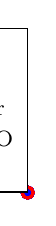
\begin{tikzpicture}[trim axis left, trim axis right]

\begin{axis}[%
width=\figurewidth,
height=\figureheight,
at={(0\figurewidth,0\figureheight)},
scale only axis,
unbounded coords=jump,
every outer x axis line/.append style={black},
every x tick label/.append style={font=\color{black}},
xmin=0,
xmax=300,
xtick={0, 100, 200, 300},
xlabel={Time},
every outer y axis line/.append style={black},
every y tick label/.append style={font=\color{black}},
ymin=33.57,
ymax=33.7,
yticklabel style={
        /pgf/number format/fixed,
        /pgf/number format/precision=2
},
ylabel={Price},
axis background/.style={fill=white},
legend style={legend cell align=left,align=left,draw=black,font=\footnotesize, at={(0.98,0.02)},anchor=south east}
]
\addplot [color=black,solid,line width=3.0pt,forget plot]
  table[row sep=crcr]{%
0.02	33.61\\
0.04	33.61\\
0.06	33.61\\
0.08	33.61\\
0.1	33.61\\
0.12	33.61\\
0.14	33.61\\
0.16	33.61\\
0.18	33.61\\
0.2	33.61\\
0.22	33.61\\
0.24	33.61\\
0.26	33.61\\
0.28	33.61\\
0.3	33.61\\
0.32	33.61\\
0.34	33.61\\
0.36	33.61\\
0.38	33.61\\
0.4	33.61\\
0.42	33.61\\
0.44	33.61\\
0.46	33.61\\
0.48	33.61\\
0.5	33.61\\
0.52	33.61\\
0.54	33.61\\
0.56	33.61\\
0.58	33.61\\
0.6	33.61\\
0.62	33.61\\
0.64	33.61\\
0.66	33.61\\
0.68	33.61\\
0.7	33.61\\
0.72	33.61\\
0.74	33.61\\
0.76	33.61\\
0.78	33.61\\
0.8	33.61\\
0.82	33.61\\
0.84	33.61\\
0.86	33.61\\
0.88	33.61\\
0.9	33.61\\
0.92	33.61\\
0.94	33.61\\
0.96	33.61\\
0.98	33.61\\
1	33.61\\
1.02	33.61\\
1.04	33.61\\
1.06	33.61\\
1.08	33.61\\
1.1	33.61\\
1.12	33.61\\
1.14	33.61\\
1.16	33.61\\
1.18	33.61\\
1.2	33.61\\
1.22	33.61\\
1.24	33.61\\
1.26	33.61\\
1.28	33.61\\
1.3	33.61\\
1.32	33.61\\
1.34	33.61\\
1.36	33.61\\
1.38	33.61\\
1.4	33.61\\
1.42	33.61\\
1.44	33.61\\
1.46	33.61\\
1.48	33.61\\
1.5	33.61\\
1.52	33.61\\
1.54	33.61\\
1.56	33.61\\
1.58	33.61\\
1.6	33.61\\
1.62	33.61\\
1.64	33.61\\
1.66	33.61\\
1.68	33.61\\
1.7	33.61\\
1.72	33.61\\
1.74	33.61\\
1.76	33.61\\
1.78	33.61\\
1.8	33.61\\
1.82	33.61\\
1.84	33.61\\
1.86	33.61\\
1.88	33.61\\
1.9	33.61\\
1.92	33.61\\
1.94	33.61\\
1.96	33.61\\
1.98	33.61\\
2	33.61\\
2.02	33.61\\
2.04	33.61\\
2.06	33.61\\
2.08	33.61\\
2.1	33.61\\
2.12	33.61\\
2.14	33.61\\
2.16	33.61\\
2.18	33.61\\
2.2	33.61\\
2.22	33.61\\
2.24	33.61\\
2.26	33.61\\
2.28	33.61\\
2.3	33.61\\
2.32	33.61\\
2.34	33.61\\
2.36	33.61\\
2.38	33.61\\
2.4	33.61\\
2.42	33.61\\
2.44	33.61\\
2.46	33.61\\
2.48	33.61\\
2.5	33.61\\
2.52	33.61\\
2.54	33.61\\
2.56	33.61\\
2.58	33.61\\
2.6	33.61\\
2.62	33.61\\
2.64	33.61\\
2.66	33.61\\
2.68	33.61\\
2.7	33.61\\
2.72	33.61\\
2.74	33.61\\
2.76	33.61\\
2.78	33.61\\
2.8	33.61\\
2.82	33.61\\
2.84	33.61\\
2.86	33.61\\
2.88	33.61\\
2.9	33.61\\
2.92	33.61\\
2.94	33.61\\
2.96	33.61\\
2.98	33.61\\
3	33.61\\
3.02	33.61\\
3.04	33.61\\
3.06	33.61\\
3.08	33.61\\
3.1	33.61\\
3.12	33.61\\
3.14	33.61\\
3.16	33.61\\
3.18	33.61\\
3.2	33.61\\
3.22	33.61\\
3.24	33.61\\
3.26	33.61\\
3.28	33.61\\
3.3	33.61\\
3.32	33.61\\
3.34	33.61\\
3.36	33.61\\
3.38	33.61\\
3.4	33.61\\
3.42	33.61\\
3.44	33.61\\
3.46	33.61\\
3.48	33.61\\
3.5	33.61\\
3.52	33.61\\
3.54	33.61\\
3.56	33.61\\
3.58	33.61\\
3.6	33.61\\
3.62	33.61\\
3.64	33.61\\
3.66	33.61\\
3.68	33.61\\
3.7	33.61\\
3.72	33.61\\
3.74	33.61\\
3.76	33.61\\
3.78	33.61\\
3.8	33.61\\
3.82	33.61\\
3.84	33.61\\
3.86	33.61\\
3.88	33.61\\
3.9	33.61\\
3.92	33.61\\
3.94	33.61\\
3.96	33.61\\
3.98	33.61\\
4	33.61\\
4.02	33.61\\
4.04	33.61\\
4.06	33.61\\
4.08	33.61\\
4.1	33.61\\
4.12	33.61\\
4.14	33.61\\
4.16	33.61\\
4.18	33.61\\
4.2	33.61\\
4.22	33.61\\
4.24	33.61\\
4.26	33.61\\
4.28	33.61\\
4.3	33.61\\
4.32	33.61\\
4.34	33.61\\
4.36	33.61\\
4.38	33.61\\
4.4	33.61\\
4.42	33.61\\
4.44	33.61\\
4.46	33.61\\
4.48	33.61\\
4.5	33.61\\
4.52	33.61\\
4.54	33.61\\
4.56	33.61\\
4.58	33.61\\
4.6	33.61\\
4.62	33.61\\
4.64	33.61\\
4.66	33.61\\
4.68	33.61\\
4.7	33.61\\
4.72	33.61\\
4.74	33.61\\
4.76	33.61\\
4.78	33.61\\
4.8	33.61\\
4.82	33.61\\
4.84	33.61\\
4.86	33.61\\
4.88	33.61\\
4.9	33.61\\
4.92	33.61\\
4.94	33.61\\
4.96	33.61\\
4.98	33.61\\
5	33.61\\
5.02	33.61\\
5.04	33.61\\
5.06	33.61\\
5.08	33.61\\
5.1	33.61\\
5.12	33.61\\
5.14	33.61\\
5.16	33.61\\
5.18	33.61\\
5.2	33.61\\
5.22	33.61\\
5.24	33.61\\
5.26	33.61\\
5.28	33.61\\
5.3	33.61\\
5.32	33.61\\
5.34	33.61\\
5.36	33.61\\
5.38	33.61\\
5.4	33.61\\
5.42	33.61\\
5.44	33.61\\
5.46	33.61\\
5.48	33.61\\
5.5	33.61\\
5.52	33.61\\
5.54	33.61\\
5.56	33.61\\
5.58	33.61\\
5.6	33.61\\
5.62	33.61\\
5.64	33.61\\
5.66	33.61\\
5.68	33.61\\
5.7	33.61\\
5.72	33.61\\
5.74	33.61\\
5.76	33.61\\
5.78	33.61\\
5.8	33.61\\
5.82	33.61\\
5.84	33.61\\
5.86	33.61\\
5.88	33.61\\
5.9	33.61\\
5.92	33.61\\
5.94	33.61\\
5.96	33.61\\
5.98	33.61\\
6	33.61\\
6.02	33.61\\
6.04	33.61\\
6.06	33.61\\
6.08	33.61\\
6.1	33.61\\
6.12	33.61\\
6.14	33.61\\
6.16	33.61\\
6.18	33.61\\
6.2	33.61\\
6.22	33.61\\
6.24	33.61\\
6.26	33.61\\
6.28	33.61\\
6.3	33.61\\
6.32	33.61\\
6.34	33.61\\
6.36	33.61\\
6.38	33.61\\
6.4	33.61\\
6.42	33.61\\
6.44	33.61\\
6.46	33.61\\
6.48	33.61\\
6.5	33.61\\
6.52	33.61\\
6.54	33.61\\
6.56	33.61\\
6.58	33.61\\
6.6	33.61\\
6.62	33.61\\
6.64	33.61\\
6.66	33.61\\
6.68	33.61\\
6.7	33.61\\
6.72	33.61\\
6.74	33.61\\
6.76	33.61\\
6.78	33.61\\
6.8	33.61\\
6.82	33.61\\
6.84	33.61\\
6.86	33.61\\
6.88	33.61\\
6.9	33.61\\
6.92	33.61\\
6.94	33.61\\
6.96	33.61\\
6.98	33.61\\
7	33.61\\
7.02	33.61\\
7.04	33.61\\
7.06	33.61\\
7.08	33.61\\
7.1	33.61\\
7.12	33.61\\
7.14	33.61\\
7.16	33.61\\
7.18	33.61\\
7.2	33.61\\
7.22	33.61\\
7.24	33.61\\
7.26	33.61\\
7.28	33.61\\
7.3	33.61\\
7.32	33.61\\
7.34	33.61\\
7.36	33.61\\
7.38	33.61\\
7.4	33.61\\
7.42	33.61\\
7.44	33.61\\
7.46	33.61\\
7.48	33.61\\
7.5	33.61\\
7.52	33.61\\
7.54	33.61\\
7.56	33.61\\
7.58	33.61\\
7.6	33.61\\
7.62	33.61\\
7.64	33.61\\
7.66	33.61\\
7.68	33.61\\
7.7	33.61\\
7.72	33.61\\
7.74	33.61\\
7.76	33.61\\
7.78	33.61\\
7.8	33.61\\
7.82	33.61\\
7.84	33.61\\
7.86	33.61\\
7.88	33.61\\
7.9	33.61\\
7.92	33.61\\
7.94	33.61\\
7.96	33.61\\
7.98	33.61\\
8	33.61\\
8.02	33.61\\
8.04	33.61\\
8.06	33.61\\
8.08	33.61\\
8.1	33.61\\
8.12	33.61\\
8.14	33.61\\
8.16	33.61\\
8.18	33.61\\
8.2	33.61\\
8.22	33.61\\
8.24	33.61\\
8.26	33.61\\
8.28	33.61\\
8.3	33.61\\
8.32	33.61\\
8.34	33.61\\
8.36	33.61\\
8.38	33.61\\
8.4	33.61\\
8.42	33.61\\
8.44	33.61\\
8.46	33.61\\
8.48	33.61\\
8.5	33.61\\
8.52	33.61\\
8.54	33.61\\
8.56	33.61\\
8.58	33.61\\
8.6	33.61\\
8.62	33.61\\
8.64	33.61\\
8.66	33.61\\
8.68	33.61\\
8.7	33.61\\
8.72	33.61\\
8.74	33.61\\
8.76	33.61\\
8.78	33.61\\
8.8	33.61\\
8.82	33.61\\
8.84	33.61\\
8.86	33.61\\
8.88	33.61\\
8.9	33.61\\
8.92	33.61\\
8.94	33.61\\
8.96	33.61\\
8.98	33.61\\
9	33.61\\
9.02	33.61\\
9.04	33.61\\
9.06	33.61\\
9.08	33.61\\
9.1	33.61\\
9.12	33.61\\
9.14	33.61\\
9.16	33.61\\
9.18	33.61\\
9.2	33.61\\
9.22	33.61\\
9.24	33.61\\
9.26	33.61\\
9.28	33.61\\
9.3	33.61\\
9.32	33.61\\
9.34	33.61\\
9.36	33.61\\
9.38	33.61\\
9.4	33.61\\
9.42	33.61\\
9.44	33.61\\
9.46	33.61\\
9.48	33.61\\
9.5	33.61\\
9.52	33.61\\
9.54	33.61\\
9.56	33.61\\
9.58	33.61\\
9.6	33.61\\
9.62	33.61\\
9.64	33.61\\
9.66	33.61\\
9.68	33.61\\
9.7	33.61\\
9.72	33.61\\
9.74	33.61\\
9.76	33.61\\
9.78	33.61\\
9.8	33.61\\
9.82	33.61\\
9.84	33.61\\
9.86	33.61\\
9.88	33.61\\
9.9	33.61\\
9.92	33.61\\
9.94	33.61\\
9.96	33.61\\
9.98	33.61\\
10	33.61\\
10.02	33.61\\
10.04	33.61\\
10.06	33.61\\
10.08	33.61\\
10.1	33.61\\
10.12	33.61\\
10.14	33.61\\
10.16	33.61\\
10.18	33.61\\
10.2	33.61\\
10.22	33.61\\
10.24	33.61\\
10.26	33.61\\
10.28	33.61\\
10.3	33.61\\
10.32	33.61\\
10.34	33.61\\
10.36	33.61\\
10.38	33.61\\
10.4	33.61\\
10.42	33.61\\
10.44	33.61\\
10.46	33.61\\
10.48	33.61\\
10.5	33.61\\
10.52	33.61\\
10.54	33.61\\
10.56	33.61\\
10.58	33.61\\
10.6	33.61\\
10.62	33.61\\
10.64	33.61\\
10.66	33.61\\
10.68	33.61\\
10.7	33.61\\
10.72	33.61\\
10.74	33.61\\
10.76	33.61\\
10.78	33.61\\
10.8	33.61\\
10.82	33.61\\
10.84	33.61\\
10.86	33.61\\
10.88	33.61\\
10.9	33.61\\
10.92	33.61\\
10.94	33.61\\
10.96	33.61\\
10.98	33.61\\
11	33.61\\
11.02	33.61\\
11.04	33.61\\
11.06	33.61\\
11.08	33.61\\
11.1	33.61\\
11.12	33.61\\
11.14	33.61\\
11.16	33.61\\
11.18	33.61\\
11.2	33.61\\
11.22	33.61\\
11.24	33.61\\
11.26	33.61\\
11.28	33.61\\
11.3	33.61\\
11.32	33.61\\
11.34	33.61\\
11.36	33.61\\
11.38	33.61\\
11.4	33.61\\
11.42	33.61\\
11.44	33.61\\
11.46	33.61\\
11.48	33.61\\
11.5	33.61\\
11.52	33.61\\
11.54	33.61\\
11.56	33.61\\
11.58	33.61\\
11.6	33.61\\
11.62	33.61\\
11.64	33.61\\
11.66	33.61\\
11.68	33.61\\
11.7	33.61\\
11.72	33.61\\
11.74	33.61\\
11.76	33.61\\
11.78	33.61\\
11.8	33.61\\
11.82	33.61\\
11.84	33.61\\
11.86	33.61\\
11.88	33.61\\
11.9	33.61\\
11.92	33.61\\
11.94	33.61\\
11.96	33.61\\
11.98	33.61\\
12	33.61\\
12.02	33.61\\
12.04	33.61\\
12.06	33.61\\
12.08	33.61\\
12.1	33.61\\
12.12	33.61\\
12.14	33.61\\
12.16	33.61\\
12.18	33.61\\
12.2	33.61\\
12.22	33.61\\
12.24	33.61\\
12.26	33.61\\
12.28	33.61\\
12.3	33.61\\
12.32	33.61\\
12.34	33.61\\
12.36	33.61\\
12.38	33.61\\
12.4	33.61\\
12.42	33.61\\
12.44	33.61\\
12.46	33.61\\
12.48	33.61\\
12.5	33.61\\
12.52	33.61\\
12.54	33.61\\
12.56	33.61\\
12.58	33.61\\
12.6	33.61\\
12.62	33.61\\
12.64	33.61\\
12.66	33.61\\
12.68	33.61\\
12.7	33.61\\
12.72	33.61\\
12.74	33.61\\
12.76	33.61\\
12.78	33.61\\
12.8	33.61\\
12.82	33.61\\
12.84	33.61\\
12.86	33.61\\
12.88	33.61\\
12.9	33.61\\
12.92	33.61\\
12.94	33.61\\
12.96	33.61\\
12.98	33.61\\
13	33.61\\
13.02	33.61\\
13.04	33.61\\
13.06	33.61\\
13.08	33.61\\
13.1	33.61\\
13.12	33.61\\
13.14	33.61\\
13.16	33.61\\
13.18	33.61\\
13.2	33.61\\
13.22	33.61\\
13.24	33.61\\
13.26	33.61\\
13.28	33.61\\
13.3	33.61\\
13.32	33.61\\
13.34	33.61\\
13.36	33.61\\
13.38	33.61\\
13.4	33.61\\
13.42	33.61\\
13.44	33.61\\
13.46	33.61\\
13.48	33.61\\
13.5	33.61\\
13.52	33.61\\
13.54	33.61\\
13.56	33.61\\
13.58	33.61\\
13.6	33.61\\
13.62	33.61\\
13.64	33.61\\
13.66	33.61\\
13.68	33.61\\
13.7	33.61\\
13.72	33.61\\
13.74	33.61\\
13.76	33.61\\
13.78	33.61\\
13.8	33.61\\
13.82	33.61\\
13.84	33.61\\
13.86	33.61\\
13.88	33.61\\
13.9	33.61\\
13.92	33.61\\
13.94	33.61\\
13.96	33.61\\
13.98	33.61\\
14	33.61\\
14.02	33.61\\
14.04	33.61\\
14.06	33.61\\
14.08	33.61\\
14.1	33.61\\
14.12	33.61\\
14.14	33.61\\
14.16	33.61\\
14.18	33.61\\
14.2	33.61\\
14.22	33.61\\
14.24	33.61\\
14.26	33.61\\
14.28	33.61\\
14.3	33.61\\
14.32	33.61\\
14.34	33.61\\
14.36	33.61\\
14.38	33.61\\
14.4	33.61\\
14.42	33.61\\
14.44	33.61\\
14.46	33.61\\
14.48	33.61\\
14.5	33.61\\
14.52	33.61\\
14.54	33.61\\
14.56	33.61\\
14.58	33.61\\
14.6	33.61\\
14.62	33.61\\
14.64	33.61\\
14.66	33.61\\
14.68	33.61\\
14.7	33.61\\
14.72	33.61\\
14.74	33.61\\
14.76	33.61\\
14.78	33.61\\
14.8	33.61\\
14.82	33.61\\
14.84	33.61\\
14.86	33.61\\
14.88	33.61\\
14.9	33.61\\
14.92	33.61\\
14.94	33.61\\
14.96	33.61\\
14.98	33.61\\
15	33.61\\
15.02	33.61\\
15.04	33.61\\
15.06	33.61\\
15.08	33.61\\
15.1	33.61\\
15.12	33.61\\
15.14	33.61\\
15.16	33.61\\
15.18	33.61\\
15.2	33.61\\
15.22	33.61\\
15.24	33.61\\
15.26	33.61\\
15.28	33.61\\
15.3	33.61\\
15.32	33.61\\
15.34	33.61\\
15.36	33.61\\
15.38	33.61\\
15.4	33.61\\
15.42	33.61\\
15.44	33.61\\
15.46	33.61\\
15.48	33.61\\
15.5	33.61\\
15.52	33.61\\
15.54	33.61\\
15.56	33.61\\
15.58	33.61\\
15.6	33.61\\
15.62	33.61\\
15.64	33.61\\
15.66	33.61\\
15.68	33.61\\
15.7	33.61\\
15.72	33.61\\
15.74	33.61\\
15.76	33.61\\
15.78	33.61\\
15.8	33.61\\
15.82	33.61\\
15.84	33.61\\
15.86	33.61\\
15.88	33.61\\
15.9	33.61\\
15.92	33.61\\
15.94	33.61\\
15.96	33.61\\
15.98	33.61\\
16	33.61\\
16.02	33.61\\
16.04	33.61\\
16.06	33.61\\
16.08	33.61\\
16.1	33.61\\
16.12	33.61\\
16.14	33.61\\
16.16	33.61\\
16.18	33.61\\
16.2	33.61\\
16.22	33.61\\
16.24	33.61\\
16.26	33.61\\
16.28	33.61\\
16.3	33.61\\
16.32	33.61\\
16.34	33.61\\
16.36	33.61\\
16.38	33.61\\
16.4	33.61\\
16.42	33.61\\
16.44	33.61\\
16.46	33.61\\
16.48	33.61\\
16.5	33.61\\
16.52	33.61\\
16.54	33.61\\
16.56	33.61\\
16.58	33.61\\
16.6	33.61\\
16.62	33.61\\
16.64	33.61\\
16.66	33.61\\
16.68	33.61\\
16.7	33.61\\
16.72	33.61\\
16.74	33.61\\
16.76	33.61\\
16.78	33.61\\
16.8	33.61\\
16.82	33.61\\
16.84	33.61\\
16.86	33.61\\
16.88	33.61\\
16.9	33.61\\
16.92	33.61\\
16.94	33.61\\
16.96	33.61\\
16.98	33.61\\
17	33.61\\
17.02	33.61\\
17.04	33.61\\
17.06	33.61\\
17.08	33.61\\
17.1	33.61\\
17.12	33.61\\
17.14	33.61\\
17.16	33.61\\
17.18	33.61\\
17.2	33.61\\
17.22	33.61\\
17.24	33.61\\
17.26	33.61\\
17.28	33.61\\
17.3	33.61\\
17.32	33.61\\
17.34	33.61\\
17.36	33.61\\
17.38	33.61\\
17.4	33.61\\
17.42	33.61\\
17.44	33.61\\
17.46	33.61\\
17.48	33.61\\
17.5	33.61\\
17.52	33.61\\
17.54	33.61\\
17.56	33.61\\
17.58	33.61\\
17.6	33.61\\
17.62	33.61\\
17.64	33.61\\
17.66	33.61\\
17.68	33.61\\
17.7	33.61\\
17.72	33.61\\
17.74	33.61\\
17.76	33.61\\
17.78	33.61\\
17.8	33.61\\
17.82	33.61\\
17.84	33.61\\
17.86	33.61\\
17.88	33.61\\
17.9	33.61\\
17.92	33.61\\
17.94	33.61\\
17.96	33.61\\
17.98	33.61\\
18	33.61\\
18.02	33.61\\
18.04	33.61\\
18.06	33.61\\
18.08	33.61\\
18.1	33.61\\
18.12	33.61\\
18.14	33.61\\
18.16	33.61\\
18.18	33.61\\
18.2	33.61\\
18.22	33.61\\
18.24	33.61\\
18.26	33.61\\
18.28	33.61\\
18.3	33.61\\
18.32	33.61\\
18.34	33.61\\
18.36	33.61\\
18.38	33.61\\
18.4	33.61\\
18.42	33.61\\
18.44	33.61\\
18.46	33.61\\
18.48	33.61\\
18.5	33.61\\
18.52	33.61\\
18.54	33.61\\
18.56	33.61\\
18.58	33.61\\
18.6	33.61\\
18.62	33.61\\
18.64	33.61\\
18.66	33.61\\
18.68	33.61\\
18.7	33.61\\
18.72	33.61\\
18.74	33.61\\
18.76	33.61\\
18.78	33.61\\
18.8	33.61\\
18.82	33.61\\
18.84	33.61\\
18.86	33.61\\
18.88	33.61\\
18.9	33.61\\
18.92	33.61\\
18.94	33.61\\
18.96	33.61\\
18.98	33.61\\
19	33.61\\
19.02	33.61\\
19.04	33.61\\
19.06	33.61\\
19.08	33.61\\
19.1	33.61\\
19.12	33.61\\
19.14	33.61\\
19.16	33.61\\
19.18	33.61\\
19.2	33.61\\
19.22	33.61\\
19.24	33.61\\
19.26	33.61\\
19.28	33.61\\
19.3	33.61\\
19.32	33.61\\
19.34	33.61\\
19.36	33.61\\
19.38	33.61\\
19.4	33.61\\
19.42	33.61\\
19.44	33.61\\
19.46	33.61\\
19.48	33.61\\
19.5	33.61\\
19.52	33.61\\
19.54	33.61\\
19.56	33.61\\
19.58	33.61\\
19.6	33.61\\
19.62	33.61\\
19.64	33.61\\
19.66	33.61\\
19.68	33.61\\
19.7	33.61\\
19.72	33.61\\
19.74	33.61\\
19.76	33.61\\
19.78	33.61\\
19.8	33.61\\
19.82	33.61\\
19.84	33.61\\
19.86	33.61\\
19.88	33.61\\
19.9	33.61\\
19.92	33.61\\
19.94	33.61\\
19.96	33.61\\
19.98	33.61\\
20	33.61\\
20.02	33.61\\
20.04	33.61\\
20.06	33.61\\
20.08	33.61\\
20.1	33.61\\
20.12	33.61\\
20.14	33.61\\
20.16	33.61\\
20.18	33.61\\
20.2	33.61\\
20.22	33.61\\
20.24	33.61\\
20.26	33.61\\
20.28	33.61\\
20.3	33.61\\
20.32	33.61\\
20.34	33.61\\
20.36	33.61\\
20.38	33.61\\
20.4	33.61\\
20.42	33.61\\
20.44	33.61\\
20.46	33.61\\
20.48	33.61\\
20.5	33.61\\
20.52	33.61\\
20.54	33.61\\
20.56	33.61\\
20.58	33.61\\
20.6	33.61\\
20.62	33.61\\
20.64	33.61\\
20.66	33.61\\
20.68	33.61\\
20.7	33.61\\
20.72	33.61\\
20.74	33.61\\
20.76	33.61\\
20.78	33.61\\
20.8	33.61\\
20.82	33.61\\
20.84	33.61\\
20.86	33.61\\
20.88	33.61\\
20.9	33.61\\
20.92	33.61\\
20.94	33.61\\
20.96	33.61\\
20.98	33.61\\
21	33.61\\
21.02	33.61\\
21.04	33.61\\
21.06	33.61\\
21.08	33.61\\
21.1	33.61\\
21.12	33.61\\
21.14	33.61\\
21.16	33.61\\
21.18	33.61\\
21.2	33.61\\
21.22	33.61\\
21.24	33.61\\
21.26	33.61\\
21.28	33.61\\
21.3	33.61\\
21.32	33.61\\
21.34	33.61\\
21.36	33.61\\
21.38	33.61\\
21.4	33.61\\
21.42	33.61\\
21.44	33.61\\
21.46	33.61\\
21.48	33.61\\
21.5	33.61\\
21.52	33.61\\
21.54	33.61\\
21.56	33.61\\
21.58	33.61\\
21.6	33.61\\
21.62	33.61\\
21.64	33.61\\
21.66	33.61\\
21.68	33.61\\
21.7	33.61\\
21.72	33.61\\
21.74	33.61\\
21.76	33.61\\
21.78	33.61\\
21.8	33.61\\
21.82	33.61\\
21.84	33.61\\
21.86	33.61\\
21.88	33.61\\
21.9	33.61\\
21.92	33.61\\
21.94	33.61\\
21.96	33.61\\
21.98	33.61\\
22	33.61\\
22.02	33.61\\
22.04	33.61\\
22.06	33.61\\
22.08	33.61\\
22.1	33.61\\
22.12	33.61\\
22.14	33.61\\
22.16	33.61\\
22.18	33.61\\
22.2	33.61\\
22.22	33.61\\
22.24	33.61\\
22.26	33.61\\
22.28	33.61\\
22.3	33.61\\
22.32	33.61\\
22.34	33.61\\
22.36	33.61\\
22.38	33.61\\
22.4	33.61\\
22.42	33.61\\
22.44	33.61\\
22.46	33.61\\
22.48	33.61\\
22.5	33.61\\
22.52	33.61\\
22.54	33.61\\
22.56	33.61\\
22.58	33.61\\
22.6	33.61\\
22.62	33.61\\
22.64	33.61\\
22.66	33.61\\
22.68	33.61\\
22.7	33.61\\
22.72	33.61\\
22.74	33.61\\
22.76	33.61\\
22.78	33.61\\
22.8	33.61\\
22.82	33.61\\
22.84	33.61\\
22.86	33.61\\
22.88	33.61\\
22.9	33.61\\
22.92	33.61\\
22.94	33.61\\
22.96	33.61\\
22.98	33.61\\
23	33.61\\
23.02	33.61\\
23.04	33.61\\
23.06	33.61\\
23.08	33.61\\
23.1	33.61\\
23.12	33.61\\
23.14	33.61\\
23.16	33.61\\
23.18	33.61\\
23.2	33.61\\
23.22	33.61\\
23.24	33.61\\
23.26	33.61\\
23.28	33.61\\
23.3	33.61\\
23.32	33.61\\
23.34	33.61\\
23.36	33.61\\
23.38	33.61\\
23.4	33.61\\
23.42	33.61\\
23.44	33.61\\
23.46	33.61\\
23.48	33.61\\
23.5	33.61\\
23.52	33.61\\
23.54	33.61\\
23.56	33.61\\
23.58	33.61\\
23.6	33.61\\
23.62	33.61\\
23.64	33.61\\
23.66	33.61\\
23.68	33.61\\
23.7	33.61\\
23.72	33.61\\
23.74	33.61\\
23.76	33.61\\
23.78	33.61\\
23.8	33.61\\
23.82	33.61\\
23.84	33.61\\
23.86	33.61\\
23.88	33.61\\
23.9	33.61\\
23.92	33.61\\
23.94	33.61\\
23.96	33.61\\
23.98	33.61\\
24	33.61\\
24.02	33.61\\
24.04	33.61\\
24.06	33.61\\
24.08	33.61\\
24.1	33.61\\
24.12	33.61\\
24.14	33.61\\
24.16	33.61\\
24.18	33.61\\
24.2	33.61\\
24.22	33.61\\
24.24	33.61\\
24.26	33.61\\
24.28	33.61\\
24.3	33.61\\
24.32	33.61\\
24.34	33.61\\
24.36	33.61\\
24.38	33.61\\
24.4	33.61\\
24.42	33.61\\
24.44	33.61\\
24.46	33.61\\
24.48	33.61\\
24.5	33.61\\
24.52	33.61\\
24.54	33.61\\
24.56	33.61\\
24.58	33.61\\
24.6	33.61\\
24.62	33.61\\
24.64	33.61\\
24.66	33.61\\
24.68	33.61\\
24.7	33.61\\
24.72	33.61\\
24.74	33.61\\
24.76	33.61\\
24.78	33.61\\
24.8	33.61\\
24.82	33.61\\
24.84	33.61\\
24.86	33.61\\
24.88	33.61\\
24.9	33.61\\
24.92	33.61\\
24.94	33.61\\
24.96	33.61\\
24.98	33.61\\
25	33.61\\
25.02	33.61\\
25.04	33.61\\
25.06	33.61\\
25.08	33.61\\
25.1	33.61\\
25.12	33.61\\
25.14	33.61\\
25.16	33.61\\
25.18	33.61\\
25.2	33.61\\
25.22	33.61\\
25.24	33.61\\
25.26	33.61\\
25.28	33.61\\
25.3	33.61\\
25.32	33.61\\
25.34	33.61\\
25.36	33.61\\
25.38	33.61\\
25.4	33.61\\
25.42	33.61\\
25.44	33.61\\
25.46	33.61\\
25.48	33.61\\
25.5	33.61\\
25.52	33.61\\
25.54	33.61\\
25.56	33.61\\
25.58	33.61\\
25.6	33.61\\
25.62	33.61\\
25.64	33.61\\
25.66	33.61\\
25.68	33.61\\
25.7	33.61\\
25.72	33.61\\
25.74	33.61\\
25.76	33.61\\
25.78	33.61\\
25.8	33.61\\
25.82	33.61\\
25.84	33.61\\
25.86	33.61\\
25.88	33.61\\
25.9	33.61\\
25.92	33.61\\
25.94	33.61\\
25.96	33.61\\
25.98	33.61\\
26	33.61\\
26.02	33.61\\
26.04	33.61\\
26.06	33.61\\
26.08	33.61\\
26.1	33.61\\
26.12	33.61\\
26.14	33.61\\
26.16	33.61\\
26.18	33.61\\
26.2	33.61\\
26.22	33.61\\
26.24	33.61\\
26.26	33.61\\
26.28	33.61\\
26.3	33.61\\
26.32	33.61\\
26.34	33.61\\
26.36	33.61\\
26.38	33.61\\
26.4	33.61\\
26.42	33.61\\
26.44	33.61\\
26.46	33.61\\
26.48	33.61\\
26.5	33.61\\
26.52	33.61\\
26.54	33.61\\
26.56	33.61\\
26.58	33.61\\
26.6	33.61\\
26.62	33.61\\
26.64	33.61\\
26.66	33.61\\
26.68	33.61\\
26.7	33.61\\
26.72	33.61\\
26.74	33.61\\
26.76	33.61\\
26.78	33.61\\
26.8	33.61\\
26.82	33.61\\
26.84	33.61\\
26.86	33.61\\
26.88	33.61\\
26.9	33.61\\
26.92	33.61\\
26.94	33.61\\
26.96	33.61\\
26.98	33.61\\
27	33.61\\
27.02	33.61\\
27.04	33.61\\
27.06	33.61\\
27.08	33.61\\
27.1	33.61\\
27.12	33.61\\
27.14	33.61\\
27.16	33.61\\
27.18	33.61\\
27.2	33.61\\
27.22	33.61\\
27.24	33.61\\
27.26	33.61\\
27.28	33.61\\
27.3	33.61\\
27.32	33.61\\
27.34	33.61\\
27.36	33.61\\
27.38	33.61\\
27.4	33.61\\
27.42	33.61\\
27.44	33.61\\
27.46	33.61\\
27.48	33.61\\
27.5	33.61\\
27.52	33.61\\
27.54	33.61\\
27.56	33.61\\
27.58	33.61\\
27.6	33.61\\
27.62	33.61\\
27.64	33.61\\
27.66	33.61\\
27.68	33.61\\
27.7	33.61\\
27.72	33.61\\
27.74	33.61\\
27.76	33.61\\
27.78	33.61\\
27.8	33.61\\
27.82	33.61\\
27.84	33.61\\
27.86	33.61\\
27.88	33.61\\
27.9	33.61\\
27.92	33.61\\
27.94	33.61\\
27.96	33.61\\
27.98	33.61\\
28	33.61\\
28.02	33.61\\
28.04	33.61\\
28.06	33.61\\
28.08	33.61\\
28.1	33.61\\
28.12	33.61\\
28.14	33.61\\
28.16	33.61\\
28.18	33.61\\
28.2	33.61\\
28.22	33.61\\
28.24	33.61\\
28.26	33.61\\
28.28	33.61\\
28.3	33.61\\
28.32	33.61\\
28.34	33.61\\
28.36	33.61\\
28.38	33.61\\
28.4	33.61\\
28.42	33.61\\
28.44	33.61\\
28.46	33.61\\
28.48	33.61\\
28.5	33.61\\
28.52	33.61\\
28.54	33.61\\
28.56	33.61\\
28.58	33.61\\
28.6	33.61\\
28.62	33.61\\
28.64	33.61\\
28.66	33.61\\
28.68	33.61\\
28.7	33.61\\
28.72	33.61\\
28.74	33.61\\
28.76	33.61\\
28.78	33.61\\
28.8	33.61\\
28.82	33.61\\
28.84	33.61\\
28.86	33.61\\
28.88	33.61\\
28.9	33.61\\
28.92	33.61\\
28.94	33.61\\
28.96	33.61\\
28.98	33.61\\
29	33.61\\
29.02	33.61\\
29.04	33.61\\
29.06	33.61\\
29.08	33.61\\
29.1	33.61\\
29.12	33.61\\
29.14	33.61\\
29.16	33.61\\
29.18	33.61\\
29.2	33.61\\
29.22	33.61\\
29.24	33.61\\
29.26	33.61\\
29.28	33.61\\
29.3	33.61\\
29.32	33.61\\
29.34	33.61\\
29.36	33.61\\
29.38	33.61\\
29.4	33.61\\
29.42	33.61\\
29.44	33.61\\
29.46	33.61\\
29.48	33.61\\
29.5	33.61\\
29.52	33.61\\
29.54	33.61\\
29.56	33.61\\
29.58	33.61\\
29.6	33.61\\
29.62	33.61\\
29.64	33.61\\
29.66	33.61\\
29.68	33.61\\
29.7	33.61\\
29.72	33.61\\
29.74	33.61\\
29.76	33.61\\
29.78	33.61\\
29.8	33.61\\
29.82	33.61\\
29.84	33.61\\
29.86	33.61\\
29.88	33.61\\
29.9	33.61\\
29.92	33.61\\
29.94	33.61\\
29.96	33.61\\
29.98	33.61\\
30	33.61\\
30.02	33.61\\
30.04	33.61\\
30.06	33.61\\
30.08	33.61\\
30.1	33.61\\
30.12	33.61\\
30.14	33.61\\
30.16	33.61\\
30.18	33.61\\
30.2	33.61\\
30.22	33.61\\
30.24	33.61\\
30.26	33.61\\
30.28	33.61\\
30.3	33.61\\
30.32	33.61\\
30.34	33.61\\
30.36	33.61\\
30.38	33.61\\
30.4	33.61\\
30.42	33.61\\
30.44	33.61\\
30.46	33.61\\
30.48	33.61\\
30.5	33.61\\
30.52	33.61\\
30.54	33.61\\
30.56	33.61\\
30.58	33.61\\
30.6	33.61\\
30.62	33.61\\
30.64	33.61\\
30.66	33.61\\
30.68	33.61\\
30.7	33.61\\
30.72	33.61\\
30.74	33.61\\
30.76	33.61\\
30.78	33.61\\
30.8	33.61\\
30.82	33.61\\
30.84	33.61\\
30.86	33.61\\
30.88	33.61\\
30.9	33.61\\
30.92	33.61\\
30.94	33.61\\
30.96	33.61\\
30.98	33.61\\
31	33.61\\
31.02	33.61\\
31.04	33.61\\
31.06	33.61\\
31.08	33.61\\
31.1	33.61\\
31.12	33.61\\
31.14	33.61\\
31.16	33.61\\
31.18	33.61\\
31.2	33.61\\
31.22	33.61\\
31.24	33.61\\
31.26	33.61\\
31.28	33.61\\
31.3	33.61\\
31.32	33.61\\
31.34	33.61\\
31.36	33.61\\
31.38	33.61\\
31.4	33.61\\
31.42	33.61\\
31.44	33.61\\
31.46	33.61\\
31.48	33.61\\
31.5	33.61\\
31.52	33.61\\
31.54	33.61\\
31.56	33.61\\
31.58	33.61\\
31.6	33.61\\
31.62	33.61\\
31.64	33.61\\
31.66	33.61\\
31.68	33.61\\
31.7	33.61\\
31.72	33.61\\
31.74	33.61\\
31.76	33.61\\
31.78	33.61\\
31.8	33.61\\
31.82	33.61\\
31.84	33.61\\
31.86	33.61\\
31.88	33.61\\
31.9	33.61\\
31.92	33.61\\
31.94	33.61\\
31.96	33.61\\
31.98	33.61\\
32	33.61\\
32.02	33.61\\
32.04	33.61\\
32.06	33.61\\
32.08	33.61\\
32.1	33.61\\
32.12	33.61\\
32.14	33.61\\
32.16	33.61\\
32.18	33.61\\
32.2	33.61\\
32.22	33.61\\
32.24	33.61\\
32.26	33.61\\
32.28	33.61\\
32.3	33.61\\
32.32	33.61\\
32.34	33.61\\
32.36	33.61\\
32.38	33.61\\
32.4	33.61\\
32.42	33.61\\
32.44	33.61\\
32.46	33.61\\
32.48	33.61\\
32.5	33.61\\
32.52	33.61\\
32.54	33.61\\
32.56	33.61\\
32.58	33.61\\
32.6	33.61\\
32.62	33.61\\
32.64	33.61\\
32.66	33.61\\
32.68	33.61\\
32.7	33.61\\
32.72	33.61\\
32.74	33.61\\
32.76	33.61\\
32.78	33.61\\
32.8	33.61\\
32.82	33.61\\
32.84	33.61\\
32.86	33.61\\
32.88	33.61\\
32.9	33.61\\
32.92	33.61\\
32.94	33.61\\
32.96	33.61\\
32.98	33.61\\
33	33.61\\
33.02	33.61\\
33.04	33.61\\
33.06	33.61\\
33.08	33.61\\
33.1	33.61\\
33.12	33.61\\
33.14	33.61\\
33.16	33.61\\
33.18	33.61\\
33.2	33.61\\
33.22	33.61\\
33.24	33.61\\
33.26	33.61\\
33.28	33.61\\
33.3	33.61\\
33.32	33.61\\
33.34	33.61\\
33.36	33.61\\
33.38	33.61\\
33.4	33.61\\
33.42	33.61\\
33.44	33.61\\
33.46	33.61\\
33.48	33.61\\
33.5	33.61\\
33.52	33.61\\
33.54	33.61\\
33.56	33.61\\
33.58	33.61\\
33.6	33.61\\
33.62	33.61\\
33.64	33.61\\
33.66	33.61\\
33.68	33.61\\
33.7	33.61\\
33.72	33.61\\
33.74	33.61\\
33.76	33.61\\
33.78	33.61\\
33.8	33.61\\
33.82	33.61\\
33.84	33.61\\
33.86	33.61\\
33.88	33.61\\
33.9	33.61\\
33.92	33.61\\
33.94	33.61\\
33.96	33.61\\
33.98	33.61\\
34	33.61\\
34.02	33.61\\
34.04	33.61\\
34.06	33.61\\
34.08	33.61\\
34.1	33.61\\
34.12	33.61\\
34.14	33.61\\
34.16	33.61\\
34.18	33.61\\
34.2	33.61\\
34.22	33.61\\
34.24	33.61\\
34.26	33.61\\
34.28	33.61\\
34.3	33.61\\
34.32	33.61\\
34.34	33.61\\
34.36	33.61\\
34.38	33.61\\
34.4	33.61\\
34.42	33.61\\
34.44	33.61\\
34.46	33.61\\
34.48	33.61\\
34.5	33.61\\
34.52	33.61\\
34.54	33.61\\
34.56	33.61\\
34.58	33.61\\
34.6	33.61\\
34.62	33.61\\
34.64	33.61\\
34.66	33.61\\
34.68	33.61\\
34.7	33.61\\
34.72	33.61\\
34.74	33.61\\
34.76	33.61\\
34.78	33.61\\
34.8	33.61\\
34.82	33.61\\
34.84	33.61\\
34.86	33.61\\
34.88	33.61\\
34.9	33.61\\
34.92	33.61\\
34.94	33.61\\
34.96	33.61\\
34.98	33.61\\
35	33.61\\
35.02	33.61\\
35.04	33.61\\
35.06	33.61\\
35.08	33.61\\
35.1	33.61\\
35.12	33.61\\
35.14	33.61\\
35.16	33.61\\
35.18	33.61\\
35.2	33.61\\
35.22	33.61\\
35.24	33.61\\
35.26	33.61\\
35.28	33.61\\
35.3	33.61\\
35.32	33.61\\
35.34	33.61\\
35.36	33.61\\
35.38	33.61\\
35.4	33.61\\
35.42	33.61\\
35.44	33.61\\
35.46	33.61\\
35.48	33.61\\
35.5	33.61\\
35.52	33.61\\
35.54	33.61\\
35.56	33.61\\
35.58	33.61\\
35.6	33.61\\
35.62	33.61\\
35.64	33.61\\
35.66	33.61\\
35.68	33.61\\
35.7	33.61\\
35.72	33.61\\
35.74	33.61\\
35.76	33.61\\
35.78	33.61\\
35.8	33.61\\
35.82	33.61\\
35.84	33.61\\
35.86	33.61\\
35.88	33.61\\
35.9	33.61\\
35.92	33.61\\
35.94	33.61\\
35.96	33.61\\
35.98	33.61\\
36	33.61\\
36.02	33.61\\
36.04	33.61\\
36.06	33.61\\
36.08	33.61\\
36.1	33.61\\
36.12	33.61\\
36.14	33.61\\
36.16	33.61\\
36.18	33.61\\
36.2	33.61\\
36.22	33.61\\
36.24	33.61\\
36.26	33.61\\
36.28	33.61\\
36.3	33.61\\
36.32	33.61\\
36.34	33.61\\
36.36	33.61\\
36.38	33.61\\
36.4	33.61\\
36.42	33.61\\
36.44	33.61\\
36.46	33.61\\
36.48	33.61\\
36.5	33.61\\
36.52	33.61\\
36.54	33.61\\
36.56	33.61\\
36.58	33.61\\
36.6	33.61\\
36.62	33.61\\
36.64	33.61\\
36.66	33.61\\
36.68	33.61\\
36.7	33.61\\
36.72	33.61\\
36.74	33.61\\
36.76	33.61\\
36.78	33.61\\
36.8	33.61\\
36.82	33.61\\
36.84	33.61\\
36.86	33.61\\
36.88	33.61\\
36.9	33.61\\
36.92	33.61\\
36.94	33.61\\
36.96	33.61\\
36.98	33.61\\
37	33.61\\
37.02	33.61\\
37.04	33.61\\
37.06	33.61\\
37.08	33.61\\
37.1	33.61\\
37.12	33.61\\
37.14	33.61\\
37.16	33.61\\
37.18	33.61\\
37.2	33.61\\
37.22	33.61\\
37.24	33.61\\
37.26	33.61\\
37.28	33.61\\
37.3	33.61\\
37.32	33.61\\
37.34	33.61\\
37.36	33.61\\
37.38	33.61\\
37.4	33.61\\
37.42	33.61\\
37.44	33.61\\
37.46	33.61\\
37.48	33.61\\
37.5	33.61\\
37.52	33.61\\
37.54	33.61\\
37.56	33.61\\
37.58	33.61\\
37.6	33.61\\
37.62	33.61\\
37.64	33.61\\
37.66	33.61\\
37.68	33.61\\
37.7	33.61\\
37.72	33.61\\
37.74	33.61\\
37.76	33.61\\
37.78	33.61\\
37.8	33.61\\
37.82	33.61\\
37.84	33.61\\
37.86	33.61\\
37.88	33.61\\
37.9	33.61\\
37.92	33.61\\
37.94	33.61\\
37.96	33.61\\
37.98	33.61\\
38	33.61\\
38.02	33.61\\
38.04	33.61\\
38.06	33.61\\
38.08	33.61\\
38.1	33.61\\
38.12	33.61\\
38.14	33.61\\
38.16	33.61\\
38.18	33.61\\
38.2	33.61\\
38.22	33.61\\
38.24	33.61\\
38.26	33.61\\
38.28	33.61\\
38.3	33.61\\
38.32	33.61\\
38.34	33.61\\
38.36	33.61\\
38.38	33.61\\
38.4	33.61\\
38.42	33.61\\
38.44	33.61\\
38.46	33.61\\
38.48	33.61\\
38.5	33.61\\
38.52	33.61\\
38.54	33.61\\
38.56	33.61\\
38.58	33.61\\
38.6	33.61\\
38.62	33.61\\
38.64	33.61\\
38.66	33.61\\
38.68	33.61\\
38.7	33.61\\
38.72	33.61\\
38.74	33.61\\
38.76	33.61\\
38.78	33.61\\
38.8	33.61\\
38.82	33.61\\
38.84	33.61\\
38.86	33.61\\
38.88	33.61\\
38.9	33.61\\
38.92	33.61\\
38.94	33.61\\
38.96	33.61\\
38.98	33.61\\
39	33.61\\
39.02	33.61\\
39.04	33.61\\
39.06	33.61\\
39.08	33.61\\
39.1	33.61\\
39.12	33.61\\
39.14	33.61\\
39.16	33.61\\
39.18	33.61\\
39.2	33.61\\
39.22	33.61\\
39.24	33.61\\
39.26	33.61\\
39.28	33.61\\
39.3	33.61\\
39.32	33.61\\
39.34	33.61\\
39.36	33.61\\
39.38	33.61\\
39.4	33.61\\
39.42	33.61\\
39.44	33.61\\
39.46	33.61\\
39.48	33.61\\
39.5	33.61\\
39.52	33.61\\
39.54	33.61\\
39.56	33.61\\
39.58	33.61\\
39.6	33.61\\
39.62	33.61\\
39.64	33.61\\
39.66	33.61\\
39.68	33.61\\
39.7	33.61\\
39.72	33.61\\
39.74	33.61\\
39.76	33.61\\
39.78	33.61\\
39.8	33.61\\
39.82	33.61\\
39.84	33.61\\
39.86	33.61\\
39.88	33.61\\
39.9	33.61\\
39.92	33.61\\
39.94	33.61\\
39.96	33.61\\
39.98	33.61\\
40	33.61\\
40.02	33.61\\
40.04	33.61\\
40.06	33.61\\
40.08	33.61\\
40.1	33.61\\
40.12	33.61\\
40.14	33.61\\
40.16	33.61\\
40.18	33.61\\
40.2	33.61\\
40.22	33.61\\
40.24	33.61\\
40.26	33.61\\
40.28	33.61\\
40.3	33.61\\
40.32	33.61\\
40.34	33.61\\
40.36	33.61\\
40.38	33.61\\
40.4	33.61\\
40.42	33.61\\
40.44	33.61\\
40.46	33.61\\
40.48	33.61\\
40.5	33.61\\
40.52	33.61\\
40.54	33.61\\
40.56	33.61\\
40.58	33.61\\
40.6	33.61\\
40.62	33.61\\
40.64	33.61\\
40.66	33.61\\
40.68	33.61\\
40.7	33.61\\
40.72	33.61\\
40.74	33.61\\
40.76	33.61\\
40.78	33.61\\
40.8	33.61\\
40.82	33.61\\
40.84	33.61\\
40.86	33.61\\
40.88	33.61\\
40.9	33.61\\
40.92	33.61\\
40.94	33.61\\
40.96	33.61\\
40.98	33.61\\
41	33.61\\
41.02	33.61\\
41.04	33.61\\
41.06	33.61\\
41.08	33.61\\
41.1	33.61\\
41.12	33.61\\
41.14	33.61\\
41.16	33.61\\
41.18	33.61\\
41.2	33.61\\
41.22	33.61\\
41.24	33.61\\
41.26	33.61\\
41.28	33.61\\
41.3	33.61\\
41.32	33.61\\
41.34	33.61\\
41.36	33.61\\
41.38	33.61\\
41.4	33.61\\
41.42	33.61\\
41.44	33.61\\
41.46	33.61\\
41.48	33.61\\
41.5	33.61\\
41.52	33.61\\
41.54	33.61\\
41.56	33.61\\
41.58	33.61\\
41.6	33.61\\
41.62	33.61\\
41.64	33.61\\
41.66	33.61\\
41.68	33.61\\
41.7	33.61\\
41.72	33.61\\
41.74	33.61\\
41.76	33.61\\
41.78	33.61\\
41.8	33.61\\
41.82	33.61\\
41.84	33.61\\
41.86	33.61\\
41.88	33.61\\
41.9	33.61\\
41.92	33.61\\
41.94	33.61\\
41.96	33.61\\
41.98	33.61\\
42	33.61\\
42.02	33.61\\
42.04	33.61\\
42.06	33.61\\
42.08	33.61\\
42.1	33.61\\
42.12	33.61\\
42.14	33.61\\
42.16	33.61\\
42.18	33.61\\
42.2	33.61\\
42.22	33.61\\
42.24	33.61\\
42.26	33.61\\
42.28	33.61\\
42.3	33.61\\
42.32	33.61\\
42.34	33.61\\
42.36	33.61\\
42.38	33.61\\
42.4	33.61\\
42.42	33.61\\
42.44	33.61\\
42.46	33.61\\
42.48	33.61\\
42.5	33.61\\
42.52	33.61\\
42.54	33.61\\
42.56	33.61\\
42.58	33.61\\
42.6	33.61\\
42.62	33.61\\
42.64	33.61\\
42.66	33.61\\
42.68	33.61\\
42.7	33.61\\
42.72	33.61\\
42.74	33.61\\
42.76	33.61\\
42.78	33.61\\
42.8	33.61\\
42.82	33.61\\
42.84	33.61\\
42.86	33.61\\
42.88	33.61\\
42.9	33.61\\
42.92	33.61\\
42.94	33.61\\
42.96	33.61\\
42.98	33.61\\
43	33.61\\
43.02	33.61\\
43.04	33.61\\
43.06	33.61\\
43.08	33.61\\
43.1	33.61\\
43.12	33.61\\
43.14	33.61\\
43.16	33.61\\
43.18	33.61\\
43.2	33.61\\
43.22	33.61\\
43.24	33.61\\
43.26	33.61\\
43.28	33.61\\
43.3	33.61\\
43.32	33.61\\
43.34	33.61\\
43.36	33.61\\
43.38	33.61\\
43.4	33.61\\
43.42	33.61\\
43.44	33.61\\
43.46	33.61\\
43.48	33.61\\
43.5	33.61\\
43.52	33.61\\
43.54	33.61\\
43.56	33.61\\
43.58	33.61\\
43.6	33.61\\
43.62	33.61\\
43.64	33.61\\
43.66	33.61\\
43.68	33.61\\
43.7	33.61\\
43.72	33.61\\
43.74	33.61\\
43.76	33.61\\
43.78	33.61\\
43.8	33.61\\
43.82	33.61\\
43.84	33.61\\
43.86	33.61\\
43.88	33.61\\
43.9	33.61\\
43.92	33.61\\
43.94	33.61\\
43.96	33.61\\
43.98	33.61\\
44	33.61\\
44.02	33.61\\
44.04	33.61\\
44.06	33.61\\
44.08	33.61\\
44.1	33.61\\
44.12	33.61\\
44.14	33.61\\
44.16	33.61\\
44.18	33.61\\
44.2	33.61\\
44.22	33.61\\
44.24	33.61\\
44.26	33.61\\
44.28	33.61\\
44.3	33.61\\
44.32	33.61\\
44.34	33.61\\
44.36	33.61\\
44.38	33.61\\
44.4	33.61\\
44.42	33.61\\
44.44	33.61\\
44.46	33.61\\
44.48	33.61\\
44.5	33.61\\
44.52	33.61\\
44.54	33.61\\
44.56	33.61\\
44.58	33.61\\
44.6	33.61\\
44.62	33.61\\
44.64	33.61\\
44.66	33.61\\
44.68	33.61\\
44.7	33.61\\
44.72	33.61\\
44.74	33.61\\
44.76	33.61\\
44.78	33.61\\
44.8	33.61\\
44.82	33.61\\
44.84	33.61\\
44.86	33.61\\
44.88	33.61\\
44.9	33.61\\
44.92	33.61\\
44.94	33.61\\
44.96	33.61\\
44.98	33.61\\
45	33.61\\
45.02	33.61\\
45.04	33.61\\
45.06	33.61\\
45.08	33.61\\
45.1	33.61\\
45.12	33.61\\
45.14	33.61\\
45.16	33.61\\
45.18	33.61\\
45.2	33.61\\
45.22	33.61\\
45.24	33.61\\
45.26	33.61\\
45.28	33.61\\
45.3	33.61\\
45.32	33.61\\
45.34	33.61\\
45.36	33.61\\
45.38	33.61\\
45.4	33.61\\
45.42	33.61\\
45.44	33.61\\
45.46	33.61\\
45.48	33.61\\
45.5	33.61\\
45.52	33.61\\
45.54	33.61\\
45.56	33.61\\
45.58	33.61\\
45.6	33.61\\
45.62	33.61\\
45.64	33.61\\
45.66	33.61\\
45.68	33.61\\
45.7	33.61\\
45.72	33.61\\
45.74	33.61\\
45.76	33.61\\
45.78	33.61\\
45.8	33.61\\
45.82	33.61\\
45.84	33.61\\
45.86	33.61\\
45.88	33.61\\
45.9	33.61\\
45.92	33.61\\
45.94	33.61\\
45.96	33.61\\
45.98	33.61\\
46	33.61\\
46.02	33.61\\
46.04	33.61\\
46.06	33.61\\
46.08	33.61\\
46.1	33.61\\
46.12	33.61\\
46.14	33.61\\
46.16	33.61\\
46.18	33.61\\
46.2	33.61\\
46.22	33.61\\
46.24	33.61\\
46.26	33.61\\
46.28	33.61\\
46.3	33.61\\
46.32	33.61\\
46.34	33.61\\
46.36	33.61\\
46.38	33.61\\
46.4	33.61\\
46.42	33.61\\
46.44	33.61\\
46.46	33.61\\
46.48	33.61\\
46.5	33.61\\
46.52	33.61\\
46.54	33.61\\
46.56	33.61\\
46.58	33.61\\
46.6	33.61\\
46.62	33.61\\
46.64	33.61\\
46.66	33.61\\
46.68	33.61\\
46.7	33.61\\
46.72	33.61\\
46.74	33.61\\
46.76	33.61\\
46.78	33.61\\
46.8	33.61\\
46.82	33.61\\
46.84	33.61\\
46.86	33.61\\
46.88	33.61\\
46.9	33.61\\
46.92	33.61\\
46.94	33.61\\
46.96	33.61\\
46.98	33.61\\
47	33.61\\
47.02	33.61\\
47.04	33.61\\
47.06	33.61\\
47.08	33.61\\
47.1	33.61\\
47.12	33.61\\
47.14	33.61\\
47.16	33.61\\
47.18	33.61\\
47.2	33.61\\
47.22	33.61\\
47.24	33.61\\
47.26	33.61\\
47.28	33.61\\
47.3	33.61\\
47.32	33.61\\
47.34	33.61\\
47.36	33.61\\
47.38	33.61\\
47.4	33.61\\
47.42	33.61\\
47.44	33.61\\
47.46	33.61\\
47.48	33.61\\
47.5	33.61\\
47.52	33.61\\
47.54	33.61\\
47.56	33.61\\
47.58	33.61\\
47.6	33.61\\
47.62	33.61\\
47.64	33.61\\
47.66	33.61\\
47.68	33.61\\
47.7	33.61\\
47.72	33.61\\
47.74	33.61\\
47.76	33.61\\
47.78	33.61\\
47.8	33.61\\
47.82	33.61\\
47.84	33.61\\
47.86	33.61\\
47.88	33.61\\
47.9	33.61\\
47.92	33.61\\
47.94	33.61\\
47.96	33.61\\
47.98	33.61\\
48	33.61\\
48.02	33.61\\
48.04	33.61\\
48.06	33.61\\
48.08	33.61\\
48.1	33.61\\
48.12	33.61\\
48.14	33.61\\
48.16	33.61\\
48.18	33.61\\
48.2	33.61\\
48.22	33.61\\
48.24	33.61\\
48.26	33.61\\
48.28	33.61\\
48.3	33.61\\
48.32	33.61\\
48.34	33.61\\
48.36	33.61\\
48.38	33.61\\
48.4	33.61\\
48.42	33.61\\
48.44	33.61\\
48.46	33.61\\
48.48	33.61\\
48.5	33.61\\
48.52	33.61\\
48.54	33.61\\
48.56	33.61\\
48.58	33.61\\
48.6	33.61\\
48.62	33.61\\
48.64	33.61\\
48.66	33.61\\
48.68	33.61\\
48.7	33.61\\
48.72	33.61\\
48.74	33.61\\
48.76	33.61\\
48.78	33.61\\
48.8	33.61\\
48.82	33.61\\
48.84	33.61\\
48.86	33.61\\
48.88	33.61\\
48.9	33.61\\
48.92	33.61\\
48.94	33.61\\
48.96	33.61\\
48.98	33.61\\
49	33.61\\
49.02	33.61\\
49.04	33.61\\
49.06	33.61\\
49.08	33.61\\
49.1	33.61\\
49.12	33.61\\
49.14	33.61\\
49.16	33.61\\
49.18	33.61\\
49.2	33.61\\
49.22	33.61\\
49.24	33.61\\
49.26	33.61\\
49.28	33.61\\
49.3	33.61\\
49.32	33.61\\
49.34	33.61\\
49.36	33.61\\
49.38	33.61\\
49.4	33.61\\
49.42	33.61\\
49.44	33.61\\
49.46	33.61\\
49.48	33.61\\
49.5	33.61\\
49.52	33.61\\
49.54	33.61\\
49.56	33.61\\
49.58	33.61\\
49.6	33.61\\
49.62	33.61\\
49.64	33.61\\
49.66	33.61\\
49.68	33.61\\
49.7	33.61\\
49.72	33.61\\
49.74	33.61\\
49.76	33.61\\
49.78	33.61\\
49.8	33.61\\
49.82	33.61\\
49.84	33.61\\
49.86	33.61\\
49.88	33.61\\
49.9	33.61\\
49.92	33.61\\
49.94	33.61\\
49.96	33.61\\
49.98	33.61\\
50	33.61\\
50.02	33.61\\
50.04	33.61\\
50.06	33.61\\
50.08	33.61\\
50.1	33.61\\
50.12	33.61\\
50.14	33.61\\
50.16	33.61\\
50.18	33.61\\
50.2	33.61\\
50.22	33.61\\
50.24	33.61\\
50.26	33.61\\
50.28	33.61\\
50.3	33.61\\
50.32	33.61\\
50.34	33.61\\
50.36	33.61\\
50.38	33.61\\
50.4	33.61\\
50.42	33.61\\
50.44	33.61\\
50.46	33.61\\
50.48	33.61\\
50.5	33.61\\
50.52	33.61\\
50.54	33.61\\
50.56	33.61\\
50.58	33.61\\
50.6	33.61\\
50.62	33.61\\
50.64	33.61\\
50.66	33.61\\
50.68	33.61\\
50.7	33.61\\
50.72	33.61\\
50.74	33.61\\
50.76	33.61\\
50.78	33.61\\
50.8	33.61\\
50.82	33.61\\
50.84	33.61\\
50.86	33.61\\
50.88	33.61\\
50.9	33.61\\
50.92	33.61\\
50.94	33.61\\
50.96	33.61\\
50.98	33.61\\
51	33.61\\
51.02	33.61\\
51.04	33.61\\
51.06	33.61\\
51.08	33.61\\
51.1	33.61\\
51.12	33.61\\
51.14	33.61\\
51.16	33.61\\
51.18	33.61\\
51.2	33.61\\
51.22	33.61\\
51.24	33.61\\
51.26	33.61\\
51.28	33.61\\
51.3	33.61\\
51.32	33.61\\
51.34	33.61\\
51.36	33.61\\
51.38	33.61\\
51.4	33.61\\
51.42	33.61\\
51.44	33.61\\
51.46	33.61\\
51.48	33.61\\
51.5	33.61\\
51.52	33.61\\
51.54	33.61\\
51.56	33.61\\
51.58	33.61\\
51.6	33.61\\
51.62	33.61\\
51.64	33.61\\
51.66	33.61\\
51.68	33.61\\
51.7	33.61\\
51.72	33.61\\
51.74	33.61\\
51.76	33.61\\
51.78	33.61\\
51.8	33.61\\
51.82	33.61\\
51.84	33.61\\
51.86	33.61\\
51.88	33.61\\
51.9	33.61\\
51.92	33.61\\
51.94	33.61\\
51.96	33.61\\
51.98	33.61\\
52	33.61\\
52.02	33.61\\
52.04	33.61\\
52.06	33.61\\
52.08	33.61\\
52.1	33.61\\
52.12	33.61\\
52.14	33.61\\
52.16	33.61\\
52.18	33.61\\
52.2	33.61\\
52.22	33.61\\
52.24	33.61\\
52.26	33.61\\
52.28	33.61\\
52.3	33.61\\
52.32	33.61\\
52.34	33.61\\
52.36	33.61\\
52.38	33.61\\
52.4	33.61\\
52.42	33.61\\
52.44	33.61\\
52.46	33.61\\
52.48	33.61\\
52.5	33.61\\
52.52	33.61\\
52.54	33.61\\
52.56	33.61\\
52.58	33.61\\
52.6	33.61\\
52.62	33.61\\
52.64	33.61\\
52.66	33.61\\
52.68	33.61\\
52.7	33.61\\
52.72	33.61\\
52.74	33.61\\
52.76	33.61\\
52.78	33.61\\
52.8	33.61\\
52.82	33.61\\
52.84	33.61\\
52.86	33.61\\
52.88	33.61\\
52.9	33.61\\
52.92	33.61\\
52.94	33.61\\
52.96	33.61\\
52.98	33.61\\
53	33.61\\
53.02	33.61\\
53.04	33.61\\
53.06	33.61\\
53.08	33.61\\
53.1	33.61\\
53.12	33.61\\
53.14	33.61\\
53.16	33.61\\
53.18	33.61\\
53.2	33.61\\
53.22	33.61\\
53.24	33.61\\
53.26	33.61\\
53.28	33.61\\
53.3	33.61\\
53.32	33.61\\
53.34	33.61\\
53.36	33.61\\
53.38	33.61\\
53.4	33.61\\
53.42	33.61\\
53.44	33.61\\
53.46	33.61\\
53.48	33.61\\
53.5	33.61\\
53.52	33.61\\
53.54	33.61\\
53.56	33.61\\
53.58	33.61\\
53.6	33.61\\
53.62	33.61\\
53.64	33.61\\
53.66	33.61\\
53.68	33.61\\
53.7	33.61\\
53.72	33.61\\
53.74	33.61\\
53.76	33.61\\
53.78	33.61\\
53.8	33.61\\
53.82	33.61\\
53.84	33.61\\
53.86	33.61\\
53.88	33.61\\
53.9	33.61\\
53.92	33.61\\
53.94	33.61\\
53.96	33.61\\
53.98	33.61\\
54	33.61\\
54.02	33.61\\
54.04	33.61\\
54.06	33.61\\
54.08	33.61\\
54.1	33.61\\
54.12	33.61\\
54.14	33.61\\
54.16	33.61\\
54.18	33.61\\
54.2	33.61\\
54.22	33.61\\
54.24	33.61\\
54.26	33.61\\
54.28	33.61\\
54.3	33.61\\
54.32	33.61\\
54.34	33.61\\
54.36	33.61\\
54.38	33.61\\
54.4	33.61\\
54.42	33.61\\
54.44	33.61\\
54.46	33.61\\
54.48	33.61\\
54.5	33.61\\
54.52	33.61\\
54.54	33.61\\
54.56	33.61\\
54.58	33.61\\
54.6	33.61\\
54.62	33.61\\
54.64	33.61\\
54.66	33.61\\
54.68	33.61\\
54.7	33.61\\
54.72	33.61\\
54.74	33.61\\
54.76	33.61\\
54.78	33.61\\
54.8	33.61\\
54.82	33.61\\
54.84	33.61\\
54.86	33.62\\
54.88	33.62\\
54.9	33.62\\
54.92	33.62\\
54.94	33.62\\
54.96	33.62\\
54.98	33.62\\
55	33.62\\
55.02	33.62\\
55.04	33.62\\
55.06	33.62\\
55.08	33.62\\
55.1	33.62\\
55.12	33.62\\
55.14	33.62\\
55.16	33.62\\
55.18	33.62\\
55.2	33.62\\
55.22	33.62\\
55.24	33.62\\
55.26	33.62\\
55.28	33.62\\
55.3	33.62\\
55.32	33.62\\
55.34	33.62\\
55.36	33.62\\
55.38	33.62\\
55.4	33.62\\
55.42	33.62\\
55.44	33.62\\
55.46	33.62\\
55.48	33.62\\
55.5	33.62\\
55.52	33.62\\
55.54	33.62\\
55.56	33.62\\
55.58	33.62\\
55.6	33.62\\
55.62	33.62\\
55.64	33.62\\
55.66	33.62\\
55.68	33.62\\
55.7	33.62\\
55.72	33.62\\
55.74	33.62\\
55.76	33.62\\
55.78	33.62\\
55.8	33.62\\
55.82	33.62\\
55.84	33.62\\
55.86	33.62\\
55.88	33.62\\
55.9	33.62\\
55.92	33.62\\
55.94	33.62\\
55.96	33.62\\
55.98	33.62\\
56	33.62\\
56.02	33.62\\
56.04	33.62\\
56.06	33.62\\
56.08	33.62\\
56.1	33.62\\
56.12	33.62\\
56.14	33.62\\
56.16	33.62\\
56.18	33.62\\
56.2	33.62\\
56.22	33.62\\
56.24	33.62\\
56.26	33.62\\
56.28	33.62\\
56.3	33.62\\
56.32	33.62\\
56.34	33.62\\
56.36	33.62\\
56.38	33.62\\
56.4	33.62\\
56.42	33.62\\
56.44	33.62\\
56.46	33.62\\
56.48	33.62\\
56.5	33.62\\
56.52	33.62\\
56.54	33.62\\
56.56	33.62\\
56.58	33.62\\
56.6	33.62\\
56.62	33.62\\
56.64	33.62\\
56.66	33.62\\
56.68	33.62\\
56.7	33.62\\
56.72	33.62\\
56.74	33.62\\
56.76	33.62\\
56.78	33.62\\
56.8	33.62\\
56.82	33.62\\
56.84	33.62\\
56.86	33.62\\
56.88	33.62\\
56.9	33.62\\
56.92	33.62\\
56.94	33.62\\
56.96	33.62\\
56.98	33.62\\
57	33.62\\
57.02	33.62\\
57.04	33.62\\
57.06	33.62\\
57.08	33.62\\
57.1	33.62\\
57.12	33.62\\
57.14	33.62\\
57.16	33.62\\
57.18	33.62\\
57.2	33.62\\
57.22	33.62\\
57.24	33.62\\
57.26	33.62\\
57.28	33.62\\
57.3	33.62\\
57.32	33.62\\
57.34	33.62\\
57.36	33.62\\
57.38	33.62\\
57.4	33.62\\
57.42	33.62\\
57.44	33.62\\
57.46	33.62\\
57.48	33.62\\
57.5	33.62\\
57.52	33.62\\
57.54	33.62\\
57.56	33.62\\
57.58	33.62\\
57.6	33.62\\
57.62	33.62\\
57.64	33.62\\
57.66	33.62\\
57.68	33.62\\
57.7	33.62\\
57.72	33.62\\
57.74	33.62\\
57.76	33.62\\
57.78	33.62\\
57.8	33.62\\
57.82	33.62\\
57.84	33.62\\
57.86	33.62\\
57.88	33.62\\
57.9	33.62\\
57.92	33.62\\
57.94	33.62\\
57.96	33.62\\
57.98	33.62\\
58	33.62\\
58.02	33.62\\
58.04	33.62\\
58.06	33.62\\
58.08	33.62\\
58.1	33.62\\
58.12	33.62\\
58.14	33.62\\
58.16	33.62\\
58.18	33.62\\
58.2	33.62\\
58.22	33.62\\
58.24	33.62\\
58.26	33.62\\
58.28	33.62\\
58.3	33.62\\
58.32	33.62\\
58.34	33.62\\
58.36	33.62\\
58.38	33.62\\
58.4	33.62\\
58.42	33.62\\
58.44	33.62\\
58.46	33.62\\
58.48	33.62\\
58.5	33.62\\
58.52	33.62\\
58.54	33.62\\
58.56	33.62\\
58.58	33.62\\
58.6	33.62\\
58.62	33.62\\
58.64	33.62\\
58.66	33.62\\
58.68	33.62\\
58.7	33.62\\
58.72	33.62\\
58.74	33.62\\
58.76	33.62\\
58.78	33.62\\
58.8	33.62\\
58.82	33.62\\
58.84	33.62\\
58.86	33.62\\
58.88	33.62\\
58.9	33.62\\
58.92	33.62\\
58.94	33.62\\
58.96	33.62\\
58.98	33.62\\
59	33.62\\
59.02	33.62\\
59.04	33.62\\
59.06	33.62\\
59.08	33.62\\
59.1	33.62\\
59.12	33.62\\
59.14	33.62\\
59.16	33.62\\
59.18	33.62\\
59.2	33.62\\
59.22	33.62\\
59.24	33.62\\
59.26	33.62\\
59.28	33.62\\
59.3	33.62\\
59.32	33.62\\
59.34	33.62\\
59.36	33.62\\
59.38	33.62\\
59.4	33.62\\
59.42	33.62\\
59.44	33.62\\
59.46	33.62\\
59.48	33.62\\
59.5	33.62\\
59.52	33.62\\
59.54	33.62\\
59.56	33.62\\
59.58	33.62\\
59.6	33.62\\
59.62	33.62\\
59.64	33.62\\
59.66	33.62\\
59.68	33.62\\
59.7	33.62\\
59.72	33.62\\
59.74	33.62\\
59.76	33.62\\
59.78	33.62\\
59.8	33.62\\
59.82	33.62\\
59.84	33.62\\
59.86	33.62\\
59.88	33.62\\
59.9	33.62\\
59.92	33.62\\
59.94	33.62\\
59.96	33.62\\
59.98	33.62\\
60	33.62\\
60.02	33.62\\
60.04	33.62\\
60.06	33.62\\
60.08	33.62\\
60.1	33.62\\
60.12	33.62\\
60.14	33.62\\
60.16	33.62\\
60.18	33.62\\
60.2	33.62\\
60.22	33.62\\
60.24	33.62\\
60.26	33.62\\
60.28	33.62\\
60.3	33.62\\
60.32	33.62\\
60.34	33.62\\
60.36	33.62\\
60.38	33.62\\
60.4	33.62\\
60.42	33.62\\
60.44	33.62\\
60.46	33.62\\
60.48	33.62\\
60.5	33.62\\
60.52	33.62\\
60.54	33.62\\
60.56	33.62\\
60.58	33.62\\
60.6	33.62\\
60.62	33.62\\
60.64	33.62\\
60.66	33.62\\
60.68	33.62\\
60.7	33.62\\
60.72	33.62\\
60.74	33.62\\
60.76	33.62\\
60.78	33.62\\
60.8	33.62\\
60.82	33.62\\
60.84	33.62\\
60.86	33.62\\
60.88	33.62\\
60.9	33.62\\
60.92	33.62\\
60.94	33.62\\
60.96	33.62\\
60.98	33.62\\
61	33.62\\
61.02	33.62\\
61.04	33.62\\
61.06	33.62\\
61.08	33.62\\
61.1	33.62\\
61.12	33.62\\
61.14	33.62\\
61.16	33.62\\
61.18	33.62\\
61.2	33.62\\
61.22	33.62\\
61.24	33.62\\
61.26	33.62\\
61.28	33.62\\
61.3	33.62\\
61.32	33.62\\
61.34	33.62\\
61.36	33.62\\
61.38	33.62\\
61.4	33.62\\
61.42	33.62\\
61.44	33.62\\
61.46	33.62\\
61.48	33.62\\
61.5	33.62\\
61.52	33.62\\
61.54	33.62\\
61.56	33.62\\
61.58	33.62\\
61.6	33.62\\
61.62	33.62\\
61.64	33.62\\
61.66	33.62\\
61.68	33.62\\
61.7	33.62\\
61.72	33.62\\
61.74	33.62\\
61.76	33.62\\
61.78	33.62\\
61.8	33.62\\
61.82	33.62\\
61.84	33.62\\
61.86	33.62\\
61.88	33.62\\
61.9	33.62\\
61.92	33.62\\
61.94	33.62\\
61.96	33.62\\
61.98	33.62\\
62	33.62\\
62.02	33.62\\
62.04	33.62\\
62.06	33.62\\
62.08	33.62\\
62.1	33.62\\
62.12	33.62\\
62.14	33.62\\
62.16	33.62\\
62.18	33.62\\
62.2	33.62\\
62.22	33.62\\
62.24	33.62\\
62.26	33.62\\
62.28	33.62\\
62.3	33.62\\
62.32	33.62\\
62.34	33.62\\
62.36	33.62\\
62.38	33.62\\
62.4	33.62\\
62.42	33.62\\
62.44	33.62\\
62.46	33.62\\
62.48	33.62\\
62.5	33.62\\
62.52	33.62\\
62.54	33.62\\
62.56	33.62\\
62.58	33.62\\
62.6	33.62\\
62.62	33.62\\
62.64	33.62\\
62.66	33.62\\
62.68	33.62\\
62.7	33.62\\
62.72	33.62\\
62.74	33.62\\
62.76	33.62\\
62.78	33.62\\
62.8	33.62\\
62.82	33.62\\
62.84	33.62\\
62.86	33.62\\
62.88	33.62\\
62.9	33.62\\
62.92	33.62\\
62.94	33.62\\
62.96	33.62\\
62.98	33.62\\
63	33.62\\
63.02	33.62\\
63.04	33.62\\
63.06	33.62\\
63.08	33.62\\
63.1	33.62\\
63.12	33.62\\
63.14	33.62\\
63.16	33.62\\
63.18	33.62\\
63.2	33.62\\
63.22	33.62\\
63.24	33.62\\
63.26	33.62\\
63.28	33.62\\
63.3	33.62\\
63.32	33.62\\
63.34	33.62\\
63.36	33.62\\
63.38	33.62\\
63.4	33.62\\
63.42	33.62\\
63.44	33.62\\
63.46	33.62\\
63.48	33.62\\
63.5	33.62\\
63.52	33.62\\
63.54	33.62\\
63.56	33.62\\
63.58	33.62\\
63.6	33.62\\
63.62	33.62\\
63.64	33.62\\
63.66	33.62\\
63.68	33.62\\
63.7	33.62\\
63.72	33.62\\
63.74	33.62\\
63.76	33.62\\
63.78	33.62\\
63.8	33.62\\
63.82	33.62\\
63.84	33.62\\
63.86	33.62\\
63.88	33.62\\
63.9	33.62\\
63.92	33.62\\
63.94	33.62\\
63.96	33.62\\
63.98	33.62\\
64	33.62\\
64.02	33.62\\
64.04	33.62\\
64.06	33.62\\
64.08	33.62\\
64.1	33.62\\
64.12	33.62\\
64.14	33.62\\
64.16	33.62\\
64.18	33.62\\
64.2	33.62\\
64.22	33.62\\
64.24	33.62\\
64.26	33.62\\
64.28	33.62\\
64.3	33.62\\
64.32	33.62\\
64.34	33.62\\
64.36	33.62\\
64.38	33.62\\
64.4	33.62\\
64.42	33.62\\
64.44	33.62\\
64.46	33.62\\
64.48	33.62\\
64.5	33.62\\
64.52	33.62\\
64.54	33.62\\
64.56	33.62\\
64.58	33.62\\
64.6	33.62\\
64.62	33.62\\
64.64	33.62\\
64.66	33.62\\
64.68	33.62\\
64.7	33.62\\
64.72	33.62\\
64.74	33.62\\
64.76	33.62\\
64.78	33.62\\
64.8	33.62\\
64.82	33.62\\
64.84	33.62\\
64.86	33.62\\
64.88	33.62\\
64.9	33.62\\
64.92	33.62\\
64.94	33.62\\
64.96	33.62\\
64.98	33.62\\
65	33.62\\
65.02	33.62\\
65.04	33.62\\
65.06	33.62\\
65.08	33.62\\
65.1	33.62\\
65.12	33.62\\
65.14	33.62\\
65.16	33.62\\
65.18	33.62\\
65.2	33.62\\
65.22	33.62\\
65.24	33.62\\
65.26	33.62\\
65.28	33.62\\
65.3	33.62\\
65.32	33.62\\
65.34	33.62\\
65.36	33.62\\
65.38	33.62\\
65.4	33.62\\
65.42	33.62\\
65.44	33.62\\
65.46	33.62\\
65.48	33.62\\
65.5	33.62\\
65.52	33.62\\
65.54	33.62\\
65.56	33.62\\
65.58	33.62\\
65.6	33.62\\
65.62	33.62\\
65.64	33.62\\
65.66	33.62\\
65.68	33.62\\
65.7	33.62\\
65.72	33.62\\
65.74	33.62\\
65.76	33.62\\
65.78	33.62\\
65.8	33.62\\
65.82	33.62\\
65.84	33.62\\
65.86	33.62\\
65.88	33.62\\
65.9	33.62\\
65.92	33.62\\
65.94	33.62\\
65.96	33.62\\
65.98	33.62\\
66	33.62\\
66.02	33.62\\
66.04	33.62\\
66.06	33.62\\
66.08	33.62\\
66.1	33.62\\
66.12	33.62\\
66.14	33.62\\
66.16	33.62\\
66.18	33.62\\
66.2	33.62\\
66.22	33.62\\
66.24	33.62\\
66.26	33.62\\
66.28	33.62\\
66.3	33.62\\
66.32	33.62\\
66.34	33.62\\
66.36	33.62\\
66.38	33.62\\
66.4	33.62\\
66.42	33.62\\
66.44	33.62\\
66.46	33.62\\
66.48	33.62\\
66.5	33.62\\
66.52	33.62\\
66.54	33.62\\
66.56	33.62\\
66.58	33.62\\
66.6	33.62\\
66.62	33.62\\
66.64	33.62\\
66.66	33.62\\
66.68	33.62\\
66.7	33.62\\
66.72	33.62\\
66.74	33.62\\
66.76	33.62\\
66.78	33.62\\
66.8	33.62\\
66.82	33.62\\
66.84	33.62\\
66.86	33.62\\
66.88	33.62\\
66.9	33.62\\
66.92	33.62\\
66.94	33.62\\
66.96	33.62\\
66.98	33.62\\
67	33.62\\
67.02	33.62\\
67.04	33.62\\
67.06	33.62\\
67.08	33.62\\
67.1	33.62\\
67.12	33.62\\
67.14	33.62\\
67.16	33.62\\
67.18	33.62\\
67.2	33.62\\
67.22	33.62\\
67.24	33.62\\
67.26	33.62\\
67.28	33.62\\
67.3	33.62\\
67.32	33.62\\
67.34	33.62\\
67.36	33.62\\
67.38	33.62\\
67.4	33.62\\
67.42	33.62\\
67.44	33.62\\
67.46	33.62\\
67.48	33.62\\
67.5	33.62\\
67.52	33.62\\
67.54	33.62\\
67.56	33.62\\
67.58	33.62\\
67.6	33.62\\
67.62	33.62\\
67.64	33.62\\
67.66	33.62\\
67.68	33.62\\
67.7	33.62\\
67.72	33.62\\
67.74	33.62\\
67.76	33.62\\
67.78	33.62\\
67.8	33.62\\
67.82	33.62\\
67.84	33.62\\
67.86	33.62\\
67.88	33.62\\
67.9	33.62\\
67.92	33.62\\
67.94	33.62\\
67.96	33.62\\
67.98	33.62\\
68	33.62\\
68.02	33.62\\
68.04	33.62\\
68.06	33.62\\
68.08	33.62\\
68.1	33.62\\
68.12	33.62\\
68.14	33.62\\
68.16	33.62\\
68.18	33.62\\
68.2	33.62\\
68.22	33.62\\
68.24	33.62\\
68.26	33.62\\
68.28	33.62\\
68.3	33.62\\
68.32	33.62\\
68.34	33.62\\
68.36	33.62\\
68.38	33.62\\
68.4	33.62\\
68.42	33.62\\
68.44	33.62\\
68.46	33.62\\
68.48	33.62\\
68.5	33.62\\
68.52	33.62\\
68.54	33.62\\
68.56	33.62\\
68.58	33.62\\
68.6	33.62\\
68.62	33.62\\
68.64	33.62\\
68.66	33.62\\
68.68	33.62\\
68.7	33.62\\
68.72	33.62\\
68.74	33.62\\
68.76	33.62\\
68.78	33.62\\
68.8	33.62\\
68.82	33.62\\
68.84	33.62\\
68.86	33.62\\
68.88	33.62\\
68.9	33.62\\
68.92	33.62\\
68.94	33.62\\
68.96	33.62\\
68.98	33.62\\
69	33.62\\
69.02	33.62\\
69.04	33.62\\
69.06	33.62\\
69.08	33.62\\
69.1	33.62\\
69.12	33.62\\
69.14	33.62\\
69.16	33.62\\
69.18	33.62\\
69.2	33.62\\
69.22	33.62\\
69.24	33.62\\
69.26	33.62\\
69.28	33.62\\
69.3	33.62\\
69.32	33.62\\
69.34	33.62\\
69.36	33.62\\
69.38	33.62\\
69.4	33.62\\
69.42	33.62\\
69.44	33.62\\
69.46	33.62\\
69.48	33.62\\
69.5	33.62\\
69.52	33.62\\
69.54	33.62\\
69.56	33.62\\
69.58	33.62\\
69.6	33.62\\
69.62	33.62\\
69.64	33.62\\
69.66	33.62\\
69.68	33.62\\
69.7	33.62\\
69.72	33.62\\
69.74	33.62\\
69.76	33.62\\
69.78	33.62\\
69.8	33.62\\
69.82	33.62\\
69.84	33.62\\
69.86	33.62\\
69.88	33.62\\
69.9	33.62\\
69.92	33.62\\
69.94	33.62\\
69.96	33.62\\
69.98	33.62\\
70	33.62\\
70.02	33.62\\
70.04	33.62\\
70.06	33.62\\
70.08	33.62\\
70.1	33.62\\
70.12	33.62\\
70.14	33.62\\
70.16	33.62\\
70.18	33.62\\
70.2	33.62\\
70.22	33.62\\
70.24	33.62\\
70.26	33.62\\
70.28	33.62\\
70.3	33.62\\
70.32	33.62\\
70.34	33.62\\
70.36	33.62\\
70.38	33.62\\
70.4	33.62\\
70.42	33.62\\
70.44	33.62\\
70.46	33.62\\
70.48	33.62\\
70.5	33.62\\
70.52	33.62\\
70.54	33.62\\
70.56	33.62\\
70.58	33.62\\
70.6	33.62\\
70.62	33.62\\
70.64	33.62\\
70.66	33.62\\
70.68	33.62\\
70.7	33.62\\
70.72	33.62\\
70.74	33.62\\
70.76	33.62\\
70.78	33.62\\
70.8	33.62\\
70.82	33.62\\
70.84	33.62\\
70.86	33.62\\
70.88	33.62\\
70.9	33.62\\
70.92	33.62\\
70.94	33.62\\
70.96	33.62\\
70.98	33.62\\
71	33.62\\
71.02	33.62\\
71.04	33.62\\
71.06	33.62\\
71.08	33.62\\
71.1	33.62\\
71.12	33.62\\
71.14	33.62\\
71.16	33.62\\
71.18	33.62\\
71.2	33.62\\
71.22	33.62\\
71.24	33.62\\
71.26	33.62\\
71.28	33.62\\
71.3	33.62\\
71.32	33.62\\
71.34	33.62\\
71.36	33.62\\
71.38	33.62\\
71.4	33.62\\
71.42	33.62\\
71.44	33.62\\
71.46	33.62\\
71.48	33.62\\
71.5	33.62\\
71.52	33.62\\
71.54	33.62\\
71.56	33.62\\
71.58	33.62\\
71.6	33.62\\
71.62	33.62\\
71.64	33.62\\
71.66	33.62\\
71.68	33.62\\
71.7	33.62\\
71.72	33.62\\
71.74	33.62\\
71.76	33.62\\
71.78	33.62\\
71.8	33.62\\
71.82	33.62\\
71.84	33.62\\
71.86	33.62\\
71.88	33.62\\
71.9	33.62\\
71.92	33.62\\
71.94	33.62\\
71.96	33.62\\
71.98	33.62\\
72	33.62\\
72.02	33.62\\
72.04	33.62\\
72.06	33.62\\
72.08	33.62\\
72.1	33.62\\
72.12	33.62\\
72.14	33.62\\
72.16	33.62\\
72.18	33.62\\
72.2	33.62\\
72.22	33.62\\
72.24	33.62\\
72.26	33.62\\
72.28	33.62\\
72.3	33.62\\
72.32	33.62\\
72.34	33.62\\
72.36	33.62\\
72.38	33.62\\
72.4	33.62\\
72.42	33.62\\
72.44	33.62\\
72.46	33.62\\
72.48	33.62\\
72.5	33.62\\
72.52	33.62\\
72.54	33.62\\
72.56	33.62\\
72.58	33.62\\
72.6	33.62\\
72.62	33.62\\
72.64	33.62\\
72.66	33.62\\
72.68	33.62\\
72.7	33.62\\
72.72	33.62\\
72.74	33.62\\
72.76	33.62\\
72.78	33.62\\
72.8	33.62\\
72.82	33.62\\
72.84	33.62\\
72.86	33.62\\
72.88	33.62\\
72.9	33.62\\
72.92	33.62\\
72.94	33.62\\
72.96	33.62\\
72.98	33.62\\
73	33.62\\
73.02	33.62\\
73.04	33.62\\
73.06	33.62\\
73.08	33.62\\
73.1	33.62\\
73.12	33.62\\
73.14	33.62\\
73.16	33.62\\
73.18	33.62\\
73.2	33.62\\
73.22	33.62\\
73.24	33.62\\
73.26	33.62\\
73.28	33.62\\
73.3	33.62\\
73.32	33.62\\
73.34	33.62\\
73.36	33.62\\
73.38	33.62\\
73.4	33.62\\
73.42	33.62\\
73.44	33.62\\
73.46	33.62\\
73.48	33.62\\
73.5	33.62\\
73.52	33.62\\
73.54	33.62\\
73.56	33.62\\
73.58	33.62\\
73.6	33.62\\
73.62	33.62\\
73.64	33.62\\
73.66	33.62\\
73.68	33.62\\
73.7	33.62\\
73.72	33.62\\
73.74	33.62\\
73.76	33.62\\
73.78	33.62\\
73.8	33.62\\
73.82	33.62\\
73.84	33.62\\
73.86	33.62\\
73.88	33.62\\
73.9	33.62\\
73.92	33.62\\
73.94	33.62\\
73.96	33.62\\
73.98	33.62\\
74	33.62\\
74.02	33.62\\
74.04	33.62\\
74.06	33.62\\
74.08	33.62\\
74.1	33.62\\
74.12	33.62\\
74.14	33.62\\
74.16	33.62\\
74.18	33.62\\
74.2	33.62\\
74.22	33.62\\
74.24	33.62\\
74.26	33.62\\
74.28	33.62\\
74.3	33.62\\
74.32	33.62\\
74.34	33.62\\
74.36	33.62\\
74.38	33.62\\
74.4	33.62\\
74.42	33.62\\
74.44	33.62\\
74.46	33.62\\
74.48	33.62\\
74.5	33.62\\
74.52	33.62\\
74.54	33.62\\
74.56	33.62\\
74.58	33.62\\
74.6	33.62\\
74.62	33.62\\
74.64	33.62\\
74.66	33.62\\
74.68	33.62\\
74.7	33.62\\
74.72	33.62\\
74.74	33.62\\
74.76	33.62\\
74.78	33.62\\
74.8	33.62\\
74.82	33.62\\
74.84	33.62\\
74.86	33.62\\
74.88	33.62\\
74.9	33.62\\
74.92	33.62\\
74.94	33.62\\
74.96	33.62\\
74.98	33.62\\
75	33.62\\
75.02	33.62\\
75.04	33.62\\
75.06	33.62\\
75.08	33.62\\
75.1	33.62\\
75.12	33.62\\
75.14	33.62\\
75.16	33.62\\
75.18	33.62\\
75.2	33.62\\
75.22	33.62\\
75.24	33.62\\
75.26	33.62\\
75.28	33.62\\
75.3	33.62\\
75.32	33.62\\
75.34	33.62\\
75.36	33.62\\
75.38	33.62\\
75.4	33.62\\
75.42	33.62\\
75.44	33.62\\
75.46	33.62\\
75.48	33.62\\
75.5	33.62\\
75.52	33.62\\
75.54	33.62\\
75.56	33.62\\
75.58	33.62\\
75.6	33.62\\
75.62	33.62\\
75.64	33.62\\
75.66	33.62\\
75.68	33.62\\
75.7	33.62\\
75.72	33.62\\
75.74	33.62\\
75.76	33.62\\
75.78	33.62\\
75.8	33.62\\
75.82	33.62\\
75.84	33.62\\
75.86	33.62\\
75.88	33.62\\
75.9	33.62\\
75.92	33.62\\
75.94	33.62\\
75.96	33.62\\
75.98	33.62\\
76	33.62\\
76.02	33.62\\
76.04	33.62\\
76.06	33.62\\
76.08	33.62\\
76.1	33.62\\
76.12	33.62\\
76.14	33.62\\
76.16	33.62\\
76.18	33.62\\
76.2	33.62\\
76.22	33.62\\
76.24	33.62\\
76.26	33.62\\
76.28	33.62\\
76.3	33.62\\
76.32	33.62\\
76.34	33.62\\
76.36	33.62\\
76.38	33.62\\
76.4	33.62\\
76.42	33.62\\
76.44	33.62\\
76.46	33.62\\
76.48	33.62\\
76.5	33.62\\
76.52	33.62\\
76.54	33.62\\
76.56	33.62\\
76.58	33.62\\
76.6	33.62\\
76.62	33.62\\
76.64	33.62\\
76.66	33.62\\
76.68	33.62\\
76.7	33.62\\
76.72	33.62\\
76.74	33.62\\
76.76	33.62\\
76.78	33.62\\
76.8	33.62\\
76.82	33.62\\
76.84	33.62\\
76.86	33.62\\
76.88	33.62\\
76.9	33.62\\
76.92	33.62\\
76.94	33.62\\
76.96	33.62\\
76.98	33.62\\
77	33.62\\
77.02	33.62\\
77.04	33.62\\
77.06	33.62\\
77.08	33.62\\
77.1	33.62\\
77.12	33.62\\
77.14	33.62\\
77.16	33.62\\
77.18	33.62\\
77.2	33.62\\
77.22	33.62\\
77.24	33.62\\
77.26	33.62\\
77.28	33.62\\
77.3	33.62\\
77.32	33.62\\
77.34	33.62\\
77.36	33.62\\
77.38	33.62\\
77.4	33.62\\
77.42	33.62\\
77.44	33.62\\
77.46	33.62\\
77.48	33.62\\
77.5	33.62\\
77.52	33.62\\
77.54	33.62\\
77.56	33.62\\
77.58	33.62\\
77.6	33.62\\
77.62	33.62\\
77.64	33.62\\
77.66	33.62\\
77.68	33.62\\
77.7	33.62\\
77.72	33.62\\
77.74	33.62\\
77.76	33.62\\
77.78	33.62\\
77.8	33.62\\
77.82	33.62\\
77.84	33.62\\
77.86	33.62\\
77.88	33.62\\
77.9	33.62\\
77.92	33.62\\
77.94	33.62\\
77.96	33.62\\
77.98	33.62\\
78	33.62\\
78.02	33.62\\
78.04	33.62\\
78.06	33.62\\
78.08	33.62\\
78.1	33.62\\
78.12	33.62\\
78.14	33.62\\
78.16	33.62\\
78.18	33.62\\
78.2	33.62\\
78.22	33.62\\
78.24	33.62\\
78.26	33.62\\
78.28	33.62\\
78.3	33.62\\
78.32	33.62\\
78.34	33.62\\
78.36	33.62\\
78.38	33.62\\
78.4	33.62\\
78.42	33.62\\
78.44	33.62\\
78.46	33.62\\
78.48	33.62\\
78.5	33.62\\
78.52	33.62\\
78.54	33.62\\
78.56	33.62\\
78.58	33.62\\
78.6	33.62\\
78.62	33.62\\
78.64	33.62\\
78.66	33.62\\
78.68	33.62\\
78.7	33.62\\
78.72	33.62\\
78.74	33.62\\
78.76	33.62\\
78.78	33.62\\
78.8	33.62\\
78.82	33.62\\
78.84	33.62\\
78.86	33.62\\
78.88	33.62\\
78.9	33.62\\
78.92	33.62\\
78.94	33.62\\
78.96	33.62\\
78.98	33.62\\
79	33.62\\
79.02	33.62\\
79.04	33.62\\
79.06	33.62\\
79.08	33.62\\
79.1	33.62\\
79.12	33.62\\
79.14	33.62\\
79.16	33.62\\
79.18	33.62\\
79.2	33.62\\
79.22	33.62\\
79.24	33.62\\
79.26	33.62\\
79.28	33.62\\
79.3	33.62\\
79.32	33.62\\
79.34	33.62\\
79.36	33.62\\
79.38	33.62\\
79.4	33.62\\
79.42	33.62\\
79.44	33.62\\
79.46	33.62\\
79.48	33.62\\
79.5	33.62\\
79.52	33.62\\
79.54	33.62\\
79.56	33.62\\
79.58	33.62\\
79.6	33.62\\
79.62	33.62\\
79.64	33.62\\
79.66	33.62\\
79.68	33.62\\
79.7	33.62\\
79.72	33.62\\
79.74	33.62\\
79.76	33.62\\
79.78	33.62\\
79.8	33.62\\
79.82	33.62\\
79.84	33.62\\
79.86	33.62\\
79.88	33.62\\
79.9	33.62\\
79.92	33.62\\
79.94	33.62\\
79.96	33.62\\
79.98	33.62\\
80	33.62\\
80.02	33.62\\
};
\addplot [color=black,solid,line width=3.0pt,forget plot]
  table[row sep=crcr]{%
80.02	33.62\\
80.04	33.62\\
80.06	33.62\\
80.08	33.62\\
80.1	33.62\\
80.12	33.62\\
80.14	33.62\\
80.16	33.62\\
80.18	33.62\\
80.2	33.62\\
80.22	33.62\\
80.24	33.62\\
80.26	33.62\\
80.28	33.62\\
80.3	33.62\\
80.32	33.62\\
80.34	33.62\\
80.36	33.62\\
80.38	33.62\\
80.4	33.62\\
80.42	33.62\\
80.44	33.62\\
80.46	33.62\\
80.48	33.62\\
80.5	33.62\\
80.52	33.62\\
80.54	33.62\\
80.56	33.62\\
80.58	33.62\\
80.6	33.62\\
80.62	33.62\\
80.64	33.62\\
80.66	33.62\\
80.68	33.62\\
80.7	33.62\\
80.72	33.62\\
80.74	33.62\\
80.76	33.62\\
80.78	33.62\\
80.8	33.62\\
80.82	33.62\\
80.84	33.62\\
80.86	33.62\\
80.88	33.62\\
80.9	33.62\\
80.92	33.62\\
80.94	33.62\\
80.96	33.62\\
80.98	33.62\\
81	33.62\\
81.02	33.62\\
81.04	33.62\\
81.06	33.62\\
81.08	33.62\\
81.1	33.62\\
81.12	33.62\\
81.14	33.62\\
81.16	33.62\\
81.18	33.62\\
81.2	33.62\\
81.22	33.62\\
81.24	33.62\\
81.26	33.62\\
81.28	33.62\\
81.3	33.62\\
81.32	33.62\\
81.34	33.62\\
81.36	33.62\\
81.38	33.62\\
81.4	33.62\\
81.42	33.62\\
81.44	33.62\\
81.46	33.62\\
81.48	33.62\\
81.5	33.62\\
81.52	33.62\\
81.54	33.62\\
81.56	33.62\\
81.58	33.62\\
81.6	33.62\\
81.62	33.62\\
81.64	33.62\\
81.66	33.62\\
81.68	33.62\\
81.7	33.62\\
81.72	33.62\\
81.74	33.62\\
81.76	33.62\\
81.78	33.62\\
81.8	33.62\\
81.82	33.62\\
81.84	33.62\\
81.86	33.62\\
81.88	33.62\\
81.9	33.62\\
81.92	33.62\\
81.94	33.62\\
81.96	33.62\\
81.98	33.62\\
82	33.62\\
82.02	33.62\\
82.04	33.62\\
82.06	33.62\\
82.08	33.62\\
82.1	33.62\\
82.12	33.62\\
82.14	33.62\\
82.16	33.62\\
82.18	33.62\\
82.2	33.62\\
82.22	33.62\\
82.24	33.62\\
82.26	33.62\\
82.28	33.62\\
82.3	33.62\\
82.32	33.62\\
82.34	33.62\\
82.36	33.62\\
82.38	33.62\\
82.4	33.62\\
82.42	33.62\\
82.44	33.62\\
82.46	33.62\\
82.48	33.62\\
82.5	33.62\\
82.52	33.62\\
82.54	33.62\\
82.56	33.62\\
82.58	33.62\\
82.6	33.62\\
82.62	33.62\\
82.64	33.62\\
82.66	33.62\\
82.68	33.62\\
82.7	33.62\\
82.72	33.62\\
82.74	33.62\\
82.76	33.62\\
82.78	33.62\\
82.8	33.62\\
82.82	33.62\\
82.84	33.62\\
82.86	33.62\\
82.88	33.62\\
82.9	33.62\\
82.92	33.62\\
82.94	33.62\\
82.96	33.62\\
82.98	33.62\\
83	33.62\\
83.02	33.62\\
83.04	33.62\\
83.06	33.62\\
83.08	33.62\\
83.1	33.62\\
83.12	33.62\\
83.14	33.62\\
83.16	33.62\\
83.18	33.62\\
83.2	33.62\\
83.22	33.62\\
83.24	33.62\\
83.26	33.62\\
83.28	33.62\\
83.3	33.62\\
83.32	33.62\\
83.34	33.62\\
83.36	33.62\\
83.38	33.62\\
83.4	33.62\\
83.42	33.62\\
83.44	33.62\\
83.46	33.62\\
83.48	33.62\\
83.5	33.62\\
83.52	33.62\\
83.54	33.62\\
83.56	33.62\\
83.58	33.62\\
83.6	33.62\\
83.62	33.62\\
83.64	33.62\\
83.66	33.62\\
83.68	33.62\\
83.7	33.62\\
83.72	33.62\\
83.74	33.62\\
83.76	33.62\\
83.78	33.62\\
83.8	33.62\\
83.82	33.62\\
83.84	33.62\\
83.86	33.62\\
83.88	33.62\\
83.9	33.62\\
83.92	33.62\\
83.94	33.62\\
83.96	33.62\\
83.98	33.62\\
84	33.62\\
84.02	33.62\\
84.04	33.62\\
84.06	33.62\\
84.08	33.62\\
84.1	33.62\\
84.12	33.62\\
84.14	33.62\\
84.16	33.62\\
84.18	33.62\\
84.2	33.62\\
84.22	33.62\\
84.24	33.62\\
84.26	33.62\\
84.28	33.62\\
84.3	33.62\\
84.32	33.62\\
84.34	33.62\\
84.36	33.62\\
84.38	33.62\\
84.4	33.62\\
84.42	33.62\\
84.44	33.62\\
84.46	33.62\\
84.48	33.62\\
84.5	33.62\\
84.52	33.62\\
84.54	33.62\\
84.56	33.62\\
84.58	33.62\\
84.6	33.62\\
84.62	33.62\\
84.64	33.62\\
84.66	33.62\\
84.68	33.62\\
84.7	33.62\\
84.72	33.62\\
84.74	33.62\\
84.76	33.62\\
84.78	33.62\\
84.8	33.62\\
84.82	33.62\\
84.84	33.62\\
84.86	33.62\\
84.88	33.62\\
84.9	33.62\\
84.92	33.62\\
84.94	33.62\\
84.96	33.62\\
84.98	33.62\\
85	33.62\\
85.02	33.62\\
85.04	33.62\\
85.06	33.62\\
85.08	33.62\\
85.1	33.62\\
85.12	33.62\\
85.14	33.62\\
85.16	33.62\\
85.18	33.62\\
85.2	33.62\\
85.22	33.62\\
85.24	33.62\\
85.26	33.62\\
85.28	33.62\\
85.3	33.62\\
85.32	33.62\\
85.34	33.62\\
85.36	33.62\\
85.38	33.62\\
85.4	33.62\\
85.42	33.62\\
85.44	33.62\\
85.46	33.62\\
85.48	33.62\\
85.5	33.62\\
85.52	33.62\\
85.54	33.62\\
85.56	33.62\\
85.58	33.62\\
85.6	33.62\\
85.62	33.62\\
85.64	33.62\\
85.66	33.62\\
85.68	33.62\\
85.7	33.62\\
85.72	33.62\\
85.74	33.62\\
85.76	33.62\\
85.78	33.62\\
85.8	33.62\\
85.82	33.62\\
85.84	33.62\\
85.86	33.62\\
85.88	33.62\\
85.9	33.62\\
85.92	33.62\\
85.94	33.62\\
85.96	33.62\\
85.98	33.62\\
86	33.62\\
86.02	33.62\\
86.04	33.62\\
86.06	33.62\\
86.08	33.62\\
86.1	33.62\\
86.12	33.62\\
86.14	33.62\\
86.16	33.62\\
86.18	33.62\\
86.2	33.62\\
86.22	33.62\\
86.24	33.62\\
86.26	33.62\\
86.28	33.62\\
86.3	33.62\\
86.32	33.62\\
86.34	33.62\\
86.36	33.62\\
86.38	33.62\\
86.4	33.62\\
86.42	33.62\\
86.44	33.62\\
86.46	33.62\\
86.48	33.62\\
86.5	33.62\\
86.52	33.62\\
86.54	33.62\\
86.56	33.62\\
86.58	33.62\\
86.6	33.62\\
86.62	33.62\\
86.64	33.62\\
86.66	33.62\\
86.68	33.62\\
86.7	33.62\\
86.72	33.62\\
86.74	33.62\\
86.76	33.62\\
86.78	33.62\\
86.8	33.62\\
86.82	33.62\\
86.84	33.62\\
86.86	33.62\\
86.88	33.62\\
86.9	33.62\\
86.92	33.62\\
86.94	33.62\\
86.96	33.62\\
86.98	33.62\\
87	33.62\\
87.02	33.62\\
87.04	33.62\\
87.06	33.62\\
87.08	33.62\\
87.1	33.62\\
87.12	33.62\\
87.14	33.62\\
87.16	33.62\\
87.18	33.62\\
87.2	33.62\\
87.22	33.62\\
87.24	33.62\\
87.26	33.62\\
87.28	33.62\\
87.3	33.62\\
87.32	33.62\\
87.34	33.62\\
87.36	33.62\\
87.38	33.62\\
87.4	33.62\\
87.42	33.62\\
87.44	33.62\\
87.46	33.62\\
87.48	33.62\\
87.5	33.62\\
87.52	33.62\\
87.54	33.62\\
87.56	33.62\\
87.58	33.62\\
87.6	33.62\\
87.62	33.62\\
87.64	33.62\\
87.66	33.62\\
87.68	33.62\\
87.7	33.62\\
87.72	33.62\\
87.74	33.62\\
87.76	33.62\\
87.78	33.62\\
87.8	33.62\\
87.82	33.62\\
87.84	33.62\\
87.86	33.62\\
87.88	33.62\\
87.9	33.62\\
87.92	33.62\\
87.94	33.62\\
87.96	33.62\\
87.98	33.62\\
88	33.62\\
88.02	33.62\\
88.04	33.62\\
88.06	33.62\\
88.08	33.62\\
88.1	33.62\\
88.12	33.62\\
88.14	33.62\\
88.16	33.62\\
88.18	33.62\\
88.2	33.62\\
88.22	33.62\\
88.24	33.62\\
88.26	33.62\\
88.28	33.62\\
88.3	33.62\\
88.32	33.62\\
88.34	33.62\\
88.36	33.62\\
88.38	33.62\\
88.4	33.62\\
88.42	33.62\\
88.44	33.62\\
88.46	33.62\\
88.48	33.62\\
88.5	33.62\\
88.52	33.62\\
88.54	33.62\\
88.56	33.62\\
88.58	33.62\\
88.6	33.62\\
88.62	33.62\\
88.64	33.62\\
88.66	33.62\\
88.68	33.62\\
88.7	33.62\\
88.72	33.62\\
88.74	33.62\\
88.76	33.62\\
88.78	33.62\\
88.8	33.62\\
88.82	33.62\\
88.84	33.62\\
88.86	33.62\\
88.88	33.62\\
88.9	33.62\\
88.92	33.62\\
88.94	33.62\\
88.96	33.62\\
88.98	33.62\\
89	33.62\\
89.02	33.62\\
89.04	33.62\\
89.06	33.62\\
89.08	33.62\\
89.1	33.62\\
89.12	33.62\\
89.14	33.62\\
89.16	33.62\\
89.18	33.62\\
89.2	33.62\\
89.22	33.62\\
89.24	33.62\\
89.26	33.62\\
89.28	33.62\\
89.3	33.62\\
89.32	33.62\\
89.34	33.62\\
89.36	33.62\\
89.38	33.62\\
89.4	33.62\\
89.42	33.62\\
89.44	33.62\\
89.46	33.62\\
89.48	33.62\\
89.5	33.62\\
89.52	33.62\\
89.54	33.62\\
89.56	33.62\\
89.58	33.62\\
89.6	33.62\\
89.62	33.62\\
89.64	33.62\\
89.66	33.62\\
89.68	33.62\\
89.7	33.62\\
89.72	33.62\\
89.74	33.62\\
89.76	33.62\\
89.78	33.62\\
89.8	33.62\\
89.82	33.62\\
89.84	33.62\\
89.86	33.62\\
89.88	33.62\\
89.9	33.62\\
89.92	33.62\\
89.94	33.62\\
89.96	33.62\\
89.98	33.62\\
90	33.62\\
90.02	33.62\\
90.04	33.62\\
90.06	33.62\\
90.08	33.62\\
90.1	33.62\\
90.12	33.62\\
90.14	33.62\\
90.16	33.62\\
90.18	33.62\\
90.2	33.62\\
90.22	33.62\\
90.24	33.62\\
90.26	33.62\\
90.28	33.62\\
90.3	33.62\\
90.32	33.62\\
90.34	33.62\\
90.36	33.62\\
90.38	33.62\\
90.4	33.62\\
90.42	33.62\\
90.44	33.62\\
90.46	33.62\\
90.48	33.62\\
90.5	33.62\\
90.52	33.62\\
90.54	33.62\\
90.56	33.62\\
90.58	33.62\\
90.6	33.62\\
90.62	33.62\\
90.64	33.62\\
90.66	33.62\\
90.68	33.62\\
90.7	33.62\\
90.72	33.62\\
90.74	33.62\\
90.76	33.62\\
90.78	33.62\\
90.8	33.62\\
90.82	33.62\\
90.84	33.62\\
90.86	33.62\\
90.88	33.62\\
90.9	33.62\\
90.92	33.62\\
90.94	33.62\\
90.96	33.62\\
90.98	33.62\\
91	33.62\\
91.02	33.62\\
91.04	33.62\\
91.06	33.62\\
91.08	33.62\\
91.1	33.62\\
91.12	33.62\\
91.14	33.62\\
91.16	33.62\\
91.18	33.62\\
91.2	33.62\\
91.22	33.62\\
91.24	33.62\\
91.26	33.62\\
91.28	33.62\\
91.3	33.62\\
91.32	33.62\\
91.34	33.62\\
91.36	33.62\\
91.38	33.62\\
91.4	33.62\\
91.42	33.62\\
91.44	33.62\\
91.46	33.62\\
91.48	33.62\\
91.5	33.62\\
91.52	33.62\\
91.54	33.62\\
91.56	33.62\\
91.58	33.62\\
91.6	33.62\\
91.62	33.62\\
91.64	33.62\\
91.66	33.62\\
91.68	33.62\\
91.7	33.62\\
91.72	33.62\\
91.74	33.62\\
91.76	33.62\\
91.78	33.62\\
91.8	33.62\\
91.82	33.62\\
91.84	33.62\\
91.86	33.62\\
91.88	33.62\\
91.9	33.62\\
91.92	33.62\\
91.94	33.62\\
91.96	33.62\\
91.98	33.62\\
92	33.62\\
92.02	33.62\\
92.04	33.62\\
92.06	33.62\\
92.08	33.62\\
92.1	33.62\\
92.12	33.62\\
92.14	33.62\\
92.16	33.62\\
92.18	33.62\\
92.2	33.62\\
92.22	33.62\\
92.24	33.62\\
92.26	33.62\\
92.28	33.62\\
92.3	33.62\\
92.32	33.62\\
92.34	33.62\\
92.36	33.62\\
92.38	33.62\\
92.4	33.62\\
92.42	33.62\\
92.44	33.62\\
92.46	33.62\\
92.48	33.62\\
92.5	33.62\\
92.52	33.62\\
92.54	33.62\\
92.56	33.62\\
92.58	33.62\\
92.6	33.62\\
92.62	33.62\\
92.64	33.62\\
92.66	33.62\\
92.68	33.62\\
92.7	33.62\\
92.72	33.62\\
92.74	33.62\\
92.76	33.62\\
92.78	33.62\\
92.8	33.62\\
92.82	33.62\\
92.84	33.62\\
92.86	33.62\\
92.88	33.62\\
92.9	33.62\\
92.92	33.62\\
92.94	33.62\\
92.96	33.62\\
92.98	33.62\\
93	33.62\\
93.02	33.62\\
93.04	33.62\\
93.06	33.62\\
93.08	33.62\\
93.1	33.62\\
93.12	33.62\\
93.14	33.62\\
93.16	33.62\\
93.18	33.62\\
93.2	33.62\\
93.22	33.62\\
93.24	33.62\\
93.26	33.62\\
93.28	33.62\\
93.3	33.62\\
93.32	33.62\\
93.34	33.62\\
93.36	33.62\\
93.38	33.62\\
93.4	33.62\\
93.42	33.62\\
93.44	33.62\\
93.46	33.62\\
93.48	33.62\\
93.5	33.62\\
93.52	33.62\\
93.54	33.62\\
93.56	33.62\\
93.58	33.62\\
93.6	33.62\\
93.62	33.62\\
93.64	33.62\\
93.66	33.62\\
93.68	33.62\\
93.7	33.62\\
93.72	33.62\\
93.74	33.62\\
93.76	33.62\\
93.78	33.62\\
93.8	33.62\\
93.82	33.62\\
93.84	33.62\\
93.86	33.62\\
93.88	33.62\\
93.9	33.62\\
93.92	33.62\\
93.94	33.62\\
93.96	33.62\\
93.98	33.62\\
94	33.62\\
94.02	33.62\\
94.04	33.62\\
94.06	33.62\\
94.08	33.62\\
94.1	33.62\\
94.12	33.62\\
94.14	33.62\\
94.16	33.62\\
94.18	33.62\\
94.2	33.62\\
94.22	33.62\\
94.24	33.62\\
94.26	33.62\\
94.28	33.62\\
94.3	33.62\\
94.32	33.62\\
94.34	33.62\\
94.36	33.62\\
94.38	33.62\\
94.4	33.62\\
94.42	33.62\\
94.44	33.62\\
94.46	33.62\\
94.48	33.62\\
94.5	33.62\\
94.52	33.62\\
94.54	33.62\\
94.56	33.62\\
94.58	33.62\\
94.6	33.62\\
94.62	33.62\\
94.64	33.62\\
94.66	33.62\\
94.68	33.62\\
94.7	33.62\\
94.72	33.62\\
94.74	33.62\\
94.76	33.62\\
94.78	33.62\\
94.8	33.62\\
94.82	33.62\\
94.84	33.62\\
94.86	33.62\\
94.88	33.62\\
94.9	33.62\\
94.92	33.62\\
94.94	33.62\\
94.96	33.62\\
94.98	33.62\\
95	33.62\\
95.02	33.62\\
95.04	33.62\\
95.06	33.62\\
95.08	33.62\\
95.1	33.62\\
95.12	33.62\\
95.14	33.62\\
95.16	33.62\\
95.18	33.62\\
95.2	33.62\\
95.22	33.62\\
95.24	33.62\\
95.26	33.62\\
95.28	33.62\\
95.3	33.62\\
95.32	33.62\\
95.34	33.62\\
95.36	33.62\\
95.38	33.62\\
95.4	33.62\\
95.42	33.62\\
95.44	33.62\\
95.46	33.62\\
95.48	33.62\\
95.5	33.62\\
95.52	33.62\\
95.54	33.62\\
95.56	33.62\\
95.58	33.62\\
95.6	33.62\\
95.62	33.62\\
95.64	33.62\\
95.66	33.62\\
95.68	33.62\\
95.7	33.62\\
95.72	33.62\\
95.74	33.62\\
95.76	33.62\\
95.78	33.62\\
95.8	33.62\\
95.82	33.62\\
95.84	33.62\\
95.86	33.62\\
95.88	33.62\\
95.9	33.62\\
95.92	33.62\\
95.94	33.62\\
95.96	33.62\\
95.98	33.62\\
96	33.62\\
96.02	33.62\\
96.04	33.62\\
96.06	33.62\\
96.08	33.62\\
96.1	33.62\\
96.12	33.62\\
96.14	33.62\\
96.16	33.62\\
96.18	33.62\\
96.2	33.62\\
96.22	33.62\\
96.24	33.62\\
96.26	33.62\\
96.28	33.62\\
96.3	33.62\\
96.32	33.62\\
96.34	33.62\\
96.36	33.62\\
96.38	33.62\\
96.4	33.62\\
96.42	33.62\\
96.44	33.62\\
96.46	33.62\\
96.48	33.62\\
96.5	33.62\\
96.52	33.62\\
96.54	33.62\\
96.56	33.62\\
96.58	33.62\\
96.6	33.62\\
96.62	33.62\\
96.64	33.62\\
96.66	33.62\\
96.68	33.62\\
96.7	33.62\\
96.72	33.62\\
96.74	33.62\\
96.76	33.62\\
96.78	33.62\\
96.8	33.62\\
96.82	33.62\\
96.84	33.62\\
96.86	33.62\\
96.88	33.62\\
96.9	33.62\\
96.92	33.62\\
96.94	33.62\\
96.96	33.62\\
96.98	33.62\\
97	33.62\\
97.02	33.62\\
97.04	33.62\\
97.06	33.62\\
97.08	33.62\\
97.1	33.62\\
97.12	33.62\\
97.14	33.62\\
97.16	33.62\\
97.18	33.62\\
97.2	33.62\\
97.22	33.62\\
97.24	33.62\\
97.26	33.62\\
97.28	33.62\\
97.3	33.62\\
97.32	33.62\\
97.34	33.62\\
97.36	33.62\\
97.38	33.62\\
97.4	33.62\\
97.42	33.62\\
97.44	33.62\\
97.46	33.62\\
97.48	33.62\\
97.5	33.62\\
97.52	33.62\\
97.54	33.62\\
97.56	33.62\\
97.58	33.62\\
97.6	33.62\\
97.62	33.62\\
97.64	33.62\\
97.66	33.62\\
97.68	33.62\\
97.7	33.62\\
97.72	33.62\\
97.74	33.62\\
97.76	33.62\\
97.78	33.62\\
97.8	33.62\\
97.82	33.62\\
97.84	33.62\\
97.86	33.62\\
97.88	33.62\\
97.9	33.62\\
97.92	33.62\\
97.94	33.62\\
97.96	33.62\\
97.98	33.62\\
98	33.62\\
98.02	33.62\\
98.04	33.62\\
98.06	33.62\\
98.08	33.62\\
98.1	33.62\\
98.12	33.62\\
98.14	33.62\\
98.16	33.62\\
98.18	33.62\\
98.2	33.62\\
98.22	33.62\\
98.24	33.62\\
98.26	33.62\\
98.28	33.62\\
98.3	33.62\\
98.32	33.62\\
98.34	33.62\\
98.36	33.62\\
98.38	33.62\\
98.4	33.62\\
98.42	33.62\\
98.44	33.62\\
98.46	33.62\\
98.48	33.62\\
98.5	33.62\\
98.52	33.62\\
98.54	33.62\\
98.56	33.62\\
98.58	33.62\\
98.6	33.62\\
98.62	33.62\\
98.64	33.62\\
98.66	33.62\\
98.68	33.62\\
98.7	33.62\\
98.72	33.62\\
98.74	33.62\\
98.76	33.62\\
98.78	33.62\\
98.8	33.62\\
98.82	33.62\\
98.84	33.62\\
98.86	33.62\\
98.88	33.62\\
98.9	33.62\\
98.92	33.62\\
98.94	33.62\\
98.96	33.62\\
98.98	33.62\\
99	33.62\\
99.02	33.62\\
99.04	33.62\\
99.06	33.62\\
99.08	33.62\\
99.1	33.62\\
99.12	33.62\\
99.14	33.62\\
99.16	33.62\\
99.18	33.62\\
99.2	33.62\\
99.22	33.62\\
99.24	33.62\\
99.26	33.62\\
99.28	33.62\\
99.3	33.62\\
99.32	33.62\\
99.34	33.62\\
99.36	33.62\\
99.38	33.62\\
99.4	33.62\\
99.42	33.62\\
99.44	33.62\\
99.46	33.62\\
99.48	33.62\\
99.5	33.62\\
99.52	33.62\\
99.54	33.62\\
99.56	33.62\\
99.58	33.62\\
99.6	33.62\\
99.62	33.62\\
99.64	33.62\\
99.66	33.62\\
99.68	33.62\\
99.7	33.62\\
99.72	33.62\\
99.74	33.62\\
99.76	33.62\\
99.78	33.62\\
99.8	33.62\\
99.82	33.62\\
99.84	33.62\\
99.86	33.62\\
99.88	33.62\\
99.9	33.62\\
99.92	33.62\\
99.94	33.62\\
99.96	33.62\\
99.98	33.62\\
100	33.62\\
100.02	33.62\\
100.04	33.62\\
100.06	33.62\\
100.08	33.62\\
100.1	33.62\\
100.12	33.62\\
100.14	33.62\\
100.16	33.62\\
100.18	33.62\\
100.2	33.62\\
100.22	33.62\\
100.24	33.62\\
100.26	33.62\\
100.28	33.62\\
100.3	33.62\\
100.32	33.62\\
100.34	33.62\\
100.36	33.62\\
100.38	33.62\\
100.4	33.62\\
100.42	33.62\\
100.44	33.62\\
100.46	33.62\\
100.48	33.62\\
100.5	33.62\\
100.52	33.62\\
100.54	33.62\\
100.56	33.62\\
100.58	33.62\\
100.6	33.62\\
100.62	33.62\\
100.64	33.62\\
100.66	33.62\\
100.68	33.62\\
100.7	33.62\\
100.72	33.62\\
100.74	33.62\\
100.76	33.62\\
100.78	33.62\\
100.8	33.62\\
100.82	33.62\\
100.84	33.62\\
100.86	33.62\\
100.88	33.62\\
100.9	33.62\\
100.92	33.62\\
100.94	33.62\\
100.96	33.62\\
100.98	33.62\\
101	33.62\\
101.02	33.62\\
101.04	33.62\\
101.06	33.62\\
101.08	33.62\\
101.1	33.62\\
101.12	33.62\\
101.14	33.62\\
101.16	33.62\\
101.18	33.62\\
101.2	33.62\\
101.22	33.62\\
101.24	33.62\\
101.26	33.62\\
101.28	33.62\\
101.3	33.62\\
101.32	33.62\\
101.34	33.62\\
101.36	33.62\\
101.38	33.62\\
101.4	33.62\\
101.42	33.62\\
101.44	33.62\\
101.46	33.62\\
101.48	33.62\\
101.5	33.62\\
101.52	33.62\\
101.54	33.62\\
101.56	33.62\\
101.58	33.62\\
101.6	33.62\\
101.62	33.62\\
101.64	33.62\\
101.66	33.62\\
101.68	33.62\\
101.7	33.62\\
101.72	33.62\\
101.74	33.62\\
101.76	33.62\\
101.78	33.62\\
101.8	33.62\\
101.82	33.62\\
101.84	33.62\\
101.86	33.62\\
101.88	33.62\\
101.9	33.62\\
101.92	33.62\\
101.94	33.62\\
101.96	33.62\\
101.98	33.62\\
102	33.62\\
102.02	33.62\\
102.04	33.62\\
102.06	33.62\\
102.08	33.62\\
102.1	33.62\\
102.12	33.62\\
102.14	33.62\\
102.16	33.62\\
102.18	33.62\\
102.2	33.62\\
102.22	33.62\\
102.24	33.62\\
102.26	33.62\\
102.28	33.62\\
102.3	33.62\\
102.32	33.62\\
102.34	33.62\\
102.36	33.62\\
102.38	33.62\\
102.4	33.62\\
102.42	33.62\\
102.44	33.62\\
102.46	33.62\\
102.48	33.62\\
102.5	33.62\\
102.52	33.62\\
102.54	33.62\\
102.56	33.62\\
102.58	33.62\\
102.6	33.62\\
102.62	33.62\\
102.64	33.62\\
102.66	33.62\\
102.68	33.62\\
102.7	33.62\\
102.72	33.62\\
102.74	33.62\\
102.76	33.62\\
102.78	33.62\\
102.8	33.62\\
102.82	33.62\\
102.84	33.62\\
102.86	33.62\\
102.88	33.62\\
102.9	33.62\\
102.92	33.62\\
102.94	33.62\\
102.96	33.62\\
102.98	33.62\\
103	33.62\\
103.02	33.62\\
103.04	33.62\\
103.06	33.62\\
103.08	33.62\\
103.1	33.62\\
103.12	33.62\\
103.14	33.62\\
103.16	33.62\\
103.18	33.62\\
103.2	33.62\\
103.22	33.62\\
103.24	33.62\\
103.26	33.62\\
103.28	33.62\\
103.3	33.62\\
103.32	33.62\\
103.34	33.62\\
103.36	33.62\\
103.38	33.62\\
103.4	33.62\\
103.42	33.62\\
103.44	33.62\\
103.46	33.62\\
103.48	33.62\\
103.5	33.62\\
103.52	33.62\\
103.54	33.62\\
103.56	33.62\\
103.58	33.62\\
103.6	33.62\\
103.62	33.62\\
103.64	33.62\\
103.66	33.62\\
103.68	33.62\\
103.7	33.62\\
103.72	33.62\\
103.74	33.62\\
103.76	33.62\\
103.78	33.62\\
103.8	33.62\\
103.82	33.62\\
103.84	33.62\\
103.86	33.62\\
103.88	33.62\\
103.9	33.62\\
103.92	33.62\\
103.94	33.62\\
103.96	33.62\\
103.98	33.62\\
104	33.62\\
104.02	33.62\\
104.04	33.62\\
104.06	33.62\\
104.08	33.62\\
104.1	33.62\\
104.12	33.62\\
104.14	33.62\\
104.16	33.62\\
104.18	33.62\\
104.2	33.62\\
104.22	33.62\\
104.24	33.62\\
104.26	33.62\\
104.28	33.62\\
104.3	33.62\\
104.32	33.62\\
104.34	33.62\\
104.36	33.62\\
104.38	33.62\\
104.4	33.62\\
104.42	33.62\\
104.44	33.62\\
104.46	33.62\\
104.48	33.62\\
104.5	33.62\\
104.52	33.62\\
104.54	33.62\\
104.56	33.62\\
104.58	33.62\\
104.6	33.62\\
104.62	33.62\\
104.64	33.62\\
104.66	33.62\\
104.68	33.62\\
104.7	33.62\\
104.72	33.62\\
104.74	33.62\\
104.76	33.62\\
104.78	33.62\\
104.8	33.62\\
104.82	33.62\\
104.84	33.62\\
104.86	33.62\\
104.88	33.62\\
104.9	33.62\\
104.92	33.62\\
104.94	33.62\\
104.96	33.62\\
104.98	33.62\\
105	33.62\\
105.02	33.62\\
105.04	33.62\\
105.06	33.62\\
105.08	33.62\\
105.1	33.62\\
105.12	33.62\\
105.14	33.62\\
105.16	33.62\\
105.18	33.62\\
105.2	33.62\\
105.22	33.62\\
105.24	33.62\\
105.26	33.62\\
105.28	33.62\\
105.3	33.62\\
105.32	33.62\\
105.34	33.62\\
105.36	33.62\\
105.38	33.62\\
105.4	33.62\\
105.42	33.62\\
105.44	33.62\\
105.46	33.62\\
105.48	33.62\\
105.5	33.62\\
105.52	33.62\\
105.54	33.62\\
105.56	33.62\\
105.58	33.62\\
105.6	33.62\\
105.62	33.62\\
105.64	33.62\\
105.66	33.62\\
105.68	33.62\\
105.7	33.62\\
105.72	33.62\\
105.74	33.62\\
105.76	33.62\\
105.78	33.62\\
105.8	33.62\\
105.82	33.62\\
105.84	33.62\\
105.86	33.62\\
105.88	33.62\\
105.9	33.62\\
105.92	33.62\\
105.94	33.62\\
105.96	33.62\\
105.98	33.62\\
106	33.62\\
106.02	33.62\\
106.04	33.62\\
106.06	33.62\\
106.08	33.62\\
106.1	33.62\\
106.12	33.62\\
106.14	33.62\\
106.16	33.62\\
106.18	33.62\\
106.2	33.62\\
106.22	33.62\\
106.24	33.62\\
106.26	33.62\\
106.28	33.62\\
106.3	33.62\\
106.32	33.62\\
106.34	33.62\\
106.36	33.62\\
106.38	33.62\\
106.4	33.62\\
106.42	33.62\\
106.44	33.62\\
106.46	33.62\\
106.48	33.62\\
106.5	33.62\\
106.52	33.62\\
106.54	33.62\\
106.56	33.62\\
106.58	33.62\\
106.6	33.62\\
106.62	33.62\\
106.64	33.62\\
106.66	33.62\\
106.68	33.62\\
106.7	33.62\\
106.72	33.62\\
106.74	33.62\\
106.76	33.62\\
106.78	33.62\\
106.8	33.62\\
106.82	33.62\\
106.84	33.62\\
106.86	33.62\\
106.88	33.62\\
106.9	33.62\\
106.92	33.62\\
106.94	33.62\\
106.96	33.62\\
106.98	33.62\\
107	33.62\\
107.02	33.62\\
107.04	33.62\\
107.06	33.62\\
107.08	33.62\\
107.1	33.62\\
107.12	33.62\\
107.14	33.62\\
107.16	33.62\\
107.18	33.62\\
107.2	33.62\\
107.22	33.62\\
107.24	33.62\\
107.26	33.62\\
107.28	33.62\\
107.3	33.62\\
107.32	33.62\\
107.34	33.62\\
107.36	33.62\\
107.38	33.62\\
107.4	33.62\\
107.42	33.63\\
107.44	33.63\\
107.46	33.63\\
107.48	33.63\\
107.5	33.63\\
107.52	33.63\\
107.54	33.63\\
107.56	33.63\\
107.58	33.63\\
107.6	33.63\\
107.62	33.63\\
107.64	33.63\\
107.66	33.63\\
107.68	33.63\\
107.7	33.63\\
107.72	33.63\\
107.74	33.63\\
107.76	33.63\\
107.78	33.63\\
107.8	33.63\\
107.82	33.63\\
107.84	33.63\\
107.86	33.63\\
107.88	33.63\\
107.9	33.63\\
107.92	33.63\\
107.94	33.63\\
107.96	33.63\\
107.98	33.63\\
108	33.63\\
108.02	33.63\\
108.04	33.63\\
108.06	33.63\\
108.08	33.63\\
108.1	33.63\\
108.12	33.63\\
108.14	33.63\\
108.16	33.63\\
108.18	33.63\\
108.2	33.63\\
108.22	33.63\\
108.24	33.63\\
108.26	33.63\\
108.28	33.63\\
108.3	33.63\\
108.32	33.63\\
108.34	33.63\\
108.36	33.63\\
108.38	33.63\\
108.4	33.63\\
108.42	33.63\\
108.44	33.63\\
108.46	33.63\\
108.48	33.63\\
108.5	33.63\\
108.52	33.63\\
108.54	33.63\\
108.56	33.63\\
108.58	33.63\\
108.6	33.63\\
108.62	33.63\\
108.64	33.63\\
108.66	33.63\\
108.68	33.63\\
108.7	33.63\\
108.72	33.63\\
108.74	33.63\\
108.76	33.63\\
108.78	33.63\\
108.8	33.63\\
108.82	33.63\\
108.84	33.63\\
108.86	33.63\\
108.88	33.63\\
108.9	33.63\\
108.92	33.63\\
108.94	33.63\\
108.96	33.63\\
108.98	33.63\\
109	33.63\\
109.02	33.63\\
109.04	33.63\\
109.06	33.63\\
109.08	33.63\\
109.1	33.63\\
109.12	33.63\\
109.14	33.63\\
109.16	33.63\\
109.18	33.63\\
109.2	33.63\\
109.22	33.63\\
109.24	33.63\\
109.26	33.63\\
109.28	33.63\\
109.3	33.63\\
109.32	33.63\\
109.34	33.63\\
109.36	33.63\\
109.38	33.63\\
109.4	33.63\\
109.42	33.63\\
109.44	33.63\\
109.46	33.63\\
109.48	33.63\\
109.5	33.63\\
109.52	33.63\\
109.54	33.63\\
109.56	33.63\\
109.58	33.63\\
109.6	33.63\\
109.62	33.63\\
109.64	33.63\\
109.66	33.63\\
109.68	33.63\\
109.7	33.63\\
109.72	33.63\\
109.74	33.63\\
109.76	33.63\\
109.78	33.63\\
109.8	33.63\\
109.82	33.63\\
109.84	33.63\\
109.86	33.63\\
109.88	33.63\\
109.9	33.63\\
109.92	33.63\\
109.94	33.63\\
109.96	33.63\\
109.98	33.63\\
110	33.63\\
110.02	33.63\\
110.04	33.63\\
110.06	33.63\\
110.08	33.63\\
110.1	33.63\\
110.12	33.63\\
110.14	33.63\\
110.16	33.63\\
110.18	33.63\\
110.2	33.63\\
110.22	33.63\\
110.24	33.63\\
110.26	33.63\\
110.28	33.63\\
110.3	33.63\\
110.32	33.63\\
110.34	33.63\\
110.36	33.63\\
110.38	33.63\\
110.4	33.63\\
110.42	33.63\\
110.44	33.63\\
110.46	33.63\\
110.48	33.63\\
110.5	33.63\\
110.52	33.63\\
110.54	33.63\\
110.56	33.63\\
110.58	33.63\\
110.6	33.63\\
110.62	33.63\\
110.64	33.63\\
110.66	33.63\\
110.68	33.63\\
110.7	33.63\\
110.72	33.63\\
110.74	33.63\\
110.76	33.63\\
110.78	33.63\\
110.8	33.63\\
110.82	33.63\\
110.84	33.63\\
110.86	33.63\\
110.88	33.63\\
110.9	33.63\\
110.92	33.63\\
110.94	33.63\\
110.96	33.63\\
110.98	33.63\\
111	33.63\\
111.02	33.63\\
111.04	33.63\\
111.06	33.63\\
111.08	33.63\\
111.1	33.63\\
111.12	33.63\\
111.14	33.63\\
111.16	33.63\\
111.18	33.63\\
111.2	33.63\\
111.22	33.63\\
111.24	33.63\\
111.26	33.63\\
111.28	33.63\\
111.3	33.63\\
111.32	33.63\\
111.34	33.63\\
111.36	33.63\\
111.38	33.63\\
111.4	33.63\\
111.42	33.63\\
111.44	33.63\\
111.46	33.63\\
111.48	33.63\\
111.5	33.63\\
111.52	33.63\\
111.54	33.63\\
111.56	33.63\\
111.58	33.63\\
111.6	33.63\\
111.62	33.63\\
111.64	33.63\\
111.66	33.63\\
111.68	33.63\\
111.7	33.63\\
111.72	33.63\\
111.74	33.63\\
111.76	33.63\\
111.78	33.63\\
111.8	33.63\\
111.82	33.63\\
111.84	33.63\\
111.86	33.63\\
111.88	33.63\\
111.9	33.63\\
111.92	33.63\\
111.94	33.63\\
111.96	33.63\\
111.98	33.63\\
112	33.63\\
112.02	33.63\\
112.04	33.63\\
112.06	33.63\\
112.08	33.63\\
112.1	33.63\\
112.12	33.63\\
112.14	33.63\\
112.16	33.63\\
112.18	33.63\\
112.2	33.63\\
112.22	33.63\\
112.24	33.63\\
112.26	33.63\\
112.28	33.63\\
112.3	33.63\\
112.32	33.63\\
112.34	33.63\\
112.36	33.63\\
112.38	33.63\\
112.4	33.63\\
112.42	33.63\\
112.44	33.63\\
112.46	33.63\\
112.48	33.63\\
112.5	33.63\\
112.52	33.63\\
112.54	33.63\\
112.56	33.63\\
112.58	33.63\\
112.6	33.63\\
112.62	33.63\\
112.64	33.63\\
112.66	33.63\\
112.68	33.63\\
112.7	33.63\\
112.72	33.63\\
112.74	33.63\\
112.76	33.63\\
112.78	33.63\\
112.8	33.63\\
112.82	33.63\\
112.84	33.63\\
112.86	33.63\\
112.88	33.63\\
112.9	33.63\\
112.92	33.63\\
112.94	33.63\\
112.96	33.63\\
112.98	33.63\\
113	33.63\\
113.02	33.63\\
113.04	33.63\\
113.06	33.63\\
113.08	33.63\\
113.1	33.63\\
113.12	33.63\\
113.14	33.63\\
113.16	33.63\\
113.18	33.63\\
113.2	33.63\\
113.22	33.63\\
113.24	33.63\\
113.26	33.63\\
113.28	33.63\\
113.3	33.63\\
113.32	33.63\\
113.34	33.63\\
113.36	33.63\\
113.38	33.63\\
113.4	33.63\\
113.42	33.63\\
113.44	33.63\\
113.46	33.63\\
113.48	33.63\\
113.5	33.63\\
113.52	33.63\\
113.54	33.63\\
113.56	33.63\\
113.58	33.63\\
113.6	33.63\\
113.62	33.63\\
113.64	33.63\\
113.66	33.63\\
113.68	33.63\\
113.7	33.63\\
113.72	33.63\\
113.74	33.63\\
113.76	33.63\\
113.78	33.63\\
113.8	33.63\\
113.82	33.63\\
113.84	33.63\\
113.86	33.63\\
113.88	33.63\\
113.9	33.63\\
113.92	33.63\\
113.94	33.63\\
113.96	33.63\\
113.98	33.63\\
114	33.63\\
114.02	33.63\\
114.04	33.63\\
114.06	33.63\\
114.08	33.63\\
114.1	33.63\\
114.12	33.63\\
114.14	33.63\\
114.16	33.63\\
114.18	33.63\\
114.2	33.63\\
114.22	33.63\\
114.24	33.63\\
114.26	33.63\\
114.28	33.63\\
114.3	33.63\\
114.32	33.63\\
114.34	33.63\\
114.36	33.63\\
114.38	33.63\\
114.4	33.63\\
114.42	33.63\\
114.44	33.63\\
114.46	33.63\\
114.48	33.63\\
114.5	33.63\\
114.52	33.63\\
114.54	33.63\\
114.56	33.63\\
114.58	33.63\\
114.6	33.63\\
114.62	33.63\\
114.64	33.63\\
114.66	33.63\\
114.68	33.63\\
114.7	33.63\\
114.72	33.63\\
114.74	33.63\\
114.76	33.63\\
114.78	33.63\\
114.8	33.63\\
114.82	33.63\\
114.84	33.63\\
114.86	33.63\\
114.88	33.63\\
114.9	33.63\\
114.92	33.63\\
114.94	33.63\\
114.96	33.63\\
114.98	33.63\\
115	33.63\\
115.02	33.63\\
115.04	33.63\\
115.06	33.63\\
115.08	33.63\\
115.1	33.63\\
115.12	33.63\\
115.14	33.63\\
115.16	33.63\\
115.18	33.63\\
115.2	33.63\\
115.22	33.63\\
115.24	33.63\\
115.26	33.63\\
115.28	33.63\\
115.3	33.63\\
115.32	33.63\\
115.34	33.63\\
115.36	33.63\\
115.38	33.63\\
115.4	33.63\\
115.42	33.63\\
115.44	33.63\\
115.46	33.63\\
115.48	33.63\\
115.5	33.63\\
115.52	33.63\\
115.54	33.63\\
115.56	33.63\\
115.58	33.63\\
115.6	33.63\\
115.62	33.63\\
115.64	33.63\\
115.66	33.63\\
115.68	33.63\\
115.7	33.63\\
115.72	33.63\\
115.74	33.63\\
115.76	33.63\\
115.78	33.63\\
115.8	33.63\\
115.82	33.63\\
115.84	33.63\\
115.86	33.63\\
115.88	33.63\\
115.9	33.63\\
115.92	33.63\\
115.94	33.63\\
115.96	33.63\\
115.98	33.63\\
116	33.63\\
116.02	33.63\\
116.04	33.63\\
116.06	33.63\\
116.08	33.63\\
116.1	33.63\\
116.12	33.63\\
116.14	33.63\\
116.16	33.63\\
116.18	33.63\\
116.2	33.63\\
116.22	33.63\\
116.24	33.63\\
116.26	33.63\\
116.28	33.63\\
116.3	33.63\\
116.32	33.63\\
116.34	33.63\\
116.36	33.63\\
116.38	33.63\\
116.4	33.63\\
116.42	33.63\\
116.44	33.63\\
116.46	33.63\\
116.48	33.63\\
116.5	33.63\\
116.52	33.63\\
116.54	33.63\\
116.56	33.63\\
116.58	33.63\\
116.6	33.63\\
116.62	33.63\\
116.64	33.63\\
116.66	33.63\\
116.68	33.63\\
116.7	33.63\\
116.72	33.63\\
116.74	33.63\\
116.76	33.63\\
116.78	33.63\\
116.8	33.63\\
116.82	33.63\\
116.84	33.63\\
116.86	33.63\\
116.88	33.63\\
116.9	33.63\\
116.92	33.63\\
116.94	33.63\\
116.96	33.63\\
116.98	33.63\\
117	33.63\\
117.02	33.63\\
117.04	33.63\\
117.06	33.63\\
117.08	33.63\\
117.1	33.63\\
117.12	33.63\\
117.14	33.63\\
117.16	33.63\\
117.18	33.63\\
117.2	33.63\\
117.22	33.63\\
117.24	33.63\\
117.26	33.63\\
117.28	33.63\\
117.3	33.63\\
117.32	33.63\\
117.34	33.63\\
117.36	33.63\\
117.38	33.63\\
117.4	33.63\\
117.42	33.63\\
117.44	33.63\\
117.46	33.63\\
117.48	33.63\\
117.5	33.63\\
117.52	33.63\\
117.54	33.63\\
117.56	33.63\\
117.58	33.63\\
117.6	33.63\\
117.62	33.63\\
117.64	33.63\\
117.66	33.63\\
117.68	33.63\\
117.7	33.63\\
117.72	33.63\\
117.74	33.63\\
117.76	33.63\\
117.78	33.63\\
117.8	33.63\\
117.82	33.63\\
117.84	33.63\\
117.86	33.63\\
117.88	33.63\\
117.9	33.63\\
117.92	33.63\\
117.94	33.63\\
117.96	33.63\\
117.98	33.63\\
118	33.63\\
118.02	33.63\\
118.04	33.63\\
118.06	33.63\\
118.08	33.63\\
118.1	33.63\\
118.12	33.63\\
118.14	33.63\\
118.16	33.63\\
118.18	33.63\\
118.2	33.63\\
118.22	33.63\\
118.24	33.63\\
118.26	33.63\\
118.28	33.63\\
118.3	33.63\\
118.32	33.63\\
118.34	33.63\\
118.36	33.63\\
118.38	33.63\\
118.4	33.63\\
118.42	33.63\\
118.44	33.63\\
118.46	33.63\\
118.48	33.63\\
118.5	33.63\\
118.52	33.63\\
118.54	33.63\\
118.56	33.63\\
118.58	33.63\\
118.6	33.63\\
118.62	33.63\\
118.64	33.63\\
118.66	33.63\\
118.68	33.63\\
118.7	33.63\\
118.72	33.63\\
118.74	33.63\\
118.76	33.63\\
118.78	33.63\\
118.8	33.63\\
118.82	33.63\\
118.84	33.63\\
118.86	33.63\\
118.88	33.63\\
118.9	33.63\\
118.92	33.63\\
118.94	33.63\\
118.96	33.63\\
118.98	33.63\\
119	33.63\\
119.02	33.63\\
119.04	33.63\\
119.06	33.63\\
119.08	33.63\\
119.1	33.63\\
119.12	33.63\\
119.14	33.63\\
119.16	33.63\\
119.18	33.63\\
119.2	33.63\\
119.22	33.63\\
119.24	33.63\\
119.26	33.63\\
119.28	33.63\\
119.3	33.63\\
119.32	33.63\\
119.34	33.63\\
119.36	33.63\\
119.38	33.63\\
119.4	33.63\\
119.42	33.63\\
119.44	33.63\\
119.46	33.63\\
119.48	33.63\\
119.5	33.63\\
119.52	33.63\\
119.54	33.63\\
119.56	33.63\\
119.58	33.63\\
119.6	33.63\\
119.62	33.63\\
119.64	33.63\\
119.66	33.63\\
119.68	33.63\\
119.7	33.63\\
119.72	33.63\\
119.74	33.63\\
119.76	33.63\\
119.78	33.63\\
119.8	33.63\\
119.82	33.63\\
119.84	33.63\\
119.86	33.63\\
119.88	33.63\\
119.9	33.63\\
119.92	33.63\\
119.94	33.63\\
119.96	33.63\\
119.98	33.63\\
120	33.63\\
120.02	33.63\\
120.04	33.63\\
120.06	33.63\\
120.08	33.63\\
120.1	33.63\\
120.12	33.63\\
120.14	33.63\\
120.16	33.63\\
120.18	33.63\\
120.2	33.63\\
120.22	33.63\\
120.24	33.63\\
120.26	33.63\\
120.28	33.63\\
120.3	33.63\\
120.32	33.63\\
120.34	33.63\\
120.36	33.63\\
120.38	33.63\\
120.4	33.63\\
120.42	33.63\\
120.44	33.63\\
120.46	33.63\\
120.48	33.63\\
120.5	33.63\\
120.52	33.63\\
120.54	33.63\\
120.56	33.63\\
120.58	33.63\\
120.6	33.63\\
120.62	33.63\\
120.64	33.63\\
120.66	33.63\\
120.68	33.63\\
120.7	33.63\\
120.72	33.63\\
120.74	33.63\\
120.76	33.63\\
120.78	33.63\\
120.8	33.63\\
120.82	33.63\\
120.84	33.63\\
120.86	33.63\\
120.88	33.63\\
120.9	33.63\\
120.92	33.63\\
120.94	33.63\\
120.96	33.63\\
120.98	33.63\\
121	33.63\\
121.02	33.63\\
121.04	33.63\\
121.06	33.63\\
121.08	33.63\\
121.1	33.63\\
121.12	33.63\\
121.14	33.63\\
121.16	33.63\\
121.18	33.63\\
121.2	33.63\\
121.22	33.63\\
121.24	33.63\\
121.26	33.63\\
121.28	33.63\\
121.3	33.63\\
121.32	33.63\\
121.34	33.63\\
121.36	33.63\\
121.38	33.63\\
121.4	33.63\\
121.42	33.63\\
121.44	33.63\\
121.46	33.63\\
121.48	33.63\\
121.5	33.63\\
121.52	33.63\\
121.54	33.63\\
121.56	33.63\\
121.58	33.63\\
121.6	33.63\\
121.62	33.63\\
121.64	33.63\\
121.66	33.63\\
121.68	33.63\\
121.7	33.63\\
121.72	33.63\\
121.74	33.63\\
121.76	33.63\\
121.78	33.63\\
121.8	33.63\\
121.82	33.63\\
121.84	33.63\\
121.86	33.63\\
121.88	33.63\\
121.9	33.63\\
121.92	33.63\\
121.94	33.63\\
121.96	33.63\\
121.98	33.63\\
122	33.63\\
122.02	33.63\\
122.04	33.63\\
122.06	33.63\\
122.08	33.63\\
122.1	33.63\\
122.12	33.63\\
122.14	33.63\\
122.16	33.63\\
122.18	33.63\\
122.2	33.63\\
122.22	33.63\\
122.24	33.63\\
122.26	33.63\\
122.28	33.63\\
122.3	33.63\\
122.32	33.63\\
122.34	33.63\\
122.36	33.63\\
122.38	33.63\\
122.4	33.63\\
122.42	33.63\\
122.44	33.63\\
122.46	33.63\\
122.48	33.63\\
122.5	33.63\\
122.52	33.63\\
122.54	33.63\\
122.56	33.63\\
122.58	33.63\\
122.6	33.63\\
122.62	33.63\\
122.64	33.63\\
122.66	33.63\\
122.68	33.63\\
122.7	33.63\\
122.72	33.63\\
122.74	33.63\\
122.76	33.63\\
122.78	33.63\\
122.8	33.63\\
122.82	33.63\\
122.84	33.63\\
122.86	33.63\\
122.88	33.63\\
122.9	33.63\\
122.92	33.63\\
122.94	33.63\\
122.96	33.63\\
122.98	33.63\\
123	33.63\\
123.02	33.63\\
123.04	33.63\\
123.06	33.63\\
123.08	33.63\\
123.1	33.63\\
123.12	33.63\\
123.14	33.63\\
123.16	33.63\\
123.18	33.63\\
123.2	33.63\\
123.22	33.63\\
123.24	33.63\\
123.26	33.63\\
123.28	33.63\\
123.3	33.63\\
123.32	33.63\\
123.34	33.63\\
123.36	33.63\\
123.38	33.63\\
123.4	33.63\\
123.42	33.63\\
123.44	33.63\\
123.46	33.63\\
123.48	33.63\\
123.5	33.63\\
123.52	33.63\\
123.54	33.63\\
123.56	33.63\\
123.58	33.63\\
123.6	33.63\\
123.62	33.63\\
123.64	33.63\\
123.66	33.63\\
123.68	33.63\\
123.7	33.63\\
123.72	33.63\\
123.74	33.63\\
123.76	33.63\\
123.78	33.63\\
123.8	33.63\\
123.82	33.63\\
123.84	33.63\\
123.86	33.63\\
123.88	33.63\\
123.9	33.63\\
123.92	33.63\\
123.94	33.63\\
123.96	33.63\\
123.98	33.63\\
124	33.63\\
124.02	33.63\\
124.04	33.63\\
124.06	33.63\\
124.08	33.63\\
124.1	33.63\\
124.12	33.63\\
124.14	33.63\\
124.16	33.63\\
124.18	33.63\\
124.2	33.63\\
124.22	33.63\\
124.24	33.63\\
124.26	33.63\\
124.28	33.63\\
124.3	33.63\\
124.32	33.63\\
124.34	33.63\\
124.36	33.63\\
124.38	33.63\\
124.4	33.63\\
124.42	33.63\\
124.44	33.63\\
124.46	33.63\\
124.48	33.63\\
124.5	33.63\\
124.52	33.63\\
124.54	33.63\\
124.56	33.63\\
124.58	33.63\\
124.6	33.63\\
124.62	33.63\\
124.64	33.63\\
124.66	33.63\\
124.68	33.63\\
124.7	33.63\\
124.72	33.63\\
124.74	33.63\\
124.76	33.63\\
124.78	33.63\\
124.8	33.63\\
124.82	33.63\\
124.84	33.63\\
124.86	33.63\\
124.88	33.63\\
124.9	33.63\\
124.92	33.63\\
124.94	33.63\\
124.96	33.63\\
124.98	33.63\\
125	33.63\\
125.02	33.63\\
125.04	33.63\\
125.06	33.63\\
125.08	33.63\\
125.1	33.63\\
125.12	33.63\\
125.14	33.63\\
125.16	33.63\\
125.18	33.63\\
125.2	33.63\\
125.22	33.63\\
125.24	33.63\\
125.26	33.63\\
125.28	33.63\\
125.3	33.63\\
125.32	33.63\\
125.34	33.63\\
125.36	33.63\\
125.38	33.63\\
125.4	33.63\\
125.42	33.63\\
125.44	33.63\\
125.46	33.63\\
125.48	33.63\\
125.5	33.63\\
125.52	33.63\\
125.54	33.63\\
125.56	33.63\\
125.58	33.63\\
125.6	33.63\\
125.62	33.63\\
125.64	33.63\\
125.66	33.63\\
125.68	33.63\\
125.7	33.63\\
125.72	33.63\\
125.74	33.63\\
125.76	33.63\\
125.78	33.63\\
125.8	33.63\\
125.82	33.63\\
125.84	33.63\\
125.86	33.63\\
125.88	33.63\\
125.9	33.63\\
125.92	33.63\\
125.94	33.63\\
125.96	33.63\\
125.98	33.63\\
126	33.63\\
126.02	33.63\\
126.04	33.63\\
126.06	33.63\\
126.08	33.63\\
126.1	33.63\\
126.12	33.63\\
126.14	33.63\\
126.16	33.63\\
126.18	33.63\\
126.2	33.63\\
126.22	33.63\\
126.24	33.63\\
126.26	33.63\\
126.28	33.63\\
126.3	33.63\\
126.32	33.63\\
126.34	33.63\\
126.36	33.63\\
126.38	33.63\\
126.4	33.63\\
126.42	33.63\\
126.44	33.63\\
126.46	33.63\\
126.48	33.63\\
126.5	33.63\\
126.52	33.63\\
126.54	33.63\\
126.56	33.63\\
126.58	33.63\\
126.6	33.63\\
126.62	33.63\\
126.64	33.63\\
126.66	33.63\\
126.68	33.63\\
126.7	33.63\\
126.72	33.63\\
126.74	33.63\\
126.76	33.63\\
126.78	33.63\\
126.8	33.63\\
126.82	33.63\\
126.84	33.63\\
126.86	33.63\\
126.88	33.63\\
126.9	33.63\\
126.92	33.63\\
126.94	33.63\\
126.96	33.63\\
126.98	33.63\\
127	33.63\\
127.02	33.63\\
127.04	33.63\\
127.06	33.63\\
127.08	33.63\\
127.1	33.63\\
127.12	33.63\\
127.14	33.63\\
127.16	33.63\\
127.18	33.63\\
127.2	33.63\\
127.22	33.63\\
127.24	33.63\\
127.26	33.63\\
127.28	33.63\\
127.3	33.63\\
127.32	33.63\\
127.34	33.63\\
127.36	33.63\\
127.38	33.63\\
127.4	33.63\\
127.42	33.63\\
127.44	33.63\\
127.46	33.63\\
127.48	33.63\\
127.5	33.63\\
127.52	33.63\\
127.54	33.63\\
127.56	33.63\\
127.58	33.63\\
127.6	33.63\\
127.62	33.63\\
127.64	33.63\\
127.66	33.63\\
127.68	33.63\\
127.7	33.63\\
127.72	33.64\\
127.74	33.64\\
127.76	33.64\\
127.78	33.64\\
127.8	33.64\\
127.82	33.64\\
127.84	33.64\\
127.86	33.64\\
127.88	33.64\\
127.9	33.64\\
127.92	33.64\\
127.94	33.64\\
127.96	33.64\\
127.98	33.64\\
128	33.64\\
128.02	33.64\\
128.04	33.64\\
128.06	33.64\\
128.08	33.64\\
128.1	33.64\\
128.12	33.64\\
128.14	33.64\\
128.16	33.64\\
128.18	33.64\\
128.2	33.64\\
128.22	33.64\\
128.24	33.64\\
128.26	33.64\\
128.28	33.64\\
128.3	33.64\\
128.32	33.64\\
128.34	33.64\\
128.36	33.64\\
128.38	33.64\\
128.4	33.64\\
128.42	33.64\\
128.44	33.64\\
128.46	33.64\\
128.48	33.64\\
128.5	33.64\\
128.52	33.64\\
128.54	33.64\\
128.56	33.64\\
128.58	33.64\\
128.6	33.64\\
128.62	33.64\\
128.64	33.64\\
128.66	33.64\\
128.68	33.64\\
128.7	33.64\\
128.72	33.64\\
128.74	33.64\\
128.76	33.64\\
128.78	33.64\\
128.8	33.64\\
128.82	33.64\\
128.84	33.64\\
128.86	33.64\\
128.88	33.64\\
128.9	33.64\\
128.92	33.64\\
128.94	33.64\\
128.96	33.64\\
128.98	33.64\\
129	33.64\\
129.02	33.64\\
129.04	33.64\\
129.06	33.64\\
129.08	33.64\\
129.1	33.64\\
129.12	33.64\\
129.14	33.64\\
129.16	33.64\\
129.18	33.64\\
129.2	33.64\\
129.22	33.64\\
129.24	33.64\\
129.26	33.64\\
129.28	33.64\\
129.3	33.64\\
129.32	33.64\\
129.34	33.64\\
129.36	33.64\\
129.38	33.64\\
129.4	33.64\\
129.42	33.64\\
129.44	33.64\\
129.46	33.64\\
129.48	33.64\\
129.5	33.64\\
129.52	33.64\\
129.54	33.64\\
129.56	33.64\\
129.58	33.64\\
129.6	33.64\\
129.62	33.64\\
129.64	33.64\\
129.66	33.64\\
129.68	33.64\\
129.7	33.64\\
129.72	33.64\\
129.74	33.64\\
129.76	33.64\\
129.78	33.64\\
129.8	33.64\\
129.82	33.64\\
129.84	33.64\\
129.86	33.64\\
129.88	33.64\\
129.9	33.64\\
129.92	33.64\\
129.94	33.64\\
129.96	33.64\\
129.98	33.64\\
130	33.64\\
130.02	33.64\\
130.04	33.64\\
130.06	33.64\\
130.08	33.64\\
130.1	33.64\\
130.12	33.64\\
130.14	33.64\\
130.16	33.64\\
130.18	33.64\\
130.2	33.64\\
130.22	33.64\\
130.24	33.64\\
130.26	33.64\\
130.28	33.64\\
130.3	33.64\\
130.32	33.64\\
130.34	33.64\\
130.36	33.64\\
130.38	33.64\\
130.4	33.64\\
130.42	33.64\\
130.44	33.64\\
130.46	33.64\\
130.48	33.64\\
130.5	33.64\\
130.52	33.64\\
130.54	33.64\\
130.56	33.64\\
130.58	33.64\\
130.6	33.64\\
130.62	33.64\\
130.64	33.64\\
130.66	33.64\\
130.68	33.64\\
130.7	33.64\\
130.72	33.64\\
130.74	33.64\\
130.76	33.64\\
130.78	33.64\\
130.8	33.64\\
130.82	33.64\\
130.84	33.64\\
130.86	33.64\\
130.88	33.64\\
130.9	33.64\\
130.92	33.64\\
130.94	33.64\\
130.96	33.64\\
130.98	33.64\\
131	33.64\\
131.02	33.64\\
131.04	33.64\\
131.06	33.64\\
131.08	33.64\\
131.1	33.64\\
131.12	33.64\\
131.14	33.64\\
131.16	33.64\\
131.18	33.64\\
131.2	33.64\\
131.22	33.64\\
131.24	33.64\\
131.26	33.64\\
131.28	33.64\\
131.3	33.64\\
131.32	33.64\\
131.34	33.64\\
131.36	33.64\\
131.38	33.64\\
131.4	33.64\\
131.42	33.64\\
131.44	33.64\\
131.46	33.64\\
131.48	33.64\\
131.5	33.64\\
131.52	33.64\\
131.54	33.64\\
131.56	33.64\\
131.58	33.64\\
131.6	33.64\\
131.62	33.64\\
131.64	33.64\\
131.66	33.64\\
131.68	33.64\\
131.7	33.64\\
131.72	33.64\\
131.74	33.64\\
131.76	33.64\\
131.78	33.64\\
131.8	33.64\\
131.82	33.64\\
131.84	33.64\\
131.86	33.64\\
131.88	33.64\\
131.9	33.64\\
131.92	33.64\\
131.94	33.64\\
131.96	33.64\\
131.98	33.64\\
132	33.64\\
132.02	33.64\\
132.04	33.64\\
132.06	33.64\\
132.08	33.64\\
132.1	33.64\\
132.12	33.64\\
132.14	33.64\\
132.16	33.64\\
132.18	33.64\\
132.2	33.64\\
132.22	33.64\\
132.24	33.64\\
132.26	33.64\\
132.28	33.64\\
132.3	33.64\\
132.32	33.64\\
132.34	33.64\\
132.36	33.64\\
132.38	33.64\\
132.4	33.64\\
132.42	33.64\\
132.44	33.64\\
132.46	33.64\\
132.48	33.64\\
132.5	33.64\\
132.52	33.64\\
132.54	33.64\\
132.56	33.64\\
132.58	33.64\\
132.6	33.64\\
132.62	33.64\\
132.64	33.64\\
132.66	33.64\\
132.68	33.64\\
132.7	33.64\\
132.72	33.64\\
132.74	33.64\\
132.76	33.64\\
132.78	33.64\\
132.8	33.64\\
132.82	33.64\\
132.84	33.64\\
132.86	33.64\\
132.88	33.64\\
132.9	33.64\\
132.92	33.64\\
132.94	33.64\\
132.96	33.64\\
132.98	33.64\\
133	33.64\\
133.02	33.64\\
133.04	33.64\\
133.06	33.64\\
133.08	33.64\\
133.1	33.64\\
133.12	33.64\\
133.14	33.64\\
133.16	33.64\\
133.18	33.64\\
133.2	33.64\\
133.22	33.64\\
133.24	33.64\\
133.26	33.64\\
133.28	33.64\\
133.3	33.64\\
133.32	33.64\\
133.34	33.64\\
133.36	33.64\\
133.38	33.64\\
133.4	33.64\\
133.42	33.64\\
133.44	33.64\\
133.46	33.64\\
133.48	33.64\\
133.5	33.64\\
133.52	33.64\\
133.54	33.64\\
133.56	33.64\\
133.58	33.64\\
133.6	33.64\\
133.62	33.64\\
133.64	33.64\\
133.66	33.64\\
133.68	33.64\\
133.7	33.64\\
133.72	33.64\\
133.74	33.64\\
133.76	33.64\\
133.78	33.64\\
133.8	33.64\\
133.82	33.64\\
133.84	33.64\\
133.86	33.64\\
133.88	33.64\\
133.9	33.64\\
133.92	33.64\\
133.94	33.64\\
133.96	33.64\\
133.98	33.64\\
134	33.64\\
134.02	33.64\\
134.04	33.64\\
134.06	33.64\\
134.08	33.64\\
134.1	33.64\\
134.12	33.64\\
134.14	33.64\\
134.16	33.64\\
134.18	33.64\\
134.2	33.64\\
134.22	33.64\\
134.24	33.64\\
134.26	33.64\\
134.28	33.64\\
134.3	33.64\\
134.32	33.64\\
134.34	33.64\\
134.36	33.64\\
134.38	33.64\\
134.4	33.64\\
134.42	33.64\\
134.44	33.64\\
134.46	33.64\\
134.48	33.64\\
134.5	33.64\\
134.52	33.64\\
134.54	33.64\\
134.56	33.64\\
134.58	33.64\\
134.6	33.64\\
134.62	33.64\\
134.64	33.64\\
134.66	33.64\\
134.68	33.64\\
134.7	33.64\\
134.72	33.64\\
134.74	33.64\\
134.76	33.64\\
134.78	33.64\\
134.8	33.64\\
134.82	33.64\\
134.84	33.64\\
134.86	33.64\\
134.88	33.64\\
134.9	33.64\\
134.92	33.64\\
134.94	33.65\\
134.96	33.65\\
134.98	33.65\\
135	33.65\\
135.02	33.65\\
135.04	33.65\\
135.06	33.65\\
135.08	33.65\\
135.1	33.65\\
135.12	33.65\\
135.14	33.65\\
135.16	33.65\\
135.18	33.65\\
135.2	33.65\\
135.22	33.65\\
135.24	33.65\\
135.26	33.65\\
135.28	33.65\\
135.3	33.65\\
135.32	33.65\\
135.34	33.65\\
135.36	33.65\\
135.38	33.65\\
135.4	33.65\\
135.42	33.65\\
135.44	33.65\\
135.46	33.65\\
135.48	33.65\\
135.5	33.65\\
135.52	33.65\\
135.54	33.65\\
135.56	33.65\\
135.58	33.65\\
135.6	33.65\\
135.62	33.65\\
135.64	33.65\\
135.66	33.65\\
135.68	33.65\\
135.7	33.65\\
135.72	33.65\\
135.74	33.65\\
135.76	33.65\\
135.78	33.65\\
135.8	33.65\\
135.82	33.65\\
135.84	33.65\\
135.86	33.65\\
135.88	33.65\\
135.9	33.65\\
135.92	33.65\\
135.94	33.65\\
135.96	33.65\\
135.98	33.65\\
136	33.65\\
136.02	33.65\\
136.04	33.65\\
136.06	33.65\\
136.08	33.65\\
136.1	33.65\\
136.12	33.65\\
136.14	33.65\\
136.16	33.65\\
136.18	33.65\\
136.2	33.65\\
136.22	33.65\\
136.24	33.65\\
136.26	33.65\\
136.28	33.65\\
136.3	33.65\\
136.32	33.65\\
136.34	33.65\\
136.36	33.65\\
136.38	33.65\\
136.4	33.65\\
136.42	33.65\\
136.44	33.65\\
136.46	33.65\\
136.48	33.65\\
136.5	33.65\\
136.52	33.65\\
136.54	33.65\\
136.56	33.65\\
136.58	33.65\\
136.6	33.65\\
136.62	33.65\\
136.64	33.65\\
136.66	33.65\\
136.68	33.65\\
136.7	33.65\\
136.72	33.65\\
136.74	33.65\\
136.76	33.65\\
136.78	33.65\\
136.8	33.65\\
136.82	33.65\\
136.84	33.65\\
136.86	33.65\\
136.88	33.65\\
136.9	33.65\\
136.92	33.65\\
136.94	33.65\\
136.96	33.65\\
136.98	33.65\\
137	33.65\\
137.02	33.65\\
137.04	33.65\\
137.06	33.65\\
137.08	33.65\\
137.1	33.65\\
137.12	33.65\\
137.14	33.65\\
137.16	33.65\\
137.18	33.65\\
137.2	33.65\\
137.22	33.65\\
137.24	33.65\\
137.26	33.65\\
137.28	33.65\\
137.3	33.65\\
137.32	33.65\\
137.34	33.65\\
137.36	33.65\\
137.38	33.65\\
137.4	33.65\\
137.42	33.65\\
137.44	33.65\\
137.46	33.65\\
137.48	33.65\\
137.5	33.65\\
137.52	33.65\\
137.54	33.65\\
137.56	33.65\\
137.58	33.65\\
137.6	33.65\\
137.62	33.65\\
137.64	33.65\\
137.66	33.65\\
137.68	33.65\\
137.7	33.65\\
137.72	33.65\\
137.74	33.65\\
137.76	33.65\\
137.78	33.65\\
137.8	33.65\\
137.82	33.65\\
137.84	33.65\\
137.86	33.65\\
137.88	33.65\\
137.9	33.65\\
137.92	33.65\\
137.94	33.65\\
137.96	33.65\\
137.98	33.65\\
138	33.65\\
138.02	33.65\\
138.04	33.65\\
138.06	33.65\\
138.08	33.65\\
138.1	33.65\\
138.12	33.65\\
138.14	33.65\\
138.16	33.65\\
138.18	33.65\\
138.2	33.65\\
138.22	33.65\\
138.24	33.65\\
138.26	33.65\\
138.28	33.65\\
138.3	33.65\\
138.32	33.65\\
138.34	33.65\\
138.36	33.65\\
138.38	33.65\\
138.4	33.65\\
138.42	33.65\\
138.44	33.65\\
138.46	33.65\\
138.48	33.65\\
138.5	33.65\\
138.52	33.65\\
138.54	33.65\\
138.56	33.65\\
138.58	33.65\\
138.6	33.65\\
138.62	33.65\\
138.64	33.65\\
138.66	33.65\\
138.68	33.65\\
138.7	33.65\\
138.72	33.65\\
138.74	33.65\\
138.76	33.65\\
138.78	33.65\\
138.8	33.65\\
138.82	33.65\\
138.84	33.65\\
138.86	33.65\\
138.88	33.65\\
138.9	33.65\\
138.92	33.65\\
138.94	33.65\\
138.96	33.65\\
138.98	33.65\\
139	33.65\\
139.02	33.65\\
139.04	33.65\\
139.06	33.65\\
139.08	33.65\\
139.1	33.65\\
139.12	33.65\\
139.14	33.65\\
139.16	33.65\\
139.18	33.65\\
139.2	33.65\\
139.22	33.65\\
139.24	33.65\\
139.26	33.65\\
139.28	33.65\\
139.3	33.65\\
139.32	33.65\\
139.34	33.65\\
139.36	33.65\\
139.38	33.65\\
139.4	33.65\\
139.42	33.65\\
139.44	33.65\\
139.46	33.65\\
139.48	33.65\\
139.5	33.65\\
139.52	33.65\\
139.54	33.65\\
139.56	33.65\\
139.58	33.65\\
139.6	33.65\\
139.62	33.65\\
139.64	33.65\\
139.66	33.65\\
139.68	33.65\\
139.7	33.65\\
139.72	33.65\\
139.74	33.65\\
139.76	33.65\\
139.78	33.65\\
139.8	33.65\\
139.82	33.65\\
139.84	33.65\\
139.86	33.65\\
139.88	33.65\\
139.9	33.65\\
139.92	33.65\\
139.94	33.65\\
139.96	33.65\\
139.98	33.65\\
140	33.65\\
140.02	33.65\\
140.04	33.65\\
140.06	33.65\\
140.08	33.65\\
140.1	33.65\\
140.12	33.65\\
140.14	33.65\\
140.16	33.65\\
140.18	33.65\\
140.2	33.65\\
140.22	33.65\\
140.24	33.65\\
140.26	33.65\\
140.28	33.65\\
140.3	33.65\\
140.32	33.65\\
140.34	33.65\\
140.36	33.65\\
140.38	33.65\\
140.4	33.65\\
140.42	33.65\\
140.44	33.65\\
140.46	33.65\\
140.48	33.65\\
140.5	33.65\\
140.52	33.65\\
140.54	33.65\\
140.56	33.65\\
140.58	33.65\\
140.6	33.65\\
140.62	33.65\\
140.64	33.65\\
140.66	33.65\\
140.68	33.65\\
140.7	33.65\\
140.72	33.65\\
140.74	33.65\\
140.76	33.65\\
140.78	33.65\\
140.8	33.65\\
140.82	33.65\\
140.84	33.65\\
140.86	33.65\\
140.88	33.65\\
140.9	33.65\\
140.92	33.65\\
140.94	33.65\\
140.96	33.65\\
140.98	33.65\\
141	33.65\\
141.02	33.65\\
141.04	33.65\\
141.06	33.65\\
141.08	33.65\\
141.1	33.65\\
141.12	33.65\\
141.14	33.65\\
141.16	33.65\\
141.18	33.65\\
141.2	33.65\\
141.22	33.65\\
141.24	33.65\\
141.26	33.65\\
141.28	33.65\\
141.3	33.65\\
141.32	33.65\\
141.34	33.65\\
141.36	33.65\\
141.38	33.65\\
141.4	33.65\\
141.42	33.65\\
141.44	33.65\\
141.46	33.65\\
141.48	33.65\\
141.5	33.65\\
141.52	33.65\\
141.54	33.65\\
141.56	33.65\\
141.58	33.65\\
141.6	33.65\\
141.62	33.65\\
141.64	33.65\\
141.66	33.65\\
141.68	33.65\\
141.7	33.65\\
141.72	33.65\\
141.74	33.65\\
141.76	33.65\\
141.78	33.65\\
141.8	33.65\\
141.82	33.65\\
141.84	33.65\\
141.86	33.65\\
141.88	33.65\\
141.9	33.65\\
141.92	33.65\\
141.94	33.65\\
141.96	33.65\\
141.98	33.65\\
142	33.65\\
142.02	33.65\\
142.04	33.65\\
142.06	33.65\\
142.08	33.65\\
142.1	33.65\\
142.12	33.65\\
142.14	33.65\\
142.16	33.65\\
142.18	33.65\\
142.2	33.65\\
142.22	33.65\\
142.24	33.65\\
142.26	33.65\\
142.28	33.65\\
142.3	33.65\\
142.32	33.65\\
142.34	33.65\\
142.36	33.65\\
142.38	33.65\\
142.4	33.65\\
142.42	33.65\\
142.44	33.65\\
142.46	33.65\\
142.48	33.65\\
142.5	33.65\\
142.52	33.65\\
142.54	33.65\\
142.56	33.65\\
142.58	33.65\\
142.6	33.65\\
142.62	33.65\\
142.64	33.65\\
142.66	33.65\\
142.68	33.65\\
142.7	33.65\\
142.72	33.65\\
142.74	33.65\\
142.76	33.65\\
142.78	33.65\\
142.8	33.65\\
142.82	33.65\\
142.84	33.65\\
142.86	33.65\\
142.88	33.65\\
142.9	33.65\\
142.92	33.65\\
142.94	33.65\\
142.96	33.65\\
142.98	33.65\\
143	33.65\\
143.02	33.65\\
143.04	33.65\\
143.06	33.65\\
143.08	33.65\\
143.1	33.65\\
143.12	33.65\\
143.14	33.65\\
143.16	33.65\\
143.18	33.65\\
143.2	33.65\\
143.22	33.65\\
143.24	33.65\\
143.26	33.65\\
143.28	33.65\\
143.3	33.65\\
143.32	33.65\\
143.34	33.65\\
143.36	33.65\\
143.38	33.65\\
143.4	33.65\\
143.42	33.65\\
143.44	33.65\\
143.46	33.65\\
143.48	33.65\\
143.5	33.65\\
143.52	33.65\\
143.54	33.65\\
143.56	33.65\\
143.58	33.65\\
143.6	33.65\\
143.62	33.65\\
143.64	33.65\\
143.66	33.65\\
143.68	33.65\\
143.7	33.65\\
143.72	33.65\\
143.74	33.65\\
143.76	33.65\\
143.78	33.65\\
143.8	33.65\\
143.82	33.65\\
143.84	33.65\\
143.86	33.65\\
143.88	33.65\\
143.9	33.65\\
143.92	33.65\\
143.94	33.65\\
143.96	33.65\\
143.98	33.65\\
144	33.65\\
144.02	33.65\\
144.04	33.65\\
144.06	33.65\\
144.08	33.65\\
144.1	33.65\\
144.12	33.65\\
144.14	33.65\\
144.16	33.65\\
144.18	33.65\\
144.2	33.65\\
144.22	33.65\\
144.24	33.65\\
144.26	33.65\\
144.28	33.65\\
144.3	33.65\\
144.32	33.65\\
144.34	33.65\\
144.36	33.65\\
144.38	33.65\\
144.4	33.65\\
144.42	33.65\\
144.44	33.65\\
144.46	33.65\\
144.48	33.65\\
144.5	33.65\\
144.52	33.65\\
144.54	33.65\\
144.56	33.65\\
144.58	33.65\\
144.6	33.65\\
144.62	33.65\\
144.64	33.65\\
144.66	33.65\\
144.68	33.65\\
144.7	33.65\\
144.72	33.65\\
144.74	33.65\\
144.76	33.65\\
144.78	33.65\\
144.8	33.65\\
144.82	33.65\\
144.84	33.65\\
144.86	33.65\\
144.88	33.65\\
144.9	33.65\\
144.92	33.65\\
144.94	33.65\\
144.96	33.65\\
144.98	33.65\\
145	33.65\\
145.02	33.65\\
145.04	33.65\\
145.06	33.65\\
145.08	33.65\\
145.1	33.65\\
145.12	33.65\\
145.14	33.65\\
145.16	33.65\\
145.18	33.65\\
145.2	33.65\\
145.22	33.65\\
145.24	33.65\\
145.26	33.65\\
145.28	33.65\\
145.3	33.65\\
145.32	33.65\\
145.34	33.65\\
145.36	33.65\\
145.38	33.65\\
145.4	33.65\\
145.42	33.65\\
145.44	33.65\\
145.46	33.65\\
145.48	33.65\\
145.5	33.65\\
145.52	33.65\\
145.54	33.65\\
145.56	33.65\\
145.58	33.65\\
145.6	33.65\\
145.62	33.65\\
145.64	33.65\\
145.66	33.65\\
145.68	33.65\\
145.7	33.65\\
145.72	33.65\\
145.74	33.65\\
145.76	33.65\\
145.78	33.65\\
145.8	33.65\\
145.82	33.65\\
145.84	33.65\\
145.86	33.65\\
145.88	33.65\\
145.9	33.65\\
145.92	33.65\\
145.94	33.65\\
145.96	33.65\\
145.98	33.65\\
146	33.65\\
146.02	33.65\\
146.04	33.65\\
146.06	33.65\\
146.08	33.65\\
146.1	33.65\\
146.12	33.65\\
146.14	33.65\\
146.16	33.65\\
146.18	33.65\\
146.2	33.65\\
146.22	33.65\\
146.24	33.65\\
146.26	33.65\\
146.28	33.65\\
146.3	33.65\\
146.32	33.65\\
146.34	33.65\\
146.36	33.65\\
146.38	33.65\\
146.4	33.65\\
146.42	33.65\\
146.44	33.65\\
146.46	33.65\\
146.48	33.65\\
146.5	33.65\\
146.52	33.65\\
146.54	33.65\\
146.56	33.65\\
146.58	33.65\\
146.6	33.65\\
146.62	33.65\\
146.64	33.65\\
146.66	33.65\\
146.68	33.65\\
146.7	33.65\\
146.72	33.65\\
146.74	33.65\\
146.76	33.65\\
146.78	33.65\\
146.8	33.65\\
146.82	33.65\\
146.84	33.65\\
146.86	33.65\\
146.88	33.65\\
146.9	33.65\\
146.92	33.65\\
146.94	33.65\\
146.96	33.65\\
146.98	33.65\\
147	33.65\\
147.02	33.65\\
147.04	33.65\\
147.06	33.65\\
147.08	33.65\\
147.1	33.65\\
147.12	33.65\\
147.14	33.65\\
147.16	33.65\\
147.18	33.65\\
147.2	33.65\\
147.22	33.65\\
147.24	33.65\\
147.26	33.65\\
147.28	33.65\\
147.3	33.65\\
147.32	33.65\\
147.34	33.65\\
147.36	33.65\\
147.38	33.65\\
147.4	33.65\\
147.42	33.65\\
147.44	33.65\\
147.46	33.65\\
147.48	33.65\\
147.5	33.65\\
147.52	33.65\\
147.54	33.65\\
147.56	33.65\\
147.58	33.65\\
147.6	33.65\\
147.62	33.65\\
147.64	33.65\\
147.66	33.65\\
147.68	33.65\\
147.7	33.65\\
147.72	33.65\\
147.74	33.65\\
147.76	33.65\\
147.78	33.65\\
147.8	33.65\\
147.82	33.65\\
147.84	33.65\\
147.86	33.65\\
147.88	33.65\\
147.9	33.65\\
147.92	33.65\\
147.94	33.65\\
147.96	33.65\\
147.98	33.65\\
148	33.65\\
148.02	33.65\\
148.04	33.65\\
148.06	33.65\\
148.08	33.65\\
148.1	33.65\\
148.12	33.65\\
148.14	33.65\\
148.16	33.65\\
148.18	33.65\\
148.2	33.65\\
148.22	33.65\\
148.24	33.65\\
148.26	33.65\\
148.28	33.65\\
148.3	33.65\\
148.32	33.65\\
148.34	33.65\\
148.36	33.65\\
148.38	33.65\\
148.4	33.65\\
148.42	33.65\\
148.44	33.65\\
148.46	33.65\\
148.48	33.65\\
148.5	33.65\\
148.52	33.65\\
148.54	33.65\\
148.56	33.65\\
148.58	33.65\\
148.6	33.65\\
148.62	33.65\\
148.64	33.65\\
148.66	33.65\\
148.68	33.65\\
148.7	33.65\\
148.72	33.65\\
148.74	33.65\\
148.76	33.65\\
148.78	33.65\\
148.8	33.65\\
148.82	33.65\\
148.84	33.65\\
148.86	33.65\\
148.88	33.65\\
148.9	33.65\\
148.92	33.65\\
148.94	33.65\\
148.96	33.65\\
148.98	33.65\\
149	33.65\\
149.02	33.65\\
149.04	33.65\\
149.06	33.65\\
149.08	33.65\\
149.1	33.65\\
149.12	33.65\\
149.14	33.65\\
149.16	33.65\\
149.18	33.65\\
149.2	33.65\\
149.22	33.65\\
149.24	33.65\\
149.26	33.65\\
149.28	33.65\\
149.3	33.65\\
149.32	33.65\\
149.34	33.65\\
149.36	33.65\\
149.38	33.65\\
149.4	33.65\\
149.42	33.65\\
149.44	33.65\\
149.46	33.65\\
149.48	33.65\\
149.5	33.65\\
149.52	33.65\\
149.54	33.65\\
149.56	33.65\\
149.58	33.65\\
149.6	33.65\\
149.62	33.65\\
149.64	33.65\\
149.66	33.65\\
149.68	33.65\\
149.7	33.65\\
149.72	33.65\\
149.74	33.65\\
149.76	33.65\\
149.78	33.65\\
149.8	33.65\\
149.82	33.65\\
149.84	33.65\\
149.86	33.65\\
149.88	33.65\\
149.9	33.65\\
149.92	33.65\\
149.94	33.65\\
149.96	33.65\\
149.98	33.65\\
150	33.65\\
150.02	33.65\\
150.04	33.65\\
150.06	33.65\\
150.08	33.65\\
150.1	33.65\\
150.12	33.65\\
150.14	33.65\\
150.16	33.65\\
150.18	33.65\\
150.2	33.65\\
150.22	33.65\\
150.24	33.65\\
150.26	33.65\\
150.28	33.65\\
150.3	33.65\\
150.32	33.65\\
150.34	33.65\\
150.36	33.65\\
150.38	33.65\\
150.4	33.65\\
150.42	33.65\\
150.44	33.65\\
150.46	33.65\\
150.48	33.65\\
150.5	33.65\\
150.52	33.65\\
150.54	33.65\\
150.56	33.65\\
150.58	33.65\\
150.6	33.65\\
150.62	33.65\\
150.64	33.65\\
150.66	33.65\\
150.68	33.65\\
150.7	33.65\\
150.72	33.65\\
150.74	33.65\\
150.76	33.65\\
150.78	33.65\\
150.8	33.65\\
150.82	33.65\\
150.84	33.65\\
150.86	33.65\\
150.88	33.65\\
150.9	33.65\\
150.92	33.65\\
150.94	33.65\\
150.96	33.65\\
150.98	33.65\\
151	33.65\\
151.02	33.65\\
151.04	33.65\\
151.06	33.65\\
151.08	33.65\\
151.1	33.65\\
151.12	33.65\\
151.14	33.65\\
151.16	33.65\\
151.18	33.65\\
151.2	33.65\\
151.22	33.65\\
151.24	33.65\\
151.26	33.65\\
151.28	33.65\\
151.3	33.65\\
151.32	33.65\\
151.34	33.65\\
151.36	33.65\\
151.38	33.65\\
151.4	33.65\\
151.42	33.65\\
151.44	33.65\\
151.46	33.65\\
151.48	33.65\\
151.5	33.65\\
151.52	33.65\\
151.54	33.65\\
151.56	33.65\\
151.58	33.65\\
151.6	33.65\\
151.62	33.65\\
151.64	33.65\\
151.66	33.65\\
151.68	33.65\\
151.7	33.65\\
151.72	33.65\\
151.74	33.65\\
151.76	33.65\\
151.78	33.65\\
151.8	33.65\\
151.82	33.65\\
151.84	33.65\\
151.86	33.65\\
151.88	33.65\\
151.9	33.65\\
151.92	33.65\\
151.94	33.65\\
151.96	33.65\\
151.98	33.65\\
152	33.65\\
152.02	33.65\\
152.04	33.65\\
152.06	33.65\\
152.08	33.65\\
152.1	33.65\\
152.12	33.65\\
152.14	33.65\\
152.16	33.65\\
152.18	33.65\\
152.2	33.65\\
152.22	33.65\\
152.24	33.65\\
152.26	33.65\\
152.28	33.65\\
152.3	33.65\\
152.32	33.65\\
152.34	33.65\\
152.36	33.65\\
152.38	33.65\\
152.4	33.65\\
152.42	33.65\\
152.44	33.65\\
152.46	33.65\\
152.48	33.65\\
152.5	33.65\\
152.52	33.66\\
152.54	33.66\\
152.56	33.66\\
152.58	33.66\\
152.6	33.66\\
152.62	33.66\\
152.64	33.66\\
152.66	33.66\\
152.68	33.66\\
152.7	33.66\\
152.72	33.66\\
152.74	33.66\\
152.76	33.66\\
152.78	33.66\\
152.8	33.66\\
152.82	33.66\\
152.84	33.66\\
152.86	33.66\\
152.88	33.66\\
152.9	33.66\\
152.92	33.66\\
152.94	33.66\\
152.96	33.66\\
152.98	33.66\\
153	33.66\\
153.02	33.66\\
153.04	33.66\\
153.06	33.66\\
153.08	33.66\\
153.1	33.66\\
153.12	33.66\\
153.14	33.66\\
153.16	33.66\\
153.18	33.66\\
153.2	33.66\\
153.22	33.66\\
153.24	33.66\\
153.26	33.66\\
153.28	33.66\\
153.3	33.66\\
153.32	33.66\\
153.34	33.66\\
153.36	33.66\\
153.38	33.66\\
153.4	33.66\\
153.42	33.66\\
153.44	33.66\\
153.46	33.66\\
153.48	33.66\\
153.5	33.66\\
153.52	33.66\\
153.54	33.66\\
153.56	33.66\\
153.58	33.66\\
153.6	33.66\\
153.62	33.66\\
153.64	33.66\\
153.66	33.66\\
153.68	33.66\\
153.7	33.66\\
153.72	33.66\\
153.74	33.66\\
153.76	33.66\\
153.78	33.66\\
153.8	33.66\\
153.82	33.66\\
153.84	33.66\\
153.86	33.66\\
153.88	33.66\\
153.9	33.66\\
153.92	33.66\\
153.94	33.66\\
153.96	33.66\\
153.98	33.66\\
154	33.66\\
154.02	33.66\\
154.04	33.66\\
154.06	33.66\\
154.08	33.66\\
154.1	33.66\\
154.12	33.66\\
154.14	33.66\\
154.16	33.66\\
154.18	33.66\\
154.2	33.66\\
154.22	33.66\\
154.24	33.66\\
154.26	33.66\\
154.28	33.66\\
154.3	33.66\\
154.32	33.66\\
154.34	33.66\\
154.36	33.66\\
154.38	33.66\\
154.4	33.66\\
154.42	33.66\\
154.44	33.66\\
154.46	33.66\\
154.48	33.66\\
154.5	33.66\\
154.52	33.66\\
154.54	33.66\\
154.56	33.66\\
154.58	33.66\\
154.6	33.66\\
154.62	33.66\\
154.64	33.66\\
154.66	33.66\\
154.68	33.66\\
154.7	33.66\\
154.72	33.66\\
154.74	33.66\\
154.76	33.66\\
154.78	33.66\\
154.8	33.66\\
154.82	33.66\\
154.84	33.66\\
154.86	33.66\\
154.88	33.66\\
154.9	33.66\\
154.92	33.66\\
154.94	33.66\\
154.96	33.66\\
154.98	33.66\\
155	33.66\\
155.02	33.66\\
155.04	33.66\\
155.06	33.66\\
155.08	33.66\\
155.1	33.66\\
155.12	33.66\\
155.14	33.66\\
155.16	33.66\\
155.18	33.66\\
155.2	33.66\\
155.22	33.66\\
155.24	33.66\\
155.26	33.66\\
155.28	33.66\\
155.3	33.66\\
155.32	33.66\\
155.34	33.66\\
155.36	33.66\\
155.38	33.66\\
155.4	33.66\\
155.42	33.66\\
155.44	33.66\\
155.46	33.66\\
155.48	33.66\\
155.5	33.66\\
155.52	33.66\\
155.54	33.66\\
155.56	33.66\\
155.58	33.66\\
155.6	33.66\\
155.62	33.66\\
155.64	33.66\\
155.66	33.66\\
155.68	33.66\\
155.7	33.66\\
155.72	33.66\\
155.74	33.66\\
155.76	33.66\\
155.78	33.66\\
155.8	33.66\\
155.82	33.66\\
155.84	33.66\\
155.86	33.66\\
155.88	33.66\\
155.9	33.66\\
155.92	33.66\\
155.94	33.66\\
155.96	33.66\\
155.98	33.66\\
156	33.66\\
156.02	33.66\\
156.04	33.66\\
156.06	33.66\\
156.08	33.66\\
156.1	33.66\\
156.12	33.66\\
156.14	33.66\\
156.16	33.66\\
156.18	33.66\\
156.2	33.66\\
156.22	33.66\\
156.24	33.66\\
156.26	33.66\\
156.28	33.66\\
156.3	33.66\\
156.32	33.66\\
156.34	33.66\\
156.36	33.66\\
156.38	33.66\\
156.4	33.66\\
156.42	33.66\\
156.44	33.66\\
156.46	33.66\\
156.48	33.66\\
156.5	33.66\\
156.52	33.66\\
156.54	33.66\\
156.56	33.66\\
156.58	33.66\\
156.6	33.66\\
156.62	33.66\\
156.64	33.66\\
156.66	33.66\\
156.68	33.66\\
156.7	33.66\\
156.72	33.66\\
156.74	33.66\\
156.76	33.66\\
156.78	33.66\\
156.8	33.66\\
156.82	33.66\\
156.84	33.66\\
156.86	33.66\\
156.88	33.66\\
156.9	33.66\\
156.92	33.66\\
156.94	33.66\\
156.96	33.66\\
156.98	33.66\\
157	33.66\\
157.02	33.66\\
157.04	33.66\\
157.06	33.66\\
157.08	33.66\\
157.1	33.66\\
157.12	33.66\\
157.14	33.66\\
157.16	33.66\\
157.18	33.66\\
157.2	33.66\\
157.22	33.66\\
157.24	33.66\\
157.26	33.66\\
157.28	33.66\\
157.3	33.66\\
157.32	33.66\\
157.34	33.66\\
157.36	33.66\\
157.38	33.66\\
157.4	33.66\\
157.42	33.66\\
157.44	33.66\\
157.46	33.66\\
157.48	33.66\\
157.5	33.66\\
157.52	33.66\\
157.54	33.66\\
157.56	33.66\\
157.58	33.66\\
157.6	33.66\\
157.62	33.66\\
157.64	33.66\\
157.66	33.66\\
157.68	33.66\\
157.7	33.66\\
157.72	33.66\\
157.74	33.66\\
157.76	33.66\\
157.78	33.66\\
157.8	33.66\\
157.82	33.66\\
157.84	33.66\\
157.86	33.66\\
157.88	33.66\\
157.9	33.66\\
157.92	33.66\\
157.94	33.66\\
157.96	33.66\\
157.98	33.66\\
158	33.66\\
158.02	33.66\\
158.04	33.66\\
158.06	33.66\\
158.08	33.66\\
158.1	33.66\\
158.12	33.66\\
158.14	33.66\\
158.16	33.66\\
158.18	33.66\\
158.2	33.66\\
158.22	33.66\\
158.24	33.66\\
158.26	33.66\\
158.28	33.66\\
158.3	33.66\\
158.32	33.66\\
158.34	33.66\\
158.36	33.66\\
158.38	33.66\\
158.4	33.66\\
158.42	33.66\\
158.44	33.66\\
158.46	33.66\\
158.48	33.66\\
158.5	33.66\\
158.52	33.66\\
158.54	33.66\\
158.56	33.66\\
158.58	33.66\\
158.6	33.66\\
158.62	33.66\\
158.64	33.66\\
158.66	33.66\\
158.68	33.66\\
158.7	33.66\\
158.72	33.66\\
158.74	33.66\\
158.76	33.66\\
158.78	33.66\\
158.8	33.66\\
158.82	33.66\\
158.84	33.66\\
158.86	33.66\\
158.88	33.66\\
158.9	33.66\\
158.92	33.66\\
158.94	33.66\\
158.96	33.66\\
158.98	33.66\\
159	33.66\\
159.02	33.66\\
159.04	33.66\\
159.06	33.66\\
159.08	33.66\\
159.1	33.66\\
159.12	33.66\\
159.14	33.66\\
159.16	33.66\\
159.18	33.66\\
159.2	33.66\\
159.22	33.66\\
159.24	33.66\\
159.26	33.66\\
159.28	33.66\\
159.3	33.66\\
159.32	33.66\\
159.34	33.66\\
159.36	33.66\\
159.38	33.66\\
159.4	33.66\\
159.42	33.66\\
159.44	33.66\\
159.46	33.66\\
159.48	33.66\\
159.5	33.66\\
159.52	33.66\\
159.54	33.66\\
159.56	33.66\\
159.58	33.66\\
159.6	33.66\\
159.62	33.66\\
159.64	33.66\\
159.66	33.66\\
159.68	33.66\\
159.7	33.66\\
159.72	33.66\\
159.74	33.66\\
159.76	33.66\\
159.78	33.66\\
159.8	33.66\\
159.82	33.66\\
159.84	33.66\\
159.86	33.66\\
159.88	33.66\\
159.9	33.66\\
159.92	33.66\\
159.94	33.66\\
159.96	33.66\\
159.98	33.66\\
160	33.66\\
160.02	33.66\\
};
\addplot [color=black,solid,line width=3.0pt,forget plot]
  table[row sep=crcr]{%
160.02	33.66\\
160.04	33.66\\
160.06	33.66\\
160.08	33.66\\
160.1	33.66\\
160.12	33.66\\
160.14	33.66\\
160.16	33.66\\
160.18	33.66\\
160.2	33.66\\
160.22	33.66\\
160.24	33.66\\
160.26	33.66\\
160.28	33.66\\
160.3	33.66\\
160.32	33.66\\
160.34	33.66\\
160.36	33.66\\
160.38	33.66\\
160.4	33.66\\
160.42	33.66\\
160.44	33.66\\
160.46	33.66\\
160.48	33.66\\
160.5	33.66\\
160.52	33.66\\
160.54	33.66\\
160.56	33.66\\
160.58	33.66\\
160.6	33.66\\
160.62	33.66\\
160.64	33.66\\
160.66	33.66\\
160.68	33.66\\
160.7	33.66\\
160.72	33.66\\
160.74	33.66\\
160.76	33.66\\
160.78	33.66\\
160.8	33.66\\
160.82	33.66\\
160.84	33.66\\
160.86	33.66\\
160.88	33.66\\
160.9	33.66\\
160.92	33.66\\
160.94	33.66\\
160.96	33.66\\
160.98	33.66\\
161	33.66\\
161.02	33.66\\
161.04	33.66\\
161.06	33.66\\
161.08	33.66\\
161.1	33.66\\
161.12	33.66\\
161.14	33.67\\
161.16	33.67\\
161.18	33.67\\
161.2	33.67\\
161.22	33.67\\
161.24	33.67\\
161.26	33.67\\
161.28	33.67\\
161.3	33.67\\
161.32	33.67\\
161.34	33.67\\
161.36	33.67\\
161.38	33.67\\
161.4	33.67\\
161.42	33.67\\
161.44	33.67\\
161.46	33.67\\
161.48	33.67\\
161.5	33.67\\
161.52	33.67\\
161.54	33.67\\
161.56	33.67\\
161.58	33.67\\
161.6	33.67\\
161.62	33.67\\
161.64	33.67\\
161.66	33.67\\
161.68	33.67\\
161.7	33.67\\
161.72	33.67\\
161.74	33.67\\
161.76	33.67\\
161.78	33.67\\
161.8	33.67\\
161.82	33.67\\
161.84	33.67\\
161.86	33.67\\
161.88	33.67\\
161.9	33.67\\
161.92	33.67\\
161.94	33.67\\
161.96	33.67\\
161.98	33.67\\
162	33.67\\
162.02	33.67\\
162.04	33.67\\
162.06	33.67\\
162.08	33.67\\
162.1	33.67\\
162.12	33.67\\
162.14	33.67\\
162.16	33.67\\
162.18	33.67\\
162.2	33.67\\
162.22	33.67\\
162.24	33.67\\
162.26	33.67\\
162.28	33.67\\
162.3	33.67\\
162.32	33.67\\
162.34	33.67\\
162.36	33.67\\
162.38	33.67\\
162.4	33.67\\
162.42	33.67\\
162.44	33.67\\
162.46	33.67\\
162.48	33.67\\
162.5	33.67\\
162.52	33.67\\
162.54	33.67\\
162.56	33.67\\
162.58	33.67\\
162.6	33.67\\
162.62	33.67\\
162.64	33.67\\
162.66	33.67\\
162.68	33.67\\
162.7	33.67\\
162.72	33.67\\
162.74	33.67\\
162.76	33.67\\
162.78	33.67\\
162.8	33.67\\
162.82	33.67\\
162.84	33.67\\
162.86	33.67\\
162.88	33.67\\
162.9	33.67\\
162.92	33.67\\
162.94	33.67\\
162.96	33.67\\
162.98	33.67\\
163	33.67\\
163.02	33.67\\
163.04	33.67\\
163.06	33.67\\
163.08	33.67\\
163.1	33.67\\
163.12	33.67\\
163.14	33.67\\
163.16	33.67\\
163.18	33.67\\
163.2	33.67\\
163.22	33.67\\
163.24	33.67\\
163.26	33.67\\
163.28	33.67\\
163.3	33.67\\
163.32	33.67\\
163.34	33.67\\
163.36	33.67\\
163.38	33.67\\
163.4	33.67\\
163.42	33.67\\
163.44	33.67\\
163.46	33.67\\
163.48	33.67\\
163.5	33.67\\
163.52	33.67\\
163.54	33.67\\
163.56	33.67\\
163.58	33.67\\
163.6	33.67\\
163.62	33.67\\
163.64	33.67\\
163.66	33.67\\
163.68	33.67\\
163.7	33.67\\
163.72	33.67\\
163.74	33.67\\
163.76	33.67\\
163.78	33.67\\
163.8	33.67\\
163.82	33.67\\
163.84	33.67\\
163.86	33.67\\
163.88	33.67\\
163.9	33.67\\
163.92	33.67\\
163.94	33.67\\
163.96	33.67\\
163.98	33.67\\
164	33.67\\
164.02	33.67\\
164.04	33.67\\
164.06	33.67\\
164.08	33.67\\
164.1	33.67\\
164.12	33.67\\
164.14	33.67\\
164.16	33.67\\
164.18	33.67\\
164.2	33.67\\
164.22	33.67\\
164.24	33.67\\
164.26	33.67\\
164.28	33.67\\
164.3	33.67\\
164.32	33.67\\
164.34	33.67\\
164.36	33.67\\
164.38	33.67\\
164.4	33.67\\
164.42	33.67\\
164.44	33.67\\
164.46	33.67\\
164.48	33.67\\
164.5	33.67\\
164.52	33.67\\
164.54	33.67\\
164.56	33.67\\
164.58	33.67\\
164.6	33.67\\
164.62	33.67\\
164.64	33.67\\
164.66	33.67\\
164.68	33.67\\
164.7	33.67\\
164.72	33.67\\
164.74	33.67\\
164.76	33.67\\
164.78	33.67\\
164.8	33.67\\
164.82	33.67\\
164.84	33.67\\
164.86	33.67\\
164.88	33.67\\
164.9	33.67\\
164.92	33.67\\
164.94	33.67\\
164.96	33.67\\
164.98	33.67\\
165	33.67\\
165.02	33.67\\
165.04	33.67\\
165.06	33.67\\
165.08	33.67\\
165.1	33.67\\
165.12	33.67\\
165.14	33.67\\
165.16	33.67\\
165.18	33.67\\
165.2	33.67\\
165.22	33.67\\
165.24	33.67\\
165.26	33.67\\
165.28	33.67\\
165.3	33.67\\
165.32	33.67\\
165.34	33.67\\
165.36	33.67\\
165.38	33.67\\
165.4	33.67\\
165.42	33.67\\
165.44	33.67\\
165.46	33.67\\
165.48	33.67\\
165.5	33.67\\
165.52	33.67\\
165.54	33.67\\
165.56	33.67\\
165.58	33.67\\
165.6	33.67\\
165.62	33.67\\
165.64	33.67\\
165.66	33.67\\
165.68	33.67\\
165.7	33.67\\
165.72	33.67\\
165.74	33.67\\
165.76	33.67\\
165.78	33.67\\
165.8	33.67\\
165.82	33.67\\
165.84	33.67\\
165.86	33.67\\
165.88	33.67\\
165.9	33.67\\
165.92	33.67\\
165.94	33.67\\
165.96	33.67\\
165.98	33.67\\
166	33.67\\
166.02	33.67\\
166.04	33.67\\
166.06	33.67\\
166.08	33.67\\
166.1	33.67\\
166.12	33.67\\
166.14	33.67\\
166.16	33.67\\
166.18	33.67\\
166.2	33.67\\
166.22	33.67\\
166.24	33.67\\
166.26	33.67\\
166.28	33.67\\
166.3	33.67\\
166.32	33.67\\
166.34	33.67\\
166.36	33.67\\
166.38	33.67\\
166.4	33.67\\
166.42	33.67\\
166.44	33.67\\
166.46	33.67\\
166.48	33.67\\
166.5	33.67\\
166.52	33.67\\
166.54	33.67\\
166.56	33.67\\
166.58	33.67\\
166.6	33.67\\
166.62	33.67\\
166.64	33.67\\
166.66	33.67\\
166.68	33.67\\
166.7	33.67\\
166.72	33.67\\
166.74	33.67\\
166.76	33.67\\
166.78	33.67\\
166.8	33.67\\
166.82	33.67\\
166.84	33.67\\
166.86	33.67\\
166.88	33.67\\
166.9	33.67\\
166.92	33.67\\
166.94	33.67\\
166.96	33.67\\
166.98	33.67\\
167	33.67\\
167.02	33.67\\
167.04	33.67\\
167.06	33.67\\
167.08	33.67\\
167.1	33.67\\
167.12	33.67\\
167.14	33.67\\
167.16	33.67\\
167.18	33.67\\
167.2	33.67\\
167.22	33.67\\
167.24	33.67\\
167.26	33.67\\
167.28	33.67\\
167.3	33.67\\
167.32	33.67\\
167.34	33.67\\
167.36	33.67\\
167.38	33.67\\
167.4	33.67\\
167.42	33.67\\
167.44	33.67\\
167.46	33.67\\
167.48	33.67\\
167.5	33.67\\
167.52	33.67\\
167.54	33.67\\
167.56	33.67\\
167.58	33.67\\
167.6	33.67\\
167.62	33.67\\
167.64	33.67\\
167.66	33.67\\
167.68	33.67\\
167.7	33.67\\
167.72	33.67\\
167.74	33.67\\
167.76	33.67\\
167.78	33.67\\
167.8	33.67\\
167.82	33.67\\
167.84	33.67\\
167.86	33.67\\
167.88	33.67\\
167.9	33.67\\
167.92	33.67\\
167.94	33.67\\
167.96	33.67\\
167.98	33.67\\
168	33.67\\
168.02	33.67\\
168.04	33.67\\
168.06	33.67\\
168.08	33.67\\
168.1	33.67\\
168.12	33.67\\
168.14	33.67\\
168.16	33.67\\
168.18	33.67\\
168.2	33.67\\
168.22	33.67\\
168.24	33.67\\
168.26	33.67\\
168.28	33.67\\
168.3	33.67\\
168.32	33.67\\
168.34	33.67\\
168.36	33.67\\
168.38	33.67\\
168.4	33.67\\
168.42	33.67\\
168.44	33.67\\
168.46	33.67\\
168.48	33.67\\
168.5	33.67\\
168.52	33.67\\
168.54	33.67\\
168.56	33.67\\
168.58	33.67\\
168.6	33.67\\
168.62	33.67\\
168.64	33.67\\
168.66	33.67\\
168.68	33.67\\
168.7	33.67\\
168.72	33.67\\
168.74	33.67\\
168.76	33.67\\
168.78	33.67\\
168.8	33.67\\
168.82	33.67\\
168.84	33.67\\
168.86	33.67\\
168.88	33.67\\
168.9	33.67\\
168.92	33.67\\
168.94	33.67\\
168.96	33.67\\
168.98	33.67\\
169	33.67\\
169.02	33.67\\
169.04	33.67\\
169.06	33.67\\
169.08	33.67\\
169.1	33.67\\
169.12	33.67\\
169.14	33.67\\
169.16	33.67\\
169.18	33.67\\
169.2	33.67\\
169.22	33.67\\
169.24	33.67\\
169.26	33.67\\
169.28	33.67\\
169.3	33.67\\
169.32	33.67\\
169.34	33.67\\
169.36	33.67\\
169.38	33.67\\
169.4	33.67\\
169.42	33.67\\
169.44	33.67\\
169.46	33.67\\
169.48	33.67\\
169.5	33.67\\
169.52	33.67\\
169.54	33.67\\
169.56	33.66\\
169.58	33.66\\
169.6	33.66\\
169.62	33.66\\
169.64	33.66\\
169.66	33.66\\
169.68	33.66\\
169.7	33.66\\
169.72	33.66\\
169.74	33.66\\
169.76	33.66\\
169.78	33.66\\
169.8	33.66\\
169.82	33.66\\
169.84	33.66\\
169.86	33.66\\
169.88	33.66\\
169.9	33.66\\
169.92	33.66\\
169.94	33.66\\
169.96	33.66\\
169.98	33.66\\
170	33.66\\
170.02	33.66\\
170.04	33.66\\
170.06	33.66\\
170.08	33.66\\
170.1	33.66\\
170.12	33.66\\
170.14	33.66\\
170.16	33.66\\
170.18	33.66\\
170.2	33.66\\
170.22	33.66\\
170.24	33.66\\
170.26	33.66\\
170.28	33.66\\
170.3	33.66\\
170.32	33.66\\
170.34	33.66\\
170.36	33.66\\
170.38	33.66\\
170.4	33.66\\
170.42	33.66\\
170.44	33.66\\
170.46	33.66\\
170.48	33.66\\
170.5	33.66\\
170.52	33.66\\
170.54	33.66\\
170.56	33.66\\
170.58	33.66\\
170.6	33.66\\
170.62	33.66\\
170.64	33.66\\
170.66	33.66\\
170.68	33.66\\
170.7	33.66\\
170.72	33.66\\
170.74	33.66\\
170.76	33.66\\
170.78	33.66\\
170.8	33.66\\
170.82	33.66\\
170.84	33.66\\
170.86	33.66\\
170.88	33.66\\
170.9	33.66\\
170.92	33.66\\
170.94	33.66\\
170.96	33.66\\
170.98	33.66\\
171	33.66\\
171.02	33.66\\
171.04	33.66\\
171.06	33.66\\
171.08	33.66\\
171.1	33.66\\
171.12	33.66\\
171.14	33.66\\
171.16	33.66\\
171.18	33.66\\
171.2	33.66\\
171.22	33.66\\
171.24	33.66\\
171.26	33.66\\
171.28	33.66\\
171.3	33.66\\
171.32	33.66\\
171.34	33.66\\
171.36	33.66\\
171.38	33.66\\
171.4	33.66\\
171.42	33.66\\
171.44	33.66\\
171.46	33.66\\
171.48	33.66\\
171.5	33.66\\
171.52	33.66\\
171.54	33.66\\
171.56	33.66\\
171.58	33.66\\
171.6	33.66\\
171.62	33.66\\
171.64	33.66\\
171.66	33.66\\
171.68	33.66\\
171.7	33.66\\
171.72	33.66\\
171.74	33.66\\
171.76	33.66\\
171.78	33.66\\
171.8	33.66\\
171.82	33.66\\
171.84	33.66\\
171.86	33.66\\
171.88	33.66\\
171.9	33.66\\
171.92	33.66\\
171.94	33.66\\
171.96	33.66\\
171.98	33.66\\
172	33.66\\
172.02	33.66\\
172.04	33.66\\
172.06	33.66\\
172.08	33.66\\
172.1	33.66\\
172.12	33.66\\
172.14	33.66\\
172.16	33.66\\
172.18	33.66\\
172.2	33.66\\
172.22	33.66\\
172.24	33.66\\
172.26	33.66\\
172.28	33.66\\
172.3	33.66\\
172.32	33.66\\
172.34	33.66\\
172.36	33.66\\
172.38	33.66\\
172.4	33.66\\
172.42	33.66\\
172.44	33.66\\
172.46	33.66\\
172.48	33.66\\
172.5	33.66\\
172.52	33.66\\
172.54	33.66\\
172.56	33.66\\
172.58	33.66\\
172.6	33.66\\
172.62	33.66\\
172.64	33.66\\
172.66	33.66\\
172.68	33.66\\
172.7	33.66\\
172.72	33.66\\
172.74	33.66\\
172.76	33.66\\
172.78	33.66\\
172.8	33.66\\
172.82	33.66\\
172.84	33.66\\
172.86	33.66\\
172.88	33.66\\
172.9	33.66\\
172.92	33.66\\
172.94	33.66\\
172.96	33.66\\
172.98	33.66\\
173	33.66\\
173.02	33.66\\
173.04	33.66\\
173.06	33.66\\
173.08	33.66\\
173.1	33.66\\
173.12	33.66\\
173.14	33.66\\
173.16	33.66\\
173.18	33.66\\
173.2	33.66\\
173.22	33.66\\
173.24	33.66\\
173.26	33.66\\
173.28	33.66\\
173.3	33.66\\
173.32	33.66\\
173.34	33.66\\
173.36	33.66\\
173.38	33.66\\
173.4	33.66\\
173.42	33.66\\
173.44	33.66\\
173.46	33.66\\
173.48	33.66\\
173.5	33.66\\
173.52	33.66\\
173.54	33.66\\
173.56	33.66\\
173.58	33.66\\
173.6	33.66\\
173.62	33.66\\
173.64	33.66\\
173.66	33.66\\
173.68	33.66\\
173.7	33.66\\
173.72	33.66\\
173.74	33.66\\
173.76	33.66\\
173.78	33.66\\
173.8	33.66\\
173.82	33.66\\
173.84	33.66\\
173.86	33.66\\
173.88	33.66\\
173.9	33.66\\
173.92	33.66\\
173.94	33.66\\
173.96	33.66\\
173.98	33.66\\
174	33.66\\
174.02	33.66\\
174.04	33.66\\
174.06	33.66\\
174.08	33.66\\
174.1	33.66\\
174.12	33.66\\
174.14	33.66\\
174.16	33.66\\
174.18	33.66\\
174.2	33.66\\
174.22	33.66\\
174.24	33.66\\
174.26	33.66\\
174.28	33.66\\
174.3	33.66\\
174.32	33.66\\
174.34	33.66\\
174.36	33.66\\
174.38	33.66\\
174.4	33.66\\
174.42	33.66\\
174.44	33.66\\
174.46	33.66\\
174.48	33.66\\
174.5	33.66\\
174.52	33.66\\
174.54	33.66\\
174.56	33.66\\
174.58	33.66\\
174.6	33.66\\
174.62	33.66\\
174.64	33.66\\
174.66	33.66\\
174.68	33.66\\
174.7	33.66\\
174.72	33.66\\
174.74	33.66\\
174.76	33.66\\
174.78	33.66\\
174.8	33.66\\
174.82	33.66\\
174.84	33.66\\
174.86	33.66\\
174.88	33.66\\
174.9	33.66\\
174.92	33.66\\
174.94	33.66\\
174.96	33.66\\
174.98	33.66\\
175	33.66\\
175.02	33.66\\
175.04	33.66\\
175.06	33.66\\
175.08	33.66\\
175.1	33.66\\
175.12	33.66\\
175.14	33.66\\
175.16	33.66\\
175.18	33.66\\
175.2	33.66\\
175.22	33.66\\
175.24	33.66\\
175.26	33.66\\
175.28	33.66\\
175.3	33.66\\
175.32	33.66\\
175.34	33.66\\
175.36	33.66\\
175.38	33.66\\
175.4	33.66\\
175.42	33.66\\
175.44	33.66\\
175.46	33.66\\
175.48	33.66\\
175.5	33.66\\
175.52	33.66\\
175.54	33.66\\
175.56	33.66\\
175.58	33.66\\
175.6	33.66\\
175.62	33.66\\
175.64	33.66\\
175.66	33.66\\
175.68	33.66\\
175.7	33.66\\
175.72	33.66\\
175.74	33.66\\
175.76	33.66\\
175.78	33.66\\
175.8	33.66\\
175.82	33.66\\
175.84	33.66\\
175.86	33.66\\
175.88	33.66\\
175.9	33.66\\
175.92	33.66\\
175.94	33.66\\
175.96	33.66\\
175.98	33.66\\
176	33.66\\
176.02	33.66\\
176.04	33.66\\
176.06	33.66\\
176.08	33.66\\
176.1	33.66\\
176.12	33.66\\
176.14	33.66\\
176.16	33.66\\
176.18	33.66\\
176.2	33.66\\
176.22	33.66\\
176.24	33.66\\
176.26	33.66\\
176.28	33.66\\
176.3	33.66\\
176.32	33.66\\
176.34	33.66\\
176.36	33.66\\
176.38	33.66\\
176.4	33.66\\
176.42	33.66\\
176.44	33.66\\
176.46	33.66\\
176.48	33.66\\
176.5	33.66\\
176.52	33.66\\
176.54	33.66\\
176.56	33.66\\
176.58	33.66\\
176.6	33.66\\
176.62	33.66\\
176.64	33.66\\
176.66	33.66\\
176.68	33.66\\
176.7	33.66\\
176.72	33.66\\
176.74	33.66\\
176.76	33.66\\
176.78	33.66\\
176.8	33.66\\
176.82	33.66\\
176.84	33.66\\
176.86	33.66\\
176.88	33.66\\
176.9	33.66\\
176.92	33.66\\
176.94	33.66\\
176.96	33.66\\
176.98	33.66\\
177	33.66\\
177.02	33.66\\
177.04	33.66\\
177.06	33.66\\
177.08	33.66\\
177.1	33.66\\
177.12	33.66\\
177.14	33.66\\
177.16	33.66\\
177.18	33.66\\
177.2	33.66\\
177.22	33.66\\
177.24	33.66\\
177.26	33.66\\
177.28	33.66\\
177.3	33.66\\
177.32	33.66\\
177.34	33.66\\
177.36	33.66\\
177.38	33.66\\
177.4	33.66\\
177.42	33.66\\
177.44	33.66\\
177.46	33.66\\
177.48	33.66\\
177.5	33.66\\
177.52	33.66\\
177.54	33.66\\
177.56	33.66\\
177.58	33.66\\
177.6	33.66\\
177.62	33.66\\
177.64	33.66\\
177.66	33.66\\
177.68	33.66\\
177.7	33.66\\
177.72	33.66\\
177.74	33.66\\
177.76	33.66\\
177.78	33.66\\
177.8	33.66\\
177.82	33.66\\
177.84	33.66\\
177.86	33.66\\
177.88	33.66\\
177.9	33.66\\
177.92	33.66\\
177.94	33.66\\
177.96	33.66\\
177.98	33.66\\
178	33.66\\
178.02	33.66\\
178.04	33.66\\
178.06	33.66\\
178.08	33.66\\
178.1	33.66\\
178.12	33.66\\
178.14	33.66\\
178.16	33.66\\
178.18	33.66\\
178.2	33.66\\
178.22	33.66\\
178.24	33.66\\
178.26	33.66\\
178.28	33.66\\
178.3	33.66\\
178.32	33.66\\
178.34	33.66\\
178.36	33.66\\
178.38	33.66\\
178.4	33.66\\
178.42	33.66\\
178.44	33.66\\
178.46	33.66\\
178.48	33.66\\
178.5	33.66\\
178.52	33.66\\
178.54	33.66\\
178.56	33.66\\
178.58	33.66\\
178.6	33.66\\
178.62	33.66\\
178.64	33.66\\
178.66	33.66\\
178.68	33.66\\
178.7	33.66\\
178.72	33.66\\
178.74	33.66\\
178.76	33.66\\
178.78	33.66\\
178.8	33.66\\
178.82	33.66\\
178.84	33.66\\
178.86	33.66\\
178.88	33.66\\
178.9	33.66\\
178.92	33.66\\
178.94	33.66\\
178.96	33.66\\
178.98	33.66\\
179	33.66\\
179.02	33.66\\
179.04	33.66\\
179.06	33.66\\
179.08	33.66\\
179.1	33.66\\
179.12	33.66\\
179.14	33.66\\
179.16	33.66\\
179.18	33.66\\
179.2	33.66\\
179.22	33.66\\
179.24	33.66\\
179.26	33.66\\
179.28	33.66\\
179.3	33.66\\
179.32	33.66\\
179.34	33.66\\
179.36	33.66\\
179.38	33.66\\
179.4	33.66\\
179.42	33.66\\
179.44	33.66\\
179.46	33.66\\
179.48	33.66\\
179.5	33.66\\
179.52	33.66\\
179.54	33.66\\
179.56	33.66\\
179.58	33.66\\
179.6	33.66\\
179.62	33.66\\
179.64	33.66\\
179.66	33.66\\
179.68	33.66\\
179.7	33.66\\
179.72	33.66\\
179.74	33.66\\
179.76	33.66\\
179.78	33.66\\
179.8	33.66\\
179.82	33.66\\
179.84	33.66\\
179.86	33.66\\
179.88	33.66\\
179.9	33.66\\
179.92	33.66\\
179.94	33.66\\
179.96	33.66\\
179.98	33.66\\
180	33.66\\
180.02	33.66\\
180.04	33.66\\
180.06	33.66\\
180.08	33.66\\
180.1	33.66\\
180.12	33.66\\
180.14	33.66\\
180.16	33.66\\
180.18	33.66\\
180.2	33.66\\
180.22	33.66\\
180.24	33.66\\
180.26	33.66\\
180.28	33.66\\
180.3	33.66\\
180.32	33.66\\
180.34	33.66\\
180.36	33.66\\
180.38	33.66\\
180.4	33.66\\
180.42	33.66\\
180.44	33.66\\
180.46	33.66\\
180.48	33.66\\
180.5	33.66\\
180.52	33.66\\
180.54	33.66\\
180.56	33.66\\
180.58	33.66\\
180.6	33.66\\
180.62	33.66\\
180.64	33.66\\
180.66	33.66\\
180.68	33.66\\
180.7	33.66\\
180.72	33.66\\
180.74	33.66\\
180.76	33.66\\
180.78	33.66\\
180.8	33.66\\
180.82	33.66\\
180.84	33.66\\
180.86	33.66\\
180.88	33.66\\
180.9	33.66\\
180.92	33.66\\
180.94	33.66\\
180.96	33.66\\
180.98	33.66\\
181	33.66\\
181.02	33.66\\
181.04	33.66\\
181.06	33.66\\
181.08	33.66\\
181.1	33.66\\
181.12	33.66\\
181.14	33.66\\
181.16	33.66\\
181.18	33.66\\
181.2	33.66\\
181.22	33.66\\
181.24	33.66\\
181.26	33.66\\
181.28	33.66\\
181.3	33.66\\
181.32	33.66\\
181.34	33.66\\
181.36	33.66\\
181.38	33.66\\
181.4	33.66\\
181.42	33.66\\
181.44	33.66\\
181.46	33.66\\
181.48	33.66\\
181.5	33.66\\
181.52	33.66\\
181.54	33.66\\
181.56	33.66\\
181.58	33.66\\
181.6	33.66\\
181.62	33.66\\
181.64	33.66\\
181.66	33.66\\
181.68	33.66\\
181.7	33.66\\
181.72	33.66\\
181.74	33.66\\
181.76	33.66\\
181.78	33.66\\
181.8	33.66\\
181.82	33.66\\
181.84	33.66\\
181.86	33.66\\
181.88	33.66\\
181.9	33.66\\
181.92	33.66\\
181.94	33.66\\
181.96	33.66\\
181.98	33.66\\
182	33.66\\
182.02	33.66\\
182.04	33.66\\
182.06	33.66\\
182.08	33.66\\
182.1	33.66\\
182.12	33.66\\
182.14	33.66\\
182.16	33.66\\
182.18	33.66\\
182.2	33.66\\
182.22	33.66\\
182.24	33.66\\
182.26	33.66\\
182.28	33.66\\
182.3	33.66\\
182.32	33.66\\
182.34	33.66\\
182.36	33.66\\
182.38	33.66\\
182.4	33.66\\
182.42	33.66\\
182.44	33.66\\
182.46	33.66\\
182.48	33.66\\
182.5	33.66\\
182.52	33.66\\
182.54	33.66\\
182.56	33.66\\
182.58	33.66\\
182.6	33.66\\
182.62	33.66\\
182.64	33.66\\
182.66	33.66\\
182.68	33.66\\
182.7	33.66\\
182.72	33.66\\
182.74	33.66\\
182.76	33.66\\
182.78	33.66\\
182.8	33.66\\
182.82	33.66\\
182.84	33.66\\
182.86	33.66\\
182.88	33.66\\
182.9	33.66\\
182.92	33.66\\
182.94	33.66\\
182.96	33.66\\
182.98	33.66\\
183	33.66\\
183.02	33.66\\
183.04	33.66\\
183.06	33.66\\
183.08	33.66\\
183.1	33.66\\
183.12	33.66\\
183.14	33.66\\
183.16	33.66\\
183.18	33.66\\
183.2	33.66\\
183.22	33.66\\
183.24	33.66\\
183.26	33.66\\
183.28	33.66\\
183.3	33.66\\
183.32	33.66\\
183.34	33.66\\
183.36	33.66\\
183.38	33.66\\
183.4	33.66\\
183.42	33.66\\
183.44	33.66\\
183.46	33.66\\
183.48	33.66\\
183.5	33.66\\
183.52	33.66\\
183.54	33.66\\
183.56	33.66\\
183.58	33.66\\
183.6	33.66\\
183.62	33.66\\
183.64	33.66\\
183.66	33.66\\
183.68	33.66\\
183.7	33.66\\
183.72	33.66\\
183.74	33.66\\
183.76	33.66\\
183.78	33.66\\
183.8	33.66\\
183.82	33.66\\
183.84	33.66\\
183.86	33.66\\
183.88	33.66\\
183.9	33.66\\
183.92	33.66\\
183.94	33.66\\
183.96	33.66\\
183.98	33.66\\
184	33.66\\
184.02	33.66\\
184.04	33.66\\
184.06	33.66\\
184.08	33.66\\
184.1	33.66\\
184.12	33.66\\
184.14	33.66\\
184.16	33.66\\
184.18	33.66\\
184.2	33.66\\
184.22	33.66\\
184.24	33.66\\
184.26	33.66\\
184.28	33.66\\
184.3	33.66\\
184.32	33.66\\
184.34	33.66\\
184.36	33.66\\
184.38	33.66\\
184.4	33.66\\
184.42	33.66\\
184.44	33.66\\
184.46	33.66\\
184.48	33.66\\
184.5	33.66\\
184.52	33.66\\
184.54	33.66\\
184.56	33.66\\
184.58	33.66\\
184.6	33.66\\
184.62	33.66\\
184.64	33.66\\
184.66	33.66\\
184.68	33.66\\
184.7	33.66\\
184.72	33.66\\
184.74	33.66\\
184.76	33.66\\
184.78	33.66\\
184.8	33.66\\
184.82	33.66\\
184.84	33.66\\
184.86	33.66\\
184.88	33.66\\
184.9	33.66\\
184.92	33.66\\
184.94	33.66\\
184.96	33.66\\
184.98	33.66\\
185	33.66\\
185.02	33.66\\
185.04	33.66\\
185.06	33.66\\
185.08	33.66\\
185.1	33.66\\
185.12	33.66\\
185.14	33.66\\
185.16	33.66\\
185.18	33.66\\
185.2	33.66\\
185.22	33.66\\
185.24	33.66\\
185.26	33.66\\
185.28	33.66\\
185.3	33.66\\
185.32	33.66\\
185.34	33.66\\
185.36	33.66\\
185.38	33.66\\
185.4	33.66\\
185.42	33.66\\
185.44	33.66\\
185.46	33.66\\
185.48	33.66\\
185.5	33.66\\
185.52	33.66\\
185.54	33.66\\
185.56	33.66\\
185.58	33.66\\
185.6	33.66\\
185.62	33.66\\
185.64	33.66\\
185.66	33.66\\
185.68	33.66\\
185.7	33.66\\
185.72	33.66\\
185.74	33.66\\
185.76	33.66\\
185.78	33.66\\
185.8	33.66\\
185.82	33.66\\
185.84	33.66\\
185.86	33.66\\
185.88	33.66\\
185.9	33.66\\
185.92	33.66\\
185.94	33.66\\
185.96	33.66\\
185.98	33.66\\
186	33.66\\
186.02	33.66\\
186.04	33.66\\
186.06	33.66\\
186.08	33.66\\
186.1	33.66\\
186.12	33.66\\
186.14	33.66\\
186.16	33.66\\
186.18	33.66\\
186.2	33.66\\
186.22	33.66\\
186.24	33.66\\
186.26	33.66\\
186.28	33.66\\
186.3	33.66\\
186.32	33.66\\
186.34	33.66\\
186.36	33.66\\
186.38	33.66\\
186.4	33.66\\
186.42	33.66\\
186.44	33.66\\
186.46	33.66\\
186.48	33.66\\
186.5	33.66\\
186.52	33.66\\
186.54	33.66\\
186.56	33.66\\
186.58	33.66\\
186.6	33.66\\
186.62	33.66\\
186.64	33.66\\
186.66	33.66\\
186.68	33.66\\
186.7	33.66\\
186.72	33.66\\
186.74	33.66\\
186.76	33.66\\
186.78	33.66\\
186.8	33.66\\
186.82	33.66\\
186.84	33.66\\
186.86	33.66\\
186.88	33.66\\
186.9	33.66\\
186.92	33.66\\
186.94	33.66\\
186.96	33.66\\
186.98	33.66\\
187	33.66\\
187.02	33.66\\
187.04	33.66\\
187.06	33.66\\
187.08	33.66\\
187.1	33.66\\
187.12	33.66\\
187.14	33.66\\
187.16	33.66\\
187.18	33.66\\
187.2	33.66\\
187.22	33.66\\
187.24	33.66\\
187.26	33.66\\
187.28	33.66\\
187.3	33.66\\
187.32	33.66\\
187.34	33.66\\
187.36	33.66\\
187.38	33.66\\
187.4	33.66\\
187.42	33.66\\
187.44	33.66\\
187.46	33.66\\
187.48	33.66\\
187.5	33.66\\
187.52	33.66\\
187.54	33.66\\
187.56	33.66\\
187.58	33.66\\
187.6	33.66\\
187.62	33.66\\
187.64	33.66\\
187.66	33.66\\
187.68	33.66\\
187.7	33.66\\
187.72	33.66\\
187.74	33.66\\
187.76	33.66\\
187.78	33.66\\
187.8	33.66\\
187.82	33.66\\
187.84	33.66\\
187.86	33.66\\
187.88	33.66\\
187.9	33.66\\
187.92	33.66\\
187.94	33.66\\
187.96	33.66\\
187.98	33.66\\
188	33.66\\
188.02	33.66\\
188.04	33.66\\
188.06	33.66\\
188.08	33.66\\
188.1	33.66\\
188.12	33.66\\
188.14	33.66\\
188.16	33.66\\
188.18	33.66\\
188.2	33.66\\
188.22	33.66\\
188.24	33.66\\
188.26	33.66\\
188.28	33.66\\
188.3	33.66\\
188.32	33.66\\
188.34	33.66\\
188.36	33.66\\
188.38	33.66\\
188.4	33.66\\
188.42	33.66\\
188.44	33.66\\
188.46	33.66\\
188.48	33.66\\
188.5	33.66\\
188.52	33.66\\
188.54	33.66\\
188.56	33.66\\
188.58	33.66\\
188.6	33.66\\
188.62	33.66\\
188.64	33.66\\
188.66	33.66\\
188.68	33.66\\
188.7	33.66\\
188.72	33.66\\
188.74	33.66\\
188.76	33.66\\
188.78	33.66\\
188.8	33.66\\
188.82	33.66\\
188.84	33.66\\
188.86	33.66\\
188.88	33.66\\
188.9	33.66\\
188.92	33.66\\
188.94	33.66\\
188.96	33.66\\
188.98	33.66\\
189	33.66\\
189.02	33.66\\
189.04	33.66\\
189.06	33.66\\
189.08	33.66\\
189.1	33.66\\
189.12	33.66\\
189.14	33.66\\
189.16	33.66\\
189.18	33.66\\
189.2	33.66\\
189.22	33.66\\
189.24	33.66\\
189.26	33.66\\
189.28	33.66\\
189.3	33.66\\
189.32	33.66\\
189.34	33.66\\
189.36	33.66\\
189.38	33.66\\
189.4	33.66\\
189.42	33.66\\
189.44	33.66\\
189.46	33.66\\
189.48	33.66\\
189.5	33.66\\
189.52	33.66\\
189.54	33.66\\
189.56	33.66\\
189.58	33.66\\
189.6	33.66\\
189.62	33.66\\
189.64	33.66\\
189.66	33.66\\
189.68	33.66\\
189.7	33.66\\
189.72	33.66\\
189.74	33.66\\
189.76	33.66\\
189.78	33.66\\
189.8	33.66\\
189.82	33.66\\
189.84	33.66\\
189.86	33.66\\
189.88	33.66\\
189.9	33.66\\
189.92	33.66\\
189.94	33.66\\
189.96	33.66\\
189.98	33.66\\
190	33.66\\
190.02	33.66\\
190.04	33.66\\
190.06	33.66\\
190.08	33.66\\
190.1	33.66\\
190.12	33.66\\
190.14	33.66\\
190.16	33.66\\
190.18	33.66\\
190.2	33.66\\
190.22	33.66\\
190.24	33.66\\
190.26	33.66\\
190.28	33.66\\
190.3	33.66\\
190.32	33.66\\
190.34	33.66\\
190.36	33.66\\
190.38	33.66\\
190.4	33.66\\
190.42	33.66\\
190.44	33.66\\
190.46	33.66\\
190.48	33.66\\
190.5	33.66\\
190.52	33.66\\
190.54	33.66\\
190.56	33.66\\
190.58	33.66\\
190.6	33.66\\
190.62	33.66\\
190.64	33.66\\
190.66	33.66\\
190.68	33.66\\
190.7	33.66\\
190.72	33.66\\
190.74	33.66\\
190.76	33.66\\
190.78	33.66\\
190.8	33.66\\
190.82	33.66\\
190.84	33.66\\
190.86	33.66\\
190.88	33.66\\
190.9	33.66\\
190.92	33.66\\
190.94	33.66\\
190.96	33.66\\
190.98	33.66\\
191	33.66\\
191.02	33.66\\
191.04	33.66\\
191.06	33.66\\
191.08	33.66\\
191.1	33.66\\
191.12	33.66\\
191.14	33.66\\
191.16	33.66\\
191.18	33.66\\
191.2	33.66\\
191.22	33.66\\
191.24	33.66\\
191.26	33.66\\
191.28	33.66\\
191.3	33.66\\
191.32	33.66\\
191.34	33.66\\
191.36	33.66\\
191.38	33.66\\
191.4	33.66\\
191.42	33.66\\
191.44	33.66\\
191.46	33.66\\
191.48	33.66\\
191.5	33.66\\
191.52	33.66\\
191.54	33.66\\
191.56	33.66\\
191.58	33.66\\
191.6	33.66\\
191.62	33.66\\
191.64	33.66\\
191.66	33.66\\
191.68	33.66\\
191.7	33.66\\
191.72	33.66\\
191.74	33.66\\
191.76	33.66\\
191.78	33.66\\
191.8	33.66\\
191.82	33.66\\
191.84	33.66\\
191.86	33.66\\
191.88	33.66\\
191.9	33.66\\
191.92	33.66\\
191.94	33.66\\
191.96	33.66\\
191.98	33.66\\
192	33.66\\
192.02	33.66\\
192.04	33.66\\
192.06	33.66\\
192.08	33.66\\
192.1	33.66\\
192.12	33.66\\
192.14	33.66\\
192.16	33.66\\
192.18	33.66\\
192.2	33.66\\
192.22	33.66\\
192.24	33.66\\
192.26	33.66\\
192.28	33.66\\
192.3	33.66\\
192.32	33.66\\
192.34	33.66\\
192.36	33.66\\
192.38	33.66\\
192.4	33.66\\
192.42	33.66\\
192.44	33.66\\
192.46	33.66\\
192.48	33.66\\
192.5	33.66\\
192.52	33.66\\
192.54	33.66\\
192.56	33.66\\
192.58	33.66\\
192.6	33.66\\
192.62	33.66\\
192.64	33.66\\
192.66	33.66\\
192.68	33.66\\
192.7	33.66\\
192.72	33.66\\
192.74	33.66\\
192.76	33.66\\
192.78	33.66\\
192.8	33.66\\
192.82	33.66\\
192.84	33.66\\
192.86	33.66\\
192.88	33.66\\
192.9	33.66\\
192.92	33.66\\
192.94	33.66\\
192.96	33.66\\
192.98	33.66\\
193	33.66\\
193.02	33.66\\
193.04	33.66\\
193.06	33.66\\
193.08	33.66\\
193.1	33.66\\
193.12	33.66\\
193.14	33.66\\
193.16	33.66\\
193.18	33.66\\
193.2	33.66\\
193.22	33.66\\
193.24	33.66\\
193.26	33.66\\
193.28	33.66\\
193.3	33.66\\
193.32	33.66\\
193.34	33.66\\
193.36	33.66\\
193.38	33.66\\
193.4	33.66\\
193.42	33.66\\
193.44	33.66\\
193.46	33.66\\
193.48	33.66\\
193.5	33.66\\
193.52	33.66\\
193.54	33.66\\
193.56	33.66\\
193.58	33.66\\
193.6	33.66\\
193.62	33.66\\
193.64	33.66\\
193.66	33.66\\
193.68	33.66\\
193.7	33.66\\
193.72	33.66\\
193.74	33.66\\
193.76	33.66\\
193.78	33.66\\
193.8	33.66\\
193.82	33.66\\
193.84	33.66\\
193.86	33.66\\
193.88	33.66\\
193.9	33.66\\
193.92	33.66\\
193.94	33.66\\
193.96	33.66\\
193.98	33.66\\
194	33.66\\
194.02	33.66\\
194.04	33.66\\
194.06	33.66\\
194.08	33.66\\
194.1	33.66\\
194.12	33.66\\
194.14	33.66\\
194.16	33.66\\
194.18	33.66\\
194.2	33.66\\
194.22	33.66\\
194.24	33.66\\
194.26	33.66\\
194.28	33.66\\
194.3	33.66\\
194.32	33.66\\
194.34	33.66\\
194.36	33.66\\
194.38	33.66\\
194.4	33.66\\
194.42	33.66\\
194.44	33.66\\
194.46	33.66\\
194.48	33.66\\
194.5	33.66\\
194.52	33.66\\
194.54	33.66\\
194.56	33.66\\
194.58	33.66\\
194.6	33.66\\
194.62	33.66\\
194.64	33.66\\
194.66	33.66\\
194.68	33.66\\
194.7	33.66\\
194.72	33.66\\
194.74	33.66\\
194.76	33.66\\
194.78	33.66\\
194.8	33.66\\
194.82	33.66\\
194.84	33.66\\
194.86	33.66\\
194.88	33.66\\
194.9	33.66\\
194.92	33.66\\
194.94	33.66\\
194.96	33.66\\
194.98	33.66\\
195	33.66\\
195.02	33.66\\
195.04	33.66\\
195.06	33.66\\
195.08	33.66\\
195.1	33.66\\
195.12	33.66\\
195.14	33.66\\
195.16	33.66\\
195.18	33.66\\
195.2	33.66\\
195.22	33.66\\
195.24	33.66\\
195.26	33.66\\
195.28	33.66\\
195.3	33.66\\
195.32	33.66\\
195.34	33.66\\
195.36	33.66\\
195.38	33.66\\
195.4	33.66\\
195.42	33.66\\
195.44	33.66\\
195.46	33.66\\
195.48	33.66\\
195.5	33.66\\
195.52	33.66\\
195.54	33.66\\
195.56	33.66\\
195.58	33.66\\
195.6	33.66\\
195.62	33.66\\
195.64	33.66\\
195.66	33.66\\
195.68	33.66\\
195.7	33.66\\
195.72	33.66\\
195.74	33.66\\
195.76	33.66\\
195.78	33.66\\
195.8	33.66\\
195.82	33.66\\
195.84	33.66\\
195.86	33.66\\
195.88	33.66\\
195.9	33.66\\
195.92	33.66\\
195.94	33.66\\
195.96	33.66\\
195.98	33.66\\
196	33.66\\
196.02	33.66\\
196.04	33.66\\
196.06	33.66\\
196.08	33.66\\
196.1	33.66\\
196.12	33.66\\
196.14	33.66\\
196.16	33.66\\
196.18	33.66\\
196.2	33.66\\
196.22	33.66\\
196.24	33.66\\
196.26	33.66\\
196.28	33.66\\
196.3	33.66\\
196.32	33.66\\
196.34	33.66\\
196.36	33.66\\
196.38	33.66\\
196.4	33.66\\
196.42	33.66\\
196.44	33.66\\
196.46	33.66\\
196.48	33.66\\
196.5	33.66\\
196.52	33.66\\
196.54	33.66\\
196.56	33.66\\
196.58	33.66\\
196.6	33.66\\
196.62	33.66\\
196.64	33.66\\
196.66	33.66\\
196.68	33.66\\
196.7	33.66\\
196.72	33.66\\
196.74	33.66\\
196.76	33.66\\
196.78	33.66\\
196.8	33.66\\
196.82	33.66\\
196.84	33.66\\
196.86	33.66\\
196.88	33.66\\
196.9	33.66\\
196.92	33.66\\
196.94	33.66\\
196.96	33.66\\
196.98	33.66\\
197	33.66\\
197.02	33.66\\
197.04	33.66\\
197.06	33.66\\
197.08	33.66\\
197.1	33.66\\
197.12	33.66\\
197.14	33.66\\
197.16	33.66\\
197.18	33.66\\
197.2	33.66\\
197.22	33.66\\
197.24	33.66\\
197.26	33.66\\
197.28	33.66\\
197.3	33.66\\
197.32	33.66\\
197.34	33.66\\
197.36	33.66\\
197.38	33.66\\
197.4	33.66\\
197.42	33.66\\
197.44	33.66\\
197.46	33.66\\
197.48	33.66\\
197.5	33.66\\
197.52	33.66\\
197.54	33.66\\
197.56	33.66\\
197.58	33.66\\
197.6	33.66\\
197.62	33.66\\
197.64	33.66\\
197.66	33.66\\
197.68	33.66\\
197.7	33.66\\
197.72	33.66\\
197.74	33.66\\
197.76	33.66\\
197.78	33.66\\
197.8	33.66\\
197.82	33.66\\
197.84	33.66\\
197.86	33.66\\
197.88	33.66\\
197.9	33.66\\
197.92	33.66\\
197.94	33.66\\
197.96	33.66\\
197.98	33.66\\
198	33.66\\
198.02	33.66\\
198.04	33.66\\
198.06	33.66\\
198.08	33.66\\
198.1	33.66\\
198.12	33.66\\
198.14	33.66\\
198.16	33.66\\
198.18	33.66\\
198.2	33.66\\
198.22	33.66\\
198.24	33.66\\
198.26	33.66\\
198.28	33.66\\
198.3	33.66\\
198.32	33.66\\
198.34	33.66\\
198.36	33.66\\
198.38	33.66\\
198.4	33.66\\
198.42	33.66\\
198.44	33.66\\
198.46	33.66\\
198.48	33.66\\
198.5	33.66\\
198.52	33.66\\
198.54	33.66\\
198.56	33.66\\
198.58	33.66\\
198.6	33.66\\
198.62	33.66\\
198.64	33.66\\
198.66	33.66\\
198.68	33.66\\
198.7	33.66\\
198.72	33.66\\
198.74	33.66\\
198.76	33.66\\
198.78	33.66\\
198.8	33.66\\
198.82	33.66\\
198.84	33.66\\
198.86	33.66\\
198.88	33.66\\
198.9	33.66\\
198.92	33.66\\
198.94	33.66\\
198.96	33.66\\
198.98	33.66\\
199	33.66\\
199.02	33.66\\
199.04	33.66\\
199.06	33.66\\
199.08	33.66\\
199.1	33.66\\
199.12	33.66\\
199.14	33.66\\
199.16	33.66\\
199.18	33.66\\
199.2	33.66\\
199.22	33.66\\
199.24	33.66\\
199.26	33.66\\
199.28	33.66\\
199.3	33.66\\
199.32	33.66\\
199.34	33.66\\
199.36	33.66\\
199.38	33.66\\
199.4	33.66\\
199.42	33.66\\
199.44	33.66\\
199.46	33.66\\
199.48	33.66\\
199.5	33.66\\
199.52	33.66\\
199.54	33.66\\
199.56	33.66\\
199.58	33.66\\
199.6	33.66\\
199.62	33.66\\
199.64	33.66\\
199.66	33.66\\
199.68	33.66\\
199.7	33.66\\
199.72	33.66\\
199.74	33.66\\
199.76	33.66\\
199.78	33.66\\
199.8	33.66\\
199.82	33.66\\
199.84	33.66\\
199.86	33.66\\
199.88	33.66\\
199.9	33.66\\
199.92	33.66\\
199.94	33.66\\
199.96	33.66\\
199.98	33.66\\
200	33.66\\
200.02	33.66\\
200.04	33.66\\
200.06	33.66\\
200.08	33.66\\
200.1	33.66\\
200.12	33.66\\
200.14	33.66\\
200.16	33.66\\
200.18	33.66\\
200.2	33.66\\
200.22	33.66\\
200.24	33.66\\
200.26	33.66\\
200.28	33.66\\
200.3	33.66\\
200.32	33.66\\
200.34	33.66\\
200.36	33.66\\
200.38	33.66\\
200.4	33.66\\
200.42	33.66\\
200.44	33.66\\
200.46	33.66\\
200.48	33.66\\
200.5	33.66\\
200.52	33.66\\
200.54	33.66\\
200.56	33.66\\
200.58	33.66\\
200.6	33.66\\
200.62	33.66\\
200.64	33.66\\
200.66	33.66\\
200.68	33.66\\
200.7	33.66\\
200.72	33.66\\
200.74	33.66\\
200.76	33.66\\
200.78	33.66\\
200.8	33.66\\
200.82	33.66\\
200.84	33.66\\
200.86	33.66\\
200.88	33.66\\
200.9	33.66\\
200.92	33.66\\
200.94	33.66\\
200.96	33.66\\
200.98	33.66\\
201	33.66\\
201.02	33.66\\
201.04	33.66\\
201.06	33.66\\
201.08	33.66\\
201.1	33.66\\
201.12	33.66\\
201.14	33.66\\
201.16	33.66\\
201.18	33.66\\
201.2	33.66\\
201.22	33.66\\
201.24	33.66\\
201.26	33.66\\
201.28	33.66\\
201.3	33.66\\
201.32	33.66\\
201.34	33.66\\
201.36	33.66\\
201.38	33.66\\
201.4	33.66\\
201.42	33.66\\
201.44	33.66\\
201.46	33.66\\
201.48	33.66\\
201.5	33.66\\
201.52	33.66\\
201.54	33.66\\
201.56	33.66\\
201.58	33.66\\
201.6	33.66\\
201.62	33.66\\
201.64	33.66\\
201.66	33.66\\
201.68	33.66\\
201.7	33.66\\
201.72	33.66\\
201.74	33.66\\
201.76	33.66\\
201.78	33.66\\
201.8	33.66\\
201.82	33.66\\
201.84	33.66\\
201.86	33.66\\
201.88	33.66\\
201.9	33.66\\
201.92	33.66\\
201.94	33.66\\
201.96	33.66\\
201.98	33.66\\
202	33.66\\
202.02	33.66\\
202.04	33.66\\
202.06	33.66\\
202.08	33.66\\
202.1	33.66\\
202.12	33.66\\
202.14	33.66\\
202.16	33.66\\
202.18	33.66\\
202.2	33.66\\
202.22	33.66\\
202.24	33.66\\
202.26	33.66\\
202.28	33.66\\
202.3	33.66\\
202.32	33.66\\
202.34	33.66\\
202.36	33.66\\
202.38	33.66\\
202.4	33.66\\
202.42	33.66\\
202.44	33.66\\
202.46	33.66\\
202.48	33.66\\
202.5	33.66\\
202.52	33.66\\
202.54	33.66\\
202.56	33.66\\
202.58	33.66\\
202.6	33.66\\
202.62	33.66\\
202.64	33.66\\
202.66	33.66\\
202.68	33.66\\
202.7	33.66\\
202.72	33.66\\
202.74	33.66\\
202.76	33.66\\
202.78	33.66\\
202.8	33.66\\
202.82	33.66\\
202.84	33.66\\
202.86	33.66\\
202.88	33.66\\
202.9	33.66\\
202.92	33.66\\
202.94	33.66\\
202.96	33.66\\
202.98	33.66\\
203	33.66\\
203.02	33.66\\
203.04	33.66\\
203.06	33.66\\
203.08	33.66\\
203.1	33.66\\
203.12	33.66\\
203.14	33.66\\
203.16	33.66\\
203.18	33.66\\
203.2	33.66\\
203.22	33.66\\
203.24	33.66\\
203.26	33.66\\
203.28	33.66\\
203.3	33.66\\
203.32	33.66\\
203.34	33.66\\
203.36	33.66\\
203.38	33.66\\
203.4	33.66\\
203.42	33.66\\
203.44	33.66\\
203.46	33.66\\
203.48	33.66\\
203.5	33.66\\
203.52	33.66\\
203.54	33.66\\
203.56	33.66\\
203.58	33.66\\
203.6	33.66\\
203.62	33.66\\
203.64	33.66\\
203.66	33.66\\
203.68	33.66\\
203.7	33.66\\
203.72	33.66\\
203.74	33.66\\
203.76	33.66\\
203.78	33.66\\
203.8	33.66\\
203.82	33.66\\
203.84	33.66\\
203.86	33.66\\
203.88	33.66\\
203.9	33.66\\
203.92	33.66\\
203.94	33.66\\
203.96	33.66\\
203.98	33.66\\
204	33.66\\
204.02	33.66\\
204.04	33.66\\
204.06	33.66\\
204.08	33.66\\
204.1	33.66\\
204.12	33.66\\
204.14	33.66\\
204.16	33.66\\
204.18	33.66\\
204.2	33.66\\
204.22	33.66\\
204.24	33.66\\
204.26	33.66\\
204.28	33.66\\
204.3	33.66\\
204.32	33.66\\
204.34	33.66\\
204.36	33.66\\
204.38	33.66\\
204.4	33.66\\
204.42	33.66\\
204.44	33.66\\
204.46	33.66\\
204.48	33.66\\
204.5	33.66\\
204.52	33.66\\
204.54	33.66\\
204.56	33.66\\
204.58	33.66\\
204.6	33.66\\
204.62	33.66\\
204.64	33.66\\
204.66	33.66\\
204.68	33.66\\
204.7	33.66\\
204.72	33.66\\
204.74	33.66\\
204.76	33.66\\
204.78	33.66\\
204.8	33.66\\
204.82	33.66\\
204.84	33.66\\
204.86	33.66\\
204.88	33.66\\
204.9	33.66\\
204.92	33.66\\
204.94	33.66\\
204.96	33.66\\
204.98	33.66\\
205	33.66\\
205.02	33.66\\
205.04	33.66\\
205.06	33.66\\
205.08	33.66\\
205.1	33.66\\
205.12	33.66\\
205.14	33.66\\
205.16	33.66\\
205.18	33.66\\
205.2	33.66\\
205.22	33.66\\
205.24	33.66\\
205.26	33.66\\
205.28	33.66\\
205.3	33.66\\
205.32	33.66\\
205.34	33.66\\
205.36	33.66\\
205.38	33.66\\
205.4	33.66\\
205.42	33.66\\
205.44	33.66\\
205.46	33.66\\
205.48	33.66\\
205.5	33.66\\
205.52	33.66\\
205.54	33.66\\
205.56	33.66\\
205.58	33.66\\
205.6	33.66\\
205.62	33.66\\
205.64	33.66\\
205.66	33.66\\
205.68	33.66\\
205.7	33.66\\
205.72	33.66\\
205.74	33.66\\
205.76	33.66\\
205.78	33.66\\
205.8	33.66\\
205.82	33.66\\
205.84	33.66\\
205.86	33.66\\
205.88	33.66\\
205.9	33.66\\
205.92	33.66\\
205.94	33.66\\
205.96	33.66\\
205.98	33.66\\
206	33.66\\
206.02	33.66\\
206.04	33.66\\
206.06	33.66\\
206.08	33.66\\
206.1	33.66\\
206.12	33.66\\
206.14	33.66\\
206.16	33.66\\
206.18	33.66\\
206.2	33.66\\
206.22	33.66\\
206.24	33.66\\
206.26	33.66\\
206.28	33.66\\
206.3	33.66\\
206.32	33.66\\
206.34	33.66\\
206.36	33.66\\
206.38	33.66\\
206.4	33.66\\
206.42	33.66\\
206.44	33.66\\
206.46	33.66\\
206.48	33.66\\
206.5	33.66\\
206.52	33.66\\
206.54	33.66\\
206.56	33.66\\
206.58	33.66\\
206.6	33.66\\
206.62	33.66\\
206.64	33.66\\
206.66	33.66\\
206.68	33.66\\
206.7	33.66\\
206.72	33.66\\
206.74	33.66\\
206.76	33.66\\
206.78	33.66\\
206.8	33.66\\
206.82	33.66\\
206.84	33.66\\
206.86	33.66\\
206.88	33.66\\
206.9	33.66\\
206.92	33.66\\
206.94	33.66\\
206.96	33.66\\
206.98	33.66\\
207	33.66\\
207.02	33.66\\
207.04	33.66\\
207.06	33.66\\
207.08	33.66\\
207.1	33.66\\
207.12	33.66\\
207.14	33.66\\
207.16	33.66\\
207.18	33.66\\
207.2	33.66\\
207.22	33.66\\
207.24	33.66\\
207.26	33.66\\
207.28	33.66\\
207.3	33.66\\
207.32	33.66\\
207.34	33.66\\
207.36	33.66\\
207.38	33.66\\
207.4	33.66\\
207.42	33.66\\
207.44	33.66\\
207.46	33.66\\
207.48	33.66\\
207.5	33.66\\
207.52	33.66\\
207.54	33.66\\
207.56	33.66\\
207.58	33.66\\
207.6	33.66\\
207.62	33.66\\
207.64	33.66\\
207.66	33.66\\
207.68	33.66\\
207.7	33.66\\
207.72	33.66\\
207.74	33.66\\
207.76	33.66\\
207.78	33.66\\
207.8	33.66\\
207.82	33.66\\
207.84	33.66\\
207.86	33.66\\
207.88	33.66\\
207.9	33.66\\
207.92	33.66\\
207.94	33.66\\
207.96	33.66\\
207.98	33.66\\
208	33.66\\
208.02	33.66\\
208.04	33.66\\
208.06	33.66\\
208.08	33.66\\
208.1	33.66\\
208.12	33.66\\
208.14	33.66\\
208.16	33.66\\
208.18	33.66\\
208.2	33.66\\
208.22	33.66\\
208.24	33.66\\
208.26	33.66\\
208.28	33.66\\
208.3	33.66\\
208.32	33.66\\
208.34	33.66\\
208.36	33.66\\
208.38	33.66\\
208.4	33.66\\
208.42	33.66\\
208.44	33.66\\
208.46	33.66\\
208.48	33.66\\
208.5	33.66\\
208.52	33.66\\
208.54	33.66\\
208.56	33.66\\
208.58	33.66\\
208.6	33.66\\
208.62	33.66\\
208.64	33.66\\
208.66	33.66\\
208.68	33.66\\
208.7	33.66\\
208.72	33.66\\
208.74	33.66\\
208.76	33.66\\
208.78	33.66\\
208.8	33.66\\
208.82	33.66\\
208.84	33.66\\
208.86	33.66\\
208.88	33.66\\
208.9	33.66\\
208.92	33.66\\
208.94	33.66\\
208.96	33.66\\
208.98	33.66\\
209	33.66\\
209.02	33.66\\
209.04	33.66\\
209.06	33.66\\
209.08	33.66\\
209.1	33.66\\
209.12	33.66\\
209.14	33.66\\
209.16	33.66\\
209.18	33.66\\
209.2	33.66\\
209.22	33.66\\
209.24	33.66\\
209.26	33.66\\
209.28	33.66\\
209.3	33.66\\
209.32	33.66\\
209.34	33.66\\
209.36	33.66\\
209.38	33.66\\
209.4	33.66\\
209.42	33.66\\
209.44	33.66\\
209.46	33.66\\
209.48	33.66\\
209.5	33.66\\
209.52	33.66\\
209.54	33.66\\
209.56	33.66\\
209.58	33.66\\
209.6	33.66\\
209.62	33.66\\
209.64	33.66\\
209.66	33.66\\
209.68	33.66\\
209.7	33.66\\
209.72	33.66\\
209.74	33.66\\
209.76	33.66\\
209.78	33.66\\
209.8	33.66\\
209.82	33.66\\
209.84	33.66\\
209.86	33.66\\
209.88	33.66\\
209.9	33.66\\
209.92	33.66\\
209.94	33.66\\
209.96	33.66\\
209.98	33.66\\
210	33.66\\
210.02	33.66\\
210.04	33.66\\
210.06	33.66\\
210.08	33.66\\
210.1	33.66\\
210.12	33.66\\
210.14	33.66\\
210.16	33.66\\
210.18	33.66\\
210.2	33.66\\
210.22	33.66\\
210.24	33.66\\
210.26	33.66\\
210.28	33.66\\
210.3	33.66\\
210.32	33.66\\
210.34	33.66\\
210.36	33.66\\
210.38	33.66\\
210.4	33.66\\
210.42	33.66\\
210.44	33.66\\
210.46	33.66\\
210.48	33.66\\
210.5	33.66\\
210.52	33.66\\
210.54	33.66\\
210.56	33.66\\
210.58	33.66\\
210.6	33.66\\
210.62	33.66\\
210.64	33.66\\
210.66	33.66\\
210.68	33.66\\
210.7	33.66\\
210.72	33.66\\
210.74	33.66\\
210.76	33.66\\
210.78	33.66\\
210.8	33.66\\
210.82	33.66\\
210.84	33.66\\
210.86	33.66\\
210.88	33.66\\
210.9	33.66\\
210.92	33.66\\
210.94	33.66\\
210.96	33.66\\
210.98	33.66\\
211	33.66\\
211.02	33.66\\
211.04	33.66\\
211.06	33.66\\
211.08	33.66\\
211.1	33.66\\
211.12	33.66\\
211.14	33.66\\
211.16	33.66\\
211.18	33.66\\
211.2	33.66\\
211.22	33.66\\
211.24	33.66\\
211.26	33.66\\
211.28	33.66\\
211.3	33.66\\
211.32	33.66\\
211.34	33.66\\
211.36	33.66\\
211.38	33.66\\
211.4	33.66\\
211.42	33.66\\
211.44	33.66\\
211.46	33.66\\
211.48	33.66\\
211.5	33.66\\
211.52	33.66\\
211.54	33.66\\
211.56	33.66\\
211.58	33.66\\
211.6	33.66\\
211.62	33.66\\
211.64	33.66\\
211.66	33.66\\
211.68	33.66\\
211.7	33.66\\
211.72	33.66\\
211.74	33.66\\
211.76	33.66\\
211.78	33.66\\
211.8	33.66\\
211.82	33.66\\
211.84	33.66\\
211.86	33.66\\
211.88	33.66\\
211.9	33.66\\
211.92	33.66\\
211.94	33.66\\
211.96	33.66\\
211.98	33.66\\
212	33.66\\
212.02	33.66\\
212.04	33.66\\
212.06	33.66\\
212.08	33.66\\
212.1	33.66\\
212.12	33.66\\
212.14	33.66\\
212.16	33.66\\
212.18	33.66\\
212.2	33.66\\
212.22	33.66\\
212.24	33.66\\
212.26	33.66\\
212.28	33.66\\
212.3	33.66\\
212.32	33.66\\
212.34	33.66\\
212.36	33.66\\
212.38	33.66\\
212.4	33.66\\
212.42	33.66\\
212.44	33.66\\
212.46	33.66\\
212.48	33.66\\
212.5	33.66\\
212.52	33.66\\
212.54	33.66\\
212.56	33.66\\
212.58	33.66\\
212.6	33.66\\
212.62	33.66\\
212.64	33.66\\
212.66	33.66\\
212.68	33.66\\
212.7	33.66\\
212.72	33.66\\
212.74	33.66\\
212.76	33.66\\
212.78	33.66\\
212.8	33.66\\
212.82	33.66\\
212.84	33.66\\
212.86	33.66\\
212.88	33.66\\
212.9	33.66\\
212.92	33.66\\
212.94	33.66\\
212.96	33.66\\
212.98	33.66\\
213	33.66\\
213.02	33.66\\
213.04	33.66\\
213.06	33.66\\
213.08	33.66\\
213.1	33.66\\
213.12	33.66\\
213.14	33.66\\
213.16	33.66\\
213.18	33.66\\
213.2	33.66\\
213.22	33.66\\
213.24	33.66\\
213.26	33.66\\
213.28	33.66\\
213.3	33.66\\
213.32	33.66\\
213.34	33.66\\
213.36	33.66\\
213.38	33.66\\
213.4	33.66\\
213.42	33.66\\
213.44	33.66\\
213.46	33.66\\
213.48	33.66\\
213.5	33.66\\
213.52	33.66\\
213.54	33.66\\
213.56	33.66\\
213.58	33.66\\
213.6	33.66\\
213.62	33.66\\
213.64	33.66\\
213.66	33.66\\
213.68	33.66\\
213.7	33.66\\
213.72	33.66\\
213.74	33.66\\
213.76	33.66\\
213.78	33.66\\
213.8	33.66\\
213.82	33.66\\
213.84	33.66\\
213.86	33.66\\
213.88	33.66\\
213.9	33.66\\
213.92	33.66\\
213.94	33.66\\
213.96	33.66\\
213.98	33.66\\
214	33.66\\
214.02	33.66\\
214.04	33.66\\
214.06	33.66\\
214.08	33.66\\
214.1	33.66\\
214.12	33.66\\
214.14	33.66\\
214.16	33.66\\
214.18	33.66\\
214.2	33.66\\
214.22	33.66\\
214.24	33.66\\
214.26	33.66\\
214.28	33.66\\
214.3	33.66\\
214.32	33.66\\
214.34	33.66\\
214.36	33.66\\
214.38	33.66\\
214.4	33.66\\
214.42	33.66\\
214.44	33.66\\
214.46	33.66\\
214.48	33.66\\
214.5	33.66\\
214.52	33.66\\
214.54	33.66\\
214.56	33.66\\
214.58	33.66\\
214.6	33.66\\
214.62	33.66\\
214.64	33.66\\
214.66	33.66\\
214.68	33.66\\
214.7	33.66\\
214.72	33.66\\
214.74	33.66\\
214.76	33.66\\
214.78	33.66\\
214.8	33.66\\
214.82	33.66\\
214.84	33.66\\
214.86	33.66\\
214.88	33.66\\
214.9	33.66\\
214.92	33.66\\
214.94	33.66\\
214.96	33.66\\
214.98	33.66\\
215	33.66\\
215.02	33.66\\
215.04	33.66\\
215.06	33.66\\
215.08	33.66\\
215.1	33.66\\
215.12	33.66\\
215.14	33.66\\
215.16	33.66\\
215.18	33.66\\
215.2	33.66\\
215.22	33.66\\
215.24	33.66\\
215.26	33.66\\
215.28	33.66\\
215.3	33.66\\
215.32	33.66\\
215.34	33.66\\
215.36	33.66\\
215.38	33.66\\
215.4	33.66\\
215.42	33.66\\
215.44	33.66\\
215.46	33.66\\
215.48	33.66\\
215.5	33.66\\
215.52	33.66\\
215.54	33.66\\
215.56	33.66\\
215.58	33.66\\
215.6	33.66\\
215.62	33.66\\
215.64	33.66\\
215.66	33.66\\
215.68	33.66\\
215.7	33.66\\
215.72	33.66\\
215.74	33.66\\
215.76	33.66\\
215.78	33.66\\
215.8	33.66\\
215.82	33.66\\
215.84	33.66\\
215.86	33.66\\
215.88	33.66\\
215.9	33.66\\
215.92	33.66\\
215.94	33.66\\
215.96	33.66\\
215.98	33.66\\
216	33.66\\
216.02	33.66\\
216.04	33.66\\
216.06	33.66\\
216.08	33.66\\
216.1	33.66\\
216.12	33.66\\
216.14	33.66\\
216.16	33.66\\
216.18	33.66\\
216.2	33.66\\
216.22	33.66\\
216.24	33.66\\
216.26	33.66\\
216.28	33.66\\
216.3	33.66\\
216.32	33.66\\
216.34	33.66\\
216.36	33.66\\
216.38	33.66\\
216.4	33.66\\
216.42	33.66\\
216.44	33.66\\
216.46	33.66\\
216.48	33.66\\
216.5	33.66\\
216.52	33.66\\
216.54	33.66\\
216.56	33.66\\
216.58	33.66\\
216.6	33.66\\
216.62	33.66\\
216.64	33.66\\
216.66	33.66\\
216.68	33.66\\
216.7	33.66\\
216.72	33.66\\
216.74	33.66\\
216.76	33.66\\
216.78	33.66\\
216.8	33.66\\
216.82	33.66\\
216.84	33.66\\
216.86	33.66\\
216.88	33.66\\
216.9	33.66\\
216.92	33.66\\
216.94	33.66\\
216.96	33.66\\
216.98	33.66\\
217	33.66\\
217.02	33.66\\
217.04	33.66\\
217.06	33.66\\
217.08	33.66\\
217.1	33.66\\
217.12	33.66\\
217.14	33.66\\
217.16	33.66\\
217.18	33.66\\
217.2	33.66\\
217.22	33.66\\
217.24	33.66\\
217.26	33.66\\
217.28	33.66\\
217.3	33.66\\
217.32	33.66\\
217.34	33.66\\
217.36	33.66\\
217.38	33.66\\
217.4	33.66\\
217.42	33.66\\
217.44	33.66\\
217.46	33.66\\
217.48	33.66\\
217.5	33.66\\
217.52	33.66\\
217.54	33.66\\
217.56	33.66\\
217.58	33.66\\
217.6	33.66\\
217.62	33.66\\
217.64	33.66\\
217.66	33.66\\
217.68	33.66\\
217.7	33.66\\
217.72	33.66\\
217.74	33.66\\
217.76	33.66\\
217.78	33.66\\
217.8	33.66\\
217.82	33.66\\
217.84	33.66\\
217.86	33.66\\
217.88	33.66\\
217.9	33.66\\
217.92	33.66\\
217.94	33.66\\
217.96	33.66\\
217.98	33.66\\
218	33.66\\
218.02	33.66\\
218.04	33.66\\
218.06	33.66\\
218.08	33.66\\
218.1	33.66\\
218.12	33.66\\
218.14	33.66\\
218.16	33.66\\
218.18	33.66\\
218.2	33.66\\
218.22	33.66\\
218.24	33.66\\
218.26	33.66\\
218.28	33.66\\
218.3	33.66\\
218.32	33.66\\
218.34	33.66\\
218.36	33.66\\
218.38	33.66\\
218.4	33.66\\
218.42	33.66\\
218.44	33.66\\
218.46	33.66\\
218.48	33.66\\
218.5	33.66\\
218.52	33.66\\
218.54	33.66\\
218.56	33.66\\
218.58	33.66\\
218.6	33.66\\
218.62	33.66\\
218.64	33.66\\
218.66	33.66\\
218.68	33.66\\
218.7	33.66\\
218.72	33.66\\
218.74	33.66\\
218.76	33.66\\
218.78	33.66\\
218.8	33.66\\
218.82	33.66\\
218.84	33.66\\
218.86	33.66\\
218.88	33.66\\
218.9	33.66\\
218.92	33.66\\
218.94	33.66\\
218.96	33.66\\
218.98	33.66\\
219	33.66\\
219.02	33.66\\
219.04	33.66\\
219.06	33.66\\
219.08	33.66\\
219.1	33.66\\
219.12	33.66\\
219.14	33.66\\
219.16	33.66\\
219.18	33.66\\
219.2	33.66\\
219.22	33.66\\
219.24	33.66\\
219.26	33.66\\
219.28	33.66\\
219.3	33.66\\
219.32	33.66\\
219.34	33.66\\
219.36	33.66\\
219.38	33.66\\
219.4	33.66\\
219.42	33.66\\
219.44	33.66\\
219.46	33.66\\
219.48	33.66\\
219.5	33.66\\
219.52	33.66\\
219.54	33.66\\
219.56	33.66\\
219.58	33.66\\
219.6	33.66\\
219.62	33.66\\
219.64	33.66\\
219.66	33.66\\
219.68	33.66\\
219.7	33.66\\
219.72	33.66\\
219.74	33.66\\
219.76	33.66\\
219.78	33.66\\
219.8	33.66\\
219.82	33.66\\
219.84	33.66\\
219.86	33.66\\
219.88	33.66\\
219.9	33.66\\
219.92	33.66\\
219.94	33.66\\
219.96	33.66\\
219.98	33.66\\
220	33.66\\
220.02	33.66\\
220.04	33.66\\
220.06	33.66\\
220.08	33.66\\
220.1	33.66\\
220.12	33.66\\
220.14	33.66\\
220.16	33.66\\
220.18	33.66\\
220.2	33.66\\
220.22	33.66\\
220.24	33.66\\
220.26	33.66\\
220.28	33.66\\
220.3	33.66\\
220.32	33.66\\
220.34	33.66\\
220.36	33.66\\
220.38	33.66\\
220.4	33.66\\
220.42	33.66\\
220.44	33.66\\
220.46	33.66\\
220.48	33.66\\
220.5	33.66\\
220.52	33.66\\
220.54	33.66\\
220.56	33.66\\
220.58	33.66\\
220.6	33.66\\
220.62	33.66\\
220.64	33.66\\
220.66	33.66\\
220.68	33.66\\
220.7	33.66\\
220.72	33.66\\
220.74	33.66\\
220.76	33.66\\
220.78	33.66\\
220.8	33.66\\
220.82	33.66\\
220.84	33.66\\
220.86	33.66\\
220.88	33.66\\
220.9	33.66\\
220.92	33.66\\
220.94	33.66\\
220.96	33.66\\
220.98	33.66\\
221	33.66\\
221.02	33.66\\
221.04	33.66\\
221.06	33.66\\
221.08	33.66\\
221.1	33.66\\
221.12	33.66\\
221.14	33.66\\
221.16	33.66\\
221.18	33.66\\
221.2	33.66\\
221.22	33.66\\
221.24	33.66\\
221.26	33.66\\
221.28	33.66\\
221.3	33.66\\
221.32	33.66\\
221.34	33.66\\
221.36	33.66\\
221.38	33.66\\
221.4	33.66\\
221.42	33.66\\
221.44	33.66\\
221.46	33.66\\
221.48	33.66\\
221.5	33.66\\
221.52	33.66\\
221.54	33.66\\
221.56	33.66\\
221.58	33.66\\
221.6	33.66\\
221.62	33.66\\
221.64	33.66\\
221.66	33.66\\
221.68	33.66\\
221.7	33.66\\
221.72	33.66\\
221.74	33.66\\
221.76	33.66\\
221.78	33.66\\
221.8	33.66\\
221.82	33.66\\
221.84	33.66\\
221.86	33.66\\
221.88	33.66\\
221.9	33.66\\
221.92	33.66\\
221.94	33.66\\
221.96	33.66\\
221.98	33.66\\
222	33.66\\
222.02	33.66\\
222.04	33.66\\
222.06	33.66\\
222.08	33.66\\
222.1	33.66\\
222.12	33.66\\
222.14	33.66\\
222.16	33.66\\
222.18	33.66\\
222.2	33.66\\
222.22	33.66\\
222.24	33.66\\
222.26	33.66\\
222.28	33.66\\
222.3	33.66\\
222.32	33.66\\
222.34	33.66\\
222.36	33.66\\
222.38	33.66\\
222.4	33.66\\
222.42	33.66\\
222.44	33.66\\
222.46	33.66\\
222.48	33.66\\
222.5	33.66\\
222.52	33.66\\
222.54	33.66\\
222.56	33.66\\
222.58	33.66\\
222.6	33.66\\
222.62	33.66\\
222.64	33.66\\
222.66	33.66\\
222.68	33.66\\
222.7	33.66\\
222.72	33.66\\
222.74	33.66\\
222.76	33.66\\
222.78	33.66\\
222.8	33.66\\
222.82	33.66\\
222.84	33.66\\
222.86	33.66\\
222.88	33.66\\
222.9	33.66\\
222.92	33.66\\
222.94	33.66\\
222.96	33.66\\
222.98	33.66\\
223	33.66\\
223.02	33.66\\
223.04	33.66\\
223.06	33.66\\
223.08	33.66\\
223.1	33.66\\
223.12	33.66\\
223.14	33.66\\
223.16	33.66\\
223.18	33.66\\
223.2	33.66\\
223.22	33.66\\
223.24	33.66\\
223.26	33.66\\
223.28	33.66\\
223.3	33.66\\
223.32	33.66\\
223.34	33.66\\
223.36	33.66\\
223.38	33.66\\
223.4	33.66\\
223.42	33.66\\
223.44	33.66\\
223.46	33.66\\
223.48	33.66\\
223.5	33.66\\
223.52	33.66\\
223.54	33.66\\
223.56	33.66\\
223.58	33.66\\
223.6	33.66\\
223.62	33.66\\
223.64	33.66\\
223.66	33.66\\
223.68	33.66\\
223.7	33.66\\
223.72	33.66\\
223.74	33.66\\
223.76	33.66\\
223.78	33.66\\
223.8	33.66\\
223.82	33.66\\
223.84	33.66\\
223.86	33.66\\
223.88	33.66\\
223.9	33.66\\
223.92	33.66\\
223.94	33.66\\
223.96	33.66\\
223.98	33.66\\
224	33.66\\
224.02	33.66\\
224.04	33.66\\
224.06	33.66\\
224.08	33.66\\
224.1	33.66\\
224.12	33.66\\
224.14	33.66\\
224.16	33.66\\
224.18	33.66\\
224.2	33.66\\
224.22	33.66\\
224.24	33.66\\
224.26	33.66\\
224.28	33.66\\
224.3	33.66\\
224.32	33.66\\
224.34	33.66\\
224.36	33.66\\
224.38	33.66\\
224.4	33.66\\
224.42	33.66\\
224.44	33.66\\
224.46	33.66\\
224.48	33.66\\
224.5	33.66\\
224.52	33.66\\
224.54	33.66\\
224.56	33.66\\
224.58	33.66\\
224.6	33.66\\
224.62	33.66\\
224.64	33.66\\
224.66	33.66\\
224.68	33.66\\
224.7	33.66\\
224.72	33.66\\
224.74	33.66\\
224.76	33.66\\
224.78	33.66\\
224.8	33.66\\
224.82	33.66\\
224.84	33.66\\
224.86	33.66\\
224.88	33.66\\
224.9	33.66\\
224.92	33.66\\
224.94	33.66\\
224.96	33.66\\
224.98	33.66\\
225	33.66\\
225.02	33.66\\
225.04	33.66\\
225.06	33.66\\
225.08	33.66\\
225.1	33.66\\
225.12	33.66\\
225.14	33.66\\
225.16	33.66\\
225.18	33.66\\
225.2	33.66\\
225.22	33.66\\
225.24	33.66\\
225.26	33.66\\
225.28	33.66\\
225.3	33.66\\
225.32	33.66\\
225.34	33.66\\
225.36	33.66\\
225.38	33.66\\
225.4	33.66\\
225.42	33.66\\
225.44	33.66\\
225.46	33.66\\
225.48	33.66\\
225.5	33.66\\
225.52	33.66\\
225.54	33.66\\
225.56	33.66\\
225.58	33.66\\
225.6	33.66\\
225.62	33.66\\
225.64	33.66\\
225.66	33.66\\
225.68	33.66\\
225.7	33.66\\
225.72	33.66\\
225.74	33.66\\
225.76	33.66\\
225.78	33.66\\
225.8	33.66\\
225.82	33.66\\
225.84	33.66\\
225.86	33.66\\
225.88	33.66\\
225.9	33.66\\
225.92	33.66\\
225.94	33.66\\
225.96	33.66\\
225.98	33.66\\
226	33.66\\
226.02	33.66\\
226.04	33.66\\
226.06	33.66\\
226.08	33.66\\
226.1	33.66\\
226.12	33.66\\
226.14	33.66\\
226.16	33.66\\
226.18	33.66\\
226.2	33.66\\
226.22	33.66\\
226.24	33.66\\
226.26	33.66\\
226.28	33.66\\
226.3	33.66\\
226.32	33.66\\
226.34	33.66\\
226.36	33.66\\
226.38	33.66\\
226.4	33.66\\
226.42	33.66\\
226.44	33.66\\
226.46	33.66\\
226.48	33.66\\
226.5	33.66\\
226.52	33.66\\
226.54	33.66\\
226.56	33.66\\
226.58	33.66\\
226.6	33.66\\
226.62	33.66\\
226.64	33.66\\
226.66	33.66\\
226.68	33.66\\
226.7	33.66\\
226.72	33.66\\
226.74	33.66\\
226.76	33.66\\
226.78	33.66\\
226.8	33.66\\
226.82	33.66\\
226.84	33.66\\
226.86	33.66\\
226.88	33.66\\
226.9	33.66\\
226.92	33.66\\
226.94	33.66\\
226.96	33.66\\
226.98	33.66\\
227	33.66\\
227.02	33.66\\
227.04	33.66\\
227.06	33.66\\
227.08	33.66\\
227.1	33.66\\
227.12	33.66\\
227.14	33.66\\
227.16	33.66\\
227.18	33.66\\
227.2	33.66\\
227.22	33.66\\
227.24	33.66\\
227.26	33.66\\
227.28	33.66\\
227.3	33.66\\
227.32	33.66\\
227.34	33.66\\
227.36	33.66\\
227.38	33.66\\
227.4	33.66\\
227.42	33.66\\
227.44	33.66\\
227.46	33.66\\
227.48	33.66\\
227.5	33.66\\
227.52	33.66\\
227.54	33.66\\
227.56	33.66\\
227.58	33.66\\
227.6	33.66\\
227.62	33.66\\
227.64	33.66\\
227.66	33.66\\
227.68	33.66\\
227.7	33.66\\
227.72	33.66\\
227.74	33.66\\
227.76	33.66\\
227.78	33.66\\
227.8	33.66\\
227.82	33.66\\
227.84	33.66\\
227.86	33.66\\
227.88	33.66\\
227.9	33.66\\
227.92	33.66\\
227.94	33.66\\
227.96	33.66\\
227.98	33.66\\
228	33.66\\
228.02	33.66\\
228.04	33.66\\
228.06	33.66\\
228.08	33.66\\
228.1	33.66\\
228.12	33.66\\
228.14	33.66\\
228.16	33.66\\
228.18	33.66\\
228.2	33.66\\
228.22	33.66\\
228.24	33.66\\
228.26	33.66\\
228.28	33.66\\
228.3	33.66\\
228.32	33.66\\
228.34	33.66\\
228.36	33.66\\
228.38	33.66\\
228.4	33.66\\
228.42	33.66\\
228.44	33.66\\
228.46	33.66\\
228.48	33.66\\
228.5	33.66\\
228.52	33.66\\
228.54	33.66\\
228.56	33.66\\
228.58	33.66\\
228.6	33.66\\
228.62	33.66\\
228.64	33.66\\
228.66	33.66\\
228.68	33.66\\
228.7	33.66\\
228.72	33.66\\
228.74	33.66\\
228.76	33.66\\
228.78	33.66\\
228.8	33.66\\
228.82	33.66\\
228.84	33.66\\
228.86	33.66\\
228.88	33.66\\
228.9	33.66\\
228.92	33.66\\
228.94	33.66\\
228.96	33.66\\
228.98	33.66\\
229	33.66\\
229.02	33.66\\
229.04	33.66\\
229.06	33.66\\
229.08	33.66\\
229.1	33.66\\
229.12	33.66\\
229.14	33.66\\
229.16	33.66\\
229.18	33.66\\
229.2	33.66\\
229.22	33.66\\
229.24	33.66\\
229.26	33.66\\
229.28	33.66\\
229.3	33.66\\
229.32	33.66\\
229.34	33.66\\
229.36	33.66\\
229.38	33.66\\
229.4	33.66\\
229.42	33.66\\
229.44	33.66\\
229.46	33.66\\
229.48	33.66\\
229.5	33.66\\
229.52	33.66\\
229.54	33.66\\
229.56	33.66\\
229.58	33.66\\
229.6	33.66\\
229.62	33.66\\
229.64	33.66\\
229.66	33.66\\
229.68	33.66\\
229.7	33.66\\
229.72	33.66\\
229.74	33.66\\
229.76	33.66\\
229.78	33.66\\
229.8	33.66\\
229.82	33.66\\
229.84	33.66\\
229.86	33.66\\
229.88	33.66\\
229.9	33.66\\
229.92	33.66\\
229.94	33.66\\
229.96	33.66\\
229.98	33.66\\
230	33.66\\
230.02	33.66\\
230.04	33.66\\
230.06	33.66\\
230.08	33.66\\
230.1	33.66\\
230.12	33.66\\
230.14	33.66\\
230.16	33.66\\
230.18	33.66\\
230.2	33.66\\
230.22	33.66\\
230.24	33.66\\
230.26	33.66\\
230.28	33.66\\
230.3	33.66\\
230.32	33.66\\
230.34	33.66\\
230.36	33.66\\
230.38	33.66\\
230.4	33.66\\
230.42	33.66\\
230.44	33.66\\
230.46	33.66\\
230.48	33.66\\
230.5	33.66\\
230.52	33.66\\
230.54	33.66\\
230.56	33.66\\
230.58	33.66\\
230.6	33.66\\
230.62	33.66\\
230.64	33.66\\
230.66	33.66\\
230.68	33.66\\
230.7	33.66\\
230.72	33.66\\
230.74	33.66\\
230.76	33.66\\
230.78	33.66\\
230.8	33.66\\
230.82	33.66\\
230.84	33.66\\
230.86	33.66\\
230.88	33.66\\
230.9	33.66\\
230.92	33.66\\
230.94	33.66\\
230.96	33.66\\
230.98	33.66\\
231	33.66\\
231.02	33.66\\
231.04	33.66\\
231.06	33.66\\
231.08	33.66\\
231.1	33.66\\
231.12	33.66\\
231.14	33.66\\
231.16	33.66\\
231.18	33.66\\
231.2	33.66\\
231.22	33.66\\
231.24	33.66\\
231.26	33.66\\
231.28	33.66\\
231.3	33.66\\
231.32	33.66\\
231.34	33.66\\
231.36	33.66\\
231.38	33.66\\
231.4	33.66\\
231.42	33.66\\
231.44	33.66\\
231.46	33.66\\
231.48	33.66\\
231.5	33.66\\
231.52	33.66\\
231.54	33.66\\
231.56	33.66\\
231.58	33.66\\
231.6	33.66\\
231.62	33.66\\
231.64	33.66\\
231.66	33.66\\
231.68	33.66\\
231.7	33.66\\
231.72	33.66\\
231.74	33.66\\
231.76	33.66\\
231.78	33.66\\
231.8	33.66\\
231.82	33.66\\
231.84	33.66\\
231.86	33.66\\
231.88	33.66\\
231.9	33.66\\
231.92	33.66\\
231.94	33.66\\
231.96	33.66\\
231.98	33.66\\
232	33.66\\
232.02	33.66\\
232.04	33.66\\
232.06	33.66\\
232.08	33.66\\
232.1	33.66\\
232.12	33.66\\
232.14	33.66\\
232.16	33.66\\
232.18	33.66\\
232.2	33.66\\
232.22	33.66\\
232.24	33.66\\
232.26	33.66\\
232.28	33.66\\
232.3	33.66\\
232.32	33.66\\
232.34	33.66\\
232.36	33.66\\
232.38	33.66\\
232.4	33.66\\
232.42	33.66\\
232.44	33.66\\
232.46	33.66\\
232.48	33.66\\
232.5	33.66\\
232.52	33.66\\
232.54	33.66\\
232.56	33.66\\
232.58	33.66\\
232.6	33.66\\
232.62	33.66\\
232.64	33.66\\
232.66	33.66\\
232.68	33.66\\
232.7	33.66\\
232.72	33.66\\
232.74	33.66\\
232.76	33.66\\
232.78	33.66\\
232.8	33.66\\
232.82	33.66\\
232.84	33.66\\
232.86	33.66\\
232.88	33.66\\
232.9	33.66\\
232.92	33.66\\
232.94	33.66\\
232.96	33.66\\
232.98	33.66\\
233	33.66\\
233.02	33.66\\
233.04	33.66\\
233.06	33.66\\
233.08	33.66\\
233.1	33.66\\
233.12	33.66\\
233.14	33.66\\
233.16	33.66\\
233.18	33.66\\
233.2	33.66\\
233.22	33.66\\
233.24	33.66\\
233.26	33.66\\
233.28	33.66\\
233.3	33.66\\
233.32	33.66\\
233.34	33.66\\
233.36	33.66\\
233.38	33.66\\
233.4	33.66\\
233.42	33.66\\
233.44	33.66\\
233.46	33.66\\
233.48	33.66\\
233.5	33.66\\
233.52	33.66\\
233.54	33.66\\
233.56	33.66\\
233.58	33.66\\
233.6	33.66\\
233.62	33.66\\
233.64	33.66\\
233.66	33.66\\
233.68	33.66\\
233.7	33.66\\
233.72	33.66\\
233.74	33.66\\
233.76	33.66\\
233.78	33.66\\
233.8	33.66\\
233.82	33.66\\
233.84	33.66\\
233.86	33.66\\
233.88	33.66\\
233.9	33.66\\
233.92	33.66\\
233.94	33.66\\
233.96	33.66\\
233.98	33.66\\
234	33.66\\
234.02	33.66\\
234.04	33.66\\
234.06	33.66\\
234.08	33.66\\
234.1	33.66\\
234.12	33.66\\
234.14	33.66\\
234.16	33.66\\
234.18	33.66\\
234.2	33.66\\
234.22	33.66\\
234.24	33.66\\
234.26	33.66\\
234.28	33.66\\
234.3	33.66\\
234.32	33.66\\
234.34	33.66\\
234.36	33.66\\
234.38	33.66\\
234.4	33.66\\
234.42	33.66\\
234.44	33.66\\
234.46	33.66\\
234.48	33.66\\
234.5	33.66\\
234.52	33.66\\
234.54	33.66\\
234.56	33.66\\
234.58	33.66\\
234.6	33.66\\
234.62	33.66\\
234.64	33.66\\
234.66	33.66\\
234.68	33.66\\
234.7	33.66\\
234.72	33.66\\
234.74	33.66\\
234.76	33.66\\
234.78	33.66\\
234.8	33.66\\
234.82	33.66\\
234.84	33.66\\
234.86	33.66\\
234.88	33.66\\
234.9	33.66\\
234.92	33.66\\
234.94	33.66\\
234.96	33.66\\
234.98	33.66\\
235	33.66\\
235.02	33.66\\
235.04	33.66\\
235.06	33.66\\
235.08	33.66\\
235.1	33.66\\
235.12	33.66\\
235.14	33.66\\
235.16	33.66\\
235.18	33.66\\
235.2	33.66\\
235.22	33.66\\
235.24	33.66\\
235.26	33.66\\
235.28	33.66\\
235.3	33.66\\
235.32	33.66\\
235.34	33.66\\
235.36	33.66\\
235.38	33.66\\
235.4	33.66\\
235.42	33.66\\
235.44	33.66\\
235.46	33.66\\
235.48	33.66\\
235.5	33.66\\
235.52	33.66\\
235.54	33.66\\
235.56	33.66\\
235.58	33.66\\
235.6	33.66\\
235.62	33.66\\
235.64	33.66\\
235.66	33.66\\
235.68	33.66\\
235.7	33.66\\
235.72	33.66\\
235.74	33.66\\
235.76	33.66\\
235.78	33.66\\
235.8	33.66\\
235.82	33.66\\
235.84	33.66\\
235.86	33.66\\
235.88	33.66\\
235.9	33.66\\
235.92	33.66\\
235.94	33.65\\
235.96	33.65\\
235.98	33.65\\
236	33.65\\
236.02	33.65\\
236.04	33.65\\
236.06	33.65\\
236.08	33.65\\
236.1	33.65\\
236.12	33.65\\
236.14	33.65\\
236.16	33.65\\
236.18	33.65\\
236.2	33.65\\
236.22	33.65\\
236.24	33.65\\
236.26	33.65\\
236.28	33.65\\
236.3	33.65\\
236.32	33.65\\
236.34	33.65\\
236.36	33.65\\
236.38	33.65\\
236.4	33.65\\
236.42	33.65\\
236.44	33.65\\
236.46	33.65\\
236.48	33.65\\
236.5	33.65\\
236.52	33.65\\
236.54	33.65\\
236.56	33.65\\
236.58	33.65\\
236.6	33.65\\
236.62	33.65\\
236.64	33.65\\
236.66	33.65\\
236.68	33.65\\
236.7	33.65\\
236.72	33.65\\
236.74	33.65\\
236.76	33.65\\
236.78	33.65\\
236.8	33.65\\
236.82	33.65\\
236.84	33.65\\
236.86	33.65\\
236.88	33.65\\
236.9	33.65\\
236.92	33.65\\
236.94	33.65\\
236.96	33.65\\
236.98	33.65\\
237	33.65\\
237.02	33.65\\
237.04	33.65\\
237.06	33.65\\
237.08	33.65\\
237.1	33.65\\
237.12	33.65\\
237.14	33.65\\
237.16	33.65\\
237.18	33.65\\
237.2	33.65\\
237.22	33.65\\
237.24	33.65\\
237.26	33.65\\
237.28	33.65\\
237.3	33.65\\
237.32	33.65\\
237.34	33.65\\
237.36	33.65\\
237.38	33.65\\
237.4	33.65\\
237.42	33.65\\
237.44	33.65\\
237.46	33.65\\
237.48	33.65\\
237.5	33.65\\
237.52	33.65\\
237.54	33.65\\
237.56	33.65\\
237.58	33.65\\
237.6	33.65\\
237.62	33.65\\
237.64	33.65\\
237.66	33.65\\
237.68	33.65\\
237.7	33.65\\
237.72	33.65\\
237.74	33.65\\
237.76	33.65\\
237.78	33.65\\
237.8	33.65\\
237.82	33.65\\
237.84	33.65\\
237.86	33.65\\
237.88	33.65\\
237.9	33.65\\
237.92	33.65\\
237.94	33.65\\
237.96	33.65\\
237.98	33.65\\
238	33.65\\
238.02	33.65\\
238.04	33.65\\
238.06	33.65\\
238.08	33.65\\
238.1	33.65\\
238.12	33.65\\
238.14	33.65\\
238.16	33.65\\
238.18	33.65\\
238.2	33.65\\
238.22	33.65\\
238.24	33.65\\
238.26	33.65\\
238.28	33.65\\
238.3	33.65\\
238.32	33.65\\
238.34	33.65\\
238.36	33.65\\
238.38	33.65\\
238.4	33.65\\
238.42	33.65\\
238.44	33.65\\
238.46	33.65\\
238.48	33.65\\
238.5	33.65\\
238.52	33.65\\
238.54	33.65\\
238.56	33.65\\
238.58	33.65\\
238.6	33.65\\
238.62	33.65\\
238.64	33.65\\
238.66	33.65\\
238.68	33.65\\
238.7	33.65\\
238.72	33.65\\
238.74	33.65\\
238.76	33.65\\
238.78	33.65\\
238.8	33.65\\
238.82	33.65\\
238.84	33.65\\
238.86	33.65\\
238.88	33.65\\
238.9	33.65\\
238.92	33.65\\
238.94	33.65\\
238.96	33.65\\
238.98	33.65\\
239	33.65\\
239.02	33.65\\
239.04	33.65\\
239.06	33.65\\
239.08	33.65\\
239.1	33.65\\
239.12	33.65\\
239.14	33.65\\
239.16	33.65\\
239.18	33.65\\
239.2	33.65\\
239.22	33.65\\
239.24	33.65\\
239.26	33.65\\
239.28	33.65\\
239.3	33.65\\
239.32	33.65\\
239.34	33.65\\
239.36	33.65\\
239.38	33.65\\
239.4	33.65\\
239.42	33.65\\
239.44	33.65\\
239.46	33.65\\
239.48	33.65\\
239.5	33.65\\
239.52	33.65\\
239.54	33.65\\
239.56	33.65\\
239.58	33.65\\
239.6	33.65\\
239.62	33.65\\
239.64	33.65\\
239.66	33.65\\
239.68	33.65\\
239.7	33.65\\
239.72	33.65\\
239.74	33.65\\
239.76	33.65\\
239.78	33.65\\
239.8	33.65\\
239.82	33.65\\
239.84	33.65\\
239.86	33.65\\
239.88	33.65\\
239.9	33.65\\
239.92	33.65\\
239.94	33.65\\
239.96	33.65\\
239.98	33.65\\
240	33.65\\
240.02	33.65\\
};
\addplot [color=black,solid,line width=3.0pt]
  table[row sep=crcr]{%
240.02	33.65\\
240.04	33.65\\
240.06	33.65\\
240.08	33.65\\
240.1	33.65\\
240.12	33.65\\
240.14	33.65\\
240.16	33.65\\
240.18	33.65\\
240.2	33.65\\
240.22	33.65\\
240.24	33.65\\
240.26	33.65\\
240.28	33.65\\
240.3	33.65\\
240.32	33.65\\
240.34	33.65\\
240.36	33.65\\
240.38	33.65\\
240.4	33.65\\
240.42	33.65\\
240.44	33.65\\
240.46	33.65\\
240.48	33.65\\
240.5	33.65\\
240.52	33.65\\
240.54	33.65\\
240.56	33.65\\
240.58	33.65\\
240.6	33.65\\
240.62	33.65\\
240.64	33.65\\
240.66	33.65\\
240.68	33.65\\
240.7	33.65\\
240.72	33.65\\
240.74	33.65\\
240.76	33.65\\
240.78	33.65\\
240.8	33.65\\
240.82	33.65\\
240.84	33.65\\
240.86	33.65\\
240.88	33.65\\
240.9	33.65\\
240.92	33.65\\
240.94	33.65\\
240.96	33.65\\
240.98	33.65\\
241	33.65\\
241.02	33.65\\
241.04	33.65\\
241.06	33.65\\
241.08	33.65\\
241.1	33.65\\
241.12	33.65\\
241.14	33.65\\
241.16	33.65\\
241.18	33.65\\
241.2	33.65\\
241.22	33.65\\
241.24	33.65\\
241.26	33.65\\
241.28	33.65\\
241.3	33.65\\
241.32	33.65\\
241.34	33.65\\
241.36	33.65\\
241.38	33.65\\
241.4	33.65\\
241.42	33.65\\
241.44	33.65\\
241.46	33.65\\
241.48	33.65\\
241.5	33.65\\
241.52	33.65\\
241.54	33.65\\
241.56	33.65\\
241.58	33.65\\
241.6	33.65\\
241.62	33.65\\
241.64	33.65\\
241.66	33.65\\
241.68	33.65\\
241.7	33.65\\
241.72	33.65\\
241.74	33.65\\
241.76	33.65\\
241.78	33.65\\
241.8	33.65\\
241.82	33.65\\
241.84	33.65\\
241.86	33.65\\
241.88	33.65\\
241.9	33.65\\
241.92	33.65\\
241.94	33.65\\
241.96	33.65\\
241.98	33.65\\
242	33.65\\
242.02	33.65\\
242.04	33.65\\
242.06	33.65\\
242.08	33.65\\
242.1	33.65\\
242.12	33.65\\
242.14	33.65\\
242.16	33.65\\
242.18	33.65\\
242.2	33.65\\
242.22	33.65\\
242.24	33.65\\
242.26	33.65\\
242.28	33.65\\
242.3	33.65\\
242.32	33.65\\
242.34	33.65\\
242.36	33.65\\
242.38	33.65\\
242.4	33.65\\
242.42	33.65\\
242.44	33.65\\
242.46	33.65\\
242.48	33.65\\
242.5	33.65\\
242.52	33.65\\
242.54	33.65\\
242.56	33.65\\
242.58	33.65\\
242.6	33.65\\
242.62	33.65\\
242.64	33.65\\
242.66	33.65\\
242.68	33.65\\
242.7	33.65\\
242.72	33.65\\
242.74	33.65\\
242.76	33.65\\
242.78	33.65\\
242.8	33.65\\
242.82	33.65\\
242.84	33.65\\
242.86	33.65\\
242.88	33.65\\
242.9	33.65\\
242.92	33.65\\
242.94	33.65\\
242.96	33.65\\
242.98	33.65\\
243	33.65\\
243.02	33.65\\
243.04	33.65\\
243.06	33.65\\
243.08	33.65\\
243.1	33.65\\
243.12	33.65\\
243.14	33.65\\
243.16	33.65\\
243.18	33.65\\
243.2	33.65\\
243.22	33.65\\
243.24	33.65\\
243.26	33.65\\
243.28	33.65\\
243.3	33.65\\
243.32	33.65\\
243.34	33.65\\
243.36	33.65\\
243.38	33.65\\
243.4	33.65\\
243.42	33.65\\
243.44	33.65\\
243.46	33.65\\
243.48	33.65\\
243.5	33.65\\
243.52	33.65\\
243.54	33.65\\
243.56	33.65\\
243.58	33.65\\
243.6	33.65\\
243.62	33.65\\
243.64	33.65\\
243.66	33.65\\
243.68	33.65\\
243.7	33.65\\
243.72	33.65\\
243.74	33.65\\
243.76	33.65\\
243.78	33.65\\
243.8	33.65\\
243.82	33.65\\
243.84	33.65\\
243.86	33.65\\
243.88	33.65\\
243.9	33.65\\
243.92	33.65\\
243.94	33.65\\
243.96	33.65\\
243.98	33.65\\
244	33.65\\
244.02	33.65\\
244.04	33.65\\
244.06	33.65\\
244.08	33.65\\
244.1	33.65\\
244.12	33.65\\
244.14	33.65\\
244.16	33.65\\
244.18	33.65\\
244.2	33.65\\
244.22	33.65\\
244.24	33.65\\
244.26	33.65\\
244.28	33.65\\
244.3	33.65\\
244.32	33.65\\
244.34	33.65\\
244.36	33.65\\
244.38	33.65\\
244.4	33.65\\
244.42	33.65\\
244.44	33.65\\
244.46	33.65\\
244.48	33.65\\
244.5	33.65\\
244.52	33.65\\
244.54	33.65\\
244.56	33.65\\
244.58	33.65\\
244.6	33.65\\
244.62	33.65\\
244.64	33.65\\
244.66	33.65\\
244.68	33.65\\
244.7	33.65\\
244.72	33.65\\
244.74	33.65\\
244.76	33.65\\
244.78	33.65\\
244.8	33.65\\
244.82	33.65\\
244.84	33.65\\
244.86	33.65\\
244.88	33.65\\
244.9	33.65\\
244.92	33.65\\
244.94	33.65\\
244.96	33.65\\
244.98	33.65\\
245	33.65\\
245.02	33.65\\
245.04	33.65\\
245.06	33.65\\
245.08	33.65\\
245.1	33.65\\
245.12	33.65\\
245.14	33.65\\
245.16	33.65\\
245.18	33.65\\
245.2	33.65\\
245.22	33.65\\
245.24	33.65\\
245.26	33.65\\
245.28	33.65\\
245.3	33.65\\
245.32	33.65\\
245.34	33.65\\
245.36	33.65\\
245.38	33.65\\
245.4	33.65\\
245.42	33.65\\
245.44	33.65\\
245.46	33.65\\
245.48	33.65\\
245.5	33.65\\
245.52	33.65\\
245.54	33.65\\
245.56	33.65\\
245.58	33.65\\
245.6	33.65\\
245.62	33.65\\
245.64	33.65\\
245.66	33.65\\
245.68	33.65\\
245.7	33.65\\
245.72	33.65\\
245.74	33.65\\
245.76	33.65\\
245.78	33.65\\
245.8	33.65\\
245.82	33.65\\
245.84	33.65\\
245.86	33.65\\
245.88	33.65\\
245.9	33.65\\
245.92	33.65\\
245.94	33.65\\
245.96	33.65\\
245.98	33.65\\
246	33.65\\
246.02	33.65\\
246.04	33.65\\
246.06	33.65\\
246.08	33.65\\
246.1	33.65\\
246.12	33.65\\
246.14	33.65\\
246.16	33.65\\
246.18	33.65\\
246.2	33.65\\
246.22	33.65\\
246.24	33.65\\
246.26	33.65\\
246.28	33.65\\
246.3	33.65\\
246.32	33.65\\
246.34	33.65\\
246.36	33.65\\
246.38	33.65\\
246.4	33.65\\
246.42	33.65\\
246.44	33.65\\
246.46	33.65\\
246.48	33.65\\
246.5	33.65\\
246.52	33.65\\
246.54	33.65\\
246.56	33.65\\
246.58	33.65\\
246.6	33.65\\
246.62	33.65\\
246.64	33.65\\
246.66	33.65\\
246.68	33.65\\
246.7	33.65\\
246.72	33.65\\
246.74	33.65\\
246.76	33.65\\
246.78	33.65\\
246.8	33.65\\
246.82	33.65\\
246.84	33.65\\
246.86	33.65\\
246.88	33.65\\
246.9	33.65\\
246.92	33.65\\
246.94	33.65\\
246.96	33.65\\
246.98	33.65\\
247	33.65\\
247.02	33.65\\
247.04	33.65\\
247.06	33.65\\
247.08	33.65\\
247.1	33.65\\
247.12	33.65\\
247.14	33.65\\
247.16	33.65\\
247.18	33.65\\
247.2	33.65\\
247.22	33.65\\
247.24	33.65\\
247.26	33.65\\
247.28	33.65\\
247.3	33.65\\
247.32	33.65\\
247.34	33.65\\
247.36	33.65\\
247.38	33.65\\
247.4	33.65\\
247.42	33.65\\
247.44	33.65\\
247.46	33.65\\
247.48	33.65\\
247.5	33.65\\
247.52	33.65\\
247.54	33.65\\
247.56	33.65\\
247.58	33.65\\
247.6	33.65\\
247.62	33.65\\
247.64	33.65\\
247.66	33.65\\
247.68	33.65\\
247.7	33.65\\
247.72	33.65\\
247.74	33.65\\
247.76	33.65\\
247.78	33.65\\
247.8	33.65\\
247.82	33.65\\
247.84	33.65\\
247.86	33.65\\
247.88	33.65\\
247.9	33.65\\
247.92	33.65\\
247.94	33.65\\
247.96	33.65\\
247.98	33.65\\
248	33.65\\
248.02	33.65\\
248.04	33.65\\
248.06	33.65\\
248.08	33.65\\
248.1	33.65\\
248.12	33.65\\
248.14	33.65\\
248.16	33.65\\
248.18	33.65\\
248.2	33.65\\
248.22	33.65\\
248.24	33.65\\
248.26	33.65\\
248.28	33.65\\
248.3	33.65\\
248.32	33.65\\
248.34	33.65\\
248.36	33.65\\
248.38	33.65\\
248.4	33.65\\
248.42	33.65\\
248.44	33.65\\
248.46	33.65\\
248.48	33.65\\
248.5	33.65\\
248.52	33.65\\
248.54	33.65\\
248.56	33.65\\
248.58	33.65\\
248.6	33.65\\
248.62	33.65\\
248.64	33.65\\
248.66	33.65\\
248.68	33.65\\
248.7	33.65\\
248.72	33.65\\
248.74	33.65\\
248.76	33.65\\
248.78	33.65\\
248.8	33.65\\
248.82	33.65\\
248.84	33.65\\
248.86	33.65\\
248.88	33.65\\
248.9	33.65\\
248.92	33.65\\
248.94	33.65\\
248.96	33.65\\
248.98	33.65\\
249	33.65\\
249.02	33.65\\
249.04	33.65\\
249.06	33.65\\
249.08	33.65\\
249.1	33.65\\
249.12	33.65\\
249.14	33.65\\
249.16	33.65\\
249.18	33.65\\
249.2	33.65\\
249.22	33.65\\
249.24	33.65\\
249.26	33.65\\
249.28	33.65\\
249.3	33.65\\
249.32	33.65\\
249.34	33.65\\
249.36	33.65\\
249.38	33.65\\
249.4	33.65\\
249.42	33.65\\
249.44	33.65\\
249.46	33.65\\
249.48	33.65\\
249.5	33.65\\
249.52	33.65\\
249.54	33.65\\
249.56	33.65\\
249.58	33.65\\
249.6	33.65\\
249.62	33.65\\
249.64	33.65\\
249.66	33.65\\
249.68	33.65\\
249.7	33.65\\
249.72	33.65\\
249.74	33.65\\
249.76	33.65\\
249.78	33.65\\
249.8	33.65\\
249.82	33.65\\
249.84	33.65\\
249.86	33.65\\
249.88	33.65\\
249.9	33.65\\
249.92	33.65\\
249.94	33.65\\
249.96	33.65\\
249.98	33.65\\
250	33.65\\
250.02	33.65\\
250.04	33.65\\
250.06	33.65\\
250.08	33.65\\
250.1	33.65\\
250.12	33.65\\
250.14	33.65\\
250.16	33.65\\
250.18	33.65\\
250.2	33.65\\
250.22	33.65\\
250.24	33.65\\
250.26	33.65\\
250.28	33.65\\
250.3	33.65\\
250.32	33.65\\
250.34	33.65\\
250.36	33.65\\
250.38	33.65\\
250.4	33.65\\
250.42	33.65\\
250.44	33.65\\
250.46	33.65\\
250.48	33.65\\
250.5	33.65\\
250.52	33.65\\
250.54	33.65\\
250.56	33.65\\
250.58	33.65\\
250.6	33.65\\
250.62	33.65\\
250.64	33.65\\
250.66	33.65\\
250.68	33.65\\
250.7	33.65\\
250.72	33.65\\
250.74	33.65\\
250.76	33.65\\
250.78	33.65\\
250.8	33.65\\
250.82	33.65\\
250.84	33.65\\
250.86	33.65\\
250.88	33.65\\
250.9	33.65\\
250.92	33.65\\
250.94	33.65\\
250.96	33.65\\
250.98	33.65\\
251	33.65\\
251.02	33.65\\
251.04	33.65\\
251.06	33.65\\
251.08	33.65\\
251.1	33.65\\
251.12	33.65\\
251.14	33.65\\
251.16	33.65\\
251.18	33.65\\
251.2	33.65\\
251.22	33.65\\
251.24	33.65\\
251.26	33.65\\
251.28	33.65\\
251.3	33.65\\
251.32	33.65\\
251.34	33.65\\
251.36	33.65\\
251.38	33.65\\
251.4	33.65\\
251.42	33.65\\
251.44	33.65\\
251.46	33.65\\
251.48	33.65\\
251.5	33.65\\
251.52	33.65\\
251.54	33.65\\
251.56	33.65\\
251.58	33.65\\
251.6	33.65\\
251.62	33.65\\
251.64	33.65\\
251.66	33.65\\
251.68	33.65\\
251.7	33.65\\
251.72	33.65\\
251.74	33.65\\
251.76	33.65\\
251.78	33.65\\
251.8	33.65\\
251.82	33.65\\
251.84	33.65\\
251.86	33.65\\
251.88	33.65\\
251.9	33.65\\
251.92	33.65\\
251.94	33.65\\
251.96	33.65\\
251.98	33.65\\
252	33.65\\
252.02	33.65\\
252.04	33.65\\
252.06	33.65\\
252.08	33.65\\
252.1	33.65\\
252.12	33.65\\
252.14	33.65\\
252.16	33.65\\
252.18	33.65\\
252.2	33.65\\
252.22	33.65\\
252.24	33.65\\
252.26	33.65\\
252.28	33.65\\
252.3	33.65\\
252.32	33.65\\
252.34	33.65\\
252.36	33.65\\
252.38	33.65\\
252.4	33.65\\
252.42	33.65\\
252.44	33.65\\
252.46	33.65\\
252.48	33.65\\
252.5	33.65\\
252.52	33.65\\
252.54	33.65\\
252.56	33.65\\
252.58	33.65\\
252.6	33.65\\
252.62	33.65\\
252.64	33.65\\
252.66	33.65\\
252.68	33.65\\
252.7	33.65\\
252.72	33.65\\
252.74	33.65\\
252.76	33.65\\
252.78	33.65\\
252.8	33.65\\
252.82	33.65\\
252.84	33.65\\
252.86	33.65\\
252.88	33.65\\
252.9	33.65\\
252.92	33.65\\
252.94	33.65\\
252.96	33.65\\
252.98	33.65\\
253	33.65\\
253.02	33.65\\
253.04	33.65\\
253.06	33.65\\
253.08	33.65\\
253.1	33.65\\
253.12	33.65\\
253.14	33.65\\
253.16	33.65\\
253.18	33.65\\
253.2	33.65\\
253.22	33.65\\
253.24	33.65\\
253.26	33.65\\
253.28	33.65\\
253.3	33.65\\
253.32	33.65\\
253.34	33.65\\
253.36	33.65\\
253.38	33.65\\
253.4	33.65\\
253.42	33.65\\
253.44	33.65\\
253.46	33.65\\
253.48	33.65\\
253.5	33.65\\
253.52	33.65\\
253.54	33.65\\
253.56	33.65\\
253.58	33.65\\
253.6	33.65\\
253.62	33.65\\
253.64	33.65\\
253.66	33.65\\
253.68	33.65\\
253.7	33.65\\
253.72	33.65\\
253.74	33.65\\
253.76	33.65\\
253.78	33.65\\
253.8	33.65\\
253.82	33.65\\
253.84	33.65\\
253.86	33.65\\
253.88	33.65\\
253.9	33.65\\
253.92	33.65\\
253.94	33.65\\
253.96	33.65\\
253.98	33.65\\
254	33.65\\
254.02	33.65\\
254.04	33.65\\
254.06	33.65\\
254.08	33.65\\
254.1	33.65\\
254.12	33.65\\
254.14	33.65\\
254.16	33.65\\
254.18	33.65\\
254.2	33.65\\
254.22	33.65\\
254.24	33.65\\
254.26	33.65\\
254.28	33.65\\
254.3	33.65\\
254.32	33.65\\
254.34	33.65\\
254.36	33.65\\
254.38	33.65\\
254.4	33.65\\
254.42	33.65\\
254.44	33.65\\
254.46	33.65\\
254.48	33.65\\
254.5	33.65\\
254.52	33.65\\
254.54	33.65\\
254.56	33.65\\
254.58	33.65\\
254.6	33.65\\
254.62	33.65\\
254.64	33.65\\
254.66	33.65\\
254.68	33.65\\
254.7	33.65\\
254.72	33.65\\
254.74	33.65\\
254.76	33.65\\
254.78	33.65\\
254.8	33.65\\
254.82	33.65\\
254.84	33.65\\
254.86	33.65\\
254.88	33.65\\
254.9	33.65\\
254.92	33.65\\
254.94	33.65\\
254.96	33.65\\
254.98	33.65\\
255	33.65\\
255.02	33.65\\
255.04	33.65\\
255.06	33.65\\
255.08	33.65\\
255.1	33.65\\
255.12	33.65\\
255.14	33.65\\
255.16	33.65\\
255.18	33.65\\
255.2	33.65\\
255.22	33.65\\
255.24	33.65\\
255.26	33.65\\
255.28	33.65\\
255.3	33.65\\
255.32	33.65\\
255.34	33.65\\
255.36	33.65\\
255.38	33.65\\
255.4	33.65\\
255.42	33.65\\
255.44	33.65\\
255.46	33.65\\
255.48	33.65\\
255.5	33.65\\
255.52	33.65\\
255.54	33.65\\
255.56	33.65\\
255.58	33.65\\
255.6	33.65\\
255.62	33.65\\
255.64	33.65\\
255.66	33.65\\
255.68	33.65\\
255.7	33.65\\
255.72	33.65\\
255.74	33.65\\
255.76	33.65\\
255.78	33.65\\
255.8	33.65\\
255.82	33.65\\
255.84	33.65\\
255.86	33.65\\
255.88	33.65\\
255.9	33.65\\
255.92	33.65\\
255.94	33.65\\
255.96	33.65\\
255.98	33.65\\
256	33.65\\
256.02	33.65\\
256.04	33.65\\
256.06	33.65\\
256.08	33.65\\
256.1	33.65\\
256.12	33.65\\
256.14	33.65\\
256.16	33.65\\
256.18	33.65\\
256.2	33.65\\
256.22	33.65\\
256.24	33.65\\
256.26	33.65\\
256.28	33.65\\
256.3	33.65\\
256.32	33.65\\
256.34	33.65\\
256.36	33.65\\
256.38	33.65\\
256.4	33.65\\
256.42	33.65\\
256.44	33.65\\
256.46	33.65\\
256.48	33.65\\
256.5	33.65\\
256.52	33.65\\
256.54	33.65\\
256.56	33.65\\
256.58	33.65\\
256.6	33.65\\
256.62	33.65\\
256.64	33.65\\
256.66	33.65\\
256.68	33.65\\
256.7	33.65\\
256.72	33.65\\
256.74	33.65\\
256.76	33.65\\
256.78	33.65\\
256.8	33.65\\
256.82	33.65\\
256.84	33.65\\
256.86	33.65\\
256.88	33.65\\
256.9	33.65\\
256.92	33.65\\
256.94	33.65\\
256.96	33.65\\
256.98	33.65\\
257	33.65\\
257.02	33.65\\
257.04	33.65\\
257.06	33.65\\
257.08	33.65\\
257.1	33.65\\
257.12	33.65\\
257.14	33.65\\
257.16	33.65\\
257.18	33.65\\
257.2	33.65\\
257.22	33.65\\
257.24	33.65\\
257.26	33.65\\
257.28	33.65\\
257.3	33.65\\
257.32	33.65\\
257.34	33.65\\
257.36	33.65\\
257.38	33.65\\
257.4	33.65\\
257.42	33.65\\
257.44	33.65\\
257.46	33.65\\
257.48	33.65\\
257.5	33.65\\
257.52	33.65\\
257.54	33.65\\
257.56	33.65\\
257.58	33.65\\
257.6	33.65\\
257.62	33.65\\
257.64	33.65\\
257.66	33.65\\
257.68	33.65\\
257.7	33.65\\
257.72	33.65\\
257.74	33.65\\
257.76	33.65\\
257.78	33.65\\
257.8	33.65\\
257.82	33.65\\
257.84	33.65\\
257.86	33.65\\
257.88	33.65\\
257.9	33.65\\
257.92	33.65\\
257.94	33.65\\
257.96	33.65\\
257.98	33.65\\
258	33.65\\
258.02	33.65\\
258.04	33.65\\
258.06	33.65\\
258.08	33.65\\
258.1	33.65\\
258.12	33.65\\
258.14	33.65\\
258.16	33.65\\
258.18	33.65\\
258.2	33.65\\
258.22	33.65\\
258.24	33.65\\
258.26	33.65\\
258.28	33.65\\
258.3	33.65\\
258.32	33.65\\
258.34	33.65\\
258.36	33.65\\
258.38	33.65\\
258.4	33.65\\
258.42	33.65\\
258.44	33.65\\
258.46	33.65\\
258.48	33.65\\
258.5	33.65\\
258.52	33.65\\
258.54	33.65\\
258.56	33.65\\
258.58	33.65\\
258.6	33.65\\
258.62	33.65\\
258.64	33.65\\
258.66	33.65\\
258.68	33.65\\
258.7	33.65\\
258.72	33.65\\
258.74	33.65\\
258.76	33.65\\
258.78	33.65\\
258.8	33.65\\
258.82	33.65\\
258.84	33.65\\
258.86	33.65\\
258.88	33.65\\
258.9	33.65\\
258.92	33.65\\
258.94	33.65\\
258.96	33.65\\
258.98	33.65\\
259	33.65\\
259.02	33.65\\
259.04	33.65\\
259.06	33.65\\
259.08	33.65\\
259.1	33.65\\
259.12	33.65\\
259.14	33.65\\
259.16	33.65\\
259.18	33.65\\
259.2	33.65\\
259.22	33.65\\
259.24	33.65\\
259.26	33.65\\
259.28	33.65\\
259.3	33.65\\
259.32	33.65\\
259.34	33.65\\
259.36	33.65\\
259.38	33.65\\
259.4	33.65\\
259.42	33.65\\
259.44	33.65\\
259.46	33.65\\
259.48	33.65\\
259.5	33.65\\
259.52	33.65\\
259.54	33.65\\
259.56	33.65\\
259.58	33.65\\
259.6	33.65\\
259.62	33.65\\
259.64	33.65\\
259.66	33.65\\
259.68	33.65\\
259.7	33.65\\
259.72	33.65\\
259.74	33.65\\
259.76	33.65\\
259.78	33.65\\
259.8	33.65\\
259.82	33.65\\
259.84	33.65\\
259.86	33.65\\
259.88	33.65\\
259.9	33.65\\
259.92	33.65\\
259.94	33.65\\
259.96	33.65\\
259.98	33.65\\
260	33.65\\
260.02	33.65\\
260.04	33.65\\
260.06	33.65\\
260.08	33.65\\
260.1	33.65\\
260.12	33.65\\
260.14	33.65\\
260.16	33.65\\
260.18	33.65\\
260.2	33.65\\
260.22	33.65\\
260.24	33.65\\
260.26	33.65\\
260.28	33.65\\
260.3	33.65\\
260.32	33.65\\
260.34	33.65\\
260.36	33.65\\
260.38	33.65\\
260.4	33.65\\
260.42	33.65\\
260.44	33.65\\
260.46	33.65\\
260.48	33.65\\
260.5	33.65\\
260.52	33.65\\
260.54	33.65\\
260.56	33.65\\
260.58	33.65\\
260.6	33.65\\
260.62	33.65\\
260.64	33.65\\
260.66	33.65\\
260.68	33.65\\
260.7	33.65\\
260.72	33.65\\
260.74	33.65\\
260.76	33.65\\
260.78	33.65\\
260.8	33.65\\
260.82	33.65\\
260.84	33.65\\
260.86	33.65\\
260.88	33.65\\
260.9	33.65\\
260.92	33.65\\
260.94	33.65\\
260.96	33.65\\
260.98	33.65\\
261	33.65\\
261.02	33.65\\
261.04	33.65\\
261.06	33.65\\
261.08	33.65\\
261.1	33.65\\
261.12	33.65\\
261.14	33.65\\
261.16	33.65\\
261.18	33.65\\
261.2	33.65\\
261.22	33.65\\
261.24	33.65\\
261.26	33.65\\
261.28	33.65\\
261.3	33.65\\
261.32	33.65\\
261.34	33.65\\
261.36	33.65\\
261.38	33.65\\
261.4	33.65\\
261.42	33.65\\
261.44	33.65\\
261.46	33.65\\
261.48	33.65\\
261.5	33.65\\
261.52	33.65\\
261.54	33.65\\
261.56	33.65\\
261.58	33.65\\
261.6	33.65\\
261.62	33.65\\
261.64	33.65\\
261.66	33.65\\
261.68	33.65\\
261.7	33.65\\
261.72	33.65\\
261.74	33.65\\
261.76	33.65\\
261.78	33.65\\
261.8	33.65\\
261.82	33.65\\
261.84	33.65\\
261.86	33.65\\
261.88	33.65\\
261.9	33.65\\
261.92	33.65\\
261.94	33.65\\
261.96	33.65\\
261.98	33.65\\
262	33.65\\
262.02	33.65\\
262.04	33.65\\
262.06	33.65\\
262.08	33.65\\
262.1	33.65\\
262.12	33.65\\
262.14	33.65\\
262.16	33.65\\
262.18	33.65\\
262.2	33.65\\
262.22	33.65\\
262.24	33.65\\
262.26	33.65\\
262.28	33.65\\
262.3	33.65\\
262.32	33.65\\
262.34	33.65\\
262.36	33.65\\
262.38	33.65\\
262.4	33.65\\
262.42	33.65\\
262.44	33.65\\
262.46	33.65\\
262.48	33.65\\
262.5	33.65\\
262.52	33.65\\
262.54	33.65\\
262.56	33.65\\
262.58	33.65\\
262.6	33.65\\
262.62	33.65\\
262.64	33.65\\
262.66	33.65\\
262.68	33.65\\
262.7	33.65\\
262.72	33.65\\
262.74	33.65\\
262.76	33.65\\
262.78	33.65\\
262.8	33.65\\
262.82	33.65\\
262.84	33.65\\
262.86	33.65\\
262.88	33.65\\
262.9	33.65\\
262.92	33.65\\
262.94	33.65\\
262.96	33.65\\
262.98	33.65\\
263	33.65\\
263.02	33.65\\
263.04	33.65\\
263.06	33.65\\
263.08	33.65\\
263.1	33.65\\
263.12	33.65\\
263.14	33.65\\
263.16	33.65\\
263.18	33.65\\
263.2	33.65\\
263.22	33.65\\
263.24	33.65\\
263.26	33.65\\
263.28	33.65\\
263.3	33.65\\
263.32	33.65\\
263.34	33.65\\
263.36	33.65\\
263.38	33.65\\
263.4	33.65\\
263.42	33.65\\
263.44	33.65\\
263.46	33.65\\
263.48	33.65\\
263.5	33.65\\
263.52	33.65\\
263.54	33.65\\
263.56	33.65\\
263.58	33.65\\
263.6	33.65\\
263.62	33.65\\
263.64	33.65\\
263.66	33.65\\
263.68	33.65\\
263.7	33.65\\
263.72	33.65\\
263.74	33.65\\
263.76	33.65\\
263.78	33.65\\
263.8	33.65\\
263.82	33.65\\
263.84	33.65\\
263.86	33.65\\
263.88	33.65\\
263.9	33.65\\
263.92	33.65\\
263.94	33.65\\
263.96	33.65\\
263.98	33.65\\
264	33.65\\
264.02	33.65\\
264.04	33.65\\
264.06	33.65\\
264.08	33.65\\
264.1	33.65\\
264.12	33.65\\
264.14	33.65\\
264.16	33.65\\
264.18	33.65\\
264.2	33.65\\
264.22	33.65\\
264.24	33.65\\
264.26	33.65\\
264.28	33.65\\
264.3	33.65\\
264.32	33.65\\
264.34	33.65\\
264.36	33.65\\
264.38	33.65\\
264.4	33.65\\
264.42	33.65\\
264.44	33.65\\
264.46	33.65\\
264.48	33.65\\
264.5	33.65\\
264.52	33.65\\
264.54	33.65\\
264.56	33.65\\
264.58	33.65\\
264.6	33.65\\
264.62	33.65\\
264.64	33.65\\
264.66	33.65\\
264.68	33.65\\
264.7	33.65\\
264.72	33.65\\
264.74	33.65\\
264.76	33.65\\
264.78	33.65\\
264.8	33.65\\
264.82	33.65\\
264.84	33.65\\
264.86	33.65\\
264.88	33.65\\
264.9	33.65\\
264.92	33.65\\
264.94	33.65\\
264.96	33.65\\
264.98	33.65\\
265	33.65\\
265.02	33.65\\
265.04	33.65\\
265.06	33.65\\
265.08	33.65\\
265.1	33.65\\
265.12	33.65\\
265.14	33.65\\
265.16	33.65\\
265.18	33.65\\
265.2	33.65\\
265.22	33.65\\
265.24	33.65\\
265.26	33.65\\
265.28	33.65\\
265.3	33.65\\
265.32	33.65\\
265.34	33.65\\
265.36	33.65\\
265.38	33.65\\
265.4	33.65\\
265.42	33.65\\
265.44	33.65\\
265.46	33.65\\
265.48	33.65\\
265.5	33.65\\
265.52	33.65\\
265.54	33.65\\
265.56	33.65\\
265.58	33.65\\
265.6	33.65\\
265.62	33.65\\
265.64	33.65\\
265.66	33.65\\
265.68	33.65\\
265.7	33.65\\
265.72	33.65\\
265.74	33.65\\
265.76	33.65\\
265.78	33.65\\
265.8	33.65\\
265.82	33.65\\
265.84	33.65\\
265.86	33.65\\
265.88	33.65\\
265.9	33.65\\
265.92	33.65\\
265.94	33.65\\
265.96	33.65\\
265.98	33.65\\
266	33.65\\
266.02	33.65\\
266.04	33.65\\
266.06	33.65\\
266.08	33.65\\
266.1	33.65\\
266.12	33.65\\
266.14	33.65\\
266.16	33.65\\
266.18	33.65\\
266.2	33.65\\
266.22	33.65\\
266.24	33.65\\
266.26	33.65\\
266.28	33.65\\
266.3	33.65\\
266.32	33.65\\
266.34	33.65\\
266.36	33.65\\
266.38	33.65\\
266.4	33.65\\
266.42	33.65\\
266.44	33.65\\
266.46	33.65\\
266.48	33.65\\
266.5	33.65\\
266.52	33.65\\
266.54	33.65\\
266.56	33.65\\
266.58	33.65\\
266.6	33.65\\
266.62	33.65\\
266.64	33.65\\
266.66	33.65\\
266.68	33.65\\
266.7	33.65\\
266.72	33.65\\
266.74	33.65\\
266.76	33.65\\
266.78	33.65\\
266.8	33.65\\
266.82	33.65\\
266.84	33.65\\
266.86	33.65\\
266.88	33.65\\
266.9	33.65\\
266.92	33.65\\
266.94	33.65\\
266.96	33.65\\
266.98	33.65\\
267	33.65\\
267.02	33.65\\
267.04	33.65\\
267.06	33.65\\
267.08	33.65\\
267.1	33.65\\
267.12	33.65\\
267.14	33.65\\
267.16	33.65\\
267.18	33.65\\
267.2	33.65\\
267.22	33.65\\
267.24	33.65\\
267.26	33.65\\
267.28	33.65\\
267.3	33.65\\
267.32	33.65\\
267.34	33.65\\
267.36	33.65\\
267.38	33.65\\
267.4	33.65\\
267.42	33.65\\
267.44	33.65\\
267.46	33.65\\
267.48	33.65\\
267.5	33.65\\
267.52	33.65\\
267.54	33.65\\
267.56	33.65\\
267.58	33.65\\
267.6	33.65\\
267.62	33.65\\
267.64	33.65\\
267.66	33.65\\
267.68	33.65\\
267.7	33.65\\
267.72	33.65\\
267.74	33.65\\
267.76	33.65\\
267.78	33.65\\
267.8	33.65\\
267.82	33.65\\
267.84	33.65\\
267.86	33.65\\
267.88	33.65\\
267.9	33.65\\
267.92	33.65\\
267.94	33.65\\
267.96	33.65\\
267.98	33.65\\
268	33.65\\
268.02	33.65\\
268.04	33.65\\
268.06	33.65\\
268.08	33.65\\
268.1	33.65\\
268.12	33.65\\
268.14	33.65\\
268.16	33.65\\
268.18	33.65\\
268.2	33.65\\
268.22	33.65\\
268.24	33.65\\
268.26	33.65\\
268.28	33.65\\
268.3	33.65\\
268.32	33.65\\
268.34	33.65\\
268.36	33.65\\
268.38	33.65\\
268.4	33.65\\
268.42	33.65\\
268.44	33.65\\
268.46	33.65\\
268.48	33.65\\
268.5	33.65\\
268.52	33.65\\
268.54	33.65\\
268.56	33.65\\
268.58	33.65\\
268.6	33.65\\
268.62	33.65\\
268.64	33.65\\
268.66	33.65\\
268.68	33.65\\
268.7	33.65\\
268.72	33.65\\
268.74	33.65\\
268.76	33.65\\
268.78	33.65\\
268.8	33.65\\
268.82	33.65\\
268.84	33.65\\
268.86	33.65\\
268.88	33.65\\
268.9	33.65\\
268.92	33.65\\
268.94	33.65\\
268.96	33.65\\
268.98	33.65\\
269	33.65\\
269.02	33.65\\
269.04	33.65\\
269.06	33.65\\
269.08	33.65\\
269.1	33.65\\
269.12	33.65\\
269.14	33.65\\
269.16	33.65\\
269.18	33.65\\
269.2	33.65\\
269.22	33.65\\
269.24	33.65\\
269.26	33.65\\
269.28	33.65\\
269.3	33.65\\
269.32	33.65\\
269.34	33.65\\
269.36	33.65\\
269.38	33.65\\
269.4	33.65\\
269.42	33.65\\
269.44	33.65\\
269.46	33.65\\
269.48	33.65\\
269.5	33.65\\
269.52	33.65\\
269.54	33.65\\
269.56	33.65\\
269.58	33.65\\
269.6	33.65\\
269.62	33.65\\
269.64	33.65\\
269.66	33.65\\
269.68	33.65\\
269.7	33.65\\
269.72	33.65\\
269.74	33.65\\
269.76	33.65\\
269.78	33.65\\
269.8	33.65\\
269.82	33.65\\
269.84	33.65\\
269.86	33.65\\
269.88	33.65\\
269.9	33.65\\
269.92	33.65\\
269.94	33.65\\
269.96	33.65\\
269.98	33.65\\
270	33.65\\
270.02	33.65\\
270.04	33.65\\
270.06	33.65\\
270.08	33.65\\
270.1	33.65\\
270.12	33.65\\
270.14	33.65\\
270.16	33.65\\
270.18	33.65\\
270.2	33.65\\
270.22	33.65\\
270.24	33.65\\
270.26	33.65\\
270.28	33.65\\
270.3	33.65\\
270.32	33.65\\
270.34	33.65\\
270.36	33.65\\
270.38	33.65\\
270.4	33.65\\
270.42	33.65\\
270.44	33.65\\
270.46	33.65\\
270.48	33.65\\
270.5	33.65\\
270.52	33.65\\
270.54	33.65\\
270.56	33.65\\
270.58	33.65\\
270.6	33.65\\
270.62	33.65\\
270.64	33.65\\
270.66	33.65\\
270.68	33.65\\
270.7	33.65\\
270.72	33.65\\
270.74	33.65\\
270.76	33.65\\
270.78	33.65\\
270.8	33.65\\
270.82	33.65\\
270.84	33.65\\
270.86	33.65\\
270.88	33.65\\
270.9	33.65\\
270.92	33.65\\
270.94	33.65\\
270.96	33.65\\
270.98	33.65\\
271	33.65\\
271.02	33.65\\
271.04	33.65\\
271.06	33.65\\
271.08	33.65\\
271.1	33.65\\
271.12	33.65\\
271.14	33.65\\
271.16	33.65\\
271.18	33.65\\
271.2	33.65\\
271.22	33.65\\
271.24	33.65\\
271.26	33.65\\
271.28	33.65\\
271.3	33.65\\
271.32	33.65\\
271.34	33.65\\
271.36	33.65\\
271.38	33.65\\
271.4	33.65\\
271.42	33.65\\
271.44	33.65\\
271.46	33.65\\
271.48	33.65\\
271.5	33.65\\
271.52	33.65\\
271.54	33.65\\
271.56	33.65\\
271.58	33.65\\
271.6	33.65\\
271.62	33.65\\
271.64	33.65\\
271.66	33.65\\
271.68	33.65\\
271.7	33.65\\
271.72	33.65\\
271.74	33.65\\
271.76	33.65\\
271.78	33.65\\
271.8	33.65\\
271.82	33.65\\
271.84	33.65\\
271.86	33.65\\
271.88	33.65\\
271.9	33.65\\
271.92	33.65\\
271.94	33.65\\
271.96	33.65\\
271.98	33.65\\
272	33.65\\
272.02	33.65\\
272.04	33.65\\
272.06	33.65\\
272.08	33.65\\
272.1	33.65\\
272.12	33.65\\
272.14	33.65\\
272.16	33.65\\
272.18	33.65\\
272.2	33.65\\
272.22	33.65\\
272.24	33.65\\
272.26	33.65\\
272.28	33.65\\
272.3	33.65\\
272.32	33.65\\
272.34	33.65\\
272.36	33.65\\
272.38	33.65\\
272.4	33.65\\
272.42	33.65\\
272.44	33.65\\
272.46	33.65\\
272.48	33.65\\
272.5	33.65\\
272.52	33.65\\
272.54	33.65\\
272.56	33.65\\
272.58	33.65\\
272.6	33.65\\
272.62	33.65\\
272.64	33.65\\
272.66	33.65\\
272.68	33.65\\
272.7	33.65\\
272.72	33.65\\
272.74	33.65\\
272.76	33.65\\
272.78	33.65\\
272.8	33.65\\
272.82	33.65\\
272.84	33.65\\
272.86	33.65\\
272.88	33.65\\
272.9	33.65\\
272.92	33.65\\
272.94	33.65\\
272.96	33.65\\
272.98	33.65\\
273	33.65\\
273.02	33.65\\
273.04	33.65\\
273.06	33.65\\
273.08	33.65\\
273.1	33.65\\
273.12	33.65\\
273.14	33.65\\
273.16	33.65\\
273.18	33.65\\
273.2	33.65\\
273.22	33.65\\
273.24	33.65\\
273.26	33.65\\
273.28	33.65\\
273.3	33.65\\
273.32	33.65\\
273.34	33.65\\
273.36	33.65\\
273.38	33.65\\
273.4	33.65\\
273.42	33.65\\
273.44	33.65\\
273.46	33.65\\
273.48	33.65\\
273.5	33.65\\
273.52	33.65\\
273.54	33.65\\
273.56	33.65\\
273.58	33.65\\
273.6	33.65\\
273.62	33.65\\
273.64	33.65\\
273.66	33.65\\
273.68	33.65\\
273.7	33.65\\
273.72	33.65\\
273.74	33.65\\
273.76	33.65\\
273.78	33.65\\
273.8	33.65\\
273.82	33.65\\
273.84	33.65\\
273.86	33.65\\
273.88	33.65\\
273.9	33.65\\
273.92	33.65\\
273.94	33.65\\
273.96	33.65\\
273.98	33.65\\
274	33.65\\
274.02	33.65\\
274.04	33.65\\
274.06	33.65\\
274.08	33.65\\
274.1	33.65\\
274.12	33.65\\
274.14	33.65\\
274.16	33.65\\
274.18	33.65\\
274.2	33.65\\
274.22	33.65\\
274.24	33.65\\
274.26	33.65\\
274.28	33.65\\
274.3	33.65\\
274.32	33.65\\
274.34	33.65\\
274.36	33.65\\
274.38	33.65\\
274.4	33.65\\
274.42	33.65\\
274.44	33.65\\
274.46	33.65\\
274.48	33.65\\
274.5	33.65\\
274.52	33.65\\
274.54	33.65\\
274.56	33.65\\
274.58	33.65\\
274.6	33.65\\
274.62	33.65\\
274.64	33.65\\
274.66	33.65\\
274.68	33.65\\
274.7	33.65\\
274.72	33.65\\
274.74	33.65\\
274.76	33.65\\
274.78	33.65\\
274.8	33.65\\
274.82	33.65\\
274.84	33.65\\
274.86	33.65\\
274.88	33.65\\
274.9	33.65\\
274.92	33.65\\
274.94	33.65\\
274.96	33.65\\
274.98	33.65\\
275	33.65\\
275.02	33.65\\
275.04	33.65\\
275.06	33.65\\
275.08	33.65\\
275.1	33.65\\
275.12	33.65\\
275.14	33.65\\
275.16	33.65\\
275.18	33.65\\
275.2	33.65\\
275.22	33.65\\
275.24	33.65\\
275.26	33.65\\
275.28	33.65\\
275.3	33.65\\
275.32	33.65\\
275.34	33.65\\
275.36	33.65\\
275.38	33.65\\
275.4	33.65\\
275.42	33.65\\
275.44	33.65\\
275.46	33.65\\
275.48	33.65\\
275.5	33.65\\
275.52	33.65\\
275.54	33.65\\
275.56	33.65\\
275.58	33.65\\
275.6	33.65\\
275.62	33.65\\
275.64	33.65\\
275.66	33.65\\
275.68	33.65\\
275.7	33.65\\
275.72	33.65\\
275.74	33.65\\
275.76	33.65\\
275.78	33.65\\
275.8	33.65\\
275.82	33.65\\
275.84	33.65\\
275.86	33.65\\
275.88	33.65\\
275.9	33.65\\
275.92	33.65\\
275.94	33.65\\
275.96	33.65\\
275.98	33.65\\
276	33.65\\
276.02	33.65\\
276.04	33.65\\
276.06	33.65\\
276.08	33.65\\
276.1	33.65\\
276.12	33.65\\
276.14	33.65\\
276.16	33.65\\
276.18	33.65\\
276.2	33.65\\
276.22	33.65\\
276.24	33.65\\
276.26	33.65\\
276.28	33.65\\
276.3	33.65\\
276.32	33.65\\
276.34	33.65\\
276.36	33.65\\
276.38	33.65\\
276.4	33.65\\
276.42	33.65\\
276.44	33.65\\
276.46	33.65\\
276.48	33.65\\
276.5	33.65\\
276.52	33.65\\
276.54	33.65\\
276.56	33.65\\
276.58	33.65\\
276.6	33.65\\
276.62	33.65\\
276.64	33.65\\
276.66	33.65\\
276.68	33.65\\
276.7	33.65\\
276.72	33.65\\
276.74	33.65\\
276.76	33.65\\
276.78	33.65\\
276.8	33.65\\
276.82	33.65\\
276.84	33.65\\
276.86	33.65\\
276.88	33.65\\
276.9	33.65\\
276.92	33.65\\
276.94	33.65\\
276.96	33.65\\
276.98	33.65\\
277	33.65\\
277.02	33.65\\
277.04	33.65\\
277.06	33.65\\
277.08	33.65\\
277.1	33.65\\
277.12	33.65\\
277.14	33.65\\
277.16	33.65\\
277.18	33.65\\
277.2	33.65\\
277.22	33.65\\
277.24	33.65\\
277.26	33.65\\
277.28	33.65\\
277.3	33.65\\
277.32	33.65\\
277.34	33.65\\
277.36	33.65\\
277.38	33.65\\
277.4	33.65\\
277.42	33.65\\
277.44	33.65\\
277.46	33.65\\
277.48	33.65\\
277.5	33.65\\
277.52	33.65\\
277.54	33.65\\
277.56	33.65\\
277.58	33.65\\
277.6	33.65\\
277.62	33.65\\
277.64	33.65\\
277.66	33.65\\
277.68	33.65\\
277.7	33.65\\
277.72	33.65\\
277.74	33.65\\
277.76	33.65\\
277.78	33.65\\
277.8	33.65\\
277.82	33.65\\
277.84	33.65\\
277.86	33.65\\
277.88	33.65\\
277.9	33.65\\
277.92	33.65\\
277.94	33.65\\
277.96	33.65\\
277.98	33.65\\
278	33.65\\
278.02	33.65\\
278.04	33.65\\
278.06	33.65\\
278.08	33.65\\
278.1	33.65\\
278.12	33.65\\
278.14	33.65\\
278.16	33.65\\
278.18	33.65\\
278.2	33.65\\
278.22	33.65\\
278.24	33.65\\
278.26	33.65\\
278.28	33.65\\
278.3	33.65\\
278.32	33.65\\
278.34	33.65\\
278.36	33.65\\
278.38	33.65\\
278.4	33.65\\
278.42	33.65\\
278.44	33.65\\
278.46	33.65\\
278.48	33.65\\
278.5	33.65\\
278.52	33.65\\
278.54	33.65\\
278.56	33.65\\
278.58	33.65\\
278.6	33.65\\
278.62	33.65\\
278.64	33.65\\
278.66	33.65\\
278.68	33.65\\
278.7	33.65\\
278.72	33.65\\
278.74	33.65\\
278.76	33.65\\
278.78	33.65\\
278.8	33.65\\
278.82	33.65\\
278.84	33.65\\
278.86	33.65\\
278.88	33.65\\
278.9	33.65\\
278.92	33.65\\
278.94	33.65\\
278.96	33.65\\
278.98	33.65\\
279	33.65\\
279.02	33.65\\
279.04	33.65\\
279.06	33.65\\
279.08	33.65\\
279.1	33.65\\
279.12	33.65\\
279.14	33.65\\
279.16	33.65\\
279.18	33.65\\
279.2	33.65\\
279.22	33.65\\
279.24	33.65\\
279.26	33.65\\
279.28	33.65\\
279.3	33.65\\
279.32	33.65\\
279.34	33.65\\
279.36	33.65\\
279.38	33.65\\
279.4	33.65\\
279.42	33.65\\
279.44	33.65\\
279.46	33.65\\
279.48	33.65\\
279.5	33.65\\
279.52	33.65\\
279.54	33.65\\
279.56	33.65\\
279.58	33.65\\
279.6	33.65\\
279.62	33.65\\
279.64	33.65\\
279.66	33.65\\
279.68	33.65\\
279.7	33.65\\
279.72	33.65\\
279.74	33.65\\
279.76	33.65\\
279.78	33.65\\
279.8	33.65\\
279.82	33.65\\
279.84	33.65\\
279.86	33.65\\
279.88	33.65\\
279.9	33.65\\
279.92	33.65\\
279.94	33.65\\
279.96	33.65\\
279.98	33.65\\
280	33.65\\
280.02	33.65\\
280.04	33.65\\
280.06	33.65\\
280.08	33.65\\
280.1	33.65\\
280.12	33.65\\
280.14	33.65\\
280.16	33.65\\
280.18	33.65\\
280.2	33.65\\
280.22	33.65\\
280.24	33.65\\
280.26	33.65\\
280.28	33.65\\
280.3	33.65\\
280.32	33.65\\
280.34	33.65\\
280.36	33.65\\
280.38	33.65\\
280.4	33.65\\
280.42	33.65\\
280.44	33.65\\
280.46	33.65\\
280.48	33.65\\
280.5	33.65\\
280.52	33.65\\
280.54	33.65\\
280.56	33.65\\
280.58	33.65\\
280.6	33.65\\
280.62	33.65\\
280.64	33.65\\
280.66	33.65\\
280.68	33.65\\
280.7	33.65\\
280.72	33.65\\
280.74	33.65\\
280.76	33.65\\
280.78	33.65\\
280.8	33.65\\
280.82	33.65\\
280.84	33.65\\
280.86	33.65\\
280.88	33.65\\
280.9	33.65\\
280.92	33.65\\
280.94	33.65\\
280.96	33.65\\
280.98	33.65\\
281	33.65\\
281.02	33.65\\
281.04	33.65\\
281.06	33.65\\
281.08	33.65\\
281.1	33.65\\
281.12	33.65\\
281.14	33.65\\
281.16	33.65\\
281.18	33.65\\
281.2	33.65\\
281.22	33.65\\
281.24	33.65\\
281.26	33.65\\
281.28	33.65\\
281.3	33.65\\
281.32	33.65\\
281.34	33.65\\
281.36	33.65\\
281.38	33.65\\
281.4	33.65\\
281.42	33.65\\
281.44	33.65\\
281.46	33.65\\
281.48	33.65\\
281.5	33.65\\
281.52	33.65\\
281.54	33.65\\
281.56	33.65\\
281.58	33.65\\
281.6	33.65\\
281.62	33.65\\
281.64	33.65\\
281.66	33.65\\
281.68	33.65\\
281.7	33.65\\
281.72	33.65\\
281.74	33.65\\
281.76	33.65\\
281.78	33.65\\
281.8	33.65\\
281.82	33.65\\
281.84	33.65\\
281.86	33.65\\
281.88	33.65\\
281.9	33.65\\
281.92	33.65\\
281.94	33.65\\
281.96	33.65\\
281.98	33.65\\
282	33.65\\
282.02	33.65\\
282.04	33.65\\
282.06	33.65\\
282.08	33.65\\
282.1	33.65\\
282.12	33.65\\
282.14	33.65\\
282.16	33.65\\
282.18	33.65\\
282.2	33.65\\
282.22	33.65\\
282.24	33.65\\
282.26	33.65\\
282.28	33.65\\
282.3	33.65\\
282.32	33.65\\
282.34	33.65\\
282.36	33.65\\
282.38	33.65\\
282.4	33.65\\
282.42	33.65\\
282.44	33.65\\
282.46	33.65\\
282.48	33.65\\
282.5	33.65\\
282.52	33.65\\
282.54	33.65\\
282.56	33.65\\
282.58	33.65\\
282.6	33.65\\
282.62	33.65\\
282.64	33.65\\
282.66	33.65\\
282.68	33.65\\
282.7	33.65\\
282.72	33.65\\
282.74	33.65\\
282.76	33.65\\
282.78	33.65\\
282.8	33.65\\
282.82	33.65\\
282.84	33.65\\
282.86	33.65\\
282.88	33.65\\
282.9	33.65\\
282.92	33.65\\
282.94	33.65\\
282.96	33.65\\
282.98	33.65\\
283	33.65\\
283.02	33.65\\
283.04	33.65\\
283.06	33.65\\
283.08	33.65\\
283.1	33.65\\
283.12	33.65\\
283.14	33.65\\
283.16	33.65\\
283.18	33.65\\
283.2	33.65\\
283.22	33.65\\
283.24	33.65\\
283.26	33.65\\
283.28	33.65\\
283.3	33.65\\
283.32	33.65\\
283.34	33.65\\
283.36	33.65\\
283.38	33.65\\
283.4	33.65\\
283.42	33.65\\
283.44	33.65\\
283.46	33.65\\
283.48	33.65\\
283.5	33.65\\
283.52	33.65\\
283.54	33.65\\
283.56	33.65\\
283.58	33.65\\
283.6	33.65\\
283.62	33.65\\
283.64	33.65\\
283.66	33.65\\
283.68	33.65\\
283.7	33.65\\
283.72	33.65\\
283.74	33.65\\
283.76	33.65\\
283.78	33.65\\
283.8	33.65\\
283.82	33.65\\
283.84	33.65\\
283.86	33.65\\
283.88	33.65\\
283.9	33.65\\
283.92	33.65\\
283.94	33.65\\
283.96	33.65\\
283.98	33.65\\
284	33.65\\
284.02	33.65\\
284.04	33.65\\
284.06	33.65\\
284.08	33.65\\
284.1	33.65\\
284.12	33.65\\
284.14	33.65\\
284.16	33.65\\
284.18	33.65\\
284.2	33.65\\
284.22	33.65\\
284.24	33.65\\
284.26	33.65\\
284.28	33.65\\
284.3	33.65\\
284.32	33.65\\
284.34	33.65\\
284.36	33.65\\
284.38	33.65\\
284.4	33.65\\
284.42	33.65\\
284.44	33.65\\
284.46	33.65\\
284.48	33.65\\
284.5	33.65\\
284.52	33.65\\
284.54	33.65\\
284.56	33.65\\
284.58	33.65\\
284.6	33.65\\
284.62	33.65\\
284.64	33.65\\
284.66	33.65\\
284.68	33.65\\
284.7	33.65\\
284.72	33.65\\
284.74	33.65\\
284.76	33.65\\
284.78	33.65\\
284.8	33.65\\
284.82	33.65\\
284.84	33.65\\
284.86	33.65\\
284.88	33.65\\
284.9	33.65\\
284.92	33.65\\
284.94	33.65\\
284.96	33.65\\
284.98	33.65\\
285	33.65\\
285.02	33.65\\
285.04	33.65\\
285.06	33.65\\
285.08	33.65\\
285.1	33.65\\
285.12	33.65\\
285.14	33.65\\
285.16	33.65\\
285.18	33.65\\
285.2	33.65\\
285.22	33.65\\
285.24	33.65\\
285.26	33.65\\
285.28	33.65\\
285.3	33.65\\
285.32	33.65\\
285.34	33.65\\
285.36	33.65\\
285.38	33.65\\
285.4	33.65\\
285.42	33.65\\
285.44	33.65\\
285.46	33.65\\
285.48	33.65\\
285.5	33.65\\
285.52	33.65\\
285.54	33.65\\
285.56	33.65\\
285.58	33.65\\
285.6	33.65\\
285.62	33.65\\
285.64	33.65\\
285.66	33.65\\
285.68	33.65\\
285.7	33.65\\
285.72	33.65\\
285.74	33.65\\
285.76	33.65\\
285.78	33.65\\
285.8	33.65\\
285.82	33.65\\
285.84	33.65\\
285.86	33.65\\
285.88	33.65\\
285.9	33.65\\
285.92	33.65\\
285.94	33.65\\
285.96	33.65\\
285.98	33.65\\
286	33.65\\
286.02	33.65\\
286.04	33.65\\
286.06	33.65\\
286.08	33.65\\
286.1	33.65\\
286.12	33.65\\
286.14	33.65\\
286.16	33.65\\
286.18	33.65\\
286.2	33.65\\
286.22	33.65\\
286.24	33.65\\
286.26	33.65\\
286.28	33.65\\
286.3	33.65\\
286.32	33.65\\
286.34	33.65\\
286.36	33.65\\
286.38	33.65\\
286.4	33.65\\
286.42	33.65\\
286.44	33.65\\
286.46	33.65\\
286.48	33.65\\
286.5	33.65\\
286.52	33.65\\
286.54	33.65\\
286.56	33.65\\
286.58	33.65\\
286.6	33.65\\
286.62	33.65\\
286.64	33.65\\
286.66	33.65\\
286.68	33.65\\
286.7	33.65\\
286.72	33.65\\
286.74	33.65\\
286.76	33.65\\
286.78	33.65\\
286.8	33.65\\
286.82	33.65\\
286.84	33.65\\
286.86	33.65\\
286.88	33.65\\
286.9	33.65\\
286.92	33.65\\
286.94	33.65\\
286.96	33.65\\
286.98	33.65\\
287	33.65\\
287.02	33.65\\
287.04	33.65\\
287.06	33.65\\
287.08	33.65\\
287.1	33.65\\
287.12	33.65\\
287.14	33.65\\
287.16	33.65\\
287.18	33.65\\
287.2	33.65\\
287.22	33.65\\
287.24	33.65\\
287.26	33.65\\
287.28	33.65\\
287.3	33.65\\
287.32	33.65\\
287.34	33.65\\
287.36	33.65\\
287.38	33.65\\
287.4	33.65\\
287.42	33.65\\
287.44	33.65\\
287.46	33.65\\
287.48	33.65\\
287.5	33.65\\
287.52	33.65\\
287.54	33.65\\
287.56	33.65\\
287.58	33.65\\
287.6	33.65\\
287.62	33.65\\
287.64	33.65\\
287.66	33.65\\
287.68	33.65\\
287.7	33.65\\
287.72	33.65\\
287.74	33.65\\
287.76	33.65\\
287.78	33.65\\
287.8	33.65\\
287.82	33.65\\
287.84	33.65\\
287.86	33.65\\
287.88	33.65\\
287.9	33.65\\
287.92	33.65\\
287.94	33.65\\
287.96	33.65\\
287.98	33.65\\
288	33.65\\
288.02	33.65\\
288.04	33.65\\
288.06	33.65\\
288.08	33.65\\
288.1	33.65\\
288.12	33.65\\
288.14	33.65\\
288.16	33.65\\
288.18	33.65\\
288.2	33.65\\
288.22	33.65\\
288.24	33.65\\
288.26	33.65\\
288.28	33.65\\
288.3	33.65\\
288.32	33.65\\
288.34	33.65\\
288.36	33.65\\
288.38	33.65\\
288.4	33.65\\
288.42	33.65\\
288.44	33.65\\
288.46	33.65\\
288.48	33.65\\
288.5	33.65\\
288.52	33.65\\
288.54	33.65\\
288.56	33.65\\
288.58	33.65\\
288.6	33.65\\
288.62	33.65\\
288.64	33.65\\
288.66	33.65\\
288.68	33.65\\
288.7	33.65\\
288.72	33.65\\
288.74	33.65\\
288.76	33.65\\
288.78	33.65\\
288.8	33.65\\
288.82	33.65\\
288.84	33.65\\
288.86	33.65\\
288.88	33.65\\
288.9	33.65\\
288.92	33.65\\
288.94	33.65\\
288.96	33.65\\
288.98	33.65\\
289	33.65\\
289.02	33.65\\
289.04	33.65\\
289.06	33.65\\
289.08	33.65\\
289.1	33.65\\
289.12	33.65\\
289.14	33.65\\
289.16	33.65\\
289.18	33.65\\
289.2	33.65\\
289.22	33.65\\
289.24	33.65\\
289.26	33.65\\
289.28	33.65\\
289.3	33.65\\
289.32	33.65\\
289.34	33.65\\
289.36	33.65\\
289.38	33.65\\
289.4	33.65\\
289.42	33.65\\
289.44	33.65\\
289.46	33.65\\
289.48	33.65\\
289.5	33.65\\
289.52	33.65\\
289.54	33.65\\
289.56	33.65\\
289.58	33.65\\
289.6	33.65\\
289.62	33.65\\
289.64	33.65\\
289.66	33.65\\
289.68	33.65\\
289.7	33.65\\
289.72	33.65\\
289.74	33.65\\
289.76	33.65\\
289.78	33.65\\
289.8	33.65\\
289.82	33.65\\
289.84	33.65\\
289.86	33.65\\
289.88	33.65\\
289.9	33.65\\
289.92	33.65\\
289.94	33.65\\
289.96	33.65\\
289.98	33.65\\
290	33.65\\
290.02	33.65\\
290.04	33.65\\
290.06	33.65\\
290.08	33.65\\
290.1	33.65\\
290.12	33.65\\
290.14	33.65\\
290.16	33.65\\
290.18	33.65\\
290.2	33.65\\
290.22	33.65\\
290.24	33.65\\
290.26	33.65\\
290.28	33.65\\
290.3	33.65\\
290.32	33.65\\
290.34	33.65\\
290.36	33.65\\
290.38	33.65\\
290.4	33.65\\
290.42	33.65\\
290.44	33.65\\
290.46	33.65\\
290.48	33.65\\
290.5	33.65\\
290.52	33.65\\
290.54	33.65\\
290.56	33.65\\
290.58	33.65\\
290.6	33.65\\
290.62	33.65\\
290.64	33.65\\
290.66	33.65\\
290.68	33.65\\
290.7	33.65\\
290.72	33.65\\
290.74	33.65\\
290.76	33.65\\
290.78	33.65\\
290.8	33.65\\
290.82	33.65\\
290.84	33.65\\
290.86	33.65\\
290.88	33.65\\
290.9	33.65\\
290.92	33.65\\
290.94	33.65\\
290.96	33.65\\
290.98	33.65\\
291	33.65\\
291.02	33.65\\
291.04	33.65\\
291.06	33.65\\
291.08	33.65\\
291.1	33.65\\
291.12	33.65\\
291.14	33.65\\
291.16	33.65\\
291.18	33.65\\
291.2	33.65\\
291.22	33.65\\
291.24	33.65\\
291.26	33.65\\
291.28	33.65\\
291.3	33.65\\
291.32	33.65\\
291.34	33.65\\
291.36	33.65\\
291.38	33.65\\
291.4	33.65\\
291.42	33.65\\
291.44	33.65\\
291.46	33.65\\
291.48	33.65\\
291.5	33.65\\
291.52	33.65\\
291.54	33.65\\
291.56	33.65\\
291.58	33.65\\
291.6	33.65\\
291.62	33.65\\
291.64	33.65\\
291.66	33.65\\
291.68	33.65\\
291.7	33.65\\
291.72	33.65\\
291.74	33.65\\
291.76	33.65\\
291.78	33.65\\
291.8	33.65\\
291.82	33.65\\
291.84	33.65\\
291.86	33.65\\
291.88	33.65\\
291.9	33.65\\
291.92	33.65\\
291.94	33.65\\
291.96	33.65\\
291.98	33.65\\
292	33.65\\
292.02	33.65\\
292.04	33.65\\
292.06	33.65\\
292.08	33.65\\
292.1	33.65\\
292.12	33.65\\
292.14	33.65\\
292.16	33.65\\
292.18	33.65\\
292.2	33.65\\
292.22	33.65\\
292.24	33.65\\
292.26	33.65\\
292.28	33.65\\
292.3	33.65\\
292.32	33.65\\
292.34	33.65\\
292.36	33.65\\
292.38	33.65\\
292.4	33.65\\
292.42	33.65\\
292.44	33.65\\
292.46	33.65\\
292.48	33.65\\
292.5	33.65\\
292.52	33.65\\
292.54	33.65\\
292.56	33.65\\
292.58	33.65\\
292.6	33.65\\
292.62	33.65\\
292.64	33.65\\
292.66	33.65\\
292.68	33.65\\
292.7	33.65\\
292.72	33.65\\
292.74	33.65\\
292.76	33.65\\
292.78	33.65\\
292.8	33.65\\
292.82	33.65\\
292.84	33.65\\
292.86	33.65\\
292.88	33.65\\
292.9	33.65\\
292.92	33.65\\
292.94	33.65\\
292.96	33.65\\
292.98	33.65\\
293	33.65\\
293.02	33.65\\
293.04	33.65\\
293.06	33.65\\
293.08	33.65\\
293.1	33.65\\
293.12	33.65\\
293.14	33.65\\
293.16	33.65\\
293.18	33.65\\
293.2	33.65\\
293.22	33.65\\
293.24	33.65\\
293.26	33.65\\
293.28	33.65\\
293.3	33.65\\
293.32	33.65\\
293.34	33.65\\
293.36	33.65\\
293.38	33.65\\
293.4	33.65\\
293.42	33.65\\
293.44	33.65\\
293.46	33.65\\
293.48	33.65\\
293.5	33.65\\
293.52	33.65\\
293.54	33.65\\
293.56	33.65\\
293.58	33.65\\
293.6	33.65\\
293.62	33.65\\
293.64	33.65\\
293.66	33.65\\
293.68	33.65\\
293.7	33.65\\
293.72	33.65\\
293.74	33.65\\
293.76	33.65\\
293.78	33.65\\
293.8	33.65\\
293.82	33.65\\
293.84	33.65\\
293.86	33.65\\
293.88	33.65\\
293.9	33.65\\
293.92	33.65\\
293.94	33.65\\
293.96	33.65\\
293.98	33.65\\
294	33.65\\
294.02	33.65\\
294.04	33.65\\
294.06	33.65\\
294.08	33.65\\
294.1	33.65\\
294.12	33.65\\
294.14	33.65\\
294.16	33.65\\
294.18	33.65\\
294.2	33.65\\
294.22	33.65\\
294.24	33.65\\
294.26	33.65\\
294.28	33.65\\
294.3	33.65\\
294.32	33.65\\
294.34	33.65\\
294.36	33.65\\
294.38	33.65\\
294.4	33.65\\
294.42	33.65\\
294.44	33.65\\
294.46	33.65\\
294.48	33.65\\
294.5	33.65\\
294.52	33.65\\
294.54	33.65\\
294.56	33.65\\
294.58	33.65\\
294.6	33.65\\
294.62	33.65\\
294.64	33.65\\
294.66	33.65\\
294.68	33.65\\
294.7	33.65\\
294.72	33.65\\
294.74	33.65\\
294.76	33.65\\
294.78	33.65\\
294.8	33.65\\
294.82	33.65\\
294.84	33.65\\
294.86	33.65\\
294.88	33.65\\
294.9	33.65\\
294.92	33.65\\
294.94	33.65\\
294.96	33.65\\
294.98	33.65\\
295	33.65\\
295.02	33.65\\
295.04	33.65\\
295.06	33.65\\
295.08	33.65\\
295.1	33.65\\
295.12	33.65\\
295.14	33.65\\
295.16	33.65\\
295.18	33.65\\
295.2	33.65\\
295.22	33.65\\
295.24	33.65\\
295.26	33.65\\
295.28	33.65\\
295.3	33.65\\
295.32	33.65\\
295.34	33.65\\
295.36	33.65\\
295.38	33.65\\
295.4	33.65\\
295.42	33.65\\
295.44	33.65\\
295.46	33.65\\
295.48	33.65\\
295.5	33.65\\
295.52	33.65\\
295.54	33.65\\
295.56	33.65\\
295.58	33.65\\
295.6	33.65\\
295.62	33.65\\
295.64	33.65\\
295.66	33.65\\
295.68	33.65\\
295.7	33.65\\
295.72	33.65\\
295.74	33.65\\
295.76	33.65\\
295.78	33.65\\
295.8	33.65\\
295.82	33.65\\
295.84	33.65\\
295.86	33.65\\
295.88	33.65\\
295.9	33.65\\
295.92	33.65\\
295.94	33.65\\
295.96	33.65\\
295.98	33.65\\
296	33.65\\
296.02	33.65\\
296.04	33.65\\
296.06	33.65\\
296.08	33.65\\
296.1	33.65\\
296.12	33.65\\
296.14	33.65\\
296.16	33.65\\
296.18	33.65\\
296.2	33.65\\
296.22	33.65\\
296.24	33.65\\
296.26	33.65\\
296.28	33.65\\
296.3	33.65\\
296.32	33.65\\
296.34	33.65\\
296.36	33.65\\
296.38	33.65\\
296.4	33.65\\
296.42	33.65\\
296.44	33.65\\
296.46	33.65\\
296.48	33.65\\
296.5	33.65\\
296.52	33.65\\
296.54	33.65\\
296.56	33.65\\
296.58	33.65\\
296.6	33.65\\
296.62	33.65\\
296.64	33.65\\
296.66	33.65\\
296.68	33.65\\
296.7	33.65\\
296.72	33.65\\
296.74	33.65\\
296.76	33.65\\
296.78	33.65\\
296.8	33.65\\
296.82	33.65\\
296.84	33.65\\
296.86	33.65\\
296.88	33.65\\
296.9	33.65\\
296.92	33.65\\
296.94	33.65\\
296.96	33.65\\
296.98	33.65\\
297	33.65\\
297.02	33.65\\
297.04	33.65\\
297.06	33.65\\
297.08	33.65\\
297.1	33.65\\
297.12	33.65\\
297.14	33.65\\
297.16	33.65\\
297.18	33.65\\
297.2	33.65\\
297.22	33.65\\
297.24	33.65\\
297.26	33.65\\
297.28	33.65\\
297.3	33.65\\
297.32	33.65\\
297.34	33.65\\
297.36	33.65\\
297.38	33.65\\
297.4	33.65\\
297.42	33.65\\
297.44	33.65\\
297.46	33.65\\
297.48	33.65\\
297.5	33.65\\
297.52	33.65\\
297.54	33.65\\
297.56	33.65\\
297.58	33.65\\
297.6	33.65\\
297.62	33.65\\
297.64	33.65\\
297.66	33.65\\
297.68	33.65\\
297.7	33.65\\
297.72	33.65\\
297.74	33.65\\
297.76	33.65\\
297.78	33.65\\
297.8	33.65\\
297.82	33.65\\
297.84	33.65\\
297.86	33.65\\
297.88	33.65\\
297.9	33.65\\
297.92	33.65\\
297.94	33.65\\
297.96	33.65\\
297.98	33.65\\
298	33.65\\
298.02	33.65\\
298.04	33.65\\
298.06	33.65\\
298.08	33.65\\
298.1	33.65\\
298.12	33.65\\
298.14	33.65\\
298.16	33.65\\
298.18	33.65\\
298.2	33.65\\
298.22	33.65\\
298.24	33.65\\
298.26	33.65\\
298.28	33.65\\
298.3	33.65\\
298.32	33.65\\
298.34	33.65\\
298.36	33.65\\
298.38	33.65\\
298.4	33.65\\
298.42	33.65\\
298.44	33.65\\
298.46	33.65\\
298.48	33.65\\
298.5	33.65\\
298.52	33.65\\
298.54	33.65\\
298.56	33.65\\
298.58	33.65\\
298.6	33.65\\
298.62	33.65\\
298.64	33.65\\
298.66	33.65\\
298.68	33.65\\
298.7	33.65\\
298.72	33.65\\
298.74	33.65\\
298.76	33.65\\
298.78	33.65\\
298.8	33.65\\
298.82	33.65\\
298.84	33.65\\
298.86	33.65\\
298.88	33.65\\
298.9	33.65\\
298.92	33.65\\
298.94	33.65\\
298.96	33.65\\
298.98	33.65\\
299	33.65\\
299.02	33.65\\
299.04	33.65\\
299.06	33.65\\
299.08	33.65\\
299.1	33.65\\
299.12	33.65\\
299.14	33.65\\
299.16	33.65\\
299.18	33.65\\
299.2	33.65\\
299.22	33.65\\
299.24	33.65\\
299.26	33.65\\
299.28	33.65\\
299.3	33.65\\
299.32	33.65\\
299.34	33.65\\
299.36	33.65\\
299.38	33.65\\
299.4	33.65\\
299.42	33.65\\
299.44	33.65\\
299.46	33.65\\
299.48	33.65\\
299.5	33.65\\
299.52	33.65\\
299.54	33.65\\
299.56	33.65\\
299.58	33.65\\
299.6	33.65\\
299.62	33.65\\
299.64	33.65\\
299.66	33.65\\
299.68	33.65\\
299.7	33.65\\
299.72	33.65\\
299.74	33.65\\
299.76	33.65\\
299.78	33.65\\
299.8	33.65\\
299.82	33.65\\
299.84	33.65\\
299.86	33.65\\
299.88	33.65\\
299.9	33.65\\
299.92	33.65\\
299.94	33.65\\
299.96	33.65\\
299.98	33.65\\
300	33.65\\
};
\addlegendentry{$S$};

\addplot [color=green,solid,line width=1.5pt,forget plot]
  table[row sep=crcr]{%
0.02	33.6189750064108\\
0.04	33.6189748183501\\
0.06	33.6189746302629\\
0.08	33.6189744421491\\
0.1	33.6189742540087\\
0.12	33.6189740658418\\
0.14	33.6189738776482\\
0.16	33.6189736894281\\
0.18	33.6189735011814\\
0.2	33.6189733129082\\
0.22	33.6189731246083\\
0.24	33.6189729362818\\
0.26	33.6189727479287\\
0.28	33.618972559549\\
0.3	33.6189723711426\\
0.32	33.6189721827097\\
0.34	33.6189719942501\\
0.36	33.6189718057639\\
0.38	33.6189716172511\\
0.4	33.6189714287116\\
0.42	33.6189712401454\\
0.44	33.6189710515527\\
0.46	33.6189708629332\\
0.48	33.6189706742871\\
0.5	33.6189704856144\\
0.52	33.6189702969149\\
0.54	33.6189701081888\\
0.56	33.618969919436\\
0.58	33.6189697306566\\
0.6	33.6189695418504\\
0.62	33.6189693530175\\
0.64	33.618969164158\\
0.66	33.6189689752717\\
0.68	33.6189687863587\\
0.7	33.6189685974191\\
0.72	33.6189684084527\\
0.74	33.6189682194595\\
0.76	33.6189680304397\\
0.78	33.6189678413931\\
0.8	33.6189676523198\\
0.82	33.6189674632197\\
0.84	33.6189672740929\\
0.86	33.6189670849394\\
0.88	33.6189668957591\\
0.9	33.618966706552\\
0.92	33.6189665173182\\
0.94	33.6189663280575\\
0.96	33.6189661387702\\
0.98	33.618965949456\\
1	33.618965760115\\
1.02	33.6189655707473\\
1.04	33.6189653813528\\
1.06	33.6189651919314\\
1.08	33.6189650024833\\
1.1	33.6189648130084\\
1.12	33.6189646235066\\
1.14	33.618964433978\\
1.16	33.6189642444226\\
1.18	33.6189640548404\\
1.2	33.6189638652313\\
1.22	33.6189636755954\\
1.24	33.6189634859327\\
1.26	33.6189632962431\\
1.28	33.6189631065266\\
1.3	33.6189629167833\\
1.32	33.6189627270132\\
1.34	33.6189625372162\\
1.36	33.6189623473923\\
1.38	33.6189621575415\\
1.4	33.6189619676638\\
1.42	33.6189617777593\\
1.44	33.6189615878278\\
1.46	33.6189613978695\\
1.48	33.6189612078843\\
1.5	33.6189610178722\\
1.52	33.6189608278331\\
1.54	33.6189606377672\\
1.56	33.6189604476743\\
1.58	33.6189602575545\\
1.6	33.6189600674077\\
1.62	33.6189598772341\\
1.64	33.6189596870335\\
1.66	33.6189594968059\\
1.68	33.6189593065514\\
1.7	33.61895911627\\
1.72	33.6189589259616\\
1.74	33.6189587356262\\
1.76	33.6189585452638\\
1.78	33.6189583548745\\
1.8	33.6189581644582\\
1.82	33.618957974015\\
1.84	33.6189577835447\\
1.86	33.6189575930474\\
1.88	33.6189574025232\\
1.9	33.6189572119719\\
1.92	33.6189570213937\\
1.94	33.6189568307884\\
1.96	33.6189566401561\\
1.98	33.6189564494968\\
2	33.6189562588105\\
2.02	33.6189560680971\\
2.04	33.6189558773567\\
2.06	33.6189556865893\\
2.08	33.6189554957948\\
2.1	33.6166574318949\\
2.12	33.6166572407061\\
2.14	33.6166570494902\\
2.16	33.6166568582471\\
2.18	33.6166566669769\\
2.2	33.6166564756796\\
2.22	33.6166562843551\\
2.24	33.6166560930035\\
2.26	33.6166559016248\\
2.28	33.6166557102188\\
2.3	33.6166555187858\\
2.32	33.6166553273255\\
2.34	33.6166551358381\\
2.36	33.6166549443235\\
2.38	33.6166547527817\\
2.4	33.6166545612128\\
2.42	33.6166543696166\\
2.44	33.6166541779933\\
2.46	33.6166539863428\\
2.48	33.616653794665\\
2.5	33.6166536029601\\
2.52	33.6166534112279\\
2.54	33.6166532194685\\
2.56	33.6166530276819\\
2.58	33.6166528358681\\
2.6	33.616652644027\\
2.62	33.6166524521587\\
2.64	33.6166522602631\\
2.66	33.6166520683403\\
2.68	33.6166518763903\\
2.7	33.616651684413\\
2.72	33.6166514924084\\
2.74	33.6166513003765\\
2.76	33.6166511083174\\
2.78	33.616650916231\\
2.8	33.6166507241173\\
2.82	33.6166505319764\\
2.84	33.6166503398081\\
2.86	33.6166501476126\\
2.88	33.6166499553897\\
2.9	33.6166497631395\\
2.92	33.616649570862\\
2.94	33.6166493785572\\
2.96	33.6166491862251\\
2.98	33.6166489938657\\
3	33.6166488014789\\
3.02	33.6166486090648\\
3.04	33.6166484166233\\
3.06	33.6166482241545\\
3.08	33.6166480316584\\
3.1	33.6166478391348\\
3.12	33.616647646584\\
3.14	33.6166474540057\\
3.16	33.6166472614001\\
3.18	33.6166470687671\\
3.2	33.6166468761067\\
3.22	33.616646683419\\
3.24	33.6166464907038\\
3.26	33.6166462979613\\
3.28	33.6166461051913\\
3.3	33.616645912394\\
3.32	33.6166457195692\\
3.34	33.616645526717\\
3.36	33.6166453338374\\
3.38	33.6166451409304\\
3.4	33.6166449479959\\
3.42	33.616644755034\\
3.44	33.6166445620447\\
3.46	33.6166443690279\\
3.48	33.6166441759837\\
3.5	33.616643982912\\
3.52	33.6166437898129\\
3.54	33.6166435966863\\
3.56	33.6166434035322\\
3.58	33.6166432103506\\
3.6	33.6166430171416\\
3.62	33.616642823905\\
3.64	33.616642630641\\
3.66	33.6166424373495\\
3.68	33.6166422440305\\
3.7	33.616642050684\\
3.72	33.61664185731\\
3.74	33.6166416639084\\
3.76	33.6166414704794\\
3.78	33.6166412770228\\
3.8	33.6166410835387\\
3.82	33.616640890027\\
3.84	33.6166406964878\\
3.86	33.6166405029211\\
3.88	33.6166403093268\\
3.9	33.616640115705\\
3.92	33.6166399220556\\
3.94	33.6166397283786\\
3.96	33.6166395346741\\
3.98	33.616639340942\\
4	33.6166391471823\\
4.02	33.616638953395\\
4.04	33.6166387595801\\
4.06	33.6166385657377\\
4.08	33.6166383718676\\
4.1	33.6166381779699\\
4.12	33.6166379840447\\
4.14	33.6166377900918\\
4.16	33.6166375961113\\
4.18	33.6166374021031\\
4.2	33.6166372080674\\
4.22	33.616637014004\\
4.24	33.616636819913\\
4.26	33.6166366257943\\
4.28	33.6166364316479\\
4.3	33.616636237474\\
4.32	33.6166360432723\\
4.34	33.616635849043\\
4.36	33.616635654786\\
4.38	33.6166354605014\\
4.4	33.616635266189\\
4.42	33.616635071849\\
4.44	33.6166348774813\\
4.46	33.6166346830859\\
4.48	33.6166344886628\\
4.5	33.616634294212\\
4.52	33.62067514728\\
4.54	33.6206749190385\\
4.56	33.6206746907665\\
4.58	33.6206744624638\\
4.6	33.6206742341306\\
4.62	33.6206740057669\\
4.64	33.6206737773725\\
4.66	33.6206735489476\\
4.68	33.6229667127696\\
4.7	33.6229664846691\\
4.72	33.622966256538\\
4.74	33.6229660283764\\
4.76	33.6229658001843\\
4.78	33.6229655719615\\
4.8	33.6229653437083\\
4.82	33.6229651154244\\
4.84	33.62296488711\\
4.86	33.622964658765\\
4.88	33.6229644303894\\
4.9	33.6229642019833\\
4.92	33.6229639735465\\
4.94	33.6229637450792\\
4.96	33.6229635165812\\
4.98	33.6229632880526\\
5	33.6229630594935\\
5.02	33.6229628309037\\
5.04	33.6229626022832\\
5.06	33.6229623736322\\
5.08	33.6229621449505\\
5.1	33.6229619162382\\
5.12	33.6229616874952\\
5.14	33.6229614587215\\
5.16	33.6229612299173\\
5.18	33.6229610010823\\
5.2	33.6229607722167\\
5.22	33.6229605433204\\
5.24	33.6229603143935\\
5.26	33.6229600854358\\
5.28	33.6229598564475\\
5.3	33.6229596274285\\
5.32	33.6229593983788\\
5.34	33.6206657642602\\
5.36	33.6206655347613\\
5.38	33.6206653052316\\
5.4	33.6206650756711\\
5.42	33.6206648460798\\
5.44	33.6206646164577\\
5.46	33.6206643868048\\
5.48	33.6199947215525\\
5.5	33.6199944922108\\
5.52	33.6199942628383\\
5.54	33.619994033435\\
5.56	33.619993804001\\
5.58	33.6199935745362\\
5.6	33.6206627783719\\
5.62	33.6206625484724\\
5.64	33.6206623185421\\
5.66	33.6206620885809\\
5.68	33.6206618585889\\
5.7	33.620661628566\\
5.72	33.6206613985123\\
5.74	33.6206611684276\\
5.76	33.6206609383121\\
5.78	33.6206607081658\\
5.8	33.6206604779885\\
5.82	33.6206602477803\\
5.84	33.6206600175412\\
5.86	33.6206597872713\\
5.88	33.6206595569704\\
5.9	33.6206593266386\\
5.92	33.6206590962758\\
5.94	33.6206588658822\\
5.96	33.6206586354576\\
5.98	33.6206584050021\\
6	33.6206581745156\\
6.02	33.6206579439982\\
6.04	33.6206577134499\\
6.06	33.6206574828706\\
6.08	33.6206572522603\\
6.1	33.620657021619\\
6.12	33.6206567909468\\
6.14	33.6206565602436\\
6.16	33.6206563295094\\
6.18	33.6206560987443\\
6.2	33.6206558679481\\
6.22	33.6206556371209\\
6.24	33.6199859849033\\
6.26	33.6199857543893\\
6.28	33.6199855238443\\
6.3	33.6199852932684\\
6.32	33.6199850626615\\
6.34	33.6199848320237\\
6.36	33.6199846013548\\
6.38	33.619984370655\\
6.4	33.6199841399243\\
6.42	33.6199839091625\\
6.44	33.6199836783697\\
6.46	33.619983447546\\
6.48	33.6199832166912\\
6.5	33.6199829858054\\
6.52	33.6199827548886\\
6.54	33.6199825239408\\
6.56	33.619982292962\\
6.58	33.6199820619521\\
6.6	33.6199818309112\\
6.62	33.6199815998392\\
6.64	33.6199813687362\\
6.66	33.6199811376022\\
6.68	33.6199809064371\\
6.7	33.6199806752409\\
6.72	33.6199804440137\\
6.74	33.6229430570609\\
6.76	33.6229428257872\\
6.78	33.6229425944824\\
6.8	33.6206489296245\\
6.82	33.6206486978649\\
6.84	33.6206484660741\\
6.86	33.6206482342522\\
6.88	33.6206480023991\\
6.9	33.6206477705148\\
6.92	33.6206475385993\\
6.94	33.6206473066526\\
6.96	33.6206470746747\\
6.98	33.6206468426656\\
7	33.6206466106254\\
7.02	33.6206463785539\\
7.04	33.6206461464512\\
7.06	33.6206459143172\\
7.08	33.6206456821521\\
7.1	33.6206454499557\\
7.12	33.620645217728\\
7.14	33.6206449854692\\
7.16	33.620644753179\\
7.18	33.6206445208576\\
7.2	33.622937729893\\
7.22	33.6229374979031\\
7.24	33.622937265882\\
7.26	33.6229370338296\\
7.28	33.6229368017461\\
7.3	33.6229365696314\\
7.32	33.6229363374854\\
7.34	33.6229361053082\\
7.36	33.6229358730998\\
7.38	33.6229356408601\\
7.4	33.6206419632582\\
7.42	33.6206417305613\\
7.44	33.6206414978331\\
7.46	33.6206412650736\\
7.48	33.6206410322828\\
7.5	33.6206407994606\\
7.52	33.6206405666071\\
7.54	33.6206403337222\\
7.56	33.620640100806\\
7.58	33.6206398678584\\
7.6	33.6206396348795\\
7.62	33.6206394018691\\
7.64	33.6206391688274\\
7.66	33.6206389357543\\
7.68	33.6206387026499\\
7.7	33.620638469514\\
7.72	33.6206382363467\\
7.74	33.620638003148\\
7.76	33.620637769918\\
7.78	33.6206375366565\\
7.8	33.6206373033636\\
7.82	33.6206370700392\\
7.84	33.6206368366834\\
7.86	33.6206366032962\\
7.88	33.6206363698776\\
7.9	33.6206361364275\\
7.92	33.6206359029459\\
7.94	33.6206356694329\\
7.96	33.6206354358884\\
7.98	33.6206352023125\\
8	33.6206349687051\\
8.02	33.6206347350662\\
8.04	33.6206345013958\\
8.06	33.6206342676939\\
8.08	33.6206340339606\\
8.1	33.6206338001957\\
8.12	33.6206335663993\\
8.14	33.6206333325714\\
8.16	33.620633098712\\
8.18	33.6206328648211\\
8.2	33.6206326308987\\
8.22	33.6206323969447\\
8.24	33.6206321629591\\
8.26	33.6206319289421\\
8.28	33.6206316948934\\
8.3	33.6206314608133\\
8.32	33.6206312267015\\
8.34	33.6206309925582\\
8.36	33.6206307583834\\
8.38	33.6206305241769\\
8.4	33.6206302899389\\
8.42	33.6206300556693\\
8.44	33.6206298213681\\
8.46	33.6206295870353\\
8.48	33.6206293526708\\
8.5	33.6206291182748\\
8.52	33.6206288838472\\
8.54	33.6206286493879\\
8.56	33.620628414897\\
8.58	33.6206281803745\\
8.6	33.6206279458204\\
8.62	33.6206277112346\\
8.64	33.6206274766172\\
8.66	33.6206272419681\\
8.68	33.6206270072873\\
8.7	33.6206267725749\\
8.72	33.6206265378308\\
8.74	33.6206263030551\\
8.76	33.6206260682477\\
8.78	33.6206258334085\\
8.8	33.6206255985377\\
8.82	33.6206253636352\\
8.84	33.620625128701\\
8.86	33.6206248937351\\
8.88	33.6206246587375\\
8.9	33.6206244237082\\
8.92	33.6206241886471\\
8.94	33.6206239535543\\
8.96	33.6206237184298\\
8.98	33.6206234832735\\
9	33.6206232480855\\
9.02	33.6206230128657\\
9.04	33.6206227776142\\
9.06	33.6206225423309\\
9.08	33.6206223070159\\
9.1	33.6206220716691\\
9.12	33.6206218362905\\
9.14	33.6206216008801\\
9.16	33.620621365438\\
9.18	33.620621129964\\
9.2	33.6206208944582\\
9.22	33.6206206589207\\
9.24	33.6206204233513\\
9.26	33.6206201877501\\
9.28	33.6206199521171\\
9.3	33.6206197164523\\
9.32	33.6206194807556\\
9.34	33.6206192450271\\
9.36	33.6206190092668\\
9.38	33.6206187734746\\
9.4	33.6206185376505\\
9.42	33.6206183017946\\
9.44	33.6206180659069\\
9.46	33.6206178299872\\
9.48	33.6206175940357\\
9.5	33.6206173580523\\
9.52	33.620617122037\\
9.54	33.6206168859898\\
9.56	33.6206166499108\\
9.58	33.6206164137998\\
9.6	33.6206161776569\\
9.62	33.6206159414821\\
9.64	33.6206157052754\\
9.66	33.6206154690367\\
9.68	33.6206152327661\\
9.7	33.6206149964636\\
9.72	33.6206147601292\\
9.74	33.6206145237628\\
9.76	33.6206142873644\\
9.78	33.6206140509341\\
9.8	33.6206138144718\\
9.82	33.6206135779776\\
9.84	33.6206133414514\\
9.86	33.6206131048932\\
9.88	33.620612868303\\
9.9	33.6206126316808\\
9.92	33.6206123950267\\
9.94	33.6206121583405\\
9.96	33.6206119216223\\
9.98	33.6206116848721\\
10	33.6206114480899\\
10.02	33.6206112112757\\
10.04	33.6206109744294\\
10.06	33.6206107375511\\
10.08	33.6206105006408\\
10.1	33.6206102636984\\
10.12	33.6206100267239\\
10.14	33.6206097897174\\
10.16	33.6206095526789\\
10.18	33.6206093156083\\
10.2	33.6206090785056\\
10.22	33.6206088413708\\
10.24	33.6206086042039\\
10.26	33.620608367005\\
10.28	33.6206081297739\\
10.3	33.6206078925108\\
10.32	33.6206076552155\\
10.34	33.6206074178882\\
10.36	33.6206071805287\\
10.38	33.6206069431371\\
10.4	33.6206067057133\\
10.42	33.6206064682575\\
10.44	33.6206062307695\\
10.46	33.6206059932493\\
10.48	33.620605755697\\
10.5	33.6206055181126\\
10.52	33.6206052804959\\
10.54	33.6206050428471\\
10.56	33.6206048051662\\
10.58	33.620604567453\\
10.6	33.6206043297077\\
10.62	33.6206040919302\\
10.64	33.6206038541205\\
10.66	33.6206036162786\\
10.68	33.6206033784045\\
10.7	33.6206031404981\\
10.72	33.6206029025596\\
10.74	33.6206026645888\\
10.76	33.6206024265858\\
10.78	33.6206021885506\\
10.8	33.6206019504831\\
10.82	33.6206017123834\\
10.84	33.6206014742514\\
10.86	33.6206012360872\\
10.88	33.6206009978907\\
10.9	33.619931427473\\
10.92	33.6199311896024\\
10.94	33.6206002831076\\
10.96	33.6206000447821\\
10.98	33.6205998064242\\
11	33.620599568034\\
11.02	33.6205993296115\\
11.04	33.6205990911568\\
11.06	33.6205988526697\\
11.08	33.6205986141503\\
11.1	33.6205983755985\\
11.12	33.6205981370145\\
11.14	33.6205978983981\\
11.16	33.6205976597494\\
11.18	33.6205974210683\\
11.2	33.6205971823548\\
11.22	33.6205969436091\\
11.24	33.6205967048309\\
11.26	33.6205964660204\\
11.28	33.6205962271775\\
11.3	33.6205959883022\\
11.32	33.6205957493946\\
11.34	33.6205955104546\\
11.36	33.6205952714821\\
11.38	33.6205950324773\\
11.4	33.62059479344\\
11.42	33.6205945543704\\
11.44	33.6205943152683\\
11.46	33.6205940761338\\
11.48	33.6205938369669\\
11.5	33.6205935977675\\
11.52	33.6205933585357\\
11.54	33.6205931192715\\
11.56	33.6205928799748\\
11.58	33.6205926406456\\
11.6	33.620592401284\\
11.62	33.6205921618899\\
11.64	33.6205919224634\\
11.66	33.6205916830043\\
11.68	33.6205914435128\\
11.7	33.6205912039888\\
11.72	33.6205909644323\\
11.74	33.6205907248433\\
11.76	33.6205904852218\\
11.78	33.6205902455677\\
11.8	33.6205900058812\\
11.82	33.6205897661621\\
11.84	33.6205895264105\\
11.86	33.6205892866264\\
11.88	33.6253206447663\\
11.9	33.6253204078548\\
11.92	33.6253201709113\\
11.94	33.6253199339358\\
11.96	33.6253196969281\\
11.98	33.6253194598885\\
12	33.6253192228167\\
12.02	33.6253189857129\\
12.04	33.625318748577\\
12.06	33.625318511409\\
12.08	33.6253182742089\\
12.1	33.6253180369767\\
12.12	33.6253177997125\\
12.14	33.6253175624161\\
12.16	33.6253173250876\\
12.18	33.625317087727\\
12.2	33.6253168503342\\
12.22	33.6253166129094\\
12.24	33.6253163754524\\
12.26	33.6253161379632\\
12.28	33.625315900442\\
12.3	33.6253156628885\\
12.32	33.6253154253029\\
12.34	33.6253151876852\\
12.36	33.6253149500353\\
12.38	33.6253147123532\\
12.4	33.6253144746389\\
12.42	33.6253142368925\\
12.44	33.6253139991138\\
12.46	33.625313761303\\
12.48	33.62531352346\\
12.5	33.6253132855847\\
12.52	33.6253130476773\\
12.54	33.6253128097376\\
12.56	33.6253125717657\\
12.58	33.6253123337616\\
12.6	33.6233500930831\\
12.62	33.6233498531754\\
12.64	33.6233496132351\\
12.66	33.6233493732622\\
12.68	33.6233491332568\\
12.7	33.6233488932188\\
12.72	33.6233486531482\\
12.74	33.6233484130451\\
12.76	33.6233481729093\\
12.78	33.6233479327409\\
12.8	33.6233476925399\\
12.82	33.6233474523063\\
12.84	33.6233472120401\\
12.86	33.6233469717413\\
12.88	33.6233467314098\\
12.9	33.6233464910457\\
12.92	33.623346250649\\
12.94	33.6233460102196\\
12.96	33.6233457697575\\
12.98	33.6233455292628\\
13	33.6233452887355\\
13.02	33.6233450481754\\
13.04	33.6233448075827\\
13.06	33.6233445669573\\
13.08	33.6233443262992\\
13.1	33.6233440856085\\
13.12	33.623343844885\\
13.14	33.6233436041288\\
13.16	33.62334336334\\
13.18	33.6233431225184\\
13.2	33.623342881664\\
13.22	33.623342640777\\
13.24	33.6233423998572\\
13.26	33.6233421589047\\
13.28	33.6233419179195\\
13.3	33.6233416769015\\
13.32	33.6233414358507\\
13.34	33.6233411947672\\
13.36	33.6233409536509\\
13.38	33.6233407125019\\
13.4	33.62334047132\\
13.42	33.6233402301054\\
13.44	33.623339988858\\
13.46	33.6233397475778\\
13.48	33.6233395062648\\
13.5	33.623339264919\\
13.52	33.6233390235404\\
13.54	33.623338782129\\
13.56	33.6233385406847\\
13.58	33.6233382992077\\
13.6	33.6233380576978\\
13.62	33.623337816155\\
13.64	33.6233375745794\\
13.66	33.623337332971\\
13.68	33.6233370913297\\
13.7	33.6233368496555\\
13.72	33.6233366079485\\
13.74	33.6233363662086\\
13.76	33.6233361244358\\
13.78	33.6233358826301\\
13.8	33.6233356407915\\
13.82	33.6233353989201\\
13.84	33.6233351570157\\
13.86	33.6233349150785\\
13.88	33.6233346731083\\
13.9	33.6233344311052\\
13.92	33.6233341890692\\
13.94	33.6233339470002\\
13.96	33.6233337048983\\
13.98	33.6233334627635\\
14	33.6233332205957\\
14.02	33.6233329783949\\
14.04	33.6233327361613\\
14.06	33.6233324938946\\
14.08	33.623332251595\\
14.1	33.6233320092624\\
14.12	33.6233317668968\\
14.14	33.6233315244982\\
14.16	33.6233312820666\\
14.18	33.6233310396021\\
14.2	33.6233307971045\\
14.22	33.6233305545739\\
14.24	33.6233303120103\\
14.26	33.6233300694137\\
14.28	33.623329826784\\
14.3	33.6233295841213\\
14.32	33.6233293414256\\
14.34	33.6233290986969\\
14.36	33.623328855935\\
14.38	33.6233286131402\\
14.4	33.6233283703122\\
14.42	33.6233281274512\\
14.44	33.6233278845571\\
14.46	33.62332764163\\
14.48	33.6233273986697\\
14.5	33.6233271556764\\
14.52	33.62332691265\\
14.54	33.6233266695904\\
14.56	33.6233264264978\\
14.58	33.623326183372\\
14.6	33.6233259402132\\
14.62	33.6233256970212\\
14.64	33.623325453796\\
14.66	33.6252874042891\\
14.68	33.6252871628699\\
14.7	33.6252869214178\\
14.72	33.6252866799329\\
14.74	33.6252864384152\\
14.76	33.6252861968647\\
14.78	33.6252859552813\\
14.8	33.625285713665\\
14.82	33.6252854720159\\
14.84	33.6252852303339\\
14.86	33.6252849886191\\
14.88	33.6198834493808\\
14.9	33.6198832049893\\
14.92	33.6198829605644\\
14.94	33.6198827161063\\
14.96	33.6198824716147\\
14.98	33.6252835376395\\
15	33.6252832956944\\
15.02	33.6252830537164\\
15.04	33.6252828117054\\
15.06	33.6252825696616\\
15.08	33.6252823275848\\
15.1	33.6252820854751\\
15.12	33.6252818433324\\
15.14	33.6252816011568\\
15.16	33.6252813589483\\
15.18	33.6252811167067\\
15.2	33.6252808744322\\
15.22	33.6252806321248\\
15.24	33.6252803897843\\
15.26	33.6252801474109\\
15.28	33.6252799050045\\
15.3	33.6252796625651\\
15.32	33.6233171643874\\
15.34	33.623316919999\\
15.36	33.6233166755773\\
15.38	33.6233164311223\\
15.4	33.6233161866339\\
15.42	33.6233159421122\\
15.44	33.6233156975571\\
15.46	33.6233154529686\\
15.48	33.6233152083467\\
15.5	33.6233149636915\\
15.52	33.6233147190029\\
15.54	33.6233144742809\\
15.56	33.6233142295255\\
15.58	33.6233139847367\\
15.6	33.6233137399145\\
15.62	33.6233134950588\\
15.64	33.6233132501698\\
15.66	33.6233130052473\\
15.68	33.6233127602914\\
15.7	33.6233125153021\\
15.72	33.6233122702793\\
15.74	33.623312025223\\
15.76	33.6228355162096\\
15.78	33.6228352703627\\
15.8	33.6228350244822\\
15.82	33.622834778568\\
15.84	33.6228345326203\\
15.86	33.6228342866389\\
15.88	33.622834040624\\
15.9	33.6228337945754\\
15.92	33.6228335484932\\
15.94	33.6228333023773\\
15.96	33.6228330562278\\
15.98	33.6228328100447\\
16	33.6228325638279\\
16.02	33.6228323175775\\
16.04	33.6228320712934\\
16.06	33.6228318249756\\
16.08	33.6228315786241\\
16.1	33.622831332239\\
16.12	33.6228310858202\\
16.14	33.6228308393677\\
16.16	33.6228305928814\\
16.18	33.6228303463615\\
16.2	33.6228300998079\\
16.22	33.6228298532205\\
16.24	33.6228296065995\\
16.26	33.6228293599447\\
16.28	33.6228291132562\\
16.3	33.6228288665339\\
16.32	33.6228286197779\\
16.34	33.6228283729881\\
16.36	33.6228281261646\\
16.38	33.6228278793073\\
16.4	33.6228276324162\\
16.42	33.6228273854914\\
16.44	33.6228271385328\\
16.46	33.6228268915404\\
16.48	33.6228266445142\\
16.5	33.6228263974542\\
16.52	33.6228261503604\\
16.54	33.6228259032328\\
16.56	33.6228256560714\\
16.58	33.6228254088761\\
16.6	33.6228251616471\\
16.62	33.6228249143842\\
16.64	33.6228246670874\\
16.66	33.6228244197568\\
16.68	33.6228241723924\\
16.7	33.6228239249941\\
16.72	33.6228236775619\\
16.74	33.6228234300958\\
16.76	33.6228231825959\\
16.78	33.6228229350621\\
16.8	33.6228226874944\\
16.82	33.6228224398929\\
16.84	33.6228221922574\\
16.86	33.622821944588\\
16.88	33.6228216968847\\
16.9	33.6228214491475\\
16.92	33.6228212013764\\
16.94	33.6228209535713\\
16.96	33.6228207057323\\
16.98	33.6228204578594\\
17	33.6228202099525\\
17.02	33.6228199620117\\
17.04	33.6228197140369\\
17.06	33.6228194660281\\
17.08	33.6228192179854\\
17.1	33.6228189699087\\
17.12	33.622818721798\\
17.14	33.6228184736533\\
17.16	33.6232945403696\\
17.18	33.6232942928896\\
17.2	33.6232940453758\\
17.22	33.623293797828\\
17.24	33.6232935502464\\
17.26	33.6232933026308\\
17.28	33.6232930549814\\
17.3	33.623292807298\\
17.32	33.6232925595808\\
17.34	33.6232923118296\\
17.36	33.6232920640445\\
17.38	33.6232918162255\\
17.4	33.6232915683725\\
17.42	33.6232913204856\\
17.44	33.6232910725647\\
17.46	33.6232908246099\\
17.48	33.6232905766211\\
17.5	33.6232903285984\\
17.52	33.6232900805416\\
17.54	33.6232898324509\\
17.56	33.6232895843263\\
17.58	33.6232893361676\\
17.6	33.6232890879749\\
17.62	33.6232888397482\\
17.64	33.6232885914875\\
17.66	33.6232883431928\\
17.68	33.6232880948641\\
17.7	33.6232878465014\\
17.72	33.6232875981046\\
17.74	33.6232873496738\\
17.76	33.6232871012089\\
17.78	33.62328685271\\
17.8	33.623286604177\\
17.82	33.62328635561\\
17.84	33.6232861070089\\
17.86	33.6232858583737\\
17.88	33.6232856097045\\
17.9	33.6232853610011\\
17.92	33.6232851122637\\
17.94	33.6232848634922\\
17.96	33.6232846146865\\
17.98	33.6232843658468\\
18	33.6232841169729\\
18.02	33.623283868065\\
18.04	33.6232836191228\\
18.06	33.6232833701466\\
18.08	33.6232831211362\\
18.1	33.6232828720917\\
18.12	33.623282623013\\
18.14	33.6232823739002\\
18.16	33.6232821247532\\
18.18	33.623281875572\\
18.2	33.6232816263566\\
18.22	33.6232813771071\\
18.24	33.6232811278234\\
18.26	33.6232808785055\\
18.28	33.6232806291533\\
18.3	33.623280379767\\
18.32	33.6232801303465\\
18.34	33.6232798808918\\
18.36	33.6232796314028\\
18.38	33.6232793818796\\
18.4	33.6232791323221\\
18.42	33.6232788827305\\
18.44	33.6232786331045\\
18.46	33.6232783834444\\
18.48	33.6232781337499\\
18.5	33.6232778840212\\
18.52	33.6232776342582\\
18.54	33.623277384461\\
18.56	33.6232771346294\\
18.58	33.6232768847636\\
18.6	33.6232766348635\\
18.62	33.623276384929\\
18.64	33.6232761349603\\
18.66	33.6232758849573\\
18.68	33.6232756349199\\
18.7	33.6232753848482\\
18.72	33.6232751347422\\
18.74	33.6232748846018\\
18.76	33.6232746344271\\
18.78	33.623274384218\\
18.8	33.6232741339746\\
18.82	33.6232738836968\\
18.84	33.6232736333847\\
18.86	33.6232733830382\\
18.88	33.6232731326573\\
18.9	33.623272882242\\
18.92	33.6232726317923\\
18.94	33.6232723813082\\
18.96	33.6232721307897\\
18.98	33.6232718802368\\
19	33.6232716296495\\
19.02	33.6232713790278\\
19.04	33.6232711283716\\
19.06	33.623270877681\\
19.08	33.623270626956\\
19.1	33.6232703761965\\
19.12	33.6232701254026\\
19.14	33.6232698745742\\
19.16	33.6232696237113\\
19.18	33.623269372814\\
19.2	33.6232691218822\\
19.22	33.6232688709159\\
19.24	33.6232686199151\\
19.26	33.628567341775\\
19.28	33.6285670457142\\
19.3	33.6285667496158\\
19.32	33.6285664534797\\
19.34	33.628566157306\\
19.36	33.6280968590099\\
19.38	33.6280965619351\\
19.4	33.6280962648224\\
19.42	33.628095967672\\
19.44	33.6280956704837\\
19.46	33.6280953732576\\
19.48	33.6280950759938\\
19.5	33.628094778692\\
19.52	33.6280944813525\\
19.54	33.6280941839751\\
19.56	33.6280938865599\\
19.58	33.6280935891068\\
19.6	33.6280932916159\\
19.62	33.6280929940871\\
19.64	33.6280926965205\\
19.66	33.628092398916\\
19.68	33.6280921012735\\
19.7	33.6280918035933\\
19.72	33.6280915058751\\
19.74	33.628091208119\\
19.76	33.628090910325\\
19.78	33.6280906124931\\
19.8	33.6280903146233\\
19.82	33.6280900167156\\
19.84	33.6280897187699\\
19.86	33.6280894207863\\
19.88	33.6280891227648\\
19.9	33.6280888247053\\
19.92	33.6280885266078\\
19.94	33.6280882284724\\
19.96	33.6280879302991\\
19.98	33.6280876320877\\
20	33.6280873338384\\
20.02	33.6280870355511\\
20.04	33.6280867372258\\
20.06	33.6280864388625\\
20.08	33.6280861404612\\
20.1	33.6280858420219\\
20.12	33.6280855435446\\
20.14	33.6280852450292\\
20.16	33.6280849464758\\
20.18	33.6280846478844\\
20.2	33.628084349255\\
20.22	33.6280840505875\\
20.24	33.6280837518819\\
20.26	33.6280834531383\\
20.28	33.6280831543566\\
20.3	33.6280828555369\\
20.32	33.6280825566791\\
20.34	33.6280822577831\\
20.36	33.6280819588491\\
20.38	33.628081659877\\
20.4	33.6280813608668\\
20.42	33.6280810618185\\
20.44	33.6280807627321\\
20.46	33.6280804636075\\
20.48	33.6280801644449\\
20.5	33.628079865244\\
20.52	33.6280795660051\\
20.54	33.628079266728\\
20.56	33.6280789674127\\
20.58	33.6280786680593\\
20.6	33.6280783686677\\
20.62	33.628078069238\\
20.64	33.62807776977\\
20.66	33.6280774702639\\
20.68	33.6280771707196\\
20.7	33.6280768711371\\
20.72	33.6280765715164\\
20.74	33.6280762718575\\
20.76	33.6280759721603\\
20.78	33.628075672425\\
20.8	33.6280753726514\\
20.82	33.6280750728396\\
20.84	33.6280747729895\\
20.86	33.6280744731012\\
20.88	33.6280741731746\\
20.9	33.6280738732098\\
20.92	33.6280735732067\\
20.94	33.6280732731653\\
20.96	33.6280729730857\\
20.98	33.6280726729678\\
21	33.6280723728115\\
21.02	33.628072072617\\
21.04	33.6280717723842\\
21.06	33.6280714721131\\
21.08	33.6280711718036\\
21.1	33.6280708714559\\
21.12	33.6280705710698\\
21.14	33.6280702706453\\
21.16	33.6280699701825\\
21.18	33.6280696696814\\
21.2	33.6280693691419\\
21.22	33.6280690685641\\
21.24	33.6280687679479\\
21.26	33.6280684672933\\
21.28	33.6280681666004\\
21.3	33.628067865869\\
21.32	33.6280675650993\\
21.34	33.6280672642911\\
21.36	33.6280669634446\\
21.38	33.6280666625596\\
21.4	33.6280663616363\\
21.42	33.6280660606745\\
21.44	33.6280657596743\\
21.46	33.6280654586356\\
21.48	33.6280651575585\\
21.5	33.6280648564429\\
21.52	33.6280645552889\\
21.54	33.6280642540965\\
21.56	33.6280639528655\\
21.58	33.6280636515961\\
21.6	33.6280633502882\\
21.62	33.6280630489418\\
21.64	33.628062747557\\
21.66	33.628531544082\\
21.68	33.6285312434616\\
21.7	33.6285309428029\\
21.72	33.6285306421058\\
21.74	33.6285303413704\\
21.76	33.6285300405965\\
21.78	33.6285297397842\\
21.8	33.6285294389336\\
21.82	33.6285291380445\\
21.84	33.628528837117\\
21.86	33.628528536151\\
21.88	33.6285282351467\\
21.9	33.6285279341039\\
21.92	33.6285276330227\\
21.94	33.628527331903\\
21.96	33.6285270307448\\
21.98	33.6285267295482\\
22	33.6285264283132\\
22.02	33.6285261270396\\
22.04	33.6285258257276\\
22.06	33.6285255243771\\
22.08	33.628525222988\\
22.1	33.6285249215605\\
22.12	33.6285246200945\\
22.14	33.62852431859\\
22.16	33.6285240170469\\
22.18	33.6285237154653\\
22.2	33.6285234138452\\
22.22	33.6285231121866\\
22.24	33.6285228104894\\
22.26	33.6285225087537\\
22.28	33.6285222069794\\
22.3	33.6285219051665\\
22.32	33.6285216033151\\
22.34	33.628521301425\\
22.36	33.6285209994964\\
22.38	33.6285206975293\\
22.4	33.6285203955235\\
22.42	33.6285200934791\\
22.44	33.6285197913961\\
22.46	33.6285194892745\\
22.48	33.6285191871143\\
22.5	33.6285188849154\\
22.52	33.6285185826779\\
22.54	33.6285182804018\\
22.56	33.628517978087\\
22.58	33.6285176757336\\
22.6	33.6285173733415\\
22.62	33.6285170709108\\
22.64	33.6285167684414\\
22.66	33.6285164659333\\
22.68	33.6285161633865\\
22.7	33.628515860801\\
22.72	33.6285155581768\\
22.74	33.628515255514\\
22.76	33.6285149528124\\
22.78	33.6285146500721\\
22.8	33.628514347293\\
22.82	33.6285140444753\\
22.84	33.6285137416188\\
22.86	33.6285134387236\\
22.88	33.6285131357896\\
22.9	33.6285128328169\\
22.92	33.6285125298054\\
22.94	33.6285122267551\\
22.96	33.6285119236661\\
22.98	33.6285116205382\\
23	33.6285113173716\\
23.02	33.6285110141662\\
23.04	33.628510710922\\
23.06	33.628510407639\\
23.08	33.6285101043172\\
23.1	33.6285098009566\\
23.12	33.6285094975571\\
23.14	33.6285091941188\\
23.16	33.6285088906417\\
23.18	33.6285085871257\\
23.2	33.6285082835709\\
23.22	33.6285079799772\\
23.24	33.6285076763447\\
23.26	33.6285073726733\\
23.28	33.628507068963\\
23.3	33.6285067652138\\
23.32	33.6285064614257\\
23.34	33.6285061575988\\
23.36	33.6285058537329\\
23.38	33.6285055498281\\
23.4	33.6285052458845\\
23.42	33.6285049419019\\
23.44	33.6285046378803\\
23.46	33.6285043338199\\
23.48	33.6285040297204\\
23.5	33.6285037255821\\
23.52	33.6285034214048\\
23.54	33.6285031171885\\
23.56	33.6285028129333\\
23.58	33.6285025086391\\
23.6	33.6285022043059\\
23.62	33.6285018999337\\
23.64	33.6285015955226\\
23.66	33.6285012910724\\
23.68	33.6285009865832\\
23.7	33.6285006820551\\
23.72	33.6285003774879\\
23.74	33.6285000728816\\
23.76	33.6284997682364\\
23.78	33.6284994635521\\
23.8	33.6284991588288\\
23.82	33.6284988540664\\
23.84	33.6284985492649\\
23.86	33.6284982444244\\
23.88	33.6284979395449\\
23.9	33.6284976346262\\
23.92	33.6284973296685\\
23.94	33.6284970246717\\
23.96	33.6284967196358\\
23.98	33.6284964145608\\
24	33.6284961094466\\
24.02	33.6284958042934\\
24.04	33.628495499101\\
24.06	33.6284951938696\\
24.08	33.6284948885989\\
24.1	33.6284945832892\\
24.12	33.6284942779403\\
24.14	33.6284939725522\\
24.16	33.628493667125\\
24.18	33.6284933616586\\
24.2	33.6284930561531\\
24.22	33.6284927506083\\
24.24	33.6284924450244\\
24.26	33.6284921394013\\
24.28	33.628491833739\\
24.3	33.6284915280374\\
24.32	33.6284912222967\\
24.34	33.6284909165168\\
24.36	33.6284906106976\\
24.38	33.6284903048392\\
24.4	33.6284899989415\\
24.42	33.6284896930046\\
24.44	33.6284893870285\\
24.46	33.6284890810131\\
24.48	33.6284887749585\\
24.5	33.6284884688645\\
24.52	33.6284881627313\\
24.54	33.6284878565588\\
24.56	33.6284875503471\\
24.58	33.628487244096\\
24.6	33.6284869378056\\
24.62	33.6284866314759\\
24.64	33.6284863251069\\
24.66	33.6284860186986\\
24.68	33.6284857122509\\
24.7	33.6284854057639\\
24.72	33.6284850992376\\
24.74	33.6284847926719\\
24.76	33.6284844860669\\
24.78	33.6284841794225\\
24.8	33.6284838727387\\
24.82	33.6284835660156\\
24.84	33.6284832592531\\
24.86	33.6284829524512\\
24.88	33.6284826456099\\
24.9	33.6284823387292\\
24.92	33.6284820318091\\
24.94	33.6284817248496\\
24.96	33.6284814178506\\
24.98	33.6284811108123\\
25	33.6284808037345\\
25.02	33.6284804966172\\
25.04	33.6284801894605\\
25.06	33.6284798822644\\
25.08	33.6284795750288\\
25.1	33.6284792677537\\
25.12	33.6284789604392\\
25.14	33.6284786530852\\
25.16	33.6284783456917\\
25.18	33.6284780382587\\
25.2	33.6284777307862\\
25.22	33.6284774232742\\
25.24	33.6284771157227\\
25.26	33.6284768081317\\
25.28	33.6284765005011\\
25.3	33.6284761928311\\
25.32	33.6284758851214\\
25.34	33.6284755773723\\
25.36	33.6284752695836\\
25.38	33.6284749617553\\
25.4	33.6284746538875\\
25.42	33.62847434598\\
25.44	33.6284740380331\\
25.46	33.6284737300465\\
25.48	33.6284734220203\\
25.5	33.6284731139546\\
25.52	33.6284728058492\\
25.54	33.6284724977043\\
25.56	33.6284721895197\\
25.58	33.6284718812955\\
25.6	33.6284715730316\\
25.62	33.6284712647282\\
25.64	33.628470956385\\
25.66	33.6284706480023\\
25.68	33.6284703395799\\
25.7	33.6284700311178\\
25.72	33.628469722616\\
25.74	33.6284694140746\\
25.76	33.6284691054935\\
25.78	33.6284687968727\\
25.8	33.6284684882122\\
25.82	33.628468179512\\
25.84	33.6284678707721\\
25.86	33.6284675619925\\
25.88	33.6284672531731\\
25.9	33.628466944314\\
25.92	33.6284666354152\\
25.94	33.6284663264767\\
25.96	33.6284660174984\\
25.98	33.6284657084803\\
26	33.6284653994225\\
26.02	33.6284650903249\\
26.04	33.6284647811876\\
26.06	33.6284644720104\\
26.08	33.6284641627935\\
26.1	33.6284638535368\\
26.12	33.6284635442402\\
26.14	33.6284632349039\\
26.16	33.6284629255278\\
26.18	33.6284626161118\\
26.2	33.628462306656\\
26.22	33.6284619971604\\
26.24	33.6284616876249\\
26.26	33.6284613780496\\
26.28	33.6284610684344\\
26.3	33.6284607587794\\
26.32	33.6284604490845\\
26.34	33.6284601393497\\
26.36	33.628459829575\\
26.38	33.6284595197605\\
26.4	33.6284592099061\\
26.42	33.6284589000117\\
26.44	33.6284585900775\\
26.46	33.6284582801033\\
26.48	33.6284579700893\\
26.5	33.6284576600352\\
26.52	33.6284573499413\\
26.54	33.6284570398074\\
26.56	33.6284567296336\\
26.58	33.6284564194198\\
26.6	33.6284561091661\\
26.62	33.6284557988724\\
26.64	33.6284554885387\\
26.66	33.628455178165\\
26.68	33.6284548677514\\
26.7	33.6284545572977\\
26.72	33.6284542468041\\
26.74	33.6284539362704\\
26.76	33.6284536256967\\
26.78	33.6284533150831\\
26.8	33.6284530044293\\
26.82	33.6284526937356\\
26.84	33.6284523830018\\
26.86	33.628452072228\\
26.88	33.6284517614141\\
26.9	33.6279821273111\\
26.92	33.6279818155383\\
26.94	33.6279815037253\\
26.96	33.627981191872\\
26.98	33.6279808799785\\
27	33.6279805680448\\
27.02	33.6279802560708\\
27.04	33.6279799440565\\
27.06	33.627979632002\\
27.08	33.6279793199073\\
27.1	33.6279790077722\\
27.12	33.6279786955969\\
27.14	33.6279783833813\\
27.16	33.6279780711254\\
27.18	33.6279777588292\\
27.2	33.6279774464927\\
27.22	33.6279771341158\\
27.24	33.6279768216987\\
27.26	33.6279765092412\\
27.28	33.6279761967434\\
27.3	33.6279758842053\\
27.32	33.6279755716268\\
27.34	33.6279752590079\\
27.36	33.6279749463487\\
27.38	33.6279746336491\\
27.4	33.6279743209091\\
27.42	33.6279740081288\\
27.44	33.6279736953081\\
27.46	33.627973382447\\
27.48	33.6279730695454\\
27.5	33.6279727566035\\
27.52	33.6279724436212\\
27.54	33.6256826400791\\
27.56	33.6256823265032\\
27.58	33.6256820128867\\
27.6	33.6256816992297\\
27.62	33.6256813855322\\
27.64	33.6256810717941\\
27.66	33.6256807580155\\
27.68	33.6256804441963\\
27.7	33.6256801303365\\
27.72	33.6256798164362\\
27.74	33.6256795024953\\
27.76	33.6256791885139\\
27.78	33.6256788744918\\
27.8	33.6256785604292\\
27.82	33.6256782463259\\
27.84	33.625677932182\\
27.86	33.6256776179975\\
27.88	33.6256773037724\\
27.9	33.6256769895067\\
27.92	33.6256766752003\\
27.94	33.6256763608533\\
27.96	33.6256760464656\\
27.98	33.6256757320373\\
28	33.6256754175683\\
28.02	33.6256751030587\\
28.04	33.6256747885083\\
28.06	33.6256744739173\\
28.08	33.6256741592856\\
28.1	33.6256738446132\\
28.12	33.6256735299001\\
28.14	33.6256732151463\\
28.16	33.6256729003517\\
28.18	33.6256725855164\\
28.2	33.6256722706404\\
28.22	33.6256719557237\\
28.24	33.6256716407662\\
28.26	33.625671325768\\
28.28	33.625671010729\\
28.3	33.6256706956492\\
28.32	33.6256703805287\\
28.34	33.6256700653673\\
28.36	33.6256697501652\\
28.38	33.6256694349223\\
28.4	33.6256691196386\\
28.42	33.6256688043141\\
28.44	33.6256684889488\\
28.46	33.6256681735427\\
28.48	33.6256678580957\\
28.5	33.6256675426079\\
28.52	33.6256672270793\\
28.54	33.6256669115098\\
28.56	33.6256665958994\\
28.58	33.6256662802482\\
28.6	33.6256659645561\\
28.62	33.6256656488232\\
28.64	33.6256653330493\\
28.66	33.6256650172346\\
28.68	33.625664701379\\
28.7	33.6256643854825\\
28.72	33.625664069545\\
28.74	33.6256637535667\\
28.76	33.6256634375474\\
28.78	33.6256631214872\\
28.8	33.6256628053861\\
28.82	33.625662489244\\
28.84	33.6256621730609\\
28.86	33.6256618568369\\
28.88	33.625661540572\\
28.9	33.625661224266\\
28.92	33.6256609079191\\
28.94	33.6256605915312\\
28.96	33.6256602751023\\
28.98	33.6256599586325\\
29	33.6256596421216\\
29.02	33.6256593255697\\
29.04	33.6256590089767\\
29.06	33.6256586923428\\
29.08	33.6256583756678\\
29.1	33.6256580589518\\
29.12	33.6256577421947\\
29.14	33.6256574253965\\
29.16	33.6256571085574\\
29.18	33.6256567916771\\
29.2	33.6256564747558\\
29.22	33.6256561577933\\
29.24	33.6256558407898\\
29.26	33.6256555237452\\
29.28	33.6256552066595\\
29.3	33.6256548895327\\
29.32	33.6256545723648\\
29.34	33.6256542551557\\
29.36	33.6256539379055\\
29.38	33.6256536206142\\
29.4	33.6256533032818\\
29.42	33.6256529859081\\
29.44	33.6256526684934\\
29.46	33.6256523510374\\
29.48	33.6256520335403\\
29.5	33.625651716002\\
29.52	33.6256513984226\\
29.54	33.6256510808019\\
29.56	33.62565076314\\
29.58	33.6256504454369\\
29.6	33.6256501276927\\
29.62	33.6256498099071\\
29.64	33.6256494920804\\
29.66	33.6256491742124\\
29.68	33.6256488563032\\
29.7	33.6256485383528\\
29.72	33.6256482203611\\
29.74	33.6256479023281\\
29.76	33.6256475842538\\
29.78	33.6256472661383\\
29.8	33.6256469479815\\
29.82	33.6256466297834\\
29.84	33.6256463115441\\
29.86	33.6256459932634\\
29.88	33.6256456749414\\
29.9	33.625645356578\\
29.92	33.6256450381734\\
29.94	33.6256447197274\\
29.96	33.6256444012401\\
29.98	33.6256440827114\\
30	33.6256437641414\\
30.02	33.6256434455301\\
30.04	33.6256431268773\\
30.06	33.6256428081832\\
30.08	33.6256424894477\\
30.1	33.6256421706709\\
30.12	33.6256418518526\\
30.14	33.6256415329929\\
30.16	33.6256412140918\\
30.18	33.6256408951493\\
30.2	33.6256405761654\\
30.22	33.6256402571401\\
30.24	33.6256399380733\\
30.26	33.6256396189651\\
30.28	33.6256392998154\\
30.3	33.6256389806243\\
30.32	33.6256386613917\\
30.34	33.6256383421176\\
30.36	33.6256380228021\\
30.38	33.6256377034451\\
30.4	33.6256373840465\\
30.42	33.6256370646065\\
30.44	33.625636745125\\
30.46	33.625636425602\\
30.48	33.6256361060374\\
30.5	33.6256357864313\\
30.52	33.6256354667837\\
30.54	33.6256351470946\\
30.56	33.6256348273639\\
30.58	33.6256345075916\\
30.6	33.6256341877778\\
30.62	33.6256338679224\\
30.64	33.6256335480254\\
30.66	33.6256332280869\\
30.68	33.6256329081067\\
30.7	33.625632588085\\
30.72	33.6256322680217\\
30.74	33.6256319479167\\
30.76	33.6256316277702\\
30.78	33.6279208822997\\
30.8	33.6279205625968\\
30.82	33.6279202428523\\
30.84	33.6279199230663\\
30.86	33.6279196032387\\
30.88	33.6279192833696\\
30.9	33.6279189634588\\
30.92	33.6279186435065\\
30.94	33.6279183235126\\
30.96	33.6279180034771\\
30.98	33.6279176834\\
31	33.6279173632812\\
31.02	33.6279170431209\\
31.04	33.6279167229189\\
31.06	33.6279164026753\\
31.08	33.62791608239\\
31.1	33.6279157620631\\
31.12	33.6279154416946\\
31.14	33.6279151212844\\
31.16	33.6279148008325\\
31.18	33.6279144803389\\
31.2	33.6279141598037\\
31.22	33.6279138392267\\
31.24	33.6279135186081\\
31.26	33.6279131979478\\
31.28	33.6279128772457\\
31.3	33.627912556502\\
31.32	33.6279122357165\\
31.34	33.6279119148892\\
31.36	33.6279115940203\\
31.38	33.6279112731096\\
31.4	33.6279109521571\\
31.42	33.6279106311629\\
31.44	33.6279103101269\\
31.46	33.6279099890491\\
31.48	33.6279096679296\\
31.5	33.6283788760622\\
31.52	33.6283785557724\\
31.54	33.628378235441\\
31.56	33.6283779150679\\
31.58	33.6283775946531\\
31.6	33.6283772741966\\
31.62	33.6279074189222\\
31.64	33.6279070974682\\
31.66	33.6279067759723\\
31.68	33.6279064544345\\
31.7	33.6279061328549\\
31.72	33.6279058112334\\
31.74	33.62790548957\\
31.76	33.6279051678648\\
31.78	33.6279048461177\\
31.8	33.6256149226248\\
31.82	33.6256146002624\\
31.84	33.625614277858\\
31.86	33.6256139554116\\
31.88	33.6256136329232\\
31.9	33.6256133103928\\
31.92	33.6256129878203\\
31.94	33.6256126652058\\
31.96	33.6256123425493\\
31.98	33.6256120198507\\
32	33.6256116971101\\
32.02	33.6256113743274\\
32.04	33.6256110515026\\
32.06	33.6256107286357\\
32.08	33.6256104057268\\
32.1	33.6256100827758\\
32.12	33.6256097597826\\
32.14	33.6256094367474\\
32.16	33.6256091136701\\
32.18	33.6256087905506\\
32.2	33.625608467389\\
32.22	33.6256081441853\\
32.24	33.6256078209394\\
32.26	33.6256074976514\\
32.28	33.6256071743212\\
32.3	33.6256068509489\\
32.32	33.6256065275344\\
32.34	33.6256062040777\\
32.36	33.6256058805788\\
32.38	33.6256055570378\\
32.4	33.6256052334545\\
32.42	33.625604909829\\
32.44	33.6256045861614\\
32.46	33.6256042624515\\
32.48	33.6256039386993\\
32.5	33.625603614905\\
32.52	33.6256032910684\\
32.54	33.6256029671895\\
32.56	33.6256026432684\\
32.58	33.6256023193051\\
32.6	33.6256019952994\\
32.62	33.6256016712515\\
32.64	33.6256013471613\\
32.66	33.6256010230288\\
32.68	33.625600698854\\
32.7	33.6256003746369\\
32.72	33.6256000503775\\
32.74	33.6255997260758\\
32.76	33.6255994017317\\
32.78	33.6255990773453\\
32.8	33.6255987529166\\
32.82	33.6255984284455\\
32.84	33.6255981039321\\
32.86	33.6255977793762\\
32.88	33.6255974547781\\
32.9	33.6255971301375\\
32.92	33.6255968054546\\
32.94	33.6255964807293\\
32.96	33.6255961559615\\
32.98	33.6255958311514\\
33	33.6255955062988\\
33.02	33.6255951814039\\
33.04	33.6255948564665\\
33.06	33.6255945314866\\
33.08	33.6255942064643\\
33.1	33.6255938813996\\
33.12	33.6255935562924\\
33.14	33.6255932311428\\
33.16	33.6255929059506\\
33.18	33.6255925807161\\
33.2	33.625592255439\\
33.22	33.6255919301194\\
33.24	33.6255916047573\\
33.26	33.6255912793527\\
33.28	33.6255909539056\\
33.3	33.625590628416\\
33.32	33.6255903028838\\
33.34	33.6255899773091\\
33.36	33.6255896516919\\
33.38	33.6255893260321\\
33.4	33.6255890003298\\
33.42	33.6255886745849\\
33.44	33.6255883487974\\
33.46	33.6255880229673\\
33.48	33.6255876970947\\
33.5	33.6255873711794\\
33.52	33.6255870452216\\
33.54	33.6255867192211\\
33.56	33.6255863931781\\
33.58	33.6255860670924\\
33.6	33.625585740964\\
33.62	33.6255854147931\\
33.64	33.6255850885795\\
33.66	33.6255847623232\\
33.68	33.6255844360243\\
33.7	33.6255841096827\\
33.72	33.6255837832985\\
33.74	33.6255834568715\\
33.76	33.6255831304019\\
33.78	33.6255828038896\\
33.8	33.6255824773345\\
33.82	33.6255821507368\\
33.84	33.6255818240963\\
33.86	33.6255814974132\\
33.88	33.6255811706872\\
33.9	33.6255808439186\\
33.92	33.6278701756516\\
33.94	33.6278698493386\\
33.96	33.6278695229829\\
33.98	33.6278691965845\\
34	33.6278688701435\\
34.02	33.6278685436597\\
34.04	33.6278682171333\\
34.06	33.6278678905641\\
34.08	33.6278675639523\\
34.1	33.6278672372977\\
34.12	33.6278669106004\\
34.14	33.6278665838603\\
34.16	33.6278662570775\\
34.18	33.627865930252\\
34.2	33.6278656033837\\
34.22	33.6278652764726\\
34.24	33.6278649495188\\
34.26	33.6278646225222\\
34.28	33.6278642954828\\
34.3	33.6278639684006\\
34.32	33.6278636412756\\
34.34	33.6278633141078\\
34.36	33.6278629868972\\
34.38	33.6278626596438\\
34.4	33.6278623323475\\
34.42	33.6278620050084\\
34.44	33.6278616776265\\
34.46	33.6278613502017\\
34.48	33.627861022734\\
34.5	33.6278606952235\\
34.52	33.6278603676701\\
34.54	33.6278600400739\\
34.56	33.6278597124347\\
34.58	33.6278593847527\\
34.6	33.6278590570277\\
34.62	33.6278587292599\\
34.64	33.6278584014491\\
34.66	33.6278580735954\\
34.68	33.6278577456987\\
34.7	33.6278574177592\\
34.72	33.6278570897767\\
34.74	33.6278567617512\\
34.76	33.6278564336827\\
34.78	33.6278561055713\\
34.8	33.627855777417\\
34.82	33.6278554492196\\
34.84	33.6278551209793\\
34.86	33.6278547926959\\
34.88	33.6278544643696\\
34.9	33.6278541360002\\
34.92	33.6278538075878\\
34.94	33.6278534791324\\
34.96	33.627853150634\\
34.98	33.6278528220925\\
35	33.6278524935079\\
35.02	33.6278521648804\\
35.04	33.6278518362097\\
35.06	33.627851507496\\
35.08	33.6278511787392\\
35.1	33.6278508499393\\
35.12	33.6278505210963\\
35.14	33.6278501922102\\
35.16	33.627849863281\\
35.18	33.6278495343087\\
35.2	33.6278492052933\\
35.22	33.6278488762348\\
35.24	33.6278485471331\\
35.26	33.6278482179882\\
35.28	33.6278478888003\\
35.3	33.6278475595691\\
35.32	33.6278472302948\\
35.34	33.6278469009773\\
35.36	33.6278465716167\\
35.38	33.6278462422128\\
35.4	33.6278459127657\\
35.42	33.6278455832755\\
35.44	33.627845253742\\
35.46	33.6278449241653\\
35.48	33.6278445945454\\
35.5	33.6278442648823\\
35.52	33.6255542330485\\
35.54	33.6255539027503\\
35.56	33.6255535724088\\
35.58	33.6255532420239\\
35.6	33.6255529115956\\
35.62	33.6278422859952\\
35.64	33.6278419560292\\
35.66	33.6278416260199\\
35.68	33.6278412959673\\
35.7	33.6278409658715\\
35.72	33.6278406357323\\
35.74	33.6278403055498\\
35.76	33.6278399753239\\
35.78	33.6278396450547\\
35.8	33.6278393147422\\
35.82	33.6278389843864\\
35.84	33.6278386539871\\
35.86	33.6278383235445\\
35.88	33.6278379930586\\
35.9	33.6278376625292\\
35.92	33.6278373319565\\
35.94	33.6278370013403\\
35.96	33.6278366706808\\
35.98	33.6278363399779\\
36	33.6278360092315\\
36.02	33.6278356784417\\
36.04	33.6278353476085\\
36.06	33.6278350167318\\
36.08	33.6278346858117\\
36.1	33.6278343548481\\
36.12	33.6283037682785\\
36.14	33.6283034381778\\
36.16	33.6283031080339\\
36.18	33.6283027778466\\
36.2	33.628302447616\\
36.22	33.628302117342\\
36.24	33.6283017870248\\
36.26	33.6283014566641\\
36.28	33.6283011262601\\
36.3	33.6283007958127\\
36.32	33.628300465322\\
36.34	33.6283001347879\\
36.36	33.6302446956018\\
36.38	33.6302443674534\\
36.4	33.630244039262\\
36.42	33.6302437110277\\
36.44	33.6302433827503\\
36.46	33.6302430544299\\
36.48	33.6302427260665\\
36.5	33.6302423976601\\
36.52	33.6302420692107\\
36.54	33.6302417407182\\
36.56	33.6302414121827\\
36.58	33.6302410836041\\
36.6	33.6302407549825\\
36.62	33.6302404263178\\
36.64	33.6302400976101\\
36.66	33.6302397688592\\
36.68	33.6302394400653\\
36.7	33.6282941777468\\
36.72	33.628293846387\\
36.74	33.6282935149837\\
36.76	33.6282931835368\\
36.78	33.6282928520464\\
36.8	33.6282925205125\\
36.82	33.628292188935\\
36.84	33.6282918573139\\
36.86	33.6282915256492\\
36.88	33.628291193941\\
36.9	33.6282908621891\\
36.92	33.6282905303937\\
36.94	33.6282901985547\\
36.96	33.628289866672\\
36.98	33.6282895347457\\
37	33.6282892027758\\
37.02	33.6282888707623\\
37.04	33.6282885387051\\
37.06	33.6282882066043\\
37.08	33.6282878744598\\
37.1	33.6282875422717\\
37.12	33.6282872100399\\
37.14	33.6282868777644\\
37.16	33.6282865454452\\
37.18	33.6282862130823\\
37.2	33.6282858806757\\
37.22	33.6282855482254\\
37.24	33.6282852157314\\
37.26	33.6282848831937\\
37.28	33.6282845506122\\
37.3	33.628284217987\\
37.32	33.628283885318\\
37.34	33.6282835526053\\
37.36	33.6282832198488\\
37.38	33.6282828870486\\
37.4	33.6282825542046\\
37.42	33.6282822213168\\
37.44	33.6282818883852\\
37.46	33.6282815554098\\
37.48	33.6282812223906\\
37.5	33.6282808893276\\
37.52	33.6282805562207\\
37.54	33.6282802230701\\
37.56	33.6282798898756\\
37.58	33.6282795566372\\
37.6	33.628279223355\\
37.62	33.6282788900289\\
37.64	33.628278556659\\
37.66	33.6282782232452\\
37.68	33.6282778897875\\
37.7	33.6282775562859\\
37.72	33.6282772227404\\
37.74	33.628276889151\\
37.76	33.6282765555178\\
37.78	33.6282762218405\\
37.8	33.6282758881194\\
37.82	33.6282755543543\\
37.84	33.6282752205453\\
37.86	33.6282748866923\\
37.88	33.6282745527954\\
37.9	33.6282742188545\\
37.92	33.6282738848696\\
37.94	33.6282735508408\\
37.96	33.6282732167679\\
37.98	33.6282728826511\\
38	33.6282725484903\\
38.02	33.6282722142854\\
38.04	33.6282718800365\\
38.06	33.6282715457436\\
38.08	33.6282712114067\\
38.1	33.6282708770257\\
38.12	33.6282705426007\\
38.14	33.6282702081317\\
38.16	33.6282698736185\\
38.18	33.6282695390613\\
38.2	33.62826920446\\
38.22	33.6282688698147\\
38.24	33.6282685351252\\
38.26	33.6282682003916\\
38.28	33.6282678656139\\
38.3	33.6282675307921\\
38.32	33.6282671959262\\
38.34	33.6282668610162\\
38.36	33.628266526062\\
38.38	33.6282661910636\\
38.4	33.6282658560211\\
38.42	33.6282655209345\\
38.44	33.6282651858037\\
38.46	33.6282648506287\\
38.48	33.6282645154095\\
38.5	33.6282641801461\\
38.52	33.6282638448385\\
38.54	33.6282635094867\\
38.56	33.6282631740907\\
38.58	33.6282628386505\\
38.6	33.628262503166\\
38.62	33.6282621676373\\
38.64	33.6282618320644\\
38.66	33.6282614964472\\
38.68	33.6282611607857\\
38.7	33.62826082508\\
38.72	33.62826048933\\
38.74	33.6282601535357\\
38.76	33.6282598176971\\
38.78	33.6282594818142\\
38.8	33.628259145887\\
38.82	33.6282588099155\\
38.84	33.6282584738997\\
38.86	33.6282581378395\\
38.88	33.628257801735\\
38.9	33.6282574655862\\
38.92	33.628257129393\\
38.94	33.6282567931555\\
38.96	33.6282564568735\\
38.98	33.6282561205472\\
39	33.6282557841766\\
39.02	33.6282554477615\\
39.04	33.6302003378077\\
39.06	33.6302000038337\\
39.08	33.6301996698158\\
39.1	33.6301993357538\\
39.12	33.6301990016479\\
39.14	33.630198667498\\
39.16	33.6301983333041\\
39.18	33.6301979990661\\
39.2	33.6301976647842\\
39.22	33.6301973304582\\
39.24	33.6301969960881\\
39.26	33.6301966616741\\
39.28	33.6301963272159\\
39.3	33.6301959927137\\
39.32	33.6301956581675\\
39.34	33.6301953235771\\
39.36	33.6301949889427\\
39.38	33.6301946542641\\
39.4	33.6301943195415\\
39.42	33.6301939847748\\
39.44	33.6301936499639\\
39.46	33.630193315109\\
39.48	33.6301929802099\\
39.5	33.6301926452666\\
39.52	33.6301923102792\\
39.54	33.6301919752477\\
39.56	33.630191640172\\
39.58	33.6301913050521\\
39.6	33.6301909698881\\
39.62	33.6301906346799\\
39.64	33.6301902994275\\
39.66	33.6301899641308\\
39.68	33.63018962879\\
39.7	33.630189293405\\
39.72	33.6301889579757\\
39.74	33.6301886225022\\
39.76	33.6301882869845\\
39.78	33.6301879514225\\
39.8	33.6301876158163\\
39.82	33.6301872801658\\
39.84	33.6301869444711\\
39.86	33.6301866087321\\
39.88	33.6301862729488\\
39.9	33.6301859371212\\
39.92	33.6301856012493\\
39.94	33.6301852653331\\
39.96	33.6301849293726\\
39.98	33.6301845933677\\
40	33.6301842573186\\
40.02	33.6282385702396\\
40.04	33.6282382315504\\
40.06	33.6282378928164\\
40.08	33.6282375540376\\
40.1	33.628237215214\\
40.12	33.6282368763456\\
40.14	33.6282365374324\\
40.16	33.6282361984743\\
40.18	33.6282358594714\\
40.2	33.6282355204237\\
40.22	33.628235181331\\
40.24	33.6282348421936\\
40.26	33.6282345030112\\
40.28	33.628234163784\\
40.3	33.6282338245119\\
40.32	33.6282334851949\\
40.34	33.6282331458331\\
40.36	33.6282328064263\\
40.38	33.6282324669746\\
40.4	33.6282321274779\\
40.42	33.6282317879364\\
40.44	33.6282314483499\\
40.46	33.6282311087184\\
40.48	33.628230769042\\
40.5	33.6282304293206\\
40.52	33.6282300895543\\
40.54	33.628229749743\\
40.56	33.6282294098867\\
40.58	33.6282290699854\\
40.6	33.6282287300391\\
40.62	33.6282283900478\\
40.64	33.6282280500115\\
40.66	33.6282277099301\\
40.68	33.6282273698038\\
40.7	33.6282270296323\\
40.72	33.6282266894159\\
40.74	33.6282263491544\\
40.76	33.6301714545276\\
40.78	33.6301711167436\\
40.8	33.6301707789151\\
40.82	33.6301704410419\\
40.84	33.630170103124\\
40.86	33.6301697651615\\
40.88	33.6301694271543\\
40.9	33.6301690891024\\
40.92	33.6301687510059\\
40.94	33.6301684128646\\
40.96	33.6301680746787\\
40.98	33.6301677364481\\
41	33.6301673981727\\
41.02	33.6301670598526\\
41.04	33.6301667214879\\
41.06	33.6301663830783\\
41.08	33.630166044624\\
41.1	33.630165706125\\
41.12	33.6301653675812\\
41.14	33.6301650289927\\
41.16	33.6301646903594\\
41.18	33.6301643516813\\
41.2	33.6301640129584\\
41.22	33.6301636741907\\
41.24	33.6301633353782\\
41.26	33.6301629965209\\
41.28	33.6301626576187\\
41.3	33.6301623186718\\
41.32	33.63016197968\\
41.34	33.6301616406433\\
41.36	33.6301613015618\\
41.38	33.6301609624355\\
41.4	33.6301606232643\\
41.42	33.6301602840482\\
41.44	33.6301599447872\\
41.46	33.6301596054813\\
41.48	33.6301592661306\\
41.5	33.6301589267349\\
41.52	33.6301585872943\\
41.54	33.6301582478088\\
41.56	33.6301579082784\\
41.58	33.630157568703\\
41.6	33.6301572290827\\
41.62	33.6301568894174\\
41.64	33.6301565497072\\
41.66	33.630156209952\\
41.68	33.6301558701518\\
41.7	33.6301555303067\\
41.72	33.6301551904165\\
41.74	33.6301548504814\\
41.76	33.6301545105012\\
41.78	33.6301541704761\\
41.8	33.6301538304059\\
41.82	33.6301534902907\\
41.84	33.6301531501304\\
41.86	33.6301528099251\\
41.88	33.6301524696747\\
41.9	33.6301521293793\\
41.92	33.6301517890388\\
41.94	33.6301514486532\\
41.96	33.6301511082226\\
41.98	33.6301507677468\\
42	33.630150427226\\
42.02	33.63015008666\\
42.04	33.630149746049\\
42.06	33.6301494053928\\
42.08	33.6301490646915\\
42.1	33.630148723945\\
42.12	33.6301483831534\\
42.14	33.6301480423166\\
42.16	33.6301477014347\\
42.18	33.6301473605076\\
42.2	33.6301470195353\\
42.22	33.6301466785178\\
42.24	33.6301463374552\\
42.26	33.6301459963473\\
42.28	33.6301456551942\\
42.3	33.6301453139959\\
42.32	33.6301449727524\\
42.34	33.6301446314636\\
42.36	33.6301442901296\\
42.38	33.6301439487504\\
42.4	33.6301436073259\\
42.42	33.6301432658561\\
42.44	33.6301429243411\\
42.46	33.6301425827808\\
42.48	33.6301422411752\\
42.5	33.6301418995242\\
42.52	33.630141557828\\
42.54	33.6301412160865\\
42.56	33.6301408742997\\
42.58	33.6301405324675\\
42.6	33.63014019059\\
42.62	33.6301398486671\\
42.64	33.6301395066989\\
42.66	33.6301391646854\\
42.68	33.6301388226264\\
42.7	33.6301384805221\\
42.72	33.6301381383725\\
42.74	33.6301377961774\\
42.76	33.6301374539369\\
42.78	33.630137111651\\
42.8	33.6301367693197\\
42.82	33.630136426943\\
42.84	33.6301360845208\\
42.86	33.6301357420532\\
42.88	33.6301353995402\\
42.9	33.6301350569817\\
42.92	33.6301347143778\\
42.94	33.6301343717283\\
42.96	33.6301340290334\\
42.98	33.6301336862931\\
43	33.6301333435072\\
43.02	33.6301330006758\\
43.04	33.6301326577989\\
43.06	33.6301323148765\\
43.08	33.6301319719086\\
43.1	33.6301316288951\\
43.12	33.6301312858361\\
43.14	33.6301309427315\\
43.16	33.6301305995814\\
43.18	33.6301302563857\\
43.2	33.6301299131445\\
43.22	33.6301295698577\\
43.24	33.6281834590318\\
43.26	33.6281831130302\\
43.28	33.6281827669826\\
43.3	33.6281824208889\\
43.32	33.6281820747491\\
43.34	33.6281817285633\\
43.36	33.6281813823313\\
43.38	33.6281810360533\\
43.4	33.6281806897291\\
43.42	33.6281803433588\\
43.44	33.6281799969424\\
43.46	33.6281796504799\\
43.48	33.6281793039712\\
43.5	33.6281789574164\\
43.52	33.6281786108154\\
43.54	33.6281782641682\\
43.56	33.6281779174749\\
43.58	33.6281775707354\\
43.6	33.6281772239497\\
43.62	33.6281768771178\\
43.64	33.6281765302397\\
43.66	33.6281761833154\\
43.68	33.6281758363449\\
43.7	33.6281754893281\\
43.72	33.6281751422651\\
43.74	33.6281747951558\\
43.76	33.6281744480003\\
43.78	33.6281741007985\\
43.8	33.6281737535505\\
43.82	33.6281734062562\\
43.84	33.6281730589156\\
43.86	33.6281727115287\\
43.88	33.6281723640955\\
43.9	33.6281720166159\\
43.92	33.6281716690901\\
43.94	33.6281713215179\\
43.96	33.6281709738994\\
43.98	33.6281706262346\\
44	33.6281702785234\\
44.02	33.6281699307658\\
44.04	33.6281695829619\\
44.06	33.6281692351116\\
44.08	33.6281688872149\\
44.1	33.6281685392719\\
44.12	33.6281681912824\\
44.14	33.6281678432465\\
44.16	33.6281674951642\\
44.18	33.6281671470355\\
44.2	33.6281667988603\\
44.22	33.6281664506387\\
44.24	33.6281661023707\\
44.26	33.6281657540561\\
44.28	33.6281654056952\\
44.3	33.6281650572877\\
44.32	33.6281647088338\\
44.34	33.6281643603334\\
44.36	33.6281640117865\\
44.38	33.628163663193\\
44.4	33.6281633145531\\
44.42	33.6281629658667\\
44.44	33.6281626171337\\
44.46	33.6281622683541\\
44.48	33.6281619195281\\
44.5	33.6281615706554\\
44.52	33.6281612217362\\
44.54	33.6281608727705\\
44.56	33.6281605237581\\
44.58	33.6281601746992\\
44.6	33.6281598255937\\
44.62	33.6281594764415\\
44.64	33.6281591272428\\
44.66	33.6281587779974\\
44.68	33.6276882624069\\
44.7	33.6276879120455\\
44.72	33.6276875616372\\
44.74	33.6276872111821\\
44.76	33.6276868606801\\
44.78	33.6276865101313\\
44.8	33.6276861595356\\
44.82	33.6276858088931\\
44.84	33.6276854582037\\
44.86	33.6276851074674\\
44.88	33.6276847566843\\
44.9	33.6276844058542\\
44.92	33.6276840549772\\
44.94	33.6276837040533\\
44.96	33.6276833530825\\
44.98	33.6276830020648\\
45	33.6276826510001\\
45.02	33.6276822998884\\
45.04	33.6276819487299\\
45.06	33.6276815975243\\
45.08	33.6276812462718\\
45.1	33.6276808949723\\
45.12	33.6276805436258\\
45.14	33.6276801922323\\
45.16	33.6276798407918\\
45.18	33.6276794893043\\
45.2	33.6276791377698\\
45.22	33.6276787861882\\
45.24	33.6276784345596\\
45.26	33.627678082884\\
45.28	33.6276777311613\\
45.3	33.6276773793915\\
45.32	33.6276770275747\\
45.34	33.6276766757108\\
45.36	33.6276763237998\\
45.38	33.6276759718417\\
45.4	33.6276756198365\\
45.42	33.6276752677841\\
45.44	33.6276749156847\\
45.46	33.6276745635381\\
45.48	33.6276742113444\\
45.5	33.6276738591036\\
45.52	33.6276735068156\\
45.54	33.6276731544804\\
45.56	33.6276728020981\\
45.58	33.6276724496686\\
45.6	33.6276720971919\\
45.62	33.627671744668\\
45.64	33.6276713920969\\
45.66	33.6276710394786\\
45.68	33.627670686813\\
45.7	33.6276703341003\\
45.72	33.6276699813403\\
45.74	33.627669628533\\
45.76	33.6276692756785\\
45.78	33.6276689227768\\
45.8	33.6276685698277\\
45.82	33.6276682168314\\
45.84	33.6276678637878\\
45.86	33.627667510697\\
45.88	33.6276671575588\\
45.9	33.6276668043732\\
45.92	33.6276664511404\\
45.94	33.6276660978603\\
45.96	33.6276657445328\\
45.98	33.6276653911579\\
46	33.6276650377357\\
46.02	33.6276646842662\\
46.04	33.6276643307493\\
46.06	33.627663977185\\
46.08	33.6276636235733\\
46.1	33.6276632699142\\
46.12	33.6276629162077\\
46.14	33.6276625624538\\
46.16	33.6276622086525\\
46.18	33.6276618548037\\
46.2	33.6276615009075\\
46.22	33.6276611469639\\
46.24	33.6253707827857\\
46.26	33.625370428145\\
46.28	33.6253700734567\\
46.3	33.6253697187209\\
46.32	33.6253693639375\\
46.34	33.6253690091064\\
46.36	33.6276586680293\\
46.38	33.6276583137058\\
46.4	33.6276579593348\\
46.42	33.6276576049162\\
46.44	33.6276572504501\\
46.46	33.6276568959365\\
46.48	33.6276565413753\\
46.5	33.6276561867666\\
46.52	33.6276558321102\\
46.54	33.6276554774063\\
46.56	33.6276551226548\\
46.58	33.6276547678558\\
46.6	33.6276544130091\\
46.62	33.6276540581148\\
46.64	33.6276537031728\\
46.66	33.6276533481833\\
46.68	33.6276529931461\\
46.7	33.6276526380612\\
46.72	33.6276522829288\\
46.74	33.6276519277486\\
46.76	33.6276515725208\\
46.78	33.6276512172453\\
46.8	33.627650861922\\
46.82	33.6276505065511\\
46.84	33.6276501511325\\
46.86	33.6276497956662\\
46.88	33.6276494401522\\
46.9	33.6276490845904\\
46.92	33.6276487289809\\
46.94	33.6276483733236\\
46.96	33.6276480176186\\
46.98	33.6276476618659\\
47	33.6276473060653\\
47.02	33.627646950217\\
47.04	33.6276465943208\\
47.06	33.6276462383769\\
47.08	33.6276458823852\\
47.1	33.6276455263456\\
47.12	33.6276451702583\\
47.14	33.6276448141231\\
47.16	33.62764445794\\
47.18	33.6276441017091\\
47.2	33.6276437454304\\
47.22	33.6276433891038\\
47.24	33.6276430327293\\
47.26	33.6276426763069\\
47.28	33.6276423198366\\
47.3	33.6276419633185\\
47.32	33.6276416067524\\
47.34	33.6276412501384\\
47.36	33.6276408934765\\
47.38	33.6276405367666\\
47.4	33.6276401800089\\
47.42	33.6276398232031\\
47.44	33.6276394663494\\
47.46	33.6276391094477\\
47.48	33.6276387524981\\
47.5	33.6276383955005\\
47.52	33.6276380384548\\
47.54	33.6276376813612\\
47.56	33.6276373242196\\
47.58	33.6276369670299\\
47.6	33.6276366097922\\
47.62	33.6276362525065\\
47.64	33.6276358951728\\
47.66	33.6276355377909\\
47.68	33.6276351803611\\
47.7	33.6276348228831\\
47.72	33.6276344653571\\
47.74	33.627634107783\\
47.76	33.6276337501608\\
47.78	33.6276333924905\\
47.8	33.627633034772\\
47.82	33.6276326770055\\
47.84	33.6276323191908\\
47.86	33.627631961328\\
47.88	33.6276316034171\\
47.9	33.6276312454579\\
47.92	33.6276308874507\\
47.94	33.6276305293952\\
47.96	33.6276301712916\\
47.98	33.6276298131398\\
48	33.6276294549398\\
48.02	33.6276290966915\\
48.04	33.6276287383951\\
48.06	33.6276283800504\\
48.08	33.6276280216575\\
48.1	33.6276276632164\\
48.12	33.627627304727\\
48.14	33.6276269461894\\
48.16	33.6276265876035\\
48.18	33.6276262289693\\
48.2	33.6276258702868\\
48.22	33.6276255115561\\
48.24	33.627625152777\\
48.26	33.6276247939497\\
48.28	33.627624435074\\
48.3	33.62762407615\\
48.32	33.6276237171776\\
48.34	33.627623358157\\
48.36	33.6276229990879\\
48.38	33.6276226399705\\
48.4	33.6276222808048\\
48.42	33.6276219215906\\
48.44	33.6276215623281\\
48.46	33.6276212030172\\
48.48	33.6276208436578\\
48.5	33.6276204842501\\
48.52	33.6276201247939\\
48.54	33.6276197652893\\
48.56	33.6276194057363\\
48.58	33.6276190461348\\
48.6	33.6276186864849\\
48.62	33.6276183267865\\
48.64	33.6276179670397\\
48.66	33.6276176072443\\
48.68	33.6276172474005\\
48.7	33.6276168875082\\
48.72	33.6276165275673\\
48.74	33.627616167578\\
48.76	33.6276158075401\\
48.78	33.6276154474537\\
48.8	33.6276150873187\\
48.82	33.6276147271352\\
48.84	33.6276143669032\\
48.86	33.6276140066226\\
48.88	33.6276136462934\\
48.9	33.6276132859156\\
48.92	33.6276129254892\\
48.94	33.6276125650142\\
48.96	33.6276122044906\\
48.98	33.6276118439184\\
49	33.6276114832976\\
49.02	33.6276111226281\\
49.04	33.62761076191\\
49.06	33.6276104011433\\
49.08	33.6276100403278\\
49.1	33.6276096794637\\
49.12	33.6276093185509\\
49.14	33.6276089575895\\
49.16	33.6276085965793\\
49.18	33.6276082355204\\
49.2	33.6276078744129\\
49.22	33.6276075132566\\
49.24	33.6276071520515\\
49.26	33.6276067907978\\
49.28	33.6276064294952\\
49.3	33.627606068144\\
49.32	33.6276057067439\\
49.34	33.6276053452951\\
49.36	33.6276049837975\\
49.38	33.6276046222511\\
49.4	33.6276042606559\\
49.42	33.6276038990119\\
49.44	33.6276035373191\\
49.46	33.6276031755774\\
49.48	33.6276028137869\\
49.5	33.6276024519476\\
49.52	33.6276020900594\\
49.54	33.6276017281224\\
49.56	33.6276013661365\\
49.58	33.6276010041017\\
49.6	33.627600642018\\
49.62	33.6276002798854\\
49.64	33.6275999177039\\
49.66	33.6275995554735\\
49.68	33.6275991931942\\
49.7	33.627598830866\\
49.72	33.6275984684888\\
49.74	33.6275981060627\\
49.76	33.6275977435876\\
49.78	33.6275973810635\\
49.8	33.6275970184905\\
49.82	33.6275966558685\\
49.84	33.6275962931974\\
49.86	33.6275959304774\\
49.88	33.6275955677084\\
49.9	33.6275952048904\\
49.92	33.6275948420233\\
49.94	33.6275944791072\\
49.96	33.6275941161421\\
49.98	33.6275937531279\\
50	33.6275933900646\\
50.02	33.6275930269523\\
50.04	33.6275926637909\\
50.06	33.6275923005804\\
50.08	33.6275919373208\\
50.1	33.6275915740121\\
50.12	33.6275912106543\\
50.14	33.6275908472473\\
50.16	33.6275904837913\\
50.18	33.627590120286\\
50.2	33.6275897567317\\
50.22	33.6275893931282\\
50.24	33.6275890294755\\
50.26	33.6275886657736\\
50.28	33.6275883020226\\
50.3	33.6275879382223\\
50.32	33.6275875743729\\
50.34	33.6275872104742\\
50.36	33.6275868465264\\
50.38	33.6275864825293\\
50.4	33.6275861184829\\
50.42	33.6275857543873\\
50.44	33.6275853902425\\
50.46	33.6275850260484\\
50.48	33.627584661805\\
50.5	33.6275842975123\\
50.52	33.6275839331704\\
50.54	33.6275835687792\\
50.56	33.6275832043386\\
50.58	33.6275828398487\\
50.6	33.6275824753095\\
50.62	33.627582110721\\
50.64	33.6275817460831\\
50.66	33.6275813813959\\
50.68	33.6275810166593\\
50.7	33.6275806518734\\
50.72	33.627580287038\\
50.74	33.6275799221533\\
50.76	33.6275795572192\\
50.78	33.6275791922357\\
50.8	33.6275788272027\\
50.82	33.6275784621204\\
50.84	33.6275780969886\\
50.86	33.6275777318073\\
50.88	33.6275773665767\\
50.9	33.6275770012965\\
50.92	33.6275766359669\\
50.94	33.6275762705879\\
50.96	33.6275759051593\\
50.98	33.6275755396812\\
51	33.6275751741537\\
51.02	33.6275748085766\\
51.04	33.62757444295\\
51.06	33.6275740772739\\
51.08	33.6275737115483\\
51.1	33.6275733457731\\
51.12	33.6275729799483\\
51.14	33.627572614074\\
51.16	33.6275722481501\\
51.18	33.6275718821766\\
51.2	33.6275715161535\\
51.22	33.6275711500809\\
51.24	33.6275707839586\\
51.26	33.6275704177867\\
51.28	33.6275700515652\\
51.3	33.627569685294\\
51.32	33.6275693189733\\
51.34	33.6275689526028\\
51.36	33.6275685861827\\
51.38	33.6275682197129\\
51.4	33.6275678531935\\
51.42	33.6275674866243\\
51.44	33.6275671200055\\
51.46	33.6275667533369\\
51.48	33.6275663866186\\
51.5	33.6275660198507\\
51.52	33.6275656530329\\
51.54	33.6275652861655\\
51.56	33.6275649192483\\
51.58	33.6275645522813\\
51.6	33.6275641852645\\
51.62	33.627563818198\\
51.64	33.6275634510817\\
51.66	33.6275630839156\\
51.68	33.6275627166997\\
51.7	33.627562349434\\
51.72	33.6275619821184\\
51.74	33.6275616147531\\
51.76	33.6275612473378\\
51.78	33.6275608798728\\
51.8	33.6275605123579\\
51.82	33.6275601447931\\
51.84	33.6275597771784\\
51.86	33.6275594095139\\
51.88	33.6275590417994\\
51.9	33.6275586740351\\
51.92	33.6275583062208\\
51.94	33.6275579383567\\
51.96	33.6275575704425\\
51.98	33.6275572024785\\
52	33.6275568344645\\
52.02	33.6275564664006\\
52.04	33.6275560982867\\
52.06	33.6275557301228\\
52.08	33.6275553619089\\
52.1	33.627554993645\\
52.12	33.6275546253312\\
52.14	33.6275542569673\\
52.16	33.6275538885534\\
52.18	33.6275535200895\\
52.2	33.6275531515755\\
52.22	33.6275527830115\\
52.24	33.6275524143975\\
52.26	33.6275520457334\\
52.28	33.6275516770192\\
52.3	33.6275513082549\\
52.32	33.6275509394405\\
52.34	33.627550570576\\
52.36	33.6275502016615\\
52.38	33.6275498326968\\
52.4	33.627549463682\\
52.42	33.627549094617\\
52.44	33.6275487255019\\
52.46	33.6275483563366\\
52.48	33.6275479871212\\
52.5	33.6275476178556\\
52.52	33.6275472485399\\
52.54	33.6275468791739\\
52.56	33.6275465097577\\
52.58	33.6275461402914\\
52.6	33.6275457707748\\
52.62	33.627545401208\\
52.64	33.6275450315909\\
52.66	33.6275446619236\\
52.68	33.6275442922061\\
52.7	33.6275439224383\\
52.72	33.6275435526202\\
52.74	33.6275431827518\\
52.76	33.6275428128332\\
52.78	33.6275424428642\\
52.8	33.627542072845\\
52.82	33.6275417027754\\
52.84	33.6275413326555\\
52.86	33.6275409624853\\
52.88	33.6275405922647\\
52.9	33.6275402219938\\
52.92	33.6275398516725\\
52.94	33.6275394813008\\
52.96	33.6275391108788\\
52.98	33.6275387404064\\
53	33.6275383698835\\
53.02	33.6275379993103\\
53.04	33.6275376286867\\
53.06	33.6275372580126\\
53.08	33.6275368872881\\
53.1	33.6275365165131\\
53.12	33.6275361456877\\
53.14	33.6275357748118\\
53.16	33.6275354038855\\
53.18	33.6275350329087\\
53.2	33.6275346618814\\
53.22	33.6275342908036\\
53.24	33.6275339196753\\
53.26	33.6275335484964\\
53.28	33.6275331772671\\
53.3	33.6275328059872\\
53.32	33.6275324346568\\
53.34	33.6275320632758\\
53.36	33.6275316918442\\
53.38	33.6275313203621\\
53.4	33.6275309488294\\
53.42	33.6275305772461\\
53.44	33.6275302056123\\
53.46	33.6275298339278\\
53.48	33.6275294621927\\
53.5	33.6275290904069\\
53.52	33.6275287185706\\
53.54	33.6275283466836\\
53.56	33.6275279747459\\
53.58	33.6275276027576\\
53.6	33.6275272307186\\
53.62	33.6275268586289\\
53.64	33.6275264864885\\
53.66	33.6275261142975\\
53.68	33.6275257420557\\
53.7	33.6275253697632\\
53.72	33.62752499742\\
53.74	33.627524625026\\
53.76	33.6275242525814\\
53.78	33.6275238800859\\
53.8	33.6275235075397\\
53.82	33.6275231349427\\
53.84	33.627522762295\\
53.86	33.6275223895964\\
53.88	33.6275220168471\\
53.9	33.6275216440469\\
53.92	33.6275212711959\\
53.94	33.6275208982941\\
53.96	33.6275205253415\\
53.98	33.627520152338\\
54	33.6275197792836\\
54.02	33.6275194061784\\
54.04	33.6275190330224\\
54.06	33.6275186598154\\
54.08	33.6275182865576\\
54.1	33.6275179132488\\
54.12	33.6275175398891\\
54.14	33.6275171664786\\
54.16	33.6275167930171\\
54.18	33.6275164195046\\
54.2	33.6275160459412\\
54.22	33.6275156723269\\
54.24	33.6275152986616\\
54.26	33.6275149249453\\
54.28	33.627514551178\\
54.3	33.6275141773598\\
54.32	33.6275138034905\\
54.34	33.6275134295703\\
54.36	33.627513055599\\
54.38	33.6275126815766\\
54.4	33.6275123075033\\
54.42	33.6275119333789\\
54.44	33.6275115592034\\
54.46	33.6275111849769\\
54.48	33.6275108106993\\
54.5	33.6275104363706\\
54.52	33.6275100619908\\
54.54	33.6275096875599\\
54.56	33.6275093130779\\
54.58	33.6275089385448\\
54.6	33.6275085639606\\
54.62	33.6275081893252\\
54.64	33.6275078146387\\
54.66	33.627507439901\\
54.68	33.6275070651121\\
54.7	33.6275066902721\\
54.72	33.6275063153808\\
54.74	33.6275059404384\\
54.76	33.6275055654448\\
54.78	33.6275051903999\\
54.8	33.6275048153039\\
54.82	33.6275044401566\\
54.84	33.627504064958\\
54.86	33.6375036897083\\
54.88	33.6375033144072\\
54.9	33.6375029390549\\
54.92	33.6375025636513\\
54.94	33.6375021881964\\
54.96	33.6375018126902\\
54.98	33.6375014371327\\
55	33.6375010615239\\
55.02	33.6375006858638\\
55.04	33.6375003101523\\
55.06	33.6374999343895\\
55.08	33.6374995585753\\
55.1	33.6374991827098\\
55.12	33.6374988067929\\
55.14	33.6374984308246\\
55.16	33.637498054805\\
55.18	33.6374976787339\\
55.2	33.6374973026114\\
55.22	33.6374969264375\\
55.24	33.6374965502122\\
55.26	33.6374961739354\\
55.28	33.6374957976072\\
55.3	33.6374954212275\\
55.32	33.6374950447964\\
55.34	33.6374946683138\\
55.36	33.6374942917797\\
55.38	33.6374939151941\\
55.4	33.6374935385571\\
55.42	33.6374931618685\\
55.44	33.6374927851283\\
55.46	33.6374924083367\\
55.48	33.6374920314935\\
55.5	33.6374916545988\\
55.52	33.6374912776525\\
55.54	33.6374909006546\\
55.56	33.6374905236052\\
55.58	33.6374901465041\\
55.6	33.6374897693515\\
55.62	33.6374893921473\\
55.64	33.6374890148915\\
55.66	33.637488637584\\
55.68	33.6374882602249\\
55.7	33.6374878828141\\
55.72	33.6374875053518\\
55.74	33.6374871278377\\
55.76	33.637486750272\\
55.78	33.6374863726546\\
55.8	33.6374859949855\\
55.82	33.6374856172647\\
55.84	33.6374852394922\\
55.86	33.6374848616679\\
55.88	33.637484483792\\
55.9	33.6374841058643\\
55.92	33.6374837278849\\
55.94	33.6374833498537\\
55.96	33.6374829717707\\
55.98	33.637482593636\\
56	33.6374822154495\\
56.02	33.6374818372112\\
56.04	33.6374814589211\\
56.06	33.6374810805792\\
56.08	33.6374807021854\\
56.1	33.6374803237399\\
56.12	33.6374799452425\\
56.14	33.6374795666932\\
56.16	33.6374791880921\\
56.18	33.6374788094391\\
56.2	33.6374784307342\\
56.22	33.6374780519775\\
56.24	33.6374776731688\\
56.26	33.6374772943083\\
56.28	33.6374769153958\\
56.3	33.6374765364314\\
56.32	33.6374761574151\\
56.34	33.6374757783468\\
56.36	33.6374753992266\\
56.38	33.6374750200544\\
56.4	33.6374746408302\\
56.42	33.6374742615541\\
56.44	33.637473882226\\
56.46	33.6379443041082\\
56.48	33.6379439258122\\
56.5	33.6379435474643\\
56.52	33.6379431690646\\
56.54	33.6379427906131\\
56.56	33.6379424121098\\
56.58	33.6379420335545\\
56.6	33.6379416549475\\
56.62	33.6379412762885\\
56.64	33.6379408975777\\
56.66	33.637940518815\\
56.68	33.6379401400004\\
56.7	33.6379397611339\\
56.72	33.6379393822155\\
56.74	33.6379390032451\\
56.76	33.6379386242229\\
56.78	33.6379382451486\\
56.8	33.6379378660224\\
56.82	33.6379374868443\\
56.84	33.6379371076142\\
56.86	33.6379367283321\\
56.88	33.6379363489979\\
56.9	33.6379359696118\\
56.92	33.6379355901737\\
56.94	33.6379352106836\\
56.96	33.6379348311414\\
56.98	33.6379344515472\\
57	33.637934071901\\
57.02	33.6379336922027\\
57.04	33.6379333124523\\
57.06	33.6379329326498\\
57.08	33.6379325527953\\
57.1	33.6379321728886\\
57.12	33.6379317929299\\
57.14	33.637931412919\\
57.16	33.637931032856\\
57.18	33.6379306527409\\
57.2	33.6379302725736\\
57.22	33.6379298923542\\
57.24	33.6379295120826\\
57.26	33.6379291317589\\
57.28	33.6379287513829\\
57.3	33.6379283709548\\
57.32	33.6344943805678\\
57.34	33.6344939988625\\
57.36	33.6351660146397\\
57.38	33.6344932352946\\
57.4	33.6344928534319\\
57.42	33.6344924715168\\
57.44	33.6344920895492\\
57.46	33.6344917075292\\
57.48	33.6344913254566\\
57.5	33.6344909433315\\
57.52	33.634490561154\\
57.54	33.6344901789239\\
57.56	33.6344897966413\\
57.58	33.6344894143061\\
57.6	33.6344890319184\\
57.62	33.6344886494781\\
57.64	33.6344882669853\\
57.66	33.6344878844399\\
57.68	33.6344875018419\\
57.7	33.6344871191913\\
57.72	33.6344867364881\\
57.74	33.6344863537323\\
57.76	33.6344859709238\\
57.78	33.6344855880628\\
57.8	33.634485205149\\
57.82	33.6344848221826\\
57.84	33.6344844391636\\
57.86	33.6344840560919\\
57.88	33.6344836729675\\
57.9	33.6344832897904\\
57.92	33.6344829065606\\
57.94	33.6344825232781\\
57.96	33.6344821399429\\
57.98	33.6379154052763\\
58	33.6379150230154\\
58.02	33.637914640702\\
58.04	33.6379142583361\\
58.06	33.6379138759176\\
58.08	33.6379134934466\\
58.1	33.6379131109229\\
58.12	33.6379127283467\\
58.14	33.637912345718\\
58.16	33.6379119630366\\
58.18	33.6379115803025\\
58.2	33.6379111975159\\
58.22	33.6379108146766\\
58.24	33.6379104317847\\
58.26	33.6379100488402\\
58.28	33.637909665843\\
58.3	33.6379092827931\\
58.32	33.6379088996905\\
58.34	33.6379085165352\\
58.36	33.6379081333273\\
58.38	33.6379077500666\\
58.4	33.6379073667532\\
58.42	33.6379069833871\\
58.44	33.6379065999683\\
58.46	33.6379062164967\\
58.48	33.6379058329724\\
58.5	33.6379054493952\\
58.52	33.6379050657653\\
58.54	33.6379046820827\\
58.56	33.6379042983472\\
58.58	33.6379039145589\\
58.6	33.6379035307178\\
58.62	33.6379031468239\\
58.64	33.6351414315986\\
58.66	33.6351410457669\\
58.68	33.635140659882\\
58.7	33.6351402739439\\
58.72	33.6351398879526\\
58.74	33.6351395019081\\
58.76	33.6351391158104\\
58.78	33.6351387296594\\
58.8	33.6351383434551\\
58.82	33.6351379571976\\
58.84	33.6351375708869\\
58.86	33.6351371845228\\
58.88	33.6351367981055\\
58.9	33.6351364116349\\
58.92	33.635136025111\\
58.94	33.6351356385337\\
58.96	33.6374256676456\\
58.98	33.6374252816369\\
59	33.6374248955749\\
59.02	33.6374245094598\\
59.04	33.6374241232914\\
59.06	33.6374237370698\\
59.08	33.6374233507949\\
59.1	33.6378939174974\\
59.12	33.6378935322797\\
59.14	33.637893147009\\
59.16	33.6378927616852\\
59.18	33.6378923763082\\
59.2	33.6378919908782\\
59.22	33.637891605395\\
59.24	33.6378912198588\\
59.26	33.6378908342693\\
59.28	33.6378904486268\\
59.3	33.6378900629311\\
59.32	33.6378896771822\\
59.34	33.6378892913802\\
59.36	33.6378889055249\\
59.38	33.6378885196165\\
59.4	33.6378881336549\\
59.42	33.63788774764\\
59.44	33.637887361572\\
59.46	33.6378869754507\\
59.48	33.6378865892761\\
59.5	33.6378862030483\\
59.52	33.6378858167673\\
59.54	33.637885430433\\
59.56	33.6378850440454\\
59.58	33.6378846576045\\
59.6	33.6378842711103\\
59.62	33.6378838845628\\
59.64	33.6378834979619\\
59.66	33.6378831113078\\
59.68	33.6378827246003\\
59.7	33.6378823378394\\
59.72	33.6378819510252\\
59.74	33.6378815641577\\
59.76	33.6378811772367\\
59.78	33.6378807902624\\
59.8	33.6378804032346\\
59.82	33.6378800161535\\
59.84	33.6378796290189\\
59.86	33.6378792418309\\
59.88	33.6378788545895\\
59.9	33.6378784672946\\
59.92	33.6378780799462\\
59.94	33.6378776925444\\
59.96	33.6378773050891\\
59.98	33.6378769175804\\
60	33.6378765300181\\
60.02	33.6378761424023\\
60.04	33.637875754733\\
60.06	33.6378753670102\\
60.08	33.6378749792339\\
60.1	33.637874591404\\
60.12	33.6378742035205\\
60.14	33.6378738155835\\
60.16	33.6378734275929\\
60.18	33.6378730395487\\
60.2	33.6378726514509\\
60.22	33.6378722632995\\
60.24	33.6378718750945\\
60.26	33.6378714868359\\
60.28	33.6378710985237\\
60.3	33.6378707101578\\
60.32	33.6378703217382\\
60.34	33.637869933265\\
60.36	33.6378695447381\\
60.38	33.6378691561575\\
60.4	33.6378687675232\\
60.42	33.6378683788353\\
60.44	33.6378679900936\\
60.46	33.6378676012981\\
60.48	33.637867212449\\
60.5	33.6378668235461\\
60.52	33.6378664345895\\
60.54	33.637866045579\\
60.56	33.6378656565149\\
60.58	33.6378652673969\\
60.6	33.6378648782251\\
60.62	33.6378644889996\\
60.64	33.6378640997202\\
60.66	33.637863710387\\
60.68	33.637863321\\
60.7	33.6378629315591\\
60.72	33.6378625420644\\
60.74	33.6378621525158\\
60.76	33.6378617629133\\
60.78	33.637861373257\\
60.8	33.6378609835468\\
60.82	33.6378605937826\\
60.84	33.6378602039646\\
60.86	33.6378598140926\\
60.88	33.6378594241667\\
60.9	33.6378590341869\\
60.92	33.6378586441531\\
60.94	33.6378582540653\\
60.96	33.6378578639236\\
60.98	33.6378574737279\\
61	33.6378570834782\\
61.02	33.6378566931745\\
61.04	33.6378563028168\\
61.06	33.6378559124051\\
61.08	33.6378555219393\\
61.1	33.6378551314195\\
61.12	33.6378547408456\\
61.14	33.6378543502177\\
61.16	33.6378539595357\\
61.18	33.6378535687996\\
61.2	33.6378531780095\\
61.22	33.6378527871652\\
61.24	33.6378523962668\\
61.26	33.6378520053143\\
61.28	33.6378516143077\\
61.3	33.6378512232469\\
61.32	33.637850832132\\
61.34	33.6378504409629\\
61.36	33.6378500497397\\
61.38	33.6378496584623\\
61.4	33.6378492671306\\
61.42	33.6378488757448\\
61.44	33.6378484843048\\
61.46	33.6378480928105\\
61.48	33.637847701262\\
61.5	33.6378473096593\\
61.52	33.6378469180023\\
61.54	33.6378465262911\\
61.56	33.6378461345256\\
61.58	33.6378457427058\\
61.6	33.6378453508317\\
61.62	33.6378449589033\\
61.64	33.6378445669206\\
61.66	33.6378441748836\\
61.68	33.6378437827922\\
61.7	33.6378433906465\\
61.72	33.6378429984465\\
61.74	33.6378426061921\\
61.76	33.6378422138833\\
61.78	33.6378418215201\\
61.8	33.6378414291026\\
61.82	33.6378410366306\\
61.84	33.6378406441043\\
61.86	33.6378402515235\\
61.88	33.6378398588883\\
61.9	33.6378394661986\\
61.92	33.6378390734545\\
61.94	33.6378386806559\\
61.96	33.6378382878029\\
61.98	33.6378378948954\\
62	33.6378375019333\\
62.02	33.6378371089168\\
62.04	33.6378367158458\\
62.06	33.6378363227202\\
62.08	33.6378359295401\\
62.1	33.6378355363055\\
62.12	33.6378351430163\\
62.14	33.6378347496726\\
62.16	33.6378343562742\\
62.18	33.6378339628213\\
62.2	33.6378335693138\\
62.22	33.6378331757517\\
62.24	33.637832782135\\
62.26	33.6378323884637\\
62.28	33.6378319947377\\
62.3	33.6378316009571\\
62.32	33.6378312071218\\
62.34	33.6378308132319\\
62.36	33.6378304192873\\
62.38	33.637830025288\\
62.4	33.637829631234\\
62.42	33.6378292371253\\
62.44	33.6378288429619\\
62.46	33.6378284487438\\
62.48	33.6378280544709\\
62.5	33.6378276601433\\
62.52	33.6378272657609\\
62.54	33.6378268713238\\
62.56	33.6378264768319\\
62.58	33.6378260822852\\
62.6	33.6378256876837\\
62.62	33.6378252930274\\
62.64	33.6378248983163\\
62.66	33.6378245035503\\
62.68	33.6378241087296\\
62.7	33.6378237138539\\
62.72	33.6378233189235\\
62.74	33.6378229239381\\
62.76	33.6378225288979\\
62.78	33.6378221338028\\
62.8	33.6378217386528\\
62.82	33.6378213434478\\
62.84	33.6343870062956\\
62.86	33.634386609747\\
62.88	33.6343862131432\\
62.9	33.6343858164843\\
62.92	33.6343854197701\\
62.94	33.6343850230008\\
62.96	33.6343846261762\\
62.98	33.6343842292965\\
63	33.6343838323615\\
63.02	33.6343834353713\\
63.04	33.6343830383258\\
63.06	33.6343826412251\\
63.08	33.634382244069\\
63.1	33.6343818468578\\
63.12	33.6343814495912\\
63.14	33.6343810522693\\
63.16	33.6343806548921\\
63.18	33.6343802574596\\
63.2	33.6343798599718\\
63.22	33.6343794624286\\
63.24	33.63437906483\\
63.26	33.6343786671761\\
63.28	33.6343782694669\\
63.3	33.6343778717022\\
63.32	33.6343774738821\\
63.34	33.6343770760067\\
63.36	33.6343766780758\\
63.38	33.6343762800895\\
63.4	33.6343758820478\\
63.42	33.6343754839506\\
63.44	33.634375085798\\
63.46	33.6343746875899\\
63.48	33.6343742893263\\
63.5	33.6343738910073\\
63.52	33.6343734926327\\
63.54	33.6343730942027\\
63.56	33.6343726957171\\
63.58	33.634372297176\\
63.6	33.6343718985794\\
63.62	33.6343714999272\\
63.64	33.6343711012194\\
63.66	33.6343707024561\\
63.68	33.6343703036372\\
63.7	33.6343699047627\\
63.72	33.6343695058326\\
63.74	33.6343691068469\\
63.76	33.6343687078056\\
63.78	33.6343683087087\\
63.8	33.6343679095561\\
63.82	33.6343675103478\\
63.84	33.6343671110839\\
63.86	33.6343667117644\\
63.88	33.6343663123891\\
63.9	33.6343659129581\\
63.92	33.6343655134715\\
63.94	33.6350372952373\\
63.96	33.6350368949617\\
63.98	33.6350364946302\\
64	33.6350360942429\\
64.02	33.6350356937997\\
64.04	33.6350352933005\\
64.06	33.6350348927455\\
64.08	33.6350344921346\\
64.1	33.6350340914677\\
64.12	33.6350336907449\\
64.14	33.6350332899662\\
64.16	33.6350328891315\\
64.18	33.6350324882409\\
64.2	33.6350320872942\\
64.22	33.6350316862916\\
64.24	33.635031285233\\
64.26	33.6350308841184\\
64.28	33.6350304829477\\
64.3	33.6350300817211\\
64.32	33.6350296804384\\
64.34	33.6350292790996\\
64.36	33.6350288777048\\
64.38	33.6350284762539\\
64.4	33.6350280747469\\
64.42	33.6350276731839\\
64.44	33.6350272715647\\
64.46	33.6350268698894\\
64.48	33.635026468158\\
64.5	33.6350260663705\\
64.52	33.6350256645268\\
64.54	33.635025262627\\
64.56	33.635024860671\\
64.58	33.6350244586588\\
64.6	33.6350240565905\\
64.62	33.6350236544659\\
64.64	33.6350232522852\\
64.66	33.6350228500482\\
64.68	33.635022447755\\
64.7	33.6350220454055\\
64.72	33.6350216429998\\
64.74	33.6350212405379\\
64.76	33.6350208380197\\
64.78	33.6350204354452\\
64.8	33.6350200328144\\
64.82	33.6350196301273\\
64.84	33.6350192273839\\
64.86	33.6350188245841\\
64.88	33.6350184217281\\
64.9	33.6350180188157\\
64.92	33.6350176158469\\
64.94	33.6350172128218\\
64.96	33.6350168097403\\
64.98	33.6350164066024\\
65	33.6350160034081\\
65.02	33.6350156001574\\
65.04	33.6350151968503\\
65.06	33.6350147934868\\
65.08	33.6350143900668\\
65.1	33.6350139865904\\
65.12	33.6350135830575\\
65.14	33.6350131794682\\
65.16	33.6350127758223\\
65.18	33.63501237212\\
65.2	33.6350119683612\\
65.22	33.6350115645458\\
65.24	33.635011160674\\
65.26	33.6350107567456\\
65.28	33.6350103527606\\
65.3	33.6350099487191\\
65.32	33.635009544621\\
65.34	33.6350091404664\\
65.36	33.6350087362552\\
65.38	33.6350083319874\\
65.4	33.6350079276629\\
65.42	33.6350075232819\\
65.44	33.6350071188442\\
65.46	33.6372973562468\\
65.48	33.637296952413\\
65.5	33.6372965485227\\
65.52	33.6372961445759\\
65.54	33.6372957405725\\
65.56	33.6372953365126\\
65.58	33.6372949323961\\
65.6	33.637294528223\\
65.62	33.6372941239934\\
65.64	33.6372937197071\\
65.66	33.6372933153642\\
65.68	33.6372929109647\\
65.7	33.6372925065086\\
65.72	33.6372921019958\\
65.74	33.6372916974264\\
65.76	33.6372912928003\\
65.78	33.6372908881176\\
65.8	33.6372904833781\\
65.82	33.6372900785819\\
65.84	33.6372896737291\\
65.86	33.6372892688195\\
65.88	33.6372888638532\\
65.9	33.6372884588302\\
65.92	33.6372880537504\\
65.94	33.6372876486138\\
65.96	33.6372872434205\\
65.98	33.6372868381704\\
66	33.6372864328635\\
66.02	33.6372860274998\\
66.04	33.6372856220793\\
66.06	33.6372852166019\\
66.08	33.6372848110678\\
66.1	33.6372844054767\\
66.12	33.6372839998289\\
66.14	33.6372835941241\\
66.16	33.6372831883625\\
66.18	33.637282782544\\
66.2	33.6372823766686\\
66.22	33.6372819707363\\
66.24	33.637281564747\\
66.26	33.6372811587009\\
66.28	33.6372807525977\\
66.3	33.6372803464377\\
66.32	33.6372799402207\\
66.34	33.6372795339467\\
66.36	33.6372791276157\\
66.38	33.6372787212277\\
66.4	33.6372783147827\\
66.42	33.6372779082807\\
66.44	33.6372775017217\\
66.46	33.6372770951056\\
66.48	33.6372766884325\\
66.5	33.6372762817023\\
66.52	33.637275874915\\
66.54	33.637746869201\\
66.56	33.6377464635464\\
66.58	33.637746057835\\
66.6	33.6377456520667\\
66.62	33.6377452462415\\
66.64	33.6377448403594\\
66.66	33.6377444344204\\
66.68	33.6377440284245\\
66.7	33.6377436223717\\
66.72	33.6377432162619\\
66.74	33.6377428100951\\
66.76	33.6377424038714\\
66.78	33.6377419975907\\
66.8	33.637741591253\\
66.82	33.6377411848583\\
66.84	33.6377407784067\\
66.86	33.6372689507896\\
66.88	33.6372685429732\\
66.9	33.6372681350996\\
66.92	33.6372677271686\\
66.94	33.6372673191804\\
66.96	33.6372669111349\\
66.98	33.6372665030321\\
67	33.6372660948719\\
67.02	33.6372656866544\\
67.04	33.6372652783795\\
67.06	33.6372648700473\\
67.08	33.6372644616577\\
67.1	33.6372640532107\\
67.12	33.6372636447064\\
67.14	33.6372632361446\\
67.16	33.6372628275254\\
67.18	33.6372624188488\\
67.2	33.6372620101147\\
67.22	33.6372616013232\\
67.24	33.6372611924743\\
67.26	33.6372607835678\\
67.28	33.6372603746039\\
67.3	33.6372599655825\\
67.32	33.6372595565036\\
67.34	33.6372591473672\\
67.36	33.6372587381733\\
67.38	33.6372583289218\\
67.4	33.6372579196128\\
67.42	33.6372575102462\\
67.44	33.637257100822\\
67.46	33.6372566913403\\
67.48	33.637256281801\\
67.5	33.6372558722041\\
67.52	33.6372554625496\\
67.54	33.6372550528374\\
67.56	33.6372546430677\\
67.58	33.6372542332402\\
67.6	33.6372538233552\\
67.62	33.6372534134124\\
67.64	33.637253003412\\
67.66	33.6372525933539\\
67.68	33.6372521832381\\
67.7	33.6372517730646\\
67.72	33.6372513628334\\
67.74	33.6372509525444\\
67.76	33.6372505421977\\
67.78	33.6372501317933\\
67.8	33.6372497213311\\
67.82	33.6372493108111\\
67.84	33.6372489002333\\
67.86	33.6372484895977\\
67.88	33.6372480789044\\
67.9	33.6372476681532\\
67.92	33.6372472573441\\
67.94	33.6372468464773\\
67.96	33.6372464355526\\
67.98	33.63724602457\\
68	33.6372456135296\\
68.02	33.6372452024312\\
68.04	33.637244791275\\
68.06	33.6372443800609\\
68.08	33.6372439687888\\
68.1	33.6372435574589\\
68.12	33.637243146071\\
68.14	33.6372427346251\\
68.16	33.6372423231213\\
68.18	33.6372419115595\\
68.2	33.6372414999397\\
68.22	33.637241088262\\
68.24	33.6372406765262\\
68.26	33.6372402647324\\
68.28	33.6372398528806\\
68.3	33.6372394409708\\
68.32	33.6372390290029\\
68.34	33.6372386169769\\
68.36	33.6372382048929\\
68.38	33.6372377927508\\
68.4	33.6372373805506\\
68.42	33.6372369682923\\
68.44	33.6372365559759\\
68.46	33.6372361436014\\
68.48	33.6372357311687\\
68.5	33.6372353186779\\
68.52	33.6372349061289\\
68.54	33.6372344935218\\
68.56	33.6372340808564\\
68.58	33.6372336681329\\
68.6	33.6372332553512\\
68.62	33.6372328425113\\
68.64	33.6372324296131\\
68.66	33.6372320166567\\
68.68	33.6372316036421\\
68.7	33.6372311905692\\
68.72	33.6372307774381\\
68.74	33.6372303642486\\
68.76	33.6372299510009\\
68.78	33.6372295376949\\
68.8	33.6372291243305\\
68.82	33.6372287109079\\
68.84	33.6372282974269\\
68.86	33.6372278838875\\
68.88	33.6372274702898\\
68.9	33.6372270566338\\
68.92	33.6372266429193\\
68.94	33.6372262291465\\
68.96	33.6372258153152\\
68.98	33.6372254014256\\
69	33.6372249874775\\
69.02	33.637224573471\\
69.04	33.6372241594061\\
69.06	33.6349329720828\\
69.08	33.6349325571589\\
69.1	33.6349321421763\\
69.12	33.6349317271352\\
69.14	33.6349313120354\\
69.16	33.634930896877\\
69.18	33.6349304816598\\
69.2	33.6349300663841\\
69.22	33.6372204301897\\
69.24	33.6372200155397\\
69.26	33.6372196008311\\
69.28	33.6372191860639\\
69.3	33.6372187712382\\
69.32	33.6372183563538\\
69.34	33.6372179414109\\
69.36	33.6372175264093\\
69.38	33.6372171113491\\
69.4	33.6372166962302\\
69.42	33.6372162810527\\
69.44	33.6372158658165\\
69.46	33.6372154505217\\
69.48	33.6372150351681\\
69.5	33.6372146197559\\
69.52	33.6372142042849\\
69.54	33.6372137887552\\
69.56	33.6372133731668\\
69.58	33.6372129575196\\
69.6	33.6372125418137\\
69.62	33.637212126049\\
69.64	33.6372117102256\\
69.66	33.6372112943433\\
69.68	33.6372108784022\\
69.7	33.6372104624024\\
69.72	33.6372100463437\\
69.74	33.6372096302261\\
69.76	33.6372092140498\\
69.78	33.6372087978145\\
69.8	33.6372083815204\\
69.82	33.6372079651674\\
69.84	33.6372075487556\\
69.86	33.6372071322848\\
69.88	33.6372067157551\\
69.9	33.6372062991665\\
69.92	33.637205882519\\
69.94	33.6372054658125\\
69.96	33.637205049047\\
69.98	33.6372046322226\\
70	33.6372042153392\\
70.02	33.6372037983968\\
70.04	33.6372033813954\\
70.06	33.637202964335\\
70.08	33.6372025472155\\
70.1	33.6372021300371\\
70.12	33.6372017127995\\
70.14	33.637201295503\\
70.16	33.6372008781473\\
70.18	33.6372004607326\\
70.2	33.6372000432588\\
70.22	33.6371996257258\\
70.24	33.6349083909115\\
70.26	33.6349079725099\\
70.28	33.634907554049\\
70.3	33.6349071355288\\
70.32	33.6349067169494\\
70.34	33.6349062983106\\
70.36	33.6349058796125\\
70.38	33.634905460855\\
70.4	33.6349050420382\\
70.42	33.6349046231621\\
70.44	33.6349042042266\\
70.46	33.6349037852316\\
70.48	33.6349033661773\\
70.5	33.6349029470636\\
70.52	33.6349025278905\\
70.54	33.634902108658\\
70.56	33.634901689366\\
70.58	33.6349012700145\\
70.6	33.6349008506036\\
70.62	33.6349004311332\\
70.64	33.6349000116033\\
70.66	33.634899592014\\
70.68	33.6348991723651\\
70.7	33.6348987526567\\
70.72	33.6348983328888\\
70.74	33.6348979130613\\
70.76	33.6348974931743\\
70.78	33.6348970732277\\
70.8	33.6348966532216\\
70.82	33.6348962331558\\
70.84	33.6348958130305\\
70.86	33.6348953928455\\
70.88	33.634894972601\\
70.9	33.6348945522967\\
70.92	33.6348941319329\\
70.94	33.6348937115094\\
70.96	33.6348932910262\\
70.98	33.6348928704833\\
71	33.6348924498808\\
71.02	33.6348920292186\\
71.04	33.6348916084966\\
71.06	33.6348911877149\\
71.08	33.6348907668735\\
71.1	33.6348903459723\\
71.12	33.6348899250114\\
71.14	33.6348895039907\\
71.16	33.6348890829102\\
71.18	33.63488866177\\
71.2	33.6348882405699\\
71.22	33.63488781931\\
71.24	33.6348873979903\\
71.26	33.6348869766107\\
71.28	33.6348865551713\\
71.3	33.634886133672\\
71.32	33.6348857121129\\
71.34	33.6348852904939\\
71.36	33.634884868815\\
71.38	33.6348844470761\\
71.4	33.6348840252774\\
71.42	33.6348836034187\\
71.44	33.6348831815001\\
71.46	33.6348827595215\\
71.48	33.634882337483\\
71.5	33.6348819153845\\
71.52	33.634881493226\\
71.54	33.6348810710075\\
71.56	33.634880648729\\
71.58	33.6348802263904\\
71.6	33.6348798039919\\
71.62	33.6348793815332\\
71.64	33.6348789590146\\
71.66	33.6348785364358\\
71.68	33.634878113797\\
71.7	33.6348776910981\\
71.72	33.6348772683391\\
71.74	33.63487684552\\
71.76	33.6348764226407\\
71.78	33.6348759997013\\
71.8	33.6348755767018\\
71.82	33.6348751536421\\
71.84	33.6348747305222\\
71.86	33.6348743073422\\
71.88	33.6348738841019\\
71.9	33.6348734608015\\
71.92	33.6348730374408\\
71.94	33.6348726140199\\
71.96	33.6348721905388\\
71.98	33.6430378294704\\
72	33.6430373405216\\
72.02	33.6430368515099\\
72.04	33.6430363624351\\
72.06	33.6430358732975\\
72.08	33.6430353840968\\
72.1	33.6430348948331\\
72.12	33.6430344055064\\
72.14	33.6430339161167\\
72.16	33.643033426664\\
72.18	33.6430329371482\\
72.2	33.6430324475694\\
72.22	33.6430319579275\\
72.24	33.6430314682225\\
72.26	33.6430309784544\\
72.28	33.6430304886232\\
72.3	33.643029998729\\
72.32	33.6430295087716\\
72.34	33.643029018751\\
72.36	33.6430285286674\\
72.38	33.6430280385205\\
72.4	33.6430275483105\\
72.42	33.6430270580373\\
72.44	33.643026567701\\
72.46	33.6430260773014\\
72.48	33.6430255868386\\
72.5	33.6430250963126\\
72.52	33.6430246057234\\
72.54	33.6430241150709\\
72.56	33.6430236243552\\
72.58	33.6430231335762\\
72.6	33.6430226427339\\
72.62	33.6430221518283\\
72.64	33.6430216608594\\
72.66	33.6430211698272\\
72.68	33.6430206787317\\
72.7	33.6430201875729\\
72.72	33.6430196963507\\
72.74	33.6430192050651\\
72.76	33.6430187137162\\
72.78	33.6430182223039\\
72.8	33.6430177308282\\
72.82	33.6430172392891\\
72.84	33.6430167476866\\
72.86	33.6430162560206\\
72.88	33.6430157642913\\
72.9	33.6430152724984\\
72.92	33.6430147806422\\
72.94	33.6430142887224\\
72.96	33.6430137967392\\
72.98	33.6430133046924\\
73	33.6430128125822\\
73.02	33.6430123204084\\
73.04	33.6430118281712\\
73.06	33.6430113358703\\
73.08	33.643010843506\\
73.1	33.643010351078\\
73.12	33.6430098585865\\
73.14	33.6430093660314\\
73.16	33.6430088734128\\
73.18	33.6430083807305\\
73.2	33.6430078879846\\
73.22	33.643007395175\\
73.24	33.6430069023018\\
73.26	33.643006409365\\
73.28	33.6452926827911\\
73.3	33.6452921905363\\
73.32	33.6452916982179\\
73.34	33.6452912058359\\
73.36	33.6452907133904\\
73.38	33.6452902208813\\
73.4	33.6452897283086\\
73.42	33.6452892356723\\
73.44	33.6452887429724\\
73.46	33.6452882502089\\
73.48	33.6452877573818\\
73.5	33.645287264491\\
73.52	33.6452867715365\\
73.54	33.6452862785184\\
73.56	33.6452857854366\\
73.58	33.6452852922911\\
73.6	33.6452847990819\\
73.62	33.6452843058091\\
73.64	33.6452838124724\\
73.66	33.6452833190721\\
73.68	33.645282825608\\
73.7	33.6452823320801\\
73.72	33.6452818384885\\
73.74	33.6452813448331\\
73.76	33.6452808511139\\
73.78	33.6452803573309\\
73.8	33.6452798634841\\
73.82	33.6452793695735\\
73.84	33.645278875599\\
73.86	33.6452783815607\\
73.88	33.6452778874585\\
73.9	33.6452773932924\\
73.92	33.6452768990625\\
73.94	33.6452764047686\\
73.96	33.6452759104109\\
73.98	33.6452754159893\\
74	33.6452749215037\\
74.02	33.6452744269541\\
74.04	33.6452739323407\\
74.06	33.6452734376632\\
74.08	33.6452729429218\\
74.1	33.6452724481164\\
74.12	33.645271953247\\
74.14	33.6452714583136\\
74.16	33.6452709633162\\
74.18	33.6452704682548\\
74.2	33.6452699731293\\
74.22	33.6452694779397\\
74.24	33.6452689826861\\
74.26	33.6452684873684\\
74.28	33.6452679919866\\
74.3	33.6423048479699\\
74.32	33.6423043524248\\
74.34	33.6423038568155\\
74.36	33.6423033611421\\
74.38	33.6423028654046\\
74.4	33.6423023696029\\
74.42	33.642301873737\\
74.44	33.6423013778069\\
74.46	33.6423008818126\\
74.48	33.6423003857542\\
74.5	33.6422998896315\\
74.52	33.6422993934445\\
74.54	33.6422988971933\\
74.56	33.6422984008779\\
74.58	33.6422979044982\\
74.6	33.6422974080542\\
74.62	33.6422969115459\\
74.64	33.6422964149734\\
74.66	33.6422959183365\\
74.68	33.6422954216353\\
74.7	33.6422949248697\\
74.72	33.6422944280398\\
74.74	33.6422939311456\\
74.76	33.642293434187\\
74.78	33.6422929371639\\
74.8	33.6422924400765\\
74.82	33.6422919429247\\
74.84	33.6422914457085\\
74.86	33.6422909484279\\
74.88	33.6422904510828\\
74.9	33.6422899536732\\
74.92	33.6422894561992\\
74.94	33.6422889586607\\
74.96	33.6422884610578\\
74.98	33.6422879633903\\
75	33.6422874656583\\
75.02	33.6422869678618\\
75.04	33.6422864700008\\
75.06	33.6422859720752\\
75.08	33.6422854740851\\
75.1	33.6476444745083\\
75.12	33.6476439815462\\
75.14	33.6476434885205\\
75.16	33.6476429954311\\
75.18	33.647642502278\\
75.2	33.6476420090612\\
75.22	33.6476415157807\\
75.24	33.6476410224365\\
75.26	33.6476405290285\\
75.28	33.6476400355568\\
75.3	33.6476395420213\\
75.32	33.6476390484221\\
75.34	33.647638554759\\
75.36	33.6476380610322\\
75.38	33.6476375672416\\
75.4	33.6476370733871\\
75.42	33.6476365794689\\
75.44	33.6476360854867\\
75.46	33.6476355914408\\
75.48	33.6476350973309\\
75.5	33.6476346031572\\
75.52	33.6476341089197\\
75.54	33.6476336146182\\
75.56	33.6476331202528\\
75.58	33.6476326258235\\
75.6	33.6476321313302\\
75.62	33.647631636773\\
75.64	33.6476311421519\\
75.66	33.6476306474668\\
75.68	33.6476301527177\\
75.7	33.6476296579046\\
75.72	33.6476291630276\\
75.74	33.6476286680865\\
75.76	33.6456961232461\\
75.78	33.6456956244624\\
75.8	33.6456951256139\\
75.82	33.6456946267007\\
75.84	33.6456941277228\\
75.86	33.6456936286801\\
75.88	33.6456931295727\\
75.9	33.6456926304005\\
75.92	33.6456921311635\\
75.94	33.6456916318617\\
75.96	33.6456911324952\\
75.98	33.6456906330638\\
76	33.6456901335676\\
76.02	33.6456896340065\\
76.04	33.6456891343806\\
76.06	33.6456886346899\\
76.08	33.6456881349342\\
76.1	33.6456876351137\\
76.12	33.6456871352283\\
76.14	33.645686635278\\
76.16	33.6456861352627\\
76.18	33.6456856351826\\
76.2	33.6456851350375\\
76.22	33.6456846348274\\
76.24	33.6456841345523\\
76.26	33.6456836342123\\
76.28	33.6456831338073\\
76.3	33.6456826333373\\
76.32	33.6456821328023\\
76.34	33.6456816322023\\
76.36	33.6456811315372\\
76.38	33.6456806308071\\
76.4	33.6456801300119\\
76.42	33.6456796291516\\
76.44	33.6456791282263\\
76.46	33.6456786272358\\
76.48	33.6456781261803\\
76.5	33.6456776250596\\
76.52	33.6456771238738\\
76.54	33.6456766226229\\
76.56	33.6456761213068\\
76.58	33.6456756199256\\
76.6	33.6456751184791\\
76.62	33.6456746169675\\
76.64	33.6456741153907\\
76.66	33.6456736137487\\
76.68	33.6456731120414\\
76.7	33.6456726102689\\
76.72	33.6456721084312\\
76.74	33.6456716065282\\
76.76	33.6456711045599\\
76.78	33.6456706025264\\
76.8	33.6456701004275\\
76.82	33.6456695982634\\
76.84	33.6456690960339\\
76.86	33.6456685937391\\
76.88	33.645668091379\\
76.9	33.6456675889535\\
76.92	33.6456670864626\\
76.94	33.6456665839064\\
76.96	33.6456660812848\\
76.98	33.6456655785977\\
77	33.6456650758453\\
77.02	33.6456645730274\\
77.04	33.6456640701442\\
77.06	33.6456635671954\\
77.08	33.6456630641812\\
77.1	33.6456625611015\\
77.12	33.6456620579564\\
77.14	33.6456615547457\\
77.16	33.6456610514696\\
77.18	33.6456605481279\\
77.2	33.6456600447207\\
77.22	33.6456595412479\\
77.24	33.6456590377096\\
77.26	33.6456585341057\\
77.28	33.6456580304363\\
77.3	33.6456575267013\\
77.32	33.6456570229006\\
77.34	33.6456565190344\\
77.36	33.6456560151025\\
77.38	33.645655511105\\
77.4	33.6456550070418\\
77.42	33.645654502913\\
77.44	33.6456539987185\\
77.46	33.6456534944583\\
77.48	33.6456529901325\\
77.5	33.6456524857409\\
77.52	33.6456519812836\\
77.54	33.6456514767605\\
77.56	33.6456509721718\\
77.58	33.6456504675172\\
77.6	33.6456499627969\\
77.62	33.6456494580109\\
77.64	33.645648953159\\
77.66	33.6456484482413\\
77.68	33.6456479432578\\
77.7	33.6456474382085\\
77.72	33.6456469330934\\
77.74	33.6456464279124\\
77.76	33.6456459226655\\
77.78	33.6456454173528\\
77.8	33.6456449119741\\
77.82	33.6456444065296\\
77.84	33.6456439010192\\
77.86	33.6456433954428\\
77.88	33.6456428898005\\
77.9	33.6456423840923\\
77.92	33.6456418783181\\
77.94	33.6456413724779\\
77.96	33.6456408665718\\
77.98	33.6456403605996\\
78	33.6456398545615\\
78.02	33.6456393484573\\
78.04	33.6456388422871\\
78.06	33.6456383360509\\
78.08	33.6456378297486\\
78.1	33.6456373233803\\
78.12	33.6456368169458\\
78.14	33.6456363104453\\
78.16	33.6456358038787\\
78.18	33.645635297246\\
78.2	33.6456347905471\\
78.22	33.647566795555\\
78.24	33.6475662925215\\
78.26	33.6475657894225\\
78.28	33.6475652862581\\
78.3	33.6475647830281\\
78.32	33.6475642797327\\
78.34	33.6475637763717\\
78.36	33.6475632729452\\
78.38	33.6475627694531\\
78.4	33.6475622658955\\
78.42	33.6475617622723\\
78.44	33.6475612585835\\
78.46	33.6475607548292\\
78.48	33.6475602510092\\
78.5	33.6475597471236\\
78.52	33.6475592431724\\
78.54	33.6475587391556\\
78.56	33.647558235073\\
78.58	33.6475577309249\\
78.6	33.647557226711\\
78.62	33.6475567224315\\
78.64	33.6475562180863\\
78.66	33.6475557136753\\
78.68	33.6475552091986\\
78.7	33.6475547046562\\
78.72	33.6475542000481\\
78.74	33.6475536953741\\
78.76	33.6475531906344\\
78.78	33.647552685829\\
78.8	33.6475521809577\\
78.82	33.6475516760206\\
78.84	33.6475511710177\\
78.86	33.647550665949\\
78.88	33.6475501608144\\
78.9	33.647549655614\\
78.92	33.6475491503477\\
78.94	33.6475486450156\\
78.96	33.6475481396175\\
78.98	33.6475476341536\\
79	33.6475471286237\\
79.02	33.6475466230279\\
79.04	33.6475461173661\\
79.06	33.6475456116384\\
79.08	33.6475451058448\\
79.1	33.6475445999852\\
79.12	33.6475440940596\\
79.14	33.647543588068\\
79.16	33.6475430820103\\
79.18	33.6475425758867\\
79.2	33.647542069697\\
79.22	33.6475415634413\\
79.24	33.6475410571195\\
79.26	33.6475405507317\\
79.28	33.6475400442778\\
79.3	33.6475395377577\\
79.32	33.6475390311716\\
79.34	33.6475385245194\\
79.36	33.647538017801\\
79.38	33.6475375110165\\
79.4	33.6475370041658\\
79.42	33.647536497249\\
79.44	33.647535990266\\
79.46	33.6475354832168\\
79.48	33.6475349761014\\
79.5	33.6475344689198\\
79.52	33.6475339616719\\
79.54	33.6475334543578\\
79.56	33.6475329469775\\
79.58	33.6475324395309\\
79.6	33.6475319320181\\
79.62	33.6475314244389\\
79.64	33.6475309167935\\
79.66	33.6475304090817\\
79.68	33.6475299013037\\
79.7	33.6475293934593\\
79.72	33.6475288855485\\
79.74	33.6475283775714\\
79.76	33.6475278695279\\
79.78	33.6475273614181\\
79.8	33.6475268532418\\
79.82	33.6475263449992\\
79.84	33.6475258366901\\
79.86	33.6475253283146\\
79.88	33.6475248198726\\
79.9	33.6475243113642\\
79.92	33.6475238027894\\
79.94	33.647523294148\\
79.96	33.6475227854402\\
79.98	33.6475222766658\\
80	33.647521767825\\
80.02	33.6475212589176\\
};
\addplot [color=green,solid,line width=1.5pt,forget plot]
  table[row sep=crcr]{%
80.02	33.6475212589176\\
80.04	33.6475207499437\\
80.06	33.6475202409032\\
80.08	33.6455868638849\\
80.1	33.6455863508491\\
80.12	33.645585837746\\
80.14	33.6475182040756\\
80.16	33.6475176947022\\
80.18	33.6475171852622\\
80.2	33.6475166757556\\
80.22	33.6475161661822\\
80.24	33.6475156565423\\
80.26	33.6475151468357\\
80.28	33.6475146370623\\
80.3	33.6475141272223\\
80.32	33.6475136173156\\
80.34	33.6475131073422\\
80.36	33.647512597302\\
80.38	33.6475120871951\\
80.4	33.6475115770214\\
80.42	33.647511066781\\
80.44	33.6475105564738\\
80.46	33.6475100460997\\
80.48	33.6475095356589\\
80.5	33.6475090251513\\
80.52	33.6475085145768\\
80.54	33.6475080039355\\
80.56	33.6475074932274\\
80.58	33.6475069824524\\
80.6	33.6475064716105\\
80.62	33.6475059607017\\
80.64	33.647505449726\\
80.66	33.6475049386834\\
80.68	33.6475044275738\\
80.7	33.6475039163974\\
80.72	33.647503405154\\
80.74	33.6475028938436\\
80.76	33.6475023824662\\
80.78	33.6475018710219\\
80.8	33.6475013595105\\
80.82	33.6475008479322\\
80.84	33.6475003362868\\
80.86	33.6474998245744\\
80.88	33.6474993127949\\
80.9	33.6474988009484\\
80.92	33.6474982890348\\
80.94	33.6474977770541\\
80.96	33.6474972650063\\
80.98	33.6474967528914\\
81	33.6474962407094\\
81.02	33.6474957284603\\
81.04	33.647495216144\\
81.06	33.6474947037606\\
81.08	33.6474941913099\\
81.1	33.6474936787921\\
81.12	33.6474931662071\\
81.14	33.6474926535549\\
81.16	33.6474921408355\\
81.18	33.6474916280489\\
81.2	33.647491115195\\
81.22	33.6474906022738\\
81.24	33.6474900892854\\
81.26	33.6474895762297\\
81.28	33.6474890631067\\
81.3	33.6474885499164\\
81.32	33.6474880366588\\
81.34	33.6474875233338\\
81.36	33.6474870099415\\
81.38	33.6474864964819\\
81.4	33.6474859829549\\
81.42	33.6474854693605\\
81.44	33.6474849556987\\
81.46	33.6474844419695\\
81.48	33.6474839281729\\
81.5	33.6474834143089\\
81.52	33.6474829003774\\
81.54	33.6474823863785\\
81.56	33.6474818723121\\
81.58	33.6474813581783\\
81.6	33.6474808439769\\
81.62	33.6474803297081\\
81.64	33.6474798153717\\
81.66	33.6474793009678\\
81.68	33.6474787864964\\
81.7	33.6474782719574\\
81.72	33.6474777573508\\
81.74	33.6474772426767\\
81.76	33.647476727935\\
81.78	33.6455430144047\\
81.8	33.6455424956053\\
81.82	33.6455419767375\\
81.84	33.6455414578014\\
81.86	33.6455409387969\\
81.88	33.645540419724\\
81.9	33.6455399005827\\
81.92	33.6455393813731\\
81.94	33.645538862095\\
81.96	33.6455383427484\\
81.98	33.6455378233335\\
82	33.64553730385\\
82.02	33.6455367842981\\
82.04	33.6455362646778\\
82.06	33.6455357449889\\
82.08	33.6455352252315\\
82.1	33.6455347054056\\
82.12	33.6455341855112\\
82.14	33.6455336655482\\
82.16	33.6455331455167\\
82.18	33.6455326254166\\
82.2	33.6455321052479\\
82.22	33.6455315850107\\
82.24	33.6455310647048\\
82.26	33.6455305443303\\
82.28	33.6455300238872\\
82.3	33.6455295033754\\
82.32	33.645528982795\\
82.34	33.6455284621459\\
82.36	33.6455279414281\\
82.38	33.6455274206416\\
82.4	33.6455268997864\\
82.42	33.6455263788625\\
82.44	33.6455258578699\\
82.46	33.6455253368085\\
82.48	33.6455248156783\\
82.5	33.6455242944794\\
82.52	33.6455237732117\\
82.54	33.6455232518752\\
82.56	33.6455227304699\\
82.58	33.6455222089958\\
82.6	33.6455216874528\\
82.62	33.645521165841\\
82.64	33.6474540121992\\
82.66	33.6474534944031\\
82.68	33.647452976539\\
82.7	33.6474524586066\\
82.72	33.6474519406061\\
82.74	33.6474514225373\\
82.76	33.6474509044004\\
82.78	33.6474503861952\\
82.8	33.6474498679218\\
82.82	33.6474493495802\\
82.84	33.6474488311703\\
82.86	33.6474483126921\\
82.88	33.6474477941457\\
82.9	33.6474472755309\\
82.92	33.6474467568478\\
82.94	33.6474462380964\\
82.96	33.6474457192767\\
82.98	33.6474452003887\\
83	33.6474446814322\\
83.02	33.6474441624074\\
83.04	33.6474436433142\\
83.06	33.6474431241526\\
83.08	33.6474426049226\\
83.1	33.6474420856242\\
83.12	33.6474415662574\\
83.14	33.6474410468221\\
83.16	33.6474405273183\\
83.18	33.6474400077461\\
83.2	33.6474394881053\\
83.22	33.6474389683961\\
83.24	33.6474384486184\\
83.26	33.6474379287721\\
83.28	33.6474374088574\\
83.3	33.647436888874\\
83.32	33.6474363688221\\
83.34	33.6474358487016\\
83.36	33.6474353285126\\
83.38	33.6474348082549\\
83.4	33.6474342879287\\
83.42	33.6474337675338\\
83.44	33.6474332470702\\
83.46	33.6474327265381\\
83.48	33.6474322059372\\
83.5	33.6474316852677\\
83.52	33.6474311645295\\
83.54	33.6474306437226\\
83.56	33.647430122847\\
83.58	33.6474296019027\\
83.6	33.6474290808896\\
83.62	33.6474285598077\\
83.64	33.6474280386572\\
83.66	33.6474275174378\\
83.68	33.6474269961496\\
83.7	33.6474264747927\\
83.72	33.6474259533669\\
83.74	33.6474254318723\\
83.76	33.6474249103089\\
83.78	33.6474243886766\\
83.8	33.6474238669754\\
83.82	33.6474233452054\\
83.84	33.6474228233665\\
83.86	33.6474223014587\\
83.88	33.6474217794819\\
83.9	33.6474212574363\\
83.92	33.6474207353217\\
83.94	33.6474202131381\\
83.96	33.6474196908856\\
83.98	33.6474191685641\\
84	33.6474186461736\\
84.02	33.6474181237141\\
84.04	33.6474176011856\\
84.06	33.6474170785881\\
84.08	33.6474165559215\\
84.1	33.6474160331859\\
84.12	33.6474155103812\\
84.14	33.6474149875074\\
84.16	33.6474144645645\\
84.18	33.6474139415525\\
84.2	33.6474134184714\\
84.22	33.6474128953212\\
84.24	33.6474123721018\\
84.26	33.6474118488133\\
84.28	33.6474113254556\\
84.3	33.6474108020287\\
84.32	33.6474102785326\\
84.34	33.6474097549673\\
84.36	33.6474092313328\\
84.38	33.6474087076291\\
84.4	33.6474081838561\\
84.42	33.6474076600138\\
84.44	33.6474071361023\\
84.46	33.6474066121215\\
84.48	33.6474060880714\\
84.5	33.647405563952\\
84.52	33.6474050397633\\
84.54	33.6474045155052\\
84.56	33.6474039911778\\
84.58	33.647403466781\\
84.6	33.6474029423148\\
84.62	33.6474024177793\\
84.64	33.6474018931744\\
84.66	33.6474013685\\
84.68	33.6474008437563\\
84.7	33.647400318943\\
84.72	33.6473997940604\\
84.74	33.6473992691083\\
84.76	33.6420366429214\\
84.78	33.6420361121997\\
84.8	33.6420355814074\\
84.82	33.6420350505445\\
84.84	33.6420345196111\\
84.86	33.6420339886071\\
84.88	33.6420334575325\\
84.9	33.6420329263873\\
84.92	33.6420323951715\\
84.94	33.6420318638851\\
84.96	33.6420313325279\\
84.98	33.6420308011002\\
85	33.6420302696017\\
85.02	33.6420297380326\\
85.04	33.6420292063927\\
85.06	33.6420286746822\\
85.08	33.6420281429009\\
85.1	33.6420276110489\\
85.12	33.6420270791261\\
85.14	33.6420265471325\\
85.16	33.6420260150682\\
85.18	33.6420254829331\\
85.2	33.6420249507272\\
85.22	33.6420244184504\\
85.24	33.6420238861028\\
85.26	33.6420233536844\\
85.28	33.6420228211951\\
85.3	33.6420222886349\\
85.32	33.6420217560039\\
85.34	33.6420212233019\\
85.36	33.6420206905291\\
85.38	33.6420201576853\\
85.4	33.6420196247705\\
85.42	33.6420190917849\\
85.44	33.6420185587282\\
85.46	33.6420180256006\\
85.48	33.642017492402\\
85.5	33.6420169591323\\
85.52	33.6420164257917\\
85.54	33.64201589238\\
85.56	33.6426907363426\\
85.58	33.6426902019226\\
85.6	33.6426896674314\\
85.62	33.6426891328689\\
85.64	33.6426885982352\\
85.66	33.6426880635302\\
85.68	33.6426875287539\\
85.7	33.6426869939063\\
85.72	33.6426864589874\\
85.74	33.6426859239972\\
85.76	33.6426853889356\\
85.78	33.6426848538027\\
85.8	33.6426843185984\\
85.82	33.6426837833228\\
85.84	33.6426832479757\\
85.86	33.6426827125573\\
85.88	33.6426821770674\\
85.9	33.6426816415061\\
85.92	33.6426811058733\\
85.94	33.6426805701691\\
85.96	33.6426800343934\\
85.98	33.6426794985462\\
86	33.6426789626275\\
86.02	33.6426784266373\\
86.04	33.6426778905756\\
86.06	33.6426773544423\\
86.08	33.6426768182375\\
86.1	33.6449635984557\\
86.12	33.6449630630176\\
86.14	33.6449625275081\\
86.16	33.6449619919272\\
86.18	33.6449614562748\\
86.2	33.644960920551\\
86.22	33.6449603847557\\
86.24	33.6449598488888\\
86.26	33.6449593129505\\
86.28	33.6449587769407\\
86.3	33.6449582408594\\
86.32	33.6449577047064\\
86.34	33.644957168482\\
86.36	33.644956632186\\
86.38	33.6449560958184\\
86.4	33.6449555593791\\
86.42	33.6449550228683\\
86.44	33.6449544862859\\
86.46	33.6449539496318\\
86.48	33.6449534129061\\
86.5	33.6449528761087\\
86.52	33.6449523392396\\
86.54	33.6449518022988\\
86.56	33.6449512652864\\
86.58	33.6449507282022\\
86.6	33.6449501910463\\
86.62	33.6449496538186\\
86.64	33.6449491165192\\
86.66	33.644948579148\\
86.68	33.6449480417051\\
86.7	33.6449475041903\\
86.72	33.6449469666037\\
86.74	33.6449464289453\\
86.76	33.6449458912151\\
86.78	33.644945353413\\
86.8	33.644944815539\\
86.82	33.6449442775932\\
86.84	33.6449437395754\\
86.86	33.6449432014858\\
86.88	33.6449426633243\\
86.9	33.6449421250908\\
86.92	33.6449415867853\\
86.94	33.6449410484079\\
86.96	33.6449405099586\\
86.98	33.6449399714372\\
87	33.6449394328439\\
87.02	33.6449388941785\\
87.04	33.6449383554411\\
87.06	33.6449378166317\\
87.08	33.6449372777502\\
87.1	33.6449367387966\\
87.12	33.644936199771\\
87.14	33.6449356606733\\
87.16	33.6449351215034\\
87.18	33.6449345822615\\
87.2	33.6449340429474\\
87.22	33.6449335035611\\
87.24	33.6449329641027\\
87.26	33.6449324245721\\
87.28	33.6449318849694\\
87.3	33.6449313452944\\
87.32	33.6449308055472\\
87.34	33.6449302657278\\
87.36	33.6449297258361\\
87.38	33.6449291858722\\
87.4	33.644928645836\\
87.42	33.6449281057275\\
87.44	33.6449275655467\\
87.46	33.6449270252937\\
87.48	33.6449264849682\\
87.5	33.6449259445705\\
87.52	33.6449254041004\\
87.54	33.6449248635579\\
87.56	33.6449243229431\\
87.58	33.6449237822559\\
87.6	33.6449232414962\\
87.62	33.6449227006641\\
87.64	33.6449221597596\\
87.66	33.6449216187827\\
87.68	33.6449210777333\\
87.7	33.6449205366114\\
87.72	33.644919995417\\
87.74	33.6449194541502\\
87.76	33.6449189128108\\
87.78	33.6449183713989\\
87.8	33.6449178299144\\
87.82	33.6449172883574\\
87.84	33.6449167467278\\
87.86	33.6449162050257\\
87.88	33.6449156632509\\
87.9	33.6449151214035\\
87.92	33.6449145794835\\
87.94	33.6449140374909\\
87.96	33.6449134954256\\
87.98	33.6449129532876\\
88	33.644912411077\\
88.02	33.6449118687937\\
88.04	33.6449113264377\\
88.06	33.6449107840089\\
88.08	33.647310617417\\
88.1	33.6473100806101\\
88.12	33.6473095437316\\
88.14	33.6473090067814\\
88.16	33.6473084697595\\
88.18	33.6473079326658\\
88.2	33.6473073955004\\
88.22	33.6473068582633\\
88.24	33.6473063209544\\
88.26	33.6473057835738\\
88.28	33.6473052461213\\
88.3	33.6473047085971\\
88.32	33.647304171001\\
88.34	33.6473036333331\\
88.36	33.6473030955934\\
88.38	33.6473025577818\\
88.4	33.6473020198983\\
88.42	33.647301481943\\
88.44	33.6473009439158\\
88.46	33.6473004058166\\
88.48	33.6472998676456\\
88.5	33.6472993294025\\
88.52	33.6472987910876\\
88.54	33.6472982527007\\
88.56	33.6472977142418\\
88.58	33.6472971757109\\
88.6	33.647296637108\\
88.62	33.6472960984331\\
88.64	33.6472955596862\\
88.66	33.6472950208672\\
88.68	33.6472944819762\\
88.7	33.6453593429804\\
88.72	33.645358799763\\
88.74	33.6453582564727\\
88.76	33.6453577131095\\
88.78	33.6453571696734\\
88.8	33.6453566261644\\
88.82	33.6453560825825\\
88.84	33.6453555389276\\
88.86	33.6453549951997\\
88.88	33.6453544513988\\
88.9	33.645353907525\\
88.92	33.6453533635781\\
88.94	33.6453528195583\\
88.96	33.6453522754653\\
88.98	33.6453517312994\\
89	33.6453511870604\\
89.02	33.6453506427483\\
89.04	33.6453500983631\\
89.06	33.6453495539048\\
89.08	33.6453490093734\\
89.1	33.6453484647689\\
89.12	33.6453479200912\\
89.14	33.6453473753404\\
89.16	33.6453468305164\\
89.18	33.6453462856192\\
89.2	33.6453457406488\\
89.22	33.6453451956052\\
89.24	33.6453446504883\\
89.26	33.6453441052982\\
89.28	33.6453435600349\\
89.3	33.6453430146983\\
89.32	33.6453424692884\\
89.34	33.6453419238052\\
89.36	33.6453413782488\\
89.38	33.6453408326189\\
89.4	33.6453402869158\\
89.42	33.6453397411393\\
89.44	33.6453391952894\\
89.46	33.6453386493662\\
89.48	33.6453381033695\\
89.5	33.6453375572995\\
89.52	33.645337011156\\
89.54	33.6453364649391\\
89.56	33.6453359186487\\
89.58	33.6453353722849\\
89.6	33.6453348258476\\
89.62	33.6453342793368\\
89.64	33.6453337327526\\
89.66	33.6453331860947\\
89.68	33.6453326393634\\
89.7	33.6453320925585\\
89.72	33.6453315456801\\
89.74	33.645330998728\\
89.76	33.6453304517024\\
89.78	33.6472647316046\\
89.8	33.6472641886567\\
89.82	33.6472636456359\\
89.84	33.6472631025423\\
89.86	33.6472625593759\\
89.88	33.6472620161366\\
89.9	33.6472614728244\\
89.92	33.6472609294393\\
89.94	33.6472603859812\\
89.96	33.6472598424503\\
89.98	33.6472592988464\\
90	33.6472587551695\\
90.02	33.6472582114197\\
90.04	33.6472576675969\\
90.06	33.6472571237011\\
90.08	33.6472565797323\\
90.1	33.6472560356904\\
90.12	33.6472554915755\\
90.14	33.6472549473876\\
90.16	33.6472544031266\\
90.18	33.6472538587925\\
90.2	33.6472533143854\\
90.22	33.6472527699051\\
90.24	33.6453173009752\\
90.26	33.6453167521054\\
90.28	33.6453162031616\\
90.3	33.6453156541438\\
90.32	33.6453151050521\\
90.34	33.6453145558864\\
90.36	33.6453140066466\\
90.38	33.6453134573329\\
90.4	33.6453129079451\\
90.42	33.6453123584832\\
90.44	33.6453118089473\\
90.46	33.6453112593374\\
90.48	33.6453107096533\\
90.5	33.6453101598951\\
90.52	33.6453096100628\\
90.54	33.6453090601564\\
90.56	33.6453085101758\\
90.58	33.6453079601211\\
90.6	33.6453074099921\\
90.62	33.645306859789\\
90.64	33.6453063095117\\
90.66	33.6453057591602\\
90.68	33.6453052087345\\
90.7	33.6453046582345\\
90.72	33.6453041076602\\
90.74	33.6453035570117\\
90.76	33.6453030062888\\
90.78	33.6453024554917\\
90.8	33.6453019046202\\
90.82	33.6453013536745\\
90.84	33.6453008026543\\
90.86	33.6453002515599\\
90.88	33.645299700391\\
90.9	33.6452991491478\\
90.92	33.6452985978301\\
90.94	33.6452980464381\\
90.96	33.6452974949716\\
90.98	33.6452969434307\\
91	33.6452963918153\\
91.02	33.6452958401254\\
91.04	33.6452952883611\\
91.06	33.6452947365222\\
91.08	33.6452941846089\\
91.1	33.645293632621\\
91.12	33.6452930805585\\
91.14	33.6452925284215\\
91.16	33.64529197621\\
91.18	33.6452914239238\\
91.2	33.6452908715631\\
91.22	33.6452903191277\\
91.24	33.6452897666177\\
91.26	33.6452892140331\\
91.28	33.6452886613738\\
91.3	33.6452881086399\\
91.32	33.6452875558312\\
91.34	33.6452870029479\\
91.36	33.6452864499898\\
91.38	33.6452858969571\\
91.4	33.6452853438495\\
91.42	33.6452847906673\\
91.44	33.6452842374102\\
91.46	33.6452836840784\\
91.48	33.6452831306717\\
91.5	33.6452825771903\\
91.52	33.645282023634\\
91.54	33.6452814700029\\
91.56	33.645280916297\\
91.58	33.6452803625161\\
91.6	33.6452798086604\\
91.62	33.6452792547298\\
91.64	33.6452787007243\\
91.66	33.6452781466438\\
91.68	33.6452775924884\\
91.7	33.645277038258\\
91.72	33.6452764839527\\
91.74	33.6452759295724\\
91.76	33.6452753751171\\
91.78	33.6452748205868\\
91.8	33.6452742659814\\
91.82	33.6452737113011\\
91.84	33.6452731565456\\
91.86	33.6452726017151\\
91.88	33.6452720468095\\
91.9	33.6452714918288\\
91.92	33.645270936773\\
91.94	33.6452703816421\\
91.96	33.645269826436\\
91.98	33.6452692711548\\
92	33.6452687157984\\
92.02	33.6452681603668\\
92.04	33.64526760486\\
92.06	33.645267049278\\
92.08	33.6452664936208\\
92.1	33.6452659378883\\
92.12	33.6452653820806\\
92.14	33.6452648261976\\
92.16	33.6452642702393\\
92.18	33.6452637142057\\
92.2	33.6452631580968\\
92.22	33.6452626019126\\
92.24	33.6452620456531\\
92.26	33.6452614893181\\
92.28	33.6452609329079\\
92.3	33.6452603764222\\
92.32	33.6452598198611\\
92.34	33.6452592632246\\
92.36	33.6452587065127\\
92.38	33.6452581497253\\
92.4	33.6452575928625\\
92.42	33.6452570359242\\
92.44	33.6452564789105\\
92.46	33.6452559218212\\
92.48	33.6452553646564\\
92.5	33.6452548074161\\
92.52	33.6452542501002\\
92.54	33.6452536927088\\
92.56	33.6452531352418\\
92.58	33.6452525776992\\
92.6	33.645252020081\\
92.62	33.6452514623872\\
92.64	33.6452509046178\\
92.66	33.6452503467727\\
92.68	33.6452497888519\\
92.7	33.6452492308555\\
92.72	33.6452486727834\\
92.74	33.6452481146356\\
92.76	33.6452475564121\\
92.78	33.6452469981128\\
92.8	33.6452464397378\\
92.82	33.6452458812871\\
92.84	33.6452453227605\\
92.86	33.6452447641582\\
92.88	33.6452442054801\\
92.9	33.6452436467261\\
92.92	33.6452430878963\\
92.94	33.6452425289907\\
92.96	33.6452419700092\\
92.98	33.6452414109518\\
93	33.6452408518186\\
93.02	33.6452402926094\\
93.04	33.6452397333243\\
93.06	33.6452391739633\\
93.08	33.6452386145263\\
93.1	33.6452380550133\\
93.12	33.6452374954244\\
93.14	33.6452369357595\\
93.16	33.6452363760186\\
93.18	33.6452358162016\\
93.2	33.6452352563086\\
93.22	33.6452346963396\\
93.24	33.6452341362945\\
93.26	33.6452335761733\\
93.28	33.645233015976\\
93.3	33.6452324557026\\
93.32	33.6452318953531\\
93.34	33.6452313349275\\
93.36	33.6452307744256\\
93.38	33.6452302138477\\
93.4	33.6452296531935\\
93.42	33.6452290924631\\
93.44	33.6452285316566\\
93.46	33.6452279707738\\
93.48	33.6452274098147\\
93.5	33.6452268487794\\
93.52	33.6452262876679\\
93.54	33.64522572648\\
93.56	33.6452251652159\\
93.58	33.6452246038754\\
93.6	33.6452240424586\\
93.62	33.6452234809654\\
93.64	33.6452229193959\\
93.66	33.6452223577501\\
93.68	33.6452217960278\\
93.7	33.6452212342291\\
93.72	33.6452206723541\\
93.74	33.6452201104025\\
93.76	33.6452195483746\\
93.78	33.6452189862701\\
93.8	33.6452184240892\\
93.82	33.6452178618319\\
93.84	33.645217299498\\
93.86	33.6452167370875\\
93.88	33.6452161746006\\
93.9	33.6452156120371\\
93.92	33.645215049397\\
93.94	33.6452144866804\\
93.96	33.6452139238871\\
93.98	33.6452133610173\\
94	33.6452127980708\\
94.02	33.6452122350477\\
94.04	33.6452116719479\\
94.06	33.6452111087715\\
94.08	33.6452105455184\\
94.1	33.6452099821885\\
94.12	33.645209418782\\
94.14	33.6452088552988\\
94.16	33.6452082917388\\
94.18	33.645207728102\\
94.2	33.6452071643885\\
94.22	33.6452066005982\\
94.24	33.6452060367311\\
94.26	33.6452054727872\\
94.28	33.6452049087664\\
94.3	33.6452043446688\\
94.32	33.6452037804944\\
94.34	33.645203216243\\
94.36	33.6452026519148\\
94.38	33.6452020875097\\
94.4	33.6452015230276\\
94.42	33.6452009584687\\
94.44	33.6452003938327\\
94.46	33.6451998291199\\
94.48	33.64519926433\\
94.5	33.6451986994631\\
94.52	33.6451981345193\\
94.54	33.6451975694984\\
94.56	33.6451970044004\\
94.58	33.6451964392255\\
94.6	33.6451958739734\\
94.62	33.6451953086443\\
94.64	33.6451947432381\\
94.66	33.6451941777547\\
94.68	33.6451936121942\\
94.7	33.6451930465566\\
94.72	33.6451924808419\\
94.74	33.6451919150499\\
94.76	33.6451913491808\\
94.78	33.6451907832345\\
94.8	33.645190217211\\
94.82	33.6451896511102\\
94.84	33.6451890849322\\
94.86	33.6451885186769\\
94.88	33.6451879523443\\
94.9	33.6451873859345\\
94.92	33.6451868194474\\
94.94	33.6451862528829\\
94.96	33.6451856862411\\
94.98	33.6451851195219\\
95	33.6451845527254\\
95.02	33.6451839858515\\
95.04	33.6451834189002\\
95.06	33.6451828518715\\
95.08	33.6451822847654\\
95.1	33.6447152284005\\
95.12	33.6447146594189\\
95.14	33.6447140903596\\
95.16	33.6447135212224\\
95.18	33.6447129520074\\
95.2	33.6447123827145\\
95.22	33.6447118133438\\
95.24	33.6447112438952\\
95.26	33.6447106743687\\
95.28	33.6447101047643\\
95.3	33.644709535082\\
95.32	33.6447089653218\\
95.34	33.6447083954836\\
95.36	33.6447078255674\\
95.38	33.6447072555733\\
95.4	33.6447066855011\\
95.42	33.6447061153509\\
95.44	33.6447055451227\\
95.46	33.6447049748165\\
95.48	33.6447044044322\\
95.5	33.6447038339698\\
95.52	33.6447032634294\\
95.54	33.6447026928108\\
95.56	33.6447021221142\\
95.58	33.6447015513393\\
95.6	33.6447009804864\\
95.62	33.6447004095553\\
95.64	33.644699838546\\
95.66	33.6446992674585\\
95.68	33.6446986962928\\
95.7	33.6446981250488\\
95.72	33.6446975537267\\
95.74	33.6446969823262\\
95.76	33.6446964108475\\
95.78	33.6446958392905\\
95.8	33.6446952676553\\
95.82	33.6446946959417\\
95.84	33.6446941241497\\
95.86	33.6446935522795\\
95.88	33.6446929803308\\
95.9	33.6424046246439\\
95.92	33.6424040515394\\
95.94	33.6424034783564\\
95.96	33.6424029050947\\
95.98	33.6424023317544\\
96	33.6424017583354\\
96.02	33.6424011848378\\
96.04	33.6424006112615\\
96.06	33.6424000376065\\
96.08	33.6423994638728\\
96.1	33.6423988900604\\
96.12	33.6423983161692\\
96.14	33.6423977421993\\
96.16	33.6423971681506\\
96.18	33.6423965940232\\
96.2	33.6423960198169\\
96.22	33.6417205537906\\
96.24	33.6417199803854\\
96.26	33.6417194069015\\
96.28	33.641718833339\\
96.3	33.6417182596977\\
96.32	33.6417176859778\\
96.34	33.6417171121791\\
96.36	33.6417165383017\\
96.38	33.6417159643456\\
96.4	33.6417153903106\\
96.42	33.6417148161969\\
96.44	33.6417142420044\\
96.46	33.6417136677331\\
96.48	33.641713093383\\
96.5	33.641712518954\\
96.52	33.6417119444461\\
96.54	33.6417113698594\\
96.56	33.6417107951938\\
96.58	33.6417102204493\\
96.6	33.6417096456258\\
96.62	33.6417090707235\\
96.64	33.6446711880661\\
96.66	33.6446706130495\\
96.68	33.6446700379539\\
96.7	33.6446694627792\\
96.72	33.6446688875256\\
96.74	33.644668312193\\
96.76	33.6446677367814\\
96.78	33.6446671612907\\
96.8	33.6446665857209\\
96.82	33.644666010072\\
96.84	33.6446654343441\\
96.86	33.644664858537\\
96.88	33.6446642826508\\
96.9	33.6446637066855\\
96.92	33.644663130641\\
96.94	33.6446625545173\\
96.96	33.6446619783145\\
96.98	33.6446614020324\\
97	33.6446608256712\\
97.02	33.6446602492307\\
97.04	33.6446596727109\\
97.06	33.6446590961119\\
97.08	33.6446585194336\\
97.1	33.644657942676\\
97.12	33.644657365839\\
97.14	33.6446567889228\\
97.16	33.6446562119272\\
97.18	33.6446556348523\\
97.2	33.6446550576979\\
97.22	33.6446544804642\\
97.24	33.6446539031511\\
97.26	33.6446533257586\\
97.28	33.6446527482866\\
97.3	33.6446521707352\\
97.32	33.6446515931043\\
97.34	33.6446510153939\\
97.36	33.644650437604\\
97.38	33.6446498597346\\
97.4	33.6446492817857\\
97.42	33.6446487037573\\
97.44	33.6446481256492\\
97.46	33.6446475474616\\
97.48	33.6446469691945\\
97.5	33.6446463908477\\
97.52	33.6446458124212\\
97.54	33.6446452339152\\
97.56	33.6446446553295\\
97.58	33.6446440766641\\
97.6	33.644643497919\\
97.62	33.6446429190943\\
97.64	33.6446423401898\\
97.66	33.6446417612056\\
97.68	33.6446411821416\\
97.7	33.6446406029979\\
97.72	33.6446400237744\\
97.74	33.6446394444711\\
97.76	33.644638865088\\
97.78	33.644638285625\\
97.8	33.6446377060823\\
97.82	33.6446371264596\\
97.84	33.6446365467571\\
97.86	33.6446359669748\\
97.88	33.6446353871125\\
97.9	33.6446348071703\\
97.92	33.6446342271481\\
97.94	33.644633647046\\
97.96	33.644633066864\\
97.98	33.6446324866019\\
98	33.6446319062599\\
98.02	33.6446313258378\\
98.04	33.6446307453358\\
98.06	33.6446301647536\\
98.08	33.6446295840915\\
98.1	33.6446290033492\\
98.12	33.6446284225268\\
98.14	33.6446278416244\\
98.16	33.6446272606418\\
98.18	33.6446266795791\\
98.2	33.6446260984362\\
98.22	33.6446255172132\\
98.24	33.64462493591\\
98.26	33.6446243545265\\
98.28	33.6446237730629\\
98.3	33.644623191519\\
98.32	33.6446226098949\\
98.34	33.6446220281905\\
98.36	33.6446214464058\\
98.38	33.6446208645409\\
98.4	33.6446202825956\\
98.42	33.64461970057\\
98.44	33.644619118464\\
98.46	33.6446185362777\\
98.48	33.644617954011\\
98.5	33.644617371664\\
98.52	33.6446167892365\\
98.54	33.6446162067286\\
98.56	33.6446156241403\\
98.58	33.6446150414715\\
98.6	33.6446144587222\\
98.62	33.6446138758925\\
98.64	33.6446132929823\\
98.66	33.6446127099915\\
98.68	33.6446121269202\\
98.7	33.6446115437684\\
98.72	33.644610960536\\
98.74	33.644610377223\\
98.76	33.6446097938294\\
98.78	33.6446092103552\\
98.8	33.6446086268004\\
98.82	33.644608043165\\
98.84	33.6446074594489\\
98.86	33.6446068756521\\
98.88	33.6446062917746\\
98.9	33.6446057078164\\
98.92	33.6446051237775\\
98.94	33.6446045396579\\
98.96	33.6446039554575\\
98.98	33.6446033711763\\
99	33.6446027868144\\
99.02	33.6446022023716\\
99.04	33.644601617848\\
99.06	33.6446010332436\\
99.08	33.6446004485584\\
99.1	33.6445998637923\\
99.12	33.6445992789453\\
99.14	33.6445986940174\\
99.16	33.6445981090085\\
99.18	33.6445975239188\\
99.2	33.6445969387481\\
99.22	33.6445963534965\\
99.24	33.6445957681639\\
99.26	33.6445951827503\\
99.28	33.6445945972556\\
99.3	33.64459401168\\
99.32	33.6445934260233\\
99.34	33.6445928402856\\
99.36	33.6445922544668\\
99.38	33.6445916685669\\
99.4	33.6445910825858\\
99.42	33.6445904965237\\
99.44	33.6445899103805\\
99.46	33.6445893241561\\
99.48	33.6450556119098\\
99.5	33.6450550273185\\
99.52	33.6450544426463\\
99.54	33.6450538578933\\
99.56	33.6450532730593\\
99.58	33.6450526881445\\
99.6	33.6450521031488\\
99.62	33.6450515180721\\
99.64	33.6450509329145\\
99.66	33.645050347676\\
99.68	33.6450497623564\\
99.7	33.6450491769559\\
99.72	33.6450485914744\\
99.74	33.6450480059118\\
99.76	33.6450474202682\\
99.78	33.6450468345436\\
99.8	33.6450462487379\\
99.82	33.6450456628511\\
99.84	33.6450450768832\\
99.86	33.6450444908342\\
99.88	33.645043904704\\
99.9	33.6450433184927\\
99.92	33.6450427322002\\
99.94	33.6450421458266\\
99.96	33.6450415593717\\
99.98	33.6450409728356\\
100	33.6450403862183\\
100.02	33.6450397995198\\
100.04	33.64503921274\\
100.06	33.6450386258789\\
100.08	33.6450380389365\\
100.1	33.6450374519128\\
100.12	33.6450368648078\\
100.14	33.6450362776215\\
100.16	33.6450356903538\\
100.18	33.6450351030047\\
100.2	33.6450345155742\\
100.22	33.6450339280623\\
100.24	33.645033340469\\
100.26	33.6450327527943\\
100.28	33.6450321650381\\
100.3	33.6450315772004\\
100.32	33.6450309892812\\
100.34	33.6450304012806\\
100.36	33.6450298131984\\
100.38	33.6450292250347\\
100.4	33.6450286367894\\
100.42	33.6450280484626\\
100.44	33.6450274600542\\
100.46	33.6450268715641\\
100.48	33.6450262829925\\
100.5	33.6450256943393\\
100.52	33.6450251056043\\
100.54	33.6450245167878\\
100.56	33.6450239278895\\
100.58	33.6450233389096\\
100.6	33.6450227498479\\
100.62	33.6450221607045\\
100.64	33.6469588157325\\
100.66	33.6469582311163\\
100.68	33.6469576464193\\
100.7	33.6469570616414\\
100.72	33.6469564767827\\
100.74	33.646955891843\\
100.76	33.6469553068224\\
100.78	33.6469547217209\\
100.8	33.6469541365384\\
100.82	33.646953551275\\
100.84	33.6469529659306\\
100.86	33.6469523805052\\
100.88	33.6469517949987\\
100.9	33.6469512094113\\
100.92	33.6469506237428\\
100.94	33.6469500379932\\
100.96	33.6469494521626\\
100.98	33.6469488662509\\
101	33.646948280258\\
101.02	33.6469476941841\\
101.04	33.646947108029\\
101.06	33.6469465217927\\
101.08	33.6469459354753\\
101.1	33.6469453490767\\
101.12	33.6469447625969\\
101.14	33.6469441760359\\
101.16	33.6469435893936\\
101.18	33.6469430026701\\
101.2	33.6469424158653\\
101.22	33.6469418289792\\
101.24	33.6469412420118\\
101.26	33.6469406549631\\
101.28	33.6469400678331\\
101.3	33.6469394806217\\
101.32	33.646938893329\\
101.34	33.6469383059549\\
101.36	33.6469377184994\\
101.38	33.6469371309624\\
101.4	33.6469365433441\\
101.42	33.6469359556443\\
101.44	33.646935367863\\
101.46	33.6469347800003\\
101.48	33.6469341920561\\
101.5	33.6469336040303\\
101.52	33.646933015923\\
101.54	33.6469324277342\\
101.56	33.6469318394639\\
101.58	33.646931251112\\
101.6	33.6469306626784\\
101.62	33.6469300741633\\
101.64	33.6469294855666\\
101.66	33.6469288968882\\
101.68	33.6469283081281\\
101.7	33.6469277192864\\
101.72	33.646927130363\\
101.74	33.6469265413579\\
101.76	33.6469259522711\\
101.78	33.6469253631026\\
101.8	33.6469247738523\\
101.82	33.6469241845202\\
101.84	33.6469235951063\\
101.86	33.6469230056107\\
101.88	33.6469224160332\\
101.9	33.6469218263739\\
101.92	33.6469212366328\\
101.94	33.6469206468098\\
101.96	33.6469200569049\\
101.98	33.6469194669181\\
102	33.6469188768494\\
102.02	33.6469182866988\\
102.04	33.6469176964662\\
102.06	33.6469171061517\\
102.08	33.6469165157552\\
102.1	33.6469159252767\\
102.12	33.6469153347162\\
102.14	33.6469147440737\\
102.16	33.6422213259914\\
102.18	33.6422207275169\\
102.2	33.6422201289589\\
102.22	33.6422195303172\\
102.24	33.6422189315919\\
102.26	33.642218332783\\
102.28	33.6422177338904\\
102.3	33.6422171349142\\
102.32	33.6422165358542\\
102.34	33.6422159367105\\
102.36	33.6422153374831\\
102.38	33.642214738172\\
102.4	33.642214138777\\
102.42	33.6422135392983\\
102.44	33.6422129397359\\
102.46	33.6422123400896\\
102.48	33.6422117403594\\
102.5	33.6444992647705\\
102.52	33.6444986659389\\
102.54	33.6444980670236\\
102.56	33.6444974680246\\
102.58	33.6444968689419\\
102.6	33.6444962697755\\
102.62	33.6444956705254\\
102.64	33.6444950711915\\
102.66	33.6444944717739\\
102.68	33.6449610381507\\
102.7	33.6449604404185\\
102.72	33.6449598426029\\
102.74	33.6449592447039\\
102.76	33.6449586467214\\
102.78	33.6449580486554\\
102.8	33.6449574505058\\
102.82	33.6449568522727\\
102.84	33.6449562539561\\
102.86	33.644955655556\\
102.88	33.6449550570722\\
102.9	33.6449544585048\\
102.92	33.6449538598538\\
102.94	33.6449532611192\\
102.96	33.644952662301\\
102.98	33.6449520633991\\
103	33.6449514644135\\
103.02	33.6449508653442\\
103.04	33.6449502661912\\
103.06	33.6449496669544\\
103.08	33.6449490676339\\
103.1	33.6449484682297\\
103.12	33.6449478687416\\
103.14	33.6449472691698\\
103.16	33.6449466695141\\
103.18	33.6449460697746\\
103.2	33.6449454699513\\
103.22	33.6449448700441\\
103.24	33.644944270053\\
103.26	33.644943669978\\
103.28	33.6449430698191\\
103.3	33.6449424695763\\
103.32	33.6449418692495\\
103.34	33.6449412688388\\
103.36	33.644940668344\\
103.38	33.6449400677653\\
103.4	33.6449394671026\\
103.42	33.6449388663558\\
103.44	33.644938265525\\
103.46	33.6449376646101\\
103.48	33.6449370636111\\
103.5	33.644936462528\\
103.52	33.6449358613608\\
103.54	33.6449352601095\\
103.56	33.644934658774\\
103.58	33.6449340573544\\
103.6	33.6449334558505\\
103.62	33.6449328542625\\
103.64	33.6449322525902\\
103.66	33.6449316508338\\
103.68	33.644931048993\\
103.7	33.644930447068\\
103.72	33.6449298450587\\
103.74	33.6449292429651\\
103.76	33.6449286407872\\
103.78	33.644928038525\\
103.8	33.6449274361784\\
103.82	33.6449268337474\\
103.84	33.644926231232\\
103.86	33.6449256286323\\
103.88	33.6449250259481\\
103.9	33.6449244231795\\
103.92	33.6449238203264\\
103.94	33.6449232173889\\
103.96	33.6449226143668\\
103.98	33.6449220112603\\
104	33.6449214080692\\
104.02	33.6449208047936\\
104.04	33.6449202014335\\
104.06	33.6449195979887\\
104.08	33.6449189944594\\
104.1	33.6449183908455\\
104.12	33.6449177871469\\
104.14	33.6449171833638\\
104.16	33.6449165794959\\
104.18	33.6449159755434\\
104.2	33.6449153715062\\
104.22	33.6449147673843\\
104.24	33.6449141631776\\
104.26	33.6449135588862\\
104.28	33.6449129545101\\
104.3	33.6449123500491\\
104.32	33.6449117455034\\
104.34	33.6449111408729\\
104.36	33.6449105361575\\
104.38	33.6449099313573\\
104.4	33.6449093264723\\
104.42	33.6449087215023\\
104.44	33.6449081164475\\
104.46	33.6449075113077\\
104.48	33.6449069060831\\
104.5	33.6449063007734\\
104.52	33.6449056953788\\
104.54	33.6449050898993\\
104.56	33.6449044843347\\
104.58	33.6449038786851\\
104.6	33.6449032729505\\
104.62	33.6449026671308\\
104.64	33.6449020612261\\
104.66	33.6449014552363\\
104.68	33.6449008491614\\
104.7	33.6449002430013\\
104.72	33.6448996367562\\
104.74	33.6448990304259\\
104.76	33.6448984240104\\
104.78	33.6448978175097\\
104.8	33.6448972109238\\
104.82	33.6448966042527\\
104.84	33.6448959974964\\
104.86	33.6448953906548\\
104.88	33.6448947837279\\
104.9	33.6448941767158\\
104.92	33.6448935696183\\
104.94	33.6448929624356\\
104.96	33.6448923551674\\
104.98	33.644891747814\\
105	33.6448911403751\\
105.02	33.6448905328509\\
105.04	33.6448899252412\\
105.06	33.6448893175462\\
105.08	33.6448887097656\\
105.1	33.6448881018996\\
105.12	33.6448874939482\\
105.14	33.6448868859112\\
105.16	33.6448862777888\\
105.18	33.6448856695808\\
105.2	33.6448850612872\\
105.22	33.6448844529081\\
105.24	33.6448838444434\\
105.26	33.6448832358932\\
105.28	33.6448826272573\\
105.3	33.6448820185357\\
105.32	33.6448814097286\\
105.34	33.6448808008357\\
105.36	33.6448801918572\\
105.38	33.6448795827929\\
105.4	33.644878973643\\
105.42	33.6448783644073\\
105.44	33.6448777550859\\
105.46	33.6448771456786\\
105.48	33.6448765361856\\
105.5	33.6448759266068\\
105.52	33.6448753169422\\
105.54	33.6448747071917\\
105.56	33.6448740973554\\
105.58	33.6448734874332\\
105.6	33.6448728774251\\
105.62	33.6448722673311\\
105.64	33.6448716571512\\
105.66	33.6448710468853\\
105.68	33.6448704365335\\
105.7	33.6448698260956\\
105.72	33.6448692155718\\
105.74	33.644868604962\\
105.76	33.6448679942662\\
105.78	33.6448673834843\\
105.8	33.6448667726163\\
105.82	33.6448661616622\\
105.84	33.6448655506221\\
105.86	33.6448649394958\\
105.88	33.6448643282834\\
105.9	33.6448637169849\\
105.92	33.6448631056001\\
105.94	33.6448624941292\\
105.96	33.6448618825721\\
105.98	33.6448612709288\\
106	33.6448606591992\\
106.02	33.6448600473834\\
106.04	33.6448594354813\\
106.06	33.6448588234929\\
106.08	33.6448582114181\\
106.1	33.6448575992571\\
106.12	33.6448569870097\\
106.14	33.644856374676\\
106.16	33.6448557622559\\
106.18	33.6448551497494\\
106.2	33.6448545371564\\
106.22	33.6448539244771\\
106.24	33.6448533117113\\
106.26	33.644852698859\\
106.28	33.6448520859202\\
106.3	33.644851472895\\
106.32	33.6448508597832\\
106.34	33.6448502465849\\
106.36	33.6448496333\\
106.38	33.6448490199286\\
106.4	33.6448484064705\\
106.42	33.6448477929259\\
106.44	33.6448471792946\\
106.46	33.6448465655767\\
106.48	33.6448459517722\\
106.5	33.644845337881\\
106.52	33.644844723903\\
106.54	33.6448441098384\\
106.56	33.644843495687\\
106.58	33.6448428814489\\
106.6	33.644842267124\\
106.62	33.6448416527124\\
106.64	33.6448410382139\\
106.66	33.6448404236286\\
106.68	33.6448398089565\\
106.7	33.6448391941975\\
106.72	33.6448385793517\\
106.74	33.644837964419\\
106.76	33.6448373493993\\
106.78	33.6448367342928\\
106.8	33.6448361190993\\
106.82	33.6448355038189\\
106.84	33.6448348884514\\
106.86	33.644834272997\\
106.88	33.6448336574556\\
106.9	33.6448330418271\\
106.92	33.6448324261116\\
106.94	33.6448318103091\\
106.96	33.6448311944194\\
106.98	33.6448305784427\\
107	33.6448299623788\\
107.02	33.6448293462278\\
107.04	33.6448287299897\\
107.06	33.6448281136644\\
107.08	33.6448274972519\\
107.1	33.6448268807521\\
107.12	33.6448262641652\\
107.14	33.644825647491\\
107.16	33.6448250307296\\
107.18	33.6448244138809\\
107.2	33.6448237969449\\
107.22	33.6448231799216\\
107.24	33.644822562811\\
107.26	33.644821945613\\
107.28	33.6448213283276\\
107.3	33.6448207109549\\
107.32	33.6448200934947\\
107.34	33.6448194759472\\
107.36	33.6448188583122\\
107.38	33.6448182405898\\
107.4	33.6448176227799\\
107.42	33.6548170048825\\
107.44	33.6548163868975\\
107.46	33.6548157688251\\
107.48	33.6548151506651\\
107.5	33.6548145324176\\
107.52	33.6548139140825\\
107.54	33.6548132956598\\
107.56	33.6548126771495\\
107.58	33.6548120585515\\
107.6	33.6548114398659\\
107.62	33.6548108210926\\
107.64	33.6548102022317\\
107.66	33.654809583283\\
107.68	33.6548089642467\\
107.7	33.6548083451225\\
107.72	33.6548077259107\\
107.74	33.654807106611\\
107.76	33.6548064872236\\
107.78	33.6548058677483\\
107.8	33.6548052481853\\
107.82	33.6548046285344\\
107.84	33.6548040087956\\
107.86	33.6548033889689\\
107.88	33.6548027690543\\
107.9	33.6548021490519\\
107.92	33.6548015289614\\
107.94	33.6548009087831\\
107.96	33.6548002885167\\
107.98	33.6547996681624\\
108	33.6547990477201\\
108.02	33.6547984271897\\
108.04	33.6547978065713\\
108.06	33.6547971858649\\
108.08	33.6547965650703\\
108.1	33.6547959441877\\
108.12	33.6547953232169\\
108.14	33.654794702158\\
108.16	33.654794081011\\
108.18	33.6547934597758\\
108.2	33.6547928384524\\
108.22	33.6547922170408\\
108.24	33.654791595541\\
108.26	33.654790973953\\
108.28	33.6547903522766\\
108.3	33.6547897305121\\
108.32	33.6547891086592\\
108.34	33.654788486718\\
108.36	33.6547878646885\\
108.38	33.6547872425706\\
108.4	33.6547866203643\\
108.42	33.6547859980697\\
108.44	33.6547853756867\\
108.46	33.6547847532152\\
108.48	33.6547841306554\\
108.5	33.654783508007\\
108.52	33.6547828852702\\
108.54	33.6547822624449\\
108.56	33.6547816395311\\
108.58	33.6547810165287\\
108.6	33.6547803934378\\
108.62	33.6547797702584\\
108.64	33.6547791469903\\
108.66	33.6547785236337\\
108.68	33.6547779001884\\
108.7	33.6547772766545\\
108.72	33.654776653032\\
108.74	33.6547760293207\\
108.76	33.6547754055208\\
108.78	33.6547747816322\\
108.8	33.6547741576548\\
108.82	33.6547735335887\\
108.84	33.6547729094338\\
108.86	33.6547722851902\\
108.88	33.6547716608577\\
108.9	33.6547710364364\\
108.92	33.6547704119263\\
108.94	33.6547697873274\\
108.96	33.6547691626395\\
108.98	33.6547685378628\\
109	33.6547679129972\\
109.02	33.6547672880426\\
109.04	33.6547666629991\\
109.06	33.6547660378666\\
109.08	33.6547654126451\\
109.1	33.6547647873347\\
109.12	33.6547641619352\\
109.14	33.6547635364467\\
109.16	33.6547629108691\\
109.18	33.6547622852025\\
109.2	33.6547616594467\\
109.22	33.6547610336019\\
109.24	33.6547604076679\\
109.26	33.6547597816448\\
109.28	33.6547591555325\\
109.3	33.654758529331\\
109.32	33.6547579030403\\
109.34	33.6547572766605\\
109.36	33.6547566501913\\
109.38	33.6547560236329\\
109.4	33.6547553969853\\
109.42	33.6547547702483\\
109.44	33.6547541434221\\
109.46	33.6547535165065\\
109.48	33.6547528895015\\
109.5	33.6547522624072\\
109.52	33.6547516352235\\
109.54	33.6547510079504\\
109.56	33.6547503805879\\
109.58	33.654749753136\\
109.6	33.6547491255945\\
109.62	33.6547484979636\\
109.64	33.6547478702433\\
109.66	33.6547472424334\\
109.68	33.6547466145339\\
109.7	33.654745986545\\
109.72	33.6547453584664\\
109.74	33.6547447302983\\
109.76	33.6547441020405\\
109.78	33.6547434736932\\
109.8	33.6547428452562\\
109.82	33.6547422167295\\
109.84	33.6547415881132\\
109.86	33.6547409594071\\
109.88	33.6547403306114\\
109.9	33.6547397017259\\
109.92	33.6547390727506\\
109.94	33.6547384436856\\
109.96	33.6547378145308\\
109.98	33.6547371852862\\
110	33.6547365559518\\
110.02	33.6547359265275\\
110.04	33.6547352970134\\
110.06	33.6547346674094\\
110.08	33.6547340377154\\
110.1	33.6547334079316\\
110.12	33.6547327780578\\
110.14	33.6547321480941\\
110.16	33.6547315180404\\
110.18	33.6547308878967\\
110.2	33.654730257663\\
110.22	33.6547296273392\\
110.24	33.6547289969254\\
110.26	33.6547283664216\\
110.28	33.6547277358277\\
110.3	33.6547271051436\\
110.32	33.6512958483854\\
110.34	33.6542579399203\\
110.36	33.6542573069636\\
110.38	33.6542566739162\\
110.4	33.6542560407783\\
110.42	33.6542554075497\\
110.44	33.6542547742305\\
110.46	33.6542541408206\\
110.48	33.6542535073201\\
110.5	33.6542528737288\\
110.52	33.6542522400468\\
110.54	33.6542516062741\\
110.56	33.6542509724106\\
110.58	33.6542503384564\\
110.6	33.6542497044113\\
110.62	33.6542490702755\\
110.64	33.6542484360488\\
110.66	33.6542478017312\\
110.68	33.6542471673228\\
110.7	33.6542465328235\\
110.72	33.6542458982333\\
110.74	33.6542452635521\\
110.76	33.6542446287801\\
110.78	33.654243993917\\
110.8	33.654243358963\\
110.82	33.6542427239179\\
110.84	33.6542420887819\\
110.86	33.6542414535548\\
110.88	33.6542408182366\\
110.9	33.6542401828274\\
110.92	33.6542395473271\\
110.94	33.6542389117357\\
110.96	33.6542382760531\\
110.98	33.6542376402794\\
111	33.6542370044145\\
111.02	33.6542363684584\\
111.04	33.6542357324111\\
111.06	33.6542350962726\\
111.08	33.6542344600428\\
111.1	33.6542338237218\\
111.12	33.6542331873095\\
111.14	33.6542325508058\\
111.16	33.6542319142109\\
111.18	33.6542312775246\\
111.2	33.654230640747\\
111.22	33.6542300038779\\
111.24	33.6542293669175\\
111.26	33.6542287298657\\
111.28	33.6542280927224\\
111.3	33.6542274554877\\
111.32	33.6542268181615\\
111.34	33.6542261807438\\
111.36	33.6542255432346\\
111.38	33.6542249056339\\
111.4	33.6542242679416\\
111.42	33.6542236301577\\
111.44	33.6542229922823\\
111.46	33.6542223543152\\
111.48	33.6542217162566\\
111.5	33.6542210781063\\
111.52	33.6542204398643\\
111.54	33.6542198015306\\
111.56	33.6542191631053\\
111.58	33.6542185245882\\
111.6	33.6542178859794\\
111.62	33.6542172472788\\
111.64	33.6542166084864\\
111.66	33.6542159696023\\
111.68	33.6542153306263\\
111.7	33.6542146915585\\
111.72	33.6542140523988\\
111.74	33.6542134131473\\
111.76	33.6542127738039\\
111.78	33.6542121343686\\
111.8	33.6542114948413\\
111.82	33.6542108552221\\
111.84	33.6542102155109\\
111.86	33.6542095757078\\
111.88	33.6542089358126\\
111.9	33.6542082958254\\
111.92	33.6542076557462\\
111.94	33.6542070155749\\
111.96	33.6542063753115\\
111.98	33.654205734956\\
112	33.6542050945084\\
112.02	33.6542044539687\\
112.04	33.6542038133367\\
112.06	33.6542031726127\\
112.08	33.6542025317964\\
112.1	33.6542018908879\\
112.12	33.6542012498872\\
112.14	33.6542006087942\\
112.16	33.6541999676089\\
112.18	33.6541993263314\\
112.2	33.6541986849615\\
112.22	33.6541980434993\\
112.24	33.6541974019447\\
112.26	33.6541967602978\\
112.28	33.6541961185585\\
112.3	33.6541954767268\\
112.32	33.6541948348026\\
112.34	33.6541941927861\\
112.36	33.654193550677\\
112.38	33.6541929084755\\
112.4	33.6541922661814\\
112.42	33.6541916237948\\
112.44	33.6541909813157\\
112.46	33.654190338744\\
112.48	33.6541896960798\\
112.5	33.6541890533229\\
112.52	33.6541884104734\\
112.54	33.6541877675313\\
112.56	33.6541871244965\\
112.58	33.6541864813691\\
112.6	33.6541858381489\\
112.62	33.6541851948361\\
112.64	33.6541845514305\\
112.66	33.6541839079321\\
112.68	33.654183264341\\
112.7	33.654182620657\\
112.72	33.6541819768803\\
112.74	33.6541813330107\\
112.76	33.6541806890483\\
112.78	33.654180044993\\
112.8	33.6541794008448\\
112.82	33.6541787566037\\
112.84	33.6541781122697\\
112.86	33.6541774678427\\
112.88	33.6541768233227\\
112.9	33.6541761787098\\
112.92	33.6541755340039\\
112.94	33.6541748892049\\
112.96	33.6541742443129\\
112.98	33.6541735993278\\
113	33.6541729542497\\
113.02	33.6541723090784\\
113.04	33.654171663814\\
113.06	33.6541710184565\\
113.08	33.6541703730058\\
113.1	33.6541697274619\\
113.12	33.6541690818248\\
113.14	33.6541684360945\\
113.16	33.654167790271\\
113.18	33.6541671443542\\
113.2	33.6541664983441\\
113.22	33.6541658522407\\
113.24	33.654165206044\\
113.26	33.654164559754\\
113.28	33.6541639133706\\
113.3	33.6541632668938\\
113.32	33.6541626203237\\
113.34	33.6541619736601\\
113.36	33.6541613269031\\
113.38	33.6541606800526\\
113.4	33.6541600331087\\
113.42	33.6541593860712\\
113.44	33.6541587389403\\
113.46	33.6541580917158\\
113.48	33.6541574443978\\
113.5	33.6541567969862\\
113.52	33.654156149481\\
113.54	33.6541555018821\\
113.56	33.6541548541897\\
113.58	33.6541542064036\\
113.6	33.6541535585239\\
113.62	33.6541529105504\\
113.64	33.6541522624832\\
113.66	33.6541516143224\\
113.68	33.6541509660677\\
113.7	33.6541503177193\\
113.72	33.6541496692771\\
113.74	33.6541490207411\\
113.76	33.6541483721113\\
113.78	33.6541477233876\\
113.8	33.6541470745701\\
113.82	33.6541464256587\\
113.84	33.6541457766533\\
113.86	33.6541451275541\\
113.88	33.6541444783609\\
113.9	33.6541438290737\\
113.92	33.6541431796926\\
113.94	33.6541425302174\\
113.96	33.6541418806483\\
113.98	33.654141230985\\
114	33.6541405812278\\
114.02	33.6541399313764\\
114.04	33.6541392814309\\
114.06	33.6541386313913\\
114.08	33.6541379812576\\
114.1	33.6541373310297\\
114.12	33.6541366807076\\
114.14	33.6541360302914\\
114.16	33.6541353797809\\
114.18	33.6541347291761\\
114.2	33.6541340784771\\
114.22	33.6541334276839\\
114.24	33.6541327767963\\
114.26	33.6541321258144\\
114.28	33.6541314747382\\
114.3	33.6541308235676\\
114.32	33.6541301723026\\
114.34	33.6541295209432\\
114.36	33.6541288694894\\
114.38	33.6541282179412\\
114.4	33.6541275662985\\
114.42	33.6541269145613\\
114.44	33.6541262627297\\
114.46	33.6541256108035\\
114.48	33.6541249587828\\
114.5	33.6541243066675\\
114.52	33.6541236544576\\
114.54	33.6541230021532\\
114.56	33.6541223497541\\
114.58	33.6541216972604\\
114.6	33.654121044672\\
114.62	33.654120391989\\
114.64	33.6541197392113\\
114.66	33.6541190863388\\
114.68	33.6541184333716\\
114.7	33.6541177803097\\
114.72	33.6541171271529\\
114.74	33.6541164739014\\
114.76	33.6541158205551\\
114.78	33.6541151671139\\
114.8	33.6541145135779\\
114.82	33.654113859947\\
114.84	33.6541132062212\\
114.86	33.6541125524005\\
114.88	33.6541118984848\\
114.9	33.6541112444742\\
114.92	33.6541105903686\\
114.94	33.654109936168\\
114.96	33.6541092818724\\
114.98	33.6541086274818\\
115	33.6541079729961\\
115.02	33.6541073184153\\
115.04	33.6541066637395\\
115.06	33.6541060089685\\
115.08	33.6541053541024\\
115.1	33.6541046991411\\
115.12	33.6541040440847\\
115.14	33.654103388933\\
115.16	33.6541027336862\\
115.18	33.6541020783441\\
115.2	33.6541014229067\\
115.22	33.6541007673741\\
115.24	33.6541001117462\\
115.26	33.6540994560229\\
115.28	33.6540988002043\\
115.3	33.6540981442904\\
115.32	33.6540974882811\\
115.34	33.6540968321764\\
115.36	33.6540961759762\\
115.38	33.6540955196807\\
115.4	33.6540948632897\\
115.42	33.6540942068032\\
115.44	33.6540935502212\\
115.46	33.6540928935436\\
115.48	33.6540922367706\\
115.5	33.654091579902\\
115.52	33.6540909229378\\
115.54	33.654090265878\\
115.56	33.6540896087226\\
115.58	33.6540889514716\\
115.6	33.6540882941249\\
115.62	33.6540876366825\\
115.64	33.6540869791444\\
115.66	33.6540863215106\\
115.68	33.654085663781\\
115.7	33.6540850059557\\
115.72	33.6540843480347\\
115.74	33.6540836900178\\
115.76	33.6540830319051\\
115.78	33.6540823736965\\
115.8	33.6540817153921\\
115.82	33.6540810569918\\
115.84	33.6540803984956\\
115.86	33.6540797399035\\
115.88	33.6540790812155\\
115.9	33.6540784224315\\
115.92	33.6540777635514\\
115.94	33.6540771045754\\
115.96	33.6540764455034\\
115.98	33.6540757863353\\
116	33.6540751270712\\
116.02	33.654074467711\\
116.04	33.6540738082547\\
116.06	33.6540731487022\\
116.08	33.6540724890536\\
116.1	33.6540718293089\\
116.12	33.6540711694679\\
116.14	33.6540705095308\\
116.16	33.6540698494974\\
116.18	33.6540691893678\\
116.2	33.6540685291419\\
116.22	33.6540678688197\\
116.24	33.6540672084012\\
116.26	33.6540665478864\\
116.28	33.6540658872752\\
116.3	33.6540652265677\\
116.32	33.6540645657637\\
116.34	33.6540639048634\\
116.36	33.6540632438666\\
116.38	33.6540625827734\\
116.4	33.6540619215837\\
116.42	33.6540612602975\\
116.44	33.6540605989148\\
116.46	33.6540599374356\\
116.48	33.6540592758598\\
116.5	33.6540586141875\\
116.52	33.6540579524185\\
116.54	33.654057290553\\
116.56	33.6540566285908\\
116.58	33.6540559665319\\
116.6	33.6540553043764\\
116.62	33.6540546421241\\
116.64	33.6540539797752\\
116.66	33.6540533173295\\
116.68	33.6540526547871\\
116.7	33.6540519921478\\
116.72	33.6540513294118\\
116.74	33.654050666579\\
116.76	33.6540500036493\\
116.78	33.6540493406227\\
116.8	33.6540486774993\\
116.82	33.654048014279\\
116.84	33.6540473509617\\
116.86	33.6540466875475\\
116.88	33.6540460240364\\
116.9	33.6540453604282\\
116.92	33.6540446967231\\
116.94	33.6540440329209\\
116.96	33.6540433690217\\
116.98	33.6540427050254\\
117	33.654042040932\\
117.02	33.6540413767416\\
117.04	33.6540407124539\\
117.06	33.6540400480692\\
117.08	33.6540393835873\\
117.1	33.6540387190081\\
117.12	33.6540380543318\\
117.14	33.6540373895582\\
117.16	33.6540367246874\\
117.18	33.6540360597193\\
117.2	33.6540353946539\\
117.22	33.6540347294912\\
117.24	33.6540340642312\\
117.26	33.6540333988738\\
117.28	33.654032733419\\
117.3	33.6540320678669\\
117.32	33.6540314022173\\
117.34	33.6540307364703\\
117.36	33.6540300706258\\
117.38	33.6540294046838\\
117.4	33.6540287386444\\
117.42	33.6540280725074\\
117.44	33.6540274062728\\
117.46	33.6540267399407\\
117.48	33.6540260735111\\
117.5	33.6540254069838\\
117.52	33.6540247403589\\
117.54	33.6540240736363\\
117.56	33.6540234068161\\
117.58	33.6517337466091\\
117.6	33.6517330783476\\
117.62	33.6517324099881\\
117.64	33.6517317415306\\
117.66	33.6540200712492\\
117.68	33.6540194038426\\
117.7	33.6540187363381\\
117.72	33.6540180687358\\
117.74	33.6540174010356\\
117.76	33.6540167332376\\
117.78	33.6540160653416\\
117.8	33.6540153973478\\
117.82	33.654014729256\\
117.84	33.6540140610662\\
117.86	33.6540133927785\\
117.88	33.6540127243927\\
117.9	33.6544807467961\\
117.92	33.6544800803812\\
117.94	33.6544794138686\\
117.96	33.6544787472585\\
117.98	33.6544780805506\\
118	33.6544774137452\\
118.02	33.654476746842\\
118.04	33.6544760798411\\
118.06	33.6544754127425\\
118.08	33.6540060351407\\
118.1	33.6540053656756\\
118.12	33.6540046961122\\
118.14	33.6540040264505\\
118.16	33.6540033566906\\
118.18	33.6540026868323\\
118.2	33.6540020168757\\
118.22	33.6540013468208\\
118.24	33.6540006766674\\
118.26	33.6540000064157\\
118.28	33.6539993360655\\
118.3	33.6539986656169\\
118.32	33.6539979950699\\
118.34	33.6539973244243\\
118.36	33.6539966536803\\
118.38	33.6539959828377\\
118.4	33.6539953118966\\
118.42	33.6539946408569\\
118.44	33.6539939697186\\
118.46	33.6539932984817\\
118.48	33.6539926271462\\
118.5	33.653991955712\\
118.52	33.6539912841792\\
118.54	33.6539906125476\\
118.56	33.6539899408174\\
118.58	33.6539892689884\\
118.6	33.6539885970606\\
118.62	33.6539879250341\\
118.64	33.6539872529088\\
118.66	33.6539865806846\\
118.68	33.6539859083616\\
118.7	33.6539852359398\\
118.72	33.653984563419\\
118.74	33.6539838907994\\
118.76	33.6539832180808\\
118.78	33.6539825452633\\
118.8	33.6539818723468\\
118.82	33.6539811993313\\
118.84	33.6539805262168\\
118.86	33.6539798530033\\
118.88	33.6539791796907\\
118.9	33.653978506279\\
118.92	33.6539778327683\\
118.94	33.6539771591584\\
118.96	33.6539764854494\\
118.98	33.6539758116412\\
119	33.6539751377339\\
119.02	33.6539744637273\\
119.04	33.6539737896216\\
119.06	33.6539731154165\\
119.08	33.6539724411122\\
119.1	33.6539717667087\\
119.12	33.6539710922058\\
119.14	33.6544392437127\\
119.16	33.6544385712068\\
119.18	33.654437898602\\
119.2	33.6544372258983\\
119.22	33.6544365530956\\
119.24	33.654435880194\\
119.26	33.6544352071934\\
119.28	33.6544345340938\\
119.3	33.6544338608951\\
119.32	33.6544331875974\\
119.34	33.6544325142006\\
119.36	33.6544318407047\\
119.38	33.6544311671097\\
119.4	33.6544304934156\\
119.42	33.6544298196223\\
119.44	33.6544291457299\\
119.46	33.6544284717382\\
119.48	33.6544277976473\\
119.5	33.6544271234572\\
119.52	33.6544264491678\\
119.54	33.6544257747791\\
119.56	33.6544251002911\\
119.58	33.6544244257038\\
119.6	33.6544237510171\\
119.62	33.6544230762311\\
119.64	33.6544224013456\\
119.66	33.6544217263608\\
119.68	33.6544210512765\\
119.7	33.6544203760928\\
119.72	33.6544197008095\\
119.74	33.6544190254268\\
119.76	33.6544183499446\\
119.78	33.6544176743628\\
119.8	33.6544169986814\\
119.82	33.6544163229005\\
119.84	33.65441564702\\
119.86	33.6544149710398\\
119.88	33.65441429496\\
119.9	33.6544136187805\\
119.92	33.6544129425013\\
119.94	33.6544122661224\\
119.96	33.6544115896438\\
119.98	33.6544109130654\\
120	33.6544102363873\\
120.02	33.6544095596093\\
120.04	33.6544088827315\\
120.06	33.6544082057539\\
120.08	33.6544075286764\\
120.1	33.6544068514991\\
120.12	33.6544061742218\\
120.14	33.6544054968446\\
120.16	33.6544048193674\\
120.18	33.6544041417903\\
120.2	33.6544034641132\\
120.22	33.654402786336\\
120.24	33.6544021084589\\
120.26	33.6544014304817\\
120.28	33.6544007524044\\
120.3	33.654400074227\\
120.32	33.6543993959494\\
120.34	33.6543987175718\\
120.36	33.6543980390939\\
120.38	33.6543973605159\\
120.4	33.6543966818377\\
120.42	33.6543960030592\\
120.44	33.6543953241805\\
120.46	33.6543946452015\\
120.48	33.6543939661223\\
120.5	33.6543932869427\\
120.52	33.6543926076627\\
120.54	33.6543919282825\\
120.56	33.6543912488018\\
120.58	33.6543905692207\\
120.6	33.6543898895392\\
120.62	33.6543892097573\\
120.64	33.6543885298749\\
120.66	33.654387849892\\
120.68	33.6543871698086\\
120.7	33.6543864896246\\
120.72	33.6543858093401\\
120.74	33.6543851289551\\
120.76	33.6543844484694\\
120.78	33.6543837678831\\
120.8	33.6543830871962\\
120.82	33.6543824064086\\
120.84	33.6543817255203\\
120.86	33.6543810445313\\
120.88	33.6543803634416\\
120.9	33.6543796822512\\
120.92	33.6543790009599\\
120.94	33.6543783195679\\
120.96	33.6543776380751\\
120.98	33.6543769564814\\
121	33.6543762747869\\
121.02	33.6543755929915\\
121.04	33.6543749110951\\
121.06	33.6543742290979\\
121.08	33.6543735469997\\
121.1	33.6543728648006\\
121.12	33.6543721825004\\
121.14	33.6543715000993\\
121.16	33.6543708175971\\
121.18	33.6543701349939\\
121.2	33.6543694522895\\
121.22	33.6543687694841\\
121.24	33.6543680865776\\
121.26	33.6543674035699\\
121.28	33.6543667204611\\
121.3	33.6543660372511\\
121.32	33.6543653539398\\
121.34	33.6543646705274\\
121.36	33.6543639870136\\
121.38	33.6538942284213\\
121.4	33.6538935424558\\
121.42	33.6538928563886\\
121.44	33.6538921702195\\
121.46	33.6538914839486\\
121.48	33.6538907975758\\
121.5	33.6538901111011\\
121.52	33.6538894245245\\
121.54	33.6538887378459\\
121.56	33.6538880510654\\
121.58	33.6543564616739\\
121.6	33.6543557769435\\
121.62	33.6543550921115\\
121.64	33.654354407178\\
121.66	33.6543537221428\\
121.68	33.6543530370061\\
121.7	33.6543523517678\\
121.72	33.6543516664278\\
121.74	33.6543509809861\\
121.76	33.6543502954428\\
121.78	33.6543496097977\\
121.8	33.6543489240509\\
121.82	33.6543482382023\\
121.84	33.654347552252\\
121.86	33.6543468661999\\
121.88	33.6543461800459\\
121.9	33.6543454937901\\
121.92	33.6543448074324\\
121.94	33.6543441209729\\
121.96	33.6543434344114\\
121.98	33.654342747748\\
122	33.6543420609826\\
122.02	33.6543413741153\\
122.04	33.6543406871459\\
122.06	33.6543400000746\\
122.08	33.6543393129012\\
122.1	33.6543386256257\\
122.12	33.6543379382481\\
122.14	33.6543372507684\\
122.16	33.6543365631866\\
122.18	33.6543358755027\\
122.2	33.6543351877165\\
122.22	33.6543344998282\\
122.24	33.6543338118376\\
122.26	33.6543331237448\\
122.28	33.6543324355498\\
122.3	33.6543317472524\\
122.32	33.6543310588527\\
122.34	33.6543303703507\\
122.36	33.6543296817464\\
122.38	33.6543289930396\\
122.4	33.6543283042305\\
122.42	33.6543276153189\\
122.44	33.6543269263049\\
122.46	33.6543262371885\\
122.48	33.6543255479695\\
122.5	33.654324858648\\
122.52	33.654324169224\\
122.54	33.6543234796975\\
122.56	33.6543227900683\\
122.58	33.6543221003366\\
122.6	33.6543214105023\\
122.62	33.6543207205653\\
122.64	33.6543200305256\\
122.66	33.6543193403832\\
122.68	33.6543186501382\\
122.7	33.6543179597904\\
122.72	33.6543172693398\\
122.74	33.6543165787865\\
122.76	33.6543158881303\\
122.78	33.6543151973713\\
122.8	33.6543145065095\\
122.82	33.6543138155449\\
122.84	33.6543131244773\\
122.86	33.6543124333068\\
122.88	33.6543117420334\\
122.9	33.654311050657\\
122.92	33.6543103591777\\
122.94	33.6543096675953\\
122.96	33.6543089759099\\
122.98	33.6543082841215\\
123	33.65430759223\\
123.02	33.6543069002354\\
123.04	33.6543062081376\\
123.06	33.6543055159368\\
123.08	33.6543048236328\\
123.1	33.6543041312256\\
123.12	33.6543034387152\\
123.14	33.6543027461016\\
123.16	33.6543020533847\\
123.18	33.6543013605645\\
123.2	33.6543006676411\\
123.22	33.6542999746143\\
123.24	33.6542992814842\\
123.26	33.6542985882507\\
123.28	33.6542978949139\\
123.3	33.6542972014736\\
123.32	33.6542965079299\\
123.34	33.6542958142828\\
123.36	33.6542951205322\\
123.38	33.654294426678\\
123.4	33.6542937327204\\
123.42	33.6542930386592\\
123.44	33.6542923444945\\
123.46	33.6542916502261\\
123.48	33.6542909558542\\
123.5	33.6542902613786\\
123.52	33.6542895667993\\
123.54	33.6542888721164\\
123.56	33.6542881773298\\
123.58	33.6542874824394\\
123.6	33.6542867874453\\
123.62	33.6542860923475\\
123.64	33.6542853971458\\
123.66	33.6542847018403\\
123.68	33.654284006431\\
123.7	33.6542833109178\\
123.72	33.6542826153008\\
123.74	33.6542819195798\\
123.76	33.6542812237549\\
123.78	33.6542805278261\\
123.8	33.6542798317932\\
123.82	33.6542791356564\\
123.84	33.6542784394156\\
123.86	33.6542777430707\\
123.88	33.6542770466217\\
123.9	33.6542763500687\\
123.92	33.6542756534115\\
123.94	33.6542749566503\\
123.96	33.6542742597848\\
123.98	33.6542735628152\\
124	33.6542728657414\\
124.02	33.6542721685633\\
124.04	33.654271471281\\
124.06	33.6542707738945\\
124.08	33.6542700764036\\
124.1	33.6542693788084\\
124.12	33.6542686811089\\
124.14	33.654267983305\\
124.16	33.6542672853967\\
124.18	33.6542665873841\\
124.2	33.654265889267\\
124.22	33.6542651910454\\
124.24	33.6542644927194\\
124.26	33.6542637942888\\
124.28	33.6542630957538\\
124.3	33.6542623971142\\
124.32	33.65426169837\\
124.34	33.6542609995212\\
124.36	33.6542603005678\\
124.38	33.6542596015098\\
124.4	33.6542589023471\\
124.42	33.6542582030798\\
124.44	33.6542575037077\\
124.46	33.6542568042309\\
124.48	33.6542561046494\\
124.5	33.654255404963\\
124.52	33.6542547051719\\
124.54	33.654254005276\\
124.56	33.6542533052752\\
124.58	33.6542526051695\\
124.6	33.654251904959\\
124.62	33.656194819404\\
124.64	33.6561941249985\\
124.66	33.6561934304893\\
124.68	33.6561927358765\\
124.7	33.6561920411599\\
124.72	33.6561913463397\\
124.74	33.6561906514157\\
124.76	33.6561899563879\\
124.78	33.6561892612564\\
124.8	33.6561885660211\\
124.82	33.656187870682\\
124.84	33.6542434942425\\
124.86	33.6542427926663\\
124.88	33.6542420909849\\
124.9	33.6542413891982\\
124.92	33.6542406873063\\
124.94	33.654239985309\\
124.96	33.6542392832065\\
124.98	33.6542385809987\\
125	33.6542378786855\\
125.02	33.6542371762669\\
125.04	33.6542364737429\\
125.06	33.6542357711135\\
125.08	33.6542350683786\\
125.1	33.6542343655383\\
125.12	33.6561774281203\\
125.14	33.6561767311169\\
125.16	33.6561760340092\\
125.18	33.6561753367973\\
125.2	33.6561746394812\\
125.22	33.6561739420608\\
125.24	33.6561732445361\\
125.26	33.656172546907\\
125.28	33.6561718491736\\
125.3	33.6561711513358\\
125.32	33.6561704533937\\
125.34	33.6561697553471\\
125.36	33.6561690571961\\
125.38	33.6561683589406\\
125.4	33.6561676605806\\
125.42	33.6561669621161\\
125.44	33.6561662635471\\
125.46	33.6561655648736\\
125.48	33.6561648660954\\
125.5	33.6561641672127\\
125.52	33.6561634682253\\
125.54	33.6542188763207\\
125.56	33.6542181710482\\
125.58	33.6542174656696\\
125.6	33.654216760185\\
125.62	33.6542160545943\\
125.64	33.6542153488976\\
125.66	33.6542146430947\\
125.68	33.6542139371856\\
125.7	33.6542132311704\\
125.72	33.654212525049\\
125.74	33.6542118188214\\
125.76	33.6542111124875\\
125.78	33.6542104060474\\
125.8	33.654209699501\\
125.82	33.6542089928483\\
125.84	33.6542082860892\\
125.86	33.6542075792238\\
125.88	33.6542068722521\\
125.9	33.6542061651739\\
125.92	33.6542054579893\\
125.94	33.6542047506982\\
125.96	33.6542040433007\\
125.98	33.6542033357966\\
126	33.6542026281861\\
126.02	33.654201920469\\
126.04	33.6542012126453\\
126.06	33.654200504715\\
126.08	33.6541997966782\\
126.1	33.6541990885346\\
126.12	33.6541983802845\\
126.14	33.6541976719276\\
126.16	33.654196963464\\
126.18	33.6541962548937\\
126.2	33.6541955462167\\
126.22	33.6541948374328\\
126.24	33.6541941285422\\
126.26	33.6541934195447\\
126.28	33.6541927104404\\
126.3	33.6541920012291\\
126.32	33.654191291911\\
126.34	33.654190582486\\
126.36	33.6541898729541\\
126.38	33.6541891633151\\
126.4	33.6541884535692\\
126.42	33.6541877437162\\
126.44	33.6541870337562\\
126.46	33.6541863236892\\
126.48	33.654185613515\\
126.5	33.6541849032338\\
126.52	33.6541841928454\\
126.54	33.6541834823498\\
126.56	33.6541827717471\\
126.58	33.6541820610371\\
126.6	33.65418135022\\
126.62	33.6541806392955\\
126.64	33.6541799282638\\
126.66	33.6541792171248\\
126.68	33.6541785058785\\
126.7	33.6541777945248\\
126.72	33.6541770830637\\
126.74	33.6541763714953\\
126.76	33.6541756598194\\
126.78	33.6541749480361\\
126.8	33.6541742361453\\
126.82	33.654173524147\\
126.84	33.6541728120412\\
126.86	33.6541720998278\\
126.88	33.6541713875069\\
126.9	33.6541706750784\\
126.92	33.6541699625423\\
126.94	33.6541692498986\\
126.96	33.6541685371472\\
126.98	33.6541678242881\\
127	33.6541671113213\\
127.02	33.6541663982467\\
127.04	33.6541656850644\\
127.06	33.6541649717744\\
127.08	33.6541642583765\\
127.1	33.6541635448708\\
127.12	33.6541628312573\\
127.14	33.6541621175358\\
127.16	33.6541614037065\\
127.18	33.6541606897692\\
127.2	33.654159975724\\
127.22	33.6541592615709\\
127.24	33.6541585473097\\
127.26	33.6541578329405\\
127.28	33.6541571184633\\
127.3	33.654156403878\\
127.32	33.6541556891846\\
127.34	33.6541549743831\\
127.36	33.6541542594735\\
127.38	33.6541535444557\\
127.4	33.6541528293297\\
127.42	33.6541521140954\\
127.44	33.654151398753\\
127.46	33.6541506833023\\
127.48	33.6541499677433\\
127.5	33.654149252076\\
127.52	33.6541485363004\\
127.54	33.6541478204164\\
127.56	33.6560916177111\\
127.58	33.6560909078232\\
127.6	33.6560901978282\\
127.62	33.6560894877262\\
127.64	33.6560887775171\\
127.66	33.6560880672008\\
127.68	33.6560873567774\\
127.7	33.6560866462469\\
127.72	33.6660859356091\\
127.74	33.6660852248642\\
127.76	33.6660845140119\\
127.78	33.6660838030525\\
127.8	33.6660830919857\\
127.82	33.6660823808116\\
127.84	33.6660816695302\\
127.86	33.6660809581414\\
127.88	33.6660802466453\\
127.9	33.6660795350417\\
127.92	33.6660788233307\\
127.94	33.6660781115123\\
127.96	33.6660773995864\\
127.98	33.6660766875529\\
128	33.666075975412\\
128.02	33.6660752631635\\
128.04	33.6660745508074\\
128.06	33.6660738383437\\
128.08	33.6660731257724\\
128.1	33.6660724130935\\
128.12	33.6660717003068\\
128.14	33.6660709874125\\
128.16	33.6660702744105\\
128.18	33.6660695613007\\
128.2	33.6660688480832\\
128.22	33.6660681347579\\
128.24	33.6660674213247\\
128.26	33.6660667077838\\
128.28	33.6660659941349\\
128.3	33.6660652803782\\
128.32	33.6660645665136\\
128.34	33.666063852541\\
128.36	33.6660631384605\\
128.38	33.666062424272\\
128.4	33.6660617099755\\
128.42	33.6660609955709\\
128.44	33.6660602810583\\
128.46	33.6660595664377\\
128.48	33.6660588517089\\
128.5	33.666058136872\\
128.52	33.6660574219269\\
128.54	33.6660567068737\\
128.56	33.6660559917123\\
128.58	33.6660552764427\\
128.6	33.6660545610648\\
128.62	33.6660538455786\\
128.64	33.6660531299842\\
128.66	33.6660524142814\\
128.68	33.6660516984703\\
128.7	33.6660509825508\\
128.72	33.6660502665229\\
128.74	33.6660495503866\\
128.76	33.6660488341419\\
128.78	33.6660481177887\\
128.8	33.666047401327\\
128.82	33.6660466847569\\
128.84	33.6660459680781\\
128.86	33.6660452512908\\
128.88	33.666044534395\\
128.9	33.6660438173905\\
128.92	33.6660431002774\\
128.94	33.6660423830556\\
128.96	33.6660416657252\\
128.98	33.666040948286\\
129	33.6660402307381\\
129.02	33.6660395130815\\
129.04	33.6660387953161\\
129.06	33.6660380774419\\
129.08	33.6660373594588\\
129.1	33.6660366413669\\
129.12	33.6660359231662\\
129.14	33.6660352048565\\
129.16	33.6660344864379\\
129.18	33.6660337679104\\
129.2	33.6660330492738\\
129.22	33.6660323305283\\
129.24	33.6660316116738\\
129.26	33.6660308927102\\
129.28	33.6660301736376\\
129.3	33.6660294544558\\
129.32	33.666028735165\\
129.34	33.666028015765\\
129.36	33.6660272962558\\
129.38	33.6660265766374\\
129.4	33.6640807662106\\
129.42	33.6640800400322\\
129.44	33.6640793137431\\
129.46	33.6640785873433\\
129.48	33.6640778608327\\
129.5	33.6640771342114\\
129.52	33.6640764074793\\
129.54	33.6640756806364\\
129.56	33.6640749536827\\
129.58	33.6640742266181\\
129.6	33.6640734994426\\
129.62	33.6640727721562\\
129.64	33.6640720447589\\
129.66	33.6640713172506\\
129.68	33.6640705896313\\
129.7	33.6640698619011\\
129.72	33.6640691340597\\
129.74	33.6640684061074\\
129.76	33.6640676780439\\
129.78	33.6640669498694\\
129.8	33.6640662215836\\
129.82	33.6640654931868\\
129.84	33.6640647646787\\
129.86	33.6640640360595\\
129.88	33.664063307329\\
129.9	33.6640625784872\\
129.92	33.6640618495342\\
129.94	33.6640611204699\\
129.96	33.6640603912942\\
129.98	33.6640596620071\\
130	33.6640589326087\\
130.02	33.6640582030989\\
130.04	33.6640574734776\\
130.06	33.6640567437449\\
130.08	33.6640560139007\\
130.1	33.6640552839449\\
130.12	33.6640545538777\\
130.14	33.6640538236988\\
130.16	33.6640530934084\\
130.18	33.6640523630064\\
130.2	33.6640516324927\\
130.22	33.6640509018674\\
130.24	33.6640501711304\\
130.26	33.6640494402817\\
130.28	33.6640487093212\\
130.3	33.664047978249\\
130.32	33.664047247065\\
130.34	33.6640465157692\\
130.36	33.6640457843615\\
130.38	33.664045052842\\
130.4	33.6640443212106\\
130.42	33.6640435894672\\
130.44	33.664042857612\\
130.46	33.6640421256447\\
130.48	33.6640413935655\\
130.5	33.6640406613742\\
130.52	33.664039929071\\
130.54	33.6640391966556\\
130.56	33.6659839250014\\
130.58	33.6659831987866\\
130.6	33.665982472461\\
130.62	33.6659817460248\\
130.64	33.6659810194778\\
130.66	33.66598029282\\
130.68	33.6659795660514\\
130.7	33.6659788391721\\
130.72	33.6659781121818\\
130.74	33.6659773850807\\
130.76	33.6659766578687\\
130.78	33.6659759305458\\
130.8	33.665975203112\\
130.82	33.6659744755671\\
130.84	33.6659737479113\\
130.86	33.6659730201445\\
130.88	33.6659722922666\\
130.9	33.6659715642776\\
130.92	33.6659708361776\\
130.94	33.6659701079664\\
130.96	33.6659693796441\\
130.98	33.6659686512106\\
131	33.6659679226659\\
131.02	33.66596719401\\
131.04	33.6659664652429\\
131.06	33.6659657363645\\
131.08	33.6659650073748\\
131.1	33.6659642782737\\
131.12	33.6659635490613\\
131.14	33.6659628197376\\
131.16	33.6659620903025\\
131.18	33.6659613607559\\
131.2	33.6640149639137\\
131.22	33.6640142276729\\
131.24	33.6640134913192\\
131.26	33.6640127548526\\
131.28	33.6640120182729\\
131.3	33.6640112815802\\
131.32	33.6640105447744\\
131.34	33.6640098078555\\
131.36	33.6640090708235\\
131.38	33.6640083336784\\
131.4	33.6640075964201\\
131.42	33.6640068590487\\
131.44	33.664006121564\\
131.46	33.6640053839661\\
131.48	33.6640046462549\\
131.5	33.6640039084304\\
131.52	33.6640031704926\\
131.54	33.6640024324415\\
131.56	33.664001694277\\
131.58	33.6640009559991\\
131.6	33.6640002176077\\
131.62	33.663999479103\\
131.64	33.6639987404847\\
131.66	33.663998001753\\
131.68	33.6639972629077\\
131.7	33.6639965239489\\
131.72	33.6639957848765\\
131.74	33.6639950456905\\
131.76	33.6639943063909\\
131.78	33.6639935669776\\
131.8	33.6639928274507\\
131.82	33.66399208781\\
131.84	33.6639913480556\\
131.86	33.6639906081875\\
131.88	33.6639898682056\\
131.9	33.6639891281099\\
131.92	33.6639883879003\\
131.94	33.6639876475769\\
131.96	33.6639869071396\\
131.98	33.6639861665883\\
132	33.6639854259232\\
132.02	33.663984685144\\
132.04	33.6639839442509\\
132.06	33.6639832032438\\
132.08	33.6639824621226\\
132.1	33.6639817208874\\
132.12	33.6639809795381\\
132.14	33.6639802380746\\
132.16	33.663979496497\\
132.18	33.6639787548052\\
132.2	33.6639780129993\\
132.22	33.6639772710791\\
132.24	33.6639765290446\\
132.26	33.6639757868959\\
132.28	33.6639750446329\\
132.3	33.6639743022556\\
132.32	33.6639735597639\\
132.34	33.6639728171578\\
132.36	33.6639720744373\\
132.38	33.6659173831075\\
132.4	33.6659166467165\\
132.42	33.6659159102124\\
132.44	33.6659151735954\\
132.46	33.6659144368652\\
132.48	33.6659137000221\\
132.5	33.6659129630658\\
132.52	33.6659122259964\\
132.54	33.6659114888139\\
132.56	33.6659107515181\\
132.58	33.6659100141092\\
132.6	33.6659092765871\\
132.62	33.6659085389517\\
132.64	33.665907801203\\
132.66	33.665907063341\\
132.68	33.6659063253657\\
132.7	33.6659055872771\\
132.72	33.665904849075\\
132.74	33.6659041107596\\
132.76	33.6659033723307\\
132.78	33.6659026337884\\
132.8	33.6659018951326\\
132.82	33.6659011563633\\
132.84	33.6659004174804\\
132.86	33.665899678484\\
132.88	33.665898939374\\
132.9	33.6658982001504\\
132.92	33.6658974608132\\
132.94	33.6658967213623\\
132.96	33.6658959817976\\
132.98	33.6658952421193\\
133	33.6658945023273\\
133.02	33.6658937624215\\
133.04	33.6639467536823\\
133.06	33.6639460069411\\
133.08	33.6639452600846\\
133.1	33.6639445131126\\
133.12	33.6639437660253\\
133.14	33.6639430188226\\
133.16	33.6639422715043\\
133.18	33.6639415240706\\
133.2	33.6639407765214\\
133.22	33.6639400288567\\
133.24	33.6639392810763\\
133.26	33.6639385331804\\
133.28	33.6639377851689\\
133.3	33.6639370370418\\
133.32	33.6639362887989\\
133.34	33.6639355404404\\
133.36	33.6639347919661\\
133.38	33.6639340433762\\
133.4	33.6639332946704\\
133.42	33.6639325458488\\
133.44	33.6639317969114\\
133.46	33.6639310478582\\
133.48	33.663930298689\\
133.5	33.663929549404\\
133.52	33.663928800003\\
133.54	33.6639280504861\\
133.56	33.6639273008531\\
133.58	33.6639265511042\\
133.6	33.6639258012392\\
133.62	33.6639250512582\\
133.64	33.663924301161\\
133.66	33.6639235509478\\
133.68	33.6639228006184\\
133.7	33.6639220501728\\
133.72	33.663921299611\\
133.74	33.663920548933\\
133.76	33.6639197981387\\
133.78	33.6639190472282\\
133.8	33.6639182962013\\
133.82	33.6639175450581\\
133.84	33.6639167937986\\
133.86	33.6639160424226\\
133.88	33.6639152909303\\
133.9	33.6639145393215\\
133.92	33.6639137875963\\
133.94	33.6639130357545\\
133.96	33.6639122837962\\
133.98	33.6639115317214\\
134	33.66391077953\\
134.02	33.663910027222\\
134.04	33.6639092747974\\
134.06	33.6639085222561\\
134.08	33.6639077695981\\
134.1	33.6639070168234\\
134.12	33.663906263932\\
134.14	33.6639055109238\\
134.16	33.6639047577989\\
134.18	33.6639040045571\\
134.2	33.6639032511985\\
134.22	33.663902497723\\
134.24	33.6639017441306\\
134.26	33.6639009904212\\
134.28	33.663900236595\\
134.3	33.6638994826517\\
134.32	33.6638987285915\\
134.34	33.6638979744142\\
134.36	33.6638972201198\\
134.38	33.6638964657084\\
134.4	33.6638957111799\\
134.42	33.6638949565342\\
134.44	33.6638942017713\\
134.46	33.6638934468913\\
134.48	33.663892691894\\
134.5	33.6638919367795\\
134.52	33.6638911815477\\
134.54	33.6638904261986\\
134.56	33.6638896707322\\
134.58	33.6638889151484\\
134.6	33.6638881594472\\
134.62	33.6638874036287\\
134.64	33.6638866476927\\
134.66	33.6638858916392\\
134.68	33.6638851354682\\
134.7	33.6638843791797\\
134.72	33.6638836227737\\
134.74	33.6638828662501\\
134.76	33.6638821096089\\
134.78	33.66388135285\\
134.8	33.6638805959736\\
134.82	33.6638798389794\\
134.84	33.6638790818675\\
134.86	33.6638783246379\\
134.88	33.6638775672905\\
134.9	33.6638768098253\\
134.92	33.6638760522423\\
134.94	33.6738752945415\\
134.96	33.6734038143398\\
134.98	33.6734030537861\\
135	33.6734022931138\\
135.02	33.6734015323229\\
135.04	33.6734007714135\\
135.06	33.6734000103855\\
135.08	33.6733992492388\\
135.1	33.6733984879734\\
135.12	33.6733977265894\\
135.14	33.6733969650866\\
135.16	33.6733962034651\\
135.18	33.6733954417248\\
135.2	33.6733946798657\\
135.22	33.6733939178877\\
135.24	33.6733931557909\\
135.26	33.6733923935752\\
135.28	33.6733916312406\\
135.3	33.6733908687871\\
135.32	33.6733901062145\\
135.34	33.673389343523\\
135.36	33.6733885807125\\
135.38	33.6733878177829\\
135.4	33.6733870547342\\
135.42	33.6733862915664\\
135.44	33.6733855282795\\
135.46	33.6733847648734\\
135.48	33.6733840013481\\
135.5	33.6733832377036\\
135.52	33.6733824739398\\
135.54	33.6733817100568\\
135.56	33.6733809460544\\
135.58	33.6733801819328\\
135.6	33.6733794176917\\
135.62	33.6733786533313\\
135.64	33.6733778888515\\
135.66	33.6733771242522\\
135.68	33.6733763595335\\
135.7	33.6733755946953\\
135.72	33.6733748297375\\
135.74	33.6733740646602\\
135.76	33.6733732994633\\
135.78	33.6733725341468\\
135.8	33.6733717687107\\
135.82	33.6733710031549\\
135.84	33.6733702374794\\
135.86	33.6733694716841\\
135.88	33.6733687057692\\
135.9	33.6733679397344\\
135.92	33.6733671735799\\
135.94	33.6733664073055\\
135.96	33.6733656409113\\
135.98	33.6733648743972\\
136	33.6733641077631\\
136.02	33.6733633410091\\
136.04	33.6733625741352\\
136.06	33.6733618071412\\
136.08	33.6733610400273\\
136.1	33.6733602727932\\
136.12	33.6733595054391\\
136.14	33.6733587379649\\
136.16	33.6733579703705\\
136.18	33.673357202656\\
136.2	33.6733564348212\\
136.22	33.6733556668663\\
136.24	33.6733548987911\\
136.26	33.6733541305956\\
136.28	33.6733533622798\\
136.3	33.6733525938437\\
136.32	33.6733518252872\\
136.34	33.6733510566103\\
136.36	33.673350287813\\
136.38	33.6733495188953\\
136.4	33.673348749857\\
136.42	33.6733479806983\\
136.44	33.673347211419\\
136.46	33.6733464420192\\
136.48	33.6733456724988\\
136.5	33.6733449028578\\
136.52	33.6733441330961\\
136.54	33.6733433632138\\
136.56	33.6733425932107\\
136.58	33.673341823087\\
136.6	33.6733410528425\\
136.62	33.6733402824771\\
136.64	33.673339511991\\
136.66	33.673338741384\\
136.68	33.6733379706562\\
136.7	33.6733371998075\\
136.72	33.6733364288378\\
136.74	33.6733356577472\\
136.76	33.6733348865356\\
136.78	33.673334115203\\
136.8	33.6733333437493\\
136.82	33.6733325721746\\
136.84	33.6733318004788\\
136.86	33.6733310286618\\
136.88	33.6733302567237\\
136.9	33.6733294846644\\
136.92	33.6733287124839\\
136.94	33.6733279401822\\
136.96	33.6733271677592\\
136.98	33.6733263952149\\
137	33.6733256225493\\
137.02	33.6733248497624\\
137.04	33.673324076854\\
137.06	33.6733233038243\\
137.08	33.6733225306731\\
137.1	33.6733217574004\\
137.12	33.6733209840063\\
137.14	33.6733202104906\\
137.16	33.6733194368534\\
137.18	33.6733186630946\\
137.2	33.6733178892142\\
137.22	33.6733171152121\\
137.24	33.6733163410884\\
137.26	33.673315566843\\
137.28	33.6733147924759\\
137.3	33.673314017987\\
137.32	33.6733132433763\\
137.34	33.6733124686439\\
137.36	33.6733116937896\\
137.38	33.6733109188134\\
137.4	33.6733101437154\\
137.42	33.6733093684954\\
137.44	33.6733085931535\\
137.46	33.6733078176896\\
137.48	33.6733070421036\\
137.5	33.6733062663957\\
137.52	33.6733054905657\\
137.54	33.6733047146136\\
137.56	33.6733039385393\\
137.58	33.6733031623429\\
137.6	33.6733023860244\\
137.62	33.6733016095836\\
137.64	33.6733008330206\\
137.66	33.6733000563353\\
137.68	33.6732992795278\\
137.7	33.6732985025979\\
137.72	33.6732977255456\\
137.74	33.673296948371\\
137.76	33.673296171074\\
137.78	33.6732953936545\\
137.8	33.6732946161125\\
137.82	33.6732938384481\\
137.84	33.6732930606612\\
137.86	33.6732922827516\\
137.88	33.6732915047196\\
137.9	33.6732907265648\\
137.92	33.6732899482875\\
137.94	33.6732891698875\\
137.96	33.6732883913648\\
137.98	33.6732876127193\\
138	33.6732868339511\\
138.02	33.6732860550602\\
138.04	33.6732852760464\\
138.06	33.6732844969097\\
138.08	33.6732837176502\\
138.1	33.6732829382678\\
138.12	33.6737533022773\\
138.14	33.6737525253642\\
138.16	33.6737517483286\\
138.18	33.6737509711707\\
138.2	33.6737501938904\\
138.22	33.6737494164877\\
138.24	33.6737486389625\\
138.26	33.6737478613148\\
138.28	33.6737470835445\\
138.3	33.6737463056518\\
138.32	33.6737455276364\\
138.34	33.6737447494984\\
138.36	33.6737439712378\\
138.38	33.6737431928545\\
138.4	33.6737424143486\\
138.42	33.6737416357199\\
138.44	33.6737408569684\\
138.46	33.6737400780942\\
138.48	33.6737392990972\\
138.5	33.6737385199773\\
138.52	33.6737377407345\\
138.54	33.6737369613689\\
138.56	33.6737361818803\\
138.58	33.6737354022688\\
138.6	33.6737346225343\\
138.62	33.6737338426767\\
138.64	33.6737330626962\\
138.66	33.6737322825925\\
138.68	33.6737315023658\\
138.7	33.6737307220159\\
138.72	33.6737299415429\\
138.74	33.6737291609467\\
138.76	33.6737283802272\\
138.78	33.6737275993845\\
138.8	33.6737268184186\\
138.82	33.6737260373293\\
138.84	33.6737252561167\\
138.86	33.6737244747808\\
138.88	33.6737236933214\\
138.9	33.6737229117387\\
138.92	33.6737221300325\\
138.94	33.6737213482028\\
138.96	33.6737205662496\\
138.98	33.6737197841728\\
139	33.6737190019725\\
139.02	33.6737182196486\\
139.04	33.6737174372011\\
139.06	33.6737166546299\\
139.08	33.6737158719351\\
139.1	33.6737150891165\\
139.12	33.6737143061742\\
139.14	33.6737135231081\\
139.16	33.6737127399182\\
139.18	33.6737119566045\\
139.2	33.6737111731669\\
139.22	33.6737103896055\\
139.24	33.6737096059201\\
139.26	33.6737088221108\\
139.28	33.6737080381775\\
139.3	33.6737072541202\\
139.32	33.6737064699389\\
139.34	33.6737056856335\\
139.36	33.673704901204\\
139.38	33.6737041166504\\
139.4	33.6737033319726\\
139.42	33.6737025471707\\
139.44	33.6737017622445\\
139.46	33.6737009771941\\
139.48	33.6737001920195\\
139.5	33.6736994067205\\
139.52	33.6736986212972\\
139.54	33.6736978357496\\
139.56	33.6736970500776\\
139.58	33.6736962642811\\
139.6	33.6736954783602\\
139.62	33.6736946923149\\
139.64	33.673693906145\\
139.66	33.6736931198506\\
139.68	33.6736923334317\\
139.7	33.6736915468881\\
139.72	33.6736907602199\\
139.74	33.6736899734271\\
139.76	33.6736891865096\\
139.78	33.6736883994674\\
139.8	33.6736876123004\\
139.82	33.6736868250087\\
139.84	33.6736860375922\\
139.86	33.6736852500508\\
139.88	33.6736844623846\\
139.9	33.6736836745935\\
139.92	33.6736828866775\\
139.94	33.6736820986365\\
139.96	33.6736813104705\\
139.98	33.6736805221796\\
140	33.6736797337636\\
140.02	33.6756276151433\\
140.04	33.6756268336423\\
140.06	33.6756260520179\\
140.08	33.67562527027\\
140.1	33.6756244883986\\
140.12	33.6756237064036\\
140.14	33.6756229242852\\
140.16	33.6756221420431\\
140.18	33.6756213596774\\
140.2	33.6756205771881\\
140.22	33.6756197945752\\
140.24	33.6756190118385\\
140.26	33.6756182289781\\
140.28	33.675617445994\\
140.3	33.6756166628861\\
140.32	33.6756158796544\\
140.34	33.6756150962988\\
140.36	33.6756143128193\\
140.38	33.675613529216\\
140.4	33.6756127454887\\
140.42	33.6756119616375\\
140.44	33.6756111776623\\
140.46	33.6756103935631\\
140.48	33.6756096093398\\
140.5	33.6756088249924\\
140.52	33.675608040521\\
140.54	33.6756072559254\\
140.56	33.6756064712056\\
140.58	33.6756056863617\\
140.6	33.6756049013935\\
140.62	33.6756041163011\\
140.64	33.6756033310844\\
140.66	33.6756025457434\\
140.68	33.675601760278\\
140.7	33.6756009746883\\
140.72	33.6756001889742\\
140.74	33.6755994031356\\
140.76	33.6755986171726\\
140.78	33.6755978310851\\
140.8	33.6755970448731\\
140.82	33.6755962585366\\
140.84	33.6755954720754\\
140.86	33.6755946854897\\
140.88	33.6755938987793\\
140.9	33.6755931119443\\
140.92	33.6755923249846\\
140.94	33.6755915379001\\
140.96	33.6755907506909\\
140.98	33.6755899633569\\
141	33.6755891758981\\
141.02	33.6755883883145\\
141.04	33.675587600606\\
141.06	33.6755868127726\\
141.08	33.6755860248142\\
141.1	33.6755852367309\\
141.12	33.6755844485226\\
141.14	33.6755836601893\\
141.16	33.675582871731\\
141.18	33.6755820831475\\
141.2	33.675581294439\\
141.22	33.6755805056053\\
141.24	33.6755797166465\\
141.26	33.6755789275624\\
141.28	33.6755781383532\\
141.3	33.6755773490186\\
141.32	33.6755765595588\\
141.34	33.6755757699737\\
141.36	33.6755749802632\\
141.38	33.6755741904273\\
141.4	33.6755734004661\\
141.42	33.6755726103794\\
141.44	33.6755718201672\\
141.46	33.6755710298296\\
141.48	33.6755702393664\\
141.5	33.6755694487777\\
141.52	33.6755686580633\\
141.54	33.6755678672234\\
141.56	33.6755670762578\\
141.58	33.6736170512377\\
141.6	33.6736162527218\\
141.62	33.6736154540785\\
141.64	33.6736146553076\\
141.66	33.6736138564092\\
141.68	33.6736130573833\\
141.7	33.6736122582297\\
141.72	33.6736114589486\\
141.74	33.6736106595397\\
141.76	33.6736098600032\\
141.78	33.673609060339\\
141.8	33.673608260547\\
141.82	33.6736074606272\\
141.84	33.6736066605797\\
141.86	33.6736058604043\\
141.88	33.673605060101\\
141.9	33.6736042596698\\
141.92	33.6736034591107\\
141.94	33.6736026584236\\
141.96	33.6736018576086\\
141.98	33.6736010566655\\
142	33.6736002555944\\
142.02	33.6735994543951\\
142.04	33.6735986530678\\
142.06	33.6735978516123\\
142.08	33.6735970500287\\
142.1	33.6735962483168\\
142.12	33.6735954464767\\
142.14	33.6735946445083\\
142.16	33.6735938424116\\
142.18	33.6735930401866\\
142.2	33.6735922378333\\
142.22	33.6735914353515\\
142.24	33.6735906327413\\
142.26	33.6735898300027\\
142.28	33.6735890271356\\
142.3	33.6735882241399\\
142.32	33.6735874210157\\
142.34	33.673586617763\\
142.36	33.6735858143816\\
142.38	33.6735850108716\\
142.4	33.6735842072329\\
142.42	33.6735834034655\\
142.44	33.6735825995694\\
142.46	33.6735817955446\\
142.48	33.6735809913909\\
142.5	33.6735801871084\\
142.52	33.6735793826971\\
142.54	33.6735785781568\\
142.56	33.6735777734877\\
142.58	33.6735769686896\\
142.6	33.6735761637625\\
142.62	33.6735753587064\\
142.64	33.6735745535213\\
142.66	33.6735737482071\\
142.68	33.6735729427638\\
142.7	33.6735721371913\\
142.72	33.6735713314897\\
142.74	33.6735705256589\\
142.76	33.6735697196989\\
142.78	33.6735689136096\\
142.8	33.673568107391\\
142.82	33.6735673010431\\
142.84	33.6735664945658\\
142.86	33.6735656879592\\
142.88	33.6735648812231\\
142.9	33.6735640743576\\
142.92	33.6735632673627\\
142.94	33.6735624602382\\
142.96	33.6735616529841\\
142.98	33.6735608456006\\
143	33.6735600380874\\
143.02	33.6735592304445\\
143.04	33.673558422672\\
143.06	33.6735576147698\\
143.08	33.6735568067379\\
143.1	33.6735559985762\\
143.12	33.6735551902848\\
143.14	33.6735543818635\\
143.16	33.6735535733123\\
143.18	33.6735527646313\\
143.2	33.6735519558204\\
143.22	33.6735511468795\\
143.24	33.6735503378086\\
143.26	33.6735495286077\\
143.28	33.6735487192768\\
143.3	33.6735479098158\\
143.32	33.6735471002247\\
143.34	33.6735462905035\\
143.36	33.6735454806521\\
143.38	33.6735446706705\\
143.4	33.6735438605587\\
143.42	33.6735430503166\\
143.44	33.6735422399443\\
143.46	33.6735414294416\\
143.48	33.6735406188085\\
143.5	33.6735398080451\\
143.52	33.6735389971512\\
143.54	33.6735381861269\\
143.56	33.6735373749721\\
143.58	33.6735365636868\\
143.6	33.673535752271\\
143.62	33.6735349407246\\
143.64	33.6735341290476\\
143.66	33.6735333172399\\
143.68	33.6735325053016\\
143.7	33.6735316932325\\
143.72	33.6735308810328\\
143.74	33.6735300687022\\
143.76	33.6735292562409\\
143.78	33.6735284436487\\
143.8	33.6735276309257\\
143.82	33.6735268180718\\
143.84	33.673526005087\\
143.86	33.6735251919712\\
143.88	33.6735243787244\\
143.9	33.6735235653466\\
143.92	33.6735227518377\\
143.94	33.6735219381978\\
143.96	33.6735211244268\\
143.98	33.6735203105246\\
144	33.6735194964912\\
144.02	33.6735186823266\\
144.04	33.6735178680308\\
144.06	33.6735170536037\\
144.08	33.6730442572764\\
144.1	33.6730434396719\\
144.12	33.6730426219352\\
144.14	33.6730418040665\\
144.16	33.6730409860656\\
144.18	33.6730401679326\\
144.2	33.6730393496673\\
144.22	33.6730385312698\\
144.24	33.6730377127401\\
144.26	33.673036894078\\
144.28	33.6730360752836\\
144.3	33.6730352563569\\
144.32	33.6730344372977\\
144.34	33.6730336181061\\
144.36	33.6730327987821\\
144.38	33.6730319793256\\
144.4	33.6730311597365\\
144.42	33.6730303400149\\
144.44	33.6730295201607\\
144.46	33.6730287001739\\
144.48	33.6730278800544\\
144.5	33.6730270598023\\
144.52	33.6730262394174\\
144.54	33.6730254188998\\
144.56	33.6730245982494\\
144.58	33.6730237774661\\
144.6	33.6730229565501\\
144.62	33.6730221355011\\
144.64	33.6730213143193\\
144.66	33.6730204930045\\
144.68	33.6730196715567\\
144.7	33.6730188499759\\
144.72	33.673018028262\\
144.74	33.6730172064151\\
144.76	33.6730163844351\\
144.78	33.6730155623219\\
144.8	33.6730147400756\\
144.82	33.6730139176961\\
144.84	33.6730130951833\\
144.86	33.6730122725373\\
144.88	33.6730114497579\\
144.9	33.6734827287032\\
144.92	33.6734819086012\\
144.94	33.6734810883664\\
144.96	33.6734802679989\\
144.98	33.6734794474987\\
145	33.6734786268656\\
145.02	33.6734778060998\\
145.04	33.6734769852011\\
145.06	33.6734761641696\\
145.08	33.6734753430051\\
145.1	33.6734745217077\\
145.12	33.6734737002773\\
145.14	33.6734728787139\\
145.16	33.6734720570175\\
145.18	33.673471235188\\
145.2	33.6734704132254\\
145.22	33.6734695911296\\
145.24	33.6734687689007\\
145.26	33.6734679465386\\
145.28	33.6734671240432\\
145.3	33.6734663014146\\
145.32	33.6734654786527\\
145.34	33.6734646557574\\
145.36	33.6734638327288\\
145.38	33.6734630095668\\
145.4	33.6734621862713\\
145.42	33.6734613628424\\
145.44	33.67346053928\\
145.46	33.6734597155841\\
145.48	33.6734588917546\\
145.5	33.6734580677915\\
145.52	33.6734572436948\\
145.54	33.6734564194644\\
145.56	33.6734555951003\\
145.58	33.6734547706025\\
145.6	33.673453945971\\
145.62	33.6734531212057\\
145.64	33.6734522963065\\
145.66	33.6729792570399\\
145.68	33.6729784289017\\
145.7	33.6729776006288\\
145.72	33.6729767722213\\
145.74	33.672975943679\\
145.76	33.672975115002\\
145.78	33.6729742861902\\
145.8	33.6729734572436\\
145.82	33.6729726281622\\
145.84	33.6729717989459\\
145.86	33.6729709695947\\
145.88	33.6729701401085\\
145.9	33.6729693104874\\
145.92	33.6729684807312\\
145.94	33.67296765084\\
145.96	33.6729668208137\\
145.98	33.6729659906523\\
146	33.6729651603558\\
146.02	33.6729643299241\\
146.04	33.6729634993572\\
146.06	33.6729626686551\\
146.08	33.6729618378176\\
146.1	33.6729610068449\\
146.12	33.6729601757368\\
146.14	33.6729593444934\\
146.16	33.6706674218854\\
146.18	33.6706665886426\\
146.2	33.6706657552639\\
146.22	33.6706649217492\\
146.24	33.6706640880986\\
146.26	33.670663254312\\
146.28	33.6706624203894\\
146.3	33.6706615863307\\
146.32	33.6706607521358\\
146.34	33.6706599178049\\
146.36	33.6706590833378\\
146.38	33.6706582487345\\
146.4	33.6706574139949\\
146.42	33.6706565791191\\
146.44	33.6706557441069\\
146.46	33.6706549089585\\
146.48	33.6706540736736\\
146.5	33.6706532382524\\
146.52	33.6706524026947\\
146.54	33.6706515670006\\
146.56	33.6706507311699\\
146.58	33.6706498952027\\
146.6	33.670649059099\\
146.62	33.6706482228586\\
146.64	33.6706473864816\\
146.66	33.6706465499679\\
146.68	33.6706457133175\\
146.7	33.6706448765304\\
146.72	33.6706440396065\\
146.74	33.6706432025458\\
146.76	33.6706423653482\\
146.78	33.6706415280138\\
146.8	33.6706406905425\\
146.82	33.6706398529342\\
146.84	33.6706390151889\\
146.86	33.6706381773066\\
146.88	33.6729284930125\\
146.9	33.6729276566001\\
146.92	33.6729268200509\\
146.94	33.6729259833651\\
146.96	33.6729251465425\\
146.98	33.6729243095831\\
147	33.6729234724869\\
147.02	33.6729226352539\\
147.04	33.672921797884\\
147.06	33.6729209603772\\
147.08	33.6729201227334\\
147.1	33.6729192849526\\
147.12	33.6729184470348\\
147.14	33.67291760898\\
147.16	33.672916770788\\
147.18	33.672915932459\\
147.2	33.6729150939928\\
147.22	33.6729142553894\\
147.24	33.6729134166488\\
147.26	33.6729125777709\\
147.28	33.6729117387557\\
147.3	33.6729108996033\\
147.32	33.6729100603134\\
147.34	33.6729092208862\\
147.36	33.6729083813215\\
147.38	33.6729075416194\\
147.4	33.6729067017798\\
147.42	33.6729058618026\\
147.44	33.6729050216879\\
147.46	33.6729041814356\\
147.48	33.6729033410457\\
147.5	33.6729025005181\\
147.52	33.6729016598528\\
147.54	33.6729008190498\\
147.56	33.672899978109\\
147.58	33.6728991370304\\
147.6	33.6728982958139\\
147.62	33.6728974544597\\
147.64	33.6728966129674\\
147.66	33.6728957713373\\
147.68	33.6728949295692\\
147.7	33.6728940876631\\
147.72	33.6728932456189\\
147.74	33.6728924034367\\
147.76	33.6728915611164\\
147.78	33.6728907186579\\
147.8	33.6728898760612\\
147.82	33.6728890333263\\
147.84	33.6728881904532\\
147.86	33.6728873474418\\
147.88	33.6728865042921\\
147.9	33.6728856610041\\
147.92	33.6728848175776\\
147.94	33.6728839740128\\
147.96	33.6728831303095\\
147.98	33.6728822864677\\
148	33.6728814424874\\
148.02	33.6728805983685\\
148.04	33.672879754111\\
148.06	33.6728789097149\\
148.08	33.6728780651802\\
148.1	33.6728772205068\\
148.12	33.6728763756946\\
148.14	33.6728755307437\\
148.16	33.672874685654\\
148.18	33.6728738404254\\
148.2	33.672872995058\\
148.22	33.6728721495517\\
148.24	33.6728713039065\\
148.26	33.6728704581223\\
148.28	33.672869612199\\
148.3	33.6728687661368\\
148.32	33.6728679199355\\
148.34	33.672867073595\\
148.36	33.6728662271155\\
148.38	33.6728653804967\\
148.4	33.6728645337388\\
148.42	33.6728636868416\\
148.44	33.6728628398051\\
148.46	33.6728619926293\\
148.48	33.6728611453141\\
148.5	33.6728602978596\\
148.52	33.6728594502656\\
148.54	33.6728586025322\\
148.56	33.6728577546593\\
148.58	33.6728569066469\\
148.6	33.672856058495\\
148.62	33.6728552102034\\
148.64	33.6728543617722\\
148.66	33.6728535132014\\
148.68	33.6728526644908\\
148.7	33.6728518156405\\
148.72	33.6728509666505\\
148.74	33.6728501175206\\
148.76	33.6728492682509\\
148.78	33.6728484188414\\
148.8	33.6728475692919\\
148.82	33.6728467196025\\
148.84	33.6728458697732\\
148.86	33.6728450198038\\
148.88	33.6728441696943\\
148.9	33.6728433194448\\
148.92	33.6728424690552\\
148.94	33.6728416185254\\
148.96	33.6728407678555\\
148.98	33.6728399170453\\
149	33.6728390660948\\
149.02	33.6728382150041\\
149.04	33.672837363773\\
149.06	33.6728365124016\\
149.08	33.6728356608898\\
149.1	33.6728348092376\\
149.12	33.6728339574449\\
149.14	33.6728331055117\\
149.16	33.6728322534379\\
149.18	33.6728314012236\\
149.2	33.6728305488687\\
149.22	33.6728296963731\\
149.24	33.6728288437369\\
149.26	33.6728279909599\\
149.28	33.6728271380422\\
149.3	33.6728262849837\\
149.32	33.6728254317845\\
149.34	33.6728245784443\\
149.36	33.6728237249633\\
149.38	33.6728228713413\\
149.4	33.6728220175784\\
149.42	33.6728211636745\\
149.44	33.6728203096295\\
149.46	33.6728194554435\\
149.48	33.6728186011164\\
149.5	33.6728177466482\\
149.52	33.6728168920388\\
149.54	33.6728160372882\\
149.56	33.6728151823963\\
149.58	33.6728143273632\\
149.6	33.6728134721887\\
149.62	33.672812616873\\
149.64	33.6728117614158\\
149.66	33.6728109058172\\
149.68	33.6728100500771\\
149.7	33.6728091941956\\
149.72	33.6728083381726\\
149.74	33.6728074820079\\
149.76	33.6728066257017\\
149.78	33.6728057692539\\
149.8	33.6728049126644\\
149.82	33.6728040559332\\
149.84	33.6728031990602\\
149.86	33.6728023420455\\
149.88	33.672801484889\\
149.9	33.6728006275906\\
149.92	33.6727997701504\\
149.94	33.6727989125682\\
149.96	33.6727980548441\\
149.98	33.672797196978\\
150	33.6727963389699\\
150.02	33.6727954808197\\
150.04	33.6727946225274\\
150.06	33.672793764093\\
150.08	33.6727929055164\\
150.1	33.6727920467977\\
150.12	33.6727911879367\\
150.14	33.6727903289334\\
150.16	33.6727894697878\\
150.18	33.6727886104999\\
150.2	33.6727877510695\\
150.22	33.6727868914968\\
150.24	33.6727860317816\\
150.26	33.672785171924\\
150.28	33.6727843119238\\
150.3	33.6727834517811\\
150.32	33.6727825914957\\
150.34	33.6727817310678\\
150.36	33.6727808704971\\
150.38	33.6727800097838\\
150.4	33.6727791489277\\
150.42	33.6727782879289\\
150.44	33.6727774267872\\
150.46	33.6727765655027\\
150.48	33.6727757040753\\
150.5	33.672774842505\\
150.52	33.6727739807918\\
150.54	33.6727731189355\\
150.56	33.6727722569362\\
150.58	33.6727713947939\\
150.6	33.6727705325085\\
150.62	33.6727696700799\\
150.64	33.6727688075082\\
150.66	33.6727679447933\\
150.68	33.6727670819351\\
150.7	33.6727662189336\\
150.72	33.6727653557888\\
150.74	33.6727644925007\\
150.76	33.6727636290692\\
150.78	33.6727627654943\\
150.8	33.6727619017759\\
150.82	33.672761037914\\
150.84	33.6727601739086\\
150.86	33.6727593097596\\
150.88	33.672758445467\\
150.9	33.6727575810308\\
150.92	33.6727567164509\\
150.94	33.6727558517273\\
150.96	33.6727549868599\\
150.98	33.6727541218487\\
151	33.6727532566938\\
151.02	33.6727523913949\\
151.04	33.6727515259522\\
151.06	33.6727506603656\\
151.08	33.6727497946349\\
151.1	33.6727489287603\\
151.12	33.6727480627416\\
151.14	33.6727471965789\\
151.16	33.6727463302721\\
151.18	33.6727454638211\\
151.2	33.6727445972259\\
151.22	33.6727437304865\\
151.24	33.6727428636028\\
151.26	33.6727419965748\\
151.28	33.6727411294026\\
151.3	33.6727402620859\\
151.32	33.6727393946248\\
151.34	33.6727385270193\\
151.36	33.6727376592694\\
151.38	33.6727367913749\\
151.4	33.6727359233358\\
151.42	33.6727350551522\\
151.44	33.6727341868239\\
151.46	33.672733318351\\
151.48	33.6727324497334\\
151.5	33.6727315809711\\
151.52	33.672730712064\\
151.54	33.672729843012\\
151.56	33.6727289738153\\
151.58	33.6727281044736\\
151.6	33.6727272349871\\
151.62	33.6727263653556\\
151.64	33.6727254955791\\
151.66	33.6727246256575\\
151.68	33.6727237555909\\
151.7	33.6727228853792\\
151.72	33.6727220150224\\
151.74	33.6727211445204\\
151.76	33.6727202738732\\
151.78	33.6727194030807\\
151.8	33.672718532143\\
151.82	33.6727176610599\\
151.84	33.6727167898315\\
151.86	33.6727159184577\\
151.88	33.6727150469384\\
151.9	33.6727141752737\\
151.92	33.6727133034634\\
151.94	33.6727124315077\\
151.96	33.6727115594063\\
151.98	33.6727106871593\\
152	33.6727098147667\\
152.02	33.6727089422284\\
152.04	33.6727080695444\\
152.06	33.6727071967146\\
152.08	33.672706323739\\
152.1	33.6727054506175\\
152.12	33.6727045773502\\
152.14	33.6727037039369\\
152.16	33.6727028303778\\
152.18	33.6727019566726\\
152.2	33.6727010828214\\
152.22	33.6727002088241\\
152.24	33.6726993346808\\
152.26	33.6726984603913\\
152.28	33.6726975859556\\
152.3	33.6726967113737\\
152.32	33.6726958366456\\
152.34	33.6726949617712\\
152.36	33.6726940867505\\
152.38	33.6726932115834\\
152.4	33.6726923362699\\
152.42	33.67269146081\\
152.44	33.6726905852036\\
152.46	33.6726897094507\\
152.48	33.6726888335513\\
152.5	33.6726879575052\\
152.52	33.6826870813126\\
152.54	33.6826862049733\\
152.56	33.6826853284873\\
152.58	33.6826844518546\\
152.6	33.6826835750751\\
152.62	33.6826826981488\\
152.64	33.6826818210756\\
152.66	33.6826809438556\\
152.68	33.6826800664886\\
152.7	33.6826791889747\\
152.72	33.6826783113138\\
152.74	33.6826774335059\\
152.76	33.6826765555509\\
152.78	33.6826756774488\\
152.8	33.6826747991995\\
152.82	33.6826739208031\\
152.84	33.6826730422595\\
152.86	33.6826721635685\\
152.88	33.6826712847303\\
152.9	33.6826704057448\\
152.92	33.6826695266119\\
152.94	33.6826686473316\\
152.96	33.6826677679038\\
152.98	33.6826668883286\\
153	33.6826660086058\\
153.02	33.6826651287355\\
153.04	33.6826642487176\\
153.06	33.682663368552\\
153.08	33.6826624882388\\
153.1	33.6826616077779\\
153.12	33.6826607271692\\
153.14	33.6826598464128\\
153.16	33.6826589655085\\
153.18	33.6826580844563\\
153.2	33.6826572032563\\
153.22	33.6826563219083\\
153.24	33.6826554404124\\
153.26	33.6826545587684\\
153.28	33.6826536769764\\
153.3	33.6826527950363\\
153.32	33.6826519129481\\
153.34	33.6826510307117\\
153.36	33.6826501483272\\
153.38	33.6826492657943\\
153.4	33.6826483831132\\
153.42	33.6826475002838\\
153.44	33.6831200447297\\
153.46	33.6831191648776\\
153.48	33.6831182848778\\
153.5	33.6831174047305\\
153.52	33.6831165244354\\
153.54	33.6850695757901\\
153.56	33.6850687036556\\
153.58	33.6850678313754\\
153.6	33.6850669589496\\
153.62	33.6850660863781\\
153.64	33.6850652136609\\
153.66	33.6850643407978\\
153.68	33.685063467789\\
153.7	33.6850625946343\\
153.72	33.6826342400191\\
153.74	33.6826333548115\\
153.76	33.6826324694549\\
153.78	33.6826315839493\\
153.8	33.6826306982947\\
153.82	33.682629812491\\
153.84	33.6826289265382\\
153.86	33.6826280404362\\
153.88	33.6826271541851\\
153.9	33.6826262677847\\
153.92	33.682625381235\\
153.94	33.6826244945361\\
153.96	33.6826236076878\\
153.98	33.6826227206901\\
154	33.682621833543\\
154.02	33.6826209462464\\
154.04	33.6826200588004\\
154.06	33.6826191712047\\
154.08	33.6826182834596\\
154.1	33.6826173955648\\
154.12	33.6826165075203\\
154.14	33.6826156193262\\
154.16	33.6826147309823\\
154.18	33.6826138424887\\
154.2	33.6826129538453\\
154.22	33.682612065052\\
154.24	33.6826111761088\\
154.26	33.6826102870157\\
154.28	33.6826093977727\\
154.3	33.6826085083797\\
154.32	33.6826076188366\\
154.34	33.6826067291434\\
154.36	33.6826058393001\\
154.38	33.6826049493067\\
154.4	33.6826040591631\\
154.42	33.6826031688692\\
154.44	33.6826022784251\\
154.46	33.6830749832999\\
154.48	33.6830740958721\\
154.5	33.6830732082948\\
154.52	33.6830723205679\\
154.54	33.6830714326913\\
154.56	33.6830705446652\\
154.58	33.6830696564893\\
154.6	33.6830687681638\\
154.62	33.6830678796884\\
154.64	33.6830669910633\\
154.66	33.6830661022883\\
154.68	33.6830652133634\\
154.7	33.6830643242886\\
154.72	33.6830634350639\\
154.74	33.6830625456891\\
154.76	33.6830616561643\\
154.78	33.6830607664895\\
154.8	33.6830598766645\\
154.82	33.6830589866894\\
154.84	33.683058096564\\
154.86	33.6830572062885\\
154.88	33.6830563158627\\
154.9	33.6830554252866\\
154.92	33.6830545345601\\
154.94	33.6830536436833\\
154.96	33.683052752656\\
154.98	33.6830518614783\\
155	33.68305097015\\
155.02	33.6830500786713\\
155.04	33.6830491870419\\
155.06	33.683048295262\\
155.08	33.6830474033313\\
155.1	33.68304651125\\
155.12	33.683045619018\\
155.14	33.6830447266352\\
155.16	33.6830438341015\\
155.18	33.6830429414171\\
155.2	33.6830420485817\\
155.22	33.6830411555954\\
155.24	33.6830402624581\\
155.26	33.6830393691699\\
155.28	33.6830384757306\\
155.3	33.6830375821402\\
155.32	33.6830366883986\\
155.34	33.683035794506\\
155.36	33.6849896106602\\
155.38	33.6849887251202\\
155.4	33.684987839431\\
155.42	33.6849869535928\\
155.44	33.6849860676054\\
155.46	33.6849851814689\\
155.48	33.6849842951832\\
155.5	33.6849834087482\\
155.52	33.6849825221639\\
155.54	33.6849816354304\\
155.56	33.6849807485474\\
155.58	33.6849798615151\\
155.6	33.6849789743333\\
155.62	33.684978087002\\
155.64	33.6849771995213\\
155.66	33.6849763118909\\
155.68	33.684975424111\\
155.7	33.6849745361815\\
155.72	33.6849736481023\\
155.74	33.6849727598734\\
155.76	33.6849718714947\\
155.78	33.6849709829663\\
155.8	33.684970094288\\
155.82	33.6849692054599\\
155.84	33.6849683164819\\
155.86	33.6849674273539\\
155.88	33.684966538076\\
155.9	33.684965648648\\
155.92	33.68496475907\\
155.94	33.6849638693419\\
155.96	33.6849629794637\\
155.98	33.6849620894353\\
156	33.6849611992567\\
156.02	33.6849603089279\\
156.04	33.6849594184487\\
156.06	33.6849585278193\\
156.08	33.6849576370395\\
156.1	33.6849567461093\\
156.12	33.6849558550286\\
156.14	33.6849549637975\\
156.16	33.6849540724158\\
156.18	33.6849531808836\\
156.2	33.6849522892008\\
156.22	33.6849513973674\\
156.24	33.6849505053832\\
156.26	33.6849496132484\\
156.28	33.6849487209628\\
156.3	33.6849478285265\\
156.32	33.6849469359393\\
156.34	33.6849460432012\\
156.36	33.6849451503123\\
156.38	33.6849442572724\\
156.4	33.6849433640815\\
156.42	33.6849424707395\\
156.44	33.6849415772466\\
156.46	33.6849406836025\\
156.48	33.6849397898073\\
156.5	33.6849388958609\\
156.52	33.6849380017632\\
156.54	33.6849371075144\\
156.56	33.6849362131142\\
156.58	33.6849353185627\\
156.6	33.6849344238598\\
156.62	33.6849335290055\\
156.64	33.6849326339998\\
156.66	33.6849317388425\\
156.68	33.6849308435338\\
156.7	33.6849299480734\\
156.72	33.6849290524615\\
156.74	33.6849281566979\\
156.76	33.6849272607826\\
156.78	33.6849263647156\\
156.8	33.6849254684968\\
156.82	33.6849245721262\\
156.84	33.6849236756038\\
156.86	33.6849227789295\\
156.88	33.6849218821032\\
156.9	33.684920985125\\
156.92	33.6849200879948\\
156.94	33.6849191907126\\
156.96	33.6849182932783\\
156.98	33.6849173956918\\
157	33.6849164979532\\
157.02	33.6849156000624\\
157.04	33.6849147020194\\
157.06	33.6849138038241\\
157.08	33.6849129054764\\
157.1	33.6849120069764\\
157.12	33.684911108324\\
157.14	33.6849102095192\\
157.16	33.6849093105619\\
157.18	33.6849084114521\\
157.2	33.6849075121897\\
157.22	33.6849066127747\\
157.24	33.6849057132072\\
157.26	33.6849048134869\\
157.28	33.6849039136139\\
157.3	33.6849030135882\\
157.32	33.6849021134096\\
157.34	33.6849012130783\\
157.36	33.684900312594\\
157.38	33.6848994119569\\
157.4	33.6848985111668\\
157.42	33.6848976102237\\
157.44	33.6848967091276\\
157.46	33.6848958078784\\
157.48	33.6848949064761\\
157.5	33.6848940049207\\
157.52	33.684893103212\\
157.54	33.6848922013502\\
157.56	33.684891299335\\
157.58	33.6848903971666\\
157.6	33.6848894948448\\
157.62	33.6848885923696\\
157.64	33.684887689741\\
157.66	33.6848867869589\\
157.68	33.6848858840233\\
157.7	33.6848849809342\\
157.72	33.6848840776915\\
157.74	33.6848831742951\\
157.76	33.6848822707451\\
157.78	33.6848813670414\\
157.8	33.6848804631839\\
157.82	33.6848795591727\\
157.84	33.6848786550076\\
157.86	33.6848777506886\\
157.88	33.6848768462157\\
157.9	33.6848759415889\\
157.92	33.6848750368081\\
157.94	33.6848741318733\\
157.96	33.6848732267844\\
157.98	33.6848723215414\\
158	33.6848714161442\\
158.02	33.6848705105929\\
158.04	33.6848696048873\\
158.06	33.6848686990275\\
158.08	33.6848677930133\\
158.1	33.6848668868448\\
158.12	33.6848659805219\\
158.14	33.6848650740446\\
158.16	33.6848641674128\\
158.18	33.6848632606265\\
158.2	33.6848623536856\\
158.22	33.6848614465902\\
158.24	33.6848605393401\\
158.26	33.6848596319353\\
158.28	33.6848587243759\\
158.3	33.6848578166617\\
158.32	33.6848569087927\\
158.34	33.6848560007688\\
158.36	33.6848550925901\\
158.38	33.6848541842565\\
158.4	33.6848532757679\\
158.42	33.6848523671243\\
158.44	33.6848514583257\\
158.46	33.684850549372\\
158.48	33.6848496402631\\
158.5	33.6848487309992\\
158.52	33.68484782158\\
158.54	33.6848469120056\\
158.56	33.6848460022759\\
158.58	33.6848450923909\\
158.6	33.6848441823505\\
158.62	33.6848432721548\\
158.64	33.6848423618035\\
158.66	33.6848414512968\\
158.68	33.6848405406346\\
158.7	33.6848396298168\\
158.72	33.6848387188435\\
158.74	33.6848378077144\\
158.76	33.6848368964297\\
158.78	33.6848359849893\\
158.8	33.684835073393\\
158.82	33.684834161641\\
158.84	33.6848332497332\\
158.86	33.6848323376694\\
158.88	33.6848314254497\\
158.9	33.684830513074\\
158.92	33.6848296005424\\
158.94	33.6848286878546\\
158.96	33.6848277750108\\
158.98	33.6848268620109\\
159	33.6848259488547\\
159.02	33.6848250355424\\
159.04	33.6848241220738\\
159.06	33.6848232084489\\
159.08	33.6848222946676\\
159.1	33.68482138073\\
159.12	33.6848204666359\\
159.14	33.6848195523854\\
159.16	33.6848186379784\\
159.18	33.6848177234148\\
159.2	33.6828603949432\\
159.22	33.6828594709684\\
159.24	33.6828585468346\\
159.26	33.6828576225417\\
159.28	33.6828566980897\\
159.3	33.6828557734784\\
159.32	33.682854848708\\
159.34	33.6828539237782\\
159.36	33.6828529986892\\
159.38	33.6828520734408\\
159.4	33.682851148033\\
159.42	33.6828502224657\\
159.44	33.682849296739\\
159.46	33.6828483708528\\
159.48	33.6828474448069\\
159.5	33.6828465186015\\
159.52	33.6828455922364\\
159.54	33.6828446657117\\
159.56	33.6828437390272\\
159.58	33.6828428121829\\
159.6	33.6828418851788\\
159.62	33.6828409580148\\
159.64	33.682840030691\\
159.66	33.6828391032072\\
159.68	33.6828381755634\\
159.7	33.6828372477595\\
159.72	33.6828363197956\\
159.74	33.6828353916716\\
159.76	33.6823599581606\\
159.78	33.6823590261622\\
159.8	33.6823580940027\\
159.82	33.6823571616819\\
159.84	33.6823562291999\\
159.86	33.6823552965566\\
159.88	33.6823543637519\\
159.9	33.6823534307858\\
159.92	33.6823524976582\\
159.94	33.6823515643692\\
159.96	33.6823506309186\\
159.98	33.6823496973065\\
160	33.6823487635328\\
160.02	33.6823478295974\\
};
\addplot [color=green,solid,line width=1.5pt,forget plot]
  table[row sep=crcr]{%
160.02	33.6823478295974\\
160.04	33.6823468955003\\
160.06	33.6823459612415\\
160.08	33.6823450268208\\
160.1	33.6823440922384\\
160.12	33.6823431574941\\
160.14	33.6823422225878\\
160.16	33.6823412875196\\
160.18	33.6823403522895\\
160.2	33.6823394168972\\
160.22	33.6823384813429\\
160.24	33.6823375456264\\
160.26	33.6823366097478\\
160.28	33.6823356737069\\
160.3	33.6823347375038\\
160.32	33.6823338011384\\
160.34	33.6823328646107\\
160.36	33.6823319279205\\
160.38	33.6823309910679\\
160.4	33.6823300540528\\
160.42	33.6823291168753\\
160.44	33.6823281795351\\
160.46	33.6823272420324\\
160.48	33.682326304367\\
160.5	33.6823253665389\\
160.52	33.682324428548\\
160.54	33.6823234903944\\
160.56	33.682322552078\\
160.58	33.6823216135986\\
160.6	33.6823206749564\\
160.62	33.6823197361512\\
160.64	33.6823187971831\\
160.66	33.6823178580519\\
160.68	33.6823169187576\\
160.7	33.6823159793001\\
160.72	33.6823150396795\\
160.74	33.6823140998957\\
160.76	33.6823131599486\\
160.78	33.6823122198382\\
160.8	33.6823112795645\\
160.82	33.6823103391274\\
160.84	33.6823093985268\\
160.86	33.6823084577628\\
160.88	33.6823075168352\\
160.9	33.6823065757441\\
160.92	33.6823056344893\\
160.94	33.6823046930709\\
160.96	33.6823037514889\\
160.98	33.682302809743\\
161	33.6823018678334\\
161.02	33.68230092576\\
161.04	33.6822999835226\\
161.06	33.6822990411214\\
161.08	33.6822980985562\\
161.1	33.682297155827\\
161.12	33.6822962129338\\
161.14	33.6922952698764\\
161.16	33.6922943266549\\
161.18	33.6922933832693\\
161.2	33.6922924397194\\
161.22	33.6922914960053\\
161.24	33.6922905521268\\
161.26	33.692289608084\\
161.28	33.6922886638767\\
161.3	33.6922877195051\\
161.32	33.6922867749689\\
161.34	33.6922858302682\\
161.36	33.692284885403\\
161.38	33.6922839403731\\
161.4	33.6922829951785\\
161.42	33.6922820498193\\
161.44	33.6922811042952\\
161.46	33.6922801586064\\
161.48	33.6922792127528\\
161.5	33.6922782667342\\
161.52	33.6922773205507\\
161.54	33.6922763742023\\
161.56	33.6922754276888\\
161.58	33.6922744810103\\
161.6	33.6922735341666\\
161.62	33.6922725871578\\
161.64	33.6922716399838\\
161.66	33.6922706926446\\
161.68	33.69226974514\\
161.7	33.6922687974702\\
161.72	33.692267849635\\
161.74	33.6922669016343\\
161.76	33.6922659534682\\
161.78	33.6922650051366\\
161.8	33.6922640566394\\
161.82	33.6922631079766\\
161.84	33.6922621591482\\
161.86	33.6922612101541\\
161.88	33.6922602609942\\
161.9	33.6922593116686\\
161.92	33.6922583621772\\
161.94	33.6922574125199\\
161.96	33.6922564626967\\
161.98	33.6922555127075\\
162	33.6922545625523\\
162.02	33.6922536122311\\
162.04	33.6922526617438\\
162.06	33.6922517110904\\
162.08	33.6922507602708\\
162.1	33.692249809285\\
162.12	33.6946815571671\\
162.14	33.6946806189733\\
162.16	33.6946796806167\\
162.18	33.6946787420972\\
162.2	33.6946778034148\\
162.22	33.6946768645693\\
162.24	33.6946759255609\\
162.26	33.6946749863894\\
162.28	33.6946740470548\\
162.3	33.6946731075571\\
162.32	33.6946721678961\\
162.34	33.694671228072\\
162.36	33.6946702880845\\
162.38	33.6946693479337\\
162.4	33.6946684076196\\
162.42	33.6946674671421\\
162.44	33.6946665265011\\
162.46	33.6946655856966\\
162.48	33.6946646447285\\
162.5	33.6946637035969\\
162.52	33.6946627623017\\
162.54	33.6946618208427\\
162.56	33.6946608792201\\
162.58	33.6946599374337\\
162.6	33.6946589954835\\
162.62	33.6946580533694\\
162.64	33.6926990965292\\
162.66	33.692698144564\\
162.68	33.6926971924323\\
162.7	33.692696240134\\
162.72	33.6926952876691\\
162.74	33.6926943350375\\
162.76	33.6926933822392\\
162.78	33.6926924292741\\
162.8	33.6926914761423\\
162.82	33.6926905228435\\
162.84	33.6926895693779\\
162.86	33.6926886157454\\
162.88	33.6926876619458\\
162.9	33.6926867079792\\
162.92	33.6926857538456\\
162.94	33.6926847995448\\
162.96	33.6926838450769\\
162.98	33.6926828904417\\
163	33.6926819356393\\
163.02	33.6926809806696\\
163.04	33.6926800255325\\
163.06	33.6926790702281\\
163.08	33.6926781147562\\
163.1	33.6926771591168\\
163.12	33.6926762033099\\
163.14	33.6926752473354\\
163.16	33.6926742911933\\
163.18	33.6926733348835\\
163.2	33.6926723784061\\
163.22	33.6926714217608\\
163.24	33.6926704649478\\
163.26	33.6926695079669\\
163.28	33.6926685508181\\
163.3	33.6926675935014\\
163.32	33.6926666360167\\
163.34	33.692665678364\\
163.36	33.6926647205432\\
163.38	33.6926637625543\\
163.4	33.6926628043972\\
163.42	33.6926618460719\\
163.44	33.6926608875784\\
163.46	33.6926599289165\\
163.48	33.6926589700863\\
163.5	33.6926580110877\\
163.52	33.6926570519207\\
163.54	33.6926560925852\\
163.56	33.6926551330811\\
163.58	33.6926541734085\\
163.6	33.6926532135673\\
163.62	33.6926522535573\\
163.64	33.6926512933787\\
163.66	33.6926503330313\\
163.68	33.6926493725151\\
163.7	33.6926484118301\\
163.72	33.6926474509762\\
163.74	33.6921712584829\\
163.76	33.6921702935426\\
163.78	33.6921693284322\\
163.8	33.6921683631517\\
163.82	33.6921673977011\\
163.84	33.6921664320803\\
163.86	33.6921654662892\\
163.88	33.6921645003279\\
163.9	33.6921635341963\\
163.92	33.6921625678942\\
163.94	33.6921616014218\\
163.96	33.6921606347789\\
163.98	33.6921596679654\\
164	33.6921587009814\\
164.02	33.6921577338268\\
164.04	33.6921567665016\\
164.06	33.6921557990056\\
164.08	33.6921548313389\\
164.1	33.6921538635014\\
164.12	33.6921528954931\\
164.14	33.6921519273138\\
164.16	33.6921509589637\\
164.18	33.6921499904425\\
164.2	33.6921490217504\\
164.22	33.6921480528871\\
164.24	33.6921470838527\\
164.26	33.6921461146472\\
164.28	33.6921451452705\\
164.3	33.6921441757224\\
164.32	33.6921432060031\\
164.34	33.6921422361125\\
164.36	33.6921412660504\\
164.38	33.6921402958169\\
164.4	33.6921393254118\\
164.42	33.6921383548353\\
164.44	33.6921373840871\\
164.46	33.6921364131673\\
164.48	33.6921354420759\\
164.5	33.6921344708127\\
164.52	33.6921334993777\\
164.54	33.6921325277709\\
164.56	33.6921315559922\\
164.58	33.6921305840416\\
164.6	33.6921296119191\\
164.62	33.6921286396245\\
164.64	33.6921276671579\\
164.66	33.6921266945191\\
164.68	33.6921257217083\\
164.7	33.6921247487252\\
164.72	33.6921237755698\\
164.74	33.6921228022422\\
164.76	33.6921218287422\\
164.78	33.6921208550698\\
164.8	33.692119881225\\
164.82	33.6921189072078\\
164.84	33.6921179330179\\
164.86	33.6921169586555\\
164.88	33.6921159841205\\
164.9	33.6921150094128\\
164.92	33.6921140345324\\
164.94	33.6921130594792\\
164.96	33.6921120842532\\
164.98	33.6921111088543\\
165	33.6921101332825\\
165.02	33.6921091575378\\
165.04	33.6921081816201\\
165.06	33.6921072055293\\
165.08	33.6921062292654\\
165.1	33.6921052528283\\
165.12	33.6921042762181\\
165.14	33.6921032994346\\
165.16	33.6921023224778\\
165.18	33.6921013453477\\
165.2	33.6921003680442\\
165.22	33.6920993905673\\
165.24	33.6920984129169\\
165.26	33.6920974350929\\
165.28	33.6920964570954\\
165.3	33.6920954789242\\
165.32	33.6920945005794\\
165.34	33.6920935220609\\
165.36	33.6920925433686\\
165.38	33.6920915645024\\
165.4	33.6920905854625\\
165.42	33.6920896062486\\
165.44	33.6920886268607\\
165.46	33.6920876472988\\
165.48	33.6920866675629\\
165.5	33.6920856876529\\
165.52	33.6920847075687\\
165.54	33.6920837273103\\
165.56	33.6920827468777\\
165.58	33.6920817662708\\
165.6	33.6920807854895\\
165.62	33.6920798045339\\
165.64	33.6920788234038\\
165.66	33.6920778420992\\
165.68	33.6920768606201\\
165.7	33.6920758789664\\
165.72	33.692074897138\\
165.74	33.692073915135\\
165.76	33.6920729329573\\
165.78	33.6920719506048\\
165.8	33.6920709680774\\
165.82	33.6920699853752\\
165.84	33.6920690024981\\
165.86	33.692068019446\\
165.88	33.6920670362189\\
165.9	33.6920660528167\\
165.92	33.6920650692394\\
165.94	33.6920640854869\\
165.96	33.6920631015592\\
165.98	33.6920621174563\\
166	33.692061133178\\
166.02	33.6920601487244\\
166.04	33.6920591640954\\
166.06	33.692058179291\\
166.08	33.692057194311\\
166.1	33.6920562091555\\
166.12	33.6920552238244\\
166.14	33.6920542383177\\
166.16	33.6920532526352\\
166.18	33.692052266777\\
166.2	33.692051280743\\
166.22	33.6920502945332\\
166.24	33.6920493081475\\
166.26	33.6920483215858\\
166.28	33.6920473348482\\
166.3	33.6920463479345\\
166.32	33.6920453608447\\
166.34	33.6920443735788\\
166.36	33.6920433861367\\
166.38	33.6920423985184\\
166.4	33.6920414107238\\
166.42	33.6920404227529\\
166.44	33.6920394346056\\
166.46	33.6920384462819\\
166.48	33.6920374577817\\
166.5	33.6920364691049\\
166.52	33.6920354802516\\
166.54	33.6920344912217\\
166.56	33.6920335020151\\
166.58	33.6920325126318\\
166.6	33.6920315230717\\
166.62	33.6920305333348\\
166.64	33.692029543421\\
166.66	33.6920285533303\\
166.68	33.6920275630627\\
166.7	33.692026572618\\
166.72	33.6920255819963\\
166.74	33.6920245911974\\
166.76	33.6920236002214\\
166.78	33.6920226090682\\
166.8	33.6920216177377\\
166.82	33.6920206262299\\
166.84	33.6920196345448\\
166.86	33.6920186426822\\
166.88	33.6920176506422\\
166.9	33.6920166584247\\
166.92	33.6920156660296\\
166.94	33.692014673457\\
166.96	33.6920136807066\\
166.98	33.6920126877786\\
167	33.6920116946728\\
167.02	33.6920107013892\\
167.04	33.6920097079277\\
167.06	33.6920087142884\\
167.08	33.6920077204711\\
167.1	33.6920067264758\\
167.12	33.6920057323024\\
167.14	33.692004737951\\
167.16	33.6920037434214\\
167.18	33.6920027487136\\
167.2	33.6897085749896\\
167.22	33.6897075776478\\
167.24	33.689706580127\\
167.26	33.6897055824272\\
167.28	33.6897045845482\\
167.3	33.6897035864902\\
167.32	33.689702588253\\
167.34	33.6897015898365\\
167.36	33.6897005912408\\
167.38	33.6896995924657\\
167.4	33.6896985935112\\
167.42	33.6896975943774\\
167.44	33.689696595064\\
167.46	33.6896955955711\\
167.48	33.6896945958986\\
167.5	33.6896935960464\\
167.52	33.6896925960146\\
167.54	33.6896915958031\\
167.56	33.6896905954117\\
167.58	33.6896895948406\\
167.6	33.6896885940895\\
167.62	33.6896875931585\\
167.64	33.6896865920475\\
167.66	33.6896855907565\\
167.68	33.6896845892854\\
167.7	33.6896835876342\\
167.72	33.6896825858027\\
167.74	33.6896815837911\\
167.76	33.6896805815991\\
167.78	33.6896795792268\\
167.8	33.6896785766741\\
167.82	33.689677573941\\
167.84	33.6896765710274\\
167.86	33.6896755679332\\
167.88	33.6896745646585\\
167.9	33.6896735612031\\
167.92	33.689672557567\\
167.94	33.6896715537502\\
167.96	33.6896705497525\\
167.98	33.6896695455741\\
168	33.6896685412147\\
168.02	33.6896675366744\\
168.04	33.6896665319531\\
168.06	33.6896655270507\\
168.08	33.6896645219673\\
168.1	33.6896635167027\\
168.12	33.6896625112569\\
168.14	33.6896615056298\\
168.16	33.6896604998215\\
168.18	33.6896594938318\\
168.2	33.6896584876607\\
168.22	33.6896574813081\\
168.24	33.689656474774\\
168.26	33.6896554680584\\
168.28	33.6896544611612\\
168.3	33.6896534540823\\
168.32	33.6896524468217\\
168.34	33.6896514393793\\
168.36	33.6896504317551\\
168.38	33.6896494239491\\
168.4	33.6896484159611\\
168.42	33.6896474077912\\
168.44	33.6896463994393\\
168.46	33.6896453909053\\
168.48	33.6896443821892\\
168.5	33.6896433732909\\
168.52	33.6896423642104\\
168.54	33.6896413549476\\
168.56	33.6896403455025\\
168.58	33.6896393358751\\
168.6	33.6896383260652\\
168.62	33.6896373160728\\
168.64	33.6896363058979\\
168.66	33.6896352955404\\
168.68	33.6896342850003\\
168.7	33.6896332742775\\
168.72	33.6896322633719\\
168.74	33.6896312522836\\
168.76	33.6896302410125\\
168.78	33.6896292295584\\
168.8	33.6896282179214\\
168.82	33.6896272061015\\
168.84	33.6896261940985\\
168.86	33.6896251819123\\
168.88	33.6896241695431\\
168.9	33.6896231569906\\
168.92	33.6896221442549\\
168.94	33.6896211313359\\
168.96	33.6896201182336\\
168.98	33.6896191049478\\
169	33.6896180914786\\
169.02	33.6896170778259\\
169.04	33.6896160639896\\
169.06	33.6896150499697\\
169.08	33.6896140357661\\
169.1	33.6896130213788\\
169.12	33.6896120068078\\
169.14	33.6896109920529\\
169.16	33.6896099771142\\
169.18	33.6896089619915\\
169.2	33.6896079466849\\
169.22	33.6896069311943\\
169.24	33.6896059155195\\
169.26	33.6896048996607\\
169.28	33.6896038836176\\
169.3	33.6896028673903\\
169.32	33.6896018509787\\
169.34	33.6896008343828\\
169.36	33.6895998176025\\
169.38	33.6895988006378\\
169.4	33.6895977834886\\
169.42	33.6895967661548\\
169.44	33.6895957486364\\
169.46	33.6895947309333\\
169.48	33.6895937130456\\
169.5	33.6895926949731\\
169.52	33.6895916767158\\
169.54	33.6895906582736\\
169.56	33.6795896396466\\
169.58	33.6795886208345\\
169.6	33.6795876018374\\
169.62	33.6795865826553\\
169.64	33.679585563288\\
169.66	33.6795845437356\\
169.68	33.6795835239979\\
169.7	33.679582504075\\
169.72	33.6795814839667\\
169.74	33.6795804636731\\
169.76	33.679579443194\\
169.78	33.6795784225294\\
169.8	33.6795774016793\\
169.82	33.6795763806435\\
169.84	33.6795753594222\\
169.86	33.6795743380151\\
169.88	33.6795733164222\\
169.9	33.6795722946436\\
169.92	33.6795712726791\\
169.94	33.6795702505287\\
169.96	33.6795692281923\\
169.98	33.67956820567\\
170	33.6795671829615\\
170.02	33.6795661600669\\
170.04	33.6795651369862\\
170.06	33.6795641137192\\
170.08	33.6795630902659\\
170.1	33.6795620666263\\
170.12	33.6795610428003\\
170.14	33.6795600187879\\
170.16	33.679558994589\\
170.18	33.6795579702035\\
170.2	33.6795569456314\\
170.22	33.6795559208727\\
170.24	33.6795548959273\\
170.26	33.6795538707951\\
170.28	33.6795528454761\\
170.3	33.6795518199702\\
170.32	33.6795507942775\\
170.34	33.6795497683977\\
170.36	33.6795487423309\\
170.38	33.6795477160771\\
170.4	33.6795466896361\\
170.42	33.6795456630079\\
170.44	33.6795446361925\\
170.46	33.6795436091898\\
170.48	33.6795425819998\\
170.5	33.6795415546223\\
170.52	33.6795405270575\\
170.54	33.6795394993051\\
170.56	33.6795384713651\\
170.58	33.6795374432375\\
170.6	33.6795364149223\\
170.62	33.6795353864194\\
170.64	33.6795343577287\\
170.66	33.6795333288501\\
170.68	33.6795322997837\\
170.7	33.6795312705293\\
170.72	33.679530241087\\
170.74	33.6795292114566\\
170.76	33.6795281816382\\
170.78	33.6795271516315\\
170.8	33.6795261214367\\
170.82	33.6795250910536\\
170.84	33.6795240604823\\
170.86	33.6795230297225\\
170.88	33.6795219987744\\
170.9	33.6795209676377\\
170.92	33.6795199363126\\
170.94	33.6795189047989\\
170.96	33.6795178730965\\
170.98	33.6795168412055\\
171	33.6795158091257\\
171.02	33.6795147768571\\
171.04	33.6795137443997\\
171.06	33.6795127117534\\
171.08	33.6795116789181\\
171.1	33.6795106458938\\
171.12	33.6818032503875\\
171.14	33.6818022193924\\
171.16	33.6818011882087\\
171.18	33.6818001568365\\
171.2	33.6817991252758\\
171.22	33.6817980935263\\
171.24	33.6817970615882\\
171.26	33.6817960294614\\
171.28	33.6817949971457\\
171.3	33.6817939646412\\
171.32	33.6817929319477\\
171.34	33.6817918990653\\
171.36	33.6817908659939\\
171.38	33.6817898327334\\
171.4	33.6817887992838\\
171.42	33.681787765645\\
171.44	33.6817867318169\\
171.46	33.6817856977996\\
171.48	33.6817846635929\\
171.5	33.6817836291968\\
171.52	33.6817825946113\\
171.54	33.6817815598363\\
171.56	33.6817805248717\\
171.58	33.6817794897174\\
171.6	33.6817784543735\\
171.62	33.6817774188399\\
171.64	33.6817763831165\\
171.66	33.6817753472033\\
171.68	33.6817743111002\\
171.7	33.6817732748071\\
171.72	33.6817722383241\\
171.74	33.681771201651\\
171.76	33.6822469853912\\
171.78	33.6822459525282\\
171.8	33.6822449194763\\
171.82	33.6822438862353\\
171.84	33.6822428528052\\
171.86	33.6822418191859\\
171.88	33.6822407853774\\
171.9	33.6822397513795\\
171.92	33.6822387171923\\
171.94	33.6822376828158\\
171.96	33.6822366482497\\
171.98	33.6822356134942\\
172	33.6822345785491\\
172.02	33.6822335434144\\
172.04	33.68223250809\\
172.06	33.6822314725759\\
172.08	33.682230436872\\
172.1	33.6822294009783\\
172.12	33.6822283648947\\
172.14	33.6822273286212\\
172.16	33.6822262921576\\
172.18	33.6822252555041\\
172.2	33.6822242186604\\
172.22	33.6822231816265\\
172.24	33.6822221444024\\
172.26	33.6822211069881\\
172.28	33.6822200693834\\
172.3	33.6822190315884\\
172.32	33.6822179936029\\
172.34	33.682216955427\\
172.36	33.6822159170605\\
172.38	33.6822148785034\\
172.4	33.6822138397556\\
172.42	33.6822128008172\\
172.44	33.682211761688\\
172.46	33.6822107223679\\
172.48	33.682209682857\\
172.5	33.6822086431552\\
172.52	33.6822076032624\\
172.54	33.6822065631786\\
172.56	33.6822055229037\\
172.58	33.6822044824376\\
172.6	33.6822034417803\\
172.62	33.6822024009318\\
172.64	33.6822013598919\\
172.66	33.6822003186607\\
172.68	33.6821992772381\\
172.7	33.682198235624\\
172.72	33.6821971938184\\
172.74	33.6821961518212\\
172.76	33.6821951096323\\
172.78	33.6821940672518\\
172.8	33.6821930246795\\
172.82	33.6821919819154\\
172.84	33.6821909389594\\
172.86	33.6821898958116\\
172.88	33.6821888524717\\
172.9	33.6821878089398\\
172.92	33.6821867652159\\
172.94	33.6821857212998\\
172.96	33.6821846771915\\
172.98	33.682183632891\\
173	33.6821825883981\\
173.02	33.6821815437129\\
173.04	33.6821804988353\\
173.06	33.6821794537652\\
173.08	33.6821784085026\\
173.1	33.6821773630474\\
173.12	33.6821763173996\\
173.14	33.6821752715591\\
173.16	33.6821742255258\\
173.18	33.6821731792998\\
173.2	33.6821721328809\\
173.22	33.682171086269\\
173.24	33.6821700394642\\
173.26	33.6821689924664\\
173.28	33.6821679452754\\
173.3	33.6821668978914\\
173.32	33.6821658503141\\
173.34	33.6821648025436\\
173.36	33.6821637545798\\
173.38	33.6821627064227\\
173.4	33.6821616580721\\
173.42	33.682160609528\\
173.44	33.6821595607905\\
173.46	33.6821585118593\\
173.48	33.6821574627345\\
173.5	33.682156413416\\
173.52	33.6821553639037\\
173.54	33.6821543141977\\
173.56	33.6821532642977\\
173.58	33.6821522142039\\
173.6	33.6821511639161\\
173.62	33.6821501134342\\
173.64	33.6821490627583\\
173.66	33.6821480118882\\
173.68	33.6821469608239\\
173.7	33.6821459095653\\
173.72	33.6821448581125\\
173.74	33.6821438064652\\
173.76	33.6821427546236\\
173.78	33.6821417025874\\
173.8	33.6821406503567\\
173.82	33.6821395979315\\
173.84	33.6821385453115\\
173.86	33.6821374924969\\
173.88	33.6821364394875\\
173.9	33.6821353862833\\
173.92	33.6821343328842\\
173.94	33.6821332792901\\
173.96	33.6821322255011\\
173.98	33.682131171517\\
174	33.6821301173378\\
174.02	33.6821290629635\\
174.04	33.6821280083939\\
174.06	33.6821269536291\\
174.08	33.6821258986689\\
174.1	33.6821248435134\\
174.12	33.6821237881624\\
174.14	33.6821227326159\\
174.16	33.6821216768738\\
174.18	33.6821206209362\\
174.2	33.6821195648028\\
174.22	33.6821185084737\\
174.24	33.6821174519489\\
174.26	33.6821163952282\\
174.28	33.6821153383116\\
174.3	33.682114281199\\
174.32	33.6821132238905\\
174.34	33.6821121663858\\
174.36	33.6821111086851\\
174.38	33.6821100507881\\
174.4	33.6821089926949\\
174.42	33.6821079344055\\
174.44	33.6821068759196\\
174.46	33.6821058172374\\
174.48	33.6821047583586\\
174.5	33.6821036992834\\
174.52	33.6821026400116\\
174.54	33.6821015805431\\
174.56	33.6821005208779\\
174.58	33.682099461016\\
174.6	33.6820984009572\\
174.62	33.6820973407016\\
174.64	33.6820962802491\\
174.66	33.6820952195996\\
174.68	33.682094158753\\
174.7	33.6820930977093\\
174.72	33.6820920364685\\
174.74	33.6816135165922\\
174.76	33.6816124505826\\
174.78	33.6816113843745\\
174.8	33.6816103179677\\
174.82	33.6816092513622\\
174.84	33.6816081845579\\
174.86	33.6816071175547\\
174.88	33.6816060503527\\
174.9	33.6816049829517\\
174.92	33.6816039153517\\
174.94	33.6816028475526\\
174.96	33.6816017795544\\
174.98	33.6816007113571\\
175	33.6815996429604\\
175.02	33.6815985743645\\
175.04	33.6815975055692\\
175.06	33.6815964365745\\
175.08	33.6815953673804\\
175.1	33.6815942979866\\
175.12	33.6815932283933\\
175.14	33.6815921586004\\
175.16	33.6815910886077\\
175.18	33.6815900184153\\
175.2	33.681588948023\\
175.22	33.6815878774308\\
175.24	33.6815868066387\\
175.26	33.6815857356466\\
175.28	33.6815846644544\\
175.3	33.6815835930622\\
175.32	33.6815825214697\\
175.34	33.681581449677\\
175.36	33.6815803776839\\
175.38	33.6815793054906\\
175.4	33.6815782330968\\
175.42	33.6815771605025\\
175.44	33.6815760877077\\
175.46	33.6815750147123\\
175.48	33.6815739415163\\
175.5	33.6815728681196\\
175.52	33.681571794522\\
175.54	33.6815707207237\\
175.56	33.6815696467244\\
175.58	33.6815685725243\\
175.6	33.6815674981231\\
175.62	33.6815664235208\\
175.64	33.6815653487174\\
175.66	33.6815642737129\\
175.68	33.6840056804369\\
175.7	33.6840046208934\\
175.72	33.6840035611532\\
175.74	33.6840025012162\\
175.76	33.6840014410824\\
175.78	33.6840003807516\\
175.8	33.6839993202239\\
175.82	33.6839982594992\\
175.84	33.6839971985774\\
175.86	33.6839961374585\\
175.88	33.6839950761424\\
175.9	33.683994014629\\
175.92	33.6839929529184\\
175.94	33.6839918910104\\
175.96	33.683990828905\\
175.98	33.6839897666021\\
176	33.6839887041017\\
176.02	33.6839876414036\\
176.04	33.683986578508\\
176.06	33.6839855154146\\
176.08	33.6839844521235\\
176.1	33.6839833886345\\
176.12	33.6839823249477\\
176.14	33.683981261063\\
176.16	33.6839801969802\\
176.18	33.6839791326994\\
176.2	33.6839780682205\\
176.22	33.6839770035434\\
176.24	33.6839759386681\\
176.26	33.6839748735945\\
176.28	33.6839738083226\\
176.3	33.6839727428523\\
176.32	33.6839716771835\\
176.34	33.6839706113162\\
176.36	33.6839695452503\\
176.38	33.6839684789858\\
176.4	33.6839674125226\\
176.42	33.6839663458607\\
176.44	33.6839652789999\\
176.46	33.6839642119403\\
176.48	33.6839631446818\\
176.5	33.6839620772243\\
176.52	33.6839610095678\\
176.54	33.6839599417121\\
176.56	33.6839588736573\\
176.58	33.6839578054033\\
176.6	33.68395673695\\
176.62	33.6839556682974\\
176.64	33.6839545994454\\
176.66	33.6839535303939\\
176.68	33.683952461143\\
176.7	33.6839513916925\\
176.72	33.6839503220423\\
176.74	33.6839492521925\\
176.76	33.6839481821429\\
176.78	33.6839471118936\\
176.8	33.6839460414444\\
176.82	33.6839449707952\\
176.84	33.6839438999461\\
176.86	33.683942828897\\
176.88	33.6839417576478\\
176.9	33.6839406861984\\
176.92	33.6839396145488\\
176.94	33.6839385426989\\
176.96	33.6839374706487\\
176.98	33.6839363983982\\
177	33.6839353259471\\
177.02	33.6839342532956\\
177.04	33.6839331804435\\
177.06	33.6839321073908\\
177.08	33.6839310341375\\
177.1	33.6839299606833\\
177.12	33.6839288870284\\
177.14	33.6839278131726\\
177.16	33.6839267391159\\
177.18	33.6839256648583\\
177.2	33.6839245903996\\
177.22	33.6839235157398\\
177.24	33.6839224408788\\
177.26	33.6839213658167\\
177.28	33.6839202905532\\
177.3	33.6839192150885\\
177.32	33.6839181394223\\
177.34	33.6839170635547\\
177.36	33.6839159874856\\
177.38	33.6839149112149\\
177.4	33.6839138347426\\
177.42	33.6839127580686\\
177.44	33.6839116811928\\
177.46	33.6839106041153\\
177.48	33.6839095268359\\
177.5	33.6819425789629\\
177.52	33.6819414895411\\
177.54	33.6819403999138\\
177.56	33.6819393100809\\
177.58	33.6819382200423\\
177.6	33.6819371297981\\
177.62	33.6819360393481\\
177.64	33.6819349486923\\
177.66	33.6819338578306\\
177.68	33.681932766763\\
177.7	33.6819316754893\\
177.72	33.6819305840096\\
177.74	33.6819294923238\\
177.76	33.6819284004318\\
177.78	33.6819273083335\\
177.8	33.681926216029\\
177.82	33.681925123518\\
177.84	33.6819240308007\\
177.86	33.6819229378768\\
177.88	33.6819218447464\\
177.9	33.6819207514094\\
177.92	33.6819196578656\\
177.94	33.6819185641152\\
177.96	33.6819174701579\\
177.98	33.6819163759938\\
178	33.6819152816228\\
178.02	33.6819141870447\\
178.04	33.6819130922597\\
178.06	33.6819119972675\\
178.08	33.6819109020681\\
178.1	33.6819098066615\\
178.12	33.6819087110476\\
178.14	33.6819076152264\\
178.16	33.6819065191977\\
178.18	33.6819054229616\\
178.2	33.6819043265179\\
178.22	33.6819032298666\\
178.24	33.6819021330077\\
178.26	33.681901035941\\
178.28	33.6818999386665\\
178.3	33.6818988411841\\
178.32	33.6818977434939\\
178.34	33.6818966455957\\
178.36	33.6818955474894\\
178.38	33.681894449175\\
178.4	33.6818933506525\\
178.42	33.6818922519217\\
178.44	33.6818911529827\\
178.46	33.6818900538353\\
178.48	33.6818889544795\\
178.5	33.6818878549152\\
178.52	33.6818867551424\\
178.54	33.6818856551609\\
178.56	33.6818845549709\\
178.58	33.681883454572\\
178.6	33.6818823539644\\
178.62	33.681881253148\\
178.64	33.6818801521226\\
178.66	33.6818790508883\\
178.68	33.6818779494449\\
178.7	33.6818768477924\\
178.72	33.6818757459308\\
178.74	33.6818746438599\\
178.76	33.6818735415797\\
178.78	33.6818724390902\\
178.8	33.6818713363913\\
178.82	33.6818702334829\\
178.84	33.681869130365\\
178.86	33.6818680270374\\
178.88	33.6818669235002\\
178.9	33.6818658197533\\
178.92	33.6818647157966\\
178.94	33.68186361163\\
178.96	33.6818625072535\\
178.98	33.681861402667\\
179	33.6818602978705\\
179.02	33.6818591928638\\
179.04	33.681858087647\\
179.06	33.68185698222\\
179.08	33.6818558765827\\
179.1	33.681854770735\\
179.12	33.6818536646769\\
179.14	33.6818525584083\\
179.16	33.6818514519291\\
179.18	33.6818503452394\\
179.2	33.6818492383389\\
179.22	33.6818481312278\\
179.24	33.6818470239058\\
179.26	33.6818459163729\\
179.28	33.6818448086292\\
179.3	33.6818437006744\\
179.32	33.6818425925086\\
179.34	33.6818414841316\\
179.36	33.6818403755435\\
179.38	33.6818392667441\\
179.4	33.6818381577335\\
179.42	33.6818370485114\\
179.44	33.6818359390779\\
179.46	33.6818348294329\\
179.48	33.6818337195764\\
179.5	33.6818326095082\\
179.52	33.6818314992283\\
179.54	33.6818303887367\\
179.56	33.6818292780332\\
179.58	33.6818281671179\\
179.6	33.6818270559906\\
179.62	33.6818259446513\\
179.64	33.6818248330999\\
179.66	33.6818237213364\\
179.68	33.6818226093607\\
179.7	33.6818214971727\\
179.72	33.6818203847724\\
179.74	33.6818192721597\\
179.76	33.6818181593345\\
179.78	33.6818170462968\\
179.8	33.6818159330465\\
179.82	33.6818148195836\\
179.84	33.6818137059079\\
179.86	33.6818125920195\\
179.88	33.6818114779182\\
179.9	33.6837776678124\\
179.92	33.683776565451\\
179.94	33.6837754628802\\
179.96	33.6837743601\\
179.98	33.6837732571102\\
180	33.6837721539109\\
180.02	33.6837710505019\\
180.04	33.6837699468832\\
180.06	33.6837688430548\\
180.08	33.6837677390166\\
180.1	33.6837666347684\\
180.12	33.6837655303103\\
180.14	33.6837644256422\\
180.16	33.6837633207641\\
180.18	33.6837622156758\\
180.2	33.6837611103773\\
180.22	33.6837600048685\\
180.24	33.6837588991494\\
180.26	33.6837577932199\\
180.28	33.6837566870799\\
180.3	33.6837555807295\\
180.32	33.6837544741684\\
180.34	33.6837533673967\\
180.36	33.6837522604144\\
180.38	33.6837511532212\\
180.4	33.6837500458172\\
180.42	33.6837489382023\\
180.44	33.6837478303764\\
180.46	33.6837467223395\\
180.48	33.6837456140916\\
180.5	33.6837445056325\\
180.52	33.6837433969621\\
180.54	33.6837422880805\\
180.56	33.6837411789876\\
180.58	33.6837400696832\\
180.6	33.6837389601674\\
180.62	33.68373785044\\
180.64	33.683736740501\\
180.66	33.6837356303504\\
180.68	33.6837345199881\\
180.7	33.6837334094139\\
180.72	33.6837322986279\\
180.74	33.68373118763\\
180.76	33.6837300764201\\
180.78	33.6837289649982\\
180.8	33.6789862641078\\
180.82	33.6789851323654\\
180.84	33.6789840004047\\
180.86	33.6789828682257\\
180.88	33.6789817358282\\
180.9	33.6789806032123\\
180.92	33.6789794703779\\
180.94	33.6789783373248\\
180.96	33.6789772040531\\
180.98	33.6789760705627\\
181	33.6789749368535\\
181.02	33.6789738029253\\
181.04	33.6789726687783\\
181.06	33.6789715344122\\
181.08	33.6789703998271\\
181.1	33.6789692650229\\
181.12	33.6789681299994\\
181.14	33.6789669947567\\
181.16	33.6789658592946\\
181.18	33.6789647236131\\
181.2	33.6789635877122\\
181.22	33.6789624515917\\
181.24	33.6789613152516\\
181.26	33.6789601786918\\
181.28	33.6789590419123\\
181.3	33.678957904913\\
181.32	33.6789567676938\\
181.34	33.6789556302546\\
181.36	33.6789544925954\\
181.38	33.6789533547162\\
181.4	33.6789522166168\\
181.42	33.6789510782972\\
181.44	33.6789499397573\\
181.46	33.6789488009971\\
181.48	33.6789476620165\\
181.5	33.6789465228153\\
181.52	33.6789453833936\\
181.54	33.6782762238248\\
181.56	33.6782750866427\\
181.58	33.6782739492408\\
181.6	33.6782728116188\\
181.62	33.6789396829746\\
181.64	33.6789385422281\\
181.66	33.6789374012607\\
181.68	33.6789362600721\\
181.7	33.6789351186624\\
181.72	33.6789339770315\\
181.74	33.6789328351792\\
181.76	33.6789316931056\\
181.78	33.6789305508106\\
181.8	33.678929408294\\
181.82	33.6789282655559\\
181.84	33.6789271225961\\
181.86	33.6789259794147\\
181.88	33.6789248360114\\
181.9	33.6789236923863\\
181.92	33.6789225485393\\
181.94	33.6789214044703\\
181.96	33.6789202601793\\
181.98	33.6789191156661\\
182	33.6789179709308\\
182.02	33.6789168259732\\
182.04	33.6789156807933\\
182.06	33.6789145353909\\
182.08	33.6789133897662\\
182.1	33.6789122439188\\
182.12	33.6789110978489\\
182.14	33.6789099515564\\
182.16	33.6789088050411\\
182.18	33.6789076583029\\
182.2	33.6789065113419\\
182.22	33.678905364158\\
182.24	33.6789042167511\\
182.26	33.6789030691211\\
182.28	33.6789019212679\\
182.3	33.6789007731915\\
182.32	33.6788996248918\\
182.34	33.6788984763688\\
182.36	33.6788973276223\\
182.38	33.6788961786524\\
182.4	33.6788950294589\\
182.42	33.6788938800417\\
182.44	33.6788927304009\\
182.46	33.6788915805363\\
182.48	33.6788904304478\\
182.5	33.6788892801355\\
182.52	33.6788881295991\\
182.54	33.6788869788387\\
182.56	33.6788858278542\\
182.58	33.6788846766455\\
182.6	33.6788835252126\\
182.62	33.6788823735553\\
182.64	33.6788812216737\\
182.66	33.6788800695675\\
182.68	33.6788789172369\\
182.7	33.6788777646816\\
182.72	33.6788766119017\\
182.74	33.678875458897\\
182.76	33.6788743056675\\
182.78	33.6788731522131\\
182.8	33.6788719985338\\
182.82	33.6788708446295\\
182.84	33.6788696905\\
182.86	33.6788685361454\\
182.88	33.6788673815656\\
182.9	33.6788662267605\\
182.92	33.67886507173\\
182.94	33.6788639164741\\
182.96	33.6788627609926\\
182.98	33.6788616052856\\
183	33.6788604493529\\
183.02	33.6788592931945\\
183.04	33.6788581368104\\
183.06	33.6788569802003\\
183.08	33.6788558233644\\
183.1	33.6788546663024\\
183.12	33.6788535090143\\
183.14	33.6788523515002\\
183.16	33.6788511937598\\
183.18	33.6788500357931\\
183.2	33.6788488776001\\
183.22	33.6788477191806\\
183.24	33.6788465605347\\
183.26	33.6788454016622\\
183.28	33.678844242563\\
183.3	33.6788430832372\\
183.32	33.6788419236846\\
183.34	33.6788407639051\\
183.36	33.6788396038987\\
183.38	33.6788384436654\\
183.4	33.678837283205\\
183.42	33.6788361225174\\
183.44	33.6788349616027\\
183.46	33.6788338004607\\
183.48	33.6788326390913\\
183.5	33.6788314774945\\
183.52	33.6788303156703\\
183.54	33.6788291536185\\
183.56	33.6788279913391\\
183.58	33.678826828832\\
183.6	33.6788256660971\\
183.62	33.6788245031344\\
183.64	33.6788233399437\\
183.66	33.6788221765251\\
183.68	33.6788210128785\\
183.7	33.6788198490037\\
183.72	33.6788186849007\\
183.74	33.6788175205695\\
183.76	33.6788163560099\\
183.78	33.678815191222\\
183.8	33.6788140262055\\
183.82	33.6788128609605\\
183.84	33.6788116954869\\
183.86	33.6788105297846\\
183.88	33.6788093638535\\
183.9	33.6788081976936\\
183.92	33.6788070313048\\
183.94	33.678805864687\\
183.96	33.6788046978402\\
183.98	33.6788035307642\\
184	33.6788023634591\\
184.02	33.6788011959247\\
184.04	33.6788000281609\\
184.06	33.6787988601678\\
184.08	33.6787976919451\\
184.1	33.678796523493\\
184.12	33.6787953548112\\
184.14	33.6787941858996\\
184.16	33.6787930167584\\
184.18	33.6787918473873\\
184.2	33.6787906777863\\
184.22	33.6787895079553\\
184.24	33.6787883378942\\
184.26	33.678787167603\\
184.28	33.6787859970817\\
184.3	33.67878482633\\
184.32	33.678783655348\\
184.34	33.6787824841356\\
184.36	33.6787813126927\\
184.38	33.6787801410193\\
184.4	33.6787789691152\\
184.42	33.6787777969804\\
184.44	33.6787766246148\\
184.46	33.6787754520184\\
184.48	33.6787742791911\\
184.5	33.6787731061328\\
184.52	33.6787719328434\\
184.54	33.6787707593229\\
184.56	33.6787695855711\\
184.58	33.6787684115881\\
184.6	33.6787672373737\\
184.62	33.6787660629279\\
184.64	33.6787648882506\\
184.66	33.6787637133417\\
184.68	33.6787625382011\\
184.7	33.6787613628289\\
184.72	33.6787601872248\\
184.74	33.6787590113889\\
184.76	33.6787578353211\\
184.78	33.6787566590212\\
184.8	33.6787554824892\\
184.82	33.6787543057251\\
184.84	33.6787531287288\\
184.86	33.6787519515001\\
184.88	33.6787507740391\\
184.9	33.6787495963456\\
184.92	33.6787484184196\\
184.94	33.6787472402611\\
184.96	33.6787460618698\\
184.98	33.6787448832458\\
185	33.678743704389\\
185.02	33.6787425252992\\
185.04	33.6787413459766\\
185.06	33.6787401664209\\
185.08	33.678738986632\\
185.1	33.67873780661\\
185.12	33.6787366263548\\
185.14	33.6787354458662\\
185.16	33.6787342651442\\
185.18	33.6787330841887\\
185.2	33.6787319029997\\
185.22	33.678730721577\\
185.24	33.6787295399207\\
185.26	33.6787283580306\\
185.28	33.6787271759066\\
185.3	33.6787259935487\\
185.32	33.6787248109568\\
185.34	33.6787236281309\\
185.36	33.6787224450708\\
185.38	33.6787212617765\\
185.4	33.6787200782479\\
185.42	33.6787188944849\\
185.44	33.6787177104875\\
185.46	33.6787165262556\\
185.48	33.6810109052226\\
185.5	33.6810097235097\\
185.52	33.6810085415631\\
185.54	33.6810073593825\\
185.56	33.6810061769681\\
185.58	33.6810049943196\\
185.6	33.681003811437\\
185.62	33.6810026283203\\
185.64	33.6810014449694\\
185.66	33.6810002613841\\
185.68	33.6809990775645\\
185.7	33.6809978935104\\
185.72	33.6809967092218\\
185.74	33.6809955246986\\
185.76	33.6809943399407\\
185.78	33.6786975465908\\
185.8	33.6786963583608\\
185.82	33.678695169895\\
185.84	33.6786939811932\\
185.86	33.6786927922554\\
185.88	33.6786916030816\\
185.9	33.6786904136716\\
185.92	33.6786892240254\\
185.94	33.6786880341429\\
185.96	33.678686844024\\
185.98	33.6786856536687\\
186	33.6786844630768\\
186.02	33.6786832722483\\
186.04	33.6786820811832\\
186.06	33.6786808898813\\
186.08	33.6786796983425\\
186.1	33.6809741630792\\
186.12	33.6809729740844\\
186.14	33.6809717848536\\
186.16	33.6809705953865\\
186.18	33.6809694056833\\
186.2	33.6809682157437\\
186.22	33.6809670255677\\
186.24	33.6809658351553\\
186.26	33.6809646445063\\
186.28	33.6809634536207\\
186.3	33.6809622624984\\
186.32	33.6809610711394\\
186.34	33.6809598795435\\
186.36	33.6809586877106\\
186.38	33.6809574956408\\
186.4	33.680956303334\\
186.42	33.68095511079\\
186.44	33.6809539180087\\
186.46	33.6809527249902\\
186.48	33.6809515317343\\
186.5	33.680950338241\\
186.52	33.6809491445101\\
186.54	33.6809479505417\\
186.56	33.6809467563356\\
186.58	33.6809455618917\\
186.6	33.68094436721\\
186.62	33.6809431722904\\
186.64	33.6809419771328\\
186.66	33.6809407817372\\
186.68	33.6809395861035\\
186.7	33.6809383902316\\
186.72	33.6809371941214\\
186.74	33.6809359977728\\
186.76	33.6809348011858\\
186.78	33.6809336043603\\
186.8	33.6809324072962\\
186.82	33.6809312099935\\
186.84	33.680930012452\\
186.86	33.6809288146718\\
186.88	33.6809276166526\\
186.9	33.6809264183945\\
186.92	33.6809252198973\\
186.94	33.6809240211611\\
186.96	33.6809228221856\\
186.98	33.6809216229709\\
187	33.6809204235168\\
187.02	33.6809192238233\\
187.04	33.6809180238904\\
187.06	33.6809168237178\\
187.08	33.6809156233056\\
187.1	33.6809144226537\\
187.12	33.680913221762\\
187.14	33.6809120206304\\
187.16	33.6813912626755\\
187.18	33.6813900663464\\
187.2	33.6813888697789\\
187.22	33.6813876729728\\
187.24	33.6813864759282\\
187.26	33.681385278645\\
187.28	33.681384081123\\
187.3	33.6813828833622\\
187.32	33.6813816853625\\
187.34	33.6813804871238\\
187.36	33.6813792886461\\
187.38	33.6813780899293\\
187.4	33.6813768909733\\
187.42	33.6813756917781\\
187.44	33.6813744923435\\
187.46	33.6813732926694\\
187.48	33.6813720927559\\
187.5	33.6813708926028\\
187.52	33.6813696922101\\
187.54	33.6813684915776\\
187.56	33.6779236878754\\
187.58	33.6779224813042\\
187.6	33.6779212744913\\
187.62	33.6779200674366\\
187.64	33.6779188601401\\
187.66	33.6779176526017\\
187.68	33.6785836012063\\
187.7	33.6785823902318\\
187.72	33.6785811790142\\
187.74	33.677912820027\\
187.76	33.6779116112777\\
187.78	33.6779104022861\\
187.8	33.6779091930519\\
187.82	33.6779079835753\\
187.84	33.6779067738559\\
187.86	33.6779055638939\\
187.88	33.6779043536891\\
187.9	33.6779031432414\\
187.92	33.6779019325508\\
187.94	33.6779007216171\\
187.96	33.6778995104404\\
187.98	33.6778982990205\\
188	33.6778970873573\\
188.02	33.6778958754508\\
188.04	33.6778946633009\\
188.06	33.6778934509075\\
188.08	33.6778922382705\\
188.1	33.6778910253899\\
188.12	33.6778898122655\\
188.14	33.6785556871462\\
188.16	33.6785544705603\\
188.18	33.6785532537295\\
188.2	33.6785520366536\\
188.22	33.6785508193327\\
188.24	33.6785496017666\\
188.26	33.6785483839553\\
188.28	33.6785471658987\\
188.3	33.6785459475967\\
188.32	33.6785447290492\\
188.34	33.6785435102561\\
188.36	33.6785422912175\\
188.38	33.6785410719331\\
188.4	33.6785398524029\\
188.42	33.6785386326269\\
188.44	33.6785374126049\\
188.46	33.6785361923369\\
188.48	33.6785349718228\\
188.5	33.6785337510624\\
188.52	33.6785325300559\\
188.54	33.678531308803\\
188.56	33.6785300873036\\
188.58	33.6785288655578\\
188.6	33.6785276435653\\
188.62	33.6785264213262\\
188.64	33.6785251988404\\
188.66	33.6785239761077\\
188.68	33.6785227531281\\
188.7	33.6785215299016\\
188.72	33.6785203064279\\
188.74	33.6785190827072\\
188.76	33.6785178587392\\
188.78	33.6785166345239\\
188.8	33.6785154100612\\
188.82	33.678514185351\\
188.84	33.6785129603933\\
188.86	33.678511735188\\
188.88	33.678510509735\\
188.9	33.6785092840342\\
188.92	33.6785080580855\\
188.94	33.6785068318889\\
188.96	33.6785056054442\\
188.98	33.6785043787514\\
189	33.6785031518105\\
189.02	33.6785019246213\\
189.04	33.6785006971837\\
189.06	33.6778325190462\\
189.08	33.6778312941302\\
189.1	33.6778300689665\\
189.12	33.6778288435551\\
189.14	33.6778276178959\\
189.16	33.6778263919889\\
189.18	33.6778251658339\\
189.2	33.6807870047532\\
189.22	33.6807857782491\\
189.24	33.6807845514969\\
189.26	33.6807833244965\\
189.28	33.6807820972478\\
189.3	33.6807808697507\\
189.32	33.6807796420052\\
189.34	33.6807784140111\\
189.36	33.6807771857685\\
189.38	33.6807759572771\\
189.4	33.680774728537\\
189.42	33.680773499548\\
189.44	33.6807722703101\\
189.46	33.6807710408232\\
189.48	33.6807698110872\\
189.5	33.6807685811021\\
189.52	33.6807673508676\\
189.54	33.6807661203839\\
189.56	33.6807648896507\\
189.58	33.680763658668\\
189.6	33.6807624274357\\
189.62	33.6807611959538\\
189.64	33.6807599642221\\
189.66	33.6807587322406\\
189.68	33.6807575000092\\
189.7	33.6807562675279\\
189.72	33.6807550347964\\
189.74	33.6807538018148\\
189.76	33.680752568583\\
189.78	33.6807513351008\\
189.8	33.6807501013683\\
189.82	33.6807488673853\\
189.84	33.6807476331517\\
189.86	33.6807463986675\\
189.88	33.6807451639326\\
189.9	33.6807439289469\\
189.92	33.6807426937103\\
189.94	33.6807414582227\\
189.96	33.6807402224841\\
189.98	33.6807389864943\\
190	33.6807377502533\\
190.02	33.6807365137611\\
190.04	33.6807352770175\\
190.06	33.6807340400224\\
190.08	33.6807328027757\\
190.1	33.6807315652775\\
190.12	33.6807303275275\\
190.14	33.6807290895258\\
190.16	33.6807278512722\\
190.18	33.6807266127666\\
190.2	33.680725374009\\
190.22	33.6807241349993\\
190.24	33.6807228957374\\
190.26	33.6807216562232\\
190.28	33.6807204164566\\
190.3	33.6807191764376\\
190.32	33.6807179361661\\
190.34	33.680716695642\\
190.36	33.6807154548651\\
190.38	33.6807142138355\\
190.4	33.680712972553\\
190.42	33.6807117310176\\
190.44	33.6807104892292\\
190.46	33.6807092471877\\
190.48	33.6807080048929\\
190.5	33.6807067623449\\
190.52	33.6807055195435\\
190.54	33.6807042764887\\
190.56	33.6807030331804\\
190.58	33.6807017896185\\
190.6	33.6807005458029\\
190.62	33.6806993017335\\
190.64	33.6806980574102\\
190.66	33.680696812833\\
190.68	33.6783991944105\\
190.7	33.678397946075\\
190.72	33.6783966974844\\
190.74	33.6783954486384\\
190.76	33.6783941995369\\
190.78	33.6783929501799\\
190.8	33.6783917005674\\
190.82	33.6783904506992\\
190.84	33.6783892005752\\
190.86	33.6783879501953\\
190.88	33.6783866995595\\
190.9	33.6783854486677\\
190.92	33.6783841975198\\
190.94	33.6783829461158\\
190.96	33.6783816944554\\
190.98	33.6783804425387\\
191	33.6806756160873\\
191.02	33.6806743669249\\
191.04	33.680673117507\\
191.06	33.6806718678335\\
191.08	33.6806706179043\\
191.1	33.6806693677193\\
191.12	33.6806681172785\\
191.14	33.6806668665817\\
191.16	33.6806656156288\\
191.18	33.6806643644199\\
191.2	33.6806631129547\\
191.22	33.6806618612333\\
191.24	33.6806606092555\\
191.26	33.6806593570212\\
191.28	33.6806581045304\\
191.3	33.6806568517829\\
191.32	33.6806555987788\\
191.34	33.6806543455178\\
191.36	33.680653092\\
191.38	33.6806518382252\\
191.4	33.6806505841934\\
191.42	33.6806493299044\\
191.44	33.6806480753582\\
191.46	33.6806468205548\\
191.48	33.6806455654939\\
191.5	33.6806443101755\\
191.52	33.6783465435759\\
191.54	33.6783452844468\\
191.56	33.6783440250589\\
191.58	33.6783427654121\\
191.6	33.6783415055063\\
191.62	33.6783402453414\\
191.64	33.6783389849173\\
191.66	33.678337724234\\
191.68	33.6783364632914\\
191.7	33.6783352020894\\
191.72	33.6783339406278\\
191.74	33.6783326789066\\
191.76	33.6783314169258\\
191.78	33.6783301546852\\
191.8	33.6783288921847\\
191.82	33.6783276294243\\
191.84	33.6783263664039\\
191.86	33.6783251031234\\
191.88	33.6783238395826\\
191.9	33.6783225757816\\
191.92	33.6783213117202\\
191.94	33.6783200473984\\
191.96	33.678318782816\\
191.98	33.678317517973\\
192	33.6783162528693\\
192.02	33.6783149875047\\
192.04	33.6783137218793\\
192.06	33.6783124559929\\
192.08	33.6783111898454\\
192.1	33.6783099234368\\
192.12	33.678308656767\\
192.14	33.6783073898358\\
192.16	33.6783061226432\\
192.18	33.6783048551891\\
192.2	33.6783035874735\\
192.22	33.6783023194961\\
192.24	33.678301051257\\
192.26	33.6782997827561\\
192.28	33.6782985139932\\
192.3	33.6782972449683\\
192.32	33.6782959756814\\
192.34	33.6782947061322\\
192.36	33.6782934363207\\
192.38	33.6805888199724\\
192.4	33.6805875529791\\
192.42	33.6805862857245\\
192.44	33.6805850182082\\
192.46	33.6805837504304\\
192.48	33.6805824823909\\
192.5	33.6805812140896\\
192.52	33.6805799455265\\
192.54	33.6805786767014\\
192.56	33.6805774076143\\
192.58	33.680576138265\\
192.6	33.6805748686536\\
192.62	33.6805735987798\\
192.64	33.6805723286437\\
192.66	33.6805710582451\\
192.68	33.6805697875839\\
192.7	33.68056851666\\
192.72	33.6805672454735\\
192.74	33.6805659740241\\
192.76	33.6805647023118\\
192.78	33.6805634303365\\
192.8	33.6805621580981\\
192.82	33.6805608855965\\
192.84	33.6805596128317\\
192.86	33.6805583398035\\
192.88	33.6805570665119\\
192.9	33.6805557929568\\
192.92	33.680554519138\\
192.94	33.6805532450556\\
192.96	33.6805519707093\\
192.98	33.6805506960992\\
193	33.6805494212251\\
193.02	33.6805481460869\\
193.04	33.6805468706847\\
193.06	33.6805455950181\\
193.08	33.6805443190873\\
193.1	33.680543042892\\
193.12	33.6805417664323\\
193.14	33.680540489708\\
193.16	33.680539212719\\
193.18	33.6805379354652\\
193.2	33.6805366579466\\
193.22	33.680535380163\\
193.24	33.6805341021144\\
193.26	33.6805328238007\\
193.28	33.6805315452218\\
193.3	33.6805302663776\\
193.32	33.6805289872681\\
193.34	33.680527707893\\
193.36	33.6805264282524\\
193.38	33.6805251483461\\
193.4	33.6805238681741\\
193.42	33.6805225877363\\
193.44	33.6805213070325\\
193.46	33.6805200260628\\
193.48	33.6805187448269\\
193.5	33.6805174633249\\
193.52	33.6805161815566\\
193.54	33.6805148995219\\
193.56	33.6805136172208\\
193.58	33.6805123346531\\
193.6	33.6805110518188\\
193.62	33.6805097687178\\
193.64	33.68050848535\\
193.66	33.6805072017152\\
193.68	33.6775428182362\\
193.7	33.6775415339082\\
193.72	33.677540249313\\
193.74	33.6775389644505\\
193.76	33.6775376793206\\
193.78	33.6775363939232\\
193.8	33.6775351082581\\
193.82	33.6775338223255\\
193.84	33.677532536125\\
193.86	33.6775312496567\\
193.88	33.6781961565037\\
193.9	33.6781948662308\\
193.92	33.6781935756887\\
193.94	33.6804892027542\\
193.96	33.6804879151052\\
193.98	33.6804866271878\\
194	33.680485339002\\
194.02	33.6804840505477\\
194.04	33.6804827618248\\
194.06	33.6804814728332\\
194.08	33.6804801835728\\
194.1	33.6804788940435\\
194.12	33.6804776042452\\
194.14	33.6804763141779\\
194.16	33.6804750238414\\
194.18	33.6804737332357\\
194.2	33.6804724423606\\
194.22	33.6804711512161\\
194.24	33.6804698598021\\
194.26	33.6804685681184\\
194.28	33.6804672761651\\
194.3	33.680465983942\\
194.32	33.680464691449\\
194.34	33.6809458526743\\
194.36	33.6809445655804\\
194.38	33.6809432782184\\
194.4	33.680941990588\\
194.42	33.6809407026893\\
194.44	33.6809394145222\\
194.46	33.6809381260866\\
194.48	33.6809368373824\\
194.5	33.6809355484094\\
194.52	33.6809342591677\\
194.54	33.6809329696571\\
194.56	33.6809316798775\\
194.58	33.6809303898288\\
194.6	33.680929099511\\
194.62	33.6809278089239\\
194.64	33.6809265180675\\
194.66	33.6809252269416\\
194.68	33.6809239355462\\
194.7	33.6809226438813\\
194.72	33.6809213519466\\
194.74	33.6809200597421\\
194.76	33.6809187672677\\
194.78	33.6809174745234\\
194.8	33.680916181509\\
194.82	33.6809148882244\\
194.84	33.6809135946696\\
194.86	33.6809123008444\\
194.88	33.6809110067488\\
194.9	33.6809097123827\\
194.92	33.680908417746\\
194.94	33.6809071228385\\
194.96	33.6809058276603\\
194.98	33.6809045322112\\
195	33.680903236491\\
195.02	33.6809019404999\\
195.04	33.6809006442375\\
195.06	33.6808993477039\\
195.08	33.6808980508989\\
195.1	33.6808967538225\\
195.12	33.6808954564746\\
195.14	33.6808941588551\\
195.16	33.6808928609638\\
195.18	33.6808915628007\\
195.2	33.6808902643657\\
195.22	33.6808889656587\\
195.24	33.6808876666797\\
195.26	33.6808863674284\\
195.28	33.6808850679049\\
195.3	33.6808837681091\\
195.32	33.6808824680407\\
195.34	33.6808811676999\\
195.36	33.6808798670864\\
195.38	33.6808785662001\\
195.4	33.680877265041\\
195.42	33.6808759636091\\
195.44	33.6808746619041\\
195.46	33.680873359926\\
195.48	33.6808720576747\\
195.5	33.6808707551501\\
195.52	33.6808694523521\\
195.54	33.6808681492807\\
195.56	33.6808668459357\\
195.58	33.6808655423171\\
195.6	33.6808642384246\\
195.62	33.6808629342584\\
195.64	33.6808616298182\\
195.66	33.680860325104\\
195.68	33.6808590201156\\
195.7	33.6808577148531\\
195.72	33.6808564093162\\
195.74	33.6808551035049\\
195.76	33.6808537974191\\
195.78	33.6808524910587\\
195.8	33.6808511844237\\
195.82	33.6808498775138\\
195.84	33.6808485703291\\
195.86	33.6808472628695\\
195.88	33.6808459551347\\
195.9	33.6808446471248\\
195.92	33.6808433388397\\
195.94	33.6808420302792\\
195.96	33.6808407214433\\
195.98	33.6808394123319\\
196	33.6808381029448\\
196.02	33.680836793282\\
196.04	33.6808354833435\\
196.06	33.680834173129\\
196.08	33.6808328626385\\
196.1	33.6808315518719\\
196.12	33.6808302408291\\
196.14	33.6808289295101\\
196.16	33.6808276179146\\
196.18	33.6808263060427\\
196.2	33.6808249938943\\
196.22	33.6808236814691\\
196.24	33.6808223687673\\
196.26	33.6808210557886\\
196.28	33.6808197425329\\
196.3	33.6808184290002\\
196.32	33.6808171151904\\
196.34	33.6808158011033\\
196.36	33.6808144867389\\
196.38	33.6808131720971\\
196.4	33.6808118571778\\
196.42	33.6808105419809\\
196.44	33.6808092265063\\
196.46	33.6808079107539\\
196.48	33.6808065947235\\
196.5	33.6808052784153\\
196.52	33.6808039618289\\
196.54	33.6808026449643\\
196.56	33.6808013278215\\
196.58	33.6808000104003\\
196.6	33.6807986927007\\
196.62	33.6807973747225\\
196.64	33.6807960564656\\
196.66	33.68079473793\\
196.68	33.6807934191155\\
196.7	33.6807921000221\\
196.72	33.6807907806497\\
196.74	33.6807894609981\\
196.76	33.6807881410673\\
196.78	33.6807868208572\\
196.8	33.6807855003677\\
196.82	33.6807841795986\\
196.84	33.6807828585499\\
196.86	33.6807815372216\\
196.88	33.6807802156134\\
196.9	33.6807788937253\\
196.92	33.6807775715572\\
196.94	33.6807762491091\\
196.96	33.6807749263807\\
196.98	33.6807736033721\\
197	33.6807722800831\\
197.02	33.6807709565136\\
197.04	33.6807696326635\\
197.06	33.6807683085328\\
197.08	33.6807669841213\\
197.1	33.6807656594289\\
197.12	33.6807643344556\\
197.14	33.6807630092012\\
197.16	33.6807616836657\\
197.18	33.6807603578489\\
197.2	33.6807590317508\\
197.22	33.6807577053712\\
197.24	33.6807563787101\\
197.26	33.6807550517673\\
197.28	33.6807537245428\\
197.3	33.6807523970365\\
197.32	33.6807510692483\\
197.34	33.680749741178\\
197.36	33.6807484128256\\
197.38	33.680747084191\\
197.4	33.680745755274\\
197.42	33.6807444260747\\
197.44	33.6807430965928\\
197.46	33.6807417668283\\
197.48	33.6807404367812\\
197.5	33.6807391064512\\
197.52	33.6807377758383\\
197.54	33.6807364449424\\
197.56	33.6807351137634\\
197.58	33.6807337823012\\
197.6	33.6807324505557\\
197.62	33.6807311185269\\
197.64	33.6807297862145\\
197.66	33.6807284536186\\
197.68	33.6807271207389\\
197.7	33.6807257875755\\
197.72	33.6807244541282\\
197.74	33.6807231203969\\
197.76	33.6807217863816\\
197.78	33.680720452082\\
197.8	33.6802356055295\\
197.82	33.6802342643622\\
197.84	33.6802329229082\\
197.86	33.6802315811675\\
197.88	33.6802302391399\\
197.9	33.6802288968254\\
197.92	33.6802275542239\\
197.94	33.6802262113352\\
197.96	33.6802248681593\\
197.98	33.680223524696\\
198	33.6802221809453\\
198.02	33.680220836907\\
198.04	33.6802194925811\\
198.06	33.6802181479675\\
198.08	33.680216803066\\
198.1	33.6802154578765\\
198.12	33.6802141123991\\
198.14	33.6802127666334\\
198.16	33.6802114205796\\
198.18	33.6802100742374\\
198.2	33.6802087276067\\
198.22	33.6802073806875\\
198.24	33.6802060334797\\
198.26	33.6802046859831\\
198.28	33.6802033381976\\
198.3	33.6802019901232\\
198.32	33.6802006417598\\
198.34	33.6801992931072\\
198.36	33.6801979441654\\
198.38	33.6801965949342\\
198.4	33.6801952454135\\
198.42	33.6801938956033\\
198.44	33.6801925455035\\
198.46	33.6801911951139\\
198.48	33.6801898444344\\
198.5	33.680188493465\\
198.52	33.6801871422055\\
198.54	33.6801857906558\\
198.56	33.6801844388159\\
198.58	33.6801830866857\\
198.6	33.6801817342649\\
198.62	33.6801803815536\\
198.64	33.6801790285517\\
198.66	33.6801776752589\\
198.68	33.6801763216753\\
198.7	33.6801749678007\\
198.72	33.6801736136351\\
198.74	33.6801722591782\\
198.76	33.6801709044301\\
198.78	33.6801695493906\\
198.8	33.6801681940596\\
198.82	33.6801668384371\\
198.84	33.6801654825228\\
198.86	33.6801641263168\\
198.88	33.6801627698188\\
198.9	33.6801614130289\\
198.92	33.6801600559469\\
198.94	33.6801586985727\\
198.96	33.6801573409061\\
198.98	33.6801559829472\\
199	33.6801546246958\\
199.02	33.6801532661517\\
199.04	33.680151907315\\
199.06	33.6801505481854\\
199.08	33.680149188763\\
199.1	33.6801478290474\\
199.12	33.6801464690388\\
199.14	33.680145108737\\
199.16	33.6801437481418\\
199.18	33.6801423872532\\
199.2	33.6801410260711\\
199.22	33.6801396645953\\
199.24	33.6801383028258\\
199.26	33.6801369407624\\
199.28	33.6801355784051\\
199.3	33.6801342157537\\
199.32	33.6801328528082\\
199.34	33.6801314895684\\
199.36	33.6801301260343\\
199.38	33.6801287622057\\
199.4	33.6801273980826\\
199.42	33.6801260336647\\
199.44	33.6801246689521\\
199.46	33.6801233039446\\
199.48	33.6801219386421\\
199.5	33.6801205730446\\
199.52	33.6801192071518\\
199.54	33.6801178409638\\
199.56	33.6801164744804\\
199.58	33.6801151077014\\
199.6	33.6801137406269\\
199.62	33.6801123732566\\
199.64	33.6801110055905\\
199.66	33.6801096376285\\
199.68	33.6801082693705\\
199.7	33.6801069008163\\
199.72	33.680105531966\\
199.74	33.6801041628192\\
199.76	33.6801027933761\\
199.78	33.6801014236364\\
199.8	33.6801000536\\
199.82	33.6800986832669\\
199.84	33.6800973126369\\
199.86	33.68009594171\\
199.88	33.680094570486\\
199.9	33.6800931989648\\
199.92	33.6800918271463\\
199.94	33.6800904550304\\
199.96	33.6800890826171\\
199.98	33.6800877099062\\
200	33.6800863368975\\
200.02	33.6800849635911\\
200.04	33.6800835899867\\
200.06	33.6800822160843\\
200.08	33.6800808418838\\
200.1	33.6800794673851\\
200.12	33.680078092588\\
200.14	33.6800767174925\\
200.16	33.6800753420985\\
200.18	33.6800739664058\\
200.2	33.6800725904143\\
200.22	33.680071214124\\
200.24	33.6800698375347\\
200.26	33.6800684606464\\
200.28	33.6800670834588\\
200.3	33.680065705972\\
200.32	33.6800643281858\\
200.34	33.6800629501001\\
200.36	33.6800615717147\\
200.38	33.6800601930297\\
200.4	33.6800588140449\\
200.42	33.6800574347601\\
200.44	33.6800560551753\\
200.46	33.6800546752904\\
200.48	33.6800532951052\\
200.5	33.6800519146196\\
200.52	33.6800505338336\\
200.54	33.6800491527471\\
200.56	33.6800477713599\\
200.58	33.6800463896719\\
200.6	33.680045007683\\
200.62	33.6800436253931\\
200.64	33.6800422428021\\
200.66	33.68004085991\\
200.68	33.6800394767165\\
200.7	33.6777399454172\\
200.72	33.6777385577613\\
200.74	33.6777371698024\\
200.76	33.6777357815403\\
200.78	33.677734392975\\
200.8	33.6777330041064\\
200.82	33.6777316149344\\
200.84	33.6777302254587\\
200.86	33.6777288356795\\
200.88	33.6777274455964\\
200.9	33.6777260552095\\
200.92	33.6777246645186\\
200.94	33.6777232735235\\
200.96	33.6777218822243\\
200.98	33.6777204906208\\
201	33.6777190987128\\
201.02	33.6777177065003\\
201.04	33.6777163139832\\
201.06	33.6777149211613\\
201.08	33.6777135280346\\
201.1	33.6777121346029\\
201.12	33.6777107408661\\
201.14	33.6777093468242\\
201.16	33.6777079524769\\
201.18	33.6777065578242\\
201.2	33.6777051628661\\
201.22	33.6777037676023\\
201.24	33.6777023720327\\
201.26	33.6777009761574\\
201.28	33.677699579976\\
201.3	33.6776981834887\\
201.32	33.6776967866951\\
201.34	33.6776953895953\\
201.36	33.6776939921891\\
201.38	33.6776925944763\\
201.4	33.677691196457\\
201.42	33.677689798131\\
201.44	33.6776883994981\\
201.46	33.6776870005583\\
201.48	33.6776856013114\\
201.5	33.6776842017573\\
201.52	33.677682801896\\
201.54	33.6776814017274\\
201.56	33.6776800012512\\
201.58	33.6776786004674\\
201.6	33.6776771993759\\
201.62	33.6776757979766\\
201.64	33.6776743962694\\
201.66	33.6776729942541\\
201.68	33.6776715919306\\
201.7	33.6776701892989\\
201.72	33.6776687863589\\
201.74	33.6776673831103\\
201.76	33.6776659795531\\
201.78	33.6776645756872\\
201.8	33.6776631715125\\
201.82	33.6776617670289\\
201.84	33.6776603622362\\
201.86	33.6776589571344\\
201.88	33.6776575517233\\
201.9	33.6776561460029\\
201.92	33.6776547399729\\
201.94	33.6776533336334\\
201.96	33.6776519269841\\
201.98	33.677650520025\\
202	33.677649112756\\
202.02	33.6776477051769\\
202.04	33.6776462972877\\
202.06	33.6776448890882\\
202.08	33.6776434805783\\
202.1	33.6776420717579\\
202.12	33.677640662627\\
202.14	33.6799376824422\\
202.16	33.6799362766503\\
202.18	33.679934870549\\
202.2	33.679933464138\\
202.22	33.6799320574173\\
202.24	33.6799306503868\\
202.26	33.6799292430463\\
202.28	33.6799278353958\\
202.3	33.679926427435\\
202.32	33.679925019164\\
202.34	33.6799236105826\\
202.36	33.6799222016906\\
202.38	33.6799207924881\\
202.4	33.6799193829748\\
202.42	33.6799179731506\\
202.44	33.6799165630155\\
202.46	33.6799151525693\\
202.48	33.6799137418119\\
202.5	33.6799123307432\\
202.52	33.6799109193631\\
202.54	33.6799095076715\\
202.56	33.6799080956682\\
202.58	33.6799066833532\\
202.6	33.6799052707264\\
202.62	33.6799038577875\\
202.64	33.6799024445366\\
202.66	33.6799010309734\\
202.68	33.679899617098\\
202.7	33.6798982029101\\
202.72	33.6798967884097\\
202.74	33.6798953735966\\
202.76	33.6798939584708\\
202.78	33.6798925430321\\
202.8	33.6798911272804\\
202.82	33.6798897112155\\
202.84	33.6798882948375\\
202.86	33.6798868781461\\
202.88	33.6798854611413\\
202.9	33.6798840438229\\
202.92	33.6798826261909\\
202.94	33.679881208245\\
202.96	33.6798797899853\\
202.98	33.6798783714115\\
203	33.6798769525237\\
203.02	33.6798755333215\\
203.04	33.679874113805\\
203.06	33.6798726939741\\
203.08	33.6798712738285\\
203.1	33.6798698533683\\
203.12	33.6798684325932\\
203.14	33.6798670115032\\
203.16	33.6798655900982\\
203.18	33.679864168378\\
203.2	33.6798627463426\\
203.22	33.6798613239917\\
203.24	33.6798599013254\\
203.26	33.6798584783434\\
203.28	33.6798570550457\\
203.3	33.6798556314322\\
203.32	33.6798542075027\\
203.34	33.6798527832571\\
203.36	33.6798513586954\\
203.38	33.6798499338173\\
203.4	33.6798485086228\\
203.42	33.6798470831118\\
203.44	33.6798456572841\\
203.46	33.6798442311397\\
203.48	33.6798428046783\\
203.5	33.6798413779\\
203.52	33.6798399508046\\
203.54	33.6798385233919\\
203.56	33.6798370956619\\
203.58	33.6798356676144\\
203.6	33.6798342392494\\
203.62	33.6798328105667\\
203.64	33.6798313815661\\
203.66	33.6798299522477\\
203.68	33.6798285226112\\
203.7	33.6798270926565\\
203.72	33.6798256623836\\
203.74	33.6798242317923\\
203.76	33.6798228008825\\
203.78	33.6798213696541\\
203.8	33.6798199381069\\
203.82	33.6798185062409\\
203.84	33.6798170740559\\
203.86	33.6798156415518\\
203.88	33.6798142087285\\
203.9	33.6798127755859\\
203.92	33.6798113421239\\
203.94	33.6798099083423\\
203.96	33.679808474241\\
203.98	33.67980703982\\
204	33.6798056050791\\
204.02	33.6798041700181\\
204.04	33.679802734637\\
204.06	33.6798012989356\\
204.08	33.6797998629139\\
204.1	33.6797984265717\\
204.12	33.6797969899089\\
204.14	33.6797955529253\\
204.16	33.6774952789669\\
204.18	33.6774938372322\\
204.2	33.6774923951748\\
204.22	33.6774909527948\\
204.24	33.6774895100919\\
204.26	33.6774880670661\\
204.28	33.6774866237172\\
204.3	33.6774851800451\\
204.32	33.6774837360498\\
204.34	33.677482291731\\
204.36	33.6774808470887\\
204.38	33.6774794021227\\
204.4	33.6774779568329\\
204.42	33.6774765112192\\
204.44	33.6774750652816\\
204.46	33.6774736190197\\
204.48	33.6774721724337\\
204.5	33.6774707255232\\
204.52	33.6774692782883\\
204.54	33.6774678307287\\
204.56	33.6774663828444\\
204.58	33.6774649346353\\
204.6	33.6774634861012\\
204.62	33.677462037242\\
204.64	33.6774605880575\\
204.66	33.6774591385478\\
204.68	33.6774576887126\\
204.7	33.6774562385518\\
204.72	33.6774547880653\\
204.74	33.6774533372531\\
204.76	33.6774518861148\\
204.78	33.6774504346506\\
204.8	33.6774489828601\\
204.82	33.6774475307434\\
204.84	33.6774460783002\\
204.86	33.6774446255305\\
204.88	33.6774431724342\\
204.9	33.6774417190111\\
204.92	33.677440265261\\
204.94	33.677438811184\\
204.96	33.6774373567798\\
204.98	33.6774359020484\\
205	33.6774344469896\\
205.02	33.6774329916032\\
205.04	33.6774315358893\\
205.06	33.6797291029343\\
205.08	33.679727650743\\
205.1	33.6797261982254\\
205.12	33.6797247453811\\
205.14	33.6797232922102\\
205.16	33.6797218387125\\
205.18	33.6797203848878\\
205.2	33.6797189307362\\
205.22	33.6797174762573\\
205.24	33.6797160214512\\
205.26	33.6797145663177\\
205.28	33.6797131108566\\
205.3	33.6797116550679\\
205.32	33.6797101989514\\
205.34	33.6797087425071\\
205.36	33.6797072857347\\
205.38	33.6797058286342\\
205.4	33.6797043712055\\
205.42	33.6797029134483\\
205.44	33.6797014553627\\
205.46	33.6796999969485\\
205.48	33.6796985382055\\
205.5	33.6796970791336\\
205.52	33.6796956197328\\
205.54	33.6796941600029\\
205.56	33.6796926999437\\
205.58	33.6796912395552\\
205.6	33.6796897788372\\
205.62	33.6796883177896\\
205.64	33.6796868564123\\
205.66	33.6796853947052\\
205.68	33.6796839326681\\
205.7	33.6796824703009\\
205.72	33.6796810076035\\
205.74	33.6796795445758\\
205.76	33.6796780812176\\
205.78	33.6796766175289\\
205.8	33.6796751535094\\
205.82	33.6796736891591\\
205.84	33.6796722244779\\
205.86	33.6796707594657\\
205.88	33.6796692941222\\
205.9	33.6796678284474\\
205.92	33.6796663624412\\
205.94	33.6796648961034\\
205.96	33.6796634294339\\
205.98	33.6796619624327\\
206	33.6796604950994\\
206.02	33.6796590274342\\
206.04	33.6796575594368\\
206.06	33.679656091107\\
206.08	33.6796546224449\\
206.1	33.6796531534501\\
206.12	33.6796516841228\\
206.14	33.6796502144626\\
206.16	33.6796487444695\\
206.18	33.6796472741433\\
206.2	33.679645803484\\
206.22	33.6796443324914\\
206.24	33.6796428611653\\
206.26	33.6796413895058\\
206.28	33.6796399175125\\
206.3	33.6796384451855\\
206.32	33.6796369725245\\
206.34	33.6796354995295\\
206.36	33.6796340262004\\
206.38	33.6796325525369\\
206.4	33.679631078539\\
206.42	33.6796296042066\\
206.44	33.6796281295396\\
206.46	33.6796266545377\\
206.48	33.6796251792009\\
206.5	33.6796237035291\\
206.52	33.6796222275221\\
206.54	33.6796207511798\\
206.56	33.6796192745021\\
206.58	33.6796177974888\\
206.6	33.6796163201399\\
206.62	33.6796148424552\\
206.64	33.6796133644346\\
206.66	33.6796118860779\\
206.68	33.679610407385\\
206.7	33.6796089283559\\
206.72	33.6796074489903\\
206.74	33.6796059692882\\
206.76	33.6796044892494\\
206.78	33.6796030088738\\
206.8	33.6796015281612\\
206.82	33.6796000471116\\
206.84	33.6795985657249\\
206.86	33.6795970840008\\
206.88	33.6795956019393\\
206.9	33.6795941195402\\
206.92	33.6795926368034\\
206.94	33.6795911537289\\
206.96	33.6795896703163\\
206.98	33.6795881865657\\
207	33.6800733607915\\
207.02	33.6800718837933\\
207.04	33.6800704064593\\
207.06	33.6800689287896\\
207.08	33.6800674507839\\
207.1	33.6800659724421\\
207.12	33.6800644937642\\
207.14	33.68006301475\\
207.16	33.6800615353993\\
207.18	33.6800600557121\\
207.2	33.6800585756882\\
207.22	33.6800570953275\\
207.24	33.6800556146298\\
207.26	33.6800541335951\\
207.28	33.6800526522232\\
207.3	33.6800511705139\\
207.32	33.6800496884672\\
207.34	33.680048206083\\
207.36	33.6800467233611\\
207.38	33.6800452403013\\
207.4	33.6800437569036\\
207.42	33.6800422731678\\
207.44	33.6800407890937\\
207.46	33.6800393046814\\
207.48	33.6800378199306\\
207.5	33.6800363348412\\
207.52	33.6800348494131\\
207.54	33.6800333636462\\
207.56	33.6800318775402\\
207.58	33.6800303910952\\
207.6	33.680028904311\\
207.62	33.6800274171874\\
207.64	33.6800259297243\\
207.66	33.6800244419216\\
207.68	33.6800229537792\\
207.7	33.680021465297\\
207.72	33.6800199764747\\
207.74	33.6800184873123\\
207.76	33.6800169978097\\
207.78	33.6800155079667\\
207.8	33.6800140177831\\
207.82	33.680012527259\\
207.84	33.6800110363941\\
207.86	33.6800095451883\\
207.88	33.6800080536415\\
207.9	33.6800065617535\\
207.92	33.6800050695242\\
207.94	33.6800035769536\\
207.96	33.6800020840414\\
207.98	33.6800005907876\\
208	33.6799990971919\\
208.02	33.6799976032544\\
208.04	33.6799961089748\\
208.06	33.6819836087915\\
208.08	33.6819821333197\\
208.1	33.6819806575127\\
208.12	33.6819791813705\\
208.14	33.6819777048929\\
208.16	33.6819762280798\\
208.18	33.6819747509311\\
208.2	33.6819732734466\\
208.22	33.6819717956262\\
208.24	33.6819703174699\\
208.26	33.6819688389774\\
208.28	33.6819673601486\\
208.3	33.6819658809835\\
208.32	33.6819644014818\\
208.34	33.6819629216436\\
208.36	33.6819614414685\\
208.38	33.6819599609566\\
208.4	33.6819584801077\\
208.42	33.6819569989216\\
208.44	33.6819555173982\\
208.46	33.6819540355375\\
208.48	33.6819525533392\\
208.5	33.6819510708033\\
208.52	33.6819495879297\\
208.54	33.6819481047181\\
208.56	33.6819466211685\\
208.58	33.6819451372807\\
208.6	33.6819436530547\\
208.62	33.6819421684902\\
208.64	33.6819406835872\\
208.66	33.6819391983456\\
208.68	33.6819377127651\\
208.7	33.6819362268458\\
208.72	33.6819347405874\\
208.74	33.6819332539898\\
208.76	33.6819317670529\\
208.78	33.6819302797766\\
208.8	33.6819287921607\\
208.82	33.6819273042052\\
208.84	33.6819258159098\\
208.86	33.6819243272745\\
208.88	33.6819228382992\\
208.9	33.6819213489836\\
208.92	33.6819198593277\\
208.94	33.6819183693314\\
208.96	33.6819168789945\\
208.98	33.6799254896048\\
209	33.6799239787535\\
209.02	33.6799224675538\\
209.04	33.6799209560054\\
209.06	33.6799194441083\\
209.08	33.6799179318623\\
209.1	33.6799164192673\\
209.12	33.6799149063232\\
209.14	33.6799133930298\\
209.16	33.679911879387\\
209.18	33.6799103653947\\
209.2	33.6799088510527\\
209.22	33.6799073363609\\
209.24	33.6799058213192\\
209.26	33.6799043059274\\
209.28	33.6799027901854\\
209.3	33.6799012740931\\
209.32	33.6798997576503\\
209.34	33.6798982408569\\
209.36	33.6798967237128\\
209.38	33.6798952062178\\
209.4	33.6798936883718\\
209.42	33.6798921701747\\
209.44	33.6798906516263\\
209.46	33.6798891327264\\
209.48	33.6798876134751\\
209.5	33.679886093872\\
209.52	33.6798845739172\\
209.54	33.6798830536104\\
209.56	33.6798815329515\\
209.58	33.6798800119404\\
209.6	33.6798784905769\\
209.62	33.679876968861\\
209.64	33.6798754467924\\
209.66	33.6798739243711\\
209.68	33.6798724015969\\
209.7	33.6798708784697\\
209.72	33.6798693549893\\
209.74	33.6798678311556\\
209.76	33.6798663069685\\
209.78	33.6798647824278\\
209.8	33.6798632575334\\
209.82	33.6798617322851\\
209.84	33.6798602066829\\
209.86	33.6798586807266\\
209.88	33.679857154416\\
209.9	33.6798556277511\\
209.92	33.6798541007316\\
209.94	33.6798525733574\\
209.96	33.6798510456285\\
209.98	33.6798495175446\\
210	33.6798479891057\\
210.02	33.6798464603116\\
210.04	33.6798449311621\\
210.06	33.6798434016572\\
210.08	33.6798418717966\\
210.1	33.6798403415803\\
210.12	33.6798388110081\\
210.14	33.6798372800799\\
210.16	33.6798357487955\\
210.18	33.6798342171548\\
210.2	33.6798326851577\\
210.22	33.679831152804\\
210.24	33.6798296200936\\
210.26	33.6798280870264\\
210.28	33.6798265536021\\
210.3	33.6798250198208\\
210.32	33.6798234856822\\
210.34	33.6798219511862\\
210.36	33.6798204163326\\
210.38	33.6798188811214\\
210.4	33.6798173455523\\
210.42	33.6798158096254\\
210.44	33.6798142733403\\
210.46	33.679812736697\\
210.48	33.6798111996953\\
210.5	33.6798096623351\\
210.52	33.6798081246163\\
210.54	33.6798065865387\\
210.56	33.6798050481022\\
210.58	33.6798035093066\\
210.6	33.6798019701519\\
210.62	33.6798004306378\\
210.64	33.6797988907642\\
210.66	33.679797350531\\
210.68	33.679795809938\\
210.7	33.6797942689852\\
210.72	33.6797927276723\\
210.74	33.6797911859993\\
210.76	33.6797896439659\\
210.78	33.6797881015721\\
210.8	33.6797865588177\\
210.82	33.6797850157026\\
210.84	33.6797834722266\\
210.86	33.6797819283896\\
210.88	33.6797803841914\\
210.9	33.679778839632\\
210.92	33.6797772947111\\
210.94	33.6797757494286\\
210.96	33.6797742037845\\
210.98	33.6797726577785\\
211	33.6797711114105\\
211.02	33.6797695646803\\
211.04	33.6797680175879\\
211.06	33.6797664701331\\
211.08	33.6797649223157\\
211.1	33.6797633741357\\
211.12	33.6797618255928\\
211.14	33.6797602766869\\
211.16	33.6797587274179\\
211.18	33.6797571777857\\
211.2	33.6763040809389\\
211.22	33.6763025223089\\
211.24	33.6763009633119\\
211.26	33.6762994039479\\
211.28	33.6762978442168\\
211.3	33.6762962841183\\
211.32	33.6762947236523\\
211.34	33.6762931628187\\
211.36	33.6762916016174\\
211.38	33.6769528819944\\
211.4	33.6769513155684\\
211.42	33.6769497487725\\
211.44	33.6769481816065\\
211.46	33.6769466140703\\
211.48	33.6769450461637\\
211.5	33.6769434778865\\
211.52	33.6769419092387\\
211.54	33.67694034022\\
211.56	33.6769387708304\\
211.58	33.6769372010697\\
211.6	33.6769356309377\\
211.62	33.6769340604344\\
211.64	33.6769324895594\\
211.66	33.6769309183128\\
211.68	33.6769293466944\\
211.7	33.6769277747039\\
211.72	33.6769262023413\\
211.74	33.6769246296065\\
211.76	33.6769230564992\\
211.78	33.6769214830193\\
211.8	33.6769199091667\\
211.82	33.6769183349413\\
211.84	33.6769167603428\\
211.86	33.6769151853712\\
211.88	33.6769136100263\\
211.9	33.6769120343079\\
211.92	33.676910458216\\
211.94	33.6769088817502\\
211.96	33.6769073049106\\
211.98	33.676905727697\\
212	33.6769041501091\\
212.02	33.6769025721469\\
212.04	33.6769009938102\\
212.06	33.6768994150989\\
212.08	33.6768978360128\\
212.1	33.6796854995605\\
212.12	33.6796839326944\\
212.14	33.6796823654581\\
212.16	33.6796807978515\\
212.18	33.6796792298745\\
212.2	33.679677661527\\
212.22	33.6796760928087\\
212.24	33.6796745237196\\
212.26	33.6796729542594\\
212.28	33.6796713844282\\
212.3	33.6796698142256\\
212.32	33.6796682436516\\
212.34	33.679666672706\\
212.36	33.6796651013886\\
212.38	33.6796635296994\\
212.4	33.6796619576382\\
212.42	33.6796603852048\\
212.44	33.679658812399\\
212.46	33.6796572392208\\
212.48	33.67965566567\\
212.5	33.6796540917464\\
212.52	33.67965251745\\
212.54	33.6796509427804\\
212.56	33.6796493677377\\
212.58	33.6796477923216\\
212.6	33.6796462165321\\
212.62	33.6796446403689\\
212.64	33.6796430638319\\
212.66	33.679641486921\\
212.68	33.679639909636\\
212.7	33.6796383319767\\
212.72	33.6796367539431\\
212.74	33.679635175535\\
212.76	33.6796335967521\\
212.78	33.6796320175945\\
212.8	33.6796304380619\\
212.82	33.6796288581542\\
212.84	33.6796272778712\\
212.86	33.6796256972128\\
212.88	33.6796241161788\\
212.9	33.6796225347692\\
212.92	33.6796209529836\\
212.94	33.6796193708221\\
212.96	33.6796177882844\\
212.98	33.6796162053704\\
213	33.67961462208\\
213.02	33.6796130384129\\
213.04	33.6796114543691\\
213.06	33.6796098699484\\
213.08	33.6796082851507\\
213.1	33.6796066999757\\
213.12	33.6796051144235\\
213.14	33.6796035284937\\
213.16	33.6796019421862\\
213.18	33.679600355501\\
213.2	33.6795987684378\\
213.22	33.6795971809965\\
213.24	33.679595593177\\
213.26	33.6795940049791\\
213.28	33.6795924164026\\
213.3	33.6795908274475\\
213.32	33.6795892381135\\
213.34	33.6795876484005\\
213.36	33.6795860583083\\
213.38	33.6795844678369\\
213.4	33.679582876986\\
213.42	33.6795812857555\\
213.44	33.6795796941453\\
213.46	33.6795781021551\\
213.48	33.679576509785\\
213.5	33.6795749170346\\
213.52	33.6795733239038\\
213.54	33.6795717303926\\
213.56	33.6795701365007\\
213.58	33.679568542228\\
213.6	33.6795669475743\\
213.62	33.6795653525395\\
213.64	33.6790744703066\\
213.66	33.6790728660688\\
213.68	33.6790712614461\\
213.7	33.6790696564383\\
213.72	33.6790680510453\\
213.74	33.679066445267\\
213.76	33.6790648391031\\
213.78	33.6790632325535\\
213.8	33.6790616256181\\
213.82	33.6790600182967\\
213.84	33.6790584105892\\
213.86	33.6790568024953\\
213.88	33.679055194015\\
213.9	33.6790535851481\\
213.92	33.6790519758944\\
213.94	33.6790503662538\\
213.96	33.6790487562262\\
213.98	33.6790471458112\\
214	33.679045535009\\
214.02	33.6790439238191\\
214.04	33.6790423122416\\
214.06	33.6790407002762\\
214.08	33.6790390879229\\
214.1	33.6790374751813\\
214.12	33.6790358620515\\
214.14	33.6790342485331\\
214.16	33.6790326346262\\
214.18	33.6790310203304\\
214.2	33.6790294056457\\
214.22	33.6790277905719\\
214.24	33.6790261751089\\
214.26	33.6790245592564\\
214.28	33.6790229430144\\
214.3	33.6790213263826\\
214.32	33.679019709361\\
214.34	33.6790180919493\\
214.36	33.6790164741474\\
214.38	33.6790148559552\\
214.4	33.6790132373725\\
214.42	33.6790116183991\\
214.44	33.6790099990349\\
214.46	33.6790083792797\\
214.48	33.6790067591333\\
214.5	33.6790051385957\\
214.52	33.6790035176666\\
214.54	33.6790018963459\\
214.56	33.6790002746334\\
214.58	33.678998652529\\
214.6	33.6789970300325\\
214.62	33.6789954071438\\
214.64	33.6789937838627\\
214.66	33.678992160189\\
214.68	33.6789905361226\\
214.7	33.6789889116633\\
214.72	33.678987286811\\
214.74	33.6789856615655\\
214.76	33.6789840359266\\
214.78	33.6789824098942\\
214.8	33.6789807834682\\
214.82	33.6789791566483\\
214.84	33.6789775294344\\
214.86	33.6789759018264\\
214.88	33.6789742738241\\
214.9	33.6789726454273\\
214.92	33.6789710166359\\
214.94	33.6789693874496\\
214.96	33.6789677578685\\
214.98	33.6789661278922\\
215	33.6789644975207\\
215.02	33.6789628667538\\
215.04	33.6789612355912\\
215.06	33.6789596040329\\
215.08	33.6789579720787\\
215.1	33.6789563397285\\
215.12	33.678954706982\\
215.14	33.6789530738391\\
215.16	33.6789514402997\\
215.18	33.6789498063636\\
215.2	33.6789481720306\\
215.22	33.6789465373005\\
215.24	33.6789449021733\\
215.26	33.6789432666487\\
215.28	33.6789416307266\\
215.3	33.6789399944068\\
215.32	33.6789383576892\\
215.34	33.6789367205736\\
215.36	33.6794251081843\\
215.38	33.6794234790078\\
215.4	33.6794218494363\\
215.42	33.6794202194696\\
215.44	33.6794185891077\\
215.46	33.6794169583503\\
215.48	33.6814120918212\\
215.5	33.6814104827832\\
215.52	33.6814088733582\\
215.54	33.6814072635463\\
215.56	33.6814056533471\\
215.58	33.6794071654928\\
215.6	33.6794055319629\\
215.62	33.6794038980362\\
215.64	33.6794022637126\\
215.66	33.679400628992\\
215.68	33.6793989938741\\
215.7	33.6793973583589\\
215.72	33.6793957224462\\
215.74	33.6793940861358\\
215.76	33.6793924494275\\
215.78	33.6793908123212\\
215.8	33.6793891748167\\
215.82	33.6793875369139\\
215.84	33.6793858986126\\
215.86	33.6793842599126\\
215.88	33.6793826208137\\
215.9	33.6793809813159\\
215.92	33.679379341419\\
215.94	33.6793777011227\\
215.96	33.679376060427\\
215.98	33.6793744193316\\
216	33.6793727778364\\
216.02	33.6793711359413\\
216.04	33.679369493646\\
216.06	33.6793678509504\\
216.08	33.6793662078544\\
216.1	33.6793645643578\\
216.12	33.6793629204604\\
216.14	33.679361276162\\
216.16	33.6793596314626\\
216.18	33.6793579863618\\
216.2	33.6793563408597\\
216.22	33.6793546949559\\
216.24	33.6793530486504\\
216.26	33.6793514019429\\
216.28	33.6793497548334\\
216.3	33.6793481073216\\
216.32	33.6793464594074\\
216.34	33.6793448110906\\
216.36	33.6793431623711\\
216.38	33.6793415132487\\
216.4	33.6793398637232\\
216.42	33.6793382137944\\
216.44	33.6793365634622\\
216.46	33.6793349127265\\
216.48	33.679333261587\\
216.5	33.6793316100437\\
216.52	33.6793299580962\\
216.54	33.6793283057446\\
216.56	33.6793266529885\\
216.58	33.6793249998279\\
216.6	33.6793233462626\\
216.62	33.6793216922923\\
216.64	33.679320037917\\
216.66	33.6793183831365\\
216.68	33.6793167279506\\
216.7	33.6793150723591\\
216.72	33.679313416362\\
216.74	33.6793117599589\\
216.76	33.6793101031497\\
216.78	33.6793084459344\\
216.8	33.6793067883126\\
216.82	33.6793051302843\\
216.84	33.6793034718493\\
216.86	33.6793018130074\\
216.88	33.6793001537584\\
216.9	33.6792984941022\\
216.92	33.6792968340386\\
216.94	33.6792951735675\\
216.96	33.6792935126886\\
216.98	33.6792918514018\\
217	33.679290189707\\
217.02	33.679288527604\\
217.04	33.6792868650925\\
217.06	33.6792852021725\\
217.08	33.6792835388438\\
217.1	33.6792818751061\\
217.12	33.6792802109594\\
217.14	33.6792785464034\\
217.16	33.6792768814381\\
217.18	33.6792752160631\\
217.2	33.6792735502784\\
217.22	33.6792718840838\\
217.24	33.6792702174792\\
217.26	33.6792685504642\\
217.28	33.6792668830389\\
217.3	33.679265215203\\
217.32	33.6792635469563\\
217.34	33.6792618782987\\
217.36	33.6792602092299\\
217.38	33.67925853975\\
217.4	33.6792568698585\\
217.42	33.6792551995555\\
217.44	33.6792535288407\\
217.46	33.679251857714\\
217.48	33.6792501861751\\
217.5	33.679248514224\\
217.52	33.6792468418604\\
217.54	33.6792451690841\\
217.56	33.6792434958951\\
217.58	33.6792418222931\\
217.6	33.679240148278\\
217.62	33.6792384738495\\
217.64	33.6792367990076\\
217.66	33.679235123752\\
217.68	33.6792334480826\\
217.7	33.6792317719992\\
217.72	33.6792300955016\\
217.74	33.6792284185897\\
217.76	33.6792267412633\\
217.78	33.6792250635222\\
217.8	33.6792233853663\\
217.82	33.6792217067953\\
217.84	33.6792200278092\\
217.86	33.6792183484076\\
217.88	33.6792166685905\\
217.9	33.6792149883578\\
217.92	33.6792133077091\\
217.94	33.6792116266444\\
217.96	33.6792099451634\\
217.98	33.679208263266\\
218	33.6792065809521\\
218.02	33.6792048982214\\
218.04	33.6792032150738\\
218.06	33.6792015315091\\
218.08	33.6791998475271\\
218.1	33.6791981631277\\
218.12	33.6791964783106\\
218.14	33.6791947930758\\
218.16	33.679193107423\\
218.18	33.6791914213521\\
218.2	33.6791897348628\\
218.22	33.6791880479551\\
218.24	33.6791863606287\\
218.26	33.6791846728835\\
218.28	33.6791829847193\\
218.3	33.6791812961359\\
218.32	33.6791796071331\\
218.34	33.6791779177108\\
218.36	33.6791762278688\\
218.38	33.6791745376069\\
218.4	33.679172846925\\
218.42	33.6791711558228\\
218.44	33.6791694643002\\
218.46	33.6791677723571\\
218.48	33.6791660799932\\
218.5	33.6791643872083\\
218.52	33.6791626940023\\
218.54	33.6791610003751\\
218.56	33.6791593063264\\
218.58	33.679157611856\\
218.6	33.6791559169639\\
218.62	33.6791542216497\\
218.64	33.6791525259134\\
218.66	33.6791508297548\\
218.68	33.6791491331736\\
218.7	33.6791474361697\\
218.72	33.679145738743\\
218.74	33.6791440408932\\
218.76	33.6791423426202\\
218.78	33.6791406439238\\
218.8	33.6791389448038\\
218.82	33.6791372452601\\
218.84	33.6791355452924\\
218.86	33.6791338449006\\
218.88	33.6791321440845\\
218.9	33.6791304428439\\
218.92	33.6791287411787\\
218.94	33.6791270390887\\
218.96	33.6791253365737\\
218.98	33.6791236336335\\
219	33.6791219302679\\
219.02	33.6791202264768\\
219.04	33.67911852226\\
219.06	33.6791168176173\\
219.08	33.6791151125485\\
219.1	33.6791134070535\\
219.12	33.6791117011321\\
219.14	33.679109994784\\
219.16	33.6791082880091\\
219.18	33.6791065808073\\
219.2	33.6791048731784\\
219.22	33.6791031651221\\
219.24	33.6791014566383\\
219.26	33.6790997477268\\
219.28	33.6790980383874\\
219.3	33.67909632862\\
219.32	33.6790946184244\\
219.34	33.6790929078004\\
219.36	33.6790911967478\\
219.38	33.6790894852664\\
219.4	33.6790877733561\\
219.42	33.6790860610166\\
219.44	33.6790843482478\\
219.46	33.6790826350496\\
219.48	33.6790809214217\\
219.5	33.6790792073639\\
219.52	33.6790774928761\\
219.54	33.6790757779581\\
219.56	33.6790740626097\\
219.58	33.6790723468307\\
219.6	33.6790706306209\\
219.62	33.6790689139802\\
219.64	33.6790671969084\\
219.66	33.6790654794053\\
219.68	33.6790637614707\\
219.7	33.6790620431044\\
219.72	33.6790603243063\\
219.74	33.6790586050761\\
219.76	33.6790568854138\\
219.78	33.679055165319\\
219.8	33.6790534447916\\
219.82	33.6790517238315\\
219.84	33.6790500024384\\
219.86	33.6790482806122\\
219.88	33.6790465583527\\
219.9	33.6790448356597\\
219.92	33.679043112533\\
219.94	33.678549267122\\
219.96	33.678547533527\\
219.98	33.6785457994937\\
220	33.6785440650219\\
220.02	33.6785423301115\\
220.04	33.6785405947623\\
220.06	33.678538858974\\
220.08	33.6785371227466\\
220.1	33.6785353860797\\
220.12	33.6785336489732\\
220.14	33.6785319114269\\
220.16	33.6785301734407\\
220.18	33.6785284350144\\
220.2	33.6785266961476\\
220.22	33.6785249568404\\
220.24	33.6785232170925\\
220.26	33.6785214769036\\
220.28	33.6785197362737\\
220.3	33.6785179952024\\
220.32	33.6785162536897\\
220.34	33.6785145117354\\
220.36	33.6785127693392\\
220.38	33.678511026501\\
220.4	33.6785092832205\\
220.42	33.6785075394976\\
220.44	33.6785057953322\\
220.46	33.6785040507239\\
220.48	33.6785023056727\\
220.5	33.6785005601783\\
220.52	33.6784988142405\\
220.54	33.6784970678592\\
220.56	33.6784953210341\\
220.58	33.6784935737652\\
220.6	33.6784918260521\\
220.62	33.6784900778947\\
220.64	33.6784883292928\\
220.66	33.6784865802462\\
220.68	33.6784848307547\\
220.7	33.6784830808182\\
220.72	33.6784813304364\\
220.74	33.6784795796091\\
220.76	33.6784778283362\\
220.78	33.6784760766175\\
220.8	33.6784743244527\\
220.82	33.6784725718418\\
220.84	33.6784708187844\\
220.86	33.6784690652804\\
220.88	33.6784673113296\\
220.9	33.6784655569319\\
220.92	33.678463802087\\
220.94	33.6784620467947\\
220.96	33.6784602910548\\
220.98	33.6784585348672\\
221	33.6784567782316\\
221.02	33.678455021148\\
221.04	33.6784532636159\\
221.06	33.6784515056354\\
221.08	33.6784497472061\\
221.1	33.678447988328\\
221.12	33.6784462290007\\
221.14	33.6784444692241\\
221.16	33.6784427089981\\
221.18	33.6784409483223\\
221.2	33.6784391871967\\
221.22	33.6784374256211\\
221.24	33.6784356635951\\
221.26	33.6784339011187\\
221.28	33.6784321381917\\
221.3	33.6784303748138\\
221.32	33.6784286109848\\
221.34	33.6784268467046\\
221.36	33.678425081973\\
221.38	33.6784233167898\\
221.4	33.6784215511547\\
221.42	33.6784197850677\\
221.44	33.6784180185284\\
221.46	33.6784162515367\\
221.48	33.6784144840924\\
221.5	33.6784127161953\\
221.52	33.6784109478453\\
221.54	33.678409179042\\
221.56	33.6784074097854\\
221.58	33.6784056400751\\
221.6	33.6784038699111\\
221.62	33.6784020992931\\
221.64	33.678400328221\\
221.66	33.6783985566945\\
221.68	33.6783967847134\\
221.7	33.6783950122776\\
221.72	33.6783932393868\\
221.74	33.6783914660408\\
221.76	33.6783896922395\\
221.78	33.6783879179827\\
221.8	33.6783861432701\\
221.82	33.6783843681016\\
221.84	33.6783825924769\\
221.86	33.6783808163959\\
221.88	33.6783790398584\\
221.9	33.6783772628641\\
221.92	33.6783754854129\\
221.94	33.6760705059884\\
221.96	33.6760687217567\\
221.98	33.6760669370649\\
222	33.6760651519129\\
222.02	33.6760633663003\\
222.04	33.676061580227\\
222.06	33.6760597936929\\
222.08	33.6760580066976\\
222.1	33.6760562192411\\
222.12	33.6760544313231\\
222.14	33.6760526429433\\
222.16	33.6760508541017\\
222.18	33.676049064798\\
222.2	33.6760472750319\\
222.22	33.6760454848034\\
222.24	33.6760436941122\\
222.26	33.676041902958\\
222.28	33.6760401113408\\
222.3	33.6760383192602\\
222.32	33.6760365267161\\
222.34	33.6760347337083\\
222.36	33.6760329402366\\
222.38	33.6760311463007\\
222.4	33.6760293519006\\
222.42	33.6760275570359\\
222.44	33.6760257617064\\
222.46	33.6760239659121\\
222.48	33.6783255304552\\
222.5	33.6783237396661\\
222.52	33.6783219484141\\
222.54	33.6783201566989\\
222.56	33.6783183645204\\
222.58	33.6783165718784\\
222.6	33.6783147787726\\
222.62	33.6783129852028\\
222.64	33.6783111911689\\
222.66	33.6783093966706\\
222.68	33.6783076017078\\
222.7	33.6783058062802\\
222.72	33.6783040103876\\
222.74	33.6783022140299\\
222.76	33.6783004172068\\
222.78	33.6782986199181\\
222.8	33.6782968221636\\
222.82	33.6782950239431\\
222.84	33.6759897572097\\
222.86	33.6759879520737\\
222.88	33.6759861464685\\
222.9	33.6759843403938\\
222.92	33.6759825338494\\
222.94	33.6759807268352\\
222.96	33.675978919351\\
222.98	33.6759771113964\\
223	33.6759753029714\\
223.02	33.6759734940757\\
223.04	33.6759716847091\\
223.06	33.6759698748714\\
223.08	33.6759680645624\\
223.1	33.6759662537819\\
223.12	33.6759644425297\\
223.14	33.6759626308055\\
223.16	33.6759608186092\\
223.18	33.6759590059406\\
223.2	33.6759571927993\\
223.22	33.6759553791854\\
223.24	33.6752937330274\\
223.26	33.675291924208\\
223.28	33.6752901149177\\
223.3	33.6752883051564\\
223.32	33.6752864949237\\
223.34	33.6752846842196\\
223.36	33.6752828730438\\
223.38	33.6752810613961\\
223.4	33.6752792492763\\
223.42	33.6759372169976\\
223.44	33.6759353981694\\
223.46	33.675933578866\\
223.48	33.675931759087\\
223.5	33.6759299388324\\
223.52	33.6759281181018\\
223.54	33.6759262968951\\
223.56	33.6759244752121\\
223.58	33.6759226530526\\
223.6	33.6759208304163\\
223.62	33.675919007303\\
223.64	33.6759171837126\\
223.66	33.6759153596448\\
223.68	33.6759135350994\\
223.7	33.6759117100761\\
223.72	33.6759098845749\\
223.74	33.6759080585954\\
223.76	33.6759062321375\\
223.78	33.6759044052009\\
223.8	33.6759025777854\\
223.82	33.6759007498909\\
223.84	33.6758989215171\\
223.86	33.6758970926637\\
223.88	33.6758952633306\\
223.9	33.6758934335176\\
223.92	33.6758916032245\\
223.94	33.675889772451\\
223.96	33.6758879411969\\
223.98	33.675886109462\\
224	33.6758842772461\\
224.02	33.675882444549\\
224.04	33.6758806113705\\
224.06	33.6758787777103\\
224.08	33.6758769435682\\
224.1	33.6758751089441\\
224.12	33.6758732738377\\
224.14	33.6758714382488\\
224.16	33.6758696021772\\
224.18	33.6758677656226\\
224.2	33.6758659285849\\
224.22	33.6758640910638\\
224.24	33.6758622530591\\
224.26	33.6758604145707\\
224.28	33.6758585755982\\
224.3	33.6758567361415\\
224.32	33.6758548962003\\
224.34	33.6758530557745\\
224.36	33.6758512148638\\
224.38	33.675849373468\\
224.4	33.6758475315869\\
224.42	33.6758456892203\\
224.44	33.6758438463679\\
224.46	33.6758420030296\\
224.48	33.6758401592051\\
224.5	33.6758383148942\\
224.52	33.6758364700966\\
224.54	33.6758346248123\\
224.56	33.6758327790409\\
224.58	33.6758309327822\\
224.6	33.675829086036\\
224.62	33.6758272388021\\
224.64	33.6758253910803\\
224.66	33.6758235428704\\
224.68	33.6758216941721\\
224.7	33.6758198449852\\
224.72	33.6758179953095\\
224.74	33.6758161451448\\
224.76	33.6758142944908\\
224.78	33.6758124433474\\
224.8	33.6758105917144\\
224.82	33.6758087395914\\
224.84	33.6758068869783\\
224.86	33.6758050338749\\
224.88	33.6758031802809\\
224.9	33.6758013261961\\
224.92	33.6757994716204\\
224.94	33.6757976165534\\
224.96	33.6757957609949\\
224.98	33.6757939049449\\
225	33.6757920484029\\
225.02	33.6757901913688\\
225.04	33.6757883338424\\
225.06	33.6757864758235\\
225.08	33.6757846173118\\
225.1	33.6757827583071\\
225.12	33.6757808988092\\
225.14	33.6757790388178\\
225.16	33.6757771783328\\
225.18	33.6757753173539\\
225.2	33.675773455881\\
225.22	33.6757715939136\\
225.24	33.6757697314518\\
225.26	33.6757678684952\\
225.28	33.6757660050435\\
225.3	33.6757641410967\\
225.32	33.6757622766544\\
225.34	33.6757604117165\\
225.36	33.6757585462827\\
225.38	33.6757566803527\\
225.4	33.6757548139265\\
225.42	33.6757529470036\\
225.44	33.675751079584\\
225.46	33.6757492116674\\
225.48	33.6757473432535\\
225.5	33.6757454743422\\
225.52	33.6757436049332\\
225.54	33.6757417350263\\
225.56	33.6757398646212\\
225.58	33.6757379937178\\
225.6	33.6757361223158\\
225.62	33.675734250415\\
225.64	33.6757323780152\\
225.66	33.6757305051161\\
225.68	33.6757286317175\\
225.7	33.6757267578192\\
225.72	33.6757248834209\\
225.74	33.6757230085225\\
225.76	33.6757211331237\\
225.78	33.6757192572242\\
225.8	33.675717380824\\
225.82	33.6757155039226\\
225.84	33.6757136265199\\
225.86	33.6757117486157\\
225.88	33.6757098702098\\
225.9	33.6757079913018\\
225.92	33.6757061118916\\
225.94	33.675704231979\\
225.96	33.6757023515638\\
225.98	33.6757004706456\\
226	33.6756985892243\\
226.02	33.6756967072996\\
226.04	33.6756948248713\\
226.06	33.6756929419393\\
226.08	33.6756910585031\\
226.1	33.6756891745627\\
226.12	33.6756872901178\\
226.14	33.6756854051682\\
226.16	33.6756835197136\\
226.18	33.6756816337538\\
226.2	33.6756797472886\\
226.22	33.6756778603177\\
226.24	33.675675972841\\
226.26	33.6756740848581\\
226.28	33.6756721963689\\
226.3	33.6756703073731\\
226.32	33.6756684178705\\
226.34	33.6756665278608\\
226.36	33.6756646373439\\
226.38	33.6756627463195\\
226.4	33.6756608547873\\
226.42	33.6756589627472\\
226.44	33.6756570701989\\
226.46	33.6756551771421\\
226.48	33.6756532835767\\
226.5	33.6756513895023\\
226.52	33.6749906393658\\
226.54	33.6749887504517\\
226.56	33.6749868610308\\
226.58	33.6749849711029\\
226.6	33.6749830806677\\
226.62	33.6749811897251\\
226.64	33.6749792982748\\
226.66	33.6756362185595\\
226.68	33.6756343198946\\
226.7	33.6756324207185\\
226.72	33.6756305210309\\
226.74	33.6756286208317\\
226.76	33.6756267201204\\
226.78	33.6756248188971\\
226.8	33.6756229171613\\
226.82	33.6756210149128\\
226.84	33.6756191121515\\
226.86	33.6756172088771\\
226.88	33.6756153050894\\
226.9	33.675613400788\\
226.92	33.6756114959729\\
226.94	33.6756095906437\\
226.96	33.6756076848001\\
226.98	33.6756057784421\\
227	33.6756038715693\\
227.02	33.6756019641815\\
227.04	33.6756000562785\\
227.06	33.67559814786\\
227.08	33.6755962389258\\
227.1	33.6755943294756\\
227.12	33.6755924195093\\
227.14	33.6755905090265\\
227.16	33.6755885980271\\
227.18	33.6755866865108\\
227.2	33.6755847744773\\
227.22	33.6755828619265\\
227.24	33.675580948858\\
227.26	33.6755790352717\\
227.28	33.6755771211673\\
227.3	33.6755752065446\\
227.32	33.6755732914033\\
227.34	33.6755713757432\\
227.36	33.675569459564\\
227.38	33.6749089555666\\
227.4	33.6749070446503\\
227.42	33.6749051332172\\
227.44	33.674903221267\\
227.46	33.6749013087994\\
227.48	33.6748993958143\\
227.5	33.6748974823113\\
227.52	33.6748955682903\\
227.54	33.674893653751\\
227.56	33.6803635557665\\
227.58	33.6803616810038\\
227.6	33.6803598057407\\
227.62	33.6803579299769\\
227.64	33.6803560537124\\
227.66	33.6803541769467\\
227.68	33.6803522996797\\
227.7	33.6803504219112\\
227.72	33.680348543641\\
227.74	33.6803466648687\\
227.76	33.6803447855943\\
227.78	33.6803429058174\\
227.8	33.6783284434361\\
227.82	33.678326533357\\
227.84	33.6783246227613\\
227.86	33.6803353816807\\
227.88	33.6803334993882\\
227.9	33.6803316165918\\
227.92	33.6803297332914\\
227.94	33.6803278494866\\
227.96	33.6803259651774\\
227.98	33.6803240803635\\
228	33.6803221950446\\
228.02	33.6803203092205\\
228.04	33.6803184228909\\
228.06	33.6803165360557\\
228.08	33.6803146487146\\
228.1	33.6803127608675\\
228.12	33.6803108725139\\
228.14	33.6803089836538\\
228.16	33.6803070942868\\
228.18	33.6803052044129\\
228.2	33.6803033140316\\
228.22	33.6803014231428\\
228.24	33.6802995317463\\
228.26	33.6802976398419\\
228.28	33.6802957474292\\
228.3	33.6802938545081\\
228.32	33.6802919610783\\
228.34	33.6802900671396\\
228.36	33.6802881726918\\
228.38	33.6802862777347\\
228.4	33.6802843822679\\
228.42	33.6802824862913\\
228.44	33.6802805898046\\
228.46	33.6748050204977\\
228.48	33.6748030813259\\
228.5	33.6748011416242\\
228.52	33.6747992013922\\
228.54	33.6747972606298\\
228.56	33.6747953193367\\
228.58	33.6747933775126\\
228.6	33.6747914351574\\
228.62	33.6747894922707\\
228.64	33.6747875488523\\
228.66	33.6747856049019\\
228.68	33.6747836604194\\
228.7	33.6747817154044\\
228.72	33.6747797698568\\
228.74	33.6747778237762\\
228.76	33.6747758771624\\
228.78	33.6747739300151\\
228.8	33.6747719823342\\
228.82	33.6747700341194\\
228.84	33.6747680853703\\
228.86	33.6747661360869\\
228.88	33.6747641862687\\
228.9	33.6747622359156\\
228.92	33.6747602850273\\
228.94	33.6747583336036\\
228.96	33.6747563816442\\
228.98	33.6747544291489\\
229	33.6747524761173\\
229.02	33.6747505225493\\
229.04	33.6747485684446\\
229.06	33.674746613803\\
229.08	33.6747446586242\\
229.1	33.6747427029079\\
229.12	33.6747407466539\\
229.14	33.674738789862\\
229.16	33.6747368325318\\
229.18	33.6753928829371\\
229.2	33.6753909179585\\
229.22	33.6753889524378\\
229.24	33.6753869863748\\
229.26	33.6753850197693\\
229.28	33.6753830526209\\
229.3	33.6753810849294\\
229.32	33.6753791166946\\
229.34	33.6753771479162\\
229.36	33.6753751785939\\
229.38	33.6753732087276\\
229.4	33.6753712383168\\
229.42	33.6753692673615\\
229.44	33.6753672958612\\
229.46	33.6753653238159\\
229.48	33.6753633512251\\
229.5	33.6753613780887\\
229.52	33.6753594044064\\
229.54	33.6753574301778\\
229.56	33.6753554554029\\
229.58	33.6753534800813\\
229.6	33.6753515042127\\
229.62	33.675349527797\\
229.64	33.6753475508337\\
229.66	33.6753455733228\\
229.68	33.6753435952638\\
229.7	33.6753416166567\\
229.72	33.675339637501\\
229.74	33.6753376577965\\
229.76	33.6753356775431\\
229.78	33.6753336967403\\
229.8	33.675331715388\\
229.82	33.6753297334859\\
229.84	33.6753277510337\\
229.86	33.6753257680312\\
229.88	33.6753237844782\\
229.9	33.6753218003742\\
229.92	33.6753198157192\\
229.94	33.6753178305128\\
229.96	33.6753158447547\\
229.98	33.6753138584447\\
230	33.6753118715826\\
230.02	33.6753098841681\\
230.04	33.6776137029946\\
230.06	33.6776117215313\\
230.08	33.6776097395182\\
230.1	33.6753019289804\\
230.12	33.6752999387998\\
230.14	33.6776037901771\\
230.16	33.677601805962\\
230.18	33.6775998211957\\
230.2	33.677597835878\\
230.22	33.6775958500086\\
230.24	33.6775938635873\\
230.26	33.6775918766138\\
230.28	33.6775898890879\\
230.3	33.6775879010092\\
230.32	33.6775859123775\\
230.34	33.6775839231926\\
230.36	33.6775819334542\\
230.38	33.677579943162\\
230.4	33.6775779523157\\
230.42	33.6775759609151\\
230.44	33.67757396896\\
230.46	33.6775719764501\\
230.48	33.6780677948937\\
230.5	33.678065813418\\
230.52	33.6780638313924\\
230.54	33.6780618488166\\
230.56	33.6780598656905\\
230.58	33.6780578820136\\
230.6	33.6780558977858\\
230.62	33.6780539130069\\
230.64	33.6780519276765\\
230.66	33.6780499417943\\
230.68	33.6780479553602\\
230.7	33.6780459683738\\
230.72	33.6780439808349\\
230.74	33.6780419927433\\
230.76	33.6780400040986\\
230.78	33.6780380149006\\
230.8	33.678036025149\\
230.82	33.6780340348437\\
230.84	33.6780320439842\\
230.86	33.6780300525704\\
230.88	33.678028060602\\
230.9	33.6780260680786\\
230.92	33.6780240750002\\
230.94	33.6780220813663\\
230.96	33.6780200871768\\
230.98	33.6780180924313\\
231	33.6780160971296\\
231.02	33.6780141012714\\
231.04	33.6780121048565\\
231.06	33.6780101078846\\
231.08	33.6780081103554\\
231.1	33.6780061122687\\
231.12	33.6780041136241\\
231.14	33.6780021144215\\
231.16	33.6780001146606\\
231.18	33.6779981143411\\
231.2	33.6774978610992\\
231.22	33.6774958473078\\
231.24	33.677493832951\\
231.26	33.6774918180287\\
231.28	33.6774898025406\\
231.3	33.6774877864863\\
231.32	33.6774857698657\\
231.34	33.6774837526784\\
231.36	33.6774817349241\\
231.38	33.6774797166027\\
231.4	33.6774776977138\\
231.42	33.6774756782572\\
231.44	33.6774736582325\\
231.46	33.6774716376395\\
231.48	33.677469616478\\
231.5	33.6774675947476\\
231.52	33.6774655724481\\
231.54	33.6774635495792\\
231.56	33.6774615261406\\
231.58	33.6774595021321\\
231.6	33.6774574775534\\
231.62	33.6774554524041\\
231.64	33.6774534266841\\
231.66	33.6774514003931\\
231.68	33.6774493735307\\
231.7	33.6774473460968\\
231.72	33.6774453180909\\
231.74	33.6774432895129\\
231.76	33.6774412603625\\
231.78	33.6774392306394\\
231.8	33.6774372003433\\
231.82	33.6774351694739\\
231.84	33.677433138031\\
231.86	33.6774311060142\\
231.88	33.6774290734234\\
231.9	33.6774270402582\\
231.92	33.6774250065183\\
231.94	33.6774229722035\\
231.96	33.6774209373135\\
231.98	33.6774189018481\\
232	33.6774168658068\\
232.02	33.6774148291895\\
232.04	33.6774127919959\\
232.06	33.6774107542256\\
232.08	33.6774087158785\\
232.1	33.6774066769542\\
232.12	33.6774046374525\\
232.14	33.677402597373\\
232.16	33.6774005567155\\
232.18	33.6773985154797\\
232.2	33.6773964736654\\
232.22	33.6773944312722\\
232.24	33.6773923882999\\
232.26	33.6773903447481\\
232.28	33.6773883006166\\
232.3	33.6773862559052\\
232.32	33.6773842106135\\
232.34	33.6773821647413\\
232.36	33.6773801182882\\
232.38	33.677378071254\\
232.4	33.6773760236384\\
232.42	33.6773739754411\\
232.44	33.6773719266619\\
232.46	33.6773698773004\\
232.48	33.6773678273563\\
232.5	33.6773657768295\\
232.52	33.6773637257196\\
232.54	33.6773616740262\\
232.56	33.6773596217492\\
232.58	33.6773575688883\\
232.6	33.6773555154431\\
232.62	33.6773534614133\\
232.64	33.6773514067988\\
232.66	33.6773493515991\\
232.68	33.6773472958141\\
232.7	33.6773452394434\\
232.72	33.6773431824867\\
232.74	33.6773411249438\\
232.76	33.6773390668143\\
232.78	33.6773370080981\\
232.8	33.6773349487947\\
232.82	33.6773328889039\\
232.84	33.6773308284254\\
232.86	33.677328767359\\
232.88	33.6773267057043\\
232.9	33.6773246434611\\
232.92	33.677322580629\\
232.94	33.6773205172078\\
232.96	33.6773184531971\\
232.98	33.6773163885968\\
233	33.6773143234064\\
233.02	33.6773122576258\\
233.04	33.6773101912546\\
233.06	33.6773081242926\\
233.08	33.6773060567393\\
233.1	33.6773039885947\\
233.12	33.6773019198583\\
233.14	33.6772998505298\\
233.16	33.6772977806091\\
233.18	33.6772957100957\\
233.2	33.6772936389894\\
233.22	33.67729156729\\
233.24	33.677289494997\\
233.26	33.6772874221103\\
233.28	33.6772853486294\\
233.3	33.6772832745543\\
233.32	33.6772811998844\\
233.34	33.6772791246196\\
233.36	33.6772770487596\\
233.38	33.677274972304\\
233.4	33.6772728952526\\
233.42	33.677270817605\\
233.44	33.6772687393611\\
233.46	33.6772666605204\\
233.48	33.6772645810827\\
233.5	33.6772625010477\\
233.52	33.6772604204151\\
233.54	33.6772583391846\\
233.56	33.6772562573559\\
233.58	33.6772541749287\\
233.6	33.6772520919028\\
233.62	33.6772500082777\\
233.64	33.6772479240533\\
233.66	33.6772458392292\\
233.68	33.6772437538051\\
233.7	33.6772416677808\\
233.72	33.6772395811559\\
233.74	33.6772374939301\\
233.76	33.6772354061032\\
233.78	33.6772333176748\\
233.8	33.6772312286446\\
233.82	33.6772291390124\\
233.84	33.6772270487778\\
233.86	33.6772249579406\\
233.88	33.6772228665005\\
233.9	33.677220774457\\
233.92	33.6772186818101\\
233.94	33.6772165885592\\
233.96	33.6772144947043\\
233.98	33.6772124002448\\
234	33.6772103051806\\
234.02	33.6772082095114\\
234.04	33.6772061132368\\
234.06	33.6772040163566\\
234.08	33.6772019188704\\
234.1	33.6771998207779\\
234.12	33.6771977220789\\
234.14	33.677195622773\\
234.16	33.67719352286\\
234.18	33.6771914223394\\
234.2	33.6771893212111\\
234.22	33.6771872194748\\
234.24	33.6771851171301\\
234.26	33.6771830141766\\
234.28	33.6771809106142\\
234.3	33.6771788064426\\
234.32	33.6771767016613\\
234.34	33.6771745962701\\
234.36	33.6771724902687\\
234.38	33.6771703836569\\
234.4	33.6771682764342\\
234.42	33.6771661686004\\
234.44	33.6771640601552\\
234.46	33.6771619510982\\
234.48	33.6771598414293\\
234.5	33.677157731148\\
234.52	33.677155620254\\
234.54	33.6771535087471\\
234.56	33.6771513966269\\
234.58	33.6771492838932\\
234.6	33.6771471705456\\
234.62	33.6771450565838\\
234.64	33.6771429420076\\
234.66	33.6771408268165\\
234.68	33.6771387110103\\
234.7	33.6771365945888\\
234.72	33.6771344775515\\
234.74	33.6771323598982\\
234.76	33.6771302416285\\
234.78	33.6771281227422\\
234.8	33.6771260032389\\
234.82	33.6771238831184\\
234.84	33.6771217623803\\
234.86	33.6771196410243\\
234.88	33.6771175190501\\
234.9	33.6771153964574\\
234.92	33.6771132732459\\
234.94	33.6771111494153\\
234.96	33.6771090249652\\
234.98	33.6771068998954\\
235	33.6771047742055\\
235.02	33.6771026478952\\
235.04	33.6771005209642\\
235.06	33.6770983934122\\
235.08	33.677096265239\\
235.1	33.6770941364441\\
235.12	33.6770920070272\\
235.14	33.6770898769881\\
235.16	33.6770877463264\\
235.18	33.6770856150419\\
235.2	33.6770834831341\\
235.22	33.6770813506029\\
235.24	33.6770792174478\\
235.26	33.6770770836686\\
235.28	33.6770749492649\\
235.3	33.6770728142364\\
235.32	33.6770706785829\\
235.34	33.677068542304\\
235.36	33.6770664053993\\
235.38	33.6770642678686\\
235.4	33.6770621297116\\
235.42	33.6770599909279\\
235.44	33.6770578515172\\
235.46	33.6770557114792\\
235.48	33.6770535708136\\
235.5	33.67705142952\\
235.52	33.6770492875982\\
235.54	33.6770471450478\\
235.56	33.6770450018686\\
235.58	33.6770428580601\\
235.6	33.6770407136221\\
235.62	33.6770385685542\\
235.64	33.6770364228562\\
235.66	33.6770342765277\\
235.68	33.6770321295683\\
235.7	33.6770299819779\\
235.72	33.677027833756\\
235.74	33.6770256849023\\
235.76	33.6770235354165\\
235.78	33.6770213852984\\
235.8	33.6770192345475\\
235.82	33.6770170831635\\
235.84	33.6770149311462\\
235.86	33.6770127784951\\
235.88	33.6770106252101\\
235.9	33.6770084712907\\
235.92	33.6770063167366\\
235.94	33.6670041615476\\
235.96	33.6670020057232\\
235.98	33.6669998492632\\
236	33.6669976921673\\
236.02	33.666995534435\\
236.04	33.6669933760662\\
236.06	33.6669912170604\\
236.08	33.6669890574173\\
236.1	33.6669868971367\\
236.12	33.6669847362182\\
236.14	33.6669825746614\\
236.16	33.6669804124661\\
236.18	33.6669782496319\\
236.2	33.6669760861585\\
236.22	33.6669739220455\\
236.24	33.6669717572927\\
236.26	33.6669695918997\\
236.28	33.6669674258662\\
236.3	33.6669652591918\\
236.32	33.6669630918762\\
236.34	33.6669609239192\\
236.36	33.6669587553203\\
236.38	33.6669565860793\\
236.4	33.6669544161957\\
236.42	33.6669522456694\\
236.44	33.6669500744999\\
236.46	33.6669479026869\\
236.48	33.6669457302302\\
236.5	33.6669435571293\\
236.52	33.6669413833839\\
236.54	33.6669392089937\\
236.56	33.6669370339584\\
236.58	33.6669348582777\\
236.6	33.6669326819511\\
236.62	33.6669305049785\\
236.64	33.6669283273593\\
236.66	33.6669261490934\\
236.68	33.6669239701804\\
236.7	33.66692179062\\
236.72	33.6669196104117\\
236.74	33.6669174295553\\
236.76	33.6669152480505\\
236.78	33.6669130658969\\
236.8	33.6669108830942\\
236.82	33.6669086996421\\
236.84	33.6669065155401\\
236.86	33.6669043307881\\
236.88	33.6669021453856\\
236.9	33.6668999593322\\
236.92	33.6668977726278\\
236.94	33.6668955852719\\
236.96	33.6668933972643\\
236.98	33.6668912086044\\
237	33.6668890192922\\
237.02	33.6668868293271\\
237.04	33.6668846387088\\
237.06	33.6668824474371\\
237.08	33.6668802555116\\
237.1	33.6668780629319\\
237.12	33.6668758696978\\
237.14	33.6668736758088\\
237.16	33.6668714812646\\
237.18	33.6668692860649\\
237.2	33.6668670902094\\
237.22	33.6668648936977\\
237.24	33.6668626965295\\
237.26	33.6668604987044\\
237.28	33.6668583002221\\
237.3	33.6668561010822\\
237.32	33.6668539012845\\
237.34	33.6668517008285\\
237.36	33.666849499714\\
237.38	33.6668472979406\\
237.4	33.6668450955079\\
237.42	33.6668428924156\\
237.44	33.6668406886634\\
237.46	33.6668384842509\\
237.48	33.6668362791778\\
237.5	33.6668340734437\\
237.52	33.6668318670484\\
237.54	33.6668296599913\\
237.56	33.6668274522723\\
237.58	33.666825243891\\
237.6	33.6668230348469\\
237.62	33.6668208251399\\
237.64	33.6668186147695\\
237.66	33.6668164037353\\
237.68	33.6668141920371\\
237.7	33.6668119796745\\
237.72	33.6668097666471\\
237.74	33.6668075529547\\
237.76	33.6668053385968\\
237.78	33.6668031235731\\
237.8	33.6668009078833\\
237.82	33.6667986915269\\
237.84	33.6667964745038\\
237.86	33.6667942568135\\
237.88	33.6667920384556\\
237.9	33.6667898194299\\
237.92	33.6667875997359\\
237.94	33.6667853793734\\
237.96	33.6667831583419\\
237.98	33.6667809366412\\
238	33.6667787142709\\
238.02	33.6667764912305\\
238.04	33.6667742675199\\
238.06	33.6667720431386\\
238.08	33.6667698180862\\
238.1	33.6667675923625\\
238.12	33.6667653659671\\
238.14	33.6667631388996\\
238.16	33.6667609111596\\
238.18	33.6667586827469\\
238.2	33.6667564536611\\
238.22	33.6667542239017\\
238.24	33.6667519934685\\
238.26	33.6667497623612\\
238.28	33.6667475305792\\
238.3	33.6667452981224\\
238.32	33.6667430649904\\
238.34	33.6667408311827\\
238.36	33.666738596699\\
238.38	33.6667363615391\\
238.4	33.6667341257025\\
238.42	33.6667318891888\\
238.44	33.6667296519978\\
238.46	33.666727414129\\
238.48	33.6667251755821\\
238.5	33.6667229363568\\
238.52	33.6667206964527\\
238.54	33.6667184558694\\
238.56	33.6667162146066\\
238.58	33.6667139726639\\
238.6	33.666711730041\\
238.62	33.6667094867374\\
238.64	33.6667072427529\\
238.66	33.6667049980871\\
238.68	33.6672060755603\\
238.7	33.667203844415\\
238.72	33.6672016125952\\
238.74	33.6671993801003\\
238.76	33.6671971469302\\
238.78	33.6671949130843\\
238.8	33.6671926785624\\
238.82	33.6671904433641\\
238.84	33.6671882074891\\
238.86	33.6671859709369\\
238.88	33.6671837337073\\
238.9	33.6671814957999\\
238.92	33.6671792572143\\
238.94	33.6671770179501\\
238.96	33.6671747780071\\
238.98	33.6671725373848\\
239	33.6671702960829\\
239.02	33.667168054101\\
239.04	33.6671658114388\\
239.06	33.667163568096\\
239.08	33.6671613240721\\
239.1	33.6671590793668\\
239.12	33.6671568339797\\
239.14	33.6671545879106\\
239.16	33.6671523411589\\
239.18	33.6671500937245\\
239.2	33.6671478456068\\
239.22	33.6671455968056\\
239.24	33.6671433473204\\
239.26	33.667141097151\\
239.28	33.6671388462969\\
239.3	33.6671365947579\\
239.32	33.6671343425335\\
239.34	33.6671320896233\\
239.36	33.6666260027487\\
239.38	33.6666237333143\\
239.4	33.6666214631851\\
239.42	33.6666191923608\\
239.44	33.6666169208409\\
239.46	33.6666146486252\\
239.48	33.6666123757132\\
239.5	33.6666101021045\\
239.52	33.6671117825145\\
239.54	33.6671095227271\\
239.56	33.66710726225\\
239.58	33.6671050010828\\
239.6	33.6671027392251\\
239.62	33.6671004766766\\
239.64	33.6670982134369\\
239.66	33.6670959495057\\
239.68	33.6670936848825\\
239.7	33.6670914195671\\
239.72	33.6670891535589\\
239.74	33.6670868868578\\
239.76	33.6670846194632\\
239.78	33.6670823513749\\
239.8	33.6670800825924\\
239.82	33.6670778131155\\
239.84	33.6670755429436\\
239.86	33.6670732720766\\
239.88	33.6670710005139\\
239.9	33.6670687282552\\
239.92	33.6670664553002\\
239.94	33.6670641816484\\
239.96	33.6670619072996\\
239.98	33.6670596322532\\
240	33.6670573565091\\
240.02	33.6670550800667\\
};
\addplot [color=green,solid,line width=1.5pt]
  table[row sep=crcr]{%
240.02	33.6670550800667\\
240.04	33.6670528029257\\
240.06	33.6670505250858\\
240.08	33.6670482465465\\
240.1	33.6670459673076\\
240.12	33.6670436873686\\
240.14	33.6670414067291\\
240.16	33.6670391253888\\
240.18	33.6670368433473\\
240.2	33.6670345606042\\
240.22	33.6670322771591\\
240.24	33.6670299930118\\
240.26	33.6670277081617\\
240.28	33.6670254226086\\
240.3	33.667023136352\\
240.32	33.6670208493916\\
240.34	33.6670185617269\\
240.36	33.6670162733577\\
240.38	33.6670139842836\\
240.4	33.667011694504\\
240.42	33.6670094040188\\
240.44	33.6670071128275\\
240.46	33.6670048209297\\
240.48	33.667002528325\\
240.5	33.6670002350132\\
240.52	33.6669979409937\\
240.54	33.6669956462662\\
240.56	33.6669933508303\\
240.58	33.6669910546857\\
240.6	33.666988757832\\
240.62	33.6669864602687\\
240.64	33.6669841619956\\
240.66	33.6669818630121\\
240.68	33.666979563318\\
240.7	33.6669772629129\\
240.72	33.6669749617963\\
240.74	33.666972659968\\
240.76	33.6669703574274\\
240.78	33.6669680541743\\
240.8	33.6669657502082\\
240.82	33.6669634455288\\
240.84	33.6669611401356\\
240.86	33.6669588340283\\
240.88	33.6669565272066\\
240.9	33.6669542196699\\
240.92	33.666951911418\\
240.94	33.6669496024505\\
240.96	33.6669472927669\\
240.98	33.6669449823668\\
241	33.66694267125\\
241.02	33.6669403594159\\
241.04	33.6669380468643\\
241.06	33.6669357335947\\
241.08	33.6669334196067\\
241.1	33.6669311049\\
241.12	33.6669287894741\\
241.14	33.6669264733287\\
241.16	33.6669241564634\\
241.18	33.6669218388778\\
241.2	33.6669195205714\\
241.22	33.666917201544\\
241.24	33.6669148817951\\
241.26	33.6669125613243\\
241.28	33.6669102401313\\
241.3	33.6669079182156\\
241.32	33.6669055955769\\
241.34	33.6669032722147\\
241.36	33.6669009481287\\
241.38	33.6668986233184\\
241.4	33.6668962977836\\
241.42	33.6668939715237\\
241.44	33.6668916445385\\
241.46	33.6668893168274\\
241.48	33.6668869883901\\
241.5	33.6668846592263\\
241.52	33.6668823293354\\
241.54	33.6668799987172\\
241.56	33.6668776673712\\
241.58	33.6668753352971\\
241.6	33.6668730024943\\
241.62	33.6668706689626\\
241.64	33.6668683347016\\
241.66	33.6668659997108\\
241.68	33.6668636639898\\
241.7	33.6668613275382\\
241.72	33.6668589903558\\
241.74	33.6668566524419\\
241.76	33.6668543137963\\
241.78	33.6668519744186\\
241.8	33.6668496343083\\
241.82	33.6668472934651\\
241.84	33.6668449518885\\
241.86	33.6668426095782\\
241.88	33.6668402665337\\
241.9	33.6668379227547\\
241.92	33.6668355782407\\
241.94	33.6668332329913\\
241.96	33.6668308870062\\
241.98	33.6668285402849\\
242	33.6668261928271\\
242.02	33.6668238446323\\
242.04	33.6668214957001\\
242.06	33.6668191460302\\
242.08	33.6668167956221\\
242.1	33.6668144444753\\
242.12	33.6668120925897\\
242.14	33.6668097399646\\
242.16	33.6668073865997\\
242.18	33.6668050324946\\
242.2	33.6668026776489\\
242.22	33.6668003220621\\
242.24	33.666797965734\\
242.26	33.666795608664\\
242.28	33.6667932508518\\
242.3	33.6667908922969\\
242.32	33.666788532999\\
242.34	33.6667861729576\\
242.36	33.6667838121723\\
242.38	33.6667814506428\\
242.4	33.6667790883685\\
242.42	33.6667767253492\\
242.44	33.6667743615844\\
242.46	33.6667719970736\\
242.48	33.6667696318165\\
242.5	33.6667672658126\\
242.52	33.6667648990616\\
242.54	33.666762531563\\
242.56	33.6667601633165\\
242.58	33.6667577943215\\
242.6	33.6667554245778\\
242.62	33.6667530540848\\
242.64	33.6667506828422\\
242.66	33.6667483108495\\
242.68	33.6667459381064\\
242.7	33.6667435646124\\
242.72	33.6667411903672\\
242.74	33.6667388153702\\
242.76	33.6667364396211\\
242.78	33.6667340631194\\
242.8	33.6667316858648\\
242.82	33.6667293078569\\
242.84	33.6667269290951\\
242.86	33.6667245495791\\
242.88	33.6667221693086\\
242.9	33.6667197882829\\
242.92	33.6667174065019\\
242.94	33.6667150239649\\
242.96	33.6667126406716\\
242.98	33.6667102566217\\
243	33.6667078718146\\
243.02	33.6667054862499\\
243.04	33.6667030999272\\
243.06	33.6667007128462\\
243.08	33.6666983250064\\
243.1	33.6666959364073\\
243.12	33.6666935470485\\
243.14	33.6666911569296\\
243.16	33.6666887660503\\
243.18	33.66668637441\\
243.2	33.6666839820084\\
243.22	33.666681588845\\
243.24	33.6666791949194\\
243.26	33.6666768002311\\
243.28	33.6666744047798\\
243.3	33.6666720085651\\
243.32	33.6666696115864\\
243.34	33.6666672138435\\
243.36	33.6666648153357\\
243.38	33.6666624160628\\
243.4	33.6666600160243\\
243.42	33.6666576152197\\
243.44	33.6666552136487\\
243.46	33.6666528113108\\
243.48	33.6666504082056\\
243.5	33.6666480043327\\
243.52	33.6666455996915\\
243.54	33.6666431942818\\
243.56	33.6666407881031\\
243.58	33.6666383811548\\
243.6	33.6666359734367\\
243.62	33.6666335649483\\
243.64	33.6666311556891\\
243.66	33.6666287456587\\
243.68	33.6666263348567\\
243.7	33.6666239232827\\
243.72	33.6666215109361\\
243.74	33.6666190978167\\
243.76	33.6666166839239\\
243.78	33.6666142692574\\
243.8	33.6666118538166\\
243.82	33.6666094376011\\
243.84	33.6666070206106\\
243.86	33.6666046028446\\
243.88	33.6666021843026\\
243.9	33.6665997649842\\
243.92	33.666597344889\\
243.94	33.6665949240165\\
243.96	33.6665925023663\\
243.98	33.666590079938\\
244	33.6665876567312\\
244.02	33.6665852327453\\
244.04	33.6665828079799\\
244.06	33.6665803824347\\
244.08	33.6665779561091\\
244.1	33.6665755290028\\
244.12	33.6665731011152\\
244.14	33.666570672446\\
244.16	33.6665682429948\\
244.18	33.666565812761\\
244.2	33.6665633817442\\
244.22	33.666560949944\\
244.24	33.6665585173599\\
244.26	33.6665560839916\\
244.28	33.6665536498385\\
244.3	33.6665512149002\\
244.32	33.6665487791764\\
244.34	33.6665463426664\\
244.36	33.6665439053699\\
244.38	33.6665414672865\\
244.4	33.6665390284156\\
244.42	33.6665365887569\\
244.44	33.66653414831\\
244.46	33.6665317070742\\
244.48	33.6665292650493\\
244.5	33.6665268222348\\
244.52	33.6665243786302\\
244.54	33.666521934235\\
244.56	33.6665194890489\\
244.58	33.6665170430713\\
244.6	33.6665145963019\\
244.62	33.6665121487401\\
244.64	33.6665097003856\\
244.66	33.6665072512378\\
244.68	33.6665048012964\\
244.7	33.6665023505608\\
244.72	33.6664998990307\\
244.74	33.6664974467055\\
244.76	33.6664949935849\\
244.78	33.6664925396683\\
244.8	33.6664900849554\\
244.82	33.6664876294456\\
244.84	33.6664851731385\\
244.86	33.6664827160337\\
244.88	33.6664802581307\\
244.9	33.666477799429\\
244.92	33.6664753399282\\
244.94	33.6664728796279\\
244.96	33.6664704185276\\
244.98	33.6664679566267\\
245	33.666465493925\\
245.02	33.6664630304218\\
245.04	33.6664605661168\\
245.06	33.6664581010096\\
245.08	33.6664556350995\\
245.1	33.6664531683862\\
245.12	33.6664507008693\\
245.14	33.6664482325482\\
245.16	33.6664457634225\\
245.18	33.6664432934918\\
245.2	33.6664408227556\\
245.22	33.6664383512133\\
245.24	33.6664358788647\\
245.26	33.6664334057091\\
245.28	33.6664309317462\\
245.3	33.6664284569755\\
245.32	33.6664259813964\\
245.34	33.6664235050087\\
245.36	33.6664210278117\\
245.38	33.666418549805\\
245.4	33.6664160709882\\
245.42	33.6664135913608\\
245.44	33.6664111109223\\
245.46	33.6664086296723\\
245.48	33.6664061476103\\
245.5	33.6664036647358\\
245.52	33.6664011810484\\
245.54	33.6663986965475\\
245.56	33.6663962112328\\
245.58	33.6663937251038\\
245.6	33.66639123816\\
245.62	33.6663887504009\\
245.64	33.666386261826\\
245.66	33.666383772435\\
245.68	33.6663812822272\\
245.7	33.6663787912023\\
245.72	33.6663762993598\\
245.74	33.6663738066992\\
245.76	33.66637131322\\
245.78	33.6663688189218\\
245.8	33.6663663238041\\
245.82	33.6663638278664\\
245.84	33.6663613311082\\
245.86	33.6663588335291\\
245.88	33.6663563351286\\
245.9	33.6663538359062\\
245.92	33.6663513358615\\
245.94	33.666348834994\\
245.96	33.6663463333031\\
245.98	33.6663438307885\\
246	33.6663413274496\\
246.02	33.666338823286\\
246.04	33.6663363182972\\
246.06	33.6663338124826\\
246.08	33.666331305842\\
246.1	33.6663287983746\\
246.12	33.6663262900802\\
246.14	33.6663237809582\\
246.16	33.666321271008\\
246.18	33.6663187602294\\
246.2	33.6663162486216\\
246.22	33.6663137361844\\
246.24	33.6663112229171\\
246.26	33.6663087088194\\
246.28	33.6663061938907\\
246.3	33.6663036781306\\
246.32	33.6663011615385\\
246.34	33.666298644114\\
246.36	33.6662961258566\\
246.38	33.6662936067658\\
246.4	33.6662910868411\\
246.42	33.6662885660821\\
246.44	33.6662860444883\\
246.46	33.6662835220591\\
246.48	33.6662809987941\\
246.5	33.6662784746929\\
246.52	33.6662759497548\\
246.54	33.6662734239795\\
246.56	33.6662708973664\\
246.58	33.666268369915\\
246.6	33.6662658416249\\
246.62	33.6662633124956\\
246.64	33.6662607825266\\
246.66	33.6662582517173\\
246.68	33.6662557200674\\
246.7	33.6662531875763\\
246.72	33.6662506542435\\
246.74	33.6662481200685\\
246.76	33.6662455850508\\
246.78	33.66624304919\\
246.8	33.6662405124856\\
246.82	33.666237974937\\
246.84	33.6662354365438\\
246.86	33.6662328973054\\
246.88	33.6662303572214\\
246.9	33.6662278162913\\
246.92	33.6662252745145\\
246.94	33.6662227318907\\
246.96	33.6662201884192\\
246.98	33.6662176440997\\
247	33.6662150989315\\
247.02	33.6662125529142\\
247.04	33.6662100060473\\
247.06	33.6662074583303\\
247.08	33.6662049097628\\
247.1	33.6662023603441\\
247.12	33.6661998100738\\
247.14	33.6661972589514\\
247.16	33.6661947069764\\
247.18	33.6661921541483\\
247.2	33.6661896004667\\
247.22	33.6661870459309\\
247.24	33.6661844905405\\
247.26	33.6661819342949\\
247.28	33.6661793771938\\
247.3	33.6661768192365\\
247.32	33.6661742604227\\
247.34	33.6661717007517\\
247.36	33.666169140223\\
247.38	33.6661665788362\\
247.4	33.6661640165908\\
247.42	33.6661614534862\\
247.44	33.666158889522\\
247.46	33.6661563246975\\
247.48	33.6661537590125\\
247.5	33.6661511924662\\
247.52	33.6661486250582\\
247.54	33.666146056788\\
247.56	33.6661434876551\\
247.58	33.666140917659\\
247.6	33.6661383467992\\
247.62	33.6661357750751\\
247.64	33.6661332024863\\
247.66	33.6661306290321\\
247.68	33.6661280547122\\
247.7	33.666125479526\\
247.72	33.666122903473\\
247.74	33.6661203265527\\
247.76	33.6661177487646\\
247.78	33.6661151701081\\
247.8	33.6661125905827\\
247.82	33.6661100101879\\
247.84	33.6661074289233\\
247.86	33.6661048467882\\
247.88	33.6661022637822\\
247.9	33.6660996799047\\
247.92	33.6660970951553\\
247.94	33.6660945095334\\
247.96	33.6660919230385\\
247.98	33.6660893356701\\
248	33.6660867474276\\
248.02	33.6660841583105\\
248.04	33.6660815683184\\
248.06	33.6660789774507\\
248.08	33.6660763857068\\
248.1	33.6660737930863\\
248.12	33.6660711995886\\
248.14	33.6660686052132\\
248.16	33.6660660099596\\
248.18	33.6660634138273\\
248.2	33.6660608168157\\
248.22	33.6660582189243\\
248.24	33.6660556201525\\
248.26	33.6660530205\\
248.28	33.666050419966\\
248.3	33.6660478185502\\
248.32	33.6660452162519\\
248.34	33.6660426130707\\
248.36	33.666040009006\\
248.38	33.6660374040573\\
248.4	33.6660347982241\\
248.42	33.6660321915058\\
248.44	33.6660295839019\\
248.46	33.6660269754118\\
248.48	33.6660243660352\\
248.5	33.6660217557713\\
248.52	33.6660191446197\\
248.54	33.6660165325798\\
248.56	33.6660139196511\\
248.58	33.6660113058332\\
248.6	33.6660086911253\\
248.62	33.6660060755271\\
248.64	33.666003459038\\
248.66	33.6660008416573\\
248.68	33.6659982233847\\
248.7	33.6659956042196\\
248.72	33.6659929841614\\
248.74	33.6659903632096\\
248.76	33.6659877413636\\
248.78	33.665985118623\\
248.8	33.6659824949871\\
248.82	33.6659798704555\\
248.84	33.6659772450276\\
248.86	33.6659746187028\\
248.88	33.6659719914806\\
248.9	33.6654572695642\\
248.92	33.6654546207441\\
248.94	33.6654519710131\\
248.96	33.6654493203707\\
248.98	33.6654466688162\\
249	33.6654440163493\\
249.02	33.6654413629692\\
249.04	33.6654387086755\\
249.06	33.6654360534675\\
249.08	33.6654333973448\\
249.1	33.6654307403068\\
249.12	33.6654280823529\\
249.14	33.6654254234826\\
249.16	33.6654227636953\\
249.18	33.6659324750935\\
249.2	33.6659298334394\\
249.22	33.6659271908785\\
249.24	33.6659245474105\\
249.26	33.6659219030348\\
249.28	33.6659192577507\\
249.3	33.6659166115578\\
249.32	33.6659139644555\\
249.34	33.6659113164432\\
249.36	33.6659086675204\\
249.38	33.6659060176866\\
249.4	33.6659033669412\\
249.42	33.6659007152836\\
249.44	33.6658980627133\\
249.46	33.6658954092297\\
249.48	33.6658927548323\\
249.5	33.6658900995205\\
249.52	33.6658874432937\\
249.54	33.6658847861515\\
249.56	33.6658821280932\\
249.58	33.6658794691183\\
249.6	33.6658768092262\\
249.62	33.6658741484163\\
249.64	33.6658714866882\\
249.66	33.6658688240413\\
249.68	33.6658661604749\\
249.7	33.6658634959886\\
249.72	33.6658608305817\\
249.74	33.6658581642537\\
249.76	33.6658554970041\\
249.78	33.6658528288322\\
249.8	33.6658501597375\\
249.82	33.6658474897195\\
249.84	33.6658448187776\\
249.86	33.6658421469112\\
249.88	33.6658394741198\\
249.9	33.6658368004028\\
249.92	33.6658341257595\\
249.94	33.6658314501896\\
249.96	33.6678847394558\\
249.98	33.6678821143513\\
250	33.66787948835\\
250.02	33.6678768614513\\
250.04	33.6678742336548\\
250.06	33.6678716049599\\
250.08	33.6678689753661\\
250.1	33.6678663448727\\
250.12	33.6678637134793\\
250.14	33.6678610811854\\
250.16	33.6678584479903\\
250.18	33.6678558138935\\
250.2	33.6678531788945\\
250.22	33.6678505429928\\
250.24	33.6678479061878\\
250.26	33.6678452684789\\
250.28	33.6678426298656\\
250.3	33.6678399903474\\
250.32	33.6678373499237\\
250.34	33.6678347085939\\
250.36	33.6678320663575\\
250.38	33.667829423214\\
250.4	33.6678267791629\\
250.42	33.6678241342034\\
250.44	33.6678214883352\\
250.46	33.6678188415576\\
250.48	33.6678161938702\\
250.5	33.6678135452723\\
250.52	33.6678108957634\\
250.54	33.6678082453429\\
250.56	33.6678055940103\\
250.58	33.6678029417651\\
250.6	33.6657426327329\\
250.62	33.6657399253124\\
250.64	33.6657372169449\\
250.66	33.6657345076299\\
250.68	33.6657317973668\\
250.7	33.665729086155\\
250.72	33.6657263739939\\
250.74	33.665723660883\\
250.76	33.6657209468216\\
250.78	33.6657182318091\\
250.8	33.6657155158451\\
250.82	33.6657127989288\\
250.84	33.6657100810597\\
250.86	33.6657073622371\\
250.88	33.6657046424606\\
250.9	33.6657019217295\\
250.92	33.6656992000432\\
250.94	33.6656964774011\\
250.96	33.6656937538027\\
250.98	33.6656910292472\\
251	33.6656883037342\\
251.02	33.6656855772631\\
251.04	33.6656828498332\\
251.06	33.6656801214439\\
251.08	33.6656773920947\\
251.1	33.6656746617849\\
251.12	33.665671930514\\
251.14	33.6656691982813\\
251.16	33.6656664650863\\
251.18	33.6656637309283\\
251.2	33.6656609958068\\
251.22	33.6656582597211\\
251.24	33.6656555226707\\
251.26	33.6656527846549\\
251.28	33.6656500456732\\
251.3	33.6656473057248\\
251.32	33.6656445648094\\
251.34	33.6656418229261\\
251.36	33.6656390800745\\
251.38	33.6656363362538\\
251.4	33.6656335914636\\
251.42	33.6656308457032\\
251.44	33.665628098972\\
251.46	33.6656253512693\\
251.48	33.6656226025946\\
251.5	33.6656198529473\\
251.52	33.6656171023268\\
251.54	33.6656143507323\\
251.56	33.6656115981635\\
251.58	33.6656088446195\\
251.6	33.6656060900998\\
251.62	33.6656033346039\\
251.64	33.6676610520091\\
251.66	33.6676583496423\\
251.68	33.6676556463316\\
251.7	33.6676529420763\\
251.72	33.6676502368759\\
251.74	33.6676475307297\\
251.76	33.6676448236373\\
251.78	33.667642115598\\
251.8	33.6676394066113\\
251.82	33.6676366966765\\
251.84	33.667633985793\\
251.86	33.6676312739603\\
251.88	33.6676285611778\\
251.9	33.6676258474449\\
251.92	33.667623132761\\
251.94	33.6676204171255\\
251.96	33.6676177005379\\
251.98	33.6676149829974\\
252	33.6676122645036\\
252.02	33.6676095450559\\
252.04	33.6676068246536\\
252.06	33.6676041032962\\
252.08	33.667601380983\\
252.1	33.6675986577135\\
252.12	33.6675959334871\\
252.14	33.6675932083032\\
252.16	33.6675904821611\\
252.18	33.6675877550604\\
252.2	33.6675850270003\\
252.22	33.6675822979803\\
252.24	33.6675795679998\\
252.26	33.6675768370583\\
252.28	33.667574105155\\
252.3	33.6675713722894\\
252.32	33.6675686384609\\
252.34	33.6675659036689\\
252.36	33.6675631679128\\
252.38	33.667560431192\\
252.4	33.6675576935058\\
252.42	33.6675549548538\\
252.44	33.6675522152352\\
252.46	33.6675494746495\\
252.48	33.6675467330961\\
252.5	33.6675439905744\\
252.52	33.6675412470837\\
252.54	33.6675385026234\\
252.56	33.667535757193\\
252.58	33.6675330107918\\
252.6	33.6675302634193\\
252.62	33.6675275150748\\
252.64	33.6675247657577\\
252.66	33.6675220154674\\
252.68	33.6675192642032\\
252.7	33.6675165119647\\
252.72	33.6675137587511\\
252.74	33.6675110045618\\
252.76	33.6675082493963\\
252.78	33.667505493254\\
252.8	33.6675027361341\\
252.82	33.6674999780361\\
252.84	33.6654333784432\\
252.86	33.6654305611947\\
252.88	33.6654277429301\\
252.9	33.6654249236487\\
252.92	33.66542210335\\
252.94	33.6654192820331\\
252.96	33.6654164596975\\
252.98	33.6654136363425\\
253	33.6654108119676\\
253.02	33.6654079865719\\
253.04	33.6654051601549\\
253.06	33.6654023327159\\
253.08	33.6653995042542\\
253.1	33.6653966747692\\
253.12	33.6653938442603\\
253.14	33.6653910127267\\
253.16	33.6653881801678\\
253.18	33.665385346583\\
253.2	33.6653825119716\\
253.22	33.6653796763329\\
253.24	33.6653768396663\\
253.26	33.665374001971\\
253.28	33.6653711632465\\
253.3	33.6653683234921\\
253.32	33.6653654827072\\
253.34	33.6653626408909\\
253.36	33.6653597980428\\
253.38	33.665356954162\\
253.4	33.665354109248\\
253.42	33.6653512633001\\
253.44	33.6653484163176\\
253.46	33.6653455682999\\
253.48	33.6653427192462\\
253.5	33.6653398691559\\
253.52	33.6653370180284\\
253.54	33.6653341658629\\
253.56	33.6653313126588\\
253.58	33.6653284584154\\
253.6	33.6653256031321\\
253.62	33.6653227468081\\
253.64	33.6653198894428\\
253.66	33.6653170310356\\
253.68	33.6653141715857\\
253.7	33.6653113110924\\
253.72	33.6653084495552\\
253.74	33.6653055869732\\
253.76	33.6653027233459\\
253.78	33.6652998586726\\
253.8	33.6652969929525\\
253.82	33.665294126185\\
253.84	33.6652912583694\\
253.86	33.665288389505\\
253.88	33.6652855195912\\
253.9	33.6652826486272\\
253.92	33.6652797766125\\
253.94	33.6652769035462\\
253.96	33.6652740294277\\
253.98	33.6652711542563\\
254	33.6652682780314\\
254.02	33.6652654007522\\
254.04	33.6652625224181\\
254.06	33.6652596430284\\
254.08	33.6652567625823\\
254.1	33.6652538810792\\
254.12	33.6652509985184\\
254.14	33.6652481148993\\
254.16	33.665245230221\\
254.18	33.665242344483\\
254.2	33.6652394576845\\
254.22	33.6652365698248\\
254.24	33.6652336809033\\
254.26	33.6652307909192\\
254.28	33.6652278998719\\
254.3	33.6652250077606\\
254.32	33.6652221145847\\
254.34	33.6652192203434\\
254.36	33.6652163250361\\
254.38	33.6652134286621\\
254.4	33.6652105312206\\
254.42	33.665207632711\\
254.44	33.6652047331325\\
254.46	33.6652018324845\\
254.48	33.6651989307662\\
254.5	33.665196027977\\
254.52	33.6651931241161\\
254.54	33.6651902191829\\
254.56	33.6651873131766\\
254.58	33.6651844060965\\
254.6	33.6651814979419\\
254.62	33.6651785887121\\
254.64	33.6651756784065\\
254.66	33.6651727670242\\
254.68	33.6651698545647\\
254.7	33.665166941027\\
254.72	33.6651640264107\\
254.74	33.6651611107149\\
254.76	33.6651581939389\\
254.78	33.6651552760821\\
254.8	33.6651523571437\\
254.82	33.6651494371229\\
254.84	33.6651465160192\\
254.86	33.6651435938317\\
254.88	33.6651406705597\\
254.9	33.6651377462026\\
254.92	33.6651348207596\\
254.94	33.6651318942299\\
254.96	33.665128966613\\
254.98	33.665126037908\\
255	33.6651231081142\\
255.02	33.6651201772309\\
255.04	33.6651172452574\\
255.06	33.665114312193\\
255.08	33.6651113780369\\
255.1	33.6651084427884\\
255.12	33.6651055064468\\
255.14	33.6651025690114\\
255.16	33.6650996304814\\
255.18	33.6650966908561\\
255.2	33.6650937501347\\
255.22	33.6650908083167\\
255.24	33.6650878654011\\
255.26	33.6650849213873\\
255.28	33.6650819762746\\
255.3	33.6650790300622\\
255.32	33.6650760827494\\
255.34	33.6650731343355\\
255.36	33.6650701848197\\
255.38	33.6650672342012\\
255.4	33.6650642824794\\
255.42	33.6650613296536\\
255.44	33.6650583757229\\
255.46	33.6650554206866\\
255.48	33.6650524645441\\
255.5	33.6650495072945\\
255.52	33.6650465489372\\
255.54	33.6650435894713\\
255.56	33.6650406288962\\
255.58	33.665037667211\\
255.6	33.6650347044152\\
255.62	33.6650317405078\\
255.64	33.6650287754882\\
255.66	33.6650258093556\\
255.68	33.6650228421093\\
255.7	33.6650198737486\\
255.72	33.6650169042726\\
255.74	33.6650139336806\\
255.76	33.6670835534868\\
255.78	33.6670806435166\\
255.8	33.6670777324697\\
255.82	33.6670748203455\\
255.84	33.6670719071434\\
255.86	33.6670689928625\\
255.88	33.6670660775022\\
255.9	33.6670631610617\\
255.92	33.6670602435404\\
255.94	33.6670573249375\\
255.96	33.6670544052523\\
255.98	33.6670514844841\\
256	33.6670485626322\\
256.02	33.6670456396958\\
256.04	33.6670427156743\\
256.06	33.6670397905669\\
256.08	33.667036864373\\
256.1	33.6670339370917\\
256.12	33.6670310087224\\
256.14	33.6670280792643\\
256.16	33.6670251487167\\
256.18	33.667022217079\\
256.2	33.6670192843503\\
256.22	33.66701635053\\
256.24	33.6670134156173\\
256.26	33.6670104796115\\
256.28	33.6670075425119\\
256.3	33.6670046043177\\
256.32	33.6670016650283\\
256.34	33.6669987246428\\
256.36	33.6669957831606\\
256.38	33.6669928405809\\
256.4	33.6669898969031\\
256.42	33.6669869521263\\
256.44	33.6669840062498\\
256.46	33.6669810592729\\
256.48	33.666978111195\\
256.5	33.6669751620151\\
256.52	33.6669722117327\\
256.54	33.6669692603469\\
256.56	33.666966307857\\
256.58	33.6669633542624\\
256.6	33.6669603995621\\
256.62	33.6669574437556\\
256.64	33.6669544868421\\
256.66	33.6669515288208\\
256.68	33.666948569691\\
256.7	33.666945609452\\
256.72	33.666942648103\\
256.74	33.6669396856432\\
256.76	33.666936722072\\
256.78	33.6669337573885\\
256.8	33.6669307915921\\
256.82	33.6669278246819\\
256.84	33.6669248566573\\
256.86	33.6669218875175\\
256.88	33.6669189172617\\
256.9	33.6669159458892\\
256.92	33.6669129733993\\
256.94	33.6669099997911\\
256.96	33.666907025064\\
256.98	33.6669040492172\\
257	33.6669010722499\\
257.02	33.6668980941614\\
257.04	33.6668951149509\\
257.06	33.6668921346177\\
257.08	33.6668891531611\\
257.1	33.6668861705801\\
257.12	33.6668831868742\\
257.14	33.6668802020425\\
257.16	33.6668772160843\\
257.18	33.6647970688679\\
257.2	33.6647940147376\\
257.22	33.6647909594337\\
257.24	33.6647879029556\\
257.26	33.6647848453024\\
257.28	33.6647817864733\\
257.3	33.6647787264674\\
257.32	33.6647756652841\\
257.34	33.6647726029223\\
257.36	33.6647695393815\\
257.38	33.6647664746606\\
257.4	33.664763408759\\
257.42	33.6647603416758\\
257.44	33.6647572734102\\
257.46	33.6647542039613\\
257.48	33.6647511333284\\
257.5	33.6647480615107\\
257.52	33.6647449885072\\
257.54	33.6647419143173\\
257.56	33.66473883894\\
257.58	33.6647357623746\\
257.6	33.6647326846202\\
257.62	33.6647296056761\\
257.64	33.6647265255413\\
257.66	33.6647234442151\\
257.68	33.6647203616966\\
257.7	33.664717277985\\
257.72	33.6647141930795\\
257.74	33.6647111069793\\
257.76	33.6647080196835\\
257.78	33.6647049311912\\
257.8	33.6647018415018\\
257.82	33.6646987506142\\
257.84	33.6646956585278\\
257.86	33.6646925652416\\
257.88	33.6646894707549\\
257.9	33.6646863750667\\
257.92	33.6646832781763\\
257.94	33.6646801800829\\
257.96	33.6646770807855\\
257.98	33.6646739802833\\
258	33.6646708785756\\
258.02	33.6646677756614\\
258.04	33.66466467154\\
258.06	33.6646615662104\\
258.08	33.6646584596719\\
258.1	33.6646553519235\\
258.12	33.6646522429646\\
258.14	33.6646491327941\\
258.16	33.6646460214112\\
258.18	33.6646429088152\\
258.2	33.6646397950052\\
258.22	33.6646366799802\\
258.24	33.6646335637395\\
258.26	33.6646304462822\\
258.28	33.6646273276075\\
258.3	33.6646242077145\\
258.32	33.6646210866023\\
258.34	33.6646179642702\\
258.36	33.6646148407172\\
258.38	33.6646117159424\\
258.4	33.6646085899451\\
258.42	33.6646054627244\\
258.44	33.6646023342793\\
258.46	33.6645992046091\\
258.48	33.6645960737129\\
258.5	33.6645929415899\\
258.52	33.6645898082391\\
258.54	33.6645866736596\\
258.56	33.6645835378508\\
258.58	33.6645804008116\\
258.6	33.6645772625412\\
258.62	33.6645741230387\\
258.64	33.6645709823033\\
258.66	33.6645678403342\\
258.68	33.6645646971303\\
258.7	33.6666438531192\\
258.72	33.6666407768897\\
258.74	33.6666376994713\\
258.76	33.666634620863\\
258.78	33.6666315410641\\
258.8	33.6666284600738\\
258.82	33.6666253778912\\
258.84	33.6666222945155\\
258.86	33.6666192099458\\
258.88	33.6666161241814\\
258.9	33.6666130372214\\
258.92	33.6666099490649\\
258.94	33.6666068597112\\
258.96	33.6666037691594\\
258.98	33.6666006774087\\
259	33.6665975844583\\
259.02	33.6665944903072\\
259.04	33.6665913949548\\
259.06	33.6665882984\\
259.08	33.6665852006422\\
259.1	33.6665821016804\\
259.12	33.6665790015139\\
259.14	33.6665759001417\\
259.16	33.6665727975631\\
259.18	33.6665696937772\\
259.2	33.6665665887831\\
259.22	33.6665634825801\\
259.24	33.6665603751672\\
259.26	33.6665572665437\\
259.28	33.6665541567086\\
259.3	33.6665510456612\\
259.32	33.6665479334005\\
259.34	33.6665448199258\\
259.36	33.6665417052362\\
259.38	33.6665385893308\\
259.4	33.6665354722088\\
259.42	33.6665323538693\\
259.44	33.6665292343115\\
259.46	33.6665261135346\\
259.48	33.6665229915376\\
259.5	33.6665198683197\\
259.52	33.6665167438801\\
259.54	33.6665136182179\\
259.56	33.6665104913322\\
259.58	33.6665073632222\\
259.6	33.666504233887\\
259.62	33.6665011033258\\
259.64	33.6664979715377\\
259.66	33.6664948385218\\
259.68	33.6664917042773\\
259.7	33.6664885688033\\
259.72	33.6664854320989\\
259.74	33.6664822941633\\
259.76	33.6664791549957\\
259.78	33.666476014595\\
259.8	33.6664728729605\\
259.82	33.6664697300914\\
259.84	33.6664665859866\\
259.86	33.6664634406454\\
259.88	33.6664602940669\\
259.9	33.6643705917921\\
259.92	33.6643673703005\\
259.94	33.6643641475176\\
259.96	33.6643609234423\\
259.98	33.6643576980738\\
260	33.6643544714111\\
260.02	33.6643512434533\\
260.04	33.6643480141995\\
260.06	33.6643447836486\\
260.08	33.6643415517999\\
260.1	33.6643383186523\\
260.12	33.6643350842048\\
260.14	33.6643318484567\\
260.16	33.6643286114068\\
260.18	33.6643253730544\\
260.2	33.6643221333983\\
260.22	33.6643188924378\\
260.24	33.6643156501717\\
260.26	33.6643124065993\\
260.28	33.6643091617196\\
260.3	33.6643059155315\\
260.32	33.6643026680342\\
260.34	33.6642994192266\\
260.36	33.664296169108\\
260.38	33.663767104066\\
260.4	33.6637638224577\\
260.42	33.6637605395146\\
260.44	33.6637572552357\\
260.46	33.6637539696199\\
260.48	33.6637506826664\\
260.5	33.6637473943741\\
260.52	33.6637441047421\\
260.54	33.6637408137694\\
260.56	33.6637375214549\\
260.58	33.6637342277978\\
260.6	33.6637309327969\\
260.62	33.6637276364514\\
260.64	33.6637243387602\\
260.66	33.6637210397224\\
260.68	33.6637177393369\\
260.7	33.6637144376028\\
260.72	33.6637111345191\\
260.74	33.6637078300847\\
260.76	33.6637045242988\\
260.78	33.6637012171602\\
260.8	33.663697908668\\
260.82	33.6636945988212\\
260.84	33.6636912876187\\
260.86	33.6636879750597\\
260.88	33.663684661143\\
260.9	33.6636813458678\\
260.92	33.6642046295603\\
260.94	33.6642013409995\\
260.96	33.6641980510985\\
260.98	33.6641947598564\\
261	33.6641914672721\\
261.02	33.6641881733446\\
261.04	33.664184878073\\
261.06	33.6641815814563\\
261.08	33.6641782834935\\
261.1	33.6641749841836\\
261.12	33.6641716835256\\
261.14	33.6641683815185\\
261.16	33.6641650781613\\
261.18	33.664161773453\\
261.2	33.6641584673927\\
261.22	33.6641551599793\\
261.24	33.6641518512118\\
261.26	33.6641485410892\\
261.28	33.6641452296106\\
261.3	33.6641419167749\\
261.32	33.6641386025812\\
261.34	33.6641352870283\\
261.36	33.6641319701154\\
261.38	33.6641286518414\\
261.4	33.6641253322053\\
261.42	33.6641220112061\\
261.44	33.6641186888427\\
261.46	33.6641153651143\\
261.48	33.6641120400197\\
261.5	33.6641087135579\\
261.52	33.664105385728\\
261.54	33.6641020565289\\
261.56	33.6640987259596\\
261.58	33.6640953940191\\
261.6	33.6640920607064\\
261.62	33.6640887260204\\
261.64	33.6640853899601\\
261.66	33.6640820525245\\
261.68	33.6640787137127\\
261.7	33.6640753735234\\
261.72	33.6640720319559\\
261.74	33.6640686890089\\
261.76	33.6640653446815\\
261.78	33.6640619989726\\
261.8	33.6640586518813\\
261.82	33.6640553034064\\
261.84	33.664051953547\\
261.86	33.6640486023021\\
261.88	33.6640452496705\\
261.9	33.6640418956513\\
261.92	33.6640385402433\\
261.94	33.6640351834457\\
261.96	33.6640318252573\\
261.98	33.6640284656771\\
262	33.6640251047041\\
262.02	33.6640217423371\\
262.04	33.6640183785753\\
262.06	33.6640150134174\\
262.08	33.6640116468626\\
262.1	33.6640082789097\\
262.12	33.6640049095576\\
262.14	33.6640015388054\\
262.16	33.663998166652\\
262.18	33.6639947930963\\
262.2	33.6639914181373\\
262.22	33.6639880417739\\
262.24	33.663984664005\\
262.26	33.6639812848297\\
262.28	33.6639779042469\\
262.3	33.6639745222554\\
262.32	33.6639711388543\\
262.34	33.6639677540424\\
262.36	33.6639643678187\\
262.38	33.6639609801822\\
262.4	33.6639575911318\\
262.42	33.6639542006663\\
262.44	33.6639508087849\\
262.46	33.6639474154863\\
262.48	33.6639440207695\\
262.5	33.6639406246334\\
262.52	33.663937227077\\
262.54	33.6639338280992\\
262.56	33.663930427699\\
262.58	33.6639270258751\\
262.6	33.6639236226266\\
262.62	33.6639202179524\\
262.64	33.6639168118514\\
262.66	33.6639134043226\\
262.68	33.6639099953647\\
262.7	33.6639065849769\\
262.72	33.6639031731579\\
262.74	33.6638997599067\\
262.76	33.6638963452221\\
262.78	33.6638929291032\\
262.8	33.6638895115489\\
262.82	33.6638860925579\\
262.84	33.6638826721293\\
262.86	33.663879250262\\
262.88	33.6638758269548\\
262.9	33.6638724022066\\
262.92	33.6638689760165\\
262.94	33.6638655483831\\
262.96	33.6638621193056\\
262.98	33.6638586887827\\
263	33.6638552568134\\
263.02	33.6638518233965\\
263.04	33.663848388531\\
263.06	33.6638449522157\\
263.08	33.6638415144496\\
263.1	33.6638380752315\\
263.12	33.6638346345603\\
263.14	33.6638311924349\\
263.16	33.6638277488543\\
263.18	33.6638243038172\\
263.2	33.6638208573226\\
263.22	33.6638174093694\\
263.24	33.6638139599563\\
263.26	33.6638105090825\\
263.28	33.6638070567466\\
263.3	33.6638036029476\\
263.32	33.6638001476843\\
263.34	33.6637966909557\\
263.36	33.6637932327606\\
263.38	33.6637897730979\\
263.4	33.6637863119664\\
263.42	33.6637828493651\\
263.44	33.6637793852928\\
263.46	33.6637759197483\\
263.48	33.6637724527306\\
263.5	33.6637689842385\\
263.52	33.6637655142708\\
263.54	33.6637620428265\\
263.56	33.6637585699043\\
263.58	33.6637550955032\\
263.6	33.663751619622\\
263.62	33.663217364458\\
263.64	33.6632138530582\\
263.66	33.6632103401499\\
263.68	33.6632068257321\\
263.7	33.6632033098034\\
263.72	33.6631997923628\\
263.74	33.6631962734091\\
263.76	33.663192752941\\
263.78	33.6631892309574\\
263.8	33.6631857074571\\
263.82	33.663182182439\\
263.84	33.6631786559017\\
263.86	33.6631751278443\\
263.88	33.6631715982654\\
263.9	33.6631680671639\\
263.92	33.6631645345386\\
263.94	33.6631610003883\\
263.96	33.6631574647118\\
263.98	33.6631539275079\\
264	33.6631503887754\\
264.02	33.6631468485131\\
264.04	33.6631433067199\\
264.06	33.6631397633944\\
264.08	33.6631362185356\\
264.1	33.6631326721422\\
264.12	33.663129124213\\
264.14	33.6631255747468\\
264.16	33.6631220237423\\
264.18	33.6631184711985\\
264.2	33.6631149171141\\
264.22	33.6631113614878\\
264.24	33.6631078043184\\
264.26	33.6631042456048\\
264.28	33.6631006853457\\
264.3	33.6630971235399\\
264.32	33.6630935601862\\
264.34	33.6630899952833\\
264.36	33.6630864288301\\
264.38	33.6630828608253\\
264.4	33.6630792912677\\
264.42	33.6630757201561\\
264.44	33.6630721474892\\
264.46	33.6630685732658\\
264.48	33.6630649974846\\
264.5	33.6630614201446\\
264.52	33.6630578412443\\
264.54	33.6630542607826\\
264.56	33.6630506787583\\
264.58	33.6630470951701\\
264.6	33.6630435100167\\
264.62	33.663039923297\\
264.64	33.6630363350096\\
264.66	33.6630327451534\\
264.68	33.6630291537271\\
264.7	33.6630255607294\\
264.72	33.6630219661592\\
264.74	33.6630183700151\\
264.76	33.6630147722958\\
264.78	33.6630111730003\\
264.8	33.6630075721271\\
264.82	33.663003969675\\
264.84	33.6630003656429\\
264.86	33.6629967600294\\
264.88	33.6629931528332\\
264.9	33.6629895440531\\
264.92	33.6629859336879\\
264.94	33.6629823217362\\
264.96	33.6629787081969\\
264.98	33.6629750930686\\
265	33.66297147635\\
265.02	33.66296785804\\
265.04	33.6629642381372\\
265.06	33.6629606166403\\
265.08	33.6629569935482\\
265.1	33.6629533688594\\
265.12	33.6629497425728\\
265.14	33.662946114687\\
265.16	33.6629424852007\\
265.18	33.6629388541128\\
265.2	33.6629352214219\\
265.22	33.6629315871266\\
265.24	33.6629279512258\\
265.26	33.6629243137182\\
265.28	33.6629206746023\\
265.3	33.6629170338771\\
265.32	33.6629133915411\\
265.34	33.662909747593\\
265.36	33.6629061020317\\
265.38	33.6629024548557\\
265.4	33.6628988060638\\
265.42	33.6628951556546\\
265.44	33.6628915036269\\
265.46	33.6628878499794\\
265.48	33.6628841947107\\
265.5	33.6628805378196\\
265.52	33.6628768793048\\
265.54	33.6628732191648\\
265.56	33.6628695573985\\
265.58	33.6628658940045\\
265.6	33.6628622289815\\
265.62	33.6628585623281\\
265.64	33.6628548940431\\
265.66	33.6628512241252\\
265.68	33.6628475525729\\
265.7	33.6628438793851\\
265.72	33.6628402045603\\
265.74	33.6628365280972\\
265.76	33.6628328499945\\
265.78	33.662829170251\\
265.8	33.6628254888651\\
265.82	33.6628218058357\\
265.84	33.6628181211614\\
265.86	33.6628144348408\\
265.88	33.6628107468726\\
265.9	33.6628070572555\\
265.92	33.6628033659881\\
265.94	33.6627996730691\\
265.96	33.6627959784971\\
265.98	33.6627922822709\\
266	33.6627885843889\\
266.02	33.66278488485\\
266.04	33.6627811836527\\
266.06	33.6627774807957\\
266.08	33.6627737762776\\
266.1	33.6627700700971\\
266.12	33.6627663622529\\
266.14	33.6627626527435\\
266.16	33.6627589415676\\
266.18	33.6627552287238\\
266.2	33.6627515142109\\
266.22	33.6627477980273\\
266.24	33.6627440801718\\
266.26	33.6627403606429\\
266.28	33.6627366394394\\
266.3	33.6627329165598\\
266.32	33.6627291920028\\
266.34	33.6627254657669\\
266.36	33.6627217378508\\
266.38	33.6627180082532\\
266.4	33.6627142769726\\
266.42	33.6603821365567\\
266.44	33.6603783800619\\
266.46	33.6603746218618\\
266.48	33.660370861955\\
266.5	33.6603671003402\\
266.52	33.6603633370158\\
266.54	33.6603595719806\\
266.56	33.660355805233\\
266.58	33.6603520367717\\
266.6	33.6603482665952\\
266.62	33.6603444947021\\
266.64	33.660340721091\\
266.66	33.6603369457604\\
266.68	33.660333168709\\
266.7	33.6603293899353\\
266.72	33.6603256094379\\
266.74	33.6603218272153\\
266.76	33.6603180432661\\
266.78	33.6603142575888\\
266.8	33.6603104701821\\
266.82	33.6603066810445\\
266.84	33.6603028901745\\
266.86	33.6602990975707\\
266.88	33.6602953032317\\
266.9	33.660291507156\\
266.92	33.6602877093422\\
266.94	33.6602839097887\\
266.96	33.6602801084942\\
266.98	33.6602763054572\\
267	33.6602725006763\\
267.02	33.6602686941499\\
267.04	33.6602648858766\\
267.06	33.6602610758551\\
267.08	33.6602572640837\\
267.1	33.660253450561\\
267.12	33.6602496352857\\
267.14	33.6602458182561\\
267.16	33.6602419994708\\
267.18	33.6602381789284\\
267.2	33.6602343566274\\
267.22	33.6602305325662\\
267.24	33.6602267067435\\
267.26	33.6602228791578\\
267.28	33.6602190498074\\
267.3	33.6602152186911\\
267.32	33.6602113858073\\
267.34	33.6602075511544\\
267.36	33.6602037147311\\
267.38	33.6601998765358\\
267.4	33.660196036567\\
267.42	33.6601921948232\\
267.44	33.660188351303\\
267.46	33.6601845060048\\
267.48	33.659545442051\\
267.5	33.6595416147127\\
267.52	33.65953778561\\
267.54	33.6595339547414\\
267.56	33.6595301221055\\
267.58	33.6595262877008\\
267.6	33.6595224515258\\
267.62	33.6595186135789\\
267.64	33.6595147738588\\
267.66	33.6595109323638\\
267.68	33.6595070890926\\
267.7	33.6595032440436\\
267.72	33.6594993972153\\
267.74	33.6594955486062\\
267.76	33.6594916982148\\
267.78	33.6594878460395\\
267.8	33.659483992079\\
267.82	33.6594801363317\\
267.84	33.659476278796\\
267.86	33.6594724194704\\
267.88	33.6594685583535\\
267.9	33.6594646954437\\
267.92	33.6594608307396\\
267.94	33.6594569642394\\
267.96	33.6594530959419\\
267.98	33.6594492258453\\
268	33.6594453539483\\
268.02	33.6594414802492\\
268.04	33.6594376047466\\
268.06	33.6594337274388\\
268.08	33.6594298483244\\
268.1	33.6594259674019\\
268.12	33.6594220846696\\
268.14	33.660052697147\\
268.16	33.6600487886607\\
268.18	33.6600448783411\\
268.2	33.6600409661868\\
268.22	33.6600370521961\\
268.24	33.6600331363674\\
268.26	33.6600292186993\\
268.28	33.66002529919\\
268.3	33.6600213778381\\
268.32	33.6600174546419\\
268.34	33.6600135295999\\
268.36	33.6600096027104\\
268.38	33.6600056739719\\
268.4	33.6593675355317\\
268.42	33.6593636254677\\
268.44	33.6593597135691\\
268.46	33.6593557998344\\
268.48	33.6593518842618\\
268.5	33.65934796685\\
268.52	33.6593440475972\\
268.54	33.6593401265019\\
268.56	33.6593362035626\\
268.58	33.6593322787776\\
268.6	33.6593283521454\\
268.62	33.6593244236643\\
268.64	33.6593204933327\\
268.66	33.6593165611492\\
268.68	33.659312627112\\
268.7	33.6593086912197\\
268.72	33.6593047534705\\
268.74	33.6593008138629\\
268.76	33.6592968723952\\
268.78	33.659292929066\\
268.8	33.6592889838735\\
268.82	33.6592850368161\\
268.84	33.6599147989702\\
268.86	33.659910825373\\
268.88	33.6599068498863\\
268.9	33.6599028725086\\
268.92	33.6598988932381\\
268.94	33.6622262225411\\
268.96	33.6622222638015\\
268.98	33.6622183031856\\
269	33.6622143406917\\
269.02	33.6622103763181\\
269.04	33.6622064100633\\
269.06	33.6622024419256\\
269.08	33.6621984719034\\
269.1	33.6621944999951\\
269.12	33.6621905261989\\
269.14	33.6621865505133\\
269.16	33.6621825729366\\
269.18	33.6621785934672\\
269.2	33.6621746121034\\
269.22	33.6621706288436\\
269.24	33.6621666436861\\
269.26	33.6621626566293\\
269.28	33.6621586676715\\
269.3	33.662154676811\\
269.32	33.6621506840463\\
269.34	33.6621466893755\\
269.36	33.6621426927972\\
269.38	33.6621386943095\\
269.4	33.6621346939109\\
269.42	33.6621306915996\\
269.44	33.6621266873739\\
269.46	33.6621226812323\\
269.48	33.6621186731731\\
269.5	33.6621146631944\\
269.52	33.6621106512948\\
269.54	33.6621066374724\\
269.56	33.6621026217256\\
269.58	33.6620986040527\\
269.6	33.662094584452\\
269.62	33.6620905629219\\
269.64	33.6620865394605\\
269.66	33.6620825140663\\
269.68	33.6620784867375\\
269.7	33.6620744574724\\
269.72	33.6620704262694\\
269.74	33.6620663931267\\
269.76	33.6620623580425\\
269.78	33.6620583210153\\
269.8	33.6620542820432\\
269.82	33.6620502411246\\
269.84	33.6620461982577\\
269.86	33.6620421534408\\
269.88	33.6620381066722\\
269.9	33.6620340579503\\
269.92	33.6620300072731\\
269.94	33.6620259546391\\
269.96	33.6596893214366\\
269.98	33.6596852394392\\
270	33.6596811554569\\
270.02	33.659677069488\\
270.04	33.6596729815306\\
270.06	33.6596688915831\\
270.08	33.6596647996435\\
270.1	33.6596607057103\\
270.12	33.6596566097815\\
270.14	33.6596525118553\\
270.16	33.6619812460133\\
270.18	33.6619771697608\\
270.2	33.6619730915288\\
270.22	33.6619690113155\\
270.24	33.6619649291191\\
270.26	33.6619608449377\\
270.28	33.6619567587698\\
270.3	33.6624959082207\\
270.32	33.6624918608521\\
270.34	33.6624878115289\\
270.36	33.6624837602495\\
270.38	33.6624797070121\\
270.4	33.6624756518151\\
270.42	33.6624715946565\\
270.44	33.6624675355348\\
270.46	33.6624634744482\\
270.48	33.6624594113949\\
270.5	33.6624553463732\\
270.52	33.6624512793813\\
270.54	33.6624472104174\\
270.56	33.66244313948\\
270.58	33.6624390665671\\
270.6	33.662434991677\\
270.62	33.662430914808\\
270.64	33.6624268359583\\
270.66	33.6624227551261\\
270.68	33.6624186723097\\
270.7	33.6624145875072\\
270.72	33.662410500717\\
270.74	33.6624064119373\\
270.76	33.6624023211662\\
270.78	33.662398228402\\
270.8	33.662394133643\\
270.82	33.6623900368872\\
270.84	33.662385938133\\
270.86	33.6623818373786\\
270.88	33.6623777346221\\
270.9	33.6623736298619\\
270.92	33.6623695230959\\
270.94	33.6623654143226\\
270.96	33.6623613035401\\
270.98	33.6623571907465\\
271	33.6623530759401\\
271.02	33.662348959119\\
271.04	33.6623448402816\\
271.06	33.6623407194258\\
271.08	33.66233659655\\
271.1	33.6623324716523\\
271.12	33.6623283447309\\
271.14	33.662324215784\\
271.16	33.6623200848097\\
271.18	33.6623159518062\\
271.2	33.6623118167717\\
271.22	33.6623076797043\\
271.24	33.6623035406023\\
271.26	33.6622993994638\\
271.28	33.6622952562869\\
271.3	33.6622911110698\\
271.32	33.6622869638107\\
271.34	33.6622828145077\\
271.36	33.6622786631589\\
271.38	33.6622745097625\\
271.4	33.6622703543168\\
271.42	33.6622661968197\\
271.44	33.6622620372694\\
271.46	33.6622578756641\\
271.48	33.662253712002\\
271.5	33.662249546281\\
271.52	33.6622453784995\\
271.54	33.6622412086555\\
271.56	33.6622370367471\\
271.58	33.6622328627724\\
271.6	33.6622286867296\\
271.62	33.661678365037\\
271.64	33.6616741394939\\
271.66	33.6616699118362\\
271.68	33.6593308287022\\
271.7	33.659326569288\\
271.72	33.6593223077278\\
271.74	33.6593180440194\\
271.76	33.659313778161\\
271.78	33.6593095101504\\
271.8	33.6593052399859\\
271.82	33.6593009676652\\
271.84	33.6592966931865\\
271.86	33.6592924165477\\
271.88	33.6592881377468\\
271.9	33.6592838567818\\
271.92	33.6592795736507\\
271.94	33.6592752883515\\
271.96	33.6592710008822\\
271.98	33.6592667112407\\
272	33.659262419425\\
272.02	33.659258125433\\
272.04	33.6592538292629\\
272.06	33.6592495309125\\
272.08	33.6592452303797\\
272.1	33.6592409276626\\
272.12	33.6592366227591\\
272.14	33.6592323156672\\
272.16	33.6592280063848\\
272.18	33.6592236949098\\
272.2	33.6592193812403\\
272.22	33.6592150653741\\
272.24	33.6592107473093\\
272.26	33.6592064270436\\
272.28	33.6592021045752\\
272.3	33.6591977799018\\
272.32	33.6591934530215\\
272.34	33.6591891239322\\
272.36	33.6591847926317\\
272.38	33.659180459118\\
272.4	33.6591761233891\\
272.42	33.6591717854428\\
272.44	33.6591674452771\\
272.46	33.6591631028898\\
272.48	33.6591587582789\\
272.5	33.6591544114423\\
272.52	33.6591500623778\\
272.54	33.6591457110835\\
272.56	33.659141357557\\
272.58	33.6591370017965\\
272.6	33.6591326437997\\
272.62	33.6591282835645\\
272.64	33.6591239210889\\
272.66	33.6591195563706\\
272.68	33.6591151894077\\
272.7	33.6591108201978\\
272.72	33.659106448739\\
272.74	33.6591020750291\\
272.76	33.6590976990659\\
272.78	33.6590933208474\\
272.8	33.6590889403713\\
272.82	33.6590845576355\\
272.84	33.6590801726379\\
272.86	33.6590757853764\\
272.88	33.6590713958487\\
272.9	33.6590670040528\\
272.92	33.6590626099864\\
272.94	33.6590582136474\\
272.96	33.6590538150336\\
272.98	33.6590494141429\\
273	33.6590450109731\\
273.02	33.659040605522\\
273.04	33.6590361977874\\
273.06	33.6590317877672\\
273.08	33.6590273754592\\
273.1	33.6590229608612\\
273.12	33.6590185439709\\
273.14	33.6590141247863\\
273.16	33.6590097033051\\
273.18	33.659005279525\\
273.2	33.659000853444\\
273.22	33.6589964250598\\
273.24	33.6589919943701\\
273.26	33.6589875613729\\
273.28	33.6589831260658\\
273.3	33.6589786884466\\
273.32	33.6589742485131\\
273.34	33.6589698062632\\
273.36	33.6589653616945\\
273.38	33.6589609148048\\
273.4	33.661293783187\\
273.42	33.6612893615096\\
273.44	33.6612849375335\\
273.46	33.6612805112563\\
273.48	33.661276082676\\
273.5	33.6612716517903\\
273.52	33.661267218597\\
273.54	33.6612627830939\\
273.56	33.6612583452788\\
273.58	33.6612539051494\\
273.6	33.6612494627035\\
273.62	33.661245017939\\
273.64	33.6612405708535\\
273.66	33.6612361214448\\
273.68	33.6612316697107\\
273.7	33.661227215649\\
273.72	33.6612227592573\\
273.74	33.6612183005336\\
273.76	33.6612138394754\\
273.78	33.6612093760806\\
273.8	33.6612049103469\\
273.82	33.661200442272\\
273.84	33.6611959718537\\
273.86	33.6611914990897\\
273.88	33.6611870239777\\
273.9	33.6611825465155\\
273.92	33.6611780667007\\
273.94	33.6611735845312\\
273.96	33.6611691000046\\
273.98	33.6611646131186\\
274	33.661160123871\\
274.02	33.6611556322594\\
274.04	33.6611511382815\\
274.06	33.6611466419352\\
274.08	33.6611421432179\\
274.1	33.6611376421275\\
274.12	33.6611331386616\\
274.14	33.661128632818\\
274.16	33.6611241245942\\
274.18	33.6611196139881\\
274.2	33.6611151009972\\
274.22	33.6611105856192\\
274.24	33.6611060678518\\
274.26	33.6611015476926\\
274.28	33.6610970251394\\
274.3	33.6610925001898\\
274.32	33.6610879728415\\
274.34	33.661083443092\\
274.36	33.6610789109391\\
274.38	33.6610743763803\\
274.4	33.6610698394134\\
274.42	33.661065300036\\
274.44	33.6610607582457\\
274.46	33.6610562140401\\
274.48	33.6610516674168\\
274.5	33.6610471183736\\
274.52	33.661042566908\\
274.54	33.6610380130176\\
274.56	33.6610334567\\
274.58	33.6610288979529\\
274.6	33.6610243367739\\
274.62	33.6610197731605\\
274.64	33.6610152071104\\
274.66	33.6610106386212\\
274.68	33.6610060676904\\
274.7	33.6610014943157\\
274.72	33.6609969184946\\
274.74	33.6609923402247\\
274.76	33.6609877595036\\
274.78	33.6609831763289\\
274.8	33.6609785906982\\
274.82	33.6609740026089\\
274.84	33.6609694120587\\
274.86	33.6609648190451\\
274.88	33.6609602235658\\
274.9	33.6609556256182\\
274.92	33.6609510251999\\
274.94	33.6609464223084\\
274.96	33.6609418169413\\
274.98	33.6585974399983\\
275	33.6585927973932\\
275.02	33.6585881522726\\
275.04	33.6585835046341\\
275.06	33.658578854475\\
275.08	33.658574201793\\
275.1	33.6585695465854\\
275.12	33.6585648888497\\
275.14	33.6585602285834\\
275.16	33.658555565784\\
275.18	33.6585509004488\\
275.2	33.6585462325754\\
275.22	33.6585415621611\\
275.24	33.6585368892035\\
275.26	33.6585322137\\
275.28	33.658527535648\\
275.3	33.6585228550449\\
275.32	33.6578930491958\\
275.34	33.6578883943177\\
275.36	33.6578837369117\\
275.38	33.6578790769754\\
275.4	33.6578744145061\\
275.42	33.6578697495013\\
275.44	33.6578650819586\\
275.46	33.6608258709282\\
275.48	33.6608212003207\\
275.5	33.6608165271699\\
275.52	33.6608118514731\\
275.54	33.6608071732279\\
275.56	33.6608024924316\\
275.58	33.6607978090817\\
275.6	33.6607931231756\\
275.62	33.6607884347107\\
275.64	33.6607837436845\\
275.66	33.6607790500943\\
275.68	33.6607743539375\\
275.7	33.6607696552116\\
275.72	33.660764953914\\
275.74	33.660760250042\\
275.76	33.660755543593\\
275.78	33.6607508345645\\
275.8	33.6607461229538\\
275.82	33.6607414087583\\
275.84	33.6607366919754\\
275.86	33.6607319726024\\
275.88	33.6607272506367\\
275.9	33.6607225260756\\
275.92	33.6607177989167\\
275.94	33.6607130691571\\
275.96	33.6607083367942\\
275.98	33.6607036018254\\
276	33.6606988642481\\
276.02	33.6606941240595\\
276.04	33.6606893812571\\
276.06	33.6606846358381\\
276.08	33.6606798877998\\
276.1	33.6606751371397\\
276.12	33.6606703838549\\
276.14	33.6606656279429\\
276.16	33.6606608694009\\
276.18	33.6606561082262\\
276.2	33.6606513444162\\
276.22	33.6606465779682\\
276.24	33.6606418088794\\
276.26	33.6606370371471\\
276.28	33.6606322627686\\
276.3	33.6606274857412\\
276.32	33.6606227060622\\
276.34	33.6606179237289\\
276.36	33.6606131387384\\
276.38	33.6606083510882\\
276.4	33.6606035607754\\
276.42	33.6605987677973\\
276.44	33.6605939721512\\
276.46	33.6605891738343\\
276.48	33.6605843728438\\
276.5	33.660579569177\\
276.52	33.6605747628312\\
276.54	33.6605699538035\\
276.56	33.6605651420912\\
276.58	33.6605603276915\\
276.6	33.6605555106016\\
276.62	33.6605506908188\\
276.64	33.6605458683403\\
276.66	33.6605410431632\\
276.68	33.6605362152847\\
276.7	33.6605313847021\\
276.72	33.6605265514126\\
276.74	33.6605217154133\\
276.76	33.6605168767015\\
276.78	33.6605120352742\\
276.8	33.6605071911288\\
276.82	33.6605023442623\\
276.84	33.6604974946719\\
276.86	33.6604926423548\\
276.88	33.6604877873081\\
276.9	33.660482929529\\
276.92	33.6604780690147\\
276.94	33.6604732057623\\
276.96	33.6604683397689\\
276.98	33.6604634710316\\
277	33.6604585995477\\
277.02	33.6604537253142\\
277.04	33.6604488483282\\
277.06	33.6604439685869\\
277.08	33.6604390860874\\
277.1	33.6604342008268\\
277.12	33.6604293128022\\
277.14	33.6604244220106\\
277.16	33.6604195284493\\
277.18	33.6604146321152\\
277.2	33.6604097330055\\
277.22	33.6604048311173\\
277.24	33.6603999264475\\
277.26	33.6603950189934\\
277.28	33.660390108752\\
277.3	33.6603851957202\\
277.32	33.6603802798953\\
277.34	33.6603753612742\\
277.36	33.660370439854\\
277.38	33.6603655156318\\
277.4	33.6603605886045\\
277.42	33.6603556587692\\
277.44	33.660350726123\\
277.46	33.6603457906629\\
277.48	33.6603408523859\\
277.5	33.660335911289\\
277.52	33.6603309673692\\
277.54	33.6603260206235\\
277.56	33.660321071049\\
277.58	33.6603161186426\\
277.6	33.6603111634013\\
277.62	33.6603062053222\\
277.64	33.6603012444022\\
277.66	33.6602962806382\\
277.68	33.6602913140273\\
277.7	33.6602863445665\\
277.72	33.6602813722526\\
277.74	33.6602763970826\\
277.76	33.6602714190536\\
277.78	33.6602664381625\\
277.8	33.6602614544061\\
277.82	33.6602564677815\\
277.84	33.6602514782856\\
277.86	33.6602464859152\\
277.88	33.6602414906674\\
277.9	33.6602364925391\\
277.92	33.6602314915272\\
277.94	33.6602264876285\\
277.96	33.66022148084\\
277.98	33.6602164711586\\
278	33.6602114585813\\
278.02	33.6602064431048\\
278.04	33.660201424726\\
278.06	33.660196403442\\
278.08	33.6601913792494\\
278.1	33.6601863521453\\
278.12	33.6601813221264\\
278.14	33.6601762891897\\
278.16	33.6607347720477\\
278.18	33.660729795522\\
278.2	33.6607248161337\\
278.22	33.6607198338796\\
278.24	33.6607148487567\\
278.26	33.6607098607619\\
278.28	33.6607048698922\\
278.3	33.6606998761444\\
278.32	33.6606948795154\\
278.34	33.6606898800022\\
278.36	33.6606848776017\\
278.38	33.6606798723107\\
278.4	33.6606748641262\\
278.42	33.6606698530449\\
278.44	33.6606648390639\\
278.46	33.6606598221799\\
278.48	33.6606548023898\\
278.5	33.6606497796906\\
278.52	33.660644754079\\
278.54	33.660639725552\\
278.56	33.6606346941062\\
278.58	33.6606296597387\\
278.6	33.6606246224462\\
278.62	33.6606195822256\\
278.64	33.6606145390737\\
278.66	33.6606094929873\\
278.68	33.6627928649107\\
278.7	33.6627879754276\\
278.72	33.6627830831721\\
278.74	33.6627781881413\\
278.76	33.6627732903322\\
278.78	33.662768389742\\
278.8	33.6627634863677\\
278.82	33.6627585802063\\
278.84	33.6627536712549\\
278.86	33.6627487595105\\
278.88	33.6627438449702\\
278.9	33.6627389276309\\
278.92	33.6627340074898\\
278.94	33.6627290845438\\
278.96	33.6627241587899\\
278.98	33.6627192302253\\
279	33.6627142988468\\
279.02	33.6627093646514\\
279.04	33.6627044276362\\
279.06	33.6626994877982\\
279.08	33.6626945451344\\
279.1	33.6626895996417\\
279.12	33.662684651317\\
279.14	33.6626797001575\\
279.16	33.66267474616\\
279.18	33.6626697893215\\
279.2	33.662664829639\\
279.22	33.6626598671094\\
279.24	33.6626549017297\\
279.26	33.6626499334968\\
279.28	33.6604515912174\\
279.3	33.6604464495174\\
279.32	33.660441304775\\
279.34	33.6604361569869\\
279.36	33.6604310061497\\
279.38	33.6604258522599\\
279.4	33.6604206953144\\
279.42	33.6604155353095\\
279.44	33.660410372242\\
279.46	33.6604052061085\\
279.48	33.6604000369055\\
279.5	33.6603948646297\\
279.52	33.6603896892776\\
279.54	33.6603845108458\\
279.56	33.6603793293309\\
279.58	33.6603741447294\\
279.6	33.6603689570379\\
279.62	33.6603637662531\\
279.64	33.6603585723713\\
279.66	33.6603533753892\\
279.68	33.6603481753033\\
279.7	33.6603429721101\\
279.72	33.6603377658062\\
279.74	33.6603325563881\\
279.76	33.6603273438522\\
279.78	33.6603221281952\\
279.8	33.6603169094135\\
279.82	33.6603116875036\\
279.84	33.6625045996771\\
279.86	33.6624995444012\\
279.88	33.6624944861748\\
279.9	33.6624894249947\\
279.92	33.6624843608576\\
279.94	33.6624792937602\\
279.96	33.6624742236993\\
279.98	33.6624691506718\\
280	33.6624640746743\\
280.02	33.6624589957035\\
280.04	33.6624539137562\\
280.06	33.6624488288292\\
280.08	33.6624437409192\\
280.1	33.6624386500228\\
280.12	33.6624335561368\\
280.14	33.6624284592579\\
280.16	33.6624233593829\\
280.18	33.6624182565083\\
280.2	33.6624131506309\\
280.22	33.6624080417474\\
280.24	33.6624029298545\\
280.26	33.6623978149488\\
280.28	33.662392697027\\
280.3	33.6623875760858\\
280.32	33.6623824521218\\
280.34	33.6623773251317\\
280.36	33.6623721951121\\
280.38	33.6623670620597\\
280.4	33.662361925971\\
280.42	33.6623567868428\\
280.44	33.6623516446716\\
280.46	33.6623464994541\\
280.48	33.6623413511869\\
280.5	33.6623361998665\\
280.52	33.6623310454897\\
280.54	33.6623258880528\\
280.56	33.6623207275527\\
280.58	33.6623155639858\\
280.6	33.6623103973487\\
280.62	33.6623052276379\\
280.64	33.6623000548501\\
280.66	33.6622948789819\\
280.68	33.6622897000296\\
280.7	33.66228451799\\
280.72	33.6622793328595\\
280.74	33.6622741446347\\
280.76	33.662268953312\\
280.78	33.6622637588881\\
280.8	33.6622585613594\\
280.82	33.6600465243424\\
280.84	33.6600411381045\\
280.86	33.6600357485476\\
280.88	33.6600303556679\\
280.9	33.6600249594614\\
280.92	33.6600195599245\\
280.94	33.6600141570531\\
280.96	33.6600087508435\\
280.98	33.6600033412917\\
281	33.6599979283939\\
281.02	33.6599925121462\\
281.04	33.6599870925446\\
281.06	33.6599816695853\\
281.08	33.6599762432644\\
281.1	33.6599708135779\\
281.12	33.6599653805219\\
281.14	33.6599599440925\\
281.16	33.6599545042858\\
281.18	33.6599490610977\\
281.2	33.6599436145243\\
281.22	33.6599381645618\\
281.24	33.659932711206\\
281.26	33.6599272544531\\
281.28	33.659921794299\\
281.3	33.6599163307397\\
281.32	33.6599108637713\\
281.34	33.6599053933898\\
281.36	33.659899919591\\
281.38	33.6598944423711\\
281.4	33.659888961726\\
281.42	33.6598834776516\\
281.44	33.6598779901439\\
281.46	33.6598724991989\\
281.48	33.6598670048125\\
281.5	33.6598615069806\\
281.52	33.6598560056992\\
281.54	33.6598505009641\\
281.56	33.6598449927713\\
281.58	33.6598394811168\\
281.6	33.6598339659963\\
281.62	33.6598284474058\\
281.64	33.6598229253412\\
281.66	33.6598173997983\\
281.68	33.659811870773\\
281.7	33.6598063382612\\
281.72	33.6598008022587\\
281.74	33.6597952627614\\
281.76	33.659789719765\\
281.78	33.6597841732655\\
281.8	33.6597786232586\\
281.82	33.6597730697402\\
281.84	33.6597675127061\\
281.86	33.659761952152\\
281.88	33.6597563880737\\
281.9	33.6597508204671\\
281.92	33.6597452493279\\
281.94	33.6597396746518\\
281.96	33.6597340964347\\
281.98	33.6597285146723\\
282	33.6597229293602\\
282.02	33.6597173404943\\
282.04	33.6597117480703\\
282.06	33.6597061520839\\
282.08	33.6597005525308\\
282.1	33.6596949494066\\
282.12	33.6596893427072\\
282.14	33.6596837324281\\
282.16	33.6596781185651\\
282.18	33.6596725011138\\
282.2	33.6596668800699\\
282.22	33.659661255429\\
282.24	33.6596556271868\\
282.26	33.6596499953389\\
282.28	33.659644359881\\
282.3	33.6596387208086\\
282.32	33.6596330781173\\
282.34	33.6596274318028\\
282.36	33.6596217818607\\
282.38	33.6596161282865\\
282.4	33.6596104710759\\
282.42	33.6596048102243\\
282.44	33.6595991457273\\
282.46	33.6595934775806\\
282.48	33.6595878057796\\
282.5	33.6595821303198\\
282.52	33.6595764511968\\
282.54	33.6595707684062\\
282.56	33.6595650819433\\
282.58	33.6595593918038\\
282.6	33.659553697983\\
282.62	33.6595480004766\\
282.64	33.6595422992798\\
282.66	33.6595365943883\\
282.68	33.6595308857975\\
282.7	33.6595251735028\\
282.72	33.6595194574996\\
282.74	33.6595137377833\\
282.76	33.6595080143495\\
282.78	33.6595022871935\\
282.8	33.6594965563106\\
282.82	33.6594908216964\\
282.84	33.6594850833461\\
282.86	33.6594793412552\\
282.88	33.6594735954189\\
282.9	33.6594678458328\\
282.92	33.659462092492\\
282.94	33.659456335392\\
282.96	33.659450574528\\
282.98	33.6594448098954\\
283	33.6594390414895\\
283.02	33.6594332693056\\
283.04	33.6594274933389\\
283.06	33.6594217135848\\
283.08	33.6594159300385\\
283.1	33.6594101426954\\
283.12	33.6594043515505\\
283.14	33.6593985565992\\
283.16	33.6593927578367\\
283.18	33.6593869552582\\
283.2	33.659381148859\\
283.22	33.6593753386342\\
283.24	33.6593695245791\\
283.26	33.6593637066887\\
283.28	33.6593578849584\\
283.3	33.6593520593832\\
283.32	33.6593462299583\\
283.34	33.6593403966788\\
283.36	33.6593345595399\\
283.38	33.6593287185367\\
283.4	33.6593228736644\\
283.42	33.6593170249179\\
283.44	33.6593111722925\\
283.46	33.6593053157831\\
283.48	33.6592994553849\\
283.5	33.659293591093\\
283.52	33.6592877229023\\
283.54	33.659281850808\\
283.56	33.6592759748049\\
283.58	33.6592700948883\\
283.6	33.6592642110531\\
283.62	33.6592583232942\\
283.64	33.6592524316068\\
283.66	33.6592465359856\\
283.68	33.6592406364258\\
283.7	33.6592347329223\\
283.72	33.65922882547\\
283.74	33.6592229140639\\
283.76	33.6592169986989\\
283.78	33.6592110793699\\
283.8	33.6592051560718\\
283.82	33.6591992287995\\
283.84	33.6591932975479\\
283.86	33.6591873623119\\
283.88	33.6591814230863\\
283.9	33.659175479866\\
283.92	33.6591695326458\\
283.94	33.6591635814205\\
283.96	33.6591576261851\\
283.98	33.6591516669341\\
284	33.6591457036626\\
284.02	33.6591397363652\\
284.04	33.6591337650367\\
284.06	33.6591277896719\\
284.08	33.6591218102656\\
284.1	33.6591158268124\\
284.12	33.6591098393071\\
284.14	33.6591038477445\\
284.16	33.6590978521191\\
284.18	33.6590918524258\\
284.2	33.6590858486592\\
284.22	33.6590798408139\\
284.24	33.6590738288847\\
284.26	33.6590678128661\\
284.28	33.6590617927529\\
284.3	33.6590557685395\\
284.32	33.6590497402208\\
284.34	33.6590437077911\\
284.36	33.6590376712452\\
284.38	33.6590316305776\\
284.4	33.6590255857828\\
284.42	33.6590195368555\\
284.44	33.6590134837901\\
284.46	33.6590074265812\\
284.48	33.6590013652233\\
284.5	33.6589952997109\\
284.52	33.6589892300384\\
284.54	33.6589831562005\\
284.56	33.6589770781914\\
284.58	33.6589709960058\\
284.6	33.658964909638\\
284.62	33.6589588190824\\
284.64	33.6589527243335\\
284.66	33.6589466253856\\
284.68	33.6589405222332\\
284.7	33.6589344148707\\
284.72	33.6589283032923\\
284.74	33.6589221874925\\
284.76	33.6589160674656\\
284.78	33.6589099432058\\
284.8	33.6589038147076\\
284.82	33.6588976819653\\
284.84	33.658891544973\\
284.86	33.6588854037251\\
284.88	33.6588792582158\\
284.9	33.6588731084395\\
284.92	33.6588669543902\\
284.94	33.6588607960623\\
284.96	33.6588546334499\\
284.98	33.6588484665472\\
285	33.6588422953485\\
285.02	33.6588361198478\\
285.04	33.6588299400394\\
285.06	33.6588237559173\\
285.08	33.6588175674757\\
285.1	33.6588113747087\\
285.12	33.6588051776103\\
285.14	33.6587989761748\\
285.16	33.6587927703961\\
285.18	33.6587865602683\\
285.2	33.6587803457854\\
285.22	33.6587741269415\\
285.24	33.6587679037305\\
285.26	33.6587616761465\\
285.28	33.6587554441834\\
285.3	33.6587492078352\\
285.32	33.6587429670959\\
285.34	33.6587367219594\\
285.36	33.6587304724196\\
285.38	33.6587242184705\\
285.4	33.6587179601058\\
285.42	33.6587116973196\\
285.44	33.6587054301056\\
285.46	33.6586991584578\\
285.48	33.6586928823698\\
285.5	33.6586866018357\\
285.52	33.6586803168491\\
285.54	33.6586740274038\\
285.56	33.6586677334937\\
285.58	33.6586614351124\\
285.6	33.6586551322538\\
285.62	33.6586488249115\\
285.64	33.6586425130792\\
285.66	33.6586361967507\\
285.68	33.6586298759196\\
285.7	33.6586235505796\\
285.72	33.6586172207243\\
285.74	33.6586108863474\\
285.76	33.6586045474425\\
285.78	33.6585982040031\\
285.8	33.6585918560229\\
285.82	33.6585855034953\\
285.84	33.6585791464141\\
285.86	33.6585727847726\\
285.88	33.6585664185645\\
285.9	33.6585600477831\\
285.92	33.658553672422\\
285.94	33.6585472924747\\
285.96	33.6585409079346\\
285.98	33.6607962557988\\
286	33.6607901100526\\
286.02	33.6607839600052\\
286.04	33.6607778056506\\
286.06	33.6607716469825\\
286.08	33.6607654839948\\
286.1	33.6607593166812\\
286.12	33.6607531450357\\
286.14	33.6607469690518\\
286.16	33.6607407887235\\
286.18	33.6607346040444\\
286.2	33.6607284150083\\
286.22	33.6607222216088\\
286.24	33.6607160238397\\
286.26	33.6607098216945\\
286.28	33.660703615167\\
286.3	33.6606974042507\\
286.32	33.6606911889393\\
286.34	33.6606849692264\\
286.36	33.6606787451055\\
286.38	33.6606725165701\\
286.4	33.6606662836139\\
286.42	33.6606600462302\\
286.44	33.6606538044127\\
286.46	33.6606475581547\\
286.48	33.6606413074498\\
286.5	33.6606350522913\\
286.52	33.6606287926727\\
286.54	33.6606225285873\\
286.56	33.6606162600286\\
286.58	33.6606099869899\\
286.6	33.6606037094644\\
286.62	33.6605974274456\\
286.64	33.6605911409267\\
286.66	33.660584849901\\
286.68	33.6605785543618\\
286.7	33.6605722543022\\
286.72	33.6605659497154\\
286.74	33.6605596405947\\
286.76	33.6605533269332\\
286.78	33.6605470087241\\
286.8	33.6605406859604\\
286.82	33.6605343586353\\
286.84	33.6605280267418\\
286.86	33.660521690273\\
286.88	33.660515349222\\
286.9	33.6605090035817\\
286.92	33.6605026533451\\
286.94	33.6604962985052\\
286.96	33.6604899390549\\
286.98	33.6604835749872\\
287	33.6604772062949\\
287.02	33.6604708329709\\
287.04	33.6604644550081\\
287.06	33.6604580723992\\
287.08	33.6604516851371\\
287.1	33.6604452932145\\
287.12	33.6604388966243\\
287.14	33.6604324953591\\
287.16	33.6604260894116\\
287.18	33.6604196787745\\
287.2	33.6604132634405\\
287.22	33.6604068434022\\
287.24	33.6604004186521\\
287.26	33.660393989183\\
287.28	33.6603875549872\\
287.3	33.6603811160574\\
287.32	33.6603746723861\\
287.34	33.6603682239656\\
287.36	33.6603617707886\\
287.38	33.6603553128473\\
287.4	33.6603488501343\\
287.42	33.6603423826417\\
287.44	33.6603359103621\\
287.46	33.6603294332877\\
287.48	33.6603229514108\\
287.5	33.6603164647237\\
287.52	33.6603099732186\\
287.54	33.6603034768876\\
287.56	33.660296975723\\
287.58	33.660290469717\\
287.6	33.6602839588616\\
287.62	33.6602774431489\\
287.64	33.660270922571\\
287.66	33.66026439712\\
287.68	33.6602578667878\\
287.7	33.6602513315664\\
287.72	33.6602447914477\\
287.74	33.6602382464237\\
287.76	33.6602316964863\\
287.78	33.6602251416272\\
287.8	33.6602185818384\\
287.82	33.6602120171116\\
287.84	33.6602054474386\\
287.86	33.6579123990737\\
287.88	33.657905540159\\
287.9	33.657898675919\\
287.92	33.6578918063448\\
287.94	33.6578849314276\\
287.96	33.6578780511587\\
287.98	33.6578711655292\\
288	33.6578642745302\\
288.02	33.6578573781528\\
288.04	33.6578504763881\\
288.06	33.657843569227\\
288.08	33.6578366566606\\
288.1	33.6578297386799\\
288.12	33.6578228152757\\
288.14	33.657815886439\\
288.16	33.6578089521606\\
288.18	33.6578020124314\\
288.2	33.6577950672422\\
288.22	33.6577881165837\\
288.24	33.6577811604467\\
288.26	33.6577741988219\\
288.28	33.6577672317\\
288.3	33.6577602590715\\
288.32	33.6577532809272\\
288.34	33.6577462972575\\
288.36	33.657739308053\\
288.38	33.6577323133042\\
288.4	33.6577253130016\\
288.42	33.6577183071356\\
288.44	33.6577112956965\\
288.46	33.6577042786748\\
288.48	33.6576972560608\\
288.5	33.6576902278446\\
288.52	33.6576831940168\\
288.54	33.6576761545673\\
288.56	33.6576691094864\\
288.58	33.6576620587642\\
288.6	33.6576550023908\\
288.62	33.6576479403564\\
288.64	33.6576408726509\\
288.66	33.6576337992642\\
288.68	33.6576267201864\\
288.7	33.6576196354074\\
288.72	33.657612544917\\
288.74	33.6576054487051\\
288.76	33.6575983467614\\
288.78	33.6575912390757\\
288.8	33.6575841256378\\
288.82	33.6575770064372\\
288.84	33.6575698814636\\
288.86	33.6575627507067\\
288.88	33.6575556141559\\
288.9	33.6575484718007\\
288.92	33.6575413236307\\
288.94	33.6575341696352\\
288.96	33.6575270098037\\
288.98	33.6575198441253\\
289	33.6575126725896\\
289.02	33.6575054951856\\
289.04	33.6574983119026\\
289.06	33.6574911227298\\
289.08	33.6574839276563\\
289.1	33.6574767266711\\
289.12	33.6574695197632\\
289.14	33.6574623069218\\
289.16	33.6574550881355\\
289.18	33.6574478633935\\
289.2	33.6574406326845\\
289.22	33.6574333959972\\
289.24	33.6574261533205\\
289.26	33.6574189046431\\
289.28	33.6574116499535\\
289.3	33.6574043892404\\
289.32	33.6573971224924\\
289.34	33.6573898496979\\
289.36	33.6573825708453\\
289.38	33.6573752859232\\
289.4	33.6573679949199\\
289.42	33.6573606978236\\
289.44	33.6573533946226\\
289.46	33.6573460853051\\
289.48	33.6573387698592\\
289.5	33.657331448273\\
289.52	33.6573241205347\\
289.54	33.6573167866321\\
289.56	33.6573094465532\\
289.58	33.6573021002859\\
289.6	33.657294747818\\
289.62	33.6572873891372\\
289.64	33.6572800242314\\
289.66	33.6572726530881\\
289.68	33.6572652756949\\
289.7	33.6572578920394\\
289.72	33.6572505021091\\
289.74	33.6572431058914\\
289.76	33.6572357033736\\
289.78	33.6572282945432\\
289.8	33.6572208793873\\
289.82	33.6572134578931\\
289.84	33.6572060300478\\
289.86	33.6571985958385\\
289.88	33.6571911552521\\
289.9	33.6571837082756\\
289.92	33.6571762548958\\
289.94	33.6571687950998\\
289.96	33.657161328874\\
289.98	33.6571538562054\\
290	33.6571463770805\\
290.02	33.65652704679\\
290.04	33.6565194810567\\
290.06	33.6565119092521\\
290.08	33.656504331369\\
290.1	33.6564967473999\\
290.12	33.6564891573378\\
290.14	33.6564815611752\\
290.16	33.656473958905\\
290.18	33.6564663505199\\
290.2	33.6540820153247\\
290.22	33.65407434042\\
290.24	33.6540666595698\\
290.26	33.6540589727702\\
290.28	nan\\
290.3	nan\\
290.32	nan\\
290.34	nan\\
290.36	nan\\
290.38	nan\\
290.4	nan\\
290.42	nan\\
290.44	nan\\
290.46	nan\\
290.48	nan\\
290.5	nan\\
290.52	nan\\
290.54	nan\\
290.56	nan\\
290.58	nan\\
290.6	nan\\
290.62	nan\\
290.64	nan\\
290.66	nan\\
290.68	nan\\
290.7	nan\\
290.72	nan\\
290.74	nan\\
290.76	nan\\
290.78	nan\\
290.8	nan\\
290.82	nan\\
290.84	nan\\
290.86	nan\\
290.88	nan\\
290.9	nan\\
290.92	nan\\
290.94	nan\\
290.96	nan\\
290.98	nan\\
291	nan\\
291.02	nan\\
291.04	nan\\
291.06	nan\\
291.08	nan\\
291.1	nan\\
291.12	nan\\
291.14	nan\\
291.16	nan\\
291.18	nan\\
291.2	nan\\
291.22	nan\\
291.24	nan\\
291.26	nan\\
291.28	nan\\
291.3	nan\\
291.32	nan\\
291.34	nan\\
291.36	nan\\
291.38	nan\\
291.4	nan\\
291.42	nan\\
291.44	nan\\
291.46	nan\\
291.48	nan\\
291.5	nan\\
291.52	nan\\
291.54	nan\\
291.56	nan\\
291.58	nan\\
291.6	nan\\
291.62	nan\\
291.64	nan\\
291.66	nan\\
291.68	nan\\
291.7	nan\\
291.72	nan\\
291.74	nan\\
291.76	nan\\
291.78	nan\\
291.8	nan\\
291.82	nan\\
291.84	nan\\
291.86	nan\\
291.88	nan\\
291.9	nan\\
291.92	nan\\
291.94	nan\\
291.96	nan\\
291.98	nan\\
292	nan\\
292.02	nan\\
292.04	nan\\
292.06	nan\\
292.08	nan\\
292.1	nan\\
292.12	nan\\
292.14	nan\\
292.16	nan\\
292.18	nan\\
292.2	nan\\
292.22	nan\\
292.24	nan\\
292.26	nan\\
292.28	nan\\
292.3	nan\\
292.32	nan\\
292.34	nan\\
292.36	nan\\
292.38	nan\\
292.4	nan\\
292.42	nan\\
292.44	nan\\
292.46	nan\\
292.48	nan\\
292.5	nan\\
292.52	nan\\
292.54	nan\\
292.56	nan\\
292.58	nan\\
292.6	nan\\
292.62	nan\\
292.64	nan\\
292.66	nan\\
292.68	nan\\
292.7	nan\\
292.72	nan\\
292.74	nan\\
292.76	nan\\
292.78	nan\\
292.8	nan\\
292.82	nan\\
292.84	nan\\
292.86	nan\\
292.88	nan\\
292.9	nan\\
292.92	nan\\
292.94	nan\\
292.96	nan\\
292.98	nan\\
293	nan\\
293.02	nan\\
293.04	nan\\
293.06	nan\\
293.08	nan\\
293.1	nan\\
293.12	nan\\
293.14	nan\\
293.16	nan\\
293.18	nan\\
293.2	nan\\
293.22	nan\\
293.24	nan\\
293.26	nan\\
293.28	nan\\
293.3	nan\\
293.32	nan\\
293.34	nan\\
293.36	nan\\
293.38	nan\\
293.4	nan\\
293.42	nan\\
293.44	nan\\
293.46	nan\\
293.48	nan\\
293.5	nan\\
293.52	nan\\
293.54	nan\\
293.56	nan\\
293.58	nan\\
293.6	nan\\
293.62	nan\\
293.64	nan\\
293.66	nan\\
293.68	nan\\
293.7	nan\\
293.72	nan\\
293.74	nan\\
293.76	nan\\
293.78	nan\\
293.8	nan\\
293.82	nan\\
293.84	nan\\
293.86	nan\\
293.88	nan\\
293.9	nan\\
293.92	nan\\
293.94	nan\\
293.96	nan\\
293.98	nan\\
294	nan\\
294.02	nan\\
294.04	nan\\
294.06	nan\\
294.08	nan\\
294.1	nan\\
294.12	nan\\
294.14	nan\\
294.16	nan\\
294.18	nan\\
294.2	nan\\
294.22	nan\\
294.24	nan\\
294.26	nan\\
294.28	nan\\
294.3	nan\\
294.32	nan\\
294.34	nan\\
294.36	nan\\
294.38	nan\\
294.4	nan\\
294.42	nan\\
294.44	nan\\
294.46	nan\\
294.48	nan\\
294.5	nan\\
294.52	nan\\
294.54	nan\\
294.56	nan\\
294.58	nan\\
294.6	nan\\
294.62	nan\\
294.64	nan\\
294.66	nan\\
294.68	nan\\
294.7	nan\\
294.72	nan\\
294.74	nan\\
294.76	nan\\
294.78	nan\\
294.8	nan\\
294.82	nan\\
294.84	nan\\
294.86	nan\\
294.88	nan\\
294.9	nan\\
294.92	nan\\
294.94	nan\\
294.96	nan\\
294.98	nan\\
295	nan\\
295.02	nan\\
295.04	nan\\
295.06	nan\\
295.08	nan\\
295.1	nan\\
295.12	nan\\
295.14	nan\\
295.16	nan\\
295.18	nan\\
295.2	nan\\
295.22	nan\\
295.24	nan\\
295.26	nan\\
295.28	nan\\
295.3	nan\\
295.32	nan\\
295.34	nan\\
295.36	nan\\
295.38	nan\\
295.4	nan\\
295.42	nan\\
295.44	nan\\
295.46	nan\\
295.48	nan\\
295.5	nan\\
295.52	nan\\
295.54	nan\\
295.56	nan\\
295.58	nan\\
295.6	nan\\
295.62	nan\\
295.64	nan\\
295.66	nan\\
295.68	nan\\
295.7	nan\\
295.72	nan\\
295.74	nan\\
295.76	nan\\
295.78	nan\\
295.8	nan\\
295.82	nan\\
295.84	nan\\
295.86	nan\\
295.88	nan\\
295.9	nan\\
295.92	nan\\
295.94	nan\\
295.96	nan\\
295.98	nan\\
296	nan\\
296.02	nan\\
296.04	nan\\
296.06	nan\\
296.08	nan\\
296.1	nan\\
296.12	nan\\
296.14	nan\\
296.16	nan\\
296.18	nan\\
296.2	nan\\
296.22	nan\\
296.24	nan\\
296.26	nan\\
296.28	nan\\
296.3	nan\\
296.32	nan\\
296.34	nan\\
296.36	nan\\
296.38	nan\\
296.4	nan\\
296.42	nan\\
296.44	nan\\
296.46	nan\\
296.48	nan\\
296.5	nan\\
296.52	nan\\
296.54	nan\\
296.56	nan\\
296.58	nan\\
296.6	nan\\
296.62	nan\\
296.64	nan\\
296.66	nan\\
296.68	nan\\
296.7	nan\\
296.72	nan\\
296.74	nan\\
296.76	nan\\
296.78	nan\\
296.8	nan\\
296.82	nan\\
296.84	nan\\
296.86	nan\\
296.88	nan\\
296.9	nan\\
296.92	nan\\
296.94	nan\\
296.96	nan\\
296.98	nan\\
297	nan\\
297.02	nan\\
297.04	nan\\
297.06	nan\\
297.08	nan\\
297.1	nan\\
297.12	nan\\
297.14	nan\\
297.16	nan\\
297.18	nan\\
297.2	nan\\
297.22	nan\\
297.24	nan\\
297.26	nan\\
297.28	nan\\
297.3	nan\\
297.32	nan\\
297.34	nan\\
297.36	nan\\
297.38	nan\\
297.4	nan\\
297.42	nan\\
297.44	nan\\
297.46	nan\\
297.48	nan\\
297.5	nan\\
297.52	nan\\
297.54	nan\\
297.56	nan\\
297.58	nan\\
297.6	nan\\
297.62	nan\\
297.64	nan\\
297.66	nan\\
297.68	nan\\
297.7	nan\\
297.72	nan\\
297.74	nan\\
297.76	nan\\
297.78	nan\\
297.8	nan\\
297.82	nan\\
297.84	nan\\
297.86	nan\\
297.88	nan\\
297.9	nan\\
297.92	nan\\
297.94	nan\\
297.96	nan\\
297.98	nan\\
298	nan\\
298.02	nan\\
298.04	nan\\
298.06	nan\\
298.08	nan\\
298.1	nan\\
298.12	nan\\
298.14	nan\\
298.16	nan\\
298.18	nan\\
298.2	nan\\
298.22	nan\\
298.24	nan\\
298.26	nan\\
298.28	nan\\
298.3	nan\\
298.32	nan\\
298.34	nan\\
298.36	nan\\
298.38	nan\\
298.4	nan\\
298.42	nan\\
298.44	nan\\
298.46	nan\\
298.48	nan\\
298.5	nan\\
298.52	nan\\
298.54	nan\\
298.56	nan\\
298.58	nan\\
298.6	nan\\
298.62	nan\\
298.64	nan\\
298.66	nan\\
298.68	nan\\
298.7	nan\\
298.72	nan\\
298.74	nan\\
298.76	nan\\
298.78	nan\\
298.8	nan\\
298.82	nan\\
298.84	nan\\
298.86	nan\\
298.88	nan\\
298.9	nan\\
298.92	nan\\
298.94	nan\\
298.96	nan\\
298.98	nan\\
299	nan\\
299.02	nan\\
299.04	nan\\
299.06	nan\\
299.08	nan\\
299.1	nan\\
299.12	nan\\
299.14	nan\\
299.16	nan\\
299.18	nan\\
299.2	nan\\
299.22	nan\\
299.24	nan\\
299.26	nan\\
299.28	nan\\
299.3	nan\\
299.32	nan\\
299.34	nan\\
299.36	nan\\
299.38	nan\\
299.4	nan\\
299.42	nan\\
299.44	nan\\
299.46	nan\\
299.48	nan\\
299.5	nan\\
299.52	nan\\
299.54	nan\\
299.56	nan\\
299.58	nan\\
299.6	nan\\
299.62	nan\\
299.64	nan\\
299.66	nan\\
299.68	nan\\
299.7	nan\\
299.72	nan\\
299.74	nan\\
299.76	nan\\
299.78	nan\\
299.8	nan\\
299.82	nan\\
299.84	nan\\
299.86	nan\\
299.88	nan\\
299.9	nan\\
299.92	nan\\
299.94	nan\\
299.96	nan\\
299.98	nan\\
300	nan\\
};
\addlegendentry{$S+\delta$};

\addplot [color=blue,solid,line width=1.0pt,forget plot]
  table[row sep=crcr]{%
4.5	33.61\\
4.5	33.6206258688554\\
};
\addplot [color=blue,solid,line width=1.0pt,mark=*,mark options={solid,fill=blue},forget plot]
  table[row sep=crcr]{%
4.5	33.6206258688554\\
};
\addplot [color=blue,solid,line width=1.0pt,forget plot]
  table[row sep=crcr]{%
19.24	33.61\\
19.24	33.6304000106715\\
};
\addplot [color=blue,solid,line width=1.0pt,mark=*,mark options={solid,fill=blue},forget plot]
  table[row sep=crcr]{%
19.24	33.6304000106715\\
};
\addplot [color=blue,solid,line width=1.0pt,forget plot]
  table[row sep=crcr]{%
71.96	33.62\\
71.96	33.6511110095884\\
};
\addplot [color=blue,solid,line width=1.0pt,mark=*,mark options={solid,fill=blue},forget plot]
  table[row sep=crcr]{%
71.96	33.6511110095884\\
};
\addplot [color=blue,solid,line width=1.0pt,forget plot]
  table[row sep=crcr]{%
290.26	33.65\\
290.26	33.6657767736644\\
};
\addplot [color=blue,solid,line width=1.0pt,mark=*,mark options={solid,fill=blue}]
  table[row sep=crcr]{%
290.26	33.6657767736644\\
};
\addlegendentry{MO lifts offer};

\addplot [color=blue,solid,line width=1.0pt,forget plot]
  table[row sep=crcr]{%
24.44	33.61\\
24.44	33.6152881049145\\
};
\addplot [color=blue,solid,line width=1.0pt,mark=o,mark options={solid},forget plot]
  table[row sep=crcr]{%
24.44	33.6152881049145\\
};
\addplot [color=blue,solid,line width=1.0pt,forget plot]
  table[row sep=crcr]{%
54.86	33.62\\
54.86	33.6164044448555\\
};
\addplot [color=blue,solid,line width=1.0pt,mark=o,mark options={solid},forget plot]
  table[row sep=crcr]{%
54.86	33.6164044448555\\
};
\addplot [color=blue,solid,line width=1.0pt,forget plot]
  table[row sep=crcr]{%
69.02	33.62\\
69.02	33.6222235302301\\
};
\addplot [color=blue,solid,line width=1.0pt,mark=o,mark options={solid},forget plot]
  table[row sep=crcr]{%
69.02	33.6222235302301\\
};
\addplot [color=blue,solid,line width=1.0pt,forget plot]
  table[row sep=crcr]{%
107.42	33.63\\
107.42	33.6248324554652\\
};
\addplot [color=blue,solid,line width=1.0pt,mark=o,mark options={solid},forget plot]
  table[row sep=crcr]{%
107.42	33.6248324554652\\
};
\addplot [color=blue,solid,line width=1.0pt,forget plot]
  table[row sep=crcr]{%
108.34	33.63\\
108.34	33.6506886155216\\
};
\addplot [color=blue,solid,line width=1.0pt,mark=o,mark options={solid},forget plot]
  table[row sep=crcr]{%
108.34	33.6506886155216\\
};
\addplot [color=blue,solid,line width=1.0pt,forget plot]
  table[row sep=crcr]{%
117.44	33.63\\
117.44	33.6410242883934\\
};
\addplot [color=blue,solid,line width=1.0pt,mark=o,mark options={solid},forget plot]
  table[row sep=crcr]{%
117.44	33.6410242883934\\
};
\addplot [color=blue,solid,line width=1.0pt,forget plot]
  table[row sep=crcr]{%
120.38	33.63\\
120.38	33.6352174939112\\
};
\addplot [color=blue,solid,line width=1.0pt,mark=o,mark options={solid},forget plot]
  table[row sep=crcr]{%
120.38	33.6352174939112\\
};
\addplot [color=blue,solid,line width=1.0pt,forget plot]
  table[row sep=crcr]{%
123.28	33.63\\
123.28	33.6386703953114\\
};
\addplot [color=blue,solid,line width=1.0pt,mark=o,mark options={solid},forget plot]
  table[row sep=crcr]{%
123.28	33.6386703953114\\
};
\addplot [color=blue,solid,line width=1.0pt,forget plot]
  table[row sep=crcr]{%
124.42	33.63\\
124.42	33.6302351517828\\
};
\addplot [color=blue,solid,line width=1.0pt,mark=o,mark options={solid},forget plot]
  table[row sep=crcr]{%
124.42	33.6302351517828\\
};
\addplot [color=blue,solid,line width=1.0pt,forget plot]
  table[row sep=crcr]{%
124.78	33.63\\
124.78	33.6346509378499\\
};
\addplot [color=blue,solid,line width=1.0pt,mark=o,mark options={solid},forget plot]
  table[row sep=crcr]{%
124.78	33.6346509378499\\
};
\addplot [color=blue,solid,line width=1.0pt,forget plot]
  table[row sep=crcr]{%
127.36	33.63\\
127.36	33.6347494482821\\
};
\addplot [color=blue,solid,line width=1.0pt,mark=o,mark options={solid},forget plot]
  table[row sep=crcr]{%
127.36	33.6347494482821\\
};
\addplot [color=blue,solid,line width=1.0pt,forget plot]
  table[row sep=crcr]{%
127.72	33.64\\
127.72	33.6406901589556\\
};
\addplot [color=blue,solid,line width=1.0pt,mark=o,mark options={solid},forget plot]
  table[row sep=crcr]{%
127.72	33.6406901589556\\
};
\addplot [color=blue,solid,line width=1.0pt,forget plot]
  table[row sep=crcr]{%
128.32	33.64\\
128.32	33.6441140298389\\
};
\addplot [color=blue,solid,line width=1.0pt,mark=o,mark options={solid},forget plot]
  table[row sep=crcr]{%
128.32	33.6441140298389\\
};
\addplot [color=blue,solid,line width=1.0pt,forget plot]
  table[row sep=crcr]{%
134.7	33.64\\
134.7	33.6497306168727\\
};
\addplot [color=blue,solid,line width=1.0pt,mark=o,mark options={solid},forget plot]
  table[row sep=crcr]{%
134.7	33.6497306168727\\
};
\addplot [color=blue,solid,line width=1.0pt,forget plot]
  table[row sep=crcr]{%
134.94	33.65\\
134.94	33.6420842897155\\
};
\addplot [color=blue,solid,line width=1.0pt,mark=o,mark options={solid},forget plot]
  table[row sep=crcr]{%
134.94	33.6420842897155\\
};
\addplot [color=blue,solid,line width=1.0pt,forget plot]
  table[row sep=crcr]{%
139.92	33.65\\
139.92	33.655233843745\\
};
\addplot [color=blue,solid,line width=1.0pt,mark=o,mark options={solid},forget plot]
  table[row sep=crcr]{%
139.92	33.655233843745\\
};
\addplot [color=blue,solid,line width=1.0pt,forget plot]
  table[row sep=crcr]{%
141.1	33.65\\
141.1	33.6664525820707\\
};
\addplot [color=blue,solid,line width=1.0pt,mark=o,mark options={solid},forget plot]
  table[row sep=crcr]{%
141.1	33.6664525820707\\
};
\addplot [color=blue,solid,line width=1.0pt,forget plot]
  table[row sep=crcr]{%
142.64	33.65\\
142.64	33.6728310350325\\
};
\addplot [color=blue,solid,line width=1.0pt,mark=o,mark options={solid},forget plot]
  table[row sep=crcr]{%
142.64	33.6728310350325\\
};
\addplot [color=blue,solid,line width=1.0pt,forget plot]
  table[row sep=crcr]{%
152.52	33.66\\
152.52	33.6513590864302\\
};
\addplot [color=blue,solid,line width=1.0pt,mark=o,mark options={solid},forget plot]
  table[row sep=crcr]{%
152.52	33.6513590864302\\
};
\addplot [color=blue,solid,line width=1.0pt,forget plot]
  table[row sep=crcr]{%
161.14	33.67\\
161.14	33.679448698925\\
};
\addplot [color=blue,solid,line width=1.0pt,mark=o,mark options={solid},forget plot]
  table[row sep=crcr]{%
161.14	33.679448698925\\
};
\addplot [color=blue,solid,line width=1.0pt,forget plot]
  table[row sep=crcr]{%
169.56	33.66\\
169.56	33.6729351613393\\
};
\addplot [color=blue,solid,line width=1.0pt,mark=o,mark options={solid},forget plot]
  table[row sep=crcr]{%
169.56	33.6729351613393\\
};
\addplot [color=blue,solid,line width=1.0pt,forget plot]
  table[row sep=crcr]{%
193.52	33.66\\
193.52	33.6625634576648\\
};
\addplot [color=blue,solid,line width=1.0pt,mark=o,mark options={solid},forget plot]
  table[row sep=crcr]{%
193.52	33.6625634576648\\
};
\addplot [color=blue,solid,line width=1.0pt,forget plot]
  table[row sep=crcr]{%
200.26	33.66\\
200.26	33.6775198023446\\
};
\addplot [color=blue,solid,line width=1.0pt,mark=o,mark options={solid},forget plot]
  table[row sep=crcr]{%
200.26	33.6775198023446\\
};
\addplot [color=blue,solid,line width=1.0pt,forget plot]
  table[row sep=crcr]{%
203.14	33.66\\
203.14	33.6662800881754\\
};
\addplot [color=blue,solid,line width=1.0pt,mark=o,mark options={solid},forget plot]
  table[row sep=crcr]{%
203.14	33.6662800881754\\
};
\addplot [color=blue,solid,line width=1.0pt,forget plot]
  table[row sep=crcr]{%
204.48	33.66\\
204.48	33.6633284868055\\
};
\addplot [color=blue,solid,line width=1.0pt,mark=o,mark options={solid}]
  table[row sep=crcr]{%
204.48	33.6633284868055\\
};
\addlegendentry{other buy MO};

\addplot [color=red,solid,line width=1.0pt,forget plot]
  table[row sep=crcr]{%
189.1	33.66\\
189.1	33.6563874385855\\
};
\addplot [color=red,solid,line width=1.0pt,mark=o,mark options={solid},forget plot]
  table[row sep=crcr]{%
189.1	33.6563874385855\\
};
\addplot [color=red,solid,line width=1.0pt,forget plot]
  table[row sep=crcr]{%
190.44	33.66\\
190.44	33.6329282438093\\
};
\addplot [color=red,solid,line width=1.0pt,mark=o,mark options={solid},forget plot]
  table[row sep=crcr]{%
190.44	33.6329282438093\\
};
\addplot [color=red,solid,line width=1.0pt,forget plot]
  table[row sep=crcr]{%
235.94	33.65\\
235.94	33.6572329513755\\
};
\addplot [color=red,solid,line width=1.0pt,mark=o,mark options={solid},forget plot]
  table[row sep=crcr]{%
235.94	33.6572329513755\\
};
\addplot [color=red,solid,line width=1.0pt,forget plot]
  table[row sep=crcr]{%
236.5	33.65\\
236.5	33.6434430720858\\
};
\addplot [color=red,solid,line width=1.0pt,mark=o,mark options={solid}]
  table[row sep=crcr]{%
236.5	33.6434430720858\\
};
\addlegendentry{sell MO};

\end{axis}
\end{tikzpicture}%

  \caption{Fig 1}
\end{subfigure}%
\hfil%
\begin{subfigure}{.35\linewidth}
  \centering
  \setlength\figureheight{\linewidth}
  \setlength\figurewidth{\linewidth}
  % This file was created by matlab2tikz.
%
%The latest updates can be retrieved from
%  http://www.mathworks.com/matlabcentral/fileexchange/22022-matlab2tikz-matlab2tikz
%where you can also make suggestions and rate matlab2tikz.
%
\begin{tikzpicture}[trim axis left, trim axis right]

\begin{axis}[%
width=\figurewidth,
height=\figureheight,
at={(0\figurewidth,0\figureheight)},
scale only axis,
separate axis lines,
every outer x axis line/.append style={black},
every x tick label/.append style={font=\color{black}},
xmin=0,
xmax=300,
xtick={0, 100, 200, 300},
xlabel={Time},
every outer y axis line/.append style={black},
every y tick label/.append style={font=\color{black}},
ymin=0,
ymax=4,
ylabel={Inventory},
axis background/.style={fill=white}
]
\addplot [color=blue,solid,forget plot]
  table[row sep=crcr]{%
0.02	4\\
0.04	4\\
0.06	4\\
0.08	4\\
0.1	4\\
0.12	4\\
0.14	4\\
0.16	4\\
0.18	4\\
0.2	4\\
0.22	4\\
0.24	4\\
0.26	4\\
0.28	4\\
0.3	4\\
0.32	4\\
0.34	4\\
0.36	4\\
0.38	4\\
0.4	4\\
0.42	4\\
0.44	4\\
0.46	4\\
0.48	4\\
0.5	4\\
0.52	4\\
0.54	4\\
0.56	4\\
0.58	4\\
0.6	4\\
0.62	4\\
0.64	4\\
0.66	4\\
0.68	4\\
0.7	4\\
0.72	4\\
0.74	4\\
0.76	4\\
0.78	4\\
0.8	4\\
0.82	4\\
0.84	4\\
0.86	4\\
0.88	4\\
0.9	4\\
0.92	4\\
0.94	4\\
0.96	4\\
0.98	4\\
1	4\\
1.02	4\\
1.04	4\\
1.06	4\\
1.08	4\\
1.1	4\\
1.12	4\\
1.14	4\\
1.16	4\\
1.18	4\\
1.2	4\\
1.22	4\\
1.24	4\\
1.26	4\\
1.28	4\\
1.3	4\\
1.32	4\\
1.34	4\\
1.36	4\\
1.38	4\\
1.4	4\\
1.42	4\\
1.44	4\\
1.46	4\\
1.48	4\\
1.5	4\\
1.52	4\\
1.54	4\\
1.56	4\\
1.58	4\\
1.6	4\\
1.62	4\\
1.64	4\\
1.66	4\\
1.68	4\\
1.7	4\\
1.72	4\\
1.74	4\\
1.76	4\\
1.78	4\\
1.8	4\\
1.82	4\\
1.84	4\\
1.86	4\\
1.88	4\\
1.9	4\\
1.92	4\\
1.94	4\\
1.96	4\\
1.98	4\\
2	4\\
2.02	4\\
2.04	4\\
2.06	4\\
2.08	4\\
2.1	4\\
2.12	4\\
2.14	4\\
2.16	4\\
2.18	4\\
2.2	4\\
2.22	4\\
2.24	4\\
2.26	4\\
2.28	4\\
2.3	4\\
2.32	4\\
2.34	4\\
2.36	4\\
2.38	4\\
2.4	4\\
2.42	4\\
2.44	4\\
2.46	4\\
2.48	4\\
2.5	4\\
2.52	4\\
2.54	4\\
2.56	4\\
2.58	4\\
2.6	4\\
2.62	4\\
2.64	4\\
2.66	4\\
2.68	4\\
2.7	4\\
2.72	4\\
2.74	4\\
2.76	4\\
2.78	4\\
2.8	4\\
2.82	4\\
2.84	4\\
2.86	4\\
2.88	4\\
2.9	4\\
2.92	4\\
2.94	4\\
2.96	4\\
2.98	4\\
3	4\\
3.02	4\\
3.04	4\\
3.06	4\\
3.08	4\\
3.1	4\\
3.12	4\\
3.14	4\\
3.16	4\\
3.18	4\\
3.2	4\\
3.22	4\\
3.24	4\\
3.26	4\\
3.28	4\\
3.3	4\\
3.32	4\\
3.34	4\\
3.36	4\\
3.38	4\\
3.4	4\\
3.42	4\\
3.44	4\\
3.46	4\\
3.48	4\\
3.5	4\\
3.52	4\\
3.54	4\\
3.56	4\\
3.58	4\\
3.6	4\\
3.62	4\\
3.64	4\\
3.66	4\\
3.68	4\\
3.7	4\\
3.72	4\\
3.74	4\\
3.76	4\\
3.78	4\\
3.8	4\\
3.82	4\\
3.84	4\\
3.86	4\\
3.88	4\\
3.9	4\\
3.92	4\\
3.94	4\\
3.96	4\\
3.98	4\\
4	4\\
4.02	4\\
4.04	4\\
4.06	4\\
4.08	4\\
4.1	4\\
4.12	4\\
4.14	4\\
4.16	4\\
4.18	4\\
4.2	4\\
4.22	4\\
4.24	4\\
4.26	4\\
4.28	4\\
4.3	4\\
4.32	4\\
4.34	4\\
4.36	4\\
4.38	4\\
4.4	4\\
4.42	4\\
4.44	4\\
4.46	4\\
4.48	4\\
4.5	3\\
4.52	3\\
4.54	3\\
4.56	3\\
4.58	3\\
4.6	3\\
4.62	3\\
4.64	3\\
4.66	3\\
4.68	3\\
4.7	3\\
4.72	3\\
4.74	3\\
4.76	3\\
4.78	3\\
4.8	3\\
4.82	3\\
4.84	3\\
4.86	3\\
4.88	3\\
4.9	3\\
4.92	3\\
4.94	3\\
4.96	3\\
4.98	3\\
5	3\\
5.02	3\\
5.04	3\\
5.06	3\\
5.08	3\\
5.1	3\\
5.12	3\\
5.14	3\\
5.16	3\\
5.18	3\\
5.2	3\\
5.22	3\\
5.24	3\\
5.26	3\\
5.28	3\\
5.3	3\\
5.32	3\\
5.34	3\\
5.36	3\\
5.38	3\\
5.4	3\\
5.42	3\\
5.44	3\\
5.46	3\\
5.48	3\\
5.5	3\\
5.52	3\\
5.54	3\\
5.56	3\\
5.58	3\\
5.6	3\\
5.62	3\\
5.64	3\\
5.66	3\\
5.68	3\\
5.7	3\\
5.72	3\\
5.74	3\\
5.76	3\\
5.78	3\\
5.8	3\\
5.82	3\\
5.84	3\\
5.86	3\\
5.88	3\\
5.9	3\\
5.92	3\\
5.94	3\\
5.96	3\\
5.98	3\\
6	3\\
6.02	3\\
6.04	3\\
6.06	3\\
6.08	3\\
6.1	3\\
6.12	3\\
6.14	3\\
6.16	3\\
6.18	3\\
6.2	3\\
6.22	3\\
6.24	3\\
6.26	3\\
6.28	3\\
6.3	3\\
6.32	3\\
6.34	3\\
6.36	3\\
6.38	3\\
6.4	3\\
6.42	3\\
6.44	3\\
6.46	3\\
6.48	3\\
6.5	3\\
6.52	3\\
6.54	3\\
6.56	3\\
6.58	3\\
6.6	3\\
6.62	3\\
6.64	3\\
6.66	3\\
6.68	3\\
6.7	3\\
6.72	3\\
6.74	3\\
6.76	3\\
6.78	3\\
6.8	3\\
6.82	3\\
6.84	3\\
6.86	3\\
6.88	3\\
6.9	3\\
6.92	3\\
6.94	3\\
6.96	3\\
6.98	3\\
7	3\\
7.02	3\\
7.04	3\\
7.06	3\\
7.08	3\\
7.1	3\\
7.12	3\\
7.14	3\\
7.16	3\\
7.18	3\\
7.2	3\\
7.22	3\\
7.24	3\\
7.26	3\\
7.28	3\\
7.3	3\\
7.32	3\\
7.34	3\\
7.36	3\\
7.38	3\\
7.4	3\\
7.42	3\\
7.44	3\\
7.46	3\\
7.48	3\\
7.5	3\\
7.52	3\\
7.54	3\\
7.56	3\\
7.58	3\\
7.6	3\\
7.62	3\\
7.64	3\\
7.66	3\\
7.68	3\\
7.7	3\\
7.72	3\\
7.74	3\\
7.76	3\\
7.78	3\\
7.8	3\\
7.82	3\\
7.84	3\\
7.86	3\\
7.88	3\\
7.9	3\\
7.92	3\\
7.94	3\\
7.96	3\\
7.98	3\\
8	3\\
8.02	3\\
8.04	3\\
8.06	3\\
8.08	3\\
8.1	3\\
8.12	3\\
8.14	3\\
8.16	3\\
8.18	3\\
8.2	3\\
8.22	3\\
8.24	3\\
8.26	3\\
8.28	3\\
8.3	3\\
8.32	3\\
8.34	3\\
8.36	3\\
8.38	3\\
8.4	3\\
8.42	3\\
8.44	3\\
8.46	3\\
8.48	3\\
8.5	3\\
8.52	3\\
8.54	3\\
8.56	3\\
8.58	3\\
8.6	3\\
8.62	3\\
8.64	3\\
8.66	3\\
8.68	3\\
8.7	3\\
8.72	3\\
8.74	3\\
8.76	3\\
8.78	3\\
8.8	3\\
8.82	3\\
8.84	3\\
8.86	3\\
8.88	3\\
8.9	3\\
8.92	3\\
8.94	3\\
8.96	3\\
8.98	3\\
9	3\\
9.02	3\\
9.04	3\\
9.06	3\\
9.08	3\\
9.1	3\\
9.12	3\\
9.14	3\\
9.16	3\\
9.18	3\\
9.2	3\\
9.22	3\\
9.24	3\\
9.26	3\\
9.28	3\\
9.3	3\\
9.32	3\\
9.34	3\\
9.36	3\\
9.38	3\\
9.4	3\\
9.42	3\\
9.44	3\\
9.46	3\\
9.48	3\\
9.5	3\\
9.52	3\\
9.54	3\\
9.56	3\\
9.58	3\\
9.6	3\\
9.62	3\\
9.64	3\\
9.66	3\\
9.68	3\\
9.7	3\\
9.72	3\\
9.74	3\\
9.76	3\\
9.78	3\\
9.8	3\\
9.82	3\\
9.84	3\\
9.86	3\\
9.88	3\\
9.9	3\\
9.92	3\\
9.94	3\\
9.96	3\\
9.98	3\\
10	3\\
10.02	3\\
10.04	3\\
10.06	3\\
10.08	3\\
10.1	3\\
10.12	3\\
10.14	3\\
10.16	3\\
10.18	3\\
10.2	3\\
10.22	3\\
10.24	3\\
10.26	3\\
10.28	3\\
10.3	3\\
10.32	3\\
10.34	3\\
10.36	3\\
10.38	3\\
10.4	3\\
10.42	3\\
10.44	3\\
10.46	3\\
10.48	3\\
10.5	3\\
10.52	3\\
10.54	3\\
10.56	3\\
10.58	3\\
10.6	3\\
10.62	3\\
10.64	3\\
10.66	3\\
10.68	3\\
10.7	3\\
10.72	3\\
10.74	3\\
10.76	3\\
10.78	3\\
10.8	3\\
10.82	3\\
10.84	3\\
10.86	3\\
10.88	3\\
10.9	3\\
10.92	3\\
10.94	3\\
10.96	3\\
10.98	3\\
11	3\\
11.02	3\\
11.04	3\\
11.06	3\\
11.08	3\\
11.1	3\\
11.12	3\\
11.14	3\\
11.16	3\\
11.18	3\\
11.2	3\\
11.22	3\\
11.24	3\\
11.26	3\\
11.28	3\\
11.3	3\\
11.32	3\\
11.34	3\\
11.36	3\\
11.38	3\\
11.4	3\\
11.42	3\\
11.44	3\\
11.46	3\\
11.48	3\\
11.5	3\\
11.52	3\\
11.54	3\\
11.56	3\\
11.58	3\\
11.6	3\\
11.62	3\\
11.64	3\\
11.66	3\\
11.68	3\\
11.7	3\\
11.72	3\\
11.74	3\\
11.76	3\\
11.78	3\\
11.8	3\\
11.82	3\\
11.84	3\\
11.86	3\\
11.88	3\\
11.9	3\\
11.92	3\\
11.94	3\\
11.96	3\\
11.98	3\\
12	3\\
12.02	3\\
12.04	3\\
12.06	3\\
12.08	3\\
12.1	3\\
12.12	3\\
12.14	3\\
12.16	3\\
12.18	3\\
12.2	3\\
12.22	3\\
12.24	3\\
12.26	3\\
12.28	3\\
12.3	3\\
12.32	3\\
12.34	3\\
12.36	3\\
12.38	3\\
12.4	3\\
12.42	3\\
12.44	3\\
12.46	3\\
12.48	3\\
12.5	3\\
12.52	3\\
12.54	3\\
12.56	3\\
12.58	3\\
12.6	3\\
12.62	3\\
12.64	3\\
12.66	3\\
12.68	3\\
12.7	3\\
12.72	3\\
12.74	3\\
12.76	3\\
12.78	3\\
12.8	3\\
12.82	3\\
12.84	3\\
12.86	3\\
12.88	3\\
12.9	3\\
12.92	3\\
12.94	3\\
12.96	3\\
12.98	3\\
13	3\\
13.02	3\\
13.04	3\\
13.06	3\\
13.08	3\\
13.1	3\\
13.12	3\\
13.14	3\\
13.16	3\\
13.18	3\\
13.2	3\\
13.22	3\\
13.24	3\\
13.26	3\\
13.28	3\\
13.3	3\\
13.32	3\\
13.34	3\\
13.36	3\\
13.38	3\\
13.4	3\\
13.42	3\\
13.44	3\\
13.46	3\\
13.48	3\\
13.5	3\\
13.52	3\\
13.54	3\\
13.56	3\\
13.58	3\\
13.6	3\\
13.62	3\\
13.64	3\\
13.66	3\\
13.68	3\\
13.7	3\\
13.72	3\\
13.74	3\\
13.76	3\\
13.78	3\\
13.8	3\\
13.82	3\\
13.84	3\\
13.86	3\\
13.88	3\\
13.9	3\\
13.92	3\\
13.94	3\\
13.96	3\\
13.98	3\\
14	3\\
14.02	3\\
14.04	3\\
14.06	3\\
14.08	3\\
14.1	3\\
14.12	3\\
14.14	3\\
14.16	3\\
14.18	3\\
14.2	3\\
14.22	3\\
14.24	3\\
14.26	3\\
14.28	3\\
14.3	3\\
14.32	3\\
14.34	3\\
14.36	3\\
14.38	3\\
14.4	3\\
14.42	3\\
14.44	3\\
14.46	3\\
14.48	3\\
14.5	3\\
14.52	3\\
14.54	3\\
14.56	3\\
14.58	3\\
14.6	3\\
14.62	3\\
14.64	3\\
14.66	3\\
14.68	3\\
14.7	3\\
14.72	3\\
14.74	3\\
14.76	3\\
14.78	3\\
14.8	3\\
14.82	3\\
14.84	3\\
14.86	3\\
14.88	3\\
14.9	3\\
14.92	3\\
14.94	3\\
14.96	3\\
14.98	3\\
15	3\\
15.02	3\\
15.04	3\\
15.06	3\\
15.08	3\\
15.1	3\\
15.12	3\\
15.14	3\\
15.16	3\\
15.18	3\\
15.2	3\\
15.22	3\\
15.24	3\\
15.26	3\\
15.28	3\\
15.3	3\\
15.32	3\\
15.34	3\\
15.36	3\\
15.38	3\\
15.4	3\\
15.42	3\\
15.44	3\\
15.46	3\\
15.48	3\\
15.5	3\\
15.52	3\\
15.54	3\\
15.56	3\\
15.58	3\\
15.6	3\\
15.62	3\\
15.64	3\\
15.66	3\\
15.68	3\\
15.7	3\\
15.72	3\\
15.74	3\\
15.76	3\\
15.78	3\\
15.8	3\\
15.82	3\\
15.84	3\\
15.86	3\\
15.88	3\\
15.9	3\\
15.92	3\\
15.94	3\\
15.96	3\\
15.98	3\\
16	3\\
16.02	3\\
16.04	3\\
16.06	3\\
16.08	3\\
16.1	3\\
16.12	3\\
16.14	3\\
16.16	3\\
16.18	3\\
16.2	3\\
16.22	3\\
16.24	3\\
16.26	3\\
16.28	3\\
16.3	3\\
16.32	3\\
16.34	3\\
16.36	3\\
16.38	3\\
16.4	3\\
16.42	3\\
16.44	3\\
16.46	3\\
16.48	3\\
16.5	3\\
16.52	3\\
16.54	3\\
16.56	3\\
16.58	3\\
16.6	3\\
16.62	3\\
16.64	3\\
16.66	3\\
16.68	3\\
16.7	3\\
16.72	3\\
16.74	3\\
16.76	3\\
16.78	3\\
16.8	3\\
16.82	3\\
16.84	3\\
16.86	3\\
16.88	3\\
16.9	3\\
16.92	3\\
16.94	3\\
16.96	3\\
16.98	3\\
17	3\\
17.02	3\\
17.04	3\\
17.06	3\\
17.08	3\\
17.1	3\\
17.12	3\\
17.14	3\\
17.16	3\\
17.18	3\\
17.2	3\\
17.22	3\\
17.24	3\\
17.26	3\\
17.28	3\\
17.3	3\\
17.32	3\\
17.34	3\\
17.36	3\\
17.38	3\\
17.4	3\\
17.42	3\\
17.44	3\\
17.46	3\\
17.48	3\\
17.5	3\\
17.52	3\\
17.54	3\\
17.56	3\\
17.58	3\\
17.6	3\\
17.62	3\\
17.64	3\\
17.66	3\\
17.68	3\\
17.7	3\\
17.72	3\\
17.74	3\\
17.76	3\\
17.78	3\\
17.8	3\\
17.82	3\\
17.84	3\\
17.86	3\\
17.88	3\\
17.9	3\\
17.92	3\\
17.94	3\\
17.96	3\\
17.98	3\\
18	3\\
18.02	3\\
18.04	3\\
18.06	3\\
18.08	3\\
18.1	3\\
18.12	3\\
18.14	3\\
18.16	3\\
18.18	3\\
18.2	3\\
18.22	3\\
18.24	3\\
18.26	3\\
18.28	3\\
18.3	3\\
18.32	3\\
18.34	3\\
18.36	3\\
18.38	3\\
18.4	3\\
18.42	3\\
18.44	3\\
18.46	3\\
18.48	3\\
18.5	3\\
18.52	3\\
18.54	3\\
18.56	3\\
18.58	3\\
18.6	3\\
18.62	3\\
18.64	3\\
18.66	3\\
18.68	3\\
18.7	3\\
18.72	3\\
18.74	3\\
18.76	3\\
18.78	3\\
18.8	3\\
18.82	3\\
18.84	3\\
18.86	3\\
18.88	3\\
18.9	3\\
18.92	3\\
18.94	3\\
18.96	3\\
18.98	3\\
19	3\\
19.02	3\\
19.04	3\\
19.06	3\\
19.08	3\\
19.1	3\\
19.12	3\\
19.14	3\\
19.16	3\\
19.18	3\\
19.2	3\\
19.22	3\\
19.24	2\\
19.26	2\\
19.28	2\\
19.3	2\\
19.32	2\\
19.34	2\\
19.36	2\\
19.38	2\\
19.4	2\\
19.42	2\\
19.44	2\\
19.46	2\\
19.48	2\\
19.5	2\\
19.52	2\\
19.54	2\\
19.56	2\\
19.58	2\\
19.6	2\\
19.62	2\\
19.64	2\\
19.66	2\\
19.68	2\\
19.7	2\\
19.72	2\\
19.74	2\\
19.76	2\\
19.78	2\\
19.8	2\\
19.82	2\\
19.84	2\\
19.86	2\\
19.88	2\\
19.9	2\\
19.92	2\\
19.94	2\\
19.96	2\\
19.98	2\\
20	2\\
20.02	2\\
20.04	2\\
20.06	2\\
20.08	2\\
20.1	2\\
20.12	2\\
20.14	2\\
20.16	2\\
20.18	2\\
20.2	2\\
20.22	2\\
20.24	2\\
20.26	2\\
20.28	2\\
20.3	2\\
20.32	2\\
20.34	2\\
20.36	2\\
20.38	2\\
20.4	2\\
20.42	2\\
20.44	2\\
20.46	2\\
20.48	2\\
20.5	2\\
20.52	2\\
20.54	2\\
20.56	2\\
20.58	2\\
20.6	2\\
20.62	2\\
20.64	2\\
20.66	2\\
20.68	2\\
20.7	2\\
20.72	2\\
20.74	2\\
20.76	2\\
20.78	2\\
20.8	2\\
20.82	2\\
20.84	2\\
20.86	2\\
20.88	2\\
20.9	2\\
20.92	2\\
20.94	2\\
20.96	2\\
20.98	2\\
21	2\\
21.02	2\\
21.04	2\\
21.06	2\\
21.08	2\\
21.1	2\\
21.12	2\\
21.14	2\\
21.16	2\\
21.18	2\\
21.2	2\\
21.22	2\\
21.24	2\\
21.26	2\\
21.28	2\\
21.3	2\\
21.32	2\\
21.34	2\\
21.36	2\\
21.38	2\\
21.4	2\\
21.42	2\\
21.44	2\\
21.46	2\\
21.48	2\\
21.5	2\\
21.52	2\\
21.54	2\\
21.56	2\\
21.58	2\\
21.6	2\\
21.62	2\\
21.64	2\\
21.66	2\\
21.68	2\\
21.7	2\\
21.72	2\\
21.74	2\\
21.76	2\\
21.78	2\\
21.8	2\\
21.82	2\\
21.84	2\\
21.86	2\\
21.88	2\\
21.9	2\\
21.92	2\\
21.94	2\\
21.96	2\\
21.98	2\\
22	2\\
22.02	2\\
22.04	2\\
22.06	2\\
22.08	2\\
22.1	2\\
22.12	2\\
22.14	2\\
22.16	2\\
22.18	2\\
22.2	2\\
22.22	2\\
22.24	2\\
22.26	2\\
22.28	2\\
22.3	2\\
22.32	2\\
22.34	2\\
22.36	2\\
22.38	2\\
22.4	2\\
22.42	2\\
22.44	2\\
22.46	2\\
22.48	2\\
22.5	2\\
22.52	2\\
22.54	2\\
22.56	2\\
22.58	2\\
22.6	2\\
22.62	2\\
22.64	2\\
22.66	2\\
22.68	2\\
22.7	2\\
22.72	2\\
22.74	2\\
22.76	2\\
22.78	2\\
22.8	2\\
22.82	2\\
22.84	2\\
22.86	2\\
22.88	2\\
22.9	2\\
22.92	2\\
22.94	2\\
22.96	2\\
22.98	2\\
23	2\\
23.02	2\\
23.04	2\\
23.06	2\\
23.08	2\\
23.1	2\\
23.12	2\\
23.14	2\\
23.16	2\\
23.18	2\\
23.2	2\\
23.22	2\\
23.24	2\\
23.26	2\\
23.28	2\\
23.3	2\\
23.32	2\\
23.34	2\\
23.36	2\\
23.38	2\\
23.4	2\\
23.42	2\\
23.44	2\\
23.46	2\\
23.48	2\\
23.5	2\\
23.52	2\\
23.54	2\\
23.56	2\\
23.58	2\\
23.6	2\\
23.62	2\\
23.64	2\\
23.66	2\\
23.68	2\\
23.7	2\\
23.72	2\\
23.74	2\\
23.76	2\\
23.78	2\\
23.8	2\\
23.82	2\\
23.84	2\\
23.86	2\\
23.88	2\\
23.9	2\\
23.92	2\\
23.94	2\\
23.96	2\\
23.98	2\\
24	2\\
24.02	2\\
24.04	2\\
24.06	2\\
24.08	2\\
24.1	2\\
24.12	2\\
24.14	2\\
24.16	2\\
24.18	2\\
24.2	2\\
24.22	2\\
24.24	2\\
24.26	2\\
24.28	2\\
24.3	2\\
24.32	2\\
24.34	2\\
24.36	2\\
24.38	2\\
24.4	2\\
24.42	2\\
24.44	2\\
24.46	2\\
24.48	2\\
24.5	2\\
24.52	2\\
24.54	2\\
24.56	2\\
24.58	2\\
24.6	2\\
24.62	2\\
24.64	2\\
24.66	2\\
24.68	2\\
24.7	2\\
24.72	2\\
24.74	2\\
24.76	2\\
24.78	2\\
24.8	2\\
24.82	2\\
24.84	2\\
24.86	2\\
24.88	2\\
24.9	2\\
24.92	2\\
24.94	2\\
24.96	2\\
24.98	2\\
25	2\\
25.02	2\\
25.04	2\\
25.06	2\\
25.08	2\\
25.1	2\\
25.12	2\\
25.14	2\\
25.16	2\\
25.18	2\\
25.2	2\\
25.22	2\\
25.24	2\\
25.26	2\\
25.28	2\\
25.3	2\\
25.32	2\\
25.34	2\\
25.36	2\\
25.38	2\\
25.4	2\\
25.42	2\\
25.44	2\\
25.46	2\\
25.48	2\\
25.5	2\\
25.52	2\\
25.54	2\\
25.56	2\\
25.58	2\\
25.6	2\\
25.62	2\\
25.64	2\\
25.66	2\\
25.68	2\\
25.7	2\\
25.72	2\\
25.74	2\\
25.76	2\\
25.78	2\\
25.8	2\\
25.82	2\\
25.84	2\\
25.86	2\\
25.88	2\\
25.9	2\\
25.92	2\\
25.94	2\\
25.96	2\\
25.98	2\\
26	2\\
26.02	2\\
26.04	2\\
26.06	2\\
26.08	2\\
26.1	2\\
26.12	2\\
26.14	2\\
26.16	2\\
26.18	2\\
26.2	2\\
26.22	2\\
26.24	2\\
26.26	2\\
26.28	2\\
26.3	2\\
26.32	2\\
26.34	2\\
26.36	2\\
26.38	2\\
26.4	2\\
26.42	2\\
26.44	2\\
26.46	2\\
26.48	2\\
26.5	2\\
26.52	2\\
26.54	2\\
26.56	2\\
26.58	2\\
26.6	2\\
26.62	2\\
26.64	2\\
26.66	2\\
26.68	2\\
26.7	2\\
26.72	2\\
26.74	2\\
26.76	2\\
26.78	2\\
26.8	2\\
26.82	2\\
26.84	2\\
26.86	2\\
26.88	2\\
26.9	2\\
26.92	2\\
26.94	2\\
26.96	2\\
26.98	2\\
27	2\\
27.02	2\\
27.04	2\\
27.06	2\\
27.08	2\\
27.1	2\\
27.12	2\\
27.14	2\\
27.16	2\\
27.18	2\\
27.2	2\\
27.22	2\\
27.24	2\\
27.26	2\\
27.28	2\\
27.3	2\\
27.32	2\\
27.34	2\\
27.36	2\\
27.38	2\\
27.4	2\\
27.42	2\\
27.44	2\\
27.46	2\\
27.48	2\\
27.5	2\\
27.52	2\\
27.54	2\\
27.56	2\\
27.58	2\\
27.6	2\\
27.62	2\\
27.64	2\\
27.66	2\\
27.68	2\\
27.7	2\\
27.72	2\\
27.74	2\\
27.76	2\\
27.78	2\\
27.8	2\\
27.82	2\\
27.84	2\\
27.86	2\\
27.88	2\\
27.9	2\\
27.92	2\\
27.94	2\\
27.96	2\\
27.98	2\\
28	2\\
28.02	2\\
28.04	2\\
28.06	2\\
28.08	2\\
28.1	2\\
28.12	2\\
28.14	2\\
28.16	2\\
28.18	2\\
28.2	2\\
28.22	2\\
28.24	2\\
28.26	2\\
28.28	2\\
28.3	2\\
28.32	2\\
28.34	2\\
28.36	2\\
28.38	2\\
28.4	2\\
28.42	2\\
28.44	2\\
28.46	2\\
28.48	2\\
28.5	2\\
28.52	2\\
28.54	2\\
28.56	2\\
28.58	2\\
28.6	2\\
28.62	2\\
28.64	2\\
28.66	2\\
28.68	2\\
28.7	2\\
28.72	2\\
28.74	2\\
28.76	2\\
28.78	2\\
28.8	2\\
28.82	2\\
28.84	2\\
28.86	2\\
28.88	2\\
28.9	2\\
28.92	2\\
28.94	2\\
28.96	2\\
28.98	2\\
29	2\\
29.02	2\\
29.04	2\\
29.06	2\\
29.08	2\\
29.1	2\\
29.12	2\\
29.14	2\\
29.16	2\\
29.18	2\\
29.2	2\\
29.22	2\\
29.24	2\\
29.26	2\\
29.28	2\\
29.3	2\\
29.32	2\\
29.34	2\\
29.36	2\\
29.38	2\\
29.4	2\\
29.42	2\\
29.44	2\\
29.46	2\\
29.48	2\\
29.5	2\\
29.52	2\\
29.54	2\\
29.56	2\\
29.58	2\\
29.6	2\\
29.62	2\\
29.64	2\\
29.66	2\\
29.68	2\\
29.7	2\\
29.72	2\\
29.74	2\\
29.76	2\\
29.78	2\\
29.8	2\\
29.82	2\\
29.84	2\\
29.86	2\\
29.88	2\\
29.9	2\\
29.92	2\\
29.94	2\\
29.96	2\\
29.98	2\\
30	2\\
30.02	2\\
30.04	2\\
30.06	2\\
30.08	2\\
30.1	2\\
30.12	2\\
30.14	2\\
30.16	2\\
30.18	2\\
30.2	2\\
30.22	2\\
30.24	2\\
30.26	2\\
30.28	2\\
30.3	2\\
30.32	2\\
30.34	2\\
30.36	2\\
30.38	2\\
30.4	2\\
30.42	2\\
30.44	2\\
30.46	2\\
30.48	2\\
30.5	2\\
30.52	2\\
30.54	2\\
30.56	2\\
30.58	2\\
30.6	2\\
30.62	2\\
30.64	2\\
30.66	2\\
30.68	2\\
30.7	2\\
30.72	2\\
30.74	2\\
30.76	2\\
30.78	2\\
30.8	2\\
30.82	2\\
30.84	2\\
30.86	2\\
30.88	2\\
30.9	2\\
30.92	2\\
30.94	2\\
30.96	2\\
30.98	2\\
31	2\\
31.02	2\\
31.04	2\\
31.06	2\\
31.08	2\\
31.1	2\\
31.12	2\\
31.14	2\\
31.16	2\\
31.18	2\\
31.2	2\\
31.22	2\\
31.24	2\\
31.26	2\\
31.28	2\\
31.3	2\\
31.32	2\\
31.34	2\\
31.36	2\\
31.38	2\\
31.4	2\\
31.42	2\\
31.44	2\\
31.46	2\\
31.48	2\\
31.5	2\\
31.52	2\\
31.54	2\\
31.56	2\\
31.58	2\\
31.6	2\\
31.62	2\\
31.64	2\\
31.66	2\\
31.68	2\\
31.7	2\\
31.72	2\\
31.74	2\\
31.76	2\\
31.78	2\\
31.8	2\\
31.82	2\\
31.84	2\\
31.86	2\\
31.88	2\\
31.9	2\\
31.92	2\\
31.94	2\\
31.96	2\\
31.98	2\\
32	2\\
32.02	2\\
32.04	2\\
32.06	2\\
32.08	2\\
32.1	2\\
32.12	2\\
32.14	2\\
32.16	2\\
32.18	2\\
32.2	2\\
32.22	2\\
32.24	2\\
32.26	2\\
32.28	2\\
32.3	2\\
32.32	2\\
32.34	2\\
32.36	2\\
32.38	2\\
32.4	2\\
32.42	2\\
32.44	2\\
32.46	2\\
32.48	2\\
32.5	2\\
32.52	2\\
32.54	2\\
32.56	2\\
32.58	2\\
32.6	2\\
32.62	2\\
32.64	2\\
32.66	2\\
32.68	2\\
32.7	2\\
32.72	2\\
32.74	2\\
32.76	2\\
32.78	2\\
32.8	2\\
32.82	2\\
32.84	2\\
32.86	2\\
32.88	2\\
32.9	2\\
32.92	2\\
32.94	2\\
32.96	2\\
32.98	2\\
33	2\\
33.02	2\\
33.04	2\\
33.06	2\\
33.08	2\\
33.1	2\\
33.12	2\\
33.14	2\\
33.16	2\\
33.18	2\\
33.2	2\\
33.22	2\\
33.24	2\\
33.26	2\\
33.28	2\\
33.3	2\\
33.32	2\\
33.34	2\\
33.36	2\\
33.38	2\\
33.4	2\\
33.42	2\\
33.44	2\\
33.46	2\\
33.48	2\\
33.5	2\\
33.52	2\\
33.54	2\\
33.56	2\\
33.58	2\\
33.6	2\\
33.62	2\\
33.64	2\\
33.66	2\\
33.68	2\\
33.7	2\\
33.72	2\\
33.74	2\\
33.76	2\\
33.78	2\\
33.8	2\\
33.82	2\\
33.84	2\\
33.86	2\\
33.88	2\\
33.9	2\\
33.92	2\\
33.94	2\\
33.96	2\\
33.98	2\\
34	2\\
34.02	2\\
34.04	2\\
34.06	2\\
34.08	2\\
34.1	2\\
34.12	2\\
34.14	2\\
34.16	2\\
34.18	2\\
34.2	2\\
34.22	2\\
34.24	2\\
34.26	2\\
34.28	2\\
34.3	2\\
34.32	2\\
34.34	2\\
34.36	2\\
34.38	2\\
34.4	2\\
34.42	2\\
34.44	2\\
34.46	2\\
34.48	2\\
34.5	2\\
34.52	2\\
34.54	2\\
34.56	2\\
34.58	2\\
34.6	2\\
34.62	2\\
34.64	2\\
34.66	2\\
34.68	2\\
34.7	2\\
34.72	2\\
34.74	2\\
34.76	2\\
34.78	2\\
34.8	2\\
34.82	2\\
34.84	2\\
34.86	2\\
34.88	2\\
34.9	2\\
34.92	2\\
34.94	2\\
34.96	2\\
34.98	2\\
35	2\\
35.02	2\\
35.04	2\\
35.06	2\\
35.08	2\\
35.1	2\\
35.12	2\\
35.14	2\\
35.16	2\\
35.18	2\\
35.2	2\\
35.22	2\\
35.24	2\\
35.26	2\\
35.28	2\\
35.3	2\\
35.32	2\\
35.34	2\\
35.36	2\\
35.38	2\\
35.4	2\\
35.42	2\\
35.44	2\\
35.46	2\\
35.48	2\\
35.5	2\\
35.52	2\\
35.54	2\\
35.56	2\\
35.58	2\\
35.6	2\\
35.62	2\\
35.64	2\\
35.66	2\\
35.68	2\\
35.7	2\\
35.72	2\\
35.74	2\\
35.76	2\\
35.78	2\\
35.8	2\\
35.82	2\\
35.84	2\\
35.86	2\\
35.88	2\\
35.9	2\\
35.92	2\\
35.94	2\\
35.96	2\\
35.98	2\\
36	2\\
36.02	2\\
36.04	2\\
36.06	2\\
36.08	2\\
36.1	2\\
36.12	2\\
36.14	2\\
36.16	2\\
36.18	2\\
36.2	2\\
36.22	2\\
36.24	2\\
36.26	2\\
36.28	2\\
36.3	2\\
36.32	2\\
36.34	2\\
36.36	2\\
36.38	2\\
36.4	2\\
36.42	2\\
36.44	2\\
36.46	2\\
36.48	2\\
36.5	2\\
36.52	2\\
36.54	2\\
36.56	2\\
36.58	2\\
36.6	2\\
36.62	2\\
36.64	2\\
36.66	2\\
36.68	2\\
36.7	2\\
36.72	2\\
36.74	2\\
36.76	2\\
36.78	2\\
36.8	2\\
36.82	2\\
36.84	2\\
36.86	2\\
36.88	2\\
36.9	2\\
36.92	2\\
36.94	2\\
36.96	2\\
36.98	2\\
37	2\\
37.02	2\\
37.04	2\\
37.06	2\\
37.08	2\\
37.1	2\\
37.12	2\\
37.14	2\\
37.16	2\\
37.18	2\\
37.2	2\\
37.22	2\\
37.24	2\\
37.26	2\\
37.28	2\\
37.3	2\\
37.32	2\\
37.34	2\\
37.36	2\\
37.38	2\\
37.4	2\\
37.42	2\\
37.44	2\\
37.46	2\\
37.48	2\\
37.5	2\\
37.52	2\\
37.54	2\\
37.56	2\\
37.58	2\\
37.6	2\\
37.62	2\\
37.64	2\\
37.66	2\\
37.68	2\\
37.7	2\\
37.72	2\\
37.74	2\\
37.76	2\\
37.78	2\\
37.8	2\\
37.82	2\\
37.84	2\\
37.86	2\\
37.88	2\\
37.9	2\\
37.92	2\\
37.94	2\\
37.96	2\\
37.98	2\\
38	2\\
38.02	2\\
38.04	2\\
38.06	2\\
38.08	2\\
38.1	2\\
38.12	2\\
38.14	2\\
38.16	2\\
38.18	2\\
38.2	2\\
38.22	2\\
38.24	2\\
38.26	2\\
38.28	2\\
38.3	2\\
38.32	2\\
38.34	2\\
38.36	2\\
38.38	2\\
38.4	2\\
38.42	2\\
38.44	2\\
38.46	2\\
38.48	2\\
38.5	2\\
38.52	2\\
38.54	2\\
38.56	2\\
38.58	2\\
38.6	2\\
38.62	2\\
38.64	2\\
38.66	2\\
38.68	2\\
38.7	2\\
38.72	2\\
38.74	2\\
38.76	2\\
38.78	2\\
38.8	2\\
38.82	2\\
38.84	2\\
38.86	2\\
38.88	2\\
38.9	2\\
38.92	2\\
38.94	2\\
38.96	2\\
38.98	2\\
39	2\\
39.02	2\\
39.04	2\\
39.06	2\\
39.08	2\\
39.1	2\\
39.12	2\\
39.14	2\\
39.16	2\\
39.18	2\\
39.2	2\\
39.22	2\\
39.24	2\\
39.26	2\\
39.28	2\\
39.3	2\\
39.32	2\\
39.34	2\\
39.36	2\\
39.38	2\\
39.4	2\\
39.42	2\\
39.44	2\\
39.46	2\\
39.48	2\\
39.5	2\\
39.52	2\\
39.54	2\\
39.56	2\\
39.58	2\\
39.6	2\\
39.62	2\\
39.64	2\\
39.66	2\\
39.68	2\\
39.7	2\\
39.72	2\\
39.74	2\\
39.76	2\\
39.78	2\\
39.8	2\\
39.82	2\\
39.84	2\\
39.86	2\\
39.88	2\\
39.9	2\\
39.92	2\\
39.94	2\\
39.96	2\\
39.98	2\\
40	2\\
40.02	2\\
40.04	2\\
40.06	2\\
40.08	2\\
40.1	2\\
40.12	2\\
40.14	2\\
40.16	2\\
40.18	2\\
40.2	2\\
40.22	2\\
40.24	2\\
40.26	2\\
40.28	2\\
40.3	2\\
40.32	2\\
40.34	2\\
40.36	2\\
40.38	2\\
40.4	2\\
40.42	2\\
40.44	2\\
40.46	2\\
40.48	2\\
40.5	2\\
40.52	2\\
40.54	2\\
40.56	2\\
40.58	2\\
40.6	2\\
40.62	2\\
40.64	2\\
40.66	2\\
40.68	2\\
40.7	2\\
40.72	2\\
40.74	2\\
40.76	2\\
40.78	2\\
40.8	2\\
40.82	2\\
40.84	2\\
40.86	2\\
40.88	2\\
40.9	2\\
40.92	2\\
40.94	2\\
40.96	2\\
40.98	2\\
41	2\\
41.02	2\\
41.04	2\\
41.06	2\\
41.08	2\\
41.1	2\\
41.12	2\\
41.14	2\\
41.16	2\\
41.18	2\\
41.2	2\\
41.22	2\\
41.24	2\\
41.26	2\\
41.28	2\\
41.3	2\\
41.32	2\\
41.34	2\\
41.36	2\\
41.38	2\\
41.4	2\\
41.42	2\\
41.44	2\\
41.46	2\\
41.48	2\\
41.5	2\\
41.52	2\\
41.54	2\\
41.56	2\\
41.58	2\\
41.6	2\\
41.62	2\\
41.64	2\\
41.66	2\\
41.68	2\\
41.7	2\\
41.72	2\\
41.74	2\\
41.76	2\\
41.78	2\\
41.8	2\\
41.82	2\\
41.84	2\\
41.86	2\\
41.88	2\\
41.9	2\\
41.92	2\\
41.94	2\\
41.96	2\\
41.98	2\\
42	2\\
42.02	2\\
42.04	2\\
42.06	2\\
42.08	2\\
42.1	2\\
42.12	2\\
42.14	2\\
42.16	2\\
42.18	2\\
42.2	2\\
42.22	2\\
42.24	2\\
42.26	2\\
42.28	2\\
42.3	2\\
42.32	2\\
42.34	2\\
42.36	2\\
42.38	2\\
42.4	2\\
42.42	2\\
42.44	2\\
42.46	2\\
42.48	2\\
42.5	2\\
42.52	2\\
42.54	2\\
42.56	2\\
42.58	2\\
42.6	2\\
42.62	2\\
42.64	2\\
42.66	2\\
42.68	2\\
42.7	2\\
42.72	2\\
42.74	2\\
42.76	2\\
42.78	2\\
42.8	2\\
42.82	2\\
42.84	2\\
42.86	2\\
42.88	2\\
42.9	2\\
42.92	2\\
42.94	2\\
42.96	2\\
42.98	2\\
43	2\\
43.02	2\\
43.04	2\\
43.06	2\\
43.08	2\\
43.1	2\\
43.12	2\\
43.14	2\\
43.16	2\\
43.18	2\\
43.2	2\\
43.22	2\\
43.24	2\\
43.26	2\\
43.28	2\\
43.3	2\\
43.32	2\\
43.34	2\\
43.36	2\\
43.38	2\\
43.4	2\\
43.42	2\\
43.44	2\\
43.46	2\\
43.48	2\\
43.5	2\\
43.52	2\\
43.54	2\\
43.56	2\\
43.58	2\\
43.6	2\\
43.62	2\\
43.64	2\\
43.66	2\\
43.68	2\\
43.7	2\\
43.72	2\\
43.74	2\\
43.76	2\\
43.78	2\\
43.8	2\\
43.82	2\\
43.84	2\\
43.86	2\\
43.88	2\\
43.9	2\\
43.92	2\\
43.94	2\\
43.96	2\\
43.98	2\\
44	2\\
44.02	2\\
44.04	2\\
44.06	2\\
44.08	2\\
44.1	2\\
44.12	2\\
44.14	2\\
44.16	2\\
44.18	2\\
44.2	2\\
44.22	2\\
44.24	2\\
44.26	2\\
44.28	2\\
44.3	2\\
44.32	2\\
44.34	2\\
44.36	2\\
44.38	2\\
44.4	2\\
44.42	2\\
44.44	2\\
44.46	2\\
44.48	2\\
44.5	2\\
44.52	2\\
44.54	2\\
44.56	2\\
44.58	2\\
44.6	2\\
44.62	2\\
44.64	2\\
44.66	2\\
44.68	2\\
44.7	2\\
44.72	2\\
44.74	2\\
44.76	2\\
44.78	2\\
44.8	2\\
44.82	2\\
44.84	2\\
44.86	2\\
44.88	2\\
44.9	2\\
44.92	2\\
44.94	2\\
44.96	2\\
44.98	2\\
45	2\\
45.02	2\\
45.04	2\\
45.06	2\\
45.08	2\\
45.1	2\\
45.12	2\\
45.14	2\\
45.16	2\\
45.18	2\\
45.2	2\\
45.22	2\\
45.24	2\\
45.26	2\\
45.28	2\\
45.3	2\\
45.32	2\\
45.34	2\\
45.36	2\\
45.38	2\\
45.4	2\\
45.42	2\\
45.44	2\\
45.46	2\\
45.48	2\\
45.5	2\\
45.52	2\\
45.54	2\\
45.56	2\\
45.58	2\\
45.6	2\\
45.62	2\\
45.64	2\\
45.66	2\\
45.68	2\\
45.7	2\\
45.72	2\\
45.74	2\\
45.76	2\\
45.78	2\\
45.8	2\\
45.82	2\\
45.84	2\\
45.86	2\\
45.88	2\\
45.9	2\\
45.92	2\\
45.94	2\\
45.96	2\\
45.98	2\\
46	2\\
46.02	2\\
46.04	2\\
46.06	2\\
46.08	2\\
46.1	2\\
46.12	2\\
46.14	2\\
46.16	2\\
46.18	2\\
46.2	2\\
46.22	2\\
46.24	2\\
46.26	2\\
46.28	2\\
46.3	2\\
46.32	2\\
46.34	2\\
46.36	2\\
46.38	2\\
46.4	2\\
46.42	2\\
46.44	2\\
46.46	2\\
46.48	2\\
46.5	2\\
46.52	2\\
46.54	2\\
46.56	2\\
46.58	2\\
46.6	2\\
46.62	2\\
46.64	2\\
46.66	2\\
46.68	2\\
46.7	2\\
46.72	2\\
46.74	2\\
46.76	2\\
46.78	2\\
46.8	2\\
46.82	2\\
46.84	2\\
46.86	2\\
46.88	2\\
46.9	2\\
46.92	2\\
46.94	2\\
46.96	2\\
46.98	2\\
47	2\\
47.02	2\\
47.04	2\\
47.06	2\\
47.08	2\\
47.1	2\\
47.12	2\\
47.14	2\\
47.16	2\\
47.18	2\\
47.2	2\\
47.22	2\\
47.24	2\\
47.26	2\\
47.28	2\\
47.3	2\\
47.32	2\\
47.34	2\\
47.36	2\\
47.38	2\\
47.4	2\\
47.42	2\\
47.44	2\\
47.46	2\\
47.48	2\\
47.5	2\\
47.52	2\\
47.54	2\\
47.56	2\\
47.58	2\\
47.6	2\\
47.62	2\\
47.64	2\\
47.66	2\\
47.68	2\\
47.7	2\\
47.72	2\\
47.74	2\\
47.76	2\\
47.78	2\\
47.8	2\\
47.82	2\\
47.84	2\\
47.86	2\\
47.88	2\\
47.9	2\\
47.92	2\\
47.94	2\\
47.96	2\\
47.98	2\\
48	2\\
48.02	2\\
48.04	2\\
48.06	2\\
48.08	2\\
48.1	2\\
48.12	2\\
48.14	2\\
48.16	2\\
48.18	2\\
48.2	2\\
48.22	2\\
48.24	2\\
48.26	2\\
48.28	2\\
48.3	2\\
48.32	2\\
48.34	2\\
48.36	2\\
48.38	2\\
48.4	2\\
48.42	2\\
48.44	2\\
48.46	2\\
48.48	2\\
48.5	2\\
48.52	2\\
48.54	2\\
48.56	2\\
48.58	2\\
48.6	2\\
48.62	2\\
48.64	2\\
48.66	2\\
48.68	2\\
48.7	2\\
48.72	2\\
48.74	2\\
48.76	2\\
48.78	2\\
48.8	2\\
48.82	2\\
48.84	2\\
48.86	2\\
48.88	2\\
48.9	2\\
48.92	2\\
48.94	2\\
48.96	2\\
48.98	2\\
49	2\\
49.02	2\\
49.04	2\\
49.06	2\\
49.08	2\\
49.1	2\\
49.12	2\\
49.14	2\\
49.16	2\\
49.18	2\\
49.2	2\\
49.22	2\\
49.24	2\\
49.26	2\\
49.28	2\\
49.3	2\\
49.32	2\\
49.34	2\\
49.36	2\\
49.38	2\\
49.4	2\\
49.42	2\\
49.44	2\\
49.46	2\\
49.48	2\\
49.5	2\\
49.52	2\\
49.54	2\\
49.56	2\\
49.58	2\\
49.6	2\\
49.62	2\\
49.64	2\\
49.66	2\\
49.68	2\\
49.7	2\\
49.72	2\\
49.74	2\\
49.76	2\\
49.78	2\\
49.8	2\\
49.82	2\\
49.84	2\\
49.86	2\\
49.88	2\\
49.9	2\\
49.92	2\\
49.94	2\\
49.96	2\\
49.98	2\\
50	2\\
50.02	2\\
50.04	2\\
50.06	2\\
50.08	2\\
50.1	2\\
50.12	2\\
50.14	2\\
50.16	2\\
50.18	2\\
50.2	2\\
50.22	2\\
50.24	2\\
50.26	2\\
50.28	2\\
50.3	2\\
50.32	2\\
50.34	2\\
50.36	2\\
50.38	2\\
50.4	2\\
50.42	2\\
50.44	2\\
50.46	2\\
50.48	2\\
50.5	2\\
50.52	2\\
50.54	2\\
50.56	2\\
50.58	2\\
50.6	2\\
50.62	2\\
50.64	2\\
50.66	2\\
50.68	2\\
50.7	2\\
50.72	2\\
50.74	2\\
50.76	2\\
50.78	2\\
50.8	2\\
50.82	2\\
50.84	2\\
50.86	2\\
50.88	2\\
50.9	2\\
50.92	2\\
50.94	2\\
50.96	2\\
50.98	2\\
51	2\\
51.02	2\\
51.04	2\\
51.06	2\\
51.08	2\\
51.1	2\\
51.12	2\\
51.14	2\\
51.16	2\\
51.18	2\\
51.2	2\\
51.22	2\\
51.24	2\\
51.26	2\\
51.28	2\\
51.3	2\\
51.32	2\\
51.34	2\\
51.36	2\\
51.38	2\\
51.4	2\\
51.42	2\\
51.44	2\\
51.46	2\\
51.48	2\\
51.5	2\\
51.52	2\\
51.54	2\\
51.56	2\\
51.58	2\\
51.6	2\\
51.62	2\\
51.64	2\\
51.66	2\\
51.68	2\\
51.7	2\\
51.72	2\\
51.74	2\\
51.76	2\\
51.78	2\\
51.8	2\\
51.82	2\\
51.84	2\\
51.86	2\\
51.88	2\\
51.9	2\\
51.92	2\\
51.94	2\\
51.96	2\\
51.98	2\\
52	2\\
52.02	2\\
52.04	2\\
52.06	2\\
52.08	2\\
52.1	2\\
52.12	2\\
52.14	2\\
52.16	2\\
52.18	2\\
52.2	2\\
52.22	2\\
52.24	2\\
52.26	2\\
52.28	2\\
52.3	2\\
52.32	2\\
52.34	2\\
52.36	2\\
52.38	2\\
52.4	2\\
52.42	2\\
52.44	2\\
52.46	2\\
52.48	2\\
52.5	2\\
52.52	2\\
52.54	2\\
52.56	2\\
52.58	2\\
52.6	2\\
52.62	2\\
52.64	2\\
52.66	2\\
52.68	2\\
52.7	2\\
52.72	2\\
52.74	2\\
52.76	2\\
52.78	2\\
52.8	2\\
52.82	2\\
52.84	2\\
52.86	2\\
52.88	2\\
52.9	2\\
52.92	2\\
52.94	2\\
52.96	2\\
52.98	2\\
53	2\\
53.02	2\\
53.04	2\\
53.06	2\\
53.08	2\\
53.1	2\\
53.12	2\\
53.14	2\\
53.16	2\\
53.18	2\\
53.2	2\\
53.22	2\\
53.24	2\\
53.26	2\\
53.28	2\\
53.3	2\\
53.32	2\\
53.34	2\\
53.36	2\\
53.38	2\\
53.4	2\\
53.42	2\\
53.44	2\\
53.46	2\\
53.48	2\\
53.5	2\\
53.52	2\\
53.54	2\\
53.56	2\\
53.58	2\\
53.6	2\\
53.62	2\\
53.64	2\\
53.66	2\\
53.68	2\\
53.7	2\\
53.72	2\\
53.74	2\\
53.76	2\\
53.78	2\\
53.8	2\\
53.82	2\\
53.84	2\\
53.86	2\\
53.88	2\\
53.9	2\\
53.92	2\\
53.94	2\\
53.96	2\\
53.98	2\\
54	2\\
54.02	2\\
54.04	2\\
54.06	2\\
54.08	2\\
54.1	2\\
54.12	2\\
54.14	2\\
54.16	2\\
54.18	2\\
54.2	2\\
54.22	2\\
54.24	2\\
54.26	2\\
54.28	2\\
54.3	2\\
54.32	2\\
54.34	2\\
54.36	2\\
54.38	2\\
54.4	2\\
54.42	2\\
54.44	2\\
54.46	2\\
54.48	2\\
54.5	2\\
54.52	2\\
54.54	2\\
54.56	2\\
54.58	2\\
54.6	2\\
54.62	2\\
54.64	2\\
54.66	2\\
54.68	2\\
54.7	2\\
54.72	2\\
54.74	2\\
54.76	2\\
54.78	2\\
54.8	2\\
54.82	2\\
54.84	2\\
54.86	2\\
54.88	2\\
54.9	2\\
54.92	2\\
54.94	2\\
54.96	2\\
54.98	2\\
55	2\\
55.02	2\\
55.04	2\\
55.06	2\\
55.08	2\\
55.1	2\\
55.12	2\\
55.14	2\\
55.16	2\\
55.18	2\\
55.2	2\\
55.22	2\\
55.24	2\\
55.26	2\\
55.28	2\\
55.3	2\\
55.32	2\\
55.34	2\\
55.36	2\\
55.38	2\\
55.4	2\\
55.42	2\\
55.44	2\\
55.46	2\\
55.48	2\\
55.5	2\\
55.52	2\\
55.54	2\\
55.56	2\\
55.58	2\\
55.6	2\\
55.62	2\\
55.64	2\\
55.66	2\\
55.68	2\\
55.7	2\\
55.72	2\\
55.74	2\\
55.76	2\\
55.78	2\\
55.8	2\\
55.82	2\\
55.84	2\\
55.86	2\\
55.88	2\\
55.9	2\\
55.92	2\\
55.94	2\\
55.96	2\\
55.98	2\\
56	2\\
56.02	2\\
56.04	2\\
56.06	2\\
56.08	2\\
56.1	2\\
56.12	2\\
56.14	2\\
56.16	2\\
56.18	2\\
56.2	2\\
56.22	2\\
56.24	2\\
56.26	2\\
56.28	2\\
56.3	2\\
56.32	2\\
56.34	2\\
56.36	2\\
56.38	2\\
56.4	2\\
56.42	2\\
56.44	2\\
56.46	2\\
56.48	2\\
56.5	2\\
56.52	2\\
56.54	2\\
56.56	2\\
56.58	2\\
56.6	2\\
56.62	2\\
56.64	2\\
56.66	2\\
56.68	2\\
56.7	2\\
56.72	2\\
56.74	2\\
56.76	2\\
56.78	2\\
56.8	2\\
56.82	2\\
56.84	2\\
56.86	2\\
56.88	2\\
56.9	2\\
56.92	2\\
56.94	2\\
56.96	2\\
56.98	2\\
57	2\\
57.02	2\\
57.04	2\\
57.06	2\\
57.08	2\\
57.1	2\\
57.12	2\\
57.14	2\\
57.16	2\\
57.18	2\\
57.2	2\\
57.22	2\\
57.24	2\\
57.26	2\\
57.28	2\\
57.3	2\\
57.32	2\\
57.34	2\\
57.36	2\\
57.38	2\\
57.4	2\\
57.42	2\\
57.44	2\\
57.46	2\\
57.48	2\\
57.5	2\\
57.52	2\\
57.54	2\\
57.56	2\\
57.58	2\\
57.6	2\\
57.62	2\\
57.64	2\\
57.66	2\\
57.68	2\\
57.7	2\\
57.72	2\\
57.74	2\\
57.76	2\\
57.78	2\\
57.8	2\\
57.82	2\\
57.84	2\\
57.86	2\\
57.88	2\\
57.9	2\\
57.92	2\\
57.94	2\\
57.96	2\\
57.98	2\\
58	2\\
58.02	2\\
58.04	2\\
58.06	2\\
58.08	2\\
58.1	2\\
58.12	2\\
58.14	2\\
58.16	2\\
58.18	2\\
58.2	2\\
58.22	2\\
58.24	2\\
58.26	2\\
58.28	2\\
58.3	2\\
58.32	2\\
58.34	2\\
58.36	2\\
58.38	2\\
58.4	2\\
58.42	2\\
58.44	2\\
58.46	2\\
58.48	2\\
58.5	2\\
58.52	2\\
58.54	2\\
58.56	2\\
58.58	2\\
58.6	2\\
58.62	2\\
58.64	2\\
58.66	2\\
58.68	2\\
58.7	2\\
58.72	2\\
58.74	2\\
58.76	2\\
58.78	2\\
58.8	2\\
58.82	2\\
58.84	2\\
58.86	2\\
58.88	2\\
58.9	2\\
58.92	2\\
58.94	2\\
58.96	2\\
58.98	2\\
59	2\\
59.02	2\\
59.04	2\\
59.06	2\\
59.08	2\\
59.1	2\\
59.12	2\\
59.14	2\\
59.16	2\\
59.18	2\\
59.2	2\\
59.22	2\\
59.24	2\\
59.26	2\\
59.28	2\\
59.3	2\\
59.32	2\\
59.34	2\\
59.36	2\\
59.38	2\\
59.4	2\\
59.42	2\\
59.44	2\\
59.46	2\\
59.48	2\\
59.5	2\\
59.52	2\\
59.54	2\\
59.56	2\\
59.58	2\\
59.6	2\\
59.62	2\\
59.64	2\\
59.66	2\\
59.68	2\\
59.7	2\\
59.72	2\\
59.74	2\\
59.76	2\\
59.78	2\\
59.8	2\\
59.82	2\\
59.84	2\\
59.86	2\\
59.88	2\\
59.9	2\\
59.92	2\\
59.94	2\\
59.96	2\\
59.98	2\\
60	2\\
60.02	2\\
60.04	2\\
60.06	2\\
60.08	2\\
60.1	2\\
60.12	2\\
60.14	2\\
60.16	2\\
60.18	2\\
60.2	2\\
60.22	2\\
60.24	2\\
60.26	2\\
60.28	2\\
60.3	2\\
60.32	2\\
60.34	2\\
60.36	2\\
60.38	2\\
60.4	2\\
60.42	2\\
60.44	2\\
60.46	2\\
60.48	2\\
60.5	2\\
60.52	2\\
60.54	2\\
60.56	2\\
60.58	2\\
60.6	2\\
60.62	2\\
60.64	2\\
60.66	2\\
60.68	2\\
60.7	2\\
60.72	2\\
60.74	2\\
60.76	2\\
60.78	2\\
60.8	2\\
60.82	2\\
60.84	2\\
60.86	2\\
60.88	2\\
60.9	2\\
60.92	2\\
60.94	2\\
60.96	2\\
60.98	2\\
61	2\\
61.02	2\\
61.04	2\\
61.06	2\\
61.08	2\\
61.1	2\\
61.12	2\\
61.14	2\\
61.16	2\\
61.18	2\\
61.2	2\\
61.22	2\\
61.24	2\\
61.26	2\\
61.28	2\\
61.3	2\\
61.32	2\\
61.34	2\\
61.36	2\\
61.38	2\\
61.4	2\\
61.42	2\\
61.44	2\\
61.46	2\\
61.48	2\\
61.5	2\\
61.52	2\\
61.54	2\\
61.56	2\\
61.58	2\\
61.6	2\\
61.62	2\\
61.64	2\\
61.66	2\\
61.68	2\\
61.7	2\\
61.72	2\\
61.74	2\\
61.76	2\\
61.78	2\\
61.8	2\\
61.82	2\\
61.84	2\\
61.86	2\\
61.88	2\\
61.9	2\\
61.92	2\\
61.94	2\\
61.96	2\\
61.98	2\\
62	2\\
62.02	2\\
62.04	2\\
62.06	2\\
62.08	2\\
62.1	2\\
62.12	2\\
62.14	2\\
62.16	2\\
62.18	2\\
62.2	2\\
62.22	2\\
62.24	2\\
62.26	2\\
62.28	2\\
62.3	2\\
62.32	2\\
62.34	2\\
62.36	2\\
62.38	2\\
62.4	2\\
62.42	2\\
62.44	2\\
62.46	2\\
62.48	2\\
62.5	2\\
62.52	2\\
62.54	2\\
62.56	2\\
62.58	2\\
62.6	2\\
62.62	2\\
62.64	2\\
62.66	2\\
62.68	2\\
62.7	2\\
62.72	2\\
62.74	2\\
62.76	2\\
62.78	2\\
62.8	2\\
62.82	2\\
62.84	2\\
62.86	2\\
62.88	2\\
62.9	2\\
62.92	2\\
62.94	2\\
62.96	2\\
62.98	2\\
63	2\\
63.02	2\\
63.04	2\\
63.06	2\\
63.08	2\\
63.1	2\\
63.12	2\\
63.14	2\\
63.16	2\\
63.18	2\\
63.2	2\\
63.22	2\\
63.24	2\\
63.26	2\\
63.28	2\\
63.3	2\\
63.32	2\\
63.34	2\\
63.36	2\\
63.38	2\\
63.4	2\\
63.42	2\\
63.44	2\\
63.46	2\\
63.48	2\\
63.5	2\\
63.52	2\\
63.54	2\\
63.56	2\\
63.58	2\\
63.6	2\\
63.62	2\\
63.64	2\\
63.66	2\\
63.68	2\\
63.7	2\\
63.72	2\\
63.74	2\\
63.76	2\\
63.78	2\\
63.8	2\\
63.82	2\\
63.84	2\\
63.86	2\\
63.88	2\\
63.9	2\\
63.92	2\\
63.94	2\\
63.96	2\\
63.98	2\\
64	2\\
64.02	2\\
64.04	2\\
64.06	2\\
64.08	2\\
64.1	2\\
64.12	2\\
64.14	2\\
64.16	2\\
64.18	2\\
64.2	2\\
64.22	2\\
64.24	2\\
64.26	2\\
64.28	2\\
64.3	2\\
64.32	2\\
64.34	2\\
64.36	2\\
64.38	2\\
64.4	2\\
64.42	2\\
64.44	2\\
64.46	2\\
64.48	2\\
64.5	2\\
64.52	2\\
64.54	2\\
64.56	2\\
64.58	2\\
64.6	2\\
64.62	2\\
64.64	2\\
64.66	2\\
64.68	2\\
64.7	2\\
64.72	2\\
64.74	2\\
64.76	2\\
64.78	2\\
64.8	2\\
64.82	2\\
64.84	2\\
64.86	2\\
64.88	2\\
64.9	2\\
64.92	2\\
64.94	2\\
64.96	2\\
64.98	2\\
65	2\\
65.02	2\\
65.04	2\\
65.06	2\\
65.08	2\\
65.1	2\\
65.12	2\\
65.14	2\\
65.16	2\\
65.18	2\\
65.2	2\\
65.22	2\\
65.24	2\\
65.26	2\\
65.28	2\\
65.3	2\\
65.32	2\\
65.34	2\\
65.36	2\\
65.38	2\\
65.4	2\\
65.42	2\\
65.44	2\\
65.46	2\\
65.48	2\\
65.5	2\\
65.52	2\\
65.54	2\\
65.56	2\\
65.58	2\\
65.6	2\\
65.62	2\\
65.64	2\\
65.66	2\\
65.68	2\\
65.7	2\\
65.72	2\\
65.74	2\\
65.76	2\\
65.78	2\\
65.8	2\\
65.82	2\\
65.84	2\\
65.86	2\\
65.88	2\\
65.9	2\\
65.92	2\\
65.94	2\\
65.96	2\\
65.98	2\\
66	2\\
66.02	2\\
66.04	2\\
66.06	2\\
66.08	2\\
66.1	2\\
66.12	2\\
66.14	2\\
66.16	2\\
66.18	2\\
66.2	2\\
66.22	2\\
66.24	2\\
66.26	2\\
66.28	2\\
66.3	2\\
66.32	2\\
66.34	2\\
66.36	2\\
66.38	2\\
66.4	2\\
66.42	2\\
66.44	2\\
66.46	2\\
66.48	2\\
66.5	2\\
66.52	2\\
66.54	2\\
66.56	2\\
66.58	2\\
66.6	2\\
66.62	2\\
66.64	2\\
66.66	2\\
66.68	2\\
66.7	2\\
66.72	2\\
66.74	2\\
66.76	2\\
66.78	2\\
66.8	2\\
66.82	2\\
66.84	2\\
66.86	2\\
66.88	2\\
66.9	2\\
66.92	2\\
66.94	2\\
66.96	2\\
66.98	2\\
67	2\\
67.02	2\\
67.04	2\\
67.06	2\\
67.08	2\\
67.1	2\\
67.12	2\\
67.14	2\\
67.16	2\\
67.18	2\\
67.2	2\\
67.22	2\\
67.24	2\\
67.26	2\\
67.28	2\\
67.3	2\\
67.32	2\\
67.34	2\\
67.36	2\\
67.38	2\\
67.4	2\\
67.42	2\\
67.44	2\\
67.46	2\\
67.48	2\\
67.5	2\\
67.52	2\\
67.54	2\\
67.56	2\\
67.58	2\\
67.6	2\\
67.62	2\\
67.64	2\\
67.66	2\\
67.68	2\\
67.7	2\\
67.72	2\\
67.74	2\\
67.76	2\\
67.78	2\\
67.8	2\\
67.82	2\\
67.84	2\\
67.86	2\\
67.88	2\\
67.9	2\\
67.92	2\\
67.94	2\\
67.96	2\\
67.98	2\\
68	2\\
68.02	2\\
68.04	2\\
68.06	2\\
68.08	2\\
68.1	2\\
68.12	2\\
68.14	2\\
68.16	2\\
68.18	2\\
68.2	2\\
68.22	2\\
68.24	2\\
68.26	2\\
68.28	2\\
68.3	2\\
68.32	2\\
68.34	2\\
68.36	2\\
68.38	2\\
68.4	2\\
68.42	2\\
68.44	2\\
68.46	2\\
68.48	2\\
68.5	2\\
68.52	2\\
68.54	2\\
68.56	2\\
68.58	2\\
68.6	2\\
68.62	2\\
68.64	2\\
68.66	2\\
68.68	2\\
68.7	2\\
68.72	2\\
68.74	2\\
68.76	2\\
68.78	2\\
68.8	2\\
68.82	2\\
68.84	2\\
68.86	2\\
68.88	2\\
68.9	2\\
68.92	2\\
68.94	2\\
68.96	2\\
68.98	2\\
69	2\\
69.02	2\\
69.04	2\\
69.06	2\\
69.08	2\\
69.1	2\\
69.12	2\\
69.14	2\\
69.16	2\\
69.18	2\\
69.2	2\\
69.22	2\\
69.24	2\\
69.26	2\\
69.28	2\\
69.3	2\\
69.32	2\\
69.34	2\\
69.36	2\\
69.38	2\\
69.4	2\\
69.42	2\\
69.44	2\\
69.46	2\\
69.48	2\\
69.5	2\\
69.52	2\\
69.54	2\\
69.56	2\\
69.58	2\\
69.6	2\\
69.62	2\\
69.64	2\\
69.66	2\\
69.68	2\\
69.7	2\\
69.72	2\\
69.74	2\\
69.76	2\\
69.78	2\\
69.8	2\\
69.82	2\\
69.84	2\\
69.86	2\\
69.88	2\\
69.9	2\\
69.92	2\\
69.94	2\\
69.96	2\\
69.98	2\\
70	2\\
70.02	2\\
70.04	2\\
70.06	2\\
70.08	2\\
70.1	2\\
70.12	2\\
70.14	2\\
70.16	2\\
70.18	2\\
70.2	2\\
70.22	2\\
70.24	2\\
70.26	2\\
70.28	2\\
70.3	2\\
70.32	2\\
70.34	2\\
70.36	2\\
70.38	2\\
70.4	2\\
70.42	2\\
70.44	2\\
70.46	2\\
70.48	2\\
70.5	2\\
70.52	2\\
70.54	2\\
70.56	2\\
70.58	2\\
70.6	2\\
70.62	2\\
70.64	2\\
70.66	2\\
70.68	2\\
70.7	2\\
70.72	2\\
70.74	2\\
70.76	2\\
70.78	2\\
70.8	2\\
70.82	2\\
70.84	2\\
70.86	2\\
70.88	2\\
70.9	2\\
70.92	2\\
70.94	2\\
70.96	2\\
70.98	2\\
71	2\\
71.02	2\\
71.04	2\\
71.06	2\\
71.08	2\\
71.1	2\\
71.12	2\\
71.14	2\\
71.16	2\\
71.18	2\\
71.2	2\\
71.22	2\\
71.24	2\\
71.26	2\\
71.28	2\\
71.3	2\\
71.32	2\\
71.34	2\\
71.36	2\\
71.38	2\\
71.4	2\\
71.42	2\\
71.44	2\\
71.46	2\\
71.48	2\\
71.5	2\\
71.52	2\\
71.54	2\\
71.56	2\\
71.58	2\\
71.6	2\\
71.62	2\\
71.64	2\\
71.66	2\\
71.68	2\\
71.7	2\\
71.72	2\\
71.74	2\\
71.76	2\\
71.78	2\\
71.8	2\\
71.82	2\\
71.84	2\\
71.86	2\\
71.88	2\\
71.9	2\\
71.92	2\\
71.94	2\\
71.96	1\\
71.98	1\\
72	1\\
72.02	1\\
72.04	1\\
72.06	1\\
72.08	1\\
72.1	1\\
72.12	1\\
72.14	1\\
72.16	1\\
72.18	1\\
72.2	1\\
72.22	1\\
72.24	1\\
72.26	1\\
72.28	1\\
72.3	1\\
72.32	1\\
72.34	1\\
72.36	1\\
72.38	1\\
72.4	1\\
72.42	1\\
72.44	1\\
72.46	1\\
72.48	1\\
72.5	1\\
72.52	1\\
72.54	1\\
72.56	1\\
72.58	1\\
72.6	1\\
72.62	1\\
72.64	1\\
72.66	1\\
72.68	1\\
72.7	1\\
72.72	1\\
72.74	1\\
72.76	1\\
72.78	1\\
72.8	1\\
72.82	1\\
72.84	1\\
72.86	1\\
72.88	1\\
72.9	1\\
72.92	1\\
72.94	1\\
72.96	1\\
72.98	1\\
73	1\\
73.02	1\\
73.04	1\\
73.06	1\\
73.08	1\\
73.1	1\\
73.12	1\\
73.14	1\\
73.16	1\\
73.18	1\\
73.2	1\\
73.22	1\\
73.24	1\\
73.26	1\\
73.28	1\\
73.3	1\\
73.32	1\\
73.34	1\\
73.36	1\\
73.38	1\\
73.4	1\\
73.42	1\\
73.44	1\\
73.46	1\\
73.48	1\\
73.5	1\\
73.52	1\\
73.54	1\\
73.56	1\\
73.58	1\\
73.6	1\\
73.62	1\\
73.64	1\\
73.66	1\\
73.68	1\\
73.7	1\\
73.72	1\\
73.74	1\\
73.76	1\\
73.78	1\\
73.8	1\\
73.82	1\\
73.84	1\\
73.86	1\\
73.88	1\\
73.9	1\\
73.92	1\\
73.94	1\\
73.96	1\\
73.98	1\\
74	1\\
74.02	1\\
74.04	1\\
74.06	1\\
74.08	1\\
74.1	1\\
74.12	1\\
74.14	1\\
74.16	1\\
74.18	1\\
74.2	1\\
74.22	1\\
74.24	1\\
74.26	1\\
74.28	1\\
74.3	1\\
74.32	1\\
74.34	1\\
74.36	1\\
74.38	1\\
74.4	1\\
74.42	1\\
74.44	1\\
74.46	1\\
74.48	1\\
74.5	1\\
74.52	1\\
74.54	1\\
74.56	1\\
74.58	1\\
74.6	1\\
74.62	1\\
74.64	1\\
74.66	1\\
74.68	1\\
74.7	1\\
74.72	1\\
74.74	1\\
74.76	1\\
74.78	1\\
74.8	1\\
74.82	1\\
74.84	1\\
74.86	1\\
74.88	1\\
74.9	1\\
74.92	1\\
74.94	1\\
74.96	1\\
74.98	1\\
75	1\\
75.02	1\\
75.04	1\\
75.06	1\\
75.08	1\\
75.1	1\\
75.12	1\\
75.14	1\\
75.16	1\\
75.18	1\\
75.2	1\\
75.22	1\\
75.24	1\\
75.26	1\\
75.28	1\\
75.3	1\\
75.32	1\\
75.34	1\\
75.36	1\\
75.38	1\\
75.4	1\\
75.42	1\\
75.44	1\\
75.46	1\\
75.48	1\\
75.5	1\\
75.52	1\\
75.54	1\\
75.56	1\\
75.58	1\\
75.6	1\\
75.62	1\\
75.64	1\\
75.66	1\\
75.68	1\\
75.7	1\\
75.72	1\\
75.74	1\\
75.76	1\\
75.78	1\\
75.8	1\\
75.82	1\\
75.84	1\\
75.86	1\\
75.88	1\\
75.9	1\\
75.92	1\\
75.94	1\\
75.96	1\\
75.98	1\\
76	1\\
76.02	1\\
76.04	1\\
76.06	1\\
76.08	1\\
76.1	1\\
76.12	1\\
76.14	1\\
76.16	1\\
76.18	1\\
76.2	1\\
76.22	1\\
76.24	1\\
76.26	1\\
76.28	1\\
76.3	1\\
76.32	1\\
76.34	1\\
76.36	1\\
76.38	1\\
76.4	1\\
76.42	1\\
76.44	1\\
76.46	1\\
76.48	1\\
76.5	1\\
76.52	1\\
76.54	1\\
76.56	1\\
76.58	1\\
76.6	1\\
76.62	1\\
76.64	1\\
76.66	1\\
76.68	1\\
76.7	1\\
76.72	1\\
76.74	1\\
76.76	1\\
76.78	1\\
76.8	1\\
76.82	1\\
76.84	1\\
76.86	1\\
76.88	1\\
76.9	1\\
76.92	1\\
76.94	1\\
76.96	1\\
76.98	1\\
77	1\\
77.02	1\\
77.04	1\\
77.06	1\\
77.08	1\\
77.1	1\\
77.12	1\\
77.14	1\\
77.16	1\\
77.18	1\\
77.2	1\\
77.22	1\\
77.24	1\\
77.26	1\\
77.28	1\\
77.3	1\\
77.32	1\\
77.34	1\\
77.36	1\\
77.38	1\\
77.4	1\\
77.42	1\\
77.44	1\\
77.46	1\\
77.48	1\\
77.5	1\\
77.52	1\\
77.54	1\\
77.56	1\\
77.58	1\\
77.6	1\\
77.62	1\\
77.64	1\\
77.66	1\\
77.68	1\\
77.7	1\\
77.72	1\\
77.74	1\\
77.76	1\\
77.78	1\\
77.8	1\\
77.82	1\\
77.84	1\\
77.86	1\\
77.88	1\\
77.9	1\\
77.92	1\\
77.94	1\\
77.96	1\\
77.98	1\\
78	1\\
78.02	1\\
78.04	1\\
78.06	1\\
78.08	1\\
78.1	1\\
78.12	1\\
78.14	1\\
78.16	1\\
78.18	1\\
78.2	1\\
78.22	1\\
78.24	1\\
78.26	1\\
78.28	1\\
78.3	1\\
78.32	1\\
78.34	1\\
78.36	1\\
78.38	1\\
78.4	1\\
78.42	1\\
78.44	1\\
78.46	1\\
78.48	1\\
78.5	1\\
78.52	1\\
78.54	1\\
78.56	1\\
78.58	1\\
78.6	1\\
78.62	1\\
78.64	1\\
78.66	1\\
78.68	1\\
78.7	1\\
78.72	1\\
78.74	1\\
78.76	1\\
78.78	1\\
78.8	1\\
78.82	1\\
78.84	1\\
78.86	1\\
78.88	1\\
78.9	1\\
78.92	1\\
78.94	1\\
78.96	1\\
78.98	1\\
79	1\\
79.02	1\\
79.04	1\\
79.06	1\\
79.08	1\\
79.1	1\\
79.12	1\\
79.14	1\\
79.16	1\\
79.18	1\\
79.2	1\\
79.22	1\\
79.24	1\\
79.26	1\\
79.28	1\\
79.3	1\\
79.32	1\\
79.34	1\\
79.36	1\\
79.38	1\\
79.4	1\\
79.42	1\\
79.44	1\\
79.46	1\\
79.48	1\\
79.5	1\\
79.52	1\\
79.54	1\\
79.56	1\\
79.58	1\\
79.6	1\\
79.62	1\\
79.64	1\\
79.66	1\\
79.68	1\\
79.7	1\\
79.72	1\\
79.74	1\\
79.76	1\\
79.78	1\\
79.8	1\\
79.82	1\\
79.84	1\\
79.86	1\\
79.88	1\\
79.9	1\\
79.92	1\\
79.94	1\\
79.96	1\\
79.98	1\\
80	1\\
80.02	1\\
};
\addplot [color=blue,solid,forget plot]
  table[row sep=crcr]{%
80.02	1\\
80.04	1\\
80.06	1\\
80.08	1\\
80.1	1\\
80.12	1\\
80.14	1\\
80.16	1\\
80.18	1\\
80.2	1\\
80.22	1\\
80.24	1\\
80.26	1\\
80.28	1\\
80.3	1\\
80.32	1\\
80.34	1\\
80.36	1\\
80.38	1\\
80.4	1\\
80.42	1\\
80.44	1\\
80.46	1\\
80.48	1\\
80.5	1\\
80.52	1\\
80.54	1\\
80.56	1\\
80.58	1\\
80.6	1\\
80.62	1\\
80.64	1\\
80.66	1\\
80.68	1\\
80.7	1\\
80.72	1\\
80.74	1\\
80.76	1\\
80.78	1\\
80.8	1\\
80.82	1\\
80.84	1\\
80.86	1\\
80.88	1\\
80.9	1\\
80.92	1\\
80.94	1\\
80.96	1\\
80.98	1\\
81	1\\
81.02	1\\
81.04	1\\
81.06	1\\
81.08	1\\
81.1	1\\
81.12	1\\
81.14	1\\
81.16	1\\
81.18	1\\
81.2	1\\
81.22	1\\
81.24	1\\
81.26	1\\
81.28	1\\
81.3	1\\
81.32	1\\
81.34	1\\
81.36	1\\
81.38	1\\
81.4	1\\
81.42	1\\
81.44	1\\
81.46	1\\
81.48	1\\
81.5	1\\
81.52	1\\
81.54	1\\
81.56	1\\
81.58	1\\
81.6	1\\
81.62	1\\
81.64	1\\
81.66	1\\
81.68	1\\
81.7	1\\
81.72	1\\
81.74	1\\
81.76	1\\
81.78	1\\
81.8	1\\
81.82	1\\
81.84	1\\
81.86	1\\
81.88	1\\
81.9	1\\
81.92	1\\
81.94	1\\
81.96	1\\
81.98	1\\
82	1\\
82.02	1\\
82.04	1\\
82.06	1\\
82.08	1\\
82.1	1\\
82.12	1\\
82.14	1\\
82.16	1\\
82.18	1\\
82.2	1\\
82.22	1\\
82.24	1\\
82.26	1\\
82.28	1\\
82.3	1\\
82.32	1\\
82.34	1\\
82.36	1\\
82.38	1\\
82.4	1\\
82.42	1\\
82.44	1\\
82.46	1\\
82.48	1\\
82.5	1\\
82.52	1\\
82.54	1\\
82.56	1\\
82.58	1\\
82.6	1\\
82.62	1\\
82.64	1\\
82.66	1\\
82.68	1\\
82.7	1\\
82.72	1\\
82.74	1\\
82.76	1\\
82.78	1\\
82.8	1\\
82.82	1\\
82.84	1\\
82.86	1\\
82.88	1\\
82.9	1\\
82.92	1\\
82.94	1\\
82.96	1\\
82.98	1\\
83	1\\
83.02	1\\
83.04	1\\
83.06	1\\
83.08	1\\
83.1	1\\
83.12	1\\
83.14	1\\
83.16	1\\
83.18	1\\
83.2	1\\
83.22	1\\
83.24	1\\
83.26	1\\
83.28	1\\
83.3	1\\
83.32	1\\
83.34	1\\
83.36	1\\
83.38	1\\
83.4	1\\
83.42	1\\
83.44	1\\
83.46	1\\
83.48	1\\
83.5	1\\
83.52	1\\
83.54	1\\
83.56	1\\
83.58	1\\
83.6	1\\
83.62	1\\
83.64	1\\
83.66	1\\
83.68	1\\
83.7	1\\
83.72	1\\
83.74	1\\
83.76	1\\
83.78	1\\
83.8	1\\
83.82	1\\
83.84	1\\
83.86	1\\
83.88	1\\
83.9	1\\
83.92	1\\
83.94	1\\
83.96	1\\
83.98	1\\
84	1\\
84.02	1\\
84.04	1\\
84.06	1\\
84.08	1\\
84.1	1\\
84.12	1\\
84.14	1\\
84.16	1\\
84.18	1\\
84.2	1\\
84.22	1\\
84.24	1\\
84.26	1\\
84.28	1\\
84.3	1\\
84.32	1\\
84.34	1\\
84.36	1\\
84.38	1\\
84.4	1\\
84.42	1\\
84.44	1\\
84.46	1\\
84.48	1\\
84.5	1\\
84.52	1\\
84.54	1\\
84.56	1\\
84.58	1\\
84.6	1\\
84.62	1\\
84.64	1\\
84.66	1\\
84.68	1\\
84.7	1\\
84.72	1\\
84.74	1\\
84.76	1\\
84.78	1\\
84.8	1\\
84.82	1\\
84.84	1\\
84.86	1\\
84.88	1\\
84.9	1\\
84.92	1\\
84.94	1\\
84.96	1\\
84.98	1\\
85	1\\
85.02	1\\
85.04	1\\
85.06	1\\
85.08	1\\
85.1	1\\
85.12	1\\
85.14	1\\
85.16	1\\
85.18	1\\
85.2	1\\
85.22	1\\
85.24	1\\
85.26	1\\
85.28	1\\
85.3	1\\
85.32	1\\
85.34	1\\
85.36	1\\
85.38	1\\
85.4	1\\
85.42	1\\
85.44	1\\
85.46	1\\
85.48	1\\
85.5	1\\
85.52	1\\
85.54	1\\
85.56	1\\
85.58	1\\
85.6	1\\
85.62	1\\
85.64	1\\
85.66	1\\
85.68	1\\
85.7	1\\
85.72	1\\
85.74	1\\
85.76	1\\
85.78	1\\
85.8	1\\
85.82	1\\
85.84	1\\
85.86	1\\
85.88	1\\
85.9	1\\
85.92	1\\
85.94	1\\
85.96	1\\
85.98	1\\
86	1\\
86.02	1\\
86.04	1\\
86.06	1\\
86.08	1\\
86.1	1\\
86.12	1\\
86.14	1\\
86.16	1\\
86.18	1\\
86.2	1\\
86.22	1\\
86.24	1\\
86.26	1\\
86.28	1\\
86.3	1\\
86.32	1\\
86.34	1\\
86.36	1\\
86.38	1\\
86.4	1\\
86.42	1\\
86.44	1\\
86.46	1\\
86.48	1\\
86.5	1\\
86.52	1\\
86.54	1\\
86.56	1\\
86.58	1\\
86.6	1\\
86.62	1\\
86.64	1\\
86.66	1\\
86.68	1\\
86.7	1\\
86.72	1\\
86.74	1\\
86.76	1\\
86.78	1\\
86.8	1\\
86.82	1\\
86.84	1\\
86.86	1\\
86.88	1\\
86.9	1\\
86.92	1\\
86.94	1\\
86.96	1\\
86.98	1\\
87	1\\
87.02	1\\
87.04	1\\
87.06	1\\
87.08	1\\
87.1	1\\
87.12	1\\
87.14	1\\
87.16	1\\
87.18	1\\
87.2	1\\
87.22	1\\
87.24	1\\
87.26	1\\
87.28	1\\
87.3	1\\
87.32	1\\
87.34	1\\
87.36	1\\
87.38	1\\
87.4	1\\
87.42	1\\
87.44	1\\
87.46	1\\
87.48	1\\
87.5	1\\
87.52	1\\
87.54	1\\
87.56	1\\
87.58	1\\
87.6	1\\
87.62	1\\
87.64	1\\
87.66	1\\
87.68	1\\
87.7	1\\
87.72	1\\
87.74	1\\
87.76	1\\
87.78	1\\
87.8	1\\
87.82	1\\
87.84	1\\
87.86	1\\
87.88	1\\
87.9	1\\
87.92	1\\
87.94	1\\
87.96	1\\
87.98	1\\
88	1\\
88.02	1\\
88.04	1\\
88.06	1\\
88.08	1\\
88.1	1\\
88.12	1\\
88.14	1\\
88.16	1\\
88.18	1\\
88.2	1\\
88.22	1\\
88.24	1\\
88.26	1\\
88.28	1\\
88.3	1\\
88.32	1\\
88.34	1\\
88.36	1\\
88.38	1\\
88.4	1\\
88.42	1\\
88.44	1\\
88.46	1\\
88.48	1\\
88.5	1\\
88.52	1\\
88.54	1\\
88.56	1\\
88.58	1\\
88.6	1\\
88.62	1\\
88.64	1\\
88.66	1\\
88.68	1\\
88.7	1\\
88.72	1\\
88.74	1\\
88.76	1\\
88.78	1\\
88.8	1\\
88.82	1\\
88.84	1\\
88.86	1\\
88.88	1\\
88.9	1\\
88.92	1\\
88.94	1\\
88.96	1\\
88.98	1\\
89	1\\
89.02	1\\
89.04	1\\
89.06	1\\
89.08	1\\
89.1	1\\
89.12	1\\
89.14	1\\
89.16	1\\
89.18	1\\
89.2	1\\
89.22	1\\
89.24	1\\
89.26	1\\
89.28	1\\
89.3	1\\
89.32	1\\
89.34	1\\
89.36	1\\
89.38	1\\
89.4	1\\
89.42	1\\
89.44	1\\
89.46	1\\
89.48	1\\
89.5	1\\
89.52	1\\
89.54	1\\
89.56	1\\
89.58	1\\
89.6	1\\
89.62	1\\
89.64	1\\
89.66	1\\
89.68	1\\
89.7	1\\
89.72	1\\
89.74	1\\
89.76	1\\
89.78	1\\
89.8	1\\
89.82	1\\
89.84	1\\
89.86	1\\
89.88	1\\
89.9	1\\
89.92	1\\
89.94	1\\
89.96	1\\
89.98	1\\
90	1\\
90.02	1\\
90.04	1\\
90.06	1\\
90.08	1\\
90.1	1\\
90.12	1\\
90.14	1\\
90.16	1\\
90.18	1\\
90.2	1\\
90.22	1\\
90.24	1\\
90.26	1\\
90.28	1\\
90.3	1\\
90.32	1\\
90.34	1\\
90.36	1\\
90.38	1\\
90.4	1\\
90.42	1\\
90.44	1\\
90.46	1\\
90.48	1\\
90.5	1\\
90.52	1\\
90.54	1\\
90.56	1\\
90.58	1\\
90.6	1\\
90.62	1\\
90.64	1\\
90.66	1\\
90.68	1\\
90.7	1\\
90.72	1\\
90.74	1\\
90.76	1\\
90.78	1\\
90.8	1\\
90.82	1\\
90.84	1\\
90.86	1\\
90.88	1\\
90.9	1\\
90.92	1\\
90.94	1\\
90.96	1\\
90.98	1\\
91	1\\
91.02	1\\
91.04	1\\
91.06	1\\
91.08	1\\
91.1	1\\
91.12	1\\
91.14	1\\
91.16	1\\
91.18	1\\
91.2	1\\
91.22	1\\
91.24	1\\
91.26	1\\
91.28	1\\
91.3	1\\
91.32	1\\
91.34	1\\
91.36	1\\
91.38	1\\
91.4	1\\
91.42	1\\
91.44	1\\
91.46	1\\
91.48	1\\
91.5	1\\
91.52	1\\
91.54	1\\
91.56	1\\
91.58	1\\
91.6	1\\
91.62	1\\
91.64	1\\
91.66	1\\
91.68	1\\
91.7	1\\
91.72	1\\
91.74	1\\
91.76	1\\
91.78	1\\
91.8	1\\
91.82	1\\
91.84	1\\
91.86	1\\
91.88	1\\
91.9	1\\
91.92	1\\
91.94	1\\
91.96	1\\
91.98	1\\
92	1\\
92.02	1\\
92.04	1\\
92.06	1\\
92.08	1\\
92.1	1\\
92.12	1\\
92.14	1\\
92.16	1\\
92.18	1\\
92.2	1\\
92.22	1\\
92.24	1\\
92.26	1\\
92.28	1\\
92.3	1\\
92.32	1\\
92.34	1\\
92.36	1\\
92.38	1\\
92.4	1\\
92.42	1\\
92.44	1\\
92.46	1\\
92.48	1\\
92.5	1\\
92.52	1\\
92.54	1\\
92.56	1\\
92.58	1\\
92.6	1\\
92.62	1\\
92.64	1\\
92.66	1\\
92.68	1\\
92.7	1\\
92.72	1\\
92.74	1\\
92.76	1\\
92.78	1\\
92.8	1\\
92.82	1\\
92.84	1\\
92.86	1\\
92.88	1\\
92.9	1\\
92.92	1\\
92.94	1\\
92.96	1\\
92.98	1\\
93	1\\
93.02	1\\
93.04	1\\
93.06	1\\
93.08	1\\
93.1	1\\
93.12	1\\
93.14	1\\
93.16	1\\
93.18	1\\
93.2	1\\
93.22	1\\
93.24	1\\
93.26	1\\
93.28	1\\
93.3	1\\
93.32	1\\
93.34	1\\
93.36	1\\
93.38	1\\
93.4	1\\
93.42	1\\
93.44	1\\
93.46	1\\
93.48	1\\
93.5	1\\
93.52	1\\
93.54	1\\
93.56	1\\
93.58	1\\
93.6	1\\
93.62	1\\
93.64	1\\
93.66	1\\
93.68	1\\
93.7	1\\
93.72	1\\
93.74	1\\
93.76	1\\
93.78	1\\
93.8	1\\
93.82	1\\
93.84	1\\
93.86	1\\
93.88	1\\
93.9	1\\
93.92	1\\
93.94	1\\
93.96	1\\
93.98	1\\
94	1\\
94.02	1\\
94.04	1\\
94.06	1\\
94.08	1\\
94.1	1\\
94.12	1\\
94.14	1\\
94.16	1\\
94.18	1\\
94.2	1\\
94.22	1\\
94.24	1\\
94.26	1\\
94.28	1\\
94.3	1\\
94.32	1\\
94.34	1\\
94.36	1\\
94.38	1\\
94.4	1\\
94.42	1\\
94.44	1\\
94.46	1\\
94.48	1\\
94.5	1\\
94.52	1\\
94.54	1\\
94.56	1\\
94.58	1\\
94.6	1\\
94.62	1\\
94.64	1\\
94.66	1\\
94.68	1\\
94.7	1\\
94.72	1\\
94.74	1\\
94.76	1\\
94.78	1\\
94.8	1\\
94.82	1\\
94.84	1\\
94.86	1\\
94.88	1\\
94.9	1\\
94.92	1\\
94.94	1\\
94.96	1\\
94.98	1\\
95	1\\
95.02	1\\
95.04	1\\
95.06	1\\
95.08	1\\
95.1	1\\
95.12	1\\
95.14	1\\
95.16	1\\
95.18	1\\
95.2	1\\
95.22	1\\
95.24	1\\
95.26	1\\
95.28	1\\
95.3	1\\
95.32	1\\
95.34	1\\
95.36	1\\
95.38	1\\
95.4	1\\
95.42	1\\
95.44	1\\
95.46	1\\
95.48	1\\
95.5	1\\
95.52	1\\
95.54	1\\
95.56	1\\
95.58	1\\
95.6	1\\
95.62	1\\
95.64	1\\
95.66	1\\
95.68	1\\
95.7	1\\
95.72	1\\
95.74	1\\
95.76	1\\
95.78	1\\
95.8	1\\
95.82	1\\
95.84	1\\
95.86	1\\
95.88	1\\
95.9	1\\
95.92	1\\
95.94	1\\
95.96	1\\
95.98	1\\
96	1\\
96.02	1\\
96.04	1\\
96.06	1\\
96.08	1\\
96.1	1\\
96.12	1\\
96.14	1\\
96.16	1\\
96.18	1\\
96.2	1\\
96.22	1\\
96.24	1\\
96.26	1\\
96.28	1\\
96.3	1\\
96.32	1\\
96.34	1\\
96.36	1\\
96.38	1\\
96.4	1\\
96.42	1\\
96.44	1\\
96.46	1\\
96.48	1\\
96.5	1\\
96.52	1\\
96.54	1\\
96.56	1\\
96.58	1\\
96.6	1\\
96.62	1\\
96.64	1\\
96.66	1\\
96.68	1\\
96.7	1\\
96.72	1\\
96.74	1\\
96.76	1\\
96.78	1\\
96.8	1\\
96.82	1\\
96.84	1\\
96.86	1\\
96.88	1\\
96.9	1\\
96.92	1\\
96.94	1\\
96.96	1\\
96.98	1\\
97	1\\
97.02	1\\
97.04	1\\
97.06	1\\
97.08	1\\
97.1	1\\
97.12	1\\
97.14	1\\
97.16	1\\
97.18	1\\
97.2	1\\
97.22	1\\
97.24	1\\
97.26	1\\
97.28	1\\
97.3	1\\
97.32	1\\
97.34	1\\
97.36	1\\
97.38	1\\
97.4	1\\
97.42	1\\
97.44	1\\
97.46	1\\
97.48	1\\
97.5	1\\
97.52	1\\
97.54	1\\
97.56	1\\
97.58	1\\
97.6	1\\
97.62	1\\
97.64	1\\
97.66	1\\
97.68	1\\
97.7	1\\
97.72	1\\
97.74	1\\
97.76	1\\
97.78	1\\
97.8	1\\
97.82	1\\
97.84	1\\
97.86	1\\
97.88	1\\
97.9	1\\
97.92	1\\
97.94	1\\
97.96	1\\
97.98	1\\
98	1\\
98.02	1\\
98.04	1\\
98.06	1\\
98.08	1\\
98.1	1\\
98.12	1\\
98.14	1\\
98.16	1\\
98.18	1\\
98.2	1\\
98.22	1\\
98.24	1\\
98.26	1\\
98.28	1\\
98.3	1\\
98.32	1\\
98.34	1\\
98.36	1\\
98.38	1\\
98.4	1\\
98.42	1\\
98.44	1\\
98.46	1\\
98.48	1\\
98.5	1\\
98.52	1\\
98.54	1\\
98.56	1\\
98.58	1\\
98.6	1\\
98.62	1\\
98.64	1\\
98.66	1\\
98.68	1\\
98.7	1\\
98.72	1\\
98.74	1\\
98.76	1\\
98.78	1\\
98.8	1\\
98.82	1\\
98.84	1\\
98.86	1\\
98.88	1\\
98.9	1\\
98.92	1\\
98.94	1\\
98.96	1\\
98.98	1\\
99	1\\
99.02	1\\
99.04	1\\
99.06	1\\
99.08	1\\
99.1	1\\
99.12	1\\
99.14	1\\
99.16	1\\
99.18	1\\
99.2	1\\
99.22	1\\
99.24	1\\
99.26	1\\
99.28	1\\
99.3	1\\
99.32	1\\
99.34	1\\
99.36	1\\
99.38	1\\
99.4	1\\
99.42	1\\
99.44	1\\
99.46	1\\
99.48	1\\
99.5	1\\
99.52	1\\
99.54	1\\
99.56	1\\
99.58	1\\
99.6	1\\
99.62	1\\
99.64	1\\
99.66	1\\
99.68	1\\
99.7	1\\
99.72	1\\
99.74	1\\
99.76	1\\
99.78	1\\
99.8	1\\
99.82	1\\
99.84	1\\
99.86	1\\
99.88	1\\
99.9	1\\
99.92	1\\
99.94	1\\
99.96	1\\
99.98	1\\
100	1\\
100.02	1\\
100.04	1\\
100.06	1\\
100.08	1\\
100.1	1\\
100.12	1\\
100.14	1\\
100.16	1\\
100.18	1\\
100.2	1\\
100.22	1\\
100.24	1\\
100.26	1\\
100.28	1\\
100.3	1\\
100.32	1\\
100.34	1\\
100.36	1\\
100.38	1\\
100.4	1\\
100.42	1\\
100.44	1\\
100.46	1\\
100.48	1\\
100.5	1\\
100.52	1\\
100.54	1\\
100.56	1\\
100.58	1\\
100.6	1\\
100.62	1\\
100.64	1\\
100.66	1\\
100.68	1\\
100.7	1\\
100.72	1\\
100.74	1\\
100.76	1\\
100.78	1\\
100.8	1\\
100.82	1\\
100.84	1\\
100.86	1\\
100.88	1\\
100.9	1\\
100.92	1\\
100.94	1\\
100.96	1\\
100.98	1\\
101	1\\
101.02	1\\
101.04	1\\
101.06	1\\
101.08	1\\
101.1	1\\
101.12	1\\
101.14	1\\
101.16	1\\
101.18	1\\
101.2	1\\
101.22	1\\
101.24	1\\
101.26	1\\
101.28	1\\
101.3	1\\
101.32	1\\
101.34	1\\
101.36	1\\
101.38	1\\
101.4	1\\
101.42	1\\
101.44	1\\
101.46	1\\
101.48	1\\
101.5	1\\
101.52	1\\
101.54	1\\
101.56	1\\
101.58	1\\
101.6	1\\
101.62	1\\
101.64	1\\
101.66	1\\
101.68	1\\
101.7	1\\
101.72	1\\
101.74	1\\
101.76	1\\
101.78	1\\
101.8	1\\
101.82	1\\
101.84	1\\
101.86	1\\
101.88	1\\
101.9	1\\
101.92	1\\
101.94	1\\
101.96	1\\
101.98	1\\
102	1\\
102.02	1\\
102.04	1\\
102.06	1\\
102.08	1\\
102.1	1\\
102.12	1\\
102.14	1\\
102.16	1\\
102.18	1\\
102.2	1\\
102.22	1\\
102.24	1\\
102.26	1\\
102.28	1\\
102.3	1\\
102.32	1\\
102.34	1\\
102.36	1\\
102.38	1\\
102.4	1\\
102.42	1\\
102.44	1\\
102.46	1\\
102.48	1\\
102.5	1\\
102.52	1\\
102.54	1\\
102.56	1\\
102.58	1\\
102.6	1\\
102.62	1\\
102.64	1\\
102.66	1\\
102.68	1\\
102.7	1\\
102.72	1\\
102.74	1\\
102.76	1\\
102.78	1\\
102.8	1\\
102.82	1\\
102.84	1\\
102.86	1\\
102.88	1\\
102.9	1\\
102.92	1\\
102.94	1\\
102.96	1\\
102.98	1\\
103	1\\
103.02	1\\
103.04	1\\
103.06	1\\
103.08	1\\
103.1	1\\
103.12	1\\
103.14	1\\
103.16	1\\
103.18	1\\
103.2	1\\
103.22	1\\
103.24	1\\
103.26	1\\
103.28	1\\
103.3	1\\
103.32	1\\
103.34	1\\
103.36	1\\
103.38	1\\
103.4	1\\
103.42	1\\
103.44	1\\
103.46	1\\
103.48	1\\
103.5	1\\
103.52	1\\
103.54	1\\
103.56	1\\
103.58	1\\
103.6	1\\
103.62	1\\
103.64	1\\
103.66	1\\
103.68	1\\
103.7	1\\
103.72	1\\
103.74	1\\
103.76	1\\
103.78	1\\
103.8	1\\
103.82	1\\
103.84	1\\
103.86	1\\
103.88	1\\
103.9	1\\
103.92	1\\
103.94	1\\
103.96	1\\
103.98	1\\
104	1\\
104.02	1\\
104.04	1\\
104.06	1\\
104.08	1\\
104.1	1\\
104.12	1\\
104.14	1\\
104.16	1\\
104.18	1\\
104.2	1\\
104.22	1\\
104.24	1\\
104.26	1\\
104.28	1\\
104.3	1\\
104.32	1\\
104.34	1\\
104.36	1\\
104.38	1\\
104.4	1\\
104.42	1\\
104.44	1\\
104.46	1\\
104.48	1\\
104.5	1\\
104.52	1\\
104.54	1\\
104.56	1\\
104.58	1\\
104.6	1\\
104.62	1\\
104.64	1\\
104.66	1\\
104.68	1\\
104.7	1\\
104.72	1\\
104.74	1\\
104.76	1\\
104.78	1\\
104.8	1\\
104.82	1\\
104.84	1\\
104.86	1\\
104.88	1\\
104.9	1\\
104.92	1\\
104.94	1\\
104.96	1\\
104.98	1\\
105	1\\
105.02	1\\
105.04	1\\
105.06	1\\
105.08	1\\
105.1	1\\
105.12	1\\
105.14	1\\
105.16	1\\
105.18	1\\
105.2	1\\
105.22	1\\
105.24	1\\
105.26	1\\
105.28	1\\
105.3	1\\
105.32	1\\
105.34	1\\
105.36	1\\
105.38	1\\
105.4	1\\
105.42	1\\
105.44	1\\
105.46	1\\
105.48	1\\
105.5	1\\
105.52	1\\
105.54	1\\
105.56	1\\
105.58	1\\
105.6	1\\
105.62	1\\
105.64	1\\
105.66	1\\
105.68	1\\
105.7	1\\
105.72	1\\
105.74	1\\
105.76	1\\
105.78	1\\
105.8	1\\
105.82	1\\
105.84	1\\
105.86	1\\
105.88	1\\
105.9	1\\
105.92	1\\
105.94	1\\
105.96	1\\
105.98	1\\
106	1\\
106.02	1\\
106.04	1\\
106.06	1\\
106.08	1\\
106.1	1\\
106.12	1\\
106.14	1\\
106.16	1\\
106.18	1\\
106.2	1\\
106.22	1\\
106.24	1\\
106.26	1\\
106.28	1\\
106.3	1\\
106.32	1\\
106.34	1\\
106.36	1\\
106.38	1\\
106.4	1\\
106.42	1\\
106.44	1\\
106.46	1\\
106.48	1\\
106.5	1\\
106.52	1\\
106.54	1\\
106.56	1\\
106.58	1\\
106.6	1\\
106.62	1\\
106.64	1\\
106.66	1\\
106.68	1\\
106.7	1\\
106.72	1\\
106.74	1\\
106.76	1\\
106.78	1\\
106.8	1\\
106.82	1\\
106.84	1\\
106.86	1\\
106.88	1\\
106.9	1\\
106.92	1\\
106.94	1\\
106.96	1\\
106.98	1\\
107	1\\
107.02	1\\
107.04	1\\
107.06	1\\
107.08	1\\
107.1	1\\
107.12	1\\
107.14	1\\
107.16	1\\
107.18	1\\
107.2	1\\
107.22	1\\
107.24	1\\
107.26	1\\
107.28	1\\
107.3	1\\
107.32	1\\
107.34	1\\
107.36	1\\
107.38	1\\
107.4	1\\
107.42	1\\
107.44	1\\
107.46	1\\
107.48	1\\
107.5	1\\
107.52	1\\
107.54	1\\
107.56	1\\
107.58	1\\
107.6	1\\
107.62	1\\
107.64	1\\
107.66	1\\
107.68	1\\
107.7	1\\
107.72	1\\
107.74	1\\
107.76	1\\
107.78	1\\
107.8	1\\
107.82	1\\
107.84	1\\
107.86	1\\
107.88	1\\
107.9	1\\
107.92	1\\
107.94	1\\
107.96	1\\
107.98	1\\
108	1\\
108.02	1\\
108.04	1\\
108.06	1\\
108.08	1\\
108.1	1\\
108.12	1\\
108.14	1\\
108.16	1\\
108.18	1\\
108.2	1\\
108.22	1\\
108.24	1\\
108.26	1\\
108.28	1\\
108.3	1\\
108.32	1\\
108.34	1\\
108.36	1\\
108.38	1\\
108.4	1\\
108.42	1\\
108.44	1\\
108.46	1\\
108.48	1\\
108.5	1\\
108.52	1\\
108.54	1\\
108.56	1\\
108.58	1\\
108.6	1\\
108.62	1\\
108.64	1\\
108.66	1\\
108.68	1\\
108.7	1\\
108.72	1\\
108.74	1\\
108.76	1\\
108.78	1\\
108.8	1\\
108.82	1\\
108.84	1\\
108.86	1\\
108.88	1\\
108.9	1\\
108.92	1\\
108.94	1\\
108.96	1\\
108.98	1\\
109	1\\
109.02	1\\
109.04	1\\
109.06	1\\
109.08	1\\
109.1	1\\
109.12	1\\
109.14	1\\
109.16	1\\
109.18	1\\
109.2	1\\
109.22	1\\
109.24	1\\
109.26	1\\
109.28	1\\
109.3	1\\
109.32	1\\
109.34	1\\
109.36	1\\
109.38	1\\
109.4	1\\
109.42	1\\
109.44	1\\
109.46	1\\
109.48	1\\
109.5	1\\
109.52	1\\
109.54	1\\
109.56	1\\
109.58	1\\
109.6	1\\
109.62	1\\
109.64	1\\
109.66	1\\
109.68	1\\
109.7	1\\
109.72	1\\
109.74	1\\
109.76	1\\
109.78	1\\
109.8	1\\
109.82	1\\
109.84	1\\
109.86	1\\
109.88	1\\
109.9	1\\
109.92	1\\
109.94	1\\
109.96	1\\
109.98	1\\
110	1\\
110.02	1\\
110.04	1\\
110.06	1\\
110.08	1\\
110.1	1\\
110.12	1\\
110.14	1\\
110.16	1\\
110.18	1\\
110.2	1\\
110.22	1\\
110.24	1\\
110.26	1\\
110.28	1\\
110.3	1\\
110.32	1\\
110.34	1\\
110.36	1\\
110.38	1\\
110.4	1\\
110.42	1\\
110.44	1\\
110.46	1\\
110.48	1\\
110.5	1\\
110.52	1\\
110.54	1\\
110.56	1\\
110.58	1\\
110.6	1\\
110.62	1\\
110.64	1\\
110.66	1\\
110.68	1\\
110.7	1\\
110.72	1\\
110.74	1\\
110.76	1\\
110.78	1\\
110.8	1\\
110.82	1\\
110.84	1\\
110.86	1\\
110.88	1\\
110.9	1\\
110.92	1\\
110.94	1\\
110.96	1\\
110.98	1\\
111	1\\
111.02	1\\
111.04	1\\
111.06	1\\
111.08	1\\
111.1	1\\
111.12	1\\
111.14	1\\
111.16	1\\
111.18	1\\
111.2	1\\
111.22	1\\
111.24	1\\
111.26	1\\
111.28	1\\
111.3	1\\
111.32	1\\
111.34	1\\
111.36	1\\
111.38	1\\
111.4	1\\
111.42	1\\
111.44	1\\
111.46	1\\
111.48	1\\
111.5	1\\
111.52	1\\
111.54	1\\
111.56	1\\
111.58	1\\
111.6	1\\
111.62	1\\
111.64	1\\
111.66	1\\
111.68	1\\
111.7	1\\
111.72	1\\
111.74	1\\
111.76	1\\
111.78	1\\
111.8	1\\
111.82	1\\
111.84	1\\
111.86	1\\
111.88	1\\
111.9	1\\
111.92	1\\
111.94	1\\
111.96	1\\
111.98	1\\
112	1\\
112.02	1\\
112.04	1\\
112.06	1\\
112.08	1\\
112.1	1\\
112.12	1\\
112.14	1\\
112.16	1\\
112.18	1\\
112.2	1\\
112.22	1\\
112.24	1\\
112.26	1\\
112.28	1\\
112.3	1\\
112.32	1\\
112.34	1\\
112.36	1\\
112.38	1\\
112.4	1\\
112.42	1\\
112.44	1\\
112.46	1\\
112.48	1\\
112.5	1\\
112.52	1\\
112.54	1\\
112.56	1\\
112.58	1\\
112.6	1\\
112.62	1\\
112.64	1\\
112.66	1\\
112.68	1\\
112.7	1\\
112.72	1\\
112.74	1\\
112.76	1\\
112.78	1\\
112.8	1\\
112.82	1\\
112.84	1\\
112.86	1\\
112.88	1\\
112.9	1\\
112.92	1\\
112.94	1\\
112.96	1\\
112.98	1\\
113	1\\
113.02	1\\
113.04	1\\
113.06	1\\
113.08	1\\
113.1	1\\
113.12	1\\
113.14	1\\
113.16	1\\
113.18	1\\
113.2	1\\
113.22	1\\
113.24	1\\
113.26	1\\
113.28	1\\
113.3	1\\
113.32	1\\
113.34	1\\
113.36	1\\
113.38	1\\
113.4	1\\
113.42	1\\
113.44	1\\
113.46	1\\
113.48	1\\
113.5	1\\
113.52	1\\
113.54	1\\
113.56	1\\
113.58	1\\
113.6	1\\
113.62	1\\
113.64	1\\
113.66	1\\
113.68	1\\
113.7	1\\
113.72	1\\
113.74	1\\
113.76	1\\
113.78	1\\
113.8	1\\
113.82	1\\
113.84	1\\
113.86	1\\
113.88	1\\
113.9	1\\
113.92	1\\
113.94	1\\
113.96	1\\
113.98	1\\
114	1\\
114.02	1\\
114.04	1\\
114.06	1\\
114.08	1\\
114.1	1\\
114.12	1\\
114.14	1\\
114.16	1\\
114.18	1\\
114.2	1\\
114.22	1\\
114.24	1\\
114.26	1\\
114.28	1\\
114.3	1\\
114.32	1\\
114.34	1\\
114.36	1\\
114.38	1\\
114.4	1\\
114.42	1\\
114.44	1\\
114.46	1\\
114.48	1\\
114.5	1\\
114.52	1\\
114.54	1\\
114.56	1\\
114.58	1\\
114.6	1\\
114.62	1\\
114.64	1\\
114.66	1\\
114.68	1\\
114.7	1\\
114.72	1\\
114.74	1\\
114.76	1\\
114.78	1\\
114.8	1\\
114.82	1\\
114.84	1\\
114.86	1\\
114.88	1\\
114.9	1\\
114.92	1\\
114.94	1\\
114.96	1\\
114.98	1\\
115	1\\
115.02	1\\
115.04	1\\
115.06	1\\
115.08	1\\
115.1	1\\
115.12	1\\
115.14	1\\
115.16	1\\
115.18	1\\
115.2	1\\
115.22	1\\
115.24	1\\
115.26	1\\
115.28	1\\
115.3	1\\
115.32	1\\
115.34	1\\
115.36	1\\
115.38	1\\
115.4	1\\
115.42	1\\
115.44	1\\
115.46	1\\
115.48	1\\
115.5	1\\
115.52	1\\
115.54	1\\
115.56	1\\
115.58	1\\
115.6	1\\
115.62	1\\
115.64	1\\
115.66	1\\
115.68	1\\
115.7	1\\
115.72	1\\
115.74	1\\
115.76	1\\
115.78	1\\
115.8	1\\
115.82	1\\
115.84	1\\
115.86	1\\
115.88	1\\
115.9	1\\
115.92	1\\
115.94	1\\
115.96	1\\
115.98	1\\
116	1\\
116.02	1\\
116.04	1\\
116.06	1\\
116.08	1\\
116.1	1\\
116.12	1\\
116.14	1\\
116.16	1\\
116.18	1\\
116.2	1\\
116.22	1\\
116.24	1\\
116.26	1\\
116.28	1\\
116.3	1\\
116.32	1\\
116.34	1\\
116.36	1\\
116.38	1\\
116.4	1\\
116.42	1\\
116.44	1\\
116.46	1\\
116.48	1\\
116.5	1\\
116.52	1\\
116.54	1\\
116.56	1\\
116.58	1\\
116.6	1\\
116.62	1\\
116.64	1\\
116.66	1\\
116.68	1\\
116.7	1\\
116.72	1\\
116.74	1\\
116.76	1\\
116.78	1\\
116.8	1\\
116.82	1\\
116.84	1\\
116.86	1\\
116.88	1\\
116.9	1\\
116.92	1\\
116.94	1\\
116.96	1\\
116.98	1\\
117	1\\
117.02	1\\
117.04	1\\
117.06	1\\
117.08	1\\
117.1	1\\
117.12	1\\
117.14	1\\
117.16	1\\
117.18	1\\
117.2	1\\
117.22	1\\
117.24	1\\
117.26	1\\
117.28	1\\
117.3	1\\
117.32	1\\
117.34	1\\
117.36	1\\
117.38	1\\
117.4	1\\
117.42	1\\
117.44	1\\
117.46	1\\
117.48	1\\
117.5	1\\
117.52	1\\
117.54	1\\
117.56	1\\
117.58	1\\
117.6	1\\
117.62	1\\
117.64	1\\
117.66	1\\
117.68	1\\
117.7	1\\
117.72	1\\
117.74	1\\
117.76	1\\
117.78	1\\
117.8	1\\
117.82	1\\
117.84	1\\
117.86	1\\
117.88	1\\
117.9	1\\
117.92	1\\
117.94	1\\
117.96	1\\
117.98	1\\
118	1\\
118.02	1\\
118.04	1\\
118.06	1\\
118.08	1\\
118.1	1\\
118.12	1\\
118.14	1\\
118.16	1\\
118.18	1\\
118.2	1\\
118.22	1\\
118.24	1\\
118.26	1\\
118.28	1\\
118.3	1\\
118.32	1\\
118.34	1\\
118.36	1\\
118.38	1\\
118.4	1\\
118.42	1\\
118.44	1\\
118.46	1\\
118.48	1\\
118.5	1\\
118.52	1\\
118.54	1\\
118.56	1\\
118.58	1\\
118.6	1\\
118.62	1\\
118.64	1\\
118.66	1\\
118.68	1\\
118.7	1\\
118.72	1\\
118.74	1\\
118.76	1\\
118.78	1\\
118.8	1\\
118.82	1\\
118.84	1\\
118.86	1\\
118.88	1\\
118.9	1\\
118.92	1\\
118.94	1\\
118.96	1\\
118.98	1\\
119	1\\
119.02	1\\
119.04	1\\
119.06	1\\
119.08	1\\
119.1	1\\
119.12	1\\
119.14	1\\
119.16	1\\
119.18	1\\
119.2	1\\
119.22	1\\
119.24	1\\
119.26	1\\
119.28	1\\
119.3	1\\
119.32	1\\
119.34	1\\
119.36	1\\
119.38	1\\
119.4	1\\
119.42	1\\
119.44	1\\
119.46	1\\
119.48	1\\
119.5	1\\
119.52	1\\
119.54	1\\
119.56	1\\
119.58	1\\
119.6	1\\
119.62	1\\
119.64	1\\
119.66	1\\
119.68	1\\
119.7	1\\
119.72	1\\
119.74	1\\
119.76	1\\
119.78	1\\
119.8	1\\
119.82	1\\
119.84	1\\
119.86	1\\
119.88	1\\
119.9	1\\
119.92	1\\
119.94	1\\
119.96	1\\
119.98	1\\
120	1\\
120.02	1\\
120.04	1\\
120.06	1\\
120.08	1\\
120.1	1\\
120.12	1\\
120.14	1\\
120.16	1\\
120.18	1\\
120.2	1\\
120.22	1\\
120.24	1\\
120.26	1\\
120.28	1\\
120.3	1\\
120.32	1\\
120.34	1\\
120.36	1\\
120.38	1\\
120.4	1\\
120.42	1\\
120.44	1\\
120.46	1\\
120.48	1\\
120.5	1\\
120.52	1\\
120.54	1\\
120.56	1\\
120.58	1\\
120.6	1\\
120.62	1\\
120.64	1\\
120.66	1\\
120.68	1\\
120.7	1\\
120.72	1\\
120.74	1\\
120.76	1\\
120.78	1\\
120.8	1\\
120.82	1\\
120.84	1\\
120.86	1\\
120.88	1\\
120.9	1\\
120.92	1\\
120.94	1\\
120.96	1\\
120.98	1\\
121	1\\
121.02	1\\
121.04	1\\
121.06	1\\
121.08	1\\
121.1	1\\
121.12	1\\
121.14	1\\
121.16	1\\
121.18	1\\
121.2	1\\
121.22	1\\
121.24	1\\
121.26	1\\
121.28	1\\
121.3	1\\
121.32	1\\
121.34	1\\
121.36	1\\
121.38	1\\
121.4	1\\
121.42	1\\
121.44	1\\
121.46	1\\
121.48	1\\
121.5	1\\
121.52	1\\
121.54	1\\
121.56	1\\
121.58	1\\
121.6	1\\
121.62	1\\
121.64	1\\
121.66	1\\
121.68	1\\
121.7	1\\
121.72	1\\
121.74	1\\
121.76	1\\
121.78	1\\
121.8	1\\
121.82	1\\
121.84	1\\
121.86	1\\
121.88	1\\
121.9	1\\
121.92	1\\
121.94	1\\
121.96	1\\
121.98	1\\
122	1\\
122.02	1\\
122.04	1\\
122.06	1\\
122.08	1\\
122.1	1\\
122.12	1\\
122.14	1\\
122.16	1\\
122.18	1\\
122.2	1\\
122.22	1\\
122.24	1\\
122.26	1\\
122.28	1\\
122.3	1\\
122.32	1\\
122.34	1\\
122.36	1\\
122.38	1\\
122.4	1\\
122.42	1\\
122.44	1\\
122.46	1\\
122.48	1\\
122.5	1\\
122.52	1\\
122.54	1\\
122.56	1\\
122.58	1\\
122.6	1\\
122.62	1\\
122.64	1\\
122.66	1\\
122.68	1\\
122.7	1\\
122.72	1\\
122.74	1\\
122.76	1\\
122.78	1\\
122.8	1\\
122.82	1\\
122.84	1\\
122.86	1\\
122.88	1\\
122.9	1\\
122.92	1\\
122.94	1\\
122.96	1\\
122.98	1\\
123	1\\
123.02	1\\
123.04	1\\
123.06	1\\
123.08	1\\
123.1	1\\
123.12	1\\
123.14	1\\
123.16	1\\
123.18	1\\
123.2	1\\
123.22	1\\
123.24	1\\
123.26	1\\
123.28	1\\
123.3	1\\
123.32	1\\
123.34	1\\
123.36	1\\
123.38	1\\
123.4	1\\
123.42	1\\
123.44	1\\
123.46	1\\
123.48	1\\
123.5	1\\
123.52	1\\
123.54	1\\
123.56	1\\
123.58	1\\
123.6	1\\
123.62	1\\
123.64	1\\
123.66	1\\
123.68	1\\
123.7	1\\
123.72	1\\
123.74	1\\
123.76	1\\
123.78	1\\
123.8	1\\
123.82	1\\
123.84	1\\
123.86	1\\
123.88	1\\
123.9	1\\
123.92	1\\
123.94	1\\
123.96	1\\
123.98	1\\
124	1\\
124.02	1\\
124.04	1\\
124.06	1\\
124.08	1\\
124.1	1\\
124.12	1\\
124.14	1\\
124.16	1\\
124.18	1\\
124.2	1\\
124.22	1\\
124.24	1\\
124.26	1\\
124.28	1\\
124.3	1\\
124.32	1\\
124.34	1\\
124.36	1\\
124.38	1\\
124.4	1\\
124.42	1\\
124.44	1\\
124.46	1\\
124.48	1\\
124.5	1\\
124.52	1\\
124.54	1\\
124.56	1\\
124.58	1\\
124.6	1\\
124.62	1\\
124.64	1\\
124.66	1\\
124.68	1\\
124.7	1\\
124.72	1\\
124.74	1\\
124.76	1\\
124.78	1\\
124.8	1\\
124.82	1\\
124.84	1\\
124.86	1\\
124.88	1\\
124.9	1\\
124.92	1\\
124.94	1\\
124.96	1\\
124.98	1\\
125	1\\
125.02	1\\
125.04	1\\
125.06	1\\
125.08	1\\
125.1	1\\
125.12	1\\
125.14	1\\
125.16	1\\
125.18	1\\
125.2	1\\
125.22	1\\
125.24	1\\
125.26	1\\
125.28	1\\
125.3	1\\
125.32	1\\
125.34	1\\
125.36	1\\
125.38	1\\
125.4	1\\
125.42	1\\
125.44	1\\
125.46	1\\
125.48	1\\
125.5	1\\
125.52	1\\
125.54	1\\
125.56	1\\
125.58	1\\
125.6	1\\
125.62	1\\
125.64	1\\
125.66	1\\
125.68	1\\
125.7	1\\
125.72	1\\
125.74	1\\
125.76	1\\
125.78	1\\
125.8	1\\
125.82	1\\
125.84	1\\
125.86	1\\
125.88	1\\
125.9	1\\
125.92	1\\
125.94	1\\
125.96	1\\
125.98	1\\
126	1\\
126.02	1\\
126.04	1\\
126.06	1\\
126.08	1\\
126.1	1\\
126.12	1\\
126.14	1\\
126.16	1\\
126.18	1\\
126.2	1\\
126.22	1\\
126.24	1\\
126.26	1\\
126.28	1\\
126.3	1\\
126.32	1\\
126.34	1\\
126.36	1\\
126.38	1\\
126.4	1\\
126.42	1\\
126.44	1\\
126.46	1\\
126.48	1\\
126.5	1\\
126.52	1\\
126.54	1\\
126.56	1\\
126.58	1\\
126.6	1\\
126.62	1\\
126.64	1\\
126.66	1\\
126.68	1\\
126.7	1\\
126.72	1\\
126.74	1\\
126.76	1\\
126.78	1\\
126.8	1\\
126.82	1\\
126.84	1\\
126.86	1\\
126.88	1\\
126.9	1\\
126.92	1\\
126.94	1\\
126.96	1\\
126.98	1\\
127	1\\
127.02	1\\
127.04	1\\
127.06	1\\
127.08	1\\
127.1	1\\
127.12	1\\
127.14	1\\
127.16	1\\
127.18	1\\
127.2	1\\
127.22	1\\
127.24	1\\
127.26	1\\
127.28	1\\
127.3	1\\
127.32	1\\
127.34	1\\
127.36	1\\
127.38	1\\
127.4	1\\
127.42	1\\
127.44	1\\
127.46	1\\
127.48	1\\
127.5	1\\
127.52	1\\
127.54	1\\
127.56	1\\
127.58	1\\
127.6	1\\
127.62	1\\
127.64	1\\
127.66	1\\
127.68	1\\
127.7	1\\
127.72	1\\
127.74	1\\
127.76	1\\
127.78	1\\
127.8	1\\
127.82	1\\
127.84	1\\
127.86	1\\
127.88	1\\
127.9	1\\
127.92	1\\
127.94	1\\
127.96	1\\
127.98	1\\
128	1\\
128.02	1\\
128.04	1\\
128.06	1\\
128.08	1\\
128.1	1\\
128.12	1\\
128.14	1\\
128.16	1\\
128.18	1\\
128.2	1\\
128.22	1\\
128.24	1\\
128.26	1\\
128.28	1\\
128.3	1\\
128.32	1\\
128.34	1\\
128.36	1\\
128.38	1\\
128.4	1\\
128.42	1\\
128.44	1\\
128.46	1\\
128.48	1\\
128.5	1\\
128.52	1\\
128.54	1\\
128.56	1\\
128.58	1\\
128.6	1\\
128.62	1\\
128.64	1\\
128.66	1\\
128.68	1\\
128.7	1\\
128.72	1\\
128.74	1\\
128.76	1\\
128.78	1\\
128.8	1\\
128.82	1\\
128.84	1\\
128.86	1\\
128.88	1\\
128.9	1\\
128.92	1\\
128.94	1\\
128.96	1\\
128.98	1\\
129	1\\
129.02	1\\
129.04	1\\
129.06	1\\
129.08	1\\
129.1	1\\
129.12	1\\
129.14	1\\
129.16	1\\
129.18	1\\
129.2	1\\
129.22	1\\
129.24	1\\
129.26	1\\
129.28	1\\
129.3	1\\
129.32	1\\
129.34	1\\
129.36	1\\
129.38	1\\
129.4	1\\
129.42	1\\
129.44	1\\
129.46	1\\
129.48	1\\
129.5	1\\
129.52	1\\
129.54	1\\
129.56	1\\
129.58	1\\
129.6	1\\
129.62	1\\
129.64	1\\
129.66	1\\
129.68	1\\
129.7	1\\
129.72	1\\
129.74	1\\
129.76	1\\
129.78	1\\
129.8	1\\
129.82	1\\
129.84	1\\
129.86	1\\
129.88	1\\
129.9	1\\
129.92	1\\
129.94	1\\
129.96	1\\
129.98	1\\
130	1\\
130.02	1\\
130.04	1\\
130.06	1\\
130.08	1\\
130.1	1\\
130.12	1\\
130.14	1\\
130.16	1\\
130.18	1\\
130.2	1\\
130.22	1\\
130.24	1\\
130.26	1\\
130.28	1\\
130.3	1\\
130.32	1\\
130.34	1\\
130.36	1\\
130.38	1\\
130.4	1\\
130.42	1\\
130.44	1\\
130.46	1\\
130.48	1\\
130.5	1\\
130.52	1\\
130.54	1\\
130.56	1\\
130.58	1\\
130.6	1\\
130.62	1\\
130.64	1\\
130.66	1\\
130.68	1\\
130.7	1\\
130.72	1\\
130.74	1\\
130.76	1\\
130.78	1\\
130.8	1\\
130.82	1\\
130.84	1\\
130.86	1\\
130.88	1\\
130.9	1\\
130.92	1\\
130.94	1\\
130.96	1\\
130.98	1\\
131	1\\
131.02	1\\
131.04	1\\
131.06	1\\
131.08	1\\
131.1	1\\
131.12	1\\
131.14	1\\
131.16	1\\
131.18	1\\
131.2	1\\
131.22	1\\
131.24	1\\
131.26	1\\
131.28	1\\
131.3	1\\
131.32	1\\
131.34	1\\
131.36	1\\
131.38	1\\
131.4	1\\
131.42	1\\
131.44	1\\
131.46	1\\
131.48	1\\
131.5	1\\
131.52	1\\
131.54	1\\
131.56	1\\
131.58	1\\
131.6	1\\
131.62	1\\
131.64	1\\
131.66	1\\
131.68	1\\
131.7	1\\
131.72	1\\
131.74	1\\
131.76	1\\
131.78	1\\
131.8	1\\
131.82	1\\
131.84	1\\
131.86	1\\
131.88	1\\
131.9	1\\
131.92	1\\
131.94	1\\
131.96	1\\
131.98	1\\
132	1\\
132.02	1\\
132.04	1\\
132.06	1\\
132.08	1\\
132.1	1\\
132.12	1\\
132.14	1\\
132.16	1\\
132.18	1\\
132.2	1\\
132.22	1\\
132.24	1\\
132.26	1\\
132.28	1\\
132.3	1\\
132.32	1\\
132.34	1\\
132.36	1\\
132.38	1\\
132.4	1\\
132.42	1\\
132.44	1\\
132.46	1\\
132.48	1\\
132.5	1\\
132.52	1\\
132.54	1\\
132.56	1\\
132.58	1\\
132.6	1\\
132.62	1\\
132.64	1\\
132.66	1\\
132.68	1\\
132.7	1\\
132.72	1\\
132.74	1\\
132.76	1\\
132.78	1\\
132.8	1\\
132.82	1\\
132.84	1\\
132.86	1\\
132.88	1\\
132.9	1\\
132.92	1\\
132.94	1\\
132.96	1\\
132.98	1\\
133	1\\
133.02	1\\
133.04	1\\
133.06	1\\
133.08	1\\
133.1	1\\
133.12	1\\
133.14	1\\
133.16	1\\
133.18	1\\
133.2	1\\
133.22	1\\
133.24	1\\
133.26	1\\
133.28	1\\
133.3	1\\
133.32	1\\
133.34	1\\
133.36	1\\
133.38	1\\
133.4	1\\
133.42	1\\
133.44	1\\
133.46	1\\
133.48	1\\
133.5	1\\
133.52	1\\
133.54	1\\
133.56	1\\
133.58	1\\
133.6	1\\
133.62	1\\
133.64	1\\
133.66	1\\
133.68	1\\
133.7	1\\
133.72	1\\
133.74	1\\
133.76	1\\
133.78	1\\
133.8	1\\
133.82	1\\
133.84	1\\
133.86	1\\
133.88	1\\
133.9	1\\
133.92	1\\
133.94	1\\
133.96	1\\
133.98	1\\
134	1\\
134.02	1\\
134.04	1\\
134.06	1\\
134.08	1\\
134.1	1\\
134.12	1\\
134.14	1\\
134.16	1\\
134.18	1\\
134.2	1\\
134.22	1\\
134.24	1\\
134.26	1\\
134.28	1\\
134.3	1\\
134.32	1\\
134.34	1\\
134.36	1\\
134.38	1\\
134.4	1\\
134.42	1\\
134.44	1\\
134.46	1\\
134.48	1\\
134.5	1\\
134.52	1\\
134.54	1\\
134.56	1\\
134.58	1\\
134.6	1\\
134.62	1\\
134.64	1\\
134.66	1\\
134.68	1\\
134.7	1\\
134.72	1\\
134.74	1\\
134.76	1\\
134.78	1\\
134.8	1\\
134.82	1\\
134.84	1\\
134.86	1\\
134.88	1\\
134.9	1\\
134.92	1\\
134.94	1\\
134.96	1\\
134.98	1\\
135	1\\
135.02	1\\
135.04	1\\
135.06	1\\
135.08	1\\
135.1	1\\
135.12	1\\
135.14	1\\
135.16	1\\
135.18	1\\
135.2	1\\
135.22	1\\
135.24	1\\
135.26	1\\
135.28	1\\
135.3	1\\
135.32	1\\
135.34	1\\
135.36	1\\
135.38	1\\
135.4	1\\
135.42	1\\
135.44	1\\
135.46	1\\
135.48	1\\
135.5	1\\
135.52	1\\
135.54	1\\
135.56	1\\
135.58	1\\
135.6	1\\
135.62	1\\
135.64	1\\
135.66	1\\
135.68	1\\
135.7	1\\
135.72	1\\
135.74	1\\
135.76	1\\
135.78	1\\
135.8	1\\
135.82	1\\
135.84	1\\
135.86	1\\
135.88	1\\
135.9	1\\
135.92	1\\
135.94	1\\
135.96	1\\
135.98	1\\
136	1\\
136.02	1\\
136.04	1\\
136.06	1\\
136.08	1\\
136.1	1\\
136.12	1\\
136.14	1\\
136.16	1\\
136.18	1\\
136.2	1\\
136.22	1\\
136.24	1\\
136.26	1\\
136.28	1\\
136.3	1\\
136.32	1\\
136.34	1\\
136.36	1\\
136.38	1\\
136.4	1\\
136.42	1\\
136.44	1\\
136.46	1\\
136.48	1\\
136.5	1\\
136.52	1\\
136.54	1\\
136.56	1\\
136.58	1\\
136.6	1\\
136.62	1\\
136.64	1\\
136.66	1\\
136.68	1\\
136.7	1\\
136.72	1\\
136.74	1\\
136.76	1\\
136.78	1\\
136.8	1\\
136.82	1\\
136.84	1\\
136.86	1\\
136.88	1\\
136.9	1\\
136.92	1\\
136.94	1\\
136.96	1\\
136.98	1\\
137	1\\
137.02	1\\
137.04	1\\
137.06	1\\
137.08	1\\
137.1	1\\
137.12	1\\
137.14	1\\
137.16	1\\
137.18	1\\
137.2	1\\
137.22	1\\
137.24	1\\
137.26	1\\
137.28	1\\
137.3	1\\
137.32	1\\
137.34	1\\
137.36	1\\
137.38	1\\
137.4	1\\
137.42	1\\
137.44	1\\
137.46	1\\
137.48	1\\
137.5	1\\
137.52	1\\
137.54	1\\
137.56	1\\
137.58	1\\
137.6	1\\
137.62	1\\
137.64	1\\
137.66	1\\
137.68	1\\
137.7	1\\
137.72	1\\
137.74	1\\
137.76	1\\
137.78	1\\
137.8	1\\
137.82	1\\
137.84	1\\
137.86	1\\
137.88	1\\
137.9	1\\
137.92	1\\
137.94	1\\
137.96	1\\
137.98	1\\
138	1\\
138.02	1\\
138.04	1\\
138.06	1\\
138.08	1\\
138.1	1\\
138.12	1\\
138.14	1\\
138.16	1\\
138.18	1\\
138.2	1\\
138.22	1\\
138.24	1\\
138.26	1\\
138.28	1\\
138.3	1\\
138.32	1\\
138.34	1\\
138.36	1\\
138.38	1\\
138.4	1\\
138.42	1\\
138.44	1\\
138.46	1\\
138.48	1\\
138.5	1\\
138.52	1\\
138.54	1\\
138.56	1\\
138.58	1\\
138.6	1\\
138.62	1\\
138.64	1\\
138.66	1\\
138.68	1\\
138.7	1\\
138.72	1\\
138.74	1\\
138.76	1\\
138.78	1\\
138.8	1\\
138.82	1\\
138.84	1\\
138.86	1\\
138.88	1\\
138.9	1\\
138.92	1\\
138.94	1\\
138.96	1\\
138.98	1\\
139	1\\
139.02	1\\
139.04	1\\
139.06	1\\
139.08	1\\
139.1	1\\
139.12	1\\
139.14	1\\
139.16	1\\
139.18	1\\
139.2	1\\
139.22	1\\
139.24	1\\
139.26	1\\
139.28	1\\
139.3	1\\
139.32	1\\
139.34	1\\
139.36	1\\
139.38	1\\
139.4	1\\
139.42	1\\
139.44	1\\
139.46	1\\
139.48	1\\
139.5	1\\
139.52	1\\
139.54	1\\
139.56	1\\
139.58	1\\
139.6	1\\
139.62	1\\
139.64	1\\
139.66	1\\
139.68	1\\
139.7	1\\
139.72	1\\
139.74	1\\
139.76	1\\
139.78	1\\
139.8	1\\
139.82	1\\
139.84	1\\
139.86	1\\
139.88	1\\
139.9	1\\
139.92	1\\
139.94	1\\
139.96	1\\
139.98	1\\
140	1\\
140.02	1\\
140.04	1\\
140.06	1\\
140.08	1\\
140.1	1\\
140.12	1\\
140.14	1\\
140.16	1\\
140.18	1\\
140.2	1\\
140.22	1\\
140.24	1\\
140.26	1\\
140.28	1\\
140.3	1\\
140.32	1\\
140.34	1\\
140.36	1\\
140.38	1\\
140.4	1\\
140.42	1\\
140.44	1\\
140.46	1\\
140.48	1\\
140.5	1\\
140.52	1\\
140.54	1\\
140.56	1\\
140.58	1\\
140.6	1\\
140.62	1\\
140.64	1\\
140.66	1\\
140.68	1\\
140.7	1\\
140.72	1\\
140.74	1\\
140.76	1\\
140.78	1\\
140.8	1\\
140.82	1\\
140.84	1\\
140.86	1\\
140.88	1\\
140.9	1\\
140.92	1\\
140.94	1\\
140.96	1\\
140.98	1\\
141	1\\
141.02	1\\
141.04	1\\
141.06	1\\
141.08	1\\
141.1	1\\
141.12	1\\
141.14	1\\
141.16	1\\
141.18	1\\
141.2	1\\
141.22	1\\
141.24	1\\
141.26	1\\
141.28	1\\
141.3	1\\
141.32	1\\
141.34	1\\
141.36	1\\
141.38	1\\
141.4	1\\
141.42	1\\
141.44	1\\
141.46	1\\
141.48	1\\
141.5	1\\
141.52	1\\
141.54	1\\
141.56	1\\
141.58	1\\
141.6	1\\
141.62	1\\
141.64	1\\
141.66	1\\
141.68	1\\
141.7	1\\
141.72	1\\
141.74	1\\
141.76	1\\
141.78	1\\
141.8	1\\
141.82	1\\
141.84	1\\
141.86	1\\
141.88	1\\
141.9	1\\
141.92	1\\
141.94	1\\
141.96	1\\
141.98	1\\
142	1\\
142.02	1\\
142.04	1\\
142.06	1\\
142.08	1\\
142.1	1\\
142.12	1\\
142.14	1\\
142.16	1\\
142.18	1\\
142.2	1\\
142.22	1\\
142.24	1\\
142.26	1\\
142.28	1\\
142.3	1\\
142.32	1\\
142.34	1\\
142.36	1\\
142.38	1\\
142.4	1\\
142.42	1\\
142.44	1\\
142.46	1\\
142.48	1\\
142.5	1\\
142.52	1\\
142.54	1\\
142.56	1\\
142.58	1\\
142.6	1\\
142.62	1\\
142.64	1\\
142.66	1\\
142.68	1\\
142.7	1\\
142.72	1\\
142.74	1\\
142.76	1\\
142.78	1\\
142.8	1\\
142.82	1\\
142.84	1\\
142.86	1\\
142.88	1\\
142.9	1\\
142.92	1\\
142.94	1\\
142.96	1\\
142.98	1\\
143	1\\
143.02	1\\
143.04	1\\
143.06	1\\
143.08	1\\
143.1	1\\
143.12	1\\
143.14	1\\
143.16	1\\
143.18	1\\
143.2	1\\
143.22	1\\
143.24	1\\
143.26	1\\
143.28	1\\
143.3	1\\
143.32	1\\
143.34	1\\
143.36	1\\
143.38	1\\
143.4	1\\
143.42	1\\
143.44	1\\
143.46	1\\
143.48	1\\
143.5	1\\
143.52	1\\
143.54	1\\
143.56	1\\
143.58	1\\
143.6	1\\
143.62	1\\
143.64	1\\
143.66	1\\
143.68	1\\
143.7	1\\
143.72	1\\
143.74	1\\
143.76	1\\
143.78	1\\
143.8	1\\
143.82	1\\
143.84	1\\
143.86	1\\
143.88	1\\
143.9	1\\
143.92	1\\
143.94	1\\
143.96	1\\
143.98	1\\
144	1\\
144.02	1\\
144.04	1\\
144.06	1\\
144.08	1\\
144.1	1\\
144.12	1\\
144.14	1\\
144.16	1\\
144.18	1\\
144.2	1\\
144.22	1\\
144.24	1\\
144.26	1\\
144.28	1\\
144.3	1\\
144.32	1\\
144.34	1\\
144.36	1\\
144.38	1\\
144.4	1\\
144.42	1\\
144.44	1\\
144.46	1\\
144.48	1\\
144.5	1\\
144.52	1\\
144.54	1\\
144.56	1\\
144.58	1\\
144.6	1\\
144.62	1\\
144.64	1\\
144.66	1\\
144.68	1\\
144.7	1\\
144.72	1\\
144.74	1\\
144.76	1\\
144.78	1\\
144.8	1\\
144.82	1\\
144.84	1\\
144.86	1\\
144.88	1\\
144.9	1\\
144.92	1\\
144.94	1\\
144.96	1\\
144.98	1\\
145	1\\
145.02	1\\
145.04	1\\
145.06	1\\
145.08	1\\
145.1	1\\
145.12	1\\
145.14	1\\
145.16	1\\
145.18	1\\
145.2	1\\
145.22	1\\
145.24	1\\
145.26	1\\
145.28	1\\
145.3	1\\
145.32	1\\
145.34	1\\
145.36	1\\
145.38	1\\
145.4	1\\
145.42	1\\
145.44	1\\
145.46	1\\
145.48	1\\
145.5	1\\
145.52	1\\
145.54	1\\
145.56	1\\
145.58	1\\
145.6	1\\
145.62	1\\
145.64	1\\
145.66	1\\
145.68	1\\
145.7	1\\
145.72	1\\
145.74	1\\
145.76	1\\
145.78	1\\
145.8	1\\
145.82	1\\
145.84	1\\
145.86	1\\
145.88	1\\
145.9	1\\
145.92	1\\
145.94	1\\
145.96	1\\
145.98	1\\
146	1\\
146.02	1\\
146.04	1\\
146.06	1\\
146.08	1\\
146.1	1\\
146.12	1\\
146.14	1\\
146.16	1\\
146.18	1\\
146.2	1\\
146.22	1\\
146.24	1\\
146.26	1\\
146.28	1\\
146.3	1\\
146.32	1\\
146.34	1\\
146.36	1\\
146.38	1\\
146.4	1\\
146.42	1\\
146.44	1\\
146.46	1\\
146.48	1\\
146.5	1\\
146.52	1\\
146.54	1\\
146.56	1\\
146.58	1\\
146.6	1\\
146.62	1\\
146.64	1\\
146.66	1\\
146.68	1\\
146.7	1\\
146.72	1\\
146.74	1\\
146.76	1\\
146.78	1\\
146.8	1\\
146.82	1\\
146.84	1\\
146.86	1\\
146.88	1\\
146.9	1\\
146.92	1\\
146.94	1\\
146.96	1\\
146.98	1\\
147	1\\
147.02	1\\
147.04	1\\
147.06	1\\
147.08	1\\
147.1	1\\
147.12	1\\
147.14	1\\
147.16	1\\
147.18	1\\
147.2	1\\
147.22	1\\
147.24	1\\
147.26	1\\
147.28	1\\
147.3	1\\
147.32	1\\
147.34	1\\
147.36	1\\
147.38	1\\
147.4	1\\
147.42	1\\
147.44	1\\
147.46	1\\
147.48	1\\
147.5	1\\
147.52	1\\
147.54	1\\
147.56	1\\
147.58	1\\
147.6	1\\
147.62	1\\
147.64	1\\
147.66	1\\
147.68	1\\
147.7	1\\
147.72	1\\
147.74	1\\
147.76	1\\
147.78	1\\
147.8	1\\
147.82	1\\
147.84	1\\
147.86	1\\
147.88	1\\
147.9	1\\
147.92	1\\
147.94	1\\
147.96	1\\
147.98	1\\
148	1\\
148.02	1\\
148.04	1\\
148.06	1\\
148.08	1\\
148.1	1\\
148.12	1\\
148.14	1\\
148.16	1\\
148.18	1\\
148.2	1\\
148.22	1\\
148.24	1\\
148.26	1\\
148.28	1\\
148.3	1\\
148.32	1\\
148.34	1\\
148.36	1\\
148.38	1\\
148.4	1\\
148.42	1\\
148.44	1\\
148.46	1\\
148.48	1\\
148.5	1\\
148.52	1\\
148.54	1\\
148.56	1\\
148.58	1\\
148.6	1\\
148.62	1\\
148.64	1\\
148.66	1\\
148.68	1\\
148.7	1\\
148.72	1\\
148.74	1\\
148.76	1\\
148.78	1\\
148.8	1\\
148.82	1\\
148.84	1\\
148.86	1\\
148.88	1\\
148.9	1\\
148.92	1\\
148.94	1\\
148.96	1\\
148.98	1\\
149	1\\
149.02	1\\
149.04	1\\
149.06	1\\
149.08	1\\
149.1	1\\
149.12	1\\
149.14	1\\
149.16	1\\
149.18	1\\
149.2	1\\
149.22	1\\
149.24	1\\
149.26	1\\
149.28	1\\
149.3	1\\
149.32	1\\
149.34	1\\
149.36	1\\
149.38	1\\
149.4	1\\
149.42	1\\
149.44	1\\
149.46	1\\
149.48	1\\
149.5	1\\
149.52	1\\
149.54	1\\
149.56	1\\
149.58	1\\
149.6	1\\
149.62	1\\
149.64	1\\
149.66	1\\
149.68	1\\
149.7	1\\
149.72	1\\
149.74	1\\
149.76	1\\
149.78	1\\
149.8	1\\
149.82	1\\
149.84	1\\
149.86	1\\
149.88	1\\
149.9	1\\
149.92	1\\
149.94	1\\
149.96	1\\
149.98	1\\
150	1\\
150.02	1\\
150.04	1\\
150.06	1\\
150.08	1\\
150.1	1\\
150.12	1\\
150.14	1\\
150.16	1\\
150.18	1\\
150.2	1\\
150.22	1\\
150.24	1\\
150.26	1\\
150.28	1\\
150.3	1\\
150.32	1\\
150.34	1\\
150.36	1\\
150.38	1\\
150.4	1\\
150.42	1\\
150.44	1\\
150.46	1\\
150.48	1\\
150.5	1\\
150.52	1\\
150.54	1\\
150.56	1\\
150.58	1\\
150.6	1\\
150.62	1\\
150.64	1\\
150.66	1\\
150.68	1\\
150.7	1\\
150.72	1\\
150.74	1\\
150.76	1\\
150.78	1\\
150.8	1\\
150.82	1\\
150.84	1\\
150.86	1\\
150.88	1\\
150.9	1\\
150.92	1\\
150.94	1\\
150.96	1\\
150.98	1\\
151	1\\
151.02	1\\
151.04	1\\
151.06	1\\
151.08	1\\
151.1	1\\
151.12	1\\
151.14	1\\
151.16	1\\
151.18	1\\
151.2	1\\
151.22	1\\
151.24	1\\
151.26	1\\
151.28	1\\
151.3	1\\
151.32	1\\
151.34	1\\
151.36	1\\
151.38	1\\
151.4	1\\
151.42	1\\
151.44	1\\
151.46	1\\
151.48	1\\
151.5	1\\
151.52	1\\
151.54	1\\
151.56	1\\
151.58	1\\
151.6	1\\
151.62	1\\
151.64	1\\
151.66	1\\
151.68	1\\
151.7	1\\
151.72	1\\
151.74	1\\
151.76	1\\
151.78	1\\
151.8	1\\
151.82	1\\
151.84	1\\
151.86	1\\
151.88	1\\
151.9	1\\
151.92	1\\
151.94	1\\
151.96	1\\
151.98	1\\
152	1\\
152.02	1\\
152.04	1\\
152.06	1\\
152.08	1\\
152.1	1\\
152.12	1\\
152.14	1\\
152.16	1\\
152.18	1\\
152.2	1\\
152.22	1\\
152.24	1\\
152.26	1\\
152.28	1\\
152.3	1\\
152.32	1\\
152.34	1\\
152.36	1\\
152.38	1\\
152.4	1\\
152.42	1\\
152.44	1\\
152.46	1\\
152.48	1\\
152.5	1\\
152.52	1\\
152.54	1\\
152.56	1\\
152.58	1\\
152.6	1\\
152.62	1\\
152.64	1\\
152.66	1\\
152.68	1\\
152.7	1\\
152.72	1\\
152.74	1\\
152.76	1\\
152.78	1\\
152.8	1\\
152.82	1\\
152.84	1\\
152.86	1\\
152.88	1\\
152.9	1\\
152.92	1\\
152.94	1\\
152.96	1\\
152.98	1\\
153	1\\
153.02	1\\
153.04	1\\
153.06	1\\
153.08	1\\
153.1	1\\
153.12	1\\
153.14	1\\
153.16	1\\
153.18	1\\
153.2	1\\
153.22	1\\
153.24	1\\
153.26	1\\
153.28	1\\
153.3	1\\
153.32	1\\
153.34	1\\
153.36	1\\
153.38	1\\
153.4	1\\
153.42	1\\
153.44	1\\
153.46	1\\
153.48	1\\
153.5	1\\
153.52	1\\
153.54	1\\
153.56	1\\
153.58	1\\
153.6	1\\
153.62	1\\
153.64	1\\
153.66	1\\
153.68	1\\
153.7	1\\
153.72	1\\
153.74	1\\
153.76	1\\
153.78	1\\
153.8	1\\
153.82	1\\
153.84	1\\
153.86	1\\
153.88	1\\
153.9	1\\
153.92	1\\
153.94	1\\
153.96	1\\
153.98	1\\
154	1\\
154.02	1\\
154.04	1\\
154.06	1\\
154.08	1\\
154.1	1\\
154.12	1\\
154.14	1\\
154.16	1\\
154.18	1\\
154.2	1\\
154.22	1\\
154.24	1\\
154.26	1\\
154.28	1\\
154.3	1\\
154.32	1\\
154.34	1\\
154.36	1\\
154.38	1\\
154.4	1\\
154.42	1\\
154.44	1\\
154.46	1\\
154.48	1\\
154.5	1\\
154.52	1\\
154.54	1\\
154.56	1\\
154.58	1\\
154.6	1\\
154.62	1\\
154.64	1\\
154.66	1\\
154.68	1\\
154.7	1\\
154.72	1\\
154.74	1\\
154.76	1\\
154.78	1\\
154.8	1\\
154.82	1\\
154.84	1\\
154.86	1\\
154.88	1\\
154.9	1\\
154.92	1\\
154.94	1\\
154.96	1\\
154.98	1\\
155	1\\
155.02	1\\
155.04	1\\
155.06	1\\
155.08	1\\
155.1	1\\
155.12	1\\
155.14	1\\
155.16	1\\
155.18	1\\
155.2	1\\
155.22	1\\
155.24	1\\
155.26	1\\
155.28	1\\
155.3	1\\
155.32	1\\
155.34	1\\
155.36	1\\
155.38	1\\
155.4	1\\
155.42	1\\
155.44	1\\
155.46	1\\
155.48	1\\
155.5	1\\
155.52	1\\
155.54	1\\
155.56	1\\
155.58	1\\
155.6	1\\
155.62	1\\
155.64	1\\
155.66	1\\
155.68	1\\
155.7	1\\
155.72	1\\
155.74	1\\
155.76	1\\
155.78	1\\
155.8	1\\
155.82	1\\
155.84	1\\
155.86	1\\
155.88	1\\
155.9	1\\
155.92	1\\
155.94	1\\
155.96	1\\
155.98	1\\
156	1\\
156.02	1\\
156.04	1\\
156.06	1\\
156.08	1\\
156.1	1\\
156.12	1\\
156.14	1\\
156.16	1\\
156.18	1\\
156.2	1\\
156.22	1\\
156.24	1\\
156.26	1\\
156.28	1\\
156.3	1\\
156.32	1\\
156.34	1\\
156.36	1\\
156.38	1\\
156.4	1\\
156.42	1\\
156.44	1\\
156.46	1\\
156.48	1\\
156.5	1\\
156.52	1\\
156.54	1\\
156.56	1\\
156.58	1\\
156.6	1\\
156.62	1\\
156.64	1\\
156.66	1\\
156.68	1\\
156.7	1\\
156.72	1\\
156.74	1\\
156.76	1\\
156.78	1\\
156.8	1\\
156.82	1\\
156.84	1\\
156.86	1\\
156.88	1\\
156.9	1\\
156.92	1\\
156.94	1\\
156.96	1\\
156.98	1\\
157	1\\
157.02	1\\
157.04	1\\
157.06	1\\
157.08	1\\
157.1	1\\
157.12	1\\
157.14	1\\
157.16	1\\
157.18	1\\
157.2	1\\
157.22	1\\
157.24	1\\
157.26	1\\
157.28	1\\
157.3	1\\
157.32	1\\
157.34	1\\
157.36	1\\
157.38	1\\
157.4	1\\
157.42	1\\
157.44	1\\
157.46	1\\
157.48	1\\
157.5	1\\
157.52	1\\
157.54	1\\
157.56	1\\
157.58	1\\
157.6	1\\
157.62	1\\
157.64	1\\
157.66	1\\
157.68	1\\
157.7	1\\
157.72	1\\
157.74	1\\
157.76	1\\
157.78	1\\
157.8	1\\
157.82	1\\
157.84	1\\
157.86	1\\
157.88	1\\
157.9	1\\
157.92	1\\
157.94	1\\
157.96	1\\
157.98	1\\
158	1\\
158.02	1\\
158.04	1\\
158.06	1\\
158.08	1\\
158.1	1\\
158.12	1\\
158.14	1\\
158.16	1\\
158.18	1\\
158.2	1\\
158.22	1\\
158.24	1\\
158.26	1\\
158.28	1\\
158.3	1\\
158.32	1\\
158.34	1\\
158.36	1\\
158.38	1\\
158.4	1\\
158.42	1\\
158.44	1\\
158.46	1\\
158.48	1\\
158.5	1\\
158.52	1\\
158.54	1\\
158.56	1\\
158.58	1\\
158.6	1\\
158.62	1\\
158.64	1\\
158.66	1\\
158.68	1\\
158.7	1\\
158.72	1\\
158.74	1\\
158.76	1\\
158.78	1\\
158.8	1\\
158.82	1\\
158.84	1\\
158.86	1\\
158.88	1\\
158.9	1\\
158.92	1\\
158.94	1\\
158.96	1\\
158.98	1\\
159	1\\
159.02	1\\
159.04	1\\
159.06	1\\
159.08	1\\
159.1	1\\
159.12	1\\
159.14	1\\
159.16	1\\
159.18	1\\
159.2	1\\
159.22	1\\
159.24	1\\
159.26	1\\
159.28	1\\
159.3	1\\
159.32	1\\
159.34	1\\
159.36	1\\
159.38	1\\
159.4	1\\
159.42	1\\
159.44	1\\
159.46	1\\
159.48	1\\
159.5	1\\
159.52	1\\
159.54	1\\
159.56	1\\
159.58	1\\
159.6	1\\
159.62	1\\
159.64	1\\
159.66	1\\
159.68	1\\
159.7	1\\
159.72	1\\
159.74	1\\
159.76	1\\
159.78	1\\
159.8	1\\
159.82	1\\
159.84	1\\
159.86	1\\
159.88	1\\
159.9	1\\
159.92	1\\
159.94	1\\
159.96	1\\
159.98	1\\
160	1\\
160.02	1\\
};
\addplot [color=blue,solid,forget plot]
  table[row sep=crcr]{%
160.02	1\\
160.04	1\\
160.06	1\\
160.08	1\\
160.1	1\\
160.12	1\\
160.14	1\\
160.16	1\\
160.18	1\\
160.2	1\\
160.22	1\\
160.24	1\\
160.26	1\\
160.28	1\\
160.3	1\\
160.32	1\\
160.34	1\\
160.36	1\\
160.38	1\\
160.4	1\\
160.42	1\\
160.44	1\\
160.46	1\\
160.48	1\\
160.5	1\\
160.52	1\\
160.54	1\\
160.56	1\\
160.58	1\\
160.6	1\\
160.62	1\\
160.64	1\\
160.66	1\\
160.68	1\\
160.7	1\\
160.72	1\\
160.74	1\\
160.76	1\\
160.78	1\\
160.8	1\\
160.82	1\\
160.84	1\\
160.86	1\\
160.88	1\\
160.9	1\\
160.92	1\\
160.94	1\\
160.96	1\\
160.98	1\\
161	1\\
161.02	1\\
161.04	1\\
161.06	1\\
161.08	1\\
161.1	1\\
161.12	1\\
161.14	1\\
161.16	1\\
161.18	1\\
161.2	1\\
161.22	1\\
161.24	1\\
161.26	1\\
161.28	1\\
161.3	1\\
161.32	1\\
161.34	1\\
161.36	1\\
161.38	1\\
161.4	1\\
161.42	1\\
161.44	1\\
161.46	1\\
161.48	1\\
161.5	1\\
161.52	1\\
161.54	1\\
161.56	1\\
161.58	1\\
161.6	1\\
161.62	1\\
161.64	1\\
161.66	1\\
161.68	1\\
161.7	1\\
161.72	1\\
161.74	1\\
161.76	1\\
161.78	1\\
161.8	1\\
161.82	1\\
161.84	1\\
161.86	1\\
161.88	1\\
161.9	1\\
161.92	1\\
161.94	1\\
161.96	1\\
161.98	1\\
162	1\\
162.02	1\\
162.04	1\\
162.06	1\\
162.08	1\\
162.1	1\\
162.12	1\\
162.14	1\\
162.16	1\\
162.18	1\\
162.2	1\\
162.22	1\\
162.24	1\\
162.26	1\\
162.28	1\\
162.3	1\\
162.32	1\\
162.34	1\\
162.36	1\\
162.38	1\\
162.4	1\\
162.42	1\\
162.44	1\\
162.46	1\\
162.48	1\\
162.5	1\\
162.52	1\\
162.54	1\\
162.56	1\\
162.58	1\\
162.6	1\\
162.62	1\\
162.64	1\\
162.66	1\\
162.68	1\\
162.7	1\\
162.72	1\\
162.74	1\\
162.76	1\\
162.78	1\\
162.8	1\\
162.82	1\\
162.84	1\\
162.86	1\\
162.88	1\\
162.9	1\\
162.92	1\\
162.94	1\\
162.96	1\\
162.98	1\\
163	1\\
163.02	1\\
163.04	1\\
163.06	1\\
163.08	1\\
163.1	1\\
163.12	1\\
163.14	1\\
163.16	1\\
163.18	1\\
163.2	1\\
163.22	1\\
163.24	1\\
163.26	1\\
163.28	1\\
163.3	1\\
163.32	1\\
163.34	1\\
163.36	1\\
163.38	1\\
163.4	1\\
163.42	1\\
163.44	1\\
163.46	1\\
163.48	1\\
163.5	1\\
163.52	1\\
163.54	1\\
163.56	1\\
163.58	1\\
163.6	1\\
163.62	1\\
163.64	1\\
163.66	1\\
163.68	1\\
163.7	1\\
163.72	1\\
163.74	1\\
163.76	1\\
163.78	1\\
163.8	1\\
163.82	1\\
163.84	1\\
163.86	1\\
163.88	1\\
163.9	1\\
163.92	1\\
163.94	1\\
163.96	1\\
163.98	1\\
164	1\\
164.02	1\\
164.04	1\\
164.06	1\\
164.08	1\\
164.1	1\\
164.12	1\\
164.14	1\\
164.16	1\\
164.18	1\\
164.2	1\\
164.22	1\\
164.24	1\\
164.26	1\\
164.28	1\\
164.3	1\\
164.32	1\\
164.34	1\\
164.36	1\\
164.38	1\\
164.4	1\\
164.42	1\\
164.44	1\\
164.46	1\\
164.48	1\\
164.5	1\\
164.52	1\\
164.54	1\\
164.56	1\\
164.58	1\\
164.6	1\\
164.62	1\\
164.64	1\\
164.66	1\\
164.68	1\\
164.7	1\\
164.72	1\\
164.74	1\\
164.76	1\\
164.78	1\\
164.8	1\\
164.82	1\\
164.84	1\\
164.86	1\\
164.88	1\\
164.9	1\\
164.92	1\\
164.94	1\\
164.96	1\\
164.98	1\\
165	1\\
165.02	1\\
165.04	1\\
165.06	1\\
165.08	1\\
165.1	1\\
165.12	1\\
165.14	1\\
165.16	1\\
165.18	1\\
165.2	1\\
165.22	1\\
165.24	1\\
165.26	1\\
165.28	1\\
165.3	1\\
165.32	1\\
165.34	1\\
165.36	1\\
165.38	1\\
165.4	1\\
165.42	1\\
165.44	1\\
165.46	1\\
165.48	1\\
165.5	1\\
165.52	1\\
165.54	1\\
165.56	1\\
165.58	1\\
165.6	1\\
165.62	1\\
165.64	1\\
165.66	1\\
165.68	1\\
165.7	1\\
165.72	1\\
165.74	1\\
165.76	1\\
165.78	1\\
165.8	1\\
165.82	1\\
165.84	1\\
165.86	1\\
165.88	1\\
165.9	1\\
165.92	1\\
165.94	1\\
165.96	1\\
165.98	1\\
166	1\\
166.02	1\\
166.04	1\\
166.06	1\\
166.08	1\\
166.1	1\\
166.12	1\\
166.14	1\\
166.16	1\\
166.18	1\\
166.2	1\\
166.22	1\\
166.24	1\\
166.26	1\\
166.28	1\\
166.3	1\\
166.32	1\\
166.34	1\\
166.36	1\\
166.38	1\\
166.4	1\\
166.42	1\\
166.44	1\\
166.46	1\\
166.48	1\\
166.5	1\\
166.52	1\\
166.54	1\\
166.56	1\\
166.58	1\\
166.6	1\\
166.62	1\\
166.64	1\\
166.66	1\\
166.68	1\\
166.7	1\\
166.72	1\\
166.74	1\\
166.76	1\\
166.78	1\\
166.8	1\\
166.82	1\\
166.84	1\\
166.86	1\\
166.88	1\\
166.9	1\\
166.92	1\\
166.94	1\\
166.96	1\\
166.98	1\\
167	1\\
167.02	1\\
167.04	1\\
167.06	1\\
167.08	1\\
167.1	1\\
167.12	1\\
167.14	1\\
167.16	1\\
167.18	1\\
167.2	1\\
167.22	1\\
167.24	1\\
167.26	1\\
167.28	1\\
167.3	1\\
167.32	1\\
167.34	1\\
167.36	1\\
167.38	1\\
167.4	1\\
167.42	1\\
167.44	1\\
167.46	1\\
167.48	1\\
167.5	1\\
167.52	1\\
167.54	1\\
167.56	1\\
167.58	1\\
167.6	1\\
167.62	1\\
167.64	1\\
167.66	1\\
167.68	1\\
167.7	1\\
167.72	1\\
167.74	1\\
167.76	1\\
167.78	1\\
167.8	1\\
167.82	1\\
167.84	1\\
167.86	1\\
167.88	1\\
167.9	1\\
167.92	1\\
167.94	1\\
167.96	1\\
167.98	1\\
168	1\\
168.02	1\\
168.04	1\\
168.06	1\\
168.08	1\\
168.1	1\\
168.12	1\\
168.14	1\\
168.16	1\\
168.18	1\\
168.2	1\\
168.22	1\\
168.24	1\\
168.26	1\\
168.28	1\\
168.3	1\\
168.32	1\\
168.34	1\\
168.36	1\\
168.38	1\\
168.4	1\\
168.42	1\\
168.44	1\\
168.46	1\\
168.48	1\\
168.5	1\\
168.52	1\\
168.54	1\\
168.56	1\\
168.58	1\\
168.6	1\\
168.62	1\\
168.64	1\\
168.66	1\\
168.68	1\\
168.7	1\\
168.72	1\\
168.74	1\\
168.76	1\\
168.78	1\\
168.8	1\\
168.82	1\\
168.84	1\\
168.86	1\\
168.88	1\\
168.9	1\\
168.92	1\\
168.94	1\\
168.96	1\\
168.98	1\\
169	1\\
169.02	1\\
169.04	1\\
169.06	1\\
169.08	1\\
169.1	1\\
169.12	1\\
169.14	1\\
169.16	1\\
169.18	1\\
169.2	1\\
169.22	1\\
169.24	1\\
169.26	1\\
169.28	1\\
169.3	1\\
169.32	1\\
169.34	1\\
169.36	1\\
169.38	1\\
169.4	1\\
169.42	1\\
169.44	1\\
169.46	1\\
169.48	1\\
169.5	1\\
169.52	1\\
169.54	1\\
169.56	1\\
169.58	1\\
169.6	1\\
169.62	1\\
169.64	1\\
169.66	1\\
169.68	1\\
169.7	1\\
169.72	1\\
169.74	1\\
169.76	1\\
169.78	1\\
169.8	1\\
169.82	1\\
169.84	1\\
169.86	1\\
169.88	1\\
169.9	1\\
169.92	1\\
169.94	1\\
169.96	1\\
169.98	1\\
170	1\\
170.02	1\\
170.04	1\\
170.06	1\\
170.08	1\\
170.1	1\\
170.12	1\\
170.14	1\\
170.16	1\\
170.18	1\\
170.2	1\\
170.22	1\\
170.24	1\\
170.26	1\\
170.28	1\\
170.3	1\\
170.32	1\\
170.34	1\\
170.36	1\\
170.38	1\\
170.4	1\\
170.42	1\\
170.44	1\\
170.46	1\\
170.48	1\\
170.5	1\\
170.52	1\\
170.54	1\\
170.56	1\\
170.58	1\\
170.6	1\\
170.62	1\\
170.64	1\\
170.66	1\\
170.68	1\\
170.7	1\\
170.72	1\\
170.74	1\\
170.76	1\\
170.78	1\\
170.8	1\\
170.82	1\\
170.84	1\\
170.86	1\\
170.88	1\\
170.9	1\\
170.92	1\\
170.94	1\\
170.96	1\\
170.98	1\\
171	1\\
171.02	1\\
171.04	1\\
171.06	1\\
171.08	1\\
171.1	1\\
171.12	1\\
171.14	1\\
171.16	1\\
171.18	1\\
171.2	1\\
171.22	1\\
171.24	1\\
171.26	1\\
171.28	1\\
171.3	1\\
171.32	1\\
171.34	1\\
171.36	1\\
171.38	1\\
171.4	1\\
171.42	1\\
171.44	1\\
171.46	1\\
171.48	1\\
171.5	1\\
171.52	1\\
171.54	1\\
171.56	1\\
171.58	1\\
171.6	1\\
171.62	1\\
171.64	1\\
171.66	1\\
171.68	1\\
171.7	1\\
171.72	1\\
171.74	1\\
171.76	1\\
171.78	1\\
171.8	1\\
171.82	1\\
171.84	1\\
171.86	1\\
171.88	1\\
171.9	1\\
171.92	1\\
171.94	1\\
171.96	1\\
171.98	1\\
172	1\\
172.02	1\\
172.04	1\\
172.06	1\\
172.08	1\\
172.1	1\\
172.12	1\\
172.14	1\\
172.16	1\\
172.18	1\\
172.2	1\\
172.22	1\\
172.24	1\\
172.26	1\\
172.28	1\\
172.3	1\\
172.32	1\\
172.34	1\\
172.36	1\\
172.38	1\\
172.4	1\\
172.42	1\\
172.44	1\\
172.46	1\\
172.48	1\\
172.5	1\\
172.52	1\\
172.54	1\\
172.56	1\\
172.58	1\\
172.6	1\\
172.62	1\\
172.64	1\\
172.66	1\\
172.68	1\\
172.7	1\\
172.72	1\\
172.74	1\\
172.76	1\\
172.78	1\\
172.8	1\\
172.82	1\\
172.84	1\\
172.86	1\\
172.88	1\\
172.9	1\\
172.92	1\\
172.94	1\\
172.96	1\\
172.98	1\\
173	1\\
173.02	1\\
173.04	1\\
173.06	1\\
173.08	1\\
173.1	1\\
173.12	1\\
173.14	1\\
173.16	1\\
173.18	1\\
173.2	1\\
173.22	1\\
173.24	1\\
173.26	1\\
173.28	1\\
173.3	1\\
173.32	1\\
173.34	1\\
173.36	1\\
173.38	1\\
173.4	1\\
173.42	1\\
173.44	1\\
173.46	1\\
173.48	1\\
173.5	1\\
173.52	1\\
173.54	1\\
173.56	1\\
173.58	1\\
173.6	1\\
173.62	1\\
173.64	1\\
173.66	1\\
173.68	1\\
173.7	1\\
173.72	1\\
173.74	1\\
173.76	1\\
173.78	1\\
173.8	1\\
173.82	1\\
173.84	1\\
173.86	1\\
173.88	1\\
173.9	1\\
173.92	1\\
173.94	1\\
173.96	1\\
173.98	1\\
174	1\\
174.02	1\\
174.04	1\\
174.06	1\\
174.08	1\\
174.1	1\\
174.12	1\\
174.14	1\\
174.16	1\\
174.18	1\\
174.2	1\\
174.22	1\\
174.24	1\\
174.26	1\\
174.28	1\\
174.3	1\\
174.32	1\\
174.34	1\\
174.36	1\\
174.38	1\\
174.4	1\\
174.42	1\\
174.44	1\\
174.46	1\\
174.48	1\\
174.5	1\\
174.52	1\\
174.54	1\\
174.56	1\\
174.58	1\\
174.6	1\\
174.62	1\\
174.64	1\\
174.66	1\\
174.68	1\\
174.7	1\\
174.72	1\\
174.74	1\\
174.76	1\\
174.78	1\\
174.8	1\\
174.82	1\\
174.84	1\\
174.86	1\\
174.88	1\\
174.9	1\\
174.92	1\\
174.94	1\\
174.96	1\\
174.98	1\\
175	1\\
175.02	1\\
175.04	1\\
175.06	1\\
175.08	1\\
175.1	1\\
175.12	1\\
175.14	1\\
175.16	1\\
175.18	1\\
175.2	1\\
175.22	1\\
175.24	1\\
175.26	1\\
175.28	1\\
175.3	1\\
175.32	1\\
175.34	1\\
175.36	1\\
175.38	1\\
175.4	1\\
175.42	1\\
175.44	1\\
175.46	1\\
175.48	1\\
175.5	1\\
175.52	1\\
175.54	1\\
175.56	1\\
175.58	1\\
175.6	1\\
175.62	1\\
175.64	1\\
175.66	1\\
175.68	1\\
175.7	1\\
175.72	1\\
175.74	1\\
175.76	1\\
175.78	1\\
175.8	1\\
175.82	1\\
175.84	1\\
175.86	1\\
175.88	1\\
175.9	1\\
175.92	1\\
175.94	1\\
175.96	1\\
175.98	1\\
176	1\\
176.02	1\\
176.04	1\\
176.06	1\\
176.08	1\\
176.1	1\\
176.12	1\\
176.14	1\\
176.16	1\\
176.18	1\\
176.2	1\\
176.22	1\\
176.24	1\\
176.26	1\\
176.28	1\\
176.3	1\\
176.32	1\\
176.34	1\\
176.36	1\\
176.38	1\\
176.4	1\\
176.42	1\\
176.44	1\\
176.46	1\\
176.48	1\\
176.5	1\\
176.52	1\\
176.54	1\\
176.56	1\\
176.58	1\\
176.6	1\\
176.62	1\\
176.64	1\\
176.66	1\\
176.68	1\\
176.7	1\\
176.72	1\\
176.74	1\\
176.76	1\\
176.78	1\\
176.8	1\\
176.82	1\\
176.84	1\\
176.86	1\\
176.88	1\\
176.9	1\\
176.92	1\\
176.94	1\\
176.96	1\\
176.98	1\\
177	1\\
177.02	1\\
177.04	1\\
177.06	1\\
177.08	1\\
177.1	1\\
177.12	1\\
177.14	1\\
177.16	1\\
177.18	1\\
177.2	1\\
177.22	1\\
177.24	1\\
177.26	1\\
177.28	1\\
177.3	1\\
177.32	1\\
177.34	1\\
177.36	1\\
177.38	1\\
177.4	1\\
177.42	1\\
177.44	1\\
177.46	1\\
177.48	1\\
177.5	1\\
177.52	1\\
177.54	1\\
177.56	1\\
177.58	1\\
177.6	1\\
177.62	1\\
177.64	1\\
177.66	1\\
177.68	1\\
177.7	1\\
177.72	1\\
177.74	1\\
177.76	1\\
177.78	1\\
177.8	1\\
177.82	1\\
177.84	1\\
177.86	1\\
177.88	1\\
177.9	1\\
177.92	1\\
177.94	1\\
177.96	1\\
177.98	1\\
178	1\\
178.02	1\\
178.04	1\\
178.06	1\\
178.08	1\\
178.1	1\\
178.12	1\\
178.14	1\\
178.16	1\\
178.18	1\\
178.2	1\\
178.22	1\\
178.24	1\\
178.26	1\\
178.28	1\\
178.3	1\\
178.32	1\\
178.34	1\\
178.36	1\\
178.38	1\\
178.4	1\\
178.42	1\\
178.44	1\\
178.46	1\\
178.48	1\\
178.5	1\\
178.52	1\\
178.54	1\\
178.56	1\\
178.58	1\\
178.6	1\\
178.62	1\\
178.64	1\\
178.66	1\\
178.68	1\\
178.7	1\\
178.72	1\\
178.74	1\\
178.76	1\\
178.78	1\\
178.8	1\\
178.82	1\\
178.84	1\\
178.86	1\\
178.88	1\\
178.9	1\\
178.92	1\\
178.94	1\\
178.96	1\\
178.98	1\\
179	1\\
179.02	1\\
179.04	1\\
179.06	1\\
179.08	1\\
179.1	1\\
179.12	1\\
179.14	1\\
179.16	1\\
179.18	1\\
179.2	1\\
179.22	1\\
179.24	1\\
179.26	1\\
179.28	1\\
179.3	1\\
179.32	1\\
179.34	1\\
179.36	1\\
179.38	1\\
179.4	1\\
179.42	1\\
179.44	1\\
179.46	1\\
179.48	1\\
179.5	1\\
179.52	1\\
179.54	1\\
179.56	1\\
179.58	1\\
179.6	1\\
179.62	1\\
179.64	1\\
179.66	1\\
179.68	1\\
179.7	1\\
179.72	1\\
179.74	1\\
179.76	1\\
179.78	1\\
179.8	1\\
179.82	1\\
179.84	1\\
179.86	1\\
179.88	1\\
179.9	1\\
179.92	1\\
179.94	1\\
179.96	1\\
179.98	1\\
180	1\\
180.02	1\\
180.04	1\\
180.06	1\\
180.08	1\\
180.1	1\\
180.12	1\\
180.14	1\\
180.16	1\\
180.18	1\\
180.2	1\\
180.22	1\\
180.24	1\\
180.26	1\\
180.28	1\\
180.3	1\\
180.32	1\\
180.34	1\\
180.36	1\\
180.38	1\\
180.4	1\\
180.42	1\\
180.44	1\\
180.46	1\\
180.48	1\\
180.5	1\\
180.52	1\\
180.54	1\\
180.56	1\\
180.58	1\\
180.6	1\\
180.62	1\\
180.64	1\\
180.66	1\\
180.68	1\\
180.7	1\\
180.72	1\\
180.74	1\\
180.76	1\\
180.78	1\\
180.8	1\\
180.82	1\\
180.84	1\\
180.86	1\\
180.88	1\\
180.9	1\\
180.92	1\\
180.94	1\\
180.96	1\\
180.98	1\\
181	1\\
181.02	1\\
181.04	1\\
181.06	1\\
181.08	1\\
181.1	1\\
181.12	1\\
181.14	1\\
181.16	1\\
181.18	1\\
181.2	1\\
181.22	1\\
181.24	1\\
181.26	1\\
181.28	1\\
181.3	1\\
181.32	1\\
181.34	1\\
181.36	1\\
181.38	1\\
181.4	1\\
181.42	1\\
181.44	1\\
181.46	1\\
181.48	1\\
181.5	1\\
181.52	1\\
181.54	1\\
181.56	1\\
181.58	1\\
181.6	1\\
181.62	1\\
181.64	1\\
181.66	1\\
181.68	1\\
181.7	1\\
181.72	1\\
181.74	1\\
181.76	1\\
181.78	1\\
181.8	1\\
181.82	1\\
181.84	1\\
181.86	1\\
181.88	1\\
181.9	1\\
181.92	1\\
181.94	1\\
181.96	1\\
181.98	1\\
182	1\\
182.02	1\\
182.04	1\\
182.06	1\\
182.08	1\\
182.1	1\\
182.12	1\\
182.14	1\\
182.16	1\\
182.18	1\\
182.2	1\\
182.22	1\\
182.24	1\\
182.26	1\\
182.28	1\\
182.3	1\\
182.32	1\\
182.34	1\\
182.36	1\\
182.38	1\\
182.4	1\\
182.42	1\\
182.44	1\\
182.46	1\\
182.48	1\\
182.5	1\\
182.52	1\\
182.54	1\\
182.56	1\\
182.58	1\\
182.6	1\\
182.62	1\\
182.64	1\\
182.66	1\\
182.68	1\\
182.7	1\\
182.72	1\\
182.74	1\\
182.76	1\\
182.78	1\\
182.8	1\\
182.82	1\\
182.84	1\\
182.86	1\\
182.88	1\\
182.9	1\\
182.92	1\\
182.94	1\\
182.96	1\\
182.98	1\\
183	1\\
183.02	1\\
183.04	1\\
183.06	1\\
183.08	1\\
183.1	1\\
183.12	1\\
183.14	1\\
183.16	1\\
183.18	1\\
183.2	1\\
183.22	1\\
183.24	1\\
183.26	1\\
183.28	1\\
183.3	1\\
183.32	1\\
183.34	1\\
183.36	1\\
183.38	1\\
183.4	1\\
183.42	1\\
183.44	1\\
183.46	1\\
183.48	1\\
183.5	1\\
183.52	1\\
183.54	1\\
183.56	1\\
183.58	1\\
183.6	1\\
183.62	1\\
183.64	1\\
183.66	1\\
183.68	1\\
183.7	1\\
183.72	1\\
183.74	1\\
183.76	1\\
183.78	1\\
183.8	1\\
183.82	1\\
183.84	1\\
183.86	1\\
183.88	1\\
183.9	1\\
183.92	1\\
183.94	1\\
183.96	1\\
183.98	1\\
184	1\\
184.02	1\\
184.04	1\\
184.06	1\\
184.08	1\\
184.1	1\\
184.12	1\\
184.14	1\\
184.16	1\\
184.18	1\\
184.2	1\\
184.22	1\\
184.24	1\\
184.26	1\\
184.28	1\\
184.3	1\\
184.32	1\\
184.34	1\\
184.36	1\\
184.38	1\\
184.4	1\\
184.42	1\\
184.44	1\\
184.46	1\\
184.48	1\\
184.5	1\\
184.52	1\\
184.54	1\\
184.56	1\\
184.58	1\\
184.6	1\\
184.62	1\\
184.64	1\\
184.66	1\\
184.68	1\\
184.7	1\\
184.72	1\\
184.74	1\\
184.76	1\\
184.78	1\\
184.8	1\\
184.82	1\\
184.84	1\\
184.86	1\\
184.88	1\\
184.9	1\\
184.92	1\\
184.94	1\\
184.96	1\\
184.98	1\\
185	1\\
185.02	1\\
185.04	1\\
185.06	1\\
185.08	1\\
185.1	1\\
185.12	1\\
185.14	1\\
185.16	1\\
185.18	1\\
185.2	1\\
185.22	1\\
185.24	1\\
185.26	1\\
185.28	1\\
185.3	1\\
185.32	1\\
185.34	1\\
185.36	1\\
185.38	1\\
185.4	1\\
185.42	1\\
185.44	1\\
185.46	1\\
185.48	1\\
185.5	1\\
185.52	1\\
185.54	1\\
185.56	1\\
185.58	1\\
185.6	1\\
185.62	1\\
185.64	1\\
185.66	1\\
185.68	1\\
185.7	1\\
185.72	1\\
185.74	1\\
185.76	1\\
185.78	1\\
185.8	1\\
185.82	1\\
185.84	1\\
185.86	1\\
185.88	1\\
185.9	1\\
185.92	1\\
185.94	1\\
185.96	1\\
185.98	1\\
186	1\\
186.02	1\\
186.04	1\\
186.06	1\\
186.08	1\\
186.1	1\\
186.12	1\\
186.14	1\\
186.16	1\\
186.18	1\\
186.2	1\\
186.22	1\\
186.24	1\\
186.26	1\\
186.28	1\\
186.3	1\\
186.32	1\\
186.34	1\\
186.36	1\\
186.38	1\\
186.4	1\\
186.42	1\\
186.44	1\\
186.46	1\\
186.48	1\\
186.5	1\\
186.52	1\\
186.54	1\\
186.56	1\\
186.58	1\\
186.6	1\\
186.62	1\\
186.64	1\\
186.66	1\\
186.68	1\\
186.7	1\\
186.72	1\\
186.74	1\\
186.76	1\\
186.78	1\\
186.8	1\\
186.82	1\\
186.84	1\\
186.86	1\\
186.88	1\\
186.9	1\\
186.92	1\\
186.94	1\\
186.96	1\\
186.98	1\\
187	1\\
187.02	1\\
187.04	1\\
187.06	1\\
187.08	1\\
187.1	1\\
187.12	1\\
187.14	1\\
187.16	1\\
187.18	1\\
187.2	1\\
187.22	1\\
187.24	1\\
187.26	1\\
187.28	1\\
187.3	1\\
187.32	1\\
187.34	1\\
187.36	1\\
187.38	1\\
187.4	1\\
187.42	1\\
187.44	1\\
187.46	1\\
187.48	1\\
187.5	1\\
187.52	1\\
187.54	1\\
187.56	1\\
187.58	1\\
187.6	1\\
187.62	1\\
187.64	1\\
187.66	1\\
187.68	1\\
187.7	1\\
187.72	1\\
187.74	1\\
187.76	1\\
187.78	1\\
187.8	1\\
187.82	1\\
187.84	1\\
187.86	1\\
187.88	1\\
187.9	1\\
187.92	1\\
187.94	1\\
187.96	1\\
187.98	1\\
188	1\\
188.02	1\\
188.04	1\\
188.06	1\\
188.08	1\\
188.1	1\\
188.12	1\\
188.14	1\\
188.16	1\\
188.18	1\\
188.2	1\\
188.22	1\\
188.24	1\\
188.26	1\\
188.28	1\\
188.3	1\\
188.32	1\\
188.34	1\\
188.36	1\\
188.38	1\\
188.4	1\\
188.42	1\\
188.44	1\\
188.46	1\\
188.48	1\\
188.5	1\\
188.52	1\\
188.54	1\\
188.56	1\\
188.58	1\\
188.6	1\\
188.62	1\\
188.64	1\\
188.66	1\\
188.68	1\\
188.7	1\\
188.72	1\\
188.74	1\\
188.76	1\\
188.78	1\\
188.8	1\\
188.82	1\\
188.84	1\\
188.86	1\\
188.88	1\\
188.9	1\\
188.92	1\\
188.94	1\\
188.96	1\\
188.98	1\\
189	1\\
189.02	1\\
189.04	1\\
189.06	1\\
189.08	1\\
189.1	1\\
189.12	1\\
189.14	1\\
189.16	1\\
189.18	1\\
189.2	1\\
189.22	1\\
189.24	1\\
189.26	1\\
189.28	1\\
189.3	1\\
189.32	1\\
189.34	1\\
189.36	1\\
189.38	1\\
189.4	1\\
189.42	1\\
189.44	1\\
189.46	1\\
189.48	1\\
189.5	1\\
189.52	1\\
189.54	1\\
189.56	1\\
189.58	1\\
189.6	1\\
189.62	1\\
189.64	1\\
189.66	1\\
189.68	1\\
189.7	1\\
189.72	1\\
189.74	1\\
189.76	1\\
189.78	1\\
189.8	1\\
189.82	1\\
189.84	1\\
189.86	1\\
189.88	1\\
189.9	1\\
189.92	1\\
189.94	1\\
189.96	1\\
189.98	1\\
190	1\\
190.02	1\\
190.04	1\\
190.06	1\\
190.08	1\\
190.1	1\\
190.12	1\\
190.14	1\\
190.16	1\\
190.18	1\\
190.2	1\\
190.22	1\\
190.24	1\\
190.26	1\\
190.28	1\\
190.3	1\\
190.32	1\\
190.34	1\\
190.36	1\\
190.38	1\\
190.4	1\\
190.42	1\\
190.44	1\\
190.46	1\\
190.48	1\\
190.5	1\\
190.52	1\\
190.54	1\\
190.56	1\\
190.58	1\\
190.6	1\\
190.62	1\\
190.64	1\\
190.66	1\\
190.68	1\\
190.7	1\\
190.72	1\\
190.74	1\\
190.76	1\\
190.78	1\\
190.8	1\\
190.82	1\\
190.84	1\\
190.86	1\\
190.88	1\\
190.9	1\\
190.92	1\\
190.94	1\\
190.96	1\\
190.98	1\\
191	1\\
191.02	1\\
191.04	1\\
191.06	1\\
191.08	1\\
191.1	1\\
191.12	1\\
191.14	1\\
191.16	1\\
191.18	1\\
191.2	1\\
191.22	1\\
191.24	1\\
191.26	1\\
191.28	1\\
191.3	1\\
191.32	1\\
191.34	1\\
191.36	1\\
191.38	1\\
191.4	1\\
191.42	1\\
191.44	1\\
191.46	1\\
191.48	1\\
191.5	1\\
191.52	1\\
191.54	1\\
191.56	1\\
191.58	1\\
191.6	1\\
191.62	1\\
191.64	1\\
191.66	1\\
191.68	1\\
191.7	1\\
191.72	1\\
191.74	1\\
191.76	1\\
191.78	1\\
191.8	1\\
191.82	1\\
191.84	1\\
191.86	1\\
191.88	1\\
191.9	1\\
191.92	1\\
191.94	1\\
191.96	1\\
191.98	1\\
192	1\\
192.02	1\\
192.04	1\\
192.06	1\\
192.08	1\\
192.1	1\\
192.12	1\\
192.14	1\\
192.16	1\\
192.18	1\\
192.2	1\\
192.22	1\\
192.24	1\\
192.26	1\\
192.28	1\\
192.3	1\\
192.32	1\\
192.34	1\\
192.36	1\\
192.38	1\\
192.4	1\\
192.42	1\\
192.44	1\\
192.46	1\\
192.48	1\\
192.5	1\\
192.52	1\\
192.54	1\\
192.56	1\\
192.58	1\\
192.6	1\\
192.62	1\\
192.64	1\\
192.66	1\\
192.68	1\\
192.7	1\\
192.72	1\\
192.74	1\\
192.76	1\\
192.78	1\\
192.8	1\\
192.82	1\\
192.84	1\\
192.86	1\\
192.88	1\\
192.9	1\\
192.92	1\\
192.94	1\\
192.96	1\\
192.98	1\\
193	1\\
193.02	1\\
193.04	1\\
193.06	1\\
193.08	1\\
193.1	1\\
193.12	1\\
193.14	1\\
193.16	1\\
193.18	1\\
193.2	1\\
193.22	1\\
193.24	1\\
193.26	1\\
193.28	1\\
193.3	1\\
193.32	1\\
193.34	1\\
193.36	1\\
193.38	1\\
193.4	1\\
193.42	1\\
193.44	1\\
193.46	1\\
193.48	1\\
193.5	1\\
193.52	1\\
193.54	1\\
193.56	1\\
193.58	1\\
193.6	1\\
193.62	1\\
193.64	1\\
193.66	1\\
193.68	1\\
193.7	1\\
193.72	1\\
193.74	1\\
193.76	1\\
193.78	1\\
193.8	1\\
193.82	1\\
193.84	1\\
193.86	1\\
193.88	1\\
193.9	1\\
193.92	1\\
193.94	1\\
193.96	1\\
193.98	1\\
194	1\\
194.02	1\\
194.04	1\\
194.06	1\\
194.08	1\\
194.1	1\\
194.12	1\\
194.14	1\\
194.16	1\\
194.18	1\\
194.2	1\\
194.22	1\\
194.24	1\\
194.26	1\\
194.28	1\\
194.3	1\\
194.32	1\\
194.34	1\\
194.36	1\\
194.38	1\\
194.4	1\\
194.42	1\\
194.44	1\\
194.46	1\\
194.48	1\\
194.5	1\\
194.52	1\\
194.54	1\\
194.56	1\\
194.58	1\\
194.6	1\\
194.62	1\\
194.64	1\\
194.66	1\\
194.68	1\\
194.7	1\\
194.72	1\\
194.74	1\\
194.76	1\\
194.78	1\\
194.8	1\\
194.82	1\\
194.84	1\\
194.86	1\\
194.88	1\\
194.9	1\\
194.92	1\\
194.94	1\\
194.96	1\\
194.98	1\\
195	1\\
195.02	1\\
195.04	1\\
195.06	1\\
195.08	1\\
195.1	1\\
195.12	1\\
195.14	1\\
195.16	1\\
195.18	1\\
195.2	1\\
195.22	1\\
195.24	1\\
195.26	1\\
195.28	1\\
195.3	1\\
195.32	1\\
195.34	1\\
195.36	1\\
195.38	1\\
195.4	1\\
195.42	1\\
195.44	1\\
195.46	1\\
195.48	1\\
195.5	1\\
195.52	1\\
195.54	1\\
195.56	1\\
195.58	1\\
195.6	1\\
195.62	1\\
195.64	1\\
195.66	1\\
195.68	1\\
195.7	1\\
195.72	1\\
195.74	1\\
195.76	1\\
195.78	1\\
195.8	1\\
195.82	1\\
195.84	1\\
195.86	1\\
195.88	1\\
195.9	1\\
195.92	1\\
195.94	1\\
195.96	1\\
195.98	1\\
196	1\\
196.02	1\\
196.04	1\\
196.06	1\\
196.08	1\\
196.1	1\\
196.12	1\\
196.14	1\\
196.16	1\\
196.18	1\\
196.2	1\\
196.22	1\\
196.24	1\\
196.26	1\\
196.28	1\\
196.3	1\\
196.32	1\\
196.34	1\\
196.36	1\\
196.38	1\\
196.4	1\\
196.42	1\\
196.44	1\\
196.46	1\\
196.48	1\\
196.5	1\\
196.52	1\\
196.54	1\\
196.56	1\\
196.58	1\\
196.6	1\\
196.62	1\\
196.64	1\\
196.66	1\\
196.68	1\\
196.7	1\\
196.72	1\\
196.74	1\\
196.76	1\\
196.78	1\\
196.8	1\\
196.82	1\\
196.84	1\\
196.86	1\\
196.88	1\\
196.9	1\\
196.92	1\\
196.94	1\\
196.96	1\\
196.98	1\\
197	1\\
197.02	1\\
197.04	1\\
197.06	1\\
197.08	1\\
197.1	1\\
197.12	1\\
197.14	1\\
197.16	1\\
197.18	1\\
197.2	1\\
197.22	1\\
197.24	1\\
197.26	1\\
197.28	1\\
197.3	1\\
197.32	1\\
197.34	1\\
197.36	1\\
197.38	1\\
197.4	1\\
197.42	1\\
197.44	1\\
197.46	1\\
197.48	1\\
197.5	1\\
197.52	1\\
197.54	1\\
197.56	1\\
197.58	1\\
197.6	1\\
197.62	1\\
197.64	1\\
197.66	1\\
197.68	1\\
197.7	1\\
197.72	1\\
197.74	1\\
197.76	1\\
197.78	1\\
197.8	1\\
197.82	1\\
197.84	1\\
197.86	1\\
197.88	1\\
197.9	1\\
197.92	1\\
197.94	1\\
197.96	1\\
197.98	1\\
198	1\\
198.02	1\\
198.04	1\\
198.06	1\\
198.08	1\\
198.1	1\\
198.12	1\\
198.14	1\\
198.16	1\\
198.18	1\\
198.2	1\\
198.22	1\\
198.24	1\\
198.26	1\\
198.28	1\\
198.3	1\\
198.32	1\\
198.34	1\\
198.36	1\\
198.38	1\\
198.4	1\\
198.42	1\\
198.44	1\\
198.46	1\\
198.48	1\\
198.5	1\\
198.52	1\\
198.54	1\\
198.56	1\\
198.58	1\\
198.6	1\\
198.62	1\\
198.64	1\\
198.66	1\\
198.68	1\\
198.7	1\\
198.72	1\\
198.74	1\\
198.76	1\\
198.78	1\\
198.8	1\\
198.82	1\\
198.84	1\\
198.86	1\\
198.88	1\\
198.9	1\\
198.92	1\\
198.94	1\\
198.96	1\\
198.98	1\\
199	1\\
199.02	1\\
199.04	1\\
199.06	1\\
199.08	1\\
199.1	1\\
199.12	1\\
199.14	1\\
199.16	1\\
199.18	1\\
199.2	1\\
199.22	1\\
199.24	1\\
199.26	1\\
199.28	1\\
199.3	1\\
199.32	1\\
199.34	1\\
199.36	1\\
199.38	1\\
199.4	1\\
199.42	1\\
199.44	1\\
199.46	1\\
199.48	1\\
199.5	1\\
199.52	1\\
199.54	1\\
199.56	1\\
199.58	1\\
199.6	1\\
199.62	1\\
199.64	1\\
199.66	1\\
199.68	1\\
199.7	1\\
199.72	1\\
199.74	1\\
199.76	1\\
199.78	1\\
199.8	1\\
199.82	1\\
199.84	1\\
199.86	1\\
199.88	1\\
199.9	1\\
199.92	1\\
199.94	1\\
199.96	1\\
199.98	1\\
200	1\\
200.02	1\\
200.04	1\\
200.06	1\\
200.08	1\\
200.1	1\\
200.12	1\\
200.14	1\\
200.16	1\\
200.18	1\\
200.2	1\\
200.22	1\\
200.24	1\\
200.26	1\\
200.28	1\\
200.3	1\\
200.32	1\\
200.34	1\\
200.36	1\\
200.38	1\\
200.4	1\\
200.42	1\\
200.44	1\\
200.46	1\\
200.48	1\\
200.5	1\\
200.52	1\\
200.54	1\\
200.56	1\\
200.58	1\\
200.6	1\\
200.62	1\\
200.64	1\\
200.66	1\\
200.68	1\\
200.7	1\\
200.72	1\\
200.74	1\\
200.76	1\\
200.78	1\\
200.8	1\\
200.82	1\\
200.84	1\\
200.86	1\\
200.88	1\\
200.9	1\\
200.92	1\\
200.94	1\\
200.96	1\\
200.98	1\\
201	1\\
201.02	1\\
201.04	1\\
201.06	1\\
201.08	1\\
201.1	1\\
201.12	1\\
201.14	1\\
201.16	1\\
201.18	1\\
201.2	1\\
201.22	1\\
201.24	1\\
201.26	1\\
201.28	1\\
201.3	1\\
201.32	1\\
201.34	1\\
201.36	1\\
201.38	1\\
201.4	1\\
201.42	1\\
201.44	1\\
201.46	1\\
201.48	1\\
201.5	1\\
201.52	1\\
201.54	1\\
201.56	1\\
201.58	1\\
201.6	1\\
201.62	1\\
201.64	1\\
201.66	1\\
201.68	1\\
201.7	1\\
201.72	1\\
201.74	1\\
201.76	1\\
201.78	1\\
201.8	1\\
201.82	1\\
201.84	1\\
201.86	1\\
201.88	1\\
201.9	1\\
201.92	1\\
201.94	1\\
201.96	1\\
201.98	1\\
202	1\\
202.02	1\\
202.04	1\\
202.06	1\\
202.08	1\\
202.1	1\\
202.12	1\\
202.14	1\\
202.16	1\\
202.18	1\\
202.2	1\\
202.22	1\\
202.24	1\\
202.26	1\\
202.28	1\\
202.3	1\\
202.32	1\\
202.34	1\\
202.36	1\\
202.38	1\\
202.4	1\\
202.42	1\\
202.44	1\\
202.46	1\\
202.48	1\\
202.5	1\\
202.52	1\\
202.54	1\\
202.56	1\\
202.58	1\\
202.6	1\\
202.62	1\\
202.64	1\\
202.66	1\\
202.68	1\\
202.7	1\\
202.72	1\\
202.74	1\\
202.76	1\\
202.78	1\\
202.8	1\\
202.82	1\\
202.84	1\\
202.86	1\\
202.88	1\\
202.9	1\\
202.92	1\\
202.94	1\\
202.96	1\\
202.98	1\\
203	1\\
203.02	1\\
203.04	1\\
203.06	1\\
203.08	1\\
203.1	1\\
203.12	1\\
203.14	1\\
203.16	1\\
203.18	1\\
203.2	1\\
203.22	1\\
203.24	1\\
203.26	1\\
203.28	1\\
203.3	1\\
203.32	1\\
203.34	1\\
203.36	1\\
203.38	1\\
203.4	1\\
203.42	1\\
203.44	1\\
203.46	1\\
203.48	1\\
203.5	1\\
203.52	1\\
203.54	1\\
203.56	1\\
203.58	1\\
203.6	1\\
203.62	1\\
203.64	1\\
203.66	1\\
203.68	1\\
203.7	1\\
203.72	1\\
203.74	1\\
203.76	1\\
203.78	1\\
203.8	1\\
203.82	1\\
203.84	1\\
203.86	1\\
203.88	1\\
203.9	1\\
203.92	1\\
203.94	1\\
203.96	1\\
203.98	1\\
204	1\\
204.02	1\\
204.04	1\\
204.06	1\\
204.08	1\\
204.1	1\\
204.12	1\\
204.14	1\\
204.16	1\\
204.18	1\\
204.2	1\\
204.22	1\\
204.24	1\\
204.26	1\\
204.28	1\\
204.3	1\\
204.32	1\\
204.34	1\\
204.36	1\\
204.38	1\\
204.4	1\\
204.42	1\\
204.44	1\\
204.46	1\\
204.48	1\\
204.5	1\\
204.52	1\\
204.54	1\\
204.56	1\\
204.58	1\\
204.6	1\\
204.62	1\\
204.64	1\\
204.66	1\\
204.68	1\\
204.7	1\\
204.72	1\\
204.74	1\\
204.76	1\\
204.78	1\\
204.8	1\\
204.82	1\\
204.84	1\\
204.86	1\\
204.88	1\\
204.9	1\\
204.92	1\\
204.94	1\\
204.96	1\\
204.98	1\\
205	1\\
205.02	1\\
205.04	1\\
205.06	1\\
205.08	1\\
205.1	1\\
205.12	1\\
205.14	1\\
205.16	1\\
205.18	1\\
205.2	1\\
205.22	1\\
205.24	1\\
205.26	1\\
205.28	1\\
205.3	1\\
205.32	1\\
205.34	1\\
205.36	1\\
205.38	1\\
205.4	1\\
205.42	1\\
205.44	1\\
205.46	1\\
205.48	1\\
205.5	1\\
205.52	1\\
205.54	1\\
205.56	1\\
205.58	1\\
205.6	1\\
205.62	1\\
205.64	1\\
205.66	1\\
205.68	1\\
205.7	1\\
205.72	1\\
205.74	1\\
205.76	1\\
205.78	1\\
205.8	1\\
205.82	1\\
205.84	1\\
205.86	1\\
205.88	1\\
205.9	1\\
205.92	1\\
205.94	1\\
205.96	1\\
205.98	1\\
206	1\\
206.02	1\\
206.04	1\\
206.06	1\\
206.08	1\\
206.1	1\\
206.12	1\\
206.14	1\\
206.16	1\\
206.18	1\\
206.2	1\\
206.22	1\\
206.24	1\\
206.26	1\\
206.28	1\\
206.3	1\\
206.32	1\\
206.34	1\\
206.36	1\\
206.38	1\\
206.4	1\\
206.42	1\\
206.44	1\\
206.46	1\\
206.48	1\\
206.5	1\\
206.52	1\\
206.54	1\\
206.56	1\\
206.58	1\\
206.6	1\\
206.62	1\\
206.64	1\\
206.66	1\\
206.68	1\\
206.7	1\\
206.72	1\\
206.74	1\\
206.76	1\\
206.78	1\\
206.8	1\\
206.82	1\\
206.84	1\\
206.86	1\\
206.88	1\\
206.9	1\\
206.92	1\\
206.94	1\\
206.96	1\\
206.98	1\\
207	1\\
207.02	1\\
207.04	1\\
207.06	1\\
207.08	1\\
207.1	1\\
207.12	1\\
207.14	1\\
207.16	1\\
207.18	1\\
207.2	1\\
207.22	1\\
207.24	1\\
207.26	1\\
207.28	1\\
207.3	1\\
207.32	1\\
207.34	1\\
207.36	1\\
207.38	1\\
207.4	1\\
207.42	1\\
207.44	1\\
207.46	1\\
207.48	1\\
207.5	1\\
207.52	1\\
207.54	1\\
207.56	1\\
207.58	1\\
207.6	1\\
207.62	1\\
207.64	1\\
207.66	1\\
207.68	1\\
207.7	1\\
207.72	1\\
207.74	1\\
207.76	1\\
207.78	1\\
207.8	1\\
207.82	1\\
207.84	1\\
207.86	1\\
207.88	1\\
207.9	1\\
207.92	1\\
207.94	1\\
207.96	1\\
207.98	1\\
208	1\\
208.02	1\\
208.04	1\\
208.06	1\\
208.08	1\\
208.1	1\\
208.12	1\\
208.14	1\\
208.16	1\\
208.18	1\\
208.2	1\\
208.22	1\\
208.24	1\\
208.26	1\\
208.28	1\\
208.3	1\\
208.32	1\\
208.34	1\\
208.36	1\\
208.38	1\\
208.4	1\\
208.42	1\\
208.44	1\\
208.46	1\\
208.48	1\\
208.5	1\\
208.52	1\\
208.54	1\\
208.56	1\\
208.58	1\\
208.6	1\\
208.62	1\\
208.64	1\\
208.66	1\\
208.68	1\\
208.7	1\\
208.72	1\\
208.74	1\\
208.76	1\\
208.78	1\\
208.8	1\\
208.82	1\\
208.84	1\\
208.86	1\\
208.88	1\\
208.9	1\\
208.92	1\\
208.94	1\\
208.96	1\\
208.98	1\\
209	1\\
209.02	1\\
209.04	1\\
209.06	1\\
209.08	1\\
209.1	1\\
209.12	1\\
209.14	1\\
209.16	1\\
209.18	1\\
209.2	1\\
209.22	1\\
209.24	1\\
209.26	1\\
209.28	1\\
209.3	1\\
209.32	1\\
209.34	1\\
209.36	1\\
209.38	1\\
209.4	1\\
209.42	1\\
209.44	1\\
209.46	1\\
209.48	1\\
209.5	1\\
209.52	1\\
209.54	1\\
209.56	1\\
209.58	1\\
209.6	1\\
209.62	1\\
209.64	1\\
209.66	1\\
209.68	1\\
209.7	1\\
209.72	1\\
209.74	1\\
209.76	1\\
209.78	1\\
209.8	1\\
209.82	1\\
209.84	1\\
209.86	1\\
209.88	1\\
209.9	1\\
209.92	1\\
209.94	1\\
209.96	1\\
209.98	1\\
210	1\\
210.02	1\\
210.04	1\\
210.06	1\\
210.08	1\\
210.1	1\\
210.12	1\\
210.14	1\\
210.16	1\\
210.18	1\\
210.2	1\\
210.22	1\\
210.24	1\\
210.26	1\\
210.28	1\\
210.3	1\\
210.32	1\\
210.34	1\\
210.36	1\\
210.38	1\\
210.4	1\\
210.42	1\\
210.44	1\\
210.46	1\\
210.48	1\\
210.5	1\\
210.52	1\\
210.54	1\\
210.56	1\\
210.58	1\\
210.6	1\\
210.62	1\\
210.64	1\\
210.66	1\\
210.68	1\\
210.7	1\\
210.72	1\\
210.74	1\\
210.76	1\\
210.78	1\\
210.8	1\\
210.82	1\\
210.84	1\\
210.86	1\\
210.88	1\\
210.9	1\\
210.92	1\\
210.94	1\\
210.96	1\\
210.98	1\\
211	1\\
211.02	1\\
211.04	1\\
211.06	1\\
211.08	1\\
211.1	1\\
211.12	1\\
211.14	1\\
211.16	1\\
211.18	1\\
211.2	1\\
211.22	1\\
211.24	1\\
211.26	1\\
211.28	1\\
211.3	1\\
211.32	1\\
211.34	1\\
211.36	1\\
211.38	1\\
211.4	1\\
211.42	1\\
211.44	1\\
211.46	1\\
211.48	1\\
211.5	1\\
211.52	1\\
211.54	1\\
211.56	1\\
211.58	1\\
211.6	1\\
211.62	1\\
211.64	1\\
211.66	1\\
211.68	1\\
211.7	1\\
211.72	1\\
211.74	1\\
211.76	1\\
211.78	1\\
211.8	1\\
211.82	1\\
211.84	1\\
211.86	1\\
211.88	1\\
211.9	1\\
211.92	1\\
211.94	1\\
211.96	1\\
211.98	1\\
212	1\\
212.02	1\\
212.04	1\\
212.06	1\\
212.08	1\\
212.1	1\\
212.12	1\\
212.14	1\\
212.16	1\\
212.18	1\\
212.2	1\\
212.22	1\\
212.24	1\\
212.26	1\\
212.28	1\\
212.3	1\\
212.32	1\\
212.34	1\\
212.36	1\\
212.38	1\\
212.4	1\\
212.42	1\\
212.44	1\\
212.46	1\\
212.48	1\\
212.5	1\\
212.52	1\\
212.54	1\\
212.56	1\\
212.58	1\\
212.6	1\\
212.62	1\\
212.64	1\\
212.66	1\\
212.68	1\\
212.7	1\\
212.72	1\\
212.74	1\\
212.76	1\\
212.78	1\\
212.8	1\\
212.82	1\\
212.84	1\\
212.86	1\\
212.88	1\\
212.9	1\\
212.92	1\\
212.94	1\\
212.96	1\\
212.98	1\\
213	1\\
213.02	1\\
213.04	1\\
213.06	1\\
213.08	1\\
213.1	1\\
213.12	1\\
213.14	1\\
213.16	1\\
213.18	1\\
213.2	1\\
213.22	1\\
213.24	1\\
213.26	1\\
213.28	1\\
213.3	1\\
213.32	1\\
213.34	1\\
213.36	1\\
213.38	1\\
213.4	1\\
213.42	1\\
213.44	1\\
213.46	1\\
213.48	1\\
213.5	1\\
213.52	1\\
213.54	1\\
213.56	1\\
213.58	1\\
213.6	1\\
213.62	1\\
213.64	1\\
213.66	1\\
213.68	1\\
213.7	1\\
213.72	1\\
213.74	1\\
213.76	1\\
213.78	1\\
213.8	1\\
213.82	1\\
213.84	1\\
213.86	1\\
213.88	1\\
213.9	1\\
213.92	1\\
213.94	1\\
213.96	1\\
213.98	1\\
214	1\\
214.02	1\\
214.04	1\\
214.06	1\\
214.08	1\\
214.1	1\\
214.12	1\\
214.14	1\\
214.16	1\\
214.18	1\\
214.2	1\\
214.22	1\\
214.24	1\\
214.26	1\\
214.28	1\\
214.3	1\\
214.32	1\\
214.34	1\\
214.36	1\\
214.38	1\\
214.4	1\\
214.42	1\\
214.44	1\\
214.46	1\\
214.48	1\\
214.5	1\\
214.52	1\\
214.54	1\\
214.56	1\\
214.58	1\\
214.6	1\\
214.62	1\\
214.64	1\\
214.66	1\\
214.68	1\\
214.7	1\\
214.72	1\\
214.74	1\\
214.76	1\\
214.78	1\\
214.8	1\\
214.82	1\\
214.84	1\\
214.86	1\\
214.88	1\\
214.9	1\\
214.92	1\\
214.94	1\\
214.96	1\\
214.98	1\\
215	1\\
215.02	1\\
215.04	1\\
215.06	1\\
215.08	1\\
215.1	1\\
215.12	1\\
215.14	1\\
215.16	1\\
215.18	1\\
215.2	1\\
215.22	1\\
215.24	1\\
215.26	1\\
215.28	1\\
215.3	1\\
215.32	1\\
215.34	1\\
215.36	1\\
215.38	1\\
215.4	1\\
215.42	1\\
215.44	1\\
215.46	1\\
215.48	1\\
215.5	1\\
215.52	1\\
215.54	1\\
215.56	1\\
215.58	1\\
215.6	1\\
215.62	1\\
215.64	1\\
215.66	1\\
215.68	1\\
215.7	1\\
215.72	1\\
215.74	1\\
215.76	1\\
215.78	1\\
215.8	1\\
215.82	1\\
215.84	1\\
215.86	1\\
215.88	1\\
215.9	1\\
215.92	1\\
215.94	1\\
215.96	1\\
215.98	1\\
216	1\\
216.02	1\\
216.04	1\\
216.06	1\\
216.08	1\\
216.1	1\\
216.12	1\\
216.14	1\\
216.16	1\\
216.18	1\\
216.2	1\\
216.22	1\\
216.24	1\\
216.26	1\\
216.28	1\\
216.3	1\\
216.32	1\\
216.34	1\\
216.36	1\\
216.38	1\\
216.4	1\\
216.42	1\\
216.44	1\\
216.46	1\\
216.48	1\\
216.5	1\\
216.52	1\\
216.54	1\\
216.56	1\\
216.58	1\\
216.6	1\\
216.62	1\\
216.64	1\\
216.66	1\\
216.68	1\\
216.7	1\\
216.72	1\\
216.74	1\\
216.76	1\\
216.78	1\\
216.8	1\\
216.82	1\\
216.84	1\\
216.86	1\\
216.88	1\\
216.9	1\\
216.92	1\\
216.94	1\\
216.96	1\\
216.98	1\\
217	1\\
217.02	1\\
217.04	1\\
217.06	1\\
217.08	1\\
217.1	1\\
217.12	1\\
217.14	1\\
217.16	1\\
217.18	1\\
217.2	1\\
217.22	1\\
217.24	1\\
217.26	1\\
217.28	1\\
217.3	1\\
217.32	1\\
217.34	1\\
217.36	1\\
217.38	1\\
217.4	1\\
217.42	1\\
217.44	1\\
217.46	1\\
217.48	1\\
217.5	1\\
217.52	1\\
217.54	1\\
217.56	1\\
217.58	1\\
217.6	1\\
217.62	1\\
217.64	1\\
217.66	1\\
217.68	1\\
217.7	1\\
217.72	1\\
217.74	1\\
217.76	1\\
217.78	1\\
217.8	1\\
217.82	1\\
217.84	1\\
217.86	1\\
217.88	1\\
217.9	1\\
217.92	1\\
217.94	1\\
217.96	1\\
217.98	1\\
218	1\\
218.02	1\\
218.04	1\\
218.06	1\\
218.08	1\\
218.1	1\\
218.12	1\\
218.14	1\\
218.16	1\\
218.18	1\\
218.2	1\\
218.22	1\\
218.24	1\\
218.26	1\\
218.28	1\\
218.3	1\\
218.32	1\\
218.34	1\\
218.36	1\\
218.38	1\\
218.4	1\\
218.42	1\\
218.44	1\\
218.46	1\\
218.48	1\\
218.5	1\\
218.52	1\\
218.54	1\\
218.56	1\\
218.58	1\\
218.6	1\\
218.62	1\\
218.64	1\\
218.66	1\\
218.68	1\\
218.7	1\\
218.72	1\\
218.74	1\\
218.76	1\\
218.78	1\\
218.8	1\\
218.82	1\\
218.84	1\\
218.86	1\\
218.88	1\\
218.9	1\\
218.92	1\\
218.94	1\\
218.96	1\\
218.98	1\\
219	1\\
219.02	1\\
219.04	1\\
219.06	1\\
219.08	1\\
219.1	1\\
219.12	1\\
219.14	1\\
219.16	1\\
219.18	1\\
219.2	1\\
219.22	1\\
219.24	1\\
219.26	1\\
219.28	1\\
219.3	1\\
219.32	1\\
219.34	1\\
219.36	1\\
219.38	1\\
219.4	1\\
219.42	1\\
219.44	1\\
219.46	1\\
219.48	1\\
219.5	1\\
219.52	1\\
219.54	1\\
219.56	1\\
219.58	1\\
219.6	1\\
219.62	1\\
219.64	1\\
219.66	1\\
219.68	1\\
219.7	1\\
219.72	1\\
219.74	1\\
219.76	1\\
219.78	1\\
219.8	1\\
219.82	1\\
219.84	1\\
219.86	1\\
219.88	1\\
219.9	1\\
219.92	1\\
219.94	1\\
219.96	1\\
219.98	1\\
220	1\\
220.02	1\\
220.04	1\\
220.06	1\\
220.08	1\\
220.1	1\\
220.12	1\\
220.14	1\\
220.16	1\\
220.18	1\\
220.2	1\\
220.22	1\\
220.24	1\\
220.26	1\\
220.28	1\\
220.3	1\\
220.32	1\\
220.34	1\\
220.36	1\\
220.38	1\\
220.4	1\\
220.42	1\\
220.44	1\\
220.46	1\\
220.48	1\\
220.5	1\\
220.52	1\\
220.54	1\\
220.56	1\\
220.58	1\\
220.6	1\\
220.62	1\\
220.64	1\\
220.66	1\\
220.68	1\\
220.7	1\\
220.72	1\\
220.74	1\\
220.76	1\\
220.78	1\\
220.8	1\\
220.82	1\\
220.84	1\\
220.86	1\\
220.88	1\\
220.9	1\\
220.92	1\\
220.94	1\\
220.96	1\\
220.98	1\\
221	1\\
221.02	1\\
221.04	1\\
221.06	1\\
221.08	1\\
221.1	1\\
221.12	1\\
221.14	1\\
221.16	1\\
221.18	1\\
221.2	1\\
221.22	1\\
221.24	1\\
221.26	1\\
221.28	1\\
221.3	1\\
221.32	1\\
221.34	1\\
221.36	1\\
221.38	1\\
221.4	1\\
221.42	1\\
221.44	1\\
221.46	1\\
221.48	1\\
221.5	1\\
221.52	1\\
221.54	1\\
221.56	1\\
221.58	1\\
221.6	1\\
221.62	1\\
221.64	1\\
221.66	1\\
221.68	1\\
221.7	1\\
221.72	1\\
221.74	1\\
221.76	1\\
221.78	1\\
221.8	1\\
221.82	1\\
221.84	1\\
221.86	1\\
221.88	1\\
221.9	1\\
221.92	1\\
221.94	1\\
221.96	1\\
221.98	1\\
222	1\\
222.02	1\\
222.04	1\\
222.06	1\\
222.08	1\\
222.1	1\\
222.12	1\\
222.14	1\\
222.16	1\\
222.18	1\\
222.2	1\\
222.22	1\\
222.24	1\\
222.26	1\\
222.28	1\\
222.3	1\\
222.32	1\\
222.34	1\\
222.36	1\\
222.38	1\\
222.4	1\\
222.42	1\\
222.44	1\\
222.46	1\\
222.48	1\\
222.5	1\\
222.52	1\\
222.54	1\\
222.56	1\\
222.58	1\\
222.6	1\\
222.62	1\\
222.64	1\\
222.66	1\\
222.68	1\\
222.7	1\\
222.72	1\\
222.74	1\\
222.76	1\\
222.78	1\\
222.8	1\\
222.82	1\\
222.84	1\\
222.86	1\\
222.88	1\\
222.9	1\\
222.92	1\\
222.94	1\\
222.96	1\\
222.98	1\\
223	1\\
223.02	1\\
223.04	1\\
223.06	1\\
223.08	1\\
223.1	1\\
223.12	1\\
223.14	1\\
223.16	1\\
223.18	1\\
223.2	1\\
223.22	1\\
223.24	1\\
223.26	1\\
223.28	1\\
223.3	1\\
223.32	1\\
223.34	1\\
223.36	1\\
223.38	1\\
223.4	1\\
223.42	1\\
223.44	1\\
223.46	1\\
223.48	1\\
223.5	1\\
223.52	1\\
223.54	1\\
223.56	1\\
223.58	1\\
223.6	1\\
223.62	1\\
223.64	1\\
223.66	1\\
223.68	1\\
223.7	1\\
223.72	1\\
223.74	1\\
223.76	1\\
223.78	1\\
223.8	1\\
223.82	1\\
223.84	1\\
223.86	1\\
223.88	1\\
223.9	1\\
223.92	1\\
223.94	1\\
223.96	1\\
223.98	1\\
224	1\\
224.02	1\\
224.04	1\\
224.06	1\\
224.08	1\\
224.1	1\\
224.12	1\\
224.14	1\\
224.16	1\\
224.18	1\\
224.2	1\\
224.22	1\\
224.24	1\\
224.26	1\\
224.28	1\\
224.3	1\\
224.32	1\\
224.34	1\\
224.36	1\\
224.38	1\\
224.4	1\\
224.42	1\\
224.44	1\\
224.46	1\\
224.48	1\\
224.5	1\\
224.52	1\\
224.54	1\\
224.56	1\\
224.58	1\\
224.6	1\\
224.62	1\\
224.64	1\\
224.66	1\\
224.68	1\\
224.7	1\\
224.72	1\\
224.74	1\\
224.76	1\\
224.78	1\\
224.8	1\\
224.82	1\\
224.84	1\\
224.86	1\\
224.88	1\\
224.9	1\\
224.92	1\\
224.94	1\\
224.96	1\\
224.98	1\\
225	1\\
225.02	1\\
225.04	1\\
225.06	1\\
225.08	1\\
225.1	1\\
225.12	1\\
225.14	1\\
225.16	1\\
225.18	1\\
225.2	1\\
225.22	1\\
225.24	1\\
225.26	1\\
225.28	1\\
225.3	1\\
225.32	1\\
225.34	1\\
225.36	1\\
225.38	1\\
225.4	1\\
225.42	1\\
225.44	1\\
225.46	1\\
225.48	1\\
225.5	1\\
225.52	1\\
225.54	1\\
225.56	1\\
225.58	1\\
225.6	1\\
225.62	1\\
225.64	1\\
225.66	1\\
225.68	1\\
225.7	1\\
225.72	1\\
225.74	1\\
225.76	1\\
225.78	1\\
225.8	1\\
225.82	1\\
225.84	1\\
225.86	1\\
225.88	1\\
225.9	1\\
225.92	1\\
225.94	1\\
225.96	1\\
225.98	1\\
226	1\\
226.02	1\\
226.04	1\\
226.06	1\\
226.08	1\\
226.1	1\\
226.12	1\\
226.14	1\\
226.16	1\\
226.18	1\\
226.2	1\\
226.22	1\\
226.24	1\\
226.26	1\\
226.28	1\\
226.3	1\\
226.32	1\\
226.34	1\\
226.36	1\\
226.38	1\\
226.4	1\\
226.42	1\\
226.44	1\\
226.46	1\\
226.48	1\\
226.5	1\\
226.52	1\\
226.54	1\\
226.56	1\\
226.58	1\\
226.6	1\\
226.62	1\\
226.64	1\\
226.66	1\\
226.68	1\\
226.7	1\\
226.72	1\\
226.74	1\\
226.76	1\\
226.78	1\\
226.8	1\\
226.82	1\\
226.84	1\\
226.86	1\\
226.88	1\\
226.9	1\\
226.92	1\\
226.94	1\\
226.96	1\\
226.98	1\\
227	1\\
227.02	1\\
227.04	1\\
227.06	1\\
227.08	1\\
227.1	1\\
227.12	1\\
227.14	1\\
227.16	1\\
227.18	1\\
227.2	1\\
227.22	1\\
227.24	1\\
227.26	1\\
227.28	1\\
227.3	1\\
227.32	1\\
227.34	1\\
227.36	1\\
227.38	1\\
227.4	1\\
227.42	1\\
227.44	1\\
227.46	1\\
227.48	1\\
227.5	1\\
227.52	1\\
227.54	1\\
227.56	1\\
227.58	1\\
227.6	1\\
227.62	1\\
227.64	1\\
227.66	1\\
227.68	1\\
227.7	1\\
227.72	1\\
227.74	1\\
227.76	1\\
227.78	1\\
227.8	1\\
227.82	1\\
227.84	1\\
227.86	1\\
227.88	1\\
227.9	1\\
227.92	1\\
227.94	1\\
227.96	1\\
227.98	1\\
228	1\\
228.02	1\\
228.04	1\\
228.06	1\\
228.08	1\\
228.1	1\\
228.12	1\\
228.14	1\\
228.16	1\\
228.18	1\\
228.2	1\\
228.22	1\\
228.24	1\\
228.26	1\\
228.28	1\\
228.3	1\\
228.32	1\\
228.34	1\\
228.36	1\\
228.38	1\\
228.4	1\\
228.42	1\\
228.44	1\\
228.46	1\\
228.48	1\\
228.5	1\\
228.52	1\\
228.54	1\\
228.56	1\\
228.58	1\\
228.6	1\\
228.62	1\\
228.64	1\\
228.66	1\\
228.68	1\\
228.7	1\\
228.72	1\\
228.74	1\\
228.76	1\\
228.78	1\\
228.8	1\\
228.82	1\\
228.84	1\\
228.86	1\\
228.88	1\\
228.9	1\\
228.92	1\\
228.94	1\\
228.96	1\\
228.98	1\\
229	1\\
229.02	1\\
229.04	1\\
229.06	1\\
229.08	1\\
229.1	1\\
229.12	1\\
229.14	1\\
229.16	1\\
229.18	1\\
229.2	1\\
229.22	1\\
229.24	1\\
229.26	1\\
229.28	1\\
229.3	1\\
229.32	1\\
229.34	1\\
229.36	1\\
229.38	1\\
229.4	1\\
229.42	1\\
229.44	1\\
229.46	1\\
229.48	1\\
229.5	1\\
229.52	1\\
229.54	1\\
229.56	1\\
229.58	1\\
229.6	1\\
229.62	1\\
229.64	1\\
229.66	1\\
229.68	1\\
229.7	1\\
229.72	1\\
229.74	1\\
229.76	1\\
229.78	1\\
229.8	1\\
229.82	1\\
229.84	1\\
229.86	1\\
229.88	1\\
229.9	1\\
229.92	1\\
229.94	1\\
229.96	1\\
229.98	1\\
230	1\\
230.02	1\\
230.04	1\\
230.06	1\\
230.08	1\\
230.1	1\\
230.12	1\\
230.14	1\\
230.16	1\\
230.18	1\\
230.2	1\\
230.22	1\\
230.24	1\\
230.26	1\\
230.28	1\\
230.3	1\\
230.32	1\\
230.34	1\\
230.36	1\\
230.38	1\\
230.4	1\\
230.42	1\\
230.44	1\\
230.46	1\\
230.48	1\\
230.5	1\\
230.52	1\\
230.54	1\\
230.56	1\\
230.58	1\\
230.6	1\\
230.62	1\\
230.64	1\\
230.66	1\\
230.68	1\\
230.7	1\\
230.72	1\\
230.74	1\\
230.76	1\\
230.78	1\\
230.8	1\\
230.82	1\\
230.84	1\\
230.86	1\\
230.88	1\\
230.9	1\\
230.92	1\\
230.94	1\\
230.96	1\\
230.98	1\\
231	1\\
231.02	1\\
231.04	1\\
231.06	1\\
231.08	1\\
231.1	1\\
231.12	1\\
231.14	1\\
231.16	1\\
231.18	1\\
231.2	1\\
231.22	1\\
231.24	1\\
231.26	1\\
231.28	1\\
231.3	1\\
231.32	1\\
231.34	1\\
231.36	1\\
231.38	1\\
231.4	1\\
231.42	1\\
231.44	1\\
231.46	1\\
231.48	1\\
231.5	1\\
231.52	1\\
231.54	1\\
231.56	1\\
231.58	1\\
231.6	1\\
231.62	1\\
231.64	1\\
231.66	1\\
231.68	1\\
231.7	1\\
231.72	1\\
231.74	1\\
231.76	1\\
231.78	1\\
231.8	1\\
231.82	1\\
231.84	1\\
231.86	1\\
231.88	1\\
231.9	1\\
231.92	1\\
231.94	1\\
231.96	1\\
231.98	1\\
232	1\\
232.02	1\\
232.04	1\\
232.06	1\\
232.08	1\\
232.1	1\\
232.12	1\\
232.14	1\\
232.16	1\\
232.18	1\\
232.2	1\\
232.22	1\\
232.24	1\\
232.26	1\\
232.28	1\\
232.3	1\\
232.32	1\\
232.34	1\\
232.36	1\\
232.38	1\\
232.4	1\\
232.42	1\\
232.44	1\\
232.46	1\\
232.48	1\\
232.5	1\\
232.52	1\\
232.54	1\\
232.56	1\\
232.58	1\\
232.6	1\\
232.62	1\\
232.64	1\\
232.66	1\\
232.68	1\\
232.7	1\\
232.72	1\\
232.74	1\\
232.76	1\\
232.78	1\\
232.8	1\\
232.82	1\\
232.84	1\\
232.86	1\\
232.88	1\\
232.9	1\\
232.92	1\\
232.94	1\\
232.96	1\\
232.98	1\\
233	1\\
233.02	1\\
233.04	1\\
233.06	1\\
233.08	1\\
233.1	1\\
233.12	1\\
233.14	1\\
233.16	1\\
233.18	1\\
233.2	1\\
233.22	1\\
233.24	1\\
233.26	1\\
233.28	1\\
233.3	1\\
233.32	1\\
233.34	1\\
233.36	1\\
233.38	1\\
233.4	1\\
233.42	1\\
233.44	1\\
233.46	1\\
233.48	1\\
233.5	1\\
233.52	1\\
233.54	1\\
233.56	1\\
233.58	1\\
233.6	1\\
233.62	1\\
233.64	1\\
233.66	1\\
233.68	1\\
233.7	1\\
233.72	1\\
233.74	1\\
233.76	1\\
233.78	1\\
233.8	1\\
233.82	1\\
233.84	1\\
233.86	1\\
233.88	1\\
233.9	1\\
233.92	1\\
233.94	1\\
233.96	1\\
233.98	1\\
234	1\\
234.02	1\\
234.04	1\\
234.06	1\\
234.08	1\\
234.1	1\\
234.12	1\\
234.14	1\\
234.16	1\\
234.18	1\\
234.2	1\\
234.22	1\\
234.24	1\\
234.26	1\\
234.28	1\\
234.3	1\\
234.32	1\\
234.34	1\\
234.36	1\\
234.38	1\\
234.4	1\\
234.42	1\\
234.44	1\\
234.46	1\\
234.48	1\\
234.5	1\\
234.52	1\\
234.54	1\\
234.56	1\\
234.58	1\\
234.6	1\\
234.62	1\\
234.64	1\\
234.66	1\\
234.68	1\\
234.7	1\\
234.72	1\\
234.74	1\\
234.76	1\\
234.78	1\\
234.8	1\\
234.82	1\\
234.84	1\\
234.86	1\\
234.88	1\\
234.9	1\\
234.92	1\\
234.94	1\\
234.96	1\\
234.98	1\\
235	1\\
235.02	1\\
235.04	1\\
235.06	1\\
235.08	1\\
235.1	1\\
235.12	1\\
235.14	1\\
235.16	1\\
235.18	1\\
235.2	1\\
235.22	1\\
235.24	1\\
235.26	1\\
235.28	1\\
235.3	1\\
235.32	1\\
235.34	1\\
235.36	1\\
235.38	1\\
235.4	1\\
235.42	1\\
235.44	1\\
235.46	1\\
235.48	1\\
235.5	1\\
235.52	1\\
235.54	1\\
235.56	1\\
235.58	1\\
235.6	1\\
235.62	1\\
235.64	1\\
235.66	1\\
235.68	1\\
235.7	1\\
235.72	1\\
235.74	1\\
235.76	1\\
235.78	1\\
235.8	1\\
235.82	1\\
235.84	1\\
235.86	1\\
235.88	1\\
235.9	1\\
235.92	1\\
235.94	1\\
235.96	1\\
235.98	1\\
236	1\\
236.02	1\\
236.04	1\\
236.06	1\\
236.08	1\\
236.1	1\\
236.12	1\\
236.14	1\\
236.16	1\\
236.18	1\\
236.2	1\\
236.22	1\\
236.24	1\\
236.26	1\\
236.28	1\\
236.3	1\\
236.32	1\\
236.34	1\\
236.36	1\\
236.38	1\\
236.4	1\\
236.42	1\\
236.44	1\\
236.46	1\\
236.48	1\\
236.5	1\\
236.52	1\\
236.54	1\\
236.56	1\\
236.58	1\\
236.6	1\\
236.62	1\\
236.64	1\\
236.66	1\\
236.68	1\\
236.7	1\\
236.72	1\\
236.74	1\\
236.76	1\\
236.78	1\\
236.8	1\\
236.82	1\\
236.84	1\\
236.86	1\\
236.88	1\\
236.9	1\\
236.92	1\\
236.94	1\\
236.96	1\\
236.98	1\\
237	1\\
237.02	1\\
237.04	1\\
237.06	1\\
237.08	1\\
237.1	1\\
237.12	1\\
237.14	1\\
237.16	1\\
237.18	1\\
237.2	1\\
237.22	1\\
237.24	1\\
237.26	1\\
237.28	1\\
237.3	1\\
237.32	1\\
237.34	1\\
237.36	1\\
237.38	1\\
237.4	1\\
237.42	1\\
237.44	1\\
237.46	1\\
237.48	1\\
237.5	1\\
237.52	1\\
237.54	1\\
237.56	1\\
237.58	1\\
237.6	1\\
237.62	1\\
237.64	1\\
237.66	1\\
237.68	1\\
237.7	1\\
237.72	1\\
237.74	1\\
237.76	1\\
237.78	1\\
237.8	1\\
237.82	1\\
237.84	1\\
237.86	1\\
237.88	1\\
237.9	1\\
237.92	1\\
237.94	1\\
237.96	1\\
237.98	1\\
238	1\\
238.02	1\\
238.04	1\\
238.06	1\\
238.08	1\\
238.1	1\\
238.12	1\\
238.14	1\\
238.16	1\\
238.18	1\\
238.2	1\\
238.22	1\\
238.24	1\\
238.26	1\\
238.28	1\\
238.3	1\\
238.32	1\\
238.34	1\\
238.36	1\\
238.38	1\\
238.4	1\\
238.42	1\\
238.44	1\\
238.46	1\\
238.48	1\\
238.5	1\\
238.52	1\\
238.54	1\\
238.56	1\\
238.58	1\\
238.6	1\\
238.62	1\\
238.64	1\\
238.66	1\\
238.68	1\\
238.7	1\\
238.72	1\\
238.74	1\\
238.76	1\\
238.78	1\\
238.8	1\\
238.82	1\\
238.84	1\\
238.86	1\\
238.88	1\\
238.9	1\\
238.92	1\\
238.94	1\\
238.96	1\\
238.98	1\\
239	1\\
239.02	1\\
239.04	1\\
239.06	1\\
239.08	1\\
239.1	1\\
239.12	1\\
239.14	1\\
239.16	1\\
239.18	1\\
239.2	1\\
239.22	1\\
239.24	1\\
239.26	1\\
239.28	1\\
239.3	1\\
239.32	1\\
239.34	1\\
239.36	1\\
239.38	1\\
239.4	1\\
239.42	1\\
239.44	1\\
239.46	1\\
239.48	1\\
239.5	1\\
239.52	1\\
239.54	1\\
239.56	1\\
239.58	1\\
239.6	1\\
239.62	1\\
239.64	1\\
239.66	1\\
239.68	1\\
239.7	1\\
239.72	1\\
239.74	1\\
239.76	1\\
239.78	1\\
239.8	1\\
239.82	1\\
239.84	1\\
239.86	1\\
239.88	1\\
239.9	1\\
239.92	1\\
239.94	1\\
239.96	1\\
239.98	1\\
240	1\\
240.02	1\\
};
\addplot [color=blue,solid,forget plot]
  table[row sep=crcr]{%
240.02	1\\
240.04	1\\
240.06	1\\
240.08	1\\
240.1	1\\
240.12	1\\
240.14	1\\
240.16	1\\
240.18	1\\
240.2	1\\
240.22	1\\
240.24	1\\
240.26	1\\
240.28	1\\
240.3	1\\
240.32	1\\
240.34	1\\
240.36	1\\
240.38	1\\
240.4	1\\
240.42	1\\
240.44	1\\
240.46	1\\
240.48	1\\
240.5	1\\
240.52	1\\
240.54	1\\
240.56	1\\
240.58	1\\
240.6	1\\
240.62	1\\
240.64	1\\
240.66	1\\
240.68	1\\
240.7	1\\
240.72	1\\
240.74	1\\
240.76	1\\
240.78	1\\
240.8	1\\
240.82	1\\
240.84	1\\
240.86	1\\
240.88	1\\
240.9	1\\
240.92	1\\
240.94	1\\
240.96	1\\
240.98	1\\
241	1\\
241.02	1\\
241.04	1\\
241.06	1\\
241.08	1\\
241.1	1\\
241.12	1\\
241.14	1\\
241.16	1\\
241.18	1\\
241.2	1\\
241.22	1\\
241.24	1\\
241.26	1\\
241.28	1\\
241.3	1\\
241.32	1\\
241.34	1\\
241.36	1\\
241.38	1\\
241.4	1\\
241.42	1\\
241.44	1\\
241.46	1\\
241.48	1\\
241.5	1\\
241.52	1\\
241.54	1\\
241.56	1\\
241.58	1\\
241.6	1\\
241.62	1\\
241.64	1\\
241.66	1\\
241.68	1\\
241.7	1\\
241.72	1\\
241.74	1\\
241.76	1\\
241.78	1\\
241.8	1\\
241.82	1\\
241.84	1\\
241.86	1\\
241.88	1\\
241.9	1\\
241.92	1\\
241.94	1\\
241.96	1\\
241.98	1\\
242	1\\
242.02	1\\
242.04	1\\
242.06	1\\
242.08	1\\
242.1	1\\
242.12	1\\
242.14	1\\
242.16	1\\
242.18	1\\
242.2	1\\
242.22	1\\
242.24	1\\
242.26	1\\
242.28	1\\
242.3	1\\
242.32	1\\
242.34	1\\
242.36	1\\
242.38	1\\
242.4	1\\
242.42	1\\
242.44	1\\
242.46	1\\
242.48	1\\
242.5	1\\
242.52	1\\
242.54	1\\
242.56	1\\
242.58	1\\
242.6	1\\
242.62	1\\
242.64	1\\
242.66	1\\
242.68	1\\
242.7	1\\
242.72	1\\
242.74	1\\
242.76	1\\
242.78	1\\
242.8	1\\
242.82	1\\
242.84	1\\
242.86	1\\
242.88	1\\
242.9	1\\
242.92	1\\
242.94	1\\
242.96	1\\
242.98	1\\
243	1\\
243.02	1\\
243.04	1\\
243.06	1\\
243.08	1\\
243.1	1\\
243.12	1\\
243.14	1\\
243.16	1\\
243.18	1\\
243.2	1\\
243.22	1\\
243.24	1\\
243.26	1\\
243.28	1\\
243.3	1\\
243.32	1\\
243.34	1\\
243.36	1\\
243.38	1\\
243.4	1\\
243.42	1\\
243.44	1\\
243.46	1\\
243.48	1\\
243.5	1\\
243.52	1\\
243.54	1\\
243.56	1\\
243.58	1\\
243.6	1\\
243.62	1\\
243.64	1\\
243.66	1\\
243.68	1\\
243.7	1\\
243.72	1\\
243.74	1\\
243.76	1\\
243.78	1\\
243.8	1\\
243.82	1\\
243.84	1\\
243.86	1\\
243.88	1\\
243.9	1\\
243.92	1\\
243.94	1\\
243.96	1\\
243.98	1\\
244	1\\
244.02	1\\
244.04	1\\
244.06	1\\
244.08	1\\
244.1	1\\
244.12	1\\
244.14	1\\
244.16	1\\
244.18	1\\
244.2	1\\
244.22	1\\
244.24	1\\
244.26	1\\
244.28	1\\
244.3	1\\
244.32	1\\
244.34	1\\
244.36	1\\
244.38	1\\
244.4	1\\
244.42	1\\
244.44	1\\
244.46	1\\
244.48	1\\
244.5	1\\
244.52	1\\
244.54	1\\
244.56	1\\
244.58	1\\
244.6	1\\
244.62	1\\
244.64	1\\
244.66	1\\
244.68	1\\
244.7	1\\
244.72	1\\
244.74	1\\
244.76	1\\
244.78	1\\
244.8	1\\
244.82	1\\
244.84	1\\
244.86	1\\
244.88	1\\
244.9	1\\
244.92	1\\
244.94	1\\
244.96	1\\
244.98	1\\
245	1\\
245.02	1\\
245.04	1\\
245.06	1\\
245.08	1\\
245.1	1\\
245.12	1\\
245.14	1\\
245.16	1\\
245.18	1\\
245.2	1\\
245.22	1\\
245.24	1\\
245.26	1\\
245.28	1\\
245.3	1\\
245.32	1\\
245.34	1\\
245.36	1\\
245.38	1\\
245.4	1\\
245.42	1\\
245.44	1\\
245.46	1\\
245.48	1\\
245.5	1\\
245.52	1\\
245.54	1\\
245.56	1\\
245.58	1\\
245.6	1\\
245.62	1\\
245.64	1\\
245.66	1\\
245.68	1\\
245.7	1\\
245.72	1\\
245.74	1\\
245.76	1\\
245.78	1\\
245.8	1\\
245.82	1\\
245.84	1\\
245.86	1\\
245.88	1\\
245.9	1\\
245.92	1\\
245.94	1\\
245.96	1\\
245.98	1\\
246	1\\
246.02	1\\
246.04	1\\
246.06	1\\
246.08	1\\
246.1	1\\
246.12	1\\
246.14	1\\
246.16	1\\
246.18	1\\
246.2	1\\
246.22	1\\
246.24	1\\
246.26	1\\
246.28	1\\
246.3	1\\
246.32	1\\
246.34	1\\
246.36	1\\
246.38	1\\
246.4	1\\
246.42	1\\
246.44	1\\
246.46	1\\
246.48	1\\
246.5	1\\
246.52	1\\
246.54	1\\
246.56	1\\
246.58	1\\
246.6	1\\
246.62	1\\
246.64	1\\
246.66	1\\
246.68	1\\
246.7	1\\
246.72	1\\
246.74	1\\
246.76	1\\
246.78	1\\
246.8	1\\
246.82	1\\
246.84	1\\
246.86	1\\
246.88	1\\
246.9	1\\
246.92	1\\
246.94	1\\
246.96	1\\
246.98	1\\
247	1\\
247.02	1\\
247.04	1\\
247.06	1\\
247.08	1\\
247.1	1\\
247.12	1\\
247.14	1\\
247.16	1\\
247.18	1\\
247.2	1\\
247.22	1\\
247.24	1\\
247.26	1\\
247.28	1\\
247.3	1\\
247.32	1\\
247.34	1\\
247.36	1\\
247.38	1\\
247.4	1\\
247.42	1\\
247.44	1\\
247.46	1\\
247.48	1\\
247.5	1\\
247.52	1\\
247.54	1\\
247.56	1\\
247.58	1\\
247.6	1\\
247.62	1\\
247.64	1\\
247.66	1\\
247.68	1\\
247.7	1\\
247.72	1\\
247.74	1\\
247.76	1\\
247.78	1\\
247.8	1\\
247.82	1\\
247.84	1\\
247.86	1\\
247.88	1\\
247.9	1\\
247.92	1\\
247.94	1\\
247.96	1\\
247.98	1\\
248	1\\
248.02	1\\
248.04	1\\
248.06	1\\
248.08	1\\
248.1	1\\
248.12	1\\
248.14	1\\
248.16	1\\
248.18	1\\
248.2	1\\
248.22	1\\
248.24	1\\
248.26	1\\
248.28	1\\
248.3	1\\
248.32	1\\
248.34	1\\
248.36	1\\
248.38	1\\
248.4	1\\
248.42	1\\
248.44	1\\
248.46	1\\
248.48	1\\
248.5	1\\
248.52	1\\
248.54	1\\
248.56	1\\
248.58	1\\
248.6	1\\
248.62	1\\
248.64	1\\
248.66	1\\
248.68	1\\
248.7	1\\
248.72	1\\
248.74	1\\
248.76	1\\
248.78	1\\
248.8	1\\
248.82	1\\
248.84	1\\
248.86	1\\
248.88	1\\
248.9	1\\
248.92	1\\
248.94	1\\
248.96	1\\
248.98	1\\
249	1\\
249.02	1\\
249.04	1\\
249.06	1\\
249.08	1\\
249.1	1\\
249.12	1\\
249.14	1\\
249.16	1\\
249.18	1\\
249.2	1\\
249.22	1\\
249.24	1\\
249.26	1\\
249.28	1\\
249.3	1\\
249.32	1\\
249.34	1\\
249.36	1\\
249.38	1\\
249.4	1\\
249.42	1\\
249.44	1\\
249.46	1\\
249.48	1\\
249.5	1\\
249.52	1\\
249.54	1\\
249.56	1\\
249.58	1\\
249.6	1\\
249.62	1\\
249.64	1\\
249.66	1\\
249.68	1\\
249.7	1\\
249.72	1\\
249.74	1\\
249.76	1\\
249.78	1\\
249.8	1\\
249.82	1\\
249.84	1\\
249.86	1\\
249.88	1\\
249.9	1\\
249.92	1\\
249.94	1\\
249.96	1\\
249.98	1\\
250	1\\
250.02	1\\
250.04	1\\
250.06	1\\
250.08	1\\
250.1	1\\
250.12	1\\
250.14	1\\
250.16	1\\
250.18	1\\
250.2	1\\
250.22	1\\
250.24	1\\
250.26	1\\
250.28	1\\
250.3	1\\
250.32	1\\
250.34	1\\
250.36	1\\
250.38	1\\
250.4	1\\
250.42	1\\
250.44	1\\
250.46	1\\
250.48	1\\
250.5	1\\
250.52	1\\
250.54	1\\
250.56	1\\
250.58	1\\
250.6	1\\
250.62	1\\
250.64	1\\
250.66	1\\
250.68	1\\
250.7	1\\
250.72	1\\
250.74	1\\
250.76	1\\
250.78	1\\
250.8	1\\
250.82	1\\
250.84	1\\
250.86	1\\
250.88	1\\
250.9	1\\
250.92	1\\
250.94	1\\
250.96	1\\
250.98	1\\
251	1\\
251.02	1\\
251.04	1\\
251.06	1\\
251.08	1\\
251.1	1\\
251.12	1\\
251.14	1\\
251.16	1\\
251.18	1\\
251.2	1\\
251.22	1\\
251.24	1\\
251.26	1\\
251.28	1\\
251.3	1\\
251.32	1\\
251.34	1\\
251.36	1\\
251.38	1\\
251.4	1\\
251.42	1\\
251.44	1\\
251.46	1\\
251.48	1\\
251.5	1\\
251.52	1\\
251.54	1\\
251.56	1\\
251.58	1\\
251.6	1\\
251.62	1\\
251.64	1\\
251.66	1\\
251.68	1\\
251.7	1\\
251.72	1\\
251.74	1\\
251.76	1\\
251.78	1\\
251.8	1\\
251.82	1\\
251.84	1\\
251.86	1\\
251.88	1\\
251.9	1\\
251.92	1\\
251.94	1\\
251.96	1\\
251.98	1\\
252	1\\
252.02	1\\
252.04	1\\
252.06	1\\
252.08	1\\
252.1	1\\
252.12	1\\
252.14	1\\
252.16	1\\
252.18	1\\
252.2	1\\
252.22	1\\
252.24	1\\
252.26	1\\
252.28	1\\
252.3	1\\
252.32	1\\
252.34	1\\
252.36	1\\
252.38	1\\
252.4	1\\
252.42	1\\
252.44	1\\
252.46	1\\
252.48	1\\
252.5	1\\
252.52	1\\
252.54	1\\
252.56	1\\
252.58	1\\
252.6	1\\
252.62	1\\
252.64	1\\
252.66	1\\
252.68	1\\
252.7	1\\
252.72	1\\
252.74	1\\
252.76	1\\
252.78	1\\
252.8	1\\
252.82	1\\
252.84	1\\
252.86	1\\
252.88	1\\
252.9	1\\
252.92	1\\
252.94	1\\
252.96	1\\
252.98	1\\
253	1\\
253.02	1\\
253.04	1\\
253.06	1\\
253.08	1\\
253.1	1\\
253.12	1\\
253.14	1\\
253.16	1\\
253.18	1\\
253.2	1\\
253.22	1\\
253.24	1\\
253.26	1\\
253.28	1\\
253.3	1\\
253.32	1\\
253.34	1\\
253.36	1\\
253.38	1\\
253.4	1\\
253.42	1\\
253.44	1\\
253.46	1\\
253.48	1\\
253.5	1\\
253.52	1\\
253.54	1\\
253.56	1\\
253.58	1\\
253.6	1\\
253.62	1\\
253.64	1\\
253.66	1\\
253.68	1\\
253.7	1\\
253.72	1\\
253.74	1\\
253.76	1\\
253.78	1\\
253.8	1\\
253.82	1\\
253.84	1\\
253.86	1\\
253.88	1\\
253.9	1\\
253.92	1\\
253.94	1\\
253.96	1\\
253.98	1\\
254	1\\
254.02	1\\
254.04	1\\
254.06	1\\
254.08	1\\
254.1	1\\
254.12	1\\
254.14	1\\
254.16	1\\
254.18	1\\
254.2	1\\
254.22	1\\
254.24	1\\
254.26	1\\
254.28	1\\
254.3	1\\
254.32	1\\
254.34	1\\
254.36	1\\
254.38	1\\
254.4	1\\
254.42	1\\
254.44	1\\
254.46	1\\
254.48	1\\
254.5	1\\
254.52	1\\
254.54	1\\
254.56	1\\
254.58	1\\
254.6	1\\
254.62	1\\
254.64	1\\
254.66	1\\
254.68	1\\
254.7	1\\
254.72	1\\
254.74	1\\
254.76	1\\
254.78	1\\
254.8	1\\
254.82	1\\
254.84	1\\
254.86	1\\
254.88	1\\
254.9	1\\
254.92	1\\
254.94	1\\
254.96	1\\
254.98	1\\
255	1\\
255.02	1\\
255.04	1\\
255.06	1\\
255.08	1\\
255.1	1\\
255.12	1\\
255.14	1\\
255.16	1\\
255.18	1\\
255.2	1\\
255.22	1\\
255.24	1\\
255.26	1\\
255.28	1\\
255.3	1\\
255.32	1\\
255.34	1\\
255.36	1\\
255.38	1\\
255.4	1\\
255.42	1\\
255.44	1\\
255.46	1\\
255.48	1\\
255.5	1\\
255.52	1\\
255.54	1\\
255.56	1\\
255.58	1\\
255.6	1\\
255.62	1\\
255.64	1\\
255.66	1\\
255.68	1\\
255.7	1\\
255.72	1\\
255.74	1\\
255.76	1\\
255.78	1\\
255.8	1\\
255.82	1\\
255.84	1\\
255.86	1\\
255.88	1\\
255.9	1\\
255.92	1\\
255.94	1\\
255.96	1\\
255.98	1\\
256	1\\
256.02	1\\
256.04	1\\
256.06	1\\
256.08	1\\
256.1	1\\
256.12	1\\
256.14	1\\
256.16	1\\
256.18	1\\
256.2	1\\
256.22	1\\
256.24	1\\
256.26	1\\
256.28	1\\
256.3	1\\
256.32	1\\
256.34	1\\
256.36	1\\
256.38	1\\
256.4	1\\
256.42	1\\
256.44	1\\
256.46	1\\
256.48	1\\
256.5	1\\
256.52	1\\
256.54	1\\
256.56	1\\
256.58	1\\
256.6	1\\
256.62	1\\
256.64	1\\
256.66	1\\
256.68	1\\
256.7	1\\
256.72	1\\
256.74	1\\
256.76	1\\
256.78	1\\
256.8	1\\
256.82	1\\
256.84	1\\
256.86	1\\
256.88	1\\
256.9	1\\
256.92	1\\
256.94	1\\
256.96	1\\
256.98	1\\
257	1\\
257.02	1\\
257.04	1\\
257.06	1\\
257.08	1\\
257.1	1\\
257.12	1\\
257.14	1\\
257.16	1\\
257.18	1\\
257.2	1\\
257.22	1\\
257.24	1\\
257.26	1\\
257.28	1\\
257.3	1\\
257.32	1\\
257.34	1\\
257.36	1\\
257.38	1\\
257.4	1\\
257.42	1\\
257.44	1\\
257.46	1\\
257.48	1\\
257.5	1\\
257.52	1\\
257.54	1\\
257.56	1\\
257.58	1\\
257.6	1\\
257.62	1\\
257.64	1\\
257.66	1\\
257.68	1\\
257.7	1\\
257.72	1\\
257.74	1\\
257.76	1\\
257.78	1\\
257.8	1\\
257.82	1\\
257.84	1\\
257.86	1\\
257.88	1\\
257.9	1\\
257.92	1\\
257.94	1\\
257.96	1\\
257.98	1\\
258	1\\
258.02	1\\
258.04	1\\
258.06	1\\
258.08	1\\
258.1	1\\
258.12	1\\
258.14	1\\
258.16	1\\
258.18	1\\
258.2	1\\
258.22	1\\
258.24	1\\
258.26	1\\
258.28	1\\
258.3	1\\
258.32	1\\
258.34	1\\
258.36	1\\
258.38	1\\
258.4	1\\
258.42	1\\
258.44	1\\
258.46	1\\
258.48	1\\
258.5	1\\
258.52	1\\
258.54	1\\
258.56	1\\
258.58	1\\
258.6	1\\
258.62	1\\
258.64	1\\
258.66	1\\
258.68	1\\
258.7	1\\
258.72	1\\
258.74	1\\
258.76	1\\
258.78	1\\
258.8	1\\
258.82	1\\
258.84	1\\
258.86	1\\
258.88	1\\
258.9	1\\
258.92	1\\
258.94	1\\
258.96	1\\
258.98	1\\
259	1\\
259.02	1\\
259.04	1\\
259.06	1\\
259.08	1\\
259.1	1\\
259.12	1\\
259.14	1\\
259.16	1\\
259.18	1\\
259.2	1\\
259.22	1\\
259.24	1\\
259.26	1\\
259.28	1\\
259.3	1\\
259.32	1\\
259.34	1\\
259.36	1\\
259.38	1\\
259.4	1\\
259.42	1\\
259.44	1\\
259.46	1\\
259.48	1\\
259.5	1\\
259.52	1\\
259.54	1\\
259.56	1\\
259.58	1\\
259.6	1\\
259.62	1\\
259.64	1\\
259.66	1\\
259.68	1\\
259.7	1\\
259.72	1\\
259.74	1\\
259.76	1\\
259.78	1\\
259.8	1\\
259.82	1\\
259.84	1\\
259.86	1\\
259.88	1\\
259.9	1\\
259.92	1\\
259.94	1\\
259.96	1\\
259.98	1\\
260	1\\
260.02	1\\
260.04	1\\
260.06	1\\
260.08	1\\
260.1	1\\
260.12	1\\
260.14	1\\
260.16	1\\
260.18	1\\
260.2	1\\
260.22	1\\
260.24	1\\
260.26	1\\
260.28	1\\
260.3	1\\
260.32	1\\
260.34	1\\
260.36	1\\
260.38	1\\
260.4	1\\
260.42	1\\
260.44	1\\
260.46	1\\
260.48	1\\
260.5	1\\
260.52	1\\
260.54	1\\
260.56	1\\
260.58	1\\
260.6	1\\
260.62	1\\
260.64	1\\
260.66	1\\
260.68	1\\
260.7	1\\
260.72	1\\
260.74	1\\
260.76	1\\
260.78	1\\
260.8	1\\
260.82	1\\
260.84	1\\
260.86	1\\
260.88	1\\
260.9	1\\
260.92	1\\
260.94	1\\
260.96	1\\
260.98	1\\
261	1\\
261.02	1\\
261.04	1\\
261.06	1\\
261.08	1\\
261.1	1\\
261.12	1\\
261.14	1\\
261.16	1\\
261.18	1\\
261.2	1\\
261.22	1\\
261.24	1\\
261.26	1\\
261.28	1\\
261.3	1\\
261.32	1\\
261.34	1\\
261.36	1\\
261.38	1\\
261.4	1\\
261.42	1\\
261.44	1\\
261.46	1\\
261.48	1\\
261.5	1\\
261.52	1\\
261.54	1\\
261.56	1\\
261.58	1\\
261.6	1\\
261.62	1\\
261.64	1\\
261.66	1\\
261.68	1\\
261.7	1\\
261.72	1\\
261.74	1\\
261.76	1\\
261.78	1\\
261.8	1\\
261.82	1\\
261.84	1\\
261.86	1\\
261.88	1\\
261.9	1\\
261.92	1\\
261.94	1\\
261.96	1\\
261.98	1\\
262	1\\
262.02	1\\
262.04	1\\
262.06	1\\
262.08	1\\
262.1	1\\
262.12	1\\
262.14	1\\
262.16	1\\
262.18	1\\
262.2	1\\
262.22	1\\
262.24	1\\
262.26	1\\
262.28	1\\
262.3	1\\
262.32	1\\
262.34	1\\
262.36	1\\
262.38	1\\
262.4	1\\
262.42	1\\
262.44	1\\
262.46	1\\
262.48	1\\
262.5	1\\
262.52	1\\
262.54	1\\
262.56	1\\
262.58	1\\
262.6	1\\
262.62	1\\
262.64	1\\
262.66	1\\
262.68	1\\
262.7	1\\
262.72	1\\
262.74	1\\
262.76	1\\
262.78	1\\
262.8	1\\
262.82	1\\
262.84	1\\
262.86	1\\
262.88	1\\
262.9	1\\
262.92	1\\
262.94	1\\
262.96	1\\
262.98	1\\
263	1\\
263.02	1\\
263.04	1\\
263.06	1\\
263.08	1\\
263.1	1\\
263.12	1\\
263.14	1\\
263.16	1\\
263.18	1\\
263.2	1\\
263.22	1\\
263.24	1\\
263.26	1\\
263.28	1\\
263.3	1\\
263.32	1\\
263.34	1\\
263.36	1\\
263.38	1\\
263.4	1\\
263.42	1\\
263.44	1\\
263.46	1\\
263.48	1\\
263.5	1\\
263.52	1\\
263.54	1\\
263.56	1\\
263.58	1\\
263.6	1\\
263.62	1\\
263.64	1\\
263.66	1\\
263.68	1\\
263.7	1\\
263.72	1\\
263.74	1\\
263.76	1\\
263.78	1\\
263.8	1\\
263.82	1\\
263.84	1\\
263.86	1\\
263.88	1\\
263.9	1\\
263.92	1\\
263.94	1\\
263.96	1\\
263.98	1\\
264	1\\
264.02	1\\
264.04	1\\
264.06	1\\
264.08	1\\
264.1	1\\
264.12	1\\
264.14	1\\
264.16	1\\
264.18	1\\
264.2	1\\
264.22	1\\
264.24	1\\
264.26	1\\
264.28	1\\
264.3	1\\
264.32	1\\
264.34	1\\
264.36	1\\
264.38	1\\
264.4	1\\
264.42	1\\
264.44	1\\
264.46	1\\
264.48	1\\
264.5	1\\
264.52	1\\
264.54	1\\
264.56	1\\
264.58	1\\
264.6	1\\
264.62	1\\
264.64	1\\
264.66	1\\
264.68	1\\
264.7	1\\
264.72	1\\
264.74	1\\
264.76	1\\
264.78	1\\
264.8	1\\
264.82	1\\
264.84	1\\
264.86	1\\
264.88	1\\
264.9	1\\
264.92	1\\
264.94	1\\
264.96	1\\
264.98	1\\
265	1\\
265.02	1\\
265.04	1\\
265.06	1\\
265.08	1\\
265.1	1\\
265.12	1\\
265.14	1\\
265.16	1\\
265.18	1\\
265.2	1\\
265.22	1\\
265.24	1\\
265.26	1\\
265.28	1\\
265.3	1\\
265.32	1\\
265.34	1\\
265.36	1\\
265.38	1\\
265.4	1\\
265.42	1\\
265.44	1\\
265.46	1\\
265.48	1\\
265.5	1\\
265.52	1\\
265.54	1\\
265.56	1\\
265.58	1\\
265.6	1\\
265.62	1\\
265.64	1\\
265.66	1\\
265.68	1\\
265.7	1\\
265.72	1\\
265.74	1\\
265.76	1\\
265.78	1\\
265.8	1\\
265.82	1\\
265.84	1\\
265.86	1\\
265.88	1\\
265.9	1\\
265.92	1\\
265.94	1\\
265.96	1\\
265.98	1\\
266	1\\
266.02	1\\
266.04	1\\
266.06	1\\
266.08	1\\
266.1	1\\
266.12	1\\
266.14	1\\
266.16	1\\
266.18	1\\
266.2	1\\
266.22	1\\
266.24	1\\
266.26	1\\
266.28	1\\
266.3	1\\
266.32	1\\
266.34	1\\
266.36	1\\
266.38	1\\
266.4	1\\
266.42	1\\
266.44	1\\
266.46	1\\
266.48	1\\
266.5	1\\
266.52	1\\
266.54	1\\
266.56	1\\
266.58	1\\
266.6	1\\
266.62	1\\
266.64	1\\
266.66	1\\
266.68	1\\
266.7	1\\
266.72	1\\
266.74	1\\
266.76	1\\
266.78	1\\
266.8	1\\
266.82	1\\
266.84	1\\
266.86	1\\
266.88	1\\
266.9	1\\
266.92	1\\
266.94	1\\
266.96	1\\
266.98	1\\
267	1\\
267.02	1\\
267.04	1\\
267.06	1\\
267.08	1\\
267.1	1\\
267.12	1\\
267.14	1\\
267.16	1\\
267.18	1\\
267.2	1\\
267.22	1\\
267.24	1\\
267.26	1\\
267.28	1\\
267.3	1\\
267.32	1\\
267.34	1\\
267.36	1\\
267.38	1\\
267.4	1\\
267.42	1\\
267.44	1\\
267.46	1\\
267.48	1\\
267.5	1\\
267.52	1\\
267.54	1\\
267.56	1\\
267.58	1\\
267.6	1\\
267.62	1\\
267.64	1\\
267.66	1\\
267.68	1\\
267.7	1\\
267.72	1\\
267.74	1\\
267.76	1\\
267.78	1\\
267.8	1\\
267.82	1\\
267.84	1\\
267.86	1\\
267.88	1\\
267.9	1\\
267.92	1\\
267.94	1\\
267.96	1\\
267.98	1\\
268	1\\
268.02	1\\
268.04	1\\
268.06	1\\
268.08	1\\
268.1	1\\
268.12	1\\
268.14	1\\
268.16	1\\
268.18	1\\
268.2	1\\
268.22	1\\
268.24	1\\
268.26	1\\
268.28	1\\
268.3	1\\
268.32	1\\
268.34	1\\
268.36	1\\
268.38	1\\
268.4	1\\
268.42	1\\
268.44	1\\
268.46	1\\
268.48	1\\
268.5	1\\
268.52	1\\
268.54	1\\
268.56	1\\
268.58	1\\
268.6	1\\
268.62	1\\
268.64	1\\
268.66	1\\
268.68	1\\
268.7	1\\
268.72	1\\
268.74	1\\
268.76	1\\
268.78	1\\
268.8	1\\
268.82	1\\
268.84	1\\
268.86	1\\
268.88	1\\
268.9	1\\
268.92	1\\
268.94	1\\
268.96	1\\
268.98	1\\
269	1\\
269.02	1\\
269.04	1\\
269.06	1\\
269.08	1\\
269.1	1\\
269.12	1\\
269.14	1\\
269.16	1\\
269.18	1\\
269.2	1\\
269.22	1\\
269.24	1\\
269.26	1\\
269.28	1\\
269.3	1\\
269.32	1\\
269.34	1\\
269.36	1\\
269.38	1\\
269.4	1\\
269.42	1\\
269.44	1\\
269.46	1\\
269.48	1\\
269.5	1\\
269.52	1\\
269.54	1\\
269.56	1\\
269.58	1\\
269.6	1\\
269.62	1\\
269.64	1\\
269.66	1\\
269.68	1\\
269.7	1\\
269.72	1\\
269.74	1\\
269.76	1\\
269.78	1\\
269.8	1\\
269.82	1\\
269.84	1\\
269.86	1\\
269.88	1\\
269.9	1\\
269.92	1\\
269.94	1\\
269.96	1\\
269.98	1\\
270	1\\
270.02	1\\
270.04	1\\
270.06	1\\
270.08	1\\
270.1	1\\
270.12	1\\
270.14	1\\
270.16	1\\
270.18	1\\
270.2	1\\
270.22	1\\
270.24	1\\
270.26	1\\
270.28	1\\
270.3	1\\
270.32	1\\
270.34	1\\
270.36	1\\
270.38	1\\
270.4	1\\
270.42	1\\
270.44	1\\
270.46	1\\
270.48	1\\
270.5	1\\
270.52	1\\
270.54	1\\
270.56	1\\
270.58	1\\
270.6	1\\
270.62	1\\
270.64	1\\
270.66	1\\
270.68	1\\
270.7	1\\
270.72	1\\
270.74	1\\
270.76	1\\
270.78	1\\
270.8	1\\
270.82	1\\
270.84	1\\
270.86	1\\
270.88	1\\
270.9	1\\
270.92	1\\
270.94	1\\
270.96	1\\
270.98	1\\
271	1\\
271.02	1\\
271.04	1\\
271.06	1\\
271.08	1\\
271.1	1\\
271.12	1\\
271.14	1\\
271.16	1\\
271.18	1\\
271.2	1\\
271.22	1\\
271.24	1\\
271.26	1\\
271.28	1\\
271.3	1\\
271.32	1\\
271.34	1\\
271.36	1\\
271.38	1\\
271.4	1\\
271.42	1\\
271.44	1\\
271.46	1\\
271.48	1\\
271.5	1\\
271.52	1\\
271.54	1\\
271.56	1\\
271.58	1\\
271.6	1\\
271.62	1\\
271.64	1\\
271.66	1\\
271.68	1\\
271.7	1\\
271.72	1\\
271.74	1\\
271.76	1\\
271.78	1\\
271.8	1\\
271.82	1\\
271.84	1\\
271.86	1\\
271.88	1\\
271.9	1\\
271.92	1\\
271.94	1\\
271.96	1\\
271.98	1\\
272	1\\
272.02	1\\
272.04	1\\
272.06	1\\
272.08	1\\
272.1	1\\
272.12	1\\
272.14	1\\
272.16	1\\
272.18	1\\
272.2	1\\
272.22	1\\
272.24	1\\
272.26	1\\
272.28	1\\
272.3	1\\
272.32	1\\
272.34	1\\
272.36	1\\
272.38	1\\
272.4	1\\
272.42	1\\
272.44	1\\
272.46	1\\
272.48	1\\
272.5	1\\
272.52	1\\
272.54	1\\
272.56	1\\
272.58	1\\
272.6	1\\
272.62	1\\
272.64	1\\
272.66	1\\
272.68	1\\
272.7	1\\
272.72	1\\
272.74	1\\
272.76	1\\
272.78	1\\
272.8	1\\
272.82	1\\
272.84	1\\
272.86	1\\
272.88	1\\
272.9	1\\
272.92	1\\
272.94	1\\
272.96	1\\
272.98	1\\
273	1\\
273.02	1\\
273.04	1\\
273.06	1\\
273.08	1\\
273.1	1\\
273.12	1\\
273.14	1\\
273.16	1\\
273.18	1\\
273.2	1\\
273.22	1\\
273.24	1\\
273.26	1\\
273.28	1\\
273.3	1\\
273.32	1\\
273.34	1\\
273.36	1\\
273.38	1\\
273.4	1\\
273.42	1\\
273.44	1\\
273.46	1\\
273.48	1\\
273.5	1\\
273.52	1\\
273.54	1\\
273.56	1\\
273.58	1\\
273.6	1\\
273.62	1\\
273.64	1\\
273.66	1\\
273.68	1\\
273.7	1\\
273.72	1\\
273.74	1\\
273.76	1\\
273.78	1\\
273.8	1\\
273.82	1\\
273.84	1\\
273.86	1\\
273.88	1\\
273.9	1\\
273.92	1\\
273.94	1\\
273.96	1\\
273.98	1\\
274	1\\
274.02	1\\
274.04	1\\
274.06	1\\
274.08	1\\
274.1	1\\
274.12	1\\
274.14	1\\
274.16	1\\
274.18	1\\
274.2	1\\
274.22	1\\
274.24	1\\
274.26	1\\
274.28	1\\
274.3	1\\
274.32	1\\
274.34	1\\
274.36	1\\
274.38	1\\
274.4	1\\
274.42	1\\
274.44	1\\
274.46	1\\
274.48	1\\
274.5	1\\
274.52	1\\
274.54	1\\
274.56	1\\
274.58	1\\
274.6	1\\
274.62	1\\
274.64	1\\
274.66	1\\
274.68	1\\
274.7	1\\
274.72	1\\
274.74	1\\
274.76	1\\
274.78	1\\
274.8	1\\
274.82	1\\
274.84	1\\
274.86	1\\
274.88	1\\
274.9	1\\
274.92	1\\
274.94	1\\
274.96	1\\
274.98	1\\
275	1\\
275.02	1\\
275.04	1\\
275.06	1\\
275.08	1\\
275.1	1\\
275.12	1\\
275.14	1\\
275.16	1\\
275.18	1\\
275.2	1\\
275.22	1\\
275.24	1\\
275.26	1\\
275.28	1\\
275.3	1\\
275.32	1\\
275.34	1\\
275.36	1\\
275.38	1\\
275.4	1\\
275.42	1\\
275.44	1\\
275.46	1\\
275.48	1\\
275.5	1\\
275.52	1\\
275.54	1\\
275.56	1\\
275.58	1\\
275.6	1\\
275.62	1\\
275.64	1\\
275.66	1\\
275.68	1\\
275.7	1\\
275.72	1\\
275.74	1\\
275.76	1\\
275.78	1\\
275.8	1\\
275.82	1\\
275.84	1\\
275.86	1\\
275.88	1\\
275.9	1\\
275.92	1\\
275.94	1\\
275.96	1\\
275.98	1\\
276	1\\
276.02	1\\
276.04	1\\
276.06	1\\
276.08	1\\
276.1	1\\
276.12	1\\
276.14	1\\
276.16	1\\
276.18	1\\
276.2	1\\
276.22	1\\
276.24	1\\
276.26	1\\
276.28	1\\
276.3	1\\
276.32	1\\
276.34	1\\
276.36	1\\
276.38	1\\
276.4	1\\
276.42	1\\
276.44	1\\
276.46	1\\
276.48	1\\
276.5	1\\
276.52	1\\
276.54	1\\
276.56	1\\
276.58	1\\
276.6	1\\
276.62	1\\
276.64	1\\
276.66	1\\
276.68	1\\
276.7	1\\
276.72	1\\
276.74	1\\
276.76	1\\
276.78	1\\
276.8	1\\
276.82	1\\
276.84	1\\
276.86	1\\
276.88	1\\
276.9	1\\
276.92	1\\
276.94	1\\
276.96	1\\
276.98	1\\
277	1\\
277.02	1\\
277.04	1\\
277.06	1\\
277.08	1\\
277.1	1\\
277.12	1\\
277.14	1\\
277.16	1\\
277.18	1\\
277.2	1\\
277.22	1\\
277.24	1\\
277.26	1\\
277.28	1\\
277.3	1\\
277.32	1\\
277.34	1\\
277.36	1\\
277.38	1\\
277.4	1\\
277.42	1\\
277.44	1\\
277.46	1\\
277.48	1\\
277.5	1\\
277.52	1\\
277.54	1\\
277.56	1\\
277.58	1\\
277.6	1\\
277.62	1\\
277.64	1\\
277.66	1\\
277.68	1\\
277.7	1\\
277.72	1\\
277.74	1\\
277.76	1\\
277.78	1\\
277.8	1\\
277.82	1\\
277.84	1\\
277.86	1\\
277.88	1\\
277.9	1\\
277.92	1\\
277.94	1\\
277.96	1\\
277.98	1\\
278	1\\
278.02	1\\
278.04	1\\
278.06	1\\
278.08	1\\
278.1	1\\
278.12	1\\
278.14	1\\
278.16	1\\
278.18	1\\
278.2	1\\
278.22	1\\
278.24	1\\
278.26	1\\
278.28	1\\
278.3	1\\
278.32	1\\
278.34	1\\
278.36	1\\
278.38	1\\
278.4	1\\
278.42	1\\
278.44	1\\
278.46	1\\
278.48	1\\
278.5	1\\
278.52	1\\
278.54	1\\
278.56	1\\
278.58	1\\
278.6	1\\
278.62	1\\
278.64	1\\
278.66	1\\
278.68	1\\
278.7	1\\
278.72	1\\
278.74	1\\
278.76	1\\
278.78	1\\
278.8	1\\
278.82	1\\
278.84	1\\
278.86	1\\
278.88	1\\
278.9	1\\
278.92	1\\
278.94	1\\
278.96	1\\
278.98	1\\
279	1\\
279.02	1\\
279.04	1\\
279.06	1\\
279.08	1\\
279.1	1\\
279.12	1\\
279.14	1\\
279.16	1\\
279.18	1\\
279.2	1\\
279.22	1\\
279.24	1\\
279.26	1\\
279.28	1\\
279.3	1\\
279.32	1\\
279.34	1\\
279.36	1\\
279.38	1\\
279.4	1\\
279.42	1\\
279.44	1\\
279.46	1\\
279.48	1\\
279.5	1\\
279.52	1\\
279.54	1\\
279.56	1\\
279.58	1\\
279.6	1\\
279.62	1\\
279.64	1\\
279.66	1\\
279.68	1\\
279.7	1\\
279.72	1\\
279.74	1\\
279.76	1\\
279.78	1\\
279.8	1\\
279.82	1\\
279.84	1\\
279.86	1\\
279.88	1\\
279.9	1\\
279.92	1\\
279.94	1\\
279.96	1\\
279.98	1\\
280	1\\
280.02	1\\
280.04	1\\
280.06	1\\
280.08	1\\
280.1	1\\
280.12	1\\
280.14	1\\
280.16	1\\
280.18	1\\
280.2	1\\
280.22	1\\
280.24	1\\
280.26	1\\
280.28	1\\
280.3	1\\
280.32	1\\
280.34	1\\
280.36	1\\
280.38	1\\
280.4	1\\
280.42	1\\
280.44	1\\
280.46	1\\
280.48	1\\
280.5	1\\
280.52	1\\
280.54	1\\
280.56	1\\
280.58	1\\
280.6	1\\
280.62	1\\
280.64	1\\
280.66	1\\
280.68	1\\
280.7	1\\
280.72	1\\
280.74	1\\
280.76	1\\
280.78	1\\
280.8	1\\
280.82	1\\
280.84	1\\
280.86	1\\
280.88	1\\
280.9	1\\
280.92	1\\
280.94	1\\
280.96	1\\
280.98	1\\
281	1\\
281.02	1\\
281.04	1\\
281.06	1\\
281.08	1\\
281.1	1\\
281.12	1\\
281.14	1\\
281.16	1\\
281.18	1\\
281.2	1\\
281.22	1\\
281.24	1\\
281.26	1\\
281.28	1\\
281.3	1\\
281.32	1\\
281.34	1\\
281.36	1\\
281.38	1\\
281.4	1\\
281.42	1\\
281.44	1\\
281.46	1\\
281.48	1\\
281.5	1\\
281.52	1\\
281.54	1\\
281.56	1\\
281.58	1\\
281.6	1\\
281.62	1\\
281.64	1\\
281.66	1\\
281.68	1\\
281.7	1\\
281.72	1\\
281.74	1\\
281.76	1\\
281.78	1\\
281.8	1\\
281.82	1\\
281.84	1\\
281.86	1\\
281.88	1\\
281.9	1\\
281.92	1\\
281.94	1\\
281.96	1\\
281.98	1\\
282	1\\
282.02	1\\
282.04	1\\
282.06	1\\
282.08	1\\
282.1	1\\
282.12	1\\
282.14	1\\
282.16	1\\
282.18	1\\
282.2	1\\
282.22	1\\
282.24	1\\
282.26	1\\
282.28	1\\
282.3	1\\
282.32	1\\
282.34	1\\
282.36	1\\
282.38	1\\
282.4	1\\
282.42	1\\
282.44	1\\
282.46	1\\
282.48	1\\
282.5	1\\
282.52	1\\
282.54	1\\
282.56	1\\
282.58	1\\
282.6	1\\
282.62	1\\
282.64	1\\
282.66	1\\
282.68	1\\
282.7	1\\
282.72	1\\
282.74	1\\
282.76	1\\
282.78	1\\
282.8	1\\
282.82	1\\
282.84	1\\
282.86	1\\
282.88	1\\
282.9	1\\
282.92	1\\
282.94	1\\
282.96	1\\
282.98	1\\
283	1\\
283.02	1\\
283.04	1\\
283.06	1\\
283.08	1\\
283.1	1\\
283.12	1\\
283.14	1\\
283.16	1\\
283.18	1\\
283.2	1\\
283.22	1\\
283.24	1\\
283.26	1\\
283.28	1\\
283.3	1\\
283.32	1\\
283.34	1\\
283.36	1\\
283.38	1\\
283.4	1\\
283.42	1\\
283.44	1\\
283.46	1\\
283.48	1\\
283.5	1\\
283.52	1\\
283.54	1\\
283.56	1\\
283.58	1\\
283.6	1\\
283.62	1\\
283.64	1\\
283.66	1\\
283.68	1\\
283.7	1\\
283.72	1\\
283.74	1\\
283.76	1\\
283.78	1\\
283.8	1\\
283.82	1\\
283.84	1\\
283.86	1\\
283.88	1\\
283.9	1\\
283.92	1\\
283.94	1\\
283.96	1\\
283.98	1\\
284	1\\
284.02	1\\
284.04	1\\
284.06	1\\
284.08	1\\
284.1	1\\
284.12	1\\
284.14	1\\
284.16	1\\
284.18	1\\
284.2	1\\
284.22	1\\
284.24	1\\
284.26	1\\
284.28	1\\
284.3	1\\
284.32	1\\
284.34	1\\
284.36	1\\
284.38	1\\
284.4	1\\
284.42	1\\
284.44	1\\
284.46	1\\
284.48	1\\
284.5	1\\
284.52	1\\
284.54	1\\
284.56	1\\
284.58	1\\
284.6	1\\
284.62	1\\
284.64	1\\
284.66	1\\
284.68	1\\
284.7	1\\
284.72	1\\
284.74	1\\
284.76	1\\
284.78	1\\
284.8	1\\
284.82	1\\
284.84	1\\
284.86	1\\
284.88	1\\
284.9	1\\
284.92	1\\
284.94	1\\
284.96	1\\
284.98	1\\
285	1\\
285.02	1\\
285.04	1\\
285.06	1\\
285.08	1\\
285.1	1\\
285.12	1\\
285.14	1\\
285.16	1\\
285.18	1\\
285.2	1\\
285.22	1\\
285.24	1\\
285.26	1\\
285.28	1\\
285.3	1\\
285.32	1\\
285.34	1\\
285.36	1\\
285.38	1\\
285.4	1\\
285.42	1\\
285.44	1\\
285.46	1\\
285.48	1\\
285.5	1\\
285.52	1\\
285.54	1\\
285.56	1\\
285.58	1\\
285.6	1\\
285.62	1\\
285.64	1\\
285.66	1\\
285.68	1\\
285.7	1\\
285.72	1\\
285.74	1\\
285.76	1\\
285.78	1\\
285.8	1\\
285.82	1\\
285.84	1\\
285.86	1\\
285.88	1\\
285.9	1\\
285.92	1\\
285.94	1\\
285.96	1\\
285.98	1\\
286	1\\
286.02	1\\
286.04	1\\
286.06	1\\
286.08	1\\
286.1	1\\
286.12	1\\
286.14	1\\
286.16	1\\
286.18	1\\
286.2	1\\
286.22	1\\
286.24	1\\
286.26	1\\
286.28	1\\
286.3	1\\
286.32	1\\
286.34	1\\
286.36	1\\
286.38	1\\
286.4	1\\
286.42	1\\
286.44	1\\
286.46	1\\
286.48	1\\
286.5	1\\
286.52	1\\
286.54	1\\
286.56	1\\
286.58	1\\
286.6	1\\
286.62	1\\
286.64	1\\
286.66	1\\
286.68	1\\
286.7	1\\
286.72	1\\
286.74	1\\
286.76	1\\
286.78	1\\
286.8	1\\
286.82	1\\
286.84	1\\
286.86	1\\
286.88	1\\
286.9	1\\
286.92	1\\
286.94	1\\
286.96	1\\
286.98	1\\
287	1\\
287.02	1\\
287.04	1\\
287.06	1\\
287.08	1\\
287.1	1\\
287.12	1\\
287.14	1\\
287.16	1\\
287.18	1\\
287.2	1\\
287.22	1\\
287.24	1\\
287.26	1\\
287.28	1\\
287.3	1\\
287.32	1\\
287.34	1\\
287.36	1\\
287.38	1\\
287.4	1\\
287.42	1\\
287.44	1\\
287.46	1\\
287.48	1\\
287.5	1\\
287.52	1\\
287.54	1\\
287.56	1\\
287.58	1\\
287.6	1\\
287.62	1\\
287.64	1\\
287.66	1\\
287.68	1\\
287.7	1\\
287.72	1\\
287.74	1\\
287.76	1\\
287.78	1\\
287.8	1\\
287.82	1\\
287.84	1\\
287.86	1\\
287.88	1\\
287.9	1\\
287.92	1\\
287.94	1\\
287.96	1\\
287.98	1\\
288	1\\
288.02	1\\
288.04	1\\
288.06	1\\
288.08	1\\
288.1	1\\
288.12	1\\
288.14	1\\
288.16	1\\
288.18	1\\
288.2	1\\
288.22	1\\
288.24	1\\
288.26	1\\
288.28	1\\
288.3	1\\
288.32	1\\
288.34	1\\
288.36	1\\
288.38	1\\
288.4	1\\
288.42	1\\
288.44	1\\
288.46	1\\
288.48	1\\
288.5	1\\
288.52	1\\
288.54	1\\
288.56	1\\
288.58	1\\
288.6	1\\
288.62	1\\
288.64	1\\
288.66	1\\
288.68	1\\
288.7	1\\
288.72	1\\
288.74	1\\
288.76	1\\
288.78	1\\
288.8	1\\
288.82	1\\
288.84	1\\
288.86	1\\
288.88	1\\
288.9	1\\
288.92	1\\
288.94	1\\
288.96	1\\
288.98	1\\
289	1\\
289.02	1\\
289.04	1\\
289.06	1\\
289.08	1\\
289.1	1\\
289.12	1\\
289.14	1\\
289.16	1\\
289.18	1\\
289.2	1\\
289.22	1\\
289.24	1\\
289.26	1\\
289.28	1\\
289.3	1\\
289.32	1\\
289.34	1\\
289.36	1\\
289.38	1\\
289.4	1\\
289.42	1\\
289.44	1\\
289.46	1\\
289.48	1\\
289.5	1\\
289.52	1\\
289.54	1\\
289.56	1\\
289.58	1\\
289.6	1\\
289.62	1\\
289.64	1\\
289.66	1\\
289.68	1\\
289.7	1\\
289.72	1\\
289.74	1\\
289.76	1\\
289.78	1\\
289.8	1\\
289.82	1\\
289.84	1\\
289.86	1\\
289.88	1\\
289.9	1\\
289.92	1\\
289.94	1\\
289.96	1\\
289.98	1\\
290	1\\
290.02	1\\
290.04	1\\
290.06	1\\
290.08	1\\
290.1	1\\
290.12	1\\
290.14	1\\
290.16	1\\
290.18	1\\
290.2	1\\
290.22	1\\
290.24	1\\
290.26	0\\
290.28	0\\
290.3	0\\
290.32	0\\
290.34	0\\
290.36	0\\
290.38	0\\
290.4	0\\
290.42	0\\
290.44	0\\
290.46	0\\
290.48	0\\
290.5	0\\
290.52	0\\
290.54	0\\
290.56	0\\
290.58	0\\
290.6	0\\
290.62	0\\
290.64	0\\
290.66	0\\
290.68	0\\
290.7	0\\
290.72	0\\
290.74	0\\
290.76	0\\
290.78	0\\
290.8	0\\
290.82	0\\
290.84	0\\
290.86	0\\
290.88	0\\
290.9	0\\
290.92	0\\
290.94	0\\
290.96	0\\
290.98	0\\
291	0\\
291.02	0\\
291.04	0\\
291.06	0\\
291.08	0\\
291.1	0\\
291.12	0\\
291.14	0\\
291.16	0\\
291.18	0\\
291.2	0\\
291.22	0\\
291.24	0\\
291.26	0\\
291.28	0\\
291.3	0\\
291.32	0\\
291.34	0\\
291.36	0\\
291.38	0\\
291.4	0\\
291.42	0\\
291.44	0\\
291.46	0\\
291.48	0\\
291.5	0\\
291.52	0\\
291.54	0\\
291.56	0\\
291.58	0\\
291.6	0\\
291.62	0\\
291.64	0\\
291.66	0\\
291.68	0\\
291.7	0\\
291.72	0\\
291.74	0\\
291.76	0\\
291.78	0\\
291.8	0\\
291.82	0\\
291.84	0\\
291.86	0\\
291.88	0\\
291.9	0\\
291.92	0\\
291.94	0\\
291.96	0\\
291.98	0\\
292	0\\
292.02	0\\
292.04	0\\
292.06	0\\
292.08	0\\
292.1	0\\
292.12	0\\
292.14	0\\
292.16	0\\
292.18	0\\
292.2	0\\
292.22	0\\
292.24	0\\
292.26	0\\
292.28	0\\
292.3	0\\
292.32	0\\
292.34	0\\
292.36	0\\
292.38	0\\
292.4	0\\
292.42	0\\
292.44	0\\
292.46	0\\
292.48	0\\
292.5	0\\
292.52	0\\
292.54	0\\
292.56	0\\
292.58	0\\
292.6	0\\
292.62	0\\
292.64	0\\
292.66	0\\
292.68	0\\
292.7	0\\
292.72	0\\
292.74	0\\
292.76	0\\
292.78	0\\
292.8	0\\
292.82	0\\
292.84	0\\
292.86	0\\
292.88	0\\
292.9	0\\
292.92	0\\
292.94	0\\
292.96	0\\
292.98	0\\
293	0\\
293.02	0\\
293.04	0\\
293.06	0\\
293.08	0\\
293.1	0\\
293.12	0\\
293.14	0\\
293.16	0\\
293.18	0\\
293.2	0\\
293.22	0\\
293.24	0\\
293.26	0\\
293.28	0\\
293.3	0\\
293.32	0\\
293.34	0\\
293.36	0\\
293.38	0\\
293.4	0\\
293.42	0\\
293.44	0\\
293.46	0\\
293.48	0\\
293.5	0\\
293.52	0\\
293.54	0\\
293.56	0\\
293.58	0\\
293.6	0\\
293.62	0\\
293.64	0\\
293.66	0\\
293.68	0\\
293.7	0\\
293.72	0\\
293.74	0\\
293.76	0\\
293.78	0\\
293.8	0\\
293.82	0\\
293.84	0\\
293.86	0\\
293.88	0\\
293.9	0\\
293.92	0\\
293.94	0\\
293.96	0\\
293.98	0\\
294	0\\
294.02	0\\
294.04	0\\
294.06	0\\
294.08	0\\
294.1	0\\
294.12	0\\
294.14	0\\
294.16	0\\
294.18	0\\
294.2	0\\
294.22	0\\
294.24	0\\
294.26	0\\
294.28	0\\
294.3	0\\
294.32	0\\
294.34	0\\
294.36	0\\
294.38	0\\
294.4	0\\
294.42	0\\
294.44	0\\
294.46	0\\
294.48	0\\
294.5	0\\
294.52	0\\
294.54	0\\
294.56	0\\
294.58	0\\
294.6	0\\
294.62	0\\
294.64	0\\
294.66	0\\
294.68	0\\
294.7	0\\
294.72	0\\
294.74	0\\
294.76	0\\
294.78	0\\
294.8	0\\
294.82	0\\
294.84	0\\
294.86	0\\
294.88	0\\
294.9	0\\
294.92	0\\
294.94	0\\
294.96	0\\
294.98	0\\
295	0\\
295.02	0\\
295.04	0\\
295.06	0\\
295.08	0\\
295.1	0\\
295.12	0\\
295.14	0\\
295.16	0\\
295.18	0\\
295.2	0\\
295.22	0\\
295.24	0\\
295.26	0\\
295.28	0\\
295.3	0\\
295.32	0\\
295.34	0\\
295.36	0\\
295.38	0\\
295.4	0\\
295.42	0\\
295.44	0\\
295.46	0\\
295.48	0\\
295.5	0\\
295.52	0\\
295.54	0\\
295.56	0\\
295.58	0\\
295.6	0\\
295.62	0\\
295.64	0\\
295.66	0\\
295.68	0\\
295.7	0\\
295.72	0\\
295.74	0\\
295.76	0\\
295.78	0\\
295.8	0\\
295.82	0\\
295.84	0\\
295.86	0\\
295.88	0\\
295.9	0\\
295.92	0\\
295.94	0\\
295.96	0\\
295.98	0\\
296	0\\
296.02	0\\
296.04	0\\
296.06	0\\
296.08	0\\
296.1	0\\
296.12	0\\
296.14	0\\
296.16	0\\
296.18	0\\
296.2	0\\
296.22	0\\
296.24	0\\
296.26	0\\
296.28	0\\
296.3	0\\
296.32	0\\
296.34	0\\
296.36	0\\
296.38	0\\
296.4	0\\
296.42	0\\
296.44	0\\
296.46	0\\
296.48	0\\
296.5	0\\
296.52	0\\
296.54	0\\
296.56	0\\
296.58	0\\
296.6	0\\
296.62	0\\
296.64	0\\
296.66	0\\
296.68	0\\
296.7	0\\
296.72	0\\
296.74	0\\
296.76	0\\
296.78	0\\
296.8	0\\
296.82	0\\
296.84	0\\
296.86	0\\
296.88	0\\
296.9	0\\
296.92	0\\
296.94	0\\
296.96	0\\
296.98	0\\
297	0\\
297.02	0\\
297.04	0\\
297.06	0\\
297.08	0\\
297.1	0\\
297.12	0\\
297.14	0\\
297.16	0\\
297.18	0\\
297.2	0\\
297.22	0\\
297.24	0\\
297.26	0\\
297.28	0\\
297.3	0\\
297.32	0\\
297.34	0\\
297.36	0\\
297.38	0\\
297.4	0\\
297.42	0\\
297.44	0\\
297.46	0\\
297.48	0\\
297.5	0\\
297.52	0\\
297.54	0\\
297.56	0\\
297.58	0\\
297.6	0\\
297.62	0\\
297.64	0\\
297.66	0\\
297.68	0\\
297.7	0\\
297.72	0\\
297.74	0\\
297.76	0\\
297.78	0\\
297.8	0\\
297.82	0\\
297.84	0\\
297.86	0\\
297.88	0\\
297.9	0\\
297.92	0\\
297.94	0\\
297.96	0\\
297.98	0\\
298	0\\
298.02	0\\
298.04	0\\
298.06	0\\
298.08	0\\
298.1	0\\
298.12	0\\
298.14	0\\
298.16	0\\
298.18	0\\
298.2	0\\
298.22	0\\
298.24	0\\
298.26	0\\
298.28	0\\
298.3	0\\
298.32	0\\
298.34	0\\
298.36	0\\
298.38	0\\
298.4	0\\
298.42	0\\
298.44	0\\
298.46	0\\
298.48	0\\
298.5	0\\
298.52	0\\
298.54	0\\
298.56	0\\
298.58	0\\
298.6	0\\
298.62	0\\
298.64	0\\
298.66	0\\
298.68	0\\
298.7	0\\
298.72	0\\
298.74	0\\
298.76	0\\
298.78	0\\
298.8	0\\
298.82	0\\
298.84	0\\
298.86	0\\
298.88	0\\
298.9	0\\
298.92	0\\
298.94	0\\
298.96	0\\
298.98	0\\
299	0\\
299.02	0\\
299.04	0\\
299.06	0\\
299.08	0\\
299.1	0\\
299.12	0\\
299.14	0\\
299.16	0\\
299.18	0\\
299.2	0\\
299.22	0\\
299.24	0\\
299.26	0\\
299.28	0\\
299.3	0\\
299.32	0\\
299.34	0\\
299.36	0\\
299.38	0\\
299.4	0\\
299.42	0\\
299.44	0\\
299.46	0\\
299.48	0\\
299.5	0\\
299.52	0\\
299.54	0\\
299.56	0\\
299.58	0\\
299.6	0\\
299.62	0\\
299.64	0\\
299.66	0\\
299.68	0\\
299.7	0\\
299.72	0\\
299.74	0\\
299.76	0\\
299.78	0\\
299.8	0\\
299.82	0\\
299.84	0\\
299.86	0\\
299.88	0\\
299.9	0\\
299.92	0\\
299.94	0\\
299.96	0\\
299.98	0\\
300	0\\
};
\end{axis}
\end{tikzpicture}%
 
  \caption{Fig 2}
\end{subfigure}\\
\vspace{1cm}
\begin{subfigure}{.35\linewidth}
  \centering
  \setlength\figureheight{\linewidth} 
  \setlength\figurewidth{\linewidth}
  % This file was created by matlab2tikz.
%
%The latest updates can be retrieved from
%  http://www.mathworks.com/matlabcentral/fileexchange/22022-matlab2tikz-matlab2tikz
%where you can also make suggestions and rate matlab2tikz.
%
\begin{tikzpicture}[trim axis left, trim axis right]

\begin{axis}[%
width=\figurewidth,
height=\figureheight,
at={(0\figurewidth,0\figureheight)},
scale only axis,
unbounded coords=jump,
separate axis lines,
every outer x axis line/.append style={black},
every x tick label/.append style={font=\color{black}},
xmin=0,
xmax=300,
xtick={0, 100, 200, 300},
xlabel={Time},
every outer y axis line/.append style={black},
every y tick label/.append style={font=\color{black}},
ymin=0,
ymax=0.04,
ytick={0.00, 0.01,0.02,0.03,0.04},
yticklabel style={/pgf/number format/fixed},
scaled y ticks=false,
ylabel={Delta $\delta$},
axis background/.style={fill=white}
]
\addplot [color=blue,solid,forget plot]
  table[row sep=crcr]{%
0.02	0.00897500641076126\\
0.04	0.00897481835009182\\
0.06	0.00897463026286181\\
0.08	0.0089744421490665\\
0.1	0.00897425400870114\\
0.12	0.00897406584176098\\
0.14	0.00897387764824126\\
0.16	0.00897368942813724\\
0.18	0.00897350118144417\\
0.2	0.00897331290815728\\
0.22	0.00897312460827182\\
0.24	0.00897293628178305\\
0.26	0.00897274792868619\\
0.28	0.00897255954897649\\
0.3	0.00897237114264921\\
0.32	0.00897218270969956\\
0.34	0.00897199425012279\\
0.36	0.00897180576391414\\
0.38	0.00897161725106885\\
0.4	0.00897142871158214\\
0.42	0.00897124014544926\\
0.44	0.00897105155266543\\
0.46	0.00897086293322589\\
0.48	0.00897067428712587\\
0.5	0.0089704856143606\\
0.52	0.00897029691492532\\
0.54	0.00897010818881522\\
0.56	0.00896991943602557\\
0.58	0.00896973065655157\\
0.6	0.00896954185038845\\
0.62	0.00896935301753144\\
0.64	0.00896916415797575\\
0.66	0.00896897527171661\\
0.68	0.00896878635874924\\
0.7	0.00896859741906884\\
0.72	0.00896840845267066\\
0.74	0.00896821945954989\\
0.76	0.00896803043970176\\
0.78	0.00896784139312148\\
0.8	0.00896765231980426\\
0.82	0.00896746321974531\\
0.84	0.00896727409293986\\
0.86	0.0089670849393831\\
0.88	0.00896689575907025\\
0.9	0.00896670655199651\\
0.92	0.00896651731815709\\
0.94	0.00896632805754719\\
0.96	0.00896613877016203\\
0.98	0.00896594945599679\\
1	0.0089657601150467\\
1.02	0.00896557074730693\\
1.04	0.00896538135277272\\
1.06	0.00896519193143923\\
1.08	0.00896500248330167\\
1.1	0.00896481300835525\\
1.12	0.00896462350659516\\
1.14	0.00896443397801659\\
1.16	0.00896424442261472\\
1.18	0.00896405484038477\\
1.2	0.00896386523132191\\
1.22	0.00896367559542135\\
1.24	0.00896348593267826\\
1.26	0.00896329624308784\\
1.28	0.00896310652664526\\
1.3	0.00896291678334573\\
1.32	0.00896272701318442\\
1.34	0.00896253721615651\\
1.36	0.0089623473922572\\
1.38	0.00896215754148166\\
1.4	0.00896196766382506\\
1.42	0.00896177775928259\\
1.44	0.00896158782784943\\
1.46	0.00896139786952076\\
1.48	0.00896120788429175\\
1.5	0.00896101787215757\\
1.52	0.0089608278331134\\
1.54	0.00896063776715441\\
1.56	0.00896044767427578\\
1.58	0.00896025755447266\\
1.6	0.00896006740774024\\
1.62	0.00895987723407368\\
1.64	0.00895968703346815\\
1.66	0.0089594968059188\\
1.68	0.00895930655142082\\
1.7	0.00895911626996935\\
1.72	0.00895892596155957\\
1.74	0.00895873562618664\\
1.76	0.00895854526384571\\
1.78	0.00895835487453194\\
1.8	0.0089581644582405\\
1.82	0.00895797401496655\\
1.84	0.00895778354470522\\
1.86	0.00895759304745168\\
1.88	0.00895740252320109\\
1.9	0.00895721197194859\\
1.92	0.00895702139368934\\
1.94	0.00895683078841849\\
1.96	0.00895664015613118\\
1.98	0.00895644949682257\\
2	0.0089562588104878\\
2.02	0.00895606809712202\\
2.04	0.00895587735672038\\
2.06	0.008955686589278\\
2.08	0.00895549579479005\\
2.1	0.00665743189491032\\
2.12	0.00665724070610038\\
2.14	0.00665704949016901\\
2.16	0.00665685824711134\\
2.18	0.00665666697692248\\
2.2	0.00665647567959756\\
2.22	0.00665628435513171\\
2.24	0.00665609300352004\\
2.26	0.00665590162475766\\
2.28	0.0066557102188397\\
2.3	0.00665551878576128\\
2.32	0.0066553273255175\\
2.34	0.00665513583810347\\
2.36	0.00665494432351433\\
2.38	0.00665475278174516\\
2.4	0.00665456121279109\\
2.42	0.00665436961664723\\
2.44	0.00665417799330867\\
2.46	0.00665398634277054\\
2.48	0.00665379466502793\\
2.5	0.00665360296007595\\
2.52	0.0066534112279097\\
2.54	0.00665321946852429\\
2.56	0.00665302768191481\\
2.58	0.00665283586807637\\
2.6	0.00665264402700407\\
2.62	0.006652452158693\\
2.64	0.00665226026313826\\
2.66	0.00665206834033496\\
2.68	0.00665187639027816\\
2.7	0.00665168441296299\\
2.72	0.00665149240838452\\
2.74	0.00665130037653785\\
2.76	0.00665110831741807\\
2.78	0.00665091623102026\\
2.8	0.00665072411733952\\
2.82	0.00665053197637093\\
2.84	0.00665033980810957\\
2.86	0.00665014761255054\\
2.88	0.00664995538968891\\
2.9	0.00664976313951977\\
2.92	0.00664957086203819\\
2.94	0.00664937855723925\\
2.96	0.00664918622511805\\
2.98	0.00664899386566965\\
3	0.00664880147888913\\
3.02	0.00664860906477157\\
3.04	0.00664841662331203\\
3.06	0.00664822415450559\\
3.08	0.00664803165834734\\
3.1	0.00664783913483232\\
3.12	0.00664764658395562\\
3.14	0.0066474540057123\\
3.16	0.00664726140009743\\
3.18	0.00664706876710608\\
3.2	0.0066468761067333\\
3.22	0.00664668341897417\\
3.24	0.00664649070382375\\
3.26	0.0066462979612771\\
3.28	0.00664610519132927\\
3.3	0.00664591239397534\\
3.32	0.00664571956921035\\
3.34	0.00664552671702937\\
3.36	0.00664533383742745\\
3.38	0.00664514093039965\\
3.4	0.006644947995941\\
3.42	0.00664475503404659\\
3.44	0.00664456204471144\\
3.46	0.00664436902793062\\
3.48	0.00664417598369916\\
3.5	0.00664398291201212\\
3.52	0.00664378981286456\\
3.54	0.0066435966862515\\
3.56	0.006643403532168\\
3.58	0.0066432103506091\\
3.6	0.00664301714156984\\
3.62	0.00664282390504526\\
3.64	0.00664263064103041\\
3.66	0.00664243734952031\\
3.68	0.00664224403051001\\
3.7	0.00664205068399455\\
3.72	0.00664185730996896\\
3.74	0.00664166390842827\\
3.76	0.00664147047936752\\
3.78	0.00664127702278174\\
3.8	0.00664108353866595\\
3.82	0.00664089002701521\\
3.84	0.00664069648782451\\
3.86	0.0066405029210889\\
3.88	0.0066403093268034\\
3.9	0.00664011570496304\\
3.92	0.00663992205556283\\
3.94	0.00663972837859781\\
3.96	0.00663953467406299\\
3.98	0.00663934094195339\\
4	0.00663914718226404\\
4.02	0.00663895339498995\\
4.04	0.00663875958012613\\
4.06	0.00663856573766761\\
4.08	0.0066383718676094\\
4.1	0.00663817796994651\\
4.12	0.00663798404467395\\
4.14	0.00663779009178673\\
4.16	0.00663759611127988\\
4.18	0.00663740210314838\\
4.2	0.00663720806738726\\
4.22	0.00663701400399151\\
4.24	0.00663681991295615\\
4.26	0.00663662579427616\\
4.28	0.00663643164794657\\
4.3	0.00663623747396237\\
4.32	0.00663604327231856\\
4.34	0.00663584904301015\\
4.36	0.00663565478603213\\
4.38	0.00663546050137948\\
4.4	0.00663526618904723\\
4.42	0.00663507184903035\\
4.44	0.00663487748132385\\
4.46	0.0066346830859227\\
4.48	0.00663448866282192\\
4.5	0.00663429421201648\\
4.52	0.0106751472799769\\
4.54	0.0106749190384982\\
4.56	0.0106746907664539\\
4.58	0.0106744624638389\\
4.6	0.010674234130648\\
4.62	0.0106740057668759\\
4.64	0.0106737773725176\\
4.66	0.0106735489475677\\
4.68	0.0129667127695817\\
4.7	0.0129664846690671\\
4.72	0.012966256538011\\
4.74	0.0129660283764081\\
4.76	0.0129658001842534\\
4.78	0.0129655719615415\\
4.8	0.0129653437082673\\
4.82	0.0129651154244257\\
4.84	0.0129648871100114\\
4.86	0.0129646587650193\\
4.88	0.0129644303894442\\
4.9	0.0129642019832809\\
4.92	0.0129639735465242\\
4.94	0.0129637450791688\\
4.96	0.0129635165812098\\
4.98	0.0129632880526417\\
5	0.0129630594934595\\
5.02	0.0129628309036579\\
5.04	0.0129626022832318\\
5.06	0.0129623736321759\\
5.08	0.0129621449504851\\
5.1	0.0129619162381541\\
5.12	0.0129616874951778\\
5.14	0.0129614587215509\\
5.16	0.0129612299172683\\
5.18	0.0129610010823248\\
5.2	0.012960772216715\\
5.22	0.012960543320434\\
5.24	0.0129603143934763\\
5.26	0.0129600854358369\\
5.28	0.0129598564475105\\
5.3	0.0129596274284919\\
5.32	0.0129593983787758\\
5.34	0.0106657642602169\\
5.36	0.0106655347612874\\
5.38	0.010665305231579\\
5.4	0.0106650756710862\\
5.42	0.010664846079804\\
5.44	0.0106646164577271\\
5.46	0.0106643868048502\\
5.48	0.00999472155251079\\
5.5	0.00999449221076915\\
5.52	0.00999426283827521\\
5.54	0.00999403343502374\\
5.56	0.0099938040010095\\
5.58	0.00999357453622728\\
5.6	0.0106627783718732\\
5.62	0.0106625484724081\\
5.64	0.0106623185420959\\
5.66	0.0106620885809314\\
5.68	0.0106618585889092\\
5.7	0.0106616285660242\\
5.72	0.0106613985122711\\
5.74	0.0106611684276446\\
5.76	0.0106609383121395\\
5.78	0.0106607081657506\\
5.8	0.0106604779884726\\
5.82	0.0106602477803002\\
5.84	0.0106600175412282\\
5.86	0.0106597872712513\\
5.88	0.0106595569703643\\
5.9	0.0106593266385619\\
5.92	0.0106590962758389\\
5.94	0.0106588658821899\\
5.96	0.0106586354576098\\
5.98	0.0106584050020932\\
6	0.010658174515635\\
6.02	0.0106579439982297\\
6.04	0.0106577134498722\\
6.06	0.0106574828705572\\
6.08	0.0106572522602795\\
6.1	0.0106570216190337\\
6.12	0.0106567909468145\\
6.14	0.0106565602436168\\
6.16	0.0106563295094352\\
6.18	0.0106560987442645\\
6.2	0.0106558679480994\\
6.22	0.0106556371209345\\
6.24	0.00998598490329587\\
6.26	0.00998575438928391\\
6.28	0.00998552384432031\\
6.3	0.00998529326839979\\
6.32	0.00998506266151707\\
6.34	0.0099848320236669\\
6.36	0.009984601354844\\
6.38	0.0099843706550431\\
6.4	0.00998413992425891\\
6.42	0.00998390916248617\\
6.44	0.00998367836971961\\
6.46	0.00998344754595393\\
6.48	0.00998321669118388\\
6.5	0.00998298580540415\\
6.52	0.00998275488860948\\
6.54	0.00998252394079458\\
6.56	0.00998229296195417\\
6.58	0.00998206195208296\\
6.6	0.00998183091117568\\
6.62	0.00998159983922702\\
6.64	0.0099813687362317\\
6.66	0.00998113760218444\\
6.68	0.00998090643707994\\
6.7	0.00998067524091291\\
6.72	0.00998044401367806\\
6.74	0.0129430570609183\\
6.76	0.0129428257872191\\
6.78	0.0129425944824389\\
6.8	0.0106489296245225\\
6.82	0.010648697864907\\
6.84	0.0106484660741276\\
6.86	0.0106482342521789\\
6.88	0.0106480023990558\\
6.9	0.0106477705147529\\
6.92	0.0106475385992648\\
6.94	0.0106473066525862\\
6.96	0.0106470746747119\\
6.98	0.0106468426656364\\
7	0.0106466106253545\\
7.02	0.0106463785538609\\
7.04	0.0106461464511502\\
7.06	0.010645914317217\\
7.08	0.0106456821520562\\
7.1	0.0106454499556623\\
7.12	0.0106452177280299\\
7.14	0.0106449854691539\\
7.16	0.0106447531790288\\
7.18	0.0106445208576493\\
7.2	0.0129377298929669\\
7.22	0.0129374979030638\\
7.24	0.0129372658819578\\
7.26	0.0129370338296433\\
7.28	0.0129368017461152\\
7.3	0.012936569631368\\
7.32	0.0129363374853964\\
7.34	0.0129361053081952\\
7.36	0.0129358730997589\\
7.38	0.0129356408600823\\
7.4	0.0106419632581584\\
7.42	0.0106417305613097\\
7.44	0.0106414978331373\\
7.46	0.0106412650736356\\
7.48	0.0106410322827994\\
7.5	0.0106407994606233\\
7.52	0.0106405666071019\\
7.54	0.01064033372223\\
7.56	0.0106401008060021\\
7.58	0.0106398678584129\\
7.6	0.010639634879457\\
7.62	0.0106394018691291\\
7.64	0.0106391688274238\\
7.66	0.0106389357543357\\
7.68	0.0106387026498595\\
7.7	0.0106384695139899\\
7.72	0.0106382363467214\\
7.74	0.0106380031480487\\
7.76	0.0106377699179664\\
7.78	0.0106375366564691\\
7.8	0.0106373033635516\\
7.82	0.0106370700392083\\
7.84	0.010636836683434\\
7.86	0.0106366032962232\\
7.88	0.0106363698775707\\
7.9	0.0106361364274709\\
7.92	0.0106359029459186\\
7.94	0.0106356694329083\\
7.96	0.0106354358884347\\
7.98	0.0106352023124924\\
8	0.010634968705076\\
8.02	0.0106347350661802\\
8.04	0.0106345013957994\\
8.06	0.0106342676939285\\
8.08	0.0106340339605619\\
8.1	0.0106338001956943\\
8.12	0.0106335663993203\\
8.14	0.0106333325714345\\
8.16	0.0106330987120315\\
8.18	0.0106328648211059\\
8.2	0.0106326308986524\\
8.22	0.0106323969446655\\
8.24	0.0106321629591398\\
8.26	0.01063192894207\\
8.28	0.0106316948934506\\
8.3	0.0106314608132762\\
8.32	0.0106312267015415\\
8.34	0.010630992558241\\
8.36	0.0106307583833693\\
8.38	0.0106305241769211\\
8.4	0.0106302899388908\\
8.42	0.0106300556692732\\
8.44	0.0106298213680628\\
8.46	0.0106295870352542\\
8.48	0.010629352670842\\
8.5	0.0106291182748207\\
8.52	0.0106288838471851\\
8.54	0.0106286493879295\\
8.56	0.0106284148970487\\
8.58	0.0106281803745372\\
8.6	0.0106279458203896\\
8.62	0.0106277112346004\\
8.64	0.0106274766171643\\
8.66	0.0106272419680759\\
8.68	0.0106270072873297\\
8.7	0.0106267725749202\\
8.72	0.0106265378308421\\
8.74	0.01062630305509\\
8.76	0.0106260682476583\\
8.78	0.0106258334085418\\
8.8	0.0106255985377349\\
8.82	0.0106253636352322\\
8.84	0.0106251287010282\\
8.86	0.0106248937351177\\
8.88	0.010624658737495\\
8.9	0.0106244237081549\\
8.92	0.0106241886470918\\
8.94	0.0106239535543003\\
8.96	0.0106237184297749\\
8.98	0.0106234832735103\\
9	0.010623248085501\\
9.02	0.0106230128657415\\
9.04	0.0106227776142264\\
9.06	0.0106225423309503\\
9.08	0.0106223070159076\\
9.1	0.010622071669093\\
9.12	0.0106218362905011\\
9.14	0.0106216008801262\\
9.16	0.0106213654379631\\
9.18	0.0106211299640063\\
9.2	0.0106208944582502\\
9.22	0.0106206589206895\\
9.24	0.0106204233513186\\
9.26	0.0106201877501322\\
9.28	0.0106199521171248\\
9.3	0.0106197164522909\\
9.32	0.010619480755625\\
9.34	0.0106192450271217\\
9.36	0.0106190092667755\\
9.38	0.010618773474581\\
9.4	0.0106185376505327\\
9.42	0.0106183017946251\\
9.44	0.0106180659068528\\
9.46	0.0106178299872102\\
9.48	0.010617594035692\\
9.5	0.0106173580522926\\
9.52	0.0106171220370066\\
9.54	0.0106168859898284\\
9.56	0.0106166499107527\\
9.58	0.0106164137997739\\
9.6	0.0106161776568866\\
9.62	0.0106159414820853\\
9.64	0.0106157052753645\\
9.66	0.0106154690367187\\
9.68	0.0106152327661424\\
9.7	0.0106149964636302\\
9.72	0.0106147601291766\\
9.74	0.010614523762776\\
9.76	0.010614287364423\\
9.78	0.0106140509341122\\
9.8	0.0106138144718379\\
9.82	0.0106135779775948\\
9.84	0.0106133414513773\\
9.86	0.0106131048931799\\
9.88	0.0106128683029972\\
9.9	0.0106126316808236\\
9.92	0.0106123950266537\\
9.94	0.0106121583404819\\
9.96	0.0106119216223028\\
9.98	0.0106116848721108\\
10	0.0106114480899004\\
10.02	0.0106112112756662\\
10.04	0.0106109744294026\\
10.06	0.0106107375511042\\
10.08	0.0106105006407653\\
10.1	0.0106102636983806\\
10.12	0.0106100267239445\\
10.14	0.0106097897174514\\
10.16	0.010609552678896\\
10.18	0.0106093156082726\\
10.2	0.0106090785055757\\
10.22	0.0106088413707999\\
10.24	0.0106086042039396\\
10.26	0.0106083670049893\\
10.28	0.0106081297739435\\
10.3	0.0106078925107966\\
10.32	0.0106076552155432\\
10.34	0.0106074178881776\\
10.36	0.0106071805286945\\
10.38	0.0106069431370882\\
10.4	0.0106067057133532\\
10.42	0.0106064682574841\\
10.44	0.0106062307694752\\
10.46	0.0106059932493211\\
10.48	0.0106057556970162\\
10.5	0.0106055181125549\\
10.52	0.0106052804959318\\
10.54	0.0106050428471413\\
10.56	0.0106048051661779\\
10.58	0.010604567453036\\
10.6	0.0106043297077101\\
10.62	0.0106040919301946\\
10.64	0.0106038541204841\\
10.66	0.0106036162785729\\
10.68	0.0106033784044556\\
10.7	0.0106031404981265\\
10.72	0.0106029025595802\\
10.74	0.010602664588811\\
10.76	0.0106024265858135\\
10.78	0.010602188550582\\
10.8	0.0106019504831111\\
10.82	0.0106017123833952\\
10.84	0.0106014742514287\\
10.86	0.010601236087206\\
10.88	0.0106009978907217\\
10.9	0.00993142747298762\\
10.92	0.00993118960240371\\
10.94	0.0106002831076429\\
10.96	0.0106000447820562\\
10.98	0.01059980642418\\
11	0.0105995680340088\\
11.02	0.0105993296115369\\
11.04	0.0105990911567589\\
11.06	0.010598852669669\\
11.08	0.0105986141502619\\
11.1	0.0105983755985319\\
11.12	0.0105981370144734\\
11.14	0.0105978983980808\\
11.16	0.0105976597493487\\
11.18	0.0105974210682713\\
11.2	0.0105971823548432\\
11.22	0.0105969436090588\\
11.24	0.0105967048309124\\
11.26	0.0105964660203985\\
11.28	0.0105962271775115\\
11.3	0.0105959883022459\\
11.32	0.010595749394596\\
11.34	0.0105955104545562\\
11.36	0.0105952714821211\\
11.38	0.0105950324772849\\
11.4	0.0105947934400421\\
11.42	0.0105945543703872\\
11.44	0.0105943152683144\\
11.46	0.0105940761338183\\
11.48	0.0105938369668932\\
11.5	0.0105935977675335\\
11.52	0.0105933585357337\\
11.54	0.0105931192714881\\
11.56	0.0105928799747912\\
11.58	0.0105926406456373\\
11.6	0.0105924012840208\\
11.62	0.0105921618899362\\
11.64	0.0105919224633778\\
11.66	0.01059168300434\\
11.68	0.0105914435128172\\
11.7	0.0105912039888039\\
11.72	0.0105909644322944\\
11.74	0.010590724843283\\
11.76	0.0105904852217643\\
11.78	0.0105902455677325\\
11.8	0.010590005881182\\
11.82	0.0105897661621073\\
11.84	0.0105895264105027\\
11.86	0.0105892866263626\\
11.88	0.0153206447663093\\
11.9	0.0153204078548421\\
11.92	0.0153201709113289\\
11.94	0.0153199339357645\\
11.96	0.0153196969281432\\
11.98	0.0153194598884595\\
12	0.0153192228167079\\
12.02	0.015318985712883\\
12.04	0.0153187485769791\\
12.06	0.0153185114089908\\
12.08	0.0153182742089126\\
12.1	0.0153180369767389\\
12.12	0.0153177997124642\\
12.14	0.015317562416083\\
12.16	0.0153173250875898\\
12.18	0.015317087726979\\
12.2	0.0153168503342451\\
12.22	0.0153166129093826\\
12.24	0.015316375452386\\
12.26	0.0153161379632497\\
12.28	0.0153159004419682\\
12.3	0.015315662888536\\
12.32	0.0153154253029475\\
12.34	0.0153151876851972\\
12.36	0.0153149500352796\\
12.38	0.0153147123531891\\
12.4	0.0153144746389202\\
12.42	0.0153142368924673\\
12.44	0.015313999113825\\
12.46	0.0153137613029876\\
12.48	0.0153135234599496\\
12.5	0.0153132855847056\\
12.52	0.0153130476772498\\
12.54	0.0153128097375769\\
12.56	0.0153125717656811\\
12.58	0.0153123337615571\\
12.6	0.0133500930830951\\
12.62	0.0133498531753763\\
12.64	0.0133496132350952\\
12.66	0.0133493732622461\\
12.68	0.0133491332568235\\
12.7	0.0133488932188216\\
12.72	0.0133486531482349\\
12.74	0.0133484130450578\\
12.76	0.0133481729092845\\
12.78	0.0133479327409096\\
12.8	0.0133476925399272\\
12.82	0.0133474523063319\\
12.84	0.0133472120401179\\
12.86	0.0133469717412797\\
12.88	0.0133467314098116\\
12.9	0.0133464910457079\\
12.92	0.013346250648963\\
12.94	0.0133460102195713\\
12.96	0.0133457697575271\\
12.98	0.0133455292628248\\
13	0.0133452887354587\\
13.02	0.0133450481754232\\
13.04	0.0133448075827126\\
13.06	0.0133445669573213\\
13.08	0.0133443262992436\\
13.1	0.013344085608474\\
13.12	0.0133438448850066\\
13.14	0.0133436041288359\\
13.16	0.0133433633399562\\
13.18	0.0133431225183619\\
13.2	0.0133428816640473\\
13.22	0.0133426407770067\\
13.24	0.0133423998572345\\
13.26	0.013342158904725\\
13.28	0.0133419179194725\\
13.3	0.0133416769014714\\
13.32	0.0133414358507161\\
13.34	0.0133411947672007\\
13.36	0.0133409536509198\\
13.38	0.0133407125018676\\
13.4	0.0133404713200384\\
13.42	0.0133402301054265\\
13.44	0.0133399888580263\\
13.46	0.0133397475778322\\
13.48	0.0133395062648384\\
13.5	0.0133392649190392\\
13.52	0.013339023540429\\
13.54	0.0133387821290021\\
13.56	0.0133385406847528\\
13.58	0.0133382992076755\\
13.6	0.0133380576977644\\
13.62	0.0133378161550138\\
13.64	0.0133375745794182\\
13.66	0.0133373329709717\\
13.68	0.0133370913296687\\
13.7	0.0133368496555035\\
13.72	0.0133366079484704\\
13.74	0.0133363662085637\\
13.76	0.0133361244357777\\
13.78	0.0133358826301068\\
13.8	0.0133356407915452\\
13.82	0.0133353989200872\\
13.84	0.0133351570157272\\
13.86	0.0133349150784594\\
13.88	0.0133346731082781\\
13.9	0.0133344311051776\\
13.92	0.0133341890691523\\
13.94	0.0133339470001964\\
13.96	0.0133337048983041\\
13.98	0.0133334627634699\\
14	0.0133332205956879\\
14.02	0.0133329783949525\\
14.04	0.013332736161258\\
14.06	0.0133324938945986\\
14.08	0.0133322515949687\\
14.1	0.0133320092623624\\
14.12	0.0133317668967742\\
14.14	0.0133315244981982\\
14.16	0.0133312820666288\\
14.18	0.0133310396020603\\
14.2	0.0133307971044868\\
14.22	0.0133305545739027\\
14.24	0.0133303120103023\\
14.26	0.0133300694136798\\
14.28	0.0133298267840295\\
14.3	0.0133295841213457\\
14.32	0.0133293414256227\\
14.34	0.0133290986968547\\
14.36	0.0133288559350359\\
14.38	0.0133286131401607\\
14.4	0.0133283703122233\\
14.42	0.013328127451218\\
14.44	0.013327884557139\\
14.46	0.0133276416299806\\
14.48	0.013327398669737\\
14.5	0.0133271556764026\\
14.52	0.0133269126499715\\
14.54	0.0133266695904381\\
14.56	0.0133264264977965\\
14.58	0.0133261833720411\\
14.6	0.013325940213166\\
14.62	0.0133256970211656\\
14.64	0.0133254537960341\\
14.66	0.0152874042890863\\
14.68	0.0152871628698604\\
14.7	0.0152869214178109\\
14.72	0.015286679932932\\
14.74	0.0152864384152182\\
14.76	0.0152861968646637\\
14.78	0.0152859552812628\\
14.8	0.0152857136650099\\
14.82	0.0152854720158992\\
14.84	0.0152852303339251\\
14.86	0.0152849886190818\\
14.88	0.0098834493807663\\
14.9	0.00988320498927487\\
14.92	0.00988296056444373\\
14.94	0.00988271610626707\\
14.96	0.00988247161473911\\
14.98	0.0152835376394518\\
15	0.0152832956943652\\
15.02	0.0152830537163639\\
15.04	0.0152828117054421\\
15.06	0.0152825696615942\\
15.08	0.0152823275848145\\
15.1	0.0152820854750973\\
15.12	0.0152818433324368\\
15.14	0.0152816011568274\\
15.16	0.0152813589482633\\
15.18	0.0152811167067388\\
15.2	0.0152808744322482\\
15.22	0.0152806321247858\\
15.24	0.0152803897843459\\
15.26	0.0152801474109227\\
15.28	0.0152799050045105\\
15.3	0.0152796625651037\\
15.32	0.0133171643873935\\
15.34	0.0133169199990392\\
15.36	0.0133166755773459\\
15.38	0.0133164311223078\\
15.4	0.013316186633919\\
15.42	0.0133159421121738\\
15.44	0.0133156975570663\\
15.46	0.0133154529685908\\
15.48	0.0133152083467415\\
15.5	0.0133149636915125\\
15.52	0.013314719002898\\
15.54	0.0133144742808922\\
15.56	0.0133142295254893\\
15.58	0.0133139847366836\\
15.6	0.0133137399144691\\
15.62	0.0133134950588401\\
15.64	0.0133132501697907\\
15.66	0.0133130052473152\\
15.68	0.0133127602914077\\
15.7	0.0133125153020623\\
15.72	0.0133122702792734\\
15.74	0.013312025223035\\
15.76	0.0128355162096398\\
15.78	0.0128352703626979\\
15.8	0.012835024482163\\
15.82	0.0128347785680291\\
15.84	0.0128345326202905\\
15.86	0.0128342866389412\\
15.88	0.0128340406239753\\
15.9	0.0128337945753872\\
15.92	0.0128335484931708\\
15.94	0.0128333023773202\\
15.96	0.0128330562278298\\
15.98	0.0128328100446935\\
16	0.0128325638279054\\
16.02	0.0128323175774599\\
16.04	0.0128320712933508\\
16.06	0.0128318249755725\\
16.08	0.012831578624119\\
16.1	0.0128313322389844\\
16.12	0.0128310858201628\\
16.14	0.0128308393676485\\
16.16	0.0128305928814354\\
16.18	0.0128303463615178\\
16.2	0.0128300998078897\\
16.22	0.0128298532205453\\
16.24	0.0128296065994786\\
16.26	0.0128293599446838\\
16.28	0.012829113256155\\
16.3	0.0128288665338863\\
16.32	0.0128286197778719\\
16.34	0.0128283729881057\\
16.36	0.012828126164582\\
16.38	0.0128278793072948\\
16.4	0.0128276324162383\\
16.42	0.0128273854914065\\
16.44	0.0128271385327936\\
16.46	0.0128268915403936\\
16.48	0.0128266445142007\\
16.5	0.0128263974542089\\
16.52	0.0128261503604123\\
16.54	0.0128259032328051\\
16.56	0.0128256560713813\\
16.58	0.0128254088761351\\
16.6	0.0128251616470604\\
16.62	0.0128249143841515\\
16.64	0.0128246670874024\\
16.66	0.0128244197568071\\
16.68	0.0128241723923598\\
16.7	0.0128239249940546\\
16.72	0.0128236775618854\\
16.74	0.0128234300958465\\
16.76	0.0128231825959319\\
16.78	0.0128229350621357\\
16.8	0.0128226874944519\\
16.82	0.0128224398928747\\
16.84	0.0128221922573981\\
16.86	0.0128219445880161\\
16.88	0.0128216968847229\\
16.9	0.0128214491475125\\
16.92	0.012821201376379\\
16.94	0.0128209535713165\\
16.96	0.0128207057323189\\
16.98	0.0128204578593805\\
17	0.0128202099524953\\
17.02	0.0128199620116572\\
17.04	0.0128197140368604\\
17.06	0.012819466028099\\
17.08	0.012819217985367\\
17.1	0.0128189699086584\\
17.12	0.0128187217979674\\
17.14	0.0128184736532879\\
17.16	0.0132945403696131\\
17.18	0.0132942928896252\\
17.2	0.0132940453757593\\
17.22	0.0132937978280092\\
17.24	0.0132935502463693\\
17.26	0.0132933026308334\\
17.28	0.0132930549813957\\
17.3	0.0132928072980503\\
17.32	0.0132925595807912\\
17.34	0.0132923118296125\\
17.36	0.0132920640445083\\
17.38	0.0132918162254726\\
17.4	0.0132915683724996\\
17.42	0.0132913204855832\\
17.44	0.0132910725647175\\
17.46	0.0132908246098967\\
17.48	0.0132905766211147\\
17.5	0.0132903285983656\\
17.52	0.0132900805416435\\
17.54	0.0132898324509424\\
17.56	0.0132895843262565\\
17.58	0.0132893361675796\\
17.6	0.013289087974906\\
17.62	0.0132888397482296\\
17.64	0.0132885914875445\\
17.66	0.0132883431928447\\
17.68	0.0132880948641244\\
17.7	0.0132878465013775\\
17.72	0.013287598104598\\
17.74	0.0132873496737801\\
17.76	0.0132871012089178\\
17.78	0.0132868527100051\\
17.8	0.013286604177036\\
17.82	0.0132863556100047\\
17.84	0.013286107008905\\
17.86	0.0132858583737311\\
17.88	0.013285609704477\\
17.9	0.0132853610011368\\
17.92	0.0132851122637044\\
17.94	0.0132848634921739\\
17.96	0.0132846146865393\\
17.98	0.0132843658467946\\
18	0.0132841169729339\\
18.02	0.0132838680649512\\
18.04	0.0132836191228406\\
18.06	0.0132833701465959\\
18.08	0.0132831211362114\\
18.1	0.0132828720916809\\
18.12	0.0132826230129985\\
18.14	0.0132823739001582\\
18.16	0.0132821247531541\\
18.18	0.01328187557198\\
18.2	0.0132816263566302\\
18.22	0.0132813771070985\\
18.24	0.013281127823379\\
18.26	0.0132808785054656\\
18.28	0.0132806291533525\\
18.3	0.0132803797670336\\
18.32	0.0132801303465028\\
18.34	0.0132798808917543\\
18.36	0.0132796314027819\\
18.38	0.0132793818795798\\
18.4	0.0132791323221418\\
18.42	0.0132788827304621\\
18.44	0.0132786331045345\\
18.46	0.0132783834443532\\
18.48	0.013278133749912\\
18.5	0.013277884021205\\
18.52	0.0132776342582261\\
18.54	0.0132773844609694\\
18.56	0.0132771346294289\\
18.58	0.0132768847635985\\
18.6	0.0132766348634721\\
18.62	0.0132763849290439\\
18.64	0.0132761349603078\\
18.66	0.0132758849572577\\
18.68	0.0132756349198877\\
18.7	0.0132753848481916\\
18.72	0.0132751347421636\\
18.74	0.0132748846017975\\
18.76	0.0132746344270874\\
18.78	0.0132743842180272\\
18.8	0.0132741339746109\\
18.82	0.0132738836968324\\
18.84	0.0132736333846857\\
18.86	0.0132733830381649\\
18.88	0.0132731326572638\\
18.9	0.0132728822419764\\
18.92	0.0132726317922967\\
18.94	0.0132723813082186\\
18.96	0.0132721307897362\\
18.98	0.0132718802368433\\
19	0.0132716296495339\\
19.02	0.013271379027802\\
19.04	0.0132711283716416\\
19.06	0.0132708776810465\\
19.08	0.0132706269560107\\
19.1	0.0132703761965283\\
19.12	0.0132701254025931\\
19.14	0.013269874574199\\
19.16	0.0132696237113401\\
19.18	0.0132693728140103\\
19.2	0.0132691218822035\\
19.22	0.0132688709159137\\
19.24	0.0132686199151347\\
19.26	0.0185673417750437\\
19.28	0.01856704571423\\
19.3	0.0185667496157889\\
19.32	0.0185664534797144\\
19.34	0.0185661573060002\\
19.36	0.0180968590099466\\
19.38	0.0180965619350848\\
19.4	0.01809626482243\\
19.42	0.0180959676719761\\
19.44	0.018095670483717\\
19.46	0.0180953732576465\\
19.48	0.0180950759937584\\
19.5	0.0180947786920464\\
19.52	0.0180944813525044\\
19.54	0.0180941839751263\\
19.56	0.0180938865599058\\
19.58	0.0180935891068368\\
19.6	0.018093291615913\\
19.62	0.0180929940871283\\
19.64	0.0180926965204764\\
19.66	0.0180923989159513\\
19.68	0.0180921012735466\\
19.7	0.0180918035932562\\
19.72	0.0180915058750739\\
19.74	0.0180912081189934\\
19.76	0.0180909103250087\\
19.78	0.0180906124931134\\
19.8	0.0180903146233014\\
19.82	0.0180900167155665\\
19.84	0.0180897187699025\\
19.86	0.0180894207863031\\
19.88	0.0180891227647621\\
19.9	0.0180888247052734\\
19.92	0.0180885266078308\\
19.94	0.0180882284724279\\
19.96	0.0180879302990586\\
19.98	0.0180876320877167\\
20	0.018087333838396\\
20.02	0.0180870355510902\\
20.04	0.0180867372257932\\
20.06	0.0180864388624987\\
20.08	0.0180861404612004\\
20.1	0.0180858420218922\\
20.12	0.0180855435445678\\
20.14	0.0180852450292211\\
20.16	0.0180849464758457\\
20.18	0.0180846478844354\\
20.2	0.0180843492549841\\
20.22	0.0180840505874855\\
20.24	0.0180837518819333\\
20.26	0.0180834531383213\\
20.28	0.0180831543566433\\
20.3	0.0180828555368931\\
20.32	0.0180825566790643\\
20.34	0.0180822577831509\\
20.36	0.0180819588491464\\
20.38	0.0180816598770447\\
20.4	0.0180813608668396\\
20.42	0.0180810618185247\\
20.44	0.0180807627320939\\
20.46	0.0180804636075409\\
20.48	0.0180801644448595\\
20.5	0.0180798652440433\\
20.52	0.0180795660050861\\
20.54	0.0180792667279818\\
20.56	0.018078967412724\\
20.58	0.0180786680593064\\
20.6	0.0180783686677229\\
20.62	0.0180780692379672\\
20.64	0.0180777697700329\\
20.66	0.0180774702639139\\
20.68	0.0180771707196038\\
20.7	0.0180768711370965\\
20.72	0.0180765715163856\\
20.74	0.0180762718574648\\
20.76	0.018075972160328\\
20.78	0.0180756724249688\\
20.8	0.018075372651381\\
20.82	0.0180750728395583\\
20.84	0.0180747729894944\\
20.86	0.018074473101183\\
20.88	0.0180741731746179\\
20.9	0.0180738732097928\\
20.92	0.0180735732067014\\
20.94	0.0180732731653374\\
20.96	0.0180729730856946\\
20.98	0.0180726729677666\\
21	0.0180723728115472\\
21.02	0.0180720726170301\\
21.04	0.018071772384209\\
21.06	0.0180714721130776\\
21.08	0.0180711718036296\\
21.1	0.0180708714558588\\
21.12	0.0180705710697588\\
21.14	0.0180702706453233\\
21.16	0.0180699701825461\\
21.18	0.0180696696814208\\
21.2	0.0180693691419412\\
21.22	0.018069068564101\\
21.24	0.0180687679478938\\
21.26	0.0180684672933133\\
21.28	0.0180681666003533\\
21.3	0.0180678658690074\\
21.32	0.0180675650992693\\
21.34	0.0180672642911328\\
21.36	0.0180669634445915\\
21.38	0.0180666625596391\\
21.4	0.0180663616362693\\
21.42	0.0180660606744757\\
21.44	0.0180657596742521\\
21.46	0.0180654586355922\\
21.48	0.0180651575584896\\
21.5	0.018064856442938\\
21.52	0.018064555288931\\
21.54	0.0180642540964625\\
21.56	0.018063952865526\\
21.58	0.0180636515961152\\
21.6	0.0180633502882238\\
21.62	0.0180630489418454\\
21.64	0.0180627475569738\\
21.66	0.0185315440819506\\
21.68	0.018531243461619\\
21.7	0.0185309428029133\\
21.72	0.0185306421058272\\
21.74	0.0185303413703545\\
21.76	0.0185300405964888\\
21.78	0.0185297397842239\\
21.8	0.0185294389335533\\
21.82	0.0185291380444708\\
21.84	0.0185288371169701\\
21.86	0.0185285361510449\\
21.88	0.0185282351466888\\
21.9	0.0185279341038956\\
21.92	0.0185276330226589\\
21.94	0.0185273319029724\\
21.96	0.0185270307448298\\
21.98	0.0185267295482247\\
22	0.0185264283131509\\
22.02	0.0185261270396019\\
22.04	0.0185258257275716\\
22.06	0.0185255243770535\\
22.08	0.0185252229880413\\
22.1	0.0185249215605288\\
22.12	0.0185246200945095\\
22.14	0.0185243185899771\\
22.16	0.0185240170469253\\
22.18	0.0185237154653478\\
22.2	0.0185234138452382\\
22.22	0.0185231121865902\\
22.24	0.0185228104893974\\
22.26	0.0185225087536535\\
22.28	0.0185222069793522\\
22.3	0.0185219051664871\\
22.32	0.0185216033150519\\
22.34	0.0185213014250402\\
22.36	0.0185209994964457\\
22.38	0.018520697529262\\
22.4	0.0185203955234827\\
22.42	0.0185200934791016\\
22.44	0.0185197913961123\\
22.46	0.0185194892745084\\
22.48	0.0185191871142835\\
22.5	0.0185188849154314\\
22.52	0.0185185826779455\\
22.54	0.0185182804018197\\
22.56	0.0185179780870475\\
22.58	0.0185176757336225\\
22.6	0.0185173733415384\\
22.62	0.0185170709107888\\
22.64	0.0185167684413674\\
22.66	0.0185164659332677\\
22.68	0.0185161633864835\\
22.7	0.0185158608010083\\
22.72	0.0185155581768358\\
22.74	0.0185152555139596\\
22.76	0.0185149528123733\\
22.78	0.0185146500720706\\
22.8	0.018514347293045\\
22.82	0.0185140444752902\\
22.84	0.0185137416187998\\
22.86	0.0185134387235674\\
22.88	0.0185131357895866\\
22.9	0.0185128328168511\\
22.92	0.0185125298053544\\
22.94	0.0185122267550902\\
22.96	0.0185119236660521\\
22.98	0.0185116205382337\\
23	0.0185113173716286\\
23.02	0.0185110141662304\\
23.04	0.0185107109220327\\
23.06	0.0185104076390291\\
23.08	0.0185101043172133\\
23.1	0.0185098009565787\\
23.12	0.0185094975571191\\
23.14	0.0185091941188279\\
23.16	0.0185088906416989\\
23.18	0.0185085871257256\\
23.2	0.0185082835709015\\
23.22	0.0185079799772204\\
23.24	0.0185076763446757\\
23.26	0.0185073726732611\\
23.28	0.0185070689629702\\
23.3	0.0185067652137965\\
23.32	0.0185064614257336\\
23.34	0.0185061575987751\\
23.36	0.0185058537329146\\
23.38	0.0185055498281457\\
23.4	0.0185052458844619\\
23.42	0.0185049419018569\\
23.44	0.0185046378803242\\
23.46	0.0185043338198573\\
23.48	0.0185040297204499\\
23.5	0.0185037255820956\\
23.52	0.0185034214047878\\
23.54	0.0185031171885202\\
23.56	0.0185028129332864\\
23.58	0.0185025086390798\\
23.6	0.0185022043058941\\
23.62	0.0185018999337228\\
23.64	0.0185015955225596\\
23.66	0.0185012910723979\\
23.68	0.0185009865832313\\
23.7	0.0185006820550534\\
23.72	0.0185003774878577\\
23.74	0.0185000728816378\\
23.76	0.0184997682363872\\
23.78	0.0184994635520996\\
23.8	0.0184991588287683\\
23.82	0.0184988540663871\\
23.84	0.0184985492649494\\
23.86	0.0184982444244488\\
23.88	0.0184979395448789\\
23.9	0.0184976346262331\\
23.92	0.018497329668505\\
23.94	0.0184970246716882\\
23.96	0.0184967196357762\\
23.98	0.0184964145607626\\
24	0.0184961094466408\\
24.02	0.0184958042934044\\
24.04	0.018495499101047\\
24.06	0.0184951938695621\\
24.08	0.0184948885989432\\
24.1	0.0184945832891838\\
24.12	0.0184942779402775\\
24.14	0.0184939725522178\\
24.16	0.0184936671249983\\
24.18	0.0184933616586124\\
24.2	0.0184930561530536\\
24.22	0.0184927506083156\\
24.24	0.0184924450243917\\
24.26	0.0184921394012756\\
24.28	0.0184918337389608\\
24.3	0.0184915280374407\\
24.32	0.0184912222967089\\
24.34	0.0184909165167589\\
24.36	0.0184906106975842\\
24.38	0.0184903048391783\\
24.4	0.0184899989415348\\
24.42	0.018489693004647\\
24.44	0.0184893870285086\\
24.46	0.0184890810131131\\
24.48	0.0184887749584539\\
24.5	0.0184884688645246\\
24.52	0.0184881627313186\\
24.54	0.0184878565588294\\
24.56	0.0184875503470506\\
24.58	0.0184872440959757\\
24.6	0.018486937805598\\
24.62	0.0184866314759112\\
24.64	0.0184863251069088\\
24.66	0.0184860186985841\\
24.68	0.0184857122509307\\
24.7	0.0184854057639422\\
24.72	0.0184850992376119\\
24.74	0.0184847926719333\\
24.76	0.0184844860669\\
24.78	0.0184841794225054\\
24.8	0.018483872738743\\
24.82	0.0184835660156063\\
24.84	0.0184832592530888\\
24.86	0.0184829524511839\\
24.88	0.0184826456098851\\
24.9	0.0184823387291859\\
24.92	0.0184820318090798\\
24.94	0.0184817248495601\\
24.96	0.0184814178506205\\
24.98	0.0184811108122543\\
25	0.0184808037344551\\
25.02	0.0184804966172162\\
25.04	0.0184801894605312\\
25.06	0.0184798822643936\\
25.08	0.0184795750287967\\
25.1	0.018479267753734\\
25.12	0.018478960439199\\
25.14	0.0184786530851852\\
25.16	0.018478345691686\\
25.18	0.0184780382586948\\
25.2	0.0184777307862052\\
25.22	0.0184774232742105\\
25.24	0.0184771157227042\\
25.26	0.0184768081316798\\
25.28	0.0184765005011307\\
25.3	0.0184761928310503\\
25.32	0.0184758851214321\\
25.34	0.0184755773722696\\
25.36	0.0184752695835561\\
25.38	0.0184749617552851\\
25.4	0.0184746538874501\\
25.42	0.0184743459800444\\
25.44	0.0184740380330616\\
25.46	0.018473730046495\\
25.48	0.0184734220203381\\
25.5	0.0184731139545843\\
25.52	0.0184728058492271\\
25.54	0.0184724977042598\\
25.56	0.0184721895196759\\
25.58	0.0184718812954689\\
25.6	0.018471573031632\\
25.62	0.0184712647281589\\
25.64	0.0184709563850428\\
25.66	0.0184706480022772\\
25.68	0.0184703395798555\\
25.7	0.0184700311177712\\
25.72	0.0184697226160176\\
25.74	0.0184694140745882\\
25.76	0.0184691054934763\\
25.78	0.0184687968726755\\
25.8	0.018468488212179\\
25.82	0.0184681795119803\\
25.84	0.0184678707720728\\
25.86	0.0184675619924499\\
25.88	0.018467253173105\\
25.9	0.0184669443140316\\
25.92	0.0184666354152229\\
25.94	0.0184663264766724\\
25.96	0.0184660174983736\\
25.98	0.0184657084803198\\
26	0.0184653994225043\\
26.02	0.0184650903249206\\
26.04	0.0184647811875621\\
26.06	0.0184644720104222\\
26.08	0.0184641627934942\\
26.1	0.0184638535367716\\
26.12	0.0184635442402477\\
26.14	0.0184632349039159\\
26.16	0.0184629255277696\\
26.18	0.0184626161118021\\
26.2	0.018462306656007\\
26.22	0.0184619971603774\\
26.24	0.0184616876249068\\
26.26	0.0184613780495887\\
26.28	0.0184610684344162\\
26.3	0.018460758779383\\
26.32	0.0184604490844822\\
26.34	0.0184601393497072\\
26.36	0.0184598295750515\\
26.38	0.0184595197605084\\
26.4	0.0184592099060713\\
26.42	0.0184589000117335\\
26.44	0.0184585900774884\\
26.46	0.0184582801033293\\
26.48	0.0184579700892497\\
26.5	0.0184576600352428\\
26.52	0.018457349941302\\
26.54	0.0184570398074207\\
26.56	0.0184567296335922\\
26.58	0.0184564194198099\\
26.6	0.0184561091660672\\
26.62	0.0184557988723573\\
26.64	0.0184554885386737\\
26.66	0.0184551781650096\\
26.68	0.0184548677513584\\
26.7	0.0184545572977135\\
26.72	0.0184542468040682\\
26.74	0.0184539362704158\\
26.76	0.0184536256967497\\
26.78	0.0184533150830633\\
26.8	0.0184530044293497\\
26.82	0.0184526937356025\\
26.84	0.0184523830018149\\
26.86	0.0184520722279802\\
26.88	0.0184517614140918\\
26.9	0.0179821273111422\\
26.92	0.0179818155383216\\
26.94	0.0179815037252808\\
26.96	0.0179811918720133\\
26.98	0.0179808799785122\\
27	0.0179805680447709\\
27.02	0.0179802560707826\\
27.04	0.0179799440565407\\
27.06	0.0179796320020384\\
27.08	0.0179793199072691\\
27.1	0.0179790077722259\\
27.12	0.0179786955969022\\
27.14	0.0179783833812913\\
27.16	0.0179780711253864\\
27.18	0.0179777588291807\\
27.2	0.0179774464926677\\
27.22	0.0179771341158405\\
27.24	0.0179768216986924\\
27.26	0.0179765092412167\\
27.28	0.0179761967434067\\
27.3	0.0179758842052556\\
27.32	0.0179755716267567\\
27.34	0.0179752590079032\\
27.36	0.0179749463486884\\
27.38	0.0179746336491056\\
27.4	0.017974320909148\\
27.42	0.0179740081288089\\
27.44	0.0179736953080816\\
27.46	0.0179733824469592\\
27.48	0.0179730695454351\\
27.5	0.0179727566035025\\
27.52	0.0179724436211546\\
27.54	0.015682640079124\\
27.56	0.0156823265031724\\
27.58	0.0156820128866994\\
27.6	0.0156816992296983\\
27.62	0.0156813855321623\\
27.64	0.0156810717940847\\
27.66	0.0156807580154587\\
27.68	0.0156804441962774\\
27.7	0.0156801303365341\\
27.72	0.0156798164362221\\
27.74	0.0156795024953344\\
27.76	0.0156791885138645\\
27.78	0.0156788744918053\\
27.8	0.0156785604291503\\
27.82	0.0156782463258925\\
27.84	0.0156779321820251\\
27.86	0.0156776179975415\\
27.88	0.0156773037724347\\
27.9	0.0156769895066981\\
27.92	0.0156766752003247\\
27.94	0.0156763608533078\\
27.96	0.0156760464656406\\
27.98	0.0156757320373163\\
28	0.015675417568328\\
28.02	0.015675103058669\\
28.04	0.0156747885083325\\
28.06	0.0156744739173116\\
28.08	0.0156741592855996\\
28.1	0.0156738446131896\\
28.12	0.0156735299000748\\
28.14	0.0156732151462484\\
28.16	0.0156729003517035\\
28.18	0.0156725855164334\\
28.2	0.0156722706404313\\
28.22	0.0156719557236903\\
28.24	0.0156716407662035\\
28.26	0.0156713257679642\\
28.28	0.0156710107289656\\
28.3	0.0156706956492008\\
28.32	0.0156703805286629\\
28.34	0.0156700653673452\\
28.36	0.0156697501652408\\
28.38	0.0156694349223429\\
28.4	0.0156691196386446\\
28.42	0.0156688043141392\\
28.44	0.0156684889488197\\
28.46	0.0156681735426793\\
28.48	0.0156678580957113\\
28.5	0.0156675426079086\\
28.52	0.0156672270792646\\
28.54	0.0156669115097723\\
28.56	0.0156665958994249\\
28.58	0.0156662802482156\\
28.6	0.0156659645561375\\
28.62	0.0156656488231837\\
28.64	0.0156653330493474\\
28.66	0.0156650172346218\\
28.68	0.0156647013789999\\
28.7	0.015664385482475\\
28.72	0.0156640695450401\\
28.74	0.0156637535666884\\
28.76	0.0156634375474131\\
28.78	0.0156631214872072\\
28.8	0.015662805386064\\
28.82	0.0156624892439765\\
28.84	0.0156621730609378\\
28.86	0.0156618568369412\\
28.88	0.0156615405719797\\
28.9	0.0156612242660464\\
28.92	0.0156609079191345\\
28.94	0.0156605915312371\\
28.96	0.0156602751023474\\
28.98	0.0156599586324583\\
29	0.0156596421215631\\
29.02	0.015659325569655\\
29.04	0.0156590089767268\\
29.06	0.0156586923427719\\
29.08	0.0156583756677834\\
29.1	0.0156580589517542\\
29.12	0.0156577421946776\\
29.14	0.0156574253965466\\
29.16	0.0156571085573544\\
29.18	0.015656791677094\\
29.2	0.0156564747557586\\
29.22	0.0156561577933413\\
29.24	0.0156558407898351\\
29.26	0.0156555237452331\\
29.28	0.0156552066595285\\
29.3	0.0156548895327144\\
29.32	0.0156545723647838\\
29.34	0.0156542551557299\\
29.36	0.0156539379055456\\
29.38	0.0156536206142242\\
29.4	0.0156533032817587\\
29.42	0.0156529859081422\\
29.44	0.0156526684933677\\
29.46	0.0156523510374284\\
29.48	0.0156520335403173\\
29.5	0.0156517160020276\\
29.52	0.0156513984225523\\
29.54	0.0156510808018844\\
29.56	0.015650763140017\\
29.58	0.0156504454369433\\
29.6	0.0156501276926563\\
29.62	0.0156498099071491\\
29.64	0.0156494920804146\\
29.66	0.0156491742124461\\
29.68	0.0156488563032366\\
29.7	0.015648538352779\\
29.72	0.0156482203610666\\
29.74	0.0156479023280923\\
29.76	0.0156475842538492\\
29.78	0.0156472661383304\\
29.8	0.015646947981529\\
29.82	0.0156466297834379\\
29.84	0.0156463115440502\\
29.86	0.0156459932633591\\
29.88	0.0156456749413575\\
29.9	0.0156453565780384\\
29.92	0.015645038173395\\
29.94	0.0156447197274203\\
29.96	0.0156444012401073\\
29.98	0.0156440827114491\\
30	0.0156437641414387\\
30.02	0.0156434455300692\\
30.04	0.0156431268773335\\
30.06	0.0156428081832247\\
30.08	0.0156424894477359\\
30.1	0.0156421706708601\\
30.12	0.0156418518525904\\
30.14	0.0156415329929196\\
30.16	0.015641214091841\\
30.18	0.0156408951493474\\
30.2	0.015640576165432\\
30.22	0.0156402571400878\\
30.24	0.0156399380733077\\
30.26	0.0156396189650849\\
30.28	0.0156392998154122\\
30.3	0.0156389806242828\\
30.32	0.0156386613916897\\
30.34	0.0156383421176258\\
30.36	0.0156380228020842\\
30.38	0.0156377034450579\\
30.4	0.0156373840465399\\
30.42	0.0156370646065232\\
30.44	0.0156367451250008\\
30.46	0.0156364256019658\\
30.48	0.015636106037411\\
30.5	0.0156357864313296\\
30.52	0.0156354667837146\\
30.54	0.0156351470945588\\
30.56	0.0156348273638554\\
30.58	0.0156345075915973\\
30.6	0.0156341877777776\\
30.62	0.0156338679223891\\
30.64	0.0156335480254249\\
30.66	0.0156332280868781\\
30.68	0.0156329081067415\\
30.7	0.0156325880850081\\
30.72	0.015632268021671\\
30.74	0.0156319479167232\\
30.76	0.0156316277701575\\
30.78	0.0179208822997013\\
30.8	0.017920562596786\\
30.82	0.0179202428523208\\
30.84	0.0179199230662987\\
30.86	0.0179196032387127\\
30.88	0.0179192833695558\\
30.9	0.0179189634588211\\
30.92	0.0179186435065014\\
30.94	0.0179183235125897\\
30.96	0.0179180034770791\\
30.98	0.0179176833999626\\
31	0.0179173632812331\\
31.02	0.0179170431208835\\
31.04	0.017916722918907\\
31.06	0.0179164026752964\\
31.08	0.0179160823900448\\
31.1	0.0179157620631451\\
31.12	0.0179154416945902\\
31.14	0.0179151212843732\\
31.16	0.0179148008324871\\
31.18	0.0179144803389247\\
31.2	0.0179141598036791\\
31.22	0.0179138392267432\\
31.24	0.01791351860811\\
31.26	0.0179131979477725\\
31.28	0.0179128772457235\\
31.3	0.0179125565019562\\
31.32	0.0179122357164634\\
31.34	0.017911914889238\\
31.36	0.0179115940202731\\
31.38	0.0179112731095616\\
31.4	0.0179109521570965\\
31.42	0.0179106311628706\\
31.44	0.017910310126877\\
31.46	0.0179099890491086\\
31.48	0.0179096679295583\\
31.5	0.0183788760622043\\
31.52	0.0183785557724041\\
31.54	0.018378235440955\\
31.56	0.0183779150678498\\
31.58	0.0183775946530816\\
31.6	0.0183772741966433\\
31.62	0.0179074189222209\\
31.64	0.0179070974681615\\
31.66	0.0179067759722567\\
31.68	0.0179064544344994\\
31.7	0.0179061328548824\\
31.72	0.0179058112333989\\
31.74	0.0179054895700416\\
31.76	0.0179051678648034\\
31.78	0.0179048461176774\\
31.8	0.0156149226248105\\
31.82	0.0156146002624174\\
31.84	0.0156142778580252\\
31.86	0.0156139554116267\\
31.88	0.0156136329232148\\
31.9	0.0156133103927826\\
31.92	0.0156129878203227\\
31.94	0.0156126652058282\\
31.96	0.0156123425492919\\
31.98	0.0156120198507067\\
32	0.0156116971100655\\
32.02	0.0156113743273611\\
32.04	0.0156110515025865\\
32.06	0.0156107286357345\\
32.08	0.015610405726798\\
32.1	0.0156100827757699\\
32.12	0.015609759782643\\
32.14	0.0156094367474103\\
32.16	0.0156091136700645\\
32.18	0.0156087905505986\\
32.2	0.0156084673890054\\
32.22	0.0156081441852778\\
32.24	0.0156078209394087\\
32.26	0.0156074976513909\\
32.28	0.0156071743212172\\
32.3	0.0156068509488806\\
32.32	0.0156065275343739\\
32.34	0.0156062040776899\\
32.36	0.0156058805788216\\
32.38	0.0156055570377617\\
32.4	0.0156052334545031\\
32.42	0.0156049098290387\\
32.44	0.0156045861613612\\
32.46	0.0156042624514637\\
32.48	0.0156039386993388\\
32.5	0.0156036149049794\\
32.52	0.0156032910683785\\
32.54	0.0156029671895287\\
32.56	0.015602643268423\\
32.58	0.0156023193050543\\
32.6	0.0156019952994152\\
32.62	0.0156016712514987\\
32.64	0.0156013471612976\\
32.66	0.0156010230288047\\
32.68	0.0156006988540129\\
32.7	0.015600374636915\\
32.72	0.0156000503775037\\
32.74	0.015599726075772\\
32.76	0.0155994017317127\\
32.78	0.0155990773453185\\
32.8	0.0155987529165823\\
32.82	0.0155984284454969\\
32.84	0.0155981039320551\\
32.86	0.0155977793762498\\
32.88	0.0155974547780737\\
32.9	0.0155971301375197\\
32.92	0.0155968054545806\\
32.94	0.0155964807292491\\
32.96	0.0155961559615181\\
32.98	0.0155958311513804\\
33	0.0155955062988288\\
33.02	0.015595181403856\\
33.04	0.015594856466455\\
33.06	0.0155945314866184\\
33.08	0.0155942064643391\\
33.1	0.0155938813996099\\
33.12	0.0155935562924236\\
33.14	0.0155932311427729\\
33.16	0.0155929059506507\\
33.18	0.0155925807160497\\
33.2	0.0155922554389628\\
33.22	0.0155919301193826\\
33.24	0.0155916047573021\\
33.26	0.0155912793527139\\
33.28	0.0155909539056108\\
33.3	0.0155906284159857\\
33.32	0.0155903028838313\\
33.34	0.0155899773091404\\
33.36	0.0155896516919057\\
33.38	0.0155893260321201\\
33.4	0.0155890003297763\\
33.42	0.015588674584867\\
33.44	0.015588348797385\\
33.46	0.0155880229673232\\
33.48	0.0155876970946742\\
33.5	0.0155873711794308\\
33.52	0.0155870452215858\\
33.54	0.015586719221132\\
33.56	0.015586393178062\\
33.58	0.0155860670923687\\
33.6	0.0155857409640448\\
33.62	0.015585414793083\\
33.64	0.0155850885794762\\
33.66	0.015584762323217\\
33.68	0.0155844360242982\\
33.7	0.0155841096827126\\
33.72	0.0155837832984529\\
33.74	0.0155834568715118\\
33.76	0.015583130401882\\
33.78	0.0155828038895564\\
33.8	0.0155824773345276\\
33.82	0.0155821507367884\\
33.84	0.0155818240963316\\
33.86	0.0155814974131497\\
33.88	0.0155811706872357\\
33.9	0.0155808439185822\\
33.92	0.0178701756516406\\
33.94	0.0178698493386102\\
33.96	0.0178695229829106\\
33.98	0.0178691965845347\\
34	0.0178688701434751\\
34.02	0.0178685436597246\\
34.04	0.0178682171332759\\
34.06	0.0178678905641218\\
34.08	0.0178675639522549\\
34.1	0.0178672372976682\\
34.12	0.0178669106003541\\
34.14	0.0178665838603056\\
34.16	0.0178662570775153\\
34.18	0.017865930251976\\
34.2	0.0178656033836803\\
34.22	0.0178652764726211\\
34.24	0.0178649495187909\\
34.26	0.0178646225221826\\
34.28	0.0178642954827889\\
34.3	0.0178639684006024\\
34.32	0.0178636412756159\\
34.34	0.0178633141078222\\
34.36	0.0178629868972138\\
34.38	0.0178626596437836\\
34.4	0.0178623323475242\\
34.42	0.0178620050084284\\
34.44	0.0178616776264888\\
34.46	0.0178613502016981\\
34.48	0.0178610227340492\\
34.5	0.0178606952235345\\
34.52	0.0178603676701469\\
34.54	0.0178600400738791\\
34.56	0.0178597124347237\\
34.58	0.0178593847526735\\
34.6	0.0178590570277211\\
34.62	0.0178587292598592\\
34.64	0.0178584014490805\\
34.66	0.0178580735953777\\
34.68	0.0178577456987435\\
34.7	0.0178574177591706\\
34.72	0.0178570897766516\\
34.74	0.0178567617511792\\
34.76	0.0178564336827462\\
34.78	0.0178561055713451\\
34.8	0.0178557774169687\\
34.82	0.0178554492196096\\
34.84	0.0178551209792605\\
34.86	0.0178547926959141\\
34.88	0.0178544643695631\\
34.9	0.0178541360002\\
34.92	0.0178538075878177\\
34.94	0.0178534791324086\\
34.96	0.0178531506339656\\
34.98	0.0178528220924812\\
35	0.0178524935079482\\
35.02	0.0178521648803591\\
35.04	0.0178518362097067\\
35.06	0.0178515074959836\\
35.08	0.0178511787391824\\
35.1	0.0178508499392958\\
35.12	0.0178505210963164\\
35.14	0.0178501922102369\\
35.16	0.01784986328105\\
35.18	0.0178495343087482\\
35.2	0.0178492052933242\\
35.22	0.0178488762347707\\
35.24	0.0178485471330803\\
35.26	0.0178482179882456\\
35.28	0.0178478888002593\\
35.3	0.017847559569114\\
35.32	0.0178472302948023\\
35.34	0.0178469009773169\\
35.36	0.0178465716166504\\
35.38	0.0178462422127954\\
35.4	0.0178459127657446\\
35.42	0.0178455832754905\\
35.44	0.0178452537420258\\
35.46	0.0178449241653431\\
35.48	0.0178445945454351\\
35.5	0.0178442648822943\\
35.52	0.0155542330485237\\
35.54	0.0155539027503303\\
35.56	0.0155535724087881\\
35.58	0.0155532420238896\\
35.6	0.0155529115956276\\
35.62	0.0178422859951479\\
35.64	0.017841956029171\\
35.66	0.0178416260199021\\
35.68	0.017841295967334\\
35.7	0.0178409658714592\\
35.72	0.0178406357322704\\
35.74	0.01784030554976\\
35.76	0.0178399753239208\\
35.78	0.0178396450547452\\
35.8	0.017839314742226\\
35.82	0.0178389843863556\\
35.84	0.0178386539871268\\
35.86	0.0178383235445319\\
35.88	0.0178379930585638\\
35.9	0.0178376625292148\\
35.92	0.0178373319564777\\
35.94	0.017837001340345\\
35.96	0.0178366706808092\\
35.98	0.017836339977863\\
36	0.0178360092314989\\
36.02	0.0178356784417094\\
36.04	0.0178353476084873\\
36.06	0.017835016731825\\
36.08	0.0178346858117151\\
36.1	0.0178343548481501\\
36.12	0.0183037682784893\\
36.14	0.0183034381778458\\
36.16	0.0183031080338871\\
36.18	0.018302777846606\\
36.2	0.018302447615995\\
36.22	0.0183021173420468\\
36.24	0.0183017870247538\\
36.26	0.0183014566641088\\
36.28	0.0183011262601042\\
36.3	0.0183007958127327\\
36.32	0.0183004653219869\\
36.34	0.0183001347878593\\
36.36	0.0202446956018464\\
36.38	0.0202443674534354\\
36.4	0.0202440392620424\\
36.42	0.0202437110276601\\
36.44	0.0202433827502812\\
36.46	0.0202430544298984\\
36.48	0.0202427260665042\\
36.5	0.0202423976600914\\
36.52	0.0202420692106526\\
36.54	0.0202417407181805\\
36.56	0.0202414121826677\\
36.58	0.020241083604107\\
36.6	0.0202407549824909\\
36.62	0.0202404263178122\\
36.64	0.0202400976100634\\
36.66	0.0202397688592372\\
36.68	0.0202394400653264\\
36.7	0.0182941777468161\\
36.72	0.0182938463870236\\
36.74	0.0182935149837006\\
36.76	0.0182931835368397\\
36.78	0.0182928520464334\\
36.8	0.0182925205124744\\
36.82	0.018292188934955\\
36.84	0.0182918573138679\\
36.86	0.0182915256492056\\
36.88	0.0182911939409607\\
36.9	0.0182908621891256\\
36.92	0.0182905303936929\\
36.94	0.0182901985546551\\
36.96	0.0182898666720049\\
36.98	0.0182895347457346\\
37	0.0182892027758368\\
37.02	0.0182888707623041\\
37.04	0.018288538705129\\
37.06	0.0182882066043039\\
37.08	0.0182878744598215\\
37.1	0.0182875422716742\\
37.12	0.0182872100398545\\
37.14	0.0182868777643551\\
37.16	0.0182865454451682\\
37.18	0.0182862130822866\\
37.2	0.0182858806757027\\
37.22	0.018285548225409\\
37.24	0.018285215731398\\
37.26	0.0182848831936622\\
37.28	0.0182845506121941\\
37.3	0.0182842179869862\\
37.32	0.0182838853180311\\
37.34	0.0182835526053212\\
37.36	0.018283219848849\\
37.38	0.018282887048607\\
37.4	0.0182825542045876\\
37.42	0.0182822213167835\\
37.44	0.0182818883851871\\
37.46	0.0182815554097908\\
37.48	0.0182812223905872\\
37.5	0.0182808893275687\\
37.52	0.0182805562207279\\
37.54	0.0182802230700571\\
37.56	0.0182798898755489\\
37.58	0.0182795566371958\\
37.6	0.0182792233549902\\
37.62	0.0182788900289246\\
37.64	0.0182785566589915\\
37.66	0.0182782232451833\\
37.68	0.0182778897874926\\
37.7	0.0182775562859117\\
37.72	0.0182772227404332\\
37.74	0.0182768891510494\\
37.76	0.018276555517753\\
37.78	0.0182762218405363\\
37.8	0.0182758881193917\\
37.82	0.0182755543543119\\
37.84	0.0182752205452891\\
37.86	0.0182748866923158\\
37.88	0.0182745527953846\\
37.9	0.0182742188544878\\
37.92	0.0182738848696179\\
37.94	0.0182735508407674\\
37.96	0.0182732167679286\\
37.98	0.0182728826510941\\
38	0.0182725484902563\\
38.02	0.0182722142854076\\
38.04	0.0182718800365404\\
38.06	0.0182715457436472\\
38.08	0.0182712114067204\\
38.1	0.0182708770257525\\
38.12	0.0182705426007359\\
38.14	0.018270208131663\\
38.16	0.0182698736185262\\
38.18	0.018269539061318\\
38.2	0.0182692044600307\\
38.22	0.0182688698146569\\
38.24	0.0182685351251889\\
38.26	0.0182682003916191\\
38.28	0.01826786561394\\
38.3	0.018267530792144\\
38.32	0.0182671959262235\\
38.34	0.0182668610161708\\
38.36	0.0182665260619785\\
38.38	0.0182661910636389\\
38.4	0.0182658560211445\\
38.42	0.0182655209344875\\
38.44	0.0182651858036605\\
38.46	0.0182648506286558\\
38.48	0.0182645154094659\\
38.5	0.018264180146083\\
38.52	0.0182638448384997\\
38.54	0.0182635094867083\\
38.56	0.0182631740907013\\
38.58	0.0182628386504709\\
38.6	0.0182625031660096\\
38.62	0.0182621676373098\\
38.64	0.0182618320643638\\
38.66	0.0182614964471641\\
38.68	0.018261160785703\\
38.7	0.0182608250799729\\
38.72	0.0182604893299662\\
38.74	0.0182601535356753\\
38.76	0.0182598176970925\\
38.78	0.0182594818142102\\
38.8	0.0182591458870208\\
38.82	0.0182588099155166\\
38.84	0.01825847389969\\
38.86	0.0182581378395334\\
38.88	0.0182578017350392\\
38.9	0.0182574655861996\\
38.92	0.0182571293930072\\
38.94	0.0182567931554541\\
38.96	0.0182564568735328\\
38.98	0.0182561205472357\\
39	0.0182557841765551\\
39.02	0.0182554477614833\\
39.04	0.020200337807653\\
39.06	0.0202000038336986\\
39.08	0.0201996698157652\\
39.1	0.0201993357538453\\
39.12	0.0201990016479314\\
39.14	0.0201986674980158\\
39.16	0.0201983333040911\\
39.18	0.0201979990661496\\
39.2	0.0201976647841838\\
39.22	0.0201973304581861\\
39.24	0.020196996088149\\
39.26	0.0201966616740649\\
39.28	0.0201963272159261\\
39.3	0.0201959927137253\\
39.32	0.0201956581674547\\
39.34	0.0201953235771067\\
39.36	0.0201949889426739\\
39.38	0.0201946542641487\\
39.4	0.0201943195415234\\
39.42	0.0201939847747904\\
39.44	0.0201936499639423\\
39.46	0.0201933151089713\\
39.48	0.02019298020987\\
39.5	0.0201926452666307\\
39.52	0.0201923102792458\\
39.54	0.0201919752477077\\
39.56	0.0201916401720089\\
39.58	0.0201913050521417\\
39.6	0.0201909698880986\\
39.62	0.0201906346798719\\
39.64	0.020190299427454\\
39.66	0.0201899641308374\\
39.68	0.0201896287900144\\
39.7	0.0201892934049774\\
39.72	0.0201889579757189\\
39.74	0.0201886225022311\\
39.76	0.0201882869845066\\
39.78	0.0201879514225376\\
39.8	0.0201876158163165\\
39.82	0.0201872801658359\\
39.84	0.0201869444710879\\
39.86	0.020186608732065\\
39.88	0.0201862729487596\\
39.9	0.0201859371211641\\
39.92	0.0201856012492707\\
39.94	0.020185265333072\\
39.96	0.0201849293725602\\
39.98	0.0201845933677278\\
40	0.020184257318567\\
40.02	0.0182385702396215\\
40.04	0.0182382315504175\\
40.06	0.0182378928164223\\
40.08	0.0182375540376279\\
40.1	0.0182372152140268\\
40.12	0.0182368763456112\\
40.14	0.0182365374323732\\
40.16	0.0182361984743053\\
40.18	0.0182358594713995\\
40.2	0.0182355204236482\\
40.22	0.0182351813310436\\
40.24	0.0182348421935779\\
40.26	0.0182345030112434\\
40.28	0.0182341637840324\\
40.3	0.018233824511937\\
40.32	0.0182334851949495\\
40.34	0.0182331458330621\\
40.36	0.0182328064262671\\
40.38	0.0182324669745567\\
40.4	0.0182321274779231\\
40.42	0.0182317879363586\\
40.44	0.0182314483498554\\
40.46	0.0182311087184057\\
40.48	0.0182307690420016\\
40.5	0.0182304293206356\\
40.52	0.0182300895542997\\
40.54	0.0182297497429861\\
40.56	0.0182294098866872\\
40.58	0.0182290699853951\\
40.6	0.018228730039102\\
40.62	0.0182283900478001\\
40.64	0.0182280500114816\\
40.66	0.0182277099301388\\
40.68	0.0182273698037639\\
40.7	0.0182270296323489\\
40.72	0.0182266894158862\\
40.74	0.018226349154368\\
40.76	0.0201714545275846\\
40.78	0.0201711167436468\\
40.8	0.0201707789150738\\
40.82	0.0201704410418581\\
40.84	0.0201701031239919\\
40.86	0.0201697651614674\\
40.88	0.0201694271542769\\
40.9	0.0201690891024129\\
40.92	0.0201687510058674\\
40.94	0.0201684128646329\\
40.96	0.0201680746787015\\
40.98	0.0201677364480656\\
41	0.0201673981727175\\
41.02	0.0201670598526494\\
41.04	0.0201667214878536\\
41.06	0.0201663830783224\\
41.08	0.020166044624048\\
41.1	0.0201657061250227\\
41.12	0.0201653675812388\\
41.14	0.0201650289926886\\
41.16	0.0201646903593642\\
41.18	0.020164351681258\\
41.2	0.0201640129583623\\
41.22	0.0201636741906692\\
41.24	0.0201633353781711\\
41.26	0.0201629965208602\\
41.28	0.0201626576187287\\
41.3	0.0201623186717689\\
41.32	0.0201619796799731\\
41.34	0.0201616406433334\\
41.36	0.0201613015618422\\
41.38	0.0201609624354917\\
41.4	0.0201606232642741\\
41.42	0.0201602840481817\\
41.44	0.0201599447872067\\
41.46	0.0201596054813413\\
41.48	0.0201592661305778\\
41.5	0.0201589267349084\\
41.52	0.0201585872943254\\
41.54	0.0201582478088209\\
41.56	0.0201579082783872\\
41.58	0.0201575687030166\\
41.6	0.0201572290827012\\
41.62	0.0201568894174332\\
41.64	0.020156549707205\\
41.66	0.0201562099520086\\
41.68	0.0201558701518364\\
41.7	0.0201555303066805\\
41.72	0.0201551904165332\\
41.74	0.0201548504813866\\
41.76	0.020154510501233\\
41.78	0.0201541704760646\\
41.8	0.0201538304058735\\
41.82	0.0201534902906521\\
41.84	0.0201531501303925\\
41.86	0.0201528099250868\\
41.88	0.0201524696747273\\
41.9	0.0201521293793063\\
41.92	0.0201517890388158\\
41.94	0.020151448653248\\
41.96	0.0201511082225953\\
41.98	0.0201507677468497\\
42	0.0201504272260035\\
42.02	0.0201500866600487\\
42.04	0.0201497460489777\\
42.06	0.0201494053927826\\
42.08	0.0201490646914556\\
42.1	0.0201487239449889\\
42.12	0.0201483831533745\\
42.14	0.0201480423166048\\
42.16	0.0201477014346719\\
42.18	0.0201473605075679\\
42.2	0.020147019535285\\
42.22	0.0201466785178155\\
42.24	0.0201463374551513\\
42.26	0.0201459963472849\\
42.28	0.0201456551942081\\
42.3	0.0201453139959134\\
42.32	0.0201449727523927\\
42.34	0.0201446314636383\\
42.36	0.0201442901296423\\
42.38	0.0201439487503969\\
42.4	0.0201436073258942\\
42.42	0.0201432658561264\\
42.44	0.0201429243410856\\
42.46	0.020142582780764\\
42.48	0.0201422411751537\\
42.5	0.0201418995242468\\
42.52	0.0201415578280355\\
42.54	0.0201412160865119\\
42.56	0.0201408742996682\\
42.58	0.0201405324674966\\
42.6	0.020140190589989\\
42.62	0.0201398486671377\\
42.64	0.0201395066989348\\
42.66	0.0201391646853724\\
42.68	0.0201388226264427\\
42.7	0.0201384805221378\\
42.72	0.0201381383724497\\
42.74	0.0201377961773707\\
42.76	0.0201374539368928\\
42.78	0.0201371116510082\\
42.8	0.0201367693197089\\
42.82	0.0201364269429871\\
42.84	0.0201360845208349\\
42.86	0.0201357420532444\\
42.88	0.0201353995402077\\
42.9	0.0201350569817169\\
42.92	0.0201347143777642\\
42.94	0.0201343717283415\\
42.96	0.0201340290334411\\
42.98	0.020133686293055\\
43	0.0201333435071753\\
43.02	0.0201330006757941\\
43.04	0.0201326577989036\\
43.06	0.0201323148764957\\
43.08	0.0201319719085626\\
43.1	0.0201316288950964\\
43.12	0.0201312858360891\\
43.14	0.0201309427315329\\
43.16	0.0201305995814198\\
43.18	0.0201302563857419\\
43.2	0.0201299131444913\\
43.22	0.0201295698576601\\
43.24	0.0181834590317688\\
43.26	0.0181831130302064\\
43.28	0.0181827669825828\\
43.3	0.0181824208888899\\
43.32	0.0181820747491196\\
43.34	0.018181728563264\\
43.36	0.018181382331315\\
43.38	0.0181810360532645\\
43.4	0.0181806897291046\\
43.42	0.018180343358827\\
43.44	0.0181799969424239\\
43.46	0.0181796504798872\\
43.48	0.0181793039712087\\
43.5	0.0181789574163805\\
43.52	0.0181786108153944\\
43.54	0.0181782641682425\\
43.56	0.0181779174749166\\
43.58	0.0181775707354088\\
43.6	0.0181772239497108\\
43.62	0.0181768771178147\\
43.64	0.0181765302397125\\
43.66	0.0181761833153959\\
43.68	0.018175836344857\\
43.7	0.0181754893280876\\
43.72	0.0181751422650798\\
43.74	0.0181747951558253\\
43.76	0.0181744480003162\\
43.78	0.0181741007985444\\
43.8	0.0181737535505017\\
43.82	0.0181734062561801\\
43.84	0.0181730589155715\\
43.86	0.0181727115286678\\
43.88	0.0181723640954609\\
43.9	0.0181720166159427\\
43.92	0.0181716690901051\\
43.94	0.0181713215179401\\
43.96	0.0181709738994395\\
43.98	0.0181706262345952\\
44	0.0181702785233991\\
44.02	0.0181699307658432\\
44.04	0.0181695829619192\\
44.06	0.0181692351116192\\
44.08	0.0181688872149349\\
44.1	0.0181685392718583\\
44.12	0.0181681912823812\\
44.14	0.0181678432464956\\
44.16	0.0181674951641934\\
44.18	0.0181671470354663\\
44.2	0.0181667988603063\\
44.22	0.0181664506387052\\
44.24	0.018166102370655\\
44.26	0.0181657540561475\\
44.28	0.0181654056951745\\
44.3	0.018165057287728\\
44.32	0.0181647088337997\\
44.34	0.0181643603333817\\
44.36	0.0181640117864657\\
44.38	0.0181636631930435\\
44.4	0.0181633145531071\\
44.42	0.0181629658666484\\
44.44	0.018162617133659\\
44.46	0.018162268354131\\
44.48	0.0181619195280561\\
44.5	0.0181615706554263\\
44.52	0.0181612217362333\\
44.54	0.018160872770469\\
44.56	0.0181605237581253\\
44.58	0.0181601746991939\\
44.6	0.0181598255936668\\
44.62	0.0181594764415357\\
44.64	0.0181591272427926\\
44.66	0.0181587779974291\\
44.68	0.0176882624069412\\
44.7	0.0176879120454793\\
44.72	0.0176875616371934\\
44.74	0.0176872111820754\\
44.76	0.017686860680117\\
44.78	0.01768651013131\\
44.8	0.0176861595356462\\
44.82	0.0176858088931174\\
44.84	0.0176854582037153\\
44.86	0.0176851074674317\\
44.88	0.0176847566842584\\
44.9	0.0176844058541872\\
44.92	0.0176840549772098\\
44.94	0.017683704053318\\
44.96	0.0176833530825035\\
44.98	0.0176830020647581\\
45	0.0176826510000736\\
45.02	0.0176822998884417\\
45.04	0.0176819487298542\\
45.06	0.0176815975243028\\
45.08	0.0176812462717793\\
45.1	0.0176808949722754\\
45.12	0.0176805436257829\\
45.14	0.0176801922322936\\
45.16	0.0176798407917991\\
45.18	0.0176794893042911\\
45.2	0.0176791377697616\\
45.22	0.0176787861882021\\
45.24	0.0176784345596044\\
45.26	0.0176780828839603\\
45.28	0.0176777311612615\\
45.3	0.0176773793914996\\
45.32	0.0176770275746666\\
45.34	0.0176766757107539\\
45.36	0.0176763237997535\\
45.38	0.017675971841657\\
45.4	0.0176756198364561\\
45.42	0.0176752677841425\\
45.44	0.017674915684708\\
45.46	0.0176745635381443\\
45.48	0.017674211344443\\
45.5	0.017673859103596\\
45.52	0.0176735068155948\\
45.54	0.0176731544804313\\
45.56	0.0176728020980971\\
45.58	0.0176724496685839\\
45.6	0.0176720971918834\\
45.62	0.0176717446679874\\
45.64	0.0176713920968874\\
45.66	0.0176710394785753\\
45.68	0.0176706868130426\\
45.7	0.0176703341002811\\
45.72	0.0176699813402826\\
45.74	0.0176696285330385\\
45.76	0.0176692756785407\\
45.78	0.0176689227767809\\
45.8	0.0176685698277507\\
45.82	0.0176682168314417\\
45.84	0.0176678637878457\\
45.86	0.0176675106969544\\
45.88	0.0176671575587593\\
45.9	0.0176668043732522\\
45.92	0.0176664511404248\\
45.94	0.0176660978602688\\
45.96	0.0176657445327756\\
45.98	0.0176653911579372\\
46	0.017665037735745\\
46.02	0.0176646842661908\\
46.04	0.0176643307492662\\
46.06	0.0176639771849629\\
46.08	0.0176636235732726\\
46.1	0.0176632699141868\\
46.12	0.0176629162076972\\
46.14	0.0176625624537955\\
46.16	0.0176622086524734\\
46.18	0.0176618548037224\\
46.2	0.0176615009075342\\
46.22	0.0176611469639004\\
46.24	0.0153707827856657\\
46.26	0.0153704281449916\\
46.28	0.0153700734567405\\
46.3	0.0153697187209039\\
46.32	0.0153693639374737\\
46.34	0.0153690091064412\\
46.36	0.0176586680292858\\
46.38	0.0176583137057863\\
46.4	0.017657959334766\\
46.42	0.0176576049162164\\
46.44	0.0176572504501291\\
46.46	0.0176568959364958\\
46.48	0.0176565413753081\\
46.5	0.0176561867665575\\
46.52	0.0176558321102358\\
46.54	0.0176554774063344\\
46.56	0.017655122654845\\
46.58	0.0176547678557593\\
46.6	0.0176544130090687\\
46.62	0.017654058114765\\
46.64	0.0176537031728396\\
46.66	0.0176533481832843\\
46.68	0.0176529931460906\\
46.7	0.01765263806125\\
46.72	0.0176522829287542\\
46.74	0.0176519277485948\\
46.76	0.0176515725207633\\
46.78	0.0176512172452514\\
46.8	0.0176508619220506\\
46.82	0.0176505065511524\\
46.84	0.0176501511325486\\
46.86	0.0176497956662306\\
46.88	0.01764944015219\\
46.9	0.0176490845904183\\
46.92	0.0176487289809073\\
46.94	0.0176483733236484\\
46.96	0.0176480176186331\\
46.98	0.0176476618658531\\
47	0.0176473060653\\
47.02	0.0176469502169652\\
47.04	0.0176465943208403\\
47.06	0.017646238376917\\
47.08	0.0176458823851867\\
47.1	0.0176455263456409\\
47.12	0.0176451702582714\\
47.14	0.0176448141230695\\
47.16	0.0176444579400268\\
47.18	0.0176441017091349\\
47.2	0.0176437454303854\\
47.22	0.0176433891037697\\
47.24	0.0176430327292794\\
47.26	0.017642676306906\\
47.28	0.0176423198366411\\
47.3	0.0176419633184762\\
47.32	0.0176416067524028\\
47.34	0.0176412501384125\\
47.36	0.0176408934764968\\
47.38	0.0176405367666472\\
47.4	0.0176401800088551\\
47.42	0.0176398232031123\\
47.44	0.0176394663494101\\
47.46	0.01763910944774\\
47.48	0.0176387524980937\\
47.5	0.0176383955004625\\
47.52	0.0176380384548381\\
47.54	0.0176376813612119\\
47.56	0.0176373242195754\\
47.58	0.0176369670299201\\
47.6	0.0176366097922376\\
47.62	0.0176362525065193\\
47.64	0.0176358951727567\\
47.66	0.0176355377909413\\
47.68	0.0176351803610646\\
47.7	0.0176348228831182\\
47.72	0.0176344653570934\\
47.74	0.0176341077829818\\
47.76	0.0176337501607748\\
47.78	0.017633392490464\\
47.8	0.0176330347720409\\
47.82	0.0176326770054968\\
47.84	0.0176323191908233\\
47.86	0.0176319613280119\\
47.88	0.017631603417054\\
47.9	0.0176312454579411\\
47.92	0.0176308874506647\\
47.94	0.0176305293952162\\
47.96	0.0176301712915871\\
47.98	0.0176298131397688\\
48	0.0176294549397529\\
48.02	0.0176290966915308\\
48.04	0.0176287383950939\\
48.06	0.0176283800504337\\
48.08	0.0176280216575416\\
48.1	0.0176276632164092\\
48.12	0.0176273047270278\\
48.14	0.0176269461893888\\
48.16	0.0176265876034838\\
48.18	0.0176262289693042\\
48.2	0.0176258702868414\\
48.22	0.0176255115560869\\
48.24	0.017625152777032\\
48.26	0.0176247939496683\\
48.28	0.0176244350739871\\
48.3	0.0176240761499799\\
48.32	0.0176237171776381\\
48.34	0.0176233581569532\\
48.36	0.0176229990879165\\
48.38	0.0176226399705195\\
48.4	0.0176222808047536\\
48.42	0.0176219215906103\\
48.44	0.0176215623280808\\
48.46	0.0176212030171568\\
48.48	0.0176208436578295\\
48.5	0.0176204842500903\\
48.52	0.0176201247939308\\
48.54	0.0176197652893422\\
48.56	0.0176194057363161\\
48.58	0.0176190461348437\\
48.6	0.0176186864849165\\
48.62	0.0176183267865259\\
48.64	0.0176179670396633\\
48.66	0.01761760724432\\
48.68	0.0176172474004875\\
48.7	0.0176168875081572\\
48.72	0.0176165275673204\\
48.74	0.0176161675779686\\
48.76	0.0176158075400931\\
48.78	0.0176154474536852\\
48.8	0.0176150873187364\\
48.82	0.0176147271352381\\
48.84	0.0176143669031816\\
48.86	0.0176140066225583\\
48.88	0.0176136462933595\\
48.9	0.0176132859155767\\
48.92	0.0176129254892012\\
48.94	0.0176125650142243\\
48.96	0.0176122044906375\\
48.98	0.017611843918432\\
49	0.0176114832975993\\
49.02	0.0176111226281307\\
49.04	0.0176107619100176\\
49.06	0.0176104011432512\\
49.08	0.017610040327823\\
49.1	0.0176096794637243\\
49.12	0.0176093185509465\\
49.14	0.0176089575894809\\
49.16	0.0176085965793187\\
49.18	0.0176082355204515\\
49.2	0.0176078744128705\\
49.22	0.017607513256567\\
49.24	0.0176071520515324\\
49.26	0.017606790797758\\
49.28	0.0176064294952352\\
49.3	0.0176060681439552\\
49.32	0.0176057067439094\\
49.34	0.0176053452950891\\
49.36	0.0176049837974857\\
49.38	0.0176046222510904\\
49.4	0.0176042606558945\\
49.42	0.0176038990118895\\
49.44	0.0176035373190666\\
49.46	0.017603175577417\\
49.48	0.0176028137869322\\
49.5	0.0176024519476034\\
49.52	0.017602090059422\\
49.54	0.0176017281223791\\
49.56	0.0176013661364662\\
49.58	0.0176010041016746\\
49.6	0.0176006420179954\\
49.62	0.0176002798854201\\
49.64	0.0175999177039398\\
49.66	0.017599555473546\\
49.68	0.0175991931942298\\
49.7	0.0175988308659827\\
49.72	0.0175984684887957\\
49.74	0.0175981060626603\\
49.76	0.0175977435875678\\
49.78	0.0175973810635093\\
49.8	0.0175970184904762\\
49.82	0.0175966558684597\\
49.84	0.0175962931974511\\
49.86	0.0175959304774417\\
49.88	0.0175955677084228\\
49.9	0.0175952048903855\\
49.92	0.0175948420233212\\
49.94	0.0175944791072212\\
49.96	0.0175941161420767\\
49.98	0.0175937531278789\\
50	0.0175933900646191\\
50.02	0.0175930269522885\\
50.04	0.0175926637908785\\
50.06	0.0175923005803802\\
50.08	0.0175919373207849\\
50.1	0.0175915740120838\\
50.12	0.0175912106542682\\
50.14	0.0175908472473294\\
50.16	0.0175904837912584\\
50.18	0.0175901202860467\\
50.2	0.0175897567316854\\
50.22	0.0175893931281658\\
50.24	0.017589029475479\\
50.26	0.0175886657736164\\
50.28	0.0175883020225691\\
50.3	0.0175879382223284\\
50.32	0.0175875743728854\\
50.34	0.0175872104742314\\
50.36	0.0175868465263576\\
50.38	0.0175864825292553\\
50.4	0.0175861184829156\\
50.42	0.0175857543873298\\
50.44	0.017585390242489\\
50.46	0.0175850260483844\\
50.48	0.0175846618050074\\
50.5	0.017584297512349\\
50.52	0.0175839331704004\\
50.54	0.017583568779153\\
50.56	0.0175832043385977\\
50.58	0.017582839848726\\
50.6	0.0175824753095289\\
50.62	0.0175821107209976\\
50.64	0.0175817460831233\\
50.66	0.0175813813958972\\
50.68	0.0175810166593105\\
50.7	0.0175806518733544\\
50.72	0.01758028703802\\
50.74	0.0175799221532985\\
50.76	0.0175795572191811\\
50.78	0.017579192235659\\
50.8	0.0175788272027233\\
50.82	0.0175784621203652\\
50.84	0.0175780969885759\\
50.86	0.0175777318073465\\
50.88	0.0175773665766682\\
50.9	0.0175770012965321\\
50.92	0.0175766359669295\\
50.94	0.0175762705878514\\
50.96	0.017575905159289\\
50.98	0.0175755396812335\\
51	0.0175751741536759\\
51.02	0.0175748085766076\\
51.04	0.0175744429500195\\
51.06	0.0175740772739029\\
51.08	0.0175737115482489\\
51.1	0.0175733457730486\\
51.12	0.0175729799482931\\
51.14	0.0175726140739736\\
51.16	0.0175722481500813\\
51.18	0.0175718821766072\\
51.2	0.0175715161535424\\
51.22	0.0175711500808782\\
51.24	0.0175707839586056\\
51.26	0.0175704177867157\\
51.28	0.0175700515651997\\
51.3	0.0175696852940487\\
51.32	0.0175693189732538\\
51.34	0.017568952602806\\
51.36	0.0175685861826966\\
51.38	0.0175682197129166\\
51.4	0.0175678531934572\\
51.42	0.0175674866243093\\
51.44	0.0175671200054642\\
51.46	0.0175667533369129\\
51.48	0.0175663866186466\\
51.5	0.0175660198506562\\
51.52	0.017565653032933\\
51.54	0.017565286165468\\
51.56	0.0175649192482523\\
51.58	0.017564552281277\\
51.6	0.0175641852645331\\
51.62	0.0175638181980118\\
51.64	0.0175634510817041\\
51.66	0.0175630839156011\\
51.68	0.0175627166996938\\
51.7	0.0175623494339734\\
51.72	0.017561982118431\\
51.74	0.0175616147530575\\
51.76	0.0175612473378441\\
51.78	0.0175608798727818\\
51.8	0.0175605123578617\\
51.82	0.0175601447930749\\
51.84	0.0175597771784123\\
51.86	0.0175594095138651\\
51.88	0.0175590417994244\\
51.9	0.0175586740350811\\
51.92	0.0175583062208263\\
51.94	0.017557938356651\\
51.96	0.0175575704425464\\
51.98	0.0175572024785034\\
52	0.0175568344645131\\
52.02	0.0175564664005665\\
52.04	0.0175560982866547\\
52.06	0.0175557301227687\\
52.08	0.0175553619088996\\
52.1	0.0175549936450383\\
52.12	0.0175546253311759\\
52.14	0.0175542569673034\\
52.16	0.0175538885534118\\
52.18	0.0175535200894922\\
52.2	0.0175531515755356\\
52.22	0.0175527830115329\\
52.24	0.0175524143974753\\
52.26	0.0175520457333537\\
52.28	0.0175516770191592\\
52.3	0.0175513082548827\\
52.32	0.0175509394405152\\
52.34	0.0175505705760478\\
52.36	0.0175502016614714\\
52.38	0.0175498326967771\\
52.4	0.0175494636819558\\
52.42	0.0175490946169986\\
52.44	0.0175487255018965\\
52.46	0.0175483563366403\\
52.48	0.0175479871212212\\
52.5	0.0175476178556301\\
52.52	0.0175472485398579\\
52.54	0.0175468791738958\\
52.56	0.0175465097577346\\
52.58	0.0175461402913653\\
52.6	0.0175457707747789\\
52.62	0.0175454012079664\\
52.64	0.0175450315909188\\
52.66	0.017544661923627\\
52.68	0.0175442922060819\\
52.7	0.0175439224382746\\
52.72	0.017543552620196\\
52.74	0.0175431827518371\\
52.76	0.0175428128331888\\
52.78	0.0175424428642422\\
52.8	0.017542072844988\\
52.82	0.0175417027754173\\
52.84	0.0175413326555211\\
52.86	0.0175409624852903\\
52.88	0.0175405922647158\\
52.9	0.0175402219937885\\
52.92	0.0175398516724995\\
52.94	0.0175394813008397\\
52.96	0.0175391108787999\\
52.98	0.0175387404063712\\
53	0.0175383698835444\\
53.02	0.0175379993103105\\
53.04	0.0175376286866604\\
53.06	0.017537258012585\\
53.08	0.0175368872880753\\
53.1	0.0175365165131222\\
53.12	0.0175361456877166\\
53.14	0.0175357748118494\\
53.16	0.0175354038855115\\
53.18	0.0175350329086939\\
53.2	0.0175346618813874\\
53.22	0.017534290803583\\
53.24	0.0175339196752715\\
53.26	0.0175335484964439\\
53.28	0.0175331772670911\\
53.3	0.0175328059872039\\
53.32	0.0175324346567733\\
53.34	0.0175320632757902\\
53.36	0.0175316918442454\\
53.38	0.0175313203621298\\
53.4	0.0175309488294344\\
53.42	0.01753057724615\\
53.44	0.0175302056122675\\
53.46	0.0175298339277777\\
53.48	0.0175294621926716\\
53.5	0.0175290904069401\\
53.52	0.0175287185705739\\
53.54	0.017528346683564\\
53.56	0.0175279747459013\\
53.58	0.0175276027575766\\
53.6	0.0175272307185807\\
53.62	0.0175268586289046\\
53.64	0.0175264864885391\\
53.66	0.0175261142974751\\
53.68	0.0175257420557034\\
53.7	0.0175253697632149\\
53.72	0.0175249974200003\\
53.74	0.0175246250260507\\
53.76	0.0175242525813568\\
53.78	0.0175238800859094\\
53.8	0.0175235075396995\\
53.82	0.0175231349427178\\
53.84	0.0175227622949552\\
53.86	0.0175223895964025\\
53.88	0.0175220168470506\\
53.9	0.0175216440468902\\
53.92	0.0175212711959123\\
53.94	0.0175208982941077\\
53.96	0.0175205253414671\\
53.98	0.0175201523379814\\
54	0.0175197792836414\\
54.02	0.017519406178438\\
54.04	0.0175190330223619\\
54.06	0.017518659815404\\
54.08	0.0175182865575551\\
54.1	0.017517913248806\\
54.12	0.0175175398891474\\
54.14	0.0175171664785703\\
54.16	0.0175167930170654\\
54.18	0.0175164195046234\\
54.2	0.0175160459412353\\
54.22	0.0175156723268918\\
54.24	0.0175152986615836\\
54.26	0.0175149249453017\\
54.28	0.0175145511780367\\
54.3	0.0175141773597795\\
54.32	0.0175138034905208\\
54.34	0.0175134295702515\\
54.36	0.0175130555989623\\
54.38	0.0175126815766439\\
54.4	0.0175123075032873\\
54.42	0.017511933378883\\
54.44	0.017511559203422\\
54.46	0.0175111849768949\\
54.48	0.0175108106992926\\
54.5	0.0175104363706058\\
54.52	0.0175100619908253\\
54.54	0.0175096875599418\\
54.56	0.0175093130779461\\
54.58	0.017508938544829\\
54.6	0.0175085639605811\\
54.62	0.0175081893251933\\
54.64	0.0175078146386563\\
54.66	0.0175074399009608\\
54.68	0.0175070651120976\\
54.7	0.0175066902720575\\
54.72	0.0175063153808311\\
54.74	0.0175059404384093\\
54.76	0.0175055654447826\\
54.78	0.017505190399942\\
54.8	0.0175048153038781\\
54.82	0.0175044401565816\\
54.84	0.0175040649580433\\
54.86	0.0175036897082538\\
54.88	0.017503314407204\\
54.9	0.0175029390548845\\
54.92	0.017502563651286\\
54.94	0.0175021881963993\\
54.96	0.0175018126902151\\
54.98	0.017501437132724\\
55	0.0175010615239169\\
55.02	0.0175006858637843\\
55.04	0.0175003101523171\\
55.06	0.0174999343895058\\
55.08	0.0174995585753413\\
55.1	0.0174991827098141\\
55.12	0.0174988067929151\\
55.14	0.0174984308246348\\
55.16	0.017498054804964\\
55.18	0.0174976787338934\\
55.2	0.0174973026114136\\
55.22	0.0174969264375153\\
55.24	0.0174965502121893\\
55.26	0.0174961739354261\\
55.28	0.0174957976072165\\
55.3	0.0174954212275512\\
55.32	0.0174950447964207\\
55.34	0.0174946683138159\\
55.36	0.0174942917797273\\
55.38	0.0174939151941456\\
55.4	0.0174935385570614\\
55.42	0.0174931618684655\\
55.44	0.0174927851283486\\
55.46	0.0174924083367011\\
55.48	0.0174920314935139\\
55.5	0.0174916545987775\\
55.52	0.0174912776524826\\
55.54	0.0174909006546198\\
55.56	0.0174905236051799\\
55.58	0.0174901465041534\\
55.6	0.017489769351531\\
55.62	0.0174893921473032\\
55.64	0.0174890148914608\\
55.66	0.0174886375839944\\
55.68	0.0174882602248947\\
55.7	0.0174878828141521\\
55.72	0.0174875053517574\\
55.74	0.0174871278377012\\
55.76	0.0174867502719741\\
55.78	0.0174863726545668\\
55.8	0.0174859949854698\\
55.82	0.0174856172646737\\
55.84	0.0174852394921692\\
55.86	0.0174848616679469\\
55.88	0.0174844837919974\\
55.9	0.0174841058643113\\
55.92	0.0174837278848791\\
55.94	0.0174833498536916\\
55.96	0.0174829717707392\\
55.98	0.0174825936360127\\
56	0.0174822154495025\\
56.02	0.0174818372111993\\
56.04	0.0174814589210937\\
56.06	0.0174810805791762\\
56.08	0.0174807021854375\\
56.1	0.0174803237398681\\
56.12	0.0174799452424585\\
56.14	0.0174795666931995\\
56.16	0.0174791880920815\\
56.18	0.0174788094390951\\
56.2	0.0174784307342309\\
56.22	0.0174780519774795\\
56.24	0.0174776731688314\\
56.26	0.0174772943082772\\
56.28	0.0174769153958074\\
56.3	0.0174765364314126\\
56.32	0.0174761574150835\\
56.34	0.0174757783468104\\
56.36	0.017475399226584\\
56.38	0.0174750200543948\\
56.4	0.0174746408302334\\
56.42	0.0174742615540904\\
56.44	0.0174738822259561\\
56.46	0.0179443041082046\\
56.48	0.0179439258121595\\
56.5	0.0179435474643011\\
56.52	0.0179431690646202\\
56.54	0.0179427906131073\\
56.56	0.0179424121097529\\
56.58	0.0179420335545477\\
56.6	0.0179416549474821\\
56.62	0.0179412762885468\\
56.64	0.0179408975777324\\
56.66	0.0179405188150294\\
56.68	0.0179401400004284\\
56.7	0.01793976113392\\
56.72	0.0179393822154946\\
56.74	0.0179390032451429\\
56.76	0.0179386242228554\\
56.78	0.0179382451486227\\
56.8	0.0179378660224354\\
56.82	0.0179374868442839\\
56.84	0.0179371076141588\\
56.86	0.0179367283320507\\
56.88	0.0179363489979501\\
56.9	0.0179359696118475\\
56.92	0.0179355901737336\\
56.94	0.0179352106835987\\
56.96	0.0179348311414335\\
56.98	0.0179344515472285\\
57	0.0179340719009742\\
57.02	0.0179336922026612\\
57.04	0.0179333124522799\\
57.06	0.0179329326498209\\
57.08	0.0179325527952747\\
57.1	0.0179321728886318\\
57.12	0.0179317929298828\\
57.14	0.0179314129190181\\
57.16	0.0179310328560282\\
57.18	0.0179306527409037\\
57.2	0.0179302725736351\\
57.22	0.0179298923542129\\
57.24	0.0179295120826275\\
57.26	0.0179291317588695\\
57.28	0.0179287513829294\\
57.3	0.0179283709547976\\
57.32	0.0144943805678291\\
57.34	0.014493998862511\\
57.36	0.0151660146397329\\
57.38	0.0144932352945634\\
57.4	0.0144928534319147\\
57.42	0.0144924715168034\\
57.44	0.0144920895492197\\
57.46	0.0144917075291543\\
57.48	0.0144913254565974\\
57.5	0.0144909433315395\\
57.52	0.014490561153971\\
57.54	0.0144901789238824\\
57.56	0.014489796641264\\
57.58	0.0144894143061063\\
57.6	0.0144890319183995\\
57.62	0.0144886494781343\\
57.64	0.0144882669853009\\
57.66	0.0144878844398897\\
57.68	0.0144875018418912\\
57.7	0.0144871191912958\\
57.72	0.0144867364880938\\
57.74	0.0144863537322755\\
57.76	0.0144859709238315\\
57.78	0.0144855880627521\\
57.8	0.0144852051490277\\
57.82	0.0144848221826486\\
57.84	0.0144844391636052\\
57.86	0.0144840560918879\\
57.88	0.0144836729674871\\
57.9	0.0144832897903932\\
57.92	0.0144829065605964\\
57.94	0.0144825232780873\\
57.96	0.014482139942856\\
57.98	0.0179154052762552\\
58	0.0179150230154084\\
58.02	0.0179146407020261\\
58.04	0.0179142583360987\\
58.06	0.0179138759176167\\
58.08	0.0179134934465705\\
58.1	0.0179131109229504\\
58.12	0.0179127283467469\\
58.14	0.0179123457179503\\
58.16	0.017911963036551\\
58.18	0.0179115803025395\\
58.2	0.0179111975159061\\
58.22	0.0179108146766412\\
58.24	0.0179104317847352\\
58.26	0.0179100488401784\\
58.28	0.0179096658429613\\
58.3	0.0179092827930742\\
58.32	0.0179088996905075\\
58.34	0.0179085165352515\\
58.36	0.0179081333272967\\
58.38	0.0179077500666333\\
58.4	0.0179073667532518\\
58.42	0.0179069833871425\\
58.44	0.0179065999682958\\
58.46	0.0179062164967021\\
58.48	0.0179058329723516\\
58.5	0.0179054493952347\\
58.52	0.0179050657653419\\
58.54	0.0179046820826633\\
58.56	0.0179042983471895\\
58.58	0.0179039145589106\\
58.6	0.0179035307178171\\
58.62	0.0179031468238993\\
58.64	0.015141431598644\\
58.66	0.0151410457669351\\
58.68	0.0151406598820374\\
58.7	0.0151402739439411\\
58.72	0.0151398879526364\\
58.74	0.0151395019081135\\
58.76	0.0151391158103627\\
58.78	0.0151387296593743\\
58.8	0.0151383434551384\\
58.82	0.0151379571976453\\
58.84	0.0151375708868852\\
58.86	0.0151371845228483\\
58.88	0.0151367981055249\\
58.9	0.0151364116349052\\
58.92	0.0151360251109794\\
58.94	0.0151356385337377\\
58.96	0.0174256676455712\\
58.98	0.017425281636871\\
59	0.0174248955749496\\
59.02	0.0174245094597974\\
59.04	0.0174241232914044\\
59.06	0.017423737069761\\
59.08	0.0174233507948573\\
59.1	0.0178939174974141\\
59.12	0.0178935322797411\\
59.14	0.0178931470089918\\
59.16	0.0178927616851563\\
59.18	0.017892376308225\\
59.2	0.0178919908781881\\
59.22	0.0178916053950359\\
59.24	0.0178912198587587\\
59.26	0.0178908342693466\\
59.28	0.01789044862679\\
59.3	0.0178900629310792\\
59.32	0.0178896771822043\\
59.34	0.0178892913801556\\
59.36	0.0178889055249235\\
59.38	0.017888519616498\\
59.4	0.0178881336548695\\
59.42	0.0178877476400282\\
59.44	0.0178873615719643\\
59.46	0.0178869754506681\\
59.48	0.0178865892761299\\
59.5	0.0178862030483397\\
59.52	0.017885816767288\\
59.54	0.0178854304329648\\
59.56	0.0178850440453605\\
59.58	0.0178846576044652\\
59.6	0.0178842711102691\\
59.62	0.0178838845627626\\
59.64	0.0178834979619357\\
59.66	0.0178831113077787\\
59.68	0.0178827246002818\\
59.7	0.0178823378394353\\
59.72	0.0178819510252293\\
59.74	0.017881564157654\\
59.76	0.0178811772366996\\
59.78	0.0178807902623563\\
59.8	0.0178804032346144\\
59.82	0.0178800161534639\\
59.84	0.0178796290188952\\
59.86	0.0178792418308983\\
59.88	0.0178788545894636\\
59.9	0.017878467294581\\
59.92	0.0178780799462409\\
59.94	0.0178776925444334\\
59.96	0.0178773050891487\\
59.98	0.0178769175803769\\
60	0.0178765300181083\\
60.02	0.0178761424023329\\
60.04	0.017875754733041\\
60.06	0.0178753670102228\\
60.08	0.0178749792338683\\
60.1	0.0178745914039677\\
60.12	0.0178742035205113\\
60.14	0.0178738155834891\\
60.16	0.0178734275928913\\
60.18	0.017873039548708\\
60.2	0.0178726514509294\\
60.22	0.0178722632995457\\
60.24	0.0178718750945469\\
60.26	0.0178714868359233\\
60.28	0.0178710985236649\\
60.3	0.0178707101577619\\
60.32	0.0178703217382044\\
60.34	0.0178699332649825\\
60.36	0.0178695447380864\\
60.38	0.0178691561575062\\
60.4	0.017868767523232\\
60.42	0.017868378835254\\
60.44	0.0178679900935622\\
60.46	0.0178676012981467\\
60.48	0.0178672124489977\\
60.5	0.0178668235461053\\
60.52	0.0178664345894596\\
60.54	0.0178660455790507\\
60.56	0.0178656565148686\\
60.58	0.0178652673969036\\
60.6	0.0178648782251456\\
60.62	0.0178644889995849\\
60.64	0.0178640997202114\\
60.66	0.0178637103870152\\
60.68	0.0178633209999865\\
60.7	0.0178629315591153\\
60.72	0.0178625420643918\\
60.74	0.0178621525158059\\
60.76	0.0178617629133478\\
60.78	0.0178613732570076\\
60.8	0.0178609835467752\\
60.82	0.0178605937826409\\
60.84	0.0178602039645946\\
60.86	0.0178598140926264\\
60.88	0.0178594241667264\\
60.9	0.0178590341868846\\
60.92	0.0178586441530911\\
60.94	0.0178582540653359\\
60.96	0.0178578639236092\\
60.98	0.0178574737279009\\
61	0.017857083478201\\
61.02	0.0178566931744998\\
61.04	0.0178563028167871\\
61.06	0.017855912405053\\
61.08	0.0178555219392876\\
61.1	0.0178551314194808\\
61.12	0.0178547408456228\\
61.14	0.0178543502177035\\
61.16	0.017853959535713\\
61.18	0.0178535687996414\\
61.2	0.0178531780094785\\
61.22	0.0178527871652145\\
61.24	0.0178523962668393\\
61.26	0.017852005314343\\
61.28	0.0178516143077156\\
61.3	0.0178512232469471\\
61.32	0.0178508321320275\\
61.34	0.0178504409629468\\
61.36	0.017850049739695\\
61.38	0.0178496584622622\\
61.4	0.0178492671306382\\
61.42	0.0178488757448131\\
61.44	0.0178484843047769\\
61.46	0.0178480928105196\\
61.48	0.0178477012620312\\
61.5	0.0178473096593016\\
61.52	0.0178469180023208\\
61.54	0.0178465262910789\\
61.56	0.0178461345255657\\
61.58	0.0178457427057713\\
61.6	0.0178453508316857\\
61.62	0.0178449589032987\\
61.64	0.0178445669206005\\
61.66	0.0178441748835808\\
61.68	0.0178437827922298\\
61.7	0.0178433906465373\\
61.72	0.0178429984464933\\
61.74	0.0178426061920878\\
61.76	0.0178422138833107\\
61.78	0.017841821520152\\
61.8	0.0178414291026016\\
61.82	0.0178410366306494\\
61.84	0.0178406441042855\\
61.86	0.0178402515234996\\
61.88	0.0178398588882819\\
61.9	0.0178394661986222\\
61.92	0.0178390734545104\\
61.94	0.0178386806559365\\
61.96	0.0178382878028903\\
61.98	0.0178378948953619\\
62	0.0178375019333412\\
62.02	0.017837108916818\\
62.04	0.0178367158457823\\
62.06	0.017836322720224\\
62.08	0.0178359295401329\\
62.1	0.0178355363054991\\
62.12	0.0178351430163124\\
62.14	0.0178347496725627\\
62.16	0.01783435627424\\
62.18	0.017833962821334\\
62.2	0.0178335693138348\\
62.22	0.0178331757517322\\
62.24	0.0178327821350161\\
62.26	0.0178323884636764\\
62.28	0.017831994737703\\
62.3	0.0178316009570857\\
62.32	0.0178312071218144\\
62.34	0.0178308132318791\\
62.36	0.0178304192872696\\
62.38	0.0178300252879757\\
62.4	0.0178296312339874\\
62.42	0.0178292371252944\\
62.44	0.0178288429618868\\
62.46	0.0178284487437543\\
62.48	0.0178280544708867\\
62.5	0.0178276601432741\\
62.52	0.0178272657609061\\
62.54	0.0178268713237727\\
62.56	0.0178264768318637\\
62.58	0.017826082285169\\
62.6	0.0178256876836783\\
62.62	0.0178252930273817\\
62.64	0.0178248983162688\\
62.66	0.0178245035503295\\
62.68	0.0178241087295537\\
62.7	0.0178237138539311\\
62.72	0.0178233189234517\\
62.74	0.0178229239381053\\
62.76	0.0178225288978816\\
62.78	0.0178221338027705\\
62.8	0.0178217386527618\\
62.82	0.0178213434478454\\
62.84	0.0143870062955806\\
62.86	0.0143866097469776\\
62.88	0.0143862131432073\\
62.9	0.0143858164842594\\
62.92	0.0143854197701236\\
62.94	0.0143850230007898\\
62.96	0.0143846261762476\\
62.98	0.0143842292964868\\
63	0.0143838323614971\\
63.02	0.0143834353712682\\
63.04	0.01438303832579\\
63.06	0.014382641225052\\
63.08	0.0143822440690441\\
63.1	0.014381846857756\\
63.12	0.0143814495911773\\
63.14	0.0143810522692978\\
63.16	0.0143806548921073\\
63.18	0.0143802574595954\\
63.2	0.0143798599717518\\
63.22	0.0143794624285663\\
63.24	0.0143790648300285\\
63.26	0.0143786671761282\\
63.28	0.014378269466855\\
63.3	0.0143778717021987\\
63.32	0.014377473882149\\
63.34	0.0143770760066954\\
63.36	0.0143766780758278\\
63.38	0.0143762800895359\\
63.4	0.0143758820478092\\
63.42	0.0143754839506375\\
63.44	0.0143750857980104\\
63.46	0.0143746875899177\\
63.48	0.014374289326349\\
63.5	0.014373891007294\\
63.52	0.0143734926327424\\
63.54	0.0143730942026837\\
63.56	0.0143726957171077\\
63.58	0.0143722971760041\\
63.6	0.0143718985793625\\
63.62	0.0143714999271725\\
63.64	0.0143711012194238\\
63.66	0.0143707024561061\\
63.68	0.014370303637209\\
63.7	0.0143699047627221\\
63.72	0.0143695058326351\\
63.74	0.0143691068469377\\
63.76	0.0143687078056194\\
63.78	0.0143683087086699\\
63.8	0.0143679095560788\\
63.82	0.0143675103478359\\
63.84	0.0143671110839306\\
63.86	0.0143667117643526\\
63.88	0.0143663123890915\\
63.9	0.0143659129581371\\
63.92	0.0143655134714787\\
63.94	0.0150372952372959\\
63.96	0.015036894961689\\
63.98	0.0150364946302208\\
64	0.0150360942428808\\
64.02	0.0150356937996585\\
64.04	0.0150352933005436\\
64.06	0.0150348927455255\\
64.08	0.015034492134594\\
64.1	0.0150340914677384\\
64.12	0.0150336907449485\\
64.14	0.0150332899662137\\
64.16	0.0150328891315235\\
64.18	0.0150324882408676\\
64.2	0.0150320872942355\\
64.22	0.0150316862916168\\
64.24	0.0150312852330009\\
64.26	0.0150308841183774\\
64.28	0.0150304829477358\\
64.3	0.0150300817210658\\
64.32	0.0150296804383567\\
64.34	0.0150292790995982\\
64.36	0.0150288777047797\\
64.38	0.0150284762538909\\
64.4	0.0150280747469212\\
64.42	0.01502767318386\\
64.44	0.0150272715646971\\
64.46	0.0150268698894218\\
64.48	0.0150264681580236\\
64.5	0.0150260663704921\\
64.52	0.0150256645268168\\
64.54	0.0150252626269872\\
64.56	0.0150248606709928\\
64.58	0.015024458658823\\
64.6	0.0150240565904674\\
64.62	0.0150236544659155\\
64.64	0.0150232522851567\\
64.66	0.0150228500481805\\
64.68	0.0150224477549765\\
64.7	0.0150220454055341\\
64.72	0.0150216429998427\\
64.74	0.0150212405378919\\
64.76	0.0150208380196711\\
64.78	0.0150204354451698\\
64.8	0.0150200328143775\\
64.82	0.0150196301272836\\
64.84	0.0150192273838776\\
64.86	0.0150188245841489\\
64.88	0.015018421728087\\
64.9	0.0150180188156814\\
64.92	0.0150176158469215\\
64.94	0.0150172128217967\\
64.96	0.0150168097402966\\
64.98	0.0150164066024105\\
65	0.0150160034081278\\
65.02	0.0150156001574381\\
65.04	0.0150151968503308\\
65.06	0.0150147934867952\\
65.08	0.0150143900668209\\
65.1	0.0150139865903972\\
65.12	0.0150135830575136\\
65.14	0.0150131794681594\\
65.16	0.0150127758223242\\
65.18	0.0150123721199973\\
65.2	0.0150119683611681\\
65.22	0.0150115645458261\\
65.24	0.0150111606739606\\
65.26	0.0150107567455611\\
65.28	0.015010352760617\\
65.3	0.0150099487191176\\
65.32	0.0150095446210524\\
65.34	0.0150091404664108\\
65.36	0.0150087362551821\\
65.38	0.0150083319873557\\
65.4	0.0150079276629211\\
65.42	0.0150075232818675\\
65.44	0.0150071188441845\\
65.46	0.0172973562467547\\
65.48	0.0172969524130011\\
65.5	0.0172965485227208\\
65.52	0.0172961445759033\\
65.54	0.0172957405725379\\
65.56	0.0172953365126139\\
65.58	0.0172949323961209\\
65.6	0.0172945282230482\\
65.62	0.0172941239933852\\
65.64	0.0172937197071213\\
65.66	0.0172933153642458\\
65.68	0.0172929109647482\\
65.7	0.0172925065086179\\
65.72	0.0172921019958441\\
65.74	0.0172916974264163\\
65.76	0.0172912928003239\\
65.78	0.0172908881175562\\
65.8	0.0172904833781026\\
65.82	0.0172900785819525\\
65.84	0.0172896737290952\\
65.86	0.01728926881952\\
65.88	0.0172888638532164\\
65.9	0.0172884588301737\\
65.92	0.0172880537503812\\
65.94	0.0172876486138282\\
65.96	0.0172872434205043\\
65.98	0.0172868381703985\\
66	0.0172864328635004\\
66.02	0.0172860274997993\\
66.04	0.0172856220792844\\
66.06	0.0172852166019451\\
66.08	0.0172848110677708\\
66.1	0.0172844054767507\\
66.12	0.0172839998288742\\
66.14	0.0172835941241306\\
66.16	0.0172831883625093\\
66.18	0.0172827825439995\\
66.2	0.0172823766685905\\
66.22	0.0172819707362717\\
66.24	0.0172815647470324\\
66.26	0.0172811587008618\\
66.28	0.0172807525977493\\
66.3	0.0172803464376842\\
66.32	0.0172799402206558\\
66.34	0.0172795339466533\\
66.36	0.0172791276156661\\
66.38	0.0172787212276834\\
66.4	0.0172783147826945\\
66.42	0.0172779082806888\\
66.44	0.0172775017216554\\
66.46	0.0172770951055837\\
66.48	0.0172766884324629\\
66.5	0.0172762817022823\\
66.52	0.0172758749150312\\
66.54	0.0177468692009642\\
66.56	0.0177464635464155\\
66.58	0.017746057834998\\
66.6	0.0177456520667013\\
66.62	0.0177452462415145\\
66.64	0.017744840359427\\
66.66	0.0177444344204281\\
66.68	0.017744028424507\\
66.7	0.0177436223716532\\
66.72	0.0177432162618558\\
66.74	0.0177428100951043\\
66.76	0.0177424038713878\\
66.78	0.0177419975906957\\
66.8	0.0177415912530173\\
66.82	0.0177411848583418\\
66.84	0.0177407784066586\\
66.86	0.0172689507895597\\
66.88	0.0172685429732009\\
66.9	0.0172681350995672\\
66.92	0.0172677271686477\\
66.94	0.0172673191804316\\
66.96	0.0172669111349083\\
66.98	0.0172665030320668\\
67	0.0172660948718964\\
67.02	0.0172656866543863\\
67.04	0.0172652783795257\\
67.06	0.0172648700473038\\
67.08	0.0172644616577097\\
67.1	0.0172640532107327\\
67.12	0.0172636447063619\\
67.14	0.0172632361445866\\
67.16	0.0172628275253958\\
67.18	0.0172624188487789\\
67.2	0.0172620101147249\\
67.22	0.017261601323223\\
67.24	0.0172611924742624\\
67.26	0.0172607835678323\\
67.28	0.0172603746039218\\
67.3	0.0172599655825201\\
67.32	0.0172595565036164\\
67.34	0.0172591473671997\\
67.36	0.0172587381732593\\
67.38	0.0172583289217843\\
67.4	0.0172579196127638\\
67.42	0.0172575102461871\\
67.44	0.0172571008220431\\
67.46	0.0172566913403212\\
67.48	0.0172562818010103\\
67.5	0.0172558722040997\\
67.52	0.0172554625495784\\
67.54	0.0172550528374357\\
67.56	0.0172546430676605\\
67.58	0.0172542332402421\\
67.6	0.0172538233551696\\
67.62	0.017253413412432\\
67.64	0.0172530034120185\\
67.66	0.0172525933539182\\
67.68	0.0172521832381203\\
67.7	0.0172517730646137\\
67.72	0.0172513628333876\\
67.74	0.0172509525444312\\
67.76	0.0172505421977335\\
67.78	0.0172501317932835\\
67.8	0.0172497213310705\\
67.82	0.0172493108110834\\
67.84	0.0172489002333114\\
67.86	0.0172484895977436\\
67.88	0.0172480789043689\\
67.9	0.0172476681531766\\
67.92	0.0172472573441557\\
67.94	0.0172468464772952\\
67.96	0.0172464355525842\\
67.98	0.0172460245700118\\
68	0.017245613529567\\
68.02	0.0172452024312389\\
68.04	0.0172447912750166\\
68.06	0.0172443800608892\\
68.08	0.0172439687888455\\
68.1	0.0172435574588748\\
68.12	0.0172431460709661\\
68.14	0.0172427346251083\\
68.16	0.0172423231212906\\
68.18	0.017241911559502\\
68.2	0.0172414999397315\\
68.22	0.0172410882619681\\
68.24	0.0172406765262009\\
68.26	0.0172402647324189\\
68.28	0.0172398528806111\\
68.3	0.0172394409707666\\
68.32	0.0172390290028743\\
68.34	0.0172386169769233\\
68.36	0.0172382048929026\\
68.38	0.0172377927508012\\
68.4	0.0172373805506081\\
68.42	0.0172369682923123\\
68.44	0.0172365559759028\\
68.46	0.0172361436013685\\
68.48	0.0172357311686986\\
68.5	0.017235318677882\\
68.52	0.0172349061289077\\
68.54	0.0172344935217646\\
68.56	0.0172340808564417\\
68.58	0.0172336681329281\\
68.6	0.0172332553512127\\
68.62	0.0172328425112845\\
68.64	0.0172324296131324\\
68.66	0.0172320166567455\\
68.68	0.0172316036421126\\
68.7	0.0172311905692228\\
68.72	0.017230777438065\\
68.74	0.0172303642486281\\
68.76	0.0172299510009012\\
68.78	0.0172295376948731\\
68.8	0.0172291243305329\\
68.82	0.0172287109078695\\
68.84	0.0172282974268717\\
68.86	0.0172278838875287\\
68.88	0.0172274702898292\\
68.9	0.0172270566337622\\
68.92	0.0172266429193167\\
68.94	0.0172262291464816\\
68.96	0.0172258153152458\\
68.98	0.0172254014255982\\
69	0.0172249874775278\\
69.02	0.0172245734710234\\
69.04	0.0172241594060741\\
69.06	0.0149329720827771\\
69.08	0.0149325571588733\\
69.1	0.0149321421763501\\
69.12	0.0149317271351964\\
69.14	0.0149313120354011\\
69.16	0.014930896876953\\
69.18	0.014930481659841\\
69.2	0.014930066384054\\
69.22	0.017220430189674\\
69.24	0.0172200155396643\\
69.26	0.0172196008310874\\
69.28	0.0172191860639322\\
69.3	0.0172187712381877\\
69.32	0.0172183563538426\\
69.34	0.017217941410886\\
69.36	0.0172175264093065\\
69.38	0.0172171113490932\\
69.4	0.0172166962302348\\
69.42	0.0172162810527203\\
69.44	0.0172158658165384\\
69.46	0.0172154505216781\\
69.48	0.0172150351681281\\
69.5	0.0172146197558774\\
69.52	0.0172142042849148\\
69.54	0.0172137887552291\\
69.56	0.0172133731668092\\
69.58	0.0172129575196438\\
69.6	0.017212541813722\\
69.62	0.0172121260490323\\
69.64	0.0172117102255638\\
69.66	0.0172112943433052\\
69.68	0.0172108784022453\\
69.7	0.017210462402373\\
69.72	0.0172100463436771\\
69.74	0.0172096302261464\\
69.76	0.0172092140497696\\
69.78	0.0172087978145357\\
69.8	0.0172083815204334\\
69.82	0.0172079651674516\\
69.84	0.0172075487555789\\
69.86	0.0172071322848043\\
69.88	0.0172067157551165\\
69.9	0.0172062991665042\\
69.92	0.0172058825189564\\
69.94	0.0172054658124617\\
69.96	0.017205049047009\\
69.98	0.017204632222587\\
70	0.0172042153391846\\
70.02	0.0172037983967904\\
70.04	0.0172033813953933\\
70.06	0.017202964334982\\
70.08	0.0172025472155452\\
70.1	0.0172021300370719\\
70.12	0.0172017127995506\\
70.14	0.0172012955029702\\
70.16	0.0172008781473194\\
70.18	0.0172004607325869\\
70.2	0.0172000432587616\\
70.22	0.0171996257258321\\
70.24	0.0149083909114718\\
70.26	0.0149079725098823\\
70.28	0.0149075540490116\\
70.3	0.0149071355288485\\
70.32	0.0149067169493815\\
70.34	0.0149062983105994\\
70.36	0.0149058796124908\\
70.38	0.0149054608550446\\
70.4	0.0149050420382492\\
70.42	0.0149046231620935\\
70.44	0.014904204226566\\
70.46	0.0149037852316555\\
70.48	0.0149033661773507\\
70.5	0.0149029470636401\\
70.52	0.0149025278905125\\
70.54	0.0149021086579564\\
70.56	0.0149016893659607\\
70.58	0.0149012700145138\\
70.6	0.0149008506036046\\
70.62	0.0149004311332216\\
70.64	0.0149000116033534\\
70.66	0.0148995920139887\\
70.68	0.0148991723651162\\
70.7	0.0148987526567245\\
70.72	0.0148983328888022\\
70.74	0.0148979130613379\\
70.76	0.0148974931743203\\
70.78	0.014897073227738\\
70.8	0.0148966532215796\\
70.82	0.0148962331558337\\
70.84	0.014895813030489\\
70.86	0.0148953928455341\\
70.88	0.0148949726009575\\
70.9	0.0148945522967479\\
70.92	0.0148941319328939\\
70.94	0.0148937115093841\\
70.96	0.014893291026207\\
70.98	0.0148928704833513\\
71	0.0148924498808056\\
71.02	0.0148920292185584\\
71.04	0.0148916084965984\\
71.06	0.0148911877149141\\
71.08	0.0148907668734941\\
71.1	0.0148903459723269\\
71.12	0.0148899250114013\\
71.14	0.0148895039907056\\
71.16	0.0148890829102285\\
71.18	0.0148886617699586\\
71.2	0.0148882405698844\\
71.22	0.0148878193099944\\
71.24	0.0148873979902773\\
71.26	0.0148869766107216\\
71.28	0.0148865551713158\\
71.3	0.0148861336720485\\
71.32	0.0148857121129082\\
71.34	0.0148852904938834\\
71.36	0.0148848688149628\\
71.38	0.0148844470761347\\
71.4	0.0148840252773879\\
71.42	0.0148836034187107\\
71.44	0.0148831815000918\\
71.46	0.0148827595215196\\
71.48	0.0148823374829826\\
71.5	0.0148819153844695\\
71.52	0.0148814932259686\\
71.54	0.0148810710074685\\
71.56	0.0148806487289578\\
71.58	0.0148802263904248\\
71.6	0.0148798039918582\\
71.62	0.0148793815332464\\
71.64	0.0148789590145778\\
71.66	0.0148785364358411\\
71.68	0.0148781137970247\\
71.7	0.0148776910981171\\
71.72	0.0148772683391067\\
71.74	0.0148768455199821\\
71.76	0.0148764226407316\\
71.78	0.0148759997013439\\
71.8	0.0148755767018073\\
71.82	0.0148751536421104\\
71.84	0.0148747305222416\\
71.86	0.0148743073421893\\
71.88	0.0148738841019421\\
71.9	0.0148734608014883\\
71.92	0.0148730374408164\\
71.94	0.014872614019915\\
71.96	0.0148721905387723\\
71.98	0.0230378294703999\\
72	0.0230373405216063\\
72.02	0.0230368515098587\\
72.04	0.023036362435146\\
72.06	0.023035873297457\\
72.08	0.0230353840967806\\
72.1	0.0230348948331055\\
72.12	0.0230344055064205\\
72.14	0.0230339161167145\\
72.16	0.0230334266639763\\
72.18	0.0230329371481947\\
72.2	0.0230324475693584\\
72.22	0.0230319579274563\\
72.24	0.0230314682224771\\
72.26	0.0230309784544097\\
72.28	0.0230304886232429\\
72.3	0.0230299987289654\\
72.32	0.023029508771566\\
72.34	0.0230290187510335\\
72.36	0.0230285286673567\\
72.38	0.0230280385205243\\
72.4	0.0230275483105251\\
72.42	0.023027058037348\\
72.44	0.0230265677009816\\
72.46	0.0230260773014147\\
72.48	0.0230255868386361\\
72.5	0.0230250963126346\\
72.52	0.0230246057233988\\
72.54	0.0230241150709176\\
72.56	0.0230236243551797\\
72.58	0.0230231335761739\\
72.6	0.0230226427338889\\
72.62	0.0230221518283133\\
72.64	0.0230216608594361\\
72.66	0.0230211698272459\\
72.68	0.0230206787317314\\
72.7	0.0230201875728814\\
72.72	0.0230196963506846\\
72.74	0.0230192050651297\\
72.76	0.0230187137162055\\
72.78	0.0230182223039006\\
72.8	0.0230177308282039\\
72.82	0.0230172392891039\\
72.84	0.0230167476865894\\
72.86	0.0230162560206492\\
72.88	0.0230157642912719\\
72.9	0.0230152724984462\\
72.92	0.0230147806421608\\
72.94	0.0230142887224045\\
72.96	0.0230137967391659\\
72.98	0.0230133046924337\\
73	0.0230128125821965\\
73.02	0.0230123204084432\\
73.04	0.0230118281711623\\
73.06	0.0230113358703426\\
73.08	0.0230108435059727\\
73.1	0.0230103510780413\\
73.12	0.0230098585865371\\
73.14	0.0230093660314486\\
73.16	0.0230088734127647\\
73.18	0.023008380730474\\
73.2	0.0230078879845651\\
73.22	0.0230073951750267\\
73.24	0.0230069023018474\\
73.26	0.0230064093650159\\
73.28	0.0252926827911487\\
73.3	0.0252921905362838\\
73.32	0.0252916982178771\\
73.34	0.0252912058359174\\
73.36	0.0252907133903932\\
73.38	0.0252902208812932\\
73.4	0.0252897283086062\\
73.42	0.0252892356723207\\
73.44	0.0252887429724254\\
73.46	0.025288250208909\\
73.48	0.0252877573817602\\
73.5	0.0252872644909676\\
73.52	0.0252867715365199\\
73.54	0.0252862785184056\\
73.56	0.0252857854366135\\
73.58	0.0252852922911322\\
73.6	0.0252847990819503\\
73.62	0.0252843058090565\\
73.64	0.0252838124724394\\
73.66	0.0252833190720876\\
73.68	0.0252828256079898\\
73.7	0.0252823320801345\\
73.72	0.0252818384885105\\
73.74	0.0252813448331063\\
73.76	0.0252808511139105\\
73.78	0.0252803573309118\\
73.8	0.0252798634840988\\
73.82	0.0252793695734601\\
73.84	0.0252788755989842\\
73.86	0.0252783815606598\\
73.88	0.0252778874584755\\
73.9	0.0252773932924199\\
73.92	0.0252768990624816\\
73.94	0.0252764047686491\\
73.96	0.0252759104109111\\
73.98	0.0252754159892561\\
74	0.0252749215036728\\
74.02	0.0252744269541497\\
74.04	0.0252739323406753\\
74.06	0.0252734376632383\\
74.08	0.0252729429218273\\
74.1	0.0252724481164307\\
74.12	0.0252719532470372\\
74.14	0.0252714583136353\\
74.16	0.0252709633162136\\
74.18	0.0252704682547607\\
74.2	0.0252699731292651\\
74.22	0.0252694779397152\\
74.24	0.0252689826860998\\
74.26	0.0252684873684074\\
74.28	0.0252679919866264\\
74.3	0.0223048479699057\\
74.32	0.0223043524247812\\
74.34	0.0223038568155273\\
74.36	0.0223033611421325\\
74.38	0.0223028654045854\\
74.4	0.0223023696028743\\
74.42	0.0223018737369879\\
74.44	0.0223013778069147\\
74.46	0.0223008818126432\\
74.48	0.0223003857541619\\
74.5	0.0222998896314593\\
74.52	0.022299393444524\\
74.54	0.0222988971933444\\
74.56	0.0222984008779089\\
74.58	0.0222979044982063\\
74.6	0.0222974080542248\\
74.62	0.0222969115459531\\
74.64	0.0222964149733795\\
74.66	0.0222959183364927\\
74.68	0.022295421635281\\
74.7	0.022294924869733\\
74.72	0.0222944280398371\\
74.74	0.0222939311455818\\
74.76	0.0222934341869555\\
74.78	0.0222929371639469\\
74.8	0.0222924400765442\\
74.82	0.022291942924736\\
74.84	0.0222914457085108\\
74.86	0.0222909484278569\\
74.88	0.0222904510827629\\
74.9	0.0222899536732172\\
74.92	0.0222894561992082\\
74.94	0.0222889586607245\\
74.96	0.0222884610577543\\
74.98	0.0222879633902863\\
75	0.0222874656583087\\
75.02	0.0222869678618101\\
75.04	0.0222864700007789\\
75.06	0.0222859720752035\\
75.08	0.0222854740850723\\
75.1	0.0276444745082867\\
75.12	0.0276439815462382\\
75.14	0.0276434885205206\\
75.16	0.0276429954311226\\
75.18	0.027642502278033\\
75.2	0.0276420090612403\\
75.22	0.0276415157807331\\
75.24	0.0276410224365001\\
75.26	0.0276405290285299\\
75.28	0.0276400355568112\\
75.3	0.0276395420213326\\
75.32	0.0276390484220826\\
75.34	0.02763855475905\\
75.36	0.0276380610322233\\
75.38	0.0276375672415911\\
75.4	0.0276370733871421\\
75.42	0.0276365794688649\\
75.44	0.027636085486748\\
75.46	0.0276355914407801\\
75.48	0.0276350973309497\\
75.5	0.0276346031572455\\
75.52	0.0276341089196561\\
75.54	0.02763361461817\\
75.56	0.0276331202527758\\
75.58	0.0276326258234622\\
75.6	0.0276321313302176\\
75.62	0.0276316367730308\\
75.64	0.0276311421518902\\
75.66	0.0276306474667844\\
75.68	0.027630152717702\\
75.7	0.0276296579046316\\
75.72	0.0276291630275617\\
75.74	0.0276286680864809\\
75.76	0.025696123246128\\
75.78	0.0256956244623668\\
75.8	0.0256951256138956\\
75.82	0.0256946267007027\\
75.84	0.0256941277227766\\
75.86	0.0256936286801056\\
75.88	0.025693129572678\\
75.9	0.0256926304004824\\
75.92	0.0256921311635069\\
75.94	0.0256916318617401\\
75.96	0.0256911324951702\\
75.98	0.0256906330637856\\
76	0.0256901335675747\\
76.02	0.0256896340065259\\
76.04	0.0256891343806274\\
76.06	0.0256886346898677\\
76.08	0.025688134934235\\
76.1	0.0256876351137178\\
76.12	0.0256871352283043\\
76.14	0.0256866352779829\\
76.16	0.0256861352627419\\
76.18	0.0256856351825697\\
76.2	0.0256851350374546\\
76.22	0.025684634827385\\
76.24	0.025684134552349\\
76.26	0.0256836342123351\\
76.28	0.0256831338073316\\
76.3	0.0256826333373268\\
76.32	0.0256821328023089\\
76.34	0.0256816322022664\\
76.36	0.0256811315371875\\
76.38	0.0256806308070605\\
76.4	0.0256801300118737\\
76.42	0.0256796291516154\\
76.44	0.0256791282262739\\
76.46	0.0256786272358375\\
76.48	0.0256781261802944\\
76.5	0.0256776250596331\\
76.52	0.0256771238738416\\
76.54	0.0256766226229084\\
76.56	0.0256761213068217\\
76.58	0.0256756199255697\\
76.6	0.0256751184791408\\
76.62	0.0256746169675232\\
76.64	0.0256741153907051\\
76.66	0.0256736137486748\\
76.68	0.0256731120414207\\
76.7	0.0256726102689309\\
76.72	0.0256721084311936\\
76.74	0.0256716065281972\\
76.76	0.0256711045599299\\
76.78	0.0256706025263799\\
76.8	0.0256701004275354\\
76.82	0.0256695982633848\\
76.84	0.0256690960339162\\
76.86	0.0256685937391179\\
76.88	0.025668091378978\\
76.9	0.0256675889534849\\
76.92	0.0256670864626266\\
76.94	0.0256665839063916\\
76.96	0.0256660812847679\\
76.98	0.0256655785977438\\
77	0.0256650758453075\\
77.02	0.0256645730274472\\
77.04	0.0256640701441511\\
77.06	0.0256635671954074\\
77.08	0.0256630641812043\\
77.1	0.0256625611015301\\
77.12	0.0256620579563728\\
77.14	0.0256615547457206\\
77.16	0.0256610514695619\\
77.18	0.0256605481278847\\
77.2	0.0256600447206772\\
77.22	0.0256595412479276\\
77.24	0.0256590377096241\\
77.26	0.0256585341057548\\
77.28	0.025658030436308\\
77.3	0.0256575267012717\\
77.32	0.0256570229006342\\
77.34	0.0256565190343836\\
77.36	0.0256560151025081\\
77.38	0.0256555111049957\\
77.4	0.0256550070418348\\
77.42	0.0256545029130133\\
77.44	0.0256539987185195\\
77.46	0.0256534944583414\\
77.48	0.0256529901324674\\
77.5	0.0256524857408853\\
77.52	0.0256519812835835\\
77.54	0.02565147676055\\
77.56	0.025650972171773\\
77.58	0.0256504675172405\\
77.6	0.0256499627969407\\
77.62	0.0256494580108618\\
77.64	0.0256489531589917\\
77.66	0.0256484482413187\\
77.68	0.0256479432578309\\
77.7	0.0256474382085163\\
77.72	0.0256469330933631\\
77.74	0.0256464279123593\\
77.76	0.025645922665493\\
77.78	0.0256454173527524\\
77.8	0.0256449119741255\\
77.82	0.0256444065296005\\
77.84	0.0256439010191653\\
77.86	0.0256433954428082\\
77.88	0.025642889800517\\
77.9	0.0256423840922801\\
77.92	0.0256418783180853\\
77.94	0.0256413724779208\\
77.96	0.0256408665717746\\
77.98	0.0256403605996349\\
78	0.0256398545614896\\
78.02	0.0256393484573268\\
78.04	0.0256388422871346\\
78.06	0.025638336050901\\
78.08	0.0256378297486141\\
78.1	0.0256373233802619\\
78.12	0.0256368169458325\\
78.14	0.0256363104453138\\
78.16	0.025635803878694\\
78.18	0.025635297245961\\
78.2	0.025634790547103\\
78.22	0.0275667955549646\\
78.24	0.0275662925214804\\
78.26	0.0275657894225209\\
78.28	0.0275652862580742\\
78.3	0.0275647830281285\\
78.32	0.0275642797326721\\
78.34	0.0275637763716931\\
78.36	0.0275632729451796\\
78.38	0.0275627694531199\\
78.4	0.0275622658955022\\
78.42	0.0275617622723145\\
78.44	0.0275612585835451\\
78.46	0.0275607548291822\\
78.48	0.0275602510092138\\
78.5	0.0275597471236282\\
78.52	0.0275592431724135\\
78.54	0.0275587391555578\\
78.56	0.0275582350730494\\
78.58	0.0275577309248763\\
78.6	0.0275572267110267\\
78.62	0.0275567224314887\\
78.64	0.0275562180862505\\
78.66	0.0275557136753002\\
78.68	0.0275552091986259\\
78.7	0.0275547046562158\\
78.72	0.027554200048058\\
78.74	0.0275536953741406\\
78.76	0.0275531906344517\\
78.78	0.0275526858289795\\
78.8	0.027552180957712\\
78.82	0.0275516760206374\\
78.84	0.0275511710177438\\
78.86	0.0275506659490192\\
78.88	0.0275501608144519\\
78.9	0.0275496556140297\\
78.92	0.027549150347741\\
78.94	0.0275486450155737\\
78.96	0.027548139617516\\
78.98	0.0275476341535559\\
79	0.0275471286236815\\
79.02	0.0275466230278809\\
79.04	0.0275461173661422\\
79.06	0.0275456116384535\\
79.08	0.0275451058448027\\
79.1	0.027544599985178\\
79.12	0.0275440940595675\\
79.14	0.0275435880679592\\
79.16	0.0275430820103412\\
79.18	0.0275425758867015\\
79.2	0.0275420696970281\\
79.22	0.0275415634413092\\
79.24	0.0275410571195328\\
79.26	0.0275405507316869\\
79.28	0.0275400442777595\\
79.3	0.0275395377577387\\
79.32	0.0275390311716125\\
79.34	0.027538524519369\\
79.36	0.0275380178009962\\
79.38	0.0275375110164821\\
79.4	0.0275370041658147\\
79.42	0.0275364972489821\\
79.44	0.0275359902659723\\
79.46	0.0275354832167732\\
79.48	0.0275349761013729\\
79.5	0.0275344689197594\\
79.52	0.0275339616719207\\
79.54	0.0275334543578448\\
79.56	0.0275329469775197\\
79.58	0.0275324395309334\\
79.6	0.0275319320180739\\
79.62	0.0275314244389291\\
79.64	0.0275309167934871\\
79.66	0.0275304090817359\\
79.68	0.0275299013036633\\
79.7	0.0275293934592575\\
79.72	0.0275288855485063\\
79.74	0.0275283775713977\\
79.76	0.0275278695279198\\
79.78	0.0275273614180604\\
79.8	0.0275268532418076\\
79.82	0.0275263449991492\\
79.84	0.0275258366900733\\
79.86	0.0275253283145678\\
79.88	0.0275248198726206\\
79.9	0.0275243113642197\\
79.92	0.0275238027893531\\
79.94	0.0275232941480086\\
79.96	0.0275227854401742\\
79.98	0.0275222766658378\\
80	0.0275217678249875\\
80.02	0.027521258917611\\
};
\addplot [color=blue,solid,forget plot]
  table[row sep=crcr]{%
80.02	0.027521258917611\\
80.04	0.0275207499436963\\
80.06	0.0275202409032314\\
80.08	0.0255868638848519\\
80.1	0.02558635084907\\
80.12	0.0255858377459995\\
80.14	0.0275182040756274\\
80.16	0.0275176947022299\\
80.18	0.0275171852622096\\
80.2	0.0275166757555544\\
80.22	0.0275161661822521\\
80.24	0.0275156565422908\\
80.26	0.0275151468356583\\
80.28	0.0275146370623424\\
80.3	0.0275141272223311\\
80.32	0.0275136173156122\\
80.34	0.0275131073421736\\
80.36	0.0275125973020032\\
80.38	0.0275120871950889\\
80.4	0.0275115770214185\\
80.42	0.0275110667809799\\
80.44	0.0275105564737609\\
80.46	0.0275100460997494\\
80.48	0.0275095356589334\\
80.5	0.0275090251513005\\
80.52	0.0275085145768387\\
80.54	0.0275080039355358\\
80.56	0.0275074932273797\\
80.58	0.0275069824523582\\
80.6	0.0275064716104591\\
80.62	0.0275059607016703\\
80.64	0.0275054497259797\\
80.66	0.0275049386833749\\
80.68	0.0275044275738439\\
80.7	0.0275039163973745\\
80.72	0.0275034051539545\\
80.74	0.0275028938435717\\
80.76	0.0275023824662139\\
80.78	0.027501871021869\\
80.8	0.0275013595105247\\
80.82	0.0275008479321689\\
80.84	0.0275003362867893\\
80.86	0.0274998245743737\\
80.88	0.02749931279491\\
80.9	0.0274988009483859\\
80.92	0.0274982890347893\\
80.94	0.0274977770541078\\
80.96	0.0274972650063293\\
80.98	0.0274967528914416\\
81	0.0274962407094325\\
81.02	0.0274957284602896\\
81.04	0.0274952161440008\\
81.06	0.0274947037605539\\
81.08	0.0274941913099365\\
81.1	0.0274936787921366\\
81.12	0.0274931662071417\\
81.14	0.0274926535549398\\
81.16	0.0274921408355184\\
81.18	0.0274916280488655\\
81.2	0.0274911151949686\\
81.22	0.0274906022738156\\
81.24	0.0274900892853942\\
81.26	0.0274895762296921\\
81.28	0.0274890631066971\\
81.3	0.0274885499163969\\
81.32	0.0274880366587792\\
81.34	0.0274875233338318\\
81.36	0.0274870099415423\\
81.38	0.0274864964818984\\
81.4	0.027485982954888\\
81.42	0.0274854693604986\\
81.44	0.0274849556987181\\
81.46	0.027484441969534\\
81.48	0.0274839281729342\\
81.5	0.0274834143089062\\
81.52	0.0274829003774379\\
81.54	0.0274823863785168\\
81.56	0.0274818723121307\\
81.58	0.0274813581782673\\
81.6	0.0274808439769142\\
81.62	0.0274803297080591\\
81.64	0.0274798153716897\\
81.66	0.0274793009677936\\
81.68	0.0274787864963586\\
81.7	0.0274782719573723\\
81.72	0.0274777573508223\\
81.74	0.0274772426766964\\
81.76	0.0274767279349821\\
81.78	0.0255430144047174\\
81.8	0.025542495605286\\
81.82	0.0255419767375117\\
81.84	0.0255414578013819\\
81.86	0.0255409387968841\\
81.88	0.0255404197240057\\
81.9	0.0255399005827343\\
81.92	0.0255393813730572\\
81.94	0.0255388620949619\\
81.96	0.0255383427484358\\
81.98	0.0255378233334664\\
82	0.0255373038500411\\
82.02	0.0255367842981473\\
82.04	0.0255362646777724\\
82.06	0.025535744988904\\
82.08	0.0255352252315293\\
82.1	0.0255347054056358\\
82.12	0.025534185511211\\
82.14	0.0255336655482422\\
82.16	0.0255331455167168\\
82.18	0.0255326254166223\\
82.2	0.0255321052479461\\
82.22	0.0255315850106754\\
82.24	0.0255310647047978\\
82.26	0.0255305443303007\\
82.28	0.0255300238871713\\
82.3	0.0255295033753972\\
82.32	0.0255289827949656\\
82.34	0.025528462145864\\
82.36	0.0255279414280798\\
82.38	0.0255274206416002\\
82.4	0.0255268997864127\\
82.42	0.0255263788625046\\
82.44	0.0255258578698634\\
82.46	0.0255253368084762\\
82.48	0.0255248156783306\\
82.5	0.0255242944794139\\
82.52	0.0255237732117133\\
82.54	0.0255232518752164\\
82.56	0.0255227304699103\\
82.58	0.0255222089957824\\
82.6	0.0255216874528201\\
82.62	0.0255211658410107\\
82.64	0.0274540121991549\\
82.66	0.0274534944031379\\
82.68	0.0274529765389613\\
82.7	0.0274524586066126\\
82.72	0.0274519406060794\\
82.74	0.027451422537349\\
82.76	0.027450904400409\\
82.78	0.0274503861952469\\
82.8	0.0274498679218502\\
82.82	0.0274493495802063\\
82.84	0.0274488311703028\\
82.86	0.0274483126921271\\
82.88	0.0274477941456668\\
82.9	0.0274472755309092\\
82.92	0.0274467568478419\\
82.94	0.0274462380964522\\
82.96	0.0274457192767278\\
82.98	0.027445200388656\\
83	0.0274446814322243\\
83.02	0.0274441624074201\\
83.04	0.027443643314231\\
83.06	0.0274431241526443\\
83.08	0.0274426049226475\\
83.1	0.027442085624228\\
83.12	0.0274415662573733\\
83.14	0.0274410468220708\\
83.16	0.027440527318308\\
83.18	0.0274400077460722\\
83.2	0.0274394881053509\\
83.22	0.0274389683961316\\
83.24	0.0274384486184015\\
83.26	0.0274379287721483\\
83.28	0.0274374088573591\\
83.3	0.0274368888740216\\
83.32	0.027436368822123\\
83.34	0.0274358487016508\\
83.36	0.0274353285125924\\
83.38	0.0274348082549351\\
83.4	0.0274342879286665\\
83.42	0.0274337675337737\\
83.44	0.0274332470702443\\
83.46	0.0274327265380657\\
83.48	0.0274322059372251\\
83.5	0.02743168526771\\
83.52	0.0274311645295078\\
83.54	0.0274306437226057\\
83.56	0.0274301228469913\\
83.58	0.0274296019026518\\
83.6	0.0274290808895747\\
83.62	0.0274285598077471\\
83.64	0.0274280386571567\\
83.66	0.0274275174377905\\
83.68	0.0274269961496361\\
83.7	0.0274264747926808\\
83.72	0.0274259533669119\\
83.74	0.0274254318723167\\
83.76	0.0274249103088825\\
83.78	0.0274243886765968\\
83.8	0.0274238669754468\\
83.82	0.0274233452054199\\
83.84	0.0274228233665033\\
83.86	0.0274223014586844\\
83.88	0.0274217794819505\\
83.9	0.027421257436289\\
83.92	0.027420735321687\\
83.94	0.027420213138132\\
83.96	0.0274196908856112\\
83.98	0.0274191685641119\\
84	0.0274186461736215\\
84.02	0.0274181237141272\\
84.04	0.0274176011856162\\
84.06	0.027417078588076\\
84.08	0.0274165559214937\\
84.1	0.0274160331858566\\
84.12	0.0274155103811521\\
84.14	0.0274149875073674\\
84.16	0.0274144645644897\\
84.18	0.0274139415525063\\
84.2	0.0274134184714045\\
84.22	0.0274128953211716\\
84.24	0.0274123721017947\\
84.26	0.0274118488132612\\
84.28	0.0274113254555583\\
84.3	0.0274108020286732\\
84.32	0.0274102785325932\\
84.34	0.0274097549673055\\
84.36	0.0274092313327974\\
84.38	0.0274087076290561\\
84.4	0.0274081838560687\\
84.42	0.0274076600138227\\
84.44	0.027407136102305\\
84.46	0.0274066121215031\\
84.48	0.027406088071404\\
84.5	0.0274055639519951\\
84.52	0.0274050397632634\\
84.54	0.0274045155051963\\
84.56	0.0274039911777809\\
84.58	0.0274034667810044\\
84.6	0.027402942314854\\
84.62	0.0274024177793169\\
84.64	0.0274018931743804\\
84.66	0.0274013685000315\\
84.68	0.0274008437562574\\
84.7	0.0274003189430454\\
84.72	0.0273997940603827\\
84.74	0.0273992691082563\\
84.76	0.0220366429213972\\
84.78	0.0220361121996591\\
84.8	0.0220355814073765\\
84.82	0.0220350505445363\\
84.84	0.0220345196111254\\
84.86	0.0220339886071307\\
84.88	0.022033457532539\\
84.9	0.0220329263873373\\
84.92	0.0220323951715123\\
84.94	0.022031863885051\\
84.96	0.0220313325279403\\
84.98	0.0220308011001669\\
85	0.0220302696017178\\
85.02	0.0220297380325797\\
85.04	0.0220292063927396\\
85.06	0.0220286746821843\\
85.08	0.0220281429009006\\
85.1	0.0220276110488754\\
85.12	0.0220270791260955\\
85.14	0.0220265471325477\\
85.16	0.0220260150682189\\
85.18	0.0220254829330959\\
85.2	0.0220249507271655\\
85.22	0.0220244184504145\\
85.24	0.0220238861028298\\
85.26	0.0220233536843982\\
85.28	0.0220228211951064\\
85.3	0.0220222886349412\\
85.32	0.0220217560038896\\
85.34	0.0220212233019382\\
85.36	0.0220206905290738\\
85.38	0.0220201576852833\\
85.4	0.0220196247705535\\
85.42	0.0220190917848711\\
85.44	0.0220185587282229\\
85.46	0.0220180256005956\\
85.48	0.0220174924019761\\
85.5	0.0220169591323512\\
85.52	0.0220164257917075\\
85.54	0.0220158923800319\\
85.56	0.0226907363425974\\
85.58	0.0226902019226107\\
85.6	0.0226896674313908\\
85.62	0.0226891328689244\\
85.64	0.0226885982351983\\
85.66	0.022688063530199\\
85.68	0.0226875287539133\\
85.7	0.0226869939063279\\
85.72	0.0226864589874296\\
85.74	0.0226859239972049\\
85.76	0.0226853889356405\\
85.78	0.0226848538027232\\
85.8	0.0226843185984396\\
85.82	0.0226837833227763\\
85.84	0.0226832479757202\\
85.86	0.0226827125572577\\
85.88	0.0226821770673756\\
85.9	0.0226816415060605\\
85.92	0.0226811058732991\\
85.94	0.0226805701690781\\
85.96	0.022680034393384\\
85.98	0.0226794985462036\\
86	0.0226789626275234\\
86.02	0.0226784266373301\\
86.04	0.0226778905756104\\
86.06	0.0226773544423508\\
86.08	0.022676818237538\\
86.1	0.0249635984556949\\
86.12	0.0249630630176245\\
86.14	0.0249625275081311\\
86.16	0.0249619919272013\\
86.18	0.0249614562748218\\
86.2	0.0249609205509792\\
86.22	0.0249603847556602\\
86.24	0.0249598488888514\\
86.26	0.0249593129505395\\
86.28	0.024958776940711\\
86.3	0.0249582408593527\\
86.32	0.0249577047064512\\
86.34	0.024957168481993\\
86.36	0.0249566321859648\\
86.38	0.0249560958183532\\
86.4	0.0249555593791449\\
86.42	0.0249550228683264\\
86.44	0.0249544862858844\\
86.46	0.0249539496318054\\
86.48	0.024953412906076\\
86.5	0.024952876108683\\
86.52	0.0249523392396127\\
86.54	0.0249518022988519\\
86.56	0.0249512652863872\\
86.58	0.024950728202205\\
86.6	0.024950191046292\\
86.62	0.0249496538186348\\
86.64	0.0249491165192198\\
86.66	0.0249485791480338\\
86.68	0.0249480417050633\\
86.7	0.0249475041902948\\
86.72	0.0249469666037149\\
86.74	0.0249464289453101\\
86.76	0.024945891215067\\
86.78	0.0249453534129721\\
86.8	0.024944815539012\\
86.82	0.0249442775931732\\
86.84	0.0249437395754423\\
86.86	0.0249432014858058\\
86.88	0.0249426633242502\\
86.9	0.024942125090762\\
86.92	0.0249415867853278\\
86.94	0.0249410484079341\\
86.96	0.0249405099585674\\
86.98	0.0249399714372142\\
87	0.024939432843861\\
87.02	0.0249388941784944\\
87.04	0.0249383554411008\\
87.06	0.0249378166316667\\
87.08	0.0249372777501786\\
87.1	0.024936738796623\\
87.12	0.0249361997709864\\
87.14	0.0249356606732553\\
87.16	0.0249351215034162\\
87.18	0.0249345822614555\\
87.2	0.0249340429473597\\
87.22	0.0249335035611153\\
87.24	0.0249329641027087\\
87.26	0.0249324245721264\\
87.28	0.0249318849693549\\
87.3	0.0249313452943806\\
87.32	0.0249308055471899\\
87.34	0.0249302657277694\\
87.36	0.0249297258361055\\
87.38	0.0249291858721845\\
87.4	0.024928645835993\\
87.42	0.0249281057275173\\
87.44	0.0249275655467439\\
87.46	0.0249270252936593\\
87.48	0.0249264849682498\\
87.5	0.0249259445705018\\
87.52	0.0249254041004019\\
87.54	0.0249248635579363\\
87.56	0.0249243229430916\\
87.58	0.024923782255854\\
87.6	0.02492324149621\\
87.62	0.0249227006641461\\
87.64	0.0249221597596485\\
87.66	0.0249216187827037\\
87.68	0.0249210777332981\\
87.7	0.0249205366114181\\
87.72	0.02491999541705\\
87.74	0.0249194541501801\\
87.76	0.024918912810795\\
87.78	0.0249183713988809\\
87.8	0.0249178299144243\\
87.82	0.0249172883574114\\
87.84	0.0249167467278286\\
87.86	0.0249162050256623\\
87.88	0.0249156632508989\\
87.9	0.0249151214035246\\
87.92	0.0249145794835259\\
87.94	0.024914037490889\\
87.96	0.0249134954256003\\
87.98	0.0249129532876462\\
88	0.0249124110770129\\
88.02	0.0249118687936868\\
88.04	0.0249113264376542\\
88.06	0.0249107840089015\\
88.08	0.0273106174169705\\
88.1	0.0273100806101285\\
88.12	0.0273095437316061\\
88.14	0.0273090067813899\\
88.16	0.0273084697594665\\
88.18	0.0273079326658225\\
88.2	0.0273073955004444\\
88.22	0.0273068582633188\\
88.24	0.0273063209544324\\
88.26	0.0273057835737716\\
88.28	0.027305246121323\\
88.3	0.0273047085970733\\
88.32	0.0273041710010088\\
88.34	0.0273036333331163\\
88.36	0.0273030955933822\\
88.38	0.0273025577817931\\
88.4	0.0273020198983355\\
88.42	0.027301481942996\\
88.44	0.0273009439157611\\
88.46	0.0273004058166174\\
88.48	0.0272998676455513\\
88.5	0.0272993294025494\\
88.52	0.0272987910875983\\
88.54	0.0272982527006843\\
88.56	0.0272977142417941\\
88.58	0.0272971757109142\\
88.6	0.027296637108031\\
88.62	0.0272960984331311\\
88.64	0.027295559686201\\
88.66	0.0272950208672271\\
88.68	0.027294481976196\\
88.7	0.0253593429804145\\
88.72	0.02535879976301\\
88.74	0.0253582564727225\\
88.76	0.0253577131095382\\
88.78	0.0253571696734434\\
88.8	0.0253566261644244\\
88.82	0.0253560825824673\\
88.84	0.0253555389275586\\
88.86	0.0253549951996843\\
88.88	0.0253544513988309\\
88.9	0.0253539075249844\\
88.92	0.0253533635781313\\
88.94	0.0253528195582576\\
88.96	0.0253522754653496\\
88.98	0.0253517312993936\\
89	0.0253511870603758\\
89.02	0.0253506427482824\\
89.04	0.0253500983630997\\
89.06	0.0253495539048138\\
89.08	0.0253490093734109\\
89.1	0.0253484647688773\\
89.12	0.0253479200911992\\
89.14	0.0253473753403628\\
89.16	0.0253468305163542\\
89.18	0.0253462856191597\\
89.2	0.0253457406487655\\
89.22	0.0253451956051577\\
89.24	0.0253446504883225\\
89.26	0.0253441052982461\\
89.28	0.0253435600349147\\
89.3	0.0253430146983144\\
89.32	0.0253424692884315\\
89.34	0.025341923805252\\
89.36	0.0253413782487622\\
89.38	0.0253408326189482\\
89.4	0.0253402869157961\\
89.42	0.0253397411392922\\
89.44	0.0253391952894225\\
89.46	0.0253386493661731\\
89.48	0.0253381033695303\\
89.5	0.0253375572994802\\
89.52	0.0253370111560089\\
89.54	0.0253364649391025\\
89.56	0.0253359186487471\\
89.58	0.0253353722849289\\
89.6	0.025334825847634\\
89.62	0.0253342793368484\\
89.64	0.0253337327525584\\
89.66	0.02533318609475\\
89.68	0.0253326393634093\\
89.7	0.0253320925585224\\
89.72	0.0253315456800754\\
89.74	0.0253309987280544\\
89.76	0.0253304517024454\\
89.78	0.0272647316045802\\
89.8	0.0272641886566749\\
89.82	0.0272636456359365\\
89.84	0.0272631025423512\\
89.86	0.0272625593759055\\
89.88	0.0272620161365854\\
89.9	0.0272614728243774\\
89.92	0.0272609294392676\\
89.94	0.0272603859812424\\
89.96	0.027259842450288\\
89.98	0.0272592988463907\\
90	0.0272587551695367\\
90.02	0.0272582114197122\\
90.04	0.0272576675969036\\
90.06	0.027257123701097\\
90.08	0.0272565797322787\\
90.1	0.027256035690435\\
90.12	0.027255491575552\\
90.14	0.027254947387616\\
90.16	0.0272544031266132\\
90.18	0.0272538587925299\\
90.2	0.0272533143853522\\
90.22	0.0272527699050664\\
90.24	0.0253173009752148\\
90.26	0.0253167521053752\\
90.28	0.0253162031615845\\
90.3	0.0253156541438289\\
90.32	0.0253151050520942\\
90.34	0.0253145558863666\\
90.36	0.0253140066466318\\
90.38	0.025313457332876\\
90.4	0.0253129079450851\\
90.42	0.025312358483245\\
90.44	0.0253118089473418\\
90.46	0.0253112593373613\\
90.48	0.0253107096532895\\
90.5	0.0253101598951123\\
90.52	0.0253096100628158\\
90.54	0.0253090601563859\\
90.56	0.0253085101758084\\
90.58	0.0253079601210693\\
90.6	0.0253074099921546\\
90.62	0.0253068597890502\\
90.64	0.025306309511742\\
90.66	0.0253057591602159\\
90.68	0.0253052087344578\\
90.7	0.0253046582344537\\
90.72	0.0253041076601894\\
90.74	0.0253035570116509\\
90.76	0.025303006288824\\
90.78	0.0253024554916946\\
90.8	0.0253019046202488\\
90.82	0.0253013536744722\\
90.84	0.0253008026543508\\
90.86	0.0253002515598706\\
90.88	0.0252997003910173\\
90.9	0.0252991491477768\\
90.92	0.0252985978301351\\
90.94	0.025298046438078\\
90.96	0.0252974949715912\\
90.98	0.0252969434306608\\
91	0.0252963918152725\\
91.02	0.0252958401254123\\
91.04	0.0252952883610659\\
91.06	0.0252947365222191\\
91.08	0.0252941846088579\\
91.1	0.0252936326209681\\
91.12	0.0252930805585355\\
91.14	0.0252925284215458\\
91.16	0.0252919762099851\\
91.18	0.025291423923839\\
91.2	0.0252908715630933\\
91.22	0.025290319127734\\
91.24	0.0252897666177468\\
91.26	0.0252892140331175\\
91.28	0.0252886613738319\\
91.3	0.0252881086398758\\
91.32	0.025287555831235\\
91.34	0.0252870029478952\\
91.36	0.0252864499898424\\
91.38	0.0252858969570622\\
91.4	0.0252853438495405\\
91.42	0.0252847906672629\\
91.44	0.0252842374102154\\
91.46	0.0252836840783835\\
91.48	0.0252831306717532\\
91.5	0.0252825771903102\\
91.52	0.0252820236340402\\
91.54	0.0252814700029289\\
91.56	0.0252809162969622\\
91.58	0.0252803625161257\\
91.6	0.0252798086604052\\
91.62	0.0252792547297865\\
91.64	0.0252787007242552\\
91.66	0.0252781466437972\\
91.68	0.025277592488398\\
91.7	0.0252770382580435\\
91.72	0.0252764839527194\\
91.74	0.0252759295724113\\
91.76	0.0252753751171051\\
91.78	0.0252748205867863\\
91.8	0.0252742659814407\\
91.82	0.0252737113010539\\
91.84	0.0252731565456118\\
91.86	0.0252726017150999\\
91.88	0.025272046809504\\
91.9	0.0252714918288097\\
91.92	0.0252709367730027\\
91.94	0.0252703816420688\\
91.96	0.0252698264359934\\
91.98	0.0252692711547625\\
92	0.0252687157983614\\
92.02	0.0252681603667761\\
92.04	0.025267604859992\\
92.06	0.0252670492779949\\
92.08	0.0252664936207704\\
92.1	0.0252659378883042\\
92.12	0.0252653820805818\\
92.14	0.0252648261975889\\
92.16	0.0252642702393112\\
92.18	0.0252637142057343\\
92.2	0.0252631580968438\\
92.22	0.0252626019126253\\
92.24	0.0252620456530644\\
92.26	0.0252614893181468\\
92.28	0.0252609329078581\\
92.3	0.0252603764221838\\
92.32	0.0252598198611096\\
92.34	0.025259263224621\\
92.36	0.0252587065127037\\
92.38	0.0252581497253432\\
92.4	0.0252575928625252\\
92.42	0.0252570359242352\\
92.44	0.0252564789104588\\
92.46	0.0252559218211815\\
92.48	0.025255364656389\\
92.5	0.0252548074160667\\
92.52	0.0252542501002004\\
92.54	0.0252536927087754\\
92.56	0.0252531352417774\\
92.58	0.025252577699192\\
92.6	0.0252520200810046\\
92.62	0.0252514623872008\\
92.64	0.0252509046177661\\
92.66	0.0252503467726862\\
92.68	0.0252497888519464\\
92.7	0.0252492308555324\\
92.72	0.0252486727834297\\
92.74	0.0252481146356237\\
92.76	0.0252475564121001\\
92.78	0.0252469981128442\\
92.8	0.0252464397378417\\
92.82	0.0252458812870779\\
92.84	0.0252453227605385\\
92.86	0.0252447641582089\\
92.88	0.0252442054800746\\
92.9	0.0252436467261212\\
92.92	0.0252430878963339\\
92.94	0.0252425289906985\\
92.96	0.0252419700092002\\
92.98	0.0252414109518247\\
93	0.0252408518185573\\
93.02	0.0252402926093836\\
93.04	0.025239733324289\\
93.06	0.0252391739632589\\
93.08	0.0252386145262788\\
93.1	0.0252380550133342\\
93.12	0.0252374954244105\\
93.14	0.0252369357594931\\
93.16	0.0252363760185674\\
93.18	0.025235816201619\\
93.2	0.0252352563086332\\
93.22	0.0252346963395955\\
93.24	0.0252341362944913\\
93.26	0.0252335761733059\\
93.28	0.0252330159760249\\
93.3	0.0252324557026335\\
93.32	0.0252318953531173\\
93.34	0.0252313349274616\\
93.36	0.0252307744256519\\
93.38	0.0252302138476734\\
93.4	0.0252296531935116\\
93.42	0.025229092463152\\
93.44	0.0252285316565798\\
93.46	0.0252279707737804\\
93.48	0.0252274098147393\\
93.5	0.0252268487794417\\
93.52	0.0252262876678731\\
93.54	0.0252257264800188\\
93.56	0.0252251652158642\\
93.58	0.0252246038753946\\
93.6	0.0252240424585954\\
93.62	0.0252234809654519\\
93.64	0.0252229193959494\\
93.66	0.0252223577500734\\
93.68	0.0252217960278091\\
93.7	0.0252212342291418\\
93.72	0.0252206723540569\\
93.74	0.0252201104025398\\
93.76	0.0252195483745756\\
93.78	0.0252189862701498\\
93.8	0.0252184240892477\\
93.82	0.0252178618318545\\
93.84	0.0252172994979555\\
93.86	0.0252167370875361\\
93.88	0.0252161746005816\\
93.9	0.0252156120370771\\
93.92	0.0252150493970081\\
93.94	0.0252144866803598\\
93.96	0.0252139238871175\\
93.98	0.0252133610172665\\
94	0.0252127980707919\\
94.02	0.0252122350476792\\
94.04	0.0252116719479135\\
94.06	0.0252111087714801\\
94.08	0.0252105455183642\\
94.1	0.0252099821885512\\
94.12	0.0252094187820262\\
94.14	0.0252088552987746\\
94.16	0.0252082917387814\\
94.18	0.0252077281020321\\
94.2	0.0252071643885117\\
94.22	0.0252066005982056\\
94.24	0.0252060367310989\\
94.26	0.0252054727871768\\
94.28	0.0252049087664246\\
94.3	0.0252043446688276\\
94.32	0.0252037804943708\\
94.34	0.0252032162430395\\
94.36	0.0252026519148189\\
94.38	0.0252020875096941\\
94.4	0.0252015230276505\\
94.42	0.0252009584686731\\
94.44	0.0252003938327471\\
94.46	0.0251998291198578\\
94.48	0.0251992643299902\\
94.5	0.0251986994631296\\
94.52	0.0251981345192611\\
94.54	0.0251975694983699\\
94.56	0.0251970044004412\\
94.58	0.02519643922546\\
94.6	0.0251958739734116\\
94.62	0.0251953086442811\\
94.64	0.0251947432380535\\
94.66	0.0251941777547142\\
94.68	0.0251936121942481\\
94.7	0.0251930465566405\\
94.72	0.0251924808418764\\
94.74	0.025191915049941\\
94.76	0.0251913491808194\\
94.78	0.0251907832344967\\
94.8	0.025190217210958\\
94.82	0.0251896511101884\\
94.84	0.025189084932173\\
94.86	0.0251885186768969\\
94.88	0.0251879523443452\\
94.9	0.025187385934503\\
94.92	0.0251868194473554\\
94.94	0.0251862528828874\\
94.96	0.0251856862410841\\
94.98	0.0251851195219307\\
95	0.0251845527254121\\
95.02	0.0251839858515134\\
95.04	0.0251834189002198\\
95.06	0.0251828518715161\\
95.08	0.0251822847653876\\
95.1	0.0247152284004825\\
95.12	0.0247146594189255\\
95.14	0.0247140903595669\\
95.16	0.0247135212223916\\
95.18	0.0247129520073845\\
95.2	0.0247123827145306\\
95.22	0.0247118133438149\\
95.24	0.0247112438952222\\
95.26	0.0247106743687375\\
95.28	0.0247101047643456\\
95.3	0.0247095350820316\\
95.32	0.0247089653217803\\
95.34	0.0247083954835766\\
95.36	0.0247078255674055\\
95.38	0.0247072555732518\\
95.4	0.0247066855011004\\
95.42	0.0247061153509362\\
95.44	0.0247055451227442\\
95.46	0.0247049748165091\\
95.48	0.0247044044322159\\
95.5	0.0247038339698494\\
95.52	0.0247032634293945\\
95.54	0.0247026928108361\\
95.56	0.024702122114159\\
95.58	0.0247015513393482\\
95.6	0.0247009804863883\\
95.62	0.0247004095552644\\
95.64	0.0246998385459612\\
95.66	0.0246992674584636\\
95.68	0.0246986962927564\\
95.7	0.0246981250488245\\
95.72	0.0246975537266526\\
95.74	0.0246969823262257\\
95.76	0.0246964108475284\\
95.78	0.0246958392905457\\
95.8	0.0246952676552624\\
95.82	0.0246946959416632\\
95.84	0.024694124149733\\
95.86	0.0246935522794566\\
95.88	0.0246929803308187\\
95.9	0.0224046246438739\\
95.92	0.0224040515394158\\
95.94	0.0224034783563563\\
95.96	0.0224029050946801\\
95.98	0.0224023317543719\\
96	0.0224017583354164\\
96.02	0.0224011848377984\\
96.04	0.0224006112615025\\
96.06	0.0224000376065134\\
96.08	0.0223994638728159\\
96.1	0.0223988900603947\\
96.12	0.0223983161692343\\
96.14	0.0223977421993196\\
96.16	0.0223971681506352\\
96.18	0.0223965940231658\\
96.2	0.022396019816896\\
96.22	0.021720553790596\\
96.24	0.0217199803853822\\
96.26	0.0217194069015085\\
96.28	0.0217188333389596\\
96.3	0.02171825969772\\
96.32	0.0217176859777747\\
96.34	0.0217171121791082\\
96.36	0.0217165383017052\\
96.38	0.0217159643455505\\
96.4	0.0217153903106287\\
96.42	0.0217148161969245\\
96.44	0.0217142420044226\\
96.46	0.0217136677331076\\
96.48	0.0217130933829642\\
96.5	0.0217125189539771\\
96.52	0.0217119444461309\\
96.54	0.0217113698594103\\
96.56	0.0217107951938\\
96.58	0.0217102204492845\\
96.6	0.0217096456258485\\
96.62	0.0217090707234767\\
96.64	0.0246711880661019\\
96.66	0.0246706130494633\\
96.68	0.0246700379538516\\
96.7	0.0246694627792515\\
96.72	0.0246688875256475\\
96.74	0.0246683121930244\\
96.76	0.0246677367813666\\
96.78	0.0246671612906588\\
96.8	0.0246665857208856\\
96.82	0.0246660100720316\\
96.84	0.0246654343440813\\
96.86	0.0246648585370195\\
96.88	0.0246642826508306\\
96.9	0.0246637066854992\\
96.92	0.02466313064101\\
96.94	0.0246625545173475\\
96.96	0.0246619783144962\\
96.98	0.0246614020324407\\
97	0.0246608256711656\\
97.02	0.0246602492306554\\
97.04	0.0246596727108948\\
97.06	0.0246590961118681\\
97.08	0.02465851943356\\
97.1	0.0246579426759551\\
97.12	0.0246573658390377\\
97.14	0.0246567889227926\\
97.16	0.0246562119272041\\
97.18	0.0246556348522568\\
97.2	0.0246550576979353\\
97.22	0.0246544804642241\\
97.24	0.0246539031511075\\
97.26	0.0246533257585703\\
97.28	0.0246527482865968\\
97.3	0.0246521707351715\\
97.32	0.024651593104279\\
97.34	0.0246510153939037\\
97.36	0.0246504376040301\\
97.38	0.0246498597346427\\
97.4	0.0246492817857259\\
97.42	0.0246487037572643\\
97.44	0.0246481256492423\\
97.46	0.0246475474616443\\
97.48	0.0246469691944549\\
97.5	0.0246463908476584\\
97.52	0.0246458124212393\\
97.54	0.0246452339151821\\
97.56	0.0246446553294711\\
97.58	0.0246440766640909\\
97.6	0.0246434979190259\\
97.62	0.0246429190942604\\
97.64	0.0246423401897789\\
97.66	0.0246417612055659\\
97.68	0.0246411821416057\\
97.7	0.0246406029978827\\
97.72	0.0246400237743814\\
97.74	0.0246394444710862\\
97.76	0.0246388650879813\\
97.78	0.0246382856250514\\
97.8	0.0246377060822806\\
97.82	0.0246371264596534\\
97.84	0.0246365467571543\\
97.86	0.0246359669747675\\
97.88	0.0246353871124774\\
97.9	0.0246348071702684\\
97.92	0.0246342271481249\\
97.94	0.0246336470460312\\
97.96	0.0246330668639717\\
97.98	0.0246324866019307\\
98	0.0246319062598925\\
98.02	0.0246313258378415\\
98.04	0.0246307453357621\\
98.06	0.0246301647536385\\
98.08	0.0246295840914551\\
98.1	0.0246290033491963\\
98.12	0.0246284225268463\\
98.14	0.0246278416243894\\
98.16	0.0246272606418099\\
98.18	0.0246266795790923\\
98.2	0.0246260984362206\\
98.22	0.0246255172131794\\
98.24	0.0246249359099528\\
98.26	0.0246243545265251\\
98.28	0.0246237730628806\\
98.3	0.0246231915190037\\
98.32	0.0246226098948785\\
98.34	0.0246220281904893\\
98.36	0.0246214464058205\\
98.38	0.0246208645408562\\
98.4	0.0246202825955808\\
98.42	0.0246197005699784\\
98.44	0.0246191184640333\\
98.46	0.0246185362777298\\
98.48	0.0246179540110522\\
98.5	0.0246173716639845\\
98.52	0.0246167892365112\\
98.54	0.0246162067286163\\
98.56	0.0246156241402842\\
98.58	0.024615041471499\\
98.6	0.0246144587222449\\
98.62	0.0246138758925062\\
98.64	0.0246132929822671\\
98.66	0.0246127099915118\\
98.68	0.0246121269202244\\
98.7	0.0246115437683891\\
98.72	0.0246109605359902\\
98.74	0.0246103772230118\\
98.76	0.0246097938294381\\
98.78	0.0246092103552533\\
98.8	0.0246086268004415\\
98.82	0.0246080431649869\\
98.84	0.0246074594488737\\
98.86	0.024606875652086\\
98.88	0.024606291774608\\
98.9	0.0246057078164238\\
98.92	0.0246051237775176\\
98.94	0.0246045396578734\\
98.96	0.0246039554574755\\
98.98	0.024603371176308\\
99	0.0246027868143549\\
99.02	0.0246022023716005\\
99.04	0.0246016178480288\\
99.06	0.0246010332436239\\
99.08	0.0246004485583699\\
99.1	0.0245998637922511\\
99.12	0.0245992789452513\\
99.14	0.0245986940173548\\
99.16	0.0245981090085456\\
99.18	0.0245975239188079\\
99.2	0.0245969387481256\\
99.22	0.0245963534964829\\
99.24	0.0245957681638638\\
99.26	0.0245951827502525\\
99.28	0.0245945972556329\\
99.3	0.0245940116799892\\
99.32	0.0245934260233053\\
99.34	0.0245928402855654\\
99.36	0.0245922544667534\\
99.38	0.0245916685668535\\
99.4	0.0245910825858496\\
99.42	0.0245904965237258\\
99.44	0.0245899103804662\\
99.46	0.0245893241560546\\
99.48	0.0250556119098324\\
99.5	0.0250550273184978\\
99.52	0.025054442646316\\
99.54	0.0250538578932708\\
99.56	0.0250532730593466\\
99.58	0.0250526881445273\\
99.6	0.025052103148797\\
99.62	0.0250515180721399\\
99.64	0.02505093291454\\
99.66	0.0250503476759814\\
99.68	0.0250497623564482\\
99.7	0.0250491769559244\\
99.72	0.0250485914743941\\
99.74	0.0250480059118414\\
99.76	0.0250474202682502\\
99.78	0.0250468345436047\\
99.8	0.0250462487378889\\
99.82	0.0250456628510869\\
99.84	0.0250450768831826\\
99.86	0.0250444908341602\\
99.88	0.0250439047040036\\
99.9	0.0250433184926968\\
99.92	0.025042732200224\\
99.94	0.025042145826569\\
99.96	0.025041559371716\\
99.98	0.0250409728356488\\
100	0.0250403862183516\\
100.02	0.0250397995198082\\
100.04	0.0250392127400028\\
100.06	0.0250386258789192\\
100.08	0.0250380389365416\\
100.1	0.0250374519128537\\
100.12	0.0250368648078397\\
100.14	0.0250362776214835\\
100.16	0.0250356903537691\\
100.18	0.0250351030046803\\
100.2	0.0250345155742012\\
100.22	0.0250339280623158\\
100.24	0.0250333404690079\\
100.26	0.0250327527942616\\
100.28	0.0250321650380606\\
100.3	0.0250315772003891\\
100.32	0.0250309892812309\\
100.34	0.0250304012805699\\
100.36	0.0250298131983901\\
100.38	0.0250292250346754\\
100.4	0.0250286367894096\\
100.42	0.0250280484625768\\
100.44	0.0250274600541607\\
100.46	0.0250268715641453\\
100.48	0.0250262829925145\\
100.5	0.0250256943392522\\
100.52	0.0250251056043422\\
100.54	0.0250245167877685\\
100.56	0.0250239278895149\\
100.58	0.0250233389095652\\
100.6	0.0250227498479035\\
100.62	0.0250221607045134\\
100.64	0.0269588157324845\\
100.66	0.0269582311163229\\
100.68	0.026957646419308\\
100.7	0.0269570616414241\\
100.72	0.0269564767826551\\
100.74	0.0269558918429852\\
100.76	0.0269553068223984\\
100.78	0.0269547217208789\\
100.8	0.0269541365384106\\
100.82	0.0269535512749778\\
100.84	0.0269529659305644\\
100.86	0.0269523805051545\\
100.88	0.0269517949987323\\
100.9	0.0269512094112816\\
100.92	0.0269506237427867\\
100.94	0.0269500379932315\\
100.96	0.0269494521626001\\
100.98	0.0269488662508764\\
101	0.0269482802580447\\
101.02	0.0269476941840888\\
101.04	0.0269471080289929\\
101.06	0.0269465217927409\\
101.08	0.0269459354753168\\
101.1	0.0269453490767047\\
101.12	0.0269447625968886\\
101.14	0.0269441760358524\\
101.16	0.0269435893935802\\
101.18	0.026943002670056\\
101.2	0.0269424158652637\\
101.22	0.0269418289791874\\
101.24	0.026941242011811\\
101.26	0.0269406549631185\\
101.28	0.0269400678330938\\
101.3	0.026939480621721\\
101.32	0.026938893328984\\
101.34	0.0269383059548668\\
101.36	0.0269377184993533\\
101.38	0.0269371309624274\\
101.4	0.0269365433440731\\
101.42	0.0269359556442744\\
101.44	0.0269353678630152\\
101.46	0.0269347800002794\\
101.48	0.0269341920560509\\
101.5	0.0269336040303137\\
101.52	0.0269330159230517\\
101.54	0.0269324277342488\\
101.56	0.0269318394638888\\
101.58	0.0269312511119558\\
101.6	0.0269306626784336\\
101.62	0.0269300741633061\\
101.64	0.0269294855665572\\
101.66	0.0269288968881708\\
101.68	0.0269283081281308\\
101.7	0.0269277192864209\\
101.72	0.0269271303630253\\
101.74	0.0269265413579275\\
101.76	0.0269259522711117\\
101.78	0.0269253631025615\\
101.8	0.0269247738522609\\
101.82	0.0269241845201938\\
101.84	0.0269235951063438\\
101.86	0.026923005610695\\
101.88	0.0269224160332311\\
101.9	0.026921826373936\\
101.92	0.0269212366327935\\
101.94	0.0269206468097874\\
101.96	0.0269200569049016\\
101.98	0.0269194669181198\\
102	0.0269188768494258\\
102.02	0.0269182866988036\\
102.04	0.0269176964662367\\
102.06	0.0269171061517092\\
102.08	0.0269165157552047\\
102.1	0.0269159252767071\\
102.12	0.0269153347162001\\
102.14	0.0269147440736675\\
102.16	0.0222213259913637\\
102.18	0.0222207275169192\\
102.2	0.0222201289588789\\
102.22	0.0222195303172262\\
102.24	0.0222189315919445\\
102.26	0.022218332783017\\
102.28	0.0222177338904272\\
102.3	0.0222171349141582\\
102.32	0.0222165358541934\\
102.34	0.0222159367105161\\
102.36	0.0222153374831096\\
102.38	0.0222147381719571\\
102.4	0.0222141387770421\\
102.42	0.0222135392983477\\
102.44	0.0222129397358573\\
102.46	0.0222123400895541\\
102.48	0.0222117403594214\\
102.5	0.0244992647704939\\
102.52	0.0244986659388671\\
102.54	0.0244980670235738\\
102.56	0.0244974680245972\\
102.58	0.0244968689419206\\
102.6	0.0244962697755273\\
102.62	0.0244956705254006\\
102.64	0.0244950711915239\\
102.66	0.0244944717738804\\
102.68	0.0249610381506538\\
102.7	0.0249604404185246\\
102.72	0.0249598426029472\\
102.74	0.0249592447039047\\
102.76	0.0249586467213808\\
102.78	0.0249580486553585\\
102.8	0.0249574505058215\\
102.82	0.0249568522727529\\
102.84	0.0249562539561362\\
102.86	0.0249556555559547\\
102.88	0.0249550570721917\\
102.9	0.0249544585048306\\
102.92	0.0249538598538547\\
102.94	0.0249532611192473\\
102.96	0.0249526623009917\\
102.98	0.0249520633990713\\
103	0.0249514644134694\\
103.02	0.0249508653441693\\
103.04	0.0249502661911542\\
103.06	0.0249496669544075\\
103.08	0.0249490676339125\\
103.1	0.0249484682296525\\
103.12	0.0249478687416107\\
103.14	0.0249472691697704\\
103.16	0.0249466695141149\\
103.18	0.0249460697746275\\
103.2	0.0249454699512914\\
103.22	0.0249448700440899\\
103.24	0.0249442700530063\\
103.26	0.0249436699780237\\
103.28	0.0249430698191255\\
103.3	0.0249424695762948\\
103.32	0.024941869249515\\
103.34	0.0249412688387692\\
103.36	0.0249406683440407\\
103.38	0.0249400677653127\\
103.4	0.0249394671025684\\
103.42	0.024938866355791\\
103.44	0.0249382655249638\\
103.46	0.0249376646100698\\
103.48	0.0249370636110924\\
103.5	0.0249364625280148\\
103.52	0.02493586136082\\
103.54	0.0249352601094914\\
103.56	0.024934658774012\\
103.58	0.024934057354365\\
103.6	0.0249334558505337\\
103.62	0.0249328542625012\\
103.64	0.0249322525902505\\
103.66	0.024931650833765\\
103.68	0.0249310489930278\\
103.7	0.0249304470680219\\
103.72	0.0249298450587305\\
103.74	0.0249292429651369\\
103.76	0.024928640787224\\
103.78	0.024928038524975\\
103.8	0.0249274361783731\\
103.82	0.0249268337474013\\
103.84	0.0249262312320428\\
103.86	0.0249256286322807\\
103.88	0.0249250259480981\\
103.9	0.0249244231794781\\
103.92	0.0249238203264037\\
103.94	0.024923217388858\\
103.96	0.0249226143668243\\
103.98	0.0249220112602854\\
104	0.0249214080692245\\
104.02	0.0249208047936247\\
104.04	0.024920201433469\\
104.06	0.0249195979887405\\
104.08	0.0249189944594222\\
104.1	0.0249183908454972\\
104.12	0.0249177871469486\\
104.14	0.0249171833637593\\
104.16	0.0249165794959124\\
104.18	0.0249159755433909\\
104.2	0.0249153715061779\\
104.22	0.0249147673842564\\
104.24	0.0249141631776094\\
104.26	0.0249135588862199\\
104.28	0.0249129545100708\\
104.3	0.0249123500491453\\
104.32	0.0249117455034263\\
104.34	0.0249111408728968\\
104.36	0.0249105361575398\\
104.38	0.0249099313573382\\
104.4	0.0249093264722751\\
104.42	0.0249087215023334\\
104.44	0.0249081164474961\\
104.46	0.0249075113077461\\
104.48	0.0249069060830664\\
104.5	0.02490630077344\\
104.52	0.0249056953788498\\
104.54	0.0249050898992786\\
104.56	0.0249044843347096\\
104.58	0.0249038786851256\\
104.6	0.0249032729505095\\
104.62	0.0249026671308443\\
104.64	0.0249020612261129\\
104.66	0.0249014552362982\\
104.68	0.024900849161383\\
104.7	0.0249002430013504\\
104.72	0.0248996367561832\\
104.74	0.0248990304258642\\
104.76	0.0248984240103765\\
104.78	0.0248978175097028\\
104.8	0.0248972109238261\\
104.82	0.0248966042527292\\
104.84	0.0248959974963949\\
104.86	0.0248953906548063\\
104.88	0.0248947837279461\\
104.9	0.0248941767157971\\
104.92	0.0248935696183422\\
104.94	0.0248929624355644\\
104.96	0.0248923551674463\\
104.98	0.0248917478139708\\
105	0.0248911403751209\\
105.02	0.0248905328508792\\
105.04	0.0248899252412287\\
105.06	0.024889317546152\\
105.08	0.0248887097656322\\
105.1	0.0248881018996518\\
105.12	0.0248874939481939\\
105.14	0.024886885911241\\
105.16	0.0248862777887761\\
105.18	0.0248856695807819\\
105.2	0.0248850612872413\\
105.22	0.0248844529081369\\
105.24	0.0248838444434515\\
105.26	0.024883235893168\\
105.28	0.024882627257269\\
105.3	0.0248820185357374\\
105.32	0.0248814097285559\\
105.34	0.0248808008357072\\
105.36	0.024880191857174\\
105.38	0.0248795827929392\\
105.4	0.0248789736429854\\
105.42	0.0248783644072954\\
105.44	0.0248777550858519\\
105.46	0.0248771456786375\\
105.48	0.0248765361856351\\
105.5	0.0248759266068273\\
105.52	0.0248753169421969\\
105.54	0.0248747071917264\\
105.56	0.0248740973553987\\
105.58	0.0248734874331964\\
105.6	0.0248728774251022\\
105.62	0.0248722673310987\\
105.64	0.0248716571511687\\
105.66	0.0248710468852948\\
105.68	0.0248704365334596\\
105.7	0.0248698260956458\\
105.72	0.0248692155718362\\
105.74	0.0248686049620132\\
105.76	0.0248679942661596\\
105.78	0.024867383484258\\
105.8	0.0248667726162911\\
105.82	0.0248661616622414\\
105.84	0.0248655506220915\\
105.86	0.0248649394958242\\
105.88	0.024864328283422\\
105.9	0.0248637169848675\\
105.92	0.0248631056001434\\
105.94	0.0248624941292321\\
105.96	0.0248618825721164\\
105.98	0.0248612709287788\\
106	0.0248606591992018\\
106.02	0.0248600473833681\\
106.04	0.0248594354812603\\
106.06	0.0248588234928608\\
106.08	0.0248582114181523\\
106.1	0.0248575992571173\\
106.12	0.0248569870097384\\
106.14	0.0248563746759981\\
106.16	0.024855762255879\\
106.18	0.0248551497493636\\
106.2	0.0248545371564344\\
106.22	0.0248539244770739\\
106.24	0.0248533117112648\\
106.26	0.0248526988589894\\
106.28	0.0248520859202304\\
106.3	0.0248514728949701\\
106.32	0.0248508597831912\\
106.34	0.0248502465848761\\
106.36	0.0248496333000073\\
106.38	0.0248490199285674\\
106.4	0.0248484064705386\\
106.42	0.0248477929259037\\
106.44	0.024847179294645\\
106.46	0.0248465655767449\\
106.48	0.024845951772186\\
106.5	0.0248453378809508\\
106.52	0.0248447239030216\\
106.54	0.0248441098383809\\
106.56	0.0248434956870112\\
106.58	0.0248428814488948\\
106.6	0.0248422671240143\\
106.62	0.024841652712352\\
106.64	0.0248410382138904\\
106.66	0.0248404236286119\\
106.68	0.0248398089564989\\
106.7	0.0248391941975338\\
106.72	0.024838579351699\\
106.74	0.0248379644189769\\
106.76	0.0248373493993498\\
106.78	0.0248367342928003\\
106.8	0.0248361190993106\\
106.82	0.0248355038188632\\
106.84	0.0248348884514403\\
106.86	0.0248342729970245\\
106.88	0.0248336574555979\\
106.9	0.0248330418271431\\
106.92	0.0248324261116423\\
106.94	0.0248318103090778\\
106.96	0.0248311944194321\\
106.98	0.0248305784426875\\
107	0.0248299623788262\\
107.02	0.0248293462278307\\
107.04	0.0248287299896832\\
107.06	0.024828113664366\\
107.08	0.0248274972518615\\
107.1	0.0248268807521519\\
107.12	0.0248262641652197\\
107.14	0.0248256474910469\\
107.16	0.024825030729616\\
107.18	0.0248244138809093\\
107.2	0.024823796944909\\
107.22	0.0248231799215973\\
107.24	0.0248225628109566\\
107.26	0.0248219456129691\\
107.28	0.0248213283276171\\
107.3	0.0248207109548828\\
107.32	0.0248200934947484\\
107.34	0.0248194759471963\\
107.36	0.0248188583122087\\
107.38	0.0248182405897677\\
107.4	0.0248176227798557\\
107.42	0.0248170048824548\\
107.44	0.0248163868975472\\
107.46	0.0248157688251152\\
107.48	0.024815150665141\\
107.5	0.0248145324176068\\
107.52	0.0248139140824947\\
107.54	0.024813295659787\\
107.56	0.0248126771494659\\
107.58	0.0248120585515135\\
107.6	0.024811439865912\\
107.62	0.0248108210926436\\
107.64	0.0248102022316904\\
107.66	0.0248095832830347\\
107.68	0.0248089642466585\\
107.7	0.024808345122544\\
107.72	0.0248077259106734\\
107.74	0.0248071066110287\\
107.76	0.0248064872235922\\
107.78	0.024805867748346\\
107.8	0.0248052481852722\\
107.82	0.0248046285343529\\
107.84	0.0248040087955701\\
107.86	0.0248033889689062\\
107.88	0.024802769054343\\
107.9	0.0248021490518628\\
107.92	0.0248015289614476\\
107.94	0.0248009087830796\\
107.96	0.0248002885167407\\
107.98	0.0247996681624131\\
108	0.0247990477200789\\
108.02	0.0247984271897201\\
108.04	0.0247978065713187\\
108.06	0.0247971858648569\\
108.08	0.0247965650703167\\
108.1	0.0247959441876801\\
108.12	0.0247953232169292\\
108.14	0.024794702158046\\
108.16	0.0247940810110125\\
108.18	0.0247934597758109\\
108.2	0.024792838452423\\
108.22	0.0247922170408309\\
108.24	0.0247915955410166\\
108.26	0.0247909739529622\\
108.28	0.0247903522766495\\
108.3	0.0247897305120607\\
108.32	0.0247891086591777\\
108.34	0.0247884867179825\\
108.36	0.024787864688457\\
108.38	0.0247872425705833\\
108.4	0.0247866203643433\\
108.42	0.024785998069719\\
108.44	0.0247853756866923\\
108.46	0.0247847532152452\\
108.48	0.0247841306553596\\
108.5	0.0247835080070175\\
108.52	0.0247828852702008\\
108.54	0.0247822624448914\\
108.56	0.0247816395310713\\
108.58	0.0247810165287224\\
108.6	0.0247803934378266\\
108.62	0.0247797702583658\\
108.64	0.0247791469903219\\
108.66	0.0247785236336769\\
108.68	0.0247779001884126\\
108.7	0.0247772766545109\\
108.72	0.0247766530319536\\
108.74	0.0247760293207228\\
108.76	0.0247754055208001\\
108.78	0.0247747816321676\\
108.8	0.0247741576548071\\
108.82	0.0247735335887004\\
108.84	0.0247729094338294\\
108.86	0.0247722851901759\\
108.88	0.0247716608577218\\
108.9	0.0247710364364489\\
108.92	0.024770411926339\\
108.94	0.0247697873273741\\
108.96	0.0247691626395358\\
108.98	0.024768537862806\\
109	0.0247679129971665\\
109.02	0.0247672880425992\\
109.04	0.0247666629990857\\
109.06	0.024766037866608\\
109.08	0.0247654126451478\\
109.1	0.0247647873346869\\
109.12	0.0247641619352071\\
109.14	0.0247635364466901\\
109.16	0.0247629108691177\\
109.18	0.0247622852024716\\
109.2	0.0247616594467338\\
109.22	0.0247610336018857\\
109.24	0.0247604076679093\\
109.26	0.0247597816447863\\
109.28	0.0247591555324984\\
109.3	0.0247585293310273\\
109.32	0.0247579030403548\\
109.34	0.0247572766604626\\
109.36	0.0247566501913323\\
109.38	0.0247560236329458\\
109.4	0.0247553969852847\\
109.42	0.0247547702483307\\
109.44	0.0247541434220654\\
109.46	0.0247535165064707\\
109.48	0.0247528895015282\\
109.5	0.0247522624072195\\
109.52	0.0247516352235263\\
109.54	0.0247510079504303\\
109.56	0.0247503805879131\\
109.58	0.0247497531359565\\
109.6	0.024749125594542\\
109.62	0.0247484979636513\\
109.64	0.0247478702432661\\
109.66	0.0247472424333679\\
109.68	0.0247466145339384\\
109.7	0.0247459865449593\\
109.72	0.0247453584664121\\
109.74	0.0247447302982784\\
109.76	0.02474410204054\\
109.78	0.0247434736931783\\
109.8	0.0247428452561749\\
109.82	0.0247422167295115\\
109.84	0.0247415881131697\\
109.86	0.024740959407131\\
109.88	0.024740330611377\\
109.9	0.0247397017258893\\
109.92	0.0247390727506493\\
109.94	0.0247384436856388\\
109.96	0.0247378145308393\\
109.98	0.0247371852862322\\
110	0.0247365559517991\\
110.02	0.0247359265275217\\
110.04	0.0247352970133813\\
110.06	0.0247346674093596\\
110.08	0.024734037715438\\
110.1	0.0247334079315981\\
110.12	0.0247327780578214\\
110.14	0.0247321480940894\\
110.16	0.0247315180403836\\
110.18	0.0247308878966854\\
110.2	0.0247302576629764\\
110.22	0.0247296273392381\\
110.24	0.0247289969254519\\
110.26	0.0247283664215993\\
110.28	0.0247277358276618\\
110.3	0.0247271051436208\\
110.32	0.0212958483854271\\
110.34	0.0242579399203123\\
110.36	0.024257306963568\\
110.38	0.0242566739162344\\
110.4	0.024256040778293\\
110.42	0.024255407549725\\
110.44	0.0242547742305117\\
110.46	0.0242541408206344\\
110.48	0.0242535073200744\\
110.5	0.024252873728813\\
110.52	0.0242522400468315\\
110.54	0.0242516062741111\\
110.56	0.0242509724106331\\
110.58	0.0242503384563788\\
110.6	0.0242497044113295\\
110.62	0.0242490702754663\\
110.64	0.0242484360487706\\
110.66	0.0242478017312235\\
110.68	0.0242471673228064\\
110.7	0.0242465328235004\\
110.72	0.0242458982332869\\
110.74	0.0242452635521469\\
110.76	0.0242446287800617\\
110.78	0.0242439939170125\\
110.8	0.0242433589629806\\
110.82	0.0242427239179471\\
110.84	0.0242420887818932\\
110.86	0.0242414535548001\\
110.88	0.0242408182366489\\
110.9	0.024240182827421\\
110.92	0.0242395473270974\\
110.94	0.0242389117356593\\
110.96	0.0242382760530878\\
110.98	0.0242376402793641\\
111	0.0242370044144694\\
111.02	0.0242363684583848\\
111.04	0.0242357324110915\\
111.06	0.0242350962725705\\
111.08	0.024234460042803\\
111.1	0.0242338237217701\\
111.12	0.024233187309453\\
111.14	0.0242325508058327\\
111.16	0.0242319142108903\\
111.18	0.024231277524607\\
111.2	0.0242306407469638\\
111.22	0.0242300038779419\\
111.24	0.0242293669175222\\
111.26	0.0242287298656859\\
111.28	0.0242280927224141\\
111.3	0.0242274554876878\\
111.32	0.0242268181614881\\
111.34	0.024226180743796\\
111.36	0.0242255432345926\\
111.38	0.0242249056338589\\
111.4	0.0242242679415759\\
111.42	0.0242236301577247\\
111.44	0.0242229922822864\\
111.46	0.0242223543152419\\
111.48	0.0242217162565722\\
111.5	0.0242210781062584\\
111.52	0.0242204398642814\\
111.54	0.0242198015306223\\
111.56	0.0242191631052621\\
111.58	0.0242185245881817\\
111.6	0.0242178859793621\\
111.62	0.0242172472787842\\
111.64	0.0242166084864292\\
111.66	0.0242159696022779\\
111.68	0.0242153306263112\\
111.7	0.0242146915585102\\
111.72	0.0242140523988558\\
111.74	0.0242134131473289\\
111.76	0.0242127738039104\\
111.78	0.0242121343685814\\
111.8	0.0242114948413226\\
111.82	0.0242108552221151\\
111.84	0.0242102155109398\\
111.86	0.0242095757077774\\
111.88	0.0242089358126091\\
111.9	0.0242082958254156\\
111.92	0.0242076557461778\\
111.94	0.0242070155748767\\
111.96	0.024206375311493\\
111.98	0.0242057349560078\\
112	0.0242050945084017\\
112.02	0.0242044539686558\\
112.04	0.0242038133367509\\
112.06	0.0242031726126678\\
112.08	0.0242025317963873\\
112.1	0.0242018908878903\\
112.12	0.0242012498871577\\
112.14	0.0242006087941702\\
112.16	0.0241999676089088\\
112.18	0.0241993263313541\\
112.2	0.024198684961487\\
112.22	0.0241980434992884\\
112.24	0.0241974019447389\\
112.26	0.0241967602978195\\
112.28	0.0241961185585109\\
112.3	0.0241954767267939\\
112.32	0.0241948348026492\\
112.34	0.0241941927860577\\
112.36	0.024193550677\\
112.38	0.024192908475457\\
112.4	0.0241922661814094\\
112.42	0.024191623794838\\
112.44	0.0241909813157235\\
112.46	0.0241903387440466\\
112.48	0.0241896960797881\\
112.5	0.0241890533229287\\
112.52	0.0241884104734491\\
112.54	0.02418776753133\\
112.56	0.0241871244965522\\
112.58	0.0241864813690963\\
112.6	0.0241858381489431\\
112.62	0.0241851948360731\\
112.64	0.0241845514304672\\
112.66	0.024183907932106\\
112.68	0.0241832643409701\\
112.7	0.0241826206570403\\
112.72	0.0241819768802972\\
112.74	0.0241813330107215\\
112.76	0.0241806890482937\\
112.78	0.0241800449929946\\
112.8	0.0241794008448048\\
112.82	0.0241787566037049\\
112.84	0.0241781122696755\\
112.86	0.0241774678426974\\
112.88	0.024176823322751\\
112.9	0.024176178709817\\
112.92	0.0241755340038761\\
112.94	0.0241748892049087\\
112.96	0.0241742443128955\\
112.98	0.0241735993278172\\
113	0.0241729542496542\\
113.02	0.0241723090783871\\
113.04	0.0241716638139966\\
113.06	0.0241710184564631\\
113.08	0.0241703730057672\\
113.1	0.0241697274618896\\
113.12	0.0241690818248107\\
113.14	0.0241684360945111\\
113.16	0.0241677902709713\\
113.18	0.0241671443541718\\
113.2	0.0241664983440932\\
113.22	0.024165852240716\\
113.24	0.0241652060440206\\
113.26	0.0241645597539877\\
113.28	0.0241639133705977\\
113.3	0.0241632668938311\\
113.32	0.0241626203236684\\
113.34	0.0241619736600901\\
113.36	0.0241613269030766\\
113.38	0.0241606800526084\\
113.4	0.024160033108666\\
113.42	0.0241593860712299\\
113.44	0.0241587389402804\\
113.46	0.0241580917157981\\
113.48	0.0241574443977634\\
113.5	0.0241567969861568\\
113.52	0.0241561494809585\\
113.54	0.0241555018821492\\
113.56	0.0241548541897092\\
113.58	0.0241542064036189\\
113.6	0.0241535585238587\\
113.62	0.0241529105504091\\
113.64	0.0241522624832503\\
113.66	0.0241516143223629\\
113.68	0.0241509660677272\\
113.7	0.0241503177193235\\
113.72	0.0241496692771323\\
113.74	0.0241490207411339\\
113.76	0.0241483721113087\\
113.78	0.024147723387637\\
113.8	0.0241470745700992\\
113.82	0.0241464256586756\\
113.84	0.0241457766533465\\
113.86	0.0241451275540924\\
113.88	0.0241444783608934\\
113.9	0.02414382907373\\
113.92	0.0241431796925824\\
113.94	0.024142530217431\\
113.96	0.024141880648256\\
113.98	0.0241412309850378\\
114	0.0241405812277567\\
114.02	0.0241399313763928\\
114.04	0.0241392814309266\\
114.06	0.0241386313913382\\
114.08	0.024137981257608\\
114.1	0.0241373310297162\\
114.12	0.024136680707643\\
114.14	0.0241360302913688\\
114.16	0.0241353797808737\\
114.18	0.0241347291761379\\
114.2	0.0241340784771418\\
114.22	0.0241334276838656\\
114.24	0.0241327767962894\\
114.26	0.0241321258143934\\
114.28	0.024131474738158\\
114.3	0.0241308235675632\\
114.32	0.0241301723025893\\
114.34	0.0241295209432165\\
114.36	0.0241288694894249\\
114.38	0.0241282179411948\\
114.4	0.0241275662985063\\
114.42	0.0241269145613395\\
114.44	0.0241262627296746\\
114.46	0.0241256108034919\\
114.48	0.0241249587827713\\
114.5	0.0241243066674932\\
114.52	0.0241236544576375\\
114.54	0.0241230021531845\\
114.56	0.0241223497541142\\
114.58	0.0241216972604068\\
114.6	0.0241210446720424\\
114.62	0.0241203919890011\\
114.64	0.024119739211263\\
114.66	0.0241190863388081\\
114.68	0.0241184333716167\\
114.7	0.0241177803096687\\
114.72	0.0241171271529442\\
114.74	0.0241164739014234\\
114.76	0.0241158205550862\\
114.78	0.0241151671139128\\
114.8	0.0241145135778831\\
114.82	0.0241138599469773\\
114.84	0.0241132062211753\\
114.86	0.0241125524004573\\
114.88	0.0241118984848031\\
114.9	0.024111244474193\\
114.92	0.0241105903686068\\
114.94	0.0241099361680245\\
114.96	0.0241092818724263\\
114.98	0.0241086274817921\\
115	0.0241079729961018\\
115.02	0.0241073184153355\\
115.04	0.0241066637394731\\
115.06	0.0241060089684946\\
115.08	0.0241053541023801\\
115.1	0.0241046991411093\\
115.12	0.0241040440846624\\
115.14	0.0241033889330193\\
115.16	0.0241027336861598\\
115.18	0.024102078344064\\
115.2	0.0241014229067117\\
115.22	0.0241007673740829\\
115.24	0.0241001117461576\\
115.26	0.0240994560229156\\
115.28	0.0240988002043368\\
115.3	0.0240981442904011\\
115.32	0.0240974882810885\\
115.34	0.0240968321763788\\
115.36	0.0240961759762519\\
115.38	0.0240955196806877\\
115.4	0.0240948632896661\\
115.42	0.0240942068031669\\
115.44	0.02409355022117\\
115.46	0.0240928935436552\\
115.48	0.0240922367706023\\
115.5	0.0240915799019914\\
115.52	0.024090922937802\\
115.54	0.0240902658780142\\
115.56	0.0240896087226076\\
115.58	0.0240889514715622\\
115.6	0.0240882941248578\\
115.62	0.0240876366824741\\
115.64	0.0240869791443909\\
115.66	0.024086321510588\\
115.68	0.0240856637810453\\
115.7	0.0240850059557425\\
115.72	0.0240843480346594\\
115.74	0.0240836900177757\\
115.76	0.0240830319050712\\
115.78	0.0240823736965257\\
115.8	0.0240817153921189\\
115.82	0.0240810569918305\\
115.84	0.0240803984956404\\
115.86	0.0240797399035281\\
115.88	0.0240790812154736\\
115.9	0.0240784224314563\\
115.92	0.0240777635514562\\
115.94	0.0240771045754529\\
115.96	0.0240764455034261\\
115.98	0.0240757863353554\\
116	0.0240751270712206\\
116.02	0.0240744677110014\\
116.04	0.0240738082546774\\
116.06	0.0240731487022284\\
116.08	0.0240724890536339\\
116.1	0.0240718293088736\\
116.12	0.0240711694679272\\
116.14	0.0240705095307743\\
116.16	0.0240698494973946\\
116.18	0.0240691893677677\\
116.2	0.0240685291418732\\
116.22	0.0240678688196908\\
116.24	0.0240672084012\\
116.26	0.0240665478863805\\
116.28	0.0240658872752119\\
116.3	0.0240652265676737\\
116.32	0.0240645657637456\\
116.34	0.0240639048634072\\
116.36	0.0240632438666379\\
116.38	0.0240625827734175\\
116.4	0.0240619215837254\\
116.42	0.0240612602975412\\
116.44	0.0240605989148445\\
116.46	0.0240599374356148\\
116.48	0.0240592758598317\\
116.5	0.0240586141874747\\
116.52	0.0240579524185233\\
116.54	0.024057290552957\\
116.56	0.0240566285907554\\
116.58	0.024055966531898\\
116.6	0.0240553043763642\\
116.62	0.0240546421241337\\
116.64	0.0240539797751857\\
116.66	0.0240533173295\\
116.68	0.0240526547870558\\
116.7	0.0240519921478328\\
116.72	0.0240513294118103\\
116.74	0.0240506665789678\\
116.76	0.0240500036492848\\
116.78	0.0240493406227408\\
116.8	0.0240486774993151\\
116.82	0.0240480142789872\\
116.84	0.0240473509617365\\
116.86	0.0240466875475425\\
116.88	0.0240460240363846\\
116.9	0.0240453604282421\\
116.92	0.0240446967230945\\
116.94	0.0240440329209213\\
116.96	0.0240433690217016\\
116.98	0.0240427050254151\\
117	0.024042040932041\\
117.02	0.0240413767415587\\
117.04	0.0240407124539475\\
117.06	0.0240400480691869\\
117.08	0.0240393835872562\\
117.1	0.0240387190081348\\
117.12	0.0240380543318019\\
117.14	0.0240373895582369\\
117.16	0.0240367246874192\\
117.18	0.024036059719328\\
117.2	0.0240353946539427\\
117.22	0.0240347294912426\\
117.24	0.024034064231207\\
117.26	0.0240333988738152\\
117.28	0.0240327334190465\\
117.3	0.0240320678668802\\
117.32	0.0240314022172955\\
117.34	0.0240307364702717\\
117.36	0.0240300706257881\\
117.38	0.0240294046838239\\
117.4	0.0240287386443585\\
117.42	0.0240280725073709\\
117.44	0.0240274062728406\\
117.46	0.0240267399407467\\
117.48	0.0240260735110684\\
117.5	0.0240254069837851\\
117.52	0.0240247403588757\\
117.54	0.0240240736363197\\
117.56	0.0240234068160962\\
117.58	0.0217337466090997\\
117.6	0.021733078347606\\
117.62	0.0217324099881163\\
117.64	0.0217317415306097\\
117.66	0.0240200712492377\\
117.68	0.024019403842572\\
117.7	0.0240187363380931\\
117.72	0.0240180687357801\\
117.74	0.0240174010356121\\
117.76	0.0240167332375683\\
117.78	0.0240160653416278\\
117.8	0.0240153973477698\\
117.82	0.0240147292559732\\
117.84	0.0240140610662174\\
117.86	0.0240133927784813\\
117.88	0.0240127243927441\\
117.9	0.0244807467961034\\
117.92	0.024480080381166\\
117.94	0.0244794138686255\\
117.96	0.0244787472584609\\
117.98	0.0244780805506515\\
118	0.0244774137451765\\
118.02	0.0244767468420151\\
118.04	0.0244760798411465\\
118.06	0.0244754127425498\\
118.08	0.024006035140708\\
118.1	0.0240053656755772\\
118.12	0.0240046961121941\\
118.14	0.0240040264505376\\
118.16	0.0240033566905867\\
118.18	0.0240026868323204\\
118.2	0.0240020168757177\\
118.22	0.0240013468207577\\
118.24	0.0240006766674193\\
118.26	0.0240000064156814\\
118.28	0.0239993360655231\\
118.3	0.0239986656169233\\
118.32	0.023997995069861\\
118.34	0.0239973244243152\\
118.36	0.0239966536802647\\
118.38	0.0239959828376885\\
118.4	0.0239953118965656\\
118.42	0.0239946408568749\\
118.44	0.0239939697185953\\
118.46	0.0239932984817058\\
118.48	0.0239926271461851\\
118.5	0.0239919557120123\\
118.52	0.0239912841791662\\
118.54	0.0239906125476258\\
118.56	0.0239899408173698\\
118.58	0.0239892689883772\\
118.6	0.0239885970606269\\
118.62	0.0239879250340977\\
118.64	0.0239872529087684\\
118.66	0.023986580684618\\
118.68	0.0239859083616252\\
118.7	0.023985235939769\\
118.72	0.023984563419028\\
118.74	0.0239838907993813\\
118.76	0.0239832180808075\\
118.78	0.0239825452632855\\
118.8	0.0239818723467941\\
118.82	0.023981199331312\\
118.84	0.0239805262168182\\
118.86	0.0239798530032913\\
118.88	0.0239791796907102\\
118.9	0.0239785062790536\\
118.92	0.0239778327683003\\
118.94	0.0239771591584291\\
118.96	0.0239764854494186\\
118.98	0.0239758116412477\\
119	0.0239751377338951\\
119.02	0.0239744637273395\\
119.04	0.0239737896215596\\
119.06	0.0239731154165342\\
119.08	0.023972441112242\\
119.1	0.0239717667086617\\
119.12	0.023971092205772\\
119.14	0.0244392437126606\\
119.16	0.0244385712067786\\
119.18	0.0244378986019928\\
119.2	0.0244372258982818\\
119.22	0.0244365530956245\\
119.24	0.0244358801939997\\
119.26	0.0244352071933862\\
119.28	0.0244345340937628\\
119.3	0.0244338608951083\\
119.32	0.0244331875974014\\
119.34	0.024432514200621\\
119.36	0.0244318407047457\\
119.38	0.0244311671097545\\
119.4	0.0244304934156259\\
119.42	0.0244298196223388\\
119.44	0.0244291457298719\\
119.46	0.0244284717382039\\
119.48	0.0244277976473136\\
119.5	0.0244271234571797\\
119.52	0.0244264491677808\\
119.54	0.0244257747790958\\
119.56	0.0244251002911033\\
119.58	0.0244244257037819\\
119.6	0.0244237510171105\\
119.62	0.0244230762310676\\
119.64	0.024422401345632\\
119.66	0.0244217263607822\\
119.68	0.0244210512764971\\
119.7	0.0244203760927551\\
119.72	0.0244197008095351\\
119.74	0.0244190254268156\\
119.76	0.0244183499445752\\
119.78	0.0244176743627926\\
119.8	0.0244169986814464\\
119.82	0.0244163229005153\\
119.84	0.0244156470199778\\
119.86	0.0244149710398125\\
119.88	0.024414294959998\\
119.9	0.024413618780513\\
119.92	0.0244129425013359\\
119.94	0.0244122661224455\\
119.96	0.0244115896438202\\
119.98	0.0244109130654386\\
120	0.0244102363872793\\
120.02	0.0244095596093208\\
120.04	0.0244088827315417\\
120.06	0.0244082057539205\\
120.08	0.0244075286764357\\
120.1	0.0244068514990658\\
120.12	0.0244061742217895\\
120.14	0.0244054968445851\\
120.16	0.0244048193674312\\
120.18	0.0244041417903063\\
120.2	0.0244034641131888\\
120.22	0.0244027863360574\\
120.24	0.0244021084588903\\
120.26	0.0244014304816662\\
120.28	0.0244007524043635\\
120.3	0.0244000742269605\\
120.32	0.0243993959494359\\
120.34	0.024398717571768\\
120.36	0.0243980390939352\\
120.38	0.0243973605159161\\
120.4	0.0243966818376889\\
120.42	0.0243960030592322\\
120.44	0.0243953241805243\\
120.46	0.0243946452015437\\
120.48	0.0243939661222688\\
120.5	0.0243932869426779\\
120.52	0.0243926076627494\\
120.54	0.0243919282824617\\
120.56	0.0243912488017932\\
120.58	0.0243905692207222\\
120.6	0.0243898895392271\\
120.62	0.0243892097572863\\
120.64	0.024388529874878\\
120.66	0.0243878498919807\\
120.68	0.0243871698085726\\
120.7	0.0243864896246322\\
120.72	0.0243858093401376\\
120.74	0.0243851289550672\\
120.76	0.0243844484693994\\
120.78	0.0243837678831124\\
120.8	0.0243830871961845\\
120.82	0.0243824064085939\\
120.84	0.0243817255203191\\
120.86	0.0243810445313381\\
120.88	0.0243803634416294\\
120.9	0.0243796822511712\\
120.92	0.0243790009599416\\
120.94	0.024378319567919\\
120.96	0.0243776380750816\\
120.98	0.0243769564814076\\
121	0.0243762747868753\\
121.02	0.0243755929914628\\
121.04	0.0243749110951484\\
121.06	0.0243742290979103\\
121.08	0.0243735469997266\\
121.1	0.0243728648005756\\
121.12	0.0243721825004355\\
121.14	0.0243715000992844\\
121.16	0.0243708175971004\\
121.18	0.0243701349938619\\
121.2	0.0243694522895468\\
121.22	0.0243687694841334\\
121.24	0.0243680865775998\\
121.26	0.0243674035699242\\
121.28	0.0243667204610846\\
121.3	0.0243660372510592\\
121.32	0.0243653539398261\\
121.34	0.0243646705273634\\
121.36	0.0243639870136493\\
121.38	0.0238942284212841\\
121.4	0.0238935424558313\\
121.42	0.0238928563885754\\
121.44	0.0238921702194944\\
121.46	0.0238914839485661\\
121.48	0.0238907975757685\\
121.5	0.0238901111010796\\
121.52	0.0238894245244771\\
121.54	0.023888737845939\\
121.56	0.0238880510654431\\
121.58	0.0243564616739264\\
121.6	0.0243557769434839\\
121.62	0.0243550921115047\\
121.64	0.0243544071779668\\
121.66	0.0243537221428481\\
121.68	0.0243530370061266\\
121.7	0.0243523517677803\\
121.72	0.0243516664277872\\
121.74	0.0243509809861253\\
121.76	0.0243502954427725\\
121.78	0.0243496097977068\\
121.8	0.0243489240509062\\
121.82	0.0243482382023485\\
121.84	0.0243475522520118\\
121.86	0.0243468661998739\\
121.88	0.0243461800459129\\
121.9	0.0243454937901065\\
121.92	0.0243448074324327\\
121.94	0.0243441209728695\\
121.96	0.0243434344113947\\
121.98	0.0243427477479862\\
122	0.0243420609826219\\
122.02	0.0243413741152796\\
122.04	0.0243406871459373\\
122.06	0.0243400000745728\\
122.08	0.024339312901164\\
122.1	0.0243386256256886\\
122.12	0.0243379382481246\\
122.14	0.0243372507684498\\
122.16	0.024336563186642\\
122.18	0.0243358755026791\\
122.2	0.0243351877165388\\
122.22	0.0243344998281989\\
122.24	0.0243338118376374\\
122.26	0.0243331237448318\\
122.28	0.0243324355497602\\
122.3	0.0243317472524001\\
122.32	0.0243310588527294\\
122.34	0.0243303703507259\\
122.36	0.0243296817463673\\
122.38	0.0243289930396314\\
122.4	0.0243283042304959\\
122.42	0.0243276153189386\\
122.44	0.0243269263049372\\
122.46	0.0243262371884693\\
122.48	0.0243255479695129\\
122.5	0.0243248586480454\\
122.52	0.0243241692240447\\
122.54	0.0243234796974885\\
122.56	0.0243227900683544\\
122.58	0.0243221003366201\\
122.6	0.0243214105022633\\
122.62	0.0243207205652617\\
122.64	0.0243200305255929\\
122.66	0.0243193403832346\\
122.68	0.0243186501381644\\
122.7	0.02431795979036\\
122.72	0.024317269339799\\
122.74	0.0243165787864591\\
122.76	0.0243158881303178\\
122.78	0.0243151973713527\\
122.8	0.0243145065095416\\
122.82	0.0243138155448619\\
122.84	0.0243131244772913\\
122.86	0.0243124333068074\\
122.88	0.0243117420333876\\
122.9	0.0243110506570097\\
122.92	0.0243103591776512\\
122.94	0.0243096675952896\\
122.96	0.0243089759099025\\
122.98	0.0243082841214674\\
123	0.0243075922299618\\
123.02	0.0243069002353634\\
123.04	0.0243062081376495\\
123.06	0.0243055159367978\\
123.08	0.0243048236327858\\
123.1	0.0243041312255908\\
123.12	0.0243034387151905\\
123.14	0.0243027461015623\\
123.16	0.0243020533846838\\
123.18	0.0243013605645322\\
123.2	0.0243006676410853\\
123.22	0.0242999746143203\\
123.24	0.0242992814842148\\
123.26	0.0242985882507462\\
123.28	0.0242978949138919\\
123.3	0.0242972014736294\\
123.32	0.0242965079299361\\
123.34	0.0242958142827893\\
123.36	0.0242951205321667\\
123.38	0.0242944266780454\\
123.4	0.0242937327204029\\
123.42	0.0242930386592167\\
123.44	0.024292344494464\\
123.46	0.0242916502261223\\
123.48	0.0242909558541689\\
123.5	0.0242902613785813\\
123.52	0.0242895667993366\\
123.54	0.0242888721164124\\
123.56	0.0242881773297859\\
123.58	0.0242874824394344\\
123.6	0.0242867874453353\\
123.62	0.024286092347466\\
123.64	0.0242853971458036\\
123.66	0.0242847018403256\\
123.68	0.0242840064310092\\
123.7	0.0242833109178316\\
123.72	0.0242826153007703\\
123.74	0.0242819195798024\\
123.76	0.0242812237549053\\
123.78	0.0242805278260562\\
123.8	0.0242798317932323\\
123.82	0.0242791356564109\\
123.84	0.0242784394155692\\
123.86	0.0242777430706845\\
123.88	0.0242770466217339\\
123.9	0.0242763500686948\\
123.92	0.0242756534115443\\
123.94	0.0242749566502597\\
123.96	0.024274259784818\\
123.98	0.0242735628151965\\
124	0.0242728657413725\\
124.02	0.024272168563323\\
124.04	0.0242714712810252\\
124.06	0.0242707738944564\\
124.08	0.0242700764035935\\
124.1	0.0242693788084139\\
124.12	0.0242686811088946\\
124.14	0.0242679833050128\\
124.16	0.0242672853967456\\
124.18	0.02426658738407\\
124.2	0.0242658892669633\\
124.22	0.0242651910454025\\
124.24	0.0242644927193648\\
124.26	0.0242637942888271\\
124.28	0.0242630957537667\\
124.3	0.0242623971141605\\
124.32	0.0242616983699856\\
124.34	0.0242609995212191\\
124.36	0.0242603005678381\\
124.38	0.0242596015098195\\
124.4	0.0242589023471405\\
124.42	0.0242582030797781\\
124.44	0.0242575037077092\\
124.46	0.024256804230911\\
124.48	0.0242561046493603\\
124.5	0.0242554049630343\\
124.52	0.0242547051719098\\
124.54	0.024254005275964\\
124.56	0.0242533052751738\\
124.58	0.0242526051695161\\
124.6	0.0242519049589679\\
124.62	0.0261948194040518\\
124.64	0.0261941249985097\\
124.66	0.0261934304893244\\
124.68	0.0261927358764731\\
124.7	0.0261920411599332\\
124.72	0.026191346339682\\
124.74	0.0261906514156968\\
124.76	0.026189956387955\\
124.78	0.0261892612564338\\
124.8	0.0261885660211107\\
124.82	0.0261878706819628\\
124.84	0.0242434942425378\\
124.86	0.0242427926663139\\
124.88	0.0242420909848764\\
124.9	0.0242413891982019\\
124.92	0.0242406873062675\\
124.94	0.0242399853090499\\
124.96	0.0242392832065259\\
124.98	0.0242385809986725\\
125	0.0242378786854664\\
125.02	0.0242371762668844\\
125.04	0.0242364737429033\\
125.06	0.0242357711134999\\
125.08	0.0242350683786511\\
125.1	0.0242343655383336\\
125.12	0.0261774281203206\\
125.14	0.0261767311168843\\
125.16	0.0261760340092362\\
125.18	0.0261753367973536\\
125.2	0.0261746394812136\\
125.22	0.0261739420607934\\
125.24	0.0261732445360702\\
125.26	0.026172546907021\\
125.28	0.0261718491736231\\
125.3	0.0261711513358535\\
125.32	0.0261704533936893\\
125.34	0.0261697553471078\\
125.36	0.0261690571960859\\
125.38	0.0261683589406008\\
125.4	0.0261676605806297\\
125.42	0.0261669621161494\\
125.44	0.0261662635471373\\
125.46	0.0261655648735702\\
125.48	0.0261648660954253\\
125.5	0.0261641672126797\\
125.52	0.0261634682253103\\
125.54	0.0242188763206868\\
125.56	0.0242181710481648\\
125.58	0.0242174656696147\\
125.6	0.0242167601850131\\
125.62	0.0242160545943367\\
125.64	0.0242153488975619\\
125.66	0.0242146430946655\\
125.68	0.0242139371856238\\
125.7	0.0242132311704136\\
125.72	0.0242125250490113\\
125.74	0.0242118188213935\\
125.76	0.0242111124875368\\
125.78	0.0242104060474177\\
125.8	0.0242096995010126\\
125.82	0.0242089928482982\\
125.84	0.0242082860892509\\
125.86	0.0242075792238473\\
125.88	0.0242068722520638\\
125.9	0.0242061651738769\\
125.92	0.0242054579892631\\
125.94	0.0242047506981989\\
125.96	0.0242040433006607\\
125.98	0.024203335796625\\
126	0.0242026281860683\\
126.02	0.024201920468967\\
126.04	0.0242012126452975\\
126.06	0.0242005047150363\\
126.08	0.0241997966781597\\
126.1	0.0241990885346443\\
126.12	0.0241983802844663\\
126.14	0.0241976719276023\\
126.16	0.0241969634640285\\
126.18	0.0241962548937214\\
126.2	0.0241955462166574\\
126.22	0.0241948374328128\\
126.24	0.024194128542164\\
126.26	0.0241934195446873\\
126.28	0.024192710440359\\
126.3	0.0241920012291556\\
126.32	0.0241912919110534\\
126.34	0.0241905824860286\\
126.36	0.0241898729540576\\
126.38	0.0241891633151167\\
126.4	0.0241884535691823\\
126.42	0.0241877437162305\\
126.44	0.0241870337562377\\
126.46	0.0241863236891801\\
126.48	0.0241856135150341\\
126.5	0.0241849032337759\\
126.52	0.0241841928453817\\
126.54	0.0241834823498278\\
126.56	0.0241827717470904\\
126.58	0.0241820610371459\\
126.6	0.0241813502199703\\
126.62	0.0241806392955399\\
126.64	0.024179928263831\\
126.66	0.0241792171248197\\
126.68	0.0241785058784822\\
126.7	0.0241777945247947\\
126.72	0.0241770830637334\\
126.74	0.0241763714952745\\
126.76	0.0241756598193941\\
126.78	0.0241749480360684\\
126.8	0.0241742361452735\\
126.82	0.0241735241469856\\
126.84	0.0241728120411808\\
126.86	0.0241720998278353\\
126.88	0.0241713875069251\\
126.9	0.0241706750784264\\
126.92	0.0241699625423152\\
126.94	0.0241692498985677\\
126.96	0.02416853714716\\
126.98	0.0241678242880682\\
127	0.0241671113212682\\
127.02	0.0241663982467362\\
127.04	0.0241656850644483\\
127.06	0.0241649717743805\\
127.08	0.0241642583765088\\
127.1	0.0241635448708092\\
127.12	0.0241628312572579\\
127.14	0.0241621175358308\\
127.16	0.0241614037065039\\
127.18	0.0241606897692532\\
127.2	0.0241599757240548\\
127.22	0.0241592615708846\\
127.24	0.0241585473097186\\
127.26	0.0241578329405328\\
127.28	0.0241571184633031\\
127.3	0.0241564038780055\\
127.32	0.024155689184616\\
127.34	0.0241549743831105\\
127.36	0.0241542594734649\\
127.38	0.0241535444556552\\
127.4	0.0241528293296572\\
127.42	0.024152114095447\\
127.44	0.0241513987530004\\
127.46	0.0241506833022932\\
127.48	0.0241499677433015\\
127.5	0.024149252076001\\
127.52	0.0241485363003676\\
127.54	0.0241478204163773\\
127.56	0.0260916177110976\\
127.58	0.0260909078231953\\
127.6	0.0260901978282425\\
127.62	0.0260894877262153\\
127.64	0.0260887775170902\\
127.66	0.0260880672008433\\
127.68	0.0260873567774509\\
127.7	0.0260866462468893\\
127.72	0.0260859356091346\\
127.74	0.0260852248641632\\
127.76	0.0260845140119512\\
127.78	0.0260838030524748\\
127.8	0.0260830919857103\\
127.82	0.0260823808116339\\
127.84	0.0260816695302217\\
127.86	0.02608095814145\\
127.88	0.0260802466452949\\
127.9	0.0260795350417325\\
127.92	0.0260788233307391\\
127.94	0.0260781115122908\\
127.96	0.0260773995863637\\
127.98	0.026076687552934\\
128	0.0260759754119778\\
128.02	0.0260752631634713\\
128.04	0.0260745508073905\\
128.06	0.0260738383437115\\
128.08	0.0260731257724105\\
128.1	0.0260724130934636\\
128.12	0.0260717003068468\\
128.14	0.0260709874125362\\
128.16	0.0260702744105079\\
128.18	0.026069561300738\\
128.2	0.0260688480832024\\
128.22	0.0260681347578773\\
128.24	0.0260674213247387\\
128.26	0.0260667077837626\\
128.28	0.026065994134925\\
128.3	0.026065280378202\\
128.32	0.0260645665135696\\
128.34	0.0260638525410037\\
128.36	0.0260631384604804\\
128.38	0.0260624242719757\\
128.4	0.0260617099754655\\
128.42	0.0260609955709257\\
128.44	0.0260602810583325\\
128.46	0.0260595664376616\\
128.48	0.0260588517088891\\
128.5	0.026058136871991\\
128.52	0.026057421926943\\
128.54	0.0260567068737212\\
128.56	0.0260559917123015\\
128.58	0.0260552764426598\\
128.6	0.026054561064772\\
128.62	0.0260538455786139\\
128.64	0.0260531299841615\\
128.66	0.0260524142813907\\
128.68	0.0260516984702773\\
128.7	0.0260509825507971\\
128.72	0.0260502665229261\\
128.74	0.0260495503866401\\
128.76	0.0260488341419149\\
128.78	0.0260481177887263\\
128.8	0.0260474013270502\\
128.82	0.0260466847568624\\
128.84	0.0260459680781387\\
128.86	0.0260452512908549\\
128.88	0.0260445343949868\\
128.9	0.0260438173905102\\
128.92	0.0260431002774009\\
128.94	0.0260423830556346\\
128.96	0.026041665725187\\
128.98	0.0260409482860341\\
129	0.0260402307381514\\
129.02	0.0260395130815147\\
129.04	0.0260387953160998\\
129.06	0.0260380774418824\\
129.08	0.0260373594588382\\
129.1	0.0260366413669429\\
129.12	0.0260359231661722\\
129.14	0.0260352048565018\\
129.16	0.0260344864379074\\
129.18	0.0260337679103647\\
129.2	0.0260330492738493\\
129.22	0.0260323305283368\\
129.24	0.0260316116738031\\
129.26	0.0260308927102236\\
129.28	0.026030173637574\\
129.3	0.0260294544558301\\
129.32	0.0260287351649672\\
129.34	0.0260280157649612\\
129.36	0.0260272962557876\\
129.38	0.026026576637422\\
129.4	0.024080766210612\\
129.42	0.0240800400321953\\
129.44	0.0240793137430933\\
129.46	0.0240785873432811\\
129.48	0.0240778608327338\\
129.5	0.0240771342114265\\
129.52	0.0240764074793342\\
129.54	0.0240756806364321\\
129.56	0.0240749536826952\\
129.58	0.0240742266180986\\
129.6	0.0240734994426172\\
129.62	0.0240727721562263\\
129.64	0.0240720447589008\\
129.66	0.0240713172506157\\
129.68	0.0240705896313461\\
129.7	0.024069861901067\\
129.72	0.0240691340597534\\
129.74	0.0240684061073802\\
129.76	0.0240676780439225\\
129.78	0.0240669498693553\\
129.8	0.0240662215836535\\
129.82	0.0240654931867921\\
129.84	0.024064764678746\\
129.86	0.0240640360594902\\
129.88	0.0240633073289997\\
129.9	0.0240625784872494\\
129.92	0.0240618495342141\\
129.94	0.0240611204698689\\
129.96	0.0240603912941886\\
129.98	0.0240596620071481\\
130	0.0240589326087223\\
130.02	0.0240582030988861\\
130.04	0.0240574734776144\\
130.06	0.0240567437448821\\
130.08	0.0240560139006639\\
130.1	0.0240552839449348\\
130.12	0.0240545538776696\\
130.14	0.0240538236988431\\
130.16	0.0240530934084302\\
130.18	0.0240523630064057\\
130.2	0.0240516324927444\\
130.22	0.024050901867421\\
130.24	0.0240501711304104\\
130.26	0.0240494402816874\\
130.28	0.0240487093212268\\
130.3	0.0240479782490033\\
130.32	0.0240472470649916\\
130.34	0.0240465157691666\\
130.36	0.024045784361503\\
130.38	0.0240450528419755\\
130.4	0.0240443212105589\\
130.42	0.0240435894672278\\
130.44	0.0240428576119569\\
130.46	0.0240421256447211\\
130.48	0.024041393565495\\
130.5	0.0240406613742532\\
130.52	0.0240399290709705\\
130.54	0.0240391966556214\\
130.56	0.0259839250014109\\
130.58	0.0259831987865725\\
130.6	0.0259824724610387\\
130.62	0.0259817460247845\\
130.64	0.0259810194777852\\
130.66	0.0259802928200157\\
130.68	0.0259795660514511\\
130.7	0.0259788391720666\\
130.72	0.0259781121818372\\
130.74	0.0259773850807379\\
130.76	0.0259766578687439\\
130.78	0.02597593054583\\
130.8	0.0259752031119715\\
130.82	0.0259744755671432\\
130.84	0.0259737479113203\\
130.86	0.0259730201444777\\
130.88	0.0259722922665904\\
130.9	0.0259715642776335\\
130.92	0.0259708361775818\\
130.94	0.0259701079664105\\
130.96	0.0259693796440944\\
130.98	0.0259686512106085\\
131	0.0259679226659278\\
131.02	0.0259671940100273\\
131.04	0.0259664652428817\\
131.06	0.0259657363644662\\
131.08	0.0259650073747556\\
131.1	0.0259642782737247\\
131.12	0.0259635490613486\\
131.14	0.0259628197376022\\
131.16	0.0259620903024602\\
131.18	0.0259613607558976\\
131.2	0.024014963913658\\
131.22	0.0240142276729259\\
131.24	0.0240134913192358\\
131.26	0.0240127548525621\\
131.28	0.0240120182728791\\
131.3	0.0240112815801613\\
131.32	0.0240105447743828\\
131.34	0.0240098078555182\\
131.36	0.0240090708235417\\
131.38	0.0240083336784276\\
131.4	0.0240075964201503\\
131.42	0.024006859048684\\
131.44	0.0240061215640031\\
131.46	0.0240053839660818\\
131.48	0.0240046462548945\\
131.5	0.0240039084304154\\
131.52	0.0240031704926187\\
131.54	0.0240024324414788\\
131.56	0.0240016942769698\\
131.58	0.024000955999066\\
131.6	0.0240002176077416\\
131.62	0.0239994791029709\\
131.64	0.0239987404847281\\
131.66	0.0239980017529874\\
131.68	0.0239972629077229\\
131.7	0.0239965239489089\\
131.72	0.0239957848765195\\
131.74	0.0239950456905289\\
131.76	0.0239943063909113\\
131.78	0.0239935669776409\\
131.8	0.0239928274506917\\
131.82	0.0239920878100379\\
131.84	0.0239913480556537\\
131.86	0.0239906081875131\\
131.88	0.0239898682055903\\
131.9	0.0239891281098593\\
131.92	0.0239883879002944\\
131.94	0.0239876475768695\\
131.96	0.0239869071395587\\
131.98	0.0239861665883361\\
132	0.0239854259231758\\
132.02	0.0239846851440519\\
132.04	0.0239839442509382\\
132.06	0.023983203243809\\
132.08	0.0239824621226382\\
132.1	0.0239817208873999\\
132.12	0.023980979538068\\
132.14	0.0239802380746165\\
132.16	0.0239794964970195\\
132.18	0.023978754805251\\
132.2	0.0239780129992848\\
132.22	0.0239772710790951\\
132.24	0.0239765290446556\\
132.26	0.0239757868959405\\
132.28	0.0239750446329236\\
132.3	0.0239743022555788\\
132.32	0.0239735597638801\\
132.34	0.0239728171578015\\
132.36	0.0239720744373167\\
132.38	0.0259173831075092\\
132.4	0.025916646716462\\
132.42	0.0259159102124208\\
132.44	0.0259151735953598\\
132.46	0.0259144368652534\\
132.48	0.025913700022076\\
132.5	0.0259129630658019\\
132.52	0.0259122259964054\\
132.54	0.0259114888138609\\
132.56	0.0259107515181427\\
132.58	0.025910014109225\\
132.6	0.0259092765870821\\
132.62	0.0259085389516884\\
132.64	0.0259078012030182\\
132.66	0.0259070633410456\\
132.68	0.0259063253657449\\
132.7	0.0259055872770904\\
132.72	0.0259048490750564\\
132.74	0.0259041107596171\\
132.76	0.0259033723307466\\
132.78	0.0259026337884193\\
132.8	0.0259018951326093\\
132.82	0.0259011563632908\\
132.84	0.025900417480438\\
132.86	0.0258996784840252\\
132.88	0.0258989393740264\\
132.9	0.0258982001504159\\
132.92	0.0258974608131677\\
132.94	0.0258967213622561\\
132.96	0.0258959817976553\\
132.98	0.0258952421193392\\
133	0.0258945023272821\\
133.02	0.0258937624214581\\
133.04	0.0239467536823449\\
133.06	0.023946006941142\\
133.08	0.023945260084588\\
133.1	0.0239445131126564\\
133.12	0.0239437660253209\\
133.14	0.0239430188225549\\
133.16	0.0239422715043321\\
133.18	0.023941524070626\\
133.2	0.0239407765214102\\
133.22	0.0239400288566582\\
133.24	0.0239392810763434\\
133.26	0.0239385331804396\\
133.28	0.02393778516892\\
133.3	0.0239370370417583\\
133.32	0.023936288798928\\
133.34	0.0239355404404024\\
133.36	0.0239347919661552\\
133.38	0.0239340433761597\\
133.4	0.0239332946703895\\
133.42	0.0239325458488179\\
133.44	0.0239317969114184\\
133.46	0.0239310478581645\\
133.48	0.0239302986890295\\
133.5	0.023929549403987\\
133.52	0.0239288000030102\\
133.54	0.0239280504860725\\
133.56	0.0239273008531475\\
133.58	0.0239265511042084\\
133.6	0.0239258012392286\\
133.62	0.0239250512581814\\
133.64	0.0239243011610403\\
133.66	0.0239235509477786\\
133.68	0.0239228006183696\\
133.7	0.0239220501727866\\
133.72	0.023921299611003\\
133.74	0.023920548932992\\
133.76	0.0239197981387269\\
133.78	0.0239190472281811\\
133.8	0.0239182962013279\\
133.82	0.0239175450581404\\
133.84	0.023916793798592\\
133.86	0.0239160424226559\\
133.88	0.0239152909303054\\
133.9	0.0239145393215137\\
133.92	0.023913787596254\\
133.94	0.0239130357544996\\
133.96	0.0239122837962236\\
133.98	0.0239115317213993\\
134	0.0239107795299998\\
134.02	0.0239100272219984\\
134.04	0.0239092747973682\\
134.06	0.0239085222560823\\
134.08	0.0239077695981141\\
134.1	0.0239070168234365\\
134.12	0.0239062639320227\\
134.14	0.0239055109238459\\
134.16	0.0239047577988791\\
134.18	0.0239040045570956\\
134.2	0.0239032511984683\\
134.22	0.0239024977229705\\
134.24	0.0239017441305751\\
134.26	0.0239009904212553\\
134.28	0.0239002365949841\\
134.3	0.0238994826517345\\
134.32	0.0238987285914798\\
134.34	0.0238979744141928\\
134.36	0.0238972201198465\\
134.38	0.0238964657084142\\
134.4	0.0238957111798687\\
134.42	0.023894956534183\\
134.44	0.0238942017713302\\
134.46	0.0238934468912832\\
134.48	0.023892691894015\\
134.5	0.0238919367794986\\
134.52	0.023891181547707\\
134.54	0.0238904261986131\\
134.56	0.0238896707321898\\
134.58	0.02388891514841\\
134.6	0.0238881594472468\\
134.62	0.023887403628673\\
134.64	0.0238866476926616\\
134.66	0.0238858916391853\\
134.68	0.0238851354682172\\
134.7	0.02388437917973\\
134.72	0.0238836227736967\\
134.74	0.0238828662500901\\
134.76	0.0238821096088832\\
134.78	0.0238813528500486\\
134.8	0.0238805959735593\\
134.82	0.0238798389793881\\
134.84	0.0238790818675077\\
134.86	0.0238783246378911\\
134.88	0.023877567290511\\
134.9	0.0238768098253402\\
134.92	0.0238760522423514\\
134.94	0.0238752945415175\\
134.96	0.0234038143398425\\
134.98	0.0234030537860847\\
135	0.023402293113796\\
135.02	0.0234015323229491\\
135.04	0.0234007714135165\\
135.06	0.0234000103854706\\
135.08	0.023399249238784\\
135.1	0.0233984879734292\\
135.12	0.0233977265893787\\
135.14	0.0233969650866049\\
135.16	0.0233962034650804\\
135.18	0.0233954417247776\\
135.2	0.0233946798656688\\
135.22	0.0233939178877267\\
135.24	0.0233931557909236\\
135.26	0.0233923935752319\\
135.28	0.0233916312406241\\
135.3	0.0233908687870725\\
135.32	0.0233901062145496\\
135.34	0.0233893435230278\\
135.36	0.0233885807124793\\
135.38	0.0233878177828767\\
135.4	0.0233870547341922\\
135.42	0.0233862915663982\\
135.44	0.0233855282794671\\
135.46	0.0233847648733711\\
135.48	0.0233840013480827\\
135.5	0.023383237703574\\
135.52	0.0233824739398175\\
135.54	0.0233817100567854\\
135.56	0.0233809460544499\\
135.58	0.0233801819327835\\
135.6	0.0233794176917583\\
135.62	0.0233786533313466\\
135.64	0.0233778888515206\\
135.66	0.0233771242522527\\
135.68	0.0233763595335149\\
135.7	0.0233755946952796\\
135.72	0.0233748297375189\\
135.74	0.0233740646602051\\
135.76	0.0233732994633104\\
135.78	0.0233725341468068\\
135.8	0.0233717687106667\\
135.82	0.0233710031548622\\
135.84	0.0233702374793653\\
135.86	0.0233694716841484\\
135.88	0.0233687057691834\\
135.9	0.0233679397344426\\
135.92	0.023367173579898\\
135.94	0.0233664073055218\\
135.96	0.0233656409112861\\
135.98	0.0233648743971629\\
136	0.0233641077631243\\
136.02	0.0233633410091425\\
136.04	0.0233625741351894\\
136.06	0.0233618071412371\\
136.08	0.0233610400272577\\
136.1	0.0233602727932232\\
136.12	0.0233595054391056\\
136.14	0.023358737964877\\
136.16	0.0233579703705092\\
136.18	0.0233572026559745\\
136.2	0.0233564348212446\\
136.22	0.0233556668662917\\
136.24	0.0233548987910876\\
136.26	0.0233541305956043\\
136.28	0.0233533622798139\\
136.3	0.0233525938436881\\
136.32	0.023351825287199\\
136.34	0.0233510566103184\\
136.36	0.0233502878130184\\
136.38	0.0233495188952707\\
136.4	0.0233487498570473\\
136.42	0.0233479806983201\\
136.44	0.0233472114190609\\
136.46	0.0233464420192415\\
136.48	0.023345672498834\\
136.5	0.02334490285781\\
136.52	0.0233441330961415\\
136.54	0.0233433632138002\\
136.56	0.023342593210758\\
136.58	0.0233418230869867\\
136.6	0.0233410528424581\\
136.62	0.0233402824771439\\
136.64	0.023339511991016\\
136.66	0.0233387413840461\\
136.68	0.023337970656206\\
136.7	0.0233371998074674\\
136.72	0.0233364288378021\\
136.74	0.0233356577471817\\
136.76	0.0233348865355781\\
136.78	0.023334115202963\\
136.8	0.0233333437493079\\
136.82	0.0233325721745847\\
136.84	0.0233318004787651\\
136.86	0.0233310286618206\\
136.88	0.0233302567237229\\
136.9	0.0233294846644438\\
136.92	0.0233287124839548\\
136.94	0.0233279401822276\\
136.96	0.0233271677592338\\
136.98	0.0233263952149451\\
137	0.023325622549333\\
137.02	0.0233248497623691\\
137.04	0.0233240768540251\\
137.06	0.0233233038242725\\
137.08	0.0233225306730828\\
137.1	0.0233217574004277\\
137.12	0.0233209840062786\\
137.14	0.0233202104906072\\
137.16	0.0233194368533849\\
137.18	0.0233186630945833\\
137.2	0.0233178892141739\\
137.22	0.0233171152121282\\
137.24	0.0233163410884176\\
137.26	0.0233155668430138\\
137.28	0.023314792475888\\
137.3	0.0233140179870118\\
137.32	0.0233132433763567\\
137.34	0.0233124686438941\\
137.36	0.0233116937895954\\
137.38	0.0233109188134321\\
137.4	0.0233101437153755\\
137.42	0.0233093684953971\\
137.44	0.0233085931534683\\
137.46	0.0233078176895604\\
137.48	0.0233070421036449\\
137.5	0.023306266395693\\
137.52	0.0233054905656762\\
137.54	0.0233047146135658\\
137.56	0.0233039385393331\\
137.58	0.0233031623429495\\
137.6	0.0233023860243863\\
137.62	0.0233016095836148\\
137.64	0.0233008330206063\\
137.66	0.023300056335332\\
137.68	0.0232992795277633\\
137.7	0.0232985025978714\\
137.72	0.0232977255456276\\
137.74	0.0232969483710032\\
137.76	0.0232961710739693\\
137.78	0.0232953936544972\\
137.8	0.0232946161125582\\
137.82	0.0232938384481234\\
137.84	0.023293060661164\\
137.86	0.0232922827516513\\
137.88	0.0232915047195563\\
137.9	0.0232907265648504\\
137.92	0.0232899482875046\\
137.94	0.0232891698874901\\
137.96	0.0232883913647781\\
137.98	0.0232876127193396\\
138	0.0232868339511458\\
138.02	0.0232860550601678\\
138.04	0.0232852760463767\\
138.06	0.0232844969097437\\
138.08	0.0232837176502397\\
138.1	0.0232829382678359\\
138.12	0.0237533022773482\\
138.14	0.0237525253641735\\
138.16	0.0237517483286488\\
138.18	0.0237509711707454\\
138.2	0.0237501938904346\\
138.22	0.0237494164876876\\
138.24	0.0237486389624756\\
138.26	0.0237478613147697\\
138.28	0.0237470835445413\\
138.3	0.0237463056517615\\
138.32	0.0237455276364015\\
138.34	0.0237447494984325\\
138.36	0.0237439712378256\\
138.38	0.0237431928545519\\
138.4	0.0237424143485827\\
138.42	0.023741635719889\\
138.44	0.023740856968442\\
138.46	0.0237400780942127\\
138.48	0.0237392990971724\\
138.5	0.023738519977292\\
138.52	0.0237377407345427\\
138.54	0.0237369613688955\\
138.56	0.0237361818803215\\
138.58	0.0237354022687918\\
138.6	0.0237346225342774\\
138.62	0.0237338426767493\\
138.64	0.0237330626961786\\
138.66	0.0237322825925363\\
138.68	0.0237315023657933\\
138.7	0.0237307220159207\\
138.72	0.0237299415428895\\
138.74	0.0237291609466706\\
138.76	0.023728380227235\\
138.78	0.0237275993845537\\
138.8	0.0237268184185975\\
138.82	0.0237260373293376\\
138.84	0.0237252561167446\\
138.86	0.0237244747807897\\
138.88	0.0237236933214436\\
138.9	0.0237229117386773\\
138.92	0.0237221300324617\\
138.94	0.0237213482027676\\
138.96	0.023720566249566\\
138.98	0.0237197841728276\\
139	0.0237190019725233\\
139.02	0.023718219648624\\
139.04	0.0237174372011005\\
139.06	0.0237166546299235\\
139.08	0.023715871935064\\
139.1	0.0237150891164927\\
139.12	0.0237143061741803\\
139.14	0.0237135231080977\\
139.16	0.0237127399182157\\
139.18	0.0237119566045049\\
139.2	0.0237111731669362\\
139.22	0.0237103896054802\\
139.24	0.0237096059201078\\
139.26	0.0237088221107896\\
139.28	0.0237080381774963\\
139.3	0.0237072541201986\\
139.32	0.0237064699388672\\
139.34	0.0237056856334729\\
139.36	0.0237049012039862\\
139.38	0.0237041166503778\\
139.4	0.0237033319726183\\
139.42	0.0237025471706785\\
139.44	0.0237017622445289\\
139.46	0.0237009771941401\\
139.48	0.0237001920194828\\
139.5	0.0236994067205275\\
139.52	0.0236986212972449\\
139.54	0.0236978357496055\\
139.56	0.0236970500775799\\
139.58	0.0236962642811386\\
139.6	0.0236954783602522\\
139.62	0.0236946923148912\\
139.64	0.0236939061450261\\
139.66	0.0236931198506276\\
139.68	0.023692333431666\\
139.7	0.0236915468881119\\
139.72	0.0236907602199357\\
139.74	0.023689973427108\\
139.76	0.0236891865095991\\
139.78	0.0236883994673796\\
139.8	0.02368761230042\\
139.82	0.0236868250086905\\
139.84	0.0236860375921618\\
139.86	0.0236852500508041\\
139.88	0.0236844623845879\\
139.9	0.0236836745934835\\
139.92	0.0236828866774615\\
139.94	0.0236820986364921\\
139.96	0.0236813104705457\\
139.98	0.0236805221795927\\
140	0.0236797337636033\\
140.02	0.0256276151433602\\
140.04	0.0256268336423379\\
140.06	0.0256260520178832\\
140.08	0.0256252702699669\\
140.1	0.0256244883985599\\
140.12	0.0256237064036332\\
140.14	0.0256229242851574\\
140.16	0.0256221420431036\\
140.18	0.0256213596774424\\
140.2	0.0256205771881448\\
140.22	0.0256197945751816\\
140.24	0.0256190118385235\\
140.26	0.0256182289781413\\
140.28	0.0256174459940058\\
140.3	0.0256166628860879\\
140.32	0.0256158796543582\\
140.34	0.0256150962987875\\
140.36	0.0256143128193466\\
140.38	0.0256135292160061\\
140.4	0.0256127454887369\\
140.42	0.0256119616375095\\
140.44	0.0256111776622948\\
140.46	0.0256103935630634\\
140.48	0.025609609339786\\
140.5	0.0256088249924333\\
140.52	0.0256080405209759\\
140.54	0.0256072559253845\\
140.56	0.0256064712056297\\
140.58	0.0256056863616821\\
140.6	0.0256049013935125\\
140.62	0.0256041163010913\\
140.64	0.0256033310843892\\
140.66	0.0256025457433768\\
140.68	0.0256017602780247\\
140.7	0.0256009746883035\\
140.72	0.0256001889741836\\
140.74	0.0255994031356357\\
140.76	0.0255986171726302\\
140.78	0.0255978310851378\\
140.8	0.025597044873129\\
140.82	0.0255962585365742\\
140.84	0.025595472075444\\
140.86	0.0255946854897089\\
140.88	0.0255938987793392\\
140.9	0.0255931119443056\\
140.92	0.0255923249845785\\
140.94	0.0255915379001283\\
140.96	0.0255907506909254\\
140.98	0.0255899633569403\\
141	0.0255891758981435\\
141.02	0.0255883883145053\\
141.04	0.0255876006059961\\
141.06	0.0255868127725863\\
141.08	0.0255860248142463\\
141.1	0.0255852367309465\\
141.12	0.0255844485226572\\
141.14	0.0255836601893488\\
141.16	0.0255828717309916\\
141.18	0.025582083147556\\
141.2	0.0255812944390122\\
141.22	0.0255805056053306\\
141.24	0.0255797166464815\\
141.26	0.0255789275624351\\
141.28	0.0255781383531618\\
141.3	0.0255773490186318\\
141.32	0.0255765595588154\\
141.34	0.0255757699736828\\
141.36	0.0255749802632042\\
141.38	0.02557419042735\\
141.4	0.0255734004660902\\
141.42	0.0255726103793951\\
141.44	0.025571820167235\\
141.46	0.02557102982958\\
141.48	0.0255702393664002\\
141.5	0.0255694487776658\\
141.52	0.0255686580633471\\
141.54	0.0255678672234141\\
141.56	0.025567076257837\\
141.58	0.02361705123773\\
141.6	0.0236162527218484\\
141.62	0.0236154540784943\\
141.64	0.0236146553076372\\
141.66	0.0236138564092467\\
141.68	0.0236130573832921\\
141.7	0.023612258229743\\
141.72	0.0236114589485688\\
141.74	0.023610659539739\\
141.76	0.023609860003223\\
141.78	0.0236090603389902\\
141.8	0.02360826054701\\
141.82	0.0236074606272519\\
141.84	0.0236066605796851\\
141.86	0.0236058604042792\\
141.88	0.0236050601010035\\
141.9	0.0236042596698273\\
141.92	0.0236034591107199\\
141.94	0.0236026584236508\\
141.96	0.0236018576085892\\
141.98	0.0236010566655045\\
142	0.023600255594366\\
142.02	0.023599454395143\\
142.04	0.0235986530678047\\
142.06	0.0235978516123204\\
142.08	0.0235970500286594\\
142.1	0.023596248316791\\
142.12	0.0235954464766843\\
142.14	0.0235946445083087\\
142.16	0.0235938424116333\\
142.18	0.0235930401866274\\
142.2	0.0235922378332601\\
142.22	0.0235914353515007\\
142.24	0.0235906327413183\\
142.26	0.023589830002682\\
142.28	0.0235890271355611\\
142.3	0.0235882241399248\\
142.32	0.023587421015742\\
142.34	0.023586617762982\\
142.36	0.0235858143816139\\
142.38	0.0235850108716067\\
142.4	0.0235842072329296\\
142.42	0.0235834034655517\\
142.44	0.023582599569442\\
142.46	0.0235817955445695\\
142.48	0.0235809913909034\\
142.5	0.0235801871084127\\
142.52	0.0235793826970664\\
142.54	0.0235785781568335\\
142.56	0.023577773487683\\
142.58	0.0235769686895839\\
142.6	0.0235761637625053\\
142.62	0.023575358706416\\
142.64	0.023574553521285\\
142.66	0.0235737482070814\\
142.68	0.023572942763774\\
142.7	0.0235721371913318\\
142.72	0.0235713314897237\\
142.74	0.0235705256589186\\
142.76	0.0235697196988854\\
142.78	0.0235689136095929\\
142.8	0.0235681073910102\\
142.82	0.023567301043106\\
142.84	0.0235664945658492\\
142.86	0.0235656879592086\\
142.88	0.0235648812231531\\
142.9	0.0235640743576515\\
142.92	0.0235632673626726\\
142.94	0.0235624602381852\\
142.96	0.0235616529841581\\
142.98	0.0235608456005601\\
143	0.02356003808736\\
143.02	0.0235592304445264\\
143.04	0.0235584226720282\\
143.06	0.0235576147698341\\
143.08	0.0235568067379129\\
143.1	0.0235559985762331\\
143.12	0.0235551902847636\\
143.14	0.0235543818634731\\
143.16	0.0235535733123301\\
143.18	0.0235527646313035\\
143.2	0.0235519558203617\\
143.22	0.0235511468794736\\
143.24	0.0235503378086077\\
143.26	0.0235495286077327\\
143.28	0.0235487192768171\\
143.3	0.0235479098158296\\
143.32	0.0235471002247388\\
143.34	0.0235462905035133\\
143.36	0.0235454806521215\\
143.38	0.0235446706705322\\
143.4	0.0235438605587139\\
143.42	0.023543050316635\\
143.44	0.0235422399442641\\
143.46	0.0235414294415697\\
143.48	0.0235406188085204\\
143.5	0.0235398080450847\\
143.52	0.0235389971512309\\
143.54	0.0235381861269277\\
143.56	0.0235373749721433\\
143.58	0.0235365636868465\\
143.6	0.0235357522710054\\
143.62	0.0235349407245886\\
143.64	0.0235341290475646\\
143.66	0.0235333172399016\\
143.68	0.0235325053015681\\
143.7	0.0235316932325325\\
143.72	0.0235308810327632\\
143.74	0.0235300687022285\\
143.76	0.0235292562408968\\
143.78	0.0235284436487364\\
143.8	0.0235276309257156\\
143.82	0.0235268180718028\\
143.84	0.0235260050869663\\
143.86	0.0235251919711743\\
143.88	0.0235243787243953\\
143.9	0.0235235653465973\\
143.92	0.0235227518377487\\
143.94	0.0235219381978178\\
143.96	0.0235211244267728\\
143.98	0.0235203105245819\\
144	0.0235194964912134\\
144.02	0.0235186823266353\\
144.04	0.0235178680308161\\
144.06	0.0235170536037237\\
144.08	0.0230442572764424\\
144.1	0.0230434396718785\\
144.12	0.0230426219352407\\
144.14	0.0230418040664967\\
144.16	0.0230409860656145\\
144.18	0.023040167932562\\
144.2	0.0230393496673069\\
144.22	0.0230385312698172\\
144.24	0.0230377127400608\\
144.26	0.0230368940780053\\
144.28	0.0230360752836187\\
144.3	0.0230352563568688\\
144.32	0.0230344372977232\\
144.34	0.0230336181061499\\
144.36	0.0230327987821166\\
144.38	0.023031979325591\\
144.4	0.0230311597365409\\
144.42	0.0230303400149341\\
144.44	0.0230295201607382\\
144.46	0.023028700173921\\
144.48	0.0230278800544501\\
144.5	0.0230270598022933\\
144.52	0.0230262394174183\\
144.54	0.0230254188997926\\
144.56	0.0230245982493841\\
144.58	0.0230237774661602\\
144.6	0.0230229565500886\\
144.62	0.0230221355011371\\
144.64	0.0230213143192731\\
144.66	0.0230204930044643\\
144.68	0.0230196715566782\\
144.7	0.0230188499758825\\
144.72	0.0230180282620447\\
144.74	0.0230172064151324\\
144.76	0.023016384435113\\
144.78	0.0230155623219542\\
144.8	0.0230147400756234\\
144.82	0.0230139176960882\\
144.84	0.0230130951833161\\
144.86	0.0230122725372745\\
144.88	0.0230114497579309\\
144.9	0.0234827287032495\\
144.92	0.02348190860116\\
144.94	0.0234810883663865\\
144.96	0.0234802679988967\\
144.98	0.0234794474986582\\
145	0.0234786268656387\\
145.02	0.0234778060998058\\
145.04	0.0234769852011272\\
145.06	0.0234761641695706\\
145.08	0.0234753430051034\\
145.1	0.0234745217076933\\
145.12	0.023473700277308\\
145.14	0.0234728787139149\\
145.16	0.0234720570174816\\
145.18	0.0234712351879758\\
145.2	0.0234704132253649\\
145.22	0.0234695911296164\\
145.24	0.0234687689006979\\
145.26	0.0234679465385769\\
145.28	0.0234671240432209\\
145.3	0.0234663014145974\\
145.32	0.0234654786526738\\
145.34	0.0234646557574176\\
145.36	0.0234638327287963\\
145.38	0.0234630095667773\\
145.4	0.023462186271328\\
145.42	0.0234613628424158\\
145.44	0.0234605392800082\\
145.46	0.0234597155840725\\
145.48	0.0234588917545762\\
145.5	0.0234580677914865\\
145.52	0.0234572436947708\\
145.54	0.0234564194643966\\
145.56	0.0234555951003311\\
145.58	0.0234547706025416\\
145.6	0.0234539459709955\\
145.62	0.0234531212056601\\
145.64	0.0234522963065026\\
145.66	0.022979257039959\\
145.68	0.0229784289017318\\
145.7	0.0229776006288591\\
145.72	0.0229767722213078\\
145.74	0.022975943679045\\
145.76	0.0229751150020376\\
145.78	0.0229742861902525\\
145.8	0.0229734572436568\\
145.82	0.0229726281622173\\
145.84	0.0229717989459009\\
145.86	0.0229709695946745\\
145.88	0.0229701401085051\\
145.9	0.0229693104873595\\
145.92	0.0229684807312046\\
145.94	0.0229676508400072\\
145.96	0.0229668208137343\\
145.98	0.0229659906523525\\
146	0.0229651603558288\\
146.02	0.02296432992413\\
146.04	0.0229634993572228\\
146.06	0.0229626686550741\\
146.08	0.0229618378176505\\
146.1	0.022961006844919\\
146.12	0.0229601757368462\\
146.14	0.0229593444933988\\
146.16	0.0206674218854172\\
146.18	0.0206665886426084\\
146.2	0.0206657552638991\\
146.22	0.0206649217492558\\
146.24	0.0206640880986449\\
146.26	0.0206632543120331\\
146.28	0.0206624203893869\\
146.3	0.0206615863306726\\
146.32	0.0206607521358568\\
146.34	0.020659917804906\\
146.36	0.0206590833377867\\
146.38	0.0206582487344652\\
146.4	0.020657413994908\\
146.42	0.0206565791190815\\
146.44	0.0206557441069522\\
146.46	0.0206549089584864\\
146.48	0.0206540736736505\\
146.5	0.0206532382524109\\
146.52	0.0206524026947339\\
146.54	0.0206515670005859\\
146.56	0.0206507311699333\\
146.58	0.0206498952027423\\
146.6	0.0206490590989793\\
146.62	0.0206482228586106\\
146.64	0.0206473864816024\\
146.66	0.020646549967921\\
146.68	0.0206457133175328\\
146.7	0.0206448765304039\\
146.72	0.0206440396065006\\
146.74	0.0206432025457891\\
146.76	0.0206423653482357\\
146.78	0.0206415280138065\\
146.8	0.0206406905424677\\
146.82	0.0206398529341856\\
146.84	0.0206390151889262\\
146.86	0.0206381773066558\\
146.88	0.0229284930125026\\
146.9	0.0229276566000598\\
146.92	0.0229268200509361\\
146.94	0.0229259833650977\\
146.96	0.0229251465425109\\
146.98	0.0229243095831418\\
147	0.0229234724869568\\
147.02	0.0229226352539219\\
147.04	0.0229217978840035\\
147.06	0.0229209603771677\\
147.08	0.0229201227333808\\
147.1	0.0229192849526087\\
147.12	0.0229184470348178\\
147.14	0.0229176089799741\\
147.16	0.0229167707880439\\
147.18	0.0229159324589931\\
147.2	0.0229150939927879\\
147.22	0.0229142553893944\\
147.24	0.0229134166487788\\
147.26	0.0229125777709069\\
147.28	0.022911738755745\\
147.3	0.022910899603259\\
147.32	0.022910060313415\\
147.34	0.022909220886179\\
147.36	0.022908381321517\\
147.38	0.022907541619395\\
147.4	0.022906701779779\\
147.42	0.022905861802635\\
147.44	0.0229050216879288\\
147.46	0.0229041814356266\\
147.48	0.0229033410456941\\
147.5	0.0229025005180974\\
147.52	0.0229016598528023\\
147.54	0.0229008190497747\\
147.56	0.0228999781089806\\
147.58	0.0228991370303857\\
147.6	0.022898295813956\\
147.62	0.0228974544596573\\
147.64	0.0228966129674554\\
147.66	0.0228957713373162\\
147.68	0.0228949295692055\\
147.7	0.0228940876630891\\
147.72	0.0228932456189327\\
147.74	0.0228924034367021\\
147.76	0.0228915611163632\\
147.78	0.0228907186578816\\
147.8	0.022889876061223\\
147.82	0.0228890333263534\\
147.84	0.0228881904532382\\
147.86	0.0228873474418433\\
147.88	0.0228865042921343\\
147.9	0.0228856610040769\\
147.92	0.0228848175776367\\
147.94	0.0228839740127795\\
147.96	0.0228831303094708\\
147.98	0.0228822864676764\\
148	0.0228814424873617\\
148.02	0.0228805983684924\\
148.04	0.0228797541110341\\
148.06	0.0228789097149524\\
148.08	0.0228780651802129\\
148.1	0.022877220506781\\
148.12	0.0228763756946223\\
148.14	0.0228755307437024\\
148.16	0.0228746856539868\\
148.18	0.022873840425441\\
148.2	0.0228729950580305\\
148.22	0.0228721495517207\\
148.24	0.0228713039064771\\
148.26	0.0228704581222652\\
148.28	0.0228696121990504\\
148.3	0.0228687661367981\\
148.32	0.0228679199354739\\
148.34	0.0228670735950429\\
148.36	0.0228662271154708\\
148.38	0.0228653804967227\\
148.4	0.0228645337387642\\
148.42	0.0228636868415606\\
148.44	0.0228628398050771\\
148.46	0.0228619926292792\\
148.48	0.0228611453141321\\
148.5	0.0228602978596011\\
148.52	0.0228594502656516\\
148.54	0.0228586025322489\\
148.56	0.0228577546593581\\
148.58	0.0228569066469446\\
148.6	0.0228560584949735\\
148.62	0.0228552102034102\\
148.64	0.0228543617722198\\
148.66	0.0228535132013675\\
148.68	0.0228526644908186\\
148.7	0.0228518156405382\\
148.72	0.0228509666504914\\
148.74	0.0228501175206435\\
148.76	0.0228492682509596\\
148.78	0.0228484188414047\\
148.8	0.0228475692919441\\
148.82	0.0228467196025428\\
148.84	0.0228458697731659\\
148.86	0.0228450198037785\\
148.88	0.0228441696943456\\
148.9	0.0228433194448323\\
148.92	0.0228424690552037\\
148.94	0.0228416185254248\\
148.96	0.0228407678554606\\
148.98	0.022839917045276\\
149	0.0228390660948362\\
149.02	0.022838215004106\\
149.04	0.0228373637730504\\
149.06	0.0228365124016344\\
149.08	0.022835660889823\\
149.1	0.0228348092375809\\
149.12	0.0228339574448733\\
149.14	0.0228331055116649\\
149.16	0.0228322534379206\\
149.18	0.0228314012236054\\
149.2	0.022830548868684\\
149.22	0.0228296963731214\\
149.24	0.0228288437368824\\
149.26	0.0228279909599317\\
149.28	0.0228271380422343\\
149.3	0.0228262849837549\\
149.32	0.0228254317844583\\
149.34	0.0228245784443092\\
149.36	0.0228237249632725\\
149.38	0.0228228713413129\\
149.4	0.0228220175783951\\
149.42	0.0228211636744838\\
149.44	0.0228203096295438\\
149.46	0.0228194554435397\\
149.48	0.0228186011164363\\
149.5	0.0228177466481981\\
149.52	0.0228168920387899\\
149.54	0.0228160372881764\\
149.56	0.022815182396322\\
149.58	0.0228143273631916\\
149.6	0.0228134721887496\\
149.62	0.0228126168729606\\
149.64	0.0228117614157894\\
149.66	0.0228109058172003\\
149.68	0.022810050077158\\
149.7	0.022809194195627\\
149.72	0.0228083381725719\\
149.74	0.0228074820079571\\
149.76	0.0228066257017472\\
149.78	0.0228057692539066\\
149.8	0.0228049126643999\\
149.82	0.0228040559331915\\
149.84	0.0228031990602458\\
149.86	0.0228023420455273\\
149.88	0.0228014848890005\\
149.9	0.0228006275906297\\
149.92	0.0227997701503793\\
149.94	0.0227989125682138\\
149.96	0.0227980548440974\\
149.98	0.0227971969779946\\
150	0.0227963389698698\\
150.02	0.0227954808196872\\
150.04	0.0227946225274111\\
150.06	0.022793764093006\\
150.08	0.022792905516436\\
150.1	0.0227920467976655\\
150.12	0.0227911879366587\\
150.14	0.0227903289333799\\
150.16	0.0227894697877934\\
150.18	0.0227886104998633\\
150.2	0.0227877510695539\\
150.22	0.0227868914968295\\
150.24	0.0227860317816541\\
150.26	0.022785171923992\\
150.28	0.0227843119238073\\
150.3	0.0227834517810642\\
150.32	0.0227825914957269\\
150.34	0.0227817310677594\\
150.36	0.0227808704971259\\
150.38	0.0227800097837905\\
150.4	0.0227791489277172\\
150.42	0.0227782879288702\\
150.44	0.0227774267872135\\
150.46	0.0227765655027112\\
150.48	0.0227757040753272\\
150.5	0.0227748425050257\\
150.52	0.0227739807917706\\
150.54	0.0227731189355259\\
150.56	0.0227722569362556\\
150.58	0.0227713947939237\\
150.6	0.0227705325084942\\
150.62	0.0227696700799309\\
150.64	0.0227688075081978\\
150.66	0.0227679447932589\\
150.68	0.022767081935078\\
150.7	0.022766218933619\\
150.72	0.0227653557888458\\
150.74	0.0227644925007223\\
150.76	0.0227636290692123\\
150.78	0.0227627654942797\\
150.8	0.0227619017758882\\
150.82	0.0227610379140018\\
150.84	0.0227601739085841\\
150.86	0.022759309759599\\
150.88	0.0227584454670103\\
150.9	0.0227575810307817\\
150.92	0.022756716450877\\
150.94	0.0227558517272599\\
150.96	0.022754986859894\\
150.98	0.0227541218487432\\
151	0.0227532566937711\\
151.02	0.0227523913949414\\
151.04	0.0227515259522178\\
151.06	0.0227506603655639\\
151.08	0.0227497946349433\\
151.1	0.0227489287603197\\
151.12	0.0227480627416567\\
151.14	0.0227471965789179\\
151.16	0.0227463302720668\\
151.18	0.0227454638210671\\
151.2	0.0227445972258824\\
151.22	0.0227437304864761\\
151.24	0.0227428636028118\\
151.26	0.0227419965748529\\
151.28	0.0227411294025632\\
151.3	0.0227402620859059\\
151.32	0.0227393946248446\\
151.34	0.0227385270193428\\
151.36	0.0227376592693638\\
151.38	0.0227367913748713\\
151.4	0.0227359233358285\\
151.42	0.0227350551521989\\
151.44	0.0227341868239459\\
151.46	0.0227333183510328\\
151.48	0.0227324497334231\\
151.5	0.0227315809710801\\
151.52	0.0227307120639672\\
151.54	0.0227298430120476\\
151.56	0.0227289738152847\\
151.58	0.0227281044736419\\
151.6	0.0227272349870823\\
151.62	0.0227263653555694\\
151.64	0.0227254955790662\\
151.66	0.0227246256575361\\
151.68	0.0227237555909424\\
151.7	0.0227228853792482\\
151.72	0.0227220150224168\\
151.74	0.0227211445204114\\
151.76	0.0227202738731951\\
151.78	0.0227194030807311\\
151.8	0.0227185321429826\\
151.82	0.0227176610599126\\
151.84	0.0227167898314845\\
151.86	0.0227159184576612\\
151.88	0.0227150469384058\\
151.9	0.0227141752736815\\
151.92	0.0227133034634513\\
151.94	0.0227124315076783\\
151.96	0.0227115594063256\\
151.98	0.0227106871593561\\
152	0.0227098147667329\\
152.02	0.0227089422284189\\
152.04	0.0227080695443773\\
152.06	0.022707196714571\\
152.08	0.0227063237389628\\
152.1	0.0227054506175159\\
152.12	0.0227045773501931\\
152.14	0.0227037039369573\\
152.16	0.0227028303777715\\
152.18	0.0227019566725986\\
152.2	0.0227010828214014\\
152.22	0.0227002088241428\\
152.24	0.0226993346807857\\
152.26	0.0226984603912929\\
152.28	0.0226975859556272\\
152.3	0.0226967113737515\\
152.32	0.0226958366456285\\
152.34	0.0226949617712212\\
152.36	0.0226940867504921\\
152.38	0.0226932115834041\\
152.4	0.0226923362699199\\
152.42	0.0226914608100023\\
152.44	0.022690585203614\\
152.46	0.0226897094507177\\
152.48	0.0226888335512761\\
152.5	0.0226879575052518\\
152.52	0.0226870813126075\\
152.54	0.022686204973306\\
152.56	0.0226853284873097\\
152.58	0.0226844518545813\\
152.6	0.0226835750750835\\
152.62	0.0226826981487789\\
152.64	0.0226818210756299\\
152.66	0.0226809438555993\\
152.68	0.0226800664886495\\
152.7	0.022679188974743\\
152.72	0.0226783113138425\\
152.74	0.0226774335059104\\
152.76	0.0226765555509092\\
152.78	0.0226756774488014\\
152.8	0.0226747991995495\\
152.82	0.0226739208031159\\
152.84	0.0226730422594631\\
152.86	0.0226721635685535\\
152.88	0.0226712847303495\\
152.9	0.0226704057448135\\
152.92	0.022669526611908\\
152.94	0.0226686473315952\\
152.96	0.0226677679038375\\
152.98	0.0226668883285973\\
153	0.022666008605837\\
153.02	0.0226651287355187\\
153.04	0.0226642487176049\\
153.06	0.0226633685520579\\
153.08	0.0226624882388398\\
153.1	0.022661607777913\\
153.12	0.0226607271692397\\
153.14	0.0226598464127821\\
153.16	0.0226589655085025\\
153.18	0.0226580844563631\\
153.2	0.022657203256326\\
153.22	0.0226563219083535\\
153.24	0.0226554404124076\\
153.26	0.0226545587684506\\
153.28	0.0226536769764446\\
153.3	0.0226527950363517\\
153.32	0.022651912948134\\
153.34	0.0226510307117537\\
153.36	0.0226501483271727\\
153.38	0.0226492657943531\\
153.4	0.0226483831132571\\
153.42	0.0226475002838466\\
153.44	0.0231200447297121\\
153.46	0.0231191648775763\\
153.48	0.0231182848778468\\
153.5	0.0231174047304857\\
153.52	0.0231165244354555\\
153.54	0.025069575790074\\
153.56	0.0250687036555714\\
153.58	0.0250678313754375\\
153.6	0.0250669589496354\\
153.62	0.025066086378128\\
153.64	0.0250652136608784\\
153.66	0.0250643407978495\\
153.68	0.0250634677890043\\
153.7	0.0250625946343057\\
153.72	0.0226342400190955\\
153.74	0.0226333548114791\\
153.76	0.0226324694549007\\
153.78	0.0226315839493221\\
153.8	0.022630698294705\\
153.82	0.0226298124910113\\
153.84	0.0226289265382026\\
153.86	0.0226280404362406\\
153.88	0.0226271541850872\\
153.9	0.0226262677847039\\
153.92	0.0226253812350524\\
153.94	0.0226244945360945\\
153.96	0.0226236076877918\\
153.98	0.0226227206901059\\
154	0.0226218335429984\\
154.02	0.022620946246431\\
154.04	0.0226200588003653\\
154.06	0.0226191712047627\\
154.08	0.022618283459585\\
154.1	0.0226173955647937\\
154.12	0.0226165075203502\\
154.14	0.0226156193262161\\
154.16	0.022614730982353\\
154.18	0.0226138424887223\\
154.2	0.0226129538452855\\
154.22	0.0226120650520041\\
154.24	0.0226111761088395\\
154.26	0.0226102870157532\\
154.28	0.0226093977727065\\
154.3	0.022608508379661\\
154.32	0.0226076188365779\\
154.34	0.0226067291434188\\
154.36	0.0226058393001448\\
154.38	0.0226049493067175\\
154.4	0.0226040591630981\\
154.42	0.0226031688692479\\
154.44	0.0226022784251283\\
154.46	0.0230749832998928\\
154.48	0.0230740958721005\\
154.5	0.0230732082947733\\
154.52	0.0230723205678726\\
154.54	0.02307143269136\\
154.56	0.0230705446651971\\
154.58	0.0230696564893454\\
154.6	0.0230687681637664\\
154.62	0.0230678796884216\\
154.64	0.0230669910632725\\
154.66	0.0230661022882805\\
154.68	0.0230652133634071\\
154.7	0.0230643242886138\\
154.72	0.0230634350638619\\
154.74	0.0230625456891128\\
154.76	0.023061656164328\\
154.78	0.0230607664894689\\
154.8	0.0230598766644967\\
154.82	0.023058986689373\\
154.84	0.0230580965640589\\
154.86	0.0230572062885158\\
154.88	0.0230563158627051\\
154.9	0.0230554252865879\\
154.92	0.0230545345601257\\
154.94	0.0230536436832797\\
154.96	0.023052752656011\\
154.98	0.023051861478281\\
155	0.0230509701500509\\
155.02	0.0230500786712818\\
155.04	0.023049187041935\\
155.06	0.0230482952619717\\
155.08	0.023047403331353\\
155.1	0.02304651125004\\
155.12	0.0230456190179939\\
155.14	0.0230447266351758\\
155.16	0.0230438341015469\\
155.18	0.0230429414170681\\
155.2	0.0230420485817007\\
155.22	0.0230411555954055\\
155.24	0.0230402624581438\\
155.26	0.0230393691698765\\
155.28	0.0230384757305646\\
155.3	0.0230375821401692\\
155.32	0.0230366883986512\\
155.34	0.0230357945059716\\
155.36	0.0249896106602489\\
155.38	0.0249887251201668\\
155.4	0.024987839431031\\
155.42	0.0249869535928033\\
155.44	0.0249860676054453\\
155.46	0.0249851814689188\\
155.48	0.0249842951831856\\
155.5	0.0249834087482072\\
155.52	0.0249825221639454\\
155.54	0.0249816354303618\\
155.56	0.024980748547418\\
155.58	0.0249798615150758\\
155.6	0.0249789743332967\\
155.62	0.0249780870020423\\
155.64	0.0249771995212742\\
155.66	0.024976311890954\\
155.68	0.0249754241110432\\
155.7	0.0249745361815034\\
155.72	0.0249736481022961\\
155.74	0.0249727598733829\\
155.76	0.0249718714947251\\
155.78	0.0249709829662844\\
155.8	0.0249700942880222\\
155.82	0.0249692054599\\
155.84	0.0249683164818791\\
155.86	0.0249674273539211\\
155.88	0.0249665380759873\\
155.9	0.0249656486480392\\
155.92	0.024964759070038\\
155.94	0.0249638693419453\\
155.96	0.0249629794637224\\
155.98	0.0249620894353305\\
156	0.0249611992567311\\
156.02	0.0249603089278855\\
156.04	0.0249594184487548\\
156.06	0.0249585278193006\\
156.08	0.0249576370394839\\
156.1	0.0249567461092661\\
156.12	0.0249558550286084\\
156.14	0.024954963797472\\
156.16	0.0249540724158182\\
156.18	0.0249531808836081\\
156.2	0.0249522892008029\\
156.22	0.0249513973673639\\
156.24	0.0249505053832521\\
156.26	0.0249496132484287\\
156.28	0.0249487209628548\\
156.3	0.0249478285264915\\
156.32	0.0249469359393\\
156.34	0.0249460432012413\\
156.36	0.0249451503122764\\
156.38	0.0249442572723665\\
156.4	0.0249433640814726\\
156.42	0.0249424707395557\\
156.44	0.0249415772465767\\
156.46	0.0249406836024968\\
156.48	0.0249397898072768\\
156.5	0.0249388958608778\\
156.52	0.0249380017632607\\
156.54	0.0249371075143864\\
156.56	0.0249362131142159\\
156.58	0.02493531856271\\
156.6	0.0249344238598297\\
156.62	0.0249335290055358\\
156.64	0.0249326339997892\\
156.66	0.0249317388425508\\
156.68	0.0249308435337813\\
156.7	0.0249299480734416\\
156.72	0.0249290524614926\\
156.74	0.0249281566978949\\
156.76	0.0249272607826093\\
156.78	0.0249263647155967\\
156.8	0.0249254684968178\\
156.82	0.0249245721262333\\
156.84	0.0249236756038038\\
156.86	0.0249227789294902\\
156.88	0.0249218821032531\\
156.9	0.0249209851250532\\
156.92	0.0249200879948511\\
156.94	0.0249191907126075\\
156.96	0.0249182932782829\\
156.98	0.0249173956918381\\
157	0.0249164979532336\\
157.02	0.02491560006243\\
157.04	0.0249147020193878\\
157.06	0.0249138038240676\\
157.08	0.02491290547643\\
157.1	0.0249120069764355\\
157.12	0.0249111083240446\\
157.14	0.0249102095192177\\
157.16	0.0249093105619154\\
157.18	0.0249084114520981\\
157.2	0.0249075121897262\\
157.22	0.0249066127747603\\
157.24	0.0249057132071607\\
157.26	0.0249048134868878\\
157.28	0.024903913613902\\
157.3	0.0249030135881637\\
157.32	0.0249021134096333\\
157.34	0.024901213078271\\
157.36	0.0249003125940373\\
157.38	0.0248994119568924\\
157.4	0.0248985111667967\\
157.42	0.0248976102237103\\
157.44	0.0248967091275937\\
157.46	0.024895807878407\\
157.48	0.0248949064761104\\
157.5	0.0248940049206643\\
157.52	0.0248931032120288\\
157.54	0.0248922013501642\\
157.56	0.0248912993350305\\
157.58	0.0248903971665879\\
157.6	0.0248894948447967\\
157.62	0.0248885923696169\\
157.64	0.0248876897410087\\
157.66	0.0248867869589321\\
157.68	0.0248858840233473\\
157.7	0.0248849809342144\\
157.72	0.0248840776914933\\
157.74	0.0248831742951441\\
157.76	0.0248822707451269\\
157.78	0.0248813670414017\\
157.8	0.0248804631839285\\
157.82	0.0248795591726672\\
157.84	0.0248786550075778\\
157.86	0.0248777506886203\\
157.88	0.0248768462157547\\
157.9	0.0248759415889407\\
157.92	0.0248750368081385\\
157.94	0.0248741318733077\\
157.96	0.0248732267844084\\
157.98	0.0248723215414004\\
158	0.0248714161442435\\
158.02	0.0248705105928976\\
158.04	0.0248696048873224\\
158.06	0.0248686990274778\\
158.08	0.0248677930133236\\
158.1	0.0248668868448195\\
158.12	0.0248659805219253\\
158.14	0.0248650740446008\\
158.16	0.0248641674128056\\
158.18	0.0248632606264994\\
158.2	0.0248623536856421\\
158.22	0.0248614465901932\\
158.24	0.0248605393401124\\
158.26	0.0248596319353593\\
158.28	0.0248587243758936\\
158.3	0.024857816661675\\
158.32	0.0248569087926629\\
158.34	0.0248560007688171\\
158.36	0.024855092590097\\
158.38	0.0248541842564623\\
158.4	0.0248532757678724\\
158.42	0.024852367124287\\
158.44	0.0248514583256654\\
158.46	0.0248505493719673\\
158.48	0.024849640263152\\
158.5	0.0248487309991791\\
158.52	0.024847821580008\\
158.54	0.0248469120055981\\
158.56	0.0248460022759088\\
158.58	0.0248450923908997\\
158.6	0.0248441823505299\\
158.62	0.024843272154759\\
158.64	0.0248423618035463\\
158.66	0.0248414512968511\\
158.68	0.0248405406346327\\
158.7	0.0248396298168505\\
158.72	0.0248387188434637\\
158.74	0.0248378077144316\\
158.76	0.0248368964297136\\
158.78	0.0248359849892688\\
158.8	0.0248350733930564\\
158.82	0.0248341616410358\\
158.84	0.024833249733166\\
158.86	0.0248323376694063\\
158.88	0.0248314254497159\\
158.9	0.0248305130740539\\
158.92	0.0248296005423794\\
158.94	0.0248286878546516\\
158.96	0.0248277750108296\\
158.98	0.0248268620108724\\
159	0.0248259488547392\\
159.02	0.0248250355423891\\
159.04	0.024824122073781\\
159.06	0.0248232084488739\\
159.08	0.024822294667627\\
159.1	0.0248213807299992\\
159.12	0.0248204666359495\\
159.14	0.0248195523854369\\
159.16	0.0248186379784202\\
159.18	0.0248177234148585\\
159.2	0.0228603949431802\\
159.22	0.0228594709684382\\
159.24	0.0228585468346356\\
159.26	0.0228576225417302\\
159.28	0.0228566980896801\\
159.3	0.0228557734784432\\
159.32	0.0228548487079773\\
159.34	0.0228539237782404\\
159.36	0.0228529986891903\\
159.38	0.022852073440785\\
159.4	0.0228511480329822\\
159.42	0.0228502224657398\\
159.44	0.0228492967390156\\
159.46	0.0228483708527674\\
159.48	0.022847444806953\\
159.5	0.0228465186015301\\
159.52	0.0228455922364566\\
159.54	0.02284466571169\\
159.56	0.0228437390271883\\
159.58	0.0228428121829089\\
159.6	0.0228418851788098\\
159.62	0.0228409580148484\\
159.64	0.0228400306909825\\
159.66	0.0228391032071696\\
159.68	0.0228381755633675\\
159.7	0.0228372477595337\\
159.72	0.0228363197956258\\
159.74	0.0228353916716014\\
159.76	0.0223599581605976\\
159.78	0.0223590261622474\\
159.8	0.0223580940027129\\
159.82	0.0223571616819514\\
159.84	0.02235622919992\\
159.86	0.0223552965565757\\
159.88	0.0223543637518758\\
159.9	0.0223534307857772\\
159.92	0.022352497658237\\
159.94	0.0223515643692122\\
159.96	0.02235063091866\\
159.98	0.0223496973065372\\
160	0.0223487635328009\\
160.02	0.0223478295974081\\
};
\addplot [color=blue,solid,forget plot]
  table[row sep=crcr]{%
160.02	0.0223478295974081\\
160.04	0.0223468955003157\\
160.06	0.0223459612414807\\
160.08	0.02234502682086\\
160.1	0.0223440922384104\\
160.12	0.022343157494089\\
160.14	0.0223422225878526\\
160.16	0.022341287519658\\
160.18	0.022340352289462\\
160.2	0.0223394168972216\\
160.22	0.0223384813428935\\
160.24	0.0223375456264345\\
160.26	0.0223366097478014\\
160.28	0.022335673706951\\
160.3	0.0223347375038399\\
160.32	0.0223338011384249\\
160.34	0.0223328646106628\\
160.36	0.0223319279205102\\
160.38	0.0223309910679238\\
160.4	0.0223300540528602\\
160.42	0.0223291168752761\\
160.44	0.0223281795351281\\
160.46	0.0223272420323729\\
160.48	0.022326304366967\\
160.5	0.022325366538867\\
160.52	0.0223244285480294\\
160.54	0.0223234903944109\\
160.56	0.0223225520779678\\
160.58	0.0223216135986568\\
160.6	0.0223206749564343\\
160.62	0.0223197361512567\\
160.64	0.0223187971830806\\
160.66	0.0223178580518624\\
160.68	0.0223169187575585\\
160.7	0.0223159793001254\\
160.72	0.0223150396795193\\
160.74	0.0223140998956967\\
160.76	0.0223131599486139\\
160.78	0.0223122198382273\\
160.8	0.0223112795644932\\
160.82	0.0223103391273678\\
160.84	0.0223093985268076\\
160.86	0.0223084577627687\\
160.88	0.0223075168352073\\
160.9	0.0223065757440799\\
160.92	0.0223056344893424\\
160.94	0.0223046930709513\\
160.96	0.0223037514888625\\
160.98	0.0223028097430324\\
161	0.0223018678334171\\
161.02	0.0223009257599726\\
161.04	0.0222999835226551\\
161.06	0.0222990411214208\\
161.08	0.0222980985562256\\
161.1	0.0222971558270257\\
161.12	0.0222962129337771\\
161.14	0.0222952698764358\\
161.16	0.0222943266549578\\
161.18	0.0222933832692993\\
161.2	0.022292439719416\\
161.22	0.022291496005264\\
161.24	0.0222905521267992\\
161.26	0.0222896080839776\\
161.28	0.0222886638767551\\
161.3	0.0222877195050875\\
161.32	0.0222867749689308\\
161.34	0.0222858302682407\\
161.36	0.0222848854029732\\
161.38	0.022283940373084\\
161.4	0.022282995178529\\
161.42	0.022282049819264\\
161.44	0.0222811042952447\\
161.46	0.0222801586064269\\
161.48	0.0222792127527663\\
161.5	0.0222782667342186\\
161.52	0.0222773205507396\\
161.54	0.0222763742022849\\
161.56	0.0222754276888102\\
161.58	0.0222744810102712\\
161.6	0.0222735341666235\\
161.62	0.0222725871578226\\
161.64	0.0222716399838243\\
161.66	0.022270692644584\\
161.68	0.0222697451400574\\
161.7	0.0222687974702\\
161.72	0.0222678496349673\\
161.74	0.0222669016343149\\
161.76	0.0222659534681981\\
161.78	0.0222650051365726\\
161.8	0.0222640566393938\\
161.82	0.022263107976617\\
161.84	0.0222621591481978\\
161.86	0.0222612101540916\\
161.88	0.0222602609942537\\
161.9	0.0222593116686394\\
161.92	0.0222583621772043\\
161.94	0.0222574125199035\\
161.96	0.0222564626966925\\
161.98	0.0222555127075265\\
162	0.0222545625523608\\
162.02	0.0222536122311507\\
162.04	0.0222526617438514\\
162.06	0.0222517110904181\\
162.08	0.0222507602708061\\
162.1	0.0222498092849706\\
162.12	0.0246815571671326\\
162.14	0.0246806189733501\\
162.16	0.0246796806167246\\
162.18	0.0246787420972129\\
162.2	0.0246778034147712\\
162.22	0.0246768645693562\\
162.24	0.0246759255609241\\
162.26	0.0246749863894316\\
162.28	0.0246740470548349\\
162.3	0.0246731075570904\\
162.32	0.0246721678961546\\
162.34	0.0246712280719838\\
162.36	0.0246702880845344\\
162.38	0.0246693479337626\\
162.4	0.0246684076196249\\
162.42	0.0246674671420774\\
162.44	0.0246665265010764\\
162.46	0.0246655856965783\\
162.48	0.0246646447285393\\
162.5	0.0246637035969155\\
162.52	0.0246627623016632\\
162.54	0.0246618208427386\\
162.56	0.0246608792200979\\
162.58	0.0246599374336972\\
162.6	0.0246589954834926\\
162.62	0.0246580533694403\\
162.64	0.0226990965292049\\
162.66	0.0226981445640313\\
162.68	0.0226971924323215\\
162.7	0.0226962401340306\\
162.72	0.0226952876691137\\
162.74	0.0226943350375257\\
162.76	0.0226933822392216\\
162.78	0.0226924292741565\\
162.8	0.0226914761422853\\
162.82	0.0226905228435629\\
162.84	0.0226895693779444\\
162.86	0.0226886157453845\\
162.88	0.0226876619458382\\
162.9	0.0226867079792604\\
162.92	0.022685753845606\\
162.94	0.0226847995448297\\
162.96	0.0226838450768864\\
162.98	0.022682890441731\\
163	0.0226819356393181\\
163.02	0.0226809806696026\\
163.04	0.0226800255325392\\
163.06	0.0226790702280828\\
163.08	0.0226781147561878\\
163.1	0.0226771591168092\\
163.12	0.0226762033099015\\
163.14	0.0226752473354195\\
163.16	0.0226742911933177\\
163.18	0.0226733348835509\\
163.2	0.0226723784060735\\
163.22	0.0226714217608403\\
163.24	0.0226704649478058\\
163.26	0.0226695079669245\\
163.28	0.0226685508181509\\
163.3	0.0226675935014397\\
163.32	0.0226666360167453\\
163.34	0.0226656783640222\\
163.36	0.0226647205432248\\
163.38	0.0226637625543077\\
163.4	0.0226628043972252\\
163.42	0.0226618460719318\\
163.44	0.0226608875783818\\
163.46	0.0226599289165296\\
163.48	0.0226589700863296\\
163.5	0.0226580110877362\\
163.52	0.0226570519207036\\
163.54	0.0226560925851862\\
163.56	0.0226551330811382\\
163.58	0.022654173408514\\
163.6	0.0226532135672677\\
163.62	0.0226522535573536\\
163.64	0.022651293378726\\
163.66	0.0226503330313389\\
163.68	0.0226493725151467\\
163.7	0.0226484118301034\\
163.72	0.0226474509761632\\
163.74	0.0221712584828979\\
163.76	0.0221702935425717\\
163.78	0.0221693284321947\\
163.8	0.0221683631517208\\
163.82	0.0221673977011036\\
163.84	0.0221664320802967\\
163.86	0.0221654662892537\\
163.88	0.0221645003279282\\
163.9	0.0221635341962738\\
163.92	0.022162567894244\\
163.94	0.0221616014217924\\
163.96	0.0221606347788726\\
163.98	0.0221596679654379\\
164	0.022158700981442\\
164.02	0.0221577338268382\\
164.04	0.02215676650158\\
164.06	0.0221557990056209\\
164.08	0.0221548313389142\\
164.1	0.0221538635014134\\
164.12	0.0221528954930718\\
164.14	0.0221519273138428\\
164.16	0.0221509589636797\\
164.18	0.0221499904425358\\
164.2	0.0221490217503644\\
164.22	0.0221480528871189\\
164.24	0.0221470838527524\\
164.26	0.0221461146472183\\
164.28	0.0221451452704697\\
164.3	0.0221441757224598\\
164.32	0.0221432060031419\\
164.34	0.0221422361124691\\
164.36	0.0221412660503945\\
164.38	0.0221402958168713\\
164.4	0.0221393254118527\\
164.42	0.0221383548352916\\
164.44	0.0221373840871412\\
164.46	0.0221364131673546\\
164.48	0.0221354420758847\\
164.5	0.0221344708126846\\
164.52	0.0221334993777073\\
164.54	0.0221325277709057\\
164.56	0.0221315559922329\\
164.58	0.0221305840416418\\
164.6	0.0221296119190853\\
164.62	0.0221286396245163\\
164.64	0.0221276671578878\\
164.66	0.0221266945191525\\
164.68	0.0221257217082633\\
164.7	0.022124748725173\\
164.72	0.0221237755698346\\
164.74	0.0221228022422007\\
164.76	0.0221218287422242\\
164.78	0.0221208550698577\\
164.8	0.0221198812250541\\
164.82	0.022118907207766\\
164.84	0.0221179330179462\\
164.86	0.0221169586555474\\
164.88	0.0221159841205221\\
164.9	0.0221150094128231\\
164.92	0.0221140345324029\\
164.94	0.0221130594792142\\
164.96	0.0221120842532096\\
164.98	0.0221111088543416\\
165	0.0221101332825628\\
165.02	0.0221091575378256\\
165.04	0.0221081816200827\\
165.06	0.0221072055292865\\
165.08	0.0221062292653895\\
165.1	0.0221052528283441\\
165.12	0.0221042762181028\\
165.14	0.0221032994346179\\
165.16	0.022102322477842\\
165.18	0.0221013453477273\\
165.2	0.0221003680442262\\
165.22	0.0220993905672911\\
165.24	0.0220984129168742\\
165.26	0.0220974350929279\\
165.28	0.0220964570954045\\
165.3	0.0220954789242562\\
165.32	0.0220945005794353\\
165.34	0.0220935220608939\\
165.36	0.0220925433685844\\
165.38	0.0220915645024588\\
165.4	0.0220905854624694\\
165.42	0.0220896062485682\\
165.44	0.0220886268607075\\
165.46	0.0220876472988394\\
165.48	0.0220866675629158\\
165.5	0.022085687652889\\
165.52	0.0220847075687109\\
165.54	0.0220837273103335\\
165.56	0.022082746877709\\
165.58	0.0220817662707893\\
165.6	0.0220807854895263\\
165.62	0.022079804533872\\
165.64	0.0220788234037784\\
165.66	0.0220778420991974\\
165.68	0.0220768606200808\\
165.7	0.0220758789663806\\
165.72	0.0220748971380486\\
165.74	0.0220739151350366\\
165.76	0.0220729329572965\\
165.78	0.02207195060478\\
165.8	0.022070968077439\\
165.82	0.0220699853752252\\
165.84	0.0220690024980904\\
165.86	0.0220680194459862\\
165.88	0.0220670362188645\\
165.9	0.0220660528166767\\
165.92	0.0220650692393747\\
165.94	0.0220640854869101\\
165.96	0.0220631015592345\\
165.98	0.0220621174562995\\
166	0.0220611331780567\\
166.02	0.0220601487244576\\
166.04	0.0220591640954539\\
166.06	0.022058179290997\\
166.08	0.0220571943110384\\
166.1	0.0220562091555297\\
166.12	0.0220552238244222\\
166.14	0.0220542383176676\\
166.16	0.0220532526352171\\
166.18	0.0220522667770222\\
166.2	0.0220512807430343\\
166.22	0.0220502945332048\\
166.24	0.022049308147485\\
166.26	0.0220483215858262\\
166.28	0.0220473348481798\\
166.3	0.022046347934497\\
166.32	0.0220453608447292\\
166.34	0.0220443735788275\\
166.36	0.0220433861367433\\
166.38	0.0220423985184277\\
166.4	0.0220414107238319\\
166.42	0.0220404227529072\\
166.44	0.0220394346056045\\
166.46	0.0220384462818752\\
166.48	0.0220374577816703\\
166.5	0.0220364691049409\\
166.52	0.0220354802516381\\
166.54	0.0220344912217129\\
166.56	0.0220335020151164\\
166.58	0.0220325126317995\\
166.6	0.0220315230717134\\
166.62	0.022030533334809\\
166.64	0.0220295434210371\\
166.66	0.0220285533303489\\
166.68	0.0220275630626951\\
166.7	0.0220265726180267\\
166.72	0.0220255819962946\\
166.74	0.0220245911974496\\
166.76	0.0220236002214425\\
166.78	0.0220226090682242\\
166.8	0.0220216177377455\\
166.82	0.0220206262299572\\
166.84	0.0220196345448099\\
166.86	0.0220186426822546\\
166.88	0.0220176506422418\\
166.9	0.0220166584247222\\
166.92	0.0220156660296466\\
166.94	0.0220146734569657\\
166.96	0.02201368070663\\
166.98	0.0220126877785901\\
167	0.0220116946727967\\
167.02	0.0220107013892004\\
167.04	0.0220097079277517\\
167.06	0.0220087142884011\\
167.08	0.0220077204710992\\
167.1	0.0220067264757964\\
167.12	0.0220057323024433\\
167.14	0.0220047379509903\\
167.16	0.0220037434213879\\
167.18	0.0220027487135864\\
167.2	0.0197085749895725\\
167.22	0.0197075776477695\\
167.24	0.0197065801269824\\
167.26	0.0197055824271612\\
167.28	0.0197045845482559\\
167.3	0.0197035864902166\\
167.32	0.0197025882529934\\
167.34	0.0197015898365362\\
167.36	0.019700591240795\\
167.38	0.0196995924657198\\
167.4	0.0196985935112604\\
167.42	0.0196975943773669\\
167.44	0.0196965950639891\\
167.46	0.0196955955710768\\
167.48	0.01969459589858\\
167.5	0.0196935960464484\\
167.52	0.019692596014632\\
167.54	0.0196915958030804\\
167.56	0.0196905954117435\\
167.58	0.019689594840571\\
167.6	0.0196885940895126\\
167.62	0.019687593158518\\
167.64	0.019686592047537\\
167.66	0.0196855907565192\\
167.68	0.0196845892854143\\
167.7	0.0196835876341719\\
167.72	0.0196825858027415\\
167.74	0.0196815837910729\\
167.76	0.0196805815991154\\
167.78	0.0196795792268188\\
167.8	0.0196785766741326\\
167.82	0.0196775739410061\\
167.84	0.019676571027389\\
167.86	0.0196755679332306\\
167.88	0.0196745646584805\\
167.9	0.0196735612030881\\
167.92	0.0196725575670026\\
167.94	0.0196715537501737\\
167.96	0.0196705497525505\\
167.98	0.0196695455740825\\
168	0.0196685412147189\\
168.02	0.019667536674409\\
168.04	0.0196665319531023\\
168.06	0.0196655270507478\\
168.08	0.0196645219672948\\
168.1	0.0196635167026926\\
168.12	0.0196625112568903\\
168.14	0.0196615056298371\\
168.16	0.0196604998214823\\
168.18	0.0196594938317748\\
168.2	0.0196584876606638\\
168.22	0.0196574813080985\\
168.24	0.0196564747740278\\
168.26	0.0196554680584008\\
168.28	0.0196544611611666\\
168.3	0.0196534540822742\\
168.32	0.0196524468216725\\
168.34	0.0196514393793106\\
168.36	0.0196504317551373\\
168.38	0.0196494239491016\\
168.4	0.0196484159611524\\
168.42	0.0196474077912385\\
168.44	0.0196463994393089\\
168.46	0.0196453909053124\\
168.48	0.0196443821891977\\
168.5	0.0196433732909138\\
168.52	0.0196423642104093\\
168.54	0.0196413549476331\\
168.56	0.0196403455025338\\
168.58	0.0196393358750602\\
168.6	0.019638326065161\\
168.62	0.0196373160727848\\
168.64	0.0196363058978803\\
168.66	0.0196352955403962\\
168.68	0.019634285000281\\
168.7	0.0196332742774832\\
168.72	0.0196322633719516\\
168.74	0.0196312522836347\\
168.76	0.0196302410124808\\
168.78	0.0196292295584387\\
168.8	0.0196282179214567\\
168.82	0.0196272061014833\\
168.84	0.0196261940984669\\
168.86	0.019625181912356\\
168.88	0.019624169543099\\
168.9	0.0196231569906442\\
168.92	0.01962214425494\\
168.94	0.0196211313359347\\
168.96	0.0196201182335767\\
168.98	0.0196191049478142\\
169	0.0196180914785955\\
169.02	0.0196170778258689\\
169.04	0.0196160639895825\\
169.06	0.0196150499696846\\
169.08	0.0196140357661234\\
169.1	0.019613021378847\\
169.12	0.0196120068078036\\
169.14	0.0196109920529413\\
169.16	0.0196099771142082\\
169.18	0.0196089619915524\\
169.2	0.0196079466849218\\
169.22	0.0196069311942647\\
169.24	0.0196059155195289\\
169.26	0.0196048996606625\\
169.28	0.0196038836176134\\
169.3	0.0196028673903296\\
169.32	0.0196018509787591\\
169.34	0.0196008343828496\\
169.36	0.0195998176025492\\
169.38	0.0195988006378056\\
169.4	0.0195977834885668\\
169.42	0.0195967661547804\\
169.44	0.0195957486363945\\
169.46	0.0195947309333566\\
169.48	0.0195937130456146\\
169.5	0.0195926949731161\\
169.52	0.019591676715809\\
169.54	0.0195906582736409\\
169.56	0.0195896396465595\\
169.58	0.0195886208345124\\
169.6	0.0195876018374472\\
169.62	0.0195865826553116\\
169.64	0.0195855632880532\\
169.66	0.0195845437356194\\
169.68	0.0195835239979578\\
169.7	0.019582504075016\\
169.72	0.0195814839667414\\
169.74	0.0195804636730816\\
169.76	0.0195794431939839\\
169.78	0.0195784225293959\\
169.8	0.0195774016792648\\
169.82	0.0195763806435382\\
169.84	0.0195753594221633\\
169.86	0.0195743380150875\\
169.88	0.0195733164222582\\
169.9	0.0195722946436226\\
169.92	0.019571272679128\\
169.94	0.0195702505287216\\
169.96	0.0195692281923508\\
169.98	0.0195682056699627\\
170	0.0195671829615044\\
170.02	0.0195661600669233\\
170.04	0.0195651369861663\\
170.06	0.0195641137191808\\
170.08	0.0195630902659136\\
170.1	0.019562066626312\\
170.12	0.019561042800323\\
170.14	0.0195600187878936\\
170.16	0.0195589945889708\\
170.18	0.0195579702035017\\
170.2	0.0195569456314331\\
170.22	0.0195559208727122\\
170.24	0.0195548959272857\\
170.26	0.0195538707951006\\
170.28	0.0195528454761037\\
170.3	0.019551819970242\\
170.32	0.0195507942774623\\
170.34	0.0195497683977113\\
170.36	0.019548742330936\\
170.38	0.019547716077083\\
170.4	0.0195466896360991\\
170.42	0.019545663007931\\
170.44	0.0195446361925255\\
170.46	0.0195436091898291\\
170.48	0.0195425819997887\\
170.5	0.0195415546223508\\
170.52	0.0195405270574621\\
170.54	0.0195394993050691\\
170.56	0.0195384713651184\\
170.58	0.0195374432375565\\
170.6	0.0195364149223301\\
170.62	0.0195353864193855\\
170.64	0.0195343577286693\\
170.66	0.019533328850128\\
170.68	0.019532299783708\\
170.7	0.0195312705293557\\
170.72	0.0195302410870174\\
170.74	0.0195292114566397\\
170.76	0.0195281816381687\\
170.78	0.0195271516315509\\
170.8	0.0195261214367326\\
170.82	0.01952509105366\\
170.84	0.0195240604822793\\
170.86	0.019523029722537\\
170.88	0.0195219987743791\\
170.9	0.0195209676377518\\
170.92	0.0195199363126013\\
170.94	0.0195189047988738\\
170.96	0.0195178730965154\\
170.98	0.0195168412054722\\
171	0.0195158091256903\\
171.02	0.0195147768571157\\
171.04	0.0195137443996945\\
171.06	0.0195127117533727\\
171.08	0.0195116789180962\\
171.1	0.0195106458938111\\
171.12	0.0218032503875355\\
171.14	0.0218022193923677\\
171.16	0.0218011882087189\\
171.18	0.0218001568365353\\
171.2	0.0217991252757631\\
171.22	0.0217980935263482\\
171.24	0.0217970615882369\\
171.26	0.0217960294613753\\
171.28	0.0217949971457093\\
171.3	0.021793964641185\\
171.32	0.0217929319477485\\
171.34	0.0217918990653456\\
171.36	0.0217908659939225\\
171.38	0.0217898327334249\\
171.4	0.0217887992837989\\
171.42	0.0217877656449903\\
171.44	0.021786731816945\\
171.46	0.0217856977996089\\
171.48	0.0217846635929278\\
171.5	0.0217836291968474\\
171.52	0.0217825946113136\\
171.54	0.0217815598362722\\
171.56	0.0217805248716688\\
171.58	0.0217794897174492\\
171.6	0.0217784543735591\\
171.62	0.0217774188399442\\
171.64	0.0217763831165501\\
171.66	0.0217753472033224\\
171.68	0.0217743111002067\\
171.7	0.0217732748071486\\
171.72	0.0217722383240937\\
171.74	0.0217712016509875\\
171.76	0.0222469853911643\\
171.78	0.0222459525282602\\
171.8	0.0222449194763368\\
171.82	0.0222438862353398\\
171.84	0.0222428528052152\\
171.86	0.022241819185909\\
171.88	0.0222407853773669\\
171.9	0.0222397513795349\\
171.92	0.0222387171923588\\
171.94	0.0222376828157843\\
171.96	0.0222366482497573\\
171.98	0.0222356134942235\\
172	0.0222345785491286\\
172.02	0.0222335434144184\\
172.04	0.0222325080900385\\
172.06	0.0222314725759347\\
172.08	0.0222304368720525\\
172.1	0.0222294009783377\\
172.12	0.0222283648947357\\
172.14	0.0222273286211921\\
172.16	0.0222262921576526\\
172.18	0.0222252555040627\\
172.2	0.0222242186603678\\
172.22	0.0222231816265135\\
172.24	0.0222221444024451\\
172.26	0.0222211069881083\\
172.28	0.0222200693834483\\
172.3	0.0222190315884105\\
172.32	0.0222179936029404\\
172.34	0.0222169554269833\\
172.36	0.0222159170604845\\
172.38	0.0222148785033893\\
172.4	0.022213839755643\\
172.42	0.0222128008171909\\
172.44	0.0222117616879782\\
172.46	0.02221072236795\\
172.48	0.0222096828570516\\
172.5	0.0222086431552282\\
172.52	0.0222076032624249\\
172.54	0.0222065631785868\\
172.56	0.022205522903659\\
172.58	0.0222044824375866\\
172.6	0.0222034417803147\\
172.62	0.0222024009317882\\
172.64	0.0222013598919521\\
172.66	0.0222003186607515\\
172.68	0.0221992772381313\\
172.7	0.0221982356240365\\
172.72	0.0221971938184119\\
172.74	0.0221961518212024\\
172.76	0.022195109632353\\
172.78	0.0221940672518084\\
172.8	0.0221930246795134\\
172.82	0.0221919819154129\\
172.84	0.0221909389594517\\
172.86	0.0221898958115744\\
172.88	0.0221888524717258\\
172.9	0.0221878089398507\\
172.92	0.0221867652158936\\
172.94	0.0221857212997993\\
172.96	0.0221846771915124\\
172.98	0.0221836328909774\\
173	0.022182588398139\\
173.02	0.0221815437129418\\
173.04	0.0221804988353302\\
173.06	0.0221794537652488\\
173.08	0.0221784085026422\\
173.1	0.0221773630474546\\
173.12	0.0221763173996307\\
173.14	0.0221752715591148\\
173.16	0.0221742255258513\\
173.18	0.0221731792997846\\
173.2	0.0221721328808591\\
173.22	0.022171086269019\\
173.24	0.0221700394642087\\
173.26	0.0221689924663725\\
173.28	0.0221679452754546\\
173.3	0.0221668978913993\\
173.32	0.0221658503141508\\
173.34	0.0221648025436532\\
173.36	0.0221637545798507\\
173.38	0.0221627064226874\\
173.4	0.0221616580721076\\
173.42	0.0221606095280552\\
173.44	0.0221595607904744\\
173.46	0.0221585118593092\\
173.48	0.0221574627345035\\
173.5	0.0221564134160015\\
173.52	0.0221553639037471\\
173.54	0.0221543141976842\\
173.56	0.0221532642977567\\
173.58	0.0221522142039086\\
173.6	0.0221511639160838\\
173.62	0.0221501134342261\\
173.64	0.0221490627582793\\
173.66	0.0221480118881872\\
173.68	0.0221469608238937\\
173.7	0.0221459095653425\\
173.72	0.0221448581124773\\
173.74	0.0221438064652418\\
173.76	0.0221427546235798\\
173.78	0.0221417025874349\\
173.8	0.0221406503567507\\
173.82	0.0221395979314709\\
173.84	0.022138545311539\\
173.86	0.0221374924968987\\
173.88	0.0221364394874934\\
173.9	0.0221353862832667\\
173.92	0.0221343328841621\\
173.94	0.0221332792901231\\
173.96	0.0221322255010931\\
173.98	0.0221311715170155\\
174	0.0221301173378338\\
174.02	0.0221290629634913\\
174.04	0.0221280083939314\\
174.06	0.0221269536290974\\
174.08	0.0221258986689327\\
174.1	0.0221248435133804\\
174.12	0.0221237881623839\\
174.14	0.0221227326158864\\
174.16	0.0221216768738311\\
174.18	0.0221206209361612\\
174.2	0.0221195648028198\\
174.22	0.0221185084737502\\
174.24	0.0221174519488953\\
174.26	0.0221163952281984\\
174.28	0.0221153383116024\\
174.3	0.0221142811990504\\
174.32	0.0221132238904854\\
174.34	0.0221121663858505\\
174.36	0.0221111086850885\\
174.38	0.0221100507881425\\
174.4	0.0221089926949553\\
174.42	0.0221079344054698\\
174.44	0.022106875919629\\
174.46	0.0221058172373756\\
174.48	0.0221047583586525\\
174.5	0.0221036992834025\\
174.52	0.0221026400115684\\
174.54	0.0221015805430929\\
174.56	0.0221005208779187\\
174.58	0.0220994610159885\\
174.6	0.022098400957245\\
174.62	0.022097340701631\\
174.64	0.0220962802490889\\
174.66	0.0220952195995614\\
174.68	0.022094158752991\\
174.7	0.0220930977093205\\
174.72	0.0220920364684921\\
174.74	0.0216135165921953\\
174.76	0.0216124505826522\\
174.78	0.021611384374506\\
174.8	0.0216103179676987\\
174.82	0.021609251362172\\
174.84	0.0216081845578679\\
174.86	0.0216071175547282\\
174.88	0.0216060503526947\\
174.9	0.021604982951709\\
174.92	0.021603915351713\\
174.94	0.0216028475526484\\
174.96	0.0216017795544569\\
174.98	0.0216007113570801\\
175	0.0215996429604597\\
175.02	0.0215985743645373\\
175.04	0.0215975055692545\\
175.06	0.0215964365745528\\
175.08	0.0215953673803738\\
175.1	0.021594297986659\\
175.12	0.02159322839335\\
175.14	0.0215921586003881\\
175.16	0.0215910886077148\\
175.18	0.0215900184152715\\
175.2	0.0215889480229996\\
175.22	0.0215878774308406\\
175.24	0.0215868066387356\\
175.26	0.0215857356466261\\
175.28	0.0215846644544533\\
175.3	0.0215835930621585\\
175.32	0.021582521469683\\
175.34	0.0215814496769678\\
175.36	0.0215803776839543\\
175.38	0.0215793054905837\\
175.4	0.0215782330967969\\
175.42	0.0215771605025352\\
175.44	0.0215760877077396\\
175.46	0.0215750147123513\\
175.48	0.0215739415163112\\
175.5	0.0215728681195603\\
175.52	0.0215717945220397\\
175.54	0.0215707207236902\\
175.56	0.0215696467244529\\
175.58	0.0215685725242687\\
175.6	0.0215674981230783\\
175.62	0.0215664235208228\\
175.64	0.0215653487174429\\
175.66	0.0215642737128794\\
175.68	0.0240056804369433\\
175.7	0.0240046208934472\\
175.72	0.0240035611532245\\
175.74	0.0240025012162178\\
175.76	0.0240014410823698\\
175.78	0.0240003807516232\\
175.8	0.0239993202239205\\
175.82	0.0239982594992044\\
175.84	0.0239971985774174\\
175.86	0.023996137458502\\
175.88	0.0239950761424007\\
175.9	0.0239940146290562\\
175.92	0.0239929529184107\\
175.94	0.0239918910104068\\
175.96	0.0239908289049869\\
175.98	0.0239897666020933\\
176	0.0239887041016685\\
176.02	0.0239876414036547\\
176.04	0.0239865785079944\\
176.06	0.0239855154146297\\
176.08	0.023984452123503\\
176.1	0.0239833886345565\\
176.12	0.0239823249477325\\
176.14	0.0239812610629731\\
176.16	0.0239801969802204\\
176.18	0.0239791326994167\\
176.2	0.0239780682205041\\
176.22	0.0239770035434246\\
176.24	0.0239759386681204\\
176.26	0.0239748735945334\\
176.28	0.0239738083226057\\
176.3	0.0239727428522794\\
176.32	0.0239716771834963\\
176.34	0.0239706113161984\\
176.36	0.0239695452503277\\
176.38	0.023968478985826\\
176.4	0.0239674125226352\\
176.42	0.0239663458606972\\
176.44	0.0239652789999537\\
176.46	0.0239642119403467\\
176.48	0.0239631446818178\\
176.5	0.0239620772243088\\
176.52	0.0239610095677615\\
176.54	0.0239599417121175\\
176.56	0.0239588736573184\\
176.58	0.0239578054033061\\
176.6	0.023956736950022\\
176.62	0.0239556682974078\\
176.64	0.0239545994454051\\
176.66	0.0239535303939553\\
176.68	0.0239524611430001\\
176.7	0.0239513916924809\\
176.72	0.0239503220423392\\
176.74	0.0239492521925165\\
176.76	0.0239481821429541\\
176.78	0.0239471118935935\\
176.8	0.023946041444376\\
176.82	0.023944970795243\\
176.84	0.0239438999461359\\
176.86	0.0239428288969958\\
176.88	0.0239417576477641\\
176.9	0.0239406861983821\\
176.92	0.0239396145487909\\
176.94	0.0239385426989318\\
176.96	0.0239374706487458\\
176.98	0.0239363983981743\\
177	0.0239353259471582\\
177.02	0.0239342532956387\\
177.04	0.0239331804435569\\
177.06	0.0239321073908538\\
177.08	0.0239310341374704\\
177.1	0.0239299606833477\\
177.12	0.0239288870284267\\
177.14	0.0239278131726483\\
177.16	0.0239267391159535\\
177.18	0.0239256648582831\\
177.2	0.023924590399578\\
177.22	0.023923515739779\\
177.24	0.023922440878827\\
177.26	0.0239213658166628\\
177.28	0.0239202905532271\\
177.3	0.0239192150884607\\
177.32	0.0239181394223042\\
177.34	0.0239170635546984\\
177.36	0.0239159874855839\\
177.38	0.0239149112149013\\
177.4	0.0239138347425914\\
177.42	0.0239127580685946\\
177.44	0.0239116811928515\\
177.46	0.0239106041153027\\
177.48	0.0239095268358887\\
177.5	0.0219425789629144\\
177.52	0.0219414895410985\\
177.54	0.0219403999137697\\
177.56	0.0219393100808668\\
177.58	0.0219382200423288\\
177.6	0.0219371297980945\\
177.62	0.0219360393481028\\
177.64	0.0219349486922923\\
177.66	0.0219338578306021\\
177.68	0.0219327667629706\\
177.7	0.0219316754893368\\
177.72	0.0219305840096392\\
177.74	0.0219294923238166\\
177.76	0.0219284004318076\\
177.78	0.0219273083335507\\
177.8	0.0219262160289847\\
177.82	0.021925123518048\\
177.84	0.0219240308006791\\
177.86	0.0219229378768167\\
177.88	0.0219218447463992\\
177.9	0.0219207514093649\\
177.92	0.0219196578656524\\
177.94	0.0219185641152\\
177.96	0.0219174701579462\\
177.98	0.0219163759938292\\
178	0.0219152816227875\\
178.02	0.0219141870447591\\
178.04	0.0219130922596826\\
178.06	0.021911997267496\\
178.08	0.0219109020681376\\
178.1	0.0219098066615455\\
178.12	0.021908711047658\\
178.14	0.0219076152264132\\
178.16	0.0219065191977491\\
178.18	0.0219054229616039\\
178.2	0.0219043265179155\\
178.22	0.021903229866622\\
178.24	0.0219021330076615\\
178.26	0.0219010359409718\\
178.28	0.021899938666491\\
178.3	0.0218988411841568\\
178.32	0.0218977434939073\\
178.34	0.0218966455956803\\
178.36	0.0218955474894135\\
178.38	0.0218944491750448\\
178.4	0.0218933506525121\\
178.42	0.0218922519217529\\
178.44	0.0218911529827052\\
178.46	0.0218900538353065\\
178.48	0.0218889544794945\\
178.5	0.0218878549152068\\
178.52	0.0218867551423812\\
178.54	0.021885655160955\\
178.56	0.0218845549708661\\
178.58	0.0218834545720517\\
178.6	0.0218823539644496\\
178.62	0.021881253147997\\
178.64	0.0218801521226316\\
178.66	0.0218790508882906\\
178.68	0.0218779494449116\\
178.7	0.0218768477924318\\
178.72	0.0218757459307886\\
178.74	0.0218746438599193\\
178.76	0.0218735415797613\\
178.78	0.0218724390902517\\
178.8	0.0218713363913278\\
178.82	0.0218702334829268\\
178.84	0.0218691303649858\\
178.86	0.0218680270374421\\
178.88	0.0218669235002327\\
178.9	0.0218658197532947\\
178.92	0.0218647157965652\\
178.94	0.0218636116299812\\
178.96	0.0218625072534798\\
178.98	0.0218614026669979\\
179	0.0218602978704724\\
179.02	0.0218591928638404\\
179.04	0.0218580876470386\\
179.06	0.021856982220004\\
179.08	0.0218558765826734\\
179.1	0.0218547707349836\\
179.12	0.0218536646768714\\
179.14	0.0218525584082736\\
179.16	0.0218514519291269\\
179.18	0.021850345239368\\
179.2	0.0218492383389335\\
179.22	0.0218481312277602\\
179.24	0.0218470239057846\\
179.26	0.0218459163729434\\
179.28	0.021844808629173\\
179.3	0.0218437006744101\\
179.32	0.0218425925085911\\
179.34	0.0218414841316525\\
179.36	0.0218403755435309\\
179.38	0.0218392667441625\\
179.4	0.0218381577334838\\
179.42	0.0218370485114311\\
179.44	0.0218359390779409\\
179.46	0.0218348294329493\\
179.48	0.0218337195763928\\
179.5	0.0218326095082075\\
179.52	0.0218314992283297\\
179.54	0.0218303887366956\\
179.56	0.0218292780332413\\
179.58	0.021828167117903\\
179.6	0.0218270559906168\\
179.62	0.0218259446513188\\
179.64	0.021824833099945\\
179.66	0.0218237213364316\\
179.68	0.0218226093607144\\
179.7	0.0218214971727294\\
179.72	0.0218203847724127\\
179.74	0.0218192721597001\\
179.76	0.0218181593345275\\
179.78	0.0218170462968307\\
179.8	0.0218159330465457\\
179.82	0.0218148195836082\\
179.84	0.0218137059079539\\
179.86	0.0218125920195186\\
179.88	0.0218114779182381\\
179.9	0.0237776678124497\\
179.92	0.0237765654510244\\
179.94	0.0237754628802163\\
179.96	0.0237743600999625\\
179.98	0.0237732571102002\\
180	0.0237721539108667\\
180.02	0.0237710505018989\\
180.04	0.0237699468832341\\
180.06	0.0237688430548093\\
180.08	0.0237677390165615\\
180.1	0.0237666347684278\\
180.12	0.0237655303103452\\
180.14	0.0237644256422505\\
180.16	0.0237633207640809\\
180.18	0.023762215675773\\
180.2	0.023761110377264\\
180.22	0.0237600048684905\\
180.24	0.0237588991493894\\
180.26	0.0237577932198976\\
180.28	0.0237566870799518\\
180.3	0.0237555807294887\\
180.32	0.023754474168445\\
180.34	0.0237533673967575\\
180.36	0.0237522604143627\\
180.38	0.0237511532211974\\
180.4	0.0237500458171981\\
180.42	0.0237489382023014\\
180.44	0.0237478303764438\\
180.46	0.0237467223395619\\
180.48	0.0237456140915921\\
180.5	0.023744505632471\\
180.52	0.0237433969621349\\
180.54	0.0237422880805203\\
180.56	0.0237411789875635\\
180.58	0.0237400696832009\\
180.6	0.0237389601673688\\
180.62	0.0237378504400034\\
180.64	0.0237367405010412\\
180.66	0.0237356303504183\\
180.68	0.0237345199880708\\
180.7	0.0237334094139351\\
180.72	0.0237322986279472\\
180.74	0.0237311876300434\\
180.76	0.0237300764201595\\
180.78	0.0237289649982318\\
180.8	0.0189862641078559\\
180.82	0.0189851323654211\\
180.84	0.0189840004047191\\
180.86	0.0189828682256831\\
180.88	0.0189817358282463\\
180.9	0.018980603212342\\
180.92	0.0189794703779034\\
180.94	0.0189783373248636\\
180.96	0.0189772040531557\\
180.98	0.0189760705627129\\
181	0.0189749368534682\\
181.02	0.0189738029253546\\
181.04	0.0189726687783053\\
181.06	0.018971534412253\\
181.08	0.0189703998271308\\
181.1	0.0189692650228717\\
181.12	0.0189681299994084\\
181.14	0.0189669947566739\\
181.16	0.0189658592946009\\
181.18	0.0189647236131224\\
181.2	0.0189635877121709\\
181.22	0.0189624515916794\\
181.24	0.0189613152515804\\
181.26	0.0189601786918067\\
181.28	0.0189590419122909\\
181.3	0.0189579049129656\\
181.32	0.0189567676937634\\
181.34	0.0189556302546169\\
181.36	0.0189544925954586\\
181.38	0.0189533547162209\\
181.4	0.0189522166168364\\
181.42	0.0189510782972375\\
181.44	0.0189499397573565\\
181.46	0.018948800997126\\
181.48	0.0189476620164781\\
181.5	0.0189465228153452\\
181.52	0.0189453833936596\\
181.54	0.0182762238247911\\
181.56	0.0182750866427471\\
181.58	0.0182739492407697\\
181.6	0.0182728116187914\\
181.62	0.0189396829745689\\
181.64	0.0189385422281433\\
181.66	0.0189374012606901\\
181.68	0.0189362600721413\\
181.7	0.0189351186624291\\
181.72	0.0189339770314852\\
181.74	0.0189328351792417\\
181.76	0.0189316931056305\\
181.78	0.0189305508105835\\
181.8	0.0189294082940325\\
181.82	0.0189282655559094\\
181.84	0.0189271225961459\\
181.86	0.0189259794146738\\
181.88	0.0189248360114248\\
181.9	0.0189236923863307\\
181.92	0.018922548539323\\
181.94	0.0189214044703335\\
181.96	0.0189202601792938\\
181.98	0.0189191156661354\\
182	0.0189179709307898\\
182.02	0.0189168259731886\\
182.04	0.0189156807932633\\
182.06	0.0189145353909453\\
182.08	0.0189133897661661\\
182.1	0.0189122439188569\\
182.12	0.0189110978489493\\
182.14	0.0189099515563745\\
182.16	0.0189088050410638\\
182.18	0.0189076583029484\\
182.2	0.0189065113419597\\
182.22	0.0189053641580288\\
182.24	0.0189042167510868\\
182.26	0.0189030691210651\\
182.28	0.0189019212678945\\
182.3	0.0189007731915063\\
182.32	0.0188996248918314\\
182.34	0.0188984763688009\\
182.36	0.0188973276223458\\
182.38	0.018896178652397\\
182.4	0.0188950294588855\\
182.42	0.0188938800417421\\
182.44	0.0188927304008977\\
182.46	0.0188915805362831\\
182.48	0.0188904304478291\\
182.5	0.0188892801354666\\
182.52	0.0188881295991261\\
182.54	0.0188869788387385\\
182.56	0.0188858278542344\\
182.58	0.0188846766455445\\
182.6	0.0188835252125992\\
182.62	0.0188823735553294\\
182.64	0.0188812216736653\\
182.66	0.0188800695675377\\
182.68	0.018878917236877\\
182.7	0.0188777646816135\\
182.72	0.0188766119016778\\
182.74	0.0188754588970003\\
182.76	0.0188743056675112\\
182.78	0.018873152213141\\
182.8	0.0188719985338198\\
182.82	0.018870844629478\\
182.84	0.0188696905000458\\
182.86	0.0188685361454534\\
182.88	0.018867381565631\\
182.9	0.0188662267605087\\
182.92	0.0188650717300165\\
182.94	0.0188639164740847\\
182.96	0.0188627609926431\\
182.98	0.0188616052856218\\
183	0.0188604493529509\\
183.02	0.0188592931945602\\
183.04	0.0188581368103796\\
183.06	0.018856980200339\\
183.08	0.0188558233643684\\
183.1	0.0188546663023974\\
183.12	0.0188535090143559\\
183.14	0.0188523515001736\\
183.16	0.0188511937597803\\
183.18	0.0188500357931056\\
183.2	0.0188488776000791\\
183.22	0.0188477191806307\\
183.24	0.0188465605346897\\
183.26	0.0188454016621857\\
183.28	0.0188442425630484\\
183.3	0.0188430832372071\\
183.32	0.0188419236845915\\
183.34	0.0188407639051307\\
183.36	0.0188396038987544\\
183.38	0.0188384436653918\\
183.4	0.0188372832049723\\
183.42	0.0188361225174252\\
183.44	0.0188349616026797\\
183.46	0.0188338004606651\\
183.48	0.0188326390913107\\
183.5	0.0188314774945454\\
183.52	0.0188303156702986\\
183.54	0.0188291536184993\\
183.56	0.0188279913390766\\
183.58	0.0188268288319596\\
183.6	0.0188256660970772\\
183.62	0.0188245031343584\\
183.64	0.0188233399437322\\
183.66	0.0188221765251274\\
183.68	0.0188210128784731\\
183.7	0.0188198490036979\\
183.72	0.0188186849007308\\
183.74	0.0188175205695004\\
183.76	0.0188163560099357\\
183.78	0.0188151912219652\\
183.8	0.0188140262055177\\
183.82	0.0188128609605218\\
183.84	0.0188116954869061\\
183.86	0.0188105297845993\\
183.88	0.0188093638535299\\
183.9	0.0188081976936263\\
183.92	0.0188070313048171\\
183.94	0.0188058646870308\\
183.96	0.0188046978401958\\
183.98	0.0188035307642404\\
184	0.018802363459093\\
184.02	0.018801195924682\\
184.04	0.0188000281609356\\
184.06	0.0187988601677821\\
184.08	0.0187976919451497\\
184.1	0.0187965234929666\\
184.12	0.018795354811161\\
184.14	0.018794185899661\\
184.16	0.0187930167583947\\
184.18	0.0187918473872902\\
184.2	0.0187906777862754\\
184.22	0.0187895079552784\\
184.24	0.0187883378942272\\
184.26	0.0187871676030496\\
184.28	0.0187859970816736\\
184.3	0.018784826330027\\
184.32	0.0187836553480377\\
184.34	0.0187824841356334\\
184.36	0.0187813126927419\\
184.38	0.018780141019291\\
184.4	0.0187789691152084\\
184.42	0.0187777969804216\\
184.44	0.0187766246148584\\
184.46	0.0187754520184463\\
184.48	0.0187742791911129\\
184.5	0.0187731061327858\\
184.52	0.0187719328433923\\
184.54	0.0187707593228601\\
184.56	0.0187695855711164\\
184.58	0.0187684115880888\\
184.6	0.0187672373737046\\
184.62	0.018766062927891\\
184.64	0.0187648882505755\\
184.66	0.0187637133416852\\
184.68	0.0187625382011475\\
184.7	0.0187613628288894\\
184.72	0.0187601872248382\\
184.74	0.0187590113889209\\
184.76	0.0187578353210647\\
184.78	0.0187566590211967\\
184.8	0.0187554824892438\\
184.82	0.0187543057251331\\
184.84	0.0187531287287915\\
184.86	0.0187519515001459\\
184.88	0.0187507740391233\\
184.9	0.0187495963456505\\
184.92	0.0187484184196543\\
184.94	0.0187472402610615\\
184.96	0.0187460618697988\\
184.98	0.0187448832457931\\
185	0.0187437043889709\\
185.02	0.018742525299259\\
185.04	0.018741345976584\\
185.06	0.0187401664208724\\
185.08	0.0187389866320508\\
185.1	0.0187378066100457\\
185.12	0.0187366263547836\\
185.14	0.018735445866191\\
185.16	0.0187342651441942\\
185.18	0.0187330841887197\\
185.2	0.0187319029996939\\
185.22	0.0187307215770429\\
185.24	0.0187295399206932\\
185.26	0.0187283580305709\\
185.28	0.0187271759066023\\
185.3	0.0187259935487136\\
185.32	0.0187248109568308\\
185.34	0.0187236281308802\\
185.36	0.0187224450707877\\
185.38	0.0187212617764795\\
185.4	0.0187200782478814\\
185.42	0.0187188944849196\\
185.44	0.01871771048752\\
185.46	0.0187165262556084\\
185.48	0.0210109052226418\\
185.5	0.0210097235097575\\
185.52	0.0210085415630856\\
185.54	0.0210073593825523\\
185.56	0.0210061769680837\\
185.58	0.021004994319606\\
185.6	0.0210038114370453\\
185.62	0.0210026283203277\\
185.64	0.0210014449693791\\
185.66	0.0210002613841257\\
185.68	0.0209990775644933\\
185.7	0.0209978935104079\\
185.72	0.0209967092217955\\
185.74	0.0209955246985817\\
185.76	0.0209943399406926\\
185.78	0.0186975465908026\\
185.8	0.018696358360818\\
185.82	0.0186951698949818\\
185.84	0.0186939811932193\\
185.86	0.0186927922554556\\
185.88	0.0186916030816161\\
185.9	0.0186904136716258\\
185.92	0.0186892240254099\\
185.94	0.0186880341428933\\
185.96	0.0186868440240012\\
185.98	0.0186856536686586\\
186	0.0186844630767904\\
186.02	0.0186832722483215\\
186.04	0.018682081183177\\
186.06	0.0186808898812815\\
186.08	0.01867969834256\\
186.1	0.0209741630792037\\
186.12	0.0209729740844351\\
186.14	0.0209717848535752\\
186.16	0.0209705953865493\\
186.18	0.0209694056832824\\
186.2	0.0209682157436997\\
186.22	0.0209670255677261\\
186.24	0.0209658351552867\\
186.26	0.0209646445063064\\
186.28	0.0209634536207102\\
186.3	0.0209622624984229\\
186.32	0.0209610711393694\\
186.34	0.0209598795434745\\
186.36	0.020958687710663\\
186.38	0.0209574956408598\\
186.4	0.0209563033339894\\
186.42	0.0209551107899765\\
186.44	0.020953918008746\\
186.46	0.0209527249902222\\
186.48	0.0209515317343298\\
186.5	0.0209503382409934\\
186.52	0.0209491445101375\\
186.54	0.0209479505416865\\
186.56	0.0209467563355649\\
186.58	0.020945561891697\\
186.6	0.0209443672100073\\
186.62	0.02094317229042\\
186.64	0.0209419771328596\\
186.66	0.0209407817372501\\
186.68	0.0209395861035159\\
186.7	0.0209383902315812\\
186.72	0.0209371941213701\\
186.74	0.0209359977728066\\
186.76	0.020934801185815\\
186.78	0.0209336043603192\\
186.8	0.0209324072962433\\
186.82	0.0209312099935113\\
186.84	0.020930012452047\\
186.86	0.0209288146717744\\
186.88	0.0209276166526173\\
186.9	0.0209264183944997\\
186.92	0.0209252198973452\\
186.94	0.0209240211610777\\
186.96	0.0209228221856208\\
186.98	0.0209216229708984\\
187	0.020920423516834\\
187.02	0.0209192238233512\\
187.04	0.0209180238903736\\
187.06	0.0209168237178249\\
187.08	0.0209156233056284\\
187.1	0.0209144226537077\\
187.12	0.0209132217619862\\
187.14	0.0209120206303873\\
187.16	0.0213912626754776\\
187.18	0.0213900663463891\\
187.2	0.0213888697788711\\
187.22	0.0213876729728477\\
187.24	0.0213864759282428\\
187.26	0.0213852786449805\\
187.28	0.0213840811229847\\
187.3	0.0213828833621793\\
187.32	0.0213816853624881\\
187.34	0.021380487123835\\
187.36	0.0213792886461438\\
187.38	0.0213780899293382\\
187.4	0.0213768909733419\\
187.42	0.0213756917780787\\
187.44	0.0213744923434722\\
187.46	0.0213732926694461\\
187.48	0.0213720927559238\\
187.5	0.0213708926028289\\
187.52	0.021369692210085\\
187.54	0.0213684915776155\\
187.56	0.0179236878753672\\
187.58	0.0179224813041793\\
187.6	0.017921274491293\\
187.62	0.017920067436631\\
187.64	0.0179188601401156\\
187.66	0.0179176526016692\\
187.68	0.0185836012063524\\
187.7	0.0185823902318211\\
187.72	0.0185811790141786\\
187.74	0.0179128200270222\\
187.76	0.0179116112777566\\
187.78	0.0179104022860939\\
187.8	0.0179091930519564\\
187.82	0.0179079835752661\\
187.84	0.0179067738559452\\
187.86	0.0179055638939158\\
187.88	0.0179043536890999\\
187.9	0.0179031432414195\\
187.92	0.0179019325507965\\
187.94	0.0179007216171529\\
187.96	0.0178995104404106\\
187.98	0.0178982990204914\\
188	0.0178970873573171\\
188.02	0.0178958754508096\\
188.04	0.0178946633008905\\
188.06	0.0178934509074816\\
188.08	0.0178922382705045\\
188.1	0.0178910253898808\\
188.12	0.0178898122655322\\
188.14	0.0185556871462452\\
188.16	0.0185544705603164\\
188.18	0.0185532537294694\\
188.2	0.0185520366536252\\
188.22	0.0185508193327047\\
188.24	0.018549601766629\\
188.26	0.0185483839553188\\
188.28	0.018547165898695\\
188.3	0.0185459475966784\\
188.32	0.0185447290491898\\
188.34	0.0185435102561499\\
188.36	0.0185422912174794\\
188.38	0.0185410719330989\\
188.4	0.0185398524029291\\
188.42	0.0185386326268905\\
188.44	0.0185374126049038\\
188.46	0.0185361923368893\\
188.48	0.0185349718227675\\
188.5	0.018533751062459\\
188.52	0.018532530055884\\
188.54	0.0185313088029629\\
188.56	0.0185300873036161\\
188.58	0.0185288655577638\\
188.6	0.0185276435653262\\
188.62	0.0185264213262236\\
188.64	0.0185251988403761\\
188.66	0.0185239761077038\\
188.68	0.0185227531281269\\
188.7	0.0185215299015653\\
188.72	0.0185203064279391\\
188.74	0.0185190827071683\\
188.76	0.0185178587391727\\
188.78	0.0185166345238723\\
188.8	0.018515410061187\\
188.82	0.0185141853510365\\
188.84	0.0185129603933407\\
188.86	0.0185117351880193\\
188.88	0.018510509734992\\
188.9	0.0185092840341784\\
188.92	0.0185080580854982\\
188.94	0.018506831888871\\
188.96	0.0185056054442163\\
188.98	0.0185043787514537\\
189	0.0185031518105026\\
189.02	0.0185019246212824\\
189.04	0.0185006971837126\\
189.06	0.0178325190462506\\
189.08	0.017831294130166\\
189.1	0.0178300689664687\\
189.12	0.0178288435550784\\
189.14	0.0178276178959147\\
189.16	0.0178263919888972\\
189.18	0.0178251658339456\\
189.2	0.0207870047532488\\
189.22	0.0207857782491517\\
189.24	0.0207845514969305\\
189.26	0.0207833244965046\\
189.28	0.0207820972477935\\
189.3	0.0207808697507165\\
189.32	0.020779642005193\\
189.34	0.0207784140111423\\
189.36	0.0207771857684837\\
189.38	0.0207759572771364\\
189.4	0.0207747285370196\\
189.42	0.0207734995480525\\
189.44	0.0207722703101543\\
189.46	0.0207710408232439\\
189.48	0.0207698110872405\\
189.5	0.020768581102063\\
189.52	0.0207673508676305\\
189.54	0.0207661203838618\\
189.56	0.0207648896506758\\
189.58	0.0207636586679914\\
189.6	0.0207624274357274\\
189.62	0.0207611959538026\\
189.64	0.0207599642221357\\
189.66	0.0207587322406454\\
189.68	0.0207575000092503\\
189.7	0.0207562675278692\\
189.72	0.0207550347964205\\
189.74	0.0207538018148228\\
189.76	0.0207525685829946\\
189.78	0.0207513351008544\\
189.8	0.0207501013683205\\
189.82	0.0207488673853115\\
189.84	0.0207476331517455\\
189.86	0.020746398667541\\
189.88	0.0207451639326162\\
189.9	0.0207439289468893\\
189.92	0.0207426937102786\\
189.94	0.0207414582227021\\
189.96	0.0207402224840779\\
189.98	0.0207389864943242\\
190	0.020737750253359\\
190.02	0.0207365137611003\\
190.04	0.0207352770174659\\
190.06	0.0207340400223739\\
190.08	0.0207328027757421\\
190.1	0.0207315652774884\\
190.12	0.0207303275275305\\
190.14	0.0207290895257862\\
190.16	0.0207278512721732\\
190.18	0.0207266127666092\\
190.2	0.0207253740090119\\
190.22	0.0207241349992987\\
190.24	0.0207228957373874\\
190.26	0.0207216562231953\\
190.28	0.0207204164566401\\
190.3	0.020719176437639\\
190.32	0.0207179361661096\\
190.34	0.0207166956419692\\
190.36	0.0207154548651351\\
190.38	0.0207142138355245\\
190.4	0.0207129725530548\\
190.42	0.0207117310176431\\
190.44	0.0207104892292066\\
190.46	0.0207092471876624\\
190.48	0.0207080048929276\\
190.5	0.0207067623449192\\
190.52	0.0207055195435542\\
190.54	0.0207042764887497\\
190.56	0.0207030331804224\\
190.58	0.0207017896184894\\
190.6	0.0207005458028674\\
190.62	0.0206993017334732\\
190.64	0.0206980574102237\\
190.66	0.0206968128330354\\
190.68	0.0183991944104707\\
190.7	0.0183979460750564\\
190.72	0.0183966974843823\\
190.74	0.0183954486383643\\
190.76	0.0183941995369185\\
190.78	0.0183929501799608\\
190.8	0.0183917005674072\\
190.82	0.0183904506991735\\
190.84	0.0183892005751755\\
190.86	0.0183879501953291\\
190.88	0.0183866995595501\\
190.9	0.0183854486677541\\
190.92	0.0183841975198567\\
190.94	0.0183829461157738\\
190.96	0.0183816944554208\\
190.98	0.0183804425387132\\
191	0.0206756160873254\\
191.02	0.0206743669249543\\
191.04	0.0206731175070546\\
191.06	0.0206718678335422\\
191.08	0.020670617904333\\
191.1	0.0206693677193427\\
191.12	0.0206681172784872\\
191.14	0.0206668665816822\\
191.16	0.0206656156288435\\
191.18	0.0206643644198866\\
191.2	0.0206631129547273\\
191.22	0.0206618612332811\\
191.24	0.0206606092554635\\
191.26	0.0206593570211902\\
191.28	0.0206581045303764\\
191.3	0.0206568517829377\\
191.32	0.0206555987787894\\
191.34	0.020654345517847\\
191.36	0.0206530920000255\\
191.38	0.0206518382252405\\
191.4	0.0206505841934069\\
191.42	0.0206493299044401\\
191.44	0.0206480753582552\\
191.46	0.0206468205547672\\
191.48	0.0206455654938913\\
191.5	0.0206443101755423\\
191.52	0.0183465435759092\\
191.54	0.0183452844468229\\
191.56	0.0183440250589152\\
191.58	0.0183427654121004\\
191.6	0.0183415055062929\\
191.62	0.0183402453414067\\
191.64	0.0183389849173562\\
191.66	0.0183377242340554\\
191.68	0.0183364632914185\\
191.7	0.0183352020893595\\
191.72	0.0183339406277924\\
191.74	0.0183326789066313\\
191.76	0.0183314169257901\\
191.78	0.0183301546851826\\
191.8	0.0183288921847227\\
191.82	0.0183276294243243\\
191.84	0.018326366403901\\
191.86	0.0183251031233667\\
191.88	0.0183238395826349\\
191.9	0.0183225757816195\\
191.92	0.0183213117202338\\
191.94	0.0183200473983916\\
191.96	0.0183187828160063\\
191.98	0.0183175179729914\\
192	0.0183162528692603\\
192.02	0.0183149875047265\\
192.04	0.0183137218793032\\
192.06	0.0183124559929038\\
192.08	0.0183111898454415\\
192.1	0.0183099234368296\\
192.12	0.0183086567669812\\
192.14	0.0183073898358094\\
192.16	0.0183061226432275\\
192.18	0.0183048551891483\\
192.2	0.018303587473485\\
192.22	0.0183023194961504\\
192.24	0.0183010512570576\\
192.26	0.0182997827561193\\
192.28	0.0182985139932485\\
192.3	0.0182972449683579\\
192.32	0.0182959756813602\\
192.34	0.0182947061321683\\
192.36	0.0182934363206947\\
192.38	0.0205888199724261\\
192.4	0.020587552979157\\
192.42	0.0205862857244603\\
192.44	0.0205850182082493\\
192.46	0.0205837504304368\\
192.48	0.0205824823909359\\
192.5	0.0205812140896594\\
192.52	0.0205799455265203\\
192.54	0.0205786767014314\\
192.56	0.0205774076143054\\
192.58	0.020576138265055\\
192.6	0.0205748686535931\\
192.62	0.0205735987798323\\
192.64	0.0205723286436851\\
192.66	0.0205710582450642\\
192.68	0.020569787583882\\
192.7	0.0205685166600511\\
192.72	0.020567245473484\\
192.74	0.020565974024093\\
192.76	0.0205647023117904\\
192.78	0.0205634303364886\\
192.8	0.0205621580980999\\
192.82	0.0205608855965365\\
192.84	0.0205596128317106\\
192.86	0.0205583398035343\\
192.88	0.0205570665119198\\
192.9	0.020555792956779\\
192.92	0.0205545191380241\\
192.94	0.0205532450555669\\
192.96	0.0205519707093194\\
192.98	0.0205506960991936\\
193	0.0205494212251011\\
193.02	0.0205481460869539\\
193.04	0.0205468706846637\\
193.06	0.0205455950181422\\
193.08	0.020544319087301\\
193.1	0.0205430428920519\\
193.12	0.0205417664323063\\
193.14	0.0205404897079758\\
193.16	0.020539212718972\\
193.18	0.0205379354652062\\
193.2	0.0205366579465899\\
193.22	0.0205353801630344\\
193.24	0.020534102114451\\
193.26	0.0205328238007511\\
193.28	0.0205315452218458\\
193.3	0.0205302663776464\\
193.32	0.020528987268064\\
193.34	0.0205277078930097\\
193.36	0.0205264282523945\\
193.38	0.0205251483461295\\
193.4	0.0205238681741257\\
193.42	0.0205225877362939\\
193.44	0.0205213070325451\\
193.46	0.02052002606279\\
193.48	0.0205187448269395\\
193.5	0.0205174633249044\\
193.52	0.0205161815565953\\
193.54	0.0205148995219229\\
193.56	0.0205136172207978\\
193.58	0.0205123346531306\\
193.6	0.0205110518188318\\
193.62	0.020509768717812\\
193.64	0.0205084853499814\\
193.66	0.0205072017152507\\
193.68	0.0175428182362245\\
193.7	0.0175415339082473\\
193.72	0.0175402493130429\\
193.74	0.0175389644505215\\
193.76	0.0175376793205933\\
193.78	0.0175363939231685\\
193.8	0.017535108258157\\
193.82	0.0175338223254688\\
193.84	0.017532536125014\\
193.86	0.0175312496567024\\
193.88	0.0181961565036814\\
193.9	0.0181948662308322\\
193.92	0.0181935756887553\\
193.94	0.0204892027542102\\
193.96	0.0204879151051932\\
193.98	0.0204866271878362\\
194	0.0204853390020489\\
194.02	0.0204840505477409\\
194.04	0.0204827618248217\\
194.06	0.0204814728332009\\
194.08	0.0204801835727879\\
194.1	0.0204788940434922\\
194.12	0.0204776042452231\\
194.14	0.0204763141778899\\
194.16	0.0204750238414019\\
194.18	0.0204737332356683\\
194.2	0.0204724423605984\\
194.22	0.0204711512161013\\
194.24	0.0204698598020861\\
194.26	0.0204685681184619\\
194.28	0.0204672761651376\\
194.3	0.0204659839420222\\
194.32	0.0204646914490246\\
194.34	0.0209458526743431\\
194.36	0.0209445655804317\\
194.38	0.0209432782183577\\
194.4	0.0209419905880308\\
194.42	0.0209407026893609\\
194.44	0.0209394145222574\\
194.46	0.02093812608663\\
194.48	0.0209368373823882\\
194.5	0.0209355484094416\\
194.52	0.0209342591676995\\
194.54	0.0209329696570714\\
194.56	0.0209316798774667\\
194.58	0.0209303898287946\\
194.6	0.0209290995109645\\
194.62	0.0209278089238856\\
194.64	0.0209265180674671\\
194.66	0.020925226941618\\
194.68	0.0209239355462476\\
194.7	0.0209226438812648\\
194.72	0.0209213519465786\\
194.74	0.0209200597420981\\
194.76	0.0209187672677321\\
194.78	0.0209174745233895\\
194.8	0.0209161815089791\\
194.82	0.0209148882244097\\
194.84	0.02091359466959\\
194.86	0.0209123008444288\\
194.88	0.0209110067488346\\
194.9	0.0209097123827161\\
194.92	0.0209084177459817\\
194.94	0.0209071228385401\\
194.96	0.0209058276602997\\
194.98	0.0209045322111689\\
195	0.020903236491056\\
195.02	0.0209019404998694\\
195.04	0.0209006442375174\\
195.06	0.0208993477039081\\
195.08	0.0208980508989499\\
195.1	0.0208967538225507\\
195.12	0.0208954564746188\\
195.14	0.0208941588550621\\
195.16	0.0208928609637888\\
195.18	0.0208915628007066\\
195.2	0.0208902643657236\\
195.22	0.0208889656587475\\
195.24	0.0208876666796863\\
195.26	0.0208863674284477\\
195.28	0.0208850679049394\\
195.3	0.0208837681090691\\
195.32	0.0208824680407445\\
195.34	0.0208811676998731\\
195.36	0.0208798670863625\\
195.38	0.0208785662001201\\
195.4	0.0208772650410535\\
195.42	0.0208759636090699\\
195.44	0.0208746619040769\\
195.46	0.0208733599259817\\
195.48	0.0208720576746915\\
195.5	0.0208707551501136\\
195.52	0.0208694523521552\\
195.54	0.0208681492807234\\
195.56	0.0208668459357252\\
195.58	0.0208655423170677\\
195.6	0.020864238424658\\
195.62	0.0208629342584028\\
195.64	0.0208616298182092\\
195.66	0.0208603251039839\\
195.68	0.0208590201156338\\
195.7	0.0208577148530656\\
195.72	0.0208564093161861\\
195.74	0.0208551035049018\\
195.76	0.0208537974191195\\
195.78	0.0208524910587456\\
195.8	0.0208511844236867\\
195.82	0.0208498775138493\\
195.84	0.0208485703291398\\
195.86	0.0208472628694646\\
195.88	0.02084595513473\\
195.9	0.0208446471248423\\
195.92	0.0208433388397077\\
195.94	0.0208420302792324\\
195.96	0.0208407214433226\\
195.98	0.0208394123318844\\
196	0.0208381029448238\\
196.02	0.0208367932820469\\
196.04	0.0208354833434595\\
196.06	0.0208341731289676\\
196.08	0.020832862638477\\
196.1	0.0208315518718937\\
196.12	0.0208302408291232\\
196.14	0.0208289295100714\\
196.16	0.020827617914644\\
196.18	0.0208263060427465\\
196.2	0.0208249938942845\\
196.22	0.0208236814691636\\
196.24	0.0208223687672893\\
196.26	0.0208210557885669\\
196.28	0.0208197425329019\\
196.3	0.0208184290001995\\
196.32	0.0208171151903652\\
196.34	0.0208158011033042\\
196.36	0.0208144867389216\\
196.38	0.0208131720971225\\
196.4	0.0208118571778122\\
196.42	0.0208105419808956\\
196.44	0.0208092265062778\\
196.46	0.0208079107538636\\
196.48	0.0208065947235581\\
196.5	0.0208052784152661\\
196.52	0.0208039618288924\\
196.54	0.0208026449643417\\
196.56	0.0208013278215189\\
196.58	0.0208000104003284\\
196.6	0.0207986927006751\\
196.62	0.0207973747224634\\
196.64	0.0207960564655979\\
196.66	0.020794737929983\\
196.68	0.0207934191155232\\
196.7	0.0207921000221229\\
196.72	0.0207907806496864\\
196.74	0.020789460998118\\
196.76	0.0207881410673218\\
196.78	0.0207868208572022\\
196.8	0.0207855003676633\\
196.82	0.020784179598609\\
196.84	0.0207828585499436\\
196.86	0.0207815372215709\\
196.88	0.020780215613395\\
196.9	0.0207788937253196\\
196.92	0.0207775715572488\\
196.94	0.0207762491090862\\
196.96	0.0207749263807356\\
196.98	0.0207736033721007\\
197	0.0207722800830852\\
197.02	0.0207709565135927\\
197.04	0.0207696326635267\\
197.06	0.0207683085327908\\
197.08	0.0207669841212884\\
197.1	0.0207656594289228\\
197.12	0.0207643344555976\\
197.14	0.0207630092012159\\
197.16	0.0207616836656811\\
197.18	0.0207603578488963\\
197.2	0.0207590317507648\\
197.22	0.0207577053711896\\
197.24	0.0207563787100738\\
197.26	0.0207550517673204\\
197.28	0.0207537245428324\\
197.3	0.0207523970365127\\
197.32	0.0207510692482642\\
197.34	0.0207497411779897\\
197.36	0.020748412825592\\
197.38	0.0207470841909737\\
197.4	0.0207457552740376\\
197.42	0.0207444260746863\\
197.44	0.0207430965928224\\
197.46	0.0207417668283483\\
197.48	0.0207404367811666\\
197.5	0.0207391064511797\\
197.52	0.02073777583829\\
197.54	0.0207364449423997\\
197.56	0.0207351137634112\\
197.58	0.0207337823012266\\
197.6	0.0207324505557482\\
197.62	0.0207311185268782\\
197.64	0.0207297862145184\\
197.66	0.0207284536185711\\
197.68	0.0207271207389381\\
197.7	0.0207257875755214\\
197.72	0.0207244541282229\\
197.74	0.0207231203969444\\
197.76	0.0207217863815877\\
197.78	0.0207204520820544\\
197.8	0.0202356055294972\\
197.82	0.0202342643621747\\
197.84	0.0202329229082071\\
197.86	0.0202315811674949\\
197.88	0.0202302391399384\\
197.9	0.0202288968254379\\
197.92	0.0202275542238938\\
197.94	0.0202262113352062\\
197.96	0.0202248681592754\\
197.98	0.0202235246960013\\
198	0.0202221809452841\\
198.02	0.0202208369070239\\
198.04	0.0202194925811205\\
198.06	0.0202181479674739\\
198.08	0.0202168030659839\\
198.1	0.0202154578765503\\
198.12	0.020214112399073\\
198.14	0.0202127666334516\\
198.16	0.0202114205795857\\
198.18	0.020210074237375\\
198.2	0.020208727606719\\
198.22	0.0202073806875172\\
198.24	0.0202060334796691\\
198.26	0.0202046859830741\\
198.28	0.0202033381976314\\
198.3	0.0202019901232405\\
198.32	0.0202006417598004\\
198.34	0.0201992931072106\\
198.36	0.0201979441653699\\
198.38	0.0201965949341777\\
198.4	0.0201952454135328\\
198.42	0.0201938956033343\\
198.44	0.0201925455034811\\
198.46	0.0201911951138721\\
198.48	0.0201898444344061\\
198.5	0.0201884934649818\\
198.52	0.0201871422054981\\
198.54	0.0201857906558535\\
198.56	0.0201844388159467\\
198.58	0.0201830866856763\\
198.6	0.0201817342649407\\
198.62	0.0201803815536385\\
198.64	0.020179028551668\\
198.66	0.0201776752589276\\
198.68	0.0201763216753156\\
198.7	0.0201749678007303\\
198.72	0.0201736136350698\\
198.74	0.0201722591782323\\
198.76	0.0201709044301159\\
198.78	0.0201695493906186\\
198.8	0.0201681940596385\\
198.82	0.0201668384370734\\
198.84	0.0201654825228213\\
198.86	0.0201641263167799\\
198.88	0.0201627698188471\\
198.9	0.0201614130289206\\
198.92	0.020160055946898\\
198.94	0.020158698572677\\
198.96	0.0201573409061551\\
198.98	0.0201559829472299\\
199	0.0201546246957988\\
199.02	0.0201532661517593\\
199.04	0.0201519073150086\\
199.06	0.0201505481854441\\
199.08	0.020149188762963\\
199.1	0.0201478290474626\\
199.12	0.0201464690388399\\
199.14	0.0201451087369921\\
199.16	0.0201437481418162\\
199.18	0.0201423872532091\\
199.2	0.0201410260710679\\
199.22	0.0201396645952894\\
199.24	0.0201383028257703\\
199.26	0.0201369407624076\\
199.28	0.0201355784050978\\
199.3	0.0201342157537377\\
199.32	0.0201328528082239\\
199.34	0.0201314895684529\\
199.36	0.0201301260343213\\
199.38	0.0201287622057254\\
199.4	0.0201273980825616\\
199.42	0.0201260336647264\\
199.44	0.020124668952116\\
199.46	0.0201233039446266\\
199.48	0.0201219386421544\\
199.5	0.0201205730445956\\
199.52	0.0201192071518462\\
199.54	0.0201178409638022\\
199.56	0.0201164744803596\\
199.58	0.0201151077014142\\
199.6	0.0201137406268621\\
199.62	0.0201123732565989\\
199.64	0.0201110055905204\\
199.66	0.0201096376285223\\
199.68	0.0201082693705003\\
199.7	0.0201069008163498\\
199.72	0.0201055319659666\\
199.74	0.0201041628192459\\
199.76	0.0201027933760833\\
199.78	0.0201014236363741\\
199.8	0.0201000536000137\\
199.82	0.0200986832668973\\
199.84	0.02009731263692\\
199.86	0.0200959417099771\\
199.88	0.0200945704859637\\
199.9	0.0200931989647747\\
199.92	0.0200918271463052\\
199.94	0.0200904550304501\\
199.96	0.0200890826171042\\
199.98	0.0200877099061625\\
200	0.0200863368975196\\
200.02	0.0200849635910703\\
200.04	0.0200835899867093\\
200.06	0.020082216084331\\
200.08	0.0200808418838302\\
200.1	0.0200794673851012\\
200.12	0.0200780925880386\\
200.14	0.0200767174925366\\
200.16	0.0200753420984897\\
200.18	0.020073966405792\\
200.2	0.0200725904143379\\
200.22	0.0200712141240214\\
200.24	0.0200698375347367\\
200.26	0.0200684606463779\\
200.28	0.0200670834588388\\
200.3	0.0200657059720136\\
200.32	0.0200643281857959\\
200.34	0.0200629501000798\\
200.36	0.0200615717147589\\
200.38	0.020060193029727\\
200.4	0.0200588140448777\\
200.42	0.0200574347601046\\
200.44	0.0200560551753014\\
200.46	0.0200546752903614\\
200.48	0.0200532951051781\\
200.5	0.020051914619645\\
200.52	0.0200505338336553\\
200.54	0.0200491527471023\\
200.56	0.0200477713598793\\
200.58	0.0200463896718793\\
200.6	0.0200450076829955\\
200.62	0.020043625393121\\
200.64	0.0200422428021487\\
200.66	0.0200408599099715\\
200.68	0.0200394767164824\\
200.7	0.0177399454172199\\
200.72	0.0177385577613032\\
200.74	0.0177371698023734\\
200.76	0.0177357815403224\\
200.78	0.0177343929750421\\
200.8	0.0177330041064243\\
200.82	0.0177316149343607\\
200.84	0.0177302254587431\\
200.86	0.0177288356794631\\
200.88	0.0177274455964123\\
200.9	0.0177260552094822\\
200.92	0.0177246645185643\\
200.94	0.0177232735235501\\
200.96	0.0177218822243307\\
200.98	0.0177204906207977\\
201	0.0177190987128422\\
201.02	0.0177177065003553\\
201.04	0.0177163139832283\\
201.06	0.0177149211613522\\
201.08	0.017713528034618\\
201.1	0.0177121346029167\\
201.12	0.0177107408661392\\
201.14	0.0177093468241762\\
201.16	0.0177079524769187\\
201.18	0.0177065578242573\\
201.2	0.0177051628660827\\
201.22	0.0177037676022855\\
201.24	0.0177023720327562\\
201.26	0.0177009761573854\\
201.28	0.0176995799760635\\
201.3	0.0176981834886809\\
201.32	0.0176967866951278\\
201.34	0.0176953895952946\\
201.36	0.0176939921890715\\
201.38	0.0176925944763486\\
201.4	0.017691196457016\\
201.42	0.0176897981309637\\
201.44	0.0176883994980818\\
201.46	0.01768700055826\\
201.48	0.0176856013113884\\
201.5	0.0176842017573566\\
201.52	0.0176828018960544\\
201.54	0.0176814017273716\\
201.56	0.0176800012511977\\
201.58	0.0176786004674222\\
201.6	0.0176771993759348\\
201.62	0.0176757979766248\\
201.64	0.0176743962693817\\
201.66	0.0176729942540947\\
201.68	0.0176715919306531\\
201.7	0.0176701892989462\\
201.72	0.0176687863588632\\
201.74	0.017667383110293\\
201.76	0.0176659795531248\\
201.78	0.0176645756872475\\
201.8	0.01766317151255\\
201.82	0.0176617670289213\\
201.84	0.01766036223625\\
201.86	0.017658957134425\\
201.88	0.0176575517233349\\
201.9	0.0176561460028684\\
201.92	0.017654739972914\\
201.94	0.0176533336333603\\
201.96	0.0176519269840956\\
201.98	0.0176505200250084\\
202	0.0176491127559869\\
202.02	0.0176477051769195\\
202.04	0.0176462972876944\\
202.06	0.0176448890881998\\
202.08	0.0176434805783236\\
202.1	0.017642071757954\\
202.12	0.0176406626269788\\
202.14	0.0199376824421676\\
202.16	0.0199362766503382\\
202.18	0.0199348705490001\\
202.2	0.0199334641380416\\
202.22	0.0199320574173513\\
202.24	0.0199306503868176\\
202.26	0.0199292430463287\\
202.28	0.0199278353957728\\
202.3	0.0199264274350384\\
202.32	0.0199250191640133\\
202.34	0.0199236105825858\\
202.36	0.0199222016906439\\
202.38	0.0199207924880754\\
202.4	0.0199193829747684\\
202.42	0.0199179731506107\\
202.44	0.01991656301549\\
202.46	0.0199151525692941\\
202.48	0.0199137418119107\\
202.5	0.0199123307432272\\
202.52	0.0199109193631314\\
202.54	0.0199095076715107\\
202.56	0.0199080956682524\\
202.58	0.019906683353244\\
202.6	0.0199052707263728\\
202.62	0.019903857787526\\
202.64	0.0199024445365908\\
202.66	0.0199010309734543\\
202.68	0.0198996170980036\\
202.7	0.0198982029101257\\
202.72	0.0198967884097076\\
202.74	0.019895373596636\\
202.76	0.0198939584707979\\
202.78	0.01989254303208\\
202.8	0.019891127280369\\
202.82	0.0198897112155516\\
202.84	0.0198882948375143\\
202.86	0.0198868781461436\\
202.88	0.0198854611413261\\
202.9	0.019884043822948\\
202.92	0.0198826261908958\\
202.94	0.0198812082450557\\
202.96	0.019879789985314\\
202.98	0.0198783714115567\\
203	0.0198769525236701\\
203.02	0.01987553332154\\
203.04	0.0198741138050526\\
203.06	0.0198726939740936\\
203.08	0.0198712738285491\\
203.1	0.0198698533683047\\
203.12	0.0198684325932461\\
203.14	0.0198670115032591\\
203.16	0.0198655900982293\\
203.18	0.0198641683780421\\
203.2	0.0198627463425831\\
203.22	0.0198613239917377\\
203.24	0.0198599013253913\\
203.26	0.0198584783434292\\
203.28	0.0198570550457365\\
203.3	0.0198556314321985\\
203.32	0.0198542075027003\\
203.34	0.019852783257127\\
203.36	0.0198513586953635\\
203.38	0.0198499338172947\\
203.4	0.0198485086228056\\
203.42	0.0198470831117809\\
203.44	0.0198456572841054\\
203.46	0.0198442311396637\\
203.48	0.0198428046783405\\
203.5	0.0198413779000204\\
203.52	0.0198399508045878\\
203.54	0.0198385233919271\\
203.56	0.0198370956619228\\
203.58	0.0198356676144591\\
203.6	0.0198342392494204\\
203.62	0.0198328105666907\\
203.64	0.0198313815661542\\
203.66	0.019829952247695\\
203.68	0.019828522611197\\
203.7	0.0198270926565443\\
203.72	0.0198256623836206\\
203.74	0.0198242317923098\\
203.76	0.0198228008824956\\
203.78	0.0198213696540617\\
203.8	0.0198199381068918\\
203.82	0.0198185062408693\\
203.84	0.0198170740558779\\
203.86	0.0198156415518008\\
203.88	0.0198142087285216\\
203.9	0.0198127755859235\\
203.92	0.0198113421238897\\
203.94	0.0198099083423035\\
203.96	0.0198084742410479\\
203.98	0.019807039820006\\
204	0.0198056050790608\\
204.02	0.0198041700180952\\
204.04	0.0198027346369922\\
204.06	0.0198012989356344\\
204.08	0.0197998629139047\\
204.1	0.0197984265716857\\
204.12	0.0197969899088601\\
204.14	0.0197955529253103\\
204.16	0.0174952789669241\\
204.18	0.0174938372321772\\
204.2	0.0174923951748403\\
204.22	0.0174909527947948\\
204.24	0.0174895100919221\\
204.26	0.0174880670661035\\
204.28	0.0174866237172203\\
204.3	0.0174851800451538\\
204.32	0.0174837360497851\\
204.34	0.0174822917309953\\
204.36	0.0174808470886654\\
204.38	0.0174794021226763\\
204.4	0.017477956832909\\
204.42	0.0174765112192442\\
204.44	0.0174750652815628\\
204.46	0.0174736190197455\\
204.48	0.0174721724336728\\
204.5	0.0174707255232254\\
204.52	0.0174692782882838\\
204.54	0.0174678307287283\\
204.56	0.0174663828444394\\
204.58	0.0174649346352974\\
204.6	0.0174634861011825\\
204.62	0.0174620372419748\\
204.64	0.0174605880575547\\
204.66	0.0174591385478019\\
204.68	0.0174576887125966\\
204.7	0.0174562385518187\\
204.72	0.017454788065348\\
204.74	0.0174533372530643\\
204.76	0.0174518861148473\\
204.78	0.0174504346505767\\
204.8	0.0174489828601321\\
204.82	0.0174475307433929\\
204.84	0.0174460783002387\\
204.86	0.0174446255305489\\
204.88	0.0174431724342027\\
204.9	0.0174417190110795\\
204.92	0.0174402652610584\\
204.94	0.0174388111840186\\
204.96	0.0174373567798391\\
204.98	0.0174359020483989\\
205	0.017434446989577\\
205.02	0.0174329916032522\\
205.04	0.0174315358893033\\
205.06	0.019729102934293\\
205.08	0.0197276507430465\\
205.1	0.0197261982253627\\
205.12	0.0197247453811211\\
205.14	0.019723292210201\\
205.16	0.0197218387124816\\
205.18	0.019720384887842\\
205.2	0.0197189307361615\\
205.22	0.0197174762573191\\
205.24	0.0197160214511938\\
205.26	0.0197145663176644\\
205.28	0.0197131108566099\\
205.3	0.019711655067909\\
205.32	0.0197101989514405\\
205.34	0.019708742507083\\
205.36	0.0197072857347151\\
205.38	0.0197058286342154\\
205.4	0.0197043712054622\\
205.42	0.0197029134483341\\
205.44	0.0197014553627092\\
205.46	0.0196999969484659\\
205.48	0.0196985382054824\\
205.5	0.0196970791336368\\
205.52	0.0196956197328071\\
205.54	0.0196941600028714\\
205.56	0.0196926999437076\\
205.58	0.0196912395551934\\
205.6	0.0196897788372068\\
205.62	0.0196883177896255\\
205.64	0.019686856412327\\
205.66	0.0196853947051891\\
205.68	0.0196839326680892\\
205.7	0.0196824703009047\\
205.72	0.0196810076035131\\
205.74	0.0196795445757917\\
205.76	0.0196780812176178\\
205.78	0.0196766175288684\\
205.8	0.0196751535094209\\
205.82	0.0196736891591521\\
205.84	0.0196722244779391\\
205.86	0.0196707594656588\\
205.88	0.0196692941221881\\
205.9	0.0196678284474038\\
205.92	0.0196663624411825\\
205.94	0.0196648961034009\\
205.96	0.0196634294339355\\
205.98	0.019661962432663\\
206	0.0196604950994597\\
206.02	0.0196590274342021\\
206.04	0.0196575594367663\\
206.06	0.0196560911070287\\
206.08	0.0196546224448655\\
206.1	0.0196531534501527\\
206.12	0.0196516841227664\\
206.14	0.0196502144625825\\
206.16	0.019648744469477\\
206.18	0.0196472741433256\\
206.2	0.0196458034840042\\
206.22	0.0196443324913884\\
206.24	0.0196428611653538\\
206.26	0.0196413895057761\\
206.28	0.0196399175125306\\
206.3	0.0196384451854929\\
206.32	0.0196369725245382\\
206.34	0.019635499529542\\
206.36	0.0196340262003792\\
206.38	0.0196325525369252\\
206.4	0.019631078539055\\
206.42	0.0196296042066435\\
206.44	0.0196281295395658\\
206.46	0.0196266545376967\\
206.48	0.019625179200911\\
206.5	0.0196237035290834\\
206.52	0.0196222275220886\\
206.54	0.0196207511798012\\
206.56	0.0196192745020957\\
206.58	0.0196177974888466\\
206.6	0.0196163201399282\\
206.62	0.0196148424552149\\
206.64	0.0196133644345809\\
206.66	0.0196118860779003\\
206.68	0.0196104073850473\\
206.7	0.019608928355896\\
206.72	0.0196074489903203\\
206.74	0.019605969288194\\
206.76	0.0196044892493911\\
206.78	0.0196030088737852\\
206.8	0.0196015281612501\\
206.82	0.0196000471116593\\
206.84	0.0195985657248865\\
206.86	0.0195970840008051\\
206.88	0.0195956019392885\\
206.9	0.01959411954021\\
206.92	0.019592636803443\\
206.94	0.0195911537288605\\
206.96	0.0195896703163358\\
206.98	0.0195881865657419\\
207	0.0200733607915316\\
207.02	0.0200718837932615\\
207.04	0.0200704064593127\\
207.06	0.0200689287895597\\
207.08	0.0200674507838766\\
207.1	0.0200659724421377\\
207.12	0.0200644937642169\\
207.14	0.0200630147499884\\
207.16	0.0200615353993261\\
207.18	0.0200600557121039\\
207.2	0.0200585756881955\\
207.22	0.0200570953274747\\
207.24	0.0200556146298153\\
207.26	0.0200541335950908\\
207.28	0.0200526522231747\\
207.3	0.0200511705139405\\
207.32	0.0200496884672616\\
207.34	0.0200482060830113\\
207.36	0.0200467233610629\\
207.38	0.0200452403012895\\
207.4	0.0200437569035643\\
207.42	0.0200422731677603\\
207.44	0.0200407890937505\\
207.46	0.0200393046814077\\
207.48	0.0200378199306049\\
207.5	0.0200363348412147\\
207.52	0.0200348494131099\\
207.54	0.0200333636461631\\
207.56	0.0200318775402468\\
207.58	0.0200303910952335\\
207.6	0.0200289043109956\\
207.62	0.0200274171874055\\
207.64	0.0200259297243353\\
207.66	0.0200244419216574\\
207.68	0.0200229537792438\\
207.7	0.0200214652969665\\
207.72	0.0200199764746976\\
207.74	0.020018487312309\\
207.76	0.0200169978096724\\
207.78	0.0200155079666598\\
207.8	0.0200140177831426\\
207.82	0.0200125272589927\\
207.84	0.0200110363940815\\
207.86	0.0200095451882805\\
207.88	0.0200080536414611\\
207.9	0.0200065617534947\\
207.92	0.0200050695242526\\
207.94	0.0200035769536058\\
207.96	0.0200020840414256\\
207.98	0.0200005907875829\\
208	0.0199990971919488\\
208.02	0.0199976032543942\\
208.04	0.0199961089747899\\
208.06	0.021983608791547\\
208.08	0.0219821333197019\\
208.1	0.0219806575127314\\
208.12	0.0219791813705101\\
208.14	0.0219777048929124\\
208.16	0.0219762280798129\\
208.18	0.0219747509310859\\
208.2	0.0219732734466058\\
208.22	0.0219717956262468\\
208.24	0.021970317469883\\
208.26	0.0219688389773887\\
208.28	0.0219673601486378\\
208.3	0.0219658809835043\\
208.32	0.0219644014818621\\
208.34	0.0219629216435851\\
208.36	0.0219614414685469\\
208.38	0.0219599609566213\\
208.4	0.021958480107682\\
208.42	0.0219569989216024\\
208.44	0.021955517398256\\
208.46	0.0219540355375163\\
208.48	0.0219525533392566\\
208.5	0.0219510708033502\\
208.52	0.0219495879296702\\
208.54	0.0219481047180898\\
208.56	0.021946621168482\\
208.58	0.0219451372807199\\
208.6	0.0219436530546764\\
208.62	0.0219421684902243\\
208.64	0.0219406835872363\\
208.66	0.0219391983455853\\
208.68	0.0219377127651438\\
208.7	0.0219362268457844\\
208.72	0.0219347405873795\\
208.74	0.0219332539898017\\
208.76	0.0219317670529233\\
208.78	0.0219302797766165\\
208.8	0.0219287921607535\\
208.82	0.0219273042052066\\
208.84	0.0219258159098477\\
208.86	0.0219243272745489\\
208.88	0.0219228382991821\\
208.9	0.0219213489836191\\
208.92	0.0219198593277317\\
208.94	0.0219183693313917\\
208.96	0.0219168789944707\\
208.98	0.0199254896048605\\
209	0.0199239787535462\\
209.02	0.0199224675537638\\
209.04	0.0199209560053803\\
209.06	0.0199194441082628\\
209.08	0.0199179318622784\\
209.1	0.019916419267294\\
209.12	0.0199149063231765\\
209.14	0.0199133930297927\\
209.16	0.0199118793870092\\
209.18	0.0199103653946928\\
209.2	0.0199088510527099\\
209.22	0.019907336360927\\
209.24	0.0199058213192107\\
209.26	0.0199043059274272\\
209.28	0.0199027901854427\\
209.3	0.0199012740931235\\
209.32	0.0198997576503356\\
209.34	0.0198982408569452\\
209.36	0.0198967237128181\\
209.38	0.0198952062178203\\
209.4	0.0198936883718176\\
209.42	0.0198921701746756\\
209.44	0.0198906516262601\\
209.46	0.0198891327264365\\
209.48	0.0198876134750706\\
209.5	0.0198860938720275\\
209.52	0.0198845739171728\\
209.54	0.0198830536103717\\
209.56	0.0198815329514893\\
209.58	0.0198800119403909\\
209.6	0.0198784905769414\\
209.62	0.0198769688610059\\
209.64	0.0198754467924491\\
209.66	0.019873924371136\\
209.68	0.0198724015969313\\
209.7	0.0198708784696996\\
209.72	0.0198693549893055\\
209.74	0.0198678311556136\\
209.76	0.0198663069684882\\
209.78	0.0198647824277938\\
209.8	0.0198632575333946\\
209.82	0.0198617322851548\\
209.84	0.0198602066829385\\
209.86	0.0198586807266098\\
209.88	0.0198571544160327\\
209.9	0.0198556277510711\\
209.92	0.0198541007315887\\
209.94	0.0198525733574493\\
209.96	0.0198510456285166\\
209.98	0.0198495175446542\\
210	0.0198479891057255\\
210.02	0.019846460311594\\
210.04	0.0198449311621231\\
210.06	0.019843401657176\\
210.08	0.0198418717966159\\
210.1	0.0198403415803059\\
210.12	0.0198388110081092\\
210.14	0.0198372800798886\\
210.16	0.019835748795507\\
210.18	0.0198342171548272\\
210.2	0.019832685157712\\
210.22	0.0198311528040241\\
210.24	0.0198296200936259\\
210.26	0.01982808702638\\
210.28	0.0198265536021488\\
210.3	0.0198250198207947\\
210.32	0.0198234856821798\\
210.34	0.0198219511861664\\
210.36	0.0198204163326167\\
210.38	0.0198188811213925\\
210.4	0.0198173455523558\\
210.42	0.0198158096253686\\
210.44	0.0198142733402926\\
210.46	0.0198127366969895\\
210.48	0.0198111996953209\\
210.5	0.0198096623351484\\
210.52	0.0198081246163335\\
210.54	0.0198065865387375\\
210.56	0.0198050481022218\\
210.58	0.0198035093066476\\
210.6	0.0198019701518761\\
210.62	0.0198004306377683\\
210.64	0.0197988907641852\\
210.66	0.0197973505309878\\
210.68	0.0197958099380368\\
210.7	0.0197942689851931\\
210.72	0.0197927276723173\\
210.74	0.01979118599927\\
210.76	0.0197896439659117\\
210.78	0.0197881015721029\\
210.8	0.0197865588177039\\
210.82	0.0197850157025751\\
210.84	0.0197834722265765\\
210.86	0.0197819283895683\\
210.88	0.0197803841914106\\
210.9	0.0197788396319634\\
210.92	0.0197772947110864\\
210.94	0.0197757494286395\\
210.96	0.0197742037844824\\
210.98	0.0197726577784748\\
211	0.0197711114104761\\
211.02	0.0197695646803459\\
211.04	0.0197680175879436\\
211.06	0.0197664701331285\\
211.08	0.0197649223157598\\
211.1	0.0197633741356967\\
211.12	0.0197618255927982\\
211.14	0.0197602766869233\\
211.16	0.0197587274179309\\
211.18	0.01975717778568\\
211.2	0.0163040809389307\\
211.22	0.0163025223088842\\
211.24	0.0163009633119405\\
211.26	0.0162994039479561\\
211.28	0.0162978442167876\\
211.3	0.0162962841182915\\
211.32	0.0162947236523242\\
211.34	0.0162931628187421\\
211.36	0.0162916016174013\\
211.38	0.0169528819944075\\
211.4	0.016951315568446\\
211.42	0.0169497487725369\\
211.44	0.0169481816065353\\
211.46	0.016946614070296\\
211.48	0.0169450461636736\\
211.5	0.0169434778865229\\
211.52	0.0169419092386983\\
211.54	0.0169403402200543\\
211.56	0.0169387708304454\\
211.58	0.0169372010697258\\
211.6	0.0169356309377497\\
211.62	0.0169340604343713\\
211.64	0.0169324895594446\\
211.66	0.0169309183128236\\
211.68	0.0169293466943621\\
211.7	0.016927774703914\\
211.72	0.0169262023413329\\
211.74	0.0169246296064725\\
211.76	0.0169230564991864\\
211.78	0.0169214830193279\\
211.8	0.0169199091667504\\
211.82	0.0169183349413073\\
211.84	0.0169167603428517\\
211.86	0.0169151853712367\\
211.88	0.0169136100263153\\
211.9	0.0169120343079405\\
211.92	0.0169104582159652\\
211.94	0.0169088817502421\\
211.96	0.0169073049106239\\
211.98	0.0169057276969631\\
212	0.0169041501091124\\
212.02	0.0169025721469241\\
212.04	0.0169009938102505\\
212.06	0.016899415098944\\
212.08	0.0168978360128566\\
212.1	0.0196854995605324\\
212.12	0.0196839326943756\\
212.14	0.0196823654580873\\
212.16	0.0196807978515224\\
212.18	0.0196792298745354\\
212.2	0.0196776615269811\\
212.22	0.0196760928087139\\
212.24	0.0196745237195882\\
212.26	0.0196729542594586\\
212.28	0.0196713844281791\\
212.3	0.0196698142256041\\
212.32	0.0196682436515875\\
212.34	0.0196666727059835\\
212.36	0.0196651013886459\\
212.38	0.0196635296994286\\
212.4	0.0196619576381854\\
212.42	0.0196603852047699\\
212.44	0.0196588123990358\\
212.46	0.0196572392208365\\
212.48	0.0196556656700254\\
212.5	0.019654091746456\\
212.52	0.0196525174499814\\
212.54	0.0196509427804548\\
212.56	0.0196493677377293\\
212.58	0.0196477923216579\\
212.6	0.0196462165320935\\
212.62	0.019644640368889\\
212.64	0.019643063831897\\
212.66	0.0196414869209702\\
212.68	0.0196399096359612\\
212.7	0.0196383319767224\\
212.72	0.0196367539431063\\
212.74	0.0196351755349652\\
212.76	0.0196335967521512\\
212.78	0.0196320175945166\\
212.8	0.0196304380619134\\
212.82	0.0196288581541934\\
212.84	0.0196272778712087\\
212.86	0.019625697212811\\
212.88	0.0196241161788519\\
212.9	0.0196225347691832\\
212.92	0.0196209529836564\\
212.94	0.0196193708221228\\
212.96	0.0196177882844339\\
212.98	0.0196162053704409\\
213	0.019614622079995\\
213.02	0.0196130384129472\\
213.04	0.0196114543691487\\
213.06	0.0196098699484503\\
213.08	0.0196082851507029\\
213.1	0.0196066999757572\\
213.12	0.0196051144234638\\
213.14	0.0196035284936734\\
213.16	0.0196019421862363\\
213.18	0.0196003555010031\\
213.2	0.019598768437824\\
213.22	0.0195971809965493\\
213.24	0.019595593177029\\
213.26	0.0195940049791133\\
213.28	0.0195924164026521\\
213.3	0.0195908274474952\\
213.32	0.0195892381134924\\
213.34	0.0195876484004934\\
213.36	0.0195860583083479\\
213.38	0.0195844678369053\\
213.4	0.0195828769860151\\
213.42	0.0195812857555267\\
213.44	0.0195796941452891\\
213.46	0.0195781021551518\\
213.48	0.0195765097849636\\
213.5	0.0195749170345736\\
213.52	0.0195733239038307\\
213.54	0.0195717303925837\\
213.56	0.0195701365006813\\
213.58	0.0195685422279721\\
213.6	0.0195669475743047\\
213.62	0.0195653525395276\\
213.64	0.0190744703065996\\
213.66	0.0190728660688096\\
213.68	0.0190712614461073\\
213.7	0.019069656438339\\
213.72	0.0190680510453506\\
213.74	0.0190664452669881\\
213.76	0.0190648391030974\\
213.78	0.0190632325535242\\
213.8	0.0190616256181143\\
213.82	0.0190600182967131\\
213.84	0.0190584105891662\\
213.86	0.019056802495319\\
213.88	0.0190551940150168\\
213.9	0.0190535851481048\\
213.92	0.0190519758944282\\
213.94	0.0190503662538319\\
213.96	0.019048756226161\\
213.98	0.0190471458112602\\
214	0.0190455350089744\\
214.02	0.0190439238191481\\
214.04	0.0190423122416261\\
214.06	0.0190407002762527\\
214.08	0.0190390879228723\\
214.1	0.0190374751813293\\
214.12	0.0190358620514678\\
214.14	0.019034248533132\\
214.16	0.0190326346261658\\
214.18	0.0190310203304133\\
214.2	0.0190294056457182\\
214.22	0.0190277905719243\\
214.24	0.0190261751088752\\
214.26	0.0190245592564145\\
214.28	0.0190229430143857\\
214.3	0.0190213263826321\\
214.32	0.019019709360997\\
214.34	0.0190180919493236\\
214.36	0.019016474147455\\
214.38	0.0190148559552341\\
214.4	0.0190132373725039\\
214.42	0.0190116183991072\\
214.44	0.0190099990348867\\
214.46	0.0190083792796851\\
214.48	0.0190067591333447\\
214.5	0.0190051385957082\\
214.52	0.0190035176666178\\
214.54	0.0190018963459158\\
214.56	0.0190002746334443\\
214.58	0.0189986525290453\\
214.6	0.018997030032561\\
214.62	0.018995407143833\\
214.64	0.0189937838627033\\
214.66	0.0189921601890134\\
214.68	0.018990536122605\\
214.7	0.0189889116633196\\
214.72	0.0189872868109985\\
214.74	0.0189856615654831\\
214.76	0.0189840359266145\\
214.78	0.018982409894234\\
214.8	0.0189807834681824\\
214.82	0.0189791566483007\\
214.84	0.0189775294344298\\
214.86	0.0189759018264104\\
214.88	0.0189742738240831\\
214.9	0.0189726454272885\\
214.92	0.018971016635867\\
214.94	0.0189693874496589\\
214.96	0.0189677578685045\\
214.98	0.0189661278922441\\
215	0.0189644975207175\\
215.02	0.0189628667537649\\
215.04	0.0189612355912261\\
215.06	0.0189596040329408\\
215.08	0.0189579720787487\\
215.1	0.0189563397284895\\
215.12	0.0189547069820026\\
215.14	0.0189530738391274\\
215.16	0.0189514402997032\\
215.18	0.0189498063635691\\
215.2	0.0189481720305644\\
215.22	0.018946537300528\\
215.24	0.0189449021732988\\
215.26	0.0189432666487157\\
215.28	0.0189416307266172\\
215.3	0.0189399944068422\\
215.32	0.018938357689229\\
215.34	0.0189367205736162\\
215.36	0.0194251081843448\\
215.38	0.0194234790077873\\
215.4	0.0194218494362667\\
215.42	0.0194202194696231\\
215.44	0.0194185891076966\\
215.46	0.0194169583503271\\
215.48	0.0214120918212358\\
215.5	0.0214104827831827\\
215.52	0.0214088733582521\\
215.54	0.021407263546289\\
215.56	0.0214056533471382\\
215.58	0.0194071654928319\\
215.6	0.0194055319628719\\
215.62	0.0194038980361849\\
215.64	0.0194022637126102\\
215.66	0.0194006289919866\\
215.68	0.019398993874153\\
215.7	0.0193973583589483\\
215.72	0.0193957224462112\\
215.74	0.0193940861357802\\
215.76	0.0193924494274938\\
215.78	0.0193908123211904\\
215.8	0.0193891748167084\\
215.82	0.019387536913886\\
215.84	0.0193858986125612\\
215.86	0.019384259912572\\
215.88	0.0193826208137565\\
215.9	0.0193809813159523\\
215.92	0.0193793414189973\\
215.94	0.019377701122729\\
215.96	0.019376060426985\\
215.98	0.0193744193316027\\
216	0.0193727778364194\\
216.02	0.0193711359412723\\
216.04	0.0193694936459986\\
216.06	0.0193678509504354\\
216.08	0.0193662078544195\\
216.1	0.0193645643577878\\
216.12	0.019362920460377\\
216.14	0.0193612761620238\\
216.16	0.0193596314625647\\
216.18	0.0193579863618362\\
216.2	0.0193563408596746\\
216.22	0.0193546949559161\\
216.24	0.0193530486503969\\
216.26	0.0193514019429531\\
216.28	0.0193497548334206\\
216.3	0.0193481073216352\\
216.32	0.0193464594074326\\
216.34	0.0193448110906487\\
216.36	0.0193431623711188\\
216.38	0.0193415132486785\\
216.4	0.0193398637231631\\
216.42	0.0193382137944078\\
216.44	0.0193365634622479\\
216.46	0.0193349127265183\\
216.48	0.019333261587054\\
216.5	0.01933161004369\\
216.52	0.0193299580962608\\
216.54	0.0193283057446012\\
216.56	0.0193266529885458\\
216.58	0.0193249998279289\\
216.6	0.019323346262585\\
216.62	0.0193216922923483\\
216.64	0.0193200379170529\\
216.66	0.0193183831365329\\
216.68	0.0193167279506223\\
216.7	0.0193150723591549\\
216.72	0.0193134163619644\\
216.74	0.0193117599588846\\
216.76	0.0193101031497489\\
216.78	0.0193084459343907\\
216.8	0.0193067883126436\\
216.82	0.0193051302843406\\
216.84	0.0193034718493149\\
216.86	0.0193018130073996\\
216.88	0.0193001537584277\\
216.9	0.0192984941022318\\
216.92	0.0192968340386449\\
216.94	0.0192951735674995\\
216.96	0.0192935126886281\\
216.98	0.0192918514018633\\
217	0.0192901897070372\\
217.02	0.0192885276039822\\
217.04	0.0192868650925304\\
217.06	0.0192852021725137\\
217.08	0.0192835388437642\\
217.1	0.0192818751061136\\
217.12	0.0192802109593937\\
217.14	0.019278546403436\\
217.16	0.0192768814380721\\
217.18	0.0192752160631334\\
217.2	0.0192735502784512\\
217.22	0.0192718840838567\\
217.24	0.0192702174791809\\
217.26	0.019268550464255\\
217.28	0.0192668830389097\\
217.3	0.0192652152029759\\
217.32	0.0192635469562843\\
217.34	0.0192618782986654\\
217.36	0.0192602092299497\\
217.38	0.0192585397499677\\
217.4	0.0192568698585495\\
217.42	0.0192551995555253\\
217.44	0.0192535288407253\\
217.46	0.0192518577139793\\
217.48	0.0192501861751173\\
217.5	0.0192485142239689\\
217.52	0.0192468418603639\\
217.54	0.0192451690841317\\
217.56	0.0192434958951019\\
217.58	0.0192418222931037\\
217.6	0.0192401482779664\\
217.62	0.0192384738495191\\
217.64	0.0192367990075909\\
217.66	0.0192351237520106\\
217.68	0.019233448082607\\
217.7	0.019231771999209\\
217.72	0.019230095501645\\
217.74	0.0192284185897436\\
217.76	0.0192267412633332\\
217.78	0.019225063522242\\
217.8	0.0192233853662982\\
217.82	0.01922170679533\\
217.84	0.0192200278091653\\
217.86	0.0192183484076319\\
217.88	0.0192166685905577\\
217.9	0.0192149883577702\\
217.92	0.019213307709097\\
217.94	0.0192116266443656\\
217.96	0.0192099451634033\\
217.98	0.0192082632660373\\
218	0.0192065809520947\\
218.02	0.0192048982214027\\
218.04	0.019203215073788\\
218.06	0.0192015315090775\\
218.08	0.0191998475270979\\
218.1	0.0191981631276757\\
218.12	0.0191964783106375\\
218.14	0.0191947930758097\\
218.16	0.0191931074230185\\
218.18	0.0191914213520901\\
218.2	0.0191897348628504\\
218.22	0.0191880479551256\\
218.24	0.0191863606287414\\
218.26	0.0191846728835236\\
218.28	0.0191829847192978\\
218.3	0.0191812961358894\\
218.32	0.019179607133124\\
218.34	0.0191779177108269\\
218.36	0.0191762278688231\\
218.38	0.0191745376069379\\
218.4	0.0191728469249962\\
218.42	0.0191711558228229\\
218.44	0.0191694643002427\\
218.46	0.0191677723570803\\
218.48	0.0191660799931602\\
218.5	0.0191643872083069\\
218.52	0.0191626940023448\\
218.54	0.019161000375098\\
218.56	0.0191593063263906\\
218.58	0.0191576118560468\\
218.6	0.0191559169638902\\
218.62	0.0191542216497449\\
218.64	0.0191525259134343\\
218.66	0.0191508297547822\\
218.68	0.0191491331736119\\
218.7	0.0191474361697468\\
218.72	0.0191457387430102\\
218.74	0.0191440408932252\\
218.76	0.0191423426202148\\
218.78	0.0191406439238019\\
218.8	0.0191389448038094\\
218.82	0.0191372452600598\\
218.84	0.0191355452923759\\
218.86	0.01913384490058\\
218.88	0.0191321440844946\\
218.9	0.0191304428439419\\
218.92	0.0191287411787441\\
218.94	0.0191270390887231\\
218.96	0.0191253365737009\\
218.98	0.0191236336334993\\
219	0.0191219302679401\\
219.02	0.0191202264768447\\
219.04	0.0191185222600347\\
219.06	0.0191168176173315\\
219.08	0.0191151125485562\\
219.1	0.0191134070535301\\
219.12	0.0191117011320743\\
219.14	0.0191099947840095\\
219.16	0.0191082880091566\\
219.18	0.0191065808073364\\
219.2	0.0191048731783694\\
219.22	0.0191031651220761\\
219.24	0.0191014566382768\\
219.26	0.0190997477267919\\
219.28	0.0190980383874414\\
219.3	0.0190963286200454\\
219.32	0.0190946184244238\\
219.34	0.0190929078003965\\
219.36	0.019091196747783\\
219.38	0.019089485266403\\
219.4	0.019087773356076\\
219.42	0.0190860610166212\\
219.44	0.0190843482478581\\
219.46	0.0190826350496056\\
219.48	0.0190809214216828\\
219.5	0.0190792073639086\\
219.52	0.0190774928761018\\
219.54	0.0190757779580811\\
219.56	0.0190740626096651\\
219.58	0.0190723468306721\\
219.6	0.0190706306209206\\
219.62	0.0190689139802287\\
219.64	0.0190671969084146\\
219.66	0.0190654794052962\\
219.68	0.0190637614706915\\
219.7	0.0190620431044182\\
219.72	0.019060324306294\\
219.74	0.0190586050761364\\
219.76	0.0190568854137629\\
219.78	0.0190551653189907\\
219.8	0.019053444791637\\
219.82	0.019051723831519\\
219.84	0.0190500024384536\\
219.86	0.0190482806122577\\
219.88	0.0190465583527479\\
219.9	0.019044835659741\\
219.92	0.0190431125330534\\
219.94	0.018549267121959\\
219.96	0.0185475335269671\\
219.98	0.0185457994936933\\
220	0.018544065021951\\
220.02	0.0185423301115538\\
220.04	0.0185405947623148\\
220.06	0.0185388589740472\\
220.08	0.0185371227465641\\
220.1	0.0185353860796785\\
220.12	0.018533648973203\\
220.14	0.0185319114269505\\
220.16	0.0185301734407335\\
220.18	0.0185284350143644\\
220.2	0.0185266961476556\\
220.22	0.0185249568404193\\
220.24	0.0185232170924677\\
220.26	0.0185214769036126\\
220.28	0.0185197362736659\\
220.3	0.0185179952024395\\
220.32	0.0185162536897449\\
220.34	0.0185145117353936\\
220.36	0.018512769339197\\
220.38	0.0185110265009664\\
220.4	0.018509283220513\\
220.42	0.0185075394976476\\
220.44	0.0185057953321814\\
220.46	0.018504050723925\\
220.48	0.0185023056726892\\
220.5	0.0185005601782844\\
220.52	0.0184988142405211\\
220.54	0.0184970678592096\\
220.56	0.0184953210341602\\
220.58	0.0184935737651828\\
220.6	0.0184918260520874\\
220.62	0.0184900778946838\\
220.64	0.0184883292927819\\
220.66	0.018486580246191\\
220.68	0.0184848307547208\\
220.7	0.0184830808181804\\
220.72	0.0184813304363793\\
220.74	0.0184795796091264\\
220.76	0.0184778283362308\\
220.78	0.0184760766175013\\
220.8	0.0184743244527466\\
220.82	0.0184725718417754\\
220.84	0.0184708187843961\\
220.86	0.0184690652804172\\
220.88	0.0184673113296469\\
220.9	0.0184655569318932\\
220.92	0.0184638020869643\\
220.94	0.0184620467946679\\
220.96	0.018460291054812\\
220.98	0.018458534867204\\
221	0.0184567782316515\\
221.02	0.0184550211479619\\
221.04	0.0184532636159425\\
221.06	0.0184515056354005\\
221.08	0.0184497472061428\\
221.1	0.0184479883279763\\
221.12	0.0184462290007079\\
221.14	0.0184444692241442\\
221.16	0.0184427089980917\\
221.18	0.0184409483223568\\
221.2	0.0184391871967458\\
221.22	0.0184374256210649\\
221.24	0.0184356635951202\\
221.26	0.0184339011187174\\
221.28	0.0184321381916625\\
221.3	0.0184303748137611\\
221.32	0.0184286109848187\\
221.34	0.0184268467046408\\
221.36	0.0184250819730326\\
221.38	0.0184233167897993\\
221.4	0.0184215511547459\\
221.42	0.0184197850676774\\
221.44	0.0184180185283986\\
221.46	0.0184162515367141\\
221.48	0.0184144840924286\\
221.5	0.0184127161953463\\
221.52	0.0184109478452716\\
221.54	0.0184091790420086\\
221.56	0.0184074097853615\\
221.58	0.0184056400751341\\
221.6	0.0184038699111302\\
221.62	0.0184020992931534\\
221.64	0.0184003282210074\\
221.66	0.0183985566944956\\
221.68	0.0183967847134211\\
221.7	0.0183950122775873\\
221.72	0.018393239386797\\
221.74	0.0183914660408533\\
221.76	0.0183896922395589\\
221.78	0.0183879179827164\\
221.8	0.0183861432701285\\
221.82	0.0183843681015974\\
221.84	0.0183825924769256\\
221.86	0.018380816395915\\
221.88	0.0183790398583678\\
221.9	0.0183772628640858\\
221.92	0.0183754854128708\\
221.94	0.0160705059884087\\
221.96	0.0160687217567164\\
221.98	0.0160669370649339\\
222	0.0160651519128606\\
222.02	0.0160633663002962\\
222.04	0.0160615802270398\\
222.06	0.0160597936928908\\
222.08	0.0160580066976482\\
222.1	0.0160562192411109\\
222.12	0.0160544313230778\\
222.14	0.0160526429433475\\
222.16	0.0160508541017186\\
222.18	0.0160490647979896\\
222.2	0.0160472750319587\\
222.22	0.0160454848034242\\
222.24	0.0160436941121839\\
222.26	0.0160419029580359\\
222.28	0.0160401113407779\\
222.3	0.0160383192602076\\
222.32	0.0160365267161225\\
222.34	0.0160347337083199\\
222.36	0.0160329402365971\\
222.38	0.0160311463007512\\
222.4	0.0160293519005793\\
222.42	0.0160275570358781\\
222.44	0.0160257617064444\\
222.46	0.0160239659120747\\
222.48	0.0183255304551888\\
222.5	0.0183237396661081\\
222.52	0.0183219484140875\\
222.54	0.0183201566989248\\
222.56	0.0183183645204177\\
222.58	0.0183165718783637\\
222.6	0.0183147787725601\\
222.62	0.0183129852028041\\
222.64	0.0183111911688929\\
222.66	0.0183093966706234\\
222.68	0.0183076017077925\\
222.7	0.0183058062801969\\
222.72	0.0183040103876332\\
222.74	0.0183022140298977\\
222.76	0.0183004172067869\\
222.78	0.0182986199180969\\
222.8	0.0182968221636238\\
222.82	0.0182950239431634\\
222.84	0.0159897572097242\\
222.86	0.0159879520737162\\
222.88	0.0159861464684699\\
222.9	0.0159843403937792\\
222.92	0.0159825338494375\\
222.94	0.0159807268352382\\
222.96	0.0159789193509745\\
222.98	0.0159771113964396\\
223	0.0159753029714265\\
223.02	0.015973494075728\\
223.04	0.0159716847091369\\
223.06	0.0159698748714456\\
223.08	0.0159680645624467\\
223.1	0.0159662537819325\\
223.12	0.0159644425296952\\
223.14	0.0159626308055267\\
223.16	0.015960818609219\\
223.18	0.0159590059405638\\
223.2	0.0159571927993529\\
223.22	0.0159553791853776\\
223.24	0.0152937330274445\\
223.26	0.0152919242080196\\
223.28	0.0152901149177334\\
223.3	0.0152883051563783\\
223.32	0.0152864949237469\\
223.34	0.0152846842196316\\
223.36	0.0152828730438244\\
223.38	0.0152810613961175\\
223.4	0.0152792492763027\\
223.42	0.0159372169976177\\
223.44	0.0159353981694344\\
223.46	0.0159335788659739\\
223.48	0.0159317590870261\\
223.5	0.0159299388323805\\
223.52	0.0159281181018265\\
223.54	0.0159262968951534\\
223.56	0.0159244752121505\\
223.58	0.0159226530526067\\
223.6	0.0159208304163108\\
223.62	0.0159190073030517\\
223.64	0.015917183712618\\
223.66	0.015915359644798\\
223.68	0.0159135350993802\\
223.7	0.0159117100761527\\
223.72	0.0159098845749036\\
223.74	0.0159080585954207\\
223.76	0.0159062321374919\\
223.78	0.0159044052009047\\
223.8	0.0159025777854467\\
223.82	0.0159007498909053\\
223.84	0.0158989215170675\\
223.86	0.0158970926637205\\
223.88	0.0158952633306512\\
223.9	0.0158934335176464\\
223.92	0.0158916032244927\\
223.94	0.0158897724509767\\
223.96	0.0158879411968847\\
223.98	0.015886109462003\\
224	0.0158842772461175\\
224.02	0.0158824445490144\\
224.04	0.0158806113704793\\
224.06	0.0158787777102979\\
224.08	0.0158769435682558\\
224.1	0.0158751089441382\\
224.12	0.0158732738377306\\
224.14	0.0158714382488179\\
224.16	0.015869602177185\\
224.18	0.0158677656226169\\
224.2	0.0158659285848982\\
224.22	0.0158640910638133\\
224.24	0.0158622530591467\\
224.26	0.0158604145706826\\
224.28	0.0158585755982052\\
224.3	0.0158567361414983\\
224.32	0.0158548962003458\\
224.34	0.0158530557745313\\
224.36	0.0158512148638383\\
224.38	0.0158493734680503\\
224.4	0.0158475315869505\\
224.42	0.015845689220322\\
224.44	0.0158438463679477\\
224.46	0.0158420030296103\\
224.48	0.0158401592050927\\
224.5	0.0158383148941773\\
224.52	0.0158364700966464\\
224.54	0.0158346248122824\\
224.56	0.0158327790408672\\
224.58	0.0158309327821829\\
224.6	0.0158290860360111\\
224.62	0.0158272388021336\\
224.64	0.0158253910803319\\
224.66	0.0158235428703873\\
224.68	0.0158216941720811\\
224.7	0.0158198449851942\\
224.72	0.0158179953095077\\
224.74	0.0158161451448023\\
224.76	0.0158142944908586\\
224.78	0.0158124433474572\\
224.8	0.0158105917143783\\
224.82	0.0158087395914021\\
224.84	0.0158068869783087\\
224.86	0.015805033874878\\
224.88	0.0158031802808898\\
224.9	0.0158013261961236\\
224.92	0.015799471620359\\
224.94	0.0157976165533751\\
224.96	0.0157957609949512\\
224.98	0.0157939049448664\\
225	0.0157920484028994\\
225.02	0.015790191368829\\
225.04	0.0157883338424338\\
225.06	0.0157864758234921\\
225.08	0.0157846173117824\\
225.1	0.0157827583070826\\
225.12	0.0157808988091709\\
225.14	0.0157790388178249\\
225.16	0.0157771783328225\\
225.18	0.0157753173539411\\
225.2	0.0157734558809581\\
225.22	0.0157715939136509\\
225.24	0.0157697314517963\\
225.26	0.0157678684951715\\
225.28	0.0157660050435532\\
225.3	0.015764141096718\\
225.32	0.0157622766544425\\
225.34	0.0157604117165029\\
225.36	0.0157585462826755\\
225.38	0.0157566803527364\\
225.4	0.0157548139264613\\
225.42	0.0157529470036261\\
225.44	0.0157510795840063\\
225.46	0.0157492116673774\\
225.48	0.0157473432535147\\
225.5	0.0157454743421933\\
225.52	0.0157436049331882\\
225.54	0.0157417350262743\\
225.56	0.0157398646212262\\
225.58	0.0157379937178185\\
225.6	0.0157361223158255\\
225.62	0.0157342504150216\\
225.64	0.0157323780151807\\
225.66	0.0157305051160768\\
225.68	0.0157286317174838\\
225.7	0.0157267578191751\\
225.72	0.0157248834209243\\
225.74	0.0157230085225047\\
225.76	0.0157211331236895\\
225.78	0.0157192572242517\\
225.8	0.0157173808239642\\
225.82	0.0157155039225996\\
225.84	0.0157136265199306\\
225.86	0.0157117486157295\\
225.88	0.0157098702097685\\
225.9	0.0157079913018199\\
225.92	0.0157061118916555\\
225.94	0.0157042319790471\\
225.96	0.0157023515637663\\
225.98	0.0157004706455847\\
226	0.0156985892242736\\
226.02	0.0156967072996041\\
226.04	0.0156948248713472\\
226.06	0.0156929419392739\\
226.08	0.0156910585031548\\
226.1	0.0156891745627605\\
226.12	0.0156872901178614\\
226.14	0.0156854051682278\\
226.16	0.0156835197136296\\
226.18	0.0156816337538369\\
226.2	0.0156797472886195\\
226.22	0.0156778603177469\\
226.24	0.0156759728409887\\
226.26	0.0156740848581141\\
226.28	0.0156721963688923\\
226.3	0.0156703073730923\\
226.32	0.015668417870483\\
226.34	0.015666527860833\\
226.36	0.0156646373439108\\
226.38	0.0156627463194849\\
226.4	0.0156608547873234\\
226.42	0.0156589627471944\\
226.44	0.0156570701988659\\
226.46	0.0156551771421055\\
226.48	0.0156532835766808\\
226.5	0.0156513895023593\\
226.52	0.014990639365851\\
226.54	0.0149887504517168\\
226.56	0.0149868610308078\\
226.58	0.0149849711028927\\
226.6	0.0149830806677402\\
226.62	0.0149811897251185\\
226.64	0.0149792982747959\\
226.66	0.0156362185595408\\
226.68	0.015634319894656\\
226.7	0.0156324207185401\\
226.72	0.0156305210309585\\
226.74	0.0156286208316769\\
226.76	0.0156267201204607\\
226.78	0.015624818897075\\
226.8	0.0156229171612849\\
226.82	0.0156210149128553\\
226.84	0.0156191121515508\\
226.86	0.0156172088771362\\
226.88	0.0156153050893757\\
226.9	0.0156134007880336\\
226.92	0.0156114959728741\\
226.94	0.0156095906436609\\
226.96	0.015607684800158\\
226.98	0.0156057784421288\\
227	0.0156038715693369\\
227.02	0.0156019641815456\\
227.04	0.0156000562785178\\
227.06	0.0155981478600166\\
227.08	0.0155962389258048\\
227.1	0.0155943294756451\\
227.12	0.0155924195092998\\
227.14	0.0155905090265313\\
227.16	0.0155885980271017\\
227.18	0.0155866865107731\\
227.2	0.0155847744773072\\
227.22	0.0155828619264657\\
227.24	0.0155809488580101\\
227.26	0.0155790352717017\\
227.28	0.0155771211673016\\
227.3	0.015575206544571\\
227.32	0.0155732914032706\\
227.34	0.0155713757431612\\
227.36	0.0155694595640031\\
227.38	0.0149089555666095\\
227.4	0.0149070446503521\\
227.42	0.0149051332172312\\
227.44	0.0149032212670086\\
227.46	0.014901308799446\\
227.48	0.0148993958143048\\
227.5	0.0148974823113465\\
227.52	0.0148955682903321\\
227.54	0.0148936537510229\\
227.56	0.0203635557664936\\
227.58	0.0203616810037847\\
227.6	0.0203598057406794\\
227.62	0.0203579299769508\\
227.64	0.0203560537123715\\
227.66	0.0203541769467142\\
227.68	0.0203522996797515\\
227.7	0.0203504219112557\\
227.72	0.0203485436409991\\
227.74	0.0203466648687536\\
227.76	0.0203447855942912\\
227.78	0.0203429058173836\\
227.8	0.0183284434361479\\
227.82	0.0183265333569909\\
227.84	0.0183246227613363\\
227.86	0.020335381680731\\
227.88	0.0203334993881683\\
227.9	0.0203316165917877\\
227.92	0.0203297332913598\\
227.94	0.0203278494866551\\
227.96	0.020325965177444\\
227.98	0.0203240803634967\\
228	0.0203221950445832\\
228.02	0.0203203092204734\\
228.04	0.0203184228909371\\
228.06	0.0203165360557438\\
228.08	0.0203146487146629\\
228.1	0.0203127608674638\\
228.12	0.0203108725139154\\
228.14	0.0203089836537869\\
228.16	0.0203070942868469\\
228.18	0.0203052044128641\\
228.2	0.0203033140316069\\
228.22	0.0203014231428439\\
228.24	0.0202995317463429\\
228.26	0.0202976398418722\\
228.28	0.0202957474291995\\
228.3	0.0202938545080926\\
228.32	0.0202919610783189\\
228.34	0.020290067139646\\
228.36	0.0202881726918409\\
228.38	0.0202862777346707\\
228.4	0.0202843822679024\\
228.42	0.0202824862913027\\
228.44	0.0202805898046382\\
228.46	0.0148050204976973\\
228.48	0.0148030813259157\\
228.5	0.0148011416241732\\
228.52	0.0147992013922226\\
228.54	0.0147972606298166\\
228.56	0.0147953193367076\\
228.58	0.014793377512648\\
228.6	0.0147914351573899\\
228.62	0.0147894922706853\\
228.64	0.0147875488522859\\
228.66	0.0147856049019435\\
228.68	0.0147836604194094\\
228.7	0.014781715404435\\
228.72	0.0147797698567713\\
228.74	0.0147778237761694\\
228.76	0.0147758771623799\\
228.78	0.0147739300151534\\
228.8	0.0147719823342404\\
228.82	0.0147700341193912\\
228.84	0.0147680853703557\\
228.86	0.0147661360868839\\
228.88	0.0147641862687255\\
228.9	0.0147622359156301\\
228.92	0.0147602850273471\\
228.94	0.0147583336036255\\
228.96	0.0147563816442146\\
228.98	0.014754429148863\\
229	0.0147524761173196\\
229.02	0.0147505225493327\\
229.04	0.0147485684446508\\
229.06	0.0147466138030219\\
229.08	0.0147446586241942\\
229.1	0.0147427029079152\\
229.12	0.0147407466539328\\
229.14	0.0147387898619943\\
229.16	0.0147368325318469\\
229.18	0.0153928829371119\\
229.2	0.015390917958493\\
229.22	0.0153889524378152\\
229.24	0.015386986374823\\
229.26	0.0153850197692606\\
229.28	0.015383052620872\\
229.3	0.0153810849294012\\
229.32	0.0153791166945918\\
229.34	0.0153771479161873\\
229.36	0.0153751785939311\\
229.38	0.0153732087275662\\
229.4	0.0153712383168358\\
229.42	0.0153692673614825\\
229.44	0.015367295861249\\
229.46	0.0153653238158778\\
229.48	0.0153633512251109\\
229.5	0.0153613780886907\\
229.52	0.0153594044063588\\
229.54	0.0153574301778571\\
229.56	0.015355455402927\\
229.58	0.0153534800813099\\
229.6	0.015351504212747\\
229.62	0.0153495277969792\\
229.64	0.0153475508337473\\
229.66	0.015345573322792\\
229.68	0.0153435952638537\\
229.7	0.0153416166566726\\
229.72	0.0153396375009888\\
229.74	0.0153376577965421\\
229.76	0.0153356775430724\\
229.78	0.015333696740319\\
229.8	0.0153317153880214\\
229.82	0.0153297334859186\\
229.84	0.0153277510337497\\
229.86	0.0153257680312534\\
229.88	0.0153237844781683\\
229.9	0.0153218003742329\\
229.92	0.0153198157191853\\
229.94	0.0153178305127637\\
229.96	0.0153158447547058\\
229.98	0.0153138584447494\\
230	0.0153118715826318\\
230.02	0.0153098841680906\\
230.04	0.0176137029946348\\
230.06	0.0176117215313359\\
230.08	0.0176097395181941\\
230.1	0.0153019289804273\\
230.12	0.0152999387998203\\
230.14	0.0176037901771004\\
230.16	0.017601805961975\\
230.18	0.0175998211956996\\
230.2	0.0175978358780124\\
230.22	0.0175958500086511\\
230.24	0.0175938635873534\\
230.26	0.0175918766138568\\
230.28	0.0175898890878985\\
230.3	0.0175879010092158\\
230.32	0.0175859123775454\\
230.34	0.0175839231926241\\
230.36	0.0175819334541884\\
230.38	0.0175799431619748\\
230.4	0.0175779523157194\\
230.42	0.0175759609151581\\
230.44	0.0175739689600268\\
230.46	0.017571976450061\\
230.48	0.0180677948936786\\
230.5	0.0180658134179693\\
230.52	0.0180638313923707\\
230.54	0.0180618488166218\\
230.56	0.0180598656904612\\
230.58	0.0180578820136274\\
230.6	0.0180558977858589\\
230.62	0.0180539130068937\\
230.64	0.0180519276764699\\
230.66	0.0180499417943251\\
230.68	0.018047955360197\\
230.7	0.018045968373823\\
230.72	0.0180439808349403\\
230.74	0.018041992743286\\
230.76	0.0180400040985969\\
230.78	0.0180380149006097\\
230.8	0.0180360251490608\\
230.82	0.0180340348436866\\
230.84	0.0180320439842231\\
230.86	0.0180300525704063\\
230.88	0.018028060601972\\
230.9	0.0180260680786555\\
230.92	0.0180240750001924\\
230.94	0.0180220813663178\\
230.96	0.0180200871767667\\
230.98	0.0180180924312738\\
231	0.0180160971295738\\
231.02	0.0180141012714011\\
231.04	0.0180121048564899\\
231.06	0.0180101078845742\\
231.08	0.018008110355388\\
231.1	0.0180061122686649\\
231.12	0.0180041136241384\\
231.14	0.0180021144215417\\
231.16	0.0180001146606079\\
231.18	0.01799811434107\\
231.2	0.0174978610992401\\
231.22	0.0174958473077872\\
231.24	0.0174938329510409\\
231.26	0.0174918180287291\\
231.28	0.0174898025405797\\
231.3	0.0174877864863203\\
231.32	0.0174857698656781\\
231.34	0.0174837526783805\\
231.36	0.0174817349241544\\
231.38	0.0174797166027267\\
231.4	0.017477697713824\\
231.42	0.0174756782571726\\
231.44	0.0174736582324989\\
231.46	0.0174716376395288\\
231.48	0.0174696164779882\\
231.5	0.0174675947476027\\
231.52	0.0174655724480978\\
231.54	0.0174635495791986\\
231.56	0.0174615261406303\\
231.58	0.0174595021321177\\
231.6	0.0174574775533855\\
231.62	0.017455452404158\\
231.64	0.0174534266841596\\
231.66	0.0174514003931142\\
231.68	0.0174493735307459\\
231.7	0.0174473460967781\\
231.72	0.0174453180909345\\
231.74	0.0174432895129382\\
231.76	0.0174412603625123\\
231.78	0.0174392306393797\\
231.8	0.0174372003432631\\
231.82	0.0174351694738848\\
231.84	0.0174331380309673\\
231.86	0.0174311060142325\\
231.88	0.0174290734234023\\
231.9	0.0174270402581983\\
231.92	0.0174250065183422\\
231.94	0.017422972203555\\
231.96	0.0174209373135579\\
231.98	0.0174189018480718\\
232	0.0174168658068172\\
232.02	0.0174148291895147\\
232.04	0.0174127919958845\\
232.06	0.0174107542256467\\
232.08	0.0174087158785212\\
232.1	0.0174066769542275\\
232.12	0.0174046374524851\\
232.14	0.0174025973730134\\
232.16	0.0174005567155312\\
232.18	0.0173985154797576\\
232.2	0.017396473665411\\
232.22	0.01739443127221\\
232.24	0.0173923882998728\\
232.26	0.0173903447481173\\
232.28	0.0173883006166615\\
232.3	0.017386255905223\\
232.32	0.0173842106135191\\
232.34	0.017382164741267\\
232.36	0.0173801182881839\\
232.38	0.0173780712539864\\
232.4	0.0173760236383912\\
232.42	0.0173739754411147\\
232.44	0.017371926661873\\
232.46	0.0173698773003822\\
232.48	0.017367827356358\\
232.5	0.0173657768295159\\
232.52	0.0173637257195714\\
232.54	0.0173616740262395\\
232.56	0.0173596217492353\\
232.58	0.0173575688882735\\
232.6	0.0173555154430686\\
232.62	0.0173534614133349\\
232.64	0.0173514067987866\\
232.66	0.0173493515991375\\
232.68	0.0173472958141014\\
232.7	0.0173452394433917\\
232.72	0.0173431824867218\\
232.74	0.0173411249438048\\
232.76	0.0173390668143534\\
232.78	0.0173370080980804\\
232.8	0.0173349487946981\\
232.82	0.0173328889039189\\
232.84	0.0173308284254548\\
232.86	0.0173287673590176\\
232.88	0.0173267057043189\\
232.9	0.0173246434610702\\
232.92	0.0173225806289825\\
232.94	0.0173205172077669\\
232.96	0.0173184531971342\\
232.98	0.0173163885967948\\
233	0.0173143234064593\\
233.02	0.0173122576258376\\
233.04	0.0173101912546397\\
233.06	0.0173081242925754\\
233.08	0.0173060567393542\\
233.1	0.0173039885946852\\
233.12	0.0173019198582776\\
233.14	0.0172998505298404\\
233.16	0.017297780609082\\
233.18	0.017295710095711\\
233.2	0.0172936389894355\\
233.22	0.0172915672899636\\
233.24	0.0172894949970032\\
233.26	0.0172874221102617\\
233.28	0.0172853486294465\\
233.3	0.0172832745542648\\
233.32	0.0172811998844235\\
233.34	0.0172791246196294\\
233.36	0.017277048759589\\
233.38	0.0172749723040085\\
233.4	0.0172728952525941\\
233.42	0.0172708176050516\\
233.44	0.0172687393610866\\
233.46	0.0172666605204046\\
233.48	0.0172645810827108\\
233.5	0.0172625010477102\\
233.52	0.0172604204151076\\
233.54	0.0172583391846076\\
233.56	0.0172562573559144\\
233.58	0.0172541749287323\\
233.6	0.0172520919027652\\
233.62	0.0172500082777166\\
233.64	0.0172479240532903\\
233.66	0.0172458392291892\\
233.68	0.0172437538051167\\
233.7	0.0172416677807753\\
233.72	0.0172395811558679\\
233.74	0.0172374939300966\\
233.76	0.0172354061031638\\
233.78	0.0172333176747713\\
233.8	0.0172312286446209\\
233.82	0.0172291390124141\\
233.84	0.0172270487778522\\
233.86	0.0172249579406363\\
233.88	0.0172228665004671\\
233.9	0.0172207744570454\\
233.92	0.0172186818100714\\
233.94	0.0172165885592455\\
233.96	0.0172144947042676\\
233.98	0.0172124002448374\\
234	0.0172103051806544\\
234.02	0.0172082095114179\\
234.04	0.0172061132368271\\
234.06	0.0172040163565807\\
234.08	0.0172019188703774\\
234.1	0.0171998207779156\\
234.12	0.0171977220788935\\
234.14	0.017195622773009\\
234.16	0.01719352285996\\
234.18	0.0171914223394438\\
234.2	0.0171893212111578\\
234.22	0.017187219474799\\
234.24	0.0171851171300644\\
234.26	0.0171830141766504\\
234.28	0.0171809106142535\\
234.3	0.01717880644257\\
234.32	0.0171767016612956\\
234.34	0.0171745962701261\\
234.36	0.017172490268757\\
234.38	0.0171703836568837\\
234.4	0.017168276434201\\
234.42	0.0171661686004038\\
234.44	0.0171640601551868\\
234.46	0.0171619510982442\\
234.48	0.0171598414292702\\
234.5	0.0171577311479587\\
234.52	0.0171556202540034\\
234.54	0.0171535087470977\\
234.56	0.0171513966269349\\
234.58	0.0171492838932079\\
234.6	0.0171471705456094\\
234.62	0.0171450565838321\\
234.64	0.0171429420075683\\
234.66	0.0171408268165099\\
234.68	0.0171387110103489\\
234.7	0.0171365945887769\\
234.72	0.0171344775514852\\
234.74	0.017132359898165\\
234.76	0.0171302416285073\\
234.78	0.0171281227422027\\
234.8	0.0171260032389418\\
234.82	0.0171238831184146\\
234.84	0.0171217623803114\\
234.86	0.0171196410243217\\
234.88	0.0171175190501352\\
234.9	0.0171153964574411\\
234.92	0.0171132732459286\\
234.94	0.0171111494152865\\
234.96	0.0171090249652034\\
234.98	0.0171068998953676\\
235	0.0171047742054674\\
235.02	0.0171026478951906\\
235.04	0.0171005209642249\\
235.06	0.0170983934122578\\
235.08	0.0170962652389764\\
235.1	0.0170941364440678\\
235.12	0.0170920070272187\\
235.14	0.0170898769881155\\
235.16	0.0170877463264446\\
235.18	0.017085615041892\\
235.2	0.0170834831341436\\
235.22	0.0170813506028848\\
235.24	0.017079217447801\\
235.26	0.0170770836685773\\
235.28	0.0170749492648985\\
235.3	0.0170728142364493\\
235.32	0.0170706785829141\\
235.34	0.017068542303977\\
235.36	0.0170664053993219\\
235.38	0.0170642678686325\\
235.4	0.0170621297115922\\
235.42	0.0170599909278843\\
235.44	0.0170578515171916\\
235.46	0.0170557114791969\\
235.48	0.0170535708135828\\
235.5	0.0170514295200313\\
235.52	0.0170492875982246\\
235.54	0.0170471450478443\\
235.56	0.0170450018685721\\
235.58	0.0170428580600892\\
235.6	0.0170407136220767\\
235.62	0.0170385685542153\\
235.64	0.0170364228561856\\
235.66	0.0170342765276679\\
235.68	0.0170321295683424\\
235.7	0.0170299819778888\\
235.72	0.0170278337559868\\
235.74	0.0170256849023157\\
235.76	0.0170235354165546\\
235.78	0.0170213852983824\\
235.8	0.0170192345474777\\
235.82	0.017017083163519\\
235.84	0.0170149311461843\\
235.86	0.0170127784951516\\
235.88	0.0170106252100985\\
235.9	0.0170084712907024\\
235.92	0.0170063167366406\\
235.94	0.0170041615475898\\
235.96	0.0170020057232269\\
235.98	0.0169998492632282\\
236	0.0169976921672699\\
236.02	0.016995534435028\\
236.04	0.0169933760661782\\
236.06	0.0169912170603959\\
236.08	0.0169890574173563\\
236.1	0.0169868971367344\\
236.12	0.016984736218205\\
236.14	0.0169825746614424\\
236.16	0.0169804124661209\\
236.18	0.0169782496319145\\
236.2	0.0169760861584969\\
236.22	0.0169739220455415\\
236.24	0.0169717572927217\\
236.26	0.0169695918997104\\
236.28	0.0169674258661802\\
236.3	0.0169652591918038\\
236.32	0.0169630918762534\\
236.34	0.0169609239192008\\
236.36	0.016958755320318\\
236.38	0.0169565860792763\\
236.4	0.0169544161957469\\
236.42	0.016952245669401\\
236.44	0.0169500744999092\\
236.46	0.016947902686942\\
236.48	0.0169457302301696\\
236.5	0.016943557129262\\
236.52	0.016941383383889\\
236.54	0.01693920899372\\
236.56	0.0169370339584243\\
236.58	0.0169348582776708\\
236.6	0.0169326819511282\\
236.62	0.0169305049784651\\
236.64	0.0169283273593496\\
236.66	0.0169261490934498\\
236.68	0.0169239701804332\\
236.7	0.0169217906199674\\
236.72	0.0169196104117196\\
236.74	0.0169174295553567\\
236.76	0.0169152480505454\\
236.78	0.0169130658969522\\
236.8	0.0169108830942432\\
236.82	0.0169086996420843\\
236.84	0.0169065155401413\\
236.86	0.0169043307880796\\
236.88	0.0169021453855642\\
236.9	0.0168999593322602\\
236.92	0.0168977726278321\\
236.94	0.0168955852719443\\
236.96	0.0168933972642611\\
236.98	0.0168912086044461\\
237	0.0168890192921632\\
237.02	0.0168868293270755\\
237.04	0.0168846387088463\\
237.06	0.0168824474371384\\
237.08	0.0168802555116143\\
237.1	0.0168780629319364\\
237.12	0.0168758696977667\\
237.14	0.0168736758087671\\
237.16	0.016871481264599\\
237.18	0.0168692860649238\\
237.2	0.0168670902094025\\
237.22	0.0168648936976959\\
237.24	0.0168626965294644\\
237.26	0.0168604987043683\\
237.28	0.0168583002220677\\
237.3	0.0168561010822221\\
237.32	0.016853901284491\\
237.34	0.0168517008285337\\
237.36	0.0168494997140091\\
237.38	0.0168472979405758\\
237.4	0.0168450955078923\\
237.42	0.0168428924156167\\
237.44	0.0168406886634068\\
237.46	0.0168384842509203\\
237.48	0.0168362791778146\\
237.5	0.0168340734437467\\
237.52	0.0168318670483734\\
237.54	0.0168296599913513\\
237.56	0.0168274522723367\\
237.58	0.0168252438909856\\
237.6	0.0168230348469537\\
237.62	0.0168208251398967\\
237.64	0.0168186147694696\\
237.66	0.0168164037353274\\
237.68	0.0168141920371249\\
237.7	0.0168119796745164\\
237.72	0.0168097666471562\\
237.74	0.0168075529546981\\
237.76	0.0168053385967957\\
237.78	0.0168031235731024\\
237.8	0.0168009078832713\\
237.82	0.0167986915269551\\
237.84	0.0167964745038065\\
237.86	0.0167942568134777\\
237.88	0.0167920384556207\\
237.9	0.0167898194298873\\
237.92	0.0167875997359289\\
237.94	0.0167853793733967\\
237.96	0.0167831583419416\\
237.98	0.0167809366412144\\
238	0.0167787142708654\\
238.02	0.0167764912305446\\
238.04	0.016774267519902\\
238.06	0.0167720431385871\\
238.08	0.0167698180862491\\
238.1	0.0167675923625373\\
238.12	0.0167653659671001\\
238.14	0.0167631388995863\\
238.16	0.0167609111596439\\
238.18	0.0167586827469208\\
238.2	0.0167564536610648\\
238.22	0.0167542239017232\\
238.24	0.0167519934685431\\
238.26	0.0167497623611714\\
238.28	0.0167475305792546\\
238.3	0.0167452981224389\\
238.32	0.0167430649903704\\
238.34	0.0167408311826949\\
238.36	0.0167385966990577\\
238.38	0.016736361539104\\
238.4	0.0167341257024788\\
238.42	0.0167318891888266\\
238.44	0.0167296519977918\\
238.46	0.0167274141290185\\
238.48	0.0167251755821504\\
238.5	0.016722936356831\\
238.52	0.0167206964527037\\
238.54	0.0167184558694112\\
238.56	0.0167162146065963\\
238.58	0.0167139726639014\\
238.6	0.0167117300409686\\
238.62	0.0167094867374397\\
238.64	0.0167072427529563\\
238.66	0.0167049980871597\\
238.68	0.0172060755602644\\
238.7	0.017203844415041\\
238.72	0.0172016125951914\\
238.74	0.0171993801003616\\
238.76	0.0171971469301976\\
238.78	0.0171949130843449\\
238.8	0.017192678562449\\
238.82	0.0171904433641548\\
238.84	0.0171882074891072\\
238.86	0.0171859709369506\\
238.88	0.0171837337073294\\
238.9	0.0171814957998873\\
238.92	0.0171792572142682\\
238.94	0.0171770179501153\\
238.96	0.0171747780070719\\
238.98	0.0171725373847807\\
239	0.0171702960828843\\
239.02	0.0171680541010249\\
239.04	0.0171658114388447\\
239.06	0.0171635680959852\\
239.08	0.0171613240720879\\
239.1	0.017159079366794\\
239.12	0.0171568339797443\\
239.14	0.0171545879105794\\
239.16	0.0171523411589397\\
239.18	0.0171500937244651\\
239.2	0.0171478456067954\\
239.22	0.01714559680557\\
239.24	0.0171433473204282\\
239.26	0.0171410971510088\\
239.28	0.0171388462969504\\
239.3	0.0171365947578914\\
239.32	0.0171343425334698\\
239.34	0.0171320896233234\\
239.36	0.0166260027486683\\
239.38	0.0166237333142848\\
239.4	0.0166214631851148\\
239.42	0.0166191923607886\\
239.44	0.0166169208409364\\
239.46	0.0166146486251879\\
239.48	0.0166123757131726\\
239.5	0.0166101021045198\\
239.52	0.0171117825144757\\
239.54	0.0171095227270946\\
239.56	0.017107262249985\\
239.58	0.0171050010827814\\
239.6	0.0171027392251177\\
239.62	0.0171004766766277\\
239.64	0.0170982134369449\\
239.66	0.0170959495057024\\
239.68	0.017093684882533\\
239.7	0.0170914195670694\\
239.72	0.0170891535589439\\
239.74	0.0170868868577884\\
239.76	0.0170846194632347\\
239.78	0.0170823513749142\\
239.8	0.0170800825924579\\
239.82	0.0170778131154969\\
239.84	0.0170755429436615\\
239.86	0.017073272076582\\
239.88	0.0170710005138885\\
239.9	0.0170687282552105\\
239.92	0.0170664553001775\\
239.94	0.0170641816484185\\
239.96	0.0170619072995623\\
239.98	0.0170596322532373\\
240	0.0170573565090719\\
240.02	0.0170550800666938\\
};
\addplot [color=blue,solid,forget plot]
  table[row sep=crcr]{%
240.02	0.0170550800666938\\
240.04	0.0170528029257308\\
240.06	0.01705052508581\\
240.08	0.0170482465465585\\
240.1	0.0170459673076031\\
240.12	0.0170436873685702\\
240.14	0.0170414067290858\\
240.16	0.0170391253887758\\
240.18	0.0170368433472657\\
240.2	0.0170345606041809\\
240.22	0.0170322771591461\\
240.24	0.017029993011786\\
240.26	0.017027708161725\\
240.28	0.0170254226085872\\
240.3	0.0170231363519961\\
240.32	0.0170208493915754\\
240.34	0.0170185617269481\\
240.36	0.017016273357737\\
240.38	0.0170139842835647\\
240.4	0.0170116945040535\\
240.42	0.0170094040188253\\
240.44	0.0170071128275016\\
240.46	0.0170048209297039\\
240.48	0.0170025283250532\\
240.5	0.0170002350131701\\
240.52	0.0169979409936752\\
240.54	0.0169956462661885\\
240.56	0.0169933508303298\\
240.58	0.0169910546857188\\
240.6	0.0169887578319745\\
240.62	0.0169864602687159\\
240.64	0.0169841619955615\\
240.66	0.0169818630121298\\
240.68	0.0169795633180386\\
240.7	0.0169772629129057\\
240.72	0.0169749617963484\\
240.74	0.0169726599679838\\
240.76	0.0169703574274287\\
240.78	0.0169680541742995\\
240.8	0.0169657502082123\\
240.82	0.0169634455287831\\
240.84	0.0169611401356274\\
240.86	0.0169588340283603\\
240.88	0.0169565272065968\\
240.9	0.0169542196699515\\
240.92	0.0169519114180387\\
240.94	0.0169496024504724\\
240.96	0.0169472927668663\\
240.98	0.0169449823668337\\
241	0.0169426712499877\\
241.02	0.016940359415941\\
241.04	0.0169380468643061\\
241.06	0.0169357335946951\\
241.08	0.0169334196067198\\
241.1	0.0169311048999917\\
241.12	0.016928789474122\\
241.14	0.0169264733287216\\
241.16	0.016924156463401\\
241.18	0.0169218388777705\\
241.2	0.01691952057144\\
241.22	0.0169172015440191\\
241.24	0.0169148817951171\\
241.26	0.0169125613243431\\
241.28	0.0169102401313056\\
241.3	0.0169079182156131\\
241.32	0.0169055955768736\\
241.34	0.0169032722146947\\
241.36	0.016900948128684\\
241.38	0.0168986233184485\\
241.4	0.016896297783595\\
241.42	0.0168939715237299\\
241.44	0.0168916445384593\\
241.46	0.0168893168273892\\
241.48	0.0168869883901249\\
241.5	0.0168846592262717\\
241.52	0.0168823293354345\\
241.54	0.0168799987172177\\
241.56	0.0168776673712255\\
241.58	0.016875335297062\\
241.6	0.0168730024943306\\
241.62	0.0168706689626347\\
241.64	0.0168683347015771\\
241.66	0.0168659997107605\\
241.68	0.0168636639897872\\
241.7	0.0168613275382591\\
241.72	0.0168589903557778\\
241.74	0.0168566524419448\\
241.76	0.016854313796361\\
241.78	0.0168519744186271\\
241.8	0.0168496343083434\\
241.82	0.0168472934651099\\
241.84	0.0168449518885264\\
241.86	0.0168426095781923\\
241.88	0.0168402665337065\\
241.9	0.0168379227546678\\
241.92	0.0168355782406746\\
241.94	0.016833232991325\\
241.96	0.0168308870062167\\
241.98	0.0168285402849472\\
242	0.0168261928271135\\
242.02	0.0168238446323123\\
242.04	0.0168214957001401\\
242.06	0.0168191460301931\\
242.08	0.0168167956220669\\
242.1	0.0168144444753571\\
242.12	0.0168120925896587\\
242.14	0.0168097399645665\\
242.16	0.016807386599675\\
242.18	0.0168050324945783\\
242.2	0.0168026776488701\\
242.22	0.016800322062144\\
242.24	0.0167979657339931\\
242.26	0.0167956086640101\\
242.28	0.0167932508517875\\
242.3	0.0167908922969174\\
242.32	0.0167885329989917\\
242.34	0.0167861729576017\\
242.36	0.0167838121723387\\
242.38	0.0167814506427933\\
242.4	0.0167790883685561\\
242.42	0.0167767253492172\\
242.44	0.0167743615843663\\
242.46	0.0167719970735929\\
242.48	0.0167696318164861\\
242.5	0.0167672658126347\\
242.52	0.0167648990616271\\
242.54	0.0167625315630514\\
242.56	0.0167601633164954\\
242.58	0.0167577943215465\\
242.6	0.0167554245777917\\
242.62	0.0167530540848178\\
242.64	0.0167506828422113\\
242.66	0.0167483108495581\\
242.68	0.0167459381064441\\
242.7	0.0167435646124545\\
242.72	0.0167411903671744\\
242.74	0.0167388153701886\\
242.76	0.0167364396210813\\
242.78	0.0167340631194367\\
242.8	0.0167316858648383\\
242.82	0.0167293078568695\\
242.84	0.0167269290951133\\
242.86	0.0167245495791523\\
242.88	0.0167221693085689\\
242.9	0.0167197882829449\\
242.92	0.016717406501862\\
242.94	0.0167150239649015\\
242.96	0.0167126406716443\\
242.98	0.0167102566216709\\
243	0.0167078718145616\\
243.02	0.0167054862498962\\
243.04	0.0167030999272543\\
243.06	0.0167007128462151\\
243.08	0.0166983250063574\\
243.1	0.0166959364072597\\
243.12	0.0166935470485002\\
243.14	0.0166911569296566\\
243.16	0.0166887660503063\\
243.18	0.0166863744100266\\
243.2	0.016683982008394\\
243.22	0.016681588844985\\
243.24	0.0166791949193757\\
243.26	0.0166768002311417\\
243.28	0.0166744047798584\\
243.3	0.0166720085651007\\
243.32	0.0166696115864433\\
243.34	0.0166672138434605\\
243.36	0.0166648153357262\\
243.38	0.0166624160628139\\
243.4	0.0166600160242969\\
243.42	0.0166576152197481\\
243.44	0.0166552136487399\\
243.46	0.0166528113108446\\
243.48	0.0166504082056339\\
243.5	0.0166480043326792\\
243.52	0.0166455996915516\\
243.54	0.016643194281822\\
243.56	0.0166407881030606\\
243.58	0.0166383811548374\\
243.6	0.0166359734367222\\
243.62	0.0166335649482841\\
243.64	0.0166311556890923\\
243.66	0.0166287456587151\\
243.68	0.0166263348567209\\
243.7	0.0166239232826776\\
243.72	0.0166215109361525\\
243.74	0.0166190978167129\\
243.76	0.0166166839239255\\
243.78	0.0166142692573568\\
243.8	0.0166118538165728\\
243.82	0.0166094376011392\\
243.84	0.0166070206106213\\
243.86	0.0166046028445841\\
243.88	0.0166021843025923\\
243.9	0.0165997649842099\\
243.92	0.016597344889001\\
243.94	0.0165949240165289\\
243.96	0.016592502366357\\
243.98	0.0165900799380478\\
244	0.016587656731164\\
244.02	0.0165852327452674\\
244.04	0.0165828079799198\\
244.06	0.0165803824346825\\
244.08	0.0165779561091165\\
244.1	0.0165755290027822\\
244.12	0.01657310111524\\
244.14	0.0165706724460496\\
244.16	0.0165682429947705\\
244.18	0.0165658127609619\\
244.2	0.0165633817441824\\
244.22	0.0165609499439905\\
244.24	0.016558517359944\\
244.26	0.0165560839916007\\
244.28	0.0165536498385177\\
244.3	0.0165512149002519\\
244.32	0.0165487791763599\\
244.34	0.0165463426663978\\
244.36	0.0165439053699212\\
244.38	0.0165414672864857\\
244.4	0.0165390284156461\\
244.42	0.0165365887569572\\
244.44	0.0165341483099731\\
244.46	0.0165317070742479\\
244.48	0.0165292650493348\\
244.5	0.0165268222347872\\
244.52	0.0165243786301577\\
244.54	0.0165219342349987\\
244.56	0.0165194890488622\\
244.58	0.0165170430712999\\
244.6	0.0165145963018629\\
244.62	0.0165121487401021\\
244.64	0.016509700385568\\
244.66	0.0165072512378107\\
244.68	0.01650480129638\\
244.7	0.0165023505608251\\
244.72	0.016499899030695\\
244.74	0.0164974467055383\\
244.76	0.0164949935849032\\
244.78	0.0164925396683375\\
244.8	0.0164900849553886\\
244.82	0.0164876294456036\\
244.84	0.0164851731385291\\
244.86	0.0164827160337114\\
244.88	0.0164802581306964\\
244.9	0.0164777994290297\\
244.92	0.0164753399282562\\
244.94	0.0164728796279209\\
244.96	0.016470418527568\\
244.98	0.0164679566267414\\
245	0.0164654939249848\\
245.02	0.0164630304218414\\
245.04	0.0164605661168539\\
245.06	0.0164581010095648\\
245.08	0.0164556350995161\\
245.1	0.0164531683862493\\
245.12	0.0164507008693059\\
245.14	0.0164482325482266\\
245.16	0.0164457634225518\\
245.18	0.0164432934918217\\
245.2	0.0164408227555759\\
245.22	0.0164383512133538\\
245.24	0.0164358788646941\\
245.26	0.0164334057091355\\
245.28	0.016430931746216\\
245.3	0.0164284569754734\\
245.32	0.0164259813964449\\
245.34	0.0164235050086675\\
245.36	0.0164210278116777\\
245.38	0.0164185498050117\\
245.4	0.0164160709882052\\
245.42	0.0164135913607935\\
245.44	0.0164111109223116\\
245.46	0.0164086296722941\\
245.48	0.016406147610275\\
245.5	0.0164036647357882\\
245.52	0.0164011810483669\\
245.54	0.0163986965475442\\
245.56	0.0163962112328526\\
245.58	0.0163937251038243\\
245.6	0.0163912381599909\\
245.62	0.0163887504008839\\
245.64	0.0163862618260343\\
245.66	0.0163837724349724\\
245.68	0.0163812822272286\\
245.7	0.0163787912023326\\
245.72	0.0163762993598136\\
245.74	0.0163738066992006\\
245.76	0.0163713132200222\\
245.78	0.0163688189218065\\
245.8	0.0163663238040812\\
245.82	0.0163638278663737\\
245.84	0.0163613311082107\\
245.86	0.0163588335291189\\
245.88	0.0163563351286244\\
245.9	0.0163538359062527\\
245.92	0.0163513358615293\\
245.94	0.0163488349939789\\
245.96	0.0163463333031261\\
245.98	0.0163438307884949\\
246	0.0163413274496089\\
246.02	0.0163388232859914\\
246.04	0.0163363182971652\\
246.06	0.0163338124826527\\
246.08	0.0163313058419758\\
246.1	0.0163287983746563\\
246.12	0.0163262900802153\\
246.14	0.0163237809581735\\
246.16	0.0163212710080513\\
246.18	0.0163187602293686\\
246.2	0.0163162486216449\\
246.22	0.0163137361843993\\
246.24	0.0163112229171506\\
246.26	0.016308708819417\\
246.28	0.0163061938907163\\
246.3	0.0163036781305661\\
246.32	0.0163011615384832\\
246.34	0.0162986441139844\\
246.36	0.0162961258565858\\
246.38	0.0162936067658031\\
246.4	0.0162910868411517\\
246.42	0.0162885660821466\\
246.44	0.0162860444883023\\
246.46	0.0162835220591328\\
246.48	0.0162809987941517\\
246.5	0.0162784746928725\\
246.52	0.0162759497548077\\
246.54	0.01627342397947\\
246.56	0.0162708973663711\\
246.58	0.0162683699150228\\
246.6	0.016265841624936\\
246.62	0.0162633124956216\\
246.64	0.0162607825265897\\
246.66	0.0162582517173503\\
246.68	0.0162557200674127\\
246.7	0.016253187576286\\
246.72	0.0162506542434787\\
246.74	0.016248120068499\\
246.76	0.0162455850508545\\
246.78	0.0162430491900526\\
246.8	0.0162405124856001\\
246.82	0.0162379749370035\\
246.84	0.0162354365437687\\
246.86	0.0162328973054013\\
246.88	0.0162303572214064\\
246.9	0.0162278162912888\\
246.92	0.0162252745145526\\
246.94	0.0162227318907018\\
246.96	0.0162201884192398\\
246.98	0.0162176440996694\\
247	0.0162150989314933\\
247.02	0.0162125529142136\\
247.04	0.0162100060473319\\
247.06	0.0162074583303494\\
247.08	0.0162049097627669\\
247.1	0.0162023603440849\\
247.12	0.0161998100738031\\
247.14	0.0161972589514212\\
247.16	0.0161947069764381\\
247.18	0.0161921541483524\\
247.2	0.0161896004666623\\
247.22	0.0161870459308656\\
247.24	0.0161844905404594\\
247.26	0.0161819342949408\\
247.28	0.0161793771938059\\
247.3	0.0161768192365509\\
247.32	0.0161742604226712\\
247.34	0.016171700751662\\
247.36	0.0161691402230178\\
247.38	0.0161665788362328\\
247.4	0.0161640165908007\\
247.42	0.016161453486215\\
247.44	0.0161588895219683\\
247.46	0.0161563246975532\\
247.48	0.0161537590124616\\
247.5	0.0161511924661849\\
247.52	0.0161486250582143\\
247.54	0.0161460567880404\\
247.56	0.0161434876551534\\
247.58	0.0161409176590429\\
247.6	0.0161383467991982\\
247.62	0.0161357750751082\\
247.64	0.0161332024862612\\
247.66	0.0161306290321451\\
247.68	0.0161280547122474\\
247.7	0.0161254795260551\\
247.72	0.0161229034730548\\
247.74	0.0161203265527326\\
247.76	0.0161177487645741\\
247.78	0.0161151701080645\\
247.8	0.0161125905826885\\
247.82	0.0161100101879305\\
247.84	0.0161074289232743\\
247.86	0.0161048467882032\\
247.88	0.0161022637822002\\
247.9	0.0160996799047477\\
247.92	0.0160970951553278\\
247.94	0.0160945095334218\\
247.96	0.0160919230385111\\
247.98	0.0160893356700761\\
248	0.016086747427597\\
248.02	0.0160841583105536\\
248.04	0.016081568318425\\
248.06	0.01607897745069\\
248.08	0.016076385706827\\
248.1	0.0160737930863139\\
248.12	0.0160711995886279\\
248.14	0.016068605213246\\
248.16	0.0160660099596447\\
248.18	0.0160634138272999\\
248.2	0.0160608168156872\\
248.22	0.0160582189242817\\
248.24	0.0160556201525579\\
248.26	0.01605302049999\\
248.28	0.0160504199660516\\
248.3	0.016047818550216\\
248.32	0.0160452162519557\\
248.34	0.0160426130707431\\
248.36	0.01604000900605\\
248.38	0.0160374040573476\\
248.4	0.0160347982241068\\
248.42	0.016032191505798\\
248.44	0.0160295839018911\\
248.46	0.0160269754118554\\
248.48	0.0160243660351599\\
248.5	0.0160217557712731\\
248.52	0.016019144619663\\
248.54	0.0160165325797971\\
248.56	0.0160139196511424\\
248.58	0.0160113058331655\\
248.6	0.0160086911253326\\
248.62	0.0160060755271091\\
248.64	0.0160034590379603\\
248.66	0.0160008416573507\\
248.68	0.0159982233847447\\
248.7	0.0159956042196058\\
248.72	0.0159929841613973\\
248.74	0.0159903632095819\\
248.76	0.0159877413636219\\
248.78	0.015985118622979\\
248.8	0.0159824949871145\\
248.82	0.0159798704554893\\
248.84	0.0159772450275636\\
248.86	0.0159746187027972\\
248.88	0.0159719914806496\\
248.9	0.0154572695642306\\
248.92	0.0154546207441074\\
248.94	0.0154519710131027\\
248.96	0.0154493203706631\\
248.98	0.0154466688162349\\
249	0.015444016349264\\
249.02	0.0154413629691957\\
249.04	0.0154387086754746\\
249.06	0.0154360534675452\\
249.08	0.0154333973448511\\
249.1	0.0154307403068357\\
249.12	0.0154280823529418\\
249.14	0.0154254234826115\\
249.16	0.0154227636952866\\
249.18	0.0159324750935485\\
249.2	0.0159298334393738\\
249.22	0.0159271908785519\\
249.24	0.0159245474105335\\
249.26	0.0159219030347683\\
249.28	0.0159192577507061\\
249.3	0.0159166115577959\\
249.32	0.0159139644554861\\
249.34	0.0159113164432247\\
249.36	0.0159086675204594\\
249.38	0.0159060176866372\\
249.4	0.0159033669412045\\
249.42	0.0159007152836073\\
249.44	0.0158980627132914\\
249.46	0.0158954092297015\\
249.48	0.0158927548322823\\
249.5	0.0158900995204778\\
249.52	0.0158874432937314\\
249.54	0.0158847861514863\\
249.56	0.0158821280931848\\
249.58	0.015879469118269\\
249.6	0.0158768092261804\\
249.62	0.0158741484163599\\
249.64	0.0158714866882481\\
249.66	0.0158688240412848\\
249.68	0.0158661604749096\\
249.7	0.0158634959885613\\
249.72	0.0158608305816785\\
249.74	0.015858164253699\\
249.76	0.0158554970040603\\
249.78	0.0158528288321992\\
249.8	0.0158501597375522\\
249.82	0.0158474897195551\\
249.84	0.0158448187776432\\
249.86	0.0158421469112515\\
249.88	0.0158394741198142\\
249.9	0.0158368004027652\\
249.92	0.0158341257595377\\
249.94	0.0158314501895646\\
249.96	0.0178847394558468\\
249.98	0.0178821143513138\\
250	0.0178794883499975\\
250.02	0.017876861451357\\
250.04	0.0178742336548513\\
250.06	0.0178716049599386\\
250.08	0.0178689753660766\\
250.1	0.0178663448727228\\
250.12	0.0178637134793339\\
250.14	0.0178610811853664\\
250.16	0.017858447990276\\
250.18	0.0178558138935181\\
250.2	0.0178531788945476\\
250.22	0.0178505429928189\\
250.24	0.0178479061877858\\
250.26	0.0178452684789018\\
250.28	0.0178426298656198\\
250.3	0.0178399903473922\\
250.32	0.0178373499236708\\
250.34	0.0178347085939072\\
250.36	0.0178320663575522\\
250.38	0.0178294232140563\\
250.4	0.0178267791628694\\
250.42	0.0178241342034409\\
250.44	0.0178214883352198\\
250.46	0.0178188415576545\\
250.48	0.017816193870193\\
250.5	0.0178135452722827\\
250.52	0.0178108957633705\\
250.54	0.0178082453429029\\
250.56	0.0178055940103259\\
250.58	0.0178029417650847\\
250.6	0.0157426327329265\\
250.62	0.0157399253123692\\
250.64	0.0157372169448827\\
250.66	0.0157345076298806\\
250.68	0.0157317973667763\\
250.7	0.0157290861549824\\
250.72	0.0157263739939109\\
250.74	0.0157236608829734\\
250.76	0.015720946821581\\
250.78	0.015718231809144\\
250.8	0.0157155158450726\\
250.82	0.015712798928776\\
250.84	0.015710081059663\\
250.86	0.015707362237142\\
250.88	0.0157046424606207\\
250.9	0.0157019217295063\\
250.92	0.0156992000432054\\
250.94	0.0156964774011242\\
250.96	0.0156937538026681\\
250.98	0.0156910292472423\\
251	0.015688303734251\\
251.02	0.0156855772630982\\
251.04	0.0156828498331873\\
251.06	0.0156801214439209\\
251.08	0.0156773920947014\\
251.1	0.0156746617849304\\
251.12	0.0156719305140091\\
251.14	0.0156691982813379\\
251.16	0.0156664650863169\\
251.18	0.0156637309283455\\
251.2	0.0156609958068226\\
251.22	0.0156582597211466\\
251.24	0.0156555226707151\\
251.26	0.0156527846549255\\
251.28	0.0156500456731743\\
251.3	0.0156473057248576\\
251.32	0.0156445648093709\\
251.34	0.0156418229261092\\
251.36	0.0156390800744669\\
251.38	0.0156363362538377\\
251.4	0.0156335914636151\\
251.42	0.0156308457031915\\
251.44	0.0156280989719592\\
251.46	0.0156253512693098\\
251.48	0.0156226025946341\\
251.5	0.0156198529473227\\
251.52	0.0156171023267653\\
251.54	0.0156143507323513\\
251.56	0.0156115981634693\\
251.58	0.0156088446195075\\
251.6	0.0156060900998534\\
251.62	0.0156033346038941\\
251.64	0.0176610520090925\\
251.66	0.0176583496423043\\
251.68	0.0176556463315597\\
251.7	0.0176529420762751\\
251.72	0.0176502368758662\\
251.74	0.0176475307297482\\
251.76	0.0176448236373359\\
251.78	0.0176421155980434\\
251.8	0.0176394066112844\\
251.82	0.017636696676472\\
251.84	0.0176339857930186\\
251.86	0.0176312739603363\\
251.88	0.0176285611778366\\
251.9	0.0176258474449303\\
251.92	0.0176231327610278\\
251.94	0.0176204171255389\\
251.96	0.017617700537873\\
251.98	0.0176149829974388\\
252	0.0176122645036443\\
252.02	0.0176095450558973\\
252.04	0.0176068246536048\\
252.06	0.0176041032961735\\
252.08	0.0176013809830091\\
252.1	0.0175986577135173\\
252.12	0.0175959334871028\\
252.14	0.0175932083031701\\
252.16	0.0175904821611228\\
252.18	0.0175877550603642\\
252.2	0.017585027000297\\
252.22	0.0175822979803232\\
252.24	0.0175795679998445\\
252.26	0.0175768370582619\\
252.28	0.0175741051549757\\
252.3	0.0175713722893858\\
252.32	0.0175686384608917\\
252.34	0.017565903668892\\
252.36	0.017563167912785\\
252.38	0.0175604311919683\\
252.4	0.0175576935058391\\
252.42	0.0175549548537937\\
252.44	0.0175522152352282\\
252.46	0.017549474649538\\
252.48	0.017546733096118\\
252.5	0.0175439905743623\\
252.52	0.0175412470836647\\
252.54	0.0175385026234184\\
252.56	0.0175357571930159\\
252.58	0.0175330107918492\\
252.6	0.0175302634193097\\
252.62	0.0175275150747883\\
252.64	0.0175247657576753\\
252.66	0.0175220154673605\\
252.68	0.017519264203233\\
252.7	0.0175165119646813\\
252.72	0.0175137587510935\\
252.74	0.017511004561857\\
252.76	0.0175082493963588\\
252.78	0.0175054932539849\\
252.8	0.0175027361341213\\
252.82	0.017499978036153\\
252.84	0.0154333784432344\\
252.86	0.0154305611947385\\
252.88	0.015427742930129\\
252.9	0.0154249236487546\\
252.92	0.0154221033499635\\
252.94	0.0154192820331031\\
252.96	0.0154164596975203\\
252.98	0.0154136363425613\\
253	0.0154108119675717\\
253.02	0.0154079865718966\\
253.04	0.0154051601548803\\
253.06	0.0154023327158664\\
253.08	0.0153995042541983\\
253.1	0.0153966747692182\\
253.12	0.0153938442602681\\
253.14	0.0153910127266891\\
253.16	0.0153881801678218\\
253.18	0.0153853465830063\\
253.2	0.0153825119715817\\
253.22	0.0153796763328868\\
253.24	0.0153768396662596\\
253.26	0.0153740019710375\\
253.28	0.0153711632465573\\
253.3	0.0153683234921551\\
253.32	0.0153654827071665\\
253.34	0.0153626408909262\\
253.36	0.0153597980427685\\
253.38	0.0153569541620269\\
253.4	0.0153541092480344\\
253.42	0.0153512633001233\\
253.44	0.0153484163176252\\
253.46	0.0153455682998711\\
253.48	0.0153427192461913\\
253.5	0.0153398691559157\\
253.52	0.0153370180283731\\
253.54	0.0153341658628921\\
253.56	0.0153313126588004\\
253.58	0.0153284584154251\\
253.6	0.0153256031320927\\
253.62	0.0153227468081291\\
253.64	0.0153198894428592\\
253.66	0.0153170310356077\\
253.68	0.0153141715856985\\
253.7	0.0153113110924547\\
253.72	0.0153084495551988\\
253.74	0.0153055869732528\\
253.76	0.0153027233459379\\
253.78	0.0152998586725747\\
253.8	0.015296992952483\\
253.82	0.0152941261849822\\
253.84	0.0152912583693908\\
253.86	0.0152883895050267\\
253.88	0.0152855195912073\\
253.9	0.0152826486272492\\
253.92	0.0152797766124682\\
253.94	0.0152769035461797\\
253.96	0.0152740294276983\\
253.98	0.0152711542563379\\
254	0.0152682780314118\\
254.02	0.0152654007522327\\
254.04	0.0152625224181124\\
254.06	0.0152596430283623\\
254.08	0.0152567625822929\\
254.1	0.0152538810792142\\
254.12	0.0152509985184354\\
254.14	0.0152481148992652\\
254.16	0.0152452302210114\\
254.18	0.0152423444829813\\
254.2	0.0152394576844814\\
254.22	0.0152365698248176\\
254.24	0.0152336809032952\\
254.26	0.0152307909192186\\
254.28	0.0152278998718917\\
254.3	0.0152250077606176\\
254.32	0.0152221145846989\\
254.34	0.0152192203434374\\
254.36	0.0152163250361341\\
254.38	0.0152134286620896\\
254.4	0.0152105312206035\\
254.42	0.015207632710975\\
254.44	0.0152047331325023\\
254.46	0.0152018324844833\\
254.48	0.0151989307662148\\
254.5	0.0151960279769933\\
254.52	0.0151931241161143\\
254.54	0.0151902191828728\\
254.56	0.0151873131765631\\
254.58	0.0151844060964785\\
254.6	0.0151814979419121\\
254.62	0.015178588712156\\
254.64	0.0151756784065016\\
254.66	0.0151727670242397\\
254.68	0.0151698545646604\\
254.7	0.0151669410270531\\
254.72	0.0151640264107063\\
254.74	0.0151611107149082\\
254.76	0.0151581939389459\\
254.78	0.015155276082106\\
254.8	0.0151523571436745\\
254.82	0.0151494371229364\\
254.84	0.0151465160191761\\
254.86	0.0151435938316776\\
254.88	0.0151406705597238\\
254.9	0.015137746202597\\
254.92	0.0151348207595788\\
254.94	0.0151318942299503\\
254.96	0.0151289666129915\\
254.98	0.015126037907982\\
255	0.0151231081142007\\
255.02	0.0151201772309254\\
255.04	0.0151172452574337\\
255.06	0.015114312193002\\
255.08	0.0151113780369065\\
255.1	0.0151084427884222\\
255.12	0.0151055064468237\\
255.14	0.0151025690113848\\
255.16	0.0150996304813784\\
255.18	0.0150966908560769\\
255.2	0.015093750134752\\
255.22	0.0150908083166745\\
255.24	0.0150878654011145\\
255.26	0.0150849213873416\\
255.28	0.0150819762746244\\
255.3	0.0150790300622309\\
255.32	0.0150760827494283\\
255.34	0.0150731343354833\\
255.36	0.0150701848196615\\
255.38	0.0150672342012282\\
255.4	0.0150642824794475\\
255.42	0.0150613296535832\\
255.44	0.015058375722898\\
255.46	0.0150554206866541\\
255.48	0.015052464544113\\
255.5	0.0150495072945353\\
255.52	0.0150465489371809\\
255.54	0.015043589471309\\
255.56	0.0150406288961781\\
255.58	0.0150376672110458\\
255.6	0.0150347044151692\\
255.62	0.0150317405078045\\
255.64	0.0150287754882071\\
255.66	0.0150258093556319\\
255.68	0.0150228421093327\\
255.7	0.0150198737485629\\
255.72	0.0150169042725749\\
255.74	0.0150139336806206\\
255.76	0.0170835534868472\\
255.78	0.0170806435165714\\
255.8	0.017077732469708\\
255.82	0.0170748203455469\\
255.84	0.0170719071433773\\
255.86	0.0170689928624877\\
255.88	0.0170660775021658\\
255.9	0.0170631610616988\\
255.92	0.017060243540373\\
255.94	0.0170573249374741\\
255.96	0.0170544052522871\\
255.98	0.0170514844840961\\
256	0.0170485626321848\\
256.02	0.017045639695836\\
256.04	0.0170427156743319\\
256.06	0.0170397905669538\\
256.08	0.0170368643729826\\
256.1	0.0170339370916981\\
256.12	0.0170310087223798\\
256.14	0.0170280792643061\\
256.16	0.017025148716755\\
256.18	0.0170222170790036\\
256.2	0.0170192843503283\\
256.22	0.017016350530005\\
256.24	0.0170134156173085\\
256.26	0.0170104796115131\\
256.28	0.0170075425118925\\
256.3	0.0170046043177195\\
256.32	0.0170016650282662\\
256.34	0.016998724642804\\
256.36	0.0169957831606036\\
256.38	0.0169928405809349\\
256.4	0.0169898969030672\\
256.42	0.0169869521262689\\
256.44	0.016984006249808\\
256.46	0.0169810592729513\\
256.48	0.0169781111949652\\
256.5	0.0169751620151154\\
256.52	0.0169722117326666\\
256.54	0.016969260346883\\
256.56	0.016966307857028\\
256.58	0.0169633542623642\\
256.6	0.0169603995621537\\
256.62	0.0169574437556574\\
256.64	0.016954486842136\\
256.66	0.0169515288208492\\
256.68	0.0169485696910558\\
256.7	0.0169456094520142\\
256.72	0.0169426481029818\\
256.74	0.0169396856432153\\
256.76	0.0169367220719709\\
256.78	0.0169337573885038\\
256.8	0.0169307915920684\\
256.82	0.0169278246819186\\
256.84	0.0169248566573074\\
256.86	0.016921887517487\\
256.88	0.0169189172617091\\
256.9	0.0169159458892243\\
256.92	0.0169129733992828\\
256.94	0.0169099997911338\\
256.96	0.0169070250640258\\
256.98	0.0169040492172066\\
257	0.0169010722499232\\
257.02	0.0168980941614219\\
257.04	0.0168951149509482\\
257.06	0.0168921346177468\\
257.08	0.0168891531610618\\
257.1	0.0168861705801363\\
257.12	0.0168831868742129\\
257.14	0.0168802020425332\\
257.16	0.0168772160843382\\
257.18	0.0147970688678995\\
257.2	0.014794014737561\\
257.22	0.0147909594337377\\
257.24	0.0147879029556222\\
257.26	0.0147848453024063\\
257.28	0.0147817864732811\\
257.3	0.0147787264674368\\
257.32	0.0147756652840628\\
257.34	0.0147726029223475\\
257.36	0.0147695393814787\\
257.38	0.0147664746606431\\
257.4	0.0147634087590269\\
257.42	0.0147603416758153\\
257.44	0.0147572734101924\\
257.46	0.0147542039613419\\
257.48	0.0147511333284464\\
257.5	0.0147480615106877\\
257.52	0.0147449885072469\\
257.54	0.0147419143173039\\
257.56	0.0147388389400382\\
257.58	0.0147357623746281\\
257.6	0.0147326846202512\\
257.62	0.0147296056760842\\
257.64	0.0147265255413032\\
257.66	0.014723444215083\\
257.68	0.0147203616965978\\
257.7	0.014717277985021\\
257.72	0.0147141930795251\\
257.74	0.0147111069792817\\
257.76	0.0147080196834615\\
257.78	0.0147049311912344\\
257.8	0.0147018415017694\\
257.82	0.0146987506142348\\
257.84	0.0146956585277978\\
257.86	0.0146925652416249\\
257.88	0.0146894707548817\\
257.9	0.0146863750667328\\
257.92	0.0146832781763422\\
257.94	0.0146801800828728\\
257.96	0.0146770807854868\\
257.98	0.0146739802833453\\
258	0.0146708785756087\\
258.02	0.0146677756614366\\
258.04	0.0146646715399875\\
258.06	0.0146615662104193\\
258.08	0.0146584596718886\\
258.1	0.0146553519235517\\
258.12	0.0146522429645634\\
258.14	0.0146491327940782\\
258.16	0.0146460214112493\\
258.18	0.0146429088152292\\
258.2	0.0146397950051695\\
258.22	0.0146366799802208\\
258.24	0.014633563739533\\
258.26	0.014630446282255\\
258.28	0.0146273276075348\\
258.3	0.0146242077145196\\
258.32	0.0146210866023555\\
258.34	0.0146179642701881\\
258.36	0.0146148407171616\\
258.38	0.0146117159424197\\
258.4	0.014608589945105\\
258.42	0.0146054627243594\\
258.44	0.0146023342793236\\
258.46	0.0145992046091377\\
258.48	0.0145960737129407\\
258.5	0.0145929415898708\\
258.52	0.0145898082390652\\
258.54	0.0145866736596603\\
258.56	0.0145835378507915\\
258.58	0.0145804008115934\\
258.6	0.0145772625411996\\
258.62	0.0145741230387428\\
258.64	0.0145709823033548\\
258.66	0.0145678403341666\\
258.68	0.0145646971303081\\
258.7	0.0166438531191888\\
258.72	0.0166407768897256\\
258.74	0.0166376994712807\\
258.76	0.0166346208630307\\
258.78	0.0166315410641511\\
258.8	0.0166284600738168\\
258.82	0.0166253778912015\\
258.84	0.0166222945154784\\
258.86	0.0166192099458195\\
258.88	0.0166161241813963\\
258.9	0.0166130372213791\\
258.92	0.0166099490649377\\
258.94	0.0166068597112406\\
258.96	0.0166037691594558\\
258.98	0.0166006774087504\\
259	0.0165975844582904\\
259.02	0.0165944903072412\\
259.04	0.0165913949547671\\
259.06	0.0165882984000317\\
259.08	0.0165852006421977\\
259.1	0.016582101680427\\
259.12	0.0165790015138803\\
259.14	0.0165759001417179\\
259.16	0.0165727975630988\\
259.18	0.0165696937771815\\
259.2	0.0165665887831233\\
259.22	0.0165634825800808\\
259.24	0.0165603751672097\\
259.26	0.0165572665436647\\
259.28	0.0165541567085999\\
259.3	0.0165510456611682\\
259.32	0.0165479334005218\\
259.34	0.0165448199258119\\
259.36	0.016541705236189\\
259.38	0.0165385893308024\\
259.4	0.0165354722088009\\
259.42	0.0165323538693322\\
259.44	0.016529234311543\\
259.46	0.0165261135345793\\
259.48	0.0165229915375861\\
259.5	0.0165198683197076\\
259.52	0.0165167438800869\\
259.54	0.0165136182178666\\
259.56	0.0165104913321879\\
259.58	0.0165073632221914\\
259.6	0.0165042338870169\\
259.62	0.016501103325803\\
259.64	0.0164979715376875\\
259.66	0.0164948385218074\\
259.68	0.0164917042772988\\
259.7	0.0164885688032967\\
259.72	0.0164854320989353\\
259.74	0.016482294163348\\
259.76	0.0164791549956671\\
259.78	0.0164760145950242\\
259.8	0.0164728729605497\\
259.82	0.0164697300913733\\
259.84	0.0164665859866237\\
259.86	0.0164634406454288\\
259.88	0.0164602940669155\\
259.9	0.0143705917920842\\
259.92	0.0143673703005228\\
259.94	0.0143641475175783\\
259.96	0.0143609234423195\\
259.98	0.0143576980738141\\
260	0.0143544714111286\\
260.02	0.0143512434533289\\
260.04	0.0143480141994794\\
260.06	0.014344783648644\\
260.08	0.0143415517998851\\
260.1	0.0143383186522645\\
260.12	0.0143350842048428\\
260.14	0.0143318484566795\\
260.16	0.0143286114068333\\
260.18	0.0143253730543617\\
260.2	0.0143221333983212\\
260.22	0.0143188924377674\\
260.24	0.0143156501717548\\
260.26	0.0143124065993369\\
260.28	0.0143091617195661\\
260.3	0.0143059155314939\\
260.32	0.0143026680341706\\
260.34	0.0142994192266457\\
260.36	0.0142961691079674\\
260.38	0.0137671040659711\\
260.4	0.0137638224577025\\
260.42	0.0137605395145915\\
260.44	0.0137572552356602\\
260.46	0.013753969619929\\
260.48	0.0137506826664177\\
260.5	0.0137473943741448\\
260.52	0.0137441047421278\\
260.54	0.0137408137693832\\
260.56	0.0137375214549263\\
260.58	0.0137342277977712\\
260.6	0.0137309327969313\\
260.62	0.0137276364514186\\
260.64	0.0137243387602442\\
260.66	0.0137210397224178\\
260.68	0.0137177393369484\\
260.7	0.0137144376028438\\
260.72	0.0137111345191105\\
260.74	0.0137078300847541\\
260.76	0.0137045242987792\\
260.78	0.013701217160189\\
260.8	0.0136979086679859\\
260.82	0.0136945988211711\\
260.84	0.0136912876187446\\
260.86	0.0136879750597053\\
260.88	0.0136846611430512\\
260.9	0.0136813458677791\\
260.92	0.0142046295602764\\
260.94	0.0142013409994949\\
260.96	0.0141980510985237\\
260.98	0.0141947598563784\\
261	0.0141914672720736\\
261.02	0.0141881733446228\\
261.04	0.0141848780730383\\
261.06	0.0141815814563316\\
261.08	0.0141782834935127\\
261.1	0.0141749841835909\\
261.12	0.0141716835255742\\
261.14	0.0141683815184695\\
261.16	0.0141650781612828\\
261.18	0.0141617734530188\\
261.2	0.0141584673926812\\
261.22	0.0141551599792725\\
261.24	0.0141518512117943\\
261.26	0.0141485410892469\\
261.28	0.0141452296106297\\
261.3	0.0141419167749407\\
261.32	0.0141386025811771\\
261.34	0.0141352870283348\\
261.36	0.0141319701154088\\
261.38	0.0141286518413926\\
261.4	0.014125332205279\\
261.42	0.0141220112060595\\
261.44	0.0141186888427245\\
261.46	0.0141153651142632\\
261.48	0.014112040019664\\
261.5	0.0141087135579137\\
261.52	0.0141053857279983\\
261.54	0.0141020565289027\\
261.56	0.0140987259596105\\
261.58	0.0140953940191043\\
261.6	0.0140920607063655\\
261.62	0.0140887260203744\\
261.64	0.0140853899601101\\
261.66	0.0140820525245508\\
261.68	0.0140787137126732\\
261.7	0.0140753735234532\\
261.72	0.0140720319558653\\
261.74	0.0140686890088831\\
261.76	0.0140653446814789\\
261.78	0.0140619989726239\\
261.8	0.0140586518812881\\
261.82	0.0140553034064404\\
261.84	0.0140519535470487\\
261.86	0.0140486023020795\\
261.88	0.0140452496704982\\
261.9	0.0140418956512691\\
261.92	0.0140385402433555\\
261.94	0.0140351834457193\\
261.96	0.0140318252573212\\
261.98	0.0140284656771211\\
262	0.0140251047040774\\
262.02	0.0140217423371474\\
262.04	0.0140183785752873\\
262.06	0.0140150134174521\\
262.08	0.0140116468625957\\
262.1	0.0140082789096707\\
262.12	0.0140049095576286\\
262.14	0.0140015388054198\\
262.16	0.0139981666519934\\
262.18	0.0139947930962973\\
262.2	0.0139914181372784\\
262.22	0.0139880417738823\\
262.24	0.0139846640050533\\
262.26	0.0139812848297347\\
262.28	0.0139779042468686\\
262.3	0.0139745222553958\\
262.32	0.0139711388542561\\
262.34	0.0139677540423878\\
262.36	0.0139643678187283\\
262.38	0.0139609801822136\\
262.4	0.0139575911317787\\
262.42	0.0139542006663573\\
262.44	0.0139508087848818\\
262.46	0.0139474154862835\\
262.48	0.0139440207694925\\
262.5	0.0139406246334378\\
262.52	0.0139372270770469\\
262.54	0.0139338280992463\\
262.56	0.0139304276989613\\
262.58	0.0139270258751159\\
262.6	0.013923622626633\\
262.62	0.0139202179524341\\
262.64	0.0139168118514396\\
262.66	0.0139134043225687\\
262.68	0.0139099953647393\\
262.7	0.0139065849768681\\
262.72	0.0139031731578707\\
262.74	0.0138997599066612\\
262.76	0.0138963452221527\\
262.78	0.013892929103257\\
262.8	0.0138895115488847\\
262.82	0.0138860925579451\\
262.84	0.0138826721293463\\
262.86	0.013879250261995\\
262.88	0.0138758269547971\\
262.9	0.0138724022066567\\
262.92	0.013868976016477\\
262.94	0.0138655483831599\\
262.96	0.0138621193056061\\
262.98	0.0138586887827148\\
263	0.0138552568133842\\
263.02	0.0138518233965111\\
263.04	0.0138483885309913\\
263.06	0.0138449522157189\\
263.08	0.0138415144495872\\
263.1	0.0138380752314879\\
263.12	0.0138346345603115\\
263.14	0.0138311924349475\\
263.16	0.0138277488542838\\
263.18	0.0138243038172071\\
263.2	0.0138208573226031\\
263.22	0.0138174093693557\\
263.24	0.0138139599563481\\
263.26	0.0138105090824618\\
263.28	0.0138070567465773\\
263.3	0.0138036029475736\\
263.32	0.0138001476843285\\
263.34	0.0137966909557186\\
263.36	0.013793232760619\\
263.38	0.0137897730979039\\
263.4	0.0137863119664457\\
263.42	0.013782849365116\\
263.44	0.0137793852927846\\
263.46	0.0137759197483205\\
263.48	0.013772452730591\\
263.5	0.0137689842384624\\
263.52	0.0137655142707995\\
263.54	0.0137620428264659\\
263.56	0.0137585699043238\\
263.58	0.0137550955032342\\
263.6	0.0137516196220566\\
263.62	0.0132173644579901\\
263.64	0.0132138530581867\\
263.66	0.013210340149943\\
263.68	0.0132068257320849\\
263.7	0.0132033098034369\\
263.72	0.0131997923628222\\
263.74	0.0131962734090625\\
263.76	0.0131927529409783\\
263.78	0.0131892309573887\\
263.8	0.0131857074571112\\
263.82	0.0131821824389622\\
263.84	0.0131786559017566\\
263.86	0.0131751278443079\\
263.88	0.0131715982654283\\
263.9	0.0131680671639285\\
263.92	0.0131645345386179\\
263.94	0.0131610003883044\\
263.96	0.0131574647117947\\
263.98	0.013153927507894\\
264	0.013150388775406\\
264.02	0.0131468485131332\\
264.04	0.0131433067198764\\
264.06	0.0131397633944354\\
264.08	0.0131362185356084\\
264.1	0.013132672142192\\
264.12	0.0131291242129816\\
264.14	0.0131255747467713\\
264.16	0.0131220237423535\\
264.18	0.0131184711985193\\
264.2	0.0131149171140586\\
264.22	0.0131113614877595\\
264.24	0.0131078043184089\\
264.26	0.0131042456047922\\
264.28	0.0131006853456936\\
264.3	0.0130971235398954\\
264.32	0.0130935601861789\\
264.34	0.0130899952833238\\
264.36	0.0130864288301083\\
264.38	0.0130828608253093\\
264.4	0.0130792912677022\\
264.42	0.0130757201560609\\
264.44	0.013072147489158\\
264.46	0.0130685732657644\\
264.48	0.0130649974846498\\
264.5	0.0130614201445823\\
264.52	0.0130578412443286\\
264.54	0.013054260782654\\
264.56	0.0130506787583222\\
264.58	0.0130470951700956\\
264.6	0.013043510016735\\
264.62	0.0130399232969998\\
264.64	0.0130363350096478\\
264.66	0.0130327451534357\\
264.68	0.0130291537271182\\
264.7	0.013025560729449\\
264.72	0.01302196615918\\
264.74	0.0130183700150617\\
264.76	0.0130147722958433\\
264.78	0.0130111730002723\\
264.8	0.0130075721270948\\
264.82	0.0130039696750553\\
264.84	0.013000365642897\\
264.86	0.0129967600293615\\
264.88	0.0129931528331888\\
264.9	0.0129895440531177\\
264.92	0.0129859336878851\\
264.94	0.0129823217362267\\
264.96	0.0129787081968766\\
264.98	0.0129750930685674\\
265	0.0129714763500302\\
265.02	0.0129678580399945\\
265.04	0.0129642381371883\\
265.06	0.0129606166403382\\
265.08	0.0129569935481693\\
265.1	0.0129533688594049\\
265.12	0.012949742572767\\
265.14	0.0129461146869761\\
265.16	0.0129424852007511\\
265.18	0.0129388541128094\\
265.2	0.0129352214218666\\
265.22	0.0129315871266373\\
265.24	0.012927951225834\\
265.26	0.0129243137181681\\
265.28	0.0129206746023491\\
265.3	0.0129170338770853\\
265.32	0.0129133915410831\\
265.34	0.0129097475930476\\
265.36	0.0129061020316822\\
265.38	0.0129024548556889\\
265.4	0.0128988060637679\\
265.42	0.0128951556546181\\
265.44	0.0128915036269366\\
265.46	0.0128878499794192\\
265.48	0.0128841947107598\\
265.5	0.012880537819651\\
265.52	0.0128768793047837\\
265.54	0.0128732191648473\\
265.56	0.0128695573985295\\
265.58	0.0128658940045165\\
265.6	0.0128622289814929\\
265.62	0.0128585623281417\\
265.64	0.0128548940431444\\
265.66	0.0128512241251807\\
265.68	0.0128475525729289\\
265.7	0.0128438793850657\\
265.72	0.012840204560266\\
265.74	0.0128365280972033\\
265.76	0.0128328499945495\\
265.78	0.0128291702509747\\
265.8	0.0128254888651475\\
265.82	0.0128218058357349\\
265.84	0.0128181211614024\\
265.86	0.0128144348408136\\
265.88	0.0128107468726307\\
265.9	0.0128070572555142\\
265.92	0.0128033659881229\\
265.94	0.0127996730691143\\
265.96	0.0127959784971437\\
265.98	0.0127922822708653\\
266	0.0127885843889314\\
266.02	0.0127848848499927\\
266.04	0.0127811836526983\\
266.06	0.0127774807956955\\
266.08	0.0127737762776302\\
266.1	0.0127700700971465\\
266.12	0.0127663622528869\\
266.14	0.0127626527434921\\
266.16	0.0127589415676013\\
266.18	0.012755228723852\\
266.2	0.01275151421088\\
266.22	0.0127477980273196\\
266.24	0.0127440801718031\\
266.26	0.0127403606429614\\
266.28	0.0127366394394237\\
266.3	0.0127329165598174\\
266.32	0.0127291920027683\\
266.34	0.0127254657669005\\
266.36	0.0127217378508364\\
266.38	0.0127180082531968\\
266.4	0.0127142769726006\\
266.42	0.0103821365567379\\
266.44	0.0103783800619014\\
266.46	0.0103746218618055\\
266.48	0.0103708619550398\\
266.5	0.0103671003401924\\
266.52	0.0103633370158495\\
266.54	0.0103595719805956\\
266.56	0.0103558052330134\\
266.58	0.010352036771684\\
266.6	0.0103482665951865\\
266.62	0.0103444947020983\\
266.64	0.0103407210909954\\
266.66	0.0103369457604514\\
266.68	0.0103331687090387\\
266.7	0.0103293899353276\\
266.72	0.0103256094378867\\
266.74	0.010321827215283\\
266.76	0.0103180432660814\\
266.78	0.0103142575888452\\
266.8	0.010310470182136\\
266.82	0.0103066810445135\\
266.84	0.0103028901745355\\
266.86	0.0102990975707582\\
266.88	0.0102953032317359\\
266.9	0.0102915071560212\\
266.92	0.0102877093421647\\
266.94	0.0102839097887153\\
266.96	0.0102801084942203\\
266.98	0.0102763054572248\\
267	0.0102725006762723\\
267.02	0.0102686941499045\\
267.04	0.0102648858766613\\
267.06	0.0102610758550805\\
267.08	0.0102572640836985\\
267.1	0.0102534505610495\\
267.12	0.010249635285666\\
267.14	0.0102458182560788\\
267.16	0.0102419994708167\\
267.18	0.0102381789284066\\
267.2	0.0102343566273738\\
267.22	0.0102305325662414\\
267.24	0.010226706743531\\
267.26	0.0102228791577621\\
267.28	0.0102190498074525\\
267.3	0.0102152186911181\\
267.32	0.0102113858072728\\
267.34	0.0102075511544287\\
267.36	0.0102037147310962\\
267.38	0.0101998765357836\\
267.4	0.0101960365669974\\
267.42	0.0101921948232423\\
267.44	0.010188351303021\\
267.46	0.0101845060048344\\
267.48	0.00954544205105845\\
267.5	0.0095416147127133\\
267.52	0.00953778561000074\\
267.54	0.0095339547414368\\
267.56	0.00953012210553566\\
267.58	0.00952628770080961\\
267.6	0.00952245152576909\\
267.62	0.00951861357892267\\
267.64	0.00951477385877701\\
267.66	0.00951093236383692\\
267.68	0.00950708909260532\\
267.7	0.00950324404358323\\
267.72	0.00949939721526981\\
267.74	0.00949554860616228\\
267.76	0.00949169821475601\\
267.78	0.00948784603954445\\
267.8	0.00948399207901914\\
267.82	0.00948013633166972\\
267.84	0.00947627879598394\\
267.86	0.0094724194704476\\
267.88	0.00946855835354462\\
267.9	0.00946469544375697\\
267.92	0.00946083073956473\\
267.94	0.00945696423944603\\
267.96	0.00945309594187709\\
267.98	0.00944922584533218\\
268	0.00944535394828364\\
268.02	0.00944148024920189\\
268.04	0.00943760474655538\\
268.06	0.00943372743881063\\
268.08	0.00942984832443221\\
268.1	0.00942596740188275\\
268.12	0.0094220846696229\\
268.14	0.0100526971470109\\
268.16	0.0100487886606794\\
268.18	0.0100448783411294\\
268.2	0.0100409661867899\\
268.22	0.0100370521960874\\
268.24	0.0100331363674468\\
268.26	0.0100292186992908\\
268.28	0.01002529919004\\
268.3	0.010021377838113\\
268.32	0.0100174546419266\\
268.34	0.0100135295998954\\
268.36	0.0100096027104318\\
268.38	0.0100056739719464\\
268.4	0.00936753553168589\\
268.42	0.00936362546771057\\
268.44	0.00935971356912691\\
268.46	0.00935579983436186\\
268.48	0.00935188426184031\\
268.5	0.00934796684998514\\
268.52	0.00934404759721723\\
268.54	0.00934012650195541\\
268.56	0.00933620356261649\\
268.58	0.00933227877761524\\
268.6	0.00932835214536442\\
268.62	0.00932442366427472\\
268.64	0.00932049333275479\\
268.66	0.00931656114921125\\
268.68	0.00931262711204867\\
268.7	0.00930869121966954\\
268.72	0.00930475347047432\\
268.74	0.0093008138628614\\
268.76	0.00929687239522711\\
268.78	0.0092929290659657\\
268.8	0.00928898387346936\\
268.82	0.0092850368161282\\
268.84	0.00991479897019132\\
268.86	0.00991082537297436\\
268.88	0.0099068498863254\\
268.9	0.00990287250860068\\
268.92	0.0098988932381543\\
268.94	0.0122262225411035\\
268.96	0.012222263801537\\
268.98	0.0122183031856041\\
269	0.0122143406916784\\
269.02	0.0122103763181309\\
269.04	0.0122064100633309\\
269.06	0.0122024419256455\\
269.08	0.0121984719034394\\
269.1	0.0121944999950756\\
269.12	0.0121905261989147\\
269.14	0.0121865505133153\\
269.16	0.0121825729366338\\
269.18	0.0121785934672244\\
269.2	0.0121746121034393\\
269.22	0.0121706288436285\\
269.24	0.0121666436861399\\
269.26	0.0121626566293191\\
269.28	0.0121586676715096\\
269.3	0.0121546768110529\\
269.32	0.0121506840462882\\
269.34	0.0121466893755525\\
269.36	0.0121426927971808\\
269.38	0.0121386943095057\\
269.4	0.0121346939108577\\
269.42	0.0121306915995652\\
269.44	0.0121266873739545\\
269.46	0.0121226812323494\\
269.48	0.0121186731730717\\
269.5	0.0121146631944411\\
269.52	0.0121106512947749\\
269.54	0.0121066374723883\\
269.56	0.0121026217255943\\
269.58	0.0120986040527036\\
269.6	0.0120945844520249\\
269.62	0.0120905629218643\\
269.64	0.0120865394605262\\
269.66	0.0120825140663122\\
269.68	0.0120784867375221\\
269.7	0.0120744574724533\\
269.72	0.0120704262694009\\
269.74	0.012066393126658\\
269.76	0.0120623580425151\\
269.78	0.0120583210152607\\
269.8	0.012054282043181\\
269.82	0.0120502411245599\\
269.84	0.012046198257679\\
269.86	0.0120421534408179\\
269.88	0.0120381066722534\\
269.9	0.0120340579502607\\
269.92	0.0120300072731121\\
269.94	0.012025954639078\\
269.96	0.00968932143661882\\
269.98	0.00968523943920537\\
270	0.00968115545691358\\
270.02	0.00967706948797414\\
270.04	0.00967298153061534\\
270.06	0.00966889158306315\\
270.08	0.00966479964354116\\
270.1	0.0096607057102706\\
270.12	0.0096566097814703\\
270.14	0.00965251185535674\\
270.16	0.0119812460132627\\
270.18	0.0119771697608482\\
270.2	0.0119730915288523\\
270.22	0.0119690113155129\\
270.24	0.0119649291190657\\
270.26	0.0119608449377437\\
270.28	0.0119567587697779\\
270.3	0.012495908220703\\
270.32	0.012491860852066\\
270.34	0.0124878115289152\\
270.36	0.0124837602495208\\
270.38	0.0124797070121507\\
270.4	0.0124756518150705\\
270.42	0.0124715946565437\\
270.44	0.0124675355348312\\
270.46	0.0124634744481918\\
270.48	0.012459411394882\\
270.5	0.0124553463731558\\
270.52	0.012451279381265\\
270.54	0.0124472104174591\\
270.56	0.0124431394799853\\
270.58	0.0124390665670883\\
270.6	0.0124349916770107\\
270.62	0.0124309148079926\\
270.64	0.0124268359582718\\
270.66	0.0124227551260837\\
270.68	0.0124186723096615\\
270.7	0.0124145875072358\\
270.72	0.0124105007170352\\
270.74	0.0124064119372855\\
270.76	0.0124023211662105\\
270.78	0.0123982284020315\\
270.8	0.0123941336429672\\
270.82	0.0123900368872344\\
270.84	0.012385938133047\\
270.86	0.0123818373786169\\
270.88	0.0123777346221534\\
270.9	0.0123736298618635\\
270.92	0.0123695230959517\\
270.94	0.0123654143226202\\
270.96	0.0123613035400687\\
270.98	0.0123571907464945\\
271	0.0123530759400926\\
271.02	0.0123489591190553\\
271.04	0.0123448402815729\\
271.06	0.0123407194258328\\
271.08	0.0123365965500204\\
271.1	0.0123324716523182\\
271.12	0.0123283447309066\\
271.14	0.0123242157839635\\
271.16	0.0123200848096643\\
271.18	0.0123159518061818\\
271.2	0.0123118167716866\\
271.22	0.0123076797043466\\
271.24	0.0123035406023274\\
271.26	0.0122993994637921\\
271.28	0.0122952562869011\\
271.3	0.0122911110698126\\
271.32	0.0122869638106822\\
271.34	0.012282814507663\\
271.36	0.0122786631589056\\
271.38	0.0122745097625581\\
271.4	0.012270354316766\\
271.42	0.0122661968196725\\
271.44	0.012262037269418\\
271.46	0.0122578756641408\\
271.48	0.0122537120019761\\
271.5	0.0122495462810572\\
271.52	0.0122453784995143\\
271.54	0.0122412086554754\\
271.56	0.0122370367470658\\
271.58	0.0122328627724084\\
271.6	0.0122286867296234\\
271.62	0.0116783650369841\\
271.64	0.0116741394939162\\
271.66	0.0116699118362063\\
271.68	0.00933082870223509\\
271.7	0.00932656928805739\\
271.72	0.00932230772777967\\
271.74	0.00931804401941374\\
271.76	0.00931377816096864\\
271.78	0.00930951015045066\\
271.8	0.00930523998586333\\
271.82	0.00930096766520742\\
271.84	0.00929669318648093\\
271.86	0.00929241654767905\\
271.88	0.00928813774679424\\
271.9	0.00928385678181614\\
271.92	0.0092795736507316\\
271.94	0.00927528835152469\\
271.96	0.00927100088217667\\
271.98	0.00926671124066599\\
272	0.00926241942496828\\
272.02	0.00925812543305637\\
272.04	0.00925382926290026\\
272.06	0.00924953091246713\\
272.08	0.0092452303797213\\
272.1	0.00924092766262429\\
272.12	0.00923662275913474\\
272.14	0.00923231566720847\\
272.16	0.00922800638479843\\
272.18	0.00922369490985472\\
272.2	0.00921938124032456\\
272.22	0.00921506537415233\\
272.24	0.00921074730927949\\
272.26	0.00920642704364467\\
272.28	0.00920210457518358\\
272.3	0.00919777990182905\\
272.32	0.00919345302151101\\
272.34	0.00918912393215648\\
272.36	0.00918479263168961\\
272.38	0.00918045911803158\\
272.4	0.0091761233891007\\
272.42	0.00917178544281233\\
272.44	0.00916744527707892\\
272.46	0.00916310288980997\\
272.48	0.00915875827891204\\
272.5	0.00915441144228875\\
272.52	0.00915006237784078\\
272.54	0.00914571108346584\\
272.56	0.00914135755705867\\
272.58	0.00913700179651107\\
272.6	0.00913264379971184\\
272.62	0.00912828356454681\\
272.64	0.00912392108889884\\
272.66	0.00911955637064779\\
272.68	0.00911518940767051\\
272.7	0.00911082019784087\\
272.72	0.00910644873902973\\
272.74	0.00910207502910493\\
272.76	0.0090976990659313\\
272.78	0.00909332084737065\\
272.8	0.00908894037128175\\
272.82	0.00908455763552034\\
272.84	0.00908017263793913\\
272.86	0.00907578537638776\\
272.88	0.00907139584871283\\
272.9	0.00906700405275791\\
272.92	0.00906260998636346\\
272.94	0.00905821364736691\\
272.96	0.00905381503360258\\
272.98	0.00904941414290175\\
273	0.00904501097309257\\
273.02	0.00904060552200014\\
273.04	0.00903619778744644\\
273.06	0.00903178776725034\\
273.08	0.00902737545922761\\
273.1	0.00902296086119092\\
273.12	0.00901854397094978\\
273.14	0.00901412478631061\\
273.16	0.00900970330507669\\
273.18	0.00900527952504813\\
273.2	0.00900085344402195\\
273.22	0.00899642505979196\\
273.24	0.00899199437014886\\
273.26	0.00898756137288017\\
273.28	0.00898312606577023\\
273.3	0.00897868844660022\\
273.32	0.00897424851314813\\
273.34	0.00896980626318878\\
273.36	0.00896536169449378\\
273.38	0.00896091480483155\\
273.4	0.0112937831870528\\
273.42	0.011289361509643\\
273.44	0.0112849375334686\\
273.46	0.0112805112563267\\
273.48	0.011276082676011\\
273.5	0.0112716517903125\\
273.52	0.0112672185970187\\
273.54	0.011262783093914\\
273.56	0.0112583452787797\\
273.58	0.0112539051493938\\
273.6	0.0112494627035312\\
273.62	0.0112450179389636\\
273.64	0.0112405708534594\\
273.66	0.011236121444784\\
273.68	0.0112316697106994\\
273.7	0.0112272156489644\\
273.72	0.0112227592573346\\
273.74	0.0112183005335624\\
273.76	0.0112138394753971\\
273.78	0.0112093760805843\\
273.8	0.0112049103468669\\
273.82	0.0112004422719841\\
273.84	0.0111959718536722\\
273.86	0.0111914990896639\\
273.88	0.0111870239776889\\
273.9	0.0111825465154735\\
273.92	0.0111780667007406\\
273.94	0.01117358453121\\
273.96	0.0111691000045981\\
273.98	0.0111646131186181\\
274	0.0111601238709797\\
274.02	0.0111556322593893\\
274.04	0.0111511382815502\\
274.06	0.0111466419351622\\
274.08	0.0111421432179217\\
274.1	0.011137642127522\\
274.12	0.0111331386616527\\
274.14	0.0111286328180003\\
274.16	0.0111241245942478\\
274.18	0.011119613988075\\
274.2	0.0111151009971582\\
274.22	0.0111105856191703\\
274.24	0.0111060678517808\\
274.26	0.0111015476926559\\
274.28	0.0110970251394584\\
274.3	0.0110925001898474\\
274.32	0.0110879728414791\\
274.34	0.0110834430920058\\
274.36	0.0110789109390766\\
274.38	0.0110743763803371\\
274.4	0.0110698394134296\\
274.42	0.0110653000359927\\
274.44	0.0110607582456617\\
274.46	0.0110562140400684\\
274.48	0.0110516674168412\\
274.5	0.011047118373605\\
274.52	0.011042566907981\\
274.54	0.0110380130175872\\
274.56	0.0110334567000381\\
274.58	0.0110288979529444\\
274.6	0.0110243367739135\\
274.62	0.0110197731605494\\
274.64	0.0110152071104524\\
274.66	0.0110106386212192\\
274.68	0.0110060676904431\\
274.7	0.0110014943157139\\
274.72	0.0109969184946177\\
274.74	0.0109923402247371\\
274.76	0.0109877595036512\\
274.78	0.0109831763289355\\
274.8	0.0109785906981619\\
274.82	0.0109740026088986\\
274.84	0.0109694120587103\\
274.86	0.0109648190451583\\
274.88	0.0109602235658\\
274.9	0.0109556256181892\\
274.92	0.0109510251998764\\
274.94	0.010946422308408\\
274.96	0.0109418169413271\\
274.98	0.00859743999828421\\
275	0.00859279739316246\\
275.02	0.00858815227259369\\
275.04	0.00858350463405835\\
275.06	0.0085788544750331\\
275.08	0.00857420179299085\\
275.1	0.00856954658540073\\
275.12	0.0085648888497281\\
275.14	0.00856022858343453\\
275.16	0.00855556578397778\\
275.18	0.00855090044881181\\
275.2	0.0085462325753868\\
275.22	0.00854156216114907\\
275.24	0.00853688920354114\\
275.26	0.00853221370000169\\
275.28	0.00852753564796556\\
275.3	0.00852285504486374\\
275.32	0.0078930491958488\\
275.34	0.00788839431770792\\
275.36	0.00788373691172738\\
275.38	0.00787907697536884\\
275.4	0.00787441450609016\\
275.42	0.0078697495013454\\
275.44	0.00786508195858482\\
275.46	0.010825870928247\\
275.48	0.010821200320755\\
275.5	0.010816527169911\\
275.52	0.0108118514731533\\
275.54	0.0108071732279161\\
275.56	0.0108024924316302\\
275.58	0.010797809081722\\
275.6	0.0107931231756146\\
275.62	0.0107884347107267\\
275.64	0.0107837436844735\\
275.66	0.0107790500942661\\
275.68	0.0107743539375117\\
275.7	0.0107696552116137\\
275.72	0.0107649539139715\\
275.74	0.0107602500419806\\
275.76	0.0107555435930325\\
275.78	0.0107508345645148\\
275.8	0.0107461229538113\\
275.82	0.0107414087583016\\
275.84	0.0107366919753615\\
275.86	0.0107319726023627\\
275.88	0.0107272506366731\\
275.9	0.0107225260756563\\
275.92	0.0107177989166723\\
275.94	0.0107130691570769\\
275.96	0.0107083367942217\\
275.98	0.0107036018254547\\
276	0.0106988642481194\\
276.02	0.0106941240595557\\
276.04	0.0106893812570991\\
276.06	0.0106846358380813\\
276.08	0.0106798877998298\\
276.1	0.010675137139668\\
276.12	0.0106703838549154\\
276.14	0.0106656279428873\\
276.16	0.0106608694008948\\
276.18	0.0106561082262452\\
276.2	0.0106513444162413\\
276.22	0.0106465779681821\\
276.24	0.0106418088793623\\
276.26	0.0106370371470725\\
276.28	0.0106322627685992\\
276.3	0.0106274857412248\\
276.32	0.0106227060622274\\
276.34	0.0106179237288809\\
276.36	0.0106131387384553\\
276.38	0.0106083510882161\\
276.4	0.0106035607754248\\
276.42	0.0105987677973386\\
276.44	0.0105939721512106\\
276.46	0.0105891738342895\\
276.48	0.0105843728438199\\
276.5	0.0105795691770422\\
276.52	0.0105747628311925\\
276.54	0.0105699538035026\\
276.56	0.0105651420912001\\
276.58	0.0105603276915083\\
276.6	0.0105555106016463\\
276.62	0.0105506908188288\\
276.64	0.0105458683402662\\
276.66	0.0105410431631648\\
276.68	0.0105362152847263\\
276.7	0.0105313847021482\\
276.72	0.0105265514126237\\
276.74	0.0105217154133417\\
276.76	0.0105168767014867\\
276.78	0.0105120352742388\\
276.8	0.0105071911287737\\
276.82	0.0105023442622629\\
276.84	0.0104974946718734\\
276.86	0.0104926423547677\\
276.88	0.0104877873081041\\
276.9	0.0104829295290364\\
276.92	0.010478069014714\\
276.94	0.0104732057622819\\
276.96	0.0104683397688805\\
276.98	0.0104634710316459\\
277	0.0104585995477098\\
277.02	0.0104537253141993\\
277.04	0.0104488483282371\\
277.06	0.0104439685869414\\
277.08	0.0104390860874258\\
277.1	0.0104342008267996\\
277.12	0.0104293128021675\\
277.14	0.0104244220106296\\
277.16	0.0104195284492817\\
277.18	0.0104146321152147\\
277.2	0.0104097330055153\\
277.22	0.0104048311172654\\
277.24	0.0103999264475426\\
277.26	0.0103950189934196\\
277.28	0.0103901087519648\\
277.3	0.0103851957202418\\
277.32	0.0103802798953097\\
277.34	0.0103753612742229\\
277.36	0.0103704398540314\\
277.38	0.0103655156317804\\
277.4	0.0103605886045104\\
277.42	0.0103556587692573\\
277.44	0.0103507261230524\\
277.46	0.0103457906629223\\
277.48	0.010340852385889\\
277.5	0.0103359112889696\\
277.52	0.0103309673691767\\
277.54	0.0103260206235181\\
277.56	0.010321071048997\\
277.58	0.0103161186426116\\
277.6	0.0103111634013557\\
277.62	0.0103062053222181\\
277.64	0.010301244402183\\
277.66	0.0102962806382297\\
277.68	0.0102913140273329\\
277.7	0.0102863445664624\\
277.72	0.0102813722525831\\
277.74	0.0102763970826554\\
277.76	0.0102714190536346\\
277.78	0.0102664381624712\\
277.8	0.010261454406111\\
277.82	0.010256467781495\\
277.84	0.0102514782855591\\
277.86	0.0102464859152345\\
277.88	0.0102414906674476\\
277.9	0.0102364925391197\\
277.92	0.0102314915271674\\
277.94	0.0102264876285022\\
277.96	0.0102214808400309\\
277.98	0.0102164711586553\\
278	0.0102114585812722\\
278.02	0.0102064431047735\\
278.04	0.0102014247260462\\
278.06	0.0101964034419721\\
278.08	0.0101913792494284\\
278.1	0.010186352145287\\
278.12	0.0101813221264149\\
278.14	0.0101762891896742\\
278.16	0.0107347720476799\\
278.18	0.0107297955220204\\
278.2	0.0107248161336868\\
278.22	0.0107198338796126\\
278.24	0.010714848756726\\
278.26	0.0107098607619506\\
278.28	0.0107048698922049\\
278.3	0.0106998761444024\\
278.32	0.0106948795154514\\
278.34	0.0106898800022554\\
278.36	0.0106848776017129\\
278.38	0.0106798723107171\\
278.4	0.0106748641261563\\
278.42	0.0106698530449138\\
278.44	0.0106648390638676\\
278.46	0.0106598221798908\\
278.48	0.0106548023898513\\
278.5	0.0106497796906119\\
278.52	0.0106447540790303\\
278.54	0.010639725551959\\
278.56	0.0106346941062454\\
278.58	0.0106296597387317\\
278.6	0.010624622446255\\
278.62	0.010619582225647\\
278.64	0.0106145390737344\\
278.66	0.0106094929873387\\
278.68	0.0127928649107387\\
278.7	0.0127879754275884\\
278.72	0.012783083172074\\
278.74	0.0127781881412648\\
278.76	0.0127732903322254\\
278.78	0.0127683897420154\\
278.8	0.0127634863676899\\
278.82	0.0127585802062993\\
278.84	0.0127536712548888\\
278.86	0.0127487595104992\\
278.88	0.0127438449701665\\
278.9	0.0127389276309215\\
278.92	0.0127340074897906\\
278.94	0.0127290845437952\\
278.96	0.0127241587899518\\
278.98	0.012719230225272\\
279	0.0127142988467627\\
279.02	0.0127093646514258\\
279.04	0.0127044276362583\\
279.06	0.0126994877982524\\
279.08	0.0126945451343952\\
279.1	0.0126895996416691\\
279.12	0.0126846513170512\\
279.14	0.0126797001575141\\
279.16	0.0126747461600251\\
279.18	0.0126697893215466\\
279.2	0.0126648296390361\\
279.22	0.012659867109446\\
279.24	0.0126549017297237\\
279.26	0.0126499334968116\\
279.28	0.0104515912173674\\
279.3	0.0104464495173815\\
279.32	0.0104413047750136\\
279.34	0.0104361569869004\\
279.36	0.010431006149673\\
279.38	0.0104258522599568\\
279.4	0.0104206953143715\\
279.42	0.010415535309531\\
279.44	0.0104103722420437\\
279.46	0.0104052061085121\\
279.48	0.0104000369055329\\
279.5	0.0103948646296972\\
279.52	0.0103896892775904\\
279.54	0.0103845108457919\\
279.56	0.0103793293308753\\
279.58	0.0103741447294085\\
279.6	0.0103689570379537\\
279.62	0.010363766253067\\
279.64	0.0103585723712987\\
279.66	0.0103533753891934\\
279.68	0.0103481753032895\\
279.7	0.0103429721101199\\
279.72	0.0103377658062113\\
279.74	0.0103325563880846\\
279.76	0.0103273438522546\\
279.78	0.0103221281952303\\
279.8	0.0103169094135148\\
279.82	0.0103116875036049\\
279.84	0.0125045996770809\\
279.86	0.0124995444012364\\
279.88	0.0124944861748537\\
279.9	0.0124894249947076\\
279.92	0.0124843608575675\\
279.94	0.0124792937601971\\
279.96	0.012474223699355\\
279.98	0.0124691506717938\\
280	0.012464074674261\\
280.02	0.0124589957034985\\
280.04	0.0124539137562424\\
280.06	0.0124488288292235\\
280.08	0.0124437409191669\\
280.1	0.0124386500227923\\
280.12	0.0124335561368135\\
280.14	0.012428459257939\\
280.16	0.0124233593828715\\
280.18	0.012418256508308\\
280.2	0.01241315063094\\
280.22	0.0124080417474531\\
280.24	0.0124029298545275\\
280.26	0.0123978149488375\\
280.28	0.0123926970270518\\
280.3	0.0123875760858332\\
280.32	0.0123824521218389\\
280.34	0.0123773251317203\\
280.36	0.012372195112123\\
280.38	0.0123670620596868\\
280.4	0.0123619259710457\\
280.42	0.0123567868428279\\
280.44	0.0123516446716557\\
280.46	0.0123464994541455\\
280.48	0.0123413511869081\\
280.5	0.0123361998665481\\
280.52	0.0123310454896644\\
280.54	0.0123258880528497\\
280.56	0.0123207275526911\\
280.58	0.0123155639857696\\
280.6	0.0123103973486602\\
280.62	0.012305227637932\\
280.64	0.0123000548501479\\
280.66	0.0122948789818651\\
280.68	0.0122897000296346\\
280.7	0.0122845179900012\\
280.72	0.0122793328595038\\
280.74	0.0122741446346753\\
280.76	0.0122689533120424\\
280.78	0.0122637588881255\\
280.8	0.0122585613594392\\
280.82	0.0100465243424551\\
280.84	0.0100411381045288\\
280.86	0.0100357485476157\\
280.88	0.0100303556678727\\
280.9	0.0100249594614499\\
280.92	0.0100195599244906\\
280.94	0.010014157053131\\
280.96	0.0100087508435005\\
280.98	0.0100033412917216\\
281	0.00999792839390959\\
281.02	0.00999251214617305\\
281.04	0.00998709254461341\\
281.06	0.00998166958532509\\
281.08	0.00997624326439549\\
281.1	0.00997081357790491\\
281.12	0.00996538052192659\\
281.14	0.00995994409252668\\
281.16	0.00995450428576418\\
281.18	0.00994906109769096\\
281.2	0.00994361452435173\\
281.22	0.00993816456178403\\
281.24	0.00993271120601818\\
281.26	0.0099272544530773\\
281.28	0.00992179429897725\\
281.3	0.00991633073972664\\
281.32	0.00991086377132679\\
281.34	0.00990539338977176\\
281.36	0.00989991959104822\\
281.38	0.00989444237113557\\
281.4	0.0098889617260058\\
281.42	0.00988347765162353\\
281.44	0.00987799014394599\\
281.46	0.00987249919892298\\
281.48	0.00986700481249684\\
281.5	0.00986150698060248\\
281.52	0.00985600569916728\\
281.54	0.00985050096411116\\
281.56	0.00984499277134647\\
281.58	0.00983948111677803\\
281.6	0.00983396599630309\\
281.62	0.0098284474058113\\
281.64	0.0098229253411847\\
281.66	0.00981739979829769\\
281.68	0.00981187077301702\\
281.7	0.00980633826120175\\
281.72	0.00980080225870325\\
281.74	0.00979526276136515\\
281.76	0.00978971976502335\\
281.78	0.00978417326550597\\
281.8	0.00977862325863334\\
281.82	0.00977306974021799\\
281.84	0.0097675127060646\\
281.86	0.00976195215196998\\
281.88	0.00975638807372309\\
281.9	0.00975082046710496\\
281.92	0.00974524932788869\\
281.94	0.00973967465183945\\
281.96	0.00973409643471441\\
281.98	0.00972851467226276\\
282	0.00972292936022567\\
282.02	0.00971734049433624\\
282.04	0.00971174807031953\\
282.06	0.00970615208389249\\
282.08	0.00970055253076397\\
282.1	0.00969494940663464\\
282.12	0.00968934270719705\\
282.14	0.00968373242813552\\
282.16	0.0096781185651262\\
282.18	0.00967250111383696\\
282.2	0.00966688006992742\\
282.22	0.00966125542904892\\
282.24	0.00965562718684448\\
282.26	0.00964999533894876\\
282.28	0.0096443598809881\\
282.3	0.00963872080858041\\
282.32	0.00963307811733519\\
282.34	0.00962743180285353\\
282.36	0.00962178186072802\\
282.38	0.00961612828654276\\
282.4	0.00961047107587336\\
282.42	0.00960481022428684\\
282.44	0.00959914572734168\\
282.46	0.00959347758058775\\
282.48	0.00958780577956632\\
282.5	0.00958213031980996\\
282.52	0.0095764511968426\\
282.54	0.00957076840617946\\
282.56	0.00956508194332702\\
282.58	0.00955939180378299\\
282.6	0.00955369798303631\\
282.62	0.00954800047656709\\
282.64	0.00954229927984662\\
282.66	0.0095365943883373\\
282.68	0.00953088579749263\\
282.7	0.00952517350275719\\
282.72	0.0095194574995666\\
282.74	0.0095137377833475\\
282.76	0.00950801434951752\\
282.78	0.00950228719348524\\
282.8	0.00949655631065018\\
282.82	0.00949082169640274\\
282.84	0.00948508334612421\\
282.86	0.00947934125518672\\
282.88	0.00947359541895321\\
282.9	0.00946784583277738\\
282.92	0.00946209249200372\\
282.94	0.00945633539196742\\
282.96	0.00945057452799435\\
282.98	0.00944480989540107\\
283	0.00943904148949474\\
283.02	0.00943326930557315\\
283.04	0.00942749333892464\\
283.06	0.00942171358482807\\
283.08	0.00941593003855285\\
283.1	0.00941014269535883\\
283.12	0.0094043515504963\\
283.14	0.009398556599206\\
283.16	0.009392757836719\\
283.18	0.00938695525825674\\
283.2	0.00938114885903097\\
283.22	0.00937533863424373\\
283.24	0.0093695245790873\\
283.26	0.00936370668874418\\
283.28	0.00935788495838703\\
283.3	0.0093520593831787\\
283.32	0.00934622995827211\\
283.34	0.0093403966788103\\
283.36	0.00933455953992633\\
283.38	0.0093287185367433\\
283.4	0.00932287366437425\\
283.42	0.00931702491792219\\
283.44	0.00931117229248005\\
283.46	0.00930531578313061\\
283.48	0.0092994553849465\\
283.5	0.00929359109299015\\
283.52	0.00928772290231376\\
283.54	0.00928185080795926\\
283.56	0.00927597480495829\\
283.58	0.00927009488833212\\
283.6	0.00926421105309167\\
283.62	0.00925832329423744\\
283.64	0.00925243160675946\\
283.66	0.00924653598563731\\
283.68	0.00924063642584\\
283.7	0.00923473292232602\\
283.72	0.00922882547004323\\
283.74	0.00922291406392886\\
283.76	0.00921699869890946\\
283.78	0.00921107936990087\\
283.8	0.00920515607180817\\
283.82	0.00919922879952565\\
283.84	0.00919329754793677\\
283.86	0.0091873623119141\\
283.88	0.00918142308631931\\
283.9	0.00917547986600313\\
283.92	0.00916953264580527\\
283.94	0.00916358142055443\\
283.96	0.00915762618506821\\
283.98	0.00915166693415313\\
284	0.00914570366260453\\
284.02	0.00913973636520654\\
284.04	0.00913376503673207\\
284.06	0.00912778967194275\\
284.08	0.00912181026558887\\
284.1	0.00911582681240936\\
284.12	0.00910983930713173\\
284.14	0.00910384774447206\\
284.16	0.00909785211913491\\
284.18	0.00909185242581329\\
284.2	0.00908584865918866\\
284.22	0.00907984081393082\\
284.24	0.00907382888469791\\
284.26	0.00906781286613634\\
284.28	0.00906179275288076\\
284.3	0.00905576853955401\\
284.32	0.00904974022076708\\
284.34	0.00904370779111905\\
284.36	0.00903767124519704\\
284.38	0.00903163057757619\\
284.4	0.00902558578281961\\
284.42	0.00901953685547827\\
284.44	0.00901348379009106\\
284.46	0.00900742658118465\\
284.48	0.00900136522327348\\
284.5	0.0089952997108597\\
284.52	0.00898923003843315\\
284.54	0.00898315620047127\\
284.56	0.00897707819143907\\
284.58	0.00897099600578908\\
284.6	0.00896490963796131\\
284.62	0.00895881908238315\\
284.64	0.00895272433346939\\
284.66	0.00894662538562214\\
284.68	0.00894052223323073\\
284.7	0.00893441487067175\\
284.72	0.00892830329230891\\
284.74	0.00892218749249305\\
284.76	0.00891606746556204\\
284.78	0.00890994320584076\\
284.8	0.00890381470764103\\
284.82	0.00889768196526157\\
284.84	0.00889154497298792\\
284.86	0.0088854037250924\\
284.88	0.00887925821583406\\
284.9	0.00887310843945862\\
284.92	0.00886695439019839\\
284.94	0.00886079606227227\\
284.96	0.00885463344988563\\
284.98	0.00884846654723028\\
285	0.00884229534848442\\
285.02	0.00883611984781259\\
285.04	0.00882994003936555\\
285.06	0.0088237559172803\\
285.08	0.00881756747567998\\
285.1	0.00881137470867381\\
285.12	0.00880517761035703\\
285.14	0.00879897617481085\\
285.16	0.00879277039610237\\
285.18	0.00878656026828456\\
285.2	0.00878034578539614\\
285.22	0.00877412694146154\\
285.24	0.00876790373049086\\
285.26	0.00876167614647979\\
285.28	0.00875544418340952\\
285.3	0.00874920783524673\\
285.32	0.00874296709594345\\
285.34	0.00873672195943709\\
285.36	0.00873047241965028\\
285.38	0.00872421847049086\\
285.4	0.00871796010585181\\
285.42	0.00871169731961114\\
285.44	0.00870543010563189\\
285.46	0.00869915845776198\\
285.48	0.00869288236983422\\
285.5	0.00868660183566618\\
285.52	0.00868031684906016\\
285.54	0.0086740274038031\\
285.56	0.0086677334936665\\
285.58	0.00866143511240637\\
285.6	0.00865513225376315\\
285.62	0.00864882491146162\\
285.64	0.00864251307921086\\
285.66	0.00863619675070414\\
285.68	0.00862987591961886\\
285.7	0.00862355057961649\\
285.72	0.00861722072434248\\
285.74	0.00861088634742617\\
285.76	0.00860454744248074\\
285.78	0.00859820400310312\\
285.8	0.00859185602287389\\
285.82	0.00858550349535725\\
285.84	0.0085791464141009\\
285.86	0.00857278477263596\\
285.88	0.00856641856447693\\
285.9	0.00856004778312157\\
285.92	0.0085536724220508\\
285.94	0.00854729247472869\\
285.96	0.0085409079346023\\
285.98	0.0107962557988397\\
286	0.0107901100526192\\
286.02	0.010783960005252\\
286.04	0.0107778056505973\\
286.06	0.0107716469824971\\
286.08	0.0107654839947754\\
286.1	0.0107593166812391\\
286.12	0.010753145035677\\
286.14	0.0107469690518604\\
286.16	0.0107407887235423\\
286.18	0.0107346040444581\\
286.2	0.0107284150083247\\
286.22	0.0107222216088411\\
286.24	0.0107160238396876\\
286.26	0.0107098216945264\\
286.28	0.0107036151670008\\
286.3	0.0106974042507358\\
286.32	0.0106911889393372\\
286.34	0.0106849692263923\\
286.36	0.0106787451054692\\
286.38	0.0106725165701169\\
286.4	0.0106662836138651\\
286.42	0.0106600462302242\\
286.44	0.0106538044126853\\
286.46	0.0106475581547197\\
286.48	0.010641307449779\\
286.5	0.0106350522912951\\
286.52	0.0106287926726798\\
286.54	0.010622528587325\\
286.56	0.0106162600286023\\
286.58	0.0106099869898631\\
286.6	0.0106037094644381\\
286.62	0.0105974274456378\\
286.64	0.0105911409267516\\
286.66	0.0105848499010484\\
286.68	0.010578554361776\\
286.7	0.0105722543021611\\
286.72	0.0105659497154092\\
286.74	0.0105596405947045\\
286.76	0.0105533269332096\\
286.78	0.0105470087240656\\
286.8	0.0105406859603917\\
286.82	0.0105343586352853\\
286.84	0.0105280267418217\\
286.86	0.0105216902730541\\
286.88	0.0105153492220132\\
286.9	0.0105090035817075\\
286.92	0.0105026533451225\\
286.94	0.0104962985052213\\
286.96	0.0104899390549439\\
286.98	0.0104835749872072\\
287	0.0104772062949051\\
287.02	0.0104708329709079\\
287.04	0.0104644550080625\\
287.06	0.0104580723991921\\
287.08	0.010451685137096\\
287.1	0.0104452932145496\\
287.12	0.0104388966243042\\
287.14	0.0104324953590866\\
287.16	0.0104260894115993\\
287.18	0.01041967877452\\
287.2	0.0104132634405019\\
287.22	0.0104068434021728\\
287.24	0.0104004186521357\\
287.26	0.0103939891829682\\
287.28	0.0103875549872223\\
287.3	0.0103811160574244\\
287.32	0.0103746723860752\\
287.34	0.0103682239656492\\
287.36	0.0103617707885949\\
287.38	0.0103553128473342\\
287.4	0.0103488501342626\\
287.42	0.010342382641749\\
287.44	0.010335910362135\\
287.46	0.0103294332877354\\
287.48	0.0103229514108377\\
287.5	0.0103164647237017\\
287.52	0.0103099732185597\\
287.54	0.010303476887616\\
287.56	0.010296975723047\\
287.58	0.0102904697170007\\
287.6	0.0102839588615966\\
287.62	0.0102774431489256\\
287.64	0.0102709225710496\\
287.66	0.0102643971200017\\
287.68	0.0102578667877854\\
287.7	0.0102513315663748\\
287.72	0.0102447914477143\\
287.74	0.0102382464237184\\
287.76	0.0102316964862714\\
287.78	0.0102251416272273\\
287.8	0.0102185818384093\\
287.82	0.0102120171116101\\
287.84	0.0102054474385912\\
287.86	0.00791239907369638\\
287.88	0.00790554015903861\\
287.9	0.0078986759189903\\
287.92	0.00789180634479145\\
287.94	0.00788493142765215\\
287.96	0.00787805115875239\\
287.98	0.00787116552924188\\
288	0.0078642745302398\\
288.02	0.00785737815283465\\
288.04	0.00785047638808403\\
288.06	0.00784356922701441\\
288.08	0.00783665666062094\\
288.1	0.00782973867986726\\
288.12	0.00782281527568525\\
288.14	0.00781588643897485\\
288.16	0.0078089521606038\\
288.18	0.0078020124314075\\
288.2	0.00779506724218869\\
288.22	0.0077881165837173\\
288.24	0.00778116044673021\\
288.26	0.00777419882193101\\
288.28	0.00776723169998978\\
288.3	0.00776025907154286\\
288.32	0.00775328092719262\\
288.34	0.00774629725750722\\
288.36	0.00773930805302037\\
288.38	0.00773231330423111\\
288.4	0.00772531300160352\\
288.42	0.00771830713556655\\
288.44	0.00771129569651371\\
288.46	0.00770427867480284\\
288.48	0.00769725606075589\\
288.5	0.00769022784465862\\
288.52	0.00768319401676036\\
288.54	0.00767615456727377\\
288.56	0.00766910948637457\\
288.58	0.00766205876420125\\
288.6	0.00765500239085486\\
288.62	0.00764794035639867\\
288.64	0.00764087265085798\\
288.66	0.00763379926421976\\
288.68	0.00762672018643246\\
288.7	0.00761963540740567\\
288.72	0.00761254491700985\\
288.74	0.00760544870507608\\
288.76	0.00759834676139573\\
288.78	0.00759123907572019\\
288.8	0.00758412563776059\\
288.82	0.00757700643718746\\
288.84	0.0075698814636305\\
288.86	0.00756275070667822\\
288.88	0.00755561415587766\\
288.9	0.00754847180073409\\
288.92	0.00754132363071069\\
288.94	0.00753416963522823\\
288.96	0.00752700980366477\\
288.98	0.00751984412535533\\
289	0.00751267258959159\\
289.02	0.00750549518562152\\
289.04	0.0074983119026491\\
289.06	0.00749112272983395\\
289.08	0.00748392765629104\\
289.1	0.0074767266710903\\
289.12	0.00746951976325631\\
289.14	0.00746230692176796\\
289.16	0.00745508813555807\\
289.18	0.00744786339351307\\
289.2	0.00744063268447265\\
289.22	0.00743339599722936\\
289.24	0.0074261533205283\\
289.26	0.0074189046430667\\
289.28	0.00741164995349361\\
289.3	0.00740438924040948\\
289.32	0.0073971224923658\\
289.34	0.00738984969786473\\
289.36	0.00738257084535869\\
289.38	0.00737528592325002\\
289.4	0.00736799491989054\\
289.42	0.00736069782358115\\
289.44	0.0073533946225715\\
289.46	0.00734608530505951\\
289.48	0.00733876985919099\\
289.5	0.00733144827305925\\
289.52	0.00732412053470466\\
289.54	0.00731678663211423\\
289.56	0.00730944655322121\\
289.58	0.00730210028590463\\
289.6	0.00729474781798888\\
289.62	0.0072873891372433\\
289.64	0.0072800242313817\\
289.66	0.00727265308806194\\
289.68	0.00726527569488546\\
289.7	0.00725789203939684\\
289.72	0.00725050210908336\\
289.74	0.0072431058913745\\
289.76	0.00723570337364148\\
289.78	0.00722829454319682\\
289.8	0.00722087938729383\\
289.82	0.00721345789312612\\
289.84	0.00720603004782714\\
289.86	0.00719859583846971\\
289.88	0.00719115525206544\\
289.9	0.00718370827556432\\
289.92	0.00717625489585415\\
289.94	0.00716879509976008\\
289.96	0.00716132887404403\\
289.98	0.00715385620540424\\
290	0.00714637708047468\\
290.02	0.0065270467899654\\
290.04	0.00651948105670181\\
290.06	0.00651190925213114\\
290.08	0.00650433136897107\\
290.1	0.00649674739994536\\
290.12	0.00648915733778406\\
290.14	0.00648156117522377\\
290.16	0.00647395890500793\\
290.18	0.00646635051988702\\
290.2	0.00408201532472317\\
290.22	0.00407434042003625\\
290.24	0.00406665956986123\\
290.26	0.00405897277021956\\
290.28	nan\\
290.3	nan\\
290.32	nan\\
290.34	nan\\
290.36	nan\\
290.38	nan\\
290.4	nan\\
290.42	nan\\
290.44	nan\\
290.46	nan\\
290.48	nan\\
290.5	nan\\
290.52	nan\\
290.54	nan\\
290.56	nan\\
290.58	nan\\
290.6	nan\\
290.62	nan\\
290.64	nan\\
290.66	nan\\
290.68	nan\\
290.7	nan\\
290.72	nan\\
290.74	nan\\
290.76	nan\\
290.78	nan\\
290.8	nan\\
290.82	nan\\
290.84	nan\\
290.86	nan\\
290.88	nan\\
290.9	nan\\
290.92	nan\\
290.94	nan\\
290.96	nan\\
290.98	nan\\
291	nan\\
291.02	nan\\
291.04	nan\\
291.06	nan\\
291.08	nan\\
291.1	nan\\
291.12	nan\\
291.14	nan\\
291.16	nan\\
291.18	nan\\
291.2	nan\\
291.22	nan\\
291.24	nan\\
291.26	nan\\
291.28	nan\\
291.3	nan\\
291.32	nan\\
291.34	nan\\
291.36	nan\\
291.38	nan\\
291.4	nan\\
291.42	nan\\
291.44	nan\\
291.46	nan\\
291.48	nan\\
291.5	nan\\
291.52	nan\\
291.54	nan\\
291.56	nan\\
291.58	nan\\
291.6	nan\\
291.62	nan\\
291.64	nan\\
291.66	nan\\
291.68	nan\\
291.7	nan\\
291.72	nan\\
291.74	nan\\
291.76	nan\\
291.78	nan\\
291.8	nan\\
291.82	nan\\
291.84	nan\\
291.86	nan\\
291.88	nan\\
291.9	nan\\
291.92	nan\\
291.94	nan\\
291.96	nan\\
291.98	nan\\
292	nan\\
292.02	nan\\
292.04	nan\\
292.06	nan\\
292.08	nan\\
292.1	nan\\
292.12	nan\\
292.14	nan\\
292.16	nan\\
292.18	nan\\
292.2	nan\\
292.22	nan\\
292.24	nan\\
292.26	nan\\
292.28	nan\\
292.3	nan\\
292.32	nan\\
292.34	nan\\
292.36	nan\\
292.38	nan\\
292.4	nan\\
292.42	nan\\
292.44	nan\\
292.46	nan\\
292.48	nan\\
292.5	nan\\
292.52	nan\\
292.54	nan\\
292.56	nan\\
292.58	nan\\
292.6	nan\\
292.62	nan\\
292.64	nan\\
292.66	nan\\
292.68	nan\\
292.7	nan\\
292.72	nan\\
292.74	nan\\
292.76	nan\\
292.78	nan\\
292.8	nan\\
292.82	nan\\
292.84	nan\\
292.86	nan\\
292.88	nan\\
292.9	nan\\
292.92	nan\\
292.94	nan\\
292.96	nan\\
292.98	nan\\
293	nan\\
293.02	nan\\
293.04	nan\\
293.06	nan\\
293.08	nan\\
293.1	nan\\
293.12	nan\\
293.14	nan\\
293.16	nan\\
293.18	nan\\
293.2	nan\\
293.22	nan\\
293.24	nan\\
293.26	nan\\
293.28	nan\\
293.3	nan\\
293.32	nan\\
293.34	nan\\
293.36	nan\\
293.38	nan\\
293.4	nan\\
293.42	nan\\
293.44	nan\\
293.46	nan\\
293.48	nan\\
293.5	nan\\
293.52	nan\\
293.54	nan\\
293.56	nan\\
293.58	nan\\
293.6	nan\\
293.62	nan\\
293.64	nan\\
293.66	nan\\
293.68	nan\\
293.7	nan\\
293.72	nan\\
293.74	nan\\
293.76	nan\\
293.78	nan\\
293.8	nan\\
293.82	nan\\
293.84	nan\\
293.86	nan\\
293.88	nan\\
293.9	nan\\
293.92	nan\\
293.94	nan\\
293.96	nan\\
293.98	nan\\
294	nan\\
294.02	nan\\
294.04	nan\\
294.06	nan\\
294.08	nan\\
294.1	nan\\
294.12	nan\\
294.14	nan\\
294.16	nan\\
294.18	nan\\
294.2	nan\\
294.22	nan\\
294.24	nan\\
294.26	nan\\
294.28	nan\\
294.3	nan\\
294.32	nan\\
294.34	nan\\
294.36	nan\\
294.38	nan\\
294.4	nan\\
294.42	nan\\
294.44	nan\\
294.46	nan\\
294.48	nan\\
294.5	nan\\
294.52	nan\\
294.54	nan\\
294.56	nan\\
294.58	nan\\
294.6	nan\\
294.62	nan\\
294.64	nan\\
294.66	nan\\
294.68	nan\\
294.7	nan\\
294.72	nan\\
294.74	nan\\
294.76	nan\\
294.78	nan\\
294.8	nan\\
294.82	nan\\
294.84	nan\\
294.86	nan\\
294.88	nan\\
294.9	nan\\
294.92	nan\\
294.94	nan\\
294.96	nan\\
294.98	nan\\
295	nan\\
295.02	nan\\
295.04	nan\\
295.06	nan\\
295.08	nan\\
295.1	nan\\
295.12	nan\\
295.14	nan\\
295.16	nan\\
295.18	nan\\
295.2	nan\\
295.22	nan\\
295.24	nan\\
295.26	nan\\
295.28	nan\\
295.3	nan\\
295.32	nan\\
295.34	nan\\
295.36	nan\\
295.38	nan\\
295.4	nan\\
295.42	nan\\
295.44	nan\\
295.46	nan\\
295.48	nan\\
295.5	nan\\
295.52	nan\\
295.54	nan\\
295.56	nan\\
295.58	nan\\
295.6	nan\\
295.62	nan\\
295.64	nan\\
295.66	nan\\
295.68	nan\\
295.7	nan\\
295.72	nan\\
295.74	nan\\
295.76	nan\\
295.78	nan\\
295.8	nan\\
295.82	nan\\
295.84	nan\\
295.86	nan\\
295.88	nan\\
295.9	nan\\
295.92	nan\\
295.94	nan\\
295.96	nan\\
295.98	nan\\
296	nan\\
296.02	nan\\
296.04	nan\\
296.06	nan\\
296.08	nan\\
296.1	nan\\
296.12	nan\\
296.14	nan\\
296.16	nan\\
296.18	nan\\
296.2	nan\\
296.22	nan\\
296.24	nan\\
296.26	nan\\
296.28	nan\\
296.3	nan\\
296.32	nan\\
296.34	nan\\
296.36	nan\\
296.38	nan\\
296.4	nan\\
296.42	nan\\
296.44	nan\\
296.46	nan\\
296.48	nan\\
296.5	nan\\
296.52	nan\\
296.54	nan\\
296.56	nan\\
296.58	nan\\
296.6	nan\\
296.62	nan\\
296.64	nan\\
296.66	nan\\
296.68	nan\\
296.7	nan\\
296.72	nan\\
296.74	nan\\
296.76	nan\\
296.78	nan\\
296.8	nan\\
296.82	nan\\
296.84	nan\\
296.86	nan\\
296.88	nan\\
296.9	nan\\
296.92	nan\\
296.94	nan\\
296.96	nan\\
296.98	nan\\
297	nan\\
297.02	nan\\
297.04	nan\\
297.06	nan\\
297.08	nan\\
297.1	nan\\
297.12	nan\\
297.14	nan\\
297.16	nan\\
297.18	nan\\
297.2	nan\\
297.22	nan\\
297.24	nan\\
297.26	nan\\
297.28	nan\\
297.3	nan\\
297.32	nan\\
297.34	nan\\
297.36	nan\\
297.38	nan\\
297.4	nan\\
297.42	nan\\
297.44	nan\\
297.46	nan\\
297.48	nan\\
297.5	nan\\
297.52	nan\\
297.54	nan\\
297.56	nan\\
297.58	nan\\
297.6	nan\\
297.62	nan\\
297.64	nan\\
297.66	nan\\
297.68	nan\\
297.7	nan\\
297.72	nan\\
297.74	nan\\
297.76	nan\\
297.78	nan\\
297.8	nan\\
297.82	nan\\
297.84	nan\\
297.86	nan\\
297.88	nan\\
297.9	nan\\
297.92	nan\\
297.94	nan\\
297.96	nan\\
297.98	nan\\
298	nan\\
298.02	nan\\
298.04	nan\\
298.06	nan\\
298.08	nan\\
298.1	nan\\
298.12	nan\\
298.14	nan\\
298.16	nan\\
298.18	nan\\
298.2	nan\\
298.22	nan\\
298.24	nan\\
298.26	nan\\
298.28	nan\\
298.3	nan\\
298.32	nan\\
298.34	nan\\
298.36	nan\\
298.38	nan\\
298.4	nan\\
298.42	nan\\
298.44	nan\\
298.46	nan\\
298.48	nan\\
298.5	nan\\
298.52	nan\\
298.54	nan\\
298.56	nan\\
298.58	nan\\
298.6	nan\\
298.62	nan\\
298.64	nan\\
298.66	nan\\
298.68	nan\\
298.7	nan\\
298.72	nan\\
298.74	nan\\
298.76	nan\\
298.78	nan\\
298.8	nan\\
298.82	nan\\
298.84	nan\\
298.86	nan\\
298.88	nan\\
298.9	nan\\
298.92	nan\\
298.94	nan\\
298.96	nan\\
298.98	nan\\
299	nan\\
299.02	nan\\
299.04	nan\\
299.06	nan\\
299.08	nan\\
299.1	nan\\
299.12	nan\\
299.14	nan\\
299.16	nan\\
299.18	nan\\
299.2	nan\\
299.22	nan\\
299.24	nan\\
299.26	nan\\
299.28	nan\\
299.3	nan\\
299.32	nan\\
299.34	nan\\
299.36	nan\\
299.38	nan\\
299.4	nan\\
299.42	nan\\
299.44	nan\\
299.46	nan\\
299.48	nan\\
299.5	nan\\
299.52	nan\\
299.54	nan\\
299.56	nan\\
299.58	nan\\
299.6	nan\\
299.62	nan\\
299.64	nan\\
299.66	nan\\
299.68	nan\\
299.7	nan\\
299.72	nan\\
299.74	nan\\
299.76	nan\\
299.78	nan\\
299.8	nan\\
299.82	nan\\
299.84	nan\\
299.86	nan\\
299.88	nan\\
299.9	nan\\
299.92	nan\\
299.94	nan\\
299.96	nan\\
299.98	nan\\
300	nan\\
};
\end{axis}
\end{tikzpicture}%

  \caption{Fig 1}
\end{subfigure}%
\hfil%
\begin{subfigure}{.35\linewidth}
  \centering
  \setlength\figureheight{\linewidth}
  \setlength\figurewidth{\linewidth}
  % This file was created by matlab2tikz.
%
%The latest updates can be retrieved from
%  http://www.mathworks.com/matlabcentral/fileexchange/22022-matlab2tikz-matlab2tikz
%where you can also make suggestions and rate matlab2tikz.
%
\begin{tikzpicture}[trim axis left, trim axis right]

\begin{axis}[%
width=\figurewidth,
height=\figureheight,
at={(0\figurewidth,0\figureheight)},
scale only axis,
separate axis lines,
every outer x axis line/.append style={black},
every x tick label/.append style={font=\color{black}},
xmin=0,
xmax=300,
xtick={0, 100, 200, 300},
xlabel={Time},
every outer y axis line/.append style={black},
every y tick label/.append style={font=\color{black}},
ymin=1,
ymax=5,
ylabel={Imbalance},
axis background/.style={fill=white}
]
\addplot [color=blue,solid,forget plot]
  table[row sep=crcr]{%
0.02	3\\
0.04	3\\
0.06	3\\
0.08	3\\
0.1	3\\
0.12	3\\
0.14	3\\
0.16	3\\
0.18	3\\
0.2	3\\
0.22	3\\
0.24	3\\
0.26	3\\
0.28	3\\
0.3	3\\
0.32	3\\
0.34	3\\
0.36	3\\
0.38	3\\
0.4	3\\
0.42	3\\
0.44	3\\
0.46	3\\
0.48	3\\
0.5	3\\
0.52	3\\
0.54	3\\
0.56	3\\
0.58	3\\
0.6	3\\
0.62	3\\
0.64	3\\
0.66	3\\
0.68	3\\
0.7	3\\
0.72	3\\
0.74	3\\
0.76	3\\
0.78	3\\
0.8	3\\
0.82	3\\
0.84	3\\
0.86	3\\
0.88	3\\
0.9	3\\
0.92	3\\
0.94	3\\
0.96	3\\
0.98	3\\
1	3\\
1.02	3\\
1.04	3\\
1.06	3\\
1.08	3\\
1.1	3\\
1.12	3\\
1.14	3\\
1.16	3\\
1.18	3\\
1.2	3\\
1.22	3\\
1.24	3\\
1.26	3\\
1.28	3\\
1.3	3\\
1.32	3\\
1.34	3\\
1.36	3\\
1.38	3\\
1.4	3\\
1.42	3\\
1.44	3\\
1.46	3\\
1.48	3\\
1.5	3\\
1.52	3\\
1.54	3\\
1.56	3\\
1.58	3\\
1.6	3\\
1.62	3\\
1.64	3\\
1.66	3\\
1.68	3\\
1.7	3\\
1.72	3\\
1.74	3\\
1.76	3\\
1.78	3\\
1.8	3\\
1.82	3\\
1.84	3\\
1.86	3\\
1.88	3\\
1.9	3\\
1.92	3\\
1.94	3\\
1.96	3\\
1.98	3\\
2	3\\
2.02	3\\
2.04	3\\
2.06	3\\
2.08	2\\
2.1	2\\
2.12	2\\
2.14	2\\
2.16	2\\
2.18	2\\
2.2	2\\
2.22	2\\
2.24	2\\
2.26	2\\
2.28	2\\
2.3	2\\
2.32	2\\
2.34	2\\
2.36	2\\
2.38	2\\
2.4	2\\
2.42	2\\
2.44	2\\
2.46	2\\
2.48	2\\
2.5	2\\
2.52	2\\
2.54	2\\
2.56	2\\
2.58	2\\
2.6	2\\
2.62	2\\
2.64	2\\
2.66	2\\
2.68	2\\
2.7	2\\
2.72	2\\
2.74	2\\
2.76	2\\
2.78	2\\
2.8	2\\
2.82	2\\
2.84	2\\
2.86	2\\
2.88	2\\
2.9	2\\
2.92	2\\
2.94	2\\
2.96	2\\
2.98	2\\
3	2\\
3.02	2\\
3.04	2\\
3.06	2\\
3.08	2\\
3.1	2\\
3.12	2\\
3.14	2\\
3.16	2\\
3.18	2\\
3.2	2\\
3.22	2\\
3.24	2\\
3.26	2\\
3.28	2\\
3.3	2\\
3.32	2\\
3.34	2\\
3.36	2\\
3.38	2\\
3.4	2\\
3.42	2\\
3.44	2\\
3.46	2\\
3.48	2\\
3.5	2\\
3.52	2\\
3.54	2\\
3.56	2\\
3.58	2\\
3.6	2\\
3.62	2\\
3.64	2\\
3.66	2\\
3.68	2\\
3.7	2\\
3.72	2\\
3.74	2\\
3.76	2\\
3.78	2\\
3.8	2\\
3.82	2\\
3.84	2\\
3.86	2\\
3.88	2\\
3.9	2\\
3.92	2\\
3.94	2\\
3.96	2\\
3.98	2\\
4	2\\
4.02	2\\
4.04	2\\
4.06	2\\
4.08	2\\
4.1	2\\
4.12	2\\
4.14	2\\
4.16	2\\
4.18	2\\
4.2	2\\
4.22	2\\
4.24	2\\
4.26	2\\
4.28	2\\
4.3	2\\
4.32	2\\
4.34	2\\
4.36	2\\
4.38	2\\
4.4	2\\
4.42	2\\
4.44	2\\
4.46	2\\
4.48	2\\
4.5	2\\
4.52	2\\
4.54	2\\
4.56	2\\
4.58	2\\
4.6	2\\
4.62	2\\
4.64	2\\
4.66	3\\
4.68	3\\
4.7	3\\
4.72	3\\
4.74	3\\
4.76	3\\
4.78	3\\
4.8	3\\
4.82	3\\
4.84	3\\
4.86	3\\
4.88	3\\
4.9	3\\
4.92	3\\
4.94	3\\
4.96	3\\
4.98	3\\
5	3\\
5.02	3\\
5.04	3\\
5.06	3\\
5.08	3\\
5.1	3\\
5.12	3\\
5.14	3\\
5.16	3\\
5.18	3\\
5.2	3\\
5.22	3\\
5.24	3\\
5.26	3\\
5.28	3\\
5.3	3\\
5.32	2\\
5.34	2\\
5.36	2\\
5.38	2\\
5.4	2\\
5.42	2\\
5.44	2\\
5.46	1\\
5.48	1\\
5.5	1\\
5.52	1\\
5.54	1\\
5.56	1\\
5.58	2\\
5.6	2\\
5.62	2\\
5.64	2\\
5.66	2\\
5.68	2\\
5.7	2\\
5.72	2\\
5.74	2\\
5.76	2\\
5.78	2\\
5.8	2\\
5.82	2\\
5.84	2\\
5.86	2\\
5.88	2\\
5.9	2\\
5.92	2\\
5.94	2\\
5.96	2\\
5.98	2\\
6	2\\
6.02	2\\
6.04	2\\
6.06	2\\
6.08	2\\
6.1	2\\
6.12	2\\
6.14	2\\
6.16	2\\
6.18	2\\
6.2	2\\
6.22	1\\
6.24	1\\
6.26	1\\
6.28	1\\
6.3	1\\
6.32	1\\
6.34	1\\
6.36	1\\
6.38	1\\
6.4	1\\
6.42	1\\
6.44	1\\
6.46	1\\
6.48	1\\
6.5	1\\
6.52	1\\
6.54	1\\
6.56	1\\
6.58	1\\
6.6	1\\
6.62	1\\
6.64	1\\
6.66	1\\
6.68	1\\
6.7	1\\
6.72	3\\
6.74	3\\
6.76	3\\
6.78	2\\
6.8	2\\
6.82	2\\
6.84	2\\
6.86	2\\
6.88	2\\
6.9	2\\
6.92	2\\
6.94	2\\
6.96	2\\
6.98	2\\
7	2\\
7.02	2\\
7.04	2\\
7.06	2\\
7.08	2\\
7.1	2\\
7.12	2\\
7.14	2\\
7.16	2\\
7.18	3\\
7.2	3\\
7.22	3\\
7.24	3\\
7.26	3\\
7.28	3\\
7.3	3\\
7.32	3\\
7.34	3\\
7.36	3\\
7.38	2\\
7.4	2\\
7.42	2\\
7.44	2\\
7.46	2\\
7.48	2\\
7.5	2\\
7.52	2\\
7.54	2\\
7.56	2\\
7.58	2\\
7.6	2\\
7.62	2\\
7.64	2\\
7.66	2\\
7.68	2\\
7.7	2\\
7.72	2\\
7.74	2\\
7.76	2\\
7.78	2\\
7.8	2\\
7.82	2\\
7.84	2\\
7.86	2\\
7.88	2\\
7.9	2\\
7.92	2\\
7.94	2\\
7.96	2\\
7.98	2\\
8	2\\
8.02	2\\
8.04	2\\
8.06	2\\
8.08	2\\
8.1	2\\
8.12	2\\
8.14	2\\
8.16	2\\
8.18	2\\
8.2	2\\
8.22	2\\
8.24	2\\
8.26	2\\
8.28	2\\
8.3	2\\
8.32	2\\
8.34	2\\
8.36	2\\
8.38	2\\
8.4	2\\
8.42	2\\
8.44	2\\
8.46	2\\
8.48	2\\
8.5	2\\
8.52	2\\
8.54	2\\
8.56	2\\
8.58	2\\
8.6	2\\
8.62	2\\
8.64	2\\
8.66	2\\
8.68	2\\
8.7	2\\
8.72	2\\
8.74	2\\
8.76	2\\
8.78	2\\
8.8	2\\
8.82	2\\
8.84	2\\
8.86	2\\
8.88	2\\
8.9	2\\
8.92	2\\
8.94	2\\
8.96	2\\
8.98	2\\
9	2\\
9.02	2\\
9.04	2\\
9.06	2\\
9.08	2\\
9.1	2\\
9.12	2\\
9.14	2\\
9.16	2\\
9.18	2\\
9.2	2\\
9.22	2\\
9.24	2\\
9.26	2\\
9.28	2\\
9.3	2\\
9.32	2\\
9.34	2\\
9.36	2\\
9.38	2\\
9.4	2\\
9.42	2\\
9.44	2\\
9.46	2\\
9.48	2\\
9.5	2\\
9.52	2\\
9.54	2\\
9.56	2\\
9.58	2\\
9.6	2\\
9.62	2\\
9.64	2\\
9.66	2\\
9.68	2\\
9.7	2\\
9.72	2\\
9.74	2\\
9.76	2\\
9.78	2\\
9.8	2\\
9.82	2\\
9.84	2\\
9.86	2\\
9.88	2\\
9.9	2\\
9.92	2\\
9.94	2\\
9.96	2\\
9.98	2\\
10	2\\
10.02	2\\
10.04	2\\
10.06	2\\
10.08	2\\
10.1	2\\
10.12	2\\
10.14	2\\
10.16	2\\
10.18	2\\
10.2	2\\
10.22	2\\
10.24	2\\
10.26	2\\
10.28	2\\
10.3	2\\
10.32	2\\
10.34	2\\
10.36	2\\
10.38	2\\
10.4	2\\
10.42	2\\
10.44	2\\
10.46	2\\
10.48	2\\
10.5	2\\
10.52	2\\
10.54	2\\
10.56	2\\
10.58	2\\
10.6	2\\
10.62	2\\
10.64	2\\
10.66	2\\
10.68	2\\
10.7	2\\
10.72	2\\
10.74	2\\
10.76	2\\
10.78	2\\
10.8	2\\
10.82	2\\
10.84	2\\
10.86	2\\
10.88	1\\
10.9	1\\
10.92	2\\
10.94	2\\
10.96	2\\
10.98	2\\
11	2\\
11.02	2\\
11.04	2\\
11.06	2\\
11.08	2\\
11.1	2\\
11.12	2\\
11.14	2\\
11.16	2\\
11.18	2\\
11.2	2\\
11.22	2\\
11.24	2\\
11.26	2\\
11.28	2\\
11.3	2\\
11.32	2\\
11.34	2\\
11.36	2\\
11.38	2\\
11.4	2\\
11.42	2\\
11.44	2\\
11.46	2\\
11.48	2\\
11.5	2\\
11.52	2\\
11.54	2\\
11.56	2\\
11.58	2\\
11.6	2\\
11.62	2\\
11.64	2\\
11.66	2\\
11.68	2\\
11.7	2\\
11.72	2\\
11.74	2\\
11.76	2\\
11.78	2\\
11.8	2\\
11.82	2\\
11.84	2\\
11.86	5\\
11.88	5\\
11.9	5\\
11.92	5\\
11.94	5\\
11.96	5\\
11.98	5\\
12	5\\
12.02	5\\
12.04	5\\
12.06	5\\
12.08	5\\
12.1	5\\
12.12	5\\
12.14	5\\
12.16	5\\
12.18	5\\
12.2	5\\
12.22	5\\
12.24	5\\
12.26	5\\
12.28	5\\
12.3	5\\
12.32	5\\
12.34	5\\
12.36	5\\
12.38	5\\
12.4	5\\
12.42	5\\
12.44	5\\
12.46	5\\
12.48	5\\
12.5	5\\
12.52	5\\
12.54	5\\
12.56	5\\
12.58	4\\
12.6	4\\
12.62	4\\
12.64	4\\
12.66	4\\
12.68	4\\
12.7	4\\
12.72	4\\
12.74	4\\
12.76	4\\
12.78	4\\
12.8	4\\
12.82	4\\
12.84	4\\
12.86	4\\
12.88	4\\
12.9	4\\
12.92	4\\
12.94	4\\
12.96	4\\
12.98	4\\
13	4\\
13.02	4\\
13.04	4\\
13.06	4\\
13.08	4\\
13.1	4\\
13.12	4\\
13.14	4\\
13.16	4\\
13.18	4\\
13.2	4\\
13.22	4\\
13.24	4\\
13.26	4\\
13.28	4\\
13.3	4\\
13.32	4\\
13.34	4\\
13.36	4\\
13.38	4\\
13.4	4\\
13.42	4\\
13.44	4\\
13.46	4\\
13.48	4\\
13.5	4\\
13.52	4\\
13.54	4\\
13.56	4\\
13.58	4\\
13.6	4\\
13.62	4\\
13.64	4\\
13.66	4\\
13.68	4\\
13.7	4\\
13.72	4\\
13.74	4\\
13.76	4\\
13.78	4\\
13.8	4\\
13.82	4\\
13.84	4\\
13.86	4\\
13.88	4\\
13.9	4\\
13.92	4\\
13.94	4\\
13.96	4\\
13.98	4\\
14	4\\
14.02	4\\
14.04	4\\
14.06	4\\
14.08	4\\
14.1	4\\
14.12	4\\
14.14	4\\
14.16	4\\
14.18	4\\
14.2	4\\
14.22	4\\
14.24	4\\
14.26	4\\
14.28	4\\
14.3	4\\
14.32	4\\
14.34	4\\
14.36	4\\
14.38	4\\
14.4	4\\
14.42	4\\
14.44	4\\
14.46	4\\
14.48	4\\
14.5	4\\
14.52	4\\
14.54	4\\
14.56	4\\
14.58	4\\
14.6	4\\
14.62	4\\
14.64	5\\
14.66	5\\
14.68	5\\
14.7	5\\
14.72	5\\
14.74	5\\
14.76	5\\
14.78	5\\
14.8	5\\
14.82	5\\
14.84	5\\
14.86	1\\
14.88	1\\
14.9	1\\
14.92	1\\
14.94	1\\
14.96	5\\
14.98	5\\
15	5\\
15.02	5\\
15.04	5\\
15.06	5\\
15.08	5\\
15.1	5\\
15.12	5\\
15.14	5\\
15.16	5\\
15.18	5\\
15.2	5\\
15.22	5\\
15.24	5\\
15.26	5\\
15.28	5\\
15.3	4\\
15.32	4\\
15.34	4\\
15.36	4\\
15.38	4\\
15.4	4\\
15.42	4\\
15.44	4\\
15.46	4\\
15.48	4\\
15.5	4\\
15.52	4\\
15.54	4\\
15.56	4\\
15.58	4\\
15.6	4\\
15.62	4\\
15.64	4\\
15.66	4\\
15.68	4\\
15.7	4\\
15.72	4\\
15.74	3\\
15.76	3\\
15.78	3\\
15.8	3\\
15.82	3\\
15.84	3\\
15.86	3\\
15.88	3\\
15.9	3\\
15.92	3\\
15.94	3\\
15.96	3\\
15.98	3\\
16	3\\
16.02	3\\
16.04	3\\
16.06	3\\
16.08	3\\
16.1	3\\
16.12	3\\
16.14	3\\
16.16	3\\
16.18	3\\
16.2	3\\
16.22	3\\
16.24	3\\
16.26	3\\
16.28	3\\
16.3	3\\
16.32	3\\
16.34	3\\
16.36	3\\
16.38	3\\
16.4	3\\
16.42	3\\
16.44	3\\
16.46	3\\
16.48	3\\
16.5	3\\
16.52	3\\
16.54	3\\
16.56	3\\
16.58	3\\
16.6	3\\
16.62	3\\
16.64	3\\
16.66	3\\
16.68	3\\
16.7	3\\
16.72	3\\
16.74	3\\
16.76	3\\
16.78	3\\
16.8	3\\
16.82	3\\
16.84	3\\
16.86	3\\
16.88	3\\
16.9	3\\
16.92	3\\
16.94	3\\
16.96	3\\
16.98	3\\
17	3\\
17.02	3\\
17.04	3\\
17.06	3\\
17.08	3\\
17.1	3\\
17.12	3\\
17.14	4\\
17.16	4\\
17.18	4\\
17.2	4\\
17.22	4\\
17.24	4\\
17.26	4\\
17.28	4\\
17.3	4\\
17.32	4\\
17.34	4\\
17.36	4\\
17.38	4\\
17.4	4\\
17.42	4\\
17.44	4\\
17.46	4\\
17.48	4\\
17.5	4\\
17.52	4\\
17.54	4\\
17.56	4\\
17.58	4\\
17.6	4\\
17.62	4\\
17.64	4\\
17.66	4\\
17.68	4\\
17.7	4\\
17.72	4\\
17.74	4\\
17.76	4\\
17.78	4\\
17.8	4\\
17.82	4\\
17.84	4\\
17.86	4\\
17.88	4\\
17.9	4\\
17.92	4\\
17.94	4\\
17.96	4\\
17.98	4\\
18	4\\
18.02	4\\
18.04	4\\
18.06	4\\
18.08	4\\
18.1	4\\
18.12	4\\
18.14	4\\
18.16	4\\
18.18	4\\
18.2	4\\
18.22	4\\
18.24	4\\
18.26	4\\
18.28	4\\
18.3	4\\
18.32	4\\
18.34	4\\
18.36	4\\
18.38	4\\
18.4	4\\
18.42	4\\
18.44	4\\
18.46	4\\
18.48	4\\
18.5	4\\
18.52	4\\
18.54	4\\
18.56	4\\
18.58	4\\
18.6	4\\
18.62	4\\
18.64	4\\
18.66	4\\
18.68	4\\
18.7	4\\
18.72	4\\
18.74	4\\
18.76	4\\
18.78	4\\
18.8	4\\
18.82	4\\
18.84	4\\
18.86	4\\
18.88	4\\
18.9	4\\
18.92	4\\
18.94	4\\
18.96	4\\
18.98	4\\
19	4\\
19.02	4\\
19.04	4\\
19.06	4\\
19.08	4\\
19.1	4\\
19.12	4\\
19.14	4\\
19.16	4\\
19.18	4\\
19.2	4\\
19.22	4\\
19.24	4\\
19.26	4\\
19.28	4\\
19.3	4\\
19.32	4\\
19.34	3\\
19.36	3\\
19.38	3\\
19.4	3\\
19.42	3\\
19.44	3\\
19.46	3\\
19.48	3\\
19.5	3\\
19.52	3\\
19.54	3\\
19.56	3\\
19.58	3\\
19.6	3\\
19.62	3\\
19.64	3\\
19.66	3\\
19.68	3\\
19.7	3\\
19.72	3\\
19.74	3\\
19.76	3\\
19.78	3\\
19.8	3\\
19.82	3\\
19.84	3\\
19.86	3\\
19.88	3\\
19.9	3\\
19.92	3\\
19.94	3\\
19.96	3\\
19.98	3\\
20	3\\
20.02	3\\
20.04	3\\
20.06	3\\
20.08	3\\
20.1	3\\
20.12	3\\
20.14	3\\
20.16	3\\
20.18	3\\
20.2	3\\
20.22	3\\
20.24	3\\
20.26	3\\
20.28	3\\
20.3	3\\
20.32	3\\
20.34	3\\
20.36	3\\
20.38	3\\
20.4	3\\
20.42	3\\
20.44	3\\
20.46	3\\
20.48	3\\
20.5	3\\
20.52	3\\
20.54	3\\
20.56	3\\
20.58	3\\
20.6	3\\
20.62	3\\
20.64	3\\
20.66	3\\
20.68	3\\
20.7	3\\
20.72	3\\
20.74	3\\
20.76	3\\
20.78	3\\
20.8	3\\
20.82	3\\
20.84	3\\
20.86	3\\
20.88	3\\
20.9	3\\
20.92	3\\
20.94	3\\
20.96	3\\
20.98	3\\
21	3\\
21.02	3\\
21.04	3\\
21.06	3\\
21.08	3\\
21.1	3\\
21.12	3\\
21.14	3\\
21.16	3\\
21.18	3\\
21.2	3\\
21.22	3\\
21.24	3\\
21.26	3\\
21.28	3\\
21.3	3\\
21.32	3\\
21.34	3\\
21.36	3\\
21.38	3\\
21.4	3\\
21.42	3\\
21.44	3\\
21.46	3\\
21.48	3\\
21.5	3\\
21.52	3\\
21.54	3\\
21.56	3\\
21.58	3\\
21.6	3\\
21.62	3\\
21.64	4\\
21.66	4\\
21.68	4\\
21.7	4\\
21.72	4\\
21.74	4\\
21.76	4\\
21.78	4\\
21.8	4\\
21.82	4\\
21.84	4\\
21.86	4\\
21.88	4\\
21.9	4\\
21.92	4\\
21.94	4\\
21.96	4\\
21.98	4\\
22	4\\
22.02	4\\
22.04	4\\
22.06	4\\
22.08	4\\
22.1	4\\
22.12	4\\
22.14	4\\
22.16	4\\
22.18	4\\
22.2	4\\
22.22	4\\
22.24	4\\
22.26	4\\
22.28	4\\
22.3	4\\
22.32	4\\
22.34	4\\
22.36	4\\
22.38	4\\
22.4	4\\
22.42	4\\
22.44	4\\
22.46	4\\
22.48	4\\
22.5	4\\
22.52	4\\
22.54	4\\
22.56	4\\
22.58	4\\
22.6	4\\
22.62	4\\
22.64	4\\
22.66	4\\
22.68	4\\
22.7	4\\
22.72	4\\
22.74	4\\
22.76	4\\
22.78	4\\
22.8	4\\
22.82	4\\
22.84	4\\
22.86	4\\
22.88	4\\
22.9	4\\
22.92	4\\
22.94	4\\
22.96	4\\
22.98	4\\
23	4\\
23.02	4\\
23.04	4\\
23.06	4\\
23.08	4\\
23.1	4\\
23.12	4\\
23.14	4\\
23.16	4\\
23.18	4\\
23.2	4\\
23.22	4\\
23.24	4\\
23.26	4\\
23.28	4\\
23.3	4\\
23.32	4\\
23.34	4\\
23.36	4\\
23.38	4\\
23.4	4\\
23.42	4\\
23.44	4\\
23.46	4\\
23.48	4\\
23.5	4\\
23.52	4\\
23.54	4\\
23.56	4\\
23.58	4\\
23.6	4\\
23.62	4\\
23.64	4\\
23.66	4\\
23.68	4\\
23.7	4\\
23.72	4\\
23.74	4\\
23.76	4\\
23.78	4\\
23.8	4\\
23.82	4\\
23.84	4\\
23.86	4\\
23.88	4\\
23.9	4\\
23.92	4\\
23.94	4\\
23.96	4\\
23.98	4\\
24	4\\
24.02	4\\
24.04	4\\
24.06	4\\
24.08	4\\
24.1	4\\
24.12	4\\
24.14	4\\
24.16	4\\
24.18	4\\
24.2	4\\
24.22	4\\
24.24	4\\
24.26	4\\
24.28	4\\
24.3	4\\
24.32	4\\
24.34	4\\
24.36	4\\
24.38	4\\
24.4	4\\
24.42	4\\
24.44	4\\
24.46	4\\
24.48	4\\
24.5	4\\
24.52	4\\
24.54	4\\
24.56	4\\
24.58	4\\
24.6	4\\
24.62	4\\
24.64	4\\
24.66	4\\
24.68	4\\
24.7	4\\
24.72	4\\
24.74	4\\
24.76	4\\
24.78	4\\
24.8	4\\
24.82	4\\
24.84	4\\
24.86	4\\
24.88	4\\
24.9	4\\
24.92	4\\
24.94	4\\
24.96	4\\
24.98	4\\
25	4\\
25.02	4\\
25.04	4\\
25.06	4\\
25.08	4\\
25.1	4\\
25.12	4\\
25.14	4\\
25.16	4\\
25.18	4\\
25.2	4\\
25.22	4\\
25.24	4\\
25.26	4\\
25.28	4\\
25.3	4\\
25.32	4\\
25.34	4\\
25.36	4\\
25.38	4\\
25.4	4\\
25.42	4\\
25.44	4\\
25.46	4\\
25.48	4\\
25.5	4\\
25.52	4\\
25.54	4\\
25.56	4\\
25.58	4\\
25.6	4\\
25.62	4\\
25.64	4\\
25.66	4\\
25.68	4\\
25.7	4\\
25.72	4\\
25.74	4\\
25.76	4\\
25.78	4\\
25.8	4\\
25.82	4\\
25.84	4\\
25.86	4\\
25.88	4\\
25.9	4\\
25.92	4\\
25.94	4\\
25.96	4\\
25.98	4\\
26	4\\
26.02	4\\
26.04	4\\
26.06	4\\
26.08	4\\
26.1	4\\
26.12	4\\
26.14	4\\
26.16	4\\
26.18	4\\
26.2	4\\
26.22	4\\
26.24	4\\
26.26	4\\
26.28	4\\
26.3	4\\
26.32	4\\
26.34	4\\
26.36	4\\
26.38	4\\
26.4	4\\
26.42	4\\
26.44	4\\
26.46	4\\
26.48	4\\
26.5	4\\
26.52	4\\
26.54	4\\
26.56	4\\
26.58	4\\
26.6	4\\
26.62	4\\
26.64	4\\
26.66	4\\
26.68	4\\
26.7	4\\
26.72	4\\
26.74	4\\
26.76	4\\
26.78	4\\
26.8	4\\
26.82	4\\
26.84	4\\
26.86	4\\
26.88	3\\
26.9	3\\
26.92	3\\
26.94	3\\
26.96	3\\
26.98	3\\
27	3\\
27.02	3\\
27.04	3\\
27.06	3\\
27.08	3\\
27.1	3\\
27.12	3\\
27.14	3\\
27.16	3\\
27.18	3\\
27.2	3\\
27.22	3\\
27.24	3\\
27.26	3\\
27.28	3\\
27.3	3\\
27.32	3\\
27.34	3\\
27.36	3\\
27.38	3\\
27.4	3\\
27.42	3\\
27.44	3\\
27.46	3\\
27.48	3\\
27.5	3\\
27.52	2\\
27.54	2\\
27.56	2\\
27.58	2\\
27.6	2\\
27.62	2\\
27.64	2\\
27.66	2\\
27.68	2\\
27.7	2\\
27.72	2\\
27.74	2\\
27.76	2\\
27.78	2\\
27.8	2\\
27.82	2\\
27.84	2\\
27.86	2\\
27.88	2\\
27.9	2\\
27.92	2\\
27.94	2\\
27.96	2\\
27.98	2\\
28	2\\
28.02	2\\
28.04	2\\
28.06	2\\
28.08	2\\
28.1	2\\
28.12	2\\
28.14	2\\
28.16	2\\
28.18	2\\
28.2	2\\
28.22	2\\
28.24	2\\
28.26	2\\
28.28	2\\
28.3	2\\
28.32	2\\
28.34	2\\
28.36	2\\
28.38	2\\
28.4	2\\
28.42	2\\
28.44	2\\
28.46	2\\
28.48	2\\
28.5	2\\
28.52	2\\
28.54	2\\
28.56	2\\
28.58	2\\
28.6	2\\
28.62	2\\
28.64	2\\
28.66	2\\
28.68	2\\
28.7	2\\
28.72	2\\
28.74	2\\
28.76	2\\
28.78	2\\
28.8	2\\
28.82	2\\
28.84	2\\
28.86	2\\
28.88	2\\
28.9	2\\
28.92	2\\
28.94	2\\
28.96	2\\
28.98	2\\
29	2\\
29.02	2\\
29.04	2\\
29.06	2\\
29.08	2\\
29.1	2\\
29.12	2\\
29.14	2\\
29.16	2\\
29.18	2\\
29.2	2\\
29.22	2\\
29.24	2\\
29.26	2\\
29.28	2\\
29.3	2\\
29.32	2\\
29.34	2\\
29.36	2\\
29.38	2\\
29.4	2\\
29.42	2\\
29.44	2\\
29.46	2\\
29.48	2\\
29.5	2\\
29.52	2\\
29.54	2\\
29.56	2\\
29.58	2\\
29.6	2\\
29.62	2\\
29.64	2\\
29.66	2\\
29.68	2\\
29.7	2\\
29.72	2\\
29.74	2\\
29.76	2\\
29.78	2\\
29.8	2\\
29.82	2\\
29.84	2\\
29.86	2\\
29.88	2\\
29.9	2\\
29.92	2\\
29.94	2\\
29.96	2\\
29.98	2\\
30	2\\
30.02	2\\
30.04	2\\
30.06	2\\
30.08	2\\
30.1	2\\
30.12	2\\
30.14	2\\
30.16	2\\
30.18	2\\
30.2	2\\
30.22	2\\
30.24	2\\
30.26	2\\
30.28	2\\
30.3	2\\
30.32	2\\
30.34	2\\
30.36	2\\
30.38	2\\
30.4	2\\
30.42	2\\
30.44	2\\
30.46	2\\
30.48	2\\
30.5	2\\
30.52	2\\
30.54	2\\
30.56	2\\
30.58	2\\
30.6	2\\
30.62	2\\
30.64	2\\
30.66	2\\
30.68	2\\
30.7	2\\
30.72	2\\
30.74	2\\
30.76	3\\
30.78	3\\
30.8	3\\
30.82	3\\
30.84	3\\
30.86	3\\
30.88	3\\
30.9	3\\
30.92	3\\
30.94	3\\
30.96	3\\
30.98	3\\
31	3\\
31.02	3\\
31.04	3\\
31.06	3\\
31.08	3\\
31.1	3\\
31.12	3\\
31.14	3\\
31.16	3\\
31.18	3\\
31.2	3\\
31.22	3\\
31.24	3\\
31.26	3\\
31.28	3\\
31.3	3\\
31.32	3\\
31.34	3\\
31.36	3\\
31.38	3\\
31.4	3\\
31.42	3\\
31.44	3\\
31.46	3\\
31.48	4\\
31.5	4\\
31.52	4\\
31.54	4\\
31.56	4\\
31.58	4\\
31.6	3\\
31.62	3\\
31.64	3\\
31.66	3\\
31.68	3\\
31.7	3\\
31.72	3\\
31.74	3\\
31.76	3\\
31.78	2\\
31.8	2\\
31.82	2\\
31.84	2\\
31.86	2\\
31.88	2\\
31.9	2\\
31.92	2\\
31.94	2\\
31.96	2\\
31.98	2\\
32	2\\
32.02	2\\
32.04	2\\
32.06	2\\
32.08	2\\
32.1	2\\
32.12	2\\
32.14	2\\
32.16	2\\
32.18	2\\
32.2	2\\
32.22	2\\
32.24	2\\
32.26	2\\
32.28	2\\
32.3	2\\
32.32	2\\
32.34	2\\
32.36	2\\
32.38	2\\
32.4	2\\
32.42	2\\
32.44	2\\
32.46	2\\
32.48	2\\
32.5	2\\
32.52	2\\
32.54	2\\
32.56	2\\
32.58	2\\
32.6	2\\
32.62	2\\
32.64	2\\
32.66	2\\
32.68	2\\
32.7	2\\
32.72	2\\
32.74	2\\
32.76	2\\
32.78	2\\
32.8	2\\
32.82	2\\
32.84	2\\
32.86	2\\
32.88	2\\
32.9	2\\
32.92	2\\
32.94	2\\
32.96	2\\
32.98	2\\
33	2\\
33.02	2\\
33.04	2\\
33.06	2\\
33.08	2\\
33.1	2\\
33.12	2\\
33.14	2\\
33.16	2\\
33.18	2\\
33.2	2\\
33.22	2\\
33.24	2\\
33.26	2\\
33.28	2\\
33.3	2\\
33.32	2\\
33.34	2\\
33.36	2\\
33.38	2\\
33.4	2\\
33.42	2\\
33.44	2\\
33.46	2\\
33.48	2\\
33.5	2\\
33.52	2\\
33.54	2\\
33.56	2\\
33.58	2\\
33.6	2\\
33.62	2\\
33.64	2\\
33.66	2\\
33.68	2\\
33.7	2\\
33.72	2\\
33.74	2\\
33.76	2\\
33.78	2\\
33.8	2\\
33.82	2\\
33.84	2\\
33.86	2\\
33.88	2\\
33.9	3\\
33.92	3\\
33.94	3\\
33.96	3\\
33.98	3\\
34	3\\
34.02	3\\
34.04	3\\
34.06	3\\
34.08	3\\
34.1	3\\
34.12	3\\
34.14	3\\
34.16	3\\
34.18	3\\
34.2	3\\
34.22	3\\
34.24	3\\
34.26	3\\
34.28	3\\
34.3	3\\
34.32	3\\
34.34	3\\
34.36	3\\
34.38	3\\
34.4	3\\
34.42	3\\
34.44	3\\
34.46	3\\
34.48	3\\
34.5	3\\
34.52	3\\
34.54	3\\
34.56	3\\
34.58	3\\
34.6	3\\
34.62	3\\
34.64	3\\
34.66	3\\
34.68	3\\
34.7	3\\
34.72	3\\
34.74	3\\
34.76	3\\
34.78	3\\
34.8	3\\
34.82	3\\
34.84	3\\
34.86	3\\
34.88	3\\
34.9	3\\
34.92	3\\
34.94	3\\
34.96	3\\
34.98	3\\
35	3\\
35.02	3\\
35.04	3\\
35.06	3\\
35.08	3\\
35.1	3\\
35.12	3\\
35.14	3\\
35.16	3\\
35.18	3\\
35.2	3\\
35.22	3\\
35.24	3\\
35.26	3\\
35.28	3\\
35.3	3\\
35.32	3\\
35.34	3\\
35.36	3\\
35.38	3\\
35.4	3\\
35.42	3\\
35.44	3\\
35.46	3\\
35.48	3\\
35.5	2\\
35.52	2\\
35.54	2\\
35.56	2\\
35.58	2\\
35.6	3\\
35.62	3\\
35.64	3\\
35.66	3\\
35.68	3\\
35.7	3\\
35.72	3\\
35.74	3\\
35.76	3\\
35.78	3\\
35.8	3\\
35.82	3\\
35.84	3\\
35.86	3\\
35.88	3\\
35.9	3\\
35.92	3\\
35.94	3\\
35.96	3\\
35.98	3\\
36	3\\
36.02	3\\
36.04	3\\
36.06	3\\
36.08	3\\
36.1	4\\
36.12	4\\
36.14	4\\
36.16	4\\
36.18	4\\
36.2	4\\
36.22	4\\
36.24	4\\
36.26	4\\
36.28	4\\
36.3	4\\
36.32	4\\
36.34	5\\
36.36	5\\
36.38	5\\
36.4	5\\
36.42	5\\
36.44	5\\
36.46	5\\
36.48	5\\
36.5	5\\
36.52	5\\
36.54	5\\
36.56	5\\
36.58	5\\
36.6	5\\
36.62	5\\
36.64	5\\
36.66	5\\
36.68	4\\
36.7	4\\
36.72	4\\
36.74	4\\
36.76	4\\
36.78	4\\
36.8	4\\
36.82	4\\
36.84	4\\
36.86	4\\
36.88	4\\
36.9	4\\
36.92	4\\
36.94	4\\
36.96	4\\
36.98	4\\
37	4\\
37.02	4\\
37.04	4\\
37.06	4\\
37.08	4\\
37.1	4\\
37.12	4\\
37.14	4\\
37.16	4\\
37.18	4\\
37.2	4\\
37.22	4\\
37.24	4\\
37.26	4\\
37.28	4\\
37.3	4\\
37.32	4\\
37.34	4\\
37.36	4\\
37.38	4\\
37.4	4\\
37.42	4\\
37.44	4\\
37.46	4\\
37.48	4\\
37.5	4\\
37.52	4\\
37.54	4\\
37.56	4\\
37.58	4\\
37.6	4\\
37.62	4\\
37.64	4\\
37.66	4\\
37.68	4\\
37.7	4\\
37.72	4\\
37.74	4\\
37.76	4\\
37.78	4\\
37.8	4\\
37.82	4\\
37.84	4\\
37.86	4\\
37.88	4\\
37.9	4\\
37.92	4\\
37.94	4\\
37.96	4\\
37.98	4\\
38	4\\
38.02	4\\
38.04	4\\
38.06	4\\
38.08	4\\
38.1	4\\
38.12	4\\
38.14	4\\
38.16	4\\
38.18	4\\
38.2	4\\
38.22	4\\
38.24	4\\
38.26	4\\
38.28	4\\
38.3	4\\
38.32	4\\
38.34	4\\
38.36	4\\
38.38	4\\
38.4	4\\
38.42	4\\
38.44	4\\
38.46	4\\
38.48	4\\
38.5	4\\
38.52	4\\
38.54	4\\
38.56	4\\
38.58	4\\
38.6	4\\
38.62	4\\
38.64	4\\
38.66	4\\
38.68	4\\
38.7	4\\
38.72	4\\
38.74	4\\
38.76	4\\
38.78	4\\
38.8	4\\
38.82	4\\
38.84	4\\
38.86	4\\
38.88	4\\
38.9	4\\
38.92	4\\
38.94	4\\
38.96	4\\
38.98	4\\
39	4\\
39.02	5\\
39.04	5\\
39.06	5\\
39.08	5\\
39.1	5\\
39.12	5\\
39.14	5\\
39.16	5\\
39.18	5\\
39.2	5\\
39.22	5\\
39.24	5\\
39.26	5\\
39.28	5\\
39.3	5\\
39.32	5\\
39.34	5\\
39.36	5\\
39.38	5\\
39.4	5\\
39.42	5\\
39.44	5\\
39.46	5\\
39.48	5\\
39.5	5\\
39.52	5\\
39.54	5\\
39.56	5\\
39.58	5\\
39.6	5\\
39.62	5\\
39.64	5\\
39.66	5\\
39.68	5\\
39.7	5\\
39.72	5\\
39.74	5\\
39.76	5\\
39.78	5\\
39.8	5\\
39.82	5\\
39.84	5\\
39.86	5\\
39.88	5\\
39.9	5\\
39.92	5\\
39.94	5\\
39.96	5\\
39.98	5\\
40	4\\
40.02	4\\
40.04	4\\
40.06	4\\
40.08	4\\
40.1	4\\
40.12	4\\
40.14	4\\
40.16	4\\
40.18	4\\
40.2	4\\
40.22	4\\
40.24	4\\
40.26	4\\
40.28	4\\
40.3	4\\
40.32	4\\
40.34	4\\
40.36	4\\
40.38	4\\
40.4	4\\
40.42	4\\
40.44	4\\
40.46	4\\
40.48	4\\
40.5	4\\
40.52	4\\
40.54	4\\
40.56	4\\
40.58	4\\
40.6	4\\
40.62	4\\
40.64	4\\
40.66	4\\
40.68	4\\
40.7	4\\
40.72	4\\
40.74	5\\
40.76	5\\
40.78	5\\
40.8	5\\
40.82	5\\
40.84	5\\
40.86	5\\
40.88	5\\
40.9	5\\
40.92	5\\
40.94	5\\
40.96	5\\
40.98	5\\
41	5\\
41.02	5\\
41.04	5\\
41.06	5\\
41.08	5\\
41.1	5\\
41.12	5\\
41.14	5\\
41.16	5\\
41.18	5\\
41.2	5\\
41.22	5\\
41.24	5\\
41.26	5\\
41.28	5\\
41.3	5\\
41.32	5\\
41.34	5\\
41.36	5\\
41.38	5\\
41.4	5\\
41.42	5\\
41.44	5\\
41.46	5\\
41.48	5\\
41.5	5\\
41.52	5\\
41.54	5\\
41.56	5\\
41.58	5\\
41.6	5\\
41.62	5\\
41.64	5\\
41.66	5\\
41.68	5\\
41.7	5\\
41.72	5\\
41.74	5\\
41.76	5\\
41.78	5\\
41.8	5\\
41.82	5\\
41.84	5\\
41.86	5\\
41.88	5\\
41.9	5\\
41.92	5\\
41.94	5\\
41.96	5\\
41.98	5\\
42	5\\
42.02	5\\
42.04	5\\
42.06	5\\
42.08	5\\
42.1	5\\
42.12	5\\
42.14	5\\
42.16	5\\
42.18	5\\
42.2	5\\
42.22	5\\
42.24	5\\
42.26	5\\
42.28	5\\
42.3	5\\
42.32	5\\
42.34	5\\
42.36	5\\
42.38	5\\
42.4	5\\
42.42	5\\
42.44	5\\
42.46	5\\
42.48	5\\
42.5	5\\
42.52	5\\
42.54	5\\
42.56	5\\
42.58	5\\
42.6	5\\
42.62	5\\
42.64	5\\
42.66	5\\
42.68	5\\
42.7	5\\
42.72	5\\
42.74	5\\
42.76	5\\
42.78	5\\
42.8	5\\
42.82	5\\
42.84	5\\
42.86	5\\
42.88	5\\
42.9	5\\
42.92	5\\
42.94	5\\
42.96	5\\
42.98	5\\
43	5\\
43.02	5\\
43.04	5\\
43.06	5\\
43.08	5\\
43.1	5\\
43.12	5\\
43.14	5\\
43.16	5\\
43.18	5\\
43.2	5\\
43.22	4\\
43.24	4\\
43.26	4\\
43.28	4\\
43.3	4\\
43.32	4\\
43.34	4\\
43.36	4\\
43.38	4\\
43.4	4\\
43.42	4\\
43.44	4\\
43.46	4\\
43.48	4\\
43.5	4\\
43.52	4\\
43.54	4\\
43.56	4\\
43.58	4\\
43.6	4\\
43.62	4\\
43.64	4\\
43.66	4\\
43.68	4\\
43.7	4\\
43.72	4\\
43.74	4\\
43.76	4\\
43.78	4\\
43.8	4\\
43.82	4\\
43.84	4\\
43.86	4\\
43.88	4\\
43.9	4\\
43.92	4\\
43.94	4\\
43.96	4\\
43.98	4\\
44	4\\
44.02	4\\
44.04	4\\
44.06	4\\
44.08	4\\
44.1	4\\
44.12	4\\
44.14	4\\
44.16	4\\
44.18	4\\
44.2	4\\
44.22	4\\
44.24	4\\
44.26	4\\
44.28	4\\
44.3	4\\
44.32	4\\
44.34	4\\
44.36	4\\
44.38	4\\
44.4	4\\
44.42	4\\
44.44	4\\
44.46	4\\
44.48	4\\
44.5	4\\
44.52	4\\
44.54	4\\
44.56	4\\
44.58	4\\
44.6	4\\
44.62	4\\
44.64	4\\
44.66	3\\
44.68	3\\
44.7	3\\
44.72	3\\
44.74	3\\
44.76	3\\
44.78	3\\
44.8	3\\
44.82	3\\
44.84	3\\
44.86	3\\
44.88	3\\
44.9	3\\
44.92	3\\
44.94	3\\
44.96	3\\
44.98	3\\
45	3\\
45.02	3\\
45.04	3\\
45.06	3\\
45.08	3\\
45.1	3\\
45.12	3\\
45.14	3\\
45.16	3\\
45.18	3\\
45.2	3\\
45.22	3\\
45.24	3\\
45.26	3\\
45.28	3\\
45.3	3\\
45.32	3\\
45.34	3\\
45.36	3\\
45.38	3\\
45.4	3\\
45.42	3\\
45.44	3\\
45.46	3\\
45.48	3\\
45.5	3\\
45.52	3\\
45.54	3\\
45.56	3\\
45.58	3\\
45.6	3\\
45.62	3\\
45.64	3\\
45.66	3\\
45.68	3\\
45.7	3\\
45.72	3\\
45.74	3\\
45.76	3\\
45.78	3\\
45.8	3\\
45.82	3\\
45.84	3\\
45.86	3\\
45.88	3\\
45.9	3\\
45.92	3\\
45.94	3\\
45.96	3\\
45.98	3\\
46	3\\
46.02	3\\
46.04	3\\
46.06	3\\
46.08	3\\
46.1	3\\
46.12	3\\
46.14	3\\
46.16	3\\
46.18	3\\
46.2	3\\
46.22	2\\
46.24	2\\
46.26	2\\
46.28	2\\
46.3	2\\
46.32	2\\
46.34	3\\
46.36	3\\
46.38	3\\
46.4	3\\
46.42	3\\
46.44	3\\
46.46	3\\
46.48	3\\
46.5	3\\
46.52	3\\
46.54	3\\
46.56	3\\
46.58	3\\
46.6	3\\
46.62	3\\
46.64	3\\
46.66	3\\
46.68	3\\
46.7	3\\
46.72	3\\
46.74	3\\
46.76	3\\
46.78	3\\
46.8	3\\
46.82	3\\
46.84	3\\
46.86	3\\
46.88	3\\
46.9	3\\
46.92	3\\
46.94	3\\
46.96	3\\
46.98	3\\
47	3\\
47.02	3\\
47.04	3\\
47.06	3\\
47.08	3\\
47.1	3\\
47.12	3\\
47.14	3\\
47.16	3\\
47.18	3\\
47.2	3\\
47.22	3\\
47.24	3\\
47.26	3\\
47.28	3\\
47.3	3\\
47.32	3\\
47.34	3\\
47.36	3\\
47.38	3\\
47.4	3\\
47.42	3\\
47.44	3\\
47.46	3\\
47.48	3\\
47.5	3\\
47.52	3\\
47.54	3\\
47.56	3\\
47.58	3\\
47.6	3\\
47.62	3\\
47.64	3\\
47.66	3\\
47.68	3\\
47.7	3\\
47.72	3\\
47.74	3\\
47.76	3\\
47.78	3\\
47.8	3\\
47.82	3\\
47.84	3\\
47.86	3\\
47.88	3\\
47.9	3\\
47.92	3\\
47.94	3\\
47.96	3\\
47.98	3\\
48	3\\
48.02	3\\
48.04	3\\
48.06	3\\
48.08	3\\
48.1	3\\
48.12	3\\
48.14	3\\
48.16	3\\
48.18	3\\
48.2	3\\
48.22	3\\
48.24	3\\
48.26	3\\
48.28	3\\
48.3	3\\
48.32	3\\
48.34	3\\
48.36	3\\
48.38	3\\
48.4	3\\
48.42	3\\
48.44	3\\
48.46	3\\
48.48	3\\
48.5	3\\
48.52	3\\
48.54	3\\
48.56	3\\
48.58	3\\
48.6	3\\
48.62	3\\
48.64	3\\
48.66	3\\
48.68	3\\
48.7	3\\
48.72	3\\
48.74	3\\
48.76	3\\
48.78	3\\
48.8	3\\
48.82	3\\
48.84	3\\
48.86	3\\
48.88	3\\
48.9	3\\
48.92	3\\
48.94	3\\
48.96	3\\
48.98	3\\
49	3\\
49.02	3\\
49.04	3\\
49.06	3\\
49.08	3\\
49.1	3\\
49.12	3\\
49.14	3\\
49.16	3\\
49.18	3\\
49.2	3\\
49.22	3\\
49.24	3\\
49.26	3\\
49.28	3\\
49.3	3\\
49.32	3\\
49.34	3\\
49.36	3\\
49.38	3\\
49.4	3\\
49.42	3\\
49.44	3\\
49.46	3\\
49.48	3\\
49.5	3\\
49.52	3\\
49.54	3\\
49.56	3\\
49.58	3\\
49.6	3\\
49.62	3\\
49.64	3\\
49.66	3\\
49.68	3\\
49.7	3\\
49.72	3\\
49.74	3\\
49.76	3\\
49.78	3\\
49.8	3\\
49.82	3\\
49.84	3\\
49.86	3\\
49.88	3\\
49.9	3\\
49.92	3\\
49.94	3\\
49.96	3\\
49.98	3\\
50	3\\
50.02	3\\
50.04	3\\
50.06	3\\
50.08	3\\
50.1	3\\
50.12	3\\
50.14	3\\
50.16	3\\
50.18	3\\
50.2	3\\
50.22	3\\
50.24	3\\
50.26	3\\
50.28	3\\
50.3	3\\
50.32	3\\
50.34	3\\
50.36	3\\
50.38	3\\
50.4	3\\
50.42	3\\
50.44	3\\
50.46	3\\
50.48	3\\
50.5	3\\
50.52	3\\
50.54	3\\
50.56	3\\
50.58	3\\
50.6	3\\
50.62	3\\
50.64	3\\
50.66	3\\
50.68	3\\
50.7	3\\
50.72	3\\
50.74	3\\
50.76	3\\
50.78	3\\
50.8	3\\
50.82	3\\
50.84	3\\
50.86	3\\
50.88	3\\
50.9	3\\
50.92	3\\
50.94	3\\
50.96	3\\
50.98	3\\
51	3\\
51.02	3\\
51.04	3\\
51.06	3\\
51.08	3\\
51.1	3\\
51.12	3\\
51.14	3\\
51.16	3\\
51.18	3\\
51.2	3\\
51.22	3\\
51.24	3\\
51.26	3\\
51.28	3\\
51.3	3\\
51.32	3\\
51.34	3\\
51.36	3\\
51.38	3\\
51.4	3\\
51.42	3\\
51.44	3\\
51.46	3\\
51.48	3\\
51.5	3\\
51.52	3\\
51.54	3\\
51.56	3\\
51.58	3\\
51.6	3\\
51.62	3\\
51.64	3\\
51.66	3\\
51.68	3\\
51.7	3\\
51.72	3\\
51.74	3\\
51.76	3\\
51.78	3\\
51.8	3\\
51.82	3\\
51.84	3\\
51.86	3\\
51.88	3\\
51.9	3\\
51.92	3\\
51.94	3\\
51.96	3\\
51.98	3\\
52	3\\
52.02	3\\
52.04	3\\
52.06	3\\
52.08	3\\
52.1	3\\
52.12	3\\
52.14	3\\
52.16	3\\
52.18	3\\
52.2	3\\
52.22	3\\
52.24	3\\
52.26	3\\
52.28	3\\
52.3	3\\
52.32	3\\
52.34	3\\
52.36	3\\
52.38	3\\
52.4	3\\
52.42	3\\
52.44	3\\
52.46	3\\
52.48	3\\
52.5	3\\
52.52	3\\
52.54	3\\
52.56	3\\
52.58	3\\
52.6	3\\
52.62	3\\
52.64	3\\
52.66	3\\
52.68	3\\
52.7	3\\
52.72	3\\
52.74	3\\
52.76	3\\
52.78	3\\
52.8	3\\
52.82	3\\
52.84	3\\
52.86	3\\
52.88	3\\
52.9	3\\
52.92	3\\
52.94	3\\
52.96	3\\
52.98	3\\
53	3\\
53.02	3\\
53.04	3\\
53.06	3\\
53.08	3\\
53.1	3\\
53.12	3\\
53.14	3\\
53.16	3\\
53.18	3\\
53.2	3\\
53.22	3\\
53.24	3\\
53.26	3\\
53.28	3\\
53.3	3\\
53.32	3\\
53.34	3\\
53.36	3\\
53.38	3\\
53.4	3\\
53.42	3\\
53.44	3\\
53.46	3\\
53.48	3\\
53.5	3\\
53.52	3\\
53.54	3\\
53.56	3\\
53.58	3\\
53.6	3\\
53.62	3\\
53.64	3\\
53.66	3\\
53.68	3\\
53.7	3\\
53.72	3\\
53.74	3\\
53.76	3\\
53.78	3\\
53.8	3\\
53.82	3\\
53.84	3\\
53.86	3\\
53.88	3\\
53.9	3\\
53.92	3\\
53.94	3\\
53.96	3\\
53.98	3\\
54	3\\
54.02	3\\
54.04	3\\
54.06	3\\
54.08	3\\
54.1	3\\
54.12	3\\
54.14	3\\
54.16	3\\
54.18	3\\
54.2	3\\
54.22	3\\
54.24	3\\
54.26	3\\
54.28	3\\
54.3	3\\
54.32	3\\
54.34	3\\
54.36	3\\
54.38	3\\
54.4	3\\
54.42	3\\
54.44	3\\
54.46	3\\
54.48	3\\
54.5	3\\
54.52	3\\
54.54	3\\
54.56	3\\
54.58	3\\
54.6	3\\
54.62	3\\
54.64	3\\
54.66	3\\
54.68	3\\
54.7	3\\
54.72	3\\
54.74	3\\
54.76	3\\
54.78	3\\
54.8	3\\
54.82	3\\
54.84	3\\
54.86	3\\
54.88	3\\
54.9	3\\
54.92	3\\
54.94	3\\
54.96	3\\
54.98	3\\
55	3\\
55.02	3\\
55.04	3\\
55.06	3\\
55.08	3\\
55.1	3\\
55.12	3\\
55.14	3\\
55.16	3\\
55.18	3\\
55.2	3\\
55.22	3\\
55.24	3\\
55.26	3\\
55.28	3\\
55.3	3\\
55.32	3\\
55.34	3\\
55.36	3\\
55.38	3\\
55.4	3\\
55.42	3\\
55.44	3\\
55.46	3\\
55.48	3\\
55.5	3\\
55.52	3\\
55.54	3\\
55.56	3\\
55.58	3\\
55.6	3\\
55.62	3\\
55.64	3\\
55.66	3\\
55.68	3\\
55.7	3\\
55.72	3\\
55.74	3\\
55.76	3\\
55.78	3\\
55.8	3\\
55.82	3\\
55.84	3\\
55.86	3\\
55.88	3\\
55.9	3\\
55.92	3\\
55.94	3\\
55.96	3\\
55.98	3\\
56	3\\
56.02	3\\
56.04	3\\
56.06	3\\
56.08	3\\
56.1	3\\
56.12	3\\
56.14	3\\
56.16	3\\
56.18	3\\
56.2	3\\
56.22	3\\
56.24	3\\
56.26	3\\
56.28	3\\
56.3	3\\
56.32	3\\
56.34	3\\
56.36	3\\
56.38	3\\
56.4	3\\
56.42	3\\
56.44	4\\
56.46	4\\
56.48	4\\
56.5	4\\
56.52	4\\
56.54	4\\
56.56	4\\
56.58	4\\
56.6	4\\
56.62	4\\
56.64	4\\
56.66	4\\
56.68	4\\
56.7	4\\
56.72	4\\
56.74	4\\
56.76	4\\
56.78	4\\
56.8	4\\
56.82	4\\
56.84	4\\
56.86	4\\
56.88	4\\
56.9	4\\
56.92	4\\
56.94	4\\
56.96	4\\
56.98	4\\
57	4\\
57.02	4\\
57.04	4\\
57.06	4\\
57.08	4\\
57.1	4\\
57.12	4\\
57.14	4\\
57.16	4\\
57.18	4\\
57.2	4\\
57.22	4\\
57.24	4\\
57.26	4\\
57.28	4\\
57.3	1\\
57.32	1\\
57.34	2\\
57.36	1\\
57.38	1\\
57.4	1\\
57.42	1\\
57.44	1\\
57.46	1\\
57.48	1\\
57.5	1\\
57.52	1\\
57.54	1\\
57.56	1\\
57.58	1\\
57.6	1\\
57.62	1\\
57.64	1\\
57.66	1\\
57.68	1\\
57.7	1\\
57.72	1\\
57.74	1\\
57.76	1\\
57.78	1\\
57.8	1\\
57.82	1\\
57.84	1\\
57.86	1\\
57.88	1\\
57.9	1\\
57.92	1\\
57.94	1\\
57.96	4\\
57.98	4\\
58	4\\
58.02	4\\
58.04	4\\
58.06	4\\
58.08	4\\
58.1	4\\
58.12	4\\
58.14	4\\
58.16	4\\
58.18	4\\
58.2	4\\
58.22	4\\
58.24	4\\
58.26	4\\
58.28	4\\
58.3	4\\
58.32	4\\
58.34	4\\
58.36	4\\
58.38	4\\
58.4	4\\
58.42	4\\
58.44	4\\
58.46	4\\
58.48	4\\
58.5	4\\
58.52	4\\
58.54	4\\
58.56	4\\
58.58	4\\
58.6	4\\
58.62	2\\
58.64	2\\
58.66	2\\
58.68	2\\
58.7	2\\
58.72	2\\
58.74	2\\
58.76	2\\
58.78	2\\
58.8	2\\
58.82	2\\
58.84	2\\
58.86	2\\
58.88	2\\
58.9	2\\
58.92	2\\
58.94	3\\
58.96	3\\
58.98	3\\
59	3\\
59.02	3\\
59.04	3\\
59.06	3\\
59.08	4\\
59.1	4\\
59.12	4\\
59.14	4\\
59.16	4\\
59.18	4\\
59.2	4\\
59.22	4\\
59.24	4\\
59.26	4\\
59.28	4\\
59.3	4\\
59.32	4\\
59.34	4\\
59.36	4\\
59.38	4\\
59.4	4\\
59.42	4\\
59.44	4\\
59.46	4\\
59.48	4\\
59.5	4\\
59.52	4\\
59.54	4\\
59.56	4\\
59.58	4\\
59.6	4\\
59.62	4\\
59.64	4\\
59.66	4\\
59.68	4\\
59.7	4\\
59.72	4\\
59.74	4\\
59.76	4\\
59.78	4\\
59.8	4\\
59.82	4\\
59.84	4\\
59.86	4\\
59.88	4\\
59.9	4\\
59.92	4\\
59.94	4\\
59.96	4\\
59.98	4\\
60	4\\
60.02	4\\
60.04	4\\
60.06	4\\
60.08	4\\
60.1	4\\
60.12	4\\
60.14	4\\
60.16	4\\
60.18	4\\
60.2	4\\
60.22	4\\
60.24	4\\
60.26	4\\
60.28	4\\
60.3	4\\
60.32	4\\
60.34	4\\
60.36	4\\
60.38	4\\
60.4	4\\
60.42	4\\
60.44	4\\
60.46	4\\
60.48	4\\
60.5	4\\
60.52	4\\
60.54	4\\
60.56	4\\
60.58	4\\
60.6	4\\
60.62	4\\
60.64	4\\
60.66	4\\
60.68	4\\
60.7	4\\
60.72	4\\
60.74	4\\
60.76	4\\
60.78	4\\
60.8	4\\
60.82	4\\
60.84	4\\
60.86	4\\
60.88	4\\
60.9	4\\
60.92	4\\
60.94	4\\
60.96	4\\
60.98	4\\
61	4\\
61.02	4\\
61.04	4\\
61.06	4\\
61.08	4\\
61.1	4\\
61.12	4\\
61.14	4\\
61.16	4\\
61.18	4\\
61.2	4\\
61.22	4\\
61.24	4\\
61.26	4\\
61.28	4\\
61.3	4\\
61.32	4\\
61.34	4\\
61.36	4\\
61.38	4\\
61.4	4\\
61.42	4\\
61.44	4\\
61.46	4\\
61.48	4\\
61.5	4\\
61.52	4\\
61.54	4\\
61.56	4\\
61.58	4\\
61.6	4\\
61.62	4\\
61.64	4\\
61.66	4\\
61.68	4\\
61.7	4\\
61.72	4\\
61.74	4\\
61.76	4\\
61.78	4\\
61.8	4\\
61.82	4\\
61.84	4\\
61.86	4\\
61.88	4\\
61.9	4\\
61.92	4\\
61.94	4\\
61.96	4\\
61.98	4\\
62	4\\
62.02	4\\
62.04	4\\
62.06	4\\
62.08	4\\
62.1	4\\
62.12	4\\
62.14	4\\
62.16	4\\
62.18	4\\
62.2	4\\
62.22	4\\
62.24	4\\
62.26	4\\
62.28	4\\
62.3	4\\
62.32	4\\
62.34	4\\
62.36	4\\
62.38	4\\
62.4	4\\
62.42	4\\
62.44	4\\
62.46	4\\
62.48	4\\
62.5	4\\
62.52	4\\
62.54	4\\
62.56	4\\
62.58	4\\
62.6	4\\
62.62	4\\
62.64	4\\
62.66	4\\
62.68	4\\
62.7	4\\
62.72	4\\
62.74	4\\
62.76	4\\
62.78	4\\
62.8	4\\
62.82	1\\
62.84	1\\
62.86	1\\
62.88	1\\
62.9	1\\
62.92	1\\
62.94	1\\
62.96	1\\
62.98	1\\
63	1\\
63.02	1\\
63.04	1\\
63.06	1\\
63.08	1\\
63.1	1\\
63.12	1\\
63.14	1\\
63.16	1\\
63.18	1\\
63.2	1\\
63.22	1\\
63.24	1\\
63.26	1\\
63.28	1\\
63.3	1\\
63.32	1\\
63.34	1\\
63.36	1\\
63.38	1\\
63.4	1\\
63.42	1\\
63.44	1\\
63.46	1\\
63.48	1\\
63.5	1\\
63.52	1\\
63.54	1\\
63.56	1\\
63.58	1\\
63.6	1\\
63.62	1\\
63.64	1\\
63.66	1\\
63.68	1\\
63.7	1\\
63.72	1\\
63.74	1\\
63.76	1\\
63.78	1\\
63.8	1\\
63.82	1\\
63.84	1\\
63.86	1\\
63.88	1\\
63.9	1\\
63.92	2\\
63.94	2\\
63.96	2\\
63.98	2\\
64	2\\
64.02	2\\
64.04	2\\
64.06	2\\
64.08	2\\
64.1	2\\
64.12	2\\
64.14	2\\
64.16	2\\
64.18	2\\
64.2	2\\
64.22	2\\
64.24	2\\
64.26	2\\
64.28	2\\
64.3	2\\
64.32	2\\
64.34	2\\
64.36	2\\
64.38	2\\
64.4	2\\
64.42	2\\
64.44	2\\
64.46	2\\
64.48	2\\
64.5	2\\
64.52	2\\
64.54	2\\
64.56	2\\
64.58	2\\
64.6	2\\
64.62	2\\
64.64	2\\
64.66	2\\
64.68	2\\
64.7	2\\
64.72	2\\
64.74	2\\
64.76	2\\
64.78	2\\
64.8	2\\
64.82	2\\
64.84	2\\
64.86	2\\
64.88	2\\
64.9	2\\
64.92	2\\
64.94	2\\
64.96	2\\
64.98	2\\
65	2\\
65.02	2\\
65.04	2\\
65.06	2\\
65.08	2\\
65.1	2\\
65.12	2\\
65.14	2\\
65.16	2\\
65.18	2\\
65.2	2\\
65.22	2\\
65.24	2\\
65.26	2\\
65.28	2\\
65.3	2\\
65.32	2\\
65.34	2\\
65.36	2\\
65.38	2\\
65.4	2\\
65.42	2\\
65.44	3\\
65.46	3\\
65.48	3\\
65.5	3\\
65.52	3\\
65.54	3\\
65.56	3\\
65.58	3\\
65.6	3\\
65.62	3\\
65.64	3\\
65.66	3\\
65.68	3\\
65.7	3\\
65.72	3\\
65.74	3\\
65.76	3\\
65.78	3\\
65.8	3\\
65.82	3\\
65.84	3\\
65.86	3\\
65.88	3\\
65.9	3\\
65.92	3\\
65.94	3\\
65.96	3\\
65.98	3\\
66	3\\
66.02	3\\
66.04	3\\
66.06	3\\
66.08	3\\
66.1	3\\
66.12	3\\
66.14	3\\
66.16	3\\
66.18	3\\
66.2	3\\
66.22	3\\
66.24	3\\
66.26	3\\
66.28	3\\
66.3	3\\
66.32	3\\
66.34	3\\
66.36	3\\
66.38	3\\
66.4	3\\
66.42	3\\
66.44	3\\
66.46	3\\
66.48	3\\
66.5	3\\
66.52	4\\
66.54	4\\
66.56	4\\
66.58	4\\
66.6	4\\
66.62	4\\
66.64	4\\
66.66	4\\
66.68	4\\
66.7	4\\
66.72	4\\
66.74	4\\
66.76	4\\
66.78	4\\
66.8	4\\
66.82	4\\
66.84	3\\
66.86	3\\
66.88	3\\
66.9	3\\
66.92	3\\
66.94	3\\
66.96	3\\
66.98	3\\
67	3\\
67.02	3\\
67.04	3\\
67.06	3\\
67.08	3\\
67.1	3\\
67.12	3\\
67.14	3\\
67.16	3\\
67.18	3\\
67.2	3\\
67.22	3\\
67.24	3\\
67.26	3\\
67.28	3\\
67.3	3\\
67.32	3\\
67.34	3\\
67.36	3\\
67.38	3\\
67.4	3\\
67.42	3\\
67.44	3\\
67.46	3\\
67.48	3\\
67.5	3\\
67.52	3\\
67.54	3\\
67.56	3\\
67.58	3\\
67.6	3\\
67.62	3\\
67.64	3\\
67.66	3\\
67.68	3\\
67.7	3\\
67.72	3\\
67.74	3\\
67.76	3\\
67.78	3\\
67.8	3\\
67.82	3\\
67.84	3\\
67.86	3\\
67.88	3\\
67.9	3\\
67.92	3\\
67.94	3\\
67.96	3\\
67.98	3\\
68	3\\
68.02	3\\
68.04	3\\
68.06	3\\
68.08	3\\
68.1	3\\
68.12	3\\
68.14	3\\
68.16	3\\
68.18	3\\
68.2	3\\
68.22	3\\
68.24	3\\
68.26	3\\
68.28	3\\
68.3	3\\
68.32	3\\
68.34	3\\
68.36	3\\
68.38	3\\
68.4	3\\
68.42	3\\
68.44	3\\
68.46	3\\
68.48	3\\
68.5	3\\
68.52	3\\
68.54	3\\
68.56	3\\
68.58	3\\
68.6	3\\
68.62	3\\
68.64	3\\
68.66	3\\
68.68	3\\
68.7	3\\
68.72	3\\
68.74	3\\
68.76	3\\
68.78	3\\
68.8	3\\
68.82	3\\
68.84	3\\
68.86	3\\
68.88	3\\
68.9	3\\
68.92	3\\
68.94	3\\
68.96	3\\
68.98	3\\
69	3\\
69.02	3\\
69.04	2\\
69.06	2\\
69.08	2\\
69.1	2\\
69.12	2\\
69.14	2\\
69.16	2\\
69.18	2\\
69.2	3\\
69.22	3\\
69.24	3\\
69.26	3\\
69.28	3\\
69.3	3\\
69.32	3\\
69.34	3\\
69.36	3\\
69.38	3\\
69.4	3\\
69.42	3\\
69.44	3\\
69.46	3\\
69.48	3\\
69.5	3\\
69.52	3\\
69.54	3\\
69.56	3\\
69.58	3\\
69.6	3\\
69.62	3\\
69.64	3\\
69.66	3\\
69.68	3\\
69.7	3\\
69.72	3\\
69.74	3\\
69.76	3\\
69.78	3\\
69.8	3\\
69.82	3\\
69.84	3\\
69.86	3\\
69.88	3\\
69.9	3\\
69.92	3\\
69.94	3\\
69.96	3\\
69.98	3\\
70	3\\
70.02	3\\
70.04	3\\
70.06	3\\
70.08	3\\
70.1	3\\
70.12	3\\
70.14	3\\
70.16	3\\
70.18	3\\
70.2	3\\
70.22	2\\
70.24	2\\
70.26	2\\
70.28	2\\
70.3	2\\
70.32	2\\
70.34	2\\
70.36	2\\
70.38	2\\
70.4	2\\
70.42	2\\
70.44	2\\
70.46	2\\
70.48	2\\
70.5	2\\
70.52	2\\
70.54	2\\
70.56	2\\
70.58	2\\
70.6	2\\
70.62	2\\
70.64	2\\
70.66	2\\
70.68	2\\
70.7	2\\
70.72	2\\
70.74	2\\
70.76	2\\
70.78	2\\
70.8	2\\
70.82	2\\
70.84	2\\
70.86	2\\
70.88	2\\
70.9	2\\
70.92	2\\
70.94	2\\
70.96	2\\
70.98	2\\
71	2\\
71.02	2\\
71.04	2\\
71.06	2\\
71.08	2\\
71.1	2\\
71.12	2\\
71.14	2\\
71.16	2\\
71.18	2\\
71.2	2\\
71.22	2\\
71.24	2\\
71.26	2\\
71.28	2\\
71.3	2\\
71.32	2\\
71.34	2\\
71.36	2\\
71.38	2\\
71.4	2\\
71.42	2\\
71.44	2\\
71.46	2\\
71.48	2\\
71.5	2\\
71.52	2\\
71.54	2\\
71.56	2\\
71.58	2\\
71.6	2\\
71.62	2\\
71.64	2\\
71.66	2\\
71.68	2\\
71.7	2\\
71.72	2\\
71.74	2\\
71.76	2\\
71.78	2\\
71.8	2\\
71.82	2\\
71.84	2\\
71.86	2\\
71.88	2\\
71.9	2\\
71.92	2\\
71.94	2\\
71.96	2\\
71.98	2\\
72	2\\
72.02	2\\
72.04	2\\
72.06	2\\
72.08	2\\
72.1	2\\
72.12	2\\
72.14	2\\
72.16	2\\
72.18	2\\
72.2	2\\
72.22	2\\
72.24	2\\
72.26	2\\
72.28	2\\
72.3	2\\
72.32	2\\
72.34	2\\
72.36	2\\
72.38	2\\
72.4	2\\
72.42	2\\
72.44	2\\
72.46	2\\
72.48	2\\
72.5	2\\
72.52	2\\
72.54	2\\
72.56	2\\
72.58	2\\
72.6	2\\
72.62	2\\
72.64	2\\
72.66	2\\
72.68	2\\
72.7	2\\
72.72	2\\
72.74	2\\
72.76	2\\
72.78	2\\
72.8	2\\
72.82	2\\
72.84	2\\
72.86	2\\
72.88	2\\
72.9	2\\
72.92	2\\
72.94	2\\
72.96	2\\
72.98	2\\
73	2\\
73.02	2\\
73.04	2\\
73.06	2\\
73.08	2\\
73.1	2\\
73.12	2\\
73.14	2\\
73.16	2\\
73.18	2\\
73.2	2\\
73.22	2\\
73.24	2\\
73.26	3\\
73.28	3\\
73.3	3\\
73.32	3\\
73.34	3\\
73.36	3\\
73.38	3\\
73.4	3\\
73.42	3\\
73.44	3\\
73.46	3\\
73.48	3\\
73.5	3\\
73.52	3\\
73.54	3\\
73.56	3\\
73.58	3\\
73.6	3\\
73.62	3\\
73.64	3\\
73.66	3\\
73.68	3\\
73.7	3\\
73.72	3\\
73.74	3\\
73.76	3\\
73.78	3\\
73.8	3\\
73.82	3\\
73.84	3\\
73.86	3\\
73.88	3\\
73.9	3\\
73.92	3\\
73.94	3\\
73.96	3\\
73.98	3\\
74	3\\
74.02	3\\
74.04	3\\
74.06	3\\
74.08	3\\
74.1	3\\
74.12	3\\
74.14	3\\
74.16	3\\
74.18	3\\
74.2	3\\
74.22	3\\
74.24	3\\
74.26	3\\
74.28	1\\
74.3	1\\
74.32	1\\
74.34	1\\
74.36	1\\
74.38	1\\
74.4	1\\
74.42	1\\
74.44	1\\
74.46	1\\
74.48	1\\
74.5	1\\
74.52	1\\
74.54	1\\
74.56	1\\
74.58	1\\
74.6	1\\
74.62	1\\
74.64	1\\
74.66	1\\
74.68	1\\
74.7	1\\
74.72	1\\
74.74	1\\
74.76	1\\
74.78	1\\
74.8	1\\
74.82	1\\
74.84	1\\
74.86	1\\
74.88	1\\
74.9	1\\
74.92	1\\
74.94	1\\
74.96	1\\
74.98	1\\
75	1\\
75.02	1\\
75.04	1\\
75.06	1\\
75.08	5\\
75.1	5\\
75.12	5\\
75.14	5\\
75.16	5\\
75.18	5\\
75.2	5\\
75.22	5\\
75.24	5\\
75.26	5\\
75.28	5\\
75.3	5\\
75.32	5\\
75.34	5\\
75.36	5\\
75.38	5\\
75.4	5\\
75.42	5\\
75.44	5\\
75.46	5\\
75.48	5\\
75.5	5\\
75.52	5\\
75.54	5\\
75.56	5\\
75.58	5\\
75.6	5\\
75.62	5\\
75.64	5\\
75.66	5\\
75.68	5\\
75.7	5\\
75.72	5\\
75.74	4\\
75.76	4\\
75.78	4\\
75.8	4\\
75.82	4\\
75.84	4\\
75.86	4\\
75.88	4\\
75.9	4\\
75.92	4\\
75.94	4\\
75.96	4\\
75.98	4\\
76	4\\
76.02	4\\
76.04	4\\
76.06	4\\
76.08	4\\
76.1	4\\
76.12	4\\
76.14	4\\
76.16	4\\
76.18	4\\
76.2	4\\
76.22	4\\
76.24	4\\
76.26	4\\
76.28	4\\
76.3	4\\
76.32	4\\
76.34	4\\
76.36	4\\
76.38	4\\
76.4	4\\
76.42	4\\
76.44	4\\
76.46	4\\
76.48	4\\
76.5	4\\
76.52	4\\
76.54	4\\
76.56	4\\
76.58	4\\
76.6	4\\
76.62	4\\
76.64	4\\
76.66	4\\
76.68	4\\
76.7	4\\
76.72	4\\
76.74	4\\
76.76	4\\
76.78	4\\
76.8	4\\
76.82	4\\
76.84	4\\
76.86	4\\
76.88	4\\
76.9	4\\
76.92	4\\
76.94	4\\
76.96	4\\
76.98	4\\
77	4\\
77.02	4\\
77.04	4\\
77.06	4\\
77.08	4\\
77.1	4\\
77.12	4\\
77.14	4\\
77.16	4\\
77.18	4\\
77.2	4\\
77.22	4\\
77.24	4\\
77.26	4\\
77.28	4\\
77.3	4\\
77.32	4\\
77.34	4\\
77.36	4\\
77.38	4\\
77.4	4\\
77.42	4\\
77.44	4\\
77.46	4\\
77.48	4\\
77.5	4\\
77.52	4\\
77.54	4\\
77.56	4\\
77.58	4\\
77.6	4\\
77.62	4\\
77.64	4\\
77.66	4\\
77.68	4\\
77.7	4\\
77.72	4\\
77.74	4\\
77.76	4\\
77.78	4\\
77.8	4\\
77.82	4\\
77.84	4\\
77.86	4\\
77.88	4\\
77.9	4\\
77.92	4\\
77.94	4\\
77.96	4\\
77.98	4\\
78	4\\
78.02	4\\
78.04	4\\
78.06	4\\
78.08	4\\
78.1	4\\
78.12	4\\
78.14	4\\
78.16	4\\
78.18	4\\
78.2	5\\
78.22	5\\
78.24	5\\
78.26	5\\
78.28	5\\
78.3	5\\
78.32	5\\
78.34	5\\
78.36	5\\
78.38	5\\
78.4	5\\
78.42	5\\
78.44	5\\
78.46	5\\
78.48	5\\
78.5	5\\
78.52	5\\
78.54	5\\
78.56	5\\
78.58	5\\
78.6	5\\
78.62	5\\
78.64	5\\
78.66	5\\
78.68	5\\
78.7	5\\
78.72	5\\
78.74	5\\
78.76	5\\
78.78	5\\
78.8	5\\
78.82	5\\
78.84	5\\
78.86	5\\
78.88	5\\
78.9	5\\
78.92	5\\
78.94	5\\
78.96	5\\
78.98	5\\
79	5\\
79.02	5\\
79.04	5\\
79.06	5\\
79.08	5\\
79.1	5\\
79.12	5\\
79.14	5\\
79.16	5\\
79.18	5\\
79.2	5\\
79.22	5\\
79.24	5\\
79.26	5\\
79.28	5\\
79.3	5\\
79.32	5\\
79.34	5\\
79.36	5\\
79.38	5\\
79.4	5\\
79.42	5\\
79.44	5\\
79.46	5\\
79.48	5\\
79.5	5\\
79.52	5\\
79.54	5\\
79.56	5\\
79.58	5\\
79.6	5\\
79.62	5\\
79.64	5\\
79.66	5\\
79.68	5\\
79.7	5\\
79.72	5\\
79.74	5\\
79.76	5\\
79.78	5\\
79.8	5\\
79.82	5\\
79.84	5\\
79.86	5\\
79.88	5\\
79.9	5\\
79.92	5\\
79.94	5\\
79.96	5\\
79.98	5\\
80	5\\
80.02	5\\
};
\addplot [color=blue,solid,forget plot]
  table[row sep=crcr]{%
80.02	5\\
80.04	5\\
80.06	4\\
80.08	4\\
80.1	4\\
80.12	5\\
80.14	5\\
80.16	5\\
80.18	5\\
80.2	5\\
80.22	5\\
80.24	5\\
80.26	5\\
80.28	5\\
80.3	5\\
80.32	5\\
80.34	5\\
80.36	5\\
80.38	5\\
80.4	5\\
80.42	5\\
80.44	5\\
80.46	5\\
80.48	5\\
80.5	5\\
80.52	5\\
80.54	5\\
80.56	5\\
80.58	5\\
80.6	5\\
80.62	5\\
80.64	5\\
80.66	5\\
80.68	5\\
80.7	5\\
80.72	5\\
80.74	5\\
80.76	5\\
80.78	5\\
80.8	5\\
80.82	5\\
80.84	5\\
80.86	5\\
80.88	5\\
80.9	5\\
80.92	5\\
80.94	5\\
80.96	5\\
80.98	5\\
81	5\\
81.02	5\\
81.04	5\\
81.06	5\\
81.08	5\\
81.1	5\\
81.12	5\\
81.14	5\\
81.16	5\\
81.18	5\\
81.2	5\\
81.22	5\\
81.24	5\\
81.26	5\\
81.28	5\\
81.3	5\\
81.32	5\\
81.34	5\\
81.36	5\\
81.38	5\\
81.4	5\\
81.42	5\\
81.44	5\\
81.46	5\\
81.48	5\\
81.5	5\\
81.52	5\\
81.54	5\\
81.56	5\\
81.58	5\\
81.6	5\\
81.62	5\\
81.64	5\\
81.66	5\\
81.68	5\\
81.7	5\\
81.72	5\\
81.74	5\\
81.76	4\\
81.78	4\\
81.8	4\\
81.82	4\\
81.84	4\\
81.86	4\\
81.88	4\\
81.9	4\\
81.92	4\\
81.94	4\\
81.96	4\\
81.98	4\\
82	4\\
82.02	4\\
82.04	4\\
82.06	4\\
82.08	4\\
82.1	4\\
82.12	4\\
82.14	4\\
82.16	4\\
82.18	4\\
82.2	4\\
82.22	4\\
82.24	4\\
82.26	4\\
82.28	4\\
82.3	4\\
82.32	4\\
82.34	4\\
82.36	4\\
82.38	4\\
82.4	4\\
82.42	4\\
82.44	4\\
82.46	4\\
82.48	4\\
82.5	4\\
82.52	4\\
82.54	4\\
82.56	4\\
82.58	4\\
82.6	4\\
82.62	5\\
82.64	5\\
82.66	5\\
82.68	5\\
82.7	5\\
82.72	5\\
82.74	5\\
82.76	5\\
82.78	5\\
82.8	5\\
82.82	5\\
82.84	5\\
82.86	5\\
82.88	5\\
82.9	5\\
82.92	5\\
82.94	5\\
82.96	5\\
82.98	5\\
83	5\\
83.02	5\\
83.04	5\\
83.06	5\\
83.08	5\\
83.1	5\\
83.12	5\\
83.14	5\\
83.16	5\\
83.18	5\\
83.2	5\\
83.22	5\\
83.24	5\\
83.26	5\\
83.28	5\\
83.3	5\\
83.32	5\\
83.34	5\\
83.36	5\\
83.38	5\\
83.4	5\\
83.42	5\\
83.44	5\\
83.46	5\\
83.48	5\\
83.5	5\\
83.52	5\\
83.54	5\\
83.56	5\\
83.58	5\\
83.6	5\\
83.62	5\\
83.64	5\\
83.66	5\\
83.68	5\\
83.7	5\\
83.72	5\\
83.74	5\\
83.76	5\\
83.78	5\\
83.8	5\\
83.82	5\\
83.84	5\\
83.86	5\\
83.88	5\\
83.9	5\\
83.92	5\\
83.94	5\\
83.96	5\\
83.98	5\\
84	5\\
84.02	5\\
84.04	5\\
84.06	5\\
84.08	5\\
84.1	5\\
84.12	5\\
84.14	5\\
84.16	5\\
84.18	5\\
84.2	5\\
84.22	5\\
84.24	5\\
84.26	5\\
84.28	5\\
84.3	5\\
84.32	5\\
84.34	5\\
84.36	5\\
84.38	5\\
84.4	5\\
84.42	5\\
84.44	5\\
84.46	5\\
84.48	5\\
84.5	5\\
84.52	5\\
84.54	5\\
84.56	5\\
84.58	5\\
84.6	5\\
84.62	5\\
84.64	5\\
84.66	5\\
84.68	5\\
84.7	5\\
84.72	5\\
84.74	1\\
84.76	1\\
84.78	1\\
84.8	1\\
84.82	1\\
84.84	1\\
84.86	1\\
84.88	1\\
84.9	1\\
84.92	1\\
84.94	1\\
84.96	1\\
84.98	1\\
85	1\\
85.02	1\\
85.04	1\\
85.06	1\\
85.08	1\\
85.1	1\\
85.12	1\\
85.14	1\\
85.16	1\\
85.18	1\\
85.2	1\\
85.22	1\\
85.24	1\\
85.26	1\\
85.28	1\\
85.3	1\\
85.32	1\\
85.34	1\\
85.36	1\\
85.38	1\\
85.4	1\\
85.42	1\\
85.44	1\\
85.46	1\\
85.48	1\\
85.5	1\\
85.52	1\\
85.54	2\\
85.56	2\\
85.58	2\\
85.6	2\\
85.62	2\\
85.64	2\\
85.66	2\\
85.68	2\\
85.7	2\\
85.72	2\\
85.74	2\\
85.76	2\\
85.78	2\\
85.8	2\\
85.82	2\\
85.84	2\\
85.86	2\\
85.88	2\\
85.9	2\\
85.92	2\\
85.94	2\\
85.96	2\\
85.98	2\\
86	2\\
86.02	2\\
86.04	2\\
86.06	2\\
86.08	3\\
86.1	3\\
86.12	3\\
86.14	3\\
86.16	3\\
86.18	3\\
86.2	3\\
86.22	3\\
86.24	3\\
86.26	3\\
86.28	3\\
86.3	3\\
86.32	3\\
86.34	3\\
86.36	3\\
86.38	3\\
86.4	3\\
86.42	3\\
86.44	3\\
86.46	3\\
86.48	3\\
86.5	3\\
86.52	3\\
86.54	3\\
86.56	3\\
86.58	3\\
86.6	3\\
86.62	3\\
86.64	3\\
86.66	3\\
86.68	3\\
86.7	3\\
86.72	3\\
86.74	3\\
86.76	3\\
86.78	3\\
86.8	3\\
86.82	3\\
86.84	3\\
86.86	3\\
86.88	3\\
86.9	3\\
86.92	3\\
86.94	3\\
86.96	3\\
86.98	3\\
87	3\\
87.02	3\\
87.04	3\\
87.06	3\\
87.08	3\\
87.1	3\\
87.12	3\\
87.14	3\\
87.16	3\\
87.18	3\\
87.2	3\\
87.22	3\\
87.24	3\\
87.26	3\\
87.28	3\\
87.3	3\\
87.32	3\\
87.34	3\\
87.36	3\\
87.38	3\\
87.4	3\\
87.42	3\\
87.44	3\\
87.46	3\\
87.48	3\\
87.5	3\\
87.52	3\\
87.54	3\\
87.56	3\\
87.58	3\\
87.6	3\\
87.62	3\\
87.64	3\\
87.66	3\\
87.68	3\\
87.7	3\\
87.72	3\\
87.74	3\\
87.76	3\\
87.78	3\\
87.8	3\\
87.82	3\\
87.84	3\\
87.86	3\\
87.88	3\\
87.9	3\\
87.92	3\\
87.94	3\\
87.96	3\\
87.98	3\\
88	3\\
88.02	3\\
88.04	3\\
88.06	5\\
88.08	5\\
88.1	5\\
88.12	5\\
88.14	5\\
88.16	5\\
88.18	5\\
88.2	5\\
88.22	5\\
88.24	5\\
88.26	5\\
88.28	5\\
88.3	5\\
88.32	5\\
88.34	5\\
88.36	5\\
88.38	5\\
88.4	5\\
88.42	5\\
88.44	5\\
88.46	5\\
88.48	5\\
88.5	5\\
88.52	5\\
88.54	5\\
88.56	5\\
88.58	5\\
88.6	5\\
88.62	5\\
88.64	5\\
88.66	5\\
88.68	4\\
88.7	4\\
88.72	4\\
88.74	4\\
88.76	4\\
88.78	4\\
88.8	4\\
88.82	4\\
88.84	4\\
88.86	4\\
88.88	4\\
88.9	4\\
88.92	4\\
88.94	4\\
88.96	4\\
88.98	4\\
89	4\\
89.02	4\\
89.04	4\\
89.06	4\\
89.08	4\\
89.1	4\\
89.12	4\\
89.14	4\\
89.16	4\\
89.18	4\\
89.2	4\\
89.22	4\\
89.24	4\\
89.26	4\\
89.28	4\\
89.3	4\\
89.32	4\\
89.34	4\\
89.36	4\\
89.38	4\\
89.4	4\\
89.42	4\\
89.44	4\\
89.46	4\\
89.48	4\\
89.5	4\\
89.52	4\\
89.54	4\\
89.56	4\\
89.58	4\\
89.6	4\\
89.62	4\\
89.64	4\\
89.66	4\\
89.68	4\\
89.7	4\\
89.72	4\\
89.74	4\\
89.76	5\\
89.78	5\\
89.8	5\\
89.82	5\\
89.84	5\\
89.86	5\\
89.88	5\\
89.9	5\\
89.92	5\\
89.94	5\\
89.96	5\\
89.98	5\\
90	5\\
90.02	5\\
90.04	5\\
90.06	5\\
90.08	5\\
90.1	5\\
90.12	5\\
90.14	5\\
90.16	5\\
90.18	5\\
90.2	5\\
90.22	4\\
90.24	4\\
90.26	4\\
90.28	4\\
90.3	4\\
90.32	4\\
90.34	4\\
90.36	4\\
90.38	4\\
90.4	4\\
90.42	4\\
90.44	4\\
90.46	4\\
90.48	4\\
90.5	4\\
90.52	4\\
90.54	4\\
90.56	4\\
90.58	4\\
90.6	4\\
90.62	4\\
90.64	4\\
90.66	4\\
90.68	4\\
90.7	4\\
90.72	4\\
90.74	4\\
90.76	4\\
90.78	4\\
90.8	4\\
90.82	4\\
90.84	4\\
90.86	4\\
90.88	4\\
90.9	4\\
90.92	4\\
90.94	4\\
90.96	4\\
90.98	4\\
91	4\\
91.02	4\\
91.04	4\\
91.06	4\\
91.08	4\\
91.1	4\\
91.12	4\\
91.14	4\\
91.16	4\\
91.18	4\\
91.2	4\\
91.22	4\\
91.24	4\\
91.26	4\\
91.28	4\\
91.3	4\\
91.32	4\\
91.34	4\\
91.36	4\\
91.38	4\\
91.4	4\\
91.42	4\\
91.44	4\\
91.46	4\\
91.48	4\\
91.5	4\\
91.52	4\\
91.54	4\\
91.56	4\\
91.58	4\\
91.6	4\\
91.62	4\\
91.64	4\\
91.66	4\\
91.68	4\\
91.7	4\\
91.72	4\\
91.74	4\\
91.76	4\\
91.78	4\\
91.8	4\\
91.82	4\\
91.84	4\\
91.86	4\\
91.88	4\\
91.9	4\\
91.92	4\\
91.94	4\\
91.96	4\\
91.98	4\\
92	4\\
92.02	4\\
92.04	4\\
92.06	4\\
92.08	4\\
92.1	4\\
92.12	4\\
92.14	4\\
92.16	4\\
92.18	4\\
92.2	4\\
92.22	4\\
92.24	4\\
92.26	4\\
92.28	4\\
92.3	4\\
92.32	4\\
92.34	4\\
92.36	4\\
92.38	4\\
92.4	4\\
92.42	4\\
92.44	4\\
92.46	4\\
92.48	4\\
92.5	4\\
92.52	4\\
92.54	4\\
92.56	4\\
92.58	4\\
92.6	4\\
92.62	4\\
92.64	4\\
92.66	4\\
92.68	4\\
92.7	4\\
92.72	4\\
92.74	4\\
92.76	4\\
92.78	4\\
92.8	4\\
92.82	4\\
92.84	4\\
92.86	4\\
92.88	4\\
92.9	4\\
92.92	4\\
92.94	4\\
92.96	4\\
92.98	4\\
93	4\\
93.02	4\\
93.04	4\\
93.06	4\\
93.08	4\\
93.1	4\\
93.12	4\\
93.14	4\\
93.16	4\\
93.18	4\\
93.2	4\\
93.22	4\\
93.24	4\\
93.26	4\\
93.28	4\\
93.3	4\\
93.32	4\\
93.34	4\\
93.36	4\\
93.38	4\\
93.4	4\\
93.42	4\\
93.44	4\\
93.46	4\\
93.48	4\\
93.5	4\\
93.52	4\\
93.54	4\\
93.56	4\\
93.58	4\\
93.6	4\\
93.62	4\\
93.64	4\\
93.66	4\\
93.68	4\\
93.7	4\\
93.72	4\\
93.74	4\\
93.76	4\\
93.78	4\\
93.8	4\\
93.82	4\\
93.84	4\\
93.86	4\\
93.88	4\\
93.9	4\\
93.92	4\\
93.94	4\\
93.96	4\\
93.98	4\\
94	4\\
94.02	4\\
94.04	4\\
94.06	4\\
94.08	4\\
94.1	4\\
94.12	4\\
94.14	4\\
94.16	4\\
94.18	4\\
94.2	4\\
94.22	4\\
94.24	4\\
94.26	4\\
94.28	4\\
94.3	4\\
94.32	4\\
94.34	4\\
94.36	4\\
94.38	4\\
94.4	4\\
94.42	4\\
94.44	4\\
94.46	4\\
94.48	4\\
94.5	4\\
94.52	4\\
94.54	4\\
94.56	4\\
94.58	4\\
94.6	4\\
94.62	4\\
94.64	4\\
94.66	4\\
94.68	4\\
94.7	4\\
94.72	4\\
94.74	4\\
94.76	4\\
94.78	4\\
94.8	4\\
94.82	4\\
94.84	4\\
94.86	4\\
94.88	4\\
94.9	4\\
94.92	4\\
94.94	4\\
94.96	4\\
94.98	4\\
95	4\\
95.02	4\\
95.04	4\\
95.06	4\\
95.08	3\\
95.1	3\\
95.12	3\\
95.14	3\\
95.16	3\\
95.18	3\\
95.2	3\\
95.22	3\\
95.24	3\\
95.26	3\\
95.28	3\\
95.3	3\\
95.32	3\\
95.34	3\\
95.36	3\\
95.38	3\\
95.4	3\\
95.42	3\\
95.44	3\\
95.46	3\\
95.48	3\\
95.5	3\\
95.52	3\\
95.54	3\\
95.56	3\\
95.58	3\\
95.6	3\\
95.62	3\\
95.64	3\\
95.66	3\\
95.68	3\\
95.7	3\\
95.72	3\\
95.74	3\\
95.76	3\\
95.78	3\\
95.8	3\\
95.82	3\\
95.84	3\\
95.86	3\\
95.88	2\\
95.9	2\\
95.92	2\\
95.94	2\\
95.96	2\\
95.98	2\\
96	2\\
96.02	2\\
96.04	2\\
96.06	2\\
96.08	2\\
96.1	2\\
96.12	2\\
96.14	2\\
96.16	2\\
96.18	2\\
96.2	1\\
96.22	1\\
96.24	1\\
96.26	1\\
96.28	1\\
96.3	1\\
96.32	1\\
96.34	1\\
96.36	1\\
96.38	1\\
96.4	1\\
96.42	1\\
96.44	1\\
96.46	1\\
96.48	1\\
96.5	1\\
96.52	1\\
96.54	1\\
96.56	1\\
96.58	1\\
96.6	1\\
96.62	3\\
96.64	3\\
96.66	3\\
96.68	3\\
96.7	3\\
96.72	3\\
96.74	3\\
96.76	3\\
96.78	3\\
96.8	3\\
96.82	3\\
96.84	3\\
96.86	3\\
96.88	3\\
96.9	3\\
96.92	3\\
96.94	3\\
96.96	3\\
96.98	3\\
97	3\\
97.02	3\\
97.04	3\\
97.06	3\\
97.08	3\\
97.1	3\\
97.12	3\\
97.14	3\\
97.16	3\\
97.18	3\\
97.2	3\\
97.22	3\\
97.24	3\\
97.26	3\\
97.28	3\\
97.3	3\\
97.32	3\\
97.34	3\\
97.36	3\\
97.38	3\\
97.4	3\\
97.42	3\\
97.44	3\\
97.46	3\\
97.48	3\\
97.5	3\\
97.52	3\\
97.54	3\\
97.56	3\\
97.58	3\\
97.6	3\\
97.62	3\\
97.64	3\\
97.66	3\\
97.68	3\\
97.7	3\\
97.72	3\\
97.74	3\\
97.76	3\\
97.78	3\\
97.8	3\\
97.82	3\\
97.84	3\\
97.86	3\\
97.88	3\\
97.9	3\\
97.92	3\\
97.94	3\\
97.96	3\\
97.98	3\\
98	3\\
98.02	3\\
98.04	3\\
98.06	3\\
98.08	3\\
98.1	3\\
98.12	3\\
98.14	3\\
98.16	3\\
98.18	3\\
98.2	3\\
98.22	3\\
98.24	3\\
98.26	3\\
98.28	3\\
98.3	3\\
98.32	3\\
98.34	3\\
98.36	3\\
98.38	3\\
98.4	3\\
98.42	3\\
98.44	3\\
98.46	3\\
98.48	3\\
98.5	3\\
98.52	3\\
98.54	3\\
98.56	3\\
98.58	3\\
98.6	3\\
98.62	3\\
98.64	3\\
98.66	3\\
98.68	3\\
98.7	3\\
98.72	3\\
98.74	3\\
98.76	3\\
98.78	3\\
98.8	3\\
98.82	3\\
98.84	3\\
98.86	3\\
98.88	3\\
98.9	3\\
98.92	3\\
98.94	3\\
98.96	3\\
98.98	3\\
99	3\\
99.02	3\\
99.04	3\\
99.06	3\\
99.08	3\\
99.1	3\\
99.12	3\\
99.14	3\\
99.16	3\\
99.18	3\\
99.2	3\\
99.22	3\\
99.24	3\\
99.26	3\\
99.28	3\\
99.3	3\\
99.32	3\\
99.34	3\\
99.36	3\\
99.38	3\\
99.4	3\\
99.42	3\\
99.44	3\\
99.46	4\\
99.48	4\\
99.5	4\\
99.52	4\\
99.54	4\\
99.56	4\\
99.58	4\\
99.6	4\\
99.62	4\\
99.64	4\\
99.66	4\\
99.68	4\\
99.7	4\\
99.72	4\\
99.74	4\\
99.76	4\\
99.78	4\\
99.8	4\\
99.82	4\\
99.84	4\\
99.86	4\\
99.88	4\\
99.9	4\\
99.92	4\\
99.94	4\\
99.96	4\\
99.98	4\\
100	4\\
100.02	4\\
100.04	4\\
100.06	4\\
100.08	4\\
100.1	4\\
100.12	4\\
100.14	4\\
100.16	4\\
100.18	4\\
100.2	4\\
100.22	4\\
100.24	4\\
100.26	4\\
100.28	4\\
100.3	4\\
100.32	4\\
100.34	4\\
100.36	4\\
100.38	4\\
100.4	4\\
100.42	4\\
100.44	4\\
100.46	4\\
100.48	4\\
100.5	4\\
100.52	4\\
100.54	4\\
100.56	4\\
100.58	4\\
100.6	4\\
100.62	5\\
100.64	5\\
100.66	5\\
100.68	5\\
100.7	5\\
100.72	5\\
100.74	5\\
100.76	5\\
100.78	5\\
100.8	5\\
100.82	5\\
100.84	5\\
100.86	5\\
100.88	5\\
100.9	5\\
100.92	5\\
100.94	5\\
100.96	5\\
100.98	5\\
101	5\\
101.02	5\\
101.04	5\\
101.06	5\\
101.08	5\\
101.1	5\\
101.12	5\\
101.14	5\\
101.16	5\\
101.18	5\\
101.2	5\\
101.22	5\\
101.24	5\\
101.26	5\\
101.28	5\\
101.3	5\\
101.32	5\\
101.34	5\\
101.36	5\\
101.38	5\\
101.4	5\\
101.42	5\\
101.44	5\\
101.46	5\\
101.48	5\\
101.5	5\\
101.52	5\\
101.54	5\\
101.56	5\\
101.58	5\\
101.6	5\\
101.62	5\\
101.64	5\\
101.66	5\\
101.68	5\\
101.7	5\\
101.72	5\\
101.74	5\\
101.76	5\\
101.78	5\\
101.8	5\\
101.82	5\\
101.84	5\\
101.86	5\\
101.88	5\\
101.9	5\\
101.92	5\\
101.94	5\\
101.96	5\\
101.98	5\\
102	5\\
102.02	5\\
102.04	5\\
102.06	5\\
102.08	5\\
102.1	5\\
102.12	5\\
102.14	2\\
102.16	2\\
102.18	2\\
102.2	2\\
102.22	2\\
102.24	2\\
102.26	2\\
102.28	2\\
102.3	2\\
102.32	2\\
102.34	2\\
102.36	2\\
102.38	2\\
102.4	2\\
102.42	2\\
102.44	2\\
102.46	2\\
102.48	3\\
102.5	3\\
102.52	3\\
102.54	3\\
102.56	3\\
102.58	3\\
102.6	3\\
102.62	3\\
102.64	3\\
102.66	4\\
102.68	4\\
102.7	4\\
102.72	4\\
102.74	4\\
102.76	4\\
102.78	4\\
102.8	4\\
102.82	4\\
102.84	4\\
102.86	4\\
102.88	4\\
102.9	4\\
102.92	4\\
102.94	4\\
102.96	4\\
102.98	4\\
103	4\\
103.02	4\\
103.04	4\\
103.06	4\\
103.08	4\\
103.1	4\\
103.12	4\\
103.14	4\\
103.16	4\\
103.18	4\\
103.2	4\\
103.22	4\\
103.24	4\\
103.26	4\\
103.28	4\\
103.3	4\\
103.32	4\\
103.34	4\\
103.36	4\\
103.38	4\\
103.4	4\\
103.42	4\\
103.44	4\\
103.46	4\\
103.48	4\\
103.5	4\\
103.52	4\\
103.54	4\\
103.56	4\\
103.58	4\\
103.6	4\\
103.62	4\\
103.64	4\\
103.66	4\\
103.68	4\\
103.7	4\\
103.72	4\\
103.74	4\\
103.76	4\\
103.78	4\\
103.8	4\\
103.82	4\\
103.84	4\\
103.86	4\\
103.88	4\\
103.9	4\\
103.92	4\\
103.94	4\\
103.96	4\\
103.98	4\\
104	4\\
104.02	4\\
104.04	4\\
104.06	4\\
104.08	4\\
104.1	4\\
104.12	4\\
104.14	4\\
104.16	4\\
104.18	4\\
104.2	4\\
104.22	4\\
104.24	4\\
104.26	4\\
104.28	4\\
104.3	4\\
104.32	4\\
104.34	4\\
104.36	4\\
104.38	4\\
104.4	4\\
104.42	4\\
104.44	4\\
104.46	4\\
104.48	4\\
104.5	4\\
104.52	4\\
104.54	4\\
104.56	4\\
104.58	4\\
104.6	4\\
104.62	4\\
104.64	4\\
104.66	4\\
104.68	4\\
104.7	4\\
104.72	4\\
104.74	4\\
104.76	4\\
104.78	4\\
104.8	4\\
104.82	4\\
104.84	4\\
104.86	4\\
104.88	4\\
104.9	4\\
104.92	4\\
104.94	4\\
104.96	4\\
104.98	4\\
105	4\\
105.02	4\\
105.04	4\\
105.06	4\\
105.08	4\\
105.1	4\\
105.12	4\\
105.14	4\\
105.16	4\\
105.18	4\\
105.2	4\\
105.22	4\\
105.24	4\\
105.26	4\\
105.28	4\\
105.3	4\\
105.32	4\\
105.34	4\\
105.36	4\\
105.38	4\\
105.4	4\\
105.42	4\\
105.44	4\\
105.46	4\\
105.48	4\\
105.5	4\\
105.52	4\\
105.54	4\\
105.56	4\\
105.58	4\\
105.6	4\\
105.62	4\\
105.64	4\\
105.66	4\\
105.68	4\\
105.7	4\\
105.72	4\\
105.74	4\\
105.76	4\\
105.78	4\\
105.8	4\\
105.82	4\\
105.84	4\\
105.86	4\\
105.88	4\\
105.9	4\\
105.92	4\\
105.94	4\\
105.96	4\\
105.98	4\\
106	4\\
106.02	4\\
106.04	4\\
106.06	4\\
106.08	4\\
106.1	4\\
106.12	4\\
106.14	4\\
106.16	4\\
106.18	4\\
106.2	4\\
106.22	4\\
106.24	4\\
106.26	4\\
106.28	4\\
106.3	4\\
106.32	4\\
106.34	4\\
106.36	4\\
106.38	4\\
106.4	4\\
106.42	4\\
106.44	4\\
106.46	4\\
106.48	4\\
106.5	4\\
106.52	4\\
106.54	4\\
106.56	4\\
106.58	4\\
106.6	4\\
106.62	4\\
106.64	4\\
106.66	4\\
106.68	4\\
106.7	4\\
106.72	4\\
106.74	4\\
106.76	4\\
106.78	4\\
106.8	4\\
106.82	4\\
106.84	4\\
106.86	4\\
106.88	4\\
106.9	4\\
106.92	4\\
106.94	4\\
106.96	4\\
106.98	4\\
107	4\\
107.02	4\\
107.04	4\\
107.06	4\\
107.08	4\\
107.1	4\\
107.12	4\\
107.14	4\\
107.16	4\\
107.18	4\\
107.2	4\\
107.22	4\\
107.24	4\\
107.26	4\\
107.28	4\\
107.3	4\\
107.32	4\\
107.34	4\\
107.36	4\\
107.38	4\\
107.4	4\\
107.42	4\\
107.44	4\\
107.46	4\\
107.48	4\\
107.5	4\\
107.52	4\\
107.54	4\\
107.56	4\\
107.58	4\\
107.6	4\\
107.62	4\\
107.64	4\\
107.66	4\\
107.68	4\\
107.7	4\\
107.72	4\\
107.74	4\\
107.76	4\\
107.78	4\\
107.8	4\\
107.82	4\\
107.84	4\\
107.86	4\\
107.88	4\\
107.9	4\\
107.92	4\\
107.94	4\\
107.96	4\\
107.98	4\\
108	4\\
108.02	4\\
108.04	4\\
108.06	4\\
108.08	4\\
108.1	4\\
108.12	4\\
108.14	4\\
108.16	4\\
108.18	4\\
108.2	4\\
108.22	4\\
108.24	4\\
108.26	4\\
108.28	4\\
108.3	4\\
108.32	4\\
108.34	4\\
108.36	4\\
108.38	4\\
108.4	4\\
108.42	4\\
108.44	4\\
108.46	4\\
108.48	4\\
108.5	4\\
108.52	4\\
108.54	4\\
108.56	4\\
108.58	4\\
108.6	4\\
108.62	4\\
108.64	4\\
108.66	4\\
108.68	4\\
108.7	4\\
108.72	4\\
108.74	4\\
108.76	4\\
108.78	4\\
108.8	4\\
108.82	4\\
108.84	4\\
108.86	4\\
108.88	4\\
108.9	4\\
108.92	4\\
108.94	4\\
108.96	4\\
108.98	4\\
109	4\\
109.02	4\\
109.04	4\\
109.06	4\\
109.08	4\\
109.1	4\\
109.12	4\\
109.14	4\\
109.16	4\\
109.18	4\\
109.2	4\\
109.22	4\\
109.24	4\\
109.26	4\\
109.28	4\\
109.3	4\\
109.32	4\\
109.34	4\\
109.36	4\\
109.38	4\\
109.4	4\\
109.42	4\\
109.44	4\\
109.46	4\\
109.48	4\\
109.5	4\\
109.52	4\\
109.54	4\\
109.56	4\\
109.58	4\\
109.6	4\\
109.62	4\\
109.64	4\\
109.66	4\\
109.68	4\\
109.7	4\\
109.72	4\\
109.74	4\\
109.76	4\\
109.78	4\\
109.8	4\\
109.82	4\\
109.84	4\\
109.86	4\\
109.88	4\\
109.9	4\\
109.92	4\\
109.94	4\\
109.96	4\\
109.98	4\\
110	4\\
110.02	4\\
110.04	4\\
110.06	4\\
110.08	4\\
110.1	4\\
110.12	4\\
110.14	4\\
110.16	4\\
110.18	4\\
110.2	4\\
110.22	4\\
110.24	4\\
110.26	4\\
110.28	4\\
110.3	1\\
110.32	3\\
110.34	3\\
110.36	3\\
110.38	3\\
110.4	3\\
110.42	3\\
110.44	3\\
110.46	3\\
110.48	3\\
110.5	3\\
110.52	3\\
110.54	3\\
110.56	3\\
110.58	3\\
110.6	3\\
110.62	3\\
110.64	3\\
110.66	3\\
110.68	3\\
110.7	3\\
110.72	3\\
110.74	3\\
110.76	3\\
110.78	3\\
110.8	3\\
110.82	3\\
110.84	3\\
110.86	3\\
110.88	3\\
110.9	3\\
110.92	3\\
110.94	3\\
110.96	3\\
110.98	3\\
111	3\\
111.02	3\\
111.04	3\\
111.06	3\\
111.08	3\\
111.1	3\\
111.12	3\\
111.14	3\\
111.16	3\\
111.18	3\\
111.2	3\\
111.22	3\\
111.24	3\\
111.26	3\\
111.28	3\\
111.3	3\\
111.32	3\\
111.34	3\\
111.36	3\\
111.38	3\\
111.4	3\\
111.42	3\\
111.44	3\\
111.46	3\\
111.48	3\\
111.5	3\\
111.52	3\\
111.54	3\\
111.56	3\\
111.58	3\\
111.6	3\\
111.62	3\\
111.64	3\\
111.66	3\\
111.68	3\\
111.7	3\\
111.72	3\\
111.74	3\\
111.76	3\\
111.78	3\\
111.8	3\\
111.82	3\\
111.84	3\\
111.86	3\\
111.88	3\\
111.9	3\\
111.92	3\\
111.94	3\\
111.96	3\\
111.98	3\\
112	3\\
112.02	3\\
112.04	3\\
112.06	3\\
112.08	3\\
112.1	3\\
112.12	3\\
112.14	3\\
112.16	3\\
112.18	3\\
112.2	3\\
112.22	3\\
112.24	3\\
112.26	3\\
112.28	3\\
112.3	3\\
112.32	3\\
112.34	3\\
112.36	3\\
112.38	3\\
112.4	3\\
112.42	3\\
112.44	3\\
112.46	3\\
112.48	3\\
112.5	3\\
112.52	3\\
112.54	3\\
112.56	3\\
112.58	3\\
112.6	3\\
112.62	3\\
112.64	3\\
112.66	3\\
112.68	3\\
112.7	3\\
112.72	3\\
112.74	3\\
112.76	3\\
112.78	3\\
112.8	3\\
112.82	3\\
112.84	3\\
112.86	3\\
112.88	3\\
112.9	3\\
112.92	3\\
112.94	3\\
112.96	3\\
112.98	3\\
113	3\\
113.02	3\\
113.04	3\\
113.06	3\\
113.08	3\\
113.1	3\\
113.12	3\\
113.14	3\\
113.16	3\\
113.18	3\\
113.2	3\\
113.22	3\\
113.24	3\\
113.26	3\\
113.28	3\\
113.3	3\\
113.32	3\\
113.34	3\\
113.36	3\\
113.38	3\\
113.4	3\\
113.42	3\\
113.44	3\\
113.46	3\\
113.48	3\\
113.5	3\\
113.52	3\\
113.54	3\\
113.56	3\\
113.58	3\\
113.6	3\\
113.62	3\\
113.64	3\\
113.66	3\\
113.68	3\\
113.7	3\\
113.72	3\\
113.74	3\\
113.76	3\\
113.78	3\\
113.8	3\\
113.82	3\\
113.84	3\\
113.86	3\\
113.88	3\\
113.9	3\\
113.92	3\\
113.94	3\\
113.96	3\\
113.98	3\\
114	3\\
114.02	3\\
114.04	3\\
114.06	3\\
114.08	3\\
114.1	3\\
114.12	3\\
114.14	3\\
114.16	3\\
114.18	3\\
114.2	3\\
114.22	3\\
114.24	3\\
114.26	3\\
114.28	3\\
114.3	3\\
114.32	3\\
114.34	3\\
114.36	3\\
114.38	3\\
114.4	3\\
114.42	3\\
114.44	3\\
114.46	3\\
114.48	3\\
114.5	3\\
114.52	3\\
114.54	3\\
114.56	3\\
114.58	3\\
114.6	3\\
114.62	3\\
114.64	3\\
114.66	3\\
114.68	3\\
114.7	3\\
114.72	3\\
114.74	3\\
114.76	3\\
114.78	3\\
114.8	3\\
114.82	3\\
114.84	3\\
114.86	3\\
114.88	3\\
114.9	3\\
114.92	3\\
114.94	3\\
114.96	3\\
114.98	3\\
115	3\\
115.02	3\\
115.04	3\\
115.06	3\\
115.08	3\\
115.1	3\\
115.12	3\\
115.14	3\\
115.16	3\\
115.18	3\\
115.2	3\\
115.22	3\\
115.24	3\\
115.26	3\\
115.28	3\\
115.3	3\\
115.32	3\\
115.34	3\\
115.36	3\\
115.38	3\\
115.4	3\\
115.42	3\\
115.44	3\\
115.46	3\\
115.48	3\\
115.5	3\\
115.52	3\\
115.54	3\\
115.56	3\\
115.58	3\\
115.6	3\\
115.62	3\\
115.64	3\\
115.66	3\\
115.68	3\\
115.7	3\\
115.72	3\\
115.74	3\\
115.76	3\\
115.78	3\\
115.8	3\\
115.82	3\\
115.84	3\\
115.86	3\\
115.88	3\\
115.9	3\\
115.92	3\\
115.94	3\\
115.96	3\\
115.98	3\\
116	3\\
116.02	3\\
116.04	3\\
116.06	3\\
116.08	3\\
116.1	3\\
116.12	3\\
116.14	3\\
116.16	3\\
116.18	3\\
116.2	3\\
116.22	3\\
116.24	3\\
116.26	3\\
116.28	3\\
116.3	3\\
116.32	3\\
116.34	3\\
116.36	3\\
116.38	3\\
116.4	3\\
116.42	3\\
116.44	3\\
116.46	3\\
116.48	3\\
116.5	3\\
116.52	3\\
116.54	3\\
116.56	3\\
116.58	3\\
116.6	3\\
116.62	3\\
116.64	3\\
116.66	3\\
116.68	3\\
116.7	3\\
116.72	3\\
116.74	3\\
116.76	3\\
116.78	3\\
116.8	3\\
116.82	3\\
116.84	3\\
116.86	3\\
116.88	3\\
116.9	3\\
116.92	3\\
116.94	3\\
116.96	3\\
116.98	3\\
117	3\\
117.02	3\\
117.04	3\\
117.06	3\\
117.08	3\\
117.1	3\\
117.12	3\\
117.14	3\\
117.16	3\\
117.18	3\\
117.2	3\\
117.22	3\\
117.24	3\\
117.26	3\\
117.28	3\\
117.3	3\\
117.32	3\\
117.34	3\\
117.36	3\\
117.38	3\\
117.4	3\\
117.42	3\\
117.44	3\\
117.46	3\\
117.48	3\\
117.5	3\\
117.52	3\\
117.54	3\\
117.56	2\\
117.58	2\\
117.6	2\\
117.62	2\\
117.64	3\\
117.66	3\\
117.68	3\\
117.7	3\\
117.72	3\\
117.74	3\\
117.76	3\\
117.78	3\\
117.8	3\\
117.82	3\\
117.84	3\\
117.86	3\\
117.88	4\\
117.9	4\\
117.92	4\\
117.94	4\\
117.96	4\\
117.98	4\\
118	4\\
118.02	4\\
118.04	4\\
118.06	3\\
118.08	3\\
118.1	3\\
118.12	3\\
118.14	3\\
118.16	3\\
118.18	3\\
118.2	3\\
118.22	3\\
118.24	3\\
118.26	3\\
118.28	3\\
118.3	3\\
118.32	3\\
118.34	3\\
118.36	3\\
118.38	3\\
118.4	3\\
118.42	3\\
118.44	3\\
118.46	3\\
118.48	3\\
118.5	3\\
118.52	3\\
118.54	3\\
118.56	3\\
118.58	3\\
118.6	3\\
118.62	3\\
118.64	3\\
118.66	3\\
118.68	3\\
118.7	3\\
118.72	3\\
118.74	3\\
118.76	3\\
118.78	3\\
118.8	3\\
118.82	3\\
118.84	3\\
118.86	3\\
118.88	3\\
118.9	3\\
118.92	3\\
118.94	3\\
118.96	3\\
118.98	3\\
119	3\\
119.02	3\\
119.04	3\\
119.06	3\\
119.08	3\\
119.1	3\\
119.12	4\\
119.14	4\\
119.16	4\\
119.18	4\\
119.2	4\\
119.22	4\\
119.24	4\\
119.26	4\\
119.28	4\\
119.3	4\\
119.32	4\\
119.34	4\\
119.36	4\\
119.38	4\\
119.4	4\\
119.42	4\\
119.44	4\\
119.46	4\\
119.48	4\\
119.5	4\\
119.52	4\\
119.54	4\\
119.56	4\\
119.58	4\\
119.6	4\\
119.62	4\\
119.64	4\\
119.66	4\\
119.68	4\\
119.7	4\\
119.72	4\\
119.74	4\\
119.76	4\\
119.78	4\\
119.8	4\\
119.82	4\\
119.84	4\\
119.86	4\\
119.88	4\\
119.9	4\\
119.92	4\\
119.94	4\\
119.96	4\\
119.98	4\\
120	4\\
120.02	4\\
120.04	4\\
120.06	4\\
120.08	4\\
120.1	4\\
120.12	4\\
120.14	4\\
120.16	4\\
120.18	4\\
120.2	4\\
120.22	4\\
120.24	4\\
120.26	4\\
120.28	4\\
120.3	4\\
120.32	4\\
120.34	4\\
120.36	4\\
120.38	4\\
120.4	4\\
120.42	4\\
120.44	4\\
120.46	4\\
120.48	4\\
120.5	4\\
120.52	4\\
120.54	4\\
120.56	4\\
120.58	4\\
120.6	4\\
120.62	4\\
120.64	4\\
120.66	4\\
120.68	4\\
120.7	4\\
120.72	4\\
120.74	4\\
120.76	4\\
120.78	4\\
120.8	4\\
120.82	4\\
120.84	4\\
120.86	4\\
120.88	4\\
120.9	4\\
120.92	4\\
120.94	4\\
120.96	4\\
120.98	4\\
121	4\\
121.02	4\\
121.04	4\\
121.06	4\\
121.08	4\\
121.1	4\\
121.12	4\\
121.14	4\\
121.16	4\\
121.18	4\\
121.2	4\\
121.22	4\\
121.24	4\\
121.26	4\\
121.28	4\\
121.3	4\\
121.32	4\\
121.34	4\\
121.36	3\\
121.38	3\\
121.4	3\\
121.42	3\\
121.44	3\\
121.46	3\\
121.48	3\\
121.5	3\\
121.52	3\\
121.54	3\\
121.56	4\\
121.58	4\\
121.6	4\\
121.62	4\\
121.64	4\\
121.66	4\\
121.68	4\\
121.7	4\\
121.72	4\\
121.74	4\\
121.76	4\\
121.78	4\\
121.8	4\\
121.82	4\\
121.84	4\\
121.86	4\\
121.88	4\\
121.9	4\\
121.92	4\\
121.94	4\\
121.96	4\\
121.98	4\\
122	4\\
122.02	4\\
122.04	4\\
122.06	4\\
122.08	4\\
122.1	4\\
122.12	4\\
122.14	4\\
122.16	4\\
122.18	4\\
122.2	4\\
122.22	4\\
122.24	4\\
122.26	4\\
122.28	4\\
122.3	4\\
122.32	4\\
122.34	4\\
122.36	4\\
122.38	4\\
122.4	4\\
122.42	4\\
122.44	4\\
122.46	4\\
122.48	4\\
122.5	4\\
122.52	4\\
122.54	4\\
122.56	4\\
122.58	4\\
122.6	4\\
122.62	4\\
122.64	4\\
122.66	4\\
122.68	4\\
122.7	4\\
122.72	4\\
122.74	4\\
122.76	4\\
122.78	4\\
122.8	4\\
122.82	4\\
122.84	4\\
122.86	4\\
122.88	4\\
122.9	4\\
122.92	4\\
122.94	4\\
122.96	4\\
122.98	4\\
123	4\\
123.02	4\\
123.04	4\\
123.06	4\\
123.08	4\\
123.1	4\\
123.12	4\\
123.14	4\\
123.16	4\\
123.18	4\\
123.2	4\\
123.22	4\\
123.24	4\\
123.26	4\\
123.28	4\\
123.3	4\\
123.32	4\\
123.34	4\\
123.36	4\\
123.38	4\\
123.4	4\\
123.42	4\\
123.44	4\\
123.46	4\\
123.48	4\\
123.5	4\\
123.52	4\\
123.54	4\\
123.56	4\\
123.58	4\\
123.6	4\\
123.62	4\\
123.64	4\\
123.66	4\\
123.68	4\\
123.7	4\\
123.72	4\\
123.74	4\\
123.76	4\\
123.78	4\\
123.8	4\\
123.82	4\\
123.84	4\\
123.86	4\\
123.88	4\\
123.9	4\\
123.92	4\\
123.94	4\\
123.96	4\\
123.98	4\\
124	4\\
124.02	4\\
124.04	4\\
124.06	4\\
124.08	4\\
124.1	4\\
124.12	4\\
124.14	4\\
124.16	4\\
124.18	4\\
124.2	4\\
124.22	4\\
124.24	4\\
124.26	4\\
124.28	4\\
124.3	4\\
124.32	4\\
124.34	4\\
124.36	4\\
124.38	4\\
124.4	4\\
124.42	4\\
124.44	4\\
124.46	4\\
124.48	4\\
124.5	4\\
124.52	4\\
124.54	4\\
124.56	4\\
124.58	4\\
124.6	5\\
124.62	5\\
124.64	5\\
124.66	5\\
124.68	5\\
124.7	5\\
124.72	5\\
124.74	5\\
124.76	5\\
124.78	5\\
124.8	5\\
124.82	4\\
124.84	4\\
124.86	4\\
124.88	4\\
124.9	4\\
124.92	4\\
124.94	4\\
124.96	4\\
124.98	4\\
125	4\\
125.02	4\\
125.04	4\\
125.06	4\\
125.08	4\\
125.1	5\\
125.12	5\\
125.14	5\\
125.16	5\\
125.18	5\\
125.2	5\\
125.22	5\\
125.24	5\\
125.26	5\\
125.28	5\\
125.3	5\\
125.32	5\\
125.34	5\\
125.36	5\\
125.38	5\\
125.4	5\\
125.42	5\\
125.44	5\\
125.46	5\\
125.48	5\\
125.5	5\\
125.52	4\\
125.54	4\\
125.56	4\\
125.58	4\\
125.6	4\\
125.62	4\\
125.64	4\\
125.66	4\\
125.68	4\\
125.7	4\\
125.72	4\\
125.74	4\\
125.76	4\\
125.78	4\\
125.8	4\\
125.82	4\\
125.84	4\\
125.86	4\\
125.88	4\\
125.9	4\\
125.92	4\\
125.94	4\\
125.96	4\\
125.98	4\\
126	4\\
126.02	4\\
126.04	4\\
126.06	4\\
126.08	4\\
126.1	4\\
126.12	4\\
126.14	4\\
126.16	4\\
126.18	4\\
126.2	4\\
126.22	4\\
126.24	4\\
126.26	4\\
126.28	4\\
126.3	4\\
126.32	4\\
126.34	4\\
126.36	4\\
126.38	4\\
126.4	4\\
126.42	4\\
126.44	4\\
126.46	4\\
126.48	4\\
126.5	4\\
126.52	4\\
126.54	4\\
126.56	4\\
126.58	4\\
126.6	4\\
126.62	4\\
126.64	4\\
126.66	4\\
126.68	4\\
126.7	4\\
126.72	4\\
126.74	4\\
126.76	4\\
126.78	4\\
126.8	4\\
126.82	4\\
126.84	4\\
126.86	4\\
126.88	4\\
126.9	4\\
126.92	4\\
126.94	4\\
126.96	4\\
126.98	4\\
127	4\\
127.02	4\\
127.04	4\\
127.06	4\\
127.08	4\\
127.1	4\\
127.12	4\\
127.14	4\\
127.16	4\\
127.18	4\\
127.2	4\\
127.22	4\\
127.24	4\\
127.26	4\\
127.28	4\\
127.3	4\\
127.32	4\\
127.34	4\\
127.36	4\\
127.38	4\\
127.4	4\\
127.42	4\\
127.44	4\\
127.46	4\\
127.48	4\\
127.5	4\\
127.52	4\\
127.54	5\\
127.56	5\\
127.58	5\\
127.6	5\\
127.62	5\\
127.64	5\\
127.66	5\\
127.68	5\\
127.7	5\\
127.72	5\\
127.74	5\\
127.76	5\\
127.78	5\\
127.8	5\\
127.82	5\\
127.84	5\\
127.86	5\\
127.88	5\\
127.9	5\\
127.92	5\\
127.94	5\\
127.96	5\\
127.98	5\\
128	5\\
128.02	5\\
128.04	5\\
128.06	5\\
128.08	5\\
128.1	5\\
128.12	5\\
128.14	5\\
128.16	5\\
128.18	5\\
128.2	5\\
128.22	5\\
128.24	5\\
128.26	5\\
128.28	5\\
128.3	5\\
128.32	5\\
128.34	5\\
128.36	5\\
128.38	5\\
128.4	5\\
128.42	5\\
128.44	5\\
128.46	5\\
128.48	5\\
128.5	5\\
128.52	5\\
128.54	5\\
128.56	5\\
128.58	5\\
128.6	5\\
128.62	5\\
128.64	5\\
128.66	5\\
128.68	5\\
128.7	5\\
128.72	5\\
128.74	5\\
128.76	5\\
128.78	5\\
128.8	5\\
128.82	5\\
128.84	5\\
128.86	5\\
128.88	5\\
128.9	5\\
128.92	5\\
128.94	5\\
128.96	5\\
128.98	5\\
129	5\\
129.02	5\\
129.04	5\\
129.06	5\\
129.08	5\\
129.1	5\\
129.12	5\\
129.14	5\\
129.16	5\\
129.18	5\\
129.2	5\\
129.22	5\\
129.24	5\\
129.26	5\\
129.28	5\\
129.3	5\\
129.32	5\\
129.34	5\\
129.36	5\\
129.38	4\\
129.4	4\\
129.42	4\\
129.44	4\\
129.46	4\\
129.48	4\\
129.5	4\\
129.52	4\\
129.54	4\\
129.56	4\\
129.58	4\\
129.6	4\\
129.62	4\\
129.64	4\\
129.66	4\\
129.68	4\\
129.7	4\\
129.72	4\\
129.74	4\\
129.76	4\\
129.78	4\\
129.8	4\\
129.82	4\\
129.84	4\\
129.86	4\\
129.88	4\\
129.9	4\\
129.92	4\\
129.94	4\\
129.96	4\\
129.98	4\\
130	4\\
130.02	4\\
130.04	4\\
130.06	4\\
130.08	4\\
130.1	4\\
130.12	4\\
130.14	4\\
130.16	4\\
130.18	4\\
130.2	4\\
130.22	4\\
130.24	4\\
130.26	4\\
130.28	4\\
130.3	4\\
130.32	4\\
130.34	4\\
130.36	4\\
130.38	4\\
130.4	4\\
130.42	4\\
130.44	4\\
130.46	4\\
130.48	4\\
130.5	4\\
130.52	4\\
130.54	5\\
130.56	5\\
130.58	5\\
130.6	5\\
130.62	5\\
130.64	5\\
130.66	5\\
130.68	5\\
130.7	5\\
130.72	5\\
130.74	5\\
130.76	5\\
130.78	5\\
130.8	5\\
130.82	5\\
130.84	5\\
130.86	5\\
130.88	5\\
130.9	5\\
130.92	5\\
130.94	5\\
130.96	5\\
130.98	5\\
131	5\\
131.02	5\\
131.04	5\\
131.06	5\\
131.08	5\\
131.1	5\\
131.12	5\\
131.14	5\\
131.16	5\\
131.18	4\\
131.2	4\\
131.22	4\\
131.24	4\\
131.26	4\\
131.28	4\\
131.3	4\\
131.32	4\\
131.34	4\\
131.36	4\\
131.38	4\\
131.4	4\\
131.42	4\\
131.44	4\\
131.46	4\\
131.48	4\\
131.5	4\\
131.52	4\\
131.54	4\\
131.56	4\\
131.58	4\\
131.6	4\\
131.62	4\\
131.64	4\\
131.66	4\\
131.68	4\\
131.7	4\\
131.72	4\\
131.74	4\\
131.76	4\\
131.78	4\\
131.8	4\\
131.82	4\\
131.84	4\\
131.86	4\\
131.88	4\\
131.9	4\\
131.92	4\\
131.94	4\\
131.96	4\\
131.98	4\\
132	4\\
132.02	4\\
132.04	4\\
132.06	4\\
132.08	4\\
132.1	4\\
132.12	4\\
132.14	4\\
132.16	4\\
132.18	4\\
132.2	4\\
132.22	4\\
132.24	4\\
132.26	4\\
132.28	4\\
132.3	4\\
132.32	4\\
132.34	4\\
132.36	5\\
132.38	5\\
132.4	5\\
132.42	5\\
132.44	5\\
132.46	5\\
132.48	5\\
132.5	5\\
132.52	5\\
132.54	5\\
132.56	5\\
132.58	5\\
132.6	5\\
132.62	5\\
132.64	5\\
132.66	5\\
132.68	5\\
132.7	5\\
132.72	5\\
132.74	5\\
132.76	5\\
132.78	5\\
132.8	5\\
132.82	5\\
132.84	5\\
132.86	5\\
132.88	5\\
132.9	5\\
132.92	5\\
132.94	5\\
132.96	5\\
132.98	5\\
133	5\\
133.02	4\\
133.04	4\\
133.06	4\\
133.08	4\\
133.1	4\\
133.12	4\\
133.14	4\\
133.16	4\\
133.18	4\\
133.2	4\\
133.22	4\\
133.24	4\\
133.26	4\\
133.28	4\\
133.3	4\\
133.32	4\\
133.34	4\\
133.36	4\\
133.38	4\\
133.4	4\\
133.42	4\\
133.44	4\\
133.46	4\\
133.48	4\\
133.5	4\\
133.52	4\\
133.54	4\\
133.56	4\\
133.58	4\\
133.6	4\\
133.62	4\\
133.64	4\\
133.66	4\\
133.68	4\\
133.7	4\\
133.72	4\\
133.74	4\\
133.76	4\\
133.78	4\\
133.8	4\\
133.82	4\\
133.84	4\\
133.86	4\\
133.88	4\\
133.9	4\\
133.92	4\\
133.94	4\\
133.96	4\\
133.98	4\\
134	4\\
134.02	4\\
134.04	4\\
134.06	4\\
134.08	4\\
134.1	4\\
134.12	4\\
134.14	4\\
134.16	4\\
134.18	4\\
134.2	4\\
134.22	4\\
134.24	4\\
134.26	4\\
134.28	4\\
134.3	4\\
134.32	4\\
134.34	4\\
134.36	4\\
134.38	4\\
134.4	4\\
134.42	4\\
134.44	4\\
134.46	4\\
134.48	4\\
134.5	4\\
134.52	4\\
134.54	4\\
134.56	4\\
134.58	4\\
134.6	4\\
134.62	4\\
134.64	4\\
134.66	4\\
134.68	4\\
134.7	4\\
134.72	4\\
134.74	4\\
134.76	4\\
134.78	4\\
134.8	4\\
134.82	4\\
134.84	4\\
134.86	4\\
134.88	4\\
134.9	4\\
134.92	4\\
134.94	3\\
134.96	3\\
134.98	3\\
135	3\\
135.02	3\\
135.04	3\\
135.06	3\\
135.08	3\\
135.1	3\\
135.12	3\\
135.14	3\\
135.16	3\\
135.18	3\\
135.2	3\\
135.22	3\\
135.24	3\\
135.26	3\\
135.28	3\\
135.3	3\\
135.32	3\\
135.34	3\\
135.36	3\\
135.38	3\\
135.4	3\\
135.42	3\\
135.44	3\\
135.46	3\\
135.48	3\\
135.5	3\\
135.52	3\\
135.54	3\\
135.56	3\\
135.58	3\\
135.6	3\\
135.62	3\\
135.64	3\\
135.66	3\\
135.68	3\\
135.7	3\\
135.72	3\\
135.74	3\\
135.76	3\\
135.78	3\\
135.8	3\\
135.82	3\\
135.84	3\\
135.86	3\\
135.88	3\\
135.9	3\\
135.92	3\\
135.94	3\\
135.96	3\\
135.98	3\\
136	3\\
136.02	3\\
136.04	3\\
136.06	3\\
136.08	3\\
136.1	3\\
136.12	3\\
136.14	3\\
136.16	3\\
136.18	3\\
136.2	3\\
136.22	3\\
136.24	3\\
136.26	3\\
136.28	3\\
136.3	3\\
136.32	3\\
136.34	3\\
136.36	3\\
136.38	3\\
136.4	3\\
136.42	3\\
136.44	3\\
136.46	3\\
136.48	3\\
136.5	3\\
136.52	3\\
136.54	3\\
136.56	3\\
136.58	3\\
136.6	3\\
136.62	3\\
136.64	3\\
136.66	3\\
136.68	3\\
136.7	3\\
136.72	3\\
136.74	3\\
136.76	3\\
136.78	3\\
136.8	3\\
136.82	3\\
136.84	3\\
136.86	3\\
136.88	3\\
136.9	3\\
136.92	3\\
136.94	3\\
136.96	3\\
136.98	3\\
137	3\\
137.02	3\\
137.04	3\\
137.06	3\\
137.08	3\\
137.1	3\\
137.12	3\\
137.14	3\\
137.16	3\\
137.18	3\\
137.2	3\\
137.22	3\\
137.24	3\\
137.26	3\\
137.28	3\\
137.3	3\\
137.32	3\\
137.34	3\\
137.36	3\\
137.38	3\\
137.4	3\\
137.42	3\\
137.44	3\\
137.46	3\\
137.48	3\\
137.5	3\\
137.52	3\\
137.54	3\\
137.56	3\\
137.58	3\\
137.6	3\\
137.62	3\\
137.64	3\\
137.66	3\\
137.68	3\\
137.7	3\\
137.72	3\\
137.74	3\\
137.76	3\\
137.78	3\\
137.8	3\\
137.82	3\\
137.84	3\\
137.86	3\\
137.88	3\\
137.9	3\\
137.92	3\\
137.94	3\\
137.96	3\\
137.98	3\\
138	3\\
138.02	3\\
138.04	3\\
138.06	3\\
138.08	3\\
138.1	4\\
138.12	4\\
138.14	4\\
138.16	4\\
138.18	4\\
138.2	4\\
138.22	4\\
138.24	4\\
138.26	4\\
138.28	4\\
138.3	4\\
138.32	4\\
138.34	4\\
138.36	4\\
138.38	4\\
138.4	4\\
138.42	4\\
138.44	4\\
138.46	4\\
138.48	4\\
138.5	4\\
138.52	4\\
138.54	4\\
138.56	4\\
138.58	4\\
138.6	4\\
138.62	4\\
138.64	4\\
138.66	4\\
138.68	4\\
138.7	4\\
138.72	4\\
138.74	4\\
138.76	4\\
138.78	4\\
138.8	4\\
138.82	4\\
138.84	4\\
138.86	4\\
138.88	4\\
138.9	4\\
138.92	4\\
138.94	4\\
138.96	4\\
138.98	4\\
139	4\\
139.02	4\\
139.04	4\\
139.06	4\\
139.08	4\\
139.1	4\\
139.12	4\\
139.14	4\\
139.16	4\\
139.18	4\\
139.2	4\\
139.22	4\\
139.24	4\\
139.26	4\\
139.28	4\\
139.3	4\\
139.32	4\\
139.34	4\\
139.36	4\\
139.38	4\\
139.4	4\\
139.42	4\\
139.44	4\\
139.46	4\\
139.48	4\\
139.5	4\\
139.52	4\\
139.54	4\\
139.56	4\\
139.58	4\\
139.6	4\\
139.62	4\\
139.64	4\\
139.66	4\\
139.68	4\\
139.7	4\\
139.72	4\\
139.74	4\\
139.76	4\\
139.78	4\\
139.8	4\\
139.82	4\\
139.84	4\\
139.86	4\\
139.88	4\\
139.9	4\\
139.92	4\\
139.94	4\\
139.96	4\\
139.98	4\\
140	5\\
140.02	5\\
140.04	5\\
140.06	5\\
140.08	5\\
140.1	5\\
140.12	5\\
140.14	5\\
140.16	5\\
140.18	5\\
140.2	5\\
140.22	5\\
140.24	5\\
140.26	5\\
140.28	5\\
140.3	5\\
140.32	5\\
140.34	5\\
140.36	5\\
140.38	5\\
140.4	5\\
140.42	5\\
140.44	5\\
140.46	5\\
140.48	5\\
140.5	5\\
140.52	5\\
140.54	5\\
140.56	5\\
140.58	5\\
140.6	5\\
140.62	5\\
140.64	5\\
140.66	5\\
140.68	5\\
140.7	5\\
140.72	5\\
140.74	5\\
140.76	5\\
140.78	5\\
140.8	5\\
140.82	5\\
140.84	5\\
140.86	5\\
140.88	5\\
140.9	5\\
140.92	5\\
140.94	5\\
140.96	5\\
140.98	5\\
141	5\\
141.02	5\\
141.04	5\\
141.06	5\\
141.08	5\\
141.1	5\\
141.12	5\\
141.14	5\\
141.16	5\\
141.18	5\\
141.2	5\\
141.22	5\\
141.24	5\\
141.26	5\\
141.28	5\\
141.3	5\\
141.32	5\\
141.34	5\\
141.36	5\\
141.38	5\\
141.4	5\\
141.42	5\\
141.44	5\\
141.46	5\\
141.48	5\\
141.5	5\\
141.52	5\\
141.54	5\\
141.56	4\\
141.58	4\\
141.6	4\\
141.62	4\\
141.64	4\\
141.66	4\\
141.68	4\\
141.7	4\\
141.72	4\\
141.74	4\\
141.76	4\\
141.78	4\\
141.8	4\\
141.82	4\\
141.84	4\\
141.86	4\\
141.88	4\\
141.9	4\\
141.92	4\\
141.94	4\\
141.96	4\\
141.98	4\\
142	4\\
142.02	4\\
142.04	4\\
142.06	4\\
142.08	4\\
142.1	4\\
142.12	4\\
142.14	4\\
142.16	4\\
142.18	4\\
142.2	4\\
142.22	4\\
142.24	4\\
142.26	4\\
142.28	4\\
142.3	4\\
142.32	4\\
142.34	4\\
142.36	4\\
142.38	4\\
142.4	4\\
142.42	4\\
142.44	4\\
142.46	4\\
142.48	4\\
142.5	4\\
142.52	4\\
142.54	4\\
142.56	4\\
142.58	4\\
142.6	4\\
142.62	4\\
142.64	4\\
142.66	4\\
142.68	4\\
142.7	4\\
142.72	4\\
142.74	4\\
142.76	4\\
142.78	4\\
142.8	4\\
142.82	4\\
142.84	4\\
142.86	4\\
142.88	4\\
142.9	4\\
142.92	4\\
142.94	4\\
142.96	4\\
142.98	4\\
143	4\\
143.02	4\\
143.04	4\\
143.06	4\\
143.08	4\\
143.1	4\\
143.12	4\\
143.14	4\\
143.16	4\\
143.18	4\\
143.2	4\\
143.22	4\\
143.24	4\\
143.26	4\\
143.28	4\\
143.3	4\\
143.32	4\\
143.34	4\\
143.36	4\\
143.38	4\\
143.4	4\\
143.42	4\\
143.44	4\\
143.46	4\\
143.48	4\\
143.5	4\\
143.52	4\\
143.54	4\\
143.56	4\\
143.58	4\\
143.6	4\\
143.62	4\\
143.64	4\\
143.66	4\\
143.68	4\\
143.7	4\\
143.72	4\\
143.74	4\\
143.76	4\\
143.78	4\\
143.8	4\\
143.82	4\\
143.84	4\\
143.86	4\\
143.88	4\\
143.9	4\\
143.92	4\\
143.94	4\\
143.96	4\\
143.98	4\\
144	4\\
144.02	4\\
144.04	4\\
144.06	3\\
144.08	3\\
144.1	3\\
144.12	3\\
144.14	3\\
144.16	3\\
144.18	3\\
144.2	3\\
144.22	3\\
144.24	3\\
144.26	3\\
144.28	3\\
144.3	3\\
144.32	3\\
144.34	3\\
144.36	3\\
144.38	3\\
144.4	3\\
144.42	3\\
144.44	3\\
144.46	3\\
144.48	3\\
144.5	3\\
144.52	3\\
144.54	3\\
144.56	3\\
144.58	3\\
144.6	3\\
144.62	3\\
144.64	3\\
144.66	3\\
144.68	3\\
144.7	3\\
144.72	3\\
144.74	3\\
144.76	3\\
144.78	3\\
144.8	3\\
144.82	3\\
144.84	3\\
144.86	3\\
144.88	4\\
144.9	4\\
144.92	4\\
144.94	4\\
144.96	4\\
144.98	4\\
145	4\\
145.02	4\\
145.04	4\\
145.06	4\\
145.08	4\\
145.1	4\\
145.12	4\\
145.14	4\\
145.16	4\\
145.18	4\\
145.2	4\\
145.22	4\\
145.24	4\\
145.26	4\\
145.28	4\\
145.3	4\\
145.32	4\\
145.34	4\\
145.36	4\\
145.38	4\\
145.4	4\\
145.42	4\\
145.44	4\\
145.46	4\\
145.48	4\\
145.5	4\\
145.52	4\\
145.54	4\\
145.56	4\\
145.58	4\\
145.6	4\\
145.62	4\\
145.64	3\\
145.66	3\\
145.68	3\\
145.7	3\\
145.72	3\\
145.74	3\\
145.76	3\\
145.78	3\\
145.8	3\\
145.82	3\\
145.84	3\\
145.86	3\\
145.88	3\\
145.9	3\\
145.92	3\\
145.94	3\\
145.96	3\\
145.98	3\\
146	3\\
146.02	3\\
146.04	3\\
146.06	3\\
146.08	3\\
146.1	3\\
146.12	3\\
146.14	2\\
146.16	2\\
146.18	2\\
146.2	2\\
146.22	2\\
146.24	2\\
146.26	2\\
146.28	2\\
146.3	2\\
146.32	2\\
146.34	2\\
146.36	2\\
146.38	2\\
146.4	2\\
146.42	2\\
146.44	2\\
146.46	2\\
146.48	2\\
146.5	2\\
146.52	2\\
146.54	2\\
146.56	2\\
146.58	2\\
146.6	2\\
146.62	2\\
146.64	2\\
146.66	2\\
146.68	2\\
146.7	2\\
146.72	2\\
146.74	2\\
146.76	2\\
146.78	2\\
146.8	2\\
146.82	2\\
146.84	2\\
146.86	3\\
146.88	3\\
146.9	3\\
146.92	3\\
146.94	3\\
146.96	3\\
146.98	3\\
147	3\\
147.02	3\\
147.04	3\\
147.06	3\\
147.08	3\\
147.1	3\\
147.12	3\\
147.14	3\\
147.16	3\\
147.18	3\\
147.2	3\\
147.22	3\\
147.24	3\\
147.26	3\\
147.28	3\\
147.3	3\\
147.32	3\\
147.34	3\\
147.36	3\\
147.38	3\\
147.4	3\\
147.42	3\\
147.44	3\\
147.46	3\\
147.48	3\\
147.5	3\\
147.52	3\\
147.54	3\\
147.56	3\\
147.58	3\\
147.6	3\\
147.62	3\\
147.64	3\\
147.66	3\\
147.68	3\\
147.7	3\\
147.72	3\\
147.74	3\\
147.76	3\\
147.78	3\\
147.8	3\\
147.82	3\\
147.84	3\\
147.86	3\\
147.88	3\\
147.9	3\\
147.92	3\\
147.94	3\\
147.96	3\\
147.98	3\\
148	3\\
148.02	3\\
148.04	3\\
148.06	3\\
148.08	3\\
148.1	3\\
148.12	3\\
148.14	3\\
148.16	3\\
148.18	3\\
148.2	3\\
148.22	3\\
148.24	3\\
148.26	3\\
148.28	3\\
148.3	3\\
148.32	3\\
148.34	3\\
148.36	3\\
148.38	3\\
148.4	3\\
148.42	3\\
148.44	3\\
148.46	3\\
148.48	3\\
148.5	3\\
148.52	3\\
148.54	3\\
148.56	3\\
148.58	3\\
148.6	3\\
148.62	3\\
148.64	3\\
148.66	3\\
148.68	3\\
148.7	3\\
148.72	3\\
148.74	3\\
148.76	3\\
148.78	3\\
148.8	3\\
148.82	3\\
148.84	3\\
148.86	3\\
148.88	3\\
148.9	3\\
148.92	3\\
148.94	3\\
148.96	3\\
148.98	3\\
149	3\\
149.02	3\\
149.04	3\\
149.06	3\\
149.08	3\\
149.1	3\\
149.12	3\\
149.14	3\\
149.16	3\\
149.18	3\\
149.2	3\\
149.22	3\\
149.24	3\\
149.26	3\\
149.28	3\\
149.3	3\\
149.32	3\\
149.34	3\\
149.36	3\\
149.38	3\\
149.4	3\\
149.42	3\\
149.44	3\\
149.46	3\\
149.48	3\\
149.5	3\\
149.52	3\\
149.54	3\\
149.56	3\\
149.58	3\\
149.6	3\\
149.62	3\\
149.64	3\\
149.66	3\\
149.68	3\\
149.7	3\\
149.72	3\\
149.74	3\\
149.76	3\\
149.78	3\\
149.8	3\\
149.82	3\\
149.84	3\\
149.86	3\\
149.88	3\\
149.9	3\\
149.92	3\\
149.94	3\\
149.96	3\\
149.98	3\\
150	3\\
150.02	3\\
150.04	3\\
150.06	3\\
150.08	3\\
150.1	3\\
150.12	3\\
150.14	3\\
150.16	3\\
150.18	3\\
150.2	3\\
150.22	3\\
150.24	3\\
150.26	3\\
150.28	3\\
150.3	3\\
150.32	3\\
150.34	3\\
150.36	3\\
150.38	3\\
150.4	3\\
150.42	3\\
150.44	3\\
150.46	3\\
150.48	3\\
150.5	3\\
150.52	3\\
150.54	3\\
150.56	3\\
150.58	3\\
150.6	3\\
150.62	3\\
150.64	3\\
150.66	3\\
150.68	3\\
150.7	3\\
150.72	3\\
150.74	3\\
150.76	3\\
150.78	3\\
150.8	3\\
150.82	3\\
150.84	3\\
150.86	3\\
150.88	3\\
150.9	3\\
150.92	3\\
150.94	3\\
150.96	3\\
150.98	3\\
151	3\\
151.02	3\\
151.04	3\\
151.06	3\\
151.08	3\\
151.1	3\\
151.12	3\\
151.14	3\\
151.16	3\\
151.18	3\\
151.2	3\\
151.22	3\\
151.24	3\\
151.26	3\\
151.28	3\\
151.3	3\\
151.32	3\\
151.34	3\\
151.36	3\\
151.38	3\\
151.4	3\\
151.42	3\\
151.44	3\\
151.46	3\\
151.48	3\\
151.5	3\\
151.52	3\\
151.54	3\\
151.56	3\\
151.58	3\\
151.6	3\\
151.62	3\\
151.64	3\\
151.66	3\\
151.68	3\\
151.7	3\\
151.72	3\\
151.74	3\\
151.76	3\\
151.78	3\\
151.8	3\\
151.82	3\\
151.84	3\\
151.86	3\\
151.88	3\\
151.9	3\\
151.92	3\\
151.94	3\\
151.96	3\\
151.98	3\\
152	3\\
152.02	3\\
152.04	3\\
152.06	3\\
152.08	3\\
152.1	3\\
152.12	3\\
152.14	3\\
152.16	3\\
152.18	3\\
152.2	3\\
152.22	3\\
152.24	3\\
152.26	3\\
152.28	3\\
152.3	3\\
152.32	3\\
152.34	3\\
152.36	3\\
152.38	3\\
152.4	3\\
152.42	3\\
152.44	3\\
152.46	3\\
152.48	3\\
152.5	3\\
152.52	3\\
152.54	3\\
152.56	3\\
152.58	3\\
152.6	3\\
152.62	3\\
152.64	3\\
152.66	3\\
152.68	3\\
152.7	3\\
152.72	3\\
152.74	3\\
152.76	3\\
152.78	3\\
152.8	3\\
152.82	3\\
152.84	3\\
152.86	3\\
152.88	3\\
152.9	3\\
152.92	3\\
152.94	3\\
152.96	3\\
152.98	3\\
153	3\\
153.02	3\\
153.04	3\\
153.06	3\\
153.08	3\\
153.1	3\\
153.12	3\\
153.14	3\\
153.16	3\\
153.18	3\\
153.2	3\\
153.22	3\\
153.24	3\\
153.26	3\\
153.28	3\\
153.3	3\\
153.32	3\\
153.34	3\\
153.36	3\\
153.38	3\\
153.4	3\\
153.42	4\\
153.44	4\\
153.46	4\\
153.48	4\\
153.5	4\\
153.52	5\\
153.54	5\\
153.56	5\\
153.58	5\\
153.6	5\\
153.62	5\\
153.64	5\\
153.66	5\\
153.68	5\\
153.7	3\\
153.72	3\\
153.74	3\\
153.76	3\\
153.78	3\\
153.8	3\\
153.82	3\\
153.84	3\\
153.86	3\\
153.88	3\\
153.9	3\\
153.92	3\\
153.94	3\\
153.96	3\\
153.98	3\\
154	3\\
154.02	3\\
154.04	3\\
154.06	3\\
154.08	3\\
154.1	3\\
154.12	3\\
154.14	3\\
154.16	3\\
154.18	3\\
154.2	3\\
154.22	3\\
154.24	3\\
154.26	3\\
154.28	3\\
154.3	3\\
154.32	3\\
154.34	3\\
154.36	3\\
154.38	3\\
154.4	3\\
154.42	3\\
154.44	4\\
154.46	4\\
154.48	4\\
154.5	4\\
154.52	4\\
154.54	4\\
154.56	4\\
154.58	4\\
154.6	4\\
154.62	4\\
154.64	4\\
154.66	4\\
154.68	4\\
154.7	4\\
154.72	4\\
154.74	4\\
154.76	4\\
154.78	4\\
154.8	4\\
154.82	4\\
154.84	4\\
154.86	4\\
154.88	4\\
154.9	4\\
154.92	4\\
154.94	4\\
154.96	4\\
154.98	4\\
155	4\\
155.02	4\\
155.04	4\\
155.06	4\\
155.08	4\\
155.1	4\\
155.12	4\\
155.14	4\\
155.16	4\\
155.18	4\\
155.2	4\\
155.22	4\\
155.24	4\\
155.26	4\\
155.28	4\\
155.3	4\\
155.32	4\\
155.34	5\\
155.36	5\\
155.38	5\\
155.4	5\\
155.42	5\\
155.44	5\\
155.46	5\\
155.48	5\\
155.5	5\\
155.52	5\\
155.54	5\\
155.56	5\\
155.58	5\\
155.6	5\\
155.62	5\\
155.64	5\\
155.66	5\\
155.68	5\\
155.7	5\\
155.72	5\\
155.74	5\\
155.76	5\\
155.78	5\\
155.8	5\\
155.82	5\\
155.84	5\\
155.86	5\\
155.88	5\\
155.9	5\\
155.92	5\\
155.94	5\\
155.96	5\\
155.98	5\\
156	5\\
156.02	5\\
156.04	5\\
156.06	5\\
156.08	5\\
156.1	5\\
156.12	5\\
156.14	5\\
156.16	5\\
156.18	5\\
156.2	5\\
156.22	5\\
156.24	5\\
156.26	5\\
156.28	5\\
156.3	5\\
156.32	5\\
156.34	5\\
156.36	5\\
156.38	5\\
156.4	5\\
156.42	5\\
156.44	5\\
156.46	5\\
156.48	5\\
156.5	5\\
156.52	5\\
156.54	5\\
156.56	5\\
156.58	5\\
156.6	5\\
156.62	5\\
156.64	5\\
156.66	5\\
156.68	5\\
156.7	5\\
156.72	5\\
156.74	5\\
156.76	5\\
156.78	5\\
156.8	5\\
156.82	5\\
156.84	5\\
156.86	5\\
156.88	5\\
156.9	5\\
156.92	5\\
156.94	5\\
156.96	5\\
156.98	5\\
157	5\\
157.02	5\\
157.04	5\\
157.06	5\\
157.08	5\\
157.1	5\\
157.12	5\\
157.14	5\\
157.16	5\\
157.18	5\\
157.2	5\\
157.22	5\\
157.24	5\\
157.26	5\\
157.28	5\\
157.3	5\\
157.32	5\\
157.34	5\\
157.36	5\\
157.38	5\\
157.4	5\\
157.42	5\\
157.44	5\\
157.46	5\\
157.48	5\\
157.5	5\\
157.52	5\\
157.54	5\\
157.56	5\\
157.58	5\\
157.6	5\\
157.62	5\\
157.64	5\\
157.66	5\\
157.68	5\\
157.7	5\\
157.72	5\\
157.74	5\\
157.76	5\\
157.78	5\\
157.8	5\\
157.82	5\\
157.84	5\\
157.86	5\\
157.88	5\\
157.9	5\\
157.92	5\\
157.94	5\\
157.96	5\\
157.98	5\\
158	5\\
158.02	5\\
158.04	5\\
158.06	5\\
158.08	5\\
158.1	5\\
158.12	5\\
158.14	5\\
158.16	5\\
158.18	5\\
158.2	5\\
158.22	5\\
158.24	5\\
158.26	5\\
158.28	5\\
158.3	5\\
158.32	5\\
158.34	5\\
158.36	5\\
158.38	5\\
158.4	5\\
158.42	5\\
158.44	5\\
158.46	5\\
158.48	5\\
158.5	5\\
158.52	5\\
158.54	5\\
158.56	5\\
158.58	5\\
158.6	5\\
158.62	5\\
158.64	5\\
158.66	5\\
158.68	5\\
158.7	5\\
158.72	5\\
158.74	5\\
158.76	5\\
158.78	5\\
158.8	5\\
158.82	5\\
158.84	5\\
158.86	5\\
158.88	5\\
158.9	5\\
158.92	5\\
158.94	5\\
158.96	5\\
158.98	5\\
159	5\\
159.02	5\\
159.04	5\\
159.06	5\\
159.08	5\\
159.1	5\\
159.12	5\\
159.14	5\\
159.16	5\\
159.18	4\\
159.2	4\\
159.22	4\\
159.24	4\\
159.26	4\\
159.28	4\\
159.3	4\\
159.32	4\\
159.34	4\\
159.36	4\\
159.38	4\\
159.4	4\\
159.42	4\\
159.44	4\\
159.46	4\\
159.48	4\\
159.5	4\\
159.52	4\\
159.54	4\\
159.56	4\\
159.58	4\\
159.6	4\\
159.62	4\\
159.64	4\\
159.66	4\\
159.68	4\\
159.7	4\\
159.72	4\\
159.74	3\\
159.76	3\\
159.78	3\\
159.8	3\\
159.82	3\\
159.84	3\\
159.86	3\\
159.88	3\\
159.9	3\\
159.92	3\\
159.94	3\\
159.96	3\\
159.98	3\\
160	3\\
160.02	3\\
};
\addplot [color=blue,solid,forget plot]
  table[row sep=crcr]{%
160.02	3\\
160.04	3\\
160.06	3\\
160.08	3\\
160.1	3\\
160.12	3\\
160.14	3\\
160.16	3\\
160.18	3\\
160.2	3\\
160.22	3\\
160.24	3\\
160.26	3\\
160.28	3\\
160.3	3\\
160.32	3\\
160.34	3\\
160.36	3\\
160.38	3\\
160.4	3\\
160.42	3\\
160.44	3\\
160.46	3\\
160.48	3\\
160.5	3\\
160.52	3\\
160.54	3\\
160.56	3\\
160.58	3\\
160.6	3\\
160.62	3\\
160.64	3\\
160.66	3\\
160.68	3\\
160.7	3\\
160.72	3\\
160.74	3\\
160.76	3\\
160.78	3\\
160.8	3\\
160.82	3\\
160.84	3\\
160.86	3\\
160.88	3\\
160.9	3\\
160.92	3\\
160.94	3\\
160.96	3\\
160.98	3\\
161	3\\
161.02	3\\
161.04	3\\
161.06	3\\
161.08	3\\
161.1	3\\
161.12	3\\
161.14	3\\
161.16	3\\
161.18	3\\
161.2	3\\
161.22	3\\
161.24	3\\
161.26	3\\
161.28	3\\
161.3	3\\
161.32	3\\
161.34	3\\
161.36	3\\
161.38	3\\
161.4	3\\
161.42	3\\
161.44	3\\
161.46	3\\
161.48	3\\
161.5	3\\
161.52	3\\
161.54	3\\
161.56	3\\
161.58	3\\
161.6	3\\
161.62	3\\
161.64	3\\
161.66	3\\
161.68	3\\
161.7	3\\
161.72	3\\
161.74	3\\
161.76	3\\
161.78	3\\
161.8	3\\
161.82	3\\
161.84	3\\
161.86	3\\
161.88	3\\
161.9	3\\
161.92	3\\
161.94	3\\
161.96	3\\
161.98	3\\
162	3\\
162.02	3\\
162.04	3\\
162.06	3\\
162.08	3\\
162.1	5\\
162.12	5\\
162.14	5\\
162.16	5\\
162.18	5\\
162.2	5\\
162.22	5\\
162.24	5\\
162.26	5\\
162.28	5\\
162.3	5\\
162.32	5\\
162.34	5\\
162.36	5\\
162.38	5\\
162.4	5\\
162.42	5\\
162.44	5\\
162.46	5\\
162.48	5\\
162.5	5\\
162.52	5\\
162.54	5\\
162.56	5\\
162.58	5\\
162.6	5\\
162.62	4\\
162.64	4\\
162.66	4\\
162.68	4\\
162.7	4\\
162.72	4\\
162.74	4\\
162.76	4\\
162.78	4\\
162.8	4\\
162.82	4\\
162.84	4\\
162.86	4\\
162.88	4\\
162.9	4\\
162.92	4\\
162.94	4\\
162.96	4\\
162.98	4\\
163	4\\
163.02	4\\
163.04	4\\
163.06	4\\
163.08	4\\
163.1	4\\
163.12	4\\
163.14	4\\
163.16	4\\
163.18	4\\
163.2	4\\
163.22	4\\
163.24	4\\
163.26	4\\
163.28	4\\
163.3	4\\
163.32	4\\
163.34	4\\
163.36	4\\
163.38	4\\
163.4	4\\
163.42	4\\
163.44	4\\
163.46	4\\
163.48	4\\
163.5	4\\
163.52	4\\
163.54	4\\
163.56	4\\
163.58	4\\
163.6	4\\
163.62	4\\
163.64	4\\
163.66	4\\
163.68	4\\
163.7	4\\
163.72	3\\
163.74	3\\
163.76	3\\
163.78	3\\
163.8	3\\
163.82	3\\
163.84	3\\
163.86	3\\
163.88	3\\
163.9	3\\
163.92	3\\
163.94	3\\
163.96	3\\
163.98	3\\
164	3\\
164.02	3\\
164.04	3\\
164.06	3\\
164.08	3\\
164.1	3\\
164.12	3\\
164.14	3\\
164.16	3\\
164.18	3\\
164.2	3\\
164.22	3\\
164.24	3\\
164.26	3\\
164.28	3\\
164.3	3\\
164.32	3\\
164.34	3\\
164.36	3\\
164.38	3\\
164.4	3\\
164.42	3\\
164.44	3\\
164.46	3\\
164.48	3\\
164.5	3\\
164.52	3\\
164.54	3\\
164.56	3\\
164.58	3\\
164.6	3\\
164.62	3\\
164.64	3\\
164.66	3\\
164.68	3\\
164.7	3\\
164.72	3\\
164.74	3\\
164.76	3\\
164.78	3\\
164.8	3\\
164.82	3\\
164.84	3\\
164.86	3\\
164.88	3\\
164.9	3\\
164.92	3\\
164.94	3\\
164.96	3\\
164.98	3\\
165	3\\
165.02	3\\
165.04	3\\
165.06	3\\
165.08	3\\
165.1	3\\
165.12	3\\
165.14	3\\
165.16	3\\
165.18	3\\
165.2	3\\
165.22	3\\
165.24	3\\
165.26	3\\
165.28	3\\
165.3	3\\
165.32	3\\
165.34	3\\
165.36	3\\
165.38	3\\
165.4	3\\
165.42	3\\
165.44	3\\
165.46	3\\
165.48	3\\
165.5	3\\
165.52	3\\
165.54	3\\
165.56	3\\
165.58	3\\
165.6	3\\
165.62	3\\
165.64	3\\
165.66	3\\
165.68	3\\
165.7	3\\
165.72	3\\
165.74	3\\
165.76	3\\
165.78	3\\
165.8	3\\
165.82	3\\
165.84	3\\
165.86	3\\
165.88	3\\
165.9	3\\
165.92	3\\
165.94	3\\
165.96	3\\
165.98	3\\
166	3\\
166.02	3\\
166.04	3\\
166.06	3\\
166.08	3\\
166.1	3\\
166.12	3\\
166.14	3\\
166.16	3\\
166.18	3\\
166.2	3\\
166.22	3\\
166.24	3\\
166.26	3\\
166.28	3\\
166.3	3\\
166.32	3\\
166.34	3\\
166.36	3\\
166.38	3\\
166.4	3\\
166.42	3\\
166.44	3\\
166.46	3\\
166.48	3\\
166.5	3\\
166.52	3\\
166.54	3\\
166.56	3\\
166.58	3\\
166.6	3\\
166.62	3\\
166.64	3\\
166.66	3\\
166.68	3\\
166.7	3\\
166.72	3\\
166.74	3\\
166.76	3\\
166.78	3\\
166.8	3\\
166.82	3\\
166.84	3\\
166.86	3\\
166.88	3\\
166.9	3\\
166.92	3\\
166.94	3\\
166.96	3\\
166.98	3\\
167	3\\
167.02	3\\
167.04	3\\
167.06	3\\
167.08	3\\
167.1	3\\
167.12	3\\
167.14	3\\
167.16	3\\
167.18	2\\
167.2	2\\
167.22	2\\
167.24	2\\
167.26	2\\
167.28	2\\
167.3	2\\
167.32	2\\
167.34	2\\
167.36	2\\
167.38	2\\
167.4	2\\
167.42	2\\
167.44	2\\
167.46	2\\
167.48	2\\
167.5	2\\
167.52	2\\
167.54	2\\
167.56	2\\
167.58	2\\
167.6	2\\
167.62	2\\
167.64	2\\
167.66	2\\
167.68	2\\
167.7	2\\
167.72	2\\
167.74	2\\
167.76	2\\
167.78	2\\
167.8	2\\
167.82	2\\
167.84	2\\
167.86	2\\
167.88	2\\
167.9	2\\
167.92	2\\
167.94	2\\
167.96	2\\
167.98	2\\
168	2\\
168.02	2\\
168.04	2\\
168.06	2\\
168.08	2\\
168.1	2\\
168.12	2\\
168.14	2\\
168.16	2\\
168.18	2\\
168.2	2\\
168.22	2\\
168.24	2\\
168.26	2\\
168.28	2\\
168.3	2\\
168.32	2\\
168.34	2\\
168.36	2\\
168.38	2\\
168.4	2\\
168.42	2\\
168.44	2\\
168.46	2\\
168.48	2\\
168.5	2\\
168.52	2\\
168.54	2\\
168.56	2\\
168.58	2\\
168.6	2\\
168.62	2\\
168.64	2\\
168.66	2\\
168.68	2\\
168.7	2\\
168.72	2\\
168.74	2\\
168.76	2\\
168.78	2\\
168.8	2\\
168.82	2\\
168.84	2\\
168.86	2\\
168.88	2\\
168.9	2\\
168.92	2\\
168.94	2\\
168.96	2\\
168.98	2\\
169	2\\
169.02	2\\
169.04	2\\
169.06	2\\
169.08	2\\
169.1	2\\
169.12	2\\
169.14	2\\
169.16	2\\
169.18	2\\
169.2	2\\
169.22	2\\
169.24	2\\
169.26	2\\
169.28	2\\
169.3	2\\
169.32	2\\
169.34	2\\
169.36	2\\
169.38	2\\
169.4	2\\
169.42	2\\
169.44	2\\
169.46	2\\
169.48	2\\
169.5	2\\
169.52	2\\
169.54	2\\
169.56	2\\
169.58	2\\
169.6	2\\
169.62	2\\
169.64	2\\
169.66	2\\
169.68	2\\
169.7	2\\
169.72	2\\
169.74	2\\
169.76	2\\
169.78	2\\
169.8	2\\
169.82	2\\
169.84	2\\
169.86	2\\
169.88	2\\
169.9	2\\
169.92	2\\
169.94	2\\
169.96	2\\
169.98	2\\
170	2\\
170.02	2\\
170.04	2\\
170.06	2\\
170.08	2\\
170.1	2\\
170.12	2\\
170.14	2\\
170.16	2\\
170.18	2\\
170.2	2\\
170.22	2\\
170.24	2\\
170.26	2\\
170.28	2\\
170.3	2\\
170.32	2\\
170.34	2\\
170.36	2\\
170.38	2\\
170.4	2\\
170.42	2\\
170.44	2\\
170.46	2\\
170.48	2\\
170.5	2\\
170.52	2\\
170.54	2\\
170.56	2\\
170.58	2\\
170.6	2\\
170.62	2\\
170.64	2\\
170.66	2\\
170.68	2\\
170.7	2\\
170.72	2\\
170.74	2\\
170.76	2\\
170.78	2\\
170.8	2\\
170.82	2\\
170.84	2\\
170.86	2\\
170.88	2\\
170.9	2\\
170.92	2\\
170.94	2\\
170.96	2\\
170.98	2\\
171	2\\
171.02	2\\
171.04	2\\
171.06	2\\
171.08	2\\
171.1	3\\
171.12	3\\
171.14	3\\
171.16	3\\
171.18	3\\
171.2	3\\
171.22	3\\
171.24	3\\
171.26	3\\
171.28	3\\
171.3	3\\
171.32	3\\
171.34	3\\
171.36	3\\
171.38	3\\
171.4	3\\
171.42	3\\
171.44	3\\
171.46	3\\
171.48	3\\
171.5	3\\
171.52	3\\
171.54	3\\
171.56	3\\
171.58	3\\
171.6	3\\
171.62	3\\
171.64	3\\
171.66	3\\
171.68	3\\
171.7	3\\
171.72	3\\
171.74	4\\
171.76	4\\
171.78	4\\
171.8	4\\
171.82	4\\
171.84	4\\
171.86	4\\
171.88	4\\
171.9	4\\
171.92	4\\
171.94	4\\
171.96	4\\
171.98	4\\
172	4\\
172.02	4\\
172.04	4\\
172.06	4\\
172.08	4\\
172.1	4\\
172.12	4\\
172.14	4\\
172.16	4\\
172.18	4\\
172.2	4\\
172.22	4\\
172.24	4\\
172.26	4\\
172.28	4\\
172.3	4\\
172.32	4\\
172.34	4\\
172.36	4\\
172.38	4\\
172.4	4\\
172.42	4\\
172.44	4\\
172.46	4\\
172.48	4\\
172.5	4\\
172.52	4\\
172.54	4\\
172.56	4\\
172.58	4\\
172.6	4\\
172.62	4\\
172.64	4\\
172.66	4\\
172.68	4\\
172.7	4\\
172.72	4\\
172.74	4\\
172.76	4\\
172.78	4\\
172.8	4\\
172.82	4\\
172.84	4\\
172.86	4\\
172.88	4\\
172.9	4\\
172.92	4\\
172.94	4\\
172.96	4\\
172.98	4\\
173	4\\
173.02	4\\
173.04	4\\
173.06	4\\
173.08	4\\
173.1	4\\
173.12	4\\
173.14	4\\
173.16	4\\
173.18	4\\
173.2	4\\
173.22	4\\
173.24	4\\
173.26	4\\
173.28	4\\
173.3	4\\
173.32	4\\
173.34	4\\
173.36	4\\
173.38	4\\
173.4	4\\
173.42	4\\
173.44	4\\
173.46	4\\
173.48	4\\
173.5	4\\
173.52	4\\
173.54	4\\
173.56	4\\
173.58	4\\
173.6	4\\
173.62	4\\
173.64	4\\
173.66	4\\
173.68	4\\
173.7	4\\
173.72	4\\
173.74	4\\
173.76	4\\
173.78	4\\
173.8	4\\
173.82	4\\
173.84	4\\
173.86	4\\
173.88	4\\
173.9	4\\
173.92	4\\
173.94	4\\
173.96	4\\
173.98	4\\
174	4\\
174.02	4\\
174.04	4\\
174.06	4\\
174.08	4\\
174.1	4\\
174.12	4\\
174.14	4\\
174.16	4\\
174.18	4\\
174.2	4\\
174.22	4\\
174.24	4\\
174.26	4\\
174.28	4\\
174.3	4\\
174.32	4\\
174.34	4\\
174.36	4\\
174.38	4\\
174.4	4\\
174.42	4\\
174.44	4\\
174.46	4\\
174.48	4\\
174.5	4\\
174.52	4\\
174.54	4\\
174.56	4\\
174.58	4\\
174.6	4\\
174.62	4\\
174.64	4\\
174.66	4\\
174.68	4\\
174.7	4\\
174.72	3\\
174.74	3\\
174.76	3\\
174.78	3\\
174.8	3\\
174.82	3\\
174.84	3\\
174.86	3\\
174.88	3\\
174.9	3\\
174.92	3\\
174.94	3\\
174.96	3\\
174.98	3\\
175	3\\
175.02	3\\
175.04	3\\
175.06	3\\
175.08	3\\
175.1	3\\
175.12	3\\
175.14	3\\
175.16	3\\
175.18	3\\
175.2	3\\
175.22	3\\
175.24	3\\
175.26	3\\
175.28	3\\
175.3	3\\
175.32	3\\
175.34	3\\
175.36	3\\
175.38	3\\
175.4	3\\
175.42	3\\
175.44	3\\
175.46	3\\
175.48	3\\
175.5	3\\
175.52	3\\
175.54	3\\
175.56	3\\
175.58	3\\
175.6	3\\
175.62	3\\
175.64	3\\
175.66	5\\
175.68	5\\
175.7	5\\
175.72	5\\
175.74	5\\
175.76	5\\
175.78	5\\
175.8	5\\
175.82	5\\
175.84	5\\
175.86	5\\
175.88	5\\
175.9	5\\
175.92	5\\
175.94	5\\
175.96	5\\
175.98	5\\
176	5\\
176.02	5\\
176.04	5\\
176.06	5\\
176.08	5\\
176.1	5\\
176.12	5\\
176.14	5\\
176.16	5\\
176.18	5\\
176.2	5\\
176.22	5\\
176.24	5\\
176.26	5\\
176.28	5\\
176.3	5\\
176.32	5\\
176.34	5\\
176.36	5\\
176.38	5\\
176.4	5\\
176.42	5\\
176.44	5\\
176.46	5\\
176.48	5\\
176.5	5\\
176.52	5\\
176.54	5\\
176.56	5\\
176.58	5\\
176.6	5\\
176.62	5\\
176.64	5\\
176.66	5\\
176.68	5\\
176.7	5\\
176.72	5\\
176.74	5\\
176.76	5\\
176.78	5\\
176.8	5\\
176.82	5\\
176.84	5\\
176.86	5\\
176.88	5\\
176.9	5\\
176.92	5\\
176.94	5\\
176.96	5\\
176.98	5\\
177	5\\
177.02	5\\
177.04	5\\
177.06	5\\
177.08	5\\
177.1	5\\
177.12	5\\
177.14	5\\
177.16	5\\
177.18	5\\
177.2	5\\
177.22	5\\
177.24	5\\
177.26	5\\
177.28	5\\
177.3	5\\
177.32	5\\
177.34	5\\
177.36	5\\
177.38	5\\
177.4	5\\
177.42	5\\
177.44	5\\
177.46	5\\
177.48	4\\
177.5	4\\
177.52	4\\
177.54	4\\
177.56	4\\
177.58	4\\
177.6	4\\
177.62	4\\
177.64	4\\
177.66	4\\
177.68	4\\
177.7	4\\
177.72	4\\
177.74	4\\
177.76	4\\
177.78	4\\
177.8	4\\
177.82	4\\
177.84	4\\
177.86	4\\
177.88	4\\
177.9	4\\
177.92	4\\
177.94	4\\
177.96	4\\
177.98	4\\
178	4\\
178.02	4\\
178.04	4\\
178.06	4\\
178.08	4\\
178.1	4\\
178.12	4\\
178.14	4\\
178.16	4\\
178.18	4\\
178.2	4\\
178.22	4\\
178.24	4\\
178.26	4\\
178.28	4\\
178.3	4\\
178.32	4\\
178.34	4\\
178.36	4\\
178.38	4\\
178.4	4\\
178.42	4\\
178.44	4\\
178.46	4\\
178.48	4\\
178.5	4\\
178.52	4\\
178.54	4\\
178.56	4\\
178.58	4\\
178.6	4\\
178.62	4\\
178.64	4\\
178.66	4\\
178.68	4\\
178.7	4\\
178.72	4\\
178.74	4\\
178.76	4\\
178.78	4\\
178.8	4\\
178.82	4\\
178.84	4\\
178.86	4\\
178.88	4\\
178.9	4\\
178.92	4\\
178.94	4\\
178.96	4\\
178.98	4\\
179	4\\
179.02	4\\
179.04	4\\
179.06	4\\
179.08	4\\
179.1	4\\
179.12	4\\
179.14	4\\
179.16	4\\
179.18	4\\
179.2	4\\
179.22	4\\
179.24	4\\
179.26	4\\
179.28	4\\
179.3	4\\
179.32	4\\
179.34	4\\
179.36	4\\
179.38	4\\
179.4	4\\
179.42	4\\
179.44	4\\
179.46	4\\
179.48	4\\
179.5	4\\
179.52	4\\
179.54	4\\
179.56	4\\
179.58	4\\
179.6	4\\
179.62	4\\
179.64	4\\
179.66	4\\
179.68	4\\
179.7	4\\
179.72	4\\
179.74	4\\
179.76	4\\
179.78	4\\
179.8	4\\
179.82	4\\
179.84	4\\
179.86	4\\
179.88	5\\
179.9	5\\
179.92	5\\
179.94	5\\
179.96	5\\
179.98	5\\
180	5\\
180.02	5\\
180.04	5\\
180.06	5\\
180.08	5\\
180.1	5\\
180.12	5\\
180.14	5\\
180.16	5\\
180.18	5\\
180.2	5\\
180.22	5\\
180.24	5\\
180.26	5\\
180.28	5\\
180.3	5\\
180.32	5\\
180.34	5\\
180.36	5\\
180.38	5\\
180.4	5\\
180.42	5\\
180.44	5\\
180.46	5\\
180.48	5\\
180.5	5\\
180.52	5\\
180.54	5\\
180.56	5\\
180.58	5\\
180.6	5\\
180.62	5\\
180.64	5\\
180.66	5\\
180.68	5\\
180.7	5\\
180.72	5\\
180.74	5\\
180.76	5\\
180.78	2\\
180.8	2\\
180.82	2\\
180.84	2\\
180.86	2\\
180.88	2\\
180.9	2\\
180.92	2\\
180.94	2\\
180.96	2\\
180.98	2\\
181	2\\
181.02	2\\
181.04	2\\
181.06	2\\
181.08	2\\
181.1	2\\
181.12	2\\
181.14	2\\
181.16	2\\
181.18	2\\
181.2	2\\
181.22	2\\
181.24	2\\
181.26	2\\
181.28	2\\
181.3	2\\
181.32	2\\
181.34	2\\
181.36	2\\
181.38	2\\
181.4	2\\
181.42	2\\
181.44	2\\
181.46	2\\
181.48	2\\
181.5	2\\
181.52	1\\
181.54	1\\
181.56	1\\
181.58	1\\
181.6	2\\
181.62	2\\
181.64	2\\
181.66	2\\
181.68	2\\
181.7	2\\
181.72	2\\
181.74	2\\
181.76	2\\
181.78	2\\
181.8	2\\
181.82	2\\
181.84	2\\
181.86	2\\
181.88	2\\
181.9	2\\
181.92	2\\
181.94	2\\
181.96	2\\
181.98	2\\
182	2\\
182.02	2\\
182.04	2\\
182.06	2\\
182.08	2\\
182.1	2\\
182.12	2\\
182.14	2\\
182.16	2\\
182.18	2\\
182.2	2\\
182.22	2\\
182.24	2\\
182.26	2\\
182.28	2\\
182.3	2\\
182.32	2\\
182.34	2\\
182.36	2\\
182.38	2\\
182.4	2\\
182.42	2\\
182.44	2\\
182.46	2\\
182.48	2\\
182.5	2\\
182.52	2\\
182.54	2\\
182.56	2\\
182.58	2\\
182.6	2\\
182.62	2\\
182.64	2\\
182.66	2\\
182.68	2\\
182.7	2\\
182.72	2\\
182.74	2\\
182.76	2\\
182.78	2\\
182.8	2\\
182.82	2\\
182.84	2\\
182.86	2\\
182.88	2\\
182.9	2\\
182.92	2\\
182.94	2\\
182.96	2\\
182.98	2\\
183	2\\
183.02	2\\
183.04	2\\
183.06	2\\
183.08	2\\
183.1	2\\
183.12	2\\
183.14	2\\
183.16	2\\
183.18	2\\
183.2	2\\
183.22	2\\
183.24	2\\
183.26	2\\
183.28	2\\
183.3	2\\
183.32	2\\
183.34	2\\
183.36	2\\
183.38	2\\
183.4	2\\
183.42	2\\
183.44	2\\
183.46	2\\
183.48	2\\
183.5	2\\
183.52	2\\
183.54	2\\
183.56	2\\
183.58	2\\
183.6	2\\
183.62	2\\
183.64	2\\
183.66	2\\
183.68	2\\
183.7	2\\
183.72	2\\
183.74	2\\
183.76	2\\
183.78	2\\
183.8	2\\
183.82	2\\
183.84	2\\
183.86	2\\
183.88	2\\
183.9	2\\
183.92	2\\
183.94	2\\
183.96	2\\
183.98	2\\
184	2\\
184.02	2\\
184.04	2\\
184.06	2\\
184.08	2\\
184.1	2\\
184.12	2\\
184.14	2\\
184.16	2\\
184.18	2\\
184.2	2\\
184.22	2\\
184.24	2\\
184.26	2\\
184.28	2\\
184.3	2\\
184.32	2\\
184.34	2\\
184.36	2\\
184.38	2\\
184.4	2\\
184.42	2\\
184.44	2\\
184.46	2\\
184.48	2\\
184.5	2\\
184.52	2\\
184.54	2\\
184.56	2\\
184.58	2\\
184.6	2\\
184.62	2\\
184.64	2\\
184.66	2\\
184.68	2\\
184.7	2\\
184.72	2\\
184.74	2\\
184.76	2\\
184.78	2\\
184.8	2\\
184.82	2\\
184.84	2\\
184.86	2\\
184.88	2\\
184.9	2\\
184.92	2\\
184.94	2\\
184.96	2\\
184.98	2\\
185	2\\
185.02	2\\
185.04	2\\
185.06	2\\
185.08	2\\
185.1	2\\
185.12	2\\
185.14	2\\
185.16	2\\
185.18	2\\
185.2	2\\
185.22	2\\
185.24	2\\
185.26	2\\
185.28	2\\
185.3	2\\
185.32	2\\
185.34	2\\
185.36	2\\
185.38	2\\
185.4	2\\
185.42	2\\
185.44	2\\
185.46	3\\
185.48	3\\
185.5	3\\
185.52	3\\
185.54	3\\
185.56	3\\
185.58	3\\
185.6	3\\
185.62	3\\
185.64	3\\
185.66	3\\
185.68	3\\
185.7	3\\
185.72	3\\
185.74	3\\
185.76	2\\
185.78	2\\
185.8	2\\
185.82	2\\
185.84	2\\
185.86	2\\
185.88	2\\
185.9	2\\
185.92	2\\
185.94	2\\
185.96	2\\
185.98	2\\
186	2\\
186.02	2\\
186.04	2\\
186.06	2\\
186.08	3\\
186.1	3\\
186.12	3\\
186.14	3\\
186.16	3\\
186.18	3\\
186.2	3\\
186.22	3\\
186.24	3\\
186.26	3\\
186.28	3\\
186.3	3\\
186.32	3\\
186.34	3\\
186.36	3\\
186.38	3\\
186.4	3\\
186.42	3\\
186.44	3\\
186.46	3\\
186.48	3\\
186.5	3\\
186.52	3\\
186.54	3\\
186.56	3\\
186.58	3\\
186.6	3\\
186.62	3\\
186.64	3\\
186.66	3\\
186.68	3\\
186.7	3\\
186.72	3\\
186.74	3\\
186.76	3\\
186.78	3\\
186.8	3\\
186.82	3\\
186.84	3\\
186.86	3\\
186.88	3\\
186.9	3\\
186.92	3\\
186.94	3\\
186.96	3\\
186.98	3\\
187	3\\
187.02	3\\
187.04	3\\
187.06	3\\
187.08	3\\
187.1	3\\
187.12	3\\
187.14	4\\
187.16	4\\
187.18	4\\
187.2	4\\
187.22	4\\
187.24	4\\
187.26	4\\
187.28	4\\
187.3	4\\
187.32	4\\
187.34	4\\
187.36	4\\
187.38	4\\
187.4	4\\
187.42	4\\
187.44	4\\
187.46	4\\
187.48	4\\
187.5	4\\
187.52	4\\
187.54	1\\
187.56	1\\
187.58	1\\
187.6	1\\
187.62	1\\
187.64	1\\
187.66	2\\
187.68	2\\
187.7	2\\
187.72	1\\
187.74	1\\
187.76	1\\
187.78	1\\
187.8	1\\
187.82	1\\
187.84	1\\
187.86	1\\
187.88	1\\
187.9	1\\
187.92	1\\
187.94	1\\
187.96	1\\
187.98	1\\
188	1\\
188.02	1\\
188.04	1\\
188.06	1\\
188.08	1\\
188.1	1\\
188.12	2\\
188.14	2\\
188.16	2\\
188.18	2\\
188.2	2\\
188.22	2\\
188.24	2\\
188.26	2\\
188.28	2\\
188.3	2\\
188.32	2\\
188.34	2\\
188.36	2\\
188.38	2\\
188.4	2\\
188.42	2\\
188.44	2\\
188.46	2\\
188.48	2\\
188.5	2\\
188.52	2\\
188.54	2\\
188.56	2\\
188.58	2\\
188.6	2\\
188.62	2\\
188.64	2\\
188.66	2\\
188.68	2\\
188.7	2\\
188.72	2\\
188.74	2\\
188.76	2\\
188.78	2\\
188.8	2\\
188.82	2\\
188.84	2\\
188.86	2\\
188.88	2\\
188.9	2\\
188.92	2\\
188.94	2\\
188.96	2\\
188.98	2\\
189	2\\
189.02	2\\
189.04	1\\
189.06	1\\
189.08	1\\
189.1	1\\
189.12	1\\
189.14	1\\
189.16	1\\
189.18	3\\
189.2	3\\
189.22	3\\
189.24	3\\
189.26	3\\
189.28	3\\
189.3	3\\
189.32	3\\
189.34	3\\
189.36	3\\
189.38	3\\
189.4	3\\
189.42	3\\
189.44	3\\
189.46	3\\
189.48	3\\
189.5	3\\
189.52	3\\
189.54	3\\
189.56	3\\
189.58	3\\
189.6	3\\
189.62	3\\
189.64	3\\
189.66	3\\
189.68	3\\
189.7	3\\
189.72	3\\
189.74	3\\
189.76	3\\
189.78	3\\
189.8	3\\
189.82	3\\
189.84	3\\
189.86	3\\
189.88	3\\
189.9	3\\
189.92	3\\
189.94	3\\
189.96	3\\
189.98	3\\
190	3\\
190.02	3\\
190.04	3\\
190.06	3\\
190.08	3\\
190.1	3\\
190.12	3\\
190.14	3\\
190.16	3\\
190.18	3\\
190.2	3\\
190.22	3\\
190.24	3\\
190.26	3\\
190.28	3\\
190.3	3\\
190.32	3\\
190.34	3\\
190.36	3\\
190.38	3\\
190.4	3\\
190.42	3\\
190.44	3\\
190.46	3\\
190.48	3\\
190.5	3\\
190.52	3\\
190.54	3\\
190.56	3\\
190.58	3\\
190.6	3\\
190.62	3\\
190.64	3\\
190.66	2\\
190.68	2\\
190.7	2\\
190.72	2\\
190.74	2\\
190.76	2\\
190.78	2\\
190.8	2\\
190.82	2\\
190.84	2\\
190.86	2\\
190.88	2\\
190.9	2\\
190.92	2\\
190.94	2\\
190.96	2\\
190.98	3\\
191	3\\
191.02	3\\
191.04	3\\
191.06	3\\
191.08	3\\
191.1	3\\
191.12	3\\
191.14	3\\
191.16	3\\
191.18	3\\
191.2	3\\
191.22	3\\
191.24	3\\
191.26	3\\
191.28	3\\
191.3	3\\
191.32	3\\
191.34	3\\
191.36	3\\
191.38	3\\
191.4	3\\
191.42	3\\
191.44	3\\
191.46	3\\
191.48	3\\
191.5	2\\
191.52	2\\
191.54	2\\
191.56	2\\
191.58	2\\
191.6	2\\
191.62	2\\
191.64	2\\
191.66	2\\
191.68	2\\
191.7	2\\
191.72	2\\
191.74	2\\
191.76	2\\
191.78	2\\
191.8	2\\
191.82	2\\
191.84	2\\
191.86	2\\
191.88	2\\
191.9	2\\
191.92	2\\
191.94	2\\
191.96	2\\
191.98	2\\
192	2\\
192.02	2\\
192.04	2\\
192.06	2\\
192.08	2\\
192.1	2\\
192.12	2\\
192.14	2\\
192.16	2\\
192.18	2\\
192.2	2\\
192.22	2\\
192.24	2\\
192.26	2\\
192.28	2\\
192.3	2\\
192.32	2\\
192.34	2\\
192.36	3\\
192.38	3\\
192.4	3\\
192.42	3\\
192.44	3\\
192.46	3\\
192.48	3\\
192.5	3\\
192.52	3\\
192.54	3\\
192.56	3\\
192.58	3\\
192.6	3\\
192.62	3\\
192.64	3\\
192.66	3\\
192.68	3\\
192.7	3\\
192.72	3\\
192.74	3\\
192.76	3\\
192.78	3\\
192.8	3\\
192.82	3\\
192.84	3\\
192.86	3\\
192.88	3\\
192.9	3\\
192.92	3\\
192.94	3\\
192.96	3\\
192.98	3\\
193	3\\
193.02	3\\
193.04	3\\
193.06	3\\
193.08	3\\
193.1	3\\
193.12	3\\
193.14	3\\
193.16	3\\
193.18	3\\
193.2	3\\
193.22	3\\
193.24	3\\
193.26	3\\
193.28	3\\
193.3	3\\
193.32	3\\
193.34	3\\
193.36	3\\
193.38	3\\
193.4	3\\
193.42	3\\
193.44	3\\
193.46	3\\
193.48	3\\
193.5	3\\
193.52	3\\
193.54	3\\
193.56	3\\
193.58	3\\
193.6	3\\
193.62	3\\
193.64	3\\
193.66	1\\
193.68	1\\
193.7	1\\
193.72	1\\
193.74	1\\
193.76	1\\
193.78	1\\
193.8	1\\
193.82	1\\
193.84	1\\
193.86	2\\
193.88	2\\
193.9	2\\
193.92	3\\
193.94	3\\
193.96	3\\
193.98	3\\
194	3\\
194.02	3\\
194.04	3\\
194.06	3\\
194.08	3\\
194.1	3\\
194.12	3\\
194.14	3\\
194.16	3\\
194.18	3\\
194.2	3\\
194.22	3\\
194.24	3\\
194.26	3\\
194.28	3\\
194.3	3\\
194.32	4\\
194.34	4\\
194.36	4\\
194.38	4\\
194.4	4\\
194.42	4\\
194.44	4\\
194.46	4\\
194.48	4\\
194.5	4\\
194.52	4\\
194.54	4\\
194.56	4\\
194.58	4\\
194.6	4\\
194.62	4\\
194.64	4\\
194.66	4\\
194.68	4\\
194.7	4\\
194.72	4\\
194.74	4\\
194.76	4\\
194.78	4\\
194.8	4\\
194.82	4\\
194.84	4\\
194.86	4\\
194.88	4\\
194.9	4\\
194.92	4\\
194.94	4\\
194.96	4\\
194.98	4\\
195	4\\
195.02	4\\
195.04	4\\
195.06	4\\
195.08	4\\
195.1	4\\
195.12	4\\
195.14	4\\
195.16	4\\
195.18	4\\
195.2	4\\
195.22	4\\
195.24	4\\
195.26	4\\
195.28	4\\
195.3	4\\
195.32	4\\
195.34	4\\
195.36	4\\
195.38	4\\
195.4	4\\
195.42	4\\
195.44	4\\
195.46	4\\
195.48	4\\
195.5	4\\
195.52	4\\
195.54	4\\
195.56	4\\
195.58	4\\
195.6	4\\
195.62	4\\
195.64	4\\
195.66	4\\
195.68	4\\
195.7	4\\
195.72	4\\
195.74	4\\
195.76	4\\
195.78	4\\
195.8	4\\
195.82	4\\
195.84	4\\
195.86	4\\
195.88	4\\
195.9	4\\
195.92	4\\
195.94	4\\
195.96	4\\
195.98	4\\
196	4\\
196.02	4\\
196.04	4\\
196.06	4\\
196.08	4\\
196.1	4\\
196.12	4\\
196.14	4\\
196.16	4\\
196.18	4\\
196.2	4\\
196.22	4\\
196.24	4\\
196.26	4\\
196.28	4\\
196.3	4\\
196.32	4\\
196.34	4\\
196.36	4\\
196.38	4\\
196.4	4\\
196.42	4\\
196.44	4\\
196.46	4\\
196.48	4\\
196.5	4\\
196.52	4\\
196.54	4\\
196.56	4\\
196.58	4\\
196.6	4\\
196.62	4\\
196.64	4\\
196.66	4\\
196.68	4\\
196.7	4\\
196.72	4\\
196.74	4\\
196.76	4\\
196.78	4\\
196.8	4\\
196.82	4\\
196.84	4\\
196.86	4\\
196.88	4\\
196.9	4\\
196.92	4\\
196.94	4\\
196.96	4\\
196.98	4\\
197	4\\
197.02	4\\
197.04	4\\
197.06	4\\
197.08	4\\
197.1	4\\
197.12	4\\
197.14	4\\
197.16	4\\
197.18	4\\
197.2	4\\
197.22	4\\
197.24	4\\
197.26	4\\
197.28	4\\
197.3	4\\
197.32	4\\
197.34	4\\
197.36	4\\
197.38	4\\
197.4	4\\
197.42	4\\
197.44	4\\
197.46	4\\
197.48	4\\
197.5	4\\
197.52	4\\
197.54	4\\
197.56	4\\
197.58	4\\
197.6	4\\
197.62	4\\
197.64	4\\
197.66	4\\
197.68	4\\
197.7	4\\
197.72	4\\
197.74	4\\
197.76	4\\
197.78	3\\
197.8	3\\
197.82	3\\
197.84	3\\
197.86	3\\
197.88	3\\
197.9	3\\
197.92	3\\
197.94	3\\
197.96	3\\
197.98	3\\
198	3\\
198.02	3\\
198.04	3\\
198.06	3\\
198.08	3\\
198.1	3\\
198.12	3\\
198.14	3\\
198.16	3\\
198.18	3\\
198.2	3\\
198.22	3\\
198.24	3\\
198.26	3\\
198.28	3\\
198.3	3\\
198.32	3\\
198.34	3\\
198.36	3\\
198.38	3\\
198.4	3\\
198.42	3\\
198.44	3\\
198.46	3\\
198.48	3\\
198.5	3\\
198.52	3\\
198.54	3\\
198.56	3\\
198.58	3\\
198.6	3\\
198.62	3\\
198.64	3\\
198.66	3\\
198.68	3\\
198.7	3\\
198.72	3\\
198.74	3\\
198.76	3\\
198.78	3\\
198.8	3\\
198.82	3\\
198.84	3\\
198.86	3\\
198.88	3\\
198.9	3\\
198.92	3\\
198.94	3\\
198.96	3\\
198.98	3\\
199	3\\
199.02	3\\
199.04	3\\
199.06	3\\
199.08	3\\
199.1	3\\
199.12	3\\
199.14	3\\
199.16	3\\
199.18	3\\
199.2	3\\
199.22	3\\
199.24	3\\
199.26	3\\
199.28	3\\
199.3	3\\
199.32	3\\
199.34	3\\
199.36	3\\
199.38	3\\
199.4	3\\
199.42	3\\
199.44	3\\
199.46	3\\
199.48	3\\
199.5	3\\
199.52	3\\
199.54	3\\
199.56	3\\
199.58	3\\
199.6	3\\
199.62	3\\
199.64	3\\
199.66	3\\
199.68	3\\
199.7	3\\
199.72	3\\
199.74	3\\
199.76	3\\
199.78	3\\
199.8	3\\
199.82	3\\
199.84	3\\
199.86	3\\
199.88	3\\
199.9	3\\
199.92	3\\
199.94	3\\
199.96	3\\
199.98	3\\
200	3\\
200.02	3\\
200.04	3\\
200.06	3\\
200.08	3\\
200.1	3\\
200.12	3\\
200.14	3\\
200.16	3\\
200.18	3\\
200.2	3\\
200.22	3\\
200.24	3\\
200.26	3\\
200.28	3\\
200.3	3\\
200.32	3\\
200.34	3\\
200.36	3\\
200.38	3\\
200.4	3\\
200.42	3\\
200.44	3\\
200.46	3\\
200.48	3\\
200.5	3\\
200.52	3\\
200.54	3\\
200.56	3\\
200.58	3\\
200.6	3\\
200.62	3\\
200.64	3\\
200.66	3\\
200.68	2\\
200.7	2\\
200.72	2\\
200.74	2\\
200.76	2\\
200.78	2\\
200.8	2\\
200.82	2\\
200.84	2\\
200.86	2\\
200.88	2\\
200.9	2\\
200.92	2\\
200.94	2\\
200.96	2\\
200.98	2\\
201	2\\
201.02	2\\
201.04	2\\
201.06	2\\
201.08	2\\
201.1	2\\
201.12	2\\
201.14	2\\
201.16	2\\
201.18	2\\
201.2	2\\
201.22	2\\
201.24	2\\
201.26	2\\
201.28	2\\
201.3	2\\
201.32	2\\
201.34	2\\
201.36	2\\
201.38	2\\
201.4	2\\
201.42	2\\
201.44	2\\
201.46	2\\
201.48	2\\
201.5	2\\
201.52	2\\
201.54	2\\
201.56	2\\
201.58	2\\
201.6	2\\
201.62	2\\
201.64	2\\
201.66	2\\
201.68	2\\
201.7	2\\
201.72	2\\
201.74	2\\
201.76	2\\
201.78	2\\
201.8	2\\
201.82	2\\
201.84	2\\
201.86	2\\
201.88	2\\
201.9	2\\
201.92	2\\
201.94	2\\
201.96	2\\
201.98	2\\
202	2\\
202.02	2\\
202.04	2\\
202.06	2\\
202.08	2\\
202.1	2\\
202.12	3\\
202.14	3\\
202.16	3\\
202.18	3\\
202.2	3\\
202.22	3\\
202.24	3\\
202.26	3\\
202.28	3\\
202.3	3\\
202.32	3\\
202.34	3\\
202.36	3\\
202.38	3\\
202.4	3\\
202.42	3\\
202.44	3\\
202.46	3\\
202.48	3\\
202.5	3\\
202.52	3\\
202.54	3\\
202.56	3\\
202.58	3\\
202.6	3\\
202.62	3\\
202.64	3\\
202.66	3\\
202.68	3\\
202.7	3\\
202.72	3\\
202.74	3\\
202.76	3\\
202.78	3\\
202.8	3\\
202.82	3\\
202.84	3\\
202.86	3\\
202.88	3\\
202.9	3\\
202.92	3\\
202.94	3\\
202.96	3\\
202.98	3\\
203	3\\
203.02	3\\
203.04	3\\
203.06	3\\
203.08	3\\
203.1	3\\
203.12	3\\
203.14	3\\
203.16	3\\
203.18	3\\
203.2	3\\
203.22	3\\
203.24	3\\
203.26	3\\
203.28	3\\
203.3	3\\
203.32	3\\
203.34	3\\
203.36	3\\
203.38	3\\
203.4	3\\
203.42	3\\
203.44	3\\
203.46	3\\
203.48	3\\
203.5	3\\
203.52	3\\
203.54	3\\
203.56	3\\
203.58	3\\
203.6	3\\
203.62	3\\
203.64	3\\
203.66	3\\
203.68	3\\
203.7	3\\
203.72	3\\
203.74	3\\
203.76	3\\
203.78	3\\
203.8	3\\
203.82	3\\
203.84	3\\
203.86	3\\
203.88	3\\
203.9	3\\
203.92	3\\
203.94	3\\
203.96	3\\
203.98	3\\
204	3\\
204.02	3\\
204.04	3\\
204.06	3\\
204.08	3\\
204.1	3\\
204.12	3\\
204.14	2\\
204.16	2\\
204.18	2\\
204.2	2\\
204.22	2\\
204.24	2\\
204.26	2\\
204.28	2\\
204.3	2\\
204.32	2\\
204.34	2\\
204.36	2\\
204.38	2\\
204.4	2\\
204.42	2\\
204.44	2\\
204.46	2\\
204.48	2\\
204.5	2\\
204.52	2\\
204.54	2\\
204.56	2\\
204.58	2\\
204.6	2\\
204.62	2\\
204.64	2\\
204.66	2\\
204.68	2\\
204.7	2\\
204.72	2\\
204.74	2\\
204.76	2\\
204.78	2\\
204.8	2\\
204.82	2\\
204.84	2\\
204.86	2\\
204.88	2\\
204.9	2\\
204.92	2\\
204.94	2\\
204.96	2\\
204.98	2\\
205	2\\
205.02	2\\
205.04	3\\
205.06	3\\
205.08	3\\
205.1	3\\
205.12	3\\
205.14	3\\
205.16	3\\
205.18	3\\
205.2	3\\
205.22	3\\
205.24	3\\
205.26	3\\
205.28	3\\
205.3	3\\
205.32	3\\
205.34	3\\
205.36	3\\
205.38	3\\
205.4	3\\
205.42	3\\
205.44	3\\
205.46	3\\
205.48	3\\
205.5	3\\
205.52	3\\
205.54	3\\
205.56	3\\
205.58	3\\
205.6	3\\
205.62	3\\
205.64	3\\
205.66	3\\
205.68	3\\
205.7	3\\
205.72	3\\
205.74	3\\
205.76	3\\
205.78	3\\
205.8	3\\
205.82	3\\
205.84	3\\
205.86	3\\
205.88	3\\
205.9	3\\
205.92	3\\
205.94	3\\
205.96	3\\
205.98	3\\
206	3\\
206.02	3\\
206.04	3\\
206.06	3\\
206.08	3\\
206.1	3\\
206.12	3\\
206.14	3\\
206.16	3\\
206.18	3\\
206.2	3\\
206.22	3\\
206.24	3\\
206.26	3\\
206.28	3\\
206.3	3\\
206.32	3\\
206.34	3\\
206.36	3\\
206.38	3\\
206.4	3\\
206.42	3\\
206.44	3\\
206.46	3\\
206.48	3\\
206.5	3\\
206.52	3\\
206.54	3\\
206.56	3\\
206.58	3\\
206.6	3\\
206.62	3\\
206.64	3\\
206.66	3\\
206.68	3\\
206.7	3\\
206.72	3\\
206.74	3\\
206.76	3\\
206.78	3\\
206.8	3\\
206.82	3\\
206.84	3\\
206.86	3\\
206.88	3\\
206.9	3\\
206.92	3\\
206.94	3\\
206.96	3\\
206.98	4\\
207	4\\
207.02	4\\
207.04	4\\
207.06	4\\
207.08	4\\
207.1	4\\
207.12	4\\
207.14	4\\
207.16	4\\
207.18	4\\
207.2	4\\
207.22	4\\
207.24	4\\
207.26	4\\
207.28	4\\
207.3	4\\
207.32	4\\
207.34	4\\
207.36	4\\
207.38	4\\
207.4	4\\
207.42	4\\
207.44	4\\
207.46	4\\
207.48	4\\
207.5	4\\
207.52	4\\
207.54	4\\
207.56	4\\
207.58	4\\
207.6	4\\
207.62	4\\
207.64	4\\
207.66	4\\
207.68	4\\
207.7	4\\
207.72	4\\
207.74	4\\
207.76	4\\
207.78	4\\
207.8	4\\
207.82	4\\
207.84	4\\
207.86	4\\
207.88	4\\
207.9	4\\
207.92	4\\
207.94	4\\
207.96	4\\
207.98	4\\
208	4\\
208.02	4\\
208.04	5\\
208.06	5\\
208.08	5\\
208.1	5\\
208.12	5\\
208.14	5\\
208.16	5\\
208.18	5\\
208.2	5\\
208.22	5\\
208.24	5\\
208.26	5\\
208.28	5\\
208.3	5\\
208.32	5\\
208.34	5\\
208.36	5\\
208.38	5\\
208.4	5\\
208.42	5\\
208.44	5\\
208.46	5\\
208.48	5\\
208.5	5\\
208.52	5\\
208.54	5\\
208.56	5\\
208.58	5\\
208.6	5\\
208.62	5\\
208.64	5\\
208.66	5\\
208.68	5\\
208.7	5\\
208.72	5\\
208.74	5\\
208.76	5\\
208.78	5\\
208.8	5\\
208.82	5\\
208.84	5\\
208.86	5\\
208.88	5\\
208.9	5\\
208.92	5\\
208.94	5\\
208.96	4\\
208.98	4\\
209	4\\
209.02	4\\
209.04	4\\
209.06	4\\
209.08	4\\
209.1	4\\
209.12	4\\
209.14	4\\
209.16	4\\
209.18	4\\
209.2	4\\
209.22	4\\
209.24	4\\
209.26	4\\
209.28	4\\
209.3	4\\
209.32	4\\
209.34	4\\
209.36	4\\
209.38	4\\
209.4	4\\
209.42	4\\
209.44	4\\
209.46	4\\
209.48	4\\
209.5	4\\
209.52	4\\
209.54	4\\
209.56	4\\
209.58	4\\
209.6	4\\
209.62	4\\
209.64	4\\
209.66	4\\
209.68	4\\
209.7	4\\
209.72	4\\
209.74	4\\
209.76	4\\
209.78	4\\
209.8	4\\
209.82	4\\
209.84	4\\
209.86	4\\
209.88	4\\
209.9	4\\
209.92	4\\
209.94	4\\
209.96	4\\
209.98	4\\
210	4\\
210.02	4\\
210.04	4\\
210.06	4\\
210.08	4\\
210.1	4\\
210.12	4\\
210.14	4\\
210.16	4\\
210.18	4\\
210.2	4\\
210.22	4\\
210.24	4\\
210.26	4\\
210.28	4\\
210.3	4\\
210.32	4\\
210.34	4\\
210.36	4\\
210.38	4\\
210.4	4\\
210.42	4\\
210.44	4\\
210.46	4\\
210.48	4\\
210.5	4\\
210.52	4\\
210.54	4\\
210.56	4\\
210.58	4\\
210.6	4\\
210.62	4\\
210.64	4\\
210.66	4\\
210.68	4\\
210.7	4\\
210.72	4\\
210.74	4\\
210.76	4\\
210.78	4\\
210.8	4\\
210.82	4\\
210.84	4\\
210.86	4\\
210.88	4\\
210.9	4\\
210.92	4\\
210.94	4\\
210.96	4\\
210.98	4\\
211	4\\
211.02	4\\
211.04	4\\
211.06	4\\
211.08	4\\
211.1	4\\
211.12	4\\
211.14	4\\
211.16	4\\
211.18	1\\
211.2	1\\
211.22	1\\
211.24	1\\
211.26	1\\
211.28	1\\
211.3	1\\
211.32	1\\
211.34	1\\
211.36	2\\
211.38	2\\
211.4	2\\
211.42	2\\
211.44	2\\
211.46	2\\
211.48	2\\
211.5	2\\
211.52	2\\
211.54	2\\
211.56	2\\
211.58	2\\
211.6	2\\
211.62	2\\
211.64	2\\
211.66	2\\
211.68	2\\
211.7	2\\
211.72	2\\
211.74	2\\
211.76	2\\
211.78	2\\
211.8	2\\
211.82	2\\
211.84	2\\
211.86	2\\
211.88	2\\
211.9	2\\
211.92	2\\
211.94	2\\
211.96	2\\
211.98	2\\
212	2\\
212.02	2\\
212.04	2\\
212.06	2\\
212.08	4\\
212.1	4\\
212.12	4\\
212.14	4\\
212.16	4\\
212.18	4\\
212.2	4\\
212.22	4\\
212.24	4\\
212.26	4\\
212.28	4\\
212.3	4\\
212.32	4\\
212.34	4\\
212.36	4\\
212.38	4\\
212.4	4\\
212.42	4\\
212.44	4\\
212.46	4\\
212.48	4\\
212.5	4\\
212.52	4\\
212.54	4\\
212.56	4\\
212.58	4\\
212.6	4\\
212.62	4\\
212.64	4\\
212.66	4\\
212.68	4\\
212.7	4\\
212.72	4\\
212.74	4\\
212.76	4\\
212.78	4\\
212.8	4\\
212.82	4\\
212.84	4\\
212.86	4\\
212.88	4\\
212.9	4\\
212.92	4\\
212.94	4\\
212.96	4\\
212.98	4\\
213	4\\
213.02	4\\
213.04	4\\
213.06	4\\
213.08	4\\
213.1	4\\
213.12	4\\
213.14	4\\
213.16	4\\
213.18	4\\
213.2	4\\
213.22	4\\
213.24	4\\
213.26	4\\
213.28	4\\
213.3	4\\
213.32	4\\
213.34	4\\
213.36	4\\
213.38	4\\
213.4	4\\
213.42	4\\
213.44	4\\
213.46	4\\
213.48	4\\
213.5	4\\
213.52	4\\
213.54	4\\
213.56	4\\
213.58	4\\
213.6	4\\
213.62	3\\
213.64	3\\
213.66	3\\
213.68	3\\
213.7	3\\
213.72	3\\
213.74	3\\
213.76	3\\
213.78	3\\
213.8	3\\
213.82	3\\
213.84	3\\
213.86	3\\
213.88	3\\
213.9	3\\
213.92	3\\
213.94	3\\
213.96	3\\
213.98	3\\
214	3\\
214.02	3\\
214.04	3\\
214.06	3\\
214.08	3\\
214.1	3\\
214.12	3\\
214.14	3\\
214.16	3\\
214.18	3\\
214.2	3\\
214.22	3\\
214.24	3\\
214.26	3\\
214.28	3\\
214.3	3\\
214.32	3\\
214.34	3\\
214.36	3\\
214.38	3\\
214.4	3\\
214.42	3\\
214.44	3\\
214.46	3\\
214.48	3\\
214.5	3\\
214.52	3\\
214.54	3\\
214.56	3\\
214.58	3\\
214.6	3\\
214.62	3\\
214.64	3\\
214.66	3\\
214.68	3\\
214.7	3\\
214.72	3\\
214.74	3\\
214.76	3\\
214.78	3\\
214.8	3\\
214.82	3\\
214.84	3\\
214.86	3\\
214.88	3\\
214.9	3\\
214.92	3\\
214.94	3\\
214.96	3\\
214.98	3\\
215	3\\
215.02	3\\
215.04	3\\
215.06	3\\
215.08	3\\
215.1	3\\
215.12	3\\
215.14	3\\
215.16	3\\
215.18	3\\
215.2	3\\
215.22	3\\
215.24	3\\
215.26	3\\
215.28	3\\
215.3	3\\
215.32	3\\
215.34	4\\
215.36	4\\
215.38	4\\
215.4	4\\
215.42	4\\
215.44	4\\
215.46	5\\
215.48	5\\
215.5	5\\
215.52	5\\
215.54	5\\
215.56	4\\
215.58	4\\
215.6	4\\
215.62	4\\
215.64	4\\
215.66	4\\
215.68	4\\
215.7	4\\
215.72	4\\
215.74	4\\
215.76	4\\
215.78	4\\
215.8	4\\
215.82	4\\
215.84	4\\
215.86	4\\
215.88	4\\
215.9	4\\
215.92	4\\
215.94	4\\
215.96	4\\
215.98	4\\
216	4\\
216.02	4\\
216.04	4\\
216.06	4\\
216.08	4\\
216.1	4\\
216.12	4\\
216.14	4\\
216.16	4\\
216.18	4\\
216.2	4\\
216.22	4\\
216.24	4\\
216.26	4\\
216.28	4\\
216.3	4\\
216.32	4\\
216.34	4\\
216.36	4\\
216.38	4\\
216.4	4\\
216.42	4\\
216.44	4\\
216.46	4\\
216.48	4\\
216.5	4\\
216.52	4\\
216.54	4\\
216.56	4\\
216.58	4\\
216.6	4\\
216.62	4\\
216.64	4\\
216.66	4\\
216.68	4\\
216.7	4\\
216.72	4\\
216.74	4\\
216.76	4\\
216.78	4\\
216.8	4\\
216.82	4\\
216.84	4\\
216.86	4\\
216.88	4\\
216.9	4\\
216.92	4\\
216.94	4\\
216.96	4\\
216.98	4\\
217	4\\
217.02	4\\
217.04	4\\
217.06	4\\
217.08	4\\
217.1	4\\
217.12	4\\
217.14	4\\
217.16	4\\
217.18	4\\
217.2	4\\
217.22	4\\
217.24	4\\
217.26	4\\
217.28	4\\
217.3	4\\
217.32	4\\
217.34	4\\
217.36	4\\
217.38	4\\
217.4	4\\
217.42	4\\
217.44	4\\
217.46	4\\
217.48	4\\
217.5	4\\
217.52	4\\
217.54	4\\
217.56	4\\
217.58	4\\
217.6	4\\
217.62	4\\
217.64	4\\
217.66	4\\
217.68	4\\
217.7	4\\
217.72	4\\
217.74	4\\
217.76	4\\
217.78	4\\
217.8	4\\
217.82	4\\
217.84	4\\
217.86	4\\
217.88	4\\
217.9	4\\
217.92	4\\
217.94	4\\
217.96	4\\
217.98	4\\
218	4\\
218.02	4\\
218.04	4\\
218.06	4\\
218.08	4\\
218.1	4\\
218.12	4\\
218.14	4\\
218.16	4\\
218.18	4\\
218.2	4\\
218.22	4\\
218.24	4\\
218.26	4\\
218.28	4\\
218.3	4\\
218.32	4\\
218.34	4\\
218.36	4\\
218.38	4\\
218.4	4\\
218.42	4\\
218.44	4\\
218.46	4\\
218.48	4\\
218.5	4\\
218.52	4\\
218.54	4\\
218.56	4\\
218.58	4\\
218.6	4\\
218.62	4\\
218.64	4\\
218.66	4\\
218.68	4\\
218.7	4\\
218.72	4\\
218.74	4\\
218.76	4\\
218.78	4\\
218.8	4\\
218.82	4\\
218.84	4\\
218.86	4\\
218.88	4\\
218.9	4\\
218.92	4\\
218.94	4\\
218.96	4\\
218.98	4\\
219	4\\
219.02	4\\
219.04	4\\
219.06	4\\
219.08	4\\
219.1	4\\
219.12	4\\
219.14	4\\
219.16	4\\
219.18	4\\
219.2	4\\
219.22	4\\
219.24	4\\
219.26	4\\
219.28	4\\
219.3	4\\
219.32	4\\
219.34	4\\
219.36	4\\
219.38	4\\
219.4	4\\
219.42	4\\
219.44	4\\
219.46	4\\
219.48	4\\
219.5	4\\
219.52	4\\
219.54	4\\
219.56	4\\
219.58	4\\
219.6	4\\
219.62	4\\
219.64	4\\
219.66	4\\
219.68	4\\
219.7	4\\
219.72	4\\
219.74	4\\
219.76	4\\
219.78	4\\
219.8	4\\
219.82	4\\
219.84	4\\
219.86	4\\
219.88	4\\
219.9	4\\
219.92	3\\
219.94	3\\
219.96	3\\
219.98	3\\
220	3\\
220.02	3\\
220.04	3\\
220.06	3\\
220.08	3\\
220.1	3\\
220.12	3\\
220.14	3\\
220.16	3\\
220.18	3\\
220.2	3\\
220.22	3\\
220.24	3\\
220.26	3\\
220.28	3\\
220.3	3\\
220.32	3\\
220.34	3\\
220.36	3\\
220.38	3\\
220.4	3\\
220.42	3\\
220.44	3\\
220.46	3\\
220.48	3\\
220.5	3\\
220.52	3\\
220.54	3\\
220.56	3\\
220.58	3\\
220.6	3\\
220.62	3\\
220.64	3\\
220.66	3\\
220.68	3\\
220.7	3\\
220.72	3\\
220.74	3\\
220.76	3\\
220.78	3\\
220.8	3\\
220.82	3\\
220.84	3\\
220.86	3\\
220.88	3\\
220.9	3\\
220.92	3\\
220.94	3\\
220.96	3\\
220.98	3\\
221	3\\
221.02	3\\
221.04	3\\
221.06	3\\
221.08	3\\
221.1	3\\
221.12	3\\
221.14	3\\
221.16	3\\
221.18	3\\
221.2	3\\
221.22	3\\
221.24	3\\
221.26	3\\
221.28	3\\
221.3	3\\
221.32	3\\
221.34	3\\
221.36	3\\
221.38	3\\
221.4	3\\
221.42	3\\
221.44	3\\
221.46	3\\
221.48	3\\
221.5	3\\
221.52	3\\
221.54	3\\
221.56	3\\
221.58	3\\
221.6	3\\
221.62	3\\
221.64	3\\
221.66	3\\
221.68	3\\
221.7	3\\
221.72	3\\
221.74	3\\
221.76	3\\
221.78	3\\
221.8	3\\
221.82	3\\
221.84	3\\
221.86	3\\
221.88	3\\
221.9	3\\
221.92	2\\
221.94	2\\
221.96	2\\
221.98	2\\
222	2\\
222.02	2\\
222.04	2\\
222.06	2\\
222.08	2\\
222.1	2\\
222.12	2\\
222.14	2\\
222.16	2\\
222.18	2\\
222.2	2\\
222.22	2\\
222.24	2\\
222.26	2\\
222.28	2\\
222.3	2\\
222.32	2\\
222.34	2\\
222.36	2\\
222.38	2\\
222.4	2\\
222.42	2\\
222.44	2\\
222.46	3\\
222.48	3\\
222.5	3\\
222.52	3\\
222.54	3\\
222.56	3\\
222.58	3\\
222.6	3\\
222.62	3\\
222.64	3\\
222.66	3\\
222.68	3\\
222.7	3\\
222.72	3\\
222.74	3\\
222.76	3\\
222.78	3\\
222.8	3\\
222.82	2\\
222.84	2\\
222.86	2\\
222.88	2\\
222.9	2\\
222.92	2\\
222.94	2\\
222.96	2\\
222.98	2\\
223	2\\
223.02	2\\
223.04	2\\
223.06	2\\
223.08	2\\
223.1	2\\
223.12	2\\
223.14	2\\
223.16	2\\
223.18	2\\
223.2	2\\
223.22	1\\
223.24	1\\
223.26	1\\
223.28	1\\
223.3	1\\
223.32	1\\
223.34	1\\
223.36	1\\
223.38	1\\
223.4	2\\
223.42	2\\
223.44	2\\
223.46	2\\
223.48	2\\
223.5	2\\
223.52	2\\
223.54	2\\
223.56	2\\
223.58	2\\
223.6	2\\
223.62	2\\
223.64	2\\
223.66	2\\
223.68	2\\
223.7	2\\
223.72	2\\
223.74	2\\
223.76	2\\
223.78	2\\
223.8	2\\
223.82	2\\
223.84	2\\
223.86	2\\
223.88	2\\
223.9	2\\
223.92	2\\
223.94	2\\
223.96	2\\
223.98	2\\
224	2\\
224.02	2\\
224.04	2\\
224.06	2\\
224.08	2\\
224.1	2\\
224.12	2\\
224.14	2\\
224.16	2\\
224.18	2\\
224.2	2\\
224.22	2\\
224.24	2\\
224.26	2\\
224.28	2\\
224.3	2\\
224.32	2\\
224.34	2\\
224.36	2\\
224.38	2\\
224.4	2\\
224.42	2\\
224.44	2\\
224.46	2\\
224.48	2\\
224.5	2\\
224.52	2\\
224.54	2\\
224.56	2\\
224.58	2\\
224.6	2\\
224.62	2\\
224.64	2\\
224.66	2\\
224.68	2\\
224.7	2\\
224.72	2\\
224.74	2\\
224.76	2\\
224.78	2\\
224.8	2\\
224.82	2\\
224.84	2\\
224.86	2\\
224.88	2\\
224.9	2\\
224.92	2\\
224.94	2\\
224.96	2\\
224.98	2\\
225	2\\
225.02	2\\
225.04	2\\
225.06	2\\
225.08	2\\
225.1	2\\
225.12	2\\
225.14	2\\
225.16	2\\
225.18	2\\
225.2	2\\
225.22	2\\
225.24	2\\
225.26	2\\
225.28	2\\
225.3	2\\
225.32	2\\
225.34	2\\
225.36	2\\
225.38	2\\
225.4	2\\
225.42	2\\
225.44	2\\
225.46	2\\
225.48	2\\
225.5	2\\
225.52	2\\
225.54	2\\
225.56	2\\
225.58	2\\
225.6	2\\
225.62	2\\
225.64	2\\
225.66	2\\
225.68	2\\
225.7	2\\
225.72	2\\
225.74	2\\
225.76	2\\
225.78	2\\
225.8	2\\
225.82	2\\
225.84	2\\
225.86	2\\
225.88	2\\
225.9	2\\
225.92	2\\
225.94	2\\
225.96	2\\
225.98	2\\
226	2\\
226.02	2\\
226.04	2\\
226.06	2\\
226.08	2\\
226.1	2\\
226.12	2\\
226.14	2\\
226.16	2\\
226.18	2\\
226.2	2\\
226.22	2\\
226.24	2\\
226.26	2\\
226.28	2\\
226.3	2\\
226.32	2\\
226.34	2\\
226.36	2\\
226.38	2\\
226.4	2\\
226.42	2\\
226.44	2\\
226.46	2\\
226.48	2\\
226.5	1\\
226.52	1\\
226.54	1\\
226.56	1\\
226.58	1\\
226.6	1\\
226.62	1\\
226.64	2\\
226.66	2\\
226.68	2\\
226.7	2\\
226.72	2\\
226.74	2\\
226.76	2\\
226.78	2\\
226.8	2\\
226.82	2\\
226.84	2\\
226.86	2\\
226.88	2\\
226.9	2\\
226.92	2\\
226.94	2\\
226.96	2\\
226.98	2\\
227	2\\
227.02	2\\
227.04	2\\
227.06	2\\
227.08	2\\
227.1	2\\
227.12	2\\
227.14	2\\
227.16	2\\
227.18	2\\
227.2	2\\
227.22	2\\
227.24	2\\
227.26	2\\
227.28	2\\
227.3	2\\
227.32	2\\
227.34	2\\
227.36	1\\
227.38	1\\
227.4	1\\
227.42	1\\
227.44	1\\
227.46	1\\
227.48	1\\
227.5	1\\
227.52	1\\
227.54	5\\
227.56	5\\
227.58	5\\
227.6	5\\
227.62	5\\
227.64	5\\
227.66	5\\
227.68	5\\
227.7	5\\
227.72	5\\
227.74	5\\
227.76	5\\
227.78	4\\
227.8	4\\
227.82	4\\
227.84	5\\
227.86	5\\
227.88	5\\
227.9	5\\
227.92	5\\
227.94	5\\
227.96	5\\
227.98	5\\
228	5\\
228.02	5\\
228.04	5\\
228.06	5\\
228.08	5\\
228.1	5\\
228.12	5\\
228.14	5\\
228.16	5\\
228.18	5\\
228.2	5\\
228.22	5\\
228.24	5\\
228.26	5\\
228.28	5\\
228.3	5\\
228.32	5\\
228.34	5\\
228.36	5\\
228.38	5\\
228.4	5\\
228.42	5\\
228.44	1\\
228.46	1\\
228.48	1\\
228.5	1\\
228.52	1\\
228.54	1\\
228.56	1\\
228.58	1\\
228.6	1\\
228.62	1\\
228.64	1\\
228.66	1\\
228.68	1\\
228.7	1\\
228.72	1\\
228.74	1\\
228.76	1\\
228.78	1\\
228.8	1\\
228.82	1\\
228.84	1\\
228.86	1\\
228.88	1\\
228.9	1\\
228.92	1\\
228.94	1\\
228.96	1\\
228.98	1\\
229	1\\
229.02	1\\
229.04	1\\
229.06	1\\
229.08	1\\
229.1	1\\
229.12	1\\
229.14	1\\
229.16	2\\
229.18	2\\
229.2	2\\
229.22	2\\
229.24	2\\
229.26	2\\
229.28	2\\
229.3	2\\
229.32	2\\
229.34	2\\
229.36	2\\
229.38	2\\
229.4	2\\
229.42	2\\
229.44	2\\
229.46	2\\
229.48	2\\
229.5	2\\
229.52	2\\
229.54	2\\
229.56	2\\
229.58	2\\
229.6	2\\
229.62	2\\
229.64	2\\
229.66	2\\
229.68	2\\
229.7	2\\
229.72	2\\
229.74	2\\
229.76	2\\
229.78	2\\
229.8	2\\
229.82	2\\
229.84	2\\
229.86	2\\
229.88	2\\
229.9	2\\
229.92	2\\
229.94	2\\
229.96	2\\
229.98	2\\
230	2\\
230.02	3\\
230.04	3\\
230.06	3\\
230.08	2\\
230.1	2\\
230.12	3\\
230.14	3\\
230.16	3\\
230.18	3\\
230.2	3\\
230.22	3\\
230.24	3\\
230.26	3\\
230.28	3\\
230.3	3\\
230.32	3\\
230.34	3\\
230.36	3\\
230.38	3\\
230.4	3\\
230.42	3\\
230.44	3\\
230.46	4\\
230.48	4\\
230.5	4\\
230.52	4\\
230.54	4\\
230.56	4\\
230.58	4\\
230.6	4\\
230.62	4\\
230.64	4\\
230.66	4\\
230.68	4\\
230.7	4\\
230.72	4\\
230.74	4\\
230.76	4\\
230.78	4\\
230.8	4\\
230.82	4\\
230.84	4\\
230.86	4\\
230.88	4\\
230.9	4\\
230.92	4\\
230.94	4\\
230.96	4\\
230.98	4\\
231	4\\
231.02	4\\
231.04	4\\
231.06	4\\
231.08	4\\
231.1	4\\
231.12	4\\
231.14	4\\
231.16	4\\
231.18	3\\
231.2	3\\
231.22	3\\
231.24	3\\
231.26	3\\
231.28	3\\
231.3	3\\
231.32	3\\
231.34	3\\
231.36	3\\
231.38	3\\
231.4	3\\
231.42	3\\
231.44	3\\
231.46	3\\
231.48	3\\
231.5	3\\
231.52	3\\
231.54	3\\
231.56	3\\
231.58	3\\
231.6	3\\
231.62	3\\
231.64	3\\
231.66	3\\
231.68	3\\
231.7	3\\
231.72	3\\
231.74	3\\
231.76	3\\
231.78	3\\
231.8	3\\
231.82	3\\
231.84	3\\
231.86	3\\
231.88	3\\
231.9	3\\
231.92	3\\
231.94	3\\
231.96	3\\
231.98	3\\
232	3\\
232.02	3\\
232.04	3\\
232.06	3\\
232.08	3\\
232.1	3\\
232.12	3\\
232.14	3\\
232.16	3\\
232.18	3\\
232.2	3\\
232.22	3\\
232.24	3\\
232.26	3\\
232.28	3\\
232.3	3\\
232.32	3\\
232.34	3\\
232.36	3\\
232.38	3\\
232.4	3\\
232.42	3\\
232.44	3\\
232.46	3\\
232.48	3\\
232.5	3\\
232.52	3\\
232.54	3\\
232.56	3\\
232.58	3\\
232.6	3\\
232.62	3\\
232.64	3\\
232.66	3\\
232.68	3\\
232.7	3\\
232.72	3\\
232.74	3\\
232.76	3\\
232.78	3\\
232.8	3\\
232.82	3\\
232.84	3\\
232.86	3\\
232.88	3\\
232.9	3\\
232.92	3\\
232.94	3\\
232.96	3\\
232.98	3\\
233	3\\
233.02	3\\
233.04	3\\
233.06	3\\
233.08	3\\
233.1	3\\
233.12	3\\
233.14	3\\
233.16	3\\
233.18	3\\
233.2	3\\
233.22	3\\
233.24	3\\
233.26	3\\
233.28	3\\
233.3	3\\
233.32	3\\
233.34	3\\
233.36	3\\
233.38	3\\
233.4	3\\
233.42	3\\
233.44	3\\
233.46	3\\
233.48	3\\
233.5	3\\
233.52	3\\
233.54	3\\
233.56	3\\
233.58	3\\
233.6	3\\
233.62	3\\
233.64	3\\
233.66	3\\
233.68	3\\
233.7	3\\
233.72	3\\
233.74	3\\
233.76	3\\
233.78	3\\
233.8	3\\
233.82	3\\
233.84	3\\
233.86	3\\
233.88	3\\
233.9	3\\
233.92	3\\
233.94	3\\
233.96	3\\
233.98	3\\
234	3\\
234.02	3\\
234.04	3\\
234.06	3\\
234.08	3\\
234.1	3\\
234.12	3\\
234.14	3\\
234.16	3\\
234.18	3\\
234.2	3\\
234.22	3\\
234.24	3\\
234.26	3\\
234.28	3\\
234.3	3\\
234.32	3\\
234.34	3\\
234.36	3\\
234.38	3\\
234.4	3\\
234.42	3\\
234.44	3\\
234.46	3\\
234.48	3\\
234.5	3\\
234.52	3\\
234.54	3\\
234.56	3\\
234.58	3\\
234.6	3\\
234.62	3\\
234.64	3\\
234.66	3\\
234.68	3\\
234.7	3\\
234.72	3\\
234.74	3\\
234.76	3\\
234.78	3\\
234.8	3\\
234.82	3\\
234.84	3\\
234.86	3\\
234.88	3\\
234.9	3\\
234.92	3\\
234.94	3\\
234.96	3\\
234.98	3\\
235	3\\
235.02	3\\
235.04	3\\
235.06	3\\
235.08	3\\
235.1	3\\
235.12	3\\
235.14	3\\
235.16	3\\
235.18	3\\
235.2	3\\
235.22	3\\
235.24	3\\
235.26	3\\
235.28	3\\
235.3	3\\
235.32	3\\
235.34	3\\
235.36	3\\
235.38	3\\
235.4	3\\
235.42	3\\
235.44	3\\
235.46	3\\
235.48	3\\
235.5	3\\
235.52	3\\
235.54	3\\
235.56	3\\
235.58	3\\
235.6	3\\
235.62	3\\
235.64	3\\
235.66	3\\
235.68	3\\
235.7	3\\
235.72	3\\
235.74	3\\
235.76	3\\
235.78	3\\
235.8	3\\
235.82	3\\
235.84	3\\
235.86	3\\
235.88	3\\
235.9	3\\
235.92	3\\
235.94	3\\
235.96	3\\
235.98	3\\
236	3\\
236.02	3\\
236.04	3\\
236.06	3\\
236.08	3\\
236.1	3\\
236.12	3\\
236.14	3\\
236.16	3\\
236.18	3\\
236.2	3\\
236.22	3\\
236.24	3\\
236.26	3\\
236.28	3\\
236.3	3\\
236.32	3\\
236.34	3\\
236.36	3\\
236.38	3\\
236.4	3\\
236.42	3\\
236.44	3\\
236.46	3\\
236.48	3\\
236.5	3\\
236.52	3\\
236.54	3\\
236.56	3\\
236.58	3\\
236.6	3\\
236.62	3\\
236.64	3\\
236.66	3\\
236.68	3\\
236.7	3\\
236.72	3\\
236.74	3\\
236.76	3\\
236.78	3\\
236.8	3\\
236.82	3\\
236.84	3\\
236.86	3\\
236.88	3\\
236.9	3\\
236.92	3\\
236.94	3\\
236.96	3\\
236.98	3\\
237	3\\
237.02	3\\
237.04	3\\
237.06	3\\
237.08	3\\
237.1	3\\
237.12	3\\
237.14	3\\
237.16	3\\
237.18	3\\
237.2	3\\
237.22	3\\
237.24	3\\
237.26	3\\
237.28	3\\
237.3	3\\
237.32	3\\
237.34	3\\
237.36	3\\
237.38	3\\
237.4	3\\
237.42	3\\
237.44	3\\
237.46	3\\
237.48	3\\
237.5	3\\
237.52	3\\
237.54	3\\
237.56	3\\
237.58	3\\
237.6	3\\
237.62	3\\
237.64	3\\
237.66	3\\
237.68	3\\
237.7	3\\
237.72	3\\
237.74	3\\
237.76	3\\
237.78	3\\
237.8	3\\
237.82	3\\
237.84	3\\
237.86	3\\
237.88	3\\
237.9	3\\
237.92	3\\
237.94	3\\
237.96	3\\
237.98	3\\
238	3\\
238.02	3\\
238.04	3\\
238.06	3\\
238.08	3\\
238.1	3\\
238.12	3\\
238.14	3\\
238.16	3\\
238.18	3\\
238.2	3\\
238.22	3\\
238.24	3\\
238.26	3\\
238.28	3\\
238.3	3\\
238.32	3\\
238.34	3\\
238.36	3\\
238.38	3\\
238.4	3\\
238.42	3\\
238.44	3\\
238.46	3\\
238.48	3\\
238.5	3\\
238.52	3\\
238.54	3\\
238.56	3\\
238.58	3\\
238.6	3\\
238.62	3\\
238.64	3\\
238.66	4\\
238.68	4\\
238.7	4\\
238.72	4\\
238.74	4\\
238.76	4\\
238.78	4\\
238.8	4\\
238.82	4\\
238.84	4\\
238.86	4\\
238.88	4\\
238.9	4\\
238.92	4\\
238.94	4\\
238.96	4\\
238.98	4\\
239	4\\
239.02	4\\
239.04	4\\
239.06	4\\
239.08	4\\
239.1	4\\
239.12	4\\
239.14	4\\
239.16	4\\
239.18	4\\
239.2	4\\
239.22	4\\
239.24	4\\
239.26	4\\
239.28	4\\
239.3	4\\
239.32	4\\
239.34	3\\
239.36	3\\
239.38	3\\
239.4	3\\
239.42	3\\
239.44	3\\
239.46	3\\
239.48	3\\
239.5	4\\
239.52	4\\
239.54	4\\
239.56	4\\
239.58	4\\
239.6	4\\
239.62	4\\
239.64	4\\
239.66	4\\
239.68	4\\
239.7	4\\
239.72	4\\
239.74	4\\
239.76	4\\
239.78	4\\
239.8	4\\
239.82	4\\
239.84	4\\
239.86	4\\
239.88	4\\
239.9	4\\
239.92	4\\
239.94	4\\
239.96	4\\
239.98	4\\
240	4\\
240.02	4\\
};
\addplot [color=blue,solid,forget plot]
  table[row sep=crcr]{%
240.02	4\\
240.04	4\\
240.06	4\\
240.08	4\\
240.1	4\\
240.12	4\\
240.14	4\\
240.16	4\\
240.18	4\\
240.2	4\\
240.22	4\\
240.24	4\\
240.26	4\\
240.28	4\\
240.3	4\\
240.32	4\\
240.34	4\\
240.36	4\\
240.38	4\\
240.4	4\\
240.42	4\\
240.44	4\\
240.46	4\\
240.48	4\\
240.5	4\\
240.52	4\\
240.54	4\\
240.56	4\\
240.58	4\\
240.6	4\\
240.62	4\\
240.64	4\\
240.66	4\\
240.68	4\\
240.7	4\\
240.72	4\\
240.74	4\\
240.76	4\\
240.78	4\\
240.8	4\\
240.82	4\\
240.84	4\\
240.86	4\\
240.88	4\\
240.9	4\\
240.92	4\\
240.94	4\\
240.96	4\\
240.98	4\\
241	4\\
241.02	4\\
241.04	4\\
241.06	4\\
241.08	4\\
241.1	4\\
241.12	4\\
241.14	4\\
241.16	4\\
241.18	4\\
241.2	4\\
241.22	4\\
241.24	4\\
241.26	4\\
241.28	4\\
241.3	4\\
241.32	4\\
241.34	4\\
241.36	4\\
241.38	4\\
241.4	4\\
241.42	4\\
241.44	4\\
241.46	4\\
241.48	4\\
241.5	4\\
241.52	4\\
241.54	4\\
241.56	4\\
241.58	4\\
241.6	4\\
241.62	4\\
241.64	4\\
241.66	4\\
241.68	4\\
241.7	4\\
241.72	4\\
241.74	4\\
241.76	4\\
241.78	4\\
241.8	4\\
241.82	4\\
241.84	4\\
241.86	4\\
241.88	4\\
241.9	4\\
241.92	4\\
241.94	4\\
241.96	4\\
241.98	4\\
242	4\\
242.02	4\\
242.04	4\\
242.06	4\\
242.08	4\\
242.1	4\\
242.12	4\\
242.14	4\\
242.16	4\\
242.18	4\\
242.2	4\\
242.22	4\\
242.24	4\\
242.26	4\\
242.28	4\\
242.3	4\\
242.32	4\\
242.34	4\\
242.36	4\\
242.38	4\\
242.4	4\\
242.42	4\\
242.44	4\\
242.46	4\\
242.48	4\\
242.5	4\\
242.52	4\\
242.54	4\\
242.56	4\\
242.58	4\\
242.6	4\\
242.62	4\\
242.64	4\\
242.66	4\\
242.68	4\\
242.7	4\\
242.72	4\\
242.74	4\\
242.76	4\\
242.78	4\\
242.8	4\\
242.82	4\\
242.84	4\\
242.86	4\\
242.88	4\\
242.9	4\\
242.92	4\\
242.94	4\\
242.96	4\\
242.98	4\\
243	4\\
243.02	4\\
243.04	4\\
243.06	4\\
243.08	4\\
243.1	4\\
243.12	4\\
243.14	4\\
243.16	4\\
243.18	4\\
243.2	4\\
243.22	4\\
243.24	4\\
243.26	4\\
243.28	4\\
243.3	4\\
243.32	4\\
243.34	4\\
243.36	4\\
243.38	4\\
243.4	4\\
243.42	4\\
243.44	4\\
243.46	4\\
243.48	4\\
243.5	4\\
243.52	4\\
243.54	4\\
243.56	4\\
243.58	4\\
243.6	4\\
243.62	4\\
243.64	4\\
243.66	4\\
243.68	4\\
243.7	4\\
243.72	4\\
243.74	4\\
243.76	4\\
243.78	4\\
243.8	4\\
243.82	4\\
243.84	4\\
243.86	4\\
243.88	4\\
243.9	4\\
243.92	4\\
243.94	4\\
243.96	4\\
243.98	4\\
244	4\\
244.02	4\\
244.04	4\\
244.06	4\\
244.08	4\\
244.1	4\\
244.12	4\\
244.14	4\\
244.16	4\\
244.18	4\\
244.2	4\\
244.22	4\\
244.24	4\\
244.26	4\\
244.28	4\\
244.3	4\\
244.32	4\\
244.34	4\\
244.36	4\\
244.38	4\\
244.4	4\\
244.42	4\\
244.44	4\\
244.46	4\\
244.48	4\\
244.5	4\\
244.52	4\\
244.54	4\\
244.56	4\\
244.58	4\\
244.6	4\\
244.62	4\\
244.64	4\\
244.66	4\\
244.68	4\\
244.7	4\\
244.72	4\\
244.74	4\\
244.76	4\\
244.78	4\\
244.8	4\\
244.82	4\\
244.84	4\\
244.86	4\\
244.88	4\\
244.9	4\\
244.92	4\\
244.94	4\\
244.96	4\\
244.98	4\\
245	4\\
245.02	4\\
245.04	4\\
245.06	4\\
245.08	4\\
245.1	4\\
245.12	4\\
245.14	4\\
245.16	4\\
245.18	4\\
245.2	4\\
245.22	4\\
245.24	4\\
245.26	4\\
245.28	4\\
245.3	4\\
245.32	4\\
245.34	4\\
245.36	4\\
245.38	4\\
245.4	4\\
245.42	4\\
245.44	4\\
245.46	4\\
245.48	4\\
245.5	4\\
245.52	4\\
245.54	4\\
245.56	4\\
245.58	4\\
245.6	4\\
245.62	4\\
245.64	4\\
245.66	4\\
245.68	4\\
245.7	4\\
245.72	4\\
245.74	4\\
245.76	4\\
245.78	4\\
245.8	4\\
245.82	4\\
245.84	4\\
245.86	4\\
245.88	4\\
245.9	4\\
245.92	4\\
245.94	4\\
245.96	4\\
245.98	4\\
246	4\\
246.02	4\\
246.04	4\\
246.06	4\\
246.08	4\\
246.1	4\\
246.12	4\\
246.14	4\\
246.16	4\\
246.18	4\\
246.2	4\\
246.22	4\\
246.24	4\\
246.26	4\\
246.28	4\\
246.3	4\\
246.32	4\\
246.34	4\\
246.36	4\\
246.38	4\\
246.4	4\\
246.42	4\\
246.44	4\\
246.46	4\\
246.48	4\\
246.5	4\\
246.52	4\\
246.54	4\\
246.56	4\\
246.58	4\\
246.6	4\\
246.62	4\\
246.64	4\\
246.66	4\\
246.68	4\\
246.7	4\\
246.72	4\\
246.74	4\\
246.76	4\\
246.78	4\\
246.8	4\\
246.82	4\\
246.84	4\\
246.86	4\\
246.88	4\\
246.9	4\\
246.92	4\\
246.94	4\\
246.96	4\\
246.98	4\\
247	4\\
247.02	4\\
247.04	4\\
247.06	4\\
247.08	4\\
247.1	4\\
247.12	4\\
247.14	4\\
247.16	4\\
247.18	4\\
247.2	4\\
247.22	4\\
247.24	4\\
247.26	4\\
247.28	4\\
247.3	4\\
247.32	4\\
247.34	4\\
247.36	4\\
247.38	4\\
247.4	4\\
247.42	4\\
247.44	4\\
247.46	4\\
247.48	4\\
247.5	4\\
247.52	4\\
247.54	4\\
247.56	4\\
247.58	4\\
247.6	4\\
247.62	4\\
247.64	4\\
247.66	4\\
247.68	4\\
247.7	4\\
247.72	4\\
247.74	4\\
247.76	4\\
247.78	4\\
247.8	4\\
247.82	4\\
247.84	4\\
247.86	4\\
247.88	4\\
247.9	4\\
247.92	4\\
247.94	4\\
247.96	4\\
247.98	4\\
248	4\\
248.02	4\\
248.04	4\\
248.06	4\\
248.08	4\\
248.1	4\\
248.12	4\\
248.14	4\\
248.16	4\\
248.18	4\\
248.2	4\\
248.22	4\\
248.24	4\\
248.26	4\\
248.28	4\\
248.3	4\\
248.32	4\\
248.34	4\\
248.36	4\\
248.38	4\\
248.4	4\\
248.42	4\\
248.44	4\\
248.46	4\\
248.48	4\\
248.5	4\\
248.52	4\\
248.54	4\\
248.56	4\\
248.58	4\\
248.6	4\\
248.62	4\\
248.64	4\\
248.66	4\\
248.68	4\\
248.7	4\\
248.72	4\\
248.74	4\\
248.76	4\\
248.78	4\\
248.8	4\\
248.82	4\\
248.84	4\\
248.86	4\\
248.88	3\\
248.9	3\\
248.92	3\\
248.94	3\\
248.96	3\\
248.98	3\\
249	3\\
249.02	3\\
249.04	3\\
249.06	3\\
249.08	3\\
249.1	3\\
249.12	3\\
249.14	3\\
249.16	4\\
249.18	4\\
249.2	4\\
249.22	4\\
249.24	4\\
249.26	4\\
249.28	4\\
249.3	4\\
249.32	4\\
249.34	4\\
249.36	4\\
249.38	4\\
249.4	4\\
249.42	4\\
249.44	4\\
249.46	4\\
249.48	4\\
249.5	4\\
249.52	4\\
249.54	4\\
249.56	4\\
249.58	4\\
249.6	4\\
249.62	4\\
249.64	4\\
249.66	4\\
249.68	4\\
249.7	4\\
249.72	4\\
249.74	4\\
249.76	4\\
249.78	4\\
249.8	4\\
249.82	4\\
249.84	4\\
249.86	4\\
249.88	4\\
249.9	4\\
249.92	4\\
249.94	5\\
249.96	5\\
249.98	5\\
250	5\\
250.02	5\\
250.04	5\\
250.06	5\\
250.08	5\\
250.1	5\\
250.12	5\\
250.14	5\\
250.16	5\\
250.18	5\\
250.2	5\\
250.22	5\\
250.24	5\\
250.26	5\\
250.28	5\\
250.3	5\\
250.32	5\\
250.34	5\\
250.36	5\\
250.38	5\\
250.4	5\\
250.42	5\\
250.44	5\\
250.46	5\\
250.48	5\\
250.5	5\\
250.52	5\\
250.54	5\\
250.56	5\\
250.58	4\\
250.6	4\\
250.62	4\\
250.64	4\\
250.66	4\\
250.68	4\\
250.7	4\\
250.72	4\\
250.74	4\\
250.76	4\\
250.78	4\\
250.8	4\\
250.82	4\\
250.84	4\\
250.86	4\\
250.88	4\\
250.9	4\\
250.92	4\\
250.94	4\\
250.96	4\\
250.98	4\\
251	4\\
251.02	4\\
251.04	4\\
251.06	4\\
251.08	4\\
251.1	4\\
251.12	4\\
251.14	4\\
251.16	4\\
251.18	4\\
251.2	4\\
251.22	4\\
251.24	4\\
251.26	4\\
251.28	4\\
251.3	4\\
251.32	4\\
251.34	4\\
251.36	4\\
251.38	4\\
251.4	4\\
251.42	4\\
251.44	4\\
251.46	4\\
251.48	4\\
251.5	4\\
251.52	4\\
251.54	4\\
251.56	4\\
251.58	4\\
251.6	4\\
251.62	5\\
251.64	5\\
251.66	5\\
251.68	5\\
251.7	5\\
251.72	5\\
251.74	5\\
251.76	5\\
251.78	5\\
251.8	5\\
251.82	5\\
251.84	5\\
251.86	5\\
251.88	5\\
251.9	5\\
251.92	5\\
251.94	5\\
251.96	5\\
251.98	5\\
252	5\\
252.02	5\\
252.04	5\\
252.06	5\\
252.08	5\\
252.1	5\\
252.12	5\\
252.14	5\\
252.16	5\\
252.18	5\\
252.2	5\\
252.22	5\\
252.24	5\\
252.26	5\\
252.28	5\\
252.3	5\\
252.32	5\\
252.34	5\\
252.36	5\\
252.38	5\\
252.4	5\\
252.42	5\\
252.44	5\\
252.46	5\\
252.48	5\\
252.5	5\\
252.52	5\\
252.54	5\\
252.56	5\\
252.58	5\\
252.6	5\\
252.62	5\\
252.64	5\\
252.66	5\\
252.68	5\\
252.7	5\\
252.72	5\\
252.74	5\\
252.76	5\\
252.78	5\\
252.8	5\\
252.82	4\\
252.84	4\\
252.86	4\\
252.88	4\\
252.9	4\\
252.92	4\\
252.94	4\\
252.96	4\\
252.98	4\\
253	4\\
253.02	4\\
253.04	4\\
253.06	4\\
253.08	4\\
253.1	4\\
253.12	4\\
253.14	4\\
253.16	4\\
253.18	4\\
253.2	4\\
253.22	4\\
253.24	4\\
253.26	4\\
253.28	4\\
253.3	4\\
253.32	4\\
253.34	4\\
253.36	4\\
253.38	4\\
253.4	4\\
253.42	4\\
253.44	4\\
253.46	4\\
253.48	4\\
253.5	4\\
253.52	4\\
253.54	4\\
253.56	4\\
253.58	4\\
253.6	4\\
253.62	4\\
253.64	4\\
253.66	4\\
253.68	4\\
253.7	4\\
253.72	4\\
253.74	4\\
253.76	4\\
253.78	4\\
253.8	4\\
253.82	4\\
253.84	4\\
253.86	4\\
253.88	4\\
253.9	4\\
253.92	4\\
253.94	4\\
253.96	4\\
253.98	4\\
254	4\\
254.02	4\\
254.04	4\\
254.06	4\\
254.08	4\\
254.1	4\\
254.12	4\\
254.14	4\\
254.16	4\\
254.18	4\\
254.2	4\\
254.22	4\\
254.24	4\\
254.26	4\\
254.28	4\\
254.3	4\\
254.32	4\\
254.34	4\\
254.36	4\\
254.38	4\\
254.4	4\\
254.42	4\\
254.44	4\\
254.46	4\\
254.48	4\\
254.5	4\\
254.52	4\\
254.54	4\\
254.56	4\\
254.58	4\\
254.6	4\\
254.62	4\\
254.64	4\\
254.66	4\\
254.68	4\\
254.7	4\\
254.72	4\\
254.74	4\\
254.76	4\\
254.78	4\\
254.8	4\\
254.82	4\\
254.84	4\\
254.86	4\\
254.88	4\\
254.9	4\\
254.92	4\\
254.94	4\\
254.96	4\\
254.98	4\\
255	4\\
255.02	4\\
255.04	4\\
255.06	4\\
255.08	4\\
255.1	4\\
255.12	4\\
255.14	4\\
255.16	4\\
255.18	4\\
255.2	4\\
255.22	4\\
255.24	4\\
255.26	4\\
255.28	4\\
255.3	4\\
255.32	4\\
255.34	4\\
255.36	4\\
255.38	4\\
255.4	4\\
255.42	4\\
255.44	4\\
255.46	4\\
255.48	4\\
255.5	4\\
255.52	4\\
255.54	4\\
255.56	4\\
255.58	4\\
255.6	4\\
255.62	4\\
255.64	4\\
255.66	4\\
255.68	4\\
255.7	4\\
255.72	4\\
255.74	5\\
255.76	5\\
255.78	5\\
255.8	5\\
255.82	5\\
255.84	5\\
255.86	5\\
255.88	5\\
255.9	5\\
255.92	5\\
255.94	5\\
255.96	5\\
255.98	5\\
256	5\\
256.02	5\\
256.04	5\\
256.06	5\\
256.08	5\\
256.1	5\\
256.12	5\\
256.14	5\\
256.16	5\\
256.18	5\\
256.2	5\\
256.22	5\\
256.24	5\\
256.26	5\\
256.28	5\\
256.3	5\\
256.32	5\\
256.34	5\\
256.36	5\\
256.38	5\\
256.4	5\\
256.42	5\\
256.44	5\\
256.46	5\\
256.48	5\\
256.5	5\\
256.52	5\\
256.54	5\\
256.56	5\\
256.58	5\\
256.6	5\\
256.62	5\\
256.64	5\\
256.66	5\\
256.68	5\\
256.7	5\\
256.72	5\\
256.74	5\\
256.76	5\\
256.78	5\\
256.8	5\\
256.82	5\\
256.84	5\\
256.86	5\\
256.88	5\\
256.9	5\\
256.92	5\\
256.94	5\\
256.96	5\\
256.98	5\\
257	5\\
257.02	5\\
257.04	5\\
257.06	5\\
257.08	5\\
257.1	5\\
257.12	5\\
257.14	5\\
257.16	4\\
257.18	4\\
257.2	4\\
257.22	4\\
257.24	4\\
257.26	4\\
257.28	4\\
257.3	4\\
257.32	4\\
257.34	4\\
257.36	4\\
257.38	4\\
257.4	4\\
257.42	4\\
257.44	4\\
257.46	4\\
257.48	4\\
257.5	4\\
257.52	4\\
257.54	4\\
257.56	4\\
257.58	4\\
257.6	4\\
257.62	4\\
257.64	4\\
257.66	4\\
257.68	4\\
257.7	4\\
257.72	4\\
257.74	4\\
257.76	4\\
257.78	4\\
257.8	4\\
257.82	4\\
257.84	4\\
257.86	4\\
257.88	4\\
257.9	4\\
257.92	4\\
257.94	4\\
257.96	4\\
257.98	4\\
258	4\\
258.02	4\\
258.04	4\\
258.06	4\\
258.08	4\\
258.1	4\\
258.12	4\\
258.14	4\\
258.16	4\\
258.18	4\\
258.2	4\\
258.22	4\\
258.24	4\\
258.26	4\\
258.28	4\\
258.3	4\\
258.32	4\\
258.34	4\\
258.36	4\\
258.38	4\\
258.4	4\\
258.42	4\\
258.44	4\\
258.46	4\\
258.48	4\\
258.5	4\\
258.52	4\\
258.54	4\\
258.56	4\\
258.58	4\\
258.6	4\\
258.62	4\\
258.64	4\\
258.66	4\\
258.68	5\\
258.7	5\\
258.72	5\\
258.74	5\\
258.76	5\\
258.78	5\\
258.8	5\\
258.82	5\\
258.84	5\\
258.86	5\\
258.88	5\\
258.9	5\\
258.92	5\\
258.94	5\\
258.96	5\\
258.98	5\\
259	5\\
259.02	5\\
259.04	5\\
259.06	5\\
259.08	5\\
259.1	5\\
259.12	5\\
259.14	5\\
259.16	5\\
259.18	5\\
259.2	5\\
259.22	5\\
259.24	5\\
259.26	5\\
259.28	5\\
259.3	5\\
259.32	5\\
259.34	5\\
259.36	5\\
259.38	5\\
259.4	5\\
259.42	5\\
259.44	5\\
259.46	5\\
259.48	5\\
259.5	5\\
259.52	5\\
259.54	5\\
259.56	5\\
259.58	5\\
259.6	5\\
259.62	5\\
259.64	5\\
259.66	5\\
259.68	5\\
259.7	5\\
259.72	5\\
259.74	5\\
259.76	5\\
259.78	5\\
259.8	5\\
259.82	5\\
259.84	5\\
259.86	5\\
259.88	4\\
259.9	4\\
259.92	4\\
259.94	4\\
259.96	4\\
259.98	4\\
260	4\\
260.02	4\\
260.04	4\\
260.06	4\\
260.08	4\\
260.1	4\\
260.12	4\\
260.14	4\\
260.16	4\\
260.18	4\\
260.2	4\\
260.22	4\\
260.24	4\\
260.26	4\\
260.28	4\\
260.3	4\\
260.32	4\\
260.34	4\\
260.36	3\\
260.38	3\\
260.4	3\\
260.42	3\\
260.44	3\\
260.46	3\\
260.48	3\\
260.5	3\\
260.52	3\\
260.54	3\\
260.56	3\\
260.58	3\\
260.6	3\\
260.62	3\\
260.64	3\\
260.66	3\\
260.68	3\\
260.7	3\\
260.72	3\\
260.74	3\\
260.76	3\\
260.78	3\\
260.8	3\\
260.82	3\\
260.84	3\\
260.86	3\\
260.88	3\\
260.9	4\\
260.92	4\\
260.94	4\\
260.96	4\\
260.98	4\\
261	4\\
261.02	4\\
261.04	4\\
261.06	4\\
261.08	4\\
261.1	4\\
261.12	4\\
261.14	4\\
261.16	4\\
261.18	4\\
261.2	4\\
261.22	4\\
261.24	4\\
261.26	4\\
261.28	4\\
261.3	4\\
261.32	4\\
261.34	4\\
261.36	4\\
261.38	4\\
261.4	4\\
261.42	4\\
261.44	4\\
261.46	4\\
261.48	4\\
261.5	4\\
261.52	4\\
261.54	4\\
261.56	4\\
261.58	4\\
261.6	4\\
261.62	4\\
261.64	4\\
261.66	4\\
261.68	4\\
261.7	4\\
261.72	4\\
261.74	4\\
261.76	4\\
261.78	4\\
261.8	4\\
261.82	4\\
261.84	4\\
261.86	4\\
261.88	4\\
261.9	4\\
261.92	4\\
261.94	4\\
261.96	4\\
261.98	4\\
262	4\\
262.02	4\\
262.04	4\\
262.06	4\\
262.08	4\\
262.1	4\\
262.12	4\\
262.14	4\\
262.16	4\\
262.18	4\\
262.2	4\\
262.22	4\\
262.24	4\\
262.26	4\\
262.28	4\\
262.3	4\\
262.32	4\\
262.34	4\\
262.36	4\\
262.38	4\\
262.4	4\\
262.42	4\\
262.44	4\\
262.46	4\\
262.48	4\\
262.5	4\\
262.52	4\\
262.54	4\\
262.56	4\\
262.58	4\\
262.6	4\\
262.62	4\\
262.64	4\\
262.66	4\\
262.68	4\\
262.7	4\\
262.72	4\\
262.74	4\\
262.76	4\\
262.78	4\\
262.8	4\\
262.82	4\\
262.84	4\\
262.86	4\\
262.88	4\\
262.9	4\\
262.92	4\\
262.94	4\\
262.96	4\\
262.98	4\\
263	4\\
263.02	4\\
263.04	4\\
263.06	4\\
263.08	4\\
263.1	4\\
263.12	4\\
263.14	4\\
263.16	4\\
263.18	4\\
263.2	4\\
263.22	4\\
263.24	4\\
263.26	4\\
263.28	4\\
263.3	4\\
263.32	4\\
263.34	4\\
263.36	4\\
263.38	4\\
263.4	4\\
263.42	4\\
263.44	4\\
263.46	4\\
263.48	4\\
263.5	4\\
263.52	4\\
263.54	4\\
263.56	4\\
263.58	4\\
263.6	3\\
263.62	3\\
263.64	3\\
263.66	3\\
263.68	3\\
263.7	3\\
263.72	3\\
263.74	3\\
263.76	3\\
263.78	3\\
263.8	3\\
263.82	3\\
263.84	3\\
263.86	3\\
263.88	3\\
263.9	3\\
263.92	3\\
263.94	3\\
263.96	3\\
263.98	3\\
264	3\\
264.02	3\\
264.04	3\\
264.06	3\\
264.08	3\\
264.1	3\\
264.12	3\\
264.14	3\\
264.16	3\\
264.18	3\\
264.2	3\\
264.22	3\\
264.24	3\\
264.26	3\\
264.28	3\\
264.3	3\\
264.32	3\\
264.34	3\\
264.36	3\\
264.38	3\\
264.4	3\\
264.42	3\\
264.44	3\\
264.46	3\\
264.48	3\\
264.5	3\\
264.52	3\\
264.54	3\\
264.56	3\\
264.58	3\\
264.6	3\\
264.62	3\\
264.64	3\\
264.66	3\\
264.68	3\\
264.7	3\\
264.72	3\\
264.74	3\\
264.76	3\\
264.78	3\\
264.8	3\\
264.82	3\\
264.84	3\\
264.86	3\\
264.88	3\\
264.9	3\\
264.92	3\\
264.94	3\\
264.96	3\\
264.98	3\\
265	3\\
265.02	3\\
265.04	3\\
265.06	3\\
265.08	3\\
265.1	3\\
265.12	3\\
265.14	3\\
265.16	3\\
265.18	3\\
265.2	3\\
265.22	3\\
265.24	3\\
265.26	3\\
265.28	3\\
265.3	3\\
265.32	3\\
265.34	3\\
265.36	3\\
265.38	3\\
265.4	3\\
265.42	3\\
265.44	3\\
265.46	3\\
265.48	3\\
265.5	3\\
265.52	3\\
265.54	3\\
265.56	3\\
265.58	3\\
265.6	3\\
265.62	3\\
265.64	3\\
265.66	3\\
265.68	3\\
265.7	3\\
265.72	3\\
265.74	3\\
265.76	3\\
265.78	3\\
265.8	3\\
265.82	3\\
265.84	3\\
265.86	3\\
265.88	3\\
265.9	3\\
265.92	3\\
265.94	3\\
265.96	3\\
265.98	3\\
266	3\\
266.02	3\\
266.04	3\\
266.06	3\\
266.08	3\\
266.1	3\\
266.12	3\\
266.14	3\\
266.16	3\\
266.18	3\\
266.2	3\\
266.22	3\\
266.24	3\\
266.26	3\\
266.28	3\\
266.3	3\\
266.32	3\\
266.34	3\\
266.36	3\\
266.38	3\\
266.4	2\\
266.42	2\\
266.44	2\\
266.46	2\\
266.48	2\\
266.5	2\\
266.52	2\\
266.54	2\\
266.56	2\\
266.58	2\\
266.6	2\\
266.62	2\\
266.64	2\\
266.66	2\\
266.68	2\\
266.7	2\\
266.72	2\\
266.74	2\\
266.76	2\\
266.78	2\\
266.8	2\\
266.82	2\\
266.84	2\\
266.86	2\\
266.88	2\\
266.9	2\\
266.92	2\\
266.94	2\\
266.96	2\\
266.98	2\\
267	2\\
267.02	2\\
267.04	2\\
267.06	2\\
267.08	2\\
267.1	2\\
267.12	2\\
267.14	2\\
267.16	2\\
267.18	2\\
267.2	2\\
267.22	2\\
267.24	2\\
267.26	2\\
267.28	2\\
267.3	2\\
267.32	2\\
267.34	2\\
267.36	2\\
267.38	2\\
267.4	2\\
267.42	2\\
267.44	2\\
267.46	1\\
267.48	1\\
267.5	1\\
267.52	1\\
267.54	1\\
267.56	1\\
267.58	1\\
267.6	1\\
267.62	1\\
267.64	1\\
267.66	1\\
267.68	1\\
267.7	1\\
267.72	1\\
267.74	1\\
267.76	1\\
267.78	1\\
267.8	1\\
267.82	1\\
267.84	1\\
267.86	1\\
267.88	1\\
267.9	1\\
267.92	1\\
267.94	1\\
267.96	1\\
267.98	1\\
268	1\\
268.02	1\\
268.04	1\\
268.06	1\\
268.08	1\\
268.1	1\\
268.12	2\\
268.14	2\\
268.16	2\\
268.18	2\\
268.2	2\\
268.22	2\\
268.24	2\\
268.26	2\\
268.28	2\\
268.3	2\\
268.32	2\\
268.34	2\\
268.36	2\\
268.38	1\\
268.4	1\\
268.42	1\\
268.44	1\\
268.46	1\\
268.48	1\\
268.5	1\\
268.52	1\\
268.54	1\\
268.56	1\\
268.58	1\\
268.6	1\\
268.62	1\\
268.64	1\\
268.66	1\\
268.68	1\\
268.7	1\\
268.72	1\\
268.74	1\\
268.76	1\\
268.78	1\\
268.8	1\\
268.82	2\\
268.84	2\\
268.86	2\\
268.88	2\\
268.9	2\\
268.92	3\\
268.94	3\\
268.96	3\\
268.98	3\\
269	3\\
269.02	3\\
269.04	3\\
269.06	3\\
269.08	3\\
269.1	3\\
269.12	3\\
269.14	3\\
269.16	3\\
269.18	3\\
269.2	3\\
269.22	3\\
269.24	3\\
269.26	3\\
269.28	3\\
269.3	3\\
269.32	3\\
269.34	3\\
269.36	3\\
269.38	3\\
269.4	3\\
269.42	3\\
269.44	3\\
269.46	3\\
269.48	3\\
269.5	3\\
269.52	3\\
269.54	3\\
269.56	3\\
269.58	3\\
269.6	3\\
269.62	3\\
269.64	3\\
269.66	3\\
269.68	3\\
269.7	3\\
269.72	3\\
269.74	3\\
269.76	3\\
269.78	3\\
269.8	3\\
269.82	3\\
269.84	3\\
269.86	3\\
269.88	3\\
269.9	3\\
269.92	3\\
269.94	2\\
269.96	2\\
269.98	2\\
270	2\\
270.02	2\\
270.04	2\\
270.06	2\\
270.08	2\\
270.1	2\\
270.12	2\\
270.14	3\\
270.16	3\\
270.18	3\\
270.2	3\\
270.22	3\\
270.24	3\\
270.26	3\\
270.28	4\\
270.3	4\\
270.32	4\\
270.34	4\\
270.36	4\\
270.38	4\\
270.4	4\\
270.42	4\\
270.44	4\\
270.46	4\\
270.48	4\\
270.5	4\\
270.52	4\\
270.54	4\\
270.56	4\\
270.58	4\\
270.6	4\\
270.62	4\\
270.64	4\\
270.66	4\\
270.68	4\\
270.7	4\\
270.72	4\\
270.74	4\\
270.76	4\\
270.78	4\\
270.8	4\\
270.82	4\\
270.84	4\\
270.86	4\\
270.88	4\\
270.9	4\\
270.92	4\\
270.94	4\\
270.96	4\\
270.98	4\\
271	4\\
271.02	4\\
271.04	4\\
271.06	4\\
271.08	4\\
271.1	4\\
271.12	4\\
271.14	4\\
271.16	4\\
271.18	4\\
271.2	4\\
271.22	4\\
271.24	4\\
271.26	4\\
271.28	4\\
271.3	4\\
271.32	4\\
271.34	4\\
271.36	4\\
271.38	4\\
271.4	4\\
271.42	4\\
271.44	4\\
271.46	4\\
271.48	4\\
271.5	4\\
271.52	4\\
271.54	4\\
271.56	4\\
271.58	4\\
271.6	3\\
271.62	3\\
271.64	3\\
271.66	2\\
271.68	2\\
271.7	2\\
271.72	2\\
271.74	2\\
271.76	2\\
271.78	2\\
271.8	2\\
271.82	2\\
271.84	2\\
271.86	2\\
271.88	2\\
271.9	2\\
271.92	2\\
271.94	2\\
271.96	2\\
271.98	2\\
272	2\\
272.02	2\\
272.04	2\\
272.06	2\\
272.08	2\\
272.1	2\\
272.12	2\\
272.14	2\\
272.16	2\\
272.18	2\\
272.2	2\\
272.22	2\\
272.24	2\\
272.26	2\\
272.28	2\\
272.3	2\\
272.32	2\\
272.34	2\\
272.36	2\\
272.38	2\\
272.4	2\\
272.42	2\\
272.44	2\\
272.46	2\\
272.48	2\\
272.5	2\\
272.52	2\\
272.54	2\\
272.56	2\\
272.58	2\\
272.6	2\\
272.62	2\\
272.64	2\\
272.66	2\\
272.68	2\\
272.7	2\\
272.72	2\\
272.74	2\\
272.76	2\\
272.78	2\\
272.8	2\\
272.82	2\\
272.84	2\\
272.86	2\\
272.88	2\\
272.9	2\\
272.92	2\\
272.94	2\\
272.96	2\\
272.98	2\\
273	2\\
273.02	2\\
273.04	2\\
273.06	2\\
273.08	2\\
273.1	2\\
273.12	2\\
273.14	2\\
273.16	2\\
273.18	2\\
273.2	2\\
273.22	2\\
273.24	2\\
273.26	2\\
273.28	2\\
273.3	2\\
273.32	2\\
273.34	2\\
273.36	2\\
273.38	3\\
273.4	3\\
273.42	3\\
273.44	3\\
273.46	3\\
273.48	3\\
273.5	3\\
273.52	3\\
273.54	3\\
273.56	3\\
273.58	3\\
273.6	3\\
273.62	3\\
273.64	3\\
273.66	3\\
273.68	3\\
273.7	3\\
273.72	3\\
273.74	3\\
273.76	3\\
273.78	3\\
273.8	3\\
273.82	3\\
273.84	3\\
273.86	3\\
273.88	3\\
273.9	3\\
273.92	3\\
273.94	3\\
273.96	3\\
273.98	3\\
274	3\\
274.02	3\\
274.04	3\\
274.06	3\\
274.08	3\\
274.1	3\\
274.12	3\\
274.14	3\\
274.16	3\\
274.18	3\\
274.2	3\\
274.22	3\\
274.24	3\\
274.26	3\\
274.28	3\\
274.3	3\\
274.32	3\\
274.34	3\\
274.36	3\\
274.38	3\\
274.4	3\\
274.42	3\\
274.44	3\\
274.46	3\\
274.48	3\\
274.5	3\\
274.52	3\\
274.54	3\\
274.56	3\\
274.58	3\\
274.6	3\\
274.62	3\\
274.64	3\\
274.66	3\\
274.68	3\\
274.7	3\\
274.72	3\\
274.74	3\\
274.76	3\\
274.78	3\\
274.8	3\\
274.82	3\\
274.84	3\\
274.86	3\\
274.88	3\\
274.9	3\\
274.92	3\\
274.94	3\\
274.96	2\\
274.98	2\\
275	2\\
275.02	2\\
275.04	2\\
275.06	2\\
275.08	2\\
275.1	2\\
275.12	2\\
275.14	2\\
275.16	2\\
275.18	2\\
275.2	2\\
275.22	2\\
275.24	2\\
275.26	2\\
275.28	2\\
275.3	1\\
275.32	1\\
275.34	1\\
275.36	1\\
275.38	1\\
275.4	1\\
275.42	1\\
275.44	3\\
275.46	3\\
275.48	3\\
275.5	3\\
275.52	3\\
275.54	3\\
275.56	3\\
275.58	3\\
275.6	3\\
275.62	3\\
275.64	3\\
275.66	3\\
275.68	3\\
275.7	3\\
275.72	3\\
275.74	3\\
275.76	3\\
275.78	3\\
275.8	3\\
275.82	3\\
275.84	3\\
275.86	3\\
275.88	3\\
275.9	3\\
275.92	3\\
275.94	3\\
275.96	3\\
275.98	3\\
276	3\\
276.02	3\\
276.04	3\\
276.06	3\\
276.08	3\\
276.1	3\\
276.12	3\\
276.14	3\\
276.16	3\\
276.18	3\\
276.2	3\\
276.22	3\\
276.24	3\\
276.26	3\\
276.28	3\\
276.3	3\\
276.32	3\\
276.34	3\\
276.36	3\\
276.38	3\\
276.4	3\\
276.42	3\\
276.44	3\\
276.46	3\\
276.48	3\\
276.5	3\\
276.52	3\\
276.54	3\\
276.56	3\\
276.58	3\\
276.6	3\\
276.62	3\\
276.64	3\\
276.66	3\\
276.68	3\\
276.7	3\\
276.72	3\\
276.74	3\\
276.76	3\\
276.78	3\\
276.8	3\\
276.82	3\\
276.84	3\\
276.86	3\\
276.88	3\\
276.9	3\\
276.92	3\\
276.94	3\\
276.96	3\\
276.98	3\\
277	3\\
277.02	3\\
277.04	3\\
277.06	3\\
277.08	3\\
277.1	3\\
277.12	3\\
277.14	3\\
277.16	3\\
277.18	3\\
277.2	3\\
277.22	3\\
277.24	3\\
277.26	3\\
277.28	3\\
277.3	3\\
277.32	3\\
277.34	3\\
277.36	3\\
277.38	3\\
277.4	3\\
277.42	3\\
277.44	3\\
277.46	3\\
277.48	3\\
277.5	3\\
277.52	3\\
277.54	3\\
277.56	3\\
277.58	3\\
277.6	3\\
277.62	3\\
277.64	3\\
277.66	3\\
277.68	3\\
277.7	3\\
277.72	3\\
277.74	3\\
277.76	3\\
277.78	3\\
277.8	3\\
277.82	3\\
277.84	3\\
277.86	3\\
277.88	3\\
277.9	3\\
277.92	3\\
277.94	3\\
277.96	3\\
277.98	3\\
278	3\\
278.02	3\\
278.04	3\\
278.06	3\\
278.08	3\\
278.1	3\\
278.12	3\\
278.14	4\\
278.16	4\\
278.18	4\\
278.2	4\\
278.22	4\\
278.24	4\\
278.26	4\\
278.28	4\\
278.3	4\\
278.32	4\\
278.34	4\\
278.36	4\\
278.38	4\\
278.4	4\\
278.42	4\\
278.44	4\\
278.46	4\\
278.48	4\\
278.5	4\\
278.52	4\\
278.54	4\\
278.56	4\\
278.58	4\\
278.6	4\\
278.62	4\\
278.64	4\\
278.66	5\\
278.68	5\\
278.7	5\\
278.72	5\\
278.74	5\\
278.76	5\\
278.78	5\\
278.8	5\\
278.82	5\\
278.84	5\\
278.86	5\\
278.88	5\\
278.9	5\\
278.92	5\\
278.94	5\\
278.96	5\\
278.98	5\\
279	5\\
279.02	5\\
279.04	5\\
279.06	5\\
279.08	5\\
279.1	5\\
279.12	5\\
279.14	5\\
279.16	5\\
279.18	5\\
279.2	5\\
279.22	5\\
279.24	5\\
279.26	4\\
279.28	4\\
279.3	4\\
279.32	4\\
279.34	4\\
279.36	4\\
279.38	4\\
279.4	4\\
279.42	4\\
279.44	4\\
279.46	4\\
279.48	4\\
279.5	4\\
279.52	4\\
279.54	4\\
279.56	4\\
279.58	4\\
279.6	4\\
279.62	4\\
279.64	4\\
279.66	4\\
279.68	4\\
279.7	4\\
279.72	4\\
279.74	4\\
279.76	4\\
279.78	4\\
279.8	4\\
279.82	5\\
279.84	5\\
279.86	5\\
279.88	5\\
279.9	5\\
279.92	5\\
279.94	5\\
279.96	5\\
279.98	5\\
280	5\\
280.02	5\\
280.04	5\\
280.06	5\\
280.08	5\\
280.1	5\\
280.12	5\\
280.14	5\\
280.16	5\\
280.18	5\\
280.2	5\\
280.22	5\\
280.24	5\\
280.26	5\\
280.28	5\\
280.3	5\\
280.32	5\\
280.34	5\\
280.36	5\\
280.38	5\\
280.4	5\\
280.42	5\\
280.44	5\\
280.46	5\\
280.48	5\\
280.5	5\\
280.52	5\\
280.54	5\\
280.56	5\\
280.58	5\\
280.6	5\\
280.62	5\\
280.64	5\\
280.66	5\\
280.68	5\\
280.7	5\\
280.72	5\\
280.74	5\\
280.76	5\\
280.78	5\\
280.8	4\\
280.82	4\\
280.84	4\\
280.86	4\\
280.88	4\\
280.9	4\\
280.92	4\\
280.94	4\\
280.96	4\\
280.98	4\\
281	4\\
281.02	4\\
281.04	4\\
281.06	4\\
281.08	4\\
281.1	4\\
281.12	4\\
281.14	4\\
281.16	4\\
281.18	4\\
281.2	4\\
281.22	4\\
281.24	4\\
281.26	4\\
281.28	4\\
281.3	4\\
281.32	4\\
281.34	4\\
281.36	4\\
281.38	4\\
281.4	4\\
281.42	4\\
281.44	4\\
281.46	4\\
281.48	4\\
281.5	4\\
281.52	4\\
281.54	4\\
281.56	4\\
281.58	4\\
281.6	4\\
281.62	4\\
281.64	4\\
281.66	4\\
281.68	4\\
281.7	4\\
281.72	4\\
281.74	4\\
281.76	4\\
281.78	4\\
281.8	4\\
281.82	4\\
281.84	4\\
281.86	4\\
281.88	4\\
281.9	4\\
281.92	4\\
281.94	4\\
281.96	4\\
281.98	4\\
282	4\\
282.02	4\\
282.04	4\\
282.06	4\\
282.08	4\\
282.1	4\\
282.12	4\\
282.14	4\\
282.16	4\\
282.18	4\\
282.2	4\\
282.22	4\\
282.24	4\\
282.26	4\\
282.28	4\\
282.3	4\\
282.32	4\\
282.34	4\\
282.36	4\\
282.38	4\\
282.4	4\\
282.42	4\\
282.44	4\\
282.46	4\\
282.48	4\\
282.5	4\\
282.52	4\\
282.54	4\\
282.56	4\\
282.58	4\\
282.6	4\\
282.62	4\\
282.64	4\\
282.66	4\\
282.68	4\\
282.7	4\\
282.72	4\\
282.74	4\\
282.76	4\\
282.78	4\\
282.8	4\\
282.82	4\\
282.84	4\\
282.86	4\\
282.88	4\\
282.9	4\\
282.92	4\\
282.94	4\\
282.96	4\\
282.98	4\\
283	4\\
283.02	4\\
283.04	4\\
283.06	4\\
283.08	4\\
283.1	4\\
283.12	4\\
283.14	4\\
283.16	4\\
283.18	4\\
283.2	4\\
283.22	4\\
283.24	4\\
283.26	4\\
283.28	4\\
283.3	4\\
283.32	4\\
283.34	4\\
283.36	4\\
283.38	4\\
283.4	4\\
283.42	4\\
283.44	4\\
283.46	4\\
283.48	4\\
283.5	4\\
283.52	4\\
283.54	4\\
283.56	4\\
283.58	4\\
283.6	4\\
283.62	4\\
283.64	4\\
283.66	4\\
283.68	4\\
283.7	4\\
283.72	4\\
283.74	4\\
283.76	4\\
283.78	4\\
283.8	4\\
283.82	4\\
283.84	4\\
283.86	4\\
283.88	4\\
283.9	4\\
283.92	4\\
283.94	4\\
283.96	4\\
283.98	4\\
284	4\\
284.02	4\\
284.04	4\\
284.06	4\\
284.08	4\\
284.1	4\\
284.12	4\\
284.14	4\\
284.16	4\\
284.18	4\\
284.2	4\\
284.22	4\\
284.24	4\\
284.26	4\\
284.28	4\\
284.3	4\\
284.32	4\\
284.34	4\\
284.36	4\\
284.38	4\\
284.4	4\\
284.42	4\\
284.44	4\\
284.46	4\\
284.48	4\\
284.5	4\\
284.52	4\\
284.54	4\\
284.56	4\\
284.58	4\\
284.6	4\\
284.62	4\\
284.64	4\\
284.66	4\\
284.68	4\\
284.7	4\\
284.72	4\\
284.74	4\\
284.76	4\\
284.78	4\\
284.8	4\\
284.82	4\\
284.84	4\\
284.86	4\\
284.88	4\\
284.9	4\\
284.92	4\\
284.94	4\\
284.96	4\\
284.98	4\\
285	4\\
285.02	4\\
285.04	4\\
285.06	4\\
285.08	4\\
285.1	4\\
285.12	4\\
285.14	4\\
285.16	4\\
285.18	4\\
285.2	4\\
285.22	4\\
285.24	4\\
285.26	4\\
285.28	4\\
285.3	4\\
285.32	4\\
285.34	4\\
285.36	4\\
285.38	4\\
285.4	4\\
285.42	4\\
285.44	4\\
285.46	4\\
285.48	4\\
285.5	4\\
285.52	4\\
285.54	4\\
285.56	4\\
285.58	4\\
285.6	4\\
285.62	4\\
285.64	4\\
285.66	4\\
285.68	4\\
285.7	4\\
285.72	4\\
285.74	4\\
285.76	4\\
285.78	4\\
285.8	4\\
285.82	4\\
285.84	4\\
285.86	4\\
285.88	4\\
285.9	4\\
285.92	4\\
285.94	4\\
285.96	5\\
285.98	5\\
286	5\\
286.02	5\\
286.04	5\\
286.06	5\\
286.08	5\\
286.1	5\\
286.12	5\\
286.14	5\\
286.16	5\\
286.18	5\\
286.2	5\\
286.22	5\\
286.24	5\\
286.26	5\\
286.28	5\\
286.3	5\\
286.32	5\\
286.34	5\\
286.36	5\\
286.38	5\\
286.4	5\\
286.42	5\\
286.44	5\\
286.46	5\\
286.48	5\\
286.5	5\\
286.52	5\\
286.54	5\\
286.56	5\\
286.58	5\\
286.6	5\\
286.62	5\\
286.64	5\\
286.66	5\\
286.68	5\\
286.7	5\\
286.72	5\\
286.74	5\\
286.76	5\\
286.78	5\\
286.8	5\\
286.82	5\\
286.84	5\\
286.86	5\\
286.88	5\\
286.9	5\\
286.92	5\\
286.94	5\\
286.96	5\\
286.98	5\\
287	5\\
287.02	5\\
287.04	5\\
287.06	5\\
287.08	5\\
287.1	5\\
287.12	5\\
287.14	5\\
287.16	5\\
287.18	5\\
287.2	5\\
287.22	5\\
287.24	5\\
287.26	5\\
287.28	5\\
287.3	5\\
287.32	5\\
287.34	5\\
287.36	5\\
287.38	5\\
287.4	5\\
287.42	5\\
287.44	5\\
287.46	5\\
287.48	5\\
287.5	5\\
287.52	5\\
287.54	5\\
287.56	5\\
287.58	5\\
287.6	5\\
287.62	5\\
287.64	5\\
287.66	5\\
287.68	5\\
287.7	5\\
287.72	5\\
287.74	5\\
287.76	5\\
287.78	5\\
287.8	5\\
287.82	5\\
287.84	4\\
287.86	4\\
287.88	4\\
287.9	4\\
287.92	4\\
287.94	4\\
287.96	4\\
287.98	4\\
288	4\\
288.02	4\\
288.04	4\\
288.06	4\\
288.08	4\\
288.1	4\\
288.12	4\\
288.14	4\\
288.16	4\\
288.18	4\\
288.2	4\\
288.22	4\\
288.24	4\\
288.26	4\\
288.28	4\\
288.3	4\\
288.32	4\\
288.34	4\\
288.36	4\\
288.38	4\\
288.4	4\\
288.42	4\\
288.44	4\\
288.46	4\\
288.48	4\\
288.5	4\\
288.52	4\\
288.54	4\\
288.56	4\\
288.58	4\\
288.6	4\\
288.62	4\\
288.64	4\\
288.66	4\\
288.68	4\\
288.7	4\\
288.72	4\\
288.74	4\\
288.76	4\\
288.78	4\\
288.8	4\\
288.82	4\\
288.84	4\\
288.86	4\\
288.88	4\\
288.9	4\\
288.92	4\\
288.94	4\\
288.96	4\\
288.98	4\\
289	4\\
289.02	4\\
289.04	4\\
289.06	4\\
289.08	4\\
289.1	4\\
289.12	4\\
289.14	4\\
289.16	4\\
289.18	4\\
289.2	4\\
289.22	4\\
289.24	4\\
289.26	4\\
289.28	4\\
289.3	4\\
289.32	4\\
289.34	4\\
289.36	4\\
289.38	4\\
289.4	4\\
289.42	4\\
289.44	4\\
289.46	4\\
289.48	4\\
289.5	4\\
289.52	4\\
289.54	4\\
289.56	4\\
289.58	4\\
289.6	4\\
289.62	4\\
289.64	4\\
289.66	4\\
289.68	4\\
289.7	4\\
289.72	4\\
289.74	4\\
289.76	4\\
289.78	4\\
289.8	4\\
289.82	4\\
289.84	4\\
289.86	4\\
289.88	4\\
289.9	4\\
289.92	4\\
289.94	4\\
289.96	4\\
289.98	4\\
290	3\\
290.02	3\\
290.04	3\\
290.06	3\\
290.08	3\\
290.1	3\\
290.12	3\\
290.14	3\\
290.16	3\\
290.18	2\\
290.2	2\\
290.22	2\\
290.24	2\\
290.26	2\\
290.28	2\\
290.3	2\\
290.32	2\\
290.34	2\\
290.36	2\\
290.38	2\\
290.4	2\\
290.42	2\\
290.44	2\\
290.46	2\\
290.48	2\\
290.5	2\\
290.52	2\\
290.54	2\\
290.56	2\\
290.58	2\\
290.6	2\\
290.62	2\\
290.64	2\\
290.66	2\\
290.68	2\\
290.7	2\\
290.72	2\\
290.74	2\\
290.76	2\\
290.78	2\\
290.8	2\\
290.82	2\\
290.84	2\\
290.86	2\\
290.88	1\\
290.9	1\\
290.92	1\\
290.94	1\\
290.96	1\\
290.98	1\\
291	1\\
291.02	1\\
291.04	1\\
291.06	1\\
291.08	1\\
291.1	1\\
291.12	1\\
291.14	1\\
291.16	1\\
291.18	1\\
291.2	2\\
291.22	2\\
291.24	2\\
291.26	2\\
291.28	2\\
291.3	2\\
291.32	2\\
291.34	2\\
291.36	2\\
291.38	2\\
291.4	2\\
291.42	2\\
291.44	2\\
291.46	1\\
291.48	2\\
291.5	2\\
291.52	2\\
291.54	2\\
291.56	2\\
291.58	2\\
291.6	2\\
291.62	2\\
291.64	2\\
291.66	2\\
291.68	2\\
291.7	2\\
291.72	2\\
291.74	2\\
291.76	2\\
291.78	2\\
291.8	2\\
291.82	2\\
291.84	2\\
291.86	2\\
291.88	2\\
291.9	2\\
291.92	2\\
291.94	2\\
291.96	2\\
291.98	2\\
292	2\\
292.02	2\\
292.04	2\\
292.06	2\\
292.08	1\\
292.1	1\\
292.12	1\\
292.14	1\\
292.16	2\\
292.18	2\\
292.2	2\\
292.22	2\\
292.24	2\\
292.26	2\\
292.28	2\\
292.3	2\\
292.32	2\\
292.34	2\\
292.36	2\\
292.38	2\\
292.4	2\\
292.42	2\\
292.44	2\\
292.46	2\\
292.48	2\\
292.5	2\\
292.52	2\\
292.54	2\\
292.56	2\\
292.58	2\\
292.6	2\\
292.62	2\\
292.64	2\\
292.66	2\\
292.68	2\\
292.7	2\\
292.72	2\\
292.74	2\\
292.76	2\\
292.78	2\\
292.8	2\\
292.82	2\\
292.84	2\\
292.86	3\\
292.88	3\\
292.9	3\\
292.92	3\\
292.94	3\\
292.96	3\\
292.98	3\\
293	3\\
293.02	3\\
293.04	3\\
293.06	3\\
293.08	3\\
293.1	3\\
293.12	3\\
293.14	3\\
293.16	3\\
293.18	3\\
293.2	3\\
293.22	3\\
293.24	3\\
293.26	3\\
293.28	3\\
293.3	3\\
293.32	3\\
293.34	3\\
293.36	3\\
293.38	3\\
293.4	3\\
293.42	3\\
293.44	3\\
293.46	3\\
293.48	3\\
293.5	3\\
293.52	3\\
293.54	3\\
293.56	3\\
293.58	3\\
293.6	3\\
293.62	3\\
293.64	3\\
293.66	3\\
293.68	3\\
293.7	3\\
293.72	3\\
293.74	3\\
293.76	3\\
293.78	3\\
293.8	3\\
293.82	3\\
293.84	3\\
293.86	3\\
293.88	3\\
293.9	3\\
293.92	3\\
293.94	3\\
293.96	3\\
293.98	3\\
294	3\\
294.02	3\\
294.04	3\\
294.06	3\\
294.08	3\\
294.1	3\\
294.12	3\\
294.14	3\\
294.16	3\\
294.18	3\\
294.2	3\\
294.22	3\\
294.24	3\\
294.26	3\\
294.28	3\\
294.3	3\\
294.32	3\\
294.34	3\\
294.36	3\\
294.38	3\\
294.4	3\\
294.42	3\\
294.44	3\\
294.46	3\\
294.48	3\\
294.5	3\\
294.52	3\\
294.54	3\\
294.56	3\\
294.58	3\\
294.6	3\\
294.62	3\\
294.64	3\\
294.66	3\\
294.68	3\\
294.7	3\\
294.72	3\\
294.74	3\\
294.76	3\\
294.78	3\\
294.8	3\\
294.82	3\\
294.84	3\\
294.86	3\\
294.88	3\\
294.9	3\\
294.92	3\\
294.94	3\\
294.96	3\\
294.98	3\\
295	3\\
295.02	3\\
295.04	3\\
295.06	3\\
295.08	3\\
295.1	3\\
295.12	3\\
295.14	3\\
295.16	3\\
295.18	3\\
295.2	3\\
295.22	3\\
295.24	3\\
295.26	3\\
295.28	3\\
295.3	3\\
295.32	3\\
295.34	3\\
295.36	3\\
295.38	3\\
295.4	3\\
295.42	3\\
295.44	3\\
295.46	3\\
295.48	3\\
295.5	3\\
295.52	3\\
295.54	3\\
295.56	3\\
295.58	3\\
295.6	3\\
295.62	3\\
295.64	3\\
295.66	3\\
295.68	3\\
295.7	3\\
295.72	3\\
295.74	3\\
295.76	3\\
295.78	3\\
295.8	3\\
295.82	3\\
295.84	3\\
295.86	3\\
295.88	3\\
295.9	3\\
295.92	3\\
295.94	3\\
295.96	3\\
295.98	3\\
296	3\\
296.02	3\\
296.04	3\\
296.06	3\\
296.08	3\\
296.1	3\\
296.12	3\\
296.14	4\\
296.16	4\\
296.18	4\\
296.2	4\\
296.22	4\\
296.24	4\\
296.26	4\\
296.28	4\\
296.3	4\\
296.32	4\\
296.34	4\\
296.36	4\\
296.38	4\\
296.4	4\\
296.42	4\\
296.44	4\\
296.46	4\\
296.48	4\\
296.5	4\\
296.52	4\\
296.54	4\\
296.56	4\\
296.58	4\\
296.6	4\\
296.62	4\\
296.64	4\\
296.66	4\\
296.68	4\\
296.7	4\\
296.72	4\\
296.74	4\\
296.76	4\\
296.78	4\\
296.8	4\\
296.82	4\\
296.84	4\\
296.86	4\\
296.88	4\\
296.9	4\\
296.92	4\\
296.94	4\\
296.96	4\\
296.98	4\\
297	4\\
297.02	4\\
297.04	4\\
297.06	4\\
297.08	4\\
297.1	4\\
297.12	4\\
297.14	4\\
297.16	4\\
297.18	4\\
297.2	4\\
297.22	4\\
297.24	4\\
297.26	4\\
297.28	4\\
297.3	4\\
297.32	4\\
297.34	4\\
297.36	4\\
297.38	4\\
297.4	4\\
297.42	4\\
297.44	4\\
297.46	4\\
297.48	4\\
297.5	4\\
297.52	4\\
297.54	4\\
297.56	4\\
297.58	4\\
297.6	4\\
297.62	4\\
297.64	4\\
297.66	4\\
297.68	4\\
297.7	4\\
297.72	4\\
297.74	4\\
297.76	4\\
297.78	4\\
297.8	4\\
297.82	4\\
297.84	4\\
297.86	4\\
297.88	4\\
297.9	4\\
297.92	4\\
297.94	4\\
297.96	4\\
297.98	4\\
298	4\\
298.02	4\\
298.04	4\\
298.06	4\\
298.08	4\\
298.1	4\\
298.12	4\\
298.14	4\\
298.16	4\\
298.18	4\\
298.2	4\\
298.22	4\\
298.24	4\\
298.26	4\\
298.28	4\\
298.3	4\\
298.32	4\\
298.34	4\\
298.36	4\\
298.38	4\\
298.4	4\\
298.42	4\\
298.44	4\\
298.46	4\\
298.48	4\\
298.5	4\\
298.52	4\\
298.54	4\\
298.56	4\\
298.58	4\\
298.6	4\\
298.62	4\\
298.64	4\\
298.66	4\\
298.68	4\\
298.7	4\\
298.72	4\\
298.74	4\\
298.76	4\\
298.78	4\\
298.8	4\\
298.82	4\\
298.84	4\\
298.86	4\\
298.88	5\\
298.9	5\\
298.92	5\\
298.94	5\\
298.96	5\\
298.98	5\\
299	5\\
299.02	5\\
299.04	5\\
299.06	5\\
299.08	5\\
299.1	5\\
299.12	5\\
299.14	5\\
299.16	5\\
299.18	5\\
299.2	5\\
299.22	5\\
299.24	5\\
299.26	4\\
299.28	4\\
299.3	4\\
299.32	4\\
299.34	4\\
299.36	4\\
299.38	4\\
299.4	4\\
299.42	4\\
299.44	4\\
299.46	4\\
299.48	4\\
299.5	4\\
299.52	4\\
299.54	1\\
299.56	1\\
299.58	1\\
299.6	2\\
299.62	2\\
299.64	2\\
299.66	2\\
299.68	2\\
299.7	2\\
299.72	2\\
299.74	2\\
299.76	2\\
299.78	2\\
299.8	2\\
299.82	2\\
299.84	2\\
299.86	2\\
299.88	2\\
299.9	2\\
299.92	2\\
299.94	2\\
299.96	2\\
299.98	2\\
300	2\\
};
\end{axis}
\end{tikzpicture}%
 
  \caption{Fig 2}
\end{subfigure}\\
\caption{Comparison of Naive (red), Naive+ (blue), and Naive++ (green) trading strategies, with benchmark Midprice (black). Plotted are bookvalues against time of trading day, averaged across trading year.}
\label{fig:127}
\end{figure}
\end{document}
